\documentclass[oneside]{book}
\usepackage{zxjatype}

\setjamainfont[BoldFont=IPAゴシック]{IPA明朝}
\setjasansfont{IPAゴシック}
\setjamonofont{IPAゴシック}

% New line height: 1.05 * 1.2 = 1.26
\renewcommand{\baselinestretch}{1.05}

\newfontfamily\greekfont[Mapping=TeX]{CMU Serif} % Computer Modern Unicode
\usepackage{polyglossia}
\setotherlanguage{greek}

% To be able to use '\-/' in place of '-' inside \code{}
% so that long function names containing hyphens 
% can be broken up after the hyphen:
\usepackage[shortcuts]{extdash} 

% So that file names with multiple dots don't confuse 
% graphicx package when using \includegraphics command:
\usepackage[multidot]{grffile}
\usepackage{graphicx}

\usepackage[usenames,dvipsnames,x11names]{xcolor}
\usepackage{amsmath}


% Workaround to fix mismatched left and right math delimiters. Taken from: 
% http://tex.stackexchange.com/questions/63410/parentheses-differ-xelatex-fontspec-newtxmath-libertine
\DeclareSymbolFont{parenthesis}{T1}{fxl}{m}{n}
\DeclareMathDelimiter{(}{\mathopen}{parenthesis}{"28}{largesymbols}{"00}
\DeclareMathDelimiter{)}{\mathclose}{parenthesis}{"29}{largesymbols}{"01}
\DeclareMathDelimiter{[}{\mathopen}{parenthesis}{"5B}{largesymbols}{"02} 
\DeclareMathDelimiter{]}{\mathclose}{parenthesis}{"5D}{largesymbols}{"03} 
\DeclareMathDelimiter{\lbrace}{\mathopen}{parenthesis}{"7B}{largesymbols}{"08} 
\DeclareMathDelimiter{\rbrace}{\mathclose}{parenthesis}{"7D}{largesymbols}{"09}

\usepackage{fancyvrb}
\usepackage{imakeidx}
\usepackage[totoc,font=footnotesize]{idxlayout}
\usepackage{fancyhdr}
\pagestyle{plain}
\usepackage[final]{pdfpages} % inserts pages from a pdf file

% Page geometry for 10-inch tablets:
\usepackage[papersize={148mm,197mm},
            top=21mm,
            textwidth=111mm,
            textheight=148mm,
            hcentering,
]{geometry}

\usepackage{titlesec}  % to change the appearance of section titles 
\usepackage{listings}  % for syntax highlighted code listings
\usepackage{verbatim}  % for simple verbatim and comment environments
\usepackage{enumerate} % allows customized labels in enumerations
\usepackage{hyperref}  % makes cross references and URLs clickable 
\definecolor{LinkRed}{HTML}{80171F}
\hypersetup{
  pdfauthor={Harold Abelson, Gerald Jay Sussman, Julie Sussman},
  pdftitle={Structure and Interpretation of Computer Programs, 2nd ed.},
  pdfsubject={computer science, programming, abstraction},
  colorlinks=true,
  linkcolor=LinkRed,
  urlcolor=LinkRed,
}

% Document colors 
\definecolor{SchemeLight}  {HTML} {686868}
\definecolor{SchemeSteel}  {HTML} {787878}
\definecolor{SchemeDark}   {HTML} {262626}
\definecolor{SchemeBlue}   {HTML} {4172A3}
\definecolor{SchemeGreen}  {HTML} {487818}
\definecolor{SchemeBrown}  {HTML} {A07040}
\definecolor{SchemeRed}    {HTML} {AD4D3A}
\definecolor{SchemeViolet} {HTML} {7040A0}
\definecolor{DropCapGray}  {HTML} {A8A8A8}
\definecolor{ChapterGray}  {HTML} {C8C8C8}

\usepackage{lettrine}  % adds commands that make drop capitals
\renewcommand{\LettrineFontHook}{\rmfamily\bfseries\color{DropCapGray}}
\renewcommand{\DefaultLraise}{0.00}
\renewcommand{\DefaultLoversize}{0.02}
\renewcommand{\DefaultLhang}{0.12}
\setlength{\DefaultFindent}{1pt}
\setlength{\DefaultNindent}{0em}

\lstset{%
  % Scheme syntax highlighter
    columns=fixed,
    extendedchars=true,
    upquote=true,
    showstringspaces=false,
    sensitive=false,
    mathescape=true,
    escapechar=~,
    alsodigit={>,<,/,-,=,!,?,*},
    alsoletter=',
    morestring=[b]",
    morecomment=[l];,
    % Keyword list taken form functional.py in Pygments package:
    morekeywords={lambda, define, if, else, cond, and, or, case,%
      let, let*, letrec, begin, do, delay, set!, =>, quote,%
      quasiquote, unquote, unquote-splicing, define-syntax, let-syntax,%
      letrec-syntax, syntax-rules},
    % If keywords are quoted, they must not be highlighted:
    emph={'lambda, 'define, 'if, 'else, 'cond, 'and, 'or, 'case,%
      'let, 'let*, 'letrec, 'begin, 'do, 'delay, 'set!, '=>, 'quote,%
      'quasiquote, 'unquote, 'unquote-splicing, 'define-syntax, 'let-syntax,%
      'letrec-syntax, 'syntax-rules}, 
    emphstyle=\color{SchemeDark},
    % Paint error red:
    emph={[2]error},emphstyle=[2]\color{SchemeRed},%
    % Builtins taken from functional.py:
    emph={[3]*, +, -, /, <, <=, =, >, >=, abs, acos, angle,
        append, apply, asin, assoc, assq, assv, atan,
        boolean?, caaaar, caaadr, caaar, caadar, caaddr, caadr,
        caar, cadaar, cadadr, cadar, caddar, cadddr, caddr,
        cadr, call-with-current-continuation, call-with-input-file,
        call-with-output-file, call-with-values, call/cc, car,
        cdaaar, cdaadr, cdaar, cdadar, cdaddr, cdadr, cdar,
        cddaar, cddadr, cddar, cdddar, cddddr, cdddr, cddr,
        cdr, ceiling, char->integer, char-alphabetic?, char-ci<=?,
        char-ci<?, char-ci=?, char-ci>=?, char-ci>?, char-downcase,
        char-lower-case?, char-numeric?, char-ready?, char-upcase,
        char-upper-case?, char-whitespace?, char<=?, char<?, char=?,
        char>=?, char>?, char?, close-input-port, close-output-port,
        complex?, cons, cos, current-input-port, current-output-port,
        denominator, display, dynamic-wind, eof-object?, eq?,
        equal?, eqv?, eval, even?, exact->inexact, exact?, exp,
        expt, floor, for-each, force, gcd, imag-part,
        inexact->exact, inexact?, input-port?, integer->char,
        integer?, interaction-environment, lcm, length, list,
        list->string, list->vector, list-ref, list-tail, list?,
        load, log, magnitude, make-polar, make-rectangular,
        make-string, make-vector, map, max, member, memq, memv,
        min, modulo, negative?, newline, not, null-environment,
        null?, number->string, number?, numerator, odd?,
        open-input-file, open-output-file, output-port?, pair?,
        peek-char, port?, positive?, procedure?, quotient,
        rational?, rationalize, read, read-char, real-part, real?,
        remainder, reverse, round, scheme-report-environment,
        set-car!, set-cdr!, sin, sqrt, string, string->list,
        string->number, string->symbol, string-append, string-ci<=?,
        string-ci<?, string-ci=?, string-ci>=?, string-ci>?,
        string-copy, string-fill!, string-length, string-ref,
        string-set!, string<=?, string<?, string=?, string>=?,
        string>?, string?, substring, symbol->string, symbol?,
        tan, transcript-off, transcript-on, truncate, values,
        vector, vector->list, vector-fill!, vector-length,
        vector-ref, vector-set!, vector?, with-input-from-file,
        with-output-to-file, write, write-char, zero?},
    emphstyle=[3]\color{SchemeViolet},%
    %
    basicstyle=\color{SchemeLight}\ttfamily,
    keywordstyle=\color{SchemeBlue}\bfseries,
    identifierstyle=\color{SchemeDark},
    stringstyle=\color{SchemeGreen},
    commentstyle=\color{SchemeLight}\itshape,
}
  
\newcommand{\acronym}[1]{\textsc{\MakeLowercase{#1}}}
\newcommand{\newterm}[1]{\index{#1}\emph{#1}}
\newcommand{\strong}[1]{\textbf{#1}}
\newcommand{\var}[1]{\textsl{#1}}
\newcommand{\code}[1]{\texttt{#1}}
\newcommand{\link}[1]{\hyperref[#1]{#1}}
\newcommand{\heading}[1]{{\sffamily\bfseries #1}}
\newcommand{\dark}{\color{SchemeDark}}

\newenvironment{example}%
  {\verbatim\small}%
  {\endverbatim}

\newenvironment{smallexample}%
  {\verbatim\footnotesize}%
  {\endverbatim}

\lstnewenvironment{scheme}[1][]
{\lstset{basicstyle=\ttfamily\small\color{SchemeLight},#1}}
{}

\lstnewenvironment{smallscheme}[1][]
{\lstset{basicstyle=\ttfamily\footnotesize\color{SchemeLight},#1}}
{}

\titleformat{\chapter}[display]
  {\color{SchemeDark}\normalfont\sffamily\bfseries\LARGE}
  {\filright \color{ChapterGray}\fontsize{3em}{0em}\selectfont
    \oldstylenums{\thechapter}}
  {1em}
  {\filright}
  
\titleformat{\section}
{\color{SchemeDark}\normalfont\Large\sffamily\bfseries}
{\color{SchemeSteel}\thesection}{0.8em}{}

\titleformat{\subsection}
{\color{SchemeDark}\normalfont\large\sffamily\bfseries}
{\color{SchemeSteel}\thesubsection}{0.8em}{}

\titleformat{\subsubsection}
{\color{black}\normalfont\normalsize\sffamily\bfseries}
{\color{SchemeSteel}\thesubsubsection}{0.8em}{}

\setcounter{secnumdepth}{3}
\setcounter{tocdepth}{3}

\frenchspacing
\makeindex

%====================%
%  End of preamble.  %
%====================%

\begin{document}
\pagenumbering{roman}
\VerbatimFootnotes

%             **********************************************************
%         sicp
%            Structure and Interpretation of Computer Programs, 2e
%             Unofficial Texinfo Format
%
% utfversion      2.andresraba5.2 
% utfversiondate  February 10, 2014
%
%             This file is licensed under a Creative Commons 
%             Attribution-ShareAlike 3.0 Unported License 
%             http://creativecommons.org/licenses/by-sa/3.0/
%             
%             This is a Texinfo file.  To convert it to Info hypertext
%             format, you will need the `makeinfo' program from the GNU
%             Texinfo package.  To produce a PDF, use `texi2pdf'. 
%             For more information about this file,
%             see the text under `\label{UTF' below.}
%             
%             Various versions of sicp.texi and preformatted sicp.info
%             can be found at the following Web pages:
%             
%                 http://www.neilvandyke.org/sicp-texi/
%                 http://sicpebook.wordpress.com/
%                 [add your own here]
%             
%             **********************************************************

% HISTORY:
%
% * Version 1 (April, 2001) by Lytha Ayth.
%
% * Version 2 (April 20, 2001) by Lytha Ayth.
%
% * Version 2.nwv1 (March 11, 2002) by Neil W. Van Dyke.
%   Cosmetic change to heading in Info format, and comment changes.
% 
% * Version 2.neilvandyke1 (February 10, 2003) by Neil W. Van Dyke
%   Correction to Exercise 1.39 formula, spotted by Steve VanDevender.
%   Added URL of Abelson and Sussman video lectures.
%
% * Version 2.neilvandyke2 (unreleased)
%
% * Version 2.neilvandyke3 (April 20, 2006) by Neil W. Van Dyke
%   Pedro Kr\"oger patch to add missing Lisp example.
%
% * Version 2.neilvandyke4 (January 10, 2007) by Neil W. Van Dyke
%   Brad Walker patch to add \code{@dircategory} and \code{@direntry}.
%
% * Version 2.andresraba1 (May 23, 2011) by Andres Raba.
%   Mathematics typeset in TeX, figures redrawn in vector graphics,
%   typeface changed, cross-references improved, hyperlinks added,
%   known errors and typos corrected.
%
% * Version 2.andresraba2 (November 21, 2011) by Andres Raba.
%   Minor change to the appearance of diagrams. Adjusted page layout.
%   Fixed some typos. License changed from CC BY-NC to CC BY-SA.
%
% * Version 2.andresraba3 (November 22, 2012) by Andres Raba.
%   Improved layout and pagination. Included list of figures.
%   Added punctuation to displayed math. Updated citation links.

% * (Version 2.andresraba4 is a pocket version, described in
%   sicp-pocket.texi.)

% * Version 2.andresraba5 (September 20, 2013) by Andres Raba.
%   Texinfo source is converted to LaTeX. Pages are redesigned.

% The Algorithmic Language Scheme

\frontmatter

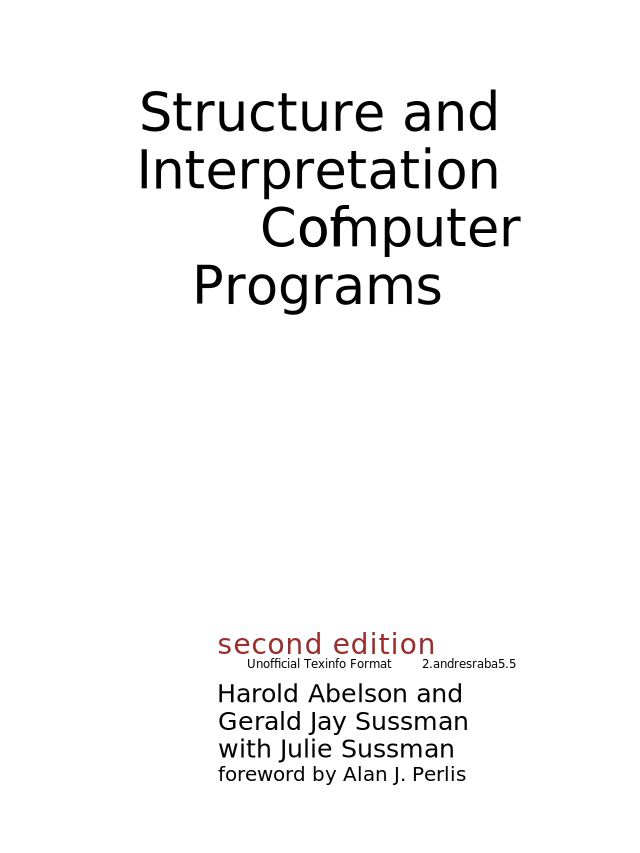
\includepdf[scale=0.92]{coverpage.pdf}

\pagebreak

\vspace*{\fill}
\thispagestyle{empty}

\begin{small}

\noindent
{\copyright}1996 by The Massachusetts Institute of Technology

\vspace{1.26em}
\noindent
Structure and Interpretation of Computer Programs,\\
second edition

\vspace{1.26em}
\noindent
Harold Abelson and Gerald Jay Sussman\\
with Julie Sussman, foreword by Alan J. Perlis

\vspace{1.6em}
\noindent

\includegraphics[width=25mm]{fig/icons/by-nc-sa.pdf}

\vspace{0.4em}
\noindent
This work is licensed under a Creative Commons\\ 
Attribution-NonCommercial-ShareAlike 3.0 Unported License\\
(\href{http://creativecommons.org/licenses/by-nc-sa/3.0/}{\acronym{CC BY-NC-SA} 3.0}).
Based on a work at \href{http://mitpress.mit.edu/sicp/}{mitpress.mit.edu}.

\vspace{1.26em}
\noindent
The \acronym{MIT} Press\\
Cambridge, Massachusetts\\ 
London, England

\vspace{1.26em}
\noindent
McGraw-Hill Book Company\\
New York, St. Louis, San Francisco,\\ 
Montreal, Toronto

\vspace{1.26em}
\noindent
Unofficial Texinfo Format \href{http://sicpebook.wordpress.com}{2.andresraba5.2} (February 10, 2014),\\ 
based on \href{http://www.neilvandyke.org/sicp-texi/}{2.neilvandyke4} (January 10, 2007).

\vspace{1.26em}
\noindent
日本語: by \href{http://d.hatena.ne.jp/minghai/}{minghai} based on 2.andresraba5.2 (March 31, 2014).

\end{small}

\pagebreak

\tableofcontents

\small  % Added by minghai. (Japanese fonts looks too big.)

%=======================================================================================================

\label{UTF}
\chapter*{Unofficial Texinfo Format}
\addcontentsline{toc}{chapter}{Unofficial Texinfo Format}

This is the second edition \acronym{SICP} book, from Unofficial Texinfo
Format.

これは\acronym{SICP}の第二版非公式Texinfo版です。

You are probably reading it in an Info hypertext browser, such as the Info
mode of Emacs.  You might alternatively be reading it {\TeX}-formatted on your
screen or printer, though that would be silly.  And, if printed, expensive.

あなたは恐らくこれをEmacsのInfoモードの様なハイパーテキストブラウザで読んで
いることでしょう。他にも{\TeX}で組版した物を画面や印刷して読んでいるかもしれませんが
それはバカバカしい上に高くつきます。

The freely-distributed official \acronym{HTML}-and-\acronym{GIF} format was
first converted personally to Unofficial Texinfo Format (\acronym{UTF})
version 1 by Lytha Ayth during a long Emacs lovefest weekend in April, 2001.

公式に無料で公開された\acronym{HTML}-and-\acronym{GIF}版を
Lytha Aythが最初に私的に、2001年4月の長いEmacs Lovefest Weekendの間に
非公式Texinfo版(\acronym{UTF})バージョン1へと変換しました。

The \acronym{UTF} is easier to search than the \acronym{HTML} format.  It is
also much more accessible to people running on modest computers, such as
donated '386-based PCs.  A 386 can, in theory, run Linux, Emacs, and a Scheme
interpreter simultaneously, but most 386s probably can't also run both Netscape
and the necessary X Window System without prematurely introducing budding young
underfunded hackers to the concept of \newterm{thrashing}.  UTF can also fit
uncompressed on a 1.44\acronym{MB} floppy diskette, which may come in handy for
installing UTF on PCs that do not have Internet or LAN access.

\acronym{UTF}はHTML版よりも検索がより簡単です。また寄付された古い386の様な
質素な計算機上で行う人々にとってよりアクセスが容易です。386は理論的にはLinux、Emacs、
Schemeインタプリタを同時に実行できます。しかし多くの386は恐らくNetscapeと必要なX Window
Systemを事前に芽の出かけた資金不足の若いハッカーに\newterm{thrashing}(スラッシング)の
概念を教えることなしに動かすことはできないでしょう。UTFはまた圧縮無しでも1.44\acronym{MB}
のフロッピーディスケットに収まります。これはインターネットやLANへの接続環境の無いPC
にインストールする場合に役立つでしょう。

The Texinfo conversion has been a straight transliteration, to the extent
possible.  Like the {\TeX}-to-\acronym{HTML} conversion, this was not without
some introduction of breakage.  In the case of Unofficial Texinfo Format,
figures have suffered an amateurish resurrection of the lost art of
\acronym{ASCII}.  Also, it's quite possible that some errors of ambiguity
were introduced during the conversion of some of the copious superscripts (`\^{}')
and subscripts (`\_').  Divining \emph{which} has been left as an exercise to
the reader. But at least we don't put our brave astronauts at risk by encoding
the \emph{greater-than-or-equal} symbol as \code{<u>\&gt;</u>}.

Texinfoへの変換は可能な範囲での直接的な翻字でした。{\TeX}-to-\acronym{HTML}変換の様に
ある程度の破れが含まれること無しにはできませんでした。非公式TexInfo形式においては
図が「失なわれた技術」であるアスキーアートによる下手糞な"復活"を被りました。また
多量の上付き文字と下付き文字のいくつかの変換の間に不明瞭さによる変換の
失敗が含まれてしまった可能性が大いにあります。読者への課題として残されたと予測します。
しかし、最低でも\emph{``以上''}の記号を\texttt{<u>\&gt;</u>}と符号化することで
我等の勇敢な宇宙飛行士を危険に晒すようなことはしませんでした。

If you modify \texttt{sicp.texi} to correct errors or improve the
\acronym{ASCII} art, then update the \code{@set utfversion {utfversion}}
line to reflect your delta.  For example, if you started with Lytha's version
\code{1}, and your name is Bob, then you could name your successive versions
\code{1.bob1}, \code{1.bob2},  \dots , \code{1.bob\textit{n}}.  Also update
\code{utfversiondate}.  If you want to distribute your version on the Web, then
embedding the string ``sicp.texi'' somewhere in the file or Web page will make
it easier for people to find with Web search engines.


もしあなたが\texttt{sicp.texi}を変更しエラーを訂正したり、アスキーアートを向上させたなら
\code{@set utfversion {utfversion}}の行を更新し、あなたの修正を反映して下さい。
例えば、もしあなたがLythaのバージョン\code{1}で開始し、あなたの名前がBobなら、改訂版は
\code{1.bob1}, \code{1.bob2}, \dots , \code{1.bob\textit{n}}です。また\code{utfversiondate}も更新
して下さい。もしあなたが自分の改訂版をWeb上で配布したいのなら文字列``sicp.texi''を
ファイルやWebページのどこかに埋め込んでおけば人々にとってWeb検索エンジンから
探すことが簡単になるでしょう。

It is believed that the Unofficial Texinfo Format is in keeping with the
spirit of the graciously freely-distributed \acronym{HTML} version.  But you
never know when someone's armada of lawyers might need something to do, and get
their shorts all in a knot over some benign little thing, so think twice before
you use your full name or distribute Info, \acronym{DVI}, PostScript, or
\acronym{PDF} formats that might embed your account or machine name.

非公式Texinfo形式は寛大にも自由の下に配布された\acronym{HTML}版の魂を引き継いで
いると信じられています。しかし、いつ誰かの法律家の大艦隊が良心に基づく小さな事に対して非常に腹を立て
何かを行わなければならなくなるかもしれません。ですのであなたのフルネームを
使ったり、あなたのアカウントやマシン名を含むInfo, \acronym{DVI}, PostScript, \acronym{PDF}形式
を配布する前に良く良く考えて下さい。

\noindent
\textit{Peath, Lytha Ayth}

\vspace{1.0em}
\noindent
\textbf{Addendum:} See also the \acronym{SICP} video lectures by Abelson and Sussman:\\
at \href{http://groups.csail.mit.edu/mac/classes/6.001/abelson-sussman-lectures/}{\acronym{MIT CSAIL}} or 
\href{http://ocw.mit.edu/courses/electrical-engineering-and-computer-science/6-001-structure-and-interpretation-of-computer-programs-spring-2005/video-lectures/}{\acronym{MIT OCW}}.

\textbf{付録:}AbelsonとSussmanによる\acronym{SICP}のビデオレクチャーもご覧下さい。\\
\href{http://groups.csail.mit.edu/mac/classes/6.001/abelson-sussman-lectures/}{\acronym{MIT CSAIL}}
\href{http://ocw.mit.edu/courses/electrical-engineering-and-computer-science/6-001-structure-and-interpretation-of-computer-programs-spring-2005/video-lectures/}{\acronym{MIT OCW}}.


\vspace{0.5em}
\noindent 
\textbf{Second Addendum:} Above is the original introduction to the \acronym{UTF} 
from 2001. Ten years later, \acronym{UTF} has been transformed: mathematical 
symbols and formulas are properly typeset, and figures drawn in 
vector graphics. The original text formulas and \acronym{ASCII} art figures 
are still there in the Texinfo source, but will display only when compiled 
to Info output. At the dawn of e-book readers and tablets, reading a 
\acronym{PDF} on screen is officially not silly anymore. Enjoy!

\noindent
\textbf{付録2:} 上記は2001年の元の\acronym{UTF}の紹介です。
10年後、\acronym{UTF}は一変しました。数学上の記号と式は適切に組版され、図は
ベクターグラフィックにより描かれています。元のテキスト形式とアスキーアートの図
は今でもTexinfoのソースに残っていますが、Info形式でコンパイルした場合のみ
表示されます。電子書籍リーダーとタブレットの夜明けに画面上で\acronym{PDF}を
読むことは正式に、最早バカバカしいことでは無くなりました。楽しんで下さい!

\vspace{0.5em}
\noindent
\textit{A.R, May, 2011}

%============================================================================================================

\label{Dedication}
\chapter*{Dedication}
\addcontentsline{toc}{chapter}{Dedication}

\lettrine{T}{his book is dedicated}, in respect and admiration, to the spirit that lives in
the computer.

この本を、尊敬と賛美を込めて、コンピュータの中に住む妖精に捧げます。

\begin{quote}
``I think that it's extraordinarily important that we in computer science keep
fun in computing.  When it started out, it was an awful lot of fun. Of course,
the paying customers got shafted every now and then, and after a while we began
to take their complaints seriously.  We began to feel as if we really were
responsible for the successful, error-free perfect use of these machines. 
I don't think we are.  I think we're responsible for stretching them, setting
them off in new directions, and keeping fun in the house.  I hope the field of
computer science never loses its sense of fun.  Above all, I hope we don't
become missionaries.  Don't feel as if you're Bible salesmen.   The world has
too many of those already.  What you know about computing other people will
learn. Don't feel as if the key to successful computing is only in your hands.
What's in your hands, I think and hope, is intelligence: the ability to see the
machine as more than when you were first led up to it, that you can make it
more.''

``コンピュータサイエンスに関わる私達にとってコンピュータを使用することを
楽しむことはとても大事だと私は考えます。コンピュータサイエンスが始まった時、それは
とても多くの楽しみに溢れていました。
ご存知のとおり、お金を払うお客様達は時折酷く騙されました。そして暫くして私達は
彼らの不満を真面目に受け取り始めてしまいました。
私達は考え始めてしまったのです。成功裏に、障害の無い完全なコンピュータの使用法に
ついて私達に責任があるのではないかと。
私はそうは思いません。
私は、私達がコンピュータサイエンスを伸展し、新しい方向に向かわせ、
そして仲間達と共に楽しむことに責任があると考えます。
私はコンピュータサイエンスの現場が楽しむことの感覚を失わないことを望みます。
さらに、我々が伝道師になることは望みません。
自分が聖書のセールスマンだとは思わないで下さい。
世界には既にそのような人が溢れています。
あなたが他の人々が学ぶコンピュータ利用法について何を知っているでしょう。
コンピュータ利用に成功する鍵があなたの手の中にのみあるとは決っして思わないで
下さい。
 私が思うに、そして期待することは、あなたの手の中にあるものは知性です。
それはあなたが初めて計算機に出会った時よりもより多くのことを知ることができる
能力であり、それはより多くのことを生むことができるのです。''

\noindent
---Alan J. Perlis (April 1, 1922 -- February 7, 1990)
\end{quote}

%===========================================================================================================

\label{Foreword}
\chapter*{Foreword}
\addcontentsline{toc}{chapter}{Foreword}

\vspace{-0.6em}

Educators, generals, dieticians, psychologists, and parents program.  Armies,
students, and some societies are programmed.  An assault on large problems
employs a succession of programs, most of which spring into existence en route.
These programs are rife with issues that appear to be particular to the problem
at hand.  To appreciate programming as an intellectual activity in its own
right you must turn to computer programming; you must read and write computer
programs---many of them.  It doesn't matter much what the programs are about or
what applications they serve.  What does matter is how well they perform and
how smoothly they fit with other programs in the creation of still greater
programs.  The programmer must seek both perfection of part and adequacy of
collection.  In this book the use of ``program'' is focused on the creation,
execution, and study of programs written in a dialect of Lisp for execution on
a digital computer.  Using Lisp we restrict or limit not what we may program,
but only the notation for our program descriptions.

教育者、将軍、栄養士、精神分析医、そして両親はプログラムします。軍隊、学生、そして
いくつかの社会はプログラムされます。大きな問題に対する解決は一連のプログラムを
利用します。それらのほとんどは途中でひょっこり表れます。これらのプログラムは手近な
問題に特化されて現れる成果に溢れています。プログラミングを独立した知的な活動として
理解するためにはあなたはコンピュータプログラミングに向かわねばなりません。
コンピュータプログラムを読み、書かねばなりません。それも数多くです。そのプログラムが何に
ついてであるか、またはどのような適用を担うのかは多くは関係ありません。
重要なことはそれらがどのように実行され、どれだけ滑らかに他のプログラムに対してより
大きなプログラムの作成のために適合するのかです。プログラマは部分の完全性と集合の
妥当性の両方を追求せねばなりません。この本では``プログラム''の使用はデジタル計算機上にて
実行されるためのLispの方言で書かれたプログラムの創造、実行、それに学習に焦点を当てて
います。Lispの使用はプログラム記述の表記法のみを制約、制限し、私達が何をプログラムするか
については影響を与えません。

Our traffic with the subject matter of this book involves us with three foci of
phenomena: the human mind, collections of computer programs, and the computer.
Every computer program is a model, hatched in the mind, of a real or mental
process.  These processes, arising from human experience and thought, are huge
in number, intricate in detail, and at any time only partially understood.
They are modeled to our permanent satisfaction rarely by our computer programs.
Thus even though our programs are carefully handcrafted discrete collections of
symbols, mosaics of interlocking functions, they continually evolve: we change
them as our perception of the model deepens, enlarges, generalizes until the
model ultimately attains a metastable place within still another model with
which we struggle.  The source of the exhilaration associated with computer
programming is the continual unfolding within the mind and on the computer of
mechanisms expressed as programs and the explosion of perception they generate.
If art interprets our dreams, the computer executes them in the guise of
programs!

この本の主題は3つの事象に焦点を当てます。人の心、コンピュータプログラムの集合、そして
コンピュータです。全てのコンピュータプログラムは人の心の中で生まれる現実の、または
精神的な過程のモデルです。これらの過程は人の経験と思考から浮かび上がり、数はとても
多く、詳細は入り組んで、いつでも部分的にしか理解されません。それらはコンピュータ
プログラムにより稀にしか永遠の充足としてモデル化されることはありません。従って、
例え私達のプログラムが注意深く手作りされた別個の記号の集合だとしても、連動する機能の
寄せ集めだとしても、それらは絶えず発展します。私達のモデルの知覚がより深まるにつれ、
増えるにつれ、一般化されるにつれ、モデルが究極的に準安定な位置に逹っするまで変更を
行い、その中には依然として私達が格闘するモデルが存在します。コンピュータプログラミングに
関連する歓喜の源はプログラムとして表現された仕組みの心の中とコンピュータ上で絶え間無く
続く発展であり、それにより生まれる知力の爆発です。もし技巧が私達の夢を解釈するならば、
コンピュータはプログラムとして現わされるそれらを実行するのです!


For all its power, the computer is a harsh taskmaster.  Its programs must be
correct, and what we wish to say must be said accurately in every detail.  As
in every other symbolic activity, we become convinced of program truth through
argument.  Lisp itself can be assigned a semantics (another model, by the way),
and if a program's function can be specified, say, in the predicate calculus,
the proof methods of logic can be used to make an acceptable correctness
argument.  Unfortunately, as programs get large and complicated, as they almost
always do, the adequacy, consistency, and correctness of the specifications
themselves become open to doubt, so that complete formal arguments of
correctness seldom accompany large programs.  Since large programs grow from
small ones, it is crucial that we develop an arsenal of standard program
structures of whose correctness we have become sure---we call them idioms---and
learn to combine them into larger structures using organizational techniques of
proven value.  These techniques are treated at length in this book, and
understanding them is essential to participation in the Promethean enterprise
called programming.  More than anything else, the uncovering and mastery of
powerful organizational techniques accelerates our ability to create large,
significant programs.  Conversely, since writing large programs is very taxing,
we are stimulated to invent new methods of reducing the mass of function and
detail to be fitted into large programs.

その力全てに対して、コンピュータは厳しい親方です。そのプログラムは正しくなければ
なりません。私達が伝えたいと望む事柄は委細全て正確に伝えられねばなりません。
全ての他の象徴的な活動と同じく、私達は議論を通してプログラムの真理を確信するように
なります。Lispそれ自身に意味論を割り当てることも可能です。(ところでこれはまた別の
モデルです)。そしてもしプログラムの機能を指定できるのなら、例えば述語論理においてなら、
論理の証明方法が容認可能な正確性の議論に使用できます。残念なことにプログラムが巨大で
複雑になるにつれ、そしてほとんど常にそうなるのですが、仕様の妥当性、一貫性、正確さそれら
自身が疑わしくなります。そのため完全に形式化された正確さの議論は巨大なプログラムには
伴いません。巨大プログラムは小さな物から成長するため正確さに確信を持てる標準的な
プログラム構造の武器庫を開発することは重要です。私達はこれをidiom(イディオム)と呼びます。
そしてそれらを組み合わせて価値が検証された構成技術を用いてより大きな構造にすることを
学びます。これらの技術はこの本の中で長々と扱われます。そしてそれらを理解することは
プログラミングと呼ばれるプロメテウスの進取性(Promethean enterprise)に参加するのに
絶対に必要なことです。他の何事でもなく、強力な構成技術を暴き熟達することは巨大で
重要なプログラムを作成する能力を加速します。反対に、巨大なプログラムを書くことはとても
苦労が多いため、私達は多大な機能や詳細を巨大プログラムに合うように減らす新しい手法
を開発することを促されています。

Unlike programs, computers must obey the laws of physics.  If they wish to
perform rapidly---a few nanoseconds per state change---they must transmit
electrons only small distances (at most \(1 {1\over2}\) feet). The heat generated by
the huge number of devices so concentrated in space has to be removed.  An
exquisite engineering art has been developed balancing between multiplicity of
function and density of devices.  In any event, hardware always operates at a
level more primitive than that at which we care to program.  The processes that
transform our Lisp programs to ``machine'' programs are themselves abstract
models which we program.  Their study and creation give a great deal of insight
into the organizational programs associated with programming arbitrary models.
Of course the computer itself can be so modeled.  Think of it: the behavior of
the smallest physical switching element is modeled by quantum mechanics
described by differential equations whose detailed behavior is captured by
numerical approximations represented in computer programs executing on
computers composed of \dots !

プログラムとは異なり、コンピュータは物理法則に従わなければなりません。もし
それらを迅速に動かしたいのならば---状態変更当たり2、3ナノ秒で---コンピュータは
電子を極小の距離で転送せねばなりません(高々\(1{1\over2}\) フィート)。
巨大な数の端子により生じる熱は空間に集中しますがこれは取り除かねばなりません。
精緻な工学の技芸が機能の多重度と端子の密度の間のバランスを取るために開発されました。
任意のイベントにおいて、ハードウェアは常に私達がプログラムを行うのに気にするよりも
よりプリミティブなレベルで動作します。私達のLispプログラムを``機械の''プログラムに
変換する処理はそれ自体が私達がプログラムする抽象モデルです。それらの学習と作成は
とても多くの見識をプログラミングの自由裁量なモデルに関連する組織的なプログラムに
対して与えます。もちろんコンピュータそれ自身もそのようにモデル化可能です。そのことを
考えてみましょう。最小の物理スイッチング要素の振舞は量子力学でモデル化され、微分
方程式により記述され、その詳細な振舞は近似値の数値演算により獲得され、それは
コンピュータプログラムにより表現され、それはコンピュータ上で実行され、それは
組み立てられ\dots !

It is not merely a matter of tactical convenience to separately identify the
three foci.  Even though, as they say, it's all in the head, this logical
separation induces an acceleration of symbolic traffic between these foci whose
richness, vitality, and potential is exceeded in human experience only by the
evolution of life itself.  At best, relationships between the foci are
metastable.  The computers are never large enough or fast enough.  Each
breakthrough in hardware technology leads to more massive programming
enterprises, new organizational principles, and an enrichment of abstract
models.  Every reader should ask himself periodically ``Toward what end, toward
what end?''---but do not ask it too often lest you pass up the fun of
programming for the constipation of bittersweet philosophy.

3つの焦点を別々に判別することは戦術上の利便性の問題でしかありません。
例え良く言われるように全てが頭の中にあるとしても、この論理的分割はこれらの焦点の
間の記号的通信量の加速を引き起します。焦点の豊かさ、活力、潜在力は人間の
経験の中で人生自体の発展により増加します。最良時には焦点の間の関係は準安定に
なります。コンピュータは絶対に十分に大きく、速くはなりません。ハードウェア技術の
全ての飛躍的進歩がより大規模なプログラミング計画、新しい組織化原理、抽象モデルの
向上へと導きます。読者の全員が自身に対し繰り返し``どの終点に向かって? どの終端に向かって?''と
問わねばなりません。しかしあまり問い過ぎてもいけません。ほろ苦い哲学の便秘のために
プログラミングの楽しさを逸っしてしまいます。

Among the programs we write, some (but never enough) perform a precise
mathematical function such as sorting or finding the maximum of a sequence of
numbers, determining primality, or finding the square root.  We call such
programs algorithms, and a great deal is known of their optimal behavior,
particularly with respect to the two important parameters of execution time and
data storage requirements.  A programmer should acquire good algorithms and
idioms.  Even though some programs resist precise specifications, it is the
responsibility of the programmer to estimate, and always to attempt to improve,
their performance.

私達が書くプログラムの間で、いくつか(しかし絶対に十分ではない)は厳格な数学上の
関数、例えばソートや数列の最大値を見つける、素数性判定、平方根を求める等が実行されます。
私達はそのようなプログラムをアルゴリズムと呼びます。多数の物がそれらの最適な振舞を、
特に2つの重要なパラメタである実行時間とデータストレージの必要量に関して知られています。
プログラマは良いアルゴリズムとイディオムを獲得しなければなりません。
例えいくつかのプログラムが厳格な仕様に反しても、それらのパフォーマンスに関して
見積り、常に改善に努めることはプログラマの責務です。

Lisp is a survivor, having been in use for about a quarter of a century.  Among
the active programming languages only Fortran has had a longer life.  Both
languages have supported the programming needs of important areas of
application, Fortran for scientific and engineering computation and Lisp for
artificial intelligence.  These two areas continue to be important, and their
programmers are so devoted to these two languages that Lisp and Fortran may
well continue in active use for at least another quarter-century.

Lispは``生存者''であり約四半世紀の間利用されてきました。活発なプログラミング言語の中で
FortranのみがLispより長い人生を経ています。LispとFortranはどちらもアプリケーションの重要な領域の
プログラミング上の必要性に対処してきました。すなわちFortranは科学計算や工学計算に対して、
Lispは人工知能に対してです。これらの2つの領域は重要で有り続けており、そこに携わっている
プログラマ達はこれら2つの言語に専念しているため、LispとFortranは少なくとももう四半期は
活発に使われ続けることでしょう。

Lisp changes.  The Scheme dialect used in this text has evolved from the
original Lisp and differs from the latter in several important ways, including
static scoping for variable binding and permitting functions to yield functions
as values.  In its semantic structure Scheme is as closely akin to Algol 60 as
to early Lisps.  Algol 60, never to be an active language again, lives on in
the genes of Scheme and Pascal.  It would be difficult to find two languages
that are the communicating coin of two more different cultures than those
gathered around these two languages.  Pascal is for building
pyramids---imposing, breathtaking, static structures built by armies pushing
heavy blocks into place.  Lisp is for building organisms---imposing,
breathtaking, dynamic structures built by squads fitting fluctuating myriads of
simpler organisms into place.  The organizing principles used are the same in
both cases, except for one extraordinarily important difference: The
discretionary exportable functionality entrusted to the individual Lisp
programmer is more than an order of magnitude greater than that to be found
within Pascal enterprises.  Lisp programs inflate libraries with functions
whose utility transcends the application that produced them.  The list, Lisp's
native data structure, is largely responsible for such growth of utility.  The
simple structure and natural applicability of lists are reflected in functions
that are amazingly nonidiosyncratic.  In Pascal the plethora of declarable data
structures induces a specialization within functions that inhibits and
penalizes casual cooperation.  It is better to have 100 functions operate on
one data structure than to have 10 functions operate on 10 data structures.  As
a result the pyramid must stand unchanged for a millennium; the organism must
evolve or perish.

Lispは変化します。このテキストで使用されるScheme方言はオリジナルのLispから発展し
いくつかの重要な手法に関して異なっています。違いには変数束縛に対する静的スコーピングや
関数の値として関数の生成を許可している点等が含まれます。その意味構造においてSchemeは
初期のLispと同等にAlgol 60に近い物です。Algol 60は再び現役となることはないでしょうが、
SchemeとPascalの遺伝子に受け継がれています。
これらの2つの言語の周りに集った言語よりも、もう2つの異なる文化の流通貨幣としての
2つの言語を見つけることのほうが難しいでしょう。
Pascalはピラミッドを建築するための物です---印象的で、息を飲むような、軍隊が重い
ブロックを所定の位置に押すことで建築された静的な構造物です。Lispは有機体を構築
するための物です---印象的で、息を飲むような、小分隊が不安定で無数のより単純な有機体を
所定の位置に嵌め込むことで構築された動的な構築物です。使用された体系化の原則は
両者の場合で同じです。ただし並外れて重要な違いが1つあります。個々のLispプログラマに
委ねられた任意のエクスポート可能な機能の数はPascalの進取性の中に見つかるそれらよりも桁違いに多いのです。
Lispプログラムは機能のライブラリを膨らませます。その機能の実用性はそれらを生成した
アプリケーションを越えます。Lisp生来のデータ構造であるリストがそのような実用性の成長の
大きな原因です。簡単な構造と自然なリストの適用可能性が驚くべき程に非特異的に機能に
反映されています。Pascalでは宣言可能なデータ構造の過剰さがカジュアルな連携を抑止し、ペナルティを科す
機能の中に特殊化することを促しています。1つのデータ構造の上で操作する100の機能を持つほうが
10のデータ構造の上で操作する10の機能を持つよりも優れています。結果としてピラミッドは1000年の間
変わらぬままでいるに違いありませんが、有機体は発展できなければ滅んでしまうのです。

To illustrate this difference, compare the treatment of material and exercises
within this book with that in any first-course text using Pascal.  Do not labor
under the illusion that this is a text digestible at \acronym{MIT} only,
peculiar to the breed found there.  It is precisely what a serious book on
programming Lisp must be, no matter who the student is or where it is used.

この違いを説明するためにはこの本の中にある教材と課題の扱いを任意の初級課程の
Pascalを用いるテキストのそれと比べてみて下さい。\acronym{MIT}だけが消費できる、
そこで見つかる血統書付きの良馬のためのものという幻想の下で苦悩しないで下さい。学生が
誰であるかとかどこで利用されるかが問題ではありません。まさに、
Lispプログラミングに対して真剣な本はどんな物であるべきかが問題です。

Note that this is a text about programming, unlike most Lisp books, which are
used as a preparation for work in artificial intelligence.  After all, the
critical programming concerns of software engineering and artificial
intelligence tend to coalesce as the systems under investigation become larger.
This explains why there is such growing interest in Lisp outside of artificial
intelligence.

これはプログラミングに関するテキストであることに注意して下さい。人工知能の仕事のための
予習に使われる他の多くのLispの本とは違います。結局、ソフトウェア工学と人工知能の重大な
プログラミングの課題は研究がより大きくなるにつれシステムとして融合する傾向にあります。
このことがなぜそのようなLispへの興味が人工知能の外側で大きくなっているのかを説明します。

As one would expect from its goals, artificial intelligence research generates
many significant programming problems.  In other programming cultures this
spate of problems spawns new languages.  Indeed, in any very large programming
task a useful organizing principle is to control and isolate traffic within the
task modules via the invention of language.  These languages tend to become
less primitive as one approaches the boundaries of the system where we humans
interact most often.  As a result, such systems contain complex
language-processing functions replicated many times.  Lisp has such a simple
syntax and semantics that parsing can be treated as an elementary task.  Thus
parsing technology plays almost no role in Lisp programs, and the construction
of language processors is rarely an impediment to the rate of growth and change
of large Lisp systems.  Finally, it is this very simplicity of syntax and
semantics that is responsible for the burden and freedom borne by all Lisp
programmers.  No Lisp program of any size beyond a few lines can be written
without being saturated with discretionary functions.  Invent and fit; have
fits and reinvent!  We toast the Lisp programmer who pens his thoughts within
nests of parentheses.

誰かがそのゴールから予測したように、人工知能研究は多くの明確なプログラミング上の問題を
生成しました。他のプログラミング文化ではこの相次ぐ問題は新しい言語を生みます。実際に
どんなとても大きなプログラミングタスクにおいても効果的な体系化原理はタスクモジュール内の
情報量を言語の発明を通してコントロールし、分離することです。これらの言語は
私達、人間が最も良く操作を行うシステムの境界へと辿り着くに従いプリミティブではなくなっていく
傾向にあります。結果として、そのようなシステムは何度も複製された複雑な言語処理機能を含みます。
Lispはとてもシンプルな文法と意味論を持ち、パースが初歩的なタスクとして扱えます。
従ってパースの技術はLispプログラムにおいてはほとんどルール無用の役割を演じます。そして
言語処理機の構築は巨大なLispシステムの変化と成長の程度に対しほとんど障害になりません。
最後に、全てのLispプログラマにより負われている義務と自由に対して責任を持つものこそが
このとても単純な文法と意味論です。数行のサイズを越えるLispプログラムなら自由裁量による
関数で満たすことなく書くことはできません。開発し、合わせる。合わせて、また開発する!
括弧の入れ子の中に自身の考えを記述するLispプログラマに乾杯。

\vspace{0.5em}
\noindent
Alan J. Perlis\\
New Haven, Connecticut

%=========================================================================================================

\label{Preface}
\chapter*{Preface to the Second Edition}
\addcontentsline{toc}{chapter}{Preface to the Second Edition}

\begin{quote}
Is it possible that software is not like anything else, that it is meant to be
discarded: that the whole point is to always see it as a soap bubble?

ソフトウェアが他の何物にも似ていないと言うことはできるでしょうか。それが捨てられる
べき物だと。つまり、常にシャボン玉だと見なすことだと。

---Alan J. Perlis
\end{quote}

\vspace{0.7em}

\noindent
The material in this book has been the basis of \acronym{MIT}'s entry-level
computer science subject since 1980.  We had been teaching this material for
four years when the first edition was published, and twelve more years have
elapsed until the appearance of this second edition.  We are pleased that our
work has been widely adopted and incorporated into other texts.  We have seen
our students take the ideas and programs in this book and build them in as the
core of new computer systems and languages.  In literal realization of an
ancient Talmudic pun, our students have become our builders.  We are lucky to
have such capable students and such accomplished builders.

この本の中の教材は1980年から\acronym{MIT}の入門者レベルの計算機科学の科目の中心となる物です。
私達はこの教材を4年間、最初の版が出版された時点で教えてきました。そしてこの第二版が出現する
までにさらに12年が経過しました。私達の成果が広く受け入れられ、他のテキストに取り込まれている
ことを喜ばしく思っています。私達の生徒がこの本の考えとプログラムを学び新しい計算機システムと
言語の核としてそれらを組み込んでいるのを見てきました。古代のタルムードの多義語の文字認識では、
私達の生徒が開発者になってくれました。そのような能力有る学生と熟練した開発者を得たことは
とても幸運なことでした。

In preparing this edition, we have incorporated hundreds of clarifications
suggested by our own teaching experience and the comments of colleagues at
\acronym{MIT} and elsewhere.  We have redesigned most of the major programming
systems in the book, including the generic-arithmetic system, the interpreters,
the register-machine simulator, and the compiler; and we have rewritten all the
program examples to ensure that any Scheme implementation conforming to the
\acronym{IEEE} Scheme standard (\link{IEEE 1990}) will be able to run the
code.

この版を準備するにあたって、私達自身の教育上の経験と\acronym{MIT}や他の同僚達からの
コメントにより提案された幾百もの説明を統合しました。この本の中の主なプログラミングシステムの
多くを包括的数値演算システム、インタプリタ、レジスタマシンシミュレータ、コンパイラを含めて再設計しました。
そして全てのプログラム例を、任意の\acronym{IEEE} Scheme標準(\link{IEEE 1990})に従うScheme実装が
そられのコードを実行できることを確実にするために、書き直しました。

This edition emphasizes several new themes.  The most important of these is the
central role played by different approaches to dealing with time in
computational models: objects with state, concurrent programming, functional
programming, lazy evaluation, and nondeterministic programming.  We have
included new sections on concurrency and nondeterminism, and we have tried to
integrate this theme throughout the book.

この版はいくつかの新しいテーマを重視しています。これらの内、最も重要なものは
計算モデル内での時間を取り扱うための異なる取り組みにより演じられる中心的な役割です。
状態を伴うオブジェクト、並行プログラミング、関数型プログラミング、遅延評価、そして
非決定性プログラミングです。私達は並行性と非決定性に関わる新しい節を含め、そして
このテーマをこの本を通してまとめることを試みました。

The first edition of the book closely followed the syllabus of our
\acronym{MIT} one-semester subject.  With all the new material in the second
edition, it will not be possible to cover everything in a single semester, so
the instructor will have to pick and choose.  In our own teaching, we sometimes
skip the section on logic programming (\link{Section 4.4}), we have students use
the register-machine simulator but we do not cover its implementation (\link{Section 5.2}), 
and we give only a cursory overview of the compiler (\link{Section 5.5}).  
Even so, this is still an intense course.  Some instructors may
wish to cover only the first three or four chapters, leaving the other material
for subsequent courses.

この本の第一版は\acronym{MIT}の一学期の科目の講義概要を密接に追っていました。
第二版の全ての新しい教材により、一学期で全てをカバーすることは不可能となりました。
そのためインストラクタは選択をしなければなりません。私達自身の教育現場では、
時々論理プログラミング(\link{Section 4.4})を飛ばします。学生にはレジスタマシンの
シミュレータを使用させるのでその実装(\link{Section 5.2})はカバーしません。
そしてコンパイラ(\link{Section 5.5})は概観のみを大雑把に教えています。それでもこれは
依然として強烈な授業です。何人かのインストラクタは最初の3章から4章のみをカバーし、
他の教材を続きの授業に残したいと願うでしょう。

The World-Wide-Web site \href{http://mitpress.mit.edu/sicp}{http://mitpress.mit.edu/sicp} provides
support for users of this book.  This includes programs from the book, sample
programming assignments, supplementary materials, and downloadable
implementations of the Scheme dialect of Lisp.

World-Wide-Webサイト \href{http://mitpress.mit.edu/sicp}{http://mitpress.mit.edu/sicp} はこの本のユーザへのサポートを提供します。
これにはこの本のプログラム、プログラミング課題のサンプル、補助教材、ダウンロード可能なLispの
Scheme方言の実装が含まれます。

%============================================================================================================
\label{Preface 1e}
\chapter*{Preface to the First Edition}
\addcontentsline{toc}{chapter}{Preface to the First Edition}

% \vspace{-0.6em}
\begin{quote}
A computer is like a violin.  You can imagine a novice trying first a
phonograph and then a violin.  The latter, he says, sounds terrible.  That is
the argument we have heard from our humanists and most of our computer
scientists.  Computer programs are good, they say, for particular purposes, but
they aren't flexible.  Neither is a violin, or a typewriter, until you learn
how to use it.

コンピュータはヴァイオリンのような物です。初心者が最初に蓄音機、そして次に
ヴァイオリンを試すことを想像して下さい。彼は後者の音は酷いと言います。
これが人間主義者と多くの計算機科学者から聞こえてくる議論です。
計算機のプログラムは特定の目的には良い物だ、しかし柔軟性が無いと彼らは言います。
ヴァイオリンやタイプライタだって同じです。あなたがその使い方を学ぶまでは。

---Marvin Minsky, ``Why Programming Is a Good Medium for Expressing
Poorly-Understood and Sloppily-Formulated Ideas''
\end{quote}

\vspace{0.8em}

\noindent
``The Structure and Interpretation of Computer Programs'' is the entry-level
subject in computer science at the Massachusetts Institute of Technology.  It
is required of all students at \acronym{MIT} who major in electrical
engineering or in computer science, as one-fourth of the ``common core
curriculum,'' which also includes two subjects on circuits and linear systems
and a subject on the design of digital systems.  We have been involved in the
development of this subject since 1978, and we have taught this material in its
present form since the fall of 1980 to between 600 and 700 students each year.
Most of these students have had little or no prior formal training in
computation, although many have played with computers a bit and a few have had
extensive programming or hardware-design experience.

``The Structure and Interpretation of Computer Programs''(SICP, 計算機プログラムの構造と解釈)は
マサチューセッツ工科大学(MIT)での入門者レベルの
計算機科学の科目です。\acronym{MIT}にて電気工学、または計算機工学を専攻する全ての
学生が``共通コアカリキュラム''の4つの内の1つとして履修しなければなりません。
共通コアカリキュラムは回路と線形システムについて2つの科目とデジタルシステムの
設計についての科目を含みます。私達はこの科目の開発を1978年から行なってきました。
そしてこの教材を現行様式として1980年の秋から、600名から700名の学生に毎年、教えて
きました。これらの学生の多くは少し、または全くの事前の公式な計算機利用についての
トレーニングを受けてはいませんでした。ただし、多くは事前に計算機で少々遊んだ経験が
有り、ほんの少数は広範囲のプログラミングの経験やハードウェア設計の経験がありました。

Our design of this introductory computer-science subject reflects two major
concerns.  First, we want to establish the idea that a computer language is not
just a way of getting a computer to perform operations but rather that it is a
novel formal medium for expressing ideas about methodology.  Thus, programs
must be written for people to read, and only incidentally for machines to
execute.  Second, we believe that the essential material to be addressed by a
subject at this level is not the syntax of particular programming-language
constructs, nor clever algorithms for computing particular functions
efficiently, nor even the mathematical analysis of algorithms and the
foundations of computing, but rather the techniques used to control the
intellectual complexity of large software systems.

私達のこの計算機科学の入門科目の設計は2つの主な関心事を反映しています。1つは、
コンピュータ言語はコンピュータに命令を実行させるための単なる方法等ではなく、
新しい種類の方法論に関する考えを表現するための公式なメディアであるという考えを
証明することです。従ってプログラムは人々が読むために書かれねばならず、そして
ただ偶然に機械にとって実行する物でなければなりません。2つ目は、このレベルの
科目により扱われる本質的な教材とは、特定のプログラミング言語が構築する構文ではなく、
また特定の関数を効率的に演算するための賢いアルゴリズムでもなく、増してアルゴリズムと
演算基盤の数理解析でないという信念です。そうではなく、大きなソフトウェアシステムの
知的な複雑性をコントロールするために用いる技術でなければなりません。

Our goal is that students who complete this subject should have a good feel for
the elements of style and the aesthetics of programming.  They should have
command of the major techniques for controlling complexity in a large
system. They should be capable of reading a 50-page-long program, if it is
written in an exemplary style. They should know what not to read, and what they
need not understand at any moment.  They should feel secure about modifying a
program, retaining the spirit and style of the original author.

私達の目標は、この教科を完了した学生がプログラミングの美学とスタイルの原理に対して
必ず良い感触を得ることです。学生達が大きなシステムの複雑性をコントロールするための
主な技術の能力を得られなければなりません。学生達が50ページの長さのプログラムを、
それが模範的なスタイルで書かれているのならば、読めるようにならなければなりません。
学生達がプログラムの変更を行う時に、元の作者の魂とスタイルを維持しながら安心できな
ければなりません。

These skills are by no means unique to computer programming.  The techniques we
teach and draw upon are common to all of engineering design.  We control
complexity by building abstractions that hide details when appropriate.  We
control complexity by establishing conventional interfaces that enable us to
construct systems by combining standard, well-understood pieces in a ``mix and
match'' way.  We control complexity by establishing new languages for
describing a design, each of which emphasizes particular aspects of the design
and deemphasizes others.

これらのスキルは決してコンピュータプログラミングに対して独自なことではありません。
私達が教え、利用する技術は全ての工学設計に対して共通な物です。私達は
適切な場合に、詳細を隠す抽象概念を構築することにより複雑性をコントロールします。
標準的な、良く理解された部品を``mix and match''(様々な物をうまく組み合わせる方法)の方法により
組み合わせることにより、システムを構築することを可能にする慣習的なインターフェイスを
確立することで、複雑性をコントロールします。私達は設計を記述するための新しい言語を
確立することで複雑性をコントロールします。そして各言語は設計の特定の側面を重要視し、
他の側面の重要性を緩和します。

Underlying our approach to this subject is our conviction that ``computer
science'' is not a science and that its significance has little to do with
computers.  The computer revolution is a revolution in the way we think and in
the way we express what we think.  The essence of this change is the emergence
of what might best be called \newterm{procedural epistemology}---the study of
the structure of knowledge from an imperative point of view, as opposed to the
more declarative point of view taken by classical mathematical subjects.
Mathematics provides a framework for dealing precisely with notions of ``what
is.''  Computation provides a framework for dealing precisely with notions of
``how to.''

私達のこの教科に対する取り組み方の根底を成す物は、``計算機科学''は科学ではなく、
その意義は計算機とは関係が無いという信念です。計算機革命とは私達の考え方と
私達の考えの表現方法における革命です。この変化の本質を恐らく最もうまく言い表わす
のは\newterm{procedural epistemology}(手続的認識論)---古典的な数学上の主題により
取られるより宣言的な視点に対立する、命令型の視点からの知識構造の研究---の出現でしょう。
数学は``何であるか''の概念を正確に扱うためのフレームワークを提供します。計算機の使用は
``行い方''の概念を正確に扱うためのフレームワークを提供します。

In teaching our material we use a dialect of the programming language Lisp.  We
never formally teach the language, because we don't have to.  We just use it,
and students pick it up in a few days.  This is one great advantage of
Lisp-like languages: They have very few ways of forming compound expressions,
and almost no syntactic structure.  All of the formal properties can be covered
in an hour, like the rules of chess.  After a short time we forget about
syntactic details of the language (because there are none) and get on with the
real issues---figuring out what we want to compute, how we will decompose
problems into manageable parts, and how we will work on the parts.  Another
advantage of Lisp is that it supports (but does not enforce) more of the
large-scale strategies for modular decomposition of programs than any other
language we know.  We can make procedural and data abstractions, we can use
higher-order functions to capture common patterns of usage, we can model local
state using assignment and data mutation, we can link parts of a program with
streams and delayed evaluation, and we can easily implement embedded languages.
All of this is embedded in an interactive environment with excellent support
for incremental program design, construction, testing, and debugging.  We thank
all the generations of Lisp wizards, starting with John McCarthy, who have
fashioned a fine tool of unprecedented power and elegance.

私達の教材を教えるにあたって、プログラミング言語Lispの一方言を使用します。
私達は正式にこの言語を教えることはしません。する必要がないからです。
ただそれを使用し、そして学生は2、3日で習熟してしまいます。これはLispの様な
言語の1つの利点です。これらの言語は複合式を形成する方法があまり多くありません。
そしてほとんど構文構造が存在しません。形式的な特性の全ては一時間もあれば
カバーできます。まるでチェスのルールの様なものです。少しの時間の後にはこの
言語の構文上の詳細を忘れてしまいます。(ほとんど存在しないからです)。そして
本当の問題---私達が演算したい物を把握すること、どのように問題を扱いやすい
部分へと分解するか、そしてどのようにその部品上で働くかについて取り掛かります。
Lispのもう1つの利点は私達が知っている他のどの言語よりもプログラムを分解した
モジュラに対するより多くの大規模な戦略をサポートする(しかし強制はしない)ことです。
手続化とデータ抽象化を行い、公開関数を用いて処理の共通なパターンを獲得し、代入と
データの変更を用いて局所状態のモデル化を行い、プログラムの部品をストリームと遅延評価に
結び付け、簡単に組込言語を実装することができます。これら全てがインタラクティブ(相互作用)な
環境にインクリメンタル(漸増的な)プログラム設計、構築、テスト、デバッグのための
優れたサポートと共に組込まれています。私達は前例の無い力と洗練さを供えた素晴しいツールを
創り出したJohn McCarthyを始めとする全ての世代のLisp wizard(ウィザード、魔法使い、
最上級のプログラマの賞賛を込めた呼び名)に感謝します。

Scheme, the dialect of Lisp that we use, is an attempt to bring together the
power and elegance of Lisp and Algol.  From Lisp we take the metalinguistic
power that derives from the simple syntax, the uniform representation of
programs as data objects, and the garbage-collected heap-allocated data.  From
Algol we take lexical scoping and block structure, which are gifts from the
pioneers of programming-language design who were on the Algol committee.  We
wish to cite John Reynolds and Peter Landin for their insights into the
relationship of Church's \(\lambda\)-calculus to the structure of programming
languages.  We also recognize our debt to the mathematicians who scouted out
this territory decades before computers appeared on the scene.  These pioneers
include Alonzo Church, Barkley Rosser, Stephen Kleene, and Haskell Curry.

私達が用いるLispの方言、SchemeはLispとAlgolの力と洗練を一緒にもたらそうとしました。
Lispからは単純な構文から導き出されるメタ言語の力、データオブジェクトとしてのプログラムの
単一の表現、ガベージコレクションを持つヒープ上に取得されるデータを得ました。
AlgolからはAlgol委員会に在籍したプログラム設計の開拓者からの贈り物である
レキシカルスコープとブロック構造を得ました。私達はJohn ReynoldsとPeter Landinの
Church(チャーチ)の\(lambda\)-calculus(ラムダ計算)のプログラミング言語の構造に
対する関係についての彼等の洞察に対して言及したいと願います。
またコンピュータがこの世界に現れる何十年も前にこの領域を偵察された数学者達に対する
恩義も忘れておりません。これらの開拓者にはAlonzo Church, Barkley Rosser, Stephen Kleene,
Haskell Curry等が含まれております。

%============================================================================================================
\label{Acknowledgements}
\chapter*{Acknowledgements}
\addcontentsline{toc}{chapter}{Acknowledgements}

We would like to thank the many people who have helped us develop this book and
this curriculum.

この本とこのカリキュラムの開発を手助けして下さった多くの人々に感謝致します。

Our subject is a clear intellectual descendant of ``6.231,'' a wonderful
subject on programming linguistics and the \( \lambda \)-calculus taught at
\acronym{MIT} in the late 1960s by Jack Wozencraft and Arthur Evans, Jr.

私達の教科は明らかに1960年代の終わりに\acronym{MIT}にてJack Wozencraftと
Arthur Evans, Jr.により教えられたプログラミング言語学と\( \lambda \)演算上の
素晴しい科目、``6.231''の知的末裔です。

We owe a great debt to Robert Fano, who reorganized \acronym{MIT}'s
introductory curriculum in electrical engineering and computer science to
emphasize the principles of engineering design.  He led us in starting out on
this enterprise and wrote the first set of subject notes from which this book
evolved.

私達はRobert Fanoに大きな借りがあります。彼は\acronym{MIT}の電気工学と計算機科学の
導入部のカリキュラムを再編成し、工学設計の原理を重視しました。彼はこの進取性への
着手に導き、またこの本への発展の元となる最初の教科ノートのまとめを記述しました。

Much of the style and aesthetics of programming that we try to teach were
developed in conjunction with Guy Lewis Steele Jr., who collaborated with
Gerald Jay Sussman in the initial development of the Scheme language.  In
addition, David Turner, Peter Henderson, Dan Friedman, David Wise, and Will
Clinger have taught us many of the techniques of the functional programming
community that appear in this book.

私達が教えようとするプログラミングのスタイルと美学の多くは
Guy Lewis Steele Jr.の協力の下に開発されました。彼は初期のSchemeの開発において
Gerald Jay Sussmanと協力を行いました。加えてDavid Turner, Peter Henderson, 
Dan Friedman, David Wise, Will Clingerが私達にこの本の中に現れる関数型プログラミングの
テクニックの多くを教えてくれました。

Joel Moses taught us about structuring large systems.  His experience with the
Macsyma system for symbolic computation provided the insight that one should
avoid complexities of control and concentrate on organizing the data to reflect
the real structure of the world being modeled.

Joel Mosesは私達に巨大システムの構造化について教えてくれました。彼の記号演算のための
Macsymaシステムにおける経験が、人は制御の複雑性を回避し、データの体系化に集中して
モデル化されていく世界の真の構造を反映するべきだという見識を与えてくれました。

Marvin Minsky and Seymour Papert formed many of our attitudes about programming
and its place in our intellectual lives.  To them we owe the understanding that
computation provides a means of expression for exploring ideas that would
otherwise be too complex to deal with precisely.  They emphasize that a
student's ability to write and modify programs provides a powerful medium in
which exploring becomes a natural activity.

Marvin MinskyとSeymour Papertは私達のプログラミングに関する態度の多くと、
私達の知的な生活内にそれの場所を形作りました。彼等に対して、考えを探求するための
式の意味を演算が与えることについての理解に借りがあります。そうでなければ、
正確に取り扱うためには複雑過ぎることになってしまいます。彼らは学生のプログラムを
書き、変更する能力が、その中で探求が自然な活動になる強力なメディアを提供すると
強調します。

We also strongly agree with Alan Perlis that programming is lots of fun and we
had better be careful to support the joy of programming.  Part of this joy
derives from observing great masters at work.  We are fortunate to have been
apprentice programmers at the feet of Bill Gosper and Richard Greenblatt.

私達はまたプログラミングは大いに楽しく、このプログラミングの楽しみをサポートする
ために十分に注意しなければならない点についてAlan Perlisに強く同意します。
この楽しみの一部は作業中の偉大な職人達を観察することから得られます。
私達は幸運なことに、Bill GosperとRichard Greenblattの下で見習いプログラマで
いることができました。

It is difficult to identify all the people who have contributed to the
development of our curriculum.  We thank all the lecturers, recitation
instructors, and tutors who have worked with us over the past fifteen years and
put in many extra hours on our subject, especially Bill Siebert, Albert Meyer,
Joe Stoy, Randy Davis, Louis Braida, Eric Grimson, Rod Brooks, Lynn Stein and
Peter Szolovits.  We would like to specially acknowledge the outstanding
teaching contributions of Franklyn Turbak, now at Wellesley; his work in
undergraduate instruction set a standard that we can all aspire to.  We are
grateful to Jerry Saltzer and Jim Miller for helping us grapple with the
mysteries of concurrency, and to Peter Szolovits and David McAllester for their
contributions to the exposition of nondeterministic evaluation in \link{Chapter
4}.

私達のカリキュラムの開発に貢献して下さった全ての人々を特定することは難しいことです。
私達は過去15年私達と共に働き、多くの時間を私達の教科に費してくれた全ての講師、
口答の指導者、チューターに、
特に、Bill Siebert, Albert Meyer,
Joe Stoy, Randy Davis, Louis Braida, Eric Grimson, Rod Brooks, Lynn Stein and
Peter Szolovitsに感謝します。
私達は特に卓越した教育上の貢献として現在はウェルズリーのFranklyn Turbakに感謝します。
彼の学部生向け指導要項は私達皆が目指す基準を打ち立てました。
Jerry SaltzerとJim Millerには私達が並行性のミステリーに取り組むのを手助けして下さった
ことに感謝します。そしてPeter SzolovitsとDavid McAllesterには\link{Chapter
4}における非決定性評価の説明に対する貢献に感謝します。

Many people have put in significant effort presenting this material at other
universities.  Some of the people we have worked closely with are Jacob
Katzenelson at the Technion, Hardy Mayer at the University of California at
Irvine, Joe Stoy at Oxford, Elisha Sacks at Purdue, and Jan Komorowski at the
Norwegian University of Science and Technology.  We are exceptionally proud of
our colleagues who have received major teaching awards for their adaptations of
this subject at other universities, including Kenneth Yip at Yale, Brian Harvey
at the University of California at Berkeley, and Dan Huttenlocher at Cornell.

多くの人々は他大学でこの資料を紹介するのに大きな努力を費してくださいました。
私達が親密に働いたそれらの人々の幾人かはイスラエル工科大学のJacob Katzenelson、
カリフォルニア大学アーバイン校のHardy Mayer、オックスフォード大学のJoe Stoy、
パデュー大学のElisha Sacks、ノルウェー技術科学大学のJan Komorowskiです。
私達は他大学においてこの科目を受け入れることで主要な教育の賞を受けた同僚達を
非常に誇りに思います。この中にはイェール大学のKenneth Yip、カリフォルニア大学
バークリー校のBrian Harvey、コーネル大学のDan Huttenlocherを含みます。

Al Moy\'e arranged for us to teach this material to engineers at
Hewlett-Packard, and for the production of videotapes of these lectures.  We
would like to thank the talented instructors---in particular Jim Miller, Bill
Siebert, and Mike Eisenberg---who have designed continuing education courses
incorporating these tapes and taught them at universities and industry all over
the world.

Al Moy\'eは私たちのためにこの教材をHPの技術者達に教える手筈とこのレクチャーのビデオ
テープの製品化を準備してくれました。私たちはまた才能あるインストラクター達にも
感謝致します。具体的にはJim Miller, Bill Siebert, Mike Eisenbergです。彼等は
これらのテープを組み込んで生涯教育のコースを設計し、世界中の大学と業界にて
教育を行いました。

Many educators in other countries have put in significant work translating the
first edition.  Michel Briand, Pierre Chamard, and Andr\'e Pic produced a
French edition; Susanne Daniels-Herold produced a German edition; and Fumio
Motoyoshi produced a Japanese edition.  We do not know who produced the Chinese
edition, but we consider it an honor to have been selected as the subject of an
``unauthorized'' translation.

他国の多くの教育者が多大な時間を第一版の翻訳に費して下さいました。
Michel Briand, Pierre Chamard, and Andr\'e Picはフランス語版をプロデュースして下さいました。
Susanne Daniels-Heroldはドイツ語版をプロデュースして下さいました。
元吉文男は日本語版をプロデュースして下さいました。私たちはどなたが中国語版を
プロデュースして下さったのか知りません。しかし``未許可''の翻訳の題材として
選ばれたことを光栄に思います。

It is hard to enumerate all the people who have made technical contributions to
the development of the Scheme systems we use for instructional purposes.  In
addition to Guy Steele, principal wizards have included Chris Hanson, Joe
Bowbeer, Jim Miller, Guillermo Rozas, and Stephen Adams.  Others who have put
in significant time are Richard Stallman, Alan Bawden, Kent Pitman, Jon Taft,
Neil Mayle, John Lamping, Gwyn Osnos, Tracy Larrabee, George Carrette, Soma
Chaudhuri, Bill Chiarchiaro, Steven Kirsch, Leigh Klotz, Wayne Noss, Todd Cass,
Patrick O'Donnell, Kevin Theobald, Daniel Weise, Kenneth Sinclair, Anthony
Courtemanche, Henry M. Wu, Andrew Berlin, and Ruth Shyu.

私たちが教育の目的のために使用するSchemeシステムの開発に技術的な貢献をされた全ての
人々を列挙することは難しいことです。Guy Steeleに加えて、主要なウィザードの中にはChris Hanson, Joe
Bowbeer, Jim Miller, Guillermo Rozas, and Stephen Adamsが含まれます。
多大な時間を費して下さった他の人々はRichard Stallman, Alan Bawden, Kent Pitman, Jon Taft,
Neil Mayle, John Lamping, Gwyn Osnos, Tracy Larrabee, George Carrette, Soma
Chaudhuri, Bill Chiarchiaro, Steven Kirsch, Leigh Klotz, Wayne Noss, Todd Cass,
Patrick O'Donnell, Kevin Theobald, Daniel Weise, Kenneth Sinclair, Anthony
Courtemanche, Henry M. Wu, Andrew Berlin, それにRuth Shyuです。

Beyond the \acronym{MIT} implementation, we would like to thank the many people
who worked on the \acronym{IEEE} Scheme standard, including William Clinger and
Jonathan Rees, who edited the \( \rm R^4RS \), and Chris Haynes, David Bartley,
Chris Hanson, and Jim Miller, who prepared the \acronym{IEEE} standard.

\acronym{MIT}の実装を越えて、私たちは\acronym{IEEE}のScheme標準仕様について
働いた多くの人々に感謝したいと思います。\( \rm R^4RS \)を編集したWilliam Clingerと
Jonathan Rees、\acronym{IEEE}標準を準備したChris Haynes, David Bartley,
Chris Hanson, Jim Millerを含みます。

Dan Friedman has been a long-time leader of the Scheme community.  The
community's broader work goes beyond issues of language design to encompass
significant educational innovations, such as the high-school curriculum based
on EdScheme by Schemer's Inc., and the wonderful books by Mike Eisenberg and by
Brian Harvey and Matthew Wright.

Dan Friedmanは長い間Schemeコミュニティのリーダーでした。コミュニティの広範な仕事は
言語設計の問題を越えて、Schemer's Inc.によるEdSchemeを基にした高校生向けカリキュラムや
Mike EisenbergやBrian HarveyとMatthew Wrightによる素晴しい本のような、特筆すべき
教育上のイノベーションを含むまでに至りました。

We appreciate the work of those who contributed to making this a real book,
especially Terry Ehling, Larry Cohen, and Paul Bethge at the \acronym{MIT}
Press.  Ella Mazel found the wonderful cover image.  For the second edition we
are particularly grateful to Bernard and Ella Mazel for help with the book
design, and to David Jones, {\TeX} wizard extraordinaire.  We also are indebted
to those readers who made penetrating comments on the new draft: Jacob
Katzenelson, Hardy Mayer, Jim Miller, and especially Brian Harvey, who did unto
this book as Julie did unto his book \textit{Simply Scheme}.

私たちはこの本を現実にすることに貢献して下さった人々の働きに感謝致します。
特に\acronym{MIT}出版のTerry Ehling, Larry Cohen, Paul Bethgeです。
Ella Mazelは素晴しいカバーの絵を見つけてくれました。第二版に対しては特にこの本の
デザインを助けてくれたBernardとEllaのMazel夫妻、非凡な{\TeX}ウィザードである
David Jonesに感謝致します。私たちはまた新しいドラフトに対し洞察力のあるコメントを
して下さった読者の方々、Jacob Katzenelson, Hardy Mayer, Jim Miller, そして特に
Brian Harveyに対して、Julieが彼の本\textit{Simply Scheme}に行ったように、この本に
行ってくれたことを感謝致します。

Finally, we would like to acknowledge the support of the organizations that
have encouraged this work over the years, including suppport from
Hewlett-Packard, made possible by Ira Goldstein and Joel Birnbaum, and support
from \acronym{DARPA}, made possible by Bob Kahn.

最後に、何年にも渡ったこの仕事を励まして下さった組織のサポートに感謝したいと思います。
Hewlett-Packardからのサポートを可能にして下さったIra GoldsteinとJoel Birnbaum、
それに\acronym{DARPA}からのサポートを可能にして下さったBob Kahnを含みます。

%============================================================================================================

\pagenumbering{arabic}

\mainmatter

\label{Chapter 1}
\chapter{手続を用いた抽象化の構築}

\begin{quote}
The acts of the mind, wherein it exerts its power over simple ideas, are
chiefly these three: 1. Combining several simple ideas into one compound one,
and thus all complex ideas are made.  2. The second is bringing two ideas,
whether simple or complex, together, and setting them by one another so as to
take a view of them at once, without uniting them into one, by which it gets
all its ideas of relations.  3.  The third is separating them from all other
ideas that accompany them in their real existence: this is called abstraction,
and thus all its general ideas are made.

心がその中で、その力を単純な考えの上に発揮する``心の働き''は、主としてこれら3つです。1. いくつかの
簡単な考えを1つの複合物に組み合わせます。全ての複雑な考えはこのようにして作られます。
2. 2つの考えをそれが簡単であるか複雑であるかに係らず一緒にもたらし、お互いに
合わせることでそれらを統合することは無しに、全ての関係性の考えを得ることで、一度に
それらを見渡します。3. 考えをそれらの実在に付随する全ての他の考えから分離します。
これは抽象化と呼ばれ、このようにして全てのその一般的な考えは作られます。

---John Locke, \emph{An Essay Concerning Human Understanding} (1690)
\end{quote}

\vspace{1.0em}

\noindent
We are about to study the idea of a \newterm{computational process}.
Computational processes are abstract beings that inhabit computers.  As they
evolve, processes manipulate other abstract things called \newterm{data}.  The
evolution of a process is directed by a pattern of rules called a
\newterm{program}.  People create programs to direct processes.  In effect, we
conjure the spirits of the computer with our spells.

私達は\newterm{computational process}(演算プロセス)について学びます。演算プロセスとは抽象的な存在で
コンピュータ
の中に複数が住んでいます。それらが進化するとプロセスは\newterm{data}(データ)と呼ばれる
また別の抽象的な物を扱います。プロセスの進化は\newterm{program}(プログラム)と呼ばれるルールの
パターン(型、類型)により命じられます。人はプログラムを作成してプロセスに命ずるのです。
つまり私達はコンピュータの精霊に私達の呪文で魔法をかけるのです。

A computational process is indeed much like a sorcerer's idea of a spirit.  It
cannot be seen or touched.  It is not composed of matter at all.  However, it
is very real.  It can perform intellectual work.  It can answer questions.  It
can affect the world by disbursing money at a bank or by controlling a robot
arm in a factory.  The programs we use to conjure processes are like a
sorcerer's spells.  They are carefully composed from symbolic expressions in
arcane and esoteric \newterm{programming languages} that prescribe the tasks we
want our processes to perform.

演算プロセスは本当に魔法使いの精霊の考えに似ています。それは見たり触れたりは
できません。物理的な物では構成されていません。しかしとてもリアルな存在です。
知的な仕事を行います。質問にも答えます。銀行でお金を払ったり、工場でロボットの
腕をコントロールすることで世界に影響を与えることも可能です。私達が利用する
プロセスに魔法をかけるプログラムとは魔法使いの呪文のような物です。難解な秘伝の
\newterm{programming languages}(プログラミング言語)の中で記号的表現にて慎重に組み立てられプロセスに
実行してほしいタスク(仕事、任務)を指示します。

A computational process, in a correctly working computer, executes programs
precisely and accurately.  Thus, like the sorcerer's apprentice, novice
programmers must learn to understand and to anticipate the consequences of
their conjuring.  Even small errors (usually called \newterm{bugs} or
\newterm{glitches}) in programs can have complex and unanticipated
consequences.

演算プロセスは、正しく動くコンピュータでは、精密に正しくプログラムを実行します。
従って魔法使いの見習いのように、初心者のプログラマは魔法の結果について理解し、
予測することを学ばねばなりません。例えプログラムの小さなエラー
(通常は\newterm{bugs}(バグ)、または\newterm{glitches}(グリッチ、誤作動)と呼ばれます)でも
複雑で予測不可能な結果をもたらす場合もあるのです。

Fortunately, learning to program is considerably less dangerous than learning
sorcery, because the spirits we deal with are conveniently contained in a
secure way.  Real-world programming, however, requires care, expertise, and
wisdom.  A small bug in a computer-aided design program, for example, can lead
to the catastrophic collapse of an airplane or a dam or the self-destruction of
an industrial robot.

幸運なことに、プログラムを学ぶことは魔法を学ぶことより少しも危険ではありません。
私達が相手にする精霊は都合良く安全な方法で封じ込まれています。
しかし、実際の世界でのプログラミングには注意力、専門知識、堅実さを必要とします。
例えばCAD(計算機による設計支援)プログラムの小さなバグが飛行機や
ダムの最悪な崩壊に繋ったり、工業ロボットの自己破壊を起こしたりします。

Master software engineers have the ability to organize programs so that they
can be reasonably sure that the resulting processes will perform the tasks
intended.  They can visualize the behavior of their systems in advance.  They
know how to structure programs so that unanticipated problems do not lead to
catastrophic consequences, and when problems do arise, they can \newterm{debug}
their programs.  Well-designed computational systems, like well-designed
automobiles or nuclear reactors, are designed in a modular manner, so that the
parts can be constructed, replaced, and debugged separately.

ソフトウェアエンジニアのマスター達は最終的にプロセスが望まれたタスクを実行する
ことに自信を持てるだけの技能を、プログラムの構築に対して持っています。
彼らは前もってシステムの行いを図で説明することができます。予測不可能な問題が
最悪な結果をもたらさぬようプログラムをどのように構造化を行うのか知っています。
そして問題が発生した時にはプログラムの \newterm{debug}(デバッグ、バグ取り)を行えます。
良い設計のコンピュータシステムは、良い設計の自動車や原子炉のように
モジュール方式で設計されており、パーツは個別に組み立て、置き換え、デバッグが
可能です。

\subsubsection*{Lispプログラミング}

We need an appropriate language for describing processes, and we will use for
this purpose the programming language Lisp.  Just as our everyday thoughts are
usually expressed in our natural language (such as English, French, or
Japanese), and descriptions of quantitative phenomena are expressed with
mathematical notations, our procedural thoughts will be expressed in Lisp.
Lisp was invented in the late 1950s as a formalism for reasoning about the use
of certain kinds of logical expressions, called \newterm{recursion equations},
as a model for computation.  The language was conceived by John McCarthy and is
based on his paper ``Recursive Functions of Symbolic Expressions and Their
Computation by Machine'' (\link{McCarthy 1960}).

私達はプロセスを記述するのに適切な言語を必要とします。この目的に対しプログラミング
言語Lispを利用します。私達の日々の考えが通常、自然言語(例えば英語やフランス語、
日本語)で表されるように、定量的な現象が数学の記号で表されるように、手続的な
思考はLispで表現されます。Lispは1950年代後半に\newterm{recursion equations}(再帰方程式)
と呼ばれるある種の論理表現に関する推論のための形式化として開発されました。
この言語はJohn McCarthyにより着想され、彼の論文``記号式の再帰方程式とそれらの機械による演算''
(\link{McCarthy 1960})を基にしています。

Despite its inception as a mathematical formalism, Lisp is a practical
programming language.  A Lisp \newterm{interpreter} is a machine that carries
out processes described in the Lisp language.  The first Lisp interpreter was
implemented by McCarthy with the help of colleagues and students in the
Artificial Intelligence Group of the \acronym{MIT} Research Laboratory of
Electronics and in the \acronym{MIT} Computation Center.\footnote{The
\textit{Lisp 1 Programmer's Manual} appeared in 1960, and the \textit{Lisp 1.5
Programmer's Manual} (\link{McCarthy et al. 1965}) was published in 1962.  The early history
of Lisp is described in \link{McCarthy 1978}.}  Lisp, whose name is an acronym for
LISt Processing, was designed to provide symbol-manipulating capabilities for
attacking programming problems such as the symbolic differentiation and
integration of algebraic expressions.  It included for this purpose new data
objects known as atoms and lists, which most strikingly set it apart from all
other languages of the period.

数学上の形式主義としての始まりにも関わらず、Lispは実用的なプログラミング言語
です。Lisp\newterm{interpreter}(インタプリタ、逐次翻訳処理器)はLisp言語にて記述されたプロセスを実行する
機械です。最初のLispインタプリタはMcCarthyと\acronym{MIT}研究所の人工知能部門の
同僚、学生による手助けにて実装されました。\footnote{
\textit{Lisp 1 Programmer's Manual}は1960年に初出し、
\textit{Lisp 1.5 Programmer's Manual} (\link{McCarthy et al. 1965})は1962年に出版
されました。Lispの初期の歴史は\link{McCarthy 1978}にて説明されています。}
Lispはその名前をLIst Processing(リスト処理)の頭文字から取っており、
記号微分や代数式の積分の様なプログラミング上の問題に着手するための
記号操作能力を提供するために設計されました。この目的のためにアトムとリストとして
知られる新しいデータオブジェクトを含みます。これはその時代の他の全ての言語から
著しく際立たせる物でした。

Lisp was not the product of a concerted design effort.  Instead, it evolved
informally in an experimental manner in response to users' needs and to
pragmatic implementation considerations.  Lisp's informal evolution has
continued through the years, and the community of Lisp users has traditionally
resisted attempts to promulgate any ``official'' definition of the language.
This evolution, together with the flexibility and elegance of the initial
conception, has enabled Lisp, which is the second oldest language in widespread
use today (only Fortran is older), to continually adapt to encompass the most
modern ideas about program design.  Thus, Lisp is by now a family of dialects,
which, while sharing most of the original features, may differ from one another
in significant ways.  The dialect of Lisp used in this book is called
Scheme.\footnote{The two dialects in which most major Lisp programs of the
1970s were written are MacLisp (\link{Moon 1978}; \link{Pitman 1983}), developed at the
\acronym{MIT} Project \acronym{MAC}, and Interlisp (\link{Teitelman 1974}), developed
at Bolt Beranek and Newman Inc. and the Xerox Palo Alto Research Center.
Portable Standard Lisp (\link{Hearn 1969}; \link{Griss 1981}) was a Lisp dialect designed to
be easily portable between different machines.  MacLisp spawned a number of
subdialects, such as Franz Lisp, which was developed at the University of
California at Berkeley, and Zetalisp (\link{Moon and Weinreb 1981}), which was based on a
special-purpose processor designed at the \acronym{MIT} Artificial Intelligence
Laboratory to run Lisp very efficiently.  The Lisp dialect used in this book,
called Scheme (\link{Steele and Sussman 1975}), was invented in 1975 by Guy Lewis Steele Jr. and
Gerald Jay Sussman of the \acronym{MIT} Artificial Intelligence Laboratory and
later reimplemented for instructional use at \acronym{MIT}.  Scheme became an
\acronym{IEEE} standard in 1990 (\link{IEEE 1990}).  The Common Lisp dialect
(\link{Steele 1982}, \link{Steele 1990}) was developed by the Lisp community to combine
features from the earlier Lisp dialects to make an industrial standard for
Lisp.  Common Lisp became an \acronym{ANSI} standard in 1994 (\link{ANSI 1994}).}

Lispは計画的な設計の取り組みから生まれた製品ではありませんでした。そうではなく、
非公式に試験的なやり方で、ユーザの要求と実利的な実装上の考慮への対応として発展しました。
Lispの非公式な進化は何年も続き、Lispユーザのコミュニティは伝統的に言語の``公式な''
どんな定義の公表に対しても抵抗しました。この進化は初期構想の柔軟性と洗練さと共に、今日
世界中で広く使用される言語で2番目に古い(Fortranのみがより古い)言語として、Lispに継続的に
最新のプログラム設計についての考えを受け入れることを可能にしてきました。
従ってLispは今では複数の方言の系統が存在し、それらはオリジナルの機能の多くを共有しながらも、
お互いに大きな違いを持ちます。この本で使用されるLispの方言はSchemeと呼ばれます。\footnote{
1970年代に最もメジャーなLispプログラムの記述に用いられた2つの方言は\acronym{MIT}のプロジェクト
\acronym{MAC}で開発されたMacLisp (\link{Moon 1978}; \link{Pitman 1983})と
Bolt Beranek and Newman Inc.とXerox Palo Alto研究センターににて開発された
Interlisp (\link{Teitelman 1974})でした。Portable Standard Lisp (\link{Hearn 1969}; \link{Griss 1981})
は簡単に、異なるマシンの間で移植可能にするよう設計されたLisp方言です。MacLispは
カリフォルニア大学バークレー校により開発されたFranz Lispや\acronym{MIT}人工知能研究所が
Lispをとても効率良く実行するために設計した特定目的プロセッサ(処理機)をベースにした
Zetalisp (\link{Moon and Weinreb 1981})といったいくつかの下位方言を生みました。
この本で使用するLisp方言はSheme (\link{Steele and Sussman 1975})と呼ばれ、1975年に
\acronym{MIT}人工知能研究所のGuy Lewis Steele Jr.とGerald Jay Sussmanにより開発され、
後に\acronym{MIT}にて教育目的のために再実装されました。
Common Lisp (\link{Steele 1982}, \link{Steele 1990})はLispコミュニティにより初期のLisp方言の
機能を集約し、Lispの業界標準を作成するために開発されました。Common Lispは1994年に
\acronym{ANSI}標準(\link{ANSI 1994})になりました。
}

Because of its experimental character and its emphasis on symbol manipulation,
Lisp was at first very inefficient for numerical computations, at least in
comparison with Fortran.  Over the years, however, Lisp compilers have been
developed that translate programs into machine code that can perform numerical
computations reasonably efficiently.  And for special applications, Lisp has
been used with great effectiveness.\footnote{One such special application was a
breakthrough computation of scientific importance---an integration of the
motion of the Solar System that extended previous results by nearly two orders
of magnitude, and demonstrated that the dynamics of the Solar System is
chaotic.  This computation was made possible by new integration algorithms, a
special-purpose compiler, and a special-purpose computer all implemented with
the aid of software tools written in Lisp (\link{Abelson et al. 1992}; \link{Sussman and Wisdom 1992}).}  
Although Lisp has not yet overcome its old reputation as
hopelessly inefficient, Lisp is now used in many applications where efficiency
is not the central concern.  For example, Lisp has become a language of choice
for operating-system shell languages and for extension languages for editors
and computer-aided design systems.

実験的であるという特徴と記号操作の重要性のため、Lispは初期においては数値演算に対し
少くともFortranとの比較にてとても非効率でした。しかし年を追って、プログラムを
機械語に変換し、数値演算を適度に効率良く実行可能なLispコンパイラが開発されました。
特別なアプリケーションに対してはLispは最高の効果を発揮しています。\footnote{
そのような特別なアプリケーションの1つは自然科学上の重大な計算、太陽系の動きの統合
におけるブレイクスルーでした。これは以前の結果より二桁も良く、太陽系の活動が混沌
であることを実演しました。この計算は全てLispで書かれたソフトウェアツールの手助け
により実装された新しい統合アルゴリズム、特定目的のコンパイラ、特定目的の計算機に
より可能となりました。(\link{Abelson et al. 1992}; \link{Sussman and Wisdom 1992})}
Lispは今でもどうしようもなく非効率であるという古い評判を乗り越えられてはいませんが、
Lispは今では多くのアプリケーションにて、効率が問題の中心ではない場合において
利用されています。例えばLispはOSのシェル言語やエディタの拡張言語、CADシステム等に
おいて選択言語となっています。

If Lisp is not a mainstream language, why are we using it as the framework for
our discussion of programming?  Because the language possesses unique features
that make it an excellent medium for studying important programming constructs
and data structures and for relating them to the linguistic features that
support them.  The most significant of these features is the fact that Lisp
descriptions of processes, called \newterm{procedures}, can themselves be
represented and manipulated as Lisp data.  The importance of this is that there
are powerful program-design techniques that rely on the ability to blur the
traditional distinction between ``passive'' data and ``active'' processes.  As
we shall discover, Lisp's flexibility in handling procedures as data makes it
one of the most convenient languages in existence for exploring these
techniques.  The ability to represent procedures as data also makes Lisp an
excellent language for writing programs that must manipulate other programs as
data, such as the interpreters and compilers that support computer languages.
Above and beyond these considerations, programming in Lisp is great fun.

もしLispがメインストリームの言語でなければなぜ私達はプログラミングの議論のための
フレームワークとしてそれを用いるのでしょうか? なぜならこの言語は
重要なプログラミング構成概念とデータ構造を学ぶため、またそれらをサポートする
言語上の機能にそれらを関連付けするために、言語自身を洗練された媒体と成す個有の機能
を持っているためです。
これらの機能で最も著しい物は、Lispによる\newterm{procedures}(プロシジャ、手続)と
呼ばれるプロセスの記述が、それ自身がLispのデータとして表現され、また操作されることが可能
であるという事実です。これの重要性は、伝統的な``受動的な''データと``能動的な''
プロセスとの間の区別をぼかす能力に依存する、強力なプログラム設計のテクニックが存在する
ということです。私達がそれを発見するにつれ、手続をデータとして扱うLispの柔軟性は
Lispをこれらのテクニックを探求するのに、既存で最も便利な言語の1つとします。
手続をデータとして表現する能力はまた、Lispを他のプログラムをデータとして操作しなければ
ならないプログラムを書く目的に対し洗練された言語にします。例えばコンピュータ言語に
対応するインタプリタやコンパイラのようなプログラムです。これらの考慮点に加えて、
Lispによるプログラミングはとても楽しいのです。



\label{Section 1.1}
\section{The Elements of Programming}

A powerful programming language is more than just a means for instructing a
computer to perform tasks.  The language also serves as a framework within
which we organize our ideas about processes.  Thus, when we describe a
language, we should pay particular attention to the means that the language
provides for combining simple ideas to form more complex ideas.  Every powerful
language has three mechanisms for accomplishing this:

強力なプログラミング言語はコンピュータにタスクの実行を指示するだけではありません。
そのような言語は私達がプロセスについての自らの考えを体系化するフレームワークとして
の役目を担います。従って言語を記述する時、簡単なアイデアを組み合わせてより複雑な
アイデアを形成するという手段をその言語が提供することには特に注意を払わねばなりません。
強力な言語全てがこれを達成するために3つのメカニズムを持っています。

\begin{itemize}

\item \textbf{プリミティブな式},
言語に関わる最も単純な要素を表現する

\item \textbf{合成化の手段},
by which compound elements are built from simpler ones, and
これにより、より単純なものより複合要素が構築される

\item \textbf{抽象化の手段},
by which compound elements can be named and manipulated as units.
これにより複合要素は名前を付けて個体として扱える

\end{itemize}

\noindent
In programming, we deal with two kinds of elements: procedures and data. (Later
we will discover that they are really not so distinct.)  Informally, data is
``stuff'' that we want to manipulate, and procedures are descriptions of the
rules for manipulating the data.  Thus, any powerful programming language
should be able to describe primitive data and primitive procedures and should
have methods for combining and abstracting procedures and data.

プログラミングにおいては2つの種類の要素を扱います。手続(procedure)とデータです。
(後でそれらはあまりはっきりとは区別できないことを明かします。)
簡単に説明するとデータは操作対象の``物''で手続はデータの操作のためのルールの
記述です。従って強力なプログラミング言語はどれもプリミティブ(原始的な、最低レベルの、組込の)なデータと
プリミティブな手続を記述可能でなければならず、また手続とデータを
合成化、抽象化する手法を持たなければなりません。

In this chapter we will deal only with simple numerical data so that we can
focus on the rules for building procedures.\footnote{The characterization of
numbers as ``simple data'' is a barefaced bluff.  In fact, the treatment of
numbers is one of the trickiest and most confusing aspects of any programming
language.  Some typical issues involved are these: Some computer systems
distinguish \newterm{integers}, such as 2, from \newterm{real numbers}, such as
2.71.  Is the real number 2.00 different from the integer 2?  Are the
arithmetic operations used for integers the same as the operations used for
real numbers?  Does 6 divided by 2 produce 3, or 3.0?  How large a number can
we represent?  How many decimal places of accuracy can we represent?  Is the
range of integers the same as the range of real numbers?  Above and beyond
these questions, of course, lies a collection of issues concerning roundoff and
truncation errors---the entire science of numerical analysis.  Since our focus
in this book is on large-scale program design rather than on numerical
techniques, we are going to ignore these problems.  The numerical examples in
this chapter will exhibit the usual roundoff behavior that one observes when
using arithmetic operations that preserve a limited number of decimal places of
accuracy in noninteger operations.} In later chapters we will see that these
same rules allow us to build procedures to manipulate compound data as well.

この章では単純な数値データのみを扱うことにより、手続構築のためのルールに
集中します。\footnote{数値を``単純なデータ''と特徴付けるのは公然なウソです。
実際に数値の扱いは任意のプログラミング言語において最も油断ならない、混乱を招く
要素です。いくつかの典型的な問題は次のものです。いくつかのコンピュータシステムは
2のような\newterm{integers}(整数)と2.71のような\newterm{real numbers}(実数)の区別をします。実数2.00は
整数2とは異なるでしょうか? 整数に用いられる算術演算は実数に対する物と同じでしょ
うか? 6を2で割ったら3? それとも3.0? どれだけ大きな数値を表示できますか? 精度は
小数何桁まで正しく表わされますか? 整数の範囲は実数の範囲と同じですか? もちろん
これらの質問の他にも丸めと切り捨てに関する誤差の問題の蓄積といった数値解析の科学全体が
存在します。この本のフォーカスは大規模なプログラム設計であり数値演算向けの
テクニックではないのでこれらの問題は無視することにします。この章の数値演算の
例では非整数演算において精度上正確な桁数に制限を持つ算術演算を用いる場合に
一般的な丸めの方法を示します。}後の章では同じこれらのルールにより複合データも
また構築できることを学びます。



\label{Section 1.1.1}
\subsection{Expressions}

One easy way to get started at programming is to examine some typical
interactions with an interpreter for the Scheme dialect of Lisp.  Imagine that
you are sitting at a computer terminal.  You type an \newterm{expression}, and
the interpreter responds by displaying the result of its \newterm{evaluating}
that expression.

プログラミングを始める1つの簡単な方法はいくつかの典型的な対話を
Lispの方言であるSchemeのインタプリタを用いて試してみることです。コンピュータ
の端末の前に座っていると想像してみてください。あなたが\newterm{expression}(式)を
入力するとインタプリタはその式の\newterm{evaluation}(評価)の結果を表示することで
応答します。

One kind of primitive expression you might type is a number.  (More precisely,
the expression that you type consists of the numerals that represent the number
in base 10.)  If you present Lisp with a number

あなたが入力するプリミティブな式の一種として数値があります。(より正確には
あなたが入力する式は10進数の数値を表す数字から成り立ちます。)
もし数値をLispに与えた場合、

\begin{scheme}
486
\end{scheme}

\noindent
the interpreter will respond by printing \footnote{Throughout this book, when
we wish to emphasize the distinction between the input typed by the user and
the response printed by the interpreter, we will show the latter in slanted
characters.}

インタプリタは以下を表示することで応答します。\footnote{この本を通して、ユーザの入力
とインタプリタが表示した応答を区別したい場合、傾いた文字で表します。}

\begin{scheme}
~\textit{486}~
\end{scheme}

\noindent
Expressions representing numbers may be combined with an expression
representing a primitive procedure (such as \code{+} or \code{*}) to form a
compound expression that represents the application of the procedure to those
numbers.  For example:

数値を表す式はプリミティブな手続を表す式(例えば\code{+} や \code{*})
と接続することで複合式を形成し、それら数値に対し手続を適用することを表現します。
例えば:

\begin{scheme}
(+ 137 349)
~\textit{486}~
\end{scheme}

\begin{scheme}
(- 1000 334)
~\textit{666}~
\end{scheme}

\begin{scheme}
(* 5 99)
~\textit{495}~
\end{scheme}

\begin{scheme}
(/ 10 5)
~\textit{2}~
\end{scheme}

\begin{scheme}
(+ 2.7 10)
~\textit{12.7}~
\end{scheme}

\noindent
Expressions such as these, formed by delimiting a list of expressions within
parentheses in order to denote procedure application, are called
\newterm{combinations}.  The leftmost element in the list is called the
\newterm{operator}, and the other elements are called \newterm{operands}.  The
value of a combination is obtained by applying the procedure specified by the
operator to the \newterm{arguments} that are the values of the operands.

これらのような式は括弧の中の式のリストを区切ることにより形成され手続の適用を示し、
\newterm{combinations}(組み合わせ)と呼ばれます。リストの最も左の要素は\newterm{operator}(オペレータ、演算子)と呼ばれ、
他の要素は\newterm{operand}(オペランド、被演算数)と呼ばれます。組み合わせの値はオペレータにより
与えられた手続をオペランドの値である\newterm{arguments}(引数)に適用することで得られます。

The convention of placing the operator to the left of the operands is known as
\newterm{prefix notation}, and it may be somewhat confusing at first because it
departs significantly from the customary mathematical convention.  Prefix
notation has several advantages, however.  One of them is that it can
accommodate procedures that may take an arbitrary number of arguments, as in
the following examples:

オペレータをオペランドの左に置く決まりは\newterm{prefix notation}(前置表記法)として
知られています。最初の内は数学の決まりから明らかに逸脱するので混乱するかもしれません。
しかし、前置表記法にはいくつかの利点が存在します。その1つは以下の例のように、
任意の数の引数を取る手続に適応できることです。

\begin{scheme}
(+ 21 35 12 7)
~\textit{75}~
\end{scheme}

\begin{scheme}
(* 25 4 12)
~\textit{1200}~
\end{scheme}

\noindent
No ambiguity can arise, because the operator is always the leftmost element and
the entire combination is delimited by the parentheses.

曖昧さが全くありません。オペレータが常に最も左の要素であり、合成全体
は括弧で区切られているためです。

A second advantage of prefix notation is that it extends in a straightforward
way to allow combinations to be \textit{nested}, that is, to have combinations whose
elements are themselves combinations:

前置表記法の2つ目の利点は直接的な方法にて組み合わせを\textit{nested}(ネスト、入れ子)にすることが可能です。
つまり、組み合わせの要素それ自体が組み合わせである場合です。

\begin{scheme}
(+ (* 3 5) (- 10 6))
~\textit{19}~
\end{scheme}

\noindent
There is no limit (in principle) to the depth of such nesting and to the
overall complexity of the expressions that the Lisp interpreter can evaluate.
It is we humans who get confused by still relatively simple expressions such as

原理的にはそのようなネストの深さとLispインタプリタが評価可能な式全体の複雑さには
制限がありません。しかし私達人間は以下のような比較的単純な式でも混乱してしまいます。

\begin{scheme}
(+ (* 3 (+ (* 2 4) (+ 3 5))) (+ (- 10 7) 6))
\end{scheme}

\noindent
which the interpreter would readily evaluate to be 57.  We can help ourselves
by writing such an expression in the form

インタプリタは直ちに57だと評価するでしょう。このような式を次のような形式で
記述することで私達自身を助けることが可能です。

\begin{scheme}
(+ (* 3
      (+ (* 2 4)
         (+ 3 5)))
   (+ (- 10 7)
      6))
\end{scheme}

\noindent
following a formatting convention known as \newterm{pretty-printing}, in which
each long combination is written so that the operands are aligned vertically.
The resulting indentations display clearly the structure of the
expression.\footnote{Lisp systems typically provide features to aid the user in
formatting expressions.  Two especially useful features are one that
automatically indents to the proper pretty-print position whenever a new line
is started and one that highlights the matching left parenthesis whenever a
right parenthesis is typed.}

\newterm{pretty-printing}(プリティプリント、整形)として知られるフォーマットの決まりに個々の
長いオペランドを従わせることで、オペランドが垂直方向で位置合わせされます。
結果的に式の構造が明確にインデント(字下げ)されることになります。\footnote{典型的な
Lispシステムは式を整形しユーザを手助けするための機能を提供します。特に便利な
2つの機能において、1つは新しい行がどこで始まろうとも自動的に正しい整形位置に
インデントします。もう1つは右括弧が入力された時に対応する左括弧がハイライト
されます。}

Even with complex expressions, the interpreter always operates in the same
basic cycle: It reads an expression from the terminal, evaluates the
expression, and prints the result.  This mode of operation is often expressed
by saying that the interpreter runs in a \newterm{read-eval-print loop}.
Observe in particular that it is not necessary to explicitly instruct the
interpreter to print the value of the expression.\footnote{Lisp obeys the
convention that every expression has a value. This convention, together with
the old reputation of Lisp as an inefficient language, is the source of the
quip by Alan Perlis (paraphrasing Oscar Wilde) that ``Lisp programmers know the
value of everything but the cost of nothing.''}

例え複雑な式でもインタプリタは常に同じ基本的なサイクルにて処理を行います。
式を端末から読み、その式を評価し、結果を表示します。この操作モードはしばしば
インタプリタが\newterm{read-eval-print loop}(REPL:レプル)で実行されていると
呼ばれます。特に明示的にインタプリタに式の値を表示しろと命令する必要がないこと
に注意して下さい。\footnote{Lispは各式が値を持つという決まりに従います。Lispが
非効率な言語であるという古い噂と共に、この決まりがAlan PerilsによるOscar Wilde
をもじった皮肉のネタ元になっています。曰く``Lispプログラマは全ての値を知っている
がそのコストはどれについても知らない''}

\label{Section 1.1.2}
\subsection{Naming and the Environment}

A critical aspect of a programming language is the means it provides for using
names to refer to computational objects.  We say that the name identifies a
\newterm{variable} whose \newterm{value} is the object.

プログラミング言語の重要な特徴は演算対象を参照するための名前を利用するために
それが提供する手段です。名前は\newterm{value}(値)としてオブジェクトを持つ\newterm{variable}(変数)を
識別します。

In the Scheme dialect of Lisp, we name things with \code{define}.  Typing

Lispの方言Schemeでは対象に\code{define}(定義)を用いて名前を付けます。
以下のように入力すると

\begin{scheme}
(define size 2)
\end{scheme}

\noindent
causes the interpreter to associate the value 2 with the name
\code{size}.\footnote{In this book, we do not show the interpreter's response
to evaluating definitions, since this is highly implementation-dependent.} Once
the name \code{size} has been associated with the number 2, we can refer to the
value 2 by name:

インタプリタは名前\code{size}と値2を関連付けます。\footnote{この本ではインタプリタの
定義に対する評価の応答を表示しません。とても実装依存であるためです。}
一度名前\code{size}が数値2に関連付けられれば値2を名前で参照することが可能です。

\begin{scheme}
size
~\textit{2}~
\end{scheme}

\begin{scheme}
(* 5 size)
~\textit{10}~
\end{scheme}

\noindent
Here are further examples of the use of \code{define}:

より多くの\code{define}の使用例を見ましょう。

\begin{scheme}
(define pi 3.14159)
(define radius 10)
(* pi (* radius radius))
~\textit{314.159}~
(define circumference (* 2 pi radius))
circumference
~\textit{62.8318}~
\end{scheme}

\noindent
\code{Define} is our language's simplest means of abstraction, for it allows us
to use simple names to refer to the results of compound operations, such as the
\code{circumference} computed above.  In general, computational objects may
have very complex structures, and it would be extremely inconvenient to have to
remember and repeat their details each time we want to use them.  Indeed,
complex programs are constructed by building, step by step, computational
objects of increasing complexity. The interpreter makes this step-by-step
program construction particularly convenient because name-object associations
can be created incrementally in successive interactions.  This feature
encourages the incremental development and testing of programs and is largely
responsible for the fact that a Lisp program usually consists of a large number
of relatively simple procedures.

\code{define}は言語の最も単純な抽象化の手段です。簡単な名前を使用して合成命令の
結果を参照することを可能にします。例えば上の例で計算した\code{circumference}(円周)
です。一般的に演算対象はとても複雑な構造を持ち、それを覚えて使用時に詳細を
繰り返し記述することはとても面倒です。実際に、複雑なプログラムは少しづつ
複雑さを増していく演算対象を1つづつ構築して組み立てられます。インタプリタは
このプログラム組立の各ステップに特に便利です。なぜなら名前とオブジェクトの
関連性が連続した対話を通して少しづつ作成可能なためです。この機能は
漸進的開発とプログラムのテストを促進し、Lispプログラムが通常数多くの比較的
単純な手続により構成される理由です。

It should be clear that the possibility of associating values with symbols and
later retrieving them means that the interpreter must maintain some sort of
memory that keeps track of the name-object pairs.  This memory is called the
\newterm{environment} (more precisely the \newterm{global environment}, since
we will see later that a computation may involve a number of different
environments).\footnote{\link{Chapter 3} will show that this notion of
environment is crucial, both for understanding how the interpreter works and
for implementing interpreters.}

値に記号を関連付け、後にそれらを取り出すことがあるのは、インタプリタが名前と
オブジェクトのペアを追跡するためのある種のメモリを持たなければいけないことを
意味することは明白でしょう。このメモリは\newterm{environment}(環境)(より正確
には\newterm{global environment}(大域環境)、演算には複数の異なる環境が利用され
ることを後に学ぶため)と呼ばれます。.\footnote{\link{Chapter 3}にてこの環境という
概念がインタプリタがどのように働くか、またどのようにインタプリタを実装するかに
おいて重要であることを示します。}

\label{Section 1.1.3}
\subsection{Evaluating Combinations}

One of our goals in this chapter is to isolate issues about thinking
procedurally.  As a case in point, let us consider that, in evaluating
combinations, the interpreter is itself following a procedure.

この章の目標の1つは手続的な思考上の問題を分離することです。
代表例として、組み合わせの評価においてインタプリタはそれ自身が手続に従うことを
考えてみましょう。

\begin{quote}
To evaluate a combination, do the following:
組み合わせを評価するため、以下を行います

\begin{enumerate}

\item
Evaluate the subexpressions of the combination.
組み合わせの部分式を評価する

\item
Apply the procedure that is the value of the leftmost subexpression (the
operator) to the arguments that are the values of the other subexpressions (the
operands).
最も左の部分式(オペレータ)の値である手続を他の部分式の値である引数(オペランド)
に対し適用する

\end{enumerate}
\end{quote}

\noindent
Even this simple rule illustrates some important points about processes in
general.  First, observe that the first step dictates that in order to
accomplish the evaluation process for a combination we must first perform the
evaluation process on each element of the combination.  Thus, the evaluation
rule is \newterm{recursive} in nature; that is, it includes, as one of its
steps, the need to invoke the rule itself.\footnote{It may seem strange that
the evaluation rule says, as part of the first step, that we should evaluate
the leftmost element of a combination, since at this point that can only be an
operator such as \code{+} or \code{*} representing a built-in primitive
procedure such as addition or multiplication.  We will see later that it is
useful to be able to work with combinations whose operators are themselves
compound expressions.}

この単純なルールでさえ、一般的な過程におけるいくつかの重要な点を示します。
最初に第一のステップが組み合わせの評価過程を達成すためには先に組み合わせの各要素の
評価過程の実行を行う必要があります。従って評価ルールは事実上
\newterm{recursive}(再帰的)です。つまり評価ルールの1ステップとしてそれ自身を
実行する必要性があります。\footnote{評価ルールが第一のステップの部分として
組み合わせの最も左の要素を評価しなければいけないというのは奇妙に写るかもしれませ
ん。この時点ではそれは\code{+}や\code{*}が表す足し算やかけ算のような組込の
プリミティブな手続でしかないためです。後に組み合わせのオペレータそのものが組み合わせ
である場合を扱えることが便利であることを学びます。}

Notice how succinctly the idea of recursion can be used to express what, in the
case of a deeply nested combination, would otherwise be viewed as a rather
complicated process.  For example, evaluating

再帰の考えがいかに簡潔に、深くネストした複合式を表現できるかに注目してください。
再帰でなければとても複雑な経過に見えてしまうでしょう。例えば以下の式を評価して
みます。

\begin{scheme}
(* (+ 2 (* 4 6))
   (+ 3 5 7))
\end{scheme}

\noindent
requires that the evaluation rule be applied to four different combinations.
We can obtain a picture of this process by representing the combination in the
form of a tree, as shown in \link{Figure 1.1}.  Each combination is represented
by a node with branches corresponding to the operator and the operands of the
combination stemming from it.  The terminal nodes (that is, nodes with no
branches stemming from them) represent either operators or numbers.  Viewing
evaluation in terms of the tree, we can imagine that the values of the operands
percolate upward, starting from the terminal nodes and then combining at higher
and higher levels.  In general, we shall see that recursion is a very powerful
technique for dealing with hierarchical, treelike objects.  In fact, the
``percolate values upward'' form of the evaluation rule is an example of a
general kind of process known as \newterm{tree accumulation}.

この式は評価ルールが4つの異なる組み合わせに適用される必要があります。この過程を
式の組立を木形式にて表現することで図解することが可能です。\link{Figure 1.1}を
ご覧下さい。各組み合わせは枝の付いたノードで表され、枝にはオペレータと別の組み合わせ
への茎となるオペランドが付いています。終端ノード(他のノードへのと続く枝の無い物)
はオペレータか数値を表しています。評価を木の用語で表すと、オペランドの値は
上へと流れていくことが想像できます。終端ノードから始まり上のレベル、さらに上のレベルにて
合成されます。一般的に、再帰は階層的な木のような対象を扱うのにとても強力な技術
です。実際に評価ルールの``値を情報に流す''形式は\newterm{tree accumulation}
(集積木)として知られます。


\begin{figure}[tb]
\phantomsection\label{Figure 1.1}
\centering
\begin{comment}
\heading{Figure 1.1:} Tree representation, showing the value of each subcombination.

\begin{example}
   390
   /|\____________
  / |             \
 *  26            15
    /|\           /|\
   / | \         // \\
  +  2  24      / | | \
        /|\    +  3 5  7
       / | \
      *  4  6
\end{example}
\end{comment}
\includegraphics[width=31mm]{fig/chap1/Fig1.1g.pdf}
\begin{quote}
\heading{Figure 1.1:} Tree representation, showing the value of each subcombination.
\end{quote}
\end{figure}

\noindent
Next, observe that the repeated application of the first step brings us to the
point where we need to evaluate, not combinations, but primitive expressions
such as numerals, built-in operators, or other names.  We take care of the
primitive cases by stipulating that

次に第一ステップの適用の繰り返しが、組み合わせでなく、プリミティブ
な式、例えば数値や組込オペレータ、その他の名前を評価することが必要となる点へと
導くことに注目して下さい。
以下を規定することにより、プリミティブな場合を取り扱います。

\begin{itemize}

\item
the values of numerals are the numbers that they name,
数字の値はそれが意味する値です

\item
the values of built-in operators are the machine instruction sequences that
carry out the corresponding operations, and

組込オペレータの値は機械語の列であり対応する操作を実行します。

\item
the values of other names are the objects associated with those names in the
environment.
その他の名前の値は現在の環境にてその名前に対応するオブジェクトです。

\end{itemize}

\noindent
We may regard the second rule as a special case of the third one by stipulating
that symbols such as \code{+} and \code{*} are also included in the global
environment, and are associated with the sequences of machine instructions that
are their ``values.''  The key point to notice is the role of the environment
in determining the meaning of the symbols in expressions.  In an interactive
language such as Lisp, it is meaningless to speak of the value of an expression
such as \code{(+ x 1)} without specifying any information about the environment
that would provide a meaning for the symbol \code{x} (or even for the symbol
\code{+}).  As we shall see in \link{Chapter 3}, the general notion of the
environment as providing a context in which evaluation takes place will play an
important role in our understanding of program execution.

2つ目のルールは
\code{+}と\code{*}のような記号もまたグローバル(大域)環境に含まれており、それらの``値''として
一連の機械語命令に関係付けられていると規定することにより、3番目のルールの特別な場合
であると見做すことができます。
注意すべき
鍵となる点は式の中の記号の意味の決定に環境が果たす役割です。Lispのような
インタラクティブな言語では\code{(+ x 1)}のような式の値について記号\code{x}
(またはの\code{+}のような記号についてさえ)意味を与える環境の説明無しに話すことは
無意味です。\link{Chapter 3}にて学びますが、評価が行われる文脈を提供する環境の
一般的概念は我々がプログラムの実行を理解する上で重要な役割を果たします。

Notice that the evaluation rule given above does not handle definitions.  For
instance, evaluating \code{(define x 3)} does not apply \code{define} to two
arguments, one of which is the value of the symbol \code{x} and the other of
which is 3, since the purpose of the \code{define} is precisely to associate
\code{x} with a value.  (That is, \code{(define x 3)} is not a combination.)

上で与えられた評価ルールが定義を扱わないことにも注意して下さい。
例えば\code{(define x 3)}の評価は\code{define}を2つの引数、シンボル\code{x}の値と3に
適用しません。\code{define}の目的はまさに\code{x}に対する値の関連付けだからです。
(つまり\code{(define x 3)}は合成式ではありません。)

Such exceptions to the general evaluation rule are called \newterm{special
forms}.  \code{Define} is the only example of a special form that we have seen
so far, but we will meet others shortly.  Each special form has its own
evaluation rule. The various kinds of expressions (each with its associated
evaluation rule) constitute the syntax of the programming language.  In
comparison with most other programming languages, Lisp has a very simple
syntax; that is, the evaluation rule for expressions can be described by a
simple general rule together with specialized rules for a small number of
special forms.\footnote{Special syntactic forms that are simply convenient
alternative surface structures for things that can be written in more uniform
ways are sometimes called \newterm{syntactic sugar}, to use a phrase coined by
Peter Landin.  In comparison with users of other languages, Lisp programmers,
as a rule, are less concerned with matters of syntax.  (By contrast, examine
any Pascal manual and notice how much of it is devoted to descriptions of
syntax.)  This disdain for syntax is due partly to the flexibility of Lisp,
which makes it easy to change surface syntax, and partly to the observation
that many ``convenient'' syntactic constructs, which make the language less
uniform, end up causing more trouble than they are worth when programs become
large and complex.  In the words of Alan Perlis, ``Syntactic sugar causes
cancer of the semicolon.''}

そのような一般的な評価ルールに対する例外は\newterm{特殊形式}と呼ばれます。
\code{define}は特殊形式の一例に過ぎません。すぐに他の例に出会うことになります。
特殊形式は全てそれ自身の評価ルールを持ちます。色々な種類の式(それぞれが
関連する評価ルールを持つ)はプログラミング言語の構文を構成します。
他の多くのプログラミング言語と比較してLispはとても簡単な構文を持ちます。
式の評価ルールは簡単な一般ルールと少しの特殊形式にて説明可能です。
\footnote{事物をより統一的な方法で表記可能な、簡単で便利な代替的表面構造である
特別な構文形式を、Peter Landinの作成した語句ですが、\newterm{syntactic sugar}
(シンタックスシュガー、構文糖)と呼ぶ場合があります。他言語のユーザと比較して
Lispプログラマは一般に構文上の問題に気をつかいません。(Pascalのマニュアルを調査
するとどれだけ多くのページが構文の記述に割り当てられているのかに気付くのとは逆
です。)この構文の軽視はLispの柔軟性の理由の一部になります。Lispの柔軟性
は表面上の構文の変更を簡単にします。また多くの``便利な''構文の構築を見かける
理由にも繋ります。それらの構文は言語をあまり統一的でないものにし、プログラムが
巨大で複雑になるにつれ元の価値よりも多くの問題を起こすことになります。Alan Peril
曰く、``構文糖はセミコロンの癌を引き起こす''}


\label{Section 1.1.4}
\subsection{Compound Procedures}

We have identified in Lisp some of the elements that must appear in any
powerful programming language:

他の強力なプログラミング言語に必ず存在する要素をいくつかLispでも確認しました。

\begin{itemize}

\item
Numbers and arithmetic operations are primitive data and procedures.

数値と算術命令はプリミティブなデータと手続です。

\item
Nesting of combinations provides a means of combining operations.

組み合わせのネストは演算の結合手法を提供します。

\item
Definitions that associate names with values provide a limited means of
abstraction.

名前と値を関連付けする定義は抽象化の限定された手法を与えます。

\end{itemize}

\noindent
Now we will learn about \newterm{procedure definitions}, a much more powerful
abstraction technique by which a compound operation can be given a name and
then referred to as a unit.

ここでは\newterm{procedure definitions}(手続の定義)を学びます。より強力な抽象化のテクニックであり
組み立てられた操作に名前を与え、1つの単位としてアクセス可能にします。

We begin by examining how to express the idea of ``squaring.''  We might say,
``To square something, multiply it by itself.''  This is expressed in our
language as
``二乗の値''をどのように表現するかから始めましょう。``二乗の値を求めるためには
その値をその値自身にかける''と言えるでしょう。

\begin{scheme}
(define (square x) (* x x))
\end{scheme}

\noindent
We can understand this in the following way:
これを以下のように理解することが可能です。

\begin{example}
(define (square    x)         (*      x         x))
  |        |       |           |      |         |
 定義    二乗する  xを       かける  xを       xで.
\end{example}

\noindent
We have here a \newterm{compound procedure}, which has been given the name
\code{square}.  The procedure represents the operation of multiplying something
by itself.  The thing to be multiplied is given a local name, \code{x}, which
plays the same role that a pronoun plays in natural language.  Evaluating the
definition creates this compound procedure and associates it with the name
\code{square}.\footnote{Observe that there are two different operations being
combined here: we are creating the procedure, and we are giving it the name
\code{square}.  It is possible, indeed important, to be able to separate these
two notions---to create procedures without naming them, and to give names to
procedures that have already been created.  We will see how to do this in
\link{Section 1.3.2}.}

ここで\code{square}と名付けられた\newterm{compound procedure}(複合手続)が出てきました。この手続はある数値を
それ自身にてかけ算することを表しています。かけられる数には\code{x}という名前が
付けられており代名詞が自然言語にて果たすのと同じ役割を果たします。
この定義の評価はこの複合手続を作成し、私達はそれに\code{square}という名前を
与えています。\footnote{ここでは次の2つを区別できるようになることが本当に重要だと言え
ます。1つは手続を名前を付けずに作成すること、もう1つは既に作成された手続に
名前を付けることです。どのように行うかについては\link{Section 1.3.2}にて学びます。}

The general form of a procedure definition is

一般的な手続の定義形式は以下の通りです。

\begin{scheme}
(define (~\( \dark \langle\kern0.08em \)~~\var{\dark name}~~\( \dark \kern0.03em\rangle \)~ ~\( \dark \langle \)~~\var{\dark formal parameters}~~\( \dark \kern0.02em\rangle \)~) 
  ~\( \dark \langle\kern0.08em \)~~\var{\dark body}~~\( \dark \rangle \)~)
\end{scheme}

\noindent
The \( \langle\hbox{\sl name}\kern0.08em\rangle \) is a symbol to be associated with the procedure definition in
the environment.\footnote{Throughout this book, we will describe the general
syntax of expressions by using italic symbols delimited by angle
brackets---e.g., \( \langle \)\var{name}\( \kern0.08em\rangle \)---to denote the ``slots'' in the expression to be
filled in when such an expression is actually used.} The \( \langle\hbox{\sl formal parameters}\kern0.08em\rangle \) are the names used within the body of the procedure to refer to
the corresponding arguments of the procedure.  The \( \langle\hbox{\sl body}\kern0.08em\rangle \) is an
expression that will yield the value of the procedure application when the
formal parameters are replaced by the actual arguments to which the procedure
is applied.\footnote{More generally, the body of the procedure can be a
sequence of expressions.  In this case, the interpreter evaluates each
expression in the sequence in turn and returns the value of the final
expression as the value of the procedure application.}  The \( \langle \)\var{name}\( \kern0.08em\rangle \) and
the \( \langle \)\var{formal parameters}\( \kern0.08em\rangle \) are grouped within parentheses, just as they
would be in an actual call to the procedure being defined.

\( \langle\hbox{\sl name}\kern0.08em\rangle \)はその環境における手続定義に関連付けられる記号です。
\footnote{この本では一般的な式の構文をかぎ括弧にて閉じたイタリックの記号
---例えば、 \( \langle \)\var{name}\( \kern0.08em\rangle \)---を用いて実際に
式が利用される時に埋められるべき式中の``枠''を示します。}
\( \langle\hbox{\sl formal parameters}\kern0.08em\rangle \)は手続の中で
利用される名前で手続の関連する引数を参照します。
\( \langle\hbox{\sl body}\kern0.08em\rangle \)は形式上のパラメータが、
適用される手続の実際の引数に置換される時、手続適用の値を返す式です。
\footnote{より実際には、手続のボディは連続する式です。この場合インタプリタは
連続する各式を順に評価し最後の式の値を手続適用全体の値として返します。}
\( \langle \)\var{name}\( \kern0.08em\rangle \)と
\( \langle \)\var{formal parameters}\( \kern0.08em\rangle \)は括弧を用いて
グループ化され、実際の手続呼出しのように定義されます。

Having defined \code{square}, we can now use it:
\code{square}を定義したので使ってみましょう。

\begin{scheme}
(square 21)
~\textit{441}~
(square (+ 2 5))
~\textit{49}~
(square (square 3))
~\textit{81}~
\end{scheme}

\noindent
We can also use \code{square} as a building block in defining other procedures.
For example, \( x^2 + y^2 \) can be expressed as

\code{square}を他の手続の構築に用いることも可能です。

\begin{scheme}
(+ (square x) (square y))
\end{scheme}

\noindent
We can easily define a procedure \code{sum\-/of\-/squares} that, given any two
numbers as arguments, produces the sum of their squares:

2つの数値を引数として取りそれらの二乗の和を求める\code{sum\-/of\-/squares}を定義する
ことも簡単です。

\begin{scheme}
(define (sum-of-squares x y)
  (+ (square x) (square y)))
(sum-of-squares 3 4)
~\textit{25}~
\end{scheme}

\noindent
Now we can use \code{sum\-/of\-/squares} as a building block in constructing
further procedures:

\code{sum\-/of\-/squares}をさらに別の手続構築に利用することもできます。

\begin{scheme}
(define (f a)
  (sum-of-squares (+ a 1) (* a 2)))
(f 5)
~\textit{136}~
\end{scheme}

\noindent
Compound procedures are used in exactly the same way as primitive procedures.
Indeed, one could not tell by looking at the definition of
\code{sum\-/of\-/squares} given above whether \code{square} was built into the
interpreter, like \code{+} and \code{*}, or defined as a compound procedure.

複合手続はプリミティブな手続と全く同じように利用可能です。
実際に上の\code{sum\-/of\-/squares}の定義を見ても\code{square}が\code{+} や \code{*}のように
インタプリタに組込まれているのか、複合手続として定義されているのか見分けがつか
ないでしょう。

\label{Section 1.1.5}
\subsection{手続適用の置換モデル}

To evaluate a combination whose operator names a compound procedure, the
interpreter follows much the same process as for combinations whose operators
name primitive procedures, which we described in \link{Section 1.1.3}.  That is,
the interpreter evaluates the elements of the combination and applies the
procedure (which is the value of the operator of the combination) to the
arguments (which are the values of the operands of the combination).

オペレータの名前が合成式を示す組合せを評価する時、 インタプリタは
\link{Section 1.1.3}で説明した組合せのオペレータがプリミティブである場合と
ほぼ同じ手順を追います。インタプリタは合成の各要素を評価し、
(組合せのオペレータの値である)手続を(組合せのオペランドである)
引数に対して適用します。


We can assume that the mechanism for applying primitive procedures to arguments
is built into the interpreter.  For compound procedures, the application
process is as follows:

プリミティブな手続を引数に対して適用するメカニズムはインタプリタに組込まれている
ことが想像できます。複合手続に対しては適用プロセスは以下のようになります。

\begin{quote}
To apply a compound procedure to arguments, evaluate the body of the procedure
with each formal parameter replaced by the corresponding argument.

複合手続を引数に適用するために、手続のボディを、各形式パラメタを対応する引数にて
置換してから評価します。
\end{quote}


\noindent
To illustrate this process, let's evaluate the combination
過程を説明するために以下のコンビネーションを評価してみましょう。

\begin{scheme}
(f 5)
\end{scheme}

\noindent
where \code{f} is the procedure defined in \link{Section 1.1.4}.  We begin by
retrieving the body of \code{f}:

\code{f}は\link{Section 1.1.4}にて定義された手続です。 \code{f}のボディを取得することから始めます。

\begin{scheme}
(sum-of-squares (+ a 1) (* a 2))
\end{scheme}

\noindent
Then we replace the formal parameter \code{a} by the argument 5:
次に形式パラメタの\code{a}を引数5で置き換えます。

\begin{scheme}
(sum-of-squares (+ 5 1) (* 5 2))
\end{scheme}

\noindent
Thus the problem reduces to the evaluation of a combination with two operands
and an operator \code{sum\-/of\-/squares}.  Evaluating this combination involves
three subproblems.  We must evaluate the operator to get the procedure to be
applied, and we must evaluate the operands to get the arguments.  Now \code{(+
5 1)} produces 6 and \code{(* 5 2)} produces 10, so we must apply the
\code{sum\-/of\-/squares} procedure to 6 and 10.  These values are substituted for
the formal parameters \code{x} and \code{y} in the body of
\code{sum\-/of\-/squares}, reducing the expression to

従って問題は2つのオペランドとオペレータ\code{sum\-/of\-/squares}に換算されます。
この組み合わせの評価は3つの部分問題に分かれます。まずオペレータを
評価して適用する手続を得て、オペランドを評価して引数を得る必要があります。
さて\code{(+ 5 1)}は6になり、\code{(* 5 2)}は10になりますので\code{sum\-/of\-/squares}手続
を6と10に適用しなければなりません。これらの値は\code{sum\-/of\-/squares}のボディの
パラメタ\code{x} and \code{y}を置き換え、式は以下のように置換されます。

\begin{scheme}
(+ (square 6) (square 10))
\end{scheme}

\noindent
If we use the definition of \code{square}, this reduces to

\code{square}の定義を用いるとこれはさらに以下のように置換されます。

\begin{scheme}
(+ (* 6 6) (* 10 10))
\end{scheme}

\noindent
which reduces by multiplication to

乗算を置換することで以下になります。

\begin{scheme}
(+ 36 100)
\end{scheme}

\noindent
and finally to

最終的には次のとおりです。

\begin{scheme}
136
\end{scheme}

\noindent
The process we have just described is called the \newterm{substitution model}
for procedure application.  It can be taken as a model that determines the
``meaning'' of procedure application, insofar as the procedures in this chapter
are concerned.  However, there are two points that should be stressed:

ここまで説明したプロセスは手続適用の\newterm{substitution model}(置換モデル、置換モデル)
と呼ばれます。この章にて扱われた手続の過程においては、
手続適用の``意味''を決定するモデルとして捉えることができます。
しかし、強調すべき2つの事があります。

\begin{itemize}

\item
The purpose of the substitution is to help us think about procedure
application, not to provide a description of how the interpreter really works.
Typical interpreters do not evaluate procedure applications by manipulating the
text of a procedure to substitute values for the formal parameters.  In
practice, the ``substitution'' is accomplished by using a local environment for
the formal parameters.  We will discuss this more fully in \link{Chapter 3} and
\link{Chapter 4} when we examine the implementation of an interpreter in detail.

置換の目的は私達が手続適用について考えることを手助けすることであり、
インタプリタが実際にどのように働くかの説明を与えることではありません。
典型的なインタプリタは形式パラメータのための値を置き換えるために手続のテキストを
操作することで、手続適用を評価することはしません。
実際には``置換''は形式パラメタに
ローカルの環境を用いることで行われます。このことについてはより完全に\link{Chapter 3}
と\link{Chapter 4}にてインタプリタの実装の詳細について調査する時に議論します。

\item
Over the course of this book, we will present a sequence of increasingly
elaborate models of how interpreters work, culminating with a complete
implementation of an interpreter and compiler in \link{Chapter 5}.  The
substitution model is only the first of these models---a way to get started
thinking formally about the evaluation process.  In general, when modeling
phenomena in science and engineering, we begin with simplified, incomplete
models.  As we examine things in greater detail, these simple models become
inadequate and must be replaced by more refined models.  The substitution model
is no exception.  In particular, when we address in \link{Chapter 3} the use of
procedures with ``mutable data,'' we will see that the substitution model
breaks down and must be replaced by a more complicated model of procedure
application.\footnote{Despite the simplicity of the substitution idea, it turns
out to be surprisingly complicated to give a rigorous mathematical definition
of the substitution process.  The problem arises from the possibility of
confusion between the names used for the formal parameters of a procedure and
the (possibly identical) names used in the expressions to which the procedure
may be applied.  Indeed, there is a long history of erroneous definitions of
\newterm{substitution} in the literature of logic and programming semantics.
See \link{Stoy 1977} for a careful discussion of substitution.}

この本のコース全体ではインタプリタがどのように働くかについて、一連の徐々に
精巧なモデルを紹介して行きます。最終的にはインタプリタとコンパイラの完全な実装
を\link{Chapter 5}で見せます。置換モデルはこれらのモデル
の最初---評価手続について正式な考え得るための始まりに過ぎません。
一般的に科学とエンジニアリングについての事象をモデリングする場合、単純化した
不完全なモデルから始めます。より詳細な調査を行うにつれ、これらの単純なモデルは
不適切になり、より正確なモデルにて置き換えられます。置換モデルもまた例外ではあり
ません。実際に \link{Chapter 3}で示しますが手続を``mutable(変わりやすい)データ''
と共に扱う場合に置換モデルは破綻し、より複雑な手続適用のモデルにより置き換えなけ
ればならなくなります。
\footnote{置換のアイデアの簡明性にもかかわらず、置換処理の厳密な数学上の定義を
与えることは驚くほど複雑になることが知られています。問題は手続の形式パラメタの名前と
手続が適用される式で利用されている(同じである可能性のある)名前の間の混乱の可能性から生じます。
実際に論理とプログラミング意味論の文献における\newterm{置換}の間違った定義には
長い歴史があります。\link{Stoy 1977}の置換に関する注意深い議論を参照下さい。}

\end{itemize}

\subsubsection*{Applicative order versus normal order}

According to the description of evaluation given in \link{Section 1.1.3}, the
interpreter first evaluates the operator and operands and then applies the
resulting procedure to the resulting arguments.  This is not the only way to
perform evaluation.  An alternative evaluation model would not evaluate the
operands until their values were needed.  Instead it would first substitute
operand expressions for parameters until it obtained an expression involving
only primitive operators, and would then perform the evaluation.  If we used
this method, the evaluation of \code{(f 5)} would proceed according to the
sequence of expansions

\link{Section 1.1.3}で与えられた評価の記述に従えば、インタプリタは最初にオペレータとオペランド
を評価し、次に結果の手続を結果の引数に適用します。評価の仕方はこれだけでは
ありません。代替としての評価モデルはオペランドをそれらの値が必要になるまで
評価しません。その代わりに最初はオペランドの式にそれがプリミティブなオペレータ
のみ持つまでパラメタで置換します。それから評価を実行します。この手法を用いた
場合、\code{(f 5)}の評価は展開の流れに従って進行します。

\begin{scheme}
(sum-of-squares (+ 5 1) (* 5 2))
(+   (square (+ 5 1))      (square (* 5 2))  )
(+   (* (+ 5 1) (+ 5 1))   (* (* 5 2) (* 5 2)))
\end{scheme}

\noindent
followed by the reductions
簡約が続きます。


\begin{scheme}
(+      (* 6 6)      (* 10 10))
(+         36           100)
                136
\end{scheme}

\noindent
This gives the same answer as our previous evaluation model, but the process is
different.  In particular, the evaluations of \code{(+ 5 1)} and \code{(* 5 2)}
are each performed twice here, corresponding to the reduction of the expression
\code{(* x x)} with \code{x} replaced respectively by \code{(+ 5 1)} and
\code{(* 5 2)}.

今回も前回の評価モデルと同じ答になりました。しかし経過が異なります。
具体的には\code{(+ 5 1)}と\code{(* 5 2)}がここではそれぞれ二回づつ実行されます。
式\code{(* x x)}における\code{x}がそれぞれ \code{(+ 5 1)}と\code{(* 5 2)}に置き換えることで
換算されているのに相当していています。

This alternative ``fully expand and then reduce'' evaluation method is known as
\newterm{normal-order evaluation}, in contrast to the ``evaluate the arguments
and then apply'' method that the interpreter actually uses, which is called
\newterm{applicative-order evaluation}.  It can be shown that, for procedure
applications that can be modeled using substitution (including all the
procedures in the first two chapters of this book) and that yield legitimate
values, normal-order and applicative-order evaluation produce the same value.
(See \link{Exercise 1.5} for an instance of an ``illegitimate'' value where
normal-order and applicative-order evaluation do not give the same result.)

この代替である``完全に展開してから簡約する''評価方法は\newterm{正規順序評価}
として知られています。一方、``引数を評価してから適用''する方法はインタプリタ
が実際に利用するもので\newterm{適用順序評価}と呼ばれます。、
(この本の最初の2つの章の手続全てを含めて)置換を使用してモデリング可能、かつ正当な値を生む手続適用において
正規順序と適用順序の評価は同じ値を生むことが見てとれるでしょう。
(正規順序と適用順序の評価が同じ値を返さない``不当な''値の例は\link{Exercise 1.5}をご覧下さい)


Lisp uses applicative-order evaluation, partly because of the additional
efficiency obtained from avoiding multiple evaluations of expressions such as
those illustrated with \code{(+ 5 1)} and \code{(* 5 2)} above and, more
significantly, because normal-order evaluation becomes much more complicated to
deal with when we leave the realm of procedures that can be modeled by
substitution.  On the other hand, normal-order evaluation can be an extremely
valuable tool, and we will investigate some of its implications in \link{Chapter
3} and \link{Chapter 4}.\footnote{In \link{Chapter 3} we will introduce
\newterm{stream processing}, which is a way of handling apparently ``infinite''
data structures by incorporating a limited form of normal-order evaluation.  In
\link{Section 4.2} we will modify the Scheme interpreter to produce a
normal-order variant of Scheme.}

Lispは適用順序評価を用いています。理由の一部は上の\code{(+ 5 1)} と \code{(* 5 2)}で
示されたような式の複数回評価を避けることで付加的な効率を得るためです。
そしてより重要な理由は正規順序評価は置換によりモデル化可能な手続の範囲を離れる時の
取扱がとても複雑なためです。一方で、正規順序評価はとても価値のあるツールです。
その意味のいくらかを\link{Chapter 3}と\link{Chapter 4}にて調査します。
\footnote{\link{Chapter 3}では\newterm{stream processing}を紹介します。これは
一見して``無限''のデータ構造を正規順評価の制約形式に立脚して取り扱う手法です。
\link{Section 4.2}ではSchemeインタプリタを変更しSchemeの正規順異種を作成します。}

\label{Section 1.1.6}
\subsection{Conditional Expressions and Predicates}

The expressive power of the class of procedures that we can define at this
point is very limited, because we have no way to make tests and to perform
different operations depending on the result of a test.  For instance, we
cannot define a procedure that computes the absolute value of a number by
testing whether the number is positive, negative, or zero and taking different
actions in the different cases according to the rule

この時点で私達が定義可能な種類の手続の表現力はとても限られています。テストを作成し、
テストの結果により異なる命令を実行する方法が無いためです。例えば数値の絶対値を
演算する手続を定義できません。数値が正、負、零であるかテストを行いルールに従い
異なる場合に対し異なる行動をしなければなりません。
\begin{comment}

\begin{example}
      /
      |   x  if x > 0
|x| = <   0  if x = 0
      |  -x  if x < 0
      \
\end{example}

\end{comment}
\begin{displaymath}
 |x| = \left\{ \begin{array}{r@{\quad \mathrm{if} \quad}l}	 	 
        x  &  x > 0, \\
	0  &  x = 0, \\
  \!\! -x  &  x < 0. \end{array} \right. 
\end{displaymath}
This construct is called a \newterm{case analysis}, and there is a special form
in Lisp for notating such a case analysis.  It is called \code{cond} (which
stands for ``conditional''), and it is used as follows:

この考えは\newterm{case analysis}(ケース分析)と呼びLispにはそのようなケース分析の
ための特殊形式が存在します。\code{cond}(``conditional''(条件文)を表わす)と呼ばれ、
以下のように利用されます。

\begin{scheme}
(define (abs x)
  (cond ((> x 0) x)
        ((= x 0) 0)
        ((< x 0) (- x))))
\end{scheme}

\noindent
The general form of a conditional expression is
条件式の一般的な形式は以下のとおりです。

\begin{scheme}
(cond (~\( \dark \langle{p_1}\kern0.08em\rangle \)~ ~\( \dark \langle{e_1}\kern0.08em\rangle \)~)
      (~\( \dark \langle{p_2}\kern0.08em\rangle \)~ ~\( \dark \langle{e_2}\kern0.08em\rangle \)~)
      ~\( \dots \)~
      (~\( \dark \langle{p_n}\kern0.08em\rangle \)~ ~\( \dark \langle{e_n}\kern0.08em\rangle \)~))
\end{scheme}

\noindent
consisting of the symbol \code{cond} followed by parenthesized pairs of
expressions

記号\code{cond}から構成され、続く括弧で括った複数の式のペア

\begin{scheme}
(~\( \dark \langle{p}\kern0.08em\rangle \)~ ~\( \dark \langle{e}\kern0.08em\rangle \)~)
\end{scheme}

\noindent
called \newterm{clauses}. The first expression in each pair is a
\newterm{predicate}---that is, an expression whose value is interpreted as
either true or false.\footnote{``Interpreted as either true or false'' means
this: In Scheme, there are two distinguished values that are denoted by the
constants \code{\#t} and \code{\#f}.  When the interpreter checks a predicate's
value, it interprets \code{\#f} as false.  Any other value is treated as true.
(Thus, providing \code{\#t} is logically unnecessary, but it is convenient.)  In
this book we will use names \code{true} and \code{false}, which are associated
with the values \code{\#t} and \code{\#f} respectively.}

\newterm{clauses}(クローズ、節)と呼ばれます。各ペアの最初の式は\newterm{predicate}(述語)
---値が真か偽になる式です。
\footnote{``真か偽のどちかに解釈される''とは次を意味します。Schemeでは2つの区別される
値が存在し、それらは \code{\#t} と \code{\#f}の定数で示されます。インタプリタが述語の値をチェック
する時、\code{\#f}を偽と訳します。それ以外の任意の値は全て真だと扱われます。(従って
\code{\#t}を与えることは論理的には必要ありません。しかしそのほうが便利です。)
この本では\code{true} と \code{false}という名前を用います。それらは\code{\#t} と \code{\#f}という値に
それぞれ関連付けられます。}

Conditional expressions are evaluated as follows.  The predicate \( \langle{p_1}\kern0.08em\rangle \) is
evaluated first.  If its value is false, then \( \langle{p_2}\kern0.08em\rangle \) is evaluated.  If
\( \langle{p_2}\kern0.08em\rangle \)'s value is also false, then \( \langle{p_3}\kern0.08em\rangle \) is evaluated.  This process
continues until a predicate is found whose value is true, in which case the
interpreter returns the value of the corresponding \newterm{consequent
expression} \( \langle{e}\kern0.08em\rangle \) of the clause as the value of the conditional expression.
If none of the \( \langle{p}\kern0.08em\rangle \)'s is found to be true, the value of the \code{cond} is
undefined.

条件式は次のように評価されます。まず述語\( \langle{p_1}\kern0.08em\rangle \)が最初に評価されます。
もしその値が偽であれば次に\( \langle{p_2}\kern0.08em\rangle \)が評価されます。もし\( \langle{p_2}\kern0.08em\rangle \)
の値もまた偽であるならば、その次は\( \langle{p_3}\kern0.08em\rangle \)が評価されます。
この過程は値が真となる述語が見つかるまで続きます。その場合インタプリタは対応するクローズの
\newterm{consequent expression}(結果式) \( \langle{e}\kern0.08em\rangle \)の値が条件式の値として返されます。
もし真となる\( \langle{p}\kern0.08em\rangle \)が見つからない場合には\code{cond}の値は未定義です。

The word \newterm{predicate} is used for procedures that return true or false,
as well as for expressions that evaluate to true or false.  The absolute-value
procedure \code{abs} makes use of the primitive predicates \code{>}, \code{<},
and \code{=}.\footnote{\code{Abs} also uses the ``minus'' operator \code{-},
which, when used with a single operand, as in \code{(- x)}, indicates
negation.} These take two numbers as arguments and test whether the first
number is, respectively, greater than, less than, or equal to the second
number, returning true or false accordingly.

\newterm{述語}という単語は真か偽を返す手続に利用されます。真か偽と評価される式にも用いられます。
絶対値の手続\code{abs}はプリミティブな述語\code{>}, \code{<}, \code{=}を利用します。
\footnote{\code{abs}はまた``マイナス''演算子\code{-}を使用します。
\code{(- x)}のように単一のオペランドに利用された時、符号の反転を示します。}

これらは2つの数値を引数として取り最初の数が2つ目の数に対し式の順に、より大きい、より小さい、等しい
かどうかテストを行い適宜に真か偽を返します。

Another way to write the absolute-value procedure is

絶対値の手続を書くもう1つの方法が次です。

\begin{scheme}
(define (abs x)
  (cond ((< x 0) (- x))
        (else x)))
\end{scheme}

\noindent
which could be expressed in English as ``If \( x \) is less than zero return 
\( -x; \) otherwise return \( x \).''  \code{Else} is a special symbol that can be
used in place of the \( \langle{p}\kern0.08em\rangle \) in the final clause of a \code{cond}.  This
causes the \code{cond} to return as its value the value of the corresponding
\( \langle{e}\kern0.08em\rangle \) whenever all previous clauses have been bypassed.  In fact, any
expression that always evaluates to a true value could be used as the \( \langle{p}\kern0.08em\rangle \)
here.

これは日本語で``もし\( x \)が零より小さい場合\( -x \)を返す。そうでなければ\( x \)を返す''と
表現できます。\code{else}は特別なシンボルで\code{cond}の最後の節(クローズ)の\( \langle{p}\kern0.08em\rangle \)
の場所にて利用可能です。こうすることで\code{cond}がその値として対応する\( \langle{e}\kern0.08em\rangle \)
の値をそれ以前のクローズ全てが回避された場合に返すことが可能です。
本当の所はここで\( \langle{p}\kern0.08em\rangle \)に常に値が真となる任意の式を使用することも可能です。

Here is yet another way to write the absolute-value procedure:

次はさらにもう1つ別の絶対値手続の書き方です。

\begin{scheme}
(define (abs x)
  (if (< x 0)
      (- x)
      x))
\end{scheme}

\noindent
This uses the special form \code{if}, a restricted type of conditional that can
be used when there are precisely two cases in the case analysis.  The general
form of an \code{if} expression is

これは特殊形式の\code{if}という制約のある条件の型を使用しており、ケース分析にて正確に2つのケースが存在する場合に用います。
\code{if}式の一般的な形式は以下のとおりです。



\begin{scheme}
(if ~\( \dark \langle\kern0.07em \)~~\var{\dark predicate}~~\( \dark \kern0.06em\rangle \)~ ~\( \dark \langle\kern0.07em \)~~\var{\dark consequent}~~\( \dark \kern0.05em\rangle \)~ ~\( \dark \langle\kern0.06em \)~~\var{\dark alternative}~~\( \dark \kern0.06em\rangle \)~)
\end{scheme}

\noindent
To evaluate an \code{if} expression, the interpreter starts by evaluating the
\( \langle \)\var{predicate}\( \kern0.08em\rangle \) part of the expression.  If the \( \langle \)\var{predicate}\( \kern0.08em\rangle \) evaluates
to a true value, the interpreter then evaluates the \( \langle \)\var{consequent}\( \kern0.08em\rangle \) and
returns its value.  Otherwise it evaluates the \( \langle \)\var{alternative}\( \kern0.08em\rangle \) and returns
its value.\footnote{A minor difference between \code{if} and \code{cond} is
that the \( \langle{e}\kern0.08em\rangle \) part of each \code{cond} clause may be a sequence of
expressions.  If the corresponding \( \langle{p}\kern0.08em\rangle \) is found to be true, the
expressions \( \langle{e}\kern0.08em\rangle \) are evaluated in sequence and the value of the final
expression in the sequence is returned as the value of the \code{cond}.  In an
\code{if} expression, however, the \( \langle \)\var{consequent}\( \kern0.08em\rangle \) and \( \langle \)\var{alternative}\( \kern0.08em\rangle \)
must be single expressions.}

\code{if}式を評価するためにインタプリタは式の\( \langle \)\var{predicate}\( \kern0.08em\rangle \)の部分を評価すること
から始めます。もし\( \langle \)\var{predicate}\( \kern0.08em\rangle \)の評価が真値になる場合、インタプリタは次に
\( \langle \)\var{consequent}\( \kern0.08em\rangle \)を評価しその値を返します。そうでなければ
\( \langle \)\var{alternative}\( \kern0.08em\rangle \)を評価しその値を返します。
\footnote{\code{if} と \code{cond}の小さな違いは\code{cond}の各クローズの\( \langle{e}\kern0.08em\rangle \)は連続する式になっても
良いことです。もし対応する\( \langle{p}\kern0.08em\rangle \)が真になる場合、\( \langle{e}\kern0.08em\rangle \)内の式は
順に評価され連なりの最後の式の値が\code{cond}の値として返されます。しかし\code{if}式の中では
\( \langle \)\var{consequent}\( \kern0.08em\rangle \)と\( \langle \)\var{alternative}\( \kern0.08em\rangle \)
は単一の式でなければなりません}

In addition to primitive predicates such as \code{<}, \code{=}, and \code{>},
there are logical composition operations, which enable us to construct compound
predicates.  The three most frequently used are these:

\code{<}や\code{=}, \code{>}のようなプリミティブな述語に追加して論理複合命令が存在し、複合述語を構築することを可能にします。
最も良く利用される3つは以下の物です。

\begin{itemize}

\item
\( \hbox{\tt(and }\langle{e_1}\rangle\;\;\dots\;\;\langle{e_n}\rangle\hbox{\tt)} \)

The interpreter evaluates the expressions \( \langle{e}\kern0.08em\rangle \) one at a time, in
left-to-right order.  If any \( \langle{e}\kern0.08em\rangle \) evaluates to false, the value of the
\code{and} expression is false, and the rest of the \( \langle{e}\kern0.08em\rangle \)'s are not
evaluated.  If all \( \langle{e}\kern0.08em\rangle \)'s evaluate to true values, the value of the
\code{and} expression is the value of the last one.

インタプリタは式\( \langle{e}\kern0.08em\rangle \)を左から右へ1つずつ評価します。もし\( \langle{e}\kern0.08em\rangle \)の
どれかが偽と評価された場合\code{and}式の値は偽となり、残りの\( \langle{e}\kern0.08em\rangle \)は評価されません。
もし全ての\( \langle{e}\kern0.08em\rangle \)の評価が真となれば\code{and}式の値は最後の値になります。

\item
\( \hbox{\tt(or }\langle{e_1}\rangle\;\;\dots\;\;\langle{e_n}\rangle\hbox{\tt)} \)

The interpreter evaluates the expressions \( \langle{e}\kern0.08em\rangle \) one at a time, in
left-to-right order.  If any \( \langle{e}\kern0.08em\rangle \) evaluates to a true value, that value is
returned as the value of the \code{or} expression, and the rest of the
\( \langle{e}\kern0.08em\rangle \)'s are not evaluated.  If all \( \langle{e}\kern0.08em\rangle \)'s evaluate to false, the value
of the \code{or} expression is false.

インタプリタは式 \( \langle{e}\kern0.08em\rangle \)を1つずつ左から右へ評価します。
もし\( \langle{e}\kern0.08em\rangle \)のどれかが真と評価されればその値が\code{or}式の値として返され、
\( \langle{e}\kern0.08em\rangle \)の残りは評価されません。
もし全ての\( \langle{e}\kern0.08em\rangle \)が偽と評価された場合、\code{or}の値は偽となります。

\item
\( \hbox{\tt(not }\langle{e}\rangle\hbox{\tt)} \)

The value of a \code{not} expression is true when the expression \( \langle{e}\kern0.08em\rangle \)
evaluates to false, and false otherwise.

\code{not}式の値は式\( \langle{e}\kern0.08em\rangle \)が偽と評価される時は真であり、そうでなければ偽となります。
\end{itemize}

\noindent
Notice that \code{and} and \code{or} are special forms, not procedures, because
the subexpressions are not necessarily all evaluated.  \code{Not} is an
ordinary procedure.

\code{and}と\code{or}が特殊形式であり手続ではないことに注意して下さい。
部分式が全て評価される必要が無いためです。
\code{not}は通常の手続です。

As an example of how these are used, the condition that a number \( x \) be in
the range \( 5 < x < 10 \) may be expressed as

これらがどのように利用されるかの例として、数値\( x \)が\( 5 < x < 10 \)の値域に存在するかという条件は
次のように表現されます。

\begin{scheme}
(and (> x 5) (< x 10))
\end{scheme}

\noindent
As another example, we can define a predicate to test whether one number is
greater than or equal to another as

別の例として、ある数値が別の数値に対し等しいかより大きいかを示す述語は以下の通りです。

\begin{scheme}
(define (>= x y) (or (> x y) (= x y)))
\end{scheme}

\noindent
or alternatively as

または代替法として

\begin{scheme}
(define (>= x y) (not (< x y)))
\end{scheme}

\begin{quote}
\heading{\phantomsection\label{Exercise 1.1}Exercise 1.1:} Below is a sequence of expressions.
What is the result printed by the interpreter in response to each expression?
Assume that the sequence is to be evaluated in the order in which it is
presented.

以下の一連の式について、各式に対するインタプリタの応答としての表示結果は何か?
式の列は下記に表示された順で評価されるものと考えよ。

\begin{scheme}
10
(+ 5 3 4)
(- 9 1)
(/ 6 2)
(+ (* 2 4) (- 4 6))
(define a 3)
(define b (+ a 1))
(+ a b (* a b))
(= a b)
(if (and (> b a) (< b (* a b)))
    b
    a)
\end{scheme}

\begin{scheme}
(cond ((= a 4) 6)
      ((= b 4) (+ 6 7 a))
      (else 25))
\end{scheme}

\begin{scheme}
(+ 2 (if (> b a) b a))
\end{scheme}

\begin{scheme}
(* (cond ((> a b) a)
         ((< a b) b)
         (else -1))
   (+ a 1))
\end{scheme}
\end{quote}

\begin{quote}
\heading{\phantomsection\label{Exercise 1.2}Exercise 1.2:} Translate the following expression
into prefix form:

以下の式を接頭辞形式にて翻訳せよ
\begin{comment}

\begin{example}
5 + 4 + (2 - (3 - (6 + 4/5)))
-----------------------------
       3(6 - 2)(2 - 7)
\end{example}

\end{comment}
\begin{displaymath}
{5 + 4 + (2 - (3 - (6 + {4\over5})))\over3(6 - 2)(2 - 7)}\,.
\end{displaymath}
\end{quote}

\begin{quote}
\heading{\phantomsection\label{Exercise 1.3}Exercise 1.3:} Define a procedure that takes three
numbers as arguments and returns the sum of the squares of the two larger
numbers.

3つの数値を引数として取り内2つの大きな数値の二乗の和を返す手続を定義せよ。
\end{quote}

\begin{quote}
\heading{\phantomsection\label{Exercise 1.4}Exercise 1.4:} Observe that our model of
evaluation allows for combinations whose operators are compound expressions.
Use this observation to describe the behavior of the following procedure:

我々の評価モデルがオペレータが複合式である組み合わせを可能にすることを観察せよ。
この観察結果を用いて次の手続の挙動を説明せよ:


\begin{scheme}
(define (a-plus-abs-b a b)
  ((if (> b 0) + -) a b))
\end{scheme}
\end{quote}

\begin{quote}
\heading{\phantomsection\label{Exercise 1.5}Exercise 1.5:} Ben Bitdiddle has invented a test
to determine whether the interpreter he is faced with is using
applicative-order evaluation or normal-order evaluation.  He defines the
following two procedures:

Ben Bitdiddleは自分が直面するインタプリタが適用順評価と正規順評価のどちらを用いるか
決定するテストを開発した。まず以下の2つの手続を定義する。

\begin{scheme}
(define (p) (p))
(define (test x y)
  (if (= x 0) 0 y))
\end{scheme}

Then he evaluates the expression

次に以下の式を評価する。

\begin{scheme}
(test 0 (p))
\end{scheme}

What behavior will Ben observe with an interpreter that uses applicative-order
evaluation?  What behavior will he observe with an interpreter that uses
normal-order evaluation?  Explain your answer.  (Assume that the evaluation
rule for the special form \code{if} is the same whether the interpreter is
using normal or applicative order: The predicate expression is evaluated first,
and the result determines whether to evaluate the consequent or the alternative
expression.)

Benは適用順評価を用いるインタプリタではどのような挙動を観察するだろうか?
Benは正規順評価を用いるインタプリタではどのような挙動を観察するだろうか?
あなたの回答を説明せよ。(特殊形式の\code{if}はインタプリタが適用順評価でも正規順評価でも
同じ挙動を行うと仮定せよ: 述語式が最初に評価され、結果がconsequentとalternativeのどちらを評価するか決定する)


\end{quote}

\label{Section 1.1.7}
\subsection{Example: Square Roots by Newton's Method}

Procedures, as introduced above, are much like ordinary mathematical functions.
They specify a value that is determined by one or more parameters.  But there
is an important difference between mathematical functions and computer
procedures.  Procedures must be effective.

ここまでで説明された通り、手続は普通の数学の関数にとても似ています。
手続は1つ以上のパラメタにより決定される値を特定します。しかし数学の関数と計算機の
手続の間には重要な違いが存在します。手続は効果的である必要があります。

As a case in point, consider the problem of computing square roots.  We can
define the square-root function as

その一例として、平方根の演算問題について考えましょう。
square-root関数を以下のように定義できます。
\begin{comment}

\begin{example}
sqrt(x) = the y such that y >= 0 and y^2 = x
\end{example}

\end{comment}
\begin{displaymath}
\sqrt{x}\;\; = {\rm\;\; the\;\;} y 
{\rm\;\; such\;\; that\;\;} y \ge 0 {\rm\;\; and\;\;} y^2 = x.
\end{displaymath}
This describes a perfectly legitimate mathematical function.  We could use it
to recognize whether one number is the square root of another, or to derive
facts about square roots in general.  On the other hand, the definition does
not describe a procedure.  Indeed, it tells us almost nothing about how to
actually find the square root of a given number.  It will not help matters to
rephrase this definition in pseudo-Lisp:

これは完全に正しい数学の関数です。これを用いてある数値が他の数値の平方根であるか
分かりますし、平方根の一般的な事実を導出可能です。しかし一方でこの定義は手続の
記述ではありません。与えられた数値から実際どのようにして平方根を求めるのか、
これはほとんど何も教えてくれません。この定義を疑似Lispにて言い換えようとも
問題の何の手助けにもなりません。

\begin{scheme}
(define (sqrt x)
  (the y (and (>= y 0) 
              (= (square y) x))))
\end{scheme}

\noindent
This only begs the question.

これはただ問題を提起するだけです。

The contrast between function and procedure is a reflection of the general
distinction between describing properties of things and describing how to do
things, or, as it is sometimes referred to, the distinction between declarative
knowledge and imperative knowledge.  In mathematics we are usually concerned
with declarative (what is) descriptions, whereas in computer science we are
usually concerned with imperative (how to) descriptions.\footnote{Declarative
and imperative descriptions are intimately related, as indeed are mathematics
and computer science.  For instance, to say that the answer produced by a
program is ``correct'' is to make a declarative statement about the program.
There is a large amount of research aimed at establishing techniques for
proving that programs are correct, and much of the technical difficulty of this
subject has to do with negotiating the transition between imperative statements
(from which programs are constructed) and declarative statements (which can be
used to deduce things).  In a related vein, an important current area in
programming-language design is the exploration of so-called very high-level
languages, in which one actually programs in terms of declarative statements.
The idea is to make interpreters sophisticated enough so that, given ``what
is'' knowledge specified by the programmer, they can generate ``how to''
knowledge automatically.  This cannot be done in general, but there are
important areas where progress has been made.  We shall revisit this idea in
\link{Chapter 4}.}

関数と手続の間の対称性は事物の属性の説明と行いの説明との間の一般的区別に関する
反映です。または時には宣言的知識と手続的知識の間の区別だと参照できるでしょう。
数学では通常宣言的(what is)記述を用い、コンピュータサイエンスでは通常手続的
(how to)記述を用います。\footnote{宣言的、手続的記述は数学とコンピュータサイエンスの
ように実際に深く関わっています。例えばプログラムの生成した答が``正しい''という
ことはプログラムについて宣言的な文を作成することです。プログラムが正しいことを
証明するための立証技術を目的とした非常に多くの研究が存在します。この問題の技術的
難度の多くは(プログラムが構築される)手続的文と(事象を推論するのに用いられる)
宣言的文との間の移行に関連します。関連領域において、プログラミング言語の設計に
おける現在の重要な領域は超高水準言語と呼ばれる物の調査です。それは実際に
プログラムを宣言的文の用語にて作成します。その意図はインタプリタを十分に洗練する
ことでプログラマより与えられた``what is''の知識より``how to''の知識を自動的に
生成可能とします。これは一般的には可能ではありませんが、成果が達成された
重要な領域が存在します。この考え方については\link{Chapter 4}にて再度触れることに
致します。}

How does one compute square roots?  The most common way is to use Newton's
method of successive approximations, which says that whenever we have a guess
\( y \) for the value of the square root of a number \( x \), we can perform a
simple manipulation to get a better guess (one closer to the actual square
root) by averaging \( y \) with \( x \big/\! y \).\footnote{This square-root algorithm
is actually a special case of Newton's method, which is a general technique for
finding roots of equations.  The square-root algorithm itself was developed by
Heron of Alexandria in the first century \acronym{A.D.}  We will see how to
express the general Newton's method as a Lisp procedure in \link{Section 1.3.4}.} 
For example, we can compute the square root of 2 as follows.
Suppose our initial guess is 1:

人はどのようにして平方根を求めることができるのでしょうか? 最も一般的な方法は
ニュートンの漸次接近法を用いる方法です。ニュートン法はある数値\( x \)の平方根
の推定値として\( y \)を持つ場合に、より良い推定値(実際の平方根により近い値)を
求めるために\( y \)と\( x / y \)の平均を取るという簡単な操作を実行します。
\footnote{この平方根アルゴリズムは実際にはニュートン法の特別なケースです。
ニュートン法は方程式の根を求める一般的な技法です。平方根アルゴリズム自体は
アレキサンドリアのHeronにより\acronym{A.D.}1世紀に開発されました。一般的な
ニュートン法をLispの手続によりどのように表わすかについては\link{Section 1.3.4}にて
学びます。}
例として、2の平方根は以下のようにして求められます。
推定値の初期値を1とします:

\begin{smallexample}
推定値    商                     平均
1         (2/1) = 2              ((2 + 1)/2) = 1.5
1.5       (2/1.5) = 1.3333       ((1.3333 + 1.5)/2) = 1.4167
1.4167    (2/1.4167) = 1.4118    ((1.4167 + 1.4118)/2) = 1.4142
1.4142    ...                    ...
\end{smallexample}

\noindent
Continuing this process, we obtain better and better approximations to the
square root.

この過程を繰り返すことにより平方根のより良い近似値を得られます。

Now let's formalize the process in terms of procedures.  We start with a value
for the radicand (the number whose square root we are trying to compute) and a
value for the guess.  If the guess is good enough for our purposes, we are
done; if not, we must repeat the process with an improved guess.  We write this
basic strategy as a procedure:

では手続の表現にてこの過程を形式化してみましょう。radicand(被開法数: 根号の中身。平方根を求める値)と
guess(推定値)を用います。もし推定値の品質が十分であれば終了します。そうでなければ
処理をより良い推定値にて繰り返さなければなりません。この基本的戦略を手続として
以下のように記述しました。

\begin{scheme}
(define (sqrt-iter guess x)
  (if (good-enough? guess x)
      guess
      (sqrt-iter (improve guess x) x)))
\end{scheme}

\noindent
A guess is improved by averaging it with the quotient of the radicand and the
old guess:

推定値は旧推定値と商の平均を取ることで改善されます。

\begin{scheme}
(define (improve guess x)
  (average guess (/ x guess)))
\end{scheme}

\noindent
averageの定義は以下です。

\begin{scheme}
(define (average x y)
  (/ (+ x y) 2))
\end{scheme}

\noindent
We also have to say what we mean by ``good enough.''  The following will do for
illustration, but it is not really a very good test.  (See \link{Exercise 1.7}.)  
The idea is to improve the answer until it is close
enough so that its square differs from the radicand by less than a
predetermined tolerance (here 0.001):\footnote{We will usually give predicates
names ending with question marks, to help us remember that they are predicates.
This is just a stylistic convention.  As far as the interpreter is concerned,
the question mark is just an ordinary character.}

``十分に良い''の定義を決めねばなりません。以下に説明しますが、これは本当はあまり良い
テストではありません。(\link{Exercise 1.7}をご覧下さい)
考え方は回答を十分に近い値にするために、その二乗と被開法数の差が事前に決定した
許容誤差(ここでは0.001)より小さくなるまで改善します。
\footnote{通常は述語にはクエスチョンマークで終わる名前を与えます。そうすることで
それが述語だと理解できるようにです。これは単にスタイル上の慣例です。インタプリタの
受け取り方に関する限り、クエスチョンマークは通常の文字でしかありません。}


\begin{scheme}
(define (good-enough? guess x)
  (< (abs (- (square guess) x)) 0.001))
\end{scheme}

\noindent
Finally, we need a way to get started.  For instance, we can always guess that
the square root of any number is 1:\footnote{Observe that we express our
initial guess as 1.0 rather than 1.  This would not make any difference in many
Lisp implementations.  \acronym{MIT} Scheme, however, distinguishes between
exact integers and decimal values, and dividing two integers produces a
rational number rather than a decimal.  For example, dividing 10 by 6 yields
5/3, while dividing 10.0 by 6.0 yields 1.6666666666666667.  (We will learn how
to implement arithmetic on rational numbers in \link{Section 2.1.1}.)  If we
start with an initial guess of 1 in our square-root program, and \( x \) is an
exact integer, all subsequent values produced in the square-root computation
will be rational numbers rather than decimals.  Mixed operations on rational
numbers and decimals always yield decimals, so starting with an initial guess
of 1.0 forces all subsequent values to be decimals.}

最後にどのように始めるかが必要です。例えば任意の数値の平方根の推定値を常に1とすることも
可能です。\footnote{推定値の初期値を1ではなく1.0と表現していることに注意して下さい。
これは多くのLispの実装では何の違いもありません。しかし\acronym{MIT} Schemeは
整数と小数の値を厳格に区別します。2つの整数を割ると小数ではなく分数を返します。
例として10を6で割ると5/3を返します。しかし10.0を6.0で割れば1.6666666666666667を返すのです。
(分数の演算の実装法については\link{Section 2.1.1}で学びます。)
もし推定値の初期値をsquare-rootプログラムにおいて1にして開始した場合、\( x \)も
実際に整数である場合には全ての続くsquare-rootの演算により生成される値は小数ではなく分数
になります。分数と小数を混ぜた演算は小数を返します。従って推定値の初期値を1.0にすることで
全ての続く値を小数にすることが可能です。}

\begin{scheme}
(define (sqrt x)
  (sqrt-iter 1.0 x))
\end{scheme}

\noindent
If we type these definitions to the interpreter, we can use \code{sqrt} just as
we can use any procedure:

この定義をインタプリタに入力すれば\code{sqrt}を他の手続のように利用可能です。

\begin{scheme}
(sqrt 9)
~\textit{3.00009155413138}~

(sqrt (+ 100 37))
~\textit{11.704699917758145}~

(sqrt (+ (sqrt 2) (sqrt 3)))
~\textit{1.7739279023207892}~

(square (sqrt 1000))
~\textit{1000.000369924366}~
\end{scheme}

\noindent
The \code{sqrt} program also illustrates that the simple procedural language we
have introduced so far is sufficient for writing any purely numerical program
that one could write in, say, C or Pascal.  This might seem surprising, since
we have not included in our language any iterative (looping) constructs that
direct the computer to do something over and over again.  \code{Sqrt\-/iter}, on
the other hand, demonstrates how iteration can be accomplished using no special
construct other than the ordinary ability to call a procedure.\footnote{Readers
who are worried about the efficiency issues involved in using procedure calls
to implement iteration should note the remarks on ``tail recursion'' in 
\link{Section 1.2.1}.}

\code{sqrt}プログラムはまた私達がここまでで紹介した単純な手続き型言語がCやPascalで
記述可能などんな純粋数値演算プログラムを書くのにも十分であることを示しています。
これには驚かれるかもしれません。私達はまだコンピュータに何かを繰り返し繰り返し
行わせるどのような繰り返し(ループ)要素もこの言語には入れていないためです。
一方で\code{Sqrt\-/iter}はどのように繰り返しが特別な記法を全く使わずに通常の手続
呼出能力のみで成し遂げられるかを実演して見せています。
\footnote{反復実装における手続呼出上の効率の問題を気にされている読者の方は
\link{Section 1.2.1}の``末尾再帰''上の備考に注目して下さい}

\begin{quote}
\heading{\phantomsection\label{Exercise 1.6}Exercise 1.6:} Alyssa P. Hacker doesn't see why
\code{if} needs to be provided as a special form.  ``Why can't I just define it
as an ordinary procedure in terms of \code{cond}?'' she asks.  Alyssa's friend
Eva Lu Ator claims this can indeed be done, and she defines a new version of
\code{if}:

Alyssa P. Hackerはなぜ\code{if}が特殊形式として提供される必要があるのか理解できなかった。
``なぜ\code{cond}を用いた通常手続として定義できないのだろう?''と彼女は訝った。
Alyssaの友達であるEva Lu Atorはこれは実際にできると主張し、\code{if}の新バージョンを
定義した。

\begin{scheme}
(define (new-if predicate then-clause else-clause)
  (cond (predicate then-clause)
        (else else-clause)))
\end{scheme}

Eva demonstrates the program for Alyssa:
EvaはAlyssaに対してプログラムのデモを行った。

\begin{scheme}
(new-if (= 2 3) 0 5)
~\textit{5}~
(new-if (= 1 1) 0 5)
~\textit{0}~
\end{scheme}

Delighted, Alyssa uses \code{new\-/if} to rewrite the square-root program:
喜びながらAlyssaは\code{new\-/if}を用いてsquare-rootプログラムを書き直した。

\begin{scheme}
(define (sqrt-iter guess x)
  (new-if (good-enough? guess x)
          guess
          (sqrt-iter (improve guess x) x)))
\end{scheme}

What happens when Alyssa attempts to use this to compute square roots?
Explain.

Alyssaが平方根の計算にこれの使用を試した時に何が起こるだろうか?
\end{quote}

\begin{quote}
\heading{\phantomsection\label{Exercise 1.7}Exercise 1.7:} The \code{good\-/enough?} test used
in computing square roots will not be very effective for finding the square
roots of very small numbers.  Also, in real computers, arithmetic operations
are almost always performed with limited precision.  This makes our test
inadequate for very large numbers.  Explain these statements, with examples
showing how the test fails for small and large numbers.  An alternative
strategy for implementing \code{good\-/enough?} is to watch how \code{guess}
changes from one iteration to the next and to stop when the change is a very
small fraction of the guess.  Design a square-root procedure that uses this
kind of end test.  Does this work better for small and large numbers?

平方根の演算で使用された\code{good\-/enough?}テストはとても小さい数値の平方根を
見つける場合にはあまり効果的ではないだろう。また実際のコンピュータでは数値演算
命令はほとんど常に精度に制限のある状態で実行される。これが我々のテストをとても
大きな数値に対して不適切にする。ここまでの記述についてテストがどのように小さな値と
大きな値にて失敗するか例を用いて説明せよ。\code{good\-/enough?}実装の代替戦略は
\code{guess}がある試行から次に向けどのように変化するか監視し、変化が推定値の割合に
おいてとても小さい時に止めることである。このような終了テストを用いるsquare-rootを
設計せよ。これは小さな、及び、大きな数値に対してより良く働くだろうか?

\end{quote}

\begin{quote}
\heading{\phantomsection\label{Exercise 1.8}Exercise 1.8:} Newton's method for cube roots is
based on the fact that if \( y \) is an approximation to the cube root of \( x \),
then a better approximation is given by the value

立方根に対するニュートン法は\( y \)が\( x \)の立方根である場合において以下の値により
良く近似される。
\begin{comment}

\begin{example}
x/y^2 + 2y
----------
    3
\end{example}

\end{comment}
\begin{displaymath}
{{x / y^2} + 2y\over 3}
\end{displaymath}
\noindent
Use this formula to implement a cube-root procedure analogous to the
square-root procedure.  (In \link{Section 1.3.4} we will see how to implement
Newton's method in general as an abstraction of these square-root and cube-root
procedures.)

この式を用いてsquare-rootに類似したcube-rootを実装せよ。(\link{Section 1.3.4}にてこれらの
square-rootとcube-rootの抽象化としての汎用なニュートン法の実装方法を学習します。)
\end{quote}

\label{Section 1.1.8}
\subsection{Procedures as Black-Box Abstractions}

\code{Sqrt} is our first example of a process defined by a set of mutually
defined procedures.  Notice that the definition of \code{sqrt\-/iter} is
\newterm{recursive;} that is, the procedure is defined in terms of itself.  The
idea of being able to define a procedure in terms of itself may be disturbing;
it may seem unclear how such a ``circular'' definition could make sense at all,
much less specify a well-defined process to be carried out by a computer.  This
will be addressed more carefully in \link{Section 1.2}.  But first let's
consider some other important points illustrated by the \code{sqrt} example.

\code{sqrt}は私達にとり相互に定義された手続の集合により定義されたプロセスの例でした。
\code{sqrt\-/iter}の定義が\newterm{recursive}(再帰的)であることに注意して下さい。再帰とは
手続がそれ自身の語により定義されていることです。手続をそれ自体の名前を用いて定義する
考え方は不安になるかもしれません。そのような``循環的''な定義がどのようにしてつじつま
を合わせるのか全く不明に見えるかもしれません。コンピュータにより実行するために良く
定義された手続には指定が足りなく見えるかもしれません。これについては\link{Section 1.2}にて
より注意深く触れることにします。最初はしかし\code{sqrt}の例にて説明されたいくつか別の
重要な点について考えましょう。

Observe that the problem of computing square roots breaks up naturally into a
number of subproblems: how to tell whether a guess is good enough, how to
improve a guess, and so on.  Each of these tasks is accomplished by a separate
procedure.  The entire \code{sqrt} program can be viewed as a cluster of
procedures (shown in \link{Figure 1.2}) that mirrors the decomposition of the
problem into subproblems.

平方根を演算する問題が自然にいくつかの部分的な問題へ分割されることに注意して下さい。
推定値が十分に良いかどのように判断するか、推定値をどのように改善するか、等です。
これらのタスクの1つ1つは分離された手続により達成されます。\code{sqrt}プログラム全体は
(\link{Figure 1.2}にて表される)手続の群れに見てとることが可能です。この図が問題を
部分問題へと分解することを映し出しています。

\begin{figure}[tb]
\phantomsection\label{Figure 1.2}
\centering
\begin{comment}
\heading{Figure 1.2:} Procedural decomposition of the \code{sqrt} program.
\end{comment}
\begin{example}
                       sqrt
                        |
                    sqrt-iter
                    /       \
            good-enough    improve
              /     \          \
          square    abs      average
\end{example}

\begin{quote}
\heading{Figure 1.2:} Procedural decomposition of the \code{sqrt} program.
\end{quote}
\end{figure}

\noindent
The importance of this decomposition strategy is not simply that one is
dividing the program into parts.  After all, we could take any large program
and divide it into parts---the first ten lines, the next ten lines, the next
ten lines, and so on.  Rather, it is crucial that each procedure accomplishes
an identifiable task that can be used as a module in defining other procedures.
For example, when we define the \code{good\-/enough?} procedure in terms of
\code{square}, we are able to regard the \code{square} procedure as a ``black
box.''  We are not at that moment concerned with \emph{how} the procedure
computes its result, only with the fact that it computes the square.  The
details of how the square is computed can be suppressed, to be considered at a
later time.  Indeed, as far as the \code{good\-/enough?} procedure is concerned,
\code{square} is not quite a procedure but rather an abstraction of a
procedure, a so-called \newterm{procedural abstraction}.  At this level of
abstraction, any procedure that computes the square is equally good.

この分解戦略の重要性はプログラムを部分---最初の10行、次の10行、その他へと分割
するような単純なものではありません。そうではなく、各手続が他の手続の定義にて
モジュールとして利用可能な特定のタスクを担うことが不可欠です。例えば\code{good\-/enough?}
手続を\code{square}の語を用いて定義する時、\code{square}手続を``ブラックボックス''として
考えることが可能です。その時、その手続が\emph{どのように}結果を計算するのか気にして
いません。それが二乗を計算するという事実のみです。二乗がどのように計算されるかという
詳細は隠し、後の時点で考慮することが可能です。実際に\code{good\-/enough?}手続について考える
限り、\code{square}は手続では無く手続の抽象に過ぎないのです。\newterm{手続の抽象化}と
呼ばれるものです。この抽象化のレベルでは二乗を計算するどんな手続も等しく相応しいのです。


Thus, considering only the values they return, the following two procedures for
squaring a number should be indistinguishable.  Each takes a numerical argument
and produces the square of that number as the value.\footnote{It is not even
clear which of these procedures is a more efficient implementation.  This
depends upon the hardware available.  There are machines for which the
``obvious'' implementation is the less efficient one.  Consider a machine that
has extensive tables of logarithms and antilogarithms stored in a very
efficient manner.}
従って返り値のみを考えるため、以下の2つの二乗する手続は区別不可能となります。
それぞれが数値の引数を取りその数値の二乗を値として生成します。
\footnote{これら手続のどちらがより効率的な実装であるかは全く明確ではありません。
これは実行環境依存です。``明白な''実装が効率的ではない機械が存在します。
広範な対数と逆対数のテーブルをとても効率の良い方法で持つ機械について考えてみて下さい}

\begin{scheme}
(define (square x) (* x x))
(define (square x) (exp (double (log x))))
(define (double x) (+ x x))
\end{scheme}

\noindent
So a procedure definition should be able to suppress detail.  The users of the
procedure may not have written the procedure themselves, but may have obtained
it from another programmer as a black box.  A user should not need to know how
the procedure is implemented in order to use it.

従って手続定義は詳細を隠すことができなければなりません。手続のユーザはその手続を
彼等自身で書いたとは限りません。しかし他のプログラマからブラックボックスとして
取得したかもしれません。ユーザはその手続がどのように実装されているのかそれを使用
するためには知る必要が無いのです。

\subsubsection*{Local names}

One detail of a procedure's implementation that should not matter to the user
of the procedure is the implementer's choice of names for the procedure's
formal parameters.  Thus, the following procedures should not be
distinguishable:

手続のユーザにとっては問題とならない手続実装の詳細の1つには手続の形式パラメタに
対する実装者が選択した名前があります。従って以下の異なる手続は区別不可能でなけれ
ばなりません。


\begin{scheme}
(define (square x) (* x x))
(define (square y) (* y y))
\end{scheme}

\noindent
This principle---that the meaning of a procedure should be independent of the
parameter names used by its author---seems on the surface to be self-evident,
but its consequences are profound.  The simplest consequence is that the
parameter names of a procedure must be local to the body of the procedure.  For
example, we used \code{square} in the definition of \code{good\-/enough?} in our
square-root procedure:

この指針---手続の意味はその作者が使用したパラメタの名前から独立すべきである---は
表面上では自明なことに思えますがそこから導きださえる結論は重要です。最も単純な結論は
手続のパラメタ名はその手続のボディに対してローカルであるべきというものです。
例えば、まずsquare-root手続の中の\code{good\-/enough?}の定義においては\code{square}を使用しました。


\begin{scheme}
(define (good-enough? guess x)
  (< (abs (- (square guess) x))
     0.001))
\end{scheme}

\noindent
The intention of the author of \code{good\-/enough?} is to determine if the
square of the first argument is within a given tolerance of the second
argument.  We see that the author of \code{good\-/enough?} used the name
\code{guess} to refer to the first argument and \code{x} to refer to the second
argument.  The argument of \code{square} is \code{guess}.  If the author of
\code{square} used \code{x} (as above) to refer to that argument, we see that
the \code{x} in \code{good\-/enough?} must be a different \code{x} than the one
in \code{square}.  Running the procedure \code{square} must not affect the
value of \code{x} that is used by \code{good\-/enough?}, because that value of
\code{x} may be needed by \code{good\-/enough?} after \code{square} is done
computing.

\code{good\-/enough?}の作者の意図する所は第一引数の二乗が第二引数にて与えられた
許容差の範囲であるかを決定することです。\code{good\-/enough?}の作者が\code{guess}を
第一引数の参照に用い\code{x}を第二引数に用いたことが見てとれます。\code{square}の
引数は\code{guess}です。もし\code{square}の作者が\code{x}を(上で見たように)使用した場合
\code{good\-/enough?}の\code{x}は\code{square}の\code{x}とは異ならなければならないことが
わかります。手続\code{square}の実行は\code{good\-/enough?}の\code{x}の値に影響を与えては
いけません。なぜならその\code{x}の値は\code{square}が演算を終えた後にも\code{good\-/enough?}
にて必要だからです。

If the parameters were not local to the bodies of their respective procedures,
then the parameter \code{x} in \code{square} could be confused with the
parameter \code{x} in \code{good\-/enough?}, and the behavior of
\code{good\-/enough?} would depend upon which version of \code{square} we used.
Thus, \code{square} would not be the black box we desired.

もしパラメタがそれらが関連する手続のボディに対してローカルでない場合、\code{square}の
パラメタ\code{x}は\code{good\-/enough?}のパラメタ\code{x}と混同される可能性があります。
そして\code{good\-/enough?}の挙動はどのバージョンの\code{square}を利用するかに依存するでしょう。
従って\code{square}は私達が望んだブラックボックスではなくなるでしょう。

A formal parameter of a procedure has a very special role in the procedure
definition, in that it doesn't matter what name the formal parameter has.  Such
a name is called a \newterm{bound variable}, and we say that the procedure
definition \newterm{binds} its formal parameters.  The meaning of a procedure
definition is unchanged if a bound variable is consistently renamed throughout
the definition.\footnote{The concept of consistent renaming is actually subtle
and difficult to define formally.  Famous logicians have made embarrassing
errors here.}  If a variable is not bound, we say that it is \newterm{free}.
The set of expressions for which a binding defines a name is called the
\newterm{scope} of that name.  In a procedure definition, the bound variables
declared as the formal parameters of the procedure have the body of the
procedure as their scope.

手続の形式パラメタは手続定義においてとても特別な役割を持ちます。形式パラメタには
どんな名前を用いてもかまわないのです。そのような名前は\newterm{bound variable}
(束縛変数)と呼ばれます。そして手続定義はその形式パラメタを\newterm{binds}(束縛する)と
呼びます。もし束縛変数が静的に定義中においてリネームされても手続定義の意味は変わり
ません。\footnote{静的なリネームのコンセプトは実際には微妙で正式に定義するのは難しい
ことです。有名な論理学者達も恥しい間違いをここで犯してきました}
もし変数が束縛されていなければそれは\newterm{free}(自由)だと呼びます。
束縛が名前を定義する式の集合はその名前の\newterm{scope}(スコープ)と呼ばれます。
手続定義においてはその手続の形式パラメタとして宣言された束縛変数はその手続のボディを
そのスコープとします。

In the definition of \code{good\-/enough?} above, \code{guess} and \code{x} are
bound variables but \code{<}, \code{-}, \code{abs}, and \code{square} are free.
The meaning of \code{good\-/enough?} should be independent of the names we choose
for \code{guess} and \code{x} so long as they are distinct and different from
\code{<}, \code{-}, \code{abs}, and \code{square}.  (If we renamed \code{guess}
to \code{abs} we would have introduced a bug by \newterm{capturing} the
variable \code{abs}.  It would have changed from free to bound.)  The meaning
of \code{good\-/enough?} is not independent of the names of its free variables,
however.  It surely depends upon the fact (external to this definition) that
the symbol \code{abs} names a procedure for computing the absolute value of a
number.  \code{Good\-/enough?} will compute a different function if we substitute
\code{cos} for \code{abs} in its definition.

上記の\code{good\-/enough?}の定義において、\code{guess}と\code{x}は束縛変数ですが、
\code{<}, \code{-}, \code{abs}, \code{square}は自由変数です。私達が
選んだ\code{guess}と\code{x}の名前が、\code{<}, \code{-}, \code{abs}, \code{square}と異なり区別可能
である限り、\code{good\-/enough?}の意味はそれらの名前から独立せねばなりません。
(もし\code{guess}を\code{abs}にリネームした場合、変数\code{abs}を\newterm{capturing}(占領)
することで自由変数を束縛変数に変化させるのでバグを持ち込むことになるでしょう。)
しかしながら\code{good\-/enough?}の意味はその自由変数の名前からは独立していません。
記号\code{abs}は(この定義の外部の)数値の絶対値を求める手続に名付けられているという事実に
当然、依存します。もし\code{cos}を\code{abs}にその定義において置き換えれば\code{good\-/enough?}は
異なる関数を計算することでしょう。


\subsubsection*{内部定義とブロック構造}

We have one kind of name isolation available to us so far: The formal
parameters of a procedure are local to the body of the procedure.  The
square-root program illustrates another way in which we would like to control
the use of names.  The existing program consists of separate procedures:

私達は今の所、一種類の名前の分離について学びました。手続の形式パラメタは手続の
ボディに対してローカルです。square-rootプログラムは我々が望むだろう名前使用を
コントロールする別な方法を示します。

\begin{scheme}
(define (sqrt x)
  (sqrt-iter 1.0 x))
(define (sqrt-iter guess x)
  (if (good-enough? guess x)
      guess
      (sqrt-iter (improve guess x) x)))
(define (good-enough? guess x)
  (< (abs (- (square guess) x)) 0.001))
(define (improve guess x)
  (average guess (/ x guess)))
\end{scheme}

\noindent
The problem with this program is that the only procedure that is important to
users of \code{sqrt} is \code{sqrt}.  The other procedures (\code{sqrt\-/iter},
\code{good\-/enough?}, and \code{improve}) only clutter up their minds.  They may
not define any other procedure called \code{good\-/enough?} as part of another
program to work together with the square-root program, because \code{sqrt}
needs it.  The problem is especially severe in the construction of large
systems by many separate programmers.  For example, in the construction of a
large library of numerical procedures, many numerical functions are computed as
successive approximations and thus might have procedures named
\code{good\-/enough?} and \code{improve} as auxiliary procedures.  We would like
to localize the subprocedures, hiding them inside \code{sqrt} so that
\code{sqrt} could coexist with other successive approximations, each having its
own private \code{good\-/enough?} procedure.  To make this possible, we allow a
procedure to have internal definitions that are local to that procedure.  For
example, in the square-root problem we can write

このプログラムの問題は\code{sqrt}のユーザにとって重要な手続は\code{sqrt}のみであることです。
他の手続(\code{sqrt\-/iter}, \code{good\-/enough?}, \code{improve})は彼らにとって余計なものです。
ユーザは他に\code{good\-/enough?}という名の手続を、square-rootプログラムと一緒に使用する
他のプログラムの一部として定義することができません。なぜなら\code{sqrt}がそれを必要と
するからです。この問題は多くの異なるプログラマにより巨大システムを構築する場合に特に
深刻な問題となります。例えば数値演算の巨大ライブラリの構築において、多くの数値演算
関数は一連の近似値演算として計算されるため補助的な手続として\code{good\-/enough?}と\code{improve}
と名付けられた手続を持つかもしれません。私達は部分手続を局所化し\code{sqrt}の中に隠し
たいと思うでしょう。そうすれば\code{sqrt}が他の一連の近似値演算と共存し、それぞれが
自身のプライベートな\code{good\-/enough?}手続を持つことができます。これを可能にするために
手続はその手続に対して局所的な内部定義を持つことが可能です。例えばsqaure-rootプログラムは
以下のように書き換えることが可能です。

\begin{scheme}
(define (sqrt x)
  (define (good-enough? guess x)
    (< (abs (- (square guess) x)) 0.001))
  (define (improve guess x) (average guess (/ x guess)))
  (define (sqrt-iter guess x)
    (if (good-enough? guess x)
        guess
        (sqrt-iter (improve guess x) x)))
  (sqrt-iter 1.0 x))
\end{scheme}

\noindent
Such nesting of definitions, called \newterm{block structure}, is basically the
right solution to the simplest name-packaging problem.  But there is a better
idea lurking here.  In addition to internalizing the definitions of the
auxiliary procedures, we can simplify them.  Since \code{x} is bound in the
definition of \code{sqrt}, the procedures \code{good\-/enough?}, \code{improve},
and \code{sqrt\-/iter}, which are defined internally to \code{sqrt}, are in the
scope of \code{x}.  Thus, it is not necessary to pass \code{x} explicitly to
each of these procedures.  Instead, we allow \code{x} to be a free variable in
the internal definitions, as shown below. Then \code{x} gets its value from the
argument with which the enclosing procedure \code{sqrt} is called.  This
discipline is called \newterm{lexical scoping}.\footnote{Lexical scoping dictates 
that free variables in a procedure are taken to refer to bindings made by enclosing 
procedure definitions; that is, they are looked up in the environment in which the
procedure was defined. We will see how this works in detail in chapter 3 when we study 
environments and the detailed behavior of the interpreter.\label{Footnote 28}}

このような定義の入れ子は\newterm{block structure}(ブロック構造)と呼ばれ、最も単純な名前パッケージ
問題解決に基本的に正しい解決方法です。しかしより良いアイデアがここに隠れています。
補助的な手続を内在化させることに加えてそれらを簡潔化することができます。\code{x}は\code{sqrt}に
束縛されているため、\code{sqrt}の内部に定義された手続\code{good\-/enough?}, \code{improve}, \code{sqrt\-/iter}は
\code{x}のスコープ内にあります。従って\code{x}を明示的にこれらの手続それぞれに渡す必要はありません。
その代わりに\code{x}を以下で示すように内部の定義にて自由変数にすることができます。
そして\code{x}は包括する手続\code{sqrt}が呼ばれた時にその値を得ます。このような規律を
\newterm{lexical scoping}(レキシカルスコープ)と呼びます。\footnote{レキシカルスコープは
手続内の自由変数が包括する手続定義により作られた束縛を参照するため用いられるよう指示します。
それはつまり、手続が定義された環境の中でそれらが探されることを意味します。これがどのように
働くのか、その詳細については第3章にて環境とインタプリタの詳細な挙動について学ぶ時に理解
します。}


\begin{scheme}
(define (sqrt x)
  (define (good-enough? guess)
    (< (abs (- (square guess) x)) 0.001))
  (define (improve guess)
    (average guess (/ x guess)))
  (define (sqrt-iter guess)
    (if (good-enough? guess)
        guess
        (sqrt-iter (improve guess))))
  (sqrt-iter 1.0))
\end{scheme}

\noindent
We will use block structure extensively to help us break up large
programs into tractable pieces.\footnote{Embedded definitions must come
first in a procedure body. The management is not responsible for the
consequences of running programs that intertwine definition and use.}
The idea of block structure originated with the programming language
Algol 60. It appears in most advanced programming languages and is an
important tool for helping to organize the construction of large
programs.

ブロック構造は巨大なプログラムを取扱の簡単な部品に分割するために広範囲にて
利用されます。\footnote{\label{Footnote 28}組込定義は手続本体の最初に来なければなりません。
相互依存の定義と使用を行うプログラムの実行結果についてはこのような管理も
責任を持つことができません}
ブロック構造の考え方はプログラミング言語Algol 60に起源を持ちます。多くの
先進的なプログラミング言語に存在し、巨大プログラム構築の体系化を手助けす
る重要なツールです。


\label{Section 1.2}
\section{Procedures and the Processes They Generate}

We have now considered the elements of programming: We have used primitive
arithmetic operations, we have combined these operations, and we have
abstracted these composite operations by defining them as compound procedures.
But that is not enough to enable us to say that we know how to program.  Our
situation is analogous to that of someone who has learned the rules for how the
pieces move in chess but knows nothing of typical openings, tactics, or
strategy.  Like the novice chess player, we don't yet know the common patterns
of usage in the domain.  We lack the knowledge of which moves are worth making
(which procedures are worth defining).  We lack the experience to predict the
consequences of making a move (executing a procedure).

私達はプログラミングの要素について考えてきました。プリミティブな算術演算子を用い
これらの演算子を組み合わせ、その合成演算子を複合手続として定義することで抽象化
を行ってきました。しかしそれらは私達がプログラムをどのように書くか知っていると
言えるためには十分ではありません。私達の状況はチェスにおいて各駒がどのように動く
のかルールを覚えたが典型的な序盤や戦術、戦略について何も知らない人に似ています。
チェスの初心者棋士のように、私達はまだこの領域での慣習としての一般的パターンを
知りません。私達はどの手が打つ価値があるのか(どの手続が定義する価値があるのか)の
知識を欠いています。打った手の(手続実行の)結果を予想する経験を欠いています。

The ability to visualize the consequences of the actions under consideration is
crucial to becoming an expert programmer, just as it is in any synthetic,
creative activity.  In becoming an expert photographer, for example, one must
learn how to look at a scene and know how dark each region will appear on a
print for each possible choice of exposure and development conditions.  Only
then can one reason backward, planning framing, lighting, exposure, and
development to obtain the desired effects.  So it is with programming, where we
are planning the course of action to be taken by a process and where we control
the process by means of a program.  To become experts, we must learn to
visualize the processes generated by various types of procedures.  Only after
we have developed such a skill can we learn to reliably construct programs that
exhibit the desired behavior.

熟慮下の行動の結果を思い描く能力はエキスパートプログラマになるために重大です。
それはどんな統合的、かつ創造的な活動についても同じです。熟練の写真家になるには
例えば、景色の見方を学び、各可能な露出と現像条件の組み合わせにおいて各領域が
どれだけ暗く写真に表れるかを知らなければなりません。そうして初めてフレームの計画、
光量、露出、現像を逆向きに推測して望んだ効果を得ることが可能となります。
プログラミングにおいてもまた同じです。プロセスが取り得る行動がどのような進行を
経るのか計画し、プログラムを用いてプロセスをコントロールします。


エキスパートになるためには、数多くの種類の手続により生成されるプロセスを心に
描けられるようにならなければなりません。そのようなスキルを開発した後に初めて
望んだ挙動を示すプログラムを信頼できる形で構築する方法を学ぶことが可能になります。

A procedure is a pattern for the \newterm{local evolution} of a computational
process.  It specifies how each stage of the process is built upon the previous
stage.  We would like to be able to make statements about the overall, or
\newterm{global}, behavior of a process whose local evolution has been
specified by a procedure.  This is very difficult to do in general, but we can
at least try to describe some typical patterns of process evolution.

手続は計算過程の\newterm{local evolution}(局所展開)のためのパターンです。プロセス
の各ステージが以前のステージの上にどのように構築されるかを指定します。
ここで手続により局所展開が指示されたプロセスの全体的な、または\newterm{global}(大域的)な
挙動について説明を行えればと思います。しかしこれは一般的にはとても難しいので、最低でも
いくつかのプロセス展開の典型的パターンについて説明することを試してみましょう。

In this section we will examine some common ``shapes'' for processes generated
by simple procedures.  We will also investigate the rates at which these
processes consume the important computational resources of time and space.  The
procedures we will consider are very simple.  Their role is like that played by
test patterns in photography: as oversimplified prototypical patterns, rather
than practical examples in their own right.

この節では簡単な手続により生成されたプロセスのためのいくつかの共通な``形''について
検討してみます。またこれらのプロセスが時間と記憶域の重要な計算資源をどの程度消費する
かについても調査してみます。ここで考慮する手続はとても簡単なものです。それらの役割は
写真撮影におけるテストパターンにより演じられる様なものです。非常に単純化した原型的な
パターンであり、それら自身の目的に沿った現実的な例ではありません。


\label{Section 1.2.1}
\subsection{Linear Recursion and Iteration}

We begin by considering the factorial function, defined by

階乗を求める関数を考えることから始めましょう。定義を以下に示します。

\[
n! = n \cdot [(n - 1)  \cdot (n - 2)  \dots 3 \cdot 2 \cdot 1] = n \cdot (n - 1)!
\]
There are many ways to compute factorials.  One way is to make use of the
observation that \( n! \) is equal to \( n \) times \( (n - 1)! \) for any positive
integer \( n \):

階乗を計算する方法は数多くあります。1つの方法は任意の正の整数 \( n \)において、\( n! \)は
\( n \)と\( (n - 1)! \)の積に等しいという観察結果を利用します。
\begin{comment}

\begin{example}
n! = n * [(n - 1) * (n - 2) ... 3 * 2 * 1] = n * (n - 1)!
\end{example}

\end{comment}
\begin{displaymath}
n! = n \cdot [(n - 1) \dot (n - 2) \dots 3 \cdot 2 \cdot 1] = n \cdot (n - 1)!.
\end{displaymath}
Thus, we can compute \( n! \) by computing \( (n - 1)! \) and multiplying the
result by \( n \).  If we add the stipulation that 1! is equal to 1, this
observation translates directly into a procedure:

従って\( (n - 1)! \)を演算し、\( n \)を掛けることで\( n! \)を求めることが可能です。
もし1!が1に等しいという規約を追加すればこの観察結果は直接手続に翻訳できます。

\begin{scheme}
(define (factorial n)
  (if (= n 1)
      1
      (* n (factorial (- n 1)))))
\end{scheme}

\noindent
We can use the substitution model of \link{Section 1.1.5} to watch this
procedure in action computing 6!, as shown in \link{Figure 1.3}.

\link{Section 1.1.5}の置換モデルを用いてこの手続が6!の計算を実行する様子を
\link{Figure 1.3}に示すように観察できます。

\begin{figure}[tb]
\phantomsection\label{Figure 1.3}
\centering
\begin{comment}
\heading{Figure 1.3:} A linear recursive process for computing 6!.

\begin{example}
(factorial 6)        ----------------
(* 6 (factorial 5))                   \
(* 6 (* 5 (factorial 4)))               \
(* 6 (* 5 (* 4 (factorial 3))))           \
(* 6 (* 5 (* 4 (* 3 (factorial 2)))))       \
(* 6 (* 5 (* 4 (* 3 (* 2 (factorial 1))))))  |
(* 6 (* 5 (* 4 (* 3 (* 2 1)))))             /
(* 6 (* 5 (* 4 (* 3 2))))                 /
(* 6 (* 5 (* 4 6)))                     /
(* 6 (* 5 24))                        /
(* 6 120)                           /
720          <---------------------
\end{example}
\end{comment}
\includegraphics[width=82mm]{fig/chap1/Fig1.3c.pdf}
\par\bigskip
\noindent
\heading{Figure 1.3:} A linear recursive process for computing 6!.
\end{figure}

\noindent
Now let's take a different perspective on computing factorials.  We could
describe a rule for computing \( n! \) by specifying that we first multiply 1 by
2, then multiply the result by 3, then by 4, and so on until we reach \( n \).
More formally, we maintain a running product, together with a counter that
counts from 1 up to \( n \).  We can describe the computation by saying that the
counter and the product simultaneously change from one step to the next
according to the rule

では階乗の演算について異なる視点を得てみましょう。\( n! \)を計算するルールを最初に
1を2で掛け、その結果を3に掛け、次に4に掛け\( n \)に辿り着くまで繰り返すと説明する
ことも可能でした。より形式的には、積の実行と、1から\( n \)までカウントするカウンタ
とを一緒に保持します。カウンタと積は同時にあるステップから次へとルールに従い
変更されると言うことでこの演算を説明できます。

\begin{scheme}
product ~\( \dark \gets \)~ counter * product
counter ~\( \dark \gets \)~ counter + 1
\end{scheme}

\noindent
and stipulating that \( n! \) is the value of the product when the counter
exceeds \( n \).

そして\( n! \)とはカウンタが\( n \)を越えた時点での積の値であると規定します。

Once again, we can recast our description as a procedure for computing
factorials:\footnote{In a real program we would probably use the block
structure introduced in the last section to hide the definition of
\code{fact\-/iter}:

\begin{smallscheme}
(define (factorial n)
  (define (iter product counter)
    (if (> counter n)
        product
        (iter (* counter product)
              (+ counter 1))))
  (iter 1 1))
\end{smallscheme}

We avoided doing this here so as to minimize the number of things to think
about at once.}

繰り返します。今までの階乗を求める手続の説明を次のように書き換えられます。
\footnote{実際のプログラムでは恐らく前の節で紹介したブロック構造を\code{fact\-/iter}の
定義を隠すために用いるでしょう。

\begin{smallscheme}
(define (factorial n)
  (define (iter product counter)
    (if (> counter n)
        product
        (iter (* counter product)
              (+ counter 1))))
  (iter 1 1))
\end{smallscheme}

ここでそれを避けたのは一度に考えなければならなことを最小にするためです。}


\begin{scheme}
(define (factorial n)
  (fact-iter 1 1 n))
(define (fact-iter product counter max-count)
  (if (> counter max-count)
      product
      (fact-iter (* counter product)
                 (+ counter 1)
                 max-count)))
\end{scheme}

\noindent
As before, we can use the substitution model to visualize the process of
computing 6!, as shown in \link{Figure 1.4}.

前回と同じく、置換モデルを用いて6!の演算を\link{Figure 1.4}として示します。

Compare the two processes.  From one point of view, they seem hardly different
at all.  Both compute the same mathematical function on the same domain, and
each requires a number of steps proportional to \( n \) to compute \( n! \).
Indeed, both processes even carry out the same sequence of multiplications,
obtaining the same sequence of partial products.  On the other hand, when we
consider the ``shapes'' of the two processes, we find that they evolve quite
differently.

2つのプロセスを比べてみて下さい。1つの見方としては、これらはほとんど同じに見えます。
両者は同じ数学の関数を同じ領域で計算し、それぞれが\( n! \)を求めるのに\( n \)に比例
したステップ数を必要とします。実際に両者のプロセスが全く同じ一連の乗算を実行し、全く
同じ一連の部分的な積を得ます。一方で2つのプロセスの``形''を考えた時、全く異なった展開を
していることに気がつきます。


\begin{figure}[tb]
\phantomsection\label{Figure 1.4}
\centering
\begin{comment}
\heading{Figure 1.4:} A linear iterative process for computing 6!.

\begin{example}
(factorial 6)   -----.
(fact-iter   1 1 6)  |
(fact-iter   1 2 6)  |
(fact-iter   2 3 6)  |
(fact-iter   6 4 6)  |
(fact-iter  24 5 6)  |
(fact-iter 120 6 6)  |
(fact-iter 720 7 6)  V
720
\end{example}
\end{comment}
\includegraphics[width=36mm]{fig/chap1/Fig1.4c.pdf}
\par\bigskip
\noindent
\heading{Figure 1.4:} A linear iterative process for computing 6!.
\end{figure}

\noindent
Consider the first process.  The substitution model reveals a shape of
expansion followed by contraction, indicated by the arrow in \link{Figure 1.3}.
The expansion occurs as the process builds up a chain of \newterm{deferred
operations} (in this case, a chain of multiplications).  The contraction occurs
as the operations are actually performed.  This type of process, characterized
by a chain of deferred operations, is called a \newterm{recursive process}.
Carrying out this process requires that the interpreter keep track of the
operations to be performed later on.  In the computation of \( n! \), the length
of the chain of deferred multiplications, and hence the amount of information
needed to keep track of it, grows linearly with \( n \) (is proportional to
\( n \)), just like the number of steps.  Such a process is called a
\newterm{linear recursive process}.

最初のプロセスについて考えます。\link{Figure 1.3}の矢印で示されるように、
置換モデルが展開の後、収縮する状態を明らかにしています。
展開は\newterm{deferred operations}(遅延演算)の連鎖(このケースでは乗算の連なり)を構築するプロセスとして
起こります。収縮は演算が実際に実行されることにより起こります。遅延演算の連鎖として
示されるこのタイプのプロセスは\newterm{recursive process}(再帰プロセス)と呼ばれます。このプロセスの実行には
インタプリタが後の実行ために操作の過程を記録する必要があります。\( n! \)の演算では遅延乗算の連鎖
の長さ、そしてそれに従う追跡の必要な情報の量が、\( n \)に従い線形に(\( n \)に比例して)ステップ数と同様に増加します。
このようなプロセスは\newterm{linear recursive process}(線形再帰プロセス)と呼ばれます。

By contrast, the second process does not grow and shrink.  At each step, all we
need to keep track of, for any \( n \), are the current values of the variables
\code{product}, \code{counter}, and \code{max\-/count}.  We call this an
\newterm{iterative process}.  In general, an iterative process is one whose
state can be summarized by a fixed number of \newterm{state variables},
together with a fixed rule that describes how the state variables should be
updated as the process moves from state to state and an (optional) end test
that specifies conditions under which the process should terminate.  In
computing \( n! \), the number of steps required grows linearly with \( n \).  Such
a process is called a \newterm{linear iterative process}.

対照的に、2つ目のプロセスは展開も収縮もしません。各ステップにおいて追跡が必要な物は
どの\( n \)に対しても変数\code{product}, \code{counter}, \code{max\-/count}の現在値です。
これを\newterm{iterative process}(反復プロセス)と呼びます。
一般的に、反復プロセスは限られた数の\newterm{state variables}(状態変数)により状態が、
集約されることが可能な物です。
状態変数がプロセスが状態毎にどのように更新されるかという固定ルールと
プロセスが停止する条件を指定する(任意の)終了試験と一緒に用います。
\( n! \)の演算では\( n \)に従い必要なステップ数が線形に増加します。
このようなプロセスは\newterm{linear iterative process}(線形反復プロセス)と呼ばれます。


The contrast between the two processes can be seen in another way.  In the
iterative case, the program variables provide a complete description of the
state of the process at any point.  If we stopped the computation between
steps, all we would need to do to resume the computation is to supply the
interpreter with the values of the three program variables.  Not so with the
recursive process.  In this case there is some additional ``hidden''
information, maintained by the interpreter and not contained in the program
variables, which indicates ``where the process is'' in negotiating the chain of
deferred operations.  The longer the chain, the more information must be
maintained.\footnote{When we discuss the implementation of procedures on
register machines in \link{Chapter 5}, we will see that any iterative process
can be realized ``in hardware'' as a machine that has a fixed set of registers
and no auxiliary memory.  In contrast, realizing a recursive process requires a
machine that uses an auxiliary data structure known as a \newterm{stack}.}

2つのプロセスの対称性は他の見方もできます。反復の場合、プログラムの変数は任意の
ポイントにおいてプロセスの状態について完全な描写を提供します。もしステップの間で
計算を停止した場合に、計算の再開を行うのに必要な全てはインタプリタに対し3つの
プログラム変数の値を提供することです。再帰プロセスではそうはいきません。
この場合、いくつかの追加の``隠された''情報が存在し、インタプリタにより保持されており、
プログラムの変数には保存されていません。その情報には遅延命令の連鎖を辿る中での
``プロセスの現在地''が示されています。鎖が長い程、より多くの情報が保持される必要が
あります。\footnote{\link{Chapter 5}にてレジスタマシン上での手続の実装について
議論する時に、任意の反復プロセスが``ハードウェア内にて''固定長のレジスタ集合を持ち、
補助的なメモリは持たない機械であると認識できることを学びます。対照的に、再帰プロセスを
理解するには\newterm{stack}(スタック)として知られる補助的なデータ構造が必要です。}

In contrasting iteration and recursion, we must be careful not to confuse the
notion of a recursive \newterm{process} with the notion of a recursive
\newterm{procedure}.  When we describe a procedure as recursive, we are
referring to the syntactic fact that the procedure definition refers (either
directly or indirectly) to the procedure itself.  But when we describe a
process as following a pattern that is, say, linearly recursive, we are
speaking about how the process evolves, not about the syntax of how a procedure
is written.  It may seem disturbing that we refer to a recursive procedure such
as \code{fact\-/iter} as generating an iterative process.  However, the process
really is iterative: Its state is captured completely by its three state
variables, and an interpreter need keep track of only three variables in order
to execute the process.

反復と再帰の対称性において、再帰\newterm{プロセス}の概念と再帰\newterm{手続}の
概念を混同しないように注意せねばなりません。私達が手続を再帰だと説明する時、
手続の定義が(直接、または間接的に)その手続自身を参照するという構文上の事実を
参照します。しかし、プロセスがあるパターン、例えば、線形再帰に従うと
説明する時、私達はプロセスがどのように展開するかについて話しており、手続が
どのように書かれているかという構文については話していません。\code{fact\-/iter}のような
再帰手続を反復プロセスの生成として言及することは当惑させるかもしれません。
しかし、そのプロセスは実際に反復的です。その状態は3つの状態変数により完全に補足され、
インタプリタはプロセスを実行するために、ただ3つの変数を追跡することのみが必要です。

One reason that the distinction between process and procedure may be confusing
is that most implementations of common languages (including Ada, Pascal, and C)
are designed in such a way that the interpretation of any recursive procedure
consumes an amount of memory that grows with the number of procedure calls,
even when the process described is, in principle, iterative.  As a consequence,
these languages can describe iterative processes only by resorting to
special-purpose ``looping constructs'' such as \code{do}, \code{repeat},
\code{until}, \code{for}, and \code{while}.  The implementation of Scheme we
shall consider in \link{Chapter 5} does not share this defect.  It will execute
an iterative process in constant space, even if the iterative process is
described by a recursive procedure.  An implementation with this property is
called \newterm{tail-recursive}.  With a tail-recursive implementation,
iteration can be expressed using the ordinary procedure call mechanism, so that
special iteration constructs are useful only as syntactic sugar.\footnote{Tail
recursion has long been known as a compiler optimization trick.  A coherent
semantic basis for tail recursion was provided by Carl \link{Hewitt (1977)}, who
explained it in terms of the ``message-passing'' model of computation that we
shall discuss in \link{Chapter 3}.  Inspired by this, Gerald Jay Sussman and Guy
Lewis Steele Jr. (see \link{Steele and Sussman 1975}) constructed a tail-recursive interpreter for
Scheme.  Steele later showed how tail recursion is a consequence of the natural
way to compile procedure calls (\link{Steele 1977}).  The \acronym{IEEE} standard for
Scheme requires that Scheme implementations be tail-recursive.}

プロセスとプロシジャ(手続)の区別が混乱を招き易いのは、(AdaやPascal、C言語を含む)多くの一般的言語
の実装が、例えプロセスが本質的には反復で記述されていても、任意の再帰手続の逐次実行が手続呼出の回数に伴い
多くのメモリ容量を消費するように設計されているためです。結果としてこれらの言語は反復プロセスのみを特別な目的の
``ループ構成概念''である\code{do}, \code{repeat}, \code{until}, \code{for}, \code{while}のような物を用いて
記述します。私達が\link{Chapter 5}にて考えるSchemeの実装はこの短所を共有しません。
例え反復プロセスが再帰手続により記述されていても定量的な記憶域にて実行します。
この属性を持つ実装は\newterm{tail-recursive}(末尾再帰)と呼ばれます。末尾再帰の実装を用いれば
反復は一般的な手続呼出メカニズムを用いて表現可能であり、特別な反復構成概念は構文糖としてのみ
実益のあるものとなります。\footnote{末尾再帰は長い間コンパイラの最適化のための裏技として知られ
てきました。末尾再帰の論理的な意味論上の基礎はCarl \link{Hewitt (1977)}により与えられました。
彼はそれを演算の``メッセージパッシング''モデルにて説明しました。\link{Chapter 3}にて議論します。
これに影響を受けて、Gerald Jay SussmanとGuy Lewis Steele Jr. (\link{Steele and Sussman 1975}参照)
はSchemeのための末尾再帰インタプリタを構築しました。Steeleは後に末尾再帰が手続呼出をコンパイルするのに
どれだけ自然な方法の結果であるかを示しました(\link{Steele 1977})。Schemeの\acronym{IEEE}標準仕様は
Schemeの実装が末尾再帰であることを必須要件としています。}

\begin{quote}
\heading{\phantomsection\label{Exercise 1.9}Exercise 1.9:} Each of the following two
procedures defines a method for adding two positive integers in terms of the
procedures \code{inc}, which increments its argument by 1, and \code{dec},
which decrements its argument by 1.

次の2つの各手続は2つの正の整数を加算する手段を定義している。手続\code{inc}は引数を
1増やし、\code{dec}は引数を1減らす。

\begin{scheme}
(define (+ a b)
  (if (= a 0) b (inc (+ (dec a) b))))
(define (+ a b)
  (if (= a 0) b (+ (dec a) (inc b))))
\end{scheme}

Using the substitution model, illustrate the process generated by each
procedure in evaluating \code{(+ 4 5)}.  Are these processes iterative or
recursive?

置換モデルを用いて各手続が\code{(+ 4 5)}の評価において生成するプロセスを図示せよ。
これらのプロセスは反復であるか、再帰であるか?

\end{quote}

\begin{quote}
\heading{\phantomsection\label{Exercise 1.10}Exercise 1.10:} The following procedure computes
a mathematical function called Ackermann's function.

以下の手続はアッカーマン関数と呼ばれる数学の関数を計算する。

\begin{scheme}
(define (A x y)
  (cond ((= y 0) 0)
        ((= x 0) (* 2 y))
        ((= y 1) 2)
        (else (A (- x 1) (A x (- y 1))))))
\end{scheme}

What are the values of the following expressions?

以下の式の値はいくつであるか?

\begin{scheme}
(A 1 10)
(A 2 4)
(A 3 3)
\end{scheme}

Consider the following procedures, where \code{A} is the procedure
defined above:

\code{A}が上で定義された手続である時、以下の手続について考察せよ。

\begin{scheme}
(define (f n) (A 0 n))
(define (g n) (A 1 n))
(define (h n) (A 2 n))
(define (k n) (* 5 n n))
\end{scheme}

Give concise mathematical definitions for the functions computed by the
procedures \code{f}, \code{g}, and \code{h} for positive integer values of
\( n \).  For example, \code{(k n)} computes \( 5n^2 \).

\( n \)が正の整数である場合に手続\code{f}, \code{g}, \code{h}により計算される関数の
数学上の定義について簡明に答えよ。例として\code{(k n)}は\( 5n^2 \)を計算する。

\end{quote}


\label{Sec. 1.2.2}
\label{Section 1.2.2}
\subsection{Tree Recursion}

Another common pattern of computation is called \newterm{tree recursion}.  As
an example, consider computing the sequence of Fibonacci numbers, in which each
number is the sum of the preceding two:

もう1つの演算の一般的パターンは\newterm{tree recursion}(木再帰)と呼ばれます。
例として、フィボナッチ数の計算について考えてみましょう。各数値は先行する2つの数の
和となります。

\begin{comment}
0, 1, 1, 2, 3, 5, 8, 13, 21, \( \dots \)
\end{comment}
\begin{displaymath}
 0,\; 1,\; 1,\; 2,\; 3,\; 5,\; 8,\; 13,\; 21,\; \dots. 
\end{displaymath}
In general, the Fibonacci numbers can be defined by the rule

一般に、フィボナッチ数は次のルールにて定義可能です。

\begin{comment}

\begin{example}
         /
         |  0                        if n = 0
Fib(n) = <  1                        if n = 1
         |  Fib(n - 1) + Fib(n - 2)  otherwise
         \
\end{example}

\end{comment}
\begin{displaymath}
 {\rm Fib}(n) = 
\begin{cases}	
        \; 0 & {\rm if} \;\; n=0, \\
	\; 1 & {\rm if} \;\; n=1, \\
	\; {\rm Fib}(n-1) + {\rm Fib}(n-2) \quad & {\rm otherwise}. 
\end{cases} 
\end{displaymath}
We can immediately translate this definition into a recursive procedure for
computing Fibonacci numbers:

私達は直ぐにこの定義をフィボナッチ数を計算する再帰手続の定義に翻訳が可能です。

\begin{scheme}
(define (fib n)
  (cond ((= n 0) 0)
        ((= n 1) 1)
        (else (+ (fib (- n 1))
                 (fib (- n 2))))))
\end{scheme}

\noindent
Consider the pattern of this computation.  To compute \code{(fib 5)}, we
compute \code{(fib 4)} and \code{(fib 3)}.  To compute \code{(fib 4)}, we
compute \code{(fib 3)} and \code{(fib 2)}.  In general, the evolved process
looks like a tree, as shown in \link{Figure 1.5}.  Notice that the branches
split into two at each level (except at the bottom); this reflects the fact
that the \code{fib} procedure calls itself twice each time it is invoked.

この計算のパターンについて考えてみましょう。\code{(fib 5)}を計算するには
\code{(fib 4)}と\code{(fib 3)}を計算します。\code{(fib 4)}を計算するには\code{(fib 3)}と
\code{(fib 2)}を計算します。一般的に展開されたプロセスは\link{Figure 1.5}で示すように
木のように見えます。枝が各レベル(最下層を除く)にて2つに分かれることに注意して
下さい。これが\code{fib}手続が実行される度に毎回、自身を二回呼び出す事実を反映
しています。

This procedure is instructive as a prototypical tree recursion, but it is a
terrible way to compute Fibonacci numbers because it does so much redundant
computation.  Notice in \link{Figure 1.5} that the entire computation of
\code{(fib 3)}---almost half the work---is duplicated.  In fact, it is not hard
to show that the number of times the procedure will compute \code{(fib 1)} or
\code{(fib 0)} (the number of leaves in the above tree, in general) is
precisely Fib(\( n+1 \)).  To get an idea of how bad this is, one can
show that the value of Fib(\( n \)) grows exponentially with \( n \).  More
precisely (see \link{Exercise 1.13}), Fib(\( n \)) is the closest integer
to \( \varphi^n \big/ \sqrt{5} \), where

この手続は典型的な木再帰としては有益です。しかしフィボナッチ数を計算するには酷い
方法です。あまりにも冗長な計算を行うためです。\link{Figure 1.5}において\code{(fib 3)}
の計算全体が---ほぼ仕事の半分が---重複していることに注意して下さい。実際には手続が
\code{(fib 1)}や\code{(fib 0)}の演算回数(上記の木全体においての葉の数)が正確にFib(\( n+1 \))
であることを示すのは難しくありません。この方法の酷さを理解するために、
Fib(\( n \))の値が\( n \)に対し指数関数的に増加することを示すことができます。
より正確にはFib(\( n \))は以下の条件の場合に\( \varphi^n / \sqrt{5} \)に最も近い
整数になります。(\link{Exercise 1.13}参照)
\begin{comment}

\begin{example}
[phi] = (1 + [sqrt]5)/2 ~= 1.6180
\end{example}

\end{comment}
\begin{displaymath}
\varphi = {1 + \sqrt{5}\over2} \approx 1.6180 
\end{displaymath}
\noindent
is the \newterm{golden ratio}, which satisfies the equation

\( \varphi \)は\newterm{golden ratio}(黄金比)であり次の等式を満たします。

\begin{comment}

\begin{example}
[phi]^2 = [phi] + 1
\end{example}

\end{comment}
\begin{displaymath}
\varphi^2 = \varphi + 1. 
\end{displaymath}

\begin{figure}[tb]
\phantomsection\label{Figure 1.5}
\centering
\begin{comment}
\heading{Figure 1.5:} The tree-recursive process generated in computing \code{(fib 5)}.

\begin{example}

                   ..<............ fib5   <.......... 
                ...     ___________/  \___________   .  
             ...       /       . .....            \    . 
           ..       fib4     .        . . . .     fib3  .  
         ..     ____/. \____  ..             .  __/  \__  .  
       ..      /  . .  ..   \    .        ..   /  . .   \   . 
     ..     fib3 .       .  fib2 .        . fib2 .   .  fib1 .
   ..      / . \  .     .   /  \  .      .  /  \ ...  .  |  .
 ..       / . . \   .  .   /  . \   .  .   / .  \   .  . 1 .
.      fib2 . . fib1.  .fib1 .  fib0 . .fib1. . fib0 .  .  .
.      /  \  . . |  .  . |  .  . |   . . |   . . |   .   .>
V     /  . \   . 1  .  . 1  .  . 0  .  . 1  .  . 0  ..
.  fib1 .. fib0..  .   .   .   .   .   V   .   ..  . 
.   |  .  . |  . .>     .>.     . .    ..>.      .>
.   1 .   . 0  .      
 .   .     .  .       
  .>.       ..        

\end{example}
\end{comment}
\includegraphics[width=90mm]{fig/chap1/Fig1.5c.pdf}
\begin{quote}
\heading{Figure 1.5:} The tree-recursive process generated in computing \code{(fib 5)}.
\end{quote}
\end{figure}

\noindent
Thus, the process uses a number of steps that grows exponentially with the
input.  On the other hand, the space required grows only linearly with the
input, because we need keep track only of which nodes are above us in the tree
at any point in the computation.  In general, the number of steps required by a
tree-recursive process will be proportional to the number of nodes in the tree,
while the space required will be proportional to the maximum depth of the tree.

従ってプロセスは入力に伴ない指数関数的に増加するステップ数を要します。一方で
要求される記憶域は入力に対し線形にしか増加しません。なぜなら計算過程の任意のポイントに
おいて、木の中のどのノードが上にあるのかのみ追跡する必要があるためです。一般的に、
木再帰プロセスにおいて必要とされるステップ数は木の中のノードの数に比例します。
必要とされる記憶域は木の最大の深さに対して比例します。

We can also formulate an iterative process for computing the Fibonacci numbers.
The idea is to use a pair of integers \( a \) and \( b \), initialized to
Fib(1) = 1 and Fib(0) = 0, and to repeatedly apply the
simultaneous transformations

フィボナッチ数の計算を反復プロセスに定式化することも可能です。この考えは\( a \)と\( b \)
の整数のペアを用い、Fib(1) = 1とFib(0) = 0の初期化を行い、以下の変換を同時に行うというものです。
\begin{comment}

\begin{example}
a <- a + b
b <- a
\end{example}

\end{comment}
\begin{displaymath}
% \eqalign{a &\gets a + b, \cr 
% b &\gets a. \cr}
\begin{array}{l@{\quad\gets\quad}l}
  a & a + b, \\ 
  b & a.
\end{array}
\end{displaymath}
\noindent
It is not hard to show that, after applying this transformation \( n \) times,
\( a \) and \( b \) will be equal, respectively, to Fib(\( n+1 \)) and
Fib(\( n \)).  Thus, we can compute Fibonacci numbers iteratively using
the procedure

この変換を\( n \)回行った後に\( a \)と\( b \)がそれぞれFib(\( n+1 \))と
Fib(\( n \))に等しいことを示すのは難しくありません。従ってフィボナッチ数を反復的に
以下の手続を用いて計算可能です。

\begin{scheme}
(define (fib n)
  (fib-iter 1 0 n))
(define (fib-iter a b count)
  (if (= count 0)
      b
      (fib-iter (+ a b) a (- count 1))))
\end{scheme}

\noindent
This second method for computing Fib(\( n \)) is a linear iteration.  The
difference in number of steps required by the two methods---one linear in
\( n \), one growing as fast as Fib(\( n \)) itself---is enormous, even for
small inputs.

このFib(\( n \))を計算する2つ目の方法は線形反復です。2つの方法により要求される
ステップ数の差は、一方は\( n \)に対し線形であり、もう一方はFib(\( n \))自身の値の速さで
増加するため、例え入力値が小さくてもその差は非常に大きくなります。

One should not conclude from this that tree-recursive processes are useless.
When we consider processes that operate on hierarchically structured data
rather than numbers, we will find that tree recursion is a natural and powerful
tool.\footnote{An example of this was hinted at in \link{Section 1.1.3}: The
interpreter itself evaluates expressions using a tree-recursive process.} But
even in numerical operations, tree-recursive processes can be useful in helping
us to understand and design programs.  For instance, although the first
\code{fib} procedure is much less efficient than the second one, it is more
straightforward, being little more than a translation into Lisp of the
definition of the Fibonacci sequence.  To formulate the iterative algorithm
required noticing that the computation could be recast as an iteration with
three state variables.

これより木再帰プロセスが役に立たないと結論づけるべきではありません。数値ではなく
階層構造のデータを操作するプロセスを考えた場合、木再帰は自然で強力なツールです。
\footnote{これの例は\link{Section 1.1.3}:インタプリタ自身が木再帰プロセスを用いて式を評価する
ことから暗示されます}しかし、例え数値演算においても木再帰はプログラムの設計と理解を
手助けするのに役立ちます。例えば最初の\code{fib}手続は2つ目に比べてとても非効率ですが、
より直感的でフィボナッチ数列の定義とLisp翻訳の違いは大差がありません。反復アルゴリズム
の定式化を行うためには、計算が3つの状態変数に再定義できることに気付く必要があります。

\subsubsection*{Example: Counting change}

It takes only a bit of cleverness to come up with the iterative Fibonacci
algorithm.  In contrast, consider the following problem: How many different
ways can we make change of \$1.00, given half-dollars, quarters, dimes,
nickels, and pennies?  More generally, can we write a procedure to compute the
number of ways to change any given amount of money?

反復的フィボナッチアルゴリズムに至るには多少の知恵が必要です。一方で、次の問題
について考えてみて下さい:\$1.00を両替するにはいくつの方法があるでしょうか?
50セント、25セント、10セント、5セント、1セント硬貨があります。
より一般的に、任意の量の金額に対して両替方法がいくつ存在するか計算する手続を書くこと
ができますか?

This problem has a simple solution as a recursive procedure.  Suppose we think
of the types of coins available as arranged in some order.  Then the following
relation holds:

この問題には再帰手続としての簡単な答が存在します。利用可能なコインのタイプをある
順序で並べると考えてみましょう。すると以下の関係が成り立ちます。

The number of ways to change amount \( a \) using \( n \) kinds of coins equals
\( n \)種類の硬貨を用いた場合、金額\( a \)の両替方法の数は

\begin{itemize}

\item
the number of ways to change amount \( a \) using all but the first kind of coin,

最初の種類の硬貨を除いた残り全てを用いた金額\( a \)の両替方法の数、

plus
プラス

\item
the number of ways to change amount \( a - d \) using all \( n \) kinds of
coins, where \( d \) is the denomination of the first kind of coin.

\( d \)が最初の種類の硬貨の額面である場合に、\( n \)種類の硬貨全てを用いた
金額\( a - d \)の両替方法の数

\end{itemize}

\noindent
To see why this is true, observe that the ways to make change can be divided
into two groups: those that do not use any of the first kind of coin, and those
that do.  Therefore, the total number of ways to make change for some amount is
equal to the number of ways to make change for the amount without using any of
the first kind of coin, plus the number of ways to make change assuming that we
do use the first kind of coin.  But the latter number is equal to the number of
ways to make change for the amount that remains after using a coin of the first
kind.

なぜこれが正しいのか考えるためには両替方法が2つのグループに分けられることに注目し
ます。最初の種類の硬貨を用いないものと、用いるものです。従ってある金額に対する
両替方法の数の総数は最初の種類の硬貨を全く使わないその金額に対する両替方法の数と最初の
コインを用いる両替方法の数の和です。しかし後者の数は最初の種類の硬貨を用いた後の
残りの金額に対する両替方法の数に等しくなります。

Thus, we can recursively reduce the problem of changing a given amount to the
problem of changing smaller amounts using fewer kinds of coins.  Consider this
reduction rule carefully, and convince yourself that we can use it to describe
an algorithm if we specify the following degenerate cases:\footnote{For
example, work through in detail how the reduction rule applies to the problem
of making change for 10 cents using pennies and nickels.}

従って与えられた金額の両替問題から少ない種類の硬貨を用いたより少ない金額の両替問題へと
再帰的に縮小することが可能です。この集約ルールについて注意深く考えてください。そして
自分自身でそのルールを用いて以下の縮退ケースを指定した場合アルゴリズムを記述できるよう
に準備して下さい。\footnote{例えば5セント硬貨と1セント硬貨を用いて10セントの両替を
行う問題に縮退ルールをどのように適用するかについて、詳細に通してやって見て下さい}

\begin{itemize}

\item
If \( a \) is exactly 0, we should count that as 1 way to make change.
もし\( a \)が0である場合、両替方法は1と数える

\item
If \( a \) is less than 0, we should count that as 0 ways to make change.
もし\( a \)が0未満の場合、両替方法は0と数える

\item
If \( n \) is 0, we should count that as 0 ways to make change.
もし\( n \)が0の場合、両替方法は0と数える

\end{itemize}

\noindent
We can easily translate this description into a recursive procedure:
この記述は簡単に再帰手続に翻訳できます。

\begin{scheme}
(define (count-change amount) (cc amount 5))
(define (cc amount kinds-of-coins)
  (cond ((= amount 0) 1)
        ((or (< amount 0) (= kinds-of-coins 0)) 0)
        (else (+ (cc amount
                     (- kinds-of-coins 1))
                 (cc (- amount
                        (first-denomination 
                         kinds-of-coins))
                     kinds-of-coins)))))
(define (first-denomination kinds-of-coins)
  (cond ((= kinds-of-coins 1) 1)
        ((= kinds-of-coins 2) 5)
        ((= kinds-of-coins 3) 10)
        ((= kinds-of-coins 4) 25)
        ((= kinds-of-coins 5) 50)))
\end{scheme}

\noindent
(The \code{first\-/denomination} procedure takes as input the number of kinds of
coins available and returns the denomination of the first kind.  Here we are
thinking of the coins as arranged in order from largest to smallest, but any
order would do as well.)  We can now answer our original question about
changing a dollar:

(\code{first\-/denomination}手続は利用可能な硬貨の種類の数を入力に取り、最初の種類の
硬貨の額面を返します。ここでは硬貨は最大額面から最小への順に並んでいると仮定し
ますが、どのような順でもうまく行きます)これで元々の質問である\$1の両替について
回答ができます。

\begin{scheme}
(count-change 100)
~\textit{292}~
\end{scheme}

\noindent
\code{Count\-/change} generates a tree-recursive process with redundancies
similar to those in our first implementation of \code{fib}.  (It will take
quite a while for that 292 to be computed.)  On the other hand, it is not
obvious how to design a better algorithm for computing the result, and we leave
this problem as a challenge.  The observation that a tree-recursive process may
be highly inefficient but often easy to specify and understand has led people
to propose that one could get the best of both worlds by designing a ``smart
compiler'' that could transform tree-recursive procedures into more efficient
procedures that compute the same result.\footnote{One approach to coping with
redundant computations is to arrange matters so that we automatically construct
a table of values as they are computed.  Each time we are asked to apply the
procedure to some argument, we first look to see if the value is already stored
in the table, in which case we avoid performing the redundant computation.
This strategy, known as \newterm{tabulation} or \newterm{memoization}, can be
implemented in a straightforward way.  Tabulation can sometimes be used to
transform processes that require an exponential number of steps (such as
\code{count\-/change}) into processes whose space and time requirements grow
linearly with the input.  See \link{Exercise 3.27}.}

\code{count\-/change}は\code{fib}の最初の実装と同様に冗長な木再帰プロセスを生成します。
(292が演算されるのに暫く時間がかかるでしょう)
一方で結果を求めるのにより良いアルゴリズムをどのように設計するかは自明ではあり
ません。この問題は読者への宿題とします。木再帰プロセスはとても非効率ですが
多くの場合、指示と理解が簡単であることが人々に対し、ユーザが両者の世界の良い面を
得られる、木再帰手続をより効率的で等価な手続へと変換を行う``賢いコンパイラ''
の設計を提案する方向へと向かわせています。
\footnote{冗長な演算に対処する1つの取り組み方法は演算結果
に従い、自動的に値のテーブルを構築することです。手続をある引数に適用するよう要求される度に、最初にその値が
既にテーブルに存在するかを確認します。その場合、冗長な演算を防ぐことが可能です。
この戦略は\newterm{tabulation}(表形式化)や\newterm{memoization}(メモ化)として知られ
直感的な方法で実装が可能です。表形式化は時折、(\code{count\-/change}のような)指数関数的な
ステップ数を要するプロセスを、入力に対し時間と記憶域の要求が線形に増加するプロセスへと
変換するのに利用されます。(\link{Exercise 3.27}参照)}

\begin{quote}
\heading{\phantomsection\label{Exercise 1.11}Exercise 1.11:} A function \( f \) is defined by
the rule that \( f(n) = n \) if \( n < 3 \) and \( f(n) = f(n-1) + 2f(n-2) + 3f(n-3) \) if \( n \ge 3 \).  
Write a procedure that computes \( f \) by means of a recursive process.  Write a procedure that
computes \( f \) by means of an iterative process.

関数\( f \)は\( n < 3 \)の場合\( f(n) = n \)と\( n \ge 3 \)の場合、\( f(n) = f(n-1) + 2f(n-2) + 3f(n-3) \)
のルールの下に定義される。 \( f \)を演算する手続を再帰プロセスを用いて書け。また\( f \)を演算する手続を
反復プロセスを用いて書け。
\end{quote}

\begin{quote}
\heading{\phantomsection\label{Exercise 1.12}Exercise 1.12:} The following pattern of numbers
is called \newterm{Pascal's triangle}.

以下の数値のパターンは\newterm{Pascal's triangle}(パスカルの三角形)と呼ばれる。

\begin{example}
        1
      1   1
    1   2   1
  1   3   3   1
1   4   6   4   1
      . . .
\end{example}

The numbers at the edge of the triangle are all 1, and each number inside the
triangle is the sum of the two numbers above it.\footnote{The elements of
Pascal's triangle are called the \newterm{binomial coefficients}, because the
\( n^{\hbox{th}} \) row consists of the coefficients of the terms in the expansion of
\( (x + y)^n \).  This pattern for computing the coefficients appeared in
Blaise Pascal's 1653 seminal work on probability theory, \textit{Trait\'e du
triangle arithm\'etique}.  According to \link{Knuth (1973)}, the same pattern appears
in the \textit{Szu-yuen Y\"u-chien} (``The Precious Mirror of the Four
Elements''), published by the Chinese mathematician Chu Shih-chieh in 1303, in
the works of the twelfth-century Persian poet and mathematician Omar Khayyam,
and in the works of the twelfth-century Hindu mathematician Bh\'ascara
\'Ach\'arya.} Write a procedure that computes elements of Pascal's triangle by
means of a recursive process.

三角の端の数値は全て1であり、三角内部の各数値はそれの上2つの数値の和である。
\footnote{パスカルの三角形の各要素は\newterm{binomial coefficients}(二項係数)と
呼ばれます。\( n \)番目の行が\( (x + y)^n \)の展開式における各項の係数であるため
です。係数を計算するこのパターンはBlaise Pascalの1653年の確率理論の独創的な成果
である \textit{Trait\'e du triangle arithm\'etique}に現れました。\link{Knuth (1973)}
によると、1303年に同様のパターンが中国の数学者、朱世傑により出版された\textit{Szu-yuen Y\"u-chien} 
(``The Precious Mirror of the Four Elements'')(四元玉鑑)の中にも記載されています。
また12世紀のペルシャの詩人であり数学者であったOmar Khayyam、同じく12世紀
のインド人数学者Bh\'ascara \'Ach\'aryaについても同様です。}パスカルの三角形の要素を
再帰プロセスを用いて求める手続を書け。
\end{quote}

\begin{quote}
\heading{\phantomsection\label{Exercise 1.13}Exercise 1.13:} Prove that Fib(\( n \)) is
the closest integer to \( \varphi^n \big/ \sqrt{5} \), where \( \varphi = (1 +
\sqrt{5}) \big/ 2 \).  Hint: Let \( \psi = (1 - \sqrt{5}) \big/ 2 \).
Use induction and the definition of the Fibonacci numbers (see \link{Section 1.2.2}) 
to prove that Fib(\( n \)) = \( (\varphi^n - \psi^n) \big/ \sqrt{5} \).

Fib(\( n \))が\( \varphi^n / \sqrt{5} \)に最も近い整数であることを証明せよ。
\( \varphi = (1 + \sqrt{5}) / 2 \)とする。
ヒント:\( \psi = (1 - \sqrt{5}) / 2 \)と置く。帰納法とフィボナッチ数の定義
(\link{Section 1.2.2}参照)を用いてFib(\( n \)) = \( (\varphi^n - \psi^n) / \sqrt{5} \)
であることを証明せよ。
\end{quote}

\label{Section 1.2.3}
\subsection{Orders of Growth}

The previous examples illustrate that processes can differ considerably in the
rates at which they consume computational resources.  One convenient way to
describe this difference is to use the notion of \newterm{order of growth} to
obtain a gross measure of the resources required by a process as the inputs
become larger.

前節の例ではプロセスが消費する計算資源の割合が大幅に異なり得ることを示しました。
この違いを説明する1つの便利な方法は、\newterm{order of growth}の記法を
用いて、入力が大きくなるに従いプロセスにより要求されるリソース(資源)の総体的量を
得ることです。

Let \( n \) be a parameter that measures the size of the problem, and let
\( R(n) \) be the amount of resources the process requires for a problem of
size \( n \).  In our previous examples we took \( n \) to be the number for which
a given function is to be computed, but there are other possibilities.  For
instance, if our goal is to compute an approximation to the square root of a
number, we might take \( n \) to be the number of digits accuracy required.  For
matrix multiplication we might take \( n \) to be the number of rows in the
matrices.  In general there are a number of properties of the problem with
respect to which it will be desirable to analyze a given process.  Similarly,
\( R(n) \) might measure the number of internal storage registers used, the
number of elementary machine operations performed, and so on.  In computers
that do only a fixed number of operations at a time, the time required will be
proportional to the number of elementary machine operations performed.

\( n \)が問題サイズを測るパラメータ、\( R(n) \)をサイズ\( n \)の問題に対し
プロセスが要求するリソースの量だとします。前節の例では\( n \)を与えられた
関数が何回計算されるかの数としました。しかし他の可能性もあります。例えば、
もし私達のゴールが数値の平方根の近似値を求めることであれば、\( n \)を必要な
精度の桁数と取ることもありえるでしょう。行列の乗算では\( n \)を行列の行数と
取るかもしれません。一般的に与えられた問題を分析するのに望ましい問題の属性は
いくつもあります。同様に、\( R(n) \)が使用される内部保管レジスタの数を量った
り、実行された基本的機械語命令の数であったり等します。一度に固定数の命令を
実行する計算機においては必要とされる時間は実行される基本的機械語命令の数に
比例します。

We say that \( R(n) \) has order of growth \( \Theta(f(n)) \), written
\( R(n) \) = \( \Theta(f(n)) \) (pronounced ``theta of
\( f(n) \)''), if there are positive constants \( k_1 \) and \( k_2 \)
independent of \( n \) such that \( k_1f(n) \le R(n) \le k_2f(n) \) 
for any sufficiently large value of \( n \).  (In other words, for large \( n \),
the value \( R(n) \) is sandwiched between \( k_1f(n) \) and
\( k_2f(n) \).)

もし任意の十分に大きな\( n \)の値に対して正の定数\( k_1 \)と\( k_2 \)が
\( n \)に独立して存在し\( k_1f(n) \le R(n) \le k_2f(n) \)を満たす時、
\( R(n) \)は増加のオーダー\( \Theta(f(n)) \)を持ち\( R(n) \) = \( \Theta(f(n)) \)
(``シータ\( f(n) \)''と発音する)と記述されます。


For instance, with the linear recursive process for computing factorial
described in \link{Section 1.2.1} the number of steps grows proportionally to
the input \( n \).  Thus, the steps required for this process grows as
\( \Theta(n) \).  We also saw that the space required grows as
\( \Theta(n) \).  For the iterative factorial, the number of steps is still
\( \Theta(n) \) but the space is \( \Theta(1) \)---that is,
constant.\footnote{These statements mask a great deal of oversimplification.
For instance, if we count process steps as ``machine operations'' we are making
the assumption that the number of machine operations needed to perform, say, a
multiplication is independent of the size of the numbers to be multiplied,
which is false if the numbers are sufficiently large.  Similar remarks hold for
the estimates of space.  Like the design and description of a process, the
analysis of a process can be carried out at various levels of abstraction.} The
tree-recursive Fibonacci computation requires \( \Theta(\varphi^n) \)
steps and space \( \Theta(n) \), where \( \varphi \) is the golden ratio
described in \link{Section 1.2.2}.

例として、\link{Section 1.2.1}で説明した階乗を求める線形再帰プロセスではステップ数は入力
\( n \)に比例します。従ってこのプロセスに必要なステップ数は\( \Theta(n) \)に
従い増加します。必要とされる記憶域もまた\( \Theta(n) \)に従い増加します。反復式階乗では
ステップ数はまだ\( \Theta(n) \)ですが、記憶域は\( \Theta(1) \)---定数です。
\footnote{これらの記述は多くの過度な単純化を隠しています。例えばもし``機械語命令''を
プロセスのステップ数として数えた場合に、一例として、乗算に対し必要な機械語命令の数は乗算される
2つの数に対し独立していると想定するとします。それは数値が十分に大きな場合は
間違いです。同様の見解が記憶域に対する見積に対しても取られます。プロセスの設計と記述
のように、プロセスの分析は抽象化の色々なレベルに対して行えます。}
木再帰フィボナッチ演算は\( \Theta(\varphi^n) \)ステップと記憶域\( \Theta(n) \)を
必要とします。
この時\( \varphi \)は\link{Section 1.2.2}で示したとおりの黄金比です。

Orders of growth provide only a crude description of the behavior of a process.
For example, a process requiring \( n^2 \) steps and a process requiring
\( 1000n^2 \) steps and a process requiring \( 3n^2 + 10n + 17 \) steps all
have \( \Theta(n^2) \) order of growth.  On the other hand, order of growth
provides a useful indication of how we may expect the behavior of the process
to change as we change the size of the problem.  For a \( \Theta(n) \)
(linear) process, doubling the size will roughly double the amount of resources
used.  For an exponential process, each increment in problem size will multiply
the resource utilization by a constant factor.  In the remainder of 
\link{Section 1.2} we will examine two algorithms whose order of growth is logarithmic,
so that doubling the problem size increases the resource requirement by a
constant amount.

増加のオーダーはプロセスの行いについて概観的な説明のみを与えます。
例えば\( n^2 \)ステップ、\( 1000n^2 \)ステップ、
\( 3n^2 + 10n + 17 \)ステップを必要とするプロセスは全て増加のオーダーは
\( \Theta(n^2) \)になります。一方で増加のオーダーは問題のサイズを変更した場合に
どの程度プロセスの挙動が変化するかを推測するのに実用的な指標です。
\( \Theta(n) \)の線形プロセスに対しサイズを2倍にした場合、概ね2倍のリソースを
使用します。指数関数的プロセスに対しては問題サイズを1増やす度、定数因子を
リソース使用率にかけることになります。\link{Section 1.2}の最後にて増加のオーダーが対数である
2つのアルゴリズムをでは、問題サイズを倍にした時に必要とするリソースが定数量
増えることを調査します。

\begin{quote}
\heading{\phantomsection\label{Exercise 1.14}Exercise 1.14:} Draw the tree illustrating the
process generated by the \code{count\-/change} procedure of \link{Section 1.2.2}
in making change for 11 cents.  What are the orders of growth of the space and
number of steps used by this process as the amount to be changed increases?

\link{Section 1.2.2}の\code{count\-/change}手続により11セントの両替を求めた場合に生成される
プロセスの木を図示せよ。量が増えるに従いこのプロセスにより使用される記憶域とステップ数
の増加のオーダーはいくつか?
\end{quote}

\begin{quote}
\heading{\phantomsection\label{Exercise 1.15}Exercise 1.15:} The sine of an angle (specified
in radians) can be computed by making use of the approximation 
\( \sin x  \approx x \) if \( x \) is sufficiently small, and the trigonometric
identity

(ラジアンで指定される)角度の正弦値は\( x \)が十分に小さい時\( \sin x  \approx x \)
の近似式を用いることで計算できる。そして三角法の恒等式、
\begin{comment}

\begin{example}
               x             x
sin x = 3 sin --- - 4 sin^3 ---
               3             3
\end{example}

\end{comment}
\begin{displaymath}
\sin x = 3\sin {x\over3} - 4\sin^3 {x\over3} 
\end{displaymath}
\noindent
to reduce the size of the argument of sin.  (For purposes of this
exercise an angle is considered ``sufficiently small'' if its magnitude is not
greater than 0.1 radians.) These ideas are incorporated in the following
procedures:

を用いてsinの引数の大きさを縮小することができる。(この課題の目的では``十分に小さい''
とはその大きさが0.1ラジアンよりも大きくないこととする) これらの考えが以下の手続に
組込まれている。

\begin{scheme}
(define (cube x) (* x x x))
(define (p x) (- (* 3 x) (* 4 (cube x))))
(define (sine angle)
   (if (not (> (abs angle) 0.1))
       angle
       (p (sine (/ angle 3.0)))))
\end{scheme}

\begin{enumerate}[a]

\item
How many times is the procedure \code{p} applied when \code{(sine 12.15)} is
evaluated?

手続\code{p}は\code{(sine 12.15)}を評価した時、何回適用されるか?

\item
What is the order of growth in space and number of steps (as a function of
\( a \)) used by the process generated by the \code{sine} procedure when
\code{(sine a)} is evaluated?

\code{(sine a)}が評価された時、\code{sine}手続により生成されたプロセスにより使用
された(\( a \)の関数としての)記憶域とステップ数の増加のオーダーを求めよ。

\end{enumerate}
\end{quote}


\label{Section 1.2.4}
\subsection{Exponentiation}

Consider the problem of computing the exponential of a given number.  We would
like a procedure that takes as arguments a base \( b \) and a positive integer
exponent \( n \) and computes \( b^n \).  One way to do this is via the
recursive definition

与えられた数値の指数関数を求める問題について考えましょう。基数\( b \)と正の整数
である指数\( n \)を引数に取り\( b^n \)を求める手続にします。再帰定義により
これを行う1つの方法は次の通りです。
\begin{comment}

\begin{example}
b^n = b * b^(n - 1)
b^0 = 1
\end{example}

\end{comment}
\begin{displaymath}
% \eqalign{b^n &= b\cdot b^{n-1}, \cr 
% b^0 &= 1, \cr} 
\begin{array}{l@{{}={}}l}
  b^n & b\cdot b^{n-1}, \\ 
  b^0 & 1,
\end{array}
\end{displaymath}
which translates readily into the procedure

早速、手続に翻訳します。

\begin{scheme}
(define (expt b n)
  (if (= n 0)
      1
      (* b (expt b (- n 1)))))
\end{scheme}

\noindent
This is a linear recursive process, which requires \( \Theta(n) \) steps and
\( \Theta(n) \) space.  Just as with factorial, we can readily formulate an
equivalent linear iteration:

これは線形再帰プロセスであり、\( \Theta(n) \)ステップと記憶域\( \Theta(n) \)を
必要とします。階乗と同様にすぐに等価な線形反復へと定式化可能です。

\begin{scheme}
(define (expt b n)
  (expt-iter b n 1))
(define (expt-iter b counter product)
  (if (= counter 0)
      product
      (expt-iter b
                 (- counter 1)
                 (* b product))))
\end{scheme}

\noindent
This version requires \( \Theta(n) \) steps and \( \Theta(1) \) space.

このバージョンは\( \Theta(n) \)ステップと記憶域\( \Theta(1) \)を必要とします。

We can compute exponentials in fewer steps by using successive squaring.  For
instance, rather than computing \( b^8 \) as

指数関数は二乗を連続して用いることでより少ないステップで計算できます。
例えば、\( b^8 \)を以下のように計算するのではなく、
\begin{comment}

\begin{example}
b * (b * (b * (b * (b * (b * (b * b))))))
\end{example}

\end{comment}
\begin{displaymath}
 b\cdot (b\cdot (b\cdot (b\cdot (b\cdot (b\cdot (b\cdot b))))))\,, 
\end{displaymath}
we can compute it using three multiplications:
3回の乗算で求めることが可能です。
\begin{comment}

\begin{example}
b^2 = b * b
b^4 = b^2 * b^2
b^8 = b^4 * b^4
\end{example}

\end{comment}
\begin{displaymath}
% \eqalign{	b^2 &= b\cdot b, \cr
%		b^4 &= b^2\cdot b^2, \cr
%		b^8 &= b^4\cdot b^4. \cr} 
\begin{array}{l@{{}={}}l}
  b^2 & b\cdot b, \\
  b^4 & b^2\cdot b^2, \\
  b^8 & b^4\cdot b^4.
\end{array}
\end{displaymath}
This method works fine for exponents that are powers of 2.  We can also take
advantage of successive squaring in computing exponentials in general if we use
the rule
この方法は2の冪乗である指数関数についてはうまく働きます。また連続する二乗の利点を
一般的な指数関数の演算に対し以下のルールに従うことで利用可能です。
\begin{comment}

\begin{example}
b^n = (b^(n/2))^2    if n is even
b^n = b * b^(n - 1)  if n is odd
\end{example}

\end{comment}
\begin{displaymath}
% \eqalign{b^n &= (b^{n / 2})^2 \qquad \;\, {\rm if\;} n {\rm\; is\; even}, \cr
% b^n &= b\cdot b^{n-1} \qquad {\rm if\;} n {\rm\; is\; odd}. \cr} 
\begin{array}{l@{{}={}}lr@{\ n\ }l}
  b^n & (b^{n / 2})^2  \;\; & \mbox{if\,} & \mbox{\,is\, even}, \\
  b^n & b\cdot b^{n-1} \;\; & \mbox{if\,} & \mbox{\,is\, odd}.
\end{array}
\end{displaymath}
We can express this method as a procedure:
この方法を手続として表現します。

\begin{scheme}

(define (fast-expt b n)
  (cond ((= n 0) 1)
        ((even? n) (square (fast-expt b (/ n 2))))
        (else (* b (fast-expt b (- n 1))))))
\end{scheme}

\noindent
where the predicate to test whether an integer is even is defined in terms of
the primitive procedure \code{remainder} by

整数が偶数であるかテストする述語はプリミティブな手続、\code{remainder}を用い
以下のように定義される。

\begin{scheme}
(define (even? n)
  (= (remainder n 2) 0))
\end{scheme}

\noindent
The process evolved by \code{fast\-/expt} grows logarithmically with \( n \) in
both space and number of steps.  To see this, observe that computing
\( b^{2n} \) using \code{fast\-/expt} requires only one more multiplication
than computing \( b^n \).  The size of the exponent we can compute therefore
doubles (approximately) with every new multiplication we are allowed.  Thus,
the number of multiplications required for an exponent of \( n \) grows about as
fast as the logarithm of \( n \) to the base 2.  The process has
\( \Theta(\log n) \) growth.\footnote{More precisely, the number of
multiplications required is equal to 1 less than the log base 2 of \( n \) plus
the number of ones in the binary representation of \( n \).  This total is always
less than twice the log base 2 of \( n \).  The arbitrary constants \( k_1 \) and
\( k_2 \) in the definition of order notation imply that, for a logarithmic
process, the base to which logarithms are taken does not matter, so all such
processes are described as \( \Theta(\log n) \).}

\code{fast\-/expt}により展開されるプロセスは\( n \)の対数に従い記憶域とステップ数の両者が
増加します。これを理解するために\( b^{2n} \)を\code{fast\-/expt}を用いて演算するのに
\( b^n \)の演算よりただ1度のみ多くの乗算が必要であることに注目して下さい。
従って計算可能な指数のサイズは、可能な新規の乗算の度に(大体)倍になります。
このため\( n \)の指数により必要とされる乗算の数は2を底とする\( n \)の対数と同等の
早さにて増加します。このプロセスは\( \Theta(\log n) \)で増加します。
\footnote{より正確に言えば、必要とされる乗算の数は1から\( n \)の基数2の対数未満と
\( n \)の二進数表現における1の数の和になります。この合計が常に\( n \)の基数2の対数
の2倍よりも小さくなります。オーダ(次数)記法の定義に従う任意の定数 \( k_1 \)と
\( k_2 \)により、対数プロセスに対し、その対数の基数は問題ではないため、そのような
プロセス全ては\( \Theta(\log n) \)と説明されることが示されます}

The difference between \( \Theta(\log n) \) growth and
\( \Theta(n) \) growth becomes striking as \( n \) becomes large.  For
example, \code{fast\-/expt} for \( n \) = 1000 requires only 14
multiplications.\footnote{You may wonder why anyone would care about raising
numbers to the 1000th power.  See \link{Section 1.2.6}.} It is also possible to
use the idea of successive squaring to devise an iterative algorithm that
computes exponentials with a logarithmic number of steps (see \link{Exercise 1.16}), 
although, as is often the case with iterative algorithms, this is not
written down so straightforwardly as the recursive algorithm.\footnote{This
iterative algorithm is ancient.  It appears in the \textit{Chandah-sutra} by
\'Ach\'arya Pingala, written before 200 \acronym{B.C.} See \link{Knuth 1981}, section
4.6.3, for a full discussion and analysis of this and other methods of
exponentiation.}

\( \Theta(\log n) \)の増加と\( \Theta(n) \)の増加の違いは\( n \)が大きくなる程
顕著になります。例えば\( n \) = 1000の時\code{fast\-/expt}は14回しか乗算を必要としません。
\footnote{誰が数値を1000乗まで上げることを気にするのだろうかと思うかもしれません。
\link{Section 1.2.6}を参照して下さい}
連続する二乗の考えを用いて対数ステップ数の指数関数を求める反復アルゴリズムを考案
することも可能です。(\link{Exercise 1.16}参照) しかし反復アルゴリズムでは良くあること
ですが、これは再帰アルゴリズムのように直接的に書下すことができません。
\footnote{この反復アルゴリズムは古代から存在します。紀元前200年以前に\'Ach\'arya Pingala
により書かれた\textit{Chandah-sutra}には現れています}
\link{Knuth 1981}の4.6.3節にてこれと指数関数の他の方法について完全な議論と分析を行って
います。

\begin{quote}
\heading{\phantomsection\label{Exercise 1.16}Exercise 1.16:} Design a procedure that evolves
an iterative exponentiation process that uses successive squaring and uses a
logarithmic number of steps, as does \code{fast\-/expt}.  (Hint: Using the
observation that \( (b^{n / 2})^2 = (b^2)^{n / 2} \), keep, along with
the exponent \( n \) and the base \( b \), an additional state variable \( a \), and
define the state transformation in such a way that the product \( ab^n \) 
is unchanged from state to state.  At the beginning of the process
\( a \) is taken to be 1, and the answer is given by the value of \( a \) at the
end of the process.  In general, the technique of defining an
\newterm{invariant quantity} that remains unchanged from state to state is a
powerful way to think about the design of iterative algorithms.)

連続二乗と対数ステップ数を用いる\code{fast\-/expt}のような反復指数関数プロセスを展開する
手続を設計せよ。(ヒント:\( (b^{n / 2})^2 = (b^2)^{n / 2} \)を用い、指数\( n \)、
基数\( b \)と共に追加の状態変数\( a \)を保持し状態変換を積\( ab^n \)が状態間に
おいて一定であるという方法にて定義せよ。
プロセスの最初において\( a \)は1を取り、回答はプロセスの終了時に\( a \)の値として
得られる。一般的に、状態間において一定である\newterm{invariant quantity}(不変量)を
定義する技法は反復アルゴリズムの設計を考える上で強力な方法である。)
\end{quote}

\begin{quote}
\heading{\phantomsection\label{Exercise 1.17}Exercise 1.17:} The exponentiation algorithms in
this section are based on performing exponentiation by means of repeated
multiplication.  In a similar way, one can perform integer multiplication by
means of repeated addition.  The following multiplication procedure (in which
it is assumed that our language can only add, not multiply) is analogous to the
\code{expt} procedure:

この節における指数演算アルゴリズムは指数関数を乗算の繰り返しを用いて実行することを
基本としている。同様な手段で、整数の乗算を加算の繰り返しを用いて実行することも可能だ。
以下の乗算手続(私達の言語が足し算だけ可能で乗算はできないと仮定する)は\code{expt}手続の
類似である。

\begin{scheme}
(define (* a b)
  (if (= b 0)
      0
      (+ a (* a (- b 1)))))
\end{scheme}

This algorithm takes a number of steps that is linear in \code{b}.  Now suppose
we include, together with addition, operations \code{double}, which doubles an
integer, and \code{halve}, which divides an (even) integer by 2.  Using these,
design a multiplication procedure analogous to \code{fast\-/expt} that uses a
logarithmic number of steps.

このアルゴリズムは\code{b}に対し線形のステップ数を取る。今、和に加えて整数を
倍にする\code{double}と偶数を2で割る\code{halve}があるとする。これらを用いて
\code{fast\-/expt}に類似して対数ステップ数を持つ乗算手続を設計せよ。
\end{quote}

\begin{quote}
\heading{\phantomsection\label{Exercise 1.18}Exercise 1.18:} Using the results of
\link{Exercise 1.16} and \link{Exercise 1.17}, devise a procedure that generates
an iterative process for multiplying two integers in terms of adding, doubling,
and halving and uses a logarithmic number of steps.\footnote{This algorithm,
which is sometimes known as the ``Russian peasant method'' of multiplication,
is ancient.  Examples of its use are found in the Rhind Papyrus, one of the two
oldest mathematical documents in existence, written about 1700 \acronym{B.C.}
(and copied from an even older document) by an Egyptian scribe named A'h-mose.}

\link{Exercise 1.16}と\link{Exercise 1.17}の結果を用いて反復プロセスを生成する2つの
整数を乗算する手続を考案せよ。足し算、double、halveを用い対数ステップ数のアルゴリズム
を使用すること。
\footnote{このアルゴリズムは時折``ロシア農民のかけ算''として知られており、古くから
存在します。その使用例は最も古い数学の書籍の1つ、リンドパピルスにも見られます。これは
紀元前1700年頃にエジプトの筆記者、A'h-moseにより書かれた(そしてより古い書物から写本された)本です。}

\end{quote}

\begin{quote}
\heading{\phantomsection\label{Exercise 1.19}Exercise 1.19:} There is a clever algorithm for
computing the Fibonacci numbers in a logarithmic number of steps.  Recall the
transformation of the state variables \( a \) and \( b \) in the \code{fib\-/iter}
process of \link{Section 1.2.2}: \( a \gets a + b \) and \( b \gets a \).
Call this transformation \( T \), and observe that applying \( T \) over and over
again \( n \) times, starting with 1 and 0, produces the pair Fib(\( n+1 \)) and 
Fib(\( n \)).  In other words, the Fibonacci numbers are produced
by applying \( T^n \), the \( n^{\hbox{th}} \) power of the transformation \( T \),
starting with the pair (1, 0).  Now consider \( T \) to be the special case of
\( p=0 \) and \( q=1 \) in a family of transformations \( T_{pq} \),
where \( T_{pq} \) transforms the pair \( (a, b) \) according to 
\( a \gets bq + aq + ap \) and \( b \gets bp + aq \).
Show that if we apply such a transformation \( T_{pq} \) twice, the
effect is the same as using a single transformation \( T_{p'q'} \) of the
same form, and compute \( p' \) and \( q' \) in terms of \( p \) and \( q \).  This
gives us an explicit way to square these transformations, and thus we can
compute \( T^n \) using successive squaring, as in the \code{fast\-/expt}
procedure.  Put this all together to complete the following procedure, which
runs in a logarithmic number of steps:\footnote{This exercise was suggested to
us by Joe Stoy, based on an example in \link{Kaldewaij 1990}.}

フィボナッチ数を対数ステップ数にて求める巧みなアルゴリズムが存在する。\link{Section 1.2.2}の
\code{fib\-/iter}にて\( a \)と\( b \)状態変数の変換\( a \gets a + b \)と\( b \gets a \)を思い出そう。
この変換を\( T \)と呼び、1と0から始めて\( n \)回繰り返して\( T \)を適用した時に
Fib(\( n+1 \))とFib(\( n \))のペアを算出することに注意せよ。言い換えれば、フィボナッチ数は
変換\( T \)の\( n \)乗である\( T^n \)をペア(1, 0)から始めて適用するということである。
ここで\( T \)は\( p=0 \)、\( q=1 \)である時の変換\( T_{pq} \)の特別な形であると考えてみよう。
この時\( T_{pq} \)は\( (a, b) \)を\( a \gets bq + aq + ap \) and \( b \gets bp + aq \)とする。
もしそのような変換\( T_{pq} \)を二回適用した場合にその効果は同形変換 \( T_{p'q'} \)を一回
適用した場合と同じであることを示せ。また \( p \)と\( q \)に対する\( p' \) and \( q' \)を求めよ。
これは\code{fast\-/expt}手続におけるように、\( T^n \)を連続する平方にて求める。
これらを全て一緒に考慮して次の手続を完成させよ。これは対数ステップ数にて実行される。
\footnote{この課題は\link{Kaldewaij 1990}の例をベースにJoe Stoyにより提案されました}

\begin{scheme}
(define (fib n)
  (fib-iter 1 0 0 1 n))
(define (fib-iter a b p q count)
  (cond ((= count 0) b)
        ((even? count)
         (fib-iter a
                   b
                   ~\( \dark \langle \)~~\var{\dark ??}~~\( \dark \rangle \)~   ~\textrm{; compute \textit{p}'}~
                   ~\( \dark \langle \)~~\var{\dark ??}~~\( \dark \rangle \)~   ~\textrm{; compute \textit{q}'}~
                   (/ count 2)))
        (else (fib-iter (+ (* b q) (* a q) (* a p))
                        (+ (* b p) (* a q))
                        p
                        q
                        (- count 1)))))
\end{scheme}
\end{quote}

\label{Section 1.2.5}
\subsection{Greatest Common Divisors}

Greatest Common divisor (\acronym{GCD}:最大公約数) of two integers \( a \) and \( b \) is
defined to be the largest integer that divides both \( a \) and \( b \) with no
remainder.  For example, the \acronym{GCD} of 16 and 28 is 4.  In \link{Chapter
2}, when we investigate how to implement rational-number arithmetic, we will
need to be able to compute \acronym{GCD}s in order to reduce rational numbers
to lowest terms.  (To reduce a rational number to lowest terms, we must divide
both the numerator and the denominator by their \acronym{GCD}.  For example,
16/28 reduces to 4/7.)  One way to find the \acronym{GCD} of two integers is to
factor them and search for common factors, but there is a famous algorithm that
is much more efficient.

2つの整数\( a \)と\( b \)のGreatest Common divisor(\acronym{GCD}:最大公約数)とは
\( a \)と\( b \)の両者を余り無しで割り切れる最大の整数だと定義されます。例えば16と28
の\acronym{GCD}は4です。\link{Chapter 2}で分数の計算の実装方法について調査する時に
分数を約分するために\acronym{GCD}を求められるようになる必要が出てきます。
(分数を約分するためには分母と分子をそれらの\acronym{GCD}で割らねばなりません。例えば
16/28は4/7になります) 2つの整数の\acronym{GCD}を求める1つの方法はそれらを因数分解し、
共通因数を求める方法です。しかしより効率的な有名なアルゴリズムが存在します。

The idea of the algorithm is based on the observation that, if \( r \) is the
remainder when \( a \) is divided by \( b \), then the common divisors of \( a \) and
\( b \) are precisely the same as the common divisors of \( b \) and \( r \).  Thus,
we can use the equation

そのアルゴリズムの考えはもし\( r \)が\( a \)を \( b \)で割った時の余りである場合に
\( a \)と\( b \)の共通因数は正確に\( b \)と\( r \)の共通な因数であるという結果を基にして
います。従って次の等式を利用可能です。

\begin{example}
GCD(a,b) = GCD(b,r)
\end{example}

\noindent
to successively reduce the problem of computing a \acronym{GCD} to the problem
of computing the \acronym{GCD} of smaller and smaller pairs of integers.  For
example,

引き続いて\acronym{GCD}を求める問題からより小さな値の整数のペアの\acronym{GCD}を
求める問題へと縮小していくことができます。例えば、

\begin{example}
GCD(206,40) = GCD(40,6)
            = GCD(6,4)
            = GCD(4,2)
            = GCD(2,0)
            = 2
\end{example}


\noindent
reduces \acronym{GCD}(206, 40) to \acronym{GCD}(2, 0), which is 2.  It is
possible to show that starting with any two positive integers and performing
repeated reductions will always eventually produce a pair where the second
number is 0.  Then the \acronym{GCD} is the other number in the pair.  This
method for computing the \acronym{GCD} is known as \newterm{Euclid's
Algorithm}.\footnote{Euclid's Algorithm is so called because it appears in
Euclid's \textit{Elements} (Book 7, ca. 300 \acronym{B.C.}).  According to \link{Knuth (1973)}, 
it can be considered the oldest known nontrivial algorithm.  The
ancient Egyptian method of multiplication (\link{Exercise 1.18}) is surely
older, but, as Knuth explains, Euclid's algorithm is the oldest known to have
been presented as a general algorithm, rather than as a set of illustrative
examples.}

上の例では\acronym{GCD}(206, 40)を\acronym{GCD}(2, 0)へと縮小しています。その答は2です。
任意の2つの正の整数から始めて収縮を繰り返し実行することで常に最終的には2つ目の数値が0である
ペアにすることができます。その時、\acronym{GCD}の値はもう1つの値です。この\acronym{GCD}を
求める方法は\newterm{Euclid's Algorithm}(ユークリッドの互除法)として知られています。
\footnote{ユークリッドの互除法はユークリッドの\textit{Elements}(およそ紀元前300年
の原論第7巻)に載っていたためにそう呼ばれます。\link{Knuth (1973)}によると最も古く良く知られた
重要なアルゴリズムであると考えられるそうです。(\link{Exercise 1.18})の古代のエジプト人の
乗算方法は確かにこれよりも古いのですが、Knuthの説明ではユークリッドのアルゴリズムは最も古く
知られた一般的なアルゴリズムとして紹介されたものであり、説明的な例の集合では無いとのことです}

It is easy to express Euclid's Algorithm as a procedure:

ユークリッドの互除法を手続として表すのは簡単です。

\begin{scheme}
(define (gcd a b)
  (if (= b 0)
      a
      (gcd b (remainder a b))))
\end{scheme}

\noindent
This generates an iterative process, whose number of steps grows as the
logarithm of the numbers involved.

これが反復プロセスを生成し、そのステップ数は与えられた数値の対数で増加します。

The fact that the number of steps required by Euclid's Algorithm has
logarithmic growth bears an interesting relation to the Fibonacci numbers:

ユークリッドの互除法により必要とされるステップ数が対数増加する事実がフィボナッチ数に
対する興味深い関係を持ちます。

\begin{quote}
\heading{Lam\'e's Theorem:} If Euclid's Algorithm requires \( k \) steps to
compute the \acronym{GCD} of some pair, then the smaller number in the pair
must be greater than or equal to the \( k^{\hbox{th}} \) Fibonacci number.\footnote{This
theorem was proved in 1845 by Gabriel Lam\'e, a French mathematician and
engineer known chiefly for his contributions to mathematical physics.  To prove
the theorem, we consider pairs (\( a_k, b_k \)), where \( a_k \ge
b_k \), for which Euclid's Algorithm terminates in \( k \) steps.  The proof
is based on the claim that, if \( (a_{k+1}, b_{k+1}) \to
(a_k, b_k) \to (a_{k-1}, b_{k-1}) \) are three
successive pairs in the reduction process, then we must have \( b_{k+1} \ge
b_k + b_{k-1} \).  To verify the claim, consider that a reduction
step is defined by applying the transformation \( a_{k-1} = b_k,
b_{k-1} = \) remainder of \( a_k \) divided by \( b_k \).  The second
equation means that \( a_k = qb_k + b_{k-1} \) for some
positive integer \( q \).  And since \( q \) must be at least 1 we have \( a_k
= qb_k + b_{k-1} \ge b_k + b_{k-1} \).  But in
the previous reduction step we have \( b_{k+1} = a_k \).  Therefore,
\( b_{k+1} = a_k \ge b_k + b_{k-1} \).  This verifies
the claim.  Now we can prove the theorem by induction on \( k \), the number of
steps that the algorithm requires to terminate.  The result is true for \( k =
1 \), since this merely requires that \( b \) be at least as large as Fib(1)
= 1.  Now, assume that the result is true for all integers less than or equal
to \( k \) and establish the result for \( k + 1 \).  Let \( (a_{k+1},
b_{k+1}) \to (a_k, b_k) \to (a_{k-1}, b_{k-1}) \) be successive pairs in the 
reduction process.  By our
induction hypotheses, we have \( b_{k-1} \ge {\rm Fib}(k - 1) \) and
\( b_k \ge {\rm Fib}(k) \).  Thus, applying the claim we just proved
together with the definition of the Fibonacci numbers gives \( b_{k+1} \ge
b_k + b_{k-1} \ge {\rm Fib}(k) + {\rm Fib}(k-1) =
{\rm Fib}(k+1) \), which completes the proof of Lam\'e's Theorem.}

\heading{Lam\'eの定理:}もしユークリッドの互除法があるペアの\acronym{GCD}を求めるのに
\( k \)ステップを必要とする場合、必ずペアの小さな値が\( k \)番目のフィボナッチ数より
大きいか等しい。
\footnote{この定理は1845年にフランスの数学者でありかつエンジニアでもあるGabriel Lam\'eにより
証明されました。彼は数理物理学への貢献の第一人者としても有名です。この定理を証明するには
\( a_k \ge b_k \)であるペア(\( a_k, b_k \))がユークリッドの互除法にて\( k \)ステップで停止
するか考えます。証明は\( (a_{k+1}, b_{k+1}) \to (a_k, b_k) \to (a_{k-1}, b_{k-1}) \)が
縮小プロセスにおける連続する3つのペアである場合、必ず\( b_{k+1} \ge b_k + b_{k-1} \)であること
を基にします。この仮定を確認するために縮小ステップの変換定義が\( a_{k-1} = b_k, b_{k-1} =  \)``\( a_k \)を
\( b_k \)で割った余り''であることについて考えます。2つ目の等式はある整数
\( q \)に対し\( a_k = qb_k + b_{k-1} \)が成り立つことを意味します。\( q \)は少なくとも1ですから
\( a_k = qb_k + b_{k-1} \ge b_k + b_{k-1} \)が成り立ちます。しかし以前の収縮ステップより
\( b_{k+1} = a_k \)です。従って\( b_{k+1} = a_k \ge b_k + b_{k-1} \)が成り立ちます。これで先程の
仮定は立証できました。アルゴリズムが停止するのに必要なステップ数を\( k \)とした場合に、これで定理は
\( k \)を用いた数学的帰納法にて証明可能となりました。\( k = 1 \)の時、これは単に\( b \)が
少なくともFib(1) = 1と同じ大きさであることを必要としますので真です。次に\( k \)に等しいかより小さい
整数全てにおいて定理が真であると仮定します。そして\( k + 1 \)でも成立することを証明します。
\( (a_{k+1}, b_{k+1}) \to (a_k, b_k) \to (a_{k-1}, b_{k-1}) \)が縮小プロセスにおける連続するペア
である場合に、数学的帰納法の仮定より、\( b_{k-1} \ge {\rm Fib}(k - 1) \)と
\( b_k \ge {\rm Fib}(k) \)が成り立ちます。ここで先程フィボナッチ数の定義と共に証明した式を
適用すると\( b_{k+1} \ge b_k + b_{k-1} \ge {\rm Fib}(k) + {\rm Fib}(k-1) = {\rm Fib}(k+1) \)
が導出されます。これで定理の証明は終了です。
}

\end{quote}

\noindent
We can use this theorem to get an order-of-growth estimate for Euclid's
Algorithm.  Let \( n \) be the smaller of the two inputs to the procedure.  If
the process takes \( k \) steps, then we must have \( n \ge {\rm Fib}(k) 
\approx \varphi^k \big/ \sqrt{5} \).  Therefore the number of steps \( k \)
grows as the logarithm (to the base \( \varphi \)) of \( n \).  Hence, the order of
growth is \( \Theta(\log n) \).

この定理を用いてユークリッドの互除法の増加のオーダーを推測することが可能です。
\( n \)が手続の入力値の小さな値だとします。もしプロセスが\( k \)ステップ必要と
する場合、\( n \ge {\rm Fib}(k) \approx \varphi^k / \sqrt{5} \)が必ず成り立ちます。
従ってステップ数\( k \)は\( n \)の(\( \varphi \)を底とする)対数で増加します。
つまり増加のオーダーは\( \Theta(\log n) \)となります。


\begin{quote}
\heading{\phantomsection\label{Exercise 1.20}Exercise 1.20:} The process that a procedure
generates is of course dependent on the rules used by the interpreter.  As an
example, consider the iterative \code{gcd} procedure given above.  Suppose we
were to interpret this procedure using normal-order evaluation, as discussed in
\link{Section 1.1.5}.  (The normal-order-evaluation rule for \code{if} is
described in \link{Exercise 1.5}.)  Using the substitution method (for normal
order), illustrate the process generated in evaluating \code{(gcd 206 40)} and
indicate the \code{remainder} operations that are actually performed.  How many
\code{remainder} operations are actually performed in the normal-order
evaluation of \code{(gcd 206 40)}?  In the applicative-order evaluation?


ある手続が生成するプロセスはもちろんインタプリタにより使用されるルールに依存する。
例として上で説明した反復\code{gcd}手続について考える。この手続を\link{Section 1.1.5}で議論した
正規順評価で解釈、実行したと想定する。(\code{if}に対する正規順評価ルールは\link{Exercise 1.5}
を参照)。置換法を(正規順に)用いて\code{(gcd 206 40)}の評価により生成されるプロセスを
説明せよ。次に実際に実行された\code{remainder}命令を示せ。\code{(gcd 206 40)}の正規順評価に
おいて実際に実行された\code{remainder}命令は何回だろうか? 適用順評価では?
\end{quote}


\label{Section 1.2.6}
\subsection{Example: Testing for Primality}

This section describes two methods for checking the primality of an integer
\( n \), one with order of growth \( \Theta(\sqrt{n}) \), and a
``probabilistic'' algorithm with order of growth \( \Theta(\log n) \).
The exercises at the end of this section suggest programming projects based on
these algorithms.

この節では整数\( n \)が素数であるかをテストする2つの方法について述べます。
1つは増加のオーダーが\( \Theta(\sqrt{n}) \)であり、他は``確率的''な
アルゴリズムで増加のオーダーが\( \Theta(\log n) \)です。
この節の最後の課題ではこれらのアルゴリズムに基づいたプログラミングのプロジェクトを
提案します。

\subsubsection*{Searching for divisors}

Since ancient times, mathematicians have been fascinated by problems concerning
prime numbers, and many people have worked on the problem of determining ways
to test if numbers are prime.  One way to test if a number is prime is to find
the number's divisors.  The following program finds the smallest integral
divisor (greater than 1) of a given number \( n \).  It does this in a
straightforward way, by testing \( n \) for divisibility by successive integers
starting with 2.

古代の時代から数学者は素数についての問題に魅惑されてきました。多くの人々が数値が素数であるか
の決定法の問題に取り組んできました。数値が素数であるかのテストの1つの方法は数値の約数を
求めることです。次のプログラムは1より大きな最も小さい整因子(約数)を与えられた\( n \)
に対して求めます。このプログラムはそれを直接的な方法、つまり2で始まる一連の整数により割り切れる
かどうかをテストすることにより行います。

\begin{scheme}
(define (smallest-divisor n) (find-divisor n 2))
(define (find-divisor n test-divisor)
  (cond ((> (square test-divisor) n) n)
        ((divides? test-divisor n) test-divisor)
        (else (find-divisor n (+ test-divisor 1)))))
(define (divides? a b) (= (remainder b a) 0))
\end{scheme}

\noindent
We can test whether a number is prime as follows: \( n \) is prime if and only if
\( n \) is its own smallest divisor.

数値が素数であるか以下のようにテストします: \( n \)は\( n \)自身が最小の約数である
場合、かつその場合に限り素数である。

\begin{scheme}
(define (prime? n)
  (= n (smallest-divisor n)))
\end{scheme}

\noindent
The end test for \code{find\-/divisor} is based on the fact that if \( n \) is not
prime it must have a divisor less than or equal to
\( \sqrt{n} \).\footnote{If \( d \) is a divisor of \( n \), then so is
\( n \big/\! d \).  But \( d \) and \( n \big/\! d \) cannot both be greater than
\( \sqrt{n} \).}  This means that the algorithm need only test divisors
between 1 and \( \sqrt{n} \).  Consequently, the number of steps required
to identify \( n \) as prime will have order of growth
\( \Theta(\sqrt{n}) \).

\code{find\-/divisor}の終了条件はもし\( n \)が素数でないならば\( \sqrt{n} \)より小さいか
または等しい約数を持つという事実に基づいています。
\footnote{もし\( d \)が\( n \)の約数である時、\( n / d \)もまた約数です。
しかし\( d \)と\( n / d \)の両者が共に\( \sqrt{n} \)より大きいことは有りません}
これはこのアルゴリズムが1から\( \sqrt{n} \)までの約数についてのみテストすれば良いことを
示します。結果として、\( n \)が素数であるかを判定するのに必要なステップ数の増加のオーダーは
\( \Theta(\sqrt{n}) \)となります。

\subsubsection*{The Fermat test}

The \( \Theta(\log n) \) primality test is based on a result from
number theory known as Fermat's Little Theorem.\footnote{Pierre de Fermat
(1601-1665) is considered to be the founder of modern number theory.  He
obtained many important number-theoretic results, but he usually announced just
the results, without providing his proofs.  Fermat's Little Theorem was stated
in a letter he wrote in 1640.  The first published proof was given by Euler in
1736 (and an earlier, identical proof was discovered in the unpublished
manuscripts of Leibniz).  The most famous of Fermat's results---known as
Fermat's Last Theorem---was jotted down in 1637 in his copy of the book
\textit{Arithmetic} (by the third-century Greek mathematician Diophantus) with
the remark ``I have discovered a truly remarkable proof, but this margin is too
small to contain it.''  Finding a proof of Fermat's Last Theorem became one of
the most famous challenges in number theory.  A complete solution was finally
given in 1995 by Andrew Wiles of Princeton University.}

\( \Theta(\log n) \)の素数判定はフェルマーの小定理として知られる数論の結果に
基づきます。\footnote{Pierre de Fermat (1601-1665)は現在の整数論の創始者と
考えられています。彼は多くの重要な数論上の事実について発見しました。しかし彼は
通常その結果のみを公表し、証明を与えませんでした。フェルマーの小定理は彼が1640年に
書いた手紙に記録されています。最初に出版された証明は1736年にオイラーにより与え
られました。(それより早く、同様の証明がライプニッツの出版されなかった原稿に
見つかっています)。最も有名なフェルマーの数式は---フェルマーの最終定理として知られ---
1637年に彼の所有した書籍(3世紀のギリシャ人数学者Diophantusによる)\textit{Arithmetic}
に``私は真に驚くべき証明を発見したが、書き残すにはこの余白は狭すぎる''という所感
と共にメモされた物です。フェルマーの最終定理の証明を見つけることは数論において
最も有名な挑戦の1つとなりました。完全な解はついに1995年にプリンストン大学の
Andrew Wilesにより与えられました。}

\begin{quote}
\heading{Fermat's Little Theorem:} If \( n \) is a prime number and \( a \) is any
positive integer less than \( n \), then \( a \) raised to the \( n^{\hbox{th}} \) power is
congruent to \( a \) modulo \( n \).

\heading{フェルマーの小定理:} \( n \)が素数かつ\( a \)が\( n \)より小さい任意の正の整数である時、
\( a \)の\( n \)乗は法\( n \)に関して\( a \)と合同である。
\end{quote}

\noindent
(Two numbers are said to be \newterm{congruent modulo} \( n \) if they both have
the same remainder when divided by \( n \).  The remainder of a number \( a \) when
divided by \( n \) is also referred to as the \newterm{remainder of} \( a \)
\newterm{modulo} \( n \), or simply as \( a \) \newterm{modulo} \( n \).)

(2つの数値はその両方が\( n \)で割った時に同じ余りを持つ場合、\newterm{congruent modulo} \( n \)
(法\( n \)に関して合同)と
呼ばれます。また\( a \)を\( n \)で割った時の余りは\( a \) \newterm{modulo} \( n \)の\newterm{remainder}(剰余)、
または単純に\( a \) \newterm{modulo} \( n \)と呼ばれます。)

If \( n \) is not prime, then, in general, most of the numbers \( a < n \) will
not satisfy the above relation.  This leads to the following algorithm for
testing primality: Given a number \( n \), pick a random number \( a < n \) and
compute the remainder of \( a^n \) modulo \( n \).  If the result is not equal
to \( a \), then \( n \) is certainly not prime.  If it is \( a \), then chances are
good that \( n \) is prime.  Now pick another random number \( a \) and test it
with the same method.  If it also satisfies the equation, then we can be even
more confident that \( n \) is prime.  By trying more and more values of \( a \),
we can increase our confidence in the result.  This algorithm is known as the
Fermat test.

もし\( n \)が素数でなければ一般に\( a < n \)の多くの値は上記の関係を満しません。
これが次の素数判定のアルゴリズムへと導きます: ある値\( n \)が与えられた時、\( a < n \)と
なる乱数を取り\( a^n \) modulo \( n \)の剰余を求めます。もし結果が\( a \)に等しくない時、
\( n \)は確実に素数ではありません。もし\( a \)に等しいならば\( n \)が素数である確率は良いと言えます。
ここで別の乱数\( a \)を取り同じ方法でテストを行います。それもまた等式を満すのであれば\( n \)が
素数である確率はより確からしくなります。より多くの\( a \)について試験を行えば、結果の確からしら
を増すことが可能です。このアルゴリズムはフェルマーテストとして知られています。

To implement the Fermat test, we need a procedure that computes the exponential
of a number modulo another number:

フェルマーテストを実装するには(ある数値の指数関数 modulo 別の数値)を求める手続が必要です。

\begin{scheme}
(define (expmod base exp m)
  (cond ((= exp 0) 
         1)
        ((even? exp)
         (remainder 
          (square 
           (expmod base (/ exp 2) m))
          m))
        (else
         (remainder
          (* base 
             (expmod base (- exp 1) m))
          m))))

\end{scheme}

\noindent
This is very similar to the \code{fast\-/expt} procedure of \link{Section 1.2.4}.
It uses successive squaring, so that the number of steps grows logarithmically
with the exponent.\footnote{The reduction steps in the cases where the exponent
\( e \) is greater than 1 are based on the fact that, for any integers \( x \),
\( y \), and \( m \), we can find the remainder of \( x \) times \( y \) modulo \( m \)
by computing separately the remainders of \( x \) modulo \( m \) and \( y \) modulo
\( m \), multiplying these, and then taking the remainder of the result modulo
\( m \).  For instance, in the case where \( e \) is even, we compute the remainder
of \( b^{e / 2} \) modulo \( m \), square this, and take the remainder modulo
\( m \).  This technique is useful because it means we can perform our
computation without ever having to deal with numbers much larger than \( m \).
(Compare \link{Exercise 1.25}.)}

これは\link{Section 1.2.4}の\code{fast\-/expt}手続にとても似ています。連続する二乗を用いるため、ステップ数の増加は
"指数"引数の対数になります。
\footnote{指数\( e \)が1より大きい場合の縮小ステップは、任意の整数\( x \),
\( y \), \( m \)に対し\( x \) modulo \( m \)と\( y \) modulo \( m \)を別々に求め、これらを
掛け、その結果の法\( m \)に関する剰余を求めることで(\( x \)と\( y \)の積 modulo \( m \))を求めることが
できるという事実に基づきます。例えば\( e \)が偶数の場合に\( b^{e / 2} \) modulo \( m \)を求め、
その二乗を取り、法\( m \)に関する剰余を得ます。このテクニックはとても役に立ちます。\( m \)より
もはるかに大きな数値を一切扱う必要無しに演算を行うことが可能だからです。
(\link{Exercise 1.25}と比較せよ)}

The Fermat test is performed by choosing at random a number \( a \) between 1 and
\( n-1 \) inclusive and checking whether the remainder modulo \( n \) of the
\( n^{\hbox{th}} \) power of \( a \) is equal to \( a \).  The random number \( a \) is chosen
using the procedure \code{random}, which we assume is included as a primitive
in Scheme. \code{Random} returns a nonnegative integer less than its integer
input.  Hence, to obtain a random number between 1 and \( n-1 \), we call
\code{random} with an input of \( n-1 \) and add 1 to the result:

フェルマーテストは1から\( n-1 \)までの乱数\( a \)を選択し、\( a \)の\( n \)乗のmodulo \( n \)
が\( a \)に等しいかをチェックすることで行います。乱数\( a \)は手続\code{random}を用いて選択しますが、それは
Schemeのプリミティブな手続に存在する前提です。\code{random}は入力の整数よりも少ない非負数な整数
を返します。そのため1から\( n-1 \)の乱数を得るには\code{random}に\( n-1 \)を入力とし、結果に1を足します。

\begin{scheme}
(define (fermat-test n)
  (define (try-it a)
    (= (expmod a n n) a))
  (try-it (+ 1 (random (- n 1)))))
\end{scheme}

\noindent
The following procedure runs the test a given number of times, as specified by
a parameter.  Its value is true if the test succeeds every time, and false
otherwise.

以下の手続はパラメータにより与えられた数値の回数分、テストを実行します。
テストが毎回成功すればtrueを、そうでなければfalseを返します。

\begin{scheme}
(define (fast-prime? n times)
  (cond ((= times 0) true)
        ((fermat-test n) (fast-prime? n (- times 1)))
        (else false)))
\end{scheme}


\subsubsection*{Probabilistic methods}

The Fermat test differs in character from most familiar algorithms, in which
one computes an answer that is guaranteed to be correct.  Here, the answer
obtained is only probably correct.  More precisely, if \( n \) ever fails the
Fermat test, we can be certain that \( n \) is not prime.  But the fact that
\( n \) passes the test, while an extremely strong indication, is still not a
guarantee that \( n \) is prime.  What we would like to say is that for any
number \( n \), if we perform the test enough times and find that \( n \) always
passes the test, then the probability of error in our primality test can be
made as small as we like.

フェルマーテストは正確さが保証された多くの親しみのあるアルゴリズムとは性格が異なっています。
ここでは得られた結果は確率的にのみ正しいと言えます。より正確には、\( n \)が常にフェルマーテストに
失敗するのであれば\( n \)が素数でないことは確実です。しかし\( n \)がテストをパスした
という結果は、とても強い目安ではありますが、\( n \)が素数であることを保証しません。
ここで言いたかったのは任意の数値\( n \)に対し、十分な回数のテストを行い\( n \)が常にテストを
パスする場合、この素数判定が間違いである可能性は思い通りに小さくすることが
可能だということでした。

Unfortunately, this assertion is not quite correct.  There do exist numbers
that fool the Fermat test: numbers \( n \) that are not prime and yet have the
property that \( a^n \) is congruent to \( a \) modulo \( n \) for all integers
\( a < n \).  Such numbers are extremely rare, so the Fermat test is quite
reliable in practice.\footnote{\label{Footnote 1.47} Numbers
that fool the Fermat test are called \newterm{Carmichael numbers}, and little
is known about them other than that they are extremely rare.  There are 255
Carmichael numbers below 100,000,000.  The smallest few are 561, 1105, 1729,
2465, 2821, and 6601.  In testing primality of very large numbers chosen at
random, the chance of stumbling upon a value that fools the Fermat test is less
than the chance that cosmic radiation will cause the computer to make an error
in carrying out a ``correct'' algorithm.  Considering an algorithm to be
inadequate for the first reason but not for the second illustrates the
difference between mathematics and engineering.}

残念ながらこの主張は完全には正しくありません。実はフェルマーテストを騙してしまう
数値が存在します。\( a < n \)となる全ての整数において、\( n \)が素数ではなく、しかし、
\( a^n \)が\( n \)を法とする\( a \)に合同であるような数値\( n \)。
そのような数値はとても稀です。そのためフェルマーテストは実際にとても信用が高いと言えます。
\footnote{\label{Footnote 1.47} フェルマーテストを騙してしまう数は\newterm{Carmichael numbers}(カーマイケル数)
と呼ばれとても稀であるということ以外はあまり良くわかっていません。100,000,000未満には255の
カーマイケル数が存在します。最小の物からいくつか上げると561, 1105, 1729,
2465, 2821,  6601です。任意に選ばれたとても巨大な数値の素数性をテストする場合にフェルマーテスト
を騙す数値に当る確率はコンピュータが``正確な''アルゴリズムを実行する際に宇宙放射線がエラーを
引き起す確率よりも低いです。2つ目の理由でなく、最初の理由からアルゴリズムを不適切だと考えることは
数学とエンジニアリングの間の違いを示しています。}

There are variations of the Fermat test that cannot be fooled.  In these tests,
as with the Fermat method, one tests the primality of an integer \( n \) by
choosing a random integer \( a < n \) and checking some condition that depends
upon \( n \) and \( a \).  (See \link{Exercise 1.28} for an example of such a test.)
On the other hand, in contrast to the Fermat test, one can prove that, for any
\( n \), the condition does not hold for most of the integers \( a < n \) unless
\( n \) is prime.  Thus, if \( n \) passes the test for some random choice of
\( a \), the chances are better than even that \( n \) is prime.  If \( n \) passes
the test for two random choices of \( a \), the chances are better than 3 out of
4 that \( n \) is prime. By running the test with more and more randomly chosen
values of \( a \) we can make the probability of error as small as we like.

フェルマーテストのバリエーションには騙されない物も複数あります。これらのテストでは
フェルマーテストと同様に、整数\( n \)の素数判定を乱数\( a < n \)を選択し、
\( n \)と\( a \)に依る何らかの条件をチェックします。(そのようなテストの例は
\link{Exercise 1.28}を参照して下さい)。一方でフェルマーテストとは対照的に、任意の
\( n \)に対し\( n \)が素数でなければ\( a < n \)の多くに対し条件が成立しないことを
証明できます。従って\( n \)がいくつかの乱数\( a \)に対してテストが通るのであれば、
\( n \)が素数である可能性は五分五分より高くなります。もし\( n \)が2つの乱数である\( a \)
に対してテストを通れば、\( n \)が素数である確率は4分の3よりも高くなります。テストを
何度も乱数\( a \)を選択しながら実行することでエラーの確率を思い通りに小さくすることが
可能です。

The existence of tests for which one can prove that the chance of error becomes
arbitrarily small has sparked interest in algorithms of this type, which have
come to be known as \newterm{probabilistic algorithms}.  There is a great deal
of research activity in this area, and probabilistic algorithms have been
fruitfully applied to many fields.\footnote{One of the most striking
applications of probabilistic prime testing has been to the field of
cryptography.  Although it is now computationally infeasible to factor an
arbitrary 200-digit number, the primality of such a number can be checked in a
few seconds with the Fermat test.  This fact forms the basis of a technique for
constructing ``unbreakable codes'' suggested by \link{Rivest et al. (1977)}.  
The resulting \newterm{RSA algorithm} has become a widely used
technique for enhancing the security of electronic communications.  Because of
this and related developments, the study of prime numbers, once considered the
epitome of a topic in ``pure'' mathematics to be studied only for its own sake,
now turns out to have important practical applications to cryptography,
electronic funds transfer, and information retrieval.}

エラーの確率が自由裁量で小さくできることが証明可能なテストの存在はこのタイプの
アルゴリズムへの興味を起こしました。それらは\newterm{probabilistic algorithms}
(確率的アルゴリズム)と呼ばれます。この領域にはとても多くの研究活動が存在し、
確率的アルゴリズムは多くの現場に効果的に適用されてきました。\footnote{確率的
素数判定法の最も特筆すべき適用例は暗号の領域です。現時点では任意の200桁の数値を
因数分解することは計算能力上不可能ですが、そのような数値の素数判定はフェルマー
テストにより数秒で行うことが可能です。この事実が\link{Rivest et al. (1977)}により
提案された``解読不能な符号''を構築するためのテクニックの基を形成しました。
その結果として\newterm{RSAアルゴリズム}は電子通信上のセキュリティを拡張する
テクニックとして広く利用されるようになりました。このことと関連する開発により、
素数の研究は一時は``純粋''数学のトピックの典型例でありその世界自身のために
のみ研究される物だと考えられてきましたが、現在では暗号、電子資産の転送と情報検索に
対する重要で現実的な適用例を持つことが判明しました。}

\begin{quote}
\heading{\phantomsection\label{Exercise 1.21}Exercise 1.21:} Use the \code{smallest\-/divisor}
procedure to find the smallest divisor of each of the following numbers: 199,
1999, 19999.

\code{smallest\-/divisor}手続を用いて次の数値の最小の約数を求めよ:199、1999、19999
\end{quote}

\begin{quote}
\heading{\phantomsection\label{Exercise 1.22}Exercise 1.22:} Most Lisp implementations include
a primitive called \code{runtime} that returns an integer that specifies the
amount of time the system has been running (measured, for example, in
microseconds).  The following \code{timed\-/prime\-/test} procedure, when called
with an integer \( n \), prints \( n \) and checks to see if \( n \) is prime.  If
\( n \) is prime, the procedure prints three asterisks followed by the amount of
time used in performing the test.

多くのLisp実装は\code{runtime}と呼ばれるプリミティブな手続を持っておりそれはシステムが実行
している間の(例えばマイクロ秒で測定された)時間を整数にて返す。次の\code{timed\-/prime\-/test}
手続は整数\( n \)と共に呼んだ時、\( n \)を表示し、\( n \)が素数であるかチェックする。
\( n \)が素数であれば手続は3つのアスタリスクとテスト実行に掛った時間を表示する。

\begin{scheme}
(define (timed-prime-test n)
  (newline) (display n) (start-prime-test n (runtime)))
(define (start-prime-test n start-time)
  (if (prime? n) 
      (report-prime (- (runtime) start-time))))
(define (report-prime elapsed-time)
  (display " *** ") (display elapsed-time))
\end{scheme}

Using this procedure, write a procedure \code{search\-/for\-/primes} that checks
the primality of consecutive odd integers in a specified range.  Use your
procedure to find the three smallest primes larger than 1000; larger than
10,000; larger than 100,000; larger than 1,000,000.  Note the time needed to
test each prime.  Since the testing algorithm has order of growth of
\( \Theta(\sqrt{n}) \), you should expect that testing for primes
around 10,000 should take about \( \sqrt{10} \) times as long as testing for
primes around 1000.  Do your timing data bear this out?  How well do the data
for 100,000 and 1,000,000 support the \( \Theta(\sqrt{n}) \) prediction?  Is your
result compatible with the notion that programs on your machine run in time
proportional to the number of steps required for the computation?

この手続を用いて指定した範囲の連続した奇数について素数判定を行う手続、\code{search\-/for\-/primes}
を書け。その手続を用いて1000、10,000、100,000より大きな素数を3つ見つけよ。
各素数のテストに必要な時間を記録せよ。テストアルゴリズムは10,000辺りの素数を判定する時、
約\( \sqrt{10} \)倍、1000辺りの素数をテストするより時間がかかるはずである。
あなたの結果はこれに従っているか?
100,000や1,000,000のデータに対して\( \Theta(\sqrt{n}) \)の予想は当たっているか?
あなたの結果は演算に必要なステップ数に比例して実行時間が増えるという考えに矛盾していないか?

\end{quote}

\begin{quote}
\heading{\phantomsection\label{Exercise 1.23}Exercise 1.23:} The \code{smallest\-/divisor}
procedure shown at the start of this section does lots of needless testing:
After it checks to see if the number is divisible by 2 there is no point in
checking to see if it is divisible by any larger even numbers.  This suggests
that the values used for \code{test\-/divisor} should not be 2, 3, 4, 5, 6,
\( \dots \), but rather 2, 3, 5, 7, 9, \( \dots \).  To implement this change, define a
procedure \code{next} that returns 3 if its input is equal to 2 and otherwise
returns its input plus 2.  Modify the \code{smallest\-/divisor} procedure to use
\code{(next test\-/divisor)} instead of \code{(+ test\-/divisor 1)}.  With
\code{timed\-/prime\-/test} incorporating this modified version of
\code{smallest\-/divisor}, run the test for each of the 12 primes found in
\link{Exercise 1.22}.  Since this modification halves the number of test steps,
you should expect it to run about twice as fast.  Is this expectation
confirmed?  If not, what is the observed ratio of the speeds of the two
algorithms, and how do you explain the fact that it is different from 2?
\end{quote}

この節の最初で示された\code{smallest\-/divisor}手続は必要の無いテストを数多く行っている:
数値が2で割ることができるかチェックした後に、それがより大きな偶数にて割り切れるかチェックを
行う必要は無い。これにより\code{test\-/divisor}の値は2, 3, 4, 5, 6, \( \dots \)ではなく、
2, 3, 5, 7, 9, \( \dots \)であるべきだと提案できる。この変更を実装するために、入力が2であれば3
を返し、それ以外では入力に2を足した値を返す手続\code{next}を定義せよ。\code{smallest\-/divisor}手続を
変更し、\code{(+ test\-/divisor 1)}の代わりに\code{(next test\-/divisor)}を使用せよ。
\code{timed\-/prime\-/test}をこの変更したバージョンの\code{smallest\-/divisor}を用いて
\link{Exercise 1.22}で見つけた12の素数に対しテストを行え。
この変更はテストステップを半分にするため2倍速く実行されることをが予測される。
この予測が確認できるだろうか? もしそうでなければ2つのアルゴリズムのスピードの比率は
どのような値が確認できるか? 2と異なる結果をどのように説明するか?

\begin{quote}
\heading{\phantomsection\label{Exercise 1.24}Exercise 1.24:} Modify the
\code{timed\-/prime\-/test} procedure of \link{Exercise 1.22} to use
\code{fast\-/prime?} (the Fermat method), and test each of the 12 primes you
found in that exercise.  Since the Fermat test has \( \Theta(\log n) \)
growth, how would you expect the time to test primes near 1,000,000 to
compare with the time needed to test primes near 1000?  Do your data bear this
out?  Can you explain any discrepancy you find?
\end{quote}

\link{Exercise 1.22}の\code{timed\-/prime\-/test}手続を変更し\code{fast\-/prime?}(フェルマー法)を用い、
課題で見つけた12の素数をそれぞれテストせよ。フェルマーテストは\( \Theta(\log n) \)で
増加するが、1000に近い素数をテストするのに必要な時間と比べ1,000,000付近の素数をテストする
のに必要な時間をどれ程と見繕うだろうか? 実際との相違をどのように説明できるか?

\begin{quote}
\heading{\phantomsection\label{Exercise 1.25}Exercise 1.25:} Alyssa P. Hacker complains that
we went to a lot of extra work in writing \code{expmod}.  After all, she says,
since we already know how to compute exponentials, we could have simply written

Alyssa P. Hackerは\code{expmod}を書くにあたって多くの余分な仕事を行ったと文句を
言った。結局のところ我々は既に指数演算のやり方を知っているのだから単純に
以下のように書くことができたはずだと彼女は言った。

\begin{scheme}
(define (expmod base exp m)
  (remainder (fast-expt base exp) m))
\end{scheme}

Is she correct?  Would this procedure serve as well for our fast prime tester?
Explain.

彼女は正しいだろうか? この手続は最初の素数判定と同様にうまく行えるだろうか?
\end{quote}

\begin{quote}
\heading{\phantomsection\label{Exercise 1.26}Exercise 1.26:} Louis Reasoner is having great
difficulty doing \link{Exercise 1.24}.  His \code{fast\-/prime?} test seems to run
more slowly than his \code{prime?} test.  Louis calls his friend Eva Lu Ator
over to help.  When they examine Louis's code, they find that he has rewritten
the \code{expmod} procedure to use an explicit multiplication, rather than
calling \code{square}:

Louis Reasonerは\link{Exercise 1.24}を行うのに随分と苦労した。彼の\code{fast\-/prime?}
テストは彼の\code{prime?}テストよりも随分遅いようだ。Louisは友達のEva Lu Atorを呼んで
助けを求めた。彼らがLouisのコードを試してみると、Louisが\code{expmod}手続を\code{square}手続を呼ぶのでなく、
明示的に乗算を用いていることを見つけた。

\begin{scheme}
(define (expmod base exp m)
  (cond ((= exp 0) 1)
        ((even? exp)
         (remainder (* (expmod base (/ exp 2) m)
                       (expmod base (/ exp 2) m))
                    m))
        (else
         (remainder (* base 
                       (expmod base (- exp 1) m))
                    m))))
\end{scheme}

``I don't see what difference that could make,'' says Louis.  ``I do.''  says
Eva.  ``By writing the procedure like that, you have transformed the
\( \Theta(\log n) \) process into a \( \Theta(n) \) process.''
Explain.

``これがどんな違いを生んでいるのかわからないよ''とLouisは言った。``私にはわかる''と
Evaが言う。``手続をそのように記述することで、\( \Theta(\log n) \)のプロセスを
\( \Theta(n) \)のプロセスに変えてしまったの。''
説明せよ。
\end{quote}

\begin{quote}
\heading{\phantomsection\label{Exercise 1.27}Exercise 1.27:} Demonstrate that the Carmichael
numbers listed in \link{Footnote 1.47} really do fool the Fermat test.  That is,
write a procedure that takes an integer \( n \) and tests whether \( a^n \) is
congruent to \( a \) modulo \( n \) for every \( a < n \), and try your procedure
on the given Carmichael numbers.

\link{Footnote 1.47}にて並べられたカーマイケル数が実際にフェルマーテストを騙すか実演せよ。
整数\( n \)を取り\( a^n \)が\( a \)と法\( n \)に関して合同であるか全ての\( a < n \)
に対しテストを行う手続を書き、与えられたカーマイケル数に対してその手続を試せ。
\end{quote}

\begin{quote}
\heading{\phantomsection\label{Exercise 1.28}Exercise 1.28:} One variant of the Fermat test
that cannot be fooled is called the \newterm{Miller-Rabin test} (\link{Miller 1976};
\link{Rabin 1980}).  This starts from an alternate form of Fermat's Little Theorem,
which states that if \( n \) is a prime number and \( a \) is any positive integer
less than \( n \), then \( a \) raised to the (\( n-1 \))-st power is congruent to 1
modulo \( n \).  To test the primality of a number \( n \) by the Miller-Rabin
test, we pick a random number \( a < n \) and raise \( a \) to the (\( n-1 \))-st
power modulo \( n \) using the \code{expmod} procedure.  However, whenever we
perform the squaring step in \code{expmod}, we check to see if we have
discovered a ``nontrivial square root of 1 modulo \( n \),'' that is, a number
not equal to 1 or \( n-1 \) whose square is equal to 1 modulo \( n \).  It is
possible to prove that if such a nontrivial square root of 1 exists, then \( n \)
is not prime.  It is also possible to prove that if \( n \) is an odd number that
is not prime, then, for at least half the numbers \( a < n \), computing
\( a^{n-1} \) in this way will reveal a nontrivial square root of 1 modulo
\( n \).  (This is why the Miller-Rabin test cannot be fooled.)  Modify the
\code{expmod} procedure to signal if it discovers a nontrivial square root of
1, and use this to implement the Miller-Rabin test with a procedure analogous
to \code{fermat\-/test}.  Check your procedure by testing various known primes
and non-primes.  Hint: One convenient way to make \code{expmod} signal is to
have it return 0.

騙されないフェルマーテストの1つの変形として\newterm{Miller-Rabin test} (\link{Miller 1976};
\link{Rabin 1980})がある。これはフェルマーの小定理の代替形から始めるが、それは\( n \)
が素数でかつ\( a \)が\( n \)以下の任意の正の整数である時、\( a \)の\( (n-1) \)乗は
法\( n \)に関して1と合同であると定める。Miller-Rabinテストで数値\( n \)の素数判定を行うには
乱数\( a < n \)を選択し、\( a \)の\( (n-1) \)乗の\( n \)を法とする剰余を
\code{expmod}手続を用いて求める。しかし、\code{expmod}手続中で二乗するステップにおいて毎回、
``自明でない法\( n \)に関する1の平方根''を見つけたかチェックを行う。これは1または\( n-1 \)に
等しくない数値でかつ、法\( n \)に関して二乗した値の剰余が1に等しい数値である。そのような
自明でない1の平方根が存在すれば\( n \)が素数ではないことが証明可能である。
またもし\( n \)が素数でない奇数である時、少なくとも\( a < n \)の半分において
このような方法で\( a^{n-1} \)を演算すると自明でない法\( n \)に関する1の平方根が現れることが
証明可能である。(これがなぜMiller-Rabinテストが騙されないかである)。
\code{expmod}手続を変更し自明でない1の平方根を見つけた時合図を送るようにし、それを用いて
\code{fermat\-/test}に似たMiller-Rabinテストを実装せよ。既知の素数、非素数を用いてあなたの手続を
チェックせよ。ヒント:\code{expmod}に合図を送らせる簡単な方法は0を返させることである。

\end{quote}

\vspace{0.5em}
\label{Section 1.3}
\section{Formulating Abstractions with Higher-Order Procedures}

We have seen that procedures are, in effect, abstractions that describe
compound operations on numbers independent of the particular numbers.  For
example, when we

私達はここまでで手続が事実上、特定の値から独立した数値への複合命令を記述する
抽象化であることを見てきました。例えば、

\begin{scheme}
(define (cube x) (* x x x))
\end{scheme}

\noindent
we are not talking about the cube of a particular number, but rather about a
method for obtaining the cube of any number.  Of course we could get along
without ever defining this procedure, by always writing expressions such as

これは特定の値の立方について述べているのではなく、任意の数値の立方を得るための手法
について述べている訳です。もちろんこの手続を定義することなく常に以下のような式を書くことで
やっていくことも可能です。
\begin{scheme}
(* 3 3 3)
(* x x x)
(* y y y)
\end{scheme}

\noindent
and never mentioning \code{cube} explicitly.  This would place us at a serious
disadvantage, forcing us to work always at the level of the particular
operations that happen to be primitives in the language (multiplication, in
this case) rather than in terms of higher-level operations.  Our programs would
be able to compute cubes, but our language would lack the ability to express
the concept of cubing.  One of the things we should demand from a powerful
programming language is the ability to build abstractions by assigning names to
common patterns and then to work in terms of the abstractions directly.
Procedures provide this ability.  This is why all but the most primitive
programming languages include mechanisms for defining procedures.

そして明示的に\code{cube}について触れないことも可能でしょう。しかしこれはとても
大きな不便を与えます。高レベルな命令の用語ではなく常に言語内にプリミティブとして
偶然存在するレベルの特定の命令レベルにて働かざるを得なくなります(このケースでは乗算です)。
私達のプログラムは立方を計算可能ですが、私達の言語は立方のコンセプトを表現する能力が
欠けているかもしれません。私達が強力なプログラミング言語から望むべき物の1つは共通の
パターンに対し名前を付けることで抽象を構築し、その後抽象化の用語にて直接働く能力です。
手続はこの能力を与えます。これがなぜ原始的な物を除いた全てのプログラミング言語にて
手続を定義するメカニズムが含まれているかの理由です。

Yet even in numerical processing we will be severely limited in our ability to
create abstractions if we are restricted to procedures whose parameters must be
numbers.  Often the same programming pattern will be used with a number of
different procedures.  To express such patterns as concepts, we will need to
construct procedures that can accept procedures as arguments or return
procedures as values.  Procedures that manipulate procedures are called
\newterm{higher-order procedures}.  This section shows how higher-order
procedures can serve as powerful abstraction mechanisms, vastly increasing the
expressive power of our language.

それにも関わらず数値演算ですら、もし手続のパラメータが数値のみであると制約されていれば
抽象化を行うには我々の能力は非常に大きく制限されていると言えるでしょう。
しばしば同じプログラムのパターンがいくつもの異なる手続にて使用されます。そのような
パターンを表現するには引数として手続を受け入れることができるか、手続を値として返すような
手続を構築する必要が出てきます。手続を操作する手続は\newterm{higher-order procedures}(高階手続)
と呼ばれます。この節では高階手続がどのように強力な抽象化メカニズムを果たし、言語の表現力を
幅広く増大するかを示します。



\label{Sec. 1.3.1}
\label{Section 1.3.1}
\subsection{引数としての手続}

Consider the following three procedures.  The first computes the sum of the
integers from \code{a} through \code{b}:

次の3つの手続について考えてみて下さい。1つ目は\code{a}から\code{b}の整数の合計を
計算します。

\begin{scheme}
(define (sum-integers a b)
  (if (> a b) 
      0
      (+ a (sum-integers (+ a 1) b))))
\end{scheme}

\noindent
The second computes the sum of the cubes of the integers in the given range:

2つ目は与えられた範囲の整数の立方の合計を計算します。

\begin{scheme}
(define (sum-cubes a b)
  (if (> a b)
      0
      (+ (cube a)
         (sum-cubes (+ a 1) b))))
\end{scheme}

\noindent
The third computes the sum of a sequence of terms in the series

3つ目は以下の級数の一連の項の合計を計算します。
\begin{comment}

\begin{example}
  1       1       1
----- + ----- + ------ + ...
1 * 3   5 * 7   9 * 11
\end{example}

\end{comment}
\begin{displaymath}
 {1\over1\cdot 3} +  {1\over5\cdot 7} + {1\over9\cdot 11} + \dots, 
\end{displaymath}
\noindent
which converges to \( \pi / 8 \) (very slowly):\footnote{This series, usually
written in the equivalent form 
\( {\pi\over4} = 1 - {1\over3} + {1\over5} - {1\over7} + \dots \), 
is due to Leibniz.  We'll see how to use this as the basis for some
fancy numerical tricks in \link{Section 3.5.3}.}

これは\( \pi / 8 \)に(とてもゆっくりと)収束します。\footnote{この級数は
一般に等価である形式\( {\pi\over4} = 1 - {1\over3} + {1\over5} - {1\over7} + \dots \)
にて記述されるLeibnizによる物です。私達はこれがある高級な数学上のトリックに使われるのを
\link{Section 3.5.3}で見ることになります。}

\begin{scheme}
(define (pi-sum a b)
  (if (> a b)
      0
      (+ (/ 1.0 (* a (+ a 2)))
         (pi-sum (+ a 4) b))))
\end{scheme}

\noindent
These three procedures clearly share a common underlying pattern.  They are for
the most part identical, differing only in the name of the procedure, the
function of \code{a} used to compute the term to be added, and the function
that provides the next value of \code{a}.  We could generate each of the
procedures by filling in slots in the same template:

これらの3つの手続は明確に共通な基礎をなすパターンを共有しています。それらは
ほとんどの部分が同一で、手続の名前、和を求める項を\code{a}を用いて演算する関数、\code{a}の
次の値を与える関数のみが異なります。各手続を同じテンプレートを用いて枠を埋めることで
生成することができそうです。

\begin{scheme}
(define (~\( \dark \langle \)~~\var{\dark name}~~\( \dark \rangle \)~ a b)
  (if (> a b)
      0
      (+ (~\( \dark \langle \)~~\var{\dark term}~~\( \dark \rangle \)~ a)
         (~\( \dark \langle \)~~\var{\dark name}~~\( \dark \rangle \)~ (~\( \dark \langle \)~~\var{\dark next}~~\( \dark \rangle \)~ a) b))))
\end{scheme}

\noindent
The presence of such a common pattern is strong evidence that there is a useful
abstraction waiting to be brought to the surface.  Indeed, mathematicians long
ago identified the abstraction of \newterm{summation of a series} and invented
``sigma notation,'' for example

このような共通パターンの存在は便利な抽象化が表に浮かび上がるのを待っていることを
示す強力な証拠です。実際に数学者は大昔に\newterm{summation of a series}(級数の和)の
抽象化を特定し``シグマ記法''を開発しました。つまり、
\begin{comment}

\begin{example}
  b
 ---
 >    f(n) = f(a) + ... + f(b)
 ---
 n=a
\end{example}

\end{comment}
\begin{displaymath}
 \sum_{n=a}^b f(n) = f(a) + \ldots + f(b), 
\end{displaymath}
\noindent
to express this concept.  The power of sigma notation is that it allows
mathematicians to deal with the concept of summation itself rather than only
with particular sums---for example, to formulate general results about sums
that are independent of the particular series being summed.

このように表現します。シグマ記法の力は数学者に特定の合計のみについてではなく、
総和のコンセプト自身について取り扱うことを可能にしました。例えば特定の級数の和を求めることから
独立して一般的な総和についての結果を形式化することを可能としたのです。



Similarly, as program designers, we would like our language to be powerful
enough so that we can write a procedure that expresses the concept of summation
itself rather than only procedures that compute particular sums.  We can do so
readily in our procedural language by taking the common template shown above
and transforming the ``slots'' into formal parameters:

同様に、プログラムの設計者である私達は言語に、特定の総和を求める手続のみでなく、
総和自身のコンセプトを表現する手続を書くことができるのに十分に強力になって欲しいと
願うでしょう。そうすることが直ぐに私達の手続言語にて上記にて示された共通テンプレートを
用いて、``枠''を形式パラメータに変換することで可能です。

\begin{scheme}
(define (sum term a next b)
  (if (> a b)
      0
      (+ (term a)
         (sum term (next a) next b))))
\end{scheme}

\noindent
Notice that \code{sum} takes as its arguments the lower and upper bounds
\code{a} and \code{b} together with the procedures \code{term} and \code{next}.
We can use \code{sum} just as we would any procedure.  For example, we can use
it (along with a procedure \code{inc} that increments its argument by 1) to
define \code{sum\-/cubes}:

\code{sum}が引数として下限と上限の\code{a}と\code{b}を手続\code{term}と\code{next}と一緒に
取ることに注意して下さい。\code{sum}はこれから行うように好きな手続を使用することが
できます。例えばそれを(引数に1を足す手続\code{inc}と共に)\code{sum\-/cubes}の定義に利用
可能です。

\begin{scheme}
(define (inc n) (+ n 1))
(define (sum-cubes a b)
  (sum cube a inc b))
\end{scheme}

\noindent
Using this, we can compute the sum of the cubes of the integers from 1 to 10:

これを用いて整数1から10の立方の和を求めることができます。

\begin{scheme}
(sum-cubes 1 10)
~\textit{3025}~
\end{scheme}

\noindent
With the aid of an identity procedure to compute the term, we can define
\code{sum\-/integers} in terms of \code{sum}:

termを求めるidentityプロシジャの助けを借りて、\code{sum}を用いて\code{sum\-/integers}
の定義ができます。

\begin{scheme}
(define (identity x) x)
(define (sum-integers a b)
  (sum identity a inc b))
\end{scheme}

\noindent
Then we can add up the integers from 1 to 10:

これで1から10までの整数の和を求められます。

\begin{scheme}
(sum-integers 1 10)
~\textit{55}~
\end{scheme}

\noindent
We can also define \code{pi\-/sum} in the same way:\footnote{Notice that we have
used block structure (\link{Section 1.1.8}) to embed the definitions of
\code{pi\-/next} and \code{pi\-/term} within \code{pi\-/sum}, since these procedures
are unlikely to be useful for any other purpose.  We will see how to get rid of
them altogether in \link{Section 1.3.2}.}

\code{pi\-/sum}も同様に定義可能です。\footnote{ブロック構造(\link{Section 1.1.8})を\code{pi\-/sum}の中に
\code{pi\-/next}と\code{pi\-/term}の定義を埋め込むために使用していることに注意して下さい。
これらの手続は任意の他の手続に対し有用ではなかろうためです。
それらを一緒にどのように取り除くかについては\link{Section 1.3.2}で説明します。}

\begin{scheme}
(define (pi-sum a b)
  (define (pi-term x)
    (/ 1.0 (* x (+ x 2))))
  (define (pi-next x)
    (+ x 4))
  (sum pi-term a pi-next b))
\end{scheme}

\noindent
Using these procedures, we can compute an approximation to \( \pi \):

これらの手続を用いて\( \pi \)の近似値を求められます。

\begin{scheme}
(* 8 (pi-sum 1 1000))
~\textit{3.139592655589783}~
\end{scheme}

\noindent
Once we have \code{sum}, we can use it as a building block in formulating
further concepts.  For instance, the definite integral of a function \( f \)
between the limits \( a \) and \( b \) can be approximated numerically using the
formula

\code{sum}を手に入れたことで、それを構築用ブロックとしてより多くのコンセプトの形式化にて
利用可能です。例えば関数\( f \)の\( a \)と\( b \)の限度値の間の定積分は以下の式を
用いて小さな値\( dx \)に対し数値的に近似可能です。
\begin{comment}

\begin{example}
/b     /  /     dx \    /          dx \    /           dx \      \
|  f = | f| a + -- | + f| a + dx + -- | + f| a + 2dx + -- | + ...| dx
/a     \  \     2  /    \          2  /    \           2  /      /
\end{example}

\end{comment}
\begin{displaymath}
{\int_a^b \!\!\! f} \, = {\left[\;f\!\left(a + {dx\over 2}\right)
		+ f\!\left(a + dx + {dx\over 2}\right)
		+ f\!\left(a + 2dx + {dx\over 2}\right) + \,\dots \;\right] \! dx}
\end{displaymath}
\noindent
for small values of \( d\!x \).  We can express this directly as a procedure:

これを直接、手続として表現します。

\begin{scheme}
(define (integral f a b dx)
  (define (add-dx x) 
    (+ x dx))
  (* (sum f (+ a (/ dx 2.0)) add-dx b) 
     dx))

(integral cube 0 1 0.01)
~\textit{.24998750000000042}~

(integral cube 0 1 0.001)
~\textit{.249999875000001}~
\end{scheme}

\noindent
(The exact value of the integral of \code{cube} between 0 and 1 is 1/4.)

(\code{cube}の0から1の実際の定積分の値は1/4です。)

\begin{quote}
\heading{\phantomsection\label{Exercise 1.29}Exercise 1.29:} Simpson's Rule is a more accurate
method of numerical integration than the method illustrated above.  Using
Simpson's Rule, the integral of a function \( f \) between \( a \) and \( b \) is
approximated as

シンプソンの公式は上記にて示された方法よりもより正確な数値積分の方法である。
シンプソンの公式を用いて\( a \)と\( b \)の間の\( f \)の定積分は次のように
近似される。
\begin{comment}

\begin{example}
h
- (y_0 + 4y_1 + 2y_2 + 4y_3 + 2y_4 + ... + 2y_(n-2) + 4y_(n-1) + y_n)
3
\end{example}

\end{comment}
\begin{displaymath}
 {h\over 3}(y_0 + 4y_1 + 2y_2 + 4y_3 + 2y_4 + \ldots + 2y_{n-2} + 4y_{n-1} + y_n), 
\end{displaymath}
\noindent
where \( h = (b - a) \big/ n \), for some even integer \( n \), and
\( y_k = f(a + kh) \).  (Increasing \( n \) increases the
accuracy of the approximation.)  Define a procedure that takes as arguments
\( f \), \( a \), \( b \), and \( n \) and returns the value of the integral, computed
using Simpson's Rule.  Use your procedure to integrate \code{cube} between 0
and 1 (with \( n = 100 \) and \( n = 1000 \)), and compare the results to those of
the \code{integral} procedure shown above.

ここで\( h = (b - a) / n \)、\( n \)は偶数、\( y_k = f(a + kh) \)である。
(\( n \)を増やすことで近似の精度を高めることができる)。
\( f \), \( a \), \( b \), \( n \)を引数に取りシンプソンの公式を用いて求めた定積分の
値を返す手続を定義せよ。
\end{quote}

\begin{quote}
\heading{\phantomsection\label{Exercise 1.30}Exercise 1.30:} The \code{sum} procedure above
generates a linear recursion.  The procedure can be rewritten so that the sum
is performed iteratively.  Show how to do this by filling in the missing
expressions in the following definition:

上の\code{sum}手続は線形再帰を生成する。手続は和の計算が線形で行われるよう書き直すことが可能だ。
次の定義にて消された表記を埋め、どのように行うのか示せ。

\begin{scheme}
(define (sum term a next b)
  (define (iter a result)
    (if ~\( \dark \langle \)~~\var{\dark ??}~~\( \dark \rangle \)~
        ~\( \dark \langle \)~~\var{\dark ??}~~\( \dark \rangle \)~
        (iter ~\( \dark \langle \)~~\var{\dark ??}~~\( \dark \rangle \)~ ~\( \dark \langle \)~~\var{\dark ??}~~\( \dark \rangle \)~)))
  (iter ~\( \dark \langle \)~~\var{\dark ??}~~\( \dark \rangle \)~ ~\( \dark \langle \)~~\var{\dark ??}~~\( \dark \rangle \)~))
\end{scheme}
\end{quote}

\begin{quote}
\heading{\phantomsection\label{Exercise 1.31}Exercise 1.31:} \begin{enumerate}[a]

\item
The \code{sum} procedure is only the simplest of a vast number of similar
abstractions that can be captured as higher-order procedures.\footnote{The
intent of \link{Exercise 1.31} through \link{Exercise 1.33} is to demonstrate the
expressive power that is attained by using an appropriate abstraction to
consolidate many seemingly disparate operations.  However, though accumulation
and filtering are elegant ideas, our hands are somewhat tied in using them at
this point since we do not yet have data structures to provide suitable means
of combination for these abstractions.  We will return to these ideas in
\link{Section 2.2.3} when we show how to use \newterm{sequences} as interfaces
for combining filters and accumulators to build even more powerful
abstractions.  We will see there how these methods really come into their own
as a powerful and elegant approach to designing programs.}  Write an analogous
procedure called \code{product} that returns the product of the values of a
function at points over a given range.  Show how to define \code{factorial} in
terms of \code{product}.  Also use \code{product} to compute approximations to
\( \pi \) using the formula\footnote{This formula was discovered by the
seventeenth-century English mathematician John Wallis.}

\code{sum}手続は高階手続として捉えられる非常に多くの数の同様な抽象化の最も簡単な物に
すぎない。\footnote{\link{Exercise 1.31}から\link{Exercise 1.33}の目的は、
多くの一見では異なる操作を統一するために、適切な抽象化を利用することで達成される表現力を実演することです。
しかし、集積やフィルタリングは洗練された考えではありますが、この時点ではそれらを使用するのに我々の両手が縛られて
いるようなものです。私達はまだこれらの抽象化のための適切な組み合わせの手段を与えるためのデータ構造
を持っていないためです。私達は\link{Section 2.2.3}にてこれらの考えに立ち戻り、集積とフィルタを
組み合わせるためのインターフェイスとして\newterm{sequences} (列)をどのように使うのかを示し
さらに一層強力な抽象化を構築します。そこではこれらの手法が実際にどのようにしてプログラムを設計するのに
強力で洗練されたアプローチとして役に立つのかを学びます。}
\code{product}と呼ぶ与えられた範囲の点の関数値の積を返す類似の手続を書け。
どのようにして\code{product}を用いて\code{factorial}を定義するのか示せ。また\code{product}を用いて
次の式を使用して\( \pi \)の近似値を計算せよ。\footnote{この式は17世紀に英国人数学者John Wallisにより
発見されました。}
\begin{comment}

\begin{example}
pi   2 * 4 * 4 * 6 * 6 * 8 ...
-- = -------------------------
 4   3 * 3 * 5 * 5 * 7 * 7 ...
\end{example}

\end{comment}
\begin{displaymath}
 {\pi\over 4} = {2\cdot 4\cdot 4\cdot 6\cdot 6\cdot 8\dots\over 
		   3\cdot 3\cdot 5\cdot 5\cdot 7\cdot 7\dots}\,. 
\end{displaymath}
\item
If your \code{product} procedure generates a recursive process, write one that
generates an iterative process.  If it generates an iterative process, write
one that generates a recursive process.

もしあなたの\code{product}手続が再帰プロセスを生成するのであれば線形プロセスを生成するものを書け。
もし線形プロセスを生成するのであれば再帰プロセスを生成するものを書け。

\end{enumerate}
\end{quote}

\begin{quote}
\heading{\phantomsection\label{Exercise 1.32}Exercise 1.32:} \begin{enumerate}[a.]

\item
Show that \code{sum} and \code{product} (\link{Exercise 1.31}) are both special
cases of a still more general notion called \code{accumulate} that combines a
collection of terms, using some general accumulation function:

\code{sum}と\code{product} (\link{Exercise 1.31})は両方とも、汎用の集積関数を用いて
項の集合を結合する\code{accumulate}(集積)と呼ばれるより一般的な目的の特別なケースに過ぎない。

\begin{scheme}
(accumulate combiner null-value term a next b)
\end{scheme}

\code{Accumulate} takes as arguments the same term and range specifications as
\code{sum} and \code{product}, together with a \code{combiner} procedure (of
two arguments) that specifies how the current term is to be combined with the
accumulation of the preceding terms and a \code{null\-/value} that specifies what
base value to use when the terms run out.  Write \code{accumulate} and show how
\code{sum} and \code{product} can both be defined as simple calls to
\code{accumulate}.

\code{accumulate}は引数として\code{sum}と\code{product}と同じく項と範囲の指定を
(2つの引数の)\code{combiner}手続と \code{null-value}を共に得る。\code{combiner}は
どのように現在の項が以前の項の集積と結合されるかを指定し、 \code{null-value}は
項が尽きた時に使用する基となる値を指定する。\code{accumulate}を書き\code{sum}と\code{product}
の両者がどのように簡単な\code{accumulate}の呼び出しで定義できるかを示せ。

\item
If your \code{accumulate} procedure generates a recursive process, write one
that generates an iterative process.  If it generates an iterative process,
write one that generates a recursive process.

あなたの\code{accumulate}が再帰プロセスを生成するのなら線形プロセスを生成する物を書け。
もし線形プロセスを生成するのならば再帰プロセスを生成する物を書け。

\end{enumerate}
\end{quote}

\begin{quote}
\heading{\phantomsection\label{Exercise 1.33}Exercise 1.33:} You can obtain an even more
general version of \code{accumulate} (\link{Exercise 1.32}) by introducing the
notion of a \newterm{filter} on the terms to be combined.  That is, combine
only those terms derived from values in the range that satisfy a specified
condition.  The resulting \code{filtered\-/accumulate} abstraction takes the same
arguments as accumulate, together with an additional predicate of one argument
that specifies the filter.  Write \code{filtered\-/accumulate} as a procedure.
Show how to express the following using \code{filtered\-/accumulate}:

より汎用的なバージョンの\code{accumulate} (\link{Exercise 1.32})を結合される項の
\newterm{filter}(フィルタ)の概念を紹介することで得ることが可能だ。指定された条件を
満たす範囲の値から導かれる項のみを連結する。結果としての\code{filtered\-/accumulate}抽象は
\code{accumulate}と同じ引数を追加の1引数の述語と共に取り、述語はフィルタを指定する。
手続としての\code{filtered\-/accumulate}を書け。以下を\code{filtered\-/accumulate}を用いて
どのように表現するかを示せ。

\begin{enumerate}[a]

\item
the sum of the squares of the prime numbers in the interval \( a \) to \( b \)
(assuming that you have a \code{prime?} predicate already written)

\( a \)と\( b \)の区間の素数の二乗の和(あなたは既に\code{prime?}述語を書いていると前提する)

\item
the product of all the positive integers less than \( n \) that are relatively
prime to \( n \) (i.e., all positive integers \( i < n \) such that
\( {\rm GCD}(i, n) = 1 \)).

全ての\( n \)未満の正の整数でかつ\( n \)に対して互いに素(つまり
\( {\rm GCD}(i, n) = 1 \)となる全ての整数\( i < n \))の積

\end{enumerate}
\end{quote}


\label{Section 1.3.2}
\subsection{Constructing Procedures Using \code{Lambda}}

In using \code{sum} as in \link{Section 1.3.1}, it seems terribly awkward to
have to define trivial procedures such as \code{pi\-/term} and \code{pi\-/next}
just so we can use them as arguments to our higher-order procedure.  Rather
than define \code{pi\-/next} and \code{pi\-/term}, it would be more convenient to
have a way to directly specify ``the procedure that returns its input
incremented by 4'' and ``the procedure that returns the reciprocal of its input
times its input plus 2.''  We can do this by introducing the special form
\code{lambda}, which creates procedures.  Using \code{lambda} we can describe
what we want as

\link{Section 1.3.1}に示すよう\code{sum}を使用する時、\code{pi\-/term}や\code{pi\-/next}のような自明な
手続を高階手続にて引数として使うためだけに定義せねばならないのはひどく不恰好に見えます。
\code{pi\-/next}や\code{pi\-/term}を定義する代わりに、``入力値に4を足す手続''や``入力値と入力値に
2を足した数の積の逆数を返す手続''を直接指定する方法を持つほうがより便利になるでしょう。
これは手続を作成する特殊形式\code{lambda}を紹介することで可能です。
\code{lambda}を用いることで先程行いたかったことを以下のように記述できます。

\begin{scheme}
(lambda (x) (+ x 4))
\end{scheme}

\noindent
そして

\begin{scheme}
(lambda (x) (/ 1.0 (* x (+ x 2))))
\end{scheme}

\noindent
Then our \code{pi\-/sum} procedure can be expressed without defining any
auxiliary procedures as

次に\code{pi\-/sum}手続は補助的な手続を定義すること無しに表現が可能となります。

\begin{scheme}
(define (pi-sum a b)
  (sum (lambda (x) (/ 1.0 (* x (+ x 2))))
       a
       (lambda (x) (+ x 4))
       b))
\end{scheme}

\noindent
Again using \code{lambda}, we can write the \code{integral} procedure without
having to define the auxiliary procedure \code{add\-/dx}:

同様に\code{lambda}を使用して、\code{integral}手続を補助的な手続\code{add\-/dx}を定義することなく
書くことが可能です。

\begin{scheme}
(define (integral f a b dx)
  (* (sum f
          (+ a (/ dx 2.0))
          (lambda (x) (+ x dx))
          b)
     dx))
\end{scheme}

\noindent
In general, \code{lambda} is used to create procedures in the same way as
\code{define}, except that no name is specified for the procedure:

一般的に、\code{lambda}は\code{define}と同様に手続を作成しますが、手続に対して
名前が指定されないことが異なります。

\begin{scheme}
(lambda (~\( \dark \langle \)~~\var{\dark formal-parameters}~~\( \dark \rangle \)~) ~\( \dark \langle \)~~\var{\dark body}~~\( \dark \rangle \)~)
\end{scheme}

\noindent
The resulting procedure is just as much a procedure as one that is created
using \code{define}.  The only difference is that it has not been associated
with any name in the environment.  In fact,

結果としての手続は\code{define}を用いて作成した手続と同じです。ただ1つの違いは
それが環境においてどのような名前にも結び付けられていないことです。

\begin{scheme}
(define (plus4 x) (+ x 4))
\end{scheme}

\noindent
is equivalent to

上記は以下と等価です。

\begin{scheme}
(define plus4 (lambda (x) (+ x 4)))
\end{scheme}

\noindent
We can read a \code{lambda} expression as follows:

\code{lambda}式は以下のように読むことができます。

\begin{scheme}
(lambda                     (x)     (+   x     4))
    |                        |       |   |     |
手続は                    引数xを持ち 足す x と  4
\end{scheme}

\noindent
Like any expression that has a procedure as its value, a \code{lambda}
expression can be used as the operator in a combination such as

任意の値として手続を持つ式と同様に、\code{lambda}式は複合式において
オペレータとして使用することが可能です。例えば、

\begin{scheme}
((lambda (x y z) (+ x y (square z)))
 1 2 3)
~\textit{12}~
\end{scheme}

\noindent
or, more generally, in any context where we would normally use a procedure
name.\footnote{It would be clearer and less intimidating to people learning
Lisp if a name more obvious than \code{lambda}, such as \code{make\-/procedure},
were used.  But the convention is firmly entrenched.  The notation is adopted
from the \( \lambda \)-calculus, a mathematical formalism introduced by the
mathematical logician Alonzo \link{Church (1941)}.  Church developed the 
\( \lambda \)-calculus to provide a rigorous foundation for studying the 
notions of function
and function application.  The \( \lambda \)-calculus has become a basic tool
for mathematical investigations of the semantics of programming languages.}

またはより一般的に、私達が通常手続の名前を使用する任意の文脈において使用可能です。
\footnote{Lispを学ぶ人にとっては\code{lambda}という名前よりは\code{make\-/procedure}の様な
名前を使用したほうがより判りやすいか、または恐しく思わせたりはしないでしょう。
しかしこの慣習はしっかりと根付いた物です。この表記は\( \lambda \)-calculus(ラムダ計算)
という数理論理学者Alonzo \link{Church (1941)}により発表された数学上の形式主義の
名から受け入れられています。Churchは\( \lambda \)演算を関数と関数適用の概念を学ぶための
厳格な基礎として与えるために開発しました。 \( \lambda \)演算はプログラミング言語の
意味の数学上の研究のための基礎的なツールとなりました。}

\subsubsection*{Using \code{let} to create local variables}

Another use of \code{lambda} is in creating local variables.  We often need
local variables in our procedures other than those that have been bound as
formal parameters.  For example, suppose we wish to compute the function

別の\code{lambda}使用法にはローカル変数の作成があります。形式的パラメータに
束縛されていないローカル変数を手続で必要とする場合は良くあります。
例えば以下の関数を演算したいとします。
\begin{comment}

\begin{example}
f(x,y) = x(1 + xy)^2 + y(1 - y) + (1 + xy)(1 - y)
\end{example}

\end{comment}
\begin{displaymath}
 f(x,y) = x(1 + xy)^2 + y(1 - y) + (1 + xy)(1 - y), 
\end{displaymath}
\noindent
which we could also express as
これは以下のようにも表現できます。
\begin{comment}

\begin{example}
     a = 1 + xy
     b = 1 - y
f(x,y) = xa^2 + yb + ab
\end{example}

\end{comment}
\begin{displaymath}
% \eqalign{	a 	&= 1 + xy, \cr
% 		b 	&= 1 - y,  \cr
% 		f(x,y) 	&= xa^2 + yb + ab. \cr}
\begin{array}{r@{{}={}}l}
  a 	  &  1 + xy, \\
  b 	  &  1 - y,  \\
  f(x,y)  &  xa^2 + yb + ab.
\end{array}
\end{displaymath}
In writing a procedure to compute \( f \), we would like to include as local
variables not only \( x \) and \( y \) but also the names of intermediate
quantities like \( a \) and \( b \).  One way to accomplish this is to use an
auxiliary procedure to bind the local variables:

\( f \)を求める手続を書く場合、\( x \)と\( y \)のみでなく中間値の名前として
\( a \)や\( b \)をローカル変数として含みたくなるでしょう。これを実現する1つの
方法として補助的な手続をローカル変数を束縛するため使用することがあります。

\begin{scheme}
(define (f x y)
  (define (f-helper a b)
    (+ (* x (square a))
       (* y b)
       (* a b)))
  (f-helper (+ 1 (* x y))
            (- 1 y)))
\end{scheme}

\noindent
Of course, we could use a \code{lambda} expression to specify an anonymous
procedure for binding our local variables.  The body of \code{f} then becomes a
single call to that procedure:

もちろん、\code{lambda}式を用いて無名手続をローカル変数の束縛のため指定することも
可能です。\code{f}のボディはすると手続への単一の呼び出しになります。

\begin{scheme}
(define (f x y)
  ((lambda (a b)
     (+ (* x (square a))
        (* y b)
        (* a b)))
   (+ 1 (* x y))
   (- 1 y)))
\end{scheme}

\noindent
This construct is so useful that there is a special form called \code{let} to
make its use more convenient.  Using \code{let}, the \code{f} procedure could
be written as

この構成はとても便利で\code{let}と呼ばれる特殊形式がその使用をより便利にするために
用意されています。\code{let}を用いることで手続\code{f}は以下のようになります。

\begin{scheme}
(define (f x y)
  (let ((a (+ 1 (* x y)))
        (b (- 1 y)))
    (+ (* x (square a))
       (* y b)
       (* a b))))
\end{scheme}

\noindent
The general form of a \code{let} expression is

\code{let}式の一般的な形式は次のとおりです。

\begin{scheme}
(let ((~\( \dark \langle \)~~\( \dark var_1 \)~~\( \dark \rangle \)~ ~\( \dark \langle \)~~\( \dark exp_1 \)~~\( \dark \rangle \)~)
      (~\( \dark \langle \)~~\( \dark var_2 \)~~\( \dark \rangle \)~ ~\( \dark \langle \)~~\( \dark exp_2 \)~~\( \dark \rangle \)~)
      ~\( \dots \)~
      (~\( \dark \langle \)~~\( \dark var_n \)~~\( \dark \rangle \)~ ~\( \dark \langle \)~~\( \dark exp_n \)~~\( \dark \rangle \)~))
   ~\( \dark \langle \)~~\var{\dark body}~~\( \dark \rangle \)~)
\end{scheme}

\noindent
which can be thought of as saying

これは以下のように考えることが可能です。

\begin{scheme}
let ~\( \dark \langle \)~~\( \dark var_1 \)~~\( \dark \rangle \)~ have the value ~\( \dark \langle \)~~\( \dark exp_1 \)~~\( \dark \rangle \)~ and
    ~\( \dark \langle \)~~\( \dark var_2 \)~~\( \dark \rangle \)~ have the value ~\( \dark \langle \)~~\( \dark exp_2 \)~~\( \dark \rangle \)~ and
    ~\( \dots \)~
    ~\( \dark \langle \)~~\( \dark var_n \)~~\( \dark \rangle \)~ have the value ~\( \dark \langle \)~~\( \dark exp_n \)~~\( \dark \rangle \)~
in  ~\( \dark \langle \)~~\var{\dark body}~~\( \dark \rangle \)~
\end{scheme}

(letは使役の意ですので、\( \langle \)\var{body}\( \rangle \)の中では\( \langle \)\( var_1 \)\( \rangle \)は
\( \langle \)\( exp_1 \)\( \rangle \)の値を持たせる、以下繰り返しと読めます。)

\noindent
The first part of the \code{let} expression is a list of name-expression pairs.
When the \code{let} is evaluated, each name is associated with the value of the
corresponding expression.  The body of the \code{let} is evaluated with these
names bound as local variables.  The way this happens is that the \code{let}
expression is interpreted as an alternate syntax for

\code{let}式の最初の部分は名前と式のペアのリストです。\code{let}が評価される時、
各名前は関連する式の値と関連付けされます。\code{let}のボディはこれらのローカルな値に束縛された
名前と共に評価されます。\code{let}式は以下の代替文法として評価されるためこれが起こります。

\begin{scheme}
((lambda (~\( \dark \langle \)~~\( \dark var_1 \)~~\( \dark \rangle \)~ ~\( \dots \)~ ~\( \dark \langle \)~~\( \dark var_n \)~~\( \dark \rangle \)~)
    ~\( \dark \langle \)~~\var{\dark body}~~\( \dark \rangle \)~)
 ~\( \dark \langle \)~~\( \dark exp_1 \)~~\( \dark \rangle \)~
 ~\( \dots \)~
 ~\( \dark \langle \)~~\( \dark exp_n \)~~\( \dark \rangle \)~)
\end{scheme}

\noindent
No new mechanism is required in the interpreter in order to provide local
variables.  A \code{let} expression is simply syntactic sugar for the
underlying \code{lambda} application.

インタプリタ内にはローカル変数を提供するために新しいメカニズムが必要とされません。
\code{let}式は中で行われる\code{lambda}適用に対する構文糖でしかありません。

We can see from this equivalence that the scope of a variable specified by a
\code{let} expression is the body of the \code{let}.  This implies that:

この等価式から\code{let}式にて指定された変数のスコープが\code{let}のボディであることが
わかります。これが以下のことを暗示します。

\begin{itemize}

\item
\code{Let} allows one to bind variables as locally as possible to where they
are to be used.  For example, if the value of \code{x} is 5, the value of the
expression

\code{let}は変数を可能な限り使用される場所に局地的に束縛します。例えばもし\code{x}の値が
5である時、次の式の値は

\begin{scheme}
(+ (let ((x 3))
     (+ x (* x 10)))
   x)
\end{scheme}

\noindent
is 38.  Here, the \code{x} in the body of the \code{let} is 3, so the value of
the \code{let} expression is 33.  On the other hand, the \code{x} that is the
second argument to the outermost \code{+} is still 5.

38です。ここで\code{let}のボディの中の\code{x}は3ですので\code{let}式の値は33です。
一方で最も外側の\code{+}の第二引数である\code{x}は依然5です。

\item
The variables' values are computed outside the \code{let}.  This matters when
the expressions that provide the values for the local variables depend upon
variables having the same names as the local variables themselves.  For
example, if the value of \code{x} is 2, the expression

変数の値は\code{let}の外側にて計算されます。これはローカル変数の値を提供する式が
ローカル変数自身と同じ名前を持っている変数に依存する場合に問題となります。
例えば、もし\code{x}の値が2の時、次の式では

\begin{scheme}
(let ((x 3)
      (y (+ x 2)))
  (* x y))
\end{scheme}

\noindent
will have the value 12 because, inside the body of the \code{let}, \code{x}
will be 3 and \code{y} will be 4 (which is the outer \code{x} plus 2).

式の値は12になります。\code{let}のボディ内部では\code{x}は3、\code{y}は4(外側の\code{x}足す2)に
なるためです。

\end{itemize}

\noindent
Sometimes we can use internal definitions to get the same effect as with
\code{let}.  For example, we could have defined the procedure \code{f} above as

時には\code{let}と同様の効果を得るために内部定義を利用することもあります。
例として、上記の手続\code{f}を次のように定義することも可能でした。

\begin{scheme}
(define (f x y)
  (define a (+ 1 (* x y)))
  (define b (- 1 y))
  (+ (* x (square a))
     (* y b)
     (* a b)))
\end{scheme}

\noindent
We prefer, however, to use \code{let} in situations like this and to use
internal \code{define} only for internal procedures.\footnote{Understanding
internal definitions well enough to be sure a program means what we intend it
to mean requires a more elaborate model of the evaluation process than we have
presented in this chapter.  The subtleties do not arise with internal
definitions of procedures, however.  We will return to this issue in 
\link{Section 4.1.6}, after we learn more about evaluation.}

しかしこのような状況では\code{let}を使用し、内部定義は内部手続のみのために利用することを
好みます。\footnote{内部定義を十分に良く理解し、プログラムが私達がそれに意図した
意味を意味することを確実にするには私達がこの章で紹介したよりもより複雑な評価過程のモデル
を必要とします。しかし手続の内部定義と共にはその機微は浮かび上がりません。
この問題については\link{Section 4.1.6}にて評価についてより学んだ後に立ち戻ります。}

\begin{quote}
\heading{\phantomsection\label{Exercise 1.34}Exercise 1.34:} Suppose we define the procedure

以下の手続を定義したとする。

\begin{scheme}
(define (f g) (g 2))
\end{scheme}

Then we have

すると以下の結果を得る。

\begin{scheme}
(f square)
~\textit{4}~
(f (lambda (z) (* z (+ z 1))))
~\textit{6}~
\end{scheme}

What happens if we (perversely) ask the interpreter to evaluate the combination
\code{(f f)}?  Explain.

もし(天邪鬼にも)インタプリタに\code{(f f)}の組み合わせを評価させたらどのような結果が起こるか?
説明せよ。
\end{quote}


\label{Section 1.3.3}
\subsection{Procedures as General Methods}

We introduced compound procedures in \link{Section 1.1.4} as a mechanism for
abstracting patterns of numerical operations so as to make them independent of
the particular numbers involved.  With higher-order procedures, such as the
\code{integral} procedure of \link{Section 1.3.1}, we began to see a more
powerful kind of abstraction: procedures used to express general methods of
computation, independent of the particular functions involved.  In this section
we discuss two more elaborate examples---general methods for finding zeros and
fixed points of functions---and show how these methods can be expressed
directly as procedures.

\link{Section 1.1.4}にて複合手続を数値演算の抽象化パターンのメカニズムとして紹介し、
関係する特定の数値から独立させました。\link{Section 1.3.1}の\code{integral}手続のような
高階手続ではより強力な種類の抽象化について学び始めました。
関係する特定の関数から独立した汎用的演算手法を表現するのに利用される手続でした。
この節では2つのより複雑な例---零と関数の不動点を見付けるための汎用手法---について議論します。
そしてこれらの手法がどのように手続として直接的に表現されるのかを示します。

\subsubsection*{Finding roots of equations by the half-interval method}

The \newterm{half-interval method} is a simple but powerful technique for
finding roots of an equation \( f(x) = 0 \), where \( f \) is a continuous
function.  The idea is that, if we are given points \( a \) and \( b \) such that
\( f(a) < 0 < f(b) \), then \( f \) must have at least one zero between
\( a \) and \( b \).  To locate a zero, let \( x \) be the average of \( a \) and \( b \),
and compute \( f(x) \).  If \( f(x) > 0 \), then \( f \) must have a zero
between \( a \) and \( x \).  If \( f(x) < 0 \), then \( f \) must have a zero
between \( x \) and \( b \).  Continuing in this way, we can identify smaller and
smaller intervals on which \( f \) must have a zero.  When we reach a point where
the interval is small enough, the process stops.  Since the interval of
uncertainty is reduced by half at each step of the process, the number of steps
required grows as \( \Theta(\log(L \big/\! T)) \), where \( L \) is the
length of the original interval and \( T \) is the error tolerance (that is, the
size of the interval we will consider ``small enough'').  Here is a procedure
that implements this strategy:

\newterm{half-interval method}(半区間手法)は方程式\( f(x) = 0 \)の根を求めるのに
単純ながら強力なテクニックです。ここで\( f \)は連続関数とします。
この考えは\( f(a) < 0 < f(b) \)となる点\( a \)と\( b \)を与えた時、\( f \)は最低でも1つの0を
\( a \)と\( b \)の間に持つことになります。ゼロを特定するために\( a \)と\( b \)の平均\( x \)を
求め\( f(x) \)を計算します。もし\( f(x) > 0 \)なら\( f \)は0を\( a \)と\( x \)の間に持ちます。
もし\( f(x) < 0 \)なら\( f \)は0を\( x \)と\( b \)の間に持ちます。このように繰り返すことで
\( f \)が0を持つより小さな区間を特定できます。区間が十分に小さな時点に辿りついたら処理は停止します。
不確かな区間が処理の各ステップにて半分になるため、必要とされるステップ数は\( \Theta(\log(L / T)) \)
に従い増加します。このとき\( L \)は元の区間の長さで\( T \)は許容誤差(私達が``十分に小さい''と
考える区間のサイズ)になります。この戦略を実装した手続が以下になります。

\begin{scheme}
(define (search f neg-point pos-point)
  (let ((midpoint (average neg-point pos-point)))
    (if (close-enough? neg-point pos-point)
        midpoint
        (let ((test-value (f midpoint)))
          (cond ((positive? test-value)
                 (search f neg-point midpoint))
                ((negative? test-value)
                 (search f midpoint pos-point))
                (else midpoint))))))
\end{scheme}

\noindent
We assume that we are initially given the function \( f \) together with points
at which its values are negative and positive.  We first compute the midpoint
of the two given points.  Next we check to see if the given interval is small
enough, and if so we simply return the midpoint as our answer.  Otherwise, we
compute as a test value the value of \( f \) at the midpoint.  If the test value
is positive, then we continue the process with a new interval running from the
original negative point to the midpoint.  If the test value is negative, we
continue with the interval from the midpoint to the positive point.  Finally,
there is the possibility that the test value is 0, in which case the midpoint
is itself the root we are searching for.

最初に関数\( f \)を値が負と正になる2つの点と共に与えられると想定します。
最初に2つの与えられた点の中間点を求めます。次に与えられた区間が十分に小さいかチェックし、
もしそうであれば単純に中間点を答とします。そうでなければ中間点における\( f \)の
値をtest-value(試験値)として計算します。もし試験値が正ならば、元の負の地点から中間点までの
新しい区間にて処理を続けます。もし試験値が負ならば中間値から正の地点までの区間にて
処理を続けます。最終的に試験値が0になる可能性がありますが、その場合、中間地点そのものが
我々が探している根となります。

To test whether the endpoints are ``close enough'' we can use a procedure
similar to the one used in \link{Section 1.1.7} for computing square
roots:\footnote{We have used 0.001 as a representative ``small'' number to
indicate a tolerance for the acceptable error in a calculation.  The
appropriate tolerance for a real calculation depends upon the problem to be
solved and the limitations of the computer and the algorithm.  This is often a
very subtle consideration, requiring help from a numerical analyst or some
other kind of magician.}

終了地点が``十分に近い''か試験するためには\link{Section 1.1.7}にて平方根を求めるために
利用した物と同様の手続が利用可能です。\footnote{私達は``小さな''値の表現として
0.001を用い、計算にて受け入れられる誤差の許容範囲を示しました。実際の演算に
おける適切な許容範囲は解決すべき問題、計算機とアルゴリズムの制約に依存します。
これはしばしばとても微妙な考慮事項であり、数値解析者や他の魔法使いのような人達の
助けを必要とします。}

\begin{scheme}
(define (close-enough? x y) (< (abs (- x y)) 0.001))
\end{scheme}

\noindent
\code{Search} is awkward to use directly, because we can accidentally give it
points at which \( f \)'s values do not have the required sign, in which case we
get a wrong answer.  Instead we will use \code{search} via the following
procedure, which checks to see which of the endpoints has a negative function
value and which has a positive value, and calls the \code{search} procedure
accordingly.  If the function has the same sign on the two given points, the
half-interval method cannot be used, in which case the procedure signals an
error.\footnote{This can be accomplished using \code{error}, which takes as
arguments a number of items that are printed as error messages.}

\code{search}は直接利用するのは扱いにくいです。\( f \)の値が必要な符号を持たない点を
意図せず与えてしまうことが可能なためです。そのような場合では間違った答を得てしまいます。
代わりに\code{search}を次の手続を経由して使用することにしましょう。これは終端のどちらが負の
関数値を持ち、どちらが正の関数値を持つか検査します。そして\code{search}手続を適切に
呼び出します。もし関数が2つの与えられた点にて同じ符号を持つ場合、半区間手法は使用
できません。この場合この手続はエラーを伝えます。\footnote{これは\code{error}を用いて達成でき
ます。\code{error}は引数としていくつかの項目を受け取りそれらをエラーメッセージとして出力します。}

\begin{scheme}
(define (half-interval-method f a b)
  (let ((a-value (f a))
        (b-value (f b)))
    (cond ((and (negative? a-value) (positive? b-value))
           (search f a b))
          ((and (negative? b-value) (positive? a-value))
           (search f b a))
          (else (error "Values are not of 
                        opposite sign" a b)))))
\end{scheme}

\noindent
The following example uses the half-interval method to approximate \( \pi \) as
the root between 2 and 4 of \( \sin x = 0 \):

次の例は半区間手法を使用して\( \pi \)の近似を\( \sin x = 0 \)の2と4の間の根として
求めています。

\begin{scheme}
(half-interval-method sin 2.0 4.0)
~\textit{3.14111328125}~
\end{scheme}

\noindent
Here is another example, using the half-interval method to search for a root of
the equation \( x^3 - 2x - 3 = 0 \) between 1 and 2:
また次の別の例では半区間手法を用いて方程式\( x^3 - 2x - 3 = 0 \)において1と2の間で
根を探しています。

\begin{scheme}
(half-interval-method (lambda (x) (- (* x x x) (* 2 x) 3))
                      1.0
                      2.0)
~\textit{1.89306640625}~
\end{scheme}

\subsubsection*{Finding fixed points of functions}

A number \( x \) is called a \newterm{fixed point} of a function \( f \) if \( x \)
satisfies the equation \( f(x) = x \).  For some functions \( f \) we can
locate a fixed point by beginning with an initial guess and applying \( f \)
repeatedly,

数値\( x \)は\( x \)が等式\( f(x) = x \)を満たす時、関数\( f \)の\newterm{fixed point}と呼ばれます。
いくつかの関数\( f \)に対し不動点を初期推測値から始めて\( f \)を値があまり変わらなくなるまで
繰り返し適用することで求めることができます。
\begin{comment}

\begin{example}
f(x), f(f(x)), f(f(f(x))), ...
\end{example}

\end{comment}
\begin{displaymath}
 f(x),\quad f(f(x)),\quad f(f(f(x))), \quad\dots, 
\end{displaymath}
\noindent
until the value does not change very much.  Using this idea, we can devise a
procedure \code{fixed\-/point} that takes as inputs a function and an initial
guess and produces an approximation to a fixed point of the function.  We apply
the function repeatedly until we find two successive values whose difference is
less than some prescribed tolerance:

この考えを用いて関数と初期推定値を入力とし、関数の不動点への近似を生成する手続、
\code{fixed\-/point}を開発できます。指示した許容範囲未満の差に二点が収まるまで関数を
繰り返し適用します。

\begin{scheme}
(define tolerance 0.00001)
(define (fixed-point f first-guess)
  (define (close-enough? v1 v2)
    (< (abs (- v1 v2)) 
       tolerance))
  (define (try guess)
    (let ((next (f guess)))
      (if (close-enough? guess next)
          next
          (try next))))
  (try first-guess))
\end{scheme}

\noindent
For example, we can use this method to approximate the fixed point of the
cosine function, starting with 1 as an initial approximation:\footnote{Try this
during a boring lecture: Set your calculator to radians mode and then
repeatedly press the \code{cos} button until you obtain the fixed point.}

例えばこの手法をコサイン関数の不動点を近似するのに利用できます。初期推測値は1
とします。\footnote{以下を暇な授業の間に実行してみて下さい:電卓をラジアンモードに設定し
不動点に到達するまで\code{cos}を連打してみましょう。}

\begin{scheme}
(fixed-point cos 1.0)
~\textit{.7390822985224023}~
\end{scheme}

\noindent
Similarly, we can find a solution to the equation 

同様にして、次の方程式の答を見つけられます。
\( y = \sin y + \cos y \):

\begin{scheme}
(fixed-point (lambda (y) (+ (sin y) (cos y))) 1.0)
~\textit{1.2587315962971173}~
\end{scheme}

\noindent
The fixed-point process is reminiscent of the process we used for finding
square roots in \link{Section 1.1.7}.  Both are based on the idea of repeatedly
improving a guess until the result satisfies some criterion.  In fact, we can
readily formulate the square-root computation as a fixed-point search.
Computing the square root of some number \( x \) requires finding a \( y \) such
that \( y^2 = x \).  Putting this equation into the equivalent form 
\( y = x \big/\! y \), we recognize that we are looking for a fixed point of the
function\footnote{\( \mapsto \) (pronounced ``maps to'') is the mathematician's way of
writing \code{lambda}.  \( y \mapsto x \big/\! y \) means \code{(lambda (y) (/ x y))},
that is, the function whose value at \( y \) is \( x \big/\! y \).} \( y \mapsto x \big/\! y \), 
and we can therefore try to compute square roots as

不動点処理は\link{Section 1.1.7}にて平方根を求めるのに使用した処理を思い出させます。
両者は共に結果がある判定基準を満たすまで推測値を繰り返し改善する考えを基にしています。
実際に直ぐに平方根の計算を不動点検索として形式化が可能です。
ある数値\( x \)の平方根を求めるには\( y^2 = x \)を満たす\( y \)を探す必要があります。
この等式を等価な形の\( y = x / y \)
\footnote{\( \mapsto \) (``maps to''(写す)と読みます。)は数学者による\code{lambda}の記述法です。
\( y \mapsto x / y \)は\code{(lambda (y) (/ x y))}を意味し、\( y \)における関数の値は
\( x / y \)ということです。}
にするとその関数\( y \mapsto x / y \)の不動点を探してることに気付きます。従って平方根を以下のように
求めることを試すことができます。

\begin{scheme}
(define (sqrt x)
  (fixed-point (lambda (y) (/ x y)) 1.0))
\end{scheme}

\noindent
Unfortunately, this fixed-point search does not converge.  Consider an initial
guess \( y_1 \).  The next guess is \( y_2 = x \big/\! y_1 \) and the next guess is
\( y_3 = x \big/\! y_2 = x \big/ (x \big/\! y_1) = y_1 \).  This results in an
infinite loop in which the two guesses \( y_1 \) and \( y_2 \) repeat over and
over, oscillating about the answer.

残念ながらこの不動点検索は収束しません。初期推測値を\( y_1 \)とします。次の推測値は
\( y_2 = x / y_1 \)でさらに次は\( y_3 = x / y_2 = x / (x / y_1) = y_1 \)
です。この結果は2つの推測値\( y_1 \)と\( y_2 \)がずっと繰り返し、答が振動する無限ループです。

One way to control such oscillations is to prevent the guesses from changing so
much.  Since the answer is always between our guess \( y \) and \( x \big/\! y \), we
can make a new guess that is not as far from \( y \) as \( x \big/\! y \) by averaging
\( y \) with \( x \big/\! y \), so that the next guess after \( y \) is 
\( {1\over2}(y + x \big/\! y) \) 
instead of \( x \big/\! y \).  The process of making such a sequence of
guesses is simply the process of looking for a fixed point of 
\( y \mapsto {1\over2}(y + x \big/\! y) \): 

そのような振動をコントロールする1つの方法は推測値が大きく変化することを防ぐことです。
回答は常に推測値\( y \)と\( x / y \)の間にあるはずですから\( y \)と
\( x / y \)の両方から同じ位遠くはない地点にできるはずです。
従って\( y \)と\( x / y \)の平均を取って\( y \)の次の推測値は
\( {1\over2}(y + x / y) \)となります。

\begin{scheme}
(define (sqrt x)
  (fixed-point (lambda (y) (average y (/ x y))) 1.0))
\end{scheme}

\noindent
(Note that \( y = {1\over2}(y + x \big/\! y) \) is a simple transformation of the
equation \( y = x \big/\! y; \) to derive it, add \( y \) to both sides of the
equation and divide by 2.)

(\( y = {1\over2}(y + x / y) \)は等式\( y = x / y \)を単純に変形したものである
ことに注意して下さい。得るためには等式の両辺に\( y \)を足し、2で割ります。)

With this modification, the square-root procedure works.  In fact, if we
unravel the definitions, we can see that the sequence of approximations to the
square root generated here is precisely the same as the one generated by our
original square-root procedure of \link{Section 1.1.7}.  This approach of
averaging successive approximations to a solution, a technique that we call
\newterm{average damping}, often aids the convergence of fixed-point searches.

この変更により平方根手続がうまく行きます。実際に、もし定義をひも解いた場合、ここで
生成された平方根の近似の連続は元々の\link{Section 1.1.7}の平方根手続が生成するものと正確に
同じです。この一連の近似値の平均から回答へのアプローチは、\newterm{average damping}(平均減衰)
と呼ぶテクニックであり、良く不動点検索の収束に対し手助けとなります。

\begin{quote}
\heading{\phantomsection\label{Exercise 1.35}Exercise 1.35:} Show that the golden ratio
\( \varphi \) (\link{Section 1.2.2}) is a fixed point of the transformation 
\( x \mapsto 1 + 1 \big/\! x \), and use this fact to compute \( \varphi \) by means 
of the \code{fixed\-/point} procedure.

黄金比率\( \varphi \)(\link{Section 1.2.2})は変形\( x \mapsto 1 + 1 / x \)の不動点である
ことを示せ。この比率を用いて\( \varphi \)を\code{fixed\-/point}手続を用いて求めよ。
\end{quote}

\begin{quote}
\heading{\phantomsection\label{Exercise 1.36}Exercise 1.36:} Modify \code{fixed\-/point} so that
it prints the sequence of approximations it generates, using the \code{newline}
and \code{display} primitives shown in \link{Exercise 1.22}.  Then find a
solution to \( x^x = 1000 \) by finding a fixed point of \( x \mapsto
\log(1000) \big/\! \log(x) \).  (Use Scheme's primitive \code{log}
procedure, which computes natural logarithms.)  Compare the number of steps
this takes with and without average damping.  (Note that you cannot start
\code{fixed\-/point} with a guess of 1, as this would cause division by
\( \log(1) = 0 \).)

\code{fixed\-/point}を変更し、\link{Exercise 1.22}にて示された\code{newline}
と\code{display}プリミティブを用いて生成する一連の近似値を表示するようにせよ。
次に\( x^x = 1000 \)の答を\( x \mapsto \log(1000) / \log(x) \)の不動点を
求める方法で求めよ。
(Schemeのプリミティブである\code{log}手続を利用せよ。これは自然対数を計算する)。
平均減衰を用いる場合と用いない場合にてステップ数を比較せよ。(\code{fixed\-/point}を
推定値1では開始できないことに注意せよ。これは\( \log(1) = 0 \)での割り算を
引き起すためである。)
\end{quote}

\begin{quote}
\heading{\phantomsection\label{Exercise 1.37}Exercise 1.37:} \begin{enumerate}[a]

\item
An infinite \newterm{continued fraction} is an expression of the form

無限\newterm{continued fraction}(連分数)とは以下の形式の式である。
\begin{comment}

\begin{example}
           N_1
f = ---------------------
               N_2
    D_1 + ---------------
                   N_3
          D_2 + ---------
                D_3 + ...
\end{example}

\end{comment}
\begin{displaymath}
 {f} = {N_1 \over {D_1 + {N_2 \over {D_2 + {N_3 \over D_3 + \dots}}}}}\,. 
\end{displaymath}
As an example, one can show that the infinite continued fraction expansion with
the \( N_i \) and the \( D_i \) all equal to 1 produces \( 1 \big/ \varphi \), where
\( \varphi \) is the golden ratio (described in \link{Section 1.2.2}).  One way to
approximate an infinite continued fraction is to truncate the expansion after a
given number of terms.  Such a truncation---a so-called \newterm{\textit{k}-term
finite continued fraction}---has the form

例として、無限連分数の展開として\( N_i \)と\( D_i \)の全てが1の場合、\( 1 / \varphi \)
を生成し、この時\( \varphi \)は(\link{Section 1.2.2}で説明した)黄金比率である。
無限連分数の近似を求める1つの方法として与えられた項の数を越えた後、展開を切り捨てる方法がある。
そのような切り捨て---所謂\newterm{\textit{k}-term finite continued fraction}(k項有限連分数)---は以下
の形式になる。
\begin{comment}

\begin{example}
       N_1
-----------------
          N_2
D_1 + -----------
      ...    N_K
          + -----
             D_K
\end{example}

\end{comment}
\begin{displaymath}
 {N_1 \over {D_1 + {N_2 \over {\ddots + {N_k \over D_k}}}}}\,. 
\end{displaymath}
Suppose that \code{n} and \code{d} are procedures of one argument (the term
index \( i \)) that return the \( N_i \) and \( D_i \) of the terms of the
continued fraction.  Define a procedure \code{cont\-/frac} such that evaluating
\code{(cont\-/frac n d k)} computes the value of the \( k \)-term finite continued
fraction.  Check your procedure by approximating \( 1 \big/ \varphi \) using

\code{n}と\code{d}は連分数の\( N_i \)\( D_i \)の項を返す1引数(項の索引\( i \))の手続であると考える。
\code{(cont\-/frac n d k)}を評価すると\( k \)項有限連分数の値を求める手続、\code{cont\-/frac}を定義せよ。
あなたの手続を以下を用いて\( 1 / \varphi \)の近似を求めることで、一連の\code{k}の値についてチェックせよ。

\begin{scheme}
(cont-frac (lambda (i) 1.0)
           (lambda (i) 1.0)
           k)
\end{scheme}

\noindent
for successive values of \code{k}.  How large must you make \code{k} in order
to get an approximation that is accurate to 4 decimal places?

小数点以下4桁の精度の近似を得るには\code{k}はどれだけの大きさでなければならないか?

\item
If your \code{cont\-/frac} procedure generates a recursive process, write one
that generates an iterative process.  If it generates an iterative process,
write one that generates a recursive process.

もしあなたの\code{cont\-/frac}手続が再帰プロセスを生成するのならば線形プロセスを生成するものを書け。
もし線形プロセスを生成するのであれば、再帰プロセスを生成するものを書け。

\end{enumerate}
\end{quote}

\begin{quote}
\heading{\phantomsection\label{Exercise 1.38}Exercise 1.38:} In 1737, the Swiss mathematician
Leonhard Euler published a memoir \textit{De Fractionibus Continuis}, which
included a continued fraction expansion for \( e - 2 \), where \( e \) is the base
of the natural logarithms.  In this fraction, the \( N_i \) are all 1, and
the \( D_i \) are successively 1, 2, 1, 1, 4, 1, 1, 6, 1, 1, 8, \( \dots \).
Write a program that uses your \code{cont\-/frac} procedure from \link{Exercise 1.37} 
to approximate \( e \), based on Euler's expansion.

1737年にスイスの数学者、Leonhard Euler(レオンハルト・オイラー)は学術論文\textit{De Fractionibus Continuis}を出版した。
それには\( e \)が自然対数の底である時の、\( e - 2 \)に対する連分数展開が含まれている。
この分数では\( N_i \)は全て1であり、\( D_i \)は数列1, 2, 1, 1, 4, 1, 1, 6, 1, 1, 8, \( \dots \)である。
\link{Exercise 1.37}のあなたの\code{cont\-/frac}手続を用いてオイラー展開を基にし\( e \)の近似を求める
プログラムを書け。
\end{quote}

\begin{quote}
\heading{\phantomsection\label{Exercise 1.39}Exercise 1.39:} A continued fraction
representation of the tangent function was published in 1770 by the German
mathematician J.H. Lambert:

タンジェント(正接)関数の連分数表現は1770年にドイツの数学者J.H. Lambert
(ヨハン・ハインリッヒ・ランベルト)により発表された。
\begin{comment}

\begin{example}
              x
tan x = ---------------
                x^2
        1 - -----------
                  x^2
            3 - -------
                5 - ...
\end{example}

\end{comment}
\begin{displaymath}
 {\tan x} = {x \over {1 - {x^2 \over {3 - {x^2 \over 5 - \dots}}}}}\,, 
\end{displaymath}
\noindent
where \( x \) is in radians.  Define a procedure \code{(tan\-/cf x k)} that
computes an approximation to the tangent function based on Lambert's formula.
\code{k} specifies the number of terms to compute, as in \link{Exercise 1.37}.

ここで\( x \)はラジアンである。ランベルトの式を基にして正接関数の近似値を求める
手続\code{(tan\-/cf x k)}を定義せよ。\code{k}は\link{Exercise 1.37}と同様に
求める項の数を指定する。
\end{quote}

\label{Section 1.3.4}
\subsection{Procedures as Returned Values}

The above examples demonstrate how the ability to pass procedures as arguments
significantly enhances the expressive power of our programming language.  We
can achieve even more expressive power by creating procedures whose returned
values are themselves procedures.

ここまでの一連の例は手続を引数として渡す能力が著しく私達のプログラミング言語の表現力を
拡張することを実演しました。返り値自体が手続である手続を作成することでさらに表現力を
獲得することができます。

We can illustrate this idea by looking again at the fixed-point example
described at the end of \link{Section 1.3.3}.  We formulated a new version of
the square-root procedure as a fixed-point search, starting with the
observation that \( \sqrt{x} \) is a fixed-point of the function \( y \mapsto
x \big/\! y \).  Then we used average damping to make the approximations converge.
Average damping is a useful general technique in itself.  Namely, given a
function \( f \), we consider the function whose value at \( x \) is equal to the
average of \( x \) and \( f(x) \).

この考えを\link{Section 1.3.3}の終わりにて説明された不動点の例を振り返ることで説明できます。
\code{square\-/root}手続の新しいバージョンを、\( \sqrt{x} \)は\( y \mapsto x / y \)関数の
不動点であるという観察結果から始めて、不動点検索の形で形式化しました。
次に平均減衰を用いて近似値を収束させました。平均減衰はそれ自体が便利な汎用技法です。
即ち関数\( f \)を与えられた時、\( x \)における関数の値が\( x \)と\( f(x) \)の平均だと
考えます。

We can express the idea of average damping by means of the following procedure:

平均減衰の考えを次の手続を用いて説明できます。

\begin{scheme}
(define (average-damp f) (lambda (x) (average x (f x))))
\end{scheme}

\noindent
\code{Average\-/damp} is a procedure that takes as its argument a procedure
\code{f} and returns as its value a procedure (produced by the \code{lambda})
that, when applied to a number \code{x}, produces the average of \code{x} and
\code{(f x)}.  For example, applying \code{average\-/damp} to the \code{square}
procedure produces a procedure whose value at some number \( x \) is the average
of \( x \) and \( x^2 \).  Applying this resulting procedure to 10 returns the
average of 10 and 100, or 55:\footnote{Observe that this is a combination whose
operator is itself a combination.  \link{Exercise 1.4} already demonstrated the
ability to form such combinations, but that was only a toy example.  Here we
begin to see the real need for such combinations---when applying a procedure
that is obtained as the value returned by a higher-order procedure.}

\code{average\-/damp}は引数として手続\code{f}を取りその値として(\code{lambda}で生成された)手続を返します。
その手続は数値\code{x}に適用された時、\code{x}と\code{(f x)}の平均を返します。例えば\code{average\-/damp}を
\code{square}手続に適用した時、生成された手続の値は、ある値\( x \)において\( x \)と\( x^2 \)の
平均となります。この結果の手続に10を適用すれば10と100の平均として55を返します。\footnote{これは
組み合わせであり、かつそのオペレータもまた合成式であることに注意して下さい。\link{Exercise 1.4}にて
既にそのような合成式を形式化する能力については実演しました。しかしあれは単に簡単な例にすぎません。
ここではそのような合成式に対する真の要求---高階手続により値として返されることで得られた手続を
いつ適用するのかについて学び始めます。}

\begin{scheme}
((average-damp square) 10)
~\textit{55}~
\end{scheme}

\noindent
Using \code{average\-/damp}, we can reformulate the square-root procedure as
follows:

\code{average\-/damp}を用いて\code{square\-/root}手続を次のように再公式化できます。

\begin{scheme}
(define (sqrt x)
  (fixed-point (average-damp (lambda (y) (/ x y))) 1.0))
\end{scheme}

\noindent
Notice how this formulation makes explicit the three ideas in the method:
fixed-point search, average damping, and the function \( y \mapsto x \big/\! y \).
It is instructive to compare this formulation of the square-root method with
the original version given in \link{Section 1.1.7}.  Bear in mind that these
procedures express the same process, and notice how much clearer the idea
becomes when we express the process in terms of these abstractions.  In
general, there are many ways to formulate a process as a procedure.
Experienced programmers know how to choose procedural formulations that are
particularly perspicuous, and where useful elements of the process are exposed
as separate entities that can be reused in other applications.  As a simple
example of reuse, notice that the cube root of \( x \) is a fixed point of the
function \( y \mapsto x \big/\! y^2 \), so we can immediately generalize our
square-root procedure to one that extracts cube roots:\footnote{See
\link{Exercise 1.45} for a further generalization.}

この形式化が手法内においてどれだけ3つの考え、不動点検索、平均減衰、
関数\( y \mapsto x / y \)について明快にしているかに注目して下さい。
このsquare-rootの手法の形式化と\link{Section 1.1.7}で与えた元のバージョンの比較は
示唆的です。これらの手続が同じ処理について表現していることを心に留めて下さい。
そして同じ処理をこれらの抽象化を用いて表現した時にどれだけ明白になるのか
に注目して下さい。一般的に処理を手続に形式化する手法はとても多くの数有ります。
経験の豊富なプログラマはどのように手続形式化を選ぶのか、特に明快な方法を知っています。
そしてどこで処理の便利な要素が他のアプリケーションにて再使用可能な独立した要素として
浮かび上がるかについて知っているのです。再使用の簡単な例として\( x \)の立方根は
関数\( y \mapsto x / y^2 \)の不動点であることに注意して下さい。従って
直ぐにsquare-root手続を立方根を求める手続に汎化することが可能です。\footnote{さらなる
一般化については\link{Exercise 1.45}を参照して下さい。}


\begin{scheme}
(define (cube-root x)
  (fixed-point (average-damp (lambda (y) (/ x (square y))))
               1.0))
\end{scheme}

\subsubsection*{Newton's method}

When we first introduced the square-root procedure, in \link{Section 1.1.7}, we
mentioned that this was a special case of \newterm{Newton's method}.  If \( x
\mapsto g(x) \) is a differentiable function, then a solution of the equation
\( g(x) = 0 \) is a fixed point of the function \( x \mapsto f(x) \), where

\link{Section 1.1.7}にて初めてsquare-root手続を紹介した時に、これは\newterm{Newton's method}(ニュートン法)
の特別な場合であると伝えました。もし\( x \mapsto g(x) \)が微分可能な関数である時、方程式
\( g(x) = 0 \)の答は以下の条件で関数\( x \mapsto f(x) \)の不動点となります。
\begin{comment}

\begin{example}
           g(x)
f(x) = x - -----
           Dg(x)
\end{example}

\end{comment}
\begin{displaymath}
 {f(x) = x} - {g(x)\over Dg(x)} 
\end{displaymath}
\noindent
and \( Dg(x) \) is the derivative of \( g \) evaluated at \( x \).  Newton's
method is the use of the fixed-point method we saw above to approximate a
solution of the equation by finding a fixed point of the function
\( f\!. \)
\footnote{Elementary calculus books usually describe Newton's method in
terms of the sequence of approximations \( x_{n+1} = x_n -
g(x_n) \big/\! Dg(x_n) \).  Having language for talking about
processes and using the idea of fixed points simplifies the description of the
method.}

そして\( Dg(x) \)は\( x \)により微分した導関数です。ニュートン法は上で学んだ
不動点を用いる手法で、関数\( f \)の不動点を探すことで方程式の解の近似を求めます。
\footnote{初歩的な微積分学の教科書は通常ニュートン法を近似の数列\( x_{n+1} = x_n -
g(x_n) / Dg(x_n) \)を用いて説明しています。処理に関する言語を持ち不動点の
考えを用いることで手法の説明を平易にできます。}

For many functions \( g \) and for sufficiently good initial guesses for \( x \),
Newton's method converges very rapidly to a solution of \( g(x) = 0. \)
\footnote{Newton's method does not always converge to an answer, but it can
be shown that in favorable cases each iteration doubles the number-of-digits
accuracy of the approximation to the solution.  In such cases, Newton's method
will converge much more rapidly than the half-interval method.}

多くの関数\( g \)において、また十分に良い初期推測値\( x \)においてニュートン法は
\( g(x) = 0 \)の解に急速に収束します。\footnote{ニュートン法は常に解へと収束は
しません。しかし好ましい場合においては各繰り返しにおいて解の近似値の精度の桁数は
二倍になることが示されます。そのような場合ではニュートン法は半区間手法よりも大変
速く収束します。}

In order to implement Newton's method as a procedure, we must first express the
idea of derivative.  Note that ``derivative,'' like average damping, is
something that transforms a function into another function.  For instance, the
derivative of the function \( x \mapsto x^3 \) is the function \( x \mapsto 3x^2\!. \)  
In general, if \( g \) is a function and \( d\!x \) is a small number,
then the derivative \( Dg \) of \( g \) is the function whose value at any
number \( x \) is given (in the limit of small \( d\!x \)) by

ニュートン法を手続として実装するために、最初に微分の考えを表現せねばなりません。
``微分''は平均減衰と同様にある関数を別の関数へと変形することに注目して下さい。
例えば関数\( x \mapsto x^3 \)の微分は\( x \mapsto 3x^2 \)です。
一般的に\( g \)が関数であり\( dx \)が小さな値である時、\( g \)の導関数
\( Dg \)はその値が任意の数\( x \)が与えられた時に(小さな値\( dx \)の極限において)
\begin{comment}

\begin{example}
        g(x + dx) - g(x)
Dg(x) = ----------------
               dx
\end{example}

\end{comment}
\begin{displaymath}
 {Dg(x)} = {g(x + {\it dx}) - g(x) \over {\it dx}}\,. 
\end{displaymath}
\noindent
Thus, we can express the idea of derivative (taking \( d\!x \) to be, say,
0.00001) as the procedure

従って微分の考えを(\( dx \)を例えば0.00001として)手続として次のように
表現できます。

\begin{scheme}
(define (deriv g)
  (lambda (x) (/ (- (g (+ x dx)) (g x)) dx)))
\end{scheme}

\noindent
along with the definition

次の定義と一緒に用います。

\begin{scheme}
(define dx 0.00001)
\end{scheme}

\noindent
Like \code{average\-/damp}, \code{deriv} is a procedure that takes a procedure as
argument and returns a procedure as value.  For example, to approximate the
derivative of \( x \mapsto x^3 \) at 5 (whose exact value is 75) we can evaluate

\code{average\-/damp}と同様に、\code{deriv}は引数として手続を取り、値として手続を返す手続です。
例えば導関数\( x \mapsto x^3 \)の5における値(正確な値は75です)の近似を求めるために
以下のように評価できます。

\begin{scheme}
(define (cube x) (* x x x))
((deriv cube) 5)
~\textit{75.00014999664018}~
\end{scheme}

\noindent
With the aid of \code{deriv}, we can express Newton's method as a fixed-point
process:

\code{deriv}の助けを借りて、ニュートン法を不動点処理として次のように表現できます。

\begin{scheme}
(define (newton-transform g)
  (lambda (x) (- x (/ (g x) ((deriv g) x)))))
(define (newtons-method g guess)
  (fixed-point (newton-transform g) guess))
\end{scheme}

\noindent
The \code{newton\-/transform} procedure expresses the formula at the beginning of
this section, and \code{newtons\-/method} is readily defined in terms of this.
It takes as arguments a procedure that computes the function for which we want
to find a zero, together with an initial guess.  For instance, to find the
square root of \( x \), we can use Newton's method to find a zero of the function
\( y \mapsto y^2 - x \) starting with an initial guess of 1.\footnote{For
finding square roots, Newton's method converges rapidly to the correct solution
from any starting point.}

\code{newton\-/transform}手続はこの節の最初の式を表現しています。そして\code{newtons\-/method}
が直ぐにそれを用いて定義されています。これは初期推測値と一緒に手続を引数として取り
その手続はゼロを見つけたい関数を計算します。例えば、\( x \)の平方根を見つけたい時、
ニュートン法を用いて関数\( y \mapsto y^2 - x \)のゼロを初期推測値1から始めて探す
ことが可能です。\footnote{平方根を探す場合、ニュートン法は任意の開始値から急速に
正しい解に収束します。}

This provides yet another form of the square-root procedure:

これが平方根手続の別の形を与えます。

\begin{scheme}
(define (sqrt x)
  (newtons-method
   (lambda (y) (- (square y) x)) 1.0))
\end{scheme}

\subsubsection*{Abstractions and first-class procedures}

We've seen two ways to express the square-root computation as an instance of a
more general method, once as a fixed-point search and once using Newton's
method.  Since Newton's method was itself expressed as a fixed-point process,
we actually saw two ways to compute square roots as fixed points.  Each method
begins with a function and finds a fixed point of some transformation of the
function.  We can express this general idea itself as a procedure:

より一般的な手法の事例として、平方根の演算の表現方法を2つ見てきました。1つは
不動点検索で、もう1つはニュートン法です。ニュートン法はそれ自体が不動点処理として
表現されているため、実際には平方根を不動点として計算する2つの方法を見た訳になります。
各手法は関数と共に開始し、その関数のある変形の不動点を探します。この一般的な考えそれ
自身を手続として表現できます。

\begin{scheme}
(define (fixed-point-of-transform g transform guess)
  (fixed-point (transform g) guess))
\end{scheme}

\noindent
This very general procedure takes as its arguments a procedure \code{g} that
computes some function, a procedure that transforms \code{g}, and an initial
guess.  The returned result is a fixed point of the transformed function.

このとても汎用的な手続は引数としてある関数を計算する手続\code{g}、\code{g}を変形する
手続、初期推測値を取ります。結果としての返り値は変形された関数の不動点です。

Using this abstraction, we can recast the first square-root computation from
this section (where we look for a fixed point of the average-damped version of
\( y \mapsto x \big/\! y \)) as an instance of this general method:

この抽象化を用いて、この節最初の(平均減衰バージョンの\( y \mapsto x / y \)の
不動点を探した)平方根演算をこの汎用手法の例として変更できます。

\begin{scheme}
(define (sqrt x)
  (fixed-point-of-transform
   (lambda (y) (/ x y)) average-damp 1.0))
\end{scheme}

\noindent
Similarly, we can express the second square-root computation from this section
(an instance of Newton's method that finds a fixed point of the Newton
transform of \( y \mapsto y^2 - x \)) as

同様にこの節の2つ目の平方根演算(\( y \mapsto y^2 - x \)のニュートン変形の不動点を
探すニュートン法の例)を以下の様に表現できます。

\begin{scheme}
(define (sqrt x)
  (fixed-point-of-transform
   (lambda (y) (- (square y) x)) newton-transform 1.0))
\end{scheme}

\noindent
We began \link{Section 1.3} with the observation that compound procedures are a
crucial abstraction mechanism, because they permit us to express general
methods of computing as explicit elements in our programming language.  Now
we've seen how higher-order procedures permit us to manipulate these general
methods to create further abstractions.

\link{Section 1.3}では複合手続は重大な抽象化メカニズムであるという考えから始めました。
私達のプログラミング言語において演算の一般的な手法を明示的な要素として表現することを
可能にするためです。ここでは高階手続がどのようにこれらの一般的手法を操作してさらなる
抽象化を作成することを可能にするのかについて学びます。

As programmers, we should be alert to opportunities to identify the underlying
abstractions in our programs and to build upon them and generalize them to
create more powerful abstractions.  This is not to say that one should always
write programs in the most abstract way possible; expert programmers know how
to choose the level of abstraction appropriate to their task.  But it is
important to be able to think in terms of these abstractions, so that we can be
ready to apply them in new contexts.  The significance of higher-order
procedures is that they enable us to represent these abstractions explicitly as
elements in our programming language, so that they can be handled just like
other computational elements.

プログラマとして、私達のプログラムに内在する抽象化を判別する機会を迅速に学ばねば
なりません。そしてその上に構築し、それらを汎化してより強力な抽象化を作成する術を
学ばねばなりません。これは常にプログラムを可能な限り抽象化して書かねばならないと
言う訳ではありません。エキスパートプログラマは彼等のタスクにとって適切な抽象化
レベルの選択方法を知っています。しかし、これらの抽象化を用いて考えられるように
なることが重要です。そうすればそれらを新しいコンテキストでも適用することに準備する
ことができます。高階手続の有用性は、それらがここまでの抽象化を私達の
プログラミング言語の要素として明示的に表現することを可能にしてくれることです。
そうすることで抽象化は他の計算上の要素と同様に扱われることが可能となります。

In general, programming languages impose restrictions on the ways in which
computational elements can be manipulated.  Elements with the fewest
restrictions are said to have \newterm{first-class} status.  Some of the
``rights and privileges'' of first-class elements are:\footnote{The notion of
first-class status of programming-language elements is due to the British
computer scientist Christopher Strachey (1916-1975).}

通常、プログラミング言語は計算要素が取扱可能になるような方法に制約を課します。
制約が最も少ない要素は\newterm{first-class}(第一級)の地位にあると言われます。
第一級要素の``権利と特権''のいくつかを次に示します。
\footnote{プログラミング言語の要素の第一級の地位の概念はイギリスの計算機科学者
Christopher Strachey (1916-1975)によるものです。}

\begin{itemize}

\item
They may be named by variables.

変数により名付けることが可能

\item
They may be passed as arguments to procedures.

手続に対し引数として渡すことが可能

\item
They may be returned as the results of procedures.

手続の結果として返すことが可能

\item
They may be included in data structures.\footnote{We'll see examples of this
after we introduce data structures in \link{Chapter 2}.}

データ構造に含まれることが可能\footnote{
これの例は\link{Chapter 2}にてデータ構造を紹介した後に学びます。}

\end{itemize}

\noindent
Lisp, unlike other common programming languages, awards procedures full
first-class status.  This poses challenges for efficient implementation, but
the resulting gain in expressive power is enormous.\footnote{The major
implementation cost of first-class procedures is that allowing procedures to be
returned as values requires reserving storage for a procedure's free variables
even while the procedure is not executing.  In the Scheme implementation we
will study in \link{Section 4.1}, these variables are stored in the procedure's
environment.}

Lispは他の言語と異なり、手続に完全な第一級の地位を与えます。このことが効率の良い
実装に対して課題を課しますが、結果的に表現力に得る物は莫大な物となります。\footnote{
第一級手続の主な実装コストは、手続が値として返ることを可能とするために、手続の
自由変数に対して予備の領域を、例え手続が実行中でなくとも必要とします。私達が
\link{Section 4.1}にて学ぶSchemeの実装では、これらの変数は手続の環境に保存されます。}

\begin{quote}
\heading{\phantomsection\label{Exercise 1.40}Exercise 1.40:} Define a procedure \code{cubic}
that can be used together with the \code{newtons\-/method} procedure in
expressions of the form

\code{newtons\-/method}手続と共に以下の形式の式にて使用が可能な手続\code{cubic}を
定義せよ。

\begin{scheme}
(newtons-method (cubic a b c) 1)
\end{scheme}

\noindent
to approximate zeros of the cubic \( x^3 + ax^2 + bx + c \).

次に三次方程式\( x^3 + ax^2 + bx + c = 0 \)の近似解を求めよ。

\end{quote}

\begin{quote}
\heading{\phantomsection\label{Exercise 1.41}Exercise 1.41:} Define a procedure \code{double}
that takes a procedure of one argument as argument and returns a procedure that
applies the original procedure twice.  For example, if \code{inc} is a
procedure that adds 1 to its argument, then \code{(double inc)} should be a
procedure that adds 2.  What value is returned by

引数が1つの手続を引数として取り、その手続を二回適用する手続を返す手続\code{double}を定義せよ。
例えば\code{inc}が引数に1を足す手続であれば、\code{(double inc)}は2を足す手続になる。
次の式はどんな値を返すか?

\begin{scheme}
(((double (double double)) inc) 5)
\end{scheme}
\end{quote}

\begin{quote}
\heading{\phantomsection\label{Exercise 1.42}Exercise 1.42:} Let \( f \) and \( g \) be two
one-argument functions.  The \newterm{composition} \( f \) after \( g \) is defined
to be the function \( x \mapsto f(g(x)) \).  Define a procedure
\code{compose} that implements composition.  For example, if \code{inc} is a
procedure that adds 1 to its argument,

\( f \)と\( g \)が2つの1引数関数だとする。\( g \)に\( f \)を\newterm{composition}合成するとは
関数\( x \mapsto f(g(x)) \)と定義される。合成を実装する手続\code{compose}を定義せよ。
例えば\code{inc}が引数に1を足す手続である場合、

\begin{scheme}
((compose square inc) 6)
~\textit{49}~
\end{scheme}
\end{quote}

\begin{quote}
\heading{\phantomsection\label{Exercise 1.43}Exercise 1.43:} If \( f \) is a numerical function
and \( n \) is a positive integer, then we can form the \( n^{\hbox{th}} \) repeated
application of \( f \), which is defined to be the function whose value at \( x \)
is \( f(f(\dots (f(x))\dots )) \).  For example, if \( f \) is the
function \( x \mapsto x + 1 \), then the \( n^{\hbox{th}} \) repeated application of \( f \) is
the function \( x \mapsto x + n \).  If \( f \) is the operation of squaring a
number, then the \( n^{\hbox{th}} \) repeated application of \( f \) is the function that
raises its argument to the \( 2^n \)-th power.  Write a procedure that takes as
inputs a procedure that computes \( f \) and a positive integer \( n \) and returns
the procedure that computes the \( n^{\hbox{th}} \) repeated application of \( f \).  Your
procedure should be able to be used as follows:

\( f \)が数値演算関数であり\( n \)が正の整数である時、\( f \)を\( n \)回適用する、
\( x \)における値が\( f(f(\dots (f(x))\dots )) \)である関数を定義できる。
例えば\( f \)が関数\( x \mapsto x + 1 \)である時、\( f \)を\( n \)回適用した関数は
\( x \mapsto x + n \)となる。もし\( f \)が数値を二乗する操作ならば、\( f \)を
\( n \)回適用した関数は引数を\( 2^n \)乗する。入力として\( f \)を計算する手続と正の整数
\( n \)を取り、\( f \)の\( n \)回適用を計算する手続を返す手続を書け。
その手続は以下のように使用可能でなければならない。

\begin{scheme}
((repeated square 2) 5)
~\textit{625}~
\end{scheme}

Hint: You may find it convenient to use \code{compose} from \link{Exercise 1.42}.

ヒント:\link{Exercise 1.42}の\code{compose}を使うと便利でしょう。
\end{quote}

\begin{quote}
\heading{\phantomsection\label{Exercise 1.44}Exercise 1.44:} The idea of \newterm{smoothing} a
function is an important concept in signal processing.  If \( f \) is a function
and \( d\!x \) is some small number, then the smoothed version of \( f \) is the
function whose value at a point \( x \) is the average of \( f(x - d\!x) \), 
\( f(x) \), and \( f(x + d\!x) \).  Write a procedure
\code{smooth} that takes as input a procedure that computes \( f \) and returns a
procedure that computes the smoothed \( f \).  It is sometimes valuable to
repeatedly smooth a function (that is, smooth the smoothed function, and so on)
to obtain the \newterm{\textit{n}-fold smoothed function}.  Show how to generate
the \textit{n}-fold smoothed function of any given function using \code{smooth} and
\code{repeated} from \link{Exercise 1.43}.

関数の\newterm{smoothing}(補間)という考えは信号処理において重要な概念である。
\( f \)が関数であり\( dx \)がある小さな値である時、\( f \)の補間とは
\( x \)における値が\( f(x - dx) \), \( f(x) \), and \( f(x + dx) \)
の平均である関数である。入力として\( f \)を計算する手続を取り、補間された
\( f \)を計算する手続を返す手続\code{smooth}を書け。
時には関数の補正を繰り返し(つまり補間された関数をさらに補間
することを繰り返す)、\newterm{\textit{n}-fold smoothed function}(\textit{n}次畳み込み補間関数)
を得ることには価値がある。任意の与えられた関数の\textit{n}次畳み込み補間関数を\link{Exercise 1.43}の
\code{smooth}と\code{repeated}を用いてどのように生成するかを示せ。
\end{quote}

\begin{quote}
\heading{\phantomsection\label{Exercise 1.45}Exercise 1.45:} We saw in \link{Section 1.3.3}
that attempting to compute square roots by naively finding a fixed point of
\( y \mapsto x \big/\! y \) does not converge, and that this can be fixed by average
damping.  The same method works for finding cube roots as fixed points of the
average-damped \( y \mapsto x \big/\! y^2 \).  Unfortunately, the process does not
work for fourth roots---a single average damp is not enough to make a
fixed-point search for \( y \mapsto x \big/\! y^3 \) converge.  On the other hand, if
we average damp twice (i.e., use the average damp of the average damp of 
\( y \mapsto x \big/\! y^3 \)) the fixed-point search does converge.  Do some experiments
to determine how many average damps are required to compute \( n^{\hbox{th}} \) roots as a
fixed-point search based upon repeated average damping of \( y \mapsto x \big/\! y^{n-1} \).  
Use this to implement a simple procedure for computing
\( n^{\hbox{th}} \) roots using \code{fixed\-/point}, \code{average\-/damp}, and the
\code{repeated} procedure of \link{Exercise 1.43}.  Assume that any arithmetic
operations you need are available as primitives.

\link{Section 1.3.3}にて平方根を求める試みにおいて単純に\( y \mapsto x / y \)の不動点を探すのでは
収束しないのを見た。この問題は平均減衰にて解決できた。同じ手法が
平均減衰を行った\( y \mapsto x / y^2 \)の不動点として立方根を求める場合においても
うまく行く。残念ながらこの処理は4乗根ではうまくいかない---単一の平均減衰は\( y \mapsto x / y^3 \)
の不動点検索を収束させるのに十分ではない。一方でもし平均減衰を二回行えば(すなわち
\( y \mapsto x / y^3 \))の平均減衰の平均減衰)不動点検索は収束する。\( n \)乗根を
\( y \mapsto x / y^{n-1} \)の平均減衰の繰り返しを基として不動点探索して求める場合に
何回の平均減衰が必要であるかを試行せよ。
この結果を用いて\link{Exercise 1.43}の\code{fixed\-/point}, \code{average\-/damp}, \code{repeated}手続を用いて\( n \)乗根を
求める単一の手続を実装せよ。
必要な数値演算はプリミティブとして存在すると仮定する。

\end{quote}

\begin{quote}
\heading{\phantomsection\label{Exercise 1.46}Exercise 1.46:} Several of the numerical methods
described in this chapter are instances of an extremely general computational
strategy known as \newterm{iterative improvement}.  Iterative improvement says
that, to compute something, we start with an initial guess for the answer, test
if the guess is good enough, and otherwise improve the guess and continue the
process using the improved guess as the new guess.  Write a procedure
\code{iterative\-/improve} that takes two procedures as arguments: a method for
telling whether a guess is good enough and a method for improving a guess.
\code{Iterative\-/improve} should return as its value a procedure that takes a
guess as argument and keeps improving the guess until it is good enough.
Rewrite the \code{sqrt} procedure of \link{Section 1.1.7} and the
\code{fixed\-/point} procedure of \link{Section 1.3.3} in terms of
\code{iterative\-/improve}.

この章にて説明されたいくつかの数値解析手法は非常に汎用的な計算戦略であり
\newterm{iterative improvement}(反復改善法)として知られている。
反復改善法は何かを求めるために解の初期推測値から始め、推測値が十分に良いかをテストし、
そうでなければ推測値を改善し、改善された推測値を新しい推測値として用いて
処理を継続する。2つの手続を引数として取る手続\code{iterative\-/improve}を書け。1つは
推測値が十分に良いか判断する手続であり、もう1つは推測値を改善する手続である。
\code{iterative\-/improve}は推測値を引数として取り、推測値を十分に良くなる
まで繰り返す手続をその値として返さなければならない。
\link{Section 1.1.7}の\code{sqrt}手続と\link{Section 1.3.3}の\code{fixed\-/point}手続を\code{iterative\-/improve}を
用いて書き直せ。
\end{quote}

%=======================================================================================================
%=======================================================================================================
%=======================================================================================================

\label{Chapter 2}
\chapter{Building Abstractions with Data}

\begin{quote}
We now come to the decisive step of mathematical abstraction: we forget about
what the symbols stand for. \( \dots \)[The mathematician] need not be idle; there
are many operations which he may carry out with these symbols, without ever
having to look at the things they stand for.

私達は今、数学上の抽象化の重要なステップに到達しました。
記号がどんな意味を持つのか忘れるのです。
\( \dots \)[数学者]に遊んでいる暇はありません。
これらの記号を用いて実行する演算はいくらでもあります、
これらが何を意味するのか全く考える必要無しに。

---Hermann Weyl, \textit{The Mathematical Way of Thinking}
\end{quote}

\vspace{1.0em}

\noindent
We concentrated in \link{Chapter 1} on computational processes and on the role
of procedures in program design.  We saw how to use primitive data (numbers)
and primitive operations (arithmetic operations), how to combine procedures to
form compound procedures through composition, conditionals, and the use of
parameters, and how to abstract procedures by using \code{define}.  We saw that
a procedure can be regarded as a pattern for the local evolution of a process,
and we classified, reasoned about, and performed simple algorithmic analyses of
some common patterns for processes as embodied in procedures.  We also saw that
higher-order procedures enhance the power of our language by enabling us to
manipulate, and thereby to reason in terms of, general methods of computation.
This is much of the essence of programming.

\link{Chapter 1}では演算処理とプログラム設計における手続の役割について集中しました。
私達はプリミティブなデータ(数値)とプリミティブな命令(算術演算)の使い方、
組み合わせ、条件式、パラメタの使用を通して複合手続を形成するための手続の結合方法、
\code{define}を用いた抽象化の方法について学びました。
また手続が処理の局地展開のためのパターンとして見なされ得る
ことを学びました。そして手続内で具体化されたプロセスに対するいくつかの共通パターンの、
簡単なアルゴリズム上の解析を分類し、推論し、実行しました。
また高階手続が、一般的な演算の手段を操作し、その結果を用いて推測することを可能にすることにより、
私達の言語を強化することも学びました。
これはプログラミングの本質の大部分です。

In this chapter we are going to look at more complex data.  All the procedures
in chapter 1 operate on simple numerical data, and simple data are not
sufficient for many of the problems we wish to address using computation.
Programs are typically designed to model complex phenomena, and more often than
not one must construct computational objects that have several parts in order
to model real-world phenomena that have several aspects.  Thus, whereas our
focus in chapter 1 was on building abstractions by combining procedures
to form compound procedures, we turn in this chapter to another key aspect of
any programming language: the means it provides for building abstractions by
combining data objects to form \newterm{compound data}.

この章では私達はより複雑なデータについて目を向けることにします。
第一章での全ての手続は単純な数値データを操作しましたが、単純なデータは私達が
演算を用いて解決したいと願う多くの問題には不十分です。
プログラムは一般的に複雑な事象をモデル化するために設計され、大抵の場合、
複数の側面を持つ実世界の事象をモデル化するため、いくつかのパーツを持つ演算対象の
オブジェクトを構築せねばなりません。
従って第一章での焦点は手続を組み合わせることで複合手続を形成し抽象化を構築すること
でしたが、この章では任意のプログラミング言語においてもう1つの鍵となる側面に向かい
ます。データオブジェクトを組み合わせ\newterm{compound data}(複合データ)
を形成することによる、プログラミング言語が抽象化の構築に対して与える意味です。

Why do we want compound data in a programming language?  For the same reasons
that we want compound procedures: to elevate the conceptual level at which we
can design our programs, to increase the modularity of our designs, and to
enhance the expressive power of our language.  Just as the ability to define
procedures enables us to deal with processes at a higher conceptual level than
that of the primitive operations of the language, the ability to construct
compound data objects enables us to deal with data at a higher conceptual level
than that of the primitive data objects of the language.

私達はなぜプログラミング言語にてデータを組合せたいのでしょうか?
手続を組み合わせたいのと同じ理由のためです。プログラムを設計可能な概念上のレベル
に持ち上げ、設計の部品化を進め、言語の表現力を拡張したいがためです。
手続を定義する能力が、言語のプリミティブな命令のレベルよりもより高い概念のレベル
において処理を扱うことを可能にしてくれるのと同様に、複合データオブジェクトを構築
できる能力は、言語のプリミティブなデータオブジェクトが与えるよりも
より高い概念レベルのデータを扱うことを可能にします。


Consider the task of designing a system to perform arithmetic with rational
numbers.  We could imagine an operation \code{add\-/rat} that takes two rational
numbers and produces their sum.  In terms of simple data, a rational number can
be thought of as two integers: a numerator and a denominator.  Thus, we could
design a program in which each rational number would be represented by two
integers (a numerator and a denominator) and where \code{add\-/rat} would be
implemented by two procedures (one producing the numerator of the sum and one
producing the denominator).  But this would be awkward, because we would then
need to explicitly keep track of which numerators corresponded to which
denominators.  In a system intended to perform many operations on many rational
numbers, such bookkeeping details would clutter the programs substantially, to
say nothing of what they would do to our minds.  It would be much better if we
could ``glue together'' a numerator and denominator to form a pair---a
\newterm{compound data object}---that our programs could manipulate in a way
that would be consistent with regarding a rational number as a single
conceptual unit.

分数を用いて数値演算を実行するシステム設計の課題を考えます。
2つの分数を取りそれらの和を実行する命令\code{add\-/rat}を想像します。
単純なデータを用いる場合、分数は2つの整数として考えられます。分子と分母です。
すると各分数が2つの整数(分子と分母)で表現されるプログラムの設計が可能です。
そして\code{add\-/rat}は2つの手続(1つは和の分子を求め、もう1つは分母を求める)にて
実装されるでしょう。しかしこれは不恰好です。それではどの分子がどの分母に
関係するのか明示的に追跡をせねばなりません。多くの分数に対して多くの命令を
実行する目的のシステムにおいては、そのような詳細な記録はプログラムを大幅に
散乱させるのみでなく、それらが私達の心にどんな影響を与えるかについは言うまでも
ありません。もし分子と分母をプログラムが分数を単一の概念上の単位として見做し静的な方法で扱えることができる
ペア---\newterm{compound data object}(複合データオブジェクト)---
に``貼り合せ''られればずっと良くなることでしょう。

The use of compound data also enables us to increase the modularity of our
programs.  If we can manipulate rational numbers directly as objects in their
own right, then we can separate the part of our program that deals with
rational numbers per se from the details of how rational numbers may be
represented as pairs of integers.  The general technique of isolating the parts
of a program that deal with how data objects are represented from the parts of
a program that deal with how data objects are used is a powerful design
methodology called \newterm{data abstraction}.  We will see how data
abstraction makes programs much easier to design, maintain, and modify.

複合データの使用はまたプログラムのモジュラリティ(部品化)を推進します。
もし分数を独自に、直接それ自身をオブジェクトとして扱うことができれば、分数それ自体を
扱うプログラムの一部を、分数が整数のペアとして表現されるだろうという詳細から分離する
ことができます。
データオブジェクトがどのように表現されるかを扱うプログラムの部分を、
データオブジェクトがどのように利用されるかを扱うプログラムの部分から分離する一般的なテクニック
は強力な設計手法であり\newterm{data abstraction}(データ抽象化)と呼ばれます。
どのようにデータ抽象化がプログラムの設計、保守、変更をより簡単にするかを
これから学びます。

The use of compound data leads to a real increase in the expressive
power of our programming language.  Consider the idea of forming a
``linear combination'' \( ax + by \).  We might like to write
a procedure that would accept \( a \), \( b \), \( x \), and \( y \) as
arguments and return the value of \( ax + by \).  This
presents no difficulty if the arguments are to be numbers, because we
can readily define the procedure

複合データの使用はプログラミング言語の表現力を実際に増加させます。
``一次結合''\( ax + by \)の形式化について考えてみて下さい。
\( a \), \( b \), \( x \), \( y \)を引数として取り、\( ax + by \)の
値を返す手続を書こうと思うかもしれません。これは引数が数値であるならば少しも
難しいとは思えません。私達は既に手続を定義できます。

\begin{scheme}
(define (linear-combination a b x y)
  (+ (* a x) (* b y)))
\end{scheme}

\noindent
But suppose we are not concerned only with numbers.  Suppose we would like to
express, in procedural terms, the idea that one can form linear combinations
whenever addition and multiplication are defined---for rational numbers,
complex numbers, polynomials, or whatever.  We could express this as a
procedure of the form

しかし数値のみが対象ではないと考えてみましょう。手続の項目として加算と乗算が定義され
ているならば分数、複素数、多項式、その他何でも一次結合を形式化できるというアイデアを
表現したいとします。これを以下の形式の手続として表現できるでしょう。

\begin{scheme}
(define (linear-combination a b x y)
  (add (mul a x) (mul b y)))
\end{scheme}

\noindent
where \code{add} and \code{mul} are not the primitive procedures \code{+} and
\code{*} but rather more complex things that will perform the appropriate
operations for whatever kinds of data we pass in as the arguments \code{a},
\code{b}, \code{x}, and \code{y}. The key point is that the only thing
\code{linear\-/combination} should need to know about \code{a}, \code{b},
\code{x}, and \code{y} is that the procedures \code{add} and \code{mul} will
perform the appropriate manipulations.  From the perspective of the procedure
\code{linear\-/combination}, it is irrelevant what \code{a}, \code{b}, \code{x},
and \code{y} are and even more irrelevant how they might happen to be
represented in terms of more primitive data.  This same example shows why it is
important that our programming language provide the ability to manipulate
compound objects directly: Without this, there is no way for a procedure such
as \code{linear\-/combination} to pass its arguments along to \code{add} and
\code{mul} without having to know their detailed structure.\footnote{The
ability to directly manipulate procedures provides an analogous increase in the
expressive power of a programming language.  For example, in 
\link{Section 1.3.1} we introduced the \code{sum} procedure, which takes a procedure
\code{term} as an argument and computes the sum of the values of \code{term}
over some specified interval.  In order to define \code{sum}, it is crucial
that we be able to speak of a procedure such as \code{term} as an entity in its
own right, without regard for how \code{term} might be expressed with more
primitive operations.  Indeed, if we did not have the notion of ``a
procedure,'' it is doubtful that we would ever even think of the possibility of
defining an operation such as \code{sum}.  Moreover, insofar as performing the
summation is concerned, the details of how \code{term} may be constructed from
more primitive operations are irrelevant.}

\code{add}と\code{mul}はプリミティブな手続\code{+}と\code{*}ではなく、より複雑なものです。
適切な操作を引数\code{a}, \code{b}, \code{x}, \code{y}として与えたどのような種類のデータに対しても行います。
キーポイントは\code{linear\-/combination}が\code{a}, \code{b}, \code{x}, \code{y}について知らねばならないことは
手続\code{add}とは\code{mul}が適切な操作を行うだろうことのみです。手続\code{linear\-/combination}の視点からは
\code{a}, \code{b}, \code{x}, \code{y}が何であるかは無関係であり、それらがどのようによりプリミティブなデータを
用いて表現されるのかについては尚更無関係です。
この同じ例がなぜプログラミング言語が複合オブジェクトを直接操作する能力を提供することが重要であるのか
を示しています。もしこれが無ければ、\code{linear\-/combination}のような手続に対してその引数を \code{add}と
\code{mul}に向けてそれらの詳細な構造を知らずに渡す方法がありません。\footnote{手続を直接操作する能力は
プログラミング言語の表現力に対して類似の増強を与えます。例えば\link{Section 1.3.1}において\code{sum}手続を紹介
しましたが、これは手続\code{term}を引数として取り、ある指定した区間の\code{term}の値の和を求めました。
\code{sum}を定義するためには\code{term}のような手続を、\code{term}がよりプリミティブな命令にてどのように
表現されているのかに関わらず、それ自身の要素として表現できることが重要でした。実際に、もし``手続''
という概念が無ければ\code{sum}のような命令の定義の可能性について考えつくことすら疑わしいことだったでしょう。
その上、加算の実行を考慮する範囲では\code{term}がどのようによりプリミティブな命令から構築され得るのかの
詳細は無関係なのです。}

We begin this chapter by implementing the rational-number arithmetic system
mentioned above.  This will form the background for our discussion of compound
data and data abstraction.  As with compound procedures, the main issue to be
addressed is that of abstraction as a technique for coping with complexity, and
we will see how data abstraction enables us to erect suitable
\newterm{abstraction barriers} between different parts of a program.

私達はこの章を先に触れられた分数の数値演算システムを実装することで始めます。
これが複合データとデータ抽象化の議論の背景を形作ります。
複合手続と同様に、解決すべき主な問題は複雑さを対処するための技術としての抽象化であり
どのようにデータ抽象化が適切な\newterm{abstraction barriers}(抽象化バリア)を
異なるプログラムの部分の間に構築することを可能にするかについて学びます。

We will see that the key to forming compound data is that a programming
language should provide some kind of ``glue'' so that data objects can be
combined to form more complex data objects.  There are many possible kinds of
glue.  Indeed, we will discover how to form compound data using no special
``data'' operations at all, only procedures.  This will further blur the
distinction between ``procedure'' and ``data,'' which was already becoming
tenuous toward the end of chapter 1.  We will also explore some
conventional techniques for representing sequences and trees.  One key idea in
dealing with compound data is the notion of \newterm{closure}---that the glue
we use for combining data objects should allow us to combine not only primitive
data objects, but compound data objects as well.  Another key idea is that
compound data objects can serve as \newterm{conventional interfaces} for
combining program modules in mix-and-match ways.  We illustrate some of these
ideas by presenting a simple graphics language that exploits closure.

複合データを形成するための鍵はプログラミング言語はある種の``糊''を提供しなければ
ならないことであり、そうすることでデータオブジェクトはより複雑なデータオブジェクト
を形成するために組み合わせることが可能になります。多くの有力な種類の糊が存在します。
実際に、全く特別ではない手続のみの``データ''操作を用いて複合データをどのように形成するかに
ついて発見するでしょう。これは第一章の終りに向かい既に希薄となっていた
``手続''と``データ''の区別をよりボカすことになるでしょう。
また列と木を表現するいくつかの保守的な技術についても探検します。複合データを扱う場合の
鍵となる考えの1つは\newterm{closure}(クロージャ)の概念です---そのデータオブジェクトを組み合わせ
るのに用いる糊はプリミティブなデータオブジェクトのみではなく、複合データオブジェクトもまた
組み合わせられなければなりません。
もう1つの鍵となる考えは複合データオブジェクトは種々様々な方法でプログラムモジュールを組み立てるための
\newterm{conventional interfaces}(慣習的インターフェイス)の役を演じることができることです。
これらのアイデアのいくつかについてはクロージャを用いる簡単なグラフィック言語を与えることで
説明します。

We will then augment the representational power of our language by introducing
\newterm{symbolic expressions}---data whose elementary parts can be arbitrary
symbols rather than only numbers.  We explore various alternatives for
representing sets of objects.  We will find that, just as a given numerical
function can be computed by many different computational processes, there are
many ways in which a given data structure can be represented in terms of
simpler objects, and the choice of representation can have significant impact
on the time and space requirements of processes that manipulate the data.  We
will investigate these ideas in the context of symbolic differentiation, the
representation of sets, and the encoding of information.

次に\newterm{symbolic expressions}(記号表現)---その基本的な部分は任意の記号であり
数字のみではないデータ---を紹介することで言語の具象的な力を増補します。
オブジェクトの集合を表現するための様々な代替方法について探検します。
与えられた数値関数が多くの異なる演算処理により計算され得るのと同様に、
与えられたデータ構造が多くの方法にてより単純なオブジェクトを用いて表現され得ること、
表現の選択がデータを扱う処理の時間と記憶域の要件に対し重大な影響を与えることについて発見するでしょう。
記号微分、集合の表現、情報符号化のコンテキストにてこれらの考えについて調査します。

Next we will take up the problem of working with data that may be represented
differently by different parts of a program.  This leads to the need to
implement \newterm{generic operations}, which must handle many different types
of data.  Maintaining modularity in the presence of generic operations requires
more powerful abstraction barriers than can be erected with simple data
abstraction alone.  In particular, we introduce \newterm{data-directed
programming} as a technique that allows individual data representations to be
designed in isolation and then combined \newterm{additively} (i.e., without
modification).  To illustrate the power of this approach to system design, we
close the chapter by applying what we have learned to the implementation of a
package for performing symbolic arithmetic on polynomials, in which the
coefficients of the polynomials can be integers, rational numbers, complex
numbers, and even other polynomials.

次にプログラムの異なる部分において異なって表現され得るデータを用いて処理する問題にとりかかります。 
これが\newterm{generic operations}(総称命令)の実装の必要性へと導きます。総称命令は
多くの異なるデータの型を扱わなければなりません。総称命令の存在時における部品化の保守は
単純なデータ抽象化のみにより構築可能な場合に比べて、より強力な抽象化バリアを、必要とします。
具体的には\newterm{data-directed programming}(データ指示プログラミング)を
個別のデータ表現に対し分離した設計と付加的(\newterm{additively})に(つまり変更無しに)
組み合わせることを可能にする技術として紹介します。
システム設計に対するこのアプローチを説明するために、
多項式上の記号演算の実行向けパッケージを実装するために私達が学んだことを適用することでこの章を終わります。
その実装の中では多項式の係数は整数、分数、複素数、さらには多項式にもなり得ます。


\label{Section 2.1}
\section{Introduction to Data Abstraction}

In \link{Section 1.1.8}, we noted that a procedure used as an element in
creating a more complex procedure could be regarded not only as a collection of
particular operations but also as a procedural abstraction.  That is, the
details of how the procedure was implemented could be suppressed, and the
particular procedure itself could be replaced by any other procedure with the
same overall behavior.  In other words, we could make an abstraction that would
separate the way the procedure would be used from the details of how the
procedure would be implemented in terms of more primitive procedures.  The
analogous notion for compound data is called \newterm{data abstraction}.  Data
abstraction is a methodology that enables us to isolate how a compound data
object is used from the details of how it is constructed from more primitive
data objects.

\link{Section 1.1.8}においてより複雑な手続を作成する要素として使われる手続は特定の命令の
集合としてのみでなく、手続の抽象化としても見做されることを伝えました。
その手続がどのように実装されたのかの詳細は抑制可能であり、特定の手続それ自身は
相対的に同じ振舞を持つ任意の他の手続で置き換えられます。
言い換えれば、手続がどのように使われるかをその手続がどのようによりプリミティブな
手続を用いて実装されたかの詳細から分離する抽象化を作成できます。
複合データのための類似の概念は\newterm{data abstraction}(データ抽象化)と呼ばれます。
データ抽象化はどのように複合データオブジェクトが使用されるかをどれがどのようにより
プリミティブなデータオブジェクトから構築されたのかの詳細から分離することを可能にする
方法論(methodology, メソドロジ)です。

The basic idea of data abstraction is to structure the programs that are to use
compound data objects so that they operate on ``abstract data.'' That is, our
programs should use data in such a way as to make no assumptions about the data
that are not strictly necessary for performing the task at hand.  At the same
time, a ``concrete'' data representation is defined independent of the programs
that use the data.  The interface between these two parts of our system will be
a set of procedures, called \newterm{selectors} and \newterm{constructors},
that implement the abstract data in terms of the concrete representation.  To
illustrate this technique, we will consider how to design a set of procedures
for manipulating rational numbers.

データ抽象化の基本的なアイデアは複合データオブジェクトを使用するためのプログラムを構造化
することで``抽象データ''上で操作を行うことです。それはつまり、私達のプログラムが
手元でタスクを実行するためには厳密には必要と言えないデータに関する想定を一切持たないような
方法でデータを利用しなければいけないということです。同時に、``具体的''なデータ表現はデータ
を利用するプログラムとは独立に定義されます。システムにおけるこれらの2つのパーツの間の
インターフェイスは手続の集合であり、\newterm{selectors}(セレクタ)と\newterm{constructors}(コンストラクタ)
と呼ばれ、抽象データを具体的な表現を用いて実装します。このテクニックを説明するために、
分数を扱う手続の集合をどのように設計するかについてこれから考えます。



\label{Section 2.1.1}
\subsection{Example: Arithmetic Operations for Rational Numbers}

Suppose we want to do arithmetic with rational numbers.  We want to be able to
add, subtract, multiply, and divide them and to test whether two rational
numbers are equal.

分数を用いて数値演算を行いたいとします。足し算、引き算、かけ算、割り算をそれらに
対して行い2つの分数が等しいかテストします。

Let us begin by assuming that we already have a way of constructing a rational
number from a numerator and a denominator.  We also assume that, given a
rational number, we have a way of extracting (or selecting) its numerator and
its denominator.  Let us further assume that the constructor and selectors are
available as procedures:

分子と分母から分数を構築する方法を既に持っていると仮定することから始めましょう。
分数を与えられた時にそれの分子と分母を抽出する(または選択(セレクト)する)方法を持っているとも
仮定します。さらにコンストラクタとセレクタが手続として存在すると仮定します。

\begin{itemize}

\item
\( \hbox{\tt(make-rat}\;\langle{n}\kern0.08em\rangle\;\langle{d}\kern0.06em\rangle\hbox{\tt)} \) returns the rational number whose numerator is the integer \( \langle{n}\kern0.08em\rangle \) and whose denominator is the integer
\( \langle{d}\kern0.06em\rangle \).

\( \hbox{\tt(make-rat}\;\langle{n}\kern0.08em\rangle\;\langle{d}\kern0.06em\rangle\hbox{\tt)} \)は分子が整数\( \langle{n}\kern0.08em\rangle \)であり、かつ分母が整数\( \langle{d}\kern0.06em\rangle \)である分数を返す。

\item
\( \hbox{\tt(numer}\;\;\langle{x}\kern0.08em\rangle\hbox{\tt)} \) returns the numerator of the rational number
\( \langle{x}\kern0.08em\rangle \).

\( \hbox{\tt(numer}\;\;\langle{x}\kern0.08em\rangle\hbox{\tt)} \)は分数\( \langle{x}\kern0.08em\rangle \)の分子を返す。

\item
\( \hbox{\tt(denom}\;\;\langle{x}\kern0.08em\rangle\hbox{\tt)} \) returns the denominator of the rational number
\( \langle{x}\kern0.08em\rangle \).

\( \hbox{\tt(denom}\;\;\langle{x}\kern0.08em\rangle\hbox{\tt)} \)は分数\( \langle{x}\kern0.08em\rangle \)の分母を返す。

\end{itemize}

\noindent
We are using here a powerful strategy of synthesis: \newterm{wishful thinking}.
We haven't yet said how a rational number is represented, or how the procedures
\code{numer}, \code{denom}, and \code{make\-/rat} should be implemented.  Even
so, if we did have these three procedures, we could then add, subtract,
multiply, divide, and test equality by using the following relations:

ここで統合のための強力な戦略、\newterm{wishful thinking}(希望的観測)を用います。
私達はまだ分数がどのように表現されるのか、または手続\code{numer}, \code{denom}, \code{make\-/rat}が
どのように実装されるべきであるのかについて語っていません。そうであっても、
もし私達がこれら3つの手続を持っているのならば、足し算、引き算、かけ算、割り算、等値テスト
を以下の関係性を用いて行うことができるでしょう。
\begin{comment}

\begin{example}
n_1   n_2   n_1 d_2 + n_2 d_1
--- + --- = -----------------
d_1   d_2        d_1 d_2

n_1   n_2   n_1 d_2 - n_2 d_1
--- - --- = -----------------
d_1   d_2        d_1 d_2

n_1   n_2   n_1 n_2
--- * --- = -------
d_1   d_2   d_1 d_2

n_1 / d_1   n_1 d_2
--------- = -------
n_2 / d_2   d_1 n_2

n_1   n_2
--- = ---  if and only if n_1 d_2 = n_2 d_1
d_1   d_2
\end{example}

\end{comment}
\begin{align*}
  {n_1 \over d_1} + {n_2 \over d_2} 	&= {n_1 d_2 + n_2 d_1 \over d_1 d_2}, \\
  {n_1 \over d_1} - {n_2 \over d_2} 	&= {n_1 d_2 - n_2 d_1 \over d_1 d_2}, \\
  {n_1 \over d_1} \cdot {n_2 \over d_2}	&= {n_1 n_2 \over d_1 d_2}, \\
  {n_1 / d_1} \over {n_2 / d_2} 	&= {n_1 d_2 \over d_1 n_2}, \\
  {n_1 \over d_1} 			&= {n_2 \over d_2} \quad 
						{\rm\ if\ and\ only\ if\quad} 
						n_1 d_2 = n_2 d_1.
\end{align*}

\noindent
We can express these rules as procedures:

これらのルールを手続として表現できます。

\begin{scheme}
(define (add-rat x y)
  (make-rat (+ (* (numer x) (denom y))
               (* (numer y) (denom x)))
            (* (denom x) (denom y))))
(define (sub-rat x y)
  (make-rat (- (* (numer x) (denom y))
               (* (numer y) (denom x)))
            (* (denom x) (denom y))))
(define (mul-rat x y)
  (make-rat (* (numer x) (numer y))
            (* (denom x) (denom y))))
(define (div-rat x y)
  (make-rat (* (numer x) (denom y))
            (* (denom x) (numer y))))
(define (equal-rat? x y)
  (= (* (numer x) (denom y))
     (* (numer y) (denom x))))

\end{scheme}

Now we have the operations on rational numbers defined in terms of the selector
and constructor procedures \code{numer}, \code{denom}, and \code{make\-/rat}.
But we haven't yet defined these.  What we need is some way to glue together a
numerator and a denominator to form a rational number.

これでセレクタとコンストラクタの手続である\code{numer}, \code{denom}, \code{make\-/rat}を用いて
分数の操作を定義できました。必要な物は分子と分母を貼り合せて分数を形成する何らかの
方法です。

\subsubsection*{Pairs}

To enable us to implement the concrete level of our data abstraction, our
language provides a compound structure called a \newterm{pair}, which can be
constructed with the primitive procedure \code{cons}.  This procedure takes two
arguments and returns a compound data object that contains the two arguments as
parts.  Given a pair, we can extract the parts using the primitive procedures
\code{car} and \code{cdr}.\footnote{The name \code{cons} stands for
``construct.''  The names \code{car} and \code{cdr} derive from the original
implementation of Lisp on the IBM 704.  That machine had an addressing scheme
that allowed one to reference the ``address'' and ``decrement'' parts of a
memory location.  \code{Car} stands for ``Contents of Address part of
Register'' and \code{cdr} (pronounced ``could-er'') stands for ``Contents of
Decrement part of Register.''} Thus, we can use \code{cons}, \code{car}, and
\code{cdr} as follows:

データ抽象化の具体的レベルを実装できるようになるために、私達の言語は\newterm{pair}(ペア)
と呼ばれる複合構造を提供します。それはプリミティブな手続\code{cons}を用いて構築できます。
この手続は2つの引数を取り、2つの引数を部分として持つ複合データオブジェクトを返します。
ペアを与えられた時、プリミティブな手続\code{car}と\code{cdr}を用いてそれの部分を抽出することが
できます。\footnote{\code{cons}という名前は``construct''によります。\code{car}と\code{cdr}という
名前はIBM 704上でのオリジナルのLisp実装に由来します。このマシンはアドレシングの仕組み
としてメモリロケーションの``アドレス''と``デクリメント''の部分を参照可能でした。
\code{car}は``Contents of Address part of Register''(レジスタのアドレス部分の中身)を表し、
\code{cdr}(``クダー''と読みます)は``Contents of Decrement part of Register.''(レジスタの
デクリメント部分の中身)を表します。}
従って、\code{cons}, \code{car}, \code{cdr}を以下のように使用できます。

\begin{scheme}
(define x (cons 1 2))
(car x)
~\textit{1}~
(cdr x)
~\textit{2}~
\end{scheme}

\noindent
Notice that a pair is a data object that can be given a name and manipulated,
just like a primitive data object.  Moreover, \code{cons} can be used to form
pairs whose elements are pairs, and so on:

ペアは名前を与えることができ、プリミティブなデータオブジェクトと同様に扱うこと
ができるデータオブジェクトです。さらに\code{cons}はその要素がペアであるペアや、
その繰り返しを作ることも可能です。

\begin{scheme}
(define x (cons 1 2))
(define y (cons 3 4))
(define z (cons x y))
(car (car z))
~\textit{1}~
(car (cdr z))
~\textit{3}~
\end{scheme}

\noindent
In \link{Section 2.2} we will see how this ability to combine pairs means that
pairs can be used as general-purpose building blocks to create all sorts of
complex data structures.  The single compound-data primitive \code{pair},
implemented by the procedures \code{cons}, \code{car}, and \code{cdr}, is the
only glue we need.  Data objects constructed from pairs are called
\newterm{list-structured} data.

\link{Section 2.2}において、ペアを組み立てるこの能力が、
全ての種類の複雑なデータ構造を作成するために汎用目的構築ブロックとしてペアが利用可能
であることに対し、どのような意味を持つのかについて学びます。
\code{cons}, \code{car}, \code{cdr}により実装された単一の複合データプリミティブペアが
私達が必要とするただ1つの糊です。ペアから構築されたデータオブジェクトは
\newterm{list-structured}(リスト構造化)データと呼ばれます。

\subsubsection*{Representing rational numbers}

Pairs offer a natural way to complete the rational-number system.  Simply
represent a rational number as a pair of two integers: a numerator and a
denominator.  Then \code{make\-/rat}, \code{numer}, and \code{denom} are readily
implemented as follows:

ペアは分数システムを仕上げるための自然な方法を提供します。単純に分数を2つの
整数、分子と分母のペアとして表現します。そして\code{make\-/rat}, \code{numer}, \code{denom}は
簡単に次のように実装することが可能です。\footnote{Another way to define the selectors and
constructor is

セレクタとコンストラクタを
定義するもう1つの実装として次が上げられます。

\begin{smallscheme}
(define make-rat cons)
(define numer car)
(define denom cdr)
\end{smallscheme}

The first definition associates the name \code{make\-/rat} with the value of the
expression \code{cons}, which is the primitive procedure that constructs pairs.
Thus \code{make\-/rat} and \code{cons} are names for the same primitive
constructor.

最初の定義は名前\code{make\-/rat}を式\code{cons}の値に関連付けます。それはペアを
構築するプリミティブな手続です。従って\code{make\-/rat}と\code{cons}は同じプリミティブな
コンストラクタになります。

Defining selectors and constructors in this way is efficient: Instead of
\code{make\-/rat} \emph{calling} \code{cons}, \code{make\-/rat} \emph{is}
\code{cons}, so there is only one procedure called, not two, when
\code{make\-/rat} is called.  On the other hand, doing this defeats debugging
aids that trace procedure calls or put breakpoints on procedure calls: You may
want to watch \code{make\-/rat} being called, but you certainly don't want to
watch every call to \code{cons}.

セレクタとコンストラクタをこのように定義するのは効率が良いです。\code{make\-/rat}が
\code{cons}を\emph{calling}(呼び出す)代わりに、\code{make\-/rat}が\code{cons}で\emph{is}(ある)
ためです。そのため\code{make\-/rat}が呼ばれた時に2つでなく、1つの手続が呼ばれるだけに
なります。しかし一方で、これを行うことは手続呼出のトレースや手続呼出に対するブレイクポイント
の設定に対するデバッグ上の手助けを無効にしてしまいます。あなたは\code{make\-/rat}の呼出を
見たくなるのであって、\code{cons}への全ての呼出を見たい訳ではないからです。

We have chosen not to use this style of definition in this book.

この本ではこの定義スタイルを使用しないことにしました。}

\begin{scheme}
(define (make-rat n d) (cons n d))
(define (numer x) (car x))
(define (denom x) (cdr x))
\end{scheme}

\noindent
Also, in order to display the results of our computations, we can print
rational numbers by printing the numerator, a slash, and the
denominator:\footnote{\code{Display} is the Scheme primitive for printing data.
The Scheme primitive \code{newline} starts a new line for printing.  Neither of
these procedures returns a useful value, so in the uses of \code{print\-/rat}
below, we show only what \code{print\-/rat} prints, not what the interpreter
prints as the value returned by \code{print\-/rat}.}

また演算結果を表示するために、分数を分子、スラッシュ、分母で表示することにします。\footnote{
\code{display}はデータを表示するSchemeのプリミティブです。Schemeのプリミティブである\code{newline}
は表示を新しい行から始めます。これらの手続のどちらも意味のある値は返しません。そのため
下記の\code{print\-/rat}内での使用においては\code{print\-/rat}が表示する物のみを示し、インタプリタが
\code{print\-/rat}の返り値として表示する物は示していません。}

\begin{scheme}
(define (print-rat x)
  (newline)
  (display (numer x))
  (display "/")
  (display (denom x)))
\end{scheme}

\noindent
Now we can try our rational-number procedures:

これで分数手続を試すことができます。

\begin{scheme}
(define one-half (make-rat 1 2))
(print-rat one-half)
~\textit{1/2}~
(define one-third (make-rat 1 3))
(print-rat (add-rat one-half one-third))
~\textit{5/6}~
(print-rat (mul-rat one-half one-third))
~\textit{1/6}~
(print-rat (add-rat one-third one-third))
~\textit{6/9}~
\end{scheme}

\noindent
As the final example shows, our rational-number implementation does not reduce
rational numbers to lowest terms.  We can remedy this by changing
\code{make\-/rat}. If we have a \code{gcd} procedure like the one in 
\link{Section 1.2.5} that produces the greatest common divisor of two integers, we can
use \code{gcd} to reduce the numerator and the denominator to lowest terms
before constructing the pair:

最後の例が示すとおり、私達の分数実装は分数を最も小さな項に約分しません。
これを\code{make\-/rat}を変更することで改良できます。もし\link{Section 1.2.5}で扱った
2つの整数の最大公約数を生成する\code{gcd}手続を持っていれば、\code{gcd}を用いて
分子と分母を最小の項に、ペアを構築する前に縮小することができます。

\begin{scheme}
(define (make-rat n d)
  (let ((g (gcd n d)))
    (cons (/ n g) (/ d g))))
\end{scheme}

\noindent
Now we have
これで次の希望した結果を得ます。

\begin{scheme}
(print-rat (add-rat one-third one-third))
~\textit{2/3}~
\end{scheme}

\noindent
as desired.  This modification was accomplished by changing the constructor
\code{make\-/rat} without changing any of the procedures (such as \code{add\-/rat}
and \code{mul\-/rat}) that implement the actual operations.

この変更は(\code{add\-/rat}や\code{mul\-/rat}のような)実際の命令を実装する他の手続の変更無しに、
コンストラクタ\code{make\-/rat}を変更することで達成されました。

\begin{quote}
\heading{\phantomsection\label{Exercise 2.1}Exercise 2.1:} Define a better version of
\code{make\-/rat} that handles both positive and negative arguments.
\code{Make\-/rat} should normalize the sign so that if the rational number is
positive, both the numerator and denominator are positive, and if the rational
number is negative, only the numerator is negative.

正と負の両方の引数を扱えるより良い版の\code{make\-/rat}を定義せよ。
\code{make\-/rat}は符号の正常化を行わなければならない。従ってもし分数が正であれば
分子と分母の両方が正であるし、もし分数が負であれば分子のみが負でなければならない。
\end{quote}


\label{Section 2.1.2}
\subsection{Abstraction Barriers}

Before continuing with more examples of compound data and data abstraction, let
us consider some of the issues raised by the rational-number example.  We
defined the rational-number operations in terms of a constructor
\code{make\-/rat} and selectors \code{numer} and \code{denom}.  In general, the
underlying idea of data abstraction is to identify for each type of data object
a basic set of operations in terms of which all manipulations of data objects
of that type will be expressed, and then to use only those operations in
manipulating the data.

さらなる複合データとデータ抽象化の例を続ける前に、分数の例にて持ち上がったいくつかの
問題について考えてみましょう。私達は分数操作をコンストラクタ\code{make\-/rat}とセレクタ\code{numer}と
\code{denom}を用いて定義しました。一般的にデータ抽象化の基となる考えは
データオブジェクトの各型に対し、その型のデータオブジェクトの全ての操作が表される命令を用いて、
命令の基本的な集合を判断し、そのデータを操作する時にそれらの命令のみを用いることです。



We can envision the structure of the rational-number system as shown in 
\link{Figure 2.1}.  The horizontal lines represent \newterm{abstraction
barriers} that isolate different ``levels'' of the system.  At each level, the
barrier separates the programs (above) that use the data abstraction from the
programs (below) that implement the data abstraction.  Programs that use
rational numbers manipulate them solely in terms of the procedures supplied
``for public use'' by the rational-number package: \code{add\-/rat},
\code{sub\-/rat}, \code{mul\-/rat}, \code{div\-/rat}, and \code{equal\-/rat?}. These,
in turn, are implemented solely in terms of the constructor and selectors
\code{make\-/rat}, \code{numer}, and \code{denom}, which themselves are
implemented in terms of pairs.  The details of how pairs are implemented are
irrelevant to the rest of the rational-number package so long as pairs can be
manipulated by the use of \code{cons}, \code{car}, and \code{cdr}.  In effect,
procedures at each level are the interfaces that define the abstraction
barriers and connect the different levels.

私達は\link{Figure 2.1}にて示された分数システムの構造を想像することができます。
水平線は\newterm{abstraction barriers}(抽象化バリア)を表現し、システムの異なる``レベル''
を分離します。各レベルではバリアはデータ抽象化を利用する(上側の)プログラムをデータ抽象化
を実装する(下側の)プログラムから分離します。
分数を利用するプログラムはもっぱら分数パッケージにより``公用向け''に提供された
手続を用いて分数を操作します。それら手続とは\code{add\-/rat},
\code{sub\-/rat}, \code{mul\-/rat}, \code{div\-/rat}, それに \code{equal\-/rat?}です。
これらは順に、もっぱらコンストラクタとセレクタである\code{make\-/rat}, \code{numer}, \code{denom}を
用いて実装されます。この3つはペアを用いて実装されます。ペアがどのように実装されているかの
詳細はペアが\code{cons}, \code{car}, \code{cdr}の使用により操作できる限りにおいては分数パッケージの
他の物に取っては重要ではありません。実質的に、各レベルにおける手続は抽象化バリアを定義する
インターフェイスであり、異なるレベルを接続します。

This simple idea has many advantages.  One advantage is that it makes programs
much easier to maintain and to modify.  Any complex data structure can be
represented in a variety of ways with the primitive data structures provided by
a programming language.  Of course, the choice of representation influences the
programs that operate on it; thus, if the representation were to be changed at
some later time, all such programs might have to be modified accordingly.  This
task could be time-consuming and expensive in the case of large programs unless
the dependence on the representation were to be confined by design to a very
few program modules.

この単純な考えは多くの利点を持ちます。1つの利点はプログラムの保守と変更をより簡単に
することです。任意の複雑なデータ構造が、プログラミング言語により提供されるプリミティブな
データ構造を用いて多彩な方法で表現されます。もちろん、表現の選択がその上で操作を行う
プログラムに影響を与えます。従ってもし表現がある程度後に変更された場合、全ての当該
プログラムはそれに応じて変更されなければなりません。この作業は大きなプログラムの
場合においては
表現上の依存が設計によりとても少ないプログラムモジュールに対してのみに制限されていなければ
時間のかかる高コストな物に成り得ます。

\begin{figure}[tb]
\phantomsection\label{Figure 2.1}
\centering
\begin{comment}
\begin{quote}
\heading{Figure 2.1:} Data-abstraction barriers in the rational-number package.

\begin{example}
        +------------------------------------+
--------| Programs that use rational numbers |--------
        +------------------------------------+
          Rational numbers in problem domain
            +---------------------------+
------------|   add-rat  sub-rat  ...   |-------------
            +---------------------------+
   Rational numbers as numerators and denominators
              +------------------------+
--------------| make-rat  numer  denom |--------------
              +------------------------+
              Rational numbers as pairs
                  +----------------+
------------------| cons  car  cdr |------------------
                  +----------------+
            However pairs are implemented
\end{example}
\end{quote}
\end{comment}
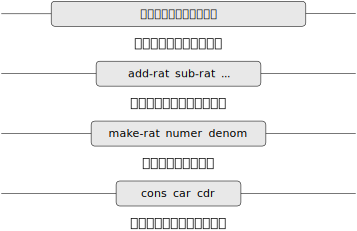
\includegraphics[width=91mm]{fig/chap2/Fig2.1c.pdf}
\begin{quote}
\heading{Figure 2.1:} Data-abstraction barriers in the rational-number package.
\end{quote}
\end{figure}

\noindent
For example, an alternate way to address the problem of reducing rational
numbers to lowest terms is to perform the reduction whenever we access the
parts of a rational number, rather than when we construct it.  This leads to
different constructor and selector procedures:

例として、分数を最小の項へと約分する問題の解法の代替法には、分数を組み立てた時でなく、
分数のパーツにアクセスする度に約分を実行する方法があります。
これは異なるコンストラクタとセレクタ手続に導きます。

\begin{scheme}
(define (make-rat n d) (cons n d))
(define (numer x)
  (let ((g (gcd (car x) (cdr x))))
    (/ (car x) g)))
(define (denom x)
  (let ((g (gcd (car x) (cdr x))))
    (/ (cdr x) g)))
\end{scheme}

\noindent
The difference between this implementation and the previous one lies in when we
compute the \code{gcd}.  If in our typical use of rational numbers we access
the numerators and denominators of the same rational numbers many times, it
would be preferable to compute the \code{gcd} when the rational numbers are
constructed.  If not, we may be better off waiting until access time to compute
the \code{gcd}.  In any case, when we change from one representation to the
other, the procedures \code{add\-/rat}, \code{sub\-/rat}, and so on do not have to
be modified at all.

この実装と依然の実装との間の違いはいつ\code{gcd}を求めるかにあります。
私達の典型的な分数の使用においては、同じ分数の分子と分母に何度もアクセスする場合、
分数が組み立てられる時に\code{gcd}を求めるほうが好ましいです。そうでなければ
\code{gcd}を求めるのはアクセスする時まで待ったほうが良いかもしれません。
どちらの場合でも、一方の表現からもう一方の表現へと変更する場合、手続、\code{add\-/rat}, 
\code{sub\-/rat}, その他は全く変更する必要がありません。

Constraining the dependence on the representation to a few interface procedures
helps us design programs as well as modify them, because it allows us to
maintain the flexibility to consider alternate implementations.  To continue
with our simple example, suppose we are designing a rational-number package and
we can't decide initially whether to perform the \code{gcd} at construction
time or at selection time.  The data-abstraction methodology gives us a way to
defer that decision without losing the ability to make progress on the rest of
the system.

表現上の依存対象を少ないインターフェイス手続に制約することはプログラムの設計と共に
それらの変更をも手助けします。なぜなら代替的な実装を考えるための柔軟性を保つ
ことを可能にするためです。私達の簡単な例で続けるために、私達は分数パッケージ
を設計中で、早期に\code{gcd}を構築時と選択時のどちらで実行するか決められないと
想像して下さい。データ抽象化メソドロジはその決定をシステムの他の部分上の進行の
可能性を失わせずに決定を遅らせる方法を与えます。

\begin{quote}
\heading{\phantomsection\label{Exercise 2.2}Exercise 2.2:} Consider the problem of
representing line segments in a plane.  Each segment is represented as a pair
of points: a starting point and an ending point.  Define a constructor
\code{make\-/segment} and selectors \code{start\-/segment} and \code{end\-/segment}
that define the representation of segments in terms of points.  Furthermore, a
point can be represented as a pair of numbers: the \( x \) coordinate and the
\( y \) coordinate.  Accordingly, specify a constructor \code{make\-/point} and
selectors \code{x\-/point} and \code{y\-/point} that define this representation.
Finally, using your selectors and constructors, define a procedure
\code{midpoint\-/segment} that takes a line segment as argument and returns its
midpoint (the point whose coordinates are the average of the coordinates of the
endpoints).  To try your procedures, you'll need a way to print points:

平面上の線分を表現する問題について考える。各線分は点のペアにて表現する。始点と
終点である。コンストラクタ\code{make\-/segment}とセレクタ\code{start\-/segment}と\code{end\-/segment}
を定義せよ。それらは点を用いて線分の表現を定義する。さらに点は数値のペアにて表現できる。
\( x \)座標と\( y \)座標である。それに沿ってこの表現を定義するコンストラクタ\code{make\-/point}と
セレクタ\code{x\-/point}を\code{y\-/point}を定めよ。
最後に、セレクタとコンストラクタを用いて引数として線分を取りその中点(その座標が両端点の
座標の平均である点)を返す手続\code{midpoint\-/segment}を定義せよ。
あなたの手続をテストするためには以下の点を表示する方法が必要だろう。

\begin{scheme}
(define (print-point p)
  (newline)
  (display "(")
  (display (x-point p))
  (display ",")
  (display (y-point p))
  (display ")"))
\end{scheme}
\end{quote}

\begin{quote}
\heading{\phantomsection\label{Exercise 2.3}Exercise 2.3:} Implement a representation for
rectangles in a plane.  (Hint: You may want to make use of \link{Exercise 2.2}.)
In terms of your constructors and selectors, create procedures that compute the
perimeter and the area of a given rectangle.  Now implement a different
representation for rectangles.  Can you design your system with suitable
abstraction barriers, so that the same perimeter and area procedures will work
using either representation?

平面上の長方形のための表現を実装せよ。(ヒント:\link{Exercise 2.2}を利用したいだろう。)
コンストラクタとセレクタを利用して、与えられた長方形の周辺の長さと面積を求める手続を
作れ。適切な抽象化バリアを用いてどんな表現を用いても同じ周辺長と面積の手続が働くよう、
あなたのシステムを設計できるだろうか?

\end{quote}

\label{Section 2.1.3}
\subsection{What Is Meant by Data?}

We began the rational-number implementation in \link{Section 2.1.1} by
implementing the rational-number operations \code{add\-/rat}, \code{sub\-/rat}, and
so on in terms of three unspecified procedures: \code{make\-/rat}, \code{numer},
and \code{denom}.  At that point, we could think of the operations as being
defined in terms of data objects---numerators, denominators, and rational
numbers---whose behavior was specified by the latter three procedures.


\link{Section 2.1.1}にて分数実装を分数演算\code{add\-/rat}, \code{sub\-/rat}, その他を
3つの定められていない手続、\code{make\-/rat}, \code{numer}, \code{denom}を用いて
実装することから始めました。その時点では命令はデータオブジェクト---分子、分母と
分数を用いて定義されると考えることができました。データオブジェクトの振舞は
後者の3つの手続により指定されました。

But exactly what is meant by \newterm{data}?  It is not enough to say
``whatever is implemented by the given selectors and constructors.''  Clearly,
not every arbitrary set of three procedures can serve as an appropriate basis
for the rational-number implementation.  We need to guarantee that, if we
construct a rational number \code{x} from a pair of integers \code{n} and
\code{d}, then extracting the \code{numer} and the \code{denom} of \code{x} and
dividing them should yield the same result as dividing \code{n} by \code{d}.
In other words, \code{make\-/rat}, \code{numer}, and \code{denom} must satisfy
the condition that, for any integer \code{n} and any non-zero integer \code{d},
if \code{x} is \code{(make\-/rat n d)}, then

しかし\newterm{data}(データ)とは正確には何を意味するのでしょうか。
``与えられたセレクタとコンストラクタにより実装された物全て''と言うのみでは十分ではありません。
明かに3つの手続の任意の集合全てが分数実装に対する適切な基準としての役割を果せる訳ではありません。
もし分数\code{x}を整数のペア\code{n}と\code{d}から組み立てた場合、\code{x}の\code{numer}と\code{denom}の抽出し
それらを割ることは、\code{n}を\code{d}で割るのと同じ結果になることを保証せねばなりません。
言い替えれば、\code{make\-/rat}, \code{numer}, \code{denom}は任意の整数\code{n}と零でない整数\code{d}に対し
もし\code{x}が\code{(make\-/rat n d)}である時、その場合以下の条件を満たさなければなりません。
\begin{comment}

\begin{example}
(numer x)    n
--------- = ---
(denom x)    d
\end{example}

\end{comment}
\begin{displaymath}
 {\hbox{\tt(numer x)} \over \hbox{\tt(denom x)}} = {{\tt n} \over {\tt d}}\,.  
\end{displaymath}
In fact, this is the only condition \code{make\-/rat}, \code{numer}, and
\code{denom} must fulfill in order to form a suitable basis for a
rational-number representation.  In general, we can think of data as defined by
some collection of selectors and constructors, together with specified
conditions that these procedures must fulfill in order to be a valid
representation.\footnote{Surprisingly, this idea is very difficult to formulate
rigorously. There are two approaches to giving such a formulation.  One,
pioneered by C. A. R. \link{Hoare (1972)}, is known as the method of \newterm{abstract
models}.  It formalizes the ``procedures plus conditions'' specification as
outlined in the rational-number example above.  Note that the condition on the
rational-number representation was stated in terms of facts about integers
(equality and division).  In general, abstract models define new kinds of data
objects in terms of previously defined types of data objects.  Assertions about
data objects can therefore be checked by reducing them to assertions about
previously defined data objects.  Another approach, introduced by Zilles at
\acronym{MIT}, by Goguen, Thatcher, Wagner, and Wright at IBM 
(see \link{Thatcher et al. 1978}), 
and by Guttag at Toronto (see \link{Guttag 1977}), is called
\newterm{algebraic specification}.  It regards the ``procedures'' as elements
of an abstract algebraic system whose behavior is specified by axioms that
correspond to our ``conditions,'' and uses the techniques of abstract algebra
to check assertions about data objects.  Both methods are surveyed in the paper
by \link{Liskov and Zilles (1975)}.}

実際にこれが\code{make\-/rat}, \code{numer}, \code{denom}が分数表現のための適切な基準を形成する
ために満たさなければならないただ1つの条件です。
一般的に、私達はデータをセレクタとコンストラクタのある集合と共に、これらの手続が
有効な表現となるために満たさなければならない制約により定義されると考えることができます。\footnote{
意外にもこの考えは厳格に形式化することがとても難しいのです。そのような形式化を与える試みは
2つあります。1つはC. A. R. \link{Hoare (1972)}により開拓され、\newterm{abstract models}(抽象モデル)
として知られています。``手続プラス制約''の仕様を上の分数の例内で概説されたように形式化します。
分数表現上の条件は整数に関する事実(等値関係と除算)を用いて規定されています。
一般的に抽象モデルは新しい種類のデータオブジェクトを以前に定義されたデータオブジェクトの型を用いて
定義します。従ってデータオブジェクトに関する成立条件はそれらを以前に定義されたデータオブジェクト
に関する成立条件へと還元していくことでチェックできます。
もう1つの試みは\acronym{MIT}のZillesとIBMのGoguen, Thatcher, Wagner, Wrightにより紹介され
(\link{Thatcher et al. 1978}を参照)、またトロント大学のGuttagにより紹介されました。(\link{Guttag 1977}
を参照)。その試みは``手続''を抽象代数システムの要素と見做し、その振舞は``条件''に相当する公理により
指定されました。そして抽象代数のテクニックを用いてデータオブジェクトに関する成立条件をチェックしました。
両者の手法が\link{Liskov and Zilles (1975)}により論文として調査されています。}

This point of view can serve to define not only ``high-level'' data objects,
such as rational numbers, but lower-level objects as well.  Consider the notion
of a pair, which we used in order to define our rational numbers.  We never
actually said what a pair was, only that the language supplied procedures
\code{cons}, \code{car}, and \code{cdr} for operating on pairs.  But the only
thing we need to know about these three operations is that if we glue two
objects together using \code{cons} we can retrieve the objects using \code{car}
and \code{cdr}.  That is, the operations satisfy the condition that, for any
objects \code{x} and \code{y}, if \code{z} is \code{(cons x y)} then \code{(car
z)} is \code{x} and \code{(cdr z)} is \code{y}.  Indeed, we mentioned that
these three procedures are included as primitives in our language.  However,
any triple of procedures that satisfies the above condition can be used as the
basis for implementing pairs.  This point is illustrated strikingly by the fact
that we could implement \code{cons}, \code{car}, and \code{cdr} without using
any data structures at all but only using procedures.  Here are the
definitions:

この視点は分数のような``高階データオブジェクト''のみを定義するのではなく、
より低いレベルのオブジェクトの定義も提供することができます。
私達が分数を定義するために使用したペアの概念について考えてみます。
私達はまだペアとは実際には何であるのか述べていません。言語が手続\code{cons}, \code{car}, \code{cdr}を
ペア上の命令として提供するとのみ説明しています。しかしこれら3つの命令について
知らなければいけないことはもし私達が2つのオブジェクトを\code{cons}を用いて貼り合わせた時、
\code{car}と\code{cdr}を用いてそれらのオブジェクトを取得することができることのみです。
つまり、それらの命令は任意のオブジェクト\code{x}と\code{y}に対し、もし\code{z}が\code{(cons x y)}であるなら
\code{(car z)}は\code{x}であり、\code{(cdr z)}は\code{y}であるという制約を満たしています。
実際に、これらの3つの手続は言語にプリミティブとして含まれていることについて既に述べました。
しかし、上記の制約を満たす任意の3つの手続ならペアを実装するための基盤として使用することが
可能です。この点は私達が\code{cons}, \code{car}, \code{cdr}をどんなデータ構造も全く利用せずに、
しかし手続のみを用いて実装できることにより、著しく説明されます。
これがその定義です。

\begin{scheme}
(define (cons x y)
  (define (dispatch m)
    (cond ((= m 0) x)
          ((= m 1) y)
          (else (error "Argument not 0 or 1: CONS" m))))
  dispatch)
(define (car z) (z 0))
(define (cdr z) (z 1))
\end{scheme}

\noindent
This use of procedures corresponds to nothing like our intuitive notion of what
data should be.  Nevertheless, all we need to do to show that this is a valid
way to represent pairs is to verify that these procedures satisfy the condition
given above.

この手続の使用はデータが何であるべきかという私達の直感的概念のような物には全く
関係しません。それでもなお、これがペアを表現するのに有効な方法であると示すのに
必要なこと全てはこれらの手続が上で与えられた制約を満たすことです。

The subtle point to notice is that the value returned by \code{(cons x y)} is a
procedure---namely the internally defined procedure \code{dispatch}, which
takes one argument and returns either \code{x} or \code{y} depending on whether
the argument is 0 or 1.  Correspondingly, \code{(car z)} is defined to apply
\code{z} to 0.  Hence, if \code{z} is the procedure formed by \code{(cons x
y)}, then \code{z} applied to 0 will yield \code{x}. Thus, we have shown that
\code{(car (cons x y))} yields \code{x}, as desired.  Similarly, \code{(cdr
(cons x y))} applies the procedure returned by \code{(cons x y)} to 1, which
returns \code{y}.  Therefore, this procedural implementation of pairs is a
valid implementation, and if we access pairs using only \code{cons},
\code{car}, and \code{cdr} we cannot distinguish this implementation from one
that uses ``real'' data structures.

注意すべき微細な点は\code{(cons x y)}により返される値は手続---すなわち内部で定義された
手続\code{dispatch}であることです。それが1つの引数を取り\code{x}か\code{y}のどちらかを
引数が0であるか1であるかに従って返します。相応して、\code{(car z)}は\code{z}を0に適用します。
故にもし\code{z}が\code{(cons x y)}により作られた手続であるのなら、\code{z}を0に適用すれば
\code{x}を返します。従って、\code{(car (cons x y))}が希望通りに\code{x}を返すことを示しました。
同様に\code{(cdr (cons x y))}は\code{(cons x y)}の返り値としての手続を1に適用し、
\code{y}を返します。従ってこのペアの手続としての実装は有効な実装であり、もし私達が
\code{cons}, \code{car}, \code{cdr}のみを用いてペアにアクセスする場合、この実装を``本物の''データ構造を
用いる実装と区別することはできません。

The point of exhibiting the procedural representation of pairs is not that our
language works this way (Scheme, and Lisp systems in general, implement pairs
directly, for efficiency reasons) but that it could work this way.  The
procedural representation, although obscure, is a perfectly adequate way to
represent pairs, since it fulfills the only conditions that pairs need to
fulfill.  This example also demonstrates that the ability to manipulate
procedures as objects automatically provides the ability to represent compound
data.  This may seem a curiosity now, but procedural representations of data
will play a central role in our programming repertoire.  This style of
programming is often called \newterm{message passing}, and we will be using it
as a basic tool in \link{Chapter 3} when we address the issues of modeling and
simulation.

ペアの手続による表現を提示することのポイントは私達の言語がこのように働いているという
ことではなく(Schemeや一般的なLispシステムは効率上の理由からペアを直接的に実装します)、
しかしそれがこのように働くことができるということです。手続による表現は曖昧ですが、ペアを
表現するのに完璧に適切な方法です。ペアが満たすべき必要な条件を満たすからです。
この例はまた手続をオブジェクトとして操作する能力が自動的に複合データを表現する能力を
提供することを実演しました。これは今は珍しく見えるかもしれませんが、しかし手続による
データの表現は私達のプログラミングレパートリの中心的役割を演じます。このプログラミング
スタイルは時折\newterm{message passing}(メッセージパッシング)と呼ばれ、私達はこれを
\link{Chapter 3}にてモデリングとシミュレーションの問題を解決する時に基本的なツールとして
用います。

\begin{quote}
\heading{\phantomsection\label{Exercise 2.4}Exercise 2.4:} Here is an alternative procedural
representation of pairs.  For this representation, verify that \code{(car (cons
x y))} yields \code{x} for any objects \code{x} and \code{y}.

ここにペアの代替的な手続上の表現がある。この表現に対して\code{(car (cons
x y))}が任意のオブジェクト\code{x}と\code{y}に対して\code{x}を返すか確認せよ。

\begin{scheme}
(define (cons x y)
  (lambda (m) (m x y)))
(define (car z)
  (z (lambda (p q) p)))
\end{scheme}

What is the corresponding definition of \code{cdr}? (Hint: To verify that this
works, make use of the substitution model of \link{Section 1.1.5}.)

対応する\code{cdr}の定義はどうなるか? (ヒント:これが正しく働くか確認するには
\link{Section 1.1.5}の置換モデルを使用せよ)
\end{quote}

\begin{quote}
\heading{\phantomsection\label{Exercise 2.5}Exercise 2.5:} Show that we can represent pairs of
nonnegative integers using only numbers and arithmetic operations if we
represent the pair \( a \) and \( b \) as the integer that is the product \( 2^a 3^b \).  
Give the corresponding definitions of the procedures \code{cons},
\code{car}, and \code{cdr}.

負ではない整数のペアを数値と数値演算命令のみを用いて表現できることを、もし\( a \)と\( b \)の
ペアを積\( 2^a 3^b \)の整数で表現すれば可能であることにより示せ。
対応する手続\code{cons}, \code{car}, \code{cdr}.の定義を与えよ。
\end{quote}

\begin{quote}
\heading{\phantomsection\label{Exercise 2.6}Exercise 2.6:} In case representing pairs as
procedures wasn't mind-boggling enough, consider that, in a language that can
manipulate procedures, we can get by without numbers (at least insofar as
nonnegative integers are concerned) by implementing 0 and the operation of
adding 1 as

ペアを手続として表現することが十分に驚かせるに値するものでない場合、
手続を操作可能なある言語においては0と1を足すことを以下のように実装することで
数値が無くてもやっていける(少なくとも負ではない整数のみを考える場合においては)ことを
考えてみよ。

\begin{scheme}
(define zero (lambda (f) (lambda (x) x)))
(define (add-1 n)
  (lambda (f) (lambda (x) (f ((n f) x)))))
\end{scheme}

This representation is known as \newterm{Church numerals}, after its inventor,
Alonzo Church, the logician who invented the \( \lambda \)-calculus.

この表現はその開発者に因んで\newterm{Church numerals}(チャーチ数)として知られる。
Alonzo Churchは\( \lambda \)-演算を発明した論理学者である。

Define \code{one} and \code{two} directly (not in terms of \code{zero} and
\code{add\-/1}).  (Hint: Use substitution to evaluate \code{(add\-/1 zero)}).  Give
a direct definition of the addition procedure \code{+} (not in terms of
repeated application of \code{add\-/1}).

\code{one}と\code{two}を直接(\code{zero}と\code{add\-/1}を用いずに)定義せよ。(ヒント:
加算手続の直接的な定義\code{+}を与えよ。(\code{add\-/1}の繰り返し適用は用いない)
\end{quote}


\label{Section 2.1.4}
\subsection{Extended Exercise: Interval Arithmetic}

Alyssa P. Hacker is designing a system to help people solve engineering
problems.  One feature she wants to provide in her system is the ability to
manipulate inexact quantities (such as measured parameters of physical devices)
with known precision, so that when computations are done with such approximate
quantities the results will be numbers of known precision.

Alyssa P. Hackerは人々が工学上の問題を解くのを手助けするシステムを設計しています。
システムにおいて彼女が提供したい1つの機能は(物理機器の測定されたパラメータのような)不正確な量を
既知の精度にて扱う能力です。演算がそのような近似量にて行われた時、結果が既知の
精度の値になるようにするためです。

Electrical engineers will be using Alyssa's system to compute electrical
quantities.  It is sometimes necessary for them to compute the value of a
parallel equivalent resistance \( R_p \) of two resistors \( R_1 \), \( R_2 \)
using the formula

電気技術者達がAlyssaのシステムを電気の量を計算するために使用します。彼らは時折2つの
抵抗\( R_1 \), \( R_2 \)の並列に等価な抵抗値\( R_p \)を次の式を用いて計算する
必要があります。
\begin{comment}

\begin{example}
            1
R_p = -------------
      1/R_1 + 1/R_2
\end{example}

\end{comment}
\begin{displaymath}
 R_p = {1 \over 1 / R_1 + 1 / R_2}\,.
\end{displaymath}
Resistance values are usually known only up to some tolerance guaranteed by the
manufacturer of the resistor.  For example, if you buy a resistor labeled ``6.8
ohms with 10\% tolerance'' you can only be sure that the resistor has a
resistance between \( 6.8 - 0.68 = 6.12 \) and \( 6.8 + 0.68 = 7.48 \) ohms.  Thus, if you
have a 6.8-ohm 10\% resistor in parallel with a 4.7-ohm 5\% resistor, the
resistance of the combination can range from about 2.58 ohms (if the two
resistors are at the lower bounds) to about 2.97 ohms (if the two resistors are
at the upper bounds).

抵抗値は通常抵抗の生産者により保証されるいくらかの許容誤差未満であることが知られています。
例えばもしあなたが``10\%の許容誤差で6.8Ω''とラベリングされた抵抗を買ったとしたら、
確かなのはその抵抗は\( 6.8 - 0.68 = 6.12 \)と\( 6.8 + 0.68 = 7.48 \)Ωの間の抵抗を
持つことのみです。従って、もし6.8Ω 10\%の抵抗と並列に4.7Ω 5\%の抵抗を接続した場合に、
組み合わせの抵抗は約2.58Ω(2つの抵抗が低限である場合)から約2.97Ω(2つの抵抗が上限である場合)
の区間になります。

Alyssa's idea is to implement ``interval arithmetic'' as a set of arithmetic
operations for combining ``intervals'' (objects that represent the range of
possible values of an inexact quantity).  The result of adding, subtracting,
multiplying, or dividing two intervals is itself an interval, representing the
range of the result.

Alyssaのアイデアは``interval arithmetic''(区間演算)を``区間''(不正確な量の取り得る
値の区間を表現するオブジェクト)を連結する演算命令の集合として実装することです。
2つの区間の加算、減算、乗算、除算の結果はそれ自身が区間であり、結果の範囲を表します。

Alyssa postulates the existence of an abstract object called an ``interval''
that has two endpoints: a lower bound and an upper bound.  She also presumes
that, given the endpoints of an interval, she can construct the interval using
the data constructor \code{make\-/interval}.  Alyssa first writes a procedure for
adding two intervals.  She reasons that the minimum value the sum could be is
the sum of the two lower bounds and the maximum value it could be is the sum of
the two upper bounds:

Alyssaは2つの終端、下限と上限を持つ``区間''と呼ばれる抽象オブジェクトの存在を仮定しました。
彼女はまた区間の終端を与えられた時、データコンストラクタ\code{make\-/interval}を用いて区間の
構築ができると仮定しました。Alyssaは最初に2つの区間を足す手続を書きました。彼女は和の最小値は
2つの下限の和であり、最大値は2つの上限の和になるだろうと推測しました。

\begin{scheme}
(define (add-interval x y)
  (make-interval (+ (lower-bound x) (lower-bound y))
                 (+ (upper-bound x) (upper-bound y))))
\end{scheme}

\noindent
Alyssa also works out the product of two intervals by finding the minimum and
the maximum of the products of the bounds and using them as the bounds of the
resulting interval.  (\code{Min} and \code{max} are primitives that find the
minimum or maximum of any number of arguments.)

Alyssaはまた2つの区間の積を限界値の積の最小値と最大値を見つけることで算出し、
そしてそれらを結果区間の限界値として用いました。(\code{min}と\code{max}は任意の数の引数の
最小値と最大値を見つけるプリミティブです)。

\begin{scheme}
(define (mul-interval x y)
  (let ((p1 (* (lower-bound x) (lower-bound y)))
        (p2 (* (lower-bound x) (upper-bound y)))
        (p3 (* (upper-bound x) (lower-bound y)))
        (p4 (* (upper-bound x) (upper-bound y))))
    (make-interval (min p1 p2 p3 p4)
                   (max p1 p2 p3 p4))))
\end{scheme}

\noindent
To divide two intervals, Alyssa multiplies the first by the reciprocal of the
second.  Note that the bounds of the reciprocal interval are the reciprocal of
the upper bound and the reciprocal of the lower bound, in that order.

2つの区間を割るために、Alyssaは一つ目に2つ目の逆数を掛けました。区間の逆数の限界値は
上限の逆数と下限の逆数をその順で用いることに注意して下さい。

\begin{scheme}
(define (div-interval x y)
  (mul-interval 
   x
   (make-interval (/ 1.0 (upper-bound y))
                  (/ 1.0 (lower-bound y)))))
\end{scheme}

\begin{quote}
\heading{\phantomsection\label{Exercise 2.7}Exercise 2.7:} Alyssa's program is incomplete
because she has not specified the implementation of the interval abstraction.
Here is a definition of the interval constructor:

Alyssaのプログラムは未完成である。なぜなら彼女は区間の抽象の実装を特定していない。
ここに区間のコンストラクタの定義を置く。

\begin{scheme}
(define (make-interval a b) (cons a b))
\end{scheme}

Define selectors \code{upper\-/bound} and \code{lower\-/bound} to complete the
implementation.

セレクタ\code{upper\-/bound}と\code{lower\-/bound}を定義し実装を完成させよ。
\end{quote}

\begin{quote}
\heading{\phantomsection\label{Exercise 2.8}Exercise 2.8:} Using reasoning analogous to
Alyssa's, describe how the difference of two intervals may be computed.  Define
a corresponding subtraction procedure, called \code{sub\-/interval}.

Alyssaの考えと同様の推論を用いて、2つの区間の差がどのように計算されるかを説明せよ。
対応する減算手続\code{sub\-/interval}を定義せよ。
\end{quote}

\begin{quote}
\heading{\phantomsection\label{Exercise 2.9}Exercise 2.9:} The \newterm{width} of an interval
is half of the difference between its upper and lower bounds.  The width is a
measure of the uncertainty of the number specified by the interval.  For some
arithmetic operations the width of the result of combining two intervals is a
function only of the widths of the argument intervals, whereas for others the
width of the combination is not a function of the widths of the argument
intervals.  Show that the width of the sum (or difference) of two intervals is
a function only of the widths of the intervals being added (or subtracted).
Give examples to show that this is not true for multiplication or division.

区間の\newterm{width}(幅)は上限と下限の差の半値である。幅は区間で指定された数値
の不確かさの基準である。いくつかの数値演算に対しては、2つの区間を結合した結果の幅は
引数区間の幅のみによる関数である。一方で他の演算においては結合の幅は引数の幅の
関数ではない。2つの区間の和、または差の幅は足される、または引かれる区間の幅の
関数であることを示せ。これが乗算と除算においては正しくないことを例をもって示せ。
\end{quote}

\begin{quote}
\heading{\phantomsection\label{Exercise 2.10}Exercise 2.10:} Ben Bitdiddle, an expert systems
programmer, looks over Alyssa's shoulder and comments that it is not clear what
it means to divide by an interval that spans zero.  Modify Alyssa's code to
check for this condition and to signal an error if it occurs.

エキスパートシステムプログラマのBen BitdiddleはAlyssaの肩越しに覗いて、
区間の長さが0の時に割ったらどうなるのか不明だよとコメントした。
Alyssaのコードを変更し、この条件をチェックしてもしそれが起こればエラーを返すようにせよ。
\end{quote}

\begin{quote}
\heading{\phantomsection\label{Exercise 2.11}Exercise 2.11:} In passing, Ben also cryptically
comments: ``By testing the signs of the endpoints of the intervals, it is
possible to break \code{mul\-/interval} into nine cases, only one of which
requires more than two multiplications.''  Rewrite this procedure using Ben's
suggestion.

通り過ぎながらBenはまた曖昧なコメントを残した。``区間の終端の符号をテストすることで
\code{mul\-/interval}を7つに場合分けできる。その1つのみが2つ以上の乗算を必要とする。''
この手続をBenの提案に従い書き直せ。
\end{quote}
\noindent
After debugging her program, Alyssa shows it to a potential user, who complains
that her program solves the wrong problem.  He wants a program that can deal
with numbers represented as a center value and an additive tolerance; for
example, he wants to work with intervals such as \( 3.5 \pm 0.15 \) rather than
[3.35, 3.65].  Alyssa returns to her desk and fixes this problem by supplying
an alternate constructor and alternate selectors:

プログラムをデバッグした後で、Alyssaはユーザ候補の一人に見せた。彼は彼女の
プログラムは間違った問題を解いていると文句を言った。彼が欲しい のは中央値として
表現された数値と追加の許容誤差を扱えるプログラムだ。例えば彼は\( 3.5 \pm 0.15 \)の
ような区間を扱いたく、[3.35, 3.65]ではない。Alyssaは彼女の机に戻りこの問題を代替となる
コンストラクタとセレクタを提供することで直した。

\begin{scheme}
(define (make-center-width c w)
  (make-interval (- c w) (+ c w)))
(define (center i)
  (/ (+ (lower-bound i) (upper-bound i)) 2))
(define (width i)
  (/ (- (upper-bound i) (lower-bound i)) 2))
\end{scheme}
\noindent
Unfortunately, most of Alyssa's users are engineers.  Real engineering
situations usually involve measurements with only a small uncertainty, measured
as the ratio of the width of the interval to the midpoint of the interval.
Engineers usually specify percentage tolerances on the parameters of devices,
as in the resistor specifications given earlier.

不運なことに、Alyssaのユーザの多くはエンジニアです。実際の工学の場では通常、小さな不確かさ
を伴なう計測を伴い、区間の中央値に対する区間の幅の割合として測定されます。
エンジニアは通常パーセンテージにて許容誤差を端末のパラメータ上に、以前に与えた抵抗の
仕様のように指定します。

\begin{quote}
\heading{\phantomsection\label{Exercise 2.12}Exercise 2.12:} Define a constructor
\code{make\-/center\-/percent} that takes a center and a percentage tolerance and
produces the desired interval.  You must also define a selector \code{percent}
that produces the percentage tolerance for a given interval.  The \code{center}
selector is the same as the one shown above.

コンストラクタ\code{make\-/center\-/percent}を中央値とパーセンテージ許容誤差を取り
望まれた区間を返すように定義せよ。セレクタ\code{percent}を与えられた区間に対する
パーセンテージ許容誤差を返すように定義することも行うこと。\code{center}セレクタは
上で見たものと同じである。
\end{quote}

\begin{quote}
\heading{\phantomsection\label{Exercise 2.13}Exercise 2.13:} Show that under the assumption of
small percentage tolerances there is a simple formula for the approximate
percentage tolerance of the product of two intervals in terms of the tolerances
of the factors.  You may simplify the problem by assuming that all numbers are
positive.

小さなパーセンテージ許容誤差の前提の下では、2つの区間の積のパーセンテージ許容誤差を
因数の許容誤差を用いて近似するための簡単な式が存在することを示せ。
全ての数値は正であると前提して問題を簡単にしても良い。
\end{quote}

\noindent
After considerable work, Alyssa P. Hacker delivers her finished system.
Several years later, after she has forgotten all about it, she gets a frenzied
call from an irate user, Lem E. Tweakit.  It seems that Lem has noticed that
the formula for parallel resistors can be written in two algebraically
equivalent ways:

大変な仕事を終え、Alyssa P. Hackerは完了したシステムを受け渡しました。何年か後、彼女が全てを忘れた頃に、
彼女は興奮した電話を、怒ったユーザ、Lem E. Tweakitから受けました。どうやらLemは並列接続の抵抗の式が2つの
代数的に等価な方法で書くことができることに気付いたようです。
\begin{comment}

\begin{example}
 R_1 R_2
---------
R_1 + R_2
\end{example}

\end{comment}
\begin{displaymath}
 R_1 R_2 \over R_1 + R_2 
\end{displaymath}
\noindent
and
\begin{comment}

\begin{example}
      1
-------------
1/R_1 + 1/R_2
\end{example}

\end{comment}
\begin{displaymath}
 {1 \over 1 / R_1 + 1 / R_2}\,. 
\end{displaymath}
He has written the following two programs, each of which computes the
parallel-resistors formula differently:

彼は以下の2つのプログラムを書きました。それぞれが並列接続の抵抗値を異なる式で計算します。

\begin{scheme}
(define (par1 r1 r2)
  (div-interval (mul-interval r1 r2)
                (add-interval r1 r2)))
\end{scheme}

\begin{scheme}
(define (par2 r1 r2)
  (let ((one (make-interval 1 1)))
    (div-interval 
     one (add-interval (div-interval one r1)
                       (div-interval one r2)))))
\end{scheme}

\vspace{0.3em}

Lem complains that Alyssa's program gives different answers for the two ways of
computing. This is a serious complaint.

LemはAlyssaのプログラムは2つの方法の演算にて異なる値を返すと抗議しました。
これは深刻な苦情です。

\begin{quote}
\heading{\phantomsection\label{Exercise 2.14}Exercise 2.14:} Demonstrate that Lem is right.
Investigate the behavior of the system on a variety of arithmetic
expressions. Make some intervals \( A \) and \( B \), and use them in computing the
expressions \( A \big/\! A \) and \( A \big/\! B \).  You will get the most insight by
using intervals whose width is a small percentage of the center value. Examine
the results of the computation in center-percent form (see \link{Exercise 2.12}).

Lemが正しいことを確認せよ。様々な数値演算にてシステムの挙動を調べよ。
ある区間\( A \)と\( B \)を作成し、式\( A /\! A \)と\( A / B \)の計算において
それらを用いよ。幅が中央値の小さなパーセンテージである区間を用いることで多くの実態を掴む
ことができるだろう。center-percent形式(\link{Exercise 2.12}参照)の演算の結果を
調査せよ。
\end{quote}

\begin{quote}
\heading{\phantomsection\label{Exercise 2.15}Exercise 2.15:} Eva Lu Ator, another user, has
also noticed the different intervals computed by different but algebraically
equivalent expressions. She says that a formula to compute with intervals using
Alyssa's system will produce tighter error bounds if it can be written in such
a form that no variable that represents an uncertain number is repeated.  Thus,
she says, \code{par2} is a ``better'' program for parallel resistances than
\code{par1}.  Is she right?  Why?

Eva Lu Atorはもう一人のユーザで、彼女もまた異なるが代数的には等価な式により異なる区間が
算出されることに気付いた。彼女はAlyssaのシステムを用いて区間の計算をする式が、
もし式が不確かな値を表現する変数がどれも繰り返されない形であれば、より厳しい
エラーの限界を算出すると言う。
従って彼女は抵抗の並列に対し、\code{par2}の方が\code{par1}より``より良い''プログラムであると述べた。
彼女は正しいだろうか? それは何故か?
\end{quote}

\begin{quote}
\heading{\phantomsection\label{Exercise 2.16}Exercise 2.16:} Explain, in general, why
equivalent algebraic expressions may lead to different answers.  Can you devise
an interval-arithmetic package that does not have this shortcoming, or is this
task impossible?  (Warning: This problem is very difficult.)

一般的に、なぜ等価な代数式が異なる答に導くのか説明せよ。
この欠点を持たない区間演算パッケージを開発することは可能だろうか。
または不可能だろうか。(警告:この問題はとても難しい)
\end{quote}

%=======================================================================================================

\label{Section 2.2}
\section{Hierarchical Data and the Closure Property}

As we have seen, pairs provide a primitive ``glue'' that we can use to
construct compound data objects.  \link{Figure 2.2} shows a standard way to
visualize a pair---in this case, the pair formed by \code{(cons 1 2)}.  In this
representation, which is called \newterm{box-and-pointer notation}, each object
is shown as a \newterm{pointer} to a box.  The box for a primitive object
contains a representation of the object.  For example, the box for a number
contains a numeral.  The box for a pair is actually a double box, the left part
containing (a pointer to) the \code{car} of the pair and the right part
containing the \code{cdr}.

ここまで学んだように、ペアは私達が複合データオブジェクトを構築するのに利用可能な
プリミティブな``糊''を提供する。\link{Figure 2.2}はペア---この場合は\code{(cons 1 2)}
にて形成されたペアを図示する標準的な方法を示している。
この\newterm{box-and-pointer notation}(箱と点表記法)と呼ばれる表現において、
各オブジェクトは箱への\newterm{pointer}(ポインタ)として表わされている。
プリミティブオブジェクトの箱はオブジェクトの表現を持っている。例えば数値の箱は
数字を持っている。ペアの箱は実際には二重の箱で、左部分はペアの\code{car}(へのポインタ)
を持っており、右部分は\code{cdr}を持っている。


We have already seen that \code{cons} can be used to combine not only numbers
but pairs as well.  (You made use of this fact, or should have, in doing
\link{Exercise 2.2} and \link{Exercise 2.3}.)  As a consequence, pairs provide a
universal building block from which we can construct all sorts of data
structures.  \link{Figure 2.3} shows two ways to use pairs to combine the
numbers 1, 2, 3, and 4.

私達は既に\code{cons}が数値のみでなくペアもまた組み合わせられることについて学びました。
(\link{Exercise 2.2}と\link{Exercise 2.3}であなたはこの事実を用いたか、または用いざるを得な
かったでしょう)。結果としてペアは全ての種類のデータ構造を構築可能な普遍的な構築ブロックを
提供します。\link{Figure 2.3}は数値1, 2, 3, 4を組み合わせるためにペアを用いる
2つの方法を示しています。

\begin{figure}[tb]
\phantomsection\label{Figure 2.2}
\centering
\begin{comment}
\heading{Figure 2.2:} Box-and-pointer representation of \code{(cons 1 2)}.

\begin{example}
     +---+---+     +---+
---->| * | *-+---->| 2 |
     +-|-+---+     +---+
       |
       V
     +---+
     | 1 |
     +---+
\end{example}
\end{comment}
\includegraphics[width=34mm]{fig/chap2/Fig2.2c.pdf}
\begin{quote}
\heading{Figure 2.2:} Box-and-pointer representation of \code{(cons 1 2)}.
\end{quote}
\end{figure}

\begin{figure}[tb]
\phantomsection\label{Figure 2.3}
\centering
\begin{comment}
\heading{Figure 2.3:} Two ways to combine 1, 2, 3, and 4 using pairs.

\begin{example}
     +---+---+     +---+---+         +---+---+     +---+
---->| * | *-+---->| * | * |    ---->| * | *-+---->| 4 |
     +-|-+---+     +-|-+-|-+         +-|-+---+     +---+
       |             |   |             |
       V             V   V             V
   +---+---+      +---+ +---+      +---+---+     +---+---+
   | * | * |      | 3 | | 4 |      | * | *-+---->| * | * |
   +-|-+-|-+      +---+ +---+      +-|-+---+     +-|-+-|-+
     |   |                           |             |   |
     V   V                           V             V   V
  +---+ +---+                      +---+        +---+ +---+
  | 1 | | 2 |                      | 1 |        | 2 | | 3 |
  +---+ +---+                      +---+        +---+ +---+

  (cons (cons 1 2)                 (cons (cons 1
        (cons 3 4))                            (cons 2 3))
                                         4)
\end{example}
\end{comment}
\includegraphics[width=96mm]{fig/chap2/Fig2.3c.pdf}
\begin{quote}
\heading{Figure 2.3:} Two ways to combine 1, 2, 3, and 4 using pairs.
\end{quote}
\end{figure}

\noindent
The ability to create pairs whose elements are pairs is the essence of list
structure's importance as a representational tool.  We refer to this ability as
the \newterm{closure property} of \code{cons}.  In general, an operation for
combining data objects satisfies the closure property if the results of
combining things with that operation can themselves be combined using the same
operation.\footnote{The use of the word ``closure'' here comes from abstract
algebra, where a set of elements is said to be closed under an operation if
applying the operation to elements in the set produces an element that is again
an element of the set.  The Lisp community also (unfortunately) uses the word
``closure'' to describe a totally unrelated concept: A closure is an
implementation technique for representing procedures with free variables.  We
do not use the word ``closure'' in this second sense in this book.  } Closure
is the key to power in any means of combination because it permits us to create
\newterm{hierarchical} structures---structures made up of parts, which
themselves are made up of parts, and so on.

要素がペアであるペアを作成する能力は表現ツールとしてのリスト構造の重要性の本質です。
私達はこの能力を\code{cons}の\newterm{閉包性}(closure property)と呼びます。
一般的に、データオブジェクトを組み合わせる操作は
もしその命令による組み合わせの結果それ自身が同じ命令を用いて組み合わせることが可能ならば
閉包性を満たします。\footnote{
ここでの``closure''(閉包)という用語の使用は抽象代数から来ており、
もし操作の集合の要素への適用により生成される要素が再び同じ集合の要素である場合、
要素の集合が操作の下において閉じられていると呼ばれます。Lispコミュニティでは(残念なことに)
用語``closure''を全く関係のない概念にも使用しています。closureとは自由変数を持つ
手続を表現するための実装テクニックです。私達は``closure''をこの本の中では2つ目の意味では
用いません。}
閉包はどのような目的の組み合わせをも強力にする鍵となります。なぜなら\newterm{hierarchical}(階層)構造---
複数のパーツから成る構造であり、パーツ自身も複数のパーツから成るような構造を作成することが
可能になるためです。

From the outset of \link{Chapter 1}, we've made essential use of closure in
dealing with procedures, because all but the very simplest programs rely on the
fact that the elements of a combination can themselves be combinations.  In
this section, we take up the consequences of closure for compound data.  We
describe some conventional techniques for using pairs to represent sequences
and trees, and we exhibit a graphics language that illustrates closure in a
vivid way.\footnote{The notion that a means of combination should satisfy
closure is a straightforward idea.  Unfortunately, the data combiners provided
in many popular programming languages do not satisfy closure, or make closure
cumbersome to exploit.  In Fortran or Basic, one typically combines data
elements by assembling them into arrays---but one cannot form arrays whose
elements are themselves arrays.  Pascal and C admit structures whose elements
are structures.  However, this requires that the programmer manipulate pointers
explicitly, and adhere to the restriction that each field of a structure can
contain only elements of a prespecified form.  Unlike Lisp with its pairs,
these languages have no built-in general-purpose glue that makes it easy to
manipulate compound data in a uniform way.  This limitation lies behind Alan
Perlis's comment in his foreword to this book: ``In Pascal the plethora of
declarable data structures induces a specialization within functions that
inhibits and penalizes casual cooperation.  It is better to have 100 functions
operate on one data structure than to have 10 functions operate on 10 data
structures.''}

\link{Chapter 1}の始めから、手続の取扱において閉包を本質的に利用してきました。
とても簡単なプログラムを除けば全てのプログラムは組み合わせの要素はそれ自身も
また組み合わせであるという事実に依存しているためです。
この節では複合データにとっての閉包の重要性を取り上げます。
ペアを使用して列と木を表現するための、いくつかの便利なテクニックを説明します。
そして鮮烈な方法でクロージャを図示するグラフィック言語を提示します。\footnote{
組み合わせは閉包であるべきだという手段の概念は単純なアイデアです。
残念なことに多くの人気の有るプログラミング言語が提供するデータの組み合わせ手法は
閉包性を満たしませんし、閉包性の活用が面倒です。FortranやBASICではデータ要素を
組合せる典型的な1つの手段は配列にそれらをまとめることです。しかし配列の要素自身が
配列である配列を形成できません。PascalとCは構造体の要素が構造体であることを認めます。
しかしこれはプログラマが明示的にポインタを取り扱うことを要求し、構造体の各フィールドが
事前に指定された形式の要素のみを保管できるという制約に帰着します。Lispのペアとは
異なりこれらの言語は複合データを統一的な方法で扱うことを簡単にする組み込みの汎用目的な糊
を持っていません。この制約がこの本の前書きにおけるAlan Perlisのコメントの背景にあります。
``Pascalにおける過剰な宣言可能なデータ構造は関数内にて特殊化を引き起こし、カジュアルな連携を
不利にし、抑制してしまう。1つのデータ構造を操作する100の関数を持つほうが、10のデータ構造を
操作する10の関数を持つよりも良い。''}

\label{Section 2.2.1}
\subsection{Representing Sequences}

One of the useful structures we can build with pairs is a
\newterm{sequence}---an ordered collection of data objects.  There are, of
course, many ways to represent sequences in terms of pairs.  One particularly
straightforward representation is illustrated in \link{Figure 2.4}, where the
sequence 1, 2, 3, 4 is represented as a chain of pairs.  The \code{car} of each
pair is the corresponding item in the chain, and the \code{cdr} of the pair is
the next pair in the chain.  The \code{cdr} of the final pair signals the end
of the sequence by pointing to a distinguished value that is not a pair,
represented in box-and-pointer diagrams as a diagonal line and in programs as
the value of the variable \code{nil}.  The entire sequence is constructed by
nested \code{cons} operations:

ペアを用いて構築可能な便利な構造の1つが\newterm{sequence}(列)---順に並べたデータ
オブジェクトの集合です。もちろんペアを用いて列を表現する方法は数多く存在します。
特に簡単な表現方法の1つを\link{Figure 2.4}に示します。列1, 2, 3, 4がペアの連鎖として
表わされています。各ペアの\code{car}は鎖内で相対するアイテムであり、各ペアの\code{cdr}は
鎖内での次のペアです。最後のペアの\code{cdr}は列の終端をペアではないことを識別する値を
指し示すことで合図します。箱とポインタの図では斜めの線にて表現され、プログラムでは
変数\code{nil}の値にて示されます。列全体は入れ子の\code{cons}命令にて構築されます。

\begin{scheme}
(cons 1
      (cons 2
            (cons 3
                  (cons 4 nil))))
\end{scheme}

\begin{figure}[tb]
\phantomsection\label{Figure 2.4}
\centering
\begin{comment}
\heading{Figure 2.4:} The sequence 1, 2, 3, 4 represented as a chain of pairs.

\begin{example}
     +---+---+     +---+---+     +---+---+     +---+---+
---->| * | *-+---->| * | *-+---->| * | *-+---->| * | / |
     +-|-+---+     +-|-+---+     +-|-+---+     +-|-+---+
       |             |             |             |
       V             V             V             V
     +---+         +---+         +---+         +---+
     | 1 |         | 2 |         | 3 |         | 4 |
     +---+         +---+         +---+         +---+
\end{example}
\end{comment}
\includegraphics[width=76mm]{fig/chap2/Fig2.4c.pdf}
\begin{quote}
\heading{Figure 2.4:} The sequence 1, 2, 3, 4 represented as a chain of pairs.
\end{quote}
\end{figure}

\noindent
Such a sequence of pairs, formed by nested \code{cons}es, is called a
\newterm{list}, and Scheme provides a primitive called \code{list} to help in
constructing lists.\footnote{In this book, we use \newterm{list} to mean a
chain of pairs terminated by the end-of-list marker.  In contrast, the term
\newterm{list structure} refers to any data structure made out of pairs, not
just to lists.}  The above sequence could be produced by \code{(list 1 2 3 4)}.
In general,

そのようなペアの列は入れ子の\code{cons}にて形成され、\newterm{list}(リスト)と呼ばれます。
そしてSchemeは\code{list}と呼ばれるプリミティブを提供しリストの構築を手助けします。\footnote{
この本では\newterm{list}をリスト終端マーカーにて終端化されたペアの鎖を意味するように
使用します。一方で用語\newterm{list structure}(リスト構造)はペアから作り上げられた
任意のデータ構造を参照し、ただのリストは意味しません。}
上の列は\code{(list 1 2 3 4)}により生成可能です。

\begin{scheme}
(list ~\( \dark \langle \)~~\( \dark a_1 \)~~\( \dark \rangle \)~ ~\( \dark \langle \)~~\( \dark a_2 \)~~\( \dark \rangle \)~ ~\( \dots \)~ ~\( \dark \langle \)~~\( \dark a_n \)~~\( \dark \rangle \)~)
\end{scheme}

\noindent
is equivalent to

は以下と等価です。

\begin{scheme}
(cons ~\( \dark \langle \)~~\( \dark a_1 \)~~\( \dark \rangle \)~
      (cons ~\( \dark \langle \)~~\( \dark a_2 \)~~\( \dark \rangle \)~
            (cons ~\( \dots \)~
                  (cons ~\( \dark \langle \)~~\( \dark a_n \)~~\( \dark \rangle \)~
                        nil)~\( \dots \)~)))
\end{scheme}

\noindent
Lisp systems conventionally print lists by printing the sequence of elements,
enclosed in parentheses.  Thus, the data object in \link{Figure 2.4} is printed
as \code{(1 2 3 4)}:

Lispシステムは慣習としてリストを括弧で括られた要素の列を表示することで表します。
従って\link{Figure 2.4}のデータオブジェクトは\code{(1 2 3 4)}の様に表示されます。

\begin{scheme}
(define one-through-four (list 1 2 3 4))
one-through-four
~\textit{(1 2 3 4)}~
\end{scheme}

\noindent
Be careful not to confuse the expression \code{(list 1 2 3 4)} with the list
\mbox{\code{(1 2 3 4)}}, which is the result obtained when the expression is
evaluated.  Attempting to evaluate the expression \code{(1 2 3 4)} will signal
an error when the interpreter tries to apply the procedure \code{1} to
arguments \code{2}, \code{3}, and \code{4}.

式\code{(list 1 2 3 4)}とリスト\mbox{\code{(1 2 3 4)}}を取り違えないよう気をつけて下さい。
リストは式が評価された時に得られた結果です。式\code{(1 2 3 4)}を評価しようとする試みは
インタプリタが手続\code{1}を引数\code{2}, \code{3}, \code{4}に適用しようとした時にエラーを
発します。

We can think of \code{car} as selecting the first item in the list, and of
\code{cdr} as selecting the sublist consisting of all but the first item.
Nested applications of \code{car} and \code{cdr} can be used to extract the
second, third, and subsequent items in the list.\footnote{Since nested
applications of \code{car} and \code{cdr} are cumbersome to write, Lisp
dialects provide abbreviations for them---for instance,

\begin{smallscheme}
(cadr ~\( \dark \langle \)~~\( \dark arg \)~~\( \dark \rangle \)~) = (car (cdr ~\( \dark \langle \)~~\( \dark arg \)~~\( \dark \rangle \)~))
\end{smallscheme}

The names of all such procedures start with \code{c} and end with \code{r}.
Each \code{a} between them stands for a \code{car} operation and each \code{d}
for a \code{cdr} operation, to be applied in the same order in which they
appear in the name.  The names \code{car} and \code{cdr} persist because simple
combinations like \code{cadr} are pronounceable.}

\code{car}をリスト内の最初のアイテムを選択すると考えることもでき、\code{cdr}を
最初のアイテム以外の全てにより成り立つサブ(副)リストを選択すると考えることも
可能です。\code{car}と\code{cdr}の入れ子の適用はリスト内の2つ目、3つ目、そして
その後に続く複数のアイテムを抽出するために利用可能です。\footnote{
\code{car}と\code{cdr}の入れ子の適用は書くのが面倒なためLispの各種方言はそれらに対する
略記法を提供しています。例えば、

\begin{smallscheme}
(cadr ~\( \dark \langle \)~~\( \dark arg \)~~\( \dark \rangle \)~) = (car (cdr ~\( \dark \langle \)~~\( \dark arg \)~~\( \dark \rangle \)~))
\end{smallscheme}

そのような手続全ての名前は\code{c}で始まり\code{r}で終わります。それらの間の各\code{a}は\code{car}命令を
意図し、\code{d}は\code{cdr}命令を意図し、その名前に現れた順と同じ順にて適用されます。\code{car}と\code{cdr}の
名前は存続します。なぜなら\code{cadr}のような単純な組み合わせが発音可能だからです。}

The constructor \code{cons} makes a list like the original one, but with an additional item at the
beginning.

コンストラクタ\code{cons}は元のリストと同様のリストを作りますが、最初に追加のアイテムを入れます。

\begin{scheme}
(car one-through-four)
~\textit{1}~
(cdr one-through-four)
~\textit{(2 3 4)}~
(car (cdr one-through-four))
~\textit{2}~
(cons 10 one-through-four)
~\textit{(10 1 2 3 4)}~
(cons 5 one-through-four)
~\textit{(5 1 2 3 4)}~
\end{scheme}

\noindent
The value of \code{nil}, used to terminate the chain of pairs, can be thought
of as a sequence of no elements, the \newterm{empty list}.  The word
\newterm{nil} is a contraction of the Latin word \emph{nihil}, which means
``nothing.''\footnote{It's remarkable how much energy in the standardization of
Lisp dialects has been dissipated in arguments that are literally over nothing:
Should \code{nil} be an ordinary name?  Should the value of \code{nil} be a
symbol?  Should it be a list?  Should it be a pair?  In Scheme, \code{nil} is
an ordinary name, which we use in this section as a variable whose value is the
end-of-list marker (just as \code{true} is an ordinary variable that has a true
value).  Other dialects of Lisp, including Common Lisp, treat \code{nil} as a
special symbol.  The authors of this book, who have endured too many language
standardization brawls, would like to avoid the entire issue.  Once we have
introduced quotation in \link{Section 2.3}, we will denote the empty list as
\code{'()} and dispense with the variable \code{nil} entirely.}

\code{nil}の値はペアの鎖を終了するために使用されますが、全く要素が無い列\newterm{empty list}
(空リスト)として考えることもできます。\newterm{nil}という単語はラテン語の単語\emph{nihil}
の省略形で、``無''を意味します。\footnote{
どれだけのエネルギーがLisp方言の標準化において文字通り意味の無い議論に浪費されたかについて
は特筆に値します。\code{nil}は普通の名前であるべきか? \code{nil}の値は記号であるべきか?
それはリストであるべきか? それはペアであるべきか? Schemeでは\code{nil}は普通の名前であり
この節では変数として扱いその値はリスト終端マーカーです。(\code{true}が普通の変数であり、真の値を
持つのと同様です)。Common Lispを含む他のLisp方言は\code{nil}を特別な記号として扱います。
この本の著者達は、言語の標準化における数多くの乱闘に耐えてきたので、この問題全体を避けたいと
思います。\link{Section 2.3}にてquoteを紹介した後には空リストに\code{'()}という名前を付け、全体的に
変数\code{nil}を免除します。}

\subsubsection*{List operations}

The use of pairs to represent sequences of elements as lists is accompanied by
conventional programming techniques for manipulating lists by successively
``\code{cdr}ing down'' the lists.  For example, the procedure \code{list\-/ref}
takes as arguments a list and a number \( n \) and returns the \( n^{\hbox{th}} \) item of
the list.  It is customary to number the elements of the list beginning with 0.
The method for computing \code{list\-/ref} is the following:

複数のペアを使用して要素の列をリストのように表現することは、慣習的なプログラミングテクニック
である連続してリストを``\code{cdr}で縮小する''ことによりリストを操作するのと同時に生じます。
例えば手続\code{list\-/ref}は引数としてリストと数値\( n \)を取り、リストの\( n \)番目の項目を
返します。リストの要素を数えるのに0から始めるのが慣習です。
\code{list\-/ref}を計算する方法は以下の通りです。

\begin{itemize}

\item
For \( n = 0 \), \code{list\-/ref} should return the \code{car} of the list.

\( n = 0 \)の場合、\code{list\-/ref}はリストの\code{car}を返す。

\item
Otherwise, \code{list\-/ref} should return  the \( (n - 1) \)-st item of the
\code{cdr} of the list.

そうでなければ、\code{list\-/ref}はリストの\code{cdr}の\( (n - 1) \)番目の項目を返す。

\end{itemize}

\begin{scheme}
(define (list-ref items n)
  (if (= n 0)
      (car items)
      (list-ref (cdr items) (- n 1))))
(define squares (list 1 4 9 16 25))
(list-ref squares 3)
~\textit{16}~
\end{scheme}

\noindent
Often we \code{cdr} down the whole list.  To aid in this, Scheme includes a
primitive predicate \code{null?}, which tests whether its argument is the empty
list.  The procedure \code{length}, which returns the number of items in a
list, illustrates this typical pattern of use:

時折、私達はリスト全体を\code{cdr}で下ります。これを手助けするために、Schemeは
プリミティブな手続\code{null?}を持っており、その引数が空リストであるかどうかを試験します。
手続\code{length}はリスト内の要素数を返しますが、\code{null?}の使用の典型的なパターンを説明します。

\begin{scheme}
(define (length items)
  (if (null? items)
      0
      (+ 1 (length (cdr items)))))
(define odds (list 1 3 5 7))
(length odds)
~\textit{4}~
\end{scheme}

\noindent
The \code{length} procedure implements a simple recursive plan. The reduction
step is:

手続\code{length}は単純な最近計画を実装します。集約ステップは以下の通りです。

\begin{itemize}

\item
The \code{length} of any list is 1 plus the \code{length} of the \code{cdr} of
the list.

任意のリストの\code{length}はリストの\code{cdr}の\code{length}に1を足した値

\end{itemize}

\noindent
This is applied successively until we reach the base case:

これが底となるケースに到達するまで繰り返し適用される

\begin{itemize}

\item
The \code{length} of the empty list is 0.

空リストの\code{length}は0

\end{itemize}

\noindent
We could also compute \code{length} in an iterative style:

また\code{length}は反復スタイルでも計算可能です。

\begin{scheme}
(define (length items)
  (define (length-iter a count)
    (if (null? a)
        count
        (length-iter (cdr a) (+ 1 count))))
  (length-iter items 0))
\end{scheme}

\noindent
Another conventional programming technique is to ``\code{cons} up'' an answer
list while \code{cdr}ing down a list, as in the procedure \code{append}, which
takes two lists as arguments and combines their elements to make a new list:

もう1つの慣習的なプログラミングテクニックは\code{cdr}を繰り返し利用しリストを下る間に、
答のリストを``\code{cons}で積み上げ''ることです。これは手続\code{append}にて利用され、
\code{append}は2つのリストを引数として取り、それらの要素を結合し、新しいリストを作ります。

\begin{scheme}
(append squares odds)
~\textit{(1 4 9 16 25 1 3 5 7)}~
(append odds squares)
~\textit{(1 3 5 7 1 4 9 16 25)}~
\end{scheme}

\noindent
\code{Append} is also implemented using a recursive plan.  To \code{append}
lists \code{list1} and \code{list2}, do the following:

\code{append}もまた再帰計画を用いて実装されます。リスト\code{list1}と\code{list2}を
\code{append}するためには以下の通りに行います。

\begin{itemize}

\item
If \code{list1} is the empty list, then the result is just \code{list2}.

もし\code{list1}が空リストであれば、結果は単に\code{list2}

\item
Otherwise, \code{append} the \code{cdr} of \code{list1} and \code{list2}, and
\code{cons} the \code{car} of \code{list1} onto the result:

そうでない場合、\code{list1}の\code{cdr}と\code{list2}を\code{append}し、その結果の上に
\code{list1}の\code{car}を\code{cons}する

\end{itemize}

\begin{scheme}
(define (append list1 list2)
  (if (null? list1)
      list2
      (cons (car list1) (append (cdr list1) list2))))
\end{scheme}

\begin{quote}
\heading{\phantomsection\label{Exercise 2.17}Exercise 2.17:} Define a procedure
\code{last\-/pair} that returns the list that contains only the last element of a
given (nonempty) list:

与えられた(空でない)リストの最初の要素のみを持つリストを返す手続\code{last\-/pair}を定義せよ。

\begin{scheme}
(last-pair (list 23 72 149 34))
~\textit{(34)}~
\end{scheme}
\end{quote}

\begin{quote}
\heading{\phantomsection\label{Exercise 2.18}Exercise 2.18:} Define a procedure \code{reverse}
that takes a list as argument and returns a list of the same elements in
reverse order:

リストを引数として取り、同じ要素を逆順に持つリストを返す手続\code{reverse}を定義せよ。

\begin{scheme}
(reverse (list 1 4 9 16 25))
~\textit{(25 16 9 4 1)}~
\end{scheme}
\end{quote}

\begin{quote}
\heading{\phantomsection\label{Exercise 2.19}Exercise 2.19:} Consider the change-counting
program of \link{Section 1.2.2}.  It would be nice to be able to easily change
the currency used by the program, so that we could compute the number of ways
to change a British pound, for example.  As the program is written, the
knowledge of the currency is distributed partly into the procedure
\code{first\-/denomination} and partly into the procedure \code{count\-/change}
(which knows that there are five kinds of U.S. coins).  It would be nicer to be
able to supply a list of coins to be used for making change.

\link{Section 1.2.2}の両替数え上げプログラムについて考える。プログラムにて用いられる
通貨を容易に変更できるようになればとても良いだろう。そうすることで例えば
イギリスのポンドの両替方法の数を計算できるようになるだろう。プログラムが書かれた時には、
通貨の知識はある部分は手続\code{first\-/denomination}の中に、またある部分は手続\code{count\-/change}の
中に存在した。(\code{count\-/change}は米国の貨幣には5種類あることを知っていた)。
両替を行うため利用される貨幣のリストが提供できるようになればより良くなるだろう。

We want to rewrite the procedure \code{cc} so that its second argument is a
list of the values of the coins to use rather than an integer specifying which
coins to use.  We could then have lists that defined each kind of currency:

\code{cc}を変更することで、その2つ目の引数がどの貨幣を使用するかを指定する整数ではなく、
使用する貨幣の値のリストとなるようにしたいと考える。そして通貨の各種類を定義する
リストを持つことにする。

\begin{scheme}
(define us-coins (list 50 25 10 5 1))
(define uk-coins (list 100 50 20 10 5 2 1 0.5))
\end{scheme}

We could then call \code{cc} as follows:

次に\code{cc}を以下のように呼び出す。

\begin{scheme}
(cc 100 us-coins)
~\textit{292}~
\end{scheme}

To do this will require changing the program \code{cc} somewhat.  It will still
have the same form, but it will access its second argument differently, as
follows:

これを行うためにはプログラム\code{cc}に何らかの変更が必要だ。同じ形態を保つが、
2つ目の引数に異なる方法でアクセスする。以下のようになる。

\begin{scheme}
(define (cc amount coin-values)
  (cond ((= amount 0) 1)
        ((or (< amount 0) (no-more? coin-values)) 0)
        (else
         (+ (cc amount
                (except-first-denomination 
                 coin-values))
            (cc (- amount
                   (first-denomination 
                    coin-values))
                coin-values)))))
\end{scheme}

Define the procedures \code{first\-/denomination},
\code{except\-/first\-/de- nomination}, and \code{no\-/more?} in terms of primitive
operations on list structures.  Does the order of the list \code{coin\-/values}
affect the answer produced by \code{cc}?  Why or why not?

リスト構造に対するプリミティブな命令を用いて
手続\code{first\-/denomination}, \code{except\-/first\-/de- nomination}, and \code{no\-/more?}を定義せよ。
リスト\code{coin\-/values}の順は\code{cc}により生成される解答に影響を与えるか?
それは何故か? または何故そうでないのか?
\end{quote}

\begin{quote}
\heading{\phantomsection\label{Exercise 2.20}Exercise 2.20:} The procedures \code{+},
\code{*}, and \code{list} take arbitrary numbers of arguments. One way to
define such procedures is to use \code{define} with \newterm{dotted-tail
notation}.  In a procedure definition, a parameter list that has a dot before
the last parameter name indicates that, when the procedure is called, the
initial parameters (if any) will have as values the initial arguments, as
usual, but the final parameter's value will be a \newterm{list} of any
remaining arguments.  For instance, given the definition

手続\code{+}, \code{*}, \code{list}は任意の数の引数を取る。そのような手続を定義する1つの
方法として\newterm{dotted-tail notation}(ドット付き末尾記法)と共に\code{define}を使用することが上げられる。
手続定義において、最後のパラメータ名の前にドットがあるパラメータリストは手続が呼び出された時に、
最初以下のパラメータが(もし存在したら)初期引数の値を通常通りに持つが、最後のパラメータの値は
残りの引数全てのリストとなる。例えば、以下の定義を与えられた時に、

\begin{scheme}
(define (f x y . z) ~\( \dark \langle \)~~\var{\dark body}~~\( \dark \rangle \)~)
\end{scheme}

\noindent
the procedure \code{f} can be called with two or more arguments.  If we
evaluate

手続\code{f}は2つ以上の引数で呼び出すことが可能だ。もし次を評価すれば、

\begin{scheme}
(f 1 2 3 4 5 6)
\end{scheme}

\noindent
then in the body of \code{f}, \code{x} will be 1, \code{y} will be 2, and
\code{z} will be the list \mbox{\code{(3 4 5 6)}}.  Given the definition

\code{f}のボディでは\code{x}が1、 \code{y}が2、そして\code{z}はリスト\mbox{\code{(3 4 5 6)}}となる。
以下の定義を与えられた時、

\begin{scheme}
(define (g . w) ~\( \dark \langle \)~~\var{\dark body}~~\( \dark \rangle \)~)
\end{scheme}

\noindent
the procedure \code{g} can be called with zero or more arguments.  If we
evaluate

手続\code{g}はゼロ個以上の引数にて呼び出し可能となる。
次を評価すれば、

\begin{scheme}
(g 1 2 3 4 5 6)
\end{scheme}

\noindent
then in the body of \code{g}, \code{w} will be the list \code{(1 2 3 4 5
6)}.

\code{g}のボディでは\code{w}はリスト\code{(1 2 3 4 5 6)}となる。\footnote{
To define \code{f} and \code{g} using \code{lambda} we would
write


\code{f}と\code{g}を\code{lambda}を用いて定義するには、以下のように記述する。

\begin{smallscheme}
(define f (lambda (x y . z) ~\( \dark \langle \)~~\var{\dark body}~~\( \dark \rangle \)~))
(define g (lambda w ~\( \dark \langle \)~~\var{\dark body}~~\( \dark \rangle \)~))
\end{smallscheme}
}

Use this notation to write a procedure \code{same\-/parity} that takes one or
more integers and returns a list of all the arguments that have the same
even-odd parity as the first argument.  For example,

この記法を用いて手続\code{same\-/parity}を書け。\code{same\-/parity}は1つまたは
それ以上の整数を引数として取り、最初の引数と同じ偶奇性を持つ全ての引数の
リストを返す。例えば、

\begin{scheme}
(same-parity 1 2 3 4 5 6 7)
~\textit{(1 3 5 7)}~
(same-parity 2 3 4 5 6 7)
~\textit{(2 4 6)}~
\end{scheme}
\end{quote}

\subsubsection*{Mapping over lists}

One extremely useful operation is to apply some transformation to each element
in a list and generate the list of results.  For instance, the following
procedure scales each number in a list by a given factor:

あるとても便利な命令は、ある変換をリストの各要素に適用し、結果のリストを返します。
例えば以下の手続はリストの各数値を与えられた因数で拡大します。

\begin{scheme}
(define (scale-list items factor)
  (if (null? items)
      nil
      (cons (* (car items) factor)
            (scale-list (cdr items) 
                        factor))))
(scale-list (list 1 2 3 4 5) 10)
~\textit{(10 20 30 40 50)}~
\end{scheme}

\noindent
We can abstract this general idea and capture it as a common pattern expressed
as a higher-order procedure, just as in \link{Section 1.3}.  The higher-order
procedure here is called \code{map}.  \code{Map} takes as arguments a procedure
of one argument and a list, and returns a list of the results produced by
applying the procedure to each element in the list:\footnote{\label{Footnote 12}
Scheme standardly provides a \code{map} procedure that
is more general than the one described here.  This more general \code{map}
takes a procedure of \( n \) arguments, together with \( n \) lists, and applies
the procedure to all the first elements of the lists, all the second elements
of the lists, and so on, returning a list of the results.  For example:

\begin{smallscheme}
(map + (list 1 2 3) (list 40 50 60) (list 700 800 900))
~\textit{(741 852 963)}~
(map (lambda (x y) (+ x (* 2 y)))
     (list 1 2 3)
     (list 4 5 6))
~\textit{(9 12 15)}~
\end{smallscheme}
}

私達は\link{Section 1.3}のように、この一般的な考えを抽象化し、高階手続にて表現された共通なパターン
として捉えることができます。ここでの高階手続は\code{map}と呼ばれます。\code{map}は引数として
1引数の手続とリストを取り、返り値としてその手続をリストの各要素に適用することで得られた
結果のリストを返します。\footnote{\label{Footnote 12}
Schemeは標準としてここで説明される物よりもより汎用的な\code{map}手続を提供します。
このより汎用的な\code{map}は\( n \)引数の手続を、\( n \)個のリストと共に取り、
全てのリストの最初の要素を手続に適用し、次に全ての2つ目の要素を適用し、以下それを繰り返し、
結果のリストを返します。例えば、

\begin{smallscheme}
(map + (list 1 2 3) (list 40 50 60) (list 700 800 900))
~\textit{(741 852 963)}~
(map (lambda (x y) (+ x (* 2 y)))
     (list 1 2 3)
     (list 4 5 6))
~\textit{(9 12 15)}~
\end{smallscheme}
}

\begin{scheme}
(define (map proc items)
  (if (null? items)
      nil
      (cons (proc (car items))
            (map proc (cdr items)))))
(map abs (list -10 2.5 -11.6 17))
~\textit{(10 2.5 11.6 17)}~
(map (lambda (x) (* x x)) (list 1 2 3 4))
~\textit{(1 4 9 16)}~
\end{scheme}

\noindent
Now we can give a new definition of \code{scale\-/list} in terms of \code{map}:

これで\code{map}を用いた新しい\code{scale\-/list}の定義を与えられる。

\begin{scheme}
(define (scale-list items factor)
  (map (lambda (x) (* x factor))
       items))
\end{scheme}

\noindent
\code{Map} is an important construct, not only because it captures a common
pattern, but because it establishes a higher level of abstraction in dealing
with lists.  In the original definition of \code{scale\-/list}, the recursive
structure of the program draws attention to the element-by-element processing
of the list.  Defining \code{scale\-/list} in terms of \code{map} suppresses that
level of detail and emphasizes that scaling transforms a list of elements to a
list of results.  The difference between the two definitions is not that the
computer is performing a different process (it isn't) but that we think about
the process differently.  In effect, \code{map} helps establish an abstraction
barrier that isolates the implementation of procedures that transform lists
from the details of how the elements of the list are extracted and combined.
Like the barriers shown in \link{Figure 2.1}, this abstraction gives us the
flexibility to change the low-level details of how sequences are implemented,
while preserving the conceptual framework of operations that transform
sequences to sequences.  \link{Section 2.2.3} expands on this use of sequences
as a framework for organizing programs.

\code{map}は重要な構造です。それが共通なパターンを掴むからだけでなく、リストを扱う
より高いレベルの抽象化を確立させるためです。\code{scale\-/list}の元の定義では
プログラムの再帰構造はリストのエレメント毎の処理に注意を引きました。
\code{map}を用いた\code{scale\-/list}の定義はそのレベルの詳細を抑制し、要素のリストから
結果のリストへの拡大変換を強調します。2つの定義の間の違いはコンピュータが異なる
処理を行うことではなく(異なりますが)、私達が過程について異って考えていることです。
実際に、\code{map}はリストの要素がどのように抽出され、また結合されるかの詳細から
リストを変換する手続の実装を分離する抽象化バリアを強化することを手助けします。
\link{Figure 2.1}にて示されるバリアのように、この抽象化は私達に列がどのように実装さ
れるかの低レベルの詳細を変更する柔軟性を提供し、その上で列から列へと変換する操作の
概念上のフレームワークを保っている。\link{Section 2.2.3}はこのプログラムを構成するためのフレームワーク
としての列の利用を拡張している。

\begin{quote}
\heading{\phantomsection\label{Exercise 2.21}Exercise 2.21:} The procedure \code{square\-/list}
takes a list of numbers as argument and returns a list of the squares of those
numbers.

手続\code{square\-/list}は数値のリストを引数として取りそれらの数値の二乗のリストを返す。

\begin{scheme}
(square-list (list 1 2 3 4))
~\textit{(1 4 9 16)}~
\end{scheme}

Here are two different definitions of \code{square\-/list}.  Complete both of
them by filling in the missing expressions:

ここに2つの異なる\code{square\-/list}がある。失なわれた式を埋めることで両者を
完成させよ。

\begin{scheme}
(define (square-list items)
  (if (null? items)
      nil
      (cons ~\( \dark \langle \)~~\var{\dark ??}~~\( \dark \rangle \)~ ~\( \dark \langle \)~~\var{\dark ??}~~\( \dark \rangle \)~)))
(define (square-list items)
  (map ~\( \dark \langle \)~~\var{\dark ??}~~\( \dark \rangle \)~ ~\( \dark \langle \)~~\var{\dark ??}~~\( \dark \rangle \)~))
\end{scheme}
\end{quote}

\begin{quote}
\heading{\phantomsection\label{Exercise 2.22}Exercise 2.22:} Louis Reasoner tries to rewrite
the first \code{square\-/list} procedure of \link{Exercise 2.21} so that it
evolves an iterative process:

Louis Reasonerは\link{Exercise 2.21}の最初の\code{square\-/list}手続を書き直し、
反復プロセスを展開させようと試みている。

\begin{scheme}
(define (square-list items)
  (define (iter things answer)
    (if (null? things)
        answer
        (iter (cdr things)
              (cons (square (car things))
                    answer))))
  (iter items nil))
\end{scheme}

Unfortunately, defining \code{square\-/list} this way produces the answer list in
the reverse order of the one desired.  Why?

残念なことに、\code{square\-/list}をこのように定義しては解答のリストは希望の逆順に
なってしまう。何故か?

Louis then tries to fix his bug by interchanging the arguments to \code{cons}:

Louisはそこで彼のバグを\code{cons}への引数を逆順にすることで直そうと試みた。

\begin{scheme}
(define (square-list items)
  (define (iter things answer)
    (if (null? things)
        answer
        (iter (cdr things)
              (cons answer
                    (square (car things))))))
  (iter items nil))
\end{scheme}

This doesn't work either.  Explain.
これもまたうまく行かない。説明せよ。
\end{quote}

\begin{quote}
\heading{\phantomsection\label{Exercise 2.23}Exercise 2.23:} The procedure \code{for\-/each} is
similar to \code{map}.  It takes as arguments a procedure and a list of
elements.  However, rather than forming a list of the results, \code{for\-/each}
just applies the procedure to each of the elements in turn, from left to right.
The values returned by applying the procedure to the elements are not used at
all---\code{for\-/each} is used with procedures that perform an action, such as
printing.  For example,

手続\code{for\-/each}は\code{map}に似ている。手続と要素のリストを引数として取る。しかし
結果のリストを形成するのではなく、\code{for\-/each}はただ手続を左から右へと毎回各要素に適用する。
手続を要素に適用し返された値は全く利用しない---\code{for\-/each}は表示のような行動を起こす手続と共に
利用される。例えば、

\begin{scheme}
(for-each (lambda (x)
            (newline)
            (display x))
          (list 57 321 88))
~\textit{57}~
~\textit{321}~
~\textit{88}~
\end{scheme}

The value returned by the call to \code{for\-/each} (not illustrated above) can
be something arbitrary, such as true.  Give an implementation of
\code{for\-/each}.

(上では示されていない)\code{for\-/each}呼出による返り値は真のような不定な何かである。
\code{for\-/each}の実装を与えよ。
\end{quote}

\label{Section 2.2.2}
\subsection{Hierarchical Structures}

The representation of sequences in terms of lists generalizes naturally to
represent sequences whose elements may themselves be sequences.  For example,
we can regard the object \code{((1 2) 3 4)} constructed by

リストを用いた列の表現は要素が列自身である列を表現することを自然に一般化する。
例えば以下の様に構築されたオブジェクト\code{((1 2) 3 4)}を

\begin{scheme}
(cons (list 1 2) (list 3 4))
\end{scheme}

\noindent
as a list of three items, the first of which is itself a list, \code{(1 2)}.
Indeed, this is suggested by the form in which the result is printed by the
interpreter.  \link{Figure 2.5} shows the representation of
this structure in terms of pairs.

最初の項目はそれ自身がリスト\code{(1 2)}である、3つの項目のリストであると見做すことができる。
実際に、インタプリタにより表示される結果の形式によりこれは推奨されている。
\link{Figure 2.5}がペアを用いたこの構造の表現を示している。

\begin{figure}[tb]
\phantomsection\label{Figure 2.5}
\centering
\begin{comment}
\heading{Figure 2.5:} Structure formed by \code{(cons (list 1 2) (list 3 4))}.

\begin{example}
                                          (3 4)
                                            |
                                            V
((1 2) 3 4)  +---+---+                  +---+---+     +---+---+
        ---->| * | *-+----------------->| * | *-+---->| * | / |
             +-|-+---+                  +-|-+---+     +-|-+---+
               |                          |             |
               V                          V             V
      (1 2)  +---+---+     +---+---+    +---+         +---+
        ---->| * | *-+---->| * | / |    | 3 |         | 4 |
             +-|-+---+     +-|-+---+    +---+         +---+
               |             |
               V             V
             +---+         +---+
             | 1 |         | 2 |
             +---+         +---+
\end{example}
\end{comment}
\includegraphics[width=91mm]{fig/chap2/Fig2.5c.pdf}
\begin{quote}
\heading{Figure 2.5:} Structure formed by \code{(cons (list 1 2) (list 3 4))}.
\end{quote}
\end{figure}

\noindent
Another way to think of sequences whose elements are sequences is as
\newterm{trees}.  The elements of the sequence are the branches of the tree,
and \mbox{elements} that are themselves sequences are subtrees.  \link{Figure 2.6}
shows \mbox{the structure} in \link{Figure 2.5} viewed as a tree.

要素それ自身が列である列のもう1つの考え方は木としての考え方である。
列の要素は木の枝であり、それ自身が列である\mbox{elements}(複数の要素)は部分木である。
\link{Figure 2.6}は木として見た場合の\link{Figure 2.5}を示している。

\begin{figure}[tb]
\phantomsection\label{Figure 2.6}
\centering
\begin{comment}
\heading{Figure 2.6:} The list structure in \link{Figure 2.5} viewed as a tree.

\begin{example}
 ((1 2) 3 4)
     /\\
    /  | \
(1 2)  3 4
 / \
 1 2
\end{example}
\end{comment}
\includegraphics[width=22mm]{fig/chap2/Fig2.6a.pdf}
\begin{quote}
\heading{Figure 2.6:} The list structure in \link{Figure 2.5} viewed as a tree.
\end{quote}
\end{figure}

\noindent
Recursion is a natural tool for dealing with tree structures, since we can
often reduce operations on trees to operations on their branches, which reduce
in turn to operations on the branches of the branches, and so on, until we
reach the leaves of the tree.  As an example, compare the \code{length}
procedure of \link{Section 2.2.1} with the \code{count\-/leaves} procedure, which
returns the total number of leaves of a tree:

再帰は木構造を扱うのに自然なツールです。良く木に対する操作を枝に対する操作へと
還元でき、それは順に枝の枝への操作へと還元され、木の葉に辿り着くまで繰り返され
ます。例として、\link{Section 2.2.1}の\code{length}手続を木の葉の総数を求める\code{count\-/leaves}
手続と比べてみましょう。

\begin{scheme}
(define x (cons (list 1 2) (list 3 4)))
(length x)
~\textit{3}~
(count-leaves x)
~\textit{4}~
(list x x)
~\textit{(((1 2) 3 4) ((1 2) 3 4))}~
(length (list x x))
~\textit{2}~
(count-leaves (list x x))
~\textit{8}~
\end{scheme}

\noindent
To implement \code{count\-/leaves}, recall the recursive plan for computing
\code{length}:

\code{count\-/leaves}を実装するには\code{length}を求める再帰計画を思い出します。

\begin{itemize}

\item
\code{Length} of a list \code{x} is 1 plus \code{length} of the
\code{cdr} of \code{x}.

リスト\code{x}の\code{length}は\code{x}の\code{cdr}の\code{length}に1を足した物

\item
\code{Length} of the empty list is 0.

空リストの\code{length}は0

\end{itemize}

\noindent
\code{Count\-/leaves} is similar.  The value for the empty list is the same:

\code{count\-/leaves}も同様えす。空リストの値は同じで

\begin{itemize}

\item
\code{Count\-/leaves} of the empty list is 0.

空リストの\code{count\-/leaves}は0

\end{itemize}

\noindent
But in the reduction step, where we strip off the \code{car} of the list, we
must take into account that the \code{car} may itself be a tree whose leaves we
need to count.  Thus, the appropriate reduction step is

しかし集約ステップにおいて、リストの\code{car}を取り除く時、\code{car}はそれ自身が
後で数えねばならない木である可能性があることを計算に入れねばなりません。
従って適切な集約ステップは

\begin{itemize}

\item
\code{Count\-/leaves} of a tree \code{x} is \code{count\-/leaves} of the \code{car}
of \code{x} plus \code{count\-/leaves} of the \code{cdr} of \code{x}.

木\code{x}の\code{count\-/leaves}は\code{x}の\code{car}の\code{count\-/leaves}と、
\code{x}の\code{cdr}の\code{count\-/leaves}の和

\end{itemize}

\noindent
Finally, by taking \code{car}s we reach actual leaves, so we need another base
case:

最終的に\code{car}を取ることにより実際の葉に届くので別の規範を必要とする。

\begin{itemize}

\item
\code{Count\-/leaves} of a leaf is 1.

葉の\code{count\-/leaves}は1

\end{itemize}

\noindent
To aid in writing recursive procedures on trees, Scheme provides the primitive
predicate \code{pair?}, which tests whether its argument is a pair.  Here is
the complete procedure:\footnote{The order of the first two clauses in the
\code{cond} matters, since the empty list satisfies \code{null?} and also is
not a pair.}

木に対する再帰手続を書くのを助けるために、Schemeはプリミティブな手続\code{pair?}を提供します。
\code{pair?}は引数がペアであるかをテストします。以下に完成した手続を置きます。\footnote{
\code{cond}の最初の2つの項の順が大事です。空リストは\code{null?}を満たし、その上でペアでも
ありません}

\begin{scheme}
(define (count-leaves x)
  (cond ((null? x) 0)
        ((not (pair? x)) 1)
        (else (+ (count-leaves (car x))
                 (count-leaves (cdr x))))))
\end{scheme}

\begin{quote}
\heading{\phantomsection\label{Exercise 2.24}Exercise 2.24:} Suppose we evaluate the
expression \code{(list 1 (list 2 (list 3 4)))}.  Give the result printed by the
interpreter, the corresponding box-and-pointer structure, and the
interpretation of this as a tree (as in \link{Figure 2.6}).

式\code{(list 1 (list 2 (list 3 4)))}を評価したとする。インタプリタの表示する
結果、対応する箱と点構造、木としての解釈(\link{Figure 2.6}相当)を示せ。
\end{quote}

\begin{quote}
\heading{\phantomsection\label{Exercise 2.25}Exercise 2.25:} Give combinations of \code{car}s
and \code{cdr}s that will pick 7 from each of the following lists:

以下の各リストから7を抽出する\code{car}と\code{cdr}の組み合わせを与えよ。

\begin{scheme}
(1 3 (5 7) 9)
((7))
(1 (2 (3 (4 (5 (6 7))))))
\end{scheme}
\end{quote}

\begin{quote}
\heading{\phantomsection\label{Exercise 2.26}Exercise 2.26:} Suppose we define \code{x} and
\code{y} to be two lists:

2つのリスト\code{x}と\code{y}を定義したとする。

\begin{scheme}
(define x (list 1 2 3))
(define y (list 4 5 6))
\end{scheme}

What result is printed by the interpreter in response to evaluating each of the
following expressions:

以下の各式を評価した場合にレスポンスとしてインタプリタがどのような結果を表示するか?

\begin{scheme}
(append x y)
(cons x y)
(list x y)
\end{scheme}
\end{quote}

\begin{quote}
\heading{\phantomsection\label{Exercise 2.27}Exercise 2.27:} Modify your \code{reverse}
procedure of \link{Exercise 2.18} to produce a \code{deep\-/reverse} procedure
that takes a list as argument and returns as its value the list with its
elements reversed and with all sublists deep-reversed as well.  For example,

\link{Exercise 2.18}\code{reverse}手続を変更してリストを引数として取り、
全ての要素が逆順に、さらに全てのサブリストも同様に逆順にされたリストをその値として
返す手続\code{deep\-/reverse}を作れ。例として、

\begin{scheme}
(define x (list (list 1 2) (list 3 4)))
x
~\textit{((1 2) (3 4))}~
(reverse x)
~\textit{((3 4) (1 2))}~
(deep-reverse x)
~\textit{((4 3) (2 1))}~
\end{scheme}
\end{quote}

\begin{quote}
\heading{\phantomsection\label{Exercise 2.28}Exercise 2.28:} Write a procedure \code{fringe}
that takes as argument a tree (represented as a list) and returns a list whose
elements are all the leaves of the tree arranged in left-to-right order.  For
example,

リストとして表現された木を引数に取り、その木の全ての葉を左から右への順で要素とした
リストを返す手続\code{fringe}を書け。

\begin{scheme}
(define x (list (list 1 2) (list 3 4)))
(fringe x)
~\textit{(1 2 3 4)}~
(fringe (list x x))
~\textit{(1 2 3 4 1 2 3 4)}~
\end{scheme}
\end{quote}

\begin{quote}
\heading{\phantomsection\label{Exercise 2.29}Exercise 2.29:} A binary mobile consists of two
branches, a left branch and a right branch.  Each branch is a rod of a certain
length, from which hangs either a weight or another binary mobile.  We can
represent a binary mobile using compound data by constructing it from two
branches (for example, using \code{list}):

バイナリモバイル(binary mobile)\footnote{
訳注:天井から糸で釣ってあり、絶妙なバランスで揺れ、回る数々の棒のインテリア。
枝が必ず2つに分かれるのでバイナリ(二進)と名付けられている。Google Imagesで
mobileを検索すると実物が見られる。名詞mobileは米語でモービル、英語でモバイルと
発音するが前者は乗り物のイメージが強いので後者を採用した}
は左の枝と右の枝の2つの枝で構成される。各枝はある長さを持つ
棒であり、そこから重りか別のバイナリモバイルをぶら下げる。
バイナリモバイルを複合データを用いて2つの枝から組み立てることで表現できる。
(例えば\code{list}を用いる。)

\begin{scheme}
(define (make-mobile left right)
  (list left right))
\end{scheme}

A branch is constructed from a \code{length} (which must be a number) together
with a \code{structure}, which may be either a number (representing a simple
weight) or another mobile:

枝は\code{length}(数値であること)と\code{structure}から組み立てられ、\code{structure}は
数値(簡単に重りを表わす)かまたは他のモバイルである。

\begin{scheme}
(define (make-branch length structure)
  (list length structure))
\end{scheme}

\begin{enumerate}[a]

\item
Write the corresponding selectors \code{left\-/branch} and \code{right\-/branch},
which return the branches of a mobile, and \code{branch\-/length} and
\code{branch\-/structure}, which return the components of a branch.

対応するセレクタ\code{left\-/branch}を\code{right\-/branch}を書け。このセレクタは
モバイルの複数の枝を返す。また\code{branch\-/length}と\code{branch\-/structure}
は枝のそれぞれのコンポーネント(構成要素)を返す。

\item
Using your selectors, define a procedure \code{total\-/weight} that returns the
total weight of a mobile.

セレクタを用いて手続\code{total\-/weight}を定義せよ。それはモバイルの総重量を
返す。

\item
A mobile is said to be \newterm{balanced} if the torque applied by its top-left
branch is equal to that applied by its top-right branch (that is, if the length
of the left rod multiplied by the weight hanging from that rod is equal to the
corresponding product for the right side) and if each of the submobiles hanging
off its branches is balanced. Design a predicate that tests whether a binary
mobile is balanced.

モバイルは一番上の左枝にかかるトルク(回転力)が一番上の右の枝にかかるトルクと等しい時
(これはつまり、もし左の棒の長さと
その棒にかかる重さを掛けた値が、相対する右側の積の値と同じ場合である)、かつ
各部分モバイルも全て同様である場合に限り、
\newterm{balanced}(バランスが取れた状態)であると言う。
あるバイナリモバイルがバランスが取れているかテストする述語を設計せよ。

\item
Suppose we change the representation of mobiles so that the constructors are

モバイルの表現をコンストラクタが以下になるように変更すると考える。

\begin{scheme}
(define (make-mobile left right) (cons left right))
(define (make-branch length structure)
  (cons length structure))
\end{scheme}

How much do you need to change your programs to convert to the new
representation?

新しい表現へとあなたのプログラムを変更するのにどれほどが必要か?

\end{enumerate}
\end{quote}

\subsubsection*{Mapping over trees}

Just as \code{map} is a powerful abstraction for dealing with sequences,
\code{map} together with recursion is a powerful abstraction for dealing with
trees.  For instance, the \code{scale\-/tree} procedure, analogous to
\code{scale\-/list} of \link{Section 2.2.1}, takes as arguments a numeric factor
and a tree whose leaves are numbers.  It returns a tree of the same shape,
where each number is multiplied by the factor.  The recursive plan for
\code{scale\-/tree} is similar to the one for \code{count\-/leaves}:

\code{map}が列を扱うのに強力な抽象化であるのと同様に、再帰を伴なう\code{map}は木を
扱うのに強力な抽象化です。例えば\link{Section 2.2.1}の\code{scale\-/list}に同類な\code{scale\-/tree}
手続は引数として因数と葉が数値である木を取ります。これは同じ形の木を返しますが、
各数値は因数により乗算されます。\code{scale\-/tree}の再帰計画は\code{count\-/leaves}に対する物に
似ています。

\begin{scheme}
(define (scale-tree tree factor)
  (cond ((null? tree) nil)
        ((not (pair? tree)) (* tree factor))
        (else (cons (scale-tree (car tree) factor)
                    (scale-tree (cdr tree) factor)))))
(scale-tree (list 1 (list 2 (list 3 4) 5) (list 6 7)) 10)
~\textit{(10 (20 (30 40) 50) (60 70))}~
\end{scheme}

\noindent
Another way to implement \code{scale\-/tree} is to regard the tree as a sequence
of sub-trees and use \code{map}.  We map over the sequence, scaling each
sub-tree in turn, and return the list of results.  In the base case, where the
tree is a leaf, we simply multiply by the factor:

\code{scale\-/tree}を実装するもう1つの方法は木を部分木の列と見做し\code{map}を使用します。
列全体に\code{map}をかけ、各部分木を順に拡大し、結果のリストを返します。その木が葉である
場合には単純に因数を掛けます。

\begin{scheme}
(define (scale-tree tree factor)
  (map (lambda (sub-tree)
         (if (pair? sub-tree)
             (scale-tree sub-tree factor)
             (* sub-tree factor)))
       tree))
\end{scheme}

\noindent
Many tree operations can be implemented by similar combinations of sequence
operations and recursion.

多くの木の操作が同様な列操作と再帰の組み合わせにて実装可能です。

\begin{quote}
\heading{\phantomsection\label{Exercise 2.30}Exercise 2.30:} Define a procedure
\code{square\-/tree} analogous to the \code{square\-/list} procedure of
\link{Exercise 2.21}.  That is, \code{square\-/tree} should behave as follows:

\link{Exercise 2.21}の\code{square\-/list}と同様の手続\code{square\-/tree}を定義せよ。
\code{square\-/tree}は以下の振舞を行う。

\begin{scheme}
(square-tree
 (list 1
       (list 2 (list 3 4) 5)
       (list 6 7)))
~\textit{(1 (4 (9 16) 25) (36 49))}~
\end{scheme}

Define \code{square\-/tree} both directly (i.e., without using any higher-order
procedures) and also by using \code{map} and recursion.
\end{quote}

\code{square\-/tree}を直接な(つまり高階関数を全く用いない)方法と\code{map}と再帰を
用いる方法の両者を定義せよ。

\begin{quote}
\heading{\phantomsection\label{Exercise 2.31}Exercise 2.31:} Abstract your answer to
\link{Exercise 2.30} to produce a procedure \code{tree\-/map} with the property
that \code{square\-/tree} could be defined as

あなたの\link{Exercise 2.30}への解答を抽象化し、手続\code{tree\-/map}を作れ。
\code{tree\-/map}を用いて\code{square\-/tree}は以下のように定義できる。

\begin{scheme}
(define (square-tree tree) (tree-map square tree))
\end{scheme}
\end{quote}

\begin{quote}
\heading{\phantomsection\label{Exercise 2.32}Exercise 2.32:} We can represent a set as a list
of distinct elements, and we can represent the set of all subsets of the set as
a list of lists.  For example, if the set is \code{(1 2 3)}, then the set of
all subsets is \code{(() (3) (2) (2 3) (1) (1 3) (1 2) (1 2 3))}.  Complete the
following definition of a procedure that generates the set of subsets of a set
and give a clear explanation of why it works:

集合は識別可能な要素のリストとして表現できる。そして集合の全ての部分集合集合を
リストのリストとして表わせられる。例えば、集合が\code{(1 2 3)}である時、全ての
部分集合の集合は\code{(() (3) (2) (2 3) (1) (1 3) (1 2) (1 2 3))}だ。
以下の集合の全ての部分集合の集合を生成する手続の定義を完成し、なぜうまくいくのか
を明確に説明せよ。

\begin{scheme}
(define (subsets s)
  (if (null? s)
      (list nil)
      (let ((rest (subsets (cdr s))))
        (append rest (map ~\( \dark \langle \)~~\var{\dark ??}~~\( \dark \rangle \)~ rest)))))
\end{scheme}
\end{quote}

\label{Section 2.2.3}
\subsection{Sequences as Conventional Interfaces}

In working with compound data, we've stressed how data abstraction permits us
to design programs without becoming enmeshed in the details of data
representations, and how abstraction preserves for us the flexibility to
experiment with alternative representations.  In this section, we introduce
another powerful design principle for working with data structures---the use of
\newterm{conventional interfaces}.

複合データを用いて働く場合、これまでデータ抽象化がどれだけプログラムの設計を
データ表現の詳細に陥らずに行えるか、また抽象化がどれだけ代替的な表現方法を
試みる柔軟性を保つかについて強調してきました。この節ではもう1つの強力なデータ構造を用いる
設計原則を紹介します。\newterm{conventional interfaces}(慣習的インターフェイス)の使用です。

In \link{Section 1.3} we saw how program abstractions, implemented as
higher-order procedures, can capture common patterns in programs that deal with
numerical data.  Our ability to formulate analogous operations for working with
compound data depends crucially on the style in which we manipulate our data
structures.  Consider, for example, the following procedure, analogous to the
\code{count\-/leaves} procedure of \link{Section 2.2.2}, which takes a tree as
argument and computes the sum of the squares of the leaves that are odd:

\link{Section 1.3}においてプログラム抽象化、高階手続としての実装がどのようにして数値データを取り扱う
プログラムの共通パターンを掴むことができるのかを学んできました。複合データを扱う類似の操作を
形式化する能力は決定的にデータ構造を扱うスタイルに依存します。例えば次の手続について考えて
みて下さい。\link{Section 2.2.2}の\code{count\-/leaves}手続に類似しており、木を引数として取り、奇数の葉の
二乗の合計を求めます。

\begin{scheme}
(define (sum-odd-squares tree)
  (cond ((null? tree) 0)
        ((not (pair? tree))
         (if (odd? tree) (square tree) 0))
        (else (+ (sum-odd-squares (car tree))
                 (sum-odd-squares (cdr tree))))))
\end{scheme}

\noindent
On the surface, this procedure is very different from the following one, which
constructs a list of all the even Fibonacci numbers \( {\rm Fib}(k) \), where
\( k \) is less than or equal to a given integer \( n \):

表面上では、この手続は以下の物ととても異なっています。以下では全ての偶数のフィボナッチ数
\( {\rm Fib}(k) \)のリストを、\( k \)が与えられた\( n \)以下の範囲にて作成しています。

\begin{scheme}
(define (even-fibs n)
  (define (next k)
    (if (> k n)
        nil
        (let ((f (fib k)))
          (if (even? f)
              (cons f (next (+ k 1)))
              (next (+ k 1))))))
  (next 0))
\end{scheme}

\noindent
Despite the fact that these two procedures are structurally very different, a
more abstract description of the two computations reveals a great deal of
similarity.  The first program

これらの2つの手続は構造的にとても異なっているという事実にも係らず、2つの計算の
より抽象的な記述は大きな類似性を明らかにします。最初のプログラムは

\begin{itemize}

\item
enumerates the leaves of a tree;
木の葉を列挙する

\item
filters them, selecting the odd ones;
フィルタを通して奇数のみを選ぶ

\item
squares each of the selected ones; and
選択された数の二乗を求める

\item
accumulates the results using \code{+}, starting with 0.
初期値0にて\code{+}を用いて集積する。

\end{itemize}

\noindent
The second program

2つ目のプログラムは

\begin{itemize}

\item
enumerates the integers from 0 to \( n \);
0から\( n \)を列挙する

\item
computes the Fibonacci number for each integer;
各整数のフィボナッチ数を求める

\item
filters them, selecting the even ones; and
フィルタを通して偶数を選択する

\item
accumulates the results using \code{cons},  starting with the
empty list.

初期値は空リストにて\code{cons}を用いて結果を集積する

\end{itemize}

\noindent
A signal-processing engineer would find it natural to conceptualize these
processes in terms of signals flowing through a cascade of stages, each of
which implements part of the program plan, as shown in \link{Figure 2.7}.  In
\code{sum\-/odd\-/squares}, we begin with an \newterm{enumerator}, which generates
a ``signal'' consisting of the leaves of a given tree.  This signal is passed
through a \newterm{filter}, which eliminates all but the odd elements.  The
resulting signal is in turn passed through a \newterm{map}, which is a
``transducer'' that applies the \code{square} procedure to each element.  The
output of the map is then fed to an \newterm{accumulator}, which combines the
elements using \code{+}, starting from an initial 0.  The plan for
\code{even\-/fibs} is analogous.

信号処理のエンジニアはこれらの処理をステージのカスケードを通して流れる信号を
用いて処理するという概念的説明を自然だと思われるでしょう。各ステージはプログラム設計の
部分を\link{Figure 2.7}に示すように実装しています。
\code{sum\-/odd\-/squares}では\newterm{enumerator}(エニュメレータ)にて始めました。それは
与えられた木の葉から成る``信号''を生成します。この信号は\newterm{filter}(フィルタ)を
通して奇数要素以外を全て取り除きます。残った信号は順に``変換器''である\newterm{map}を通し、
それが\code{square}手続を各要素に適用します。mapの出力は次に\newterm{accumulator}(集積機)に
与えられ、それが要素を初期値0と\code{+}を用いて連結します。\code{even\-/fibs}の設計も同様です。

Unfortunately, the two procedure definitions above fail to exhibit this
signal-flow structure.  For instance, if we examine the \code{sum\-/odd\-/squares}
procedure, we find that the enumeration is implemented partly by the
\code{null?} and \code{pair?} tests and partly by the tree-recursive structure
of the procedure.  Similarly, the accumulation is found partly in the tests and
partly in the addition used in the recursion.  In general, there are no
distinct parts of either procedure that correspond to the elements in the
signal-flow description.  Our two procedures decompose the computations in a
different way, spreading the enumeration over the program and mingling it with
the map, the filter, and the accumulation.  If we could organize our programs
to make the signal-flow structure manifest in the procedures we write, this
would increase the conceptual clarity of the resulting code.

残念ながら上記の2つの手続の定義はこの信号の流れの構造を提示するのは失敗しています。
例えば\code{sum\-/odd\-/squares}を調べてみるとenumeration(列挙)は部分的に\code{null?}の\code{pair?}の
テストにて実装され、別の部分では手続の木再帰構造により実装されています。
同様に集積は部分的にテストの中に見つかり、また部分的に再帰中で使用される足し算に見つかり
ます。全体的にどちらの手続も信号の流れの記述内の要素に関連する明確な部分は存在しません。
2つの手続は演算を異なる方法で分解し、列挙をプログラム全体に広げてmap, filter, accumulation
に混ぜました。もしプログラムを手続中に信号処理構造の宣言を作るように構成できるのであれば
結果としてのコードの概念の明快さを増すことができるでしょう。

\begin{figure}[tb]
\phantomsection\label{Figure 2.7}
\centering
\begin{comment}
\begin{quote}
\heading{Figure 2.7:} The signal-flow plans for the
procedures \code{sum\-/odd\-/squares} (top) and \code{even\-/fibs} (bottom) reveal
the commonality between the two programs.

\begin{example}
+-------------+   +-------------+   +-------------+   +-------------+
| enumerate:  |-->| filter:     |-->| map:        |-->| accumulate: |
| tree leaves |   | odd?        |   | square      |   | +, 0        |
+-------------+   +-------------+   +-------------+   +-------------+

+-------------+   +-------------+   +-------------+   +-------------+
| enumerate:  |-->| map:        |-->| filter:     |-->| accumulate: |
| integers    |   | fib         |   | even?       |   | cons, ()    |
+-------------+   +-------------+   +-------------+   +-------------+
\end{example}
\end{quote}
\end{comment}
\includegraphics[width=111mm]{fig/chap2/Fig2.7d.pdf} 
\par\bigskip
\noindent
\heading{Figure 2.7:} The signal-flow plans for the
\end{figure}

\subsubsection*{Sequence Operations}

The key to organizing programs so as to more clearly reflect the signal-flow
structure is to concentrate on the ``signals'' that flow from one stage in the
process to the next.  If we represent these signals as lists, then we can use
list operations to implement the processing at each of the stages.  For
instance, we can implement the mapping stages of the signal-flow diagrams using
the \code{map} procedure from \link{Section 2.2.1}:

プログラムを体系化し信号伝達構造をより明確に反映する鍵はある段階の処理から次へと流れる
``信号''に集中することです。もしこれらの信号をリストとして表現するなら、各段階の処理を
リスト操作を用いて実装できます。例えば信号伝達図のmapの段階を\link{Section 2.2.1}の\code{map}手続を
用いて実装できます。

\begin{scheme}
(map square (list 1 2 3 4 5))
~\textit{(1 4 9 16 25)}~
\end{scheme}

\noindent
Filtering a sequence to select only those elements that satisfy a given
predicate is accomplished by

列をフィルタリングして与えられた述語を満足する要素のみを選択することは以下の様に達成できます。

\begin{scheme}
(define (filter predicate sequence)
  (cond ((null? sequence) nil)
        ((predicate (car sequence))
         (cons (car sequence)
               (filter predicate (cdr sequence))))
        (else (filter predicate (cdr sequence)))))
\end{scheme}

\noindent
For example,

例として、

\begin{scheme}
(filter odd? (list 1 2 3 4 5))
~\textit{(1 3 5)}~
\end{scheme}

\noindent
Accumulations can be implemented by

集積は次のように実装します。

\begin{scheme}
(define (accumulate op initial sequence)
  (if (null? sequence)
      initial
      (op (car sequence)
          (accumulate op initial (cdr sequence)))))
(accumulate + 0 (list 1 2 3 4 5))
~\textit{15}~
(accumulate * 1 (list 1 2 3 4 5))
~\textit{120}~
(accumulate cons nil (list 1 2 3 4 5))
~\textit{(1 2 3 4 5)}~
\end{scheme}

\noindent
All that remains to implement signal-flow diagrams is to enumerate the sequence
of elements to be processed.  For \code{even\-/fibs}, we need to generate the
sequence of integers in a given range, which we can do as follows:

信号伝達図を実装するのに残っているもの全ては処理すべき要素の列を列挙することです。
\code{even\-/fibs}のためには与えられた区間の整数の列を生成しなければならず、以下のように
行うことができます。

\begin{scheme}
(define (enumerate-interval low high)
  (if (> low high)
      nil
      (cons low (enumerate-interval (+ low 1) high))))
(enumerate-interval 2 7)
~\textit{(2 3 4 5 6 7)}~
\end{scheme}

\noindent
To enumerate the leaves of a tree, we can use\footnote{This is, in fact,
precisely the \code{fringe} procedure from \link{Exercise 2.28}.  Here we've
renamed it to emphasize that it is part of a family of general
sequence-manipulation procedures.}

木の葉を列挙するには、以下の様にして可能です。\footnote{これは実際には
\link{Exercise 2.28}の\code{fringe}手続そのものです。ここではその名を変えて
列操作手続一般に属するパーツであることを強調しています。}

\begin{scheme}
(define (enumerate-tree tree)
  (cond ((null? tree) nil)
        ((not (pair? tree)) (list tree))
        (else (append (enumerate-tree (car tree))
                      (enumerate-tree (cdr tree))))))
(enumerate-tree (list 1 (list 2 (list 3 4)) 5))
~\textit{(1 2 3 4 5)}~
\end{scheme}

\noindent
Now we can reformulate \code{sum\-/odd\-/squares} and \code{even\-/fibs} as in the
signal-flow diagrams.  For \code{sum\-/odd\-/squares}, we enumerate the sequence of
leaves of the tree, filter this to keep only the odd numbers in the sequence,
square each element, and sum the results:

これで\code{sum\-/odd\-/squares}と\code{even\-/fibs}を信号伝達図の様に再形式化することができます。
\code{sum\-/odd\-/squares}のためには木の葉の列を列挙し、これをフィルタにかけ列の奇数のみを保持し、
各要素を二乗し、結果の合計を求めます。

\begin{scheme}
(define (sum-odd-squares tree)
  (accumulate
   + 0 (map square (filter odd? (enumerate-tree tree)))))
\end{scheme}

\noindent
For \code{even\-/fibs}, we enumerate the integers from 0 to \( n \), generate the
Fibonacci number for each of these integers, filter the resulting sequence to
keep only the even elements, and accumulate the results into a list:

\code{even\-/fibs}に対しては0から\( n \)の整数を列挙し、これらの整数のそれぞれに対する
フィボナッチ数を生成し、結果列をフィルタにかけ偶数の要素のみを保持し、結果をリストの
中に集積します。

\begin{scheme}
(define (even-fibs n)
  (accumulate
   cons
   nil
   (filter even? (map fib (enumerate-interval 0 n)))))
\end{scheme}

\noindent
The value of expressing programs as sequence operations is that this helps us
make program designs that are modular, that is, designs that are constructed by
combining relatively independent pieces.  We can encourage modular design by
providing a library of standard components together with a conventional
interface for connecting the components in flexible ways.

列操作としての伝達プログラムの価値はこれがモジュラ形式のプログラムデザインを
行うことを手助けしてくれることにあります。モジュラであるとは相対的に独立した
部品を組み立てることで構築される設計です。柔軟な形でコンポーネントを
接続するための慣習的なインターフェイスと共に、標準コンポーネントのライブラリを
提供することで、モジュラ設計を推進することができます。

Modular construction is a powerful strategy for controlling complexity in
engineering design.  In real signal-processing applications, for example,
designers regularly build systems by cascading elements selected from
standardized families of filters and transducers.  Similarly, sequence
operations provide a library of standard program elements that we can mix and
match.  For instance, we can reuse pieces from the \code{sum\-/odd\-/squares} and
\code{even\-/fibs} procedures in a program that constructs a list of the squares
of the first \( n + 1 \) Fibonacci numbers:

モジュラ構築は複雑性を工学的設計において複雑性をコントロールすることに対して強力な戦略です。
例えば現実の信号処理アプリケーションでは、設計者は恒常的にフィルタと変換器の標準化された
グループから選択された要素を繋げることでシステムを構築します。同様に列操作は標準的プログラム要素
を様々に組合せたライブラリを提供します。実例として私達は\code{sum\-/odd\-/squares}と\code{even\-/fibs}の手続の
部品を用いて、フィボナッチ数の最初から\( n + 1 \)個の二乗のリストを作成できます。


\begin{scheme}
(define (list-fib-squares n)
  (accumulate
   cons
   nil
   (map square (map fib (enumerate-interval 0 n)))))
(list-fib-squares 10)
~\textit{(0 1 1 4 9 25 64 169 441 1156 3025)}~
\end{scheme}

\noindent
We can rearrange the pieces and use them in computing the product of the squares of the odd
integers in a sequence:

部品を再配置し、列の奇数の二乗の積を計算するのに使うことも可能です。

\begin{scheme}
(define (product-of-squares-of-odd-elements sequence)
  (accumulate * 1 (map square (filter odd? sequence))))
(product-of-squares-of-odd-elements (list 1 2 3 4 5))
~\textit{225}~
\end{scheme}

\noindent
We can also formulate conventional data-processing applications in terms of
sequence operations.  Suppose we have a sequence of personnel records and we
want to find the salary of the highest-paid programmer.  Assume that we have a
selector \code{salary} that returns the salary of a record, and a predicate
\code{programmer?} that tests if a record is for a programmer.  Then we can
write

慣習的なデータ処理アプリケーションを列操作を用いて説明することもできます。
個人の記録の列があるとし、最も高給なプログラマの給料を見つけたいとします。
記録の給料を返すセレクタ\code{salary}と記録がプログラマの物であるかを判定する
述語\code{programmer?}があるとします。すると以下のように書けます。

\begin{scheme}
(define (salary-of-highest-paid-programmer records)
  (accumulate 
   max 0 (map salary (filter programmer? records))))
\end{scheme}

\noindent
These examples give just a hint of the vast range of operations that can be
expressed as sequence operations.\footnote{Richard \link{Waters (1979)} developed a
program that automatically analyzes traditional Fortran programs, viewing them
in terms of maps, filters, and accumulations.  He found that fully 90 percent
of the code in the Fortran Scientific Subroutine Package fits neatly into this
paradigm.  One of the reasons for the success of Lisp as a programming language
is that lists provide a standard medium for expressing ordered collections so
that they can be manipulated using higher-order operations.  The programming
language APL owes much of its power and appeal to a similar choice. In APL all
data are represented as arrays, and there is a universal and convenient set of
generic operators for all sorts of array operations.}

この例は列操作として表わすことができる広範囲な処理のヒントを与えたにすぎません。\footnote{
Richard \link{Waters (1979)}は伝統的なFrotranプログラムを自動的に解析し、map, フィルタ,
集積を用いてそらを俯瞰するプログラムを開発しました。彼はFortranの科学サブルーチンパッケージの
コードの実に90\%がこのパラダイムにうまくはまることを発見しました。
Lispがプログラミング言語として成功した理由の1つにリストが順序有り集合を表すのに
標準的な手段を提供したことがあり、そのため高階手続を用いて操作することが可能になりました。
プログラミング言語APLはその力と魅力の多くを同様の選択のおかげで得ました。APLでは
全てのデータは配列として表現され、統一的、かつ便利な全ての種類の配列操作のための
包括的な命令集合が存在します。}

Sequences, implemented here as lists, serve as a conventional interface that
permits us to combine processing modules.  Additionally, when we uniformly
represent structures as sequences, we have localized the data-structure
dependencies in our programs to a small number of sequence operations.  By
changing these, we can experiment with alternative representations of
sequences, while leaving the overall design of our programs intact.  We will
exploit this capability in \link{Section 3.5}, when we generalize the
sequence-processing paradigm to admit infinite sequences.

ここではリストとして実装された列は処理モジュールを接続することを可能にする
慣習的インターフェイスとしての役割を行います。その上、私達が構造を列として
統一的に表現した時、私達はプログラム中のデータ構造依存性を少ない数の列操作へと
局所化しました。これらを変更することで、プログラム設計を全体的に保存したまま
列の代替的表現方法を試みることができます。私達はこの能力を\link{Section 3.5}にて
列処理パラダイムを無限列を許可するよう一般化する時に利用します。

\begin{quote}
\heading{\phantomsection\label{Exercise 2.33}Exercise 2.33:} Fill in the missing expressions
to complete the following definitions of some basic list-manipulation
operations as accumulations:

欠けた式を埋めて次の集積としてのいくつかの基本的なリスト操作命令の定義を完成させよ。

\begin{scheme}
(define (map p sequence)
  (accumulate (lambda (x y) ~\( \dark \langle \)~~\var{\dark ??}~~\( \dark \rangle \)~) nil sequence))
(define (append seq1 seq2)
  (accumulate cons ~\( \dark \langle \)~~\var{\dark ??}~~\( \dark \rangle \)~ ~\( \dark \langle \)~~\var{\dark ??}~~\( \dark \rangle \)~))
(define (length sequence)
  (accumulate ~\( \dark \langle \)~~\var{\dark ??}~~\( \dark \rangle \)~ 0 sequence))
\end{scheme}
\end{quote}

\begin{quote}
\heading{\phantomsection\label{Exercise 2.34}Exercise 2.34:} Evaluating a polynomial in \( x \)
at a given value of \( x \) can be formulated as an accumulation.  We evaluate
the polynomial

\( x \)の多項式を\( x \)の与えられた値にて評価することは集積として表すことができる。
以下の多項式を良く知られた\newterm{Horner's rule}(ホーナー法)と呼ばれるアルゴリズムを用いて評価する。
\begin{comment}

\begin{example}
a_n x^n + a_(n-1) x^(n-1) + ... + a_1 x + a_0
\end{example}

\end{comment}
\begin{displaymath}
 a_n x^n + a_{n-1} x^{n-1} + \ldots + a_1 x + a_0 
\end{displaymath}
\noindent
using a well-known algorithm called \newterm{Horner's rule}, which structures
the computation as

ホーナー法は上記の計算を以下のような構造にする。

\begin{comment}

\begin{example}
(... (a_n x + a_(n-1)) x + ... + a_1) x + a_0
\end{example}

\end{comment}
\begin{displaymath}
 (\ldots (a_n x + a_{n-1}) x + \ldots + a_1) x + a_0. 
\end{displaymath}
\noindent
In other words, we start with \( a_n \), multiply by \( x \), add
\( a_{n-1} \), multiply by \( x \), and so on, until we reach
\( a_0 \).\footnote{According to \link{Knuth 1981}, this rule was formulated by
W. G. Horner early in the nineteenth century, but the method was actually used
by Newton over a hundred years earlier.  Horner's rule evaluates the polynomial
using fewer additions and multiplications than does the straightforward method
of first computing \( a_n x^n \), then adding
\( a_{n-1}x^{n-1} \), and so on.  In fact, it is possible to prove
that any algorithm for evaluating arbitrary polynomials must use at least as
many additions and multiplications as does Horner's rule, and thus Horner's
rule is an optimal algorithm for polynomial evaluation.  This was proved (for
the number of additions) by A. M. Ostrowski in a 1954 paper that essentially
founded the modern study of optimal algorithms.  The analogous statement for
multiplications was proved by V. Y. Pan in 1966.  The book by \link{Borodin and Munro (1975)} 
provides an overview of these and other results about optimal
algorithms.}

すなわち\( a_n \)で始め、\( x \)を掛け、\( a_{n-1} \)を足し、\( x \)を掛け、を\( a_0 \)
に到達するまで繰り返す。\footnote{\link{Knuth 1981}によるとこの方法はW. G. Hornerにより
19世紀始めに考案された。しかしその手法は実際にはニュートンにより100年を越えた前に使用されていた。
ホーナー法は多項式を最初に\( a_n x^n \)を計算し、\( a_{n-1}x^{n-1} \)を足すを繰り返す直接的な
方法より少ない回数の和と積を用いて評価する。実際に任意の多項式を評価するためのどんなアルゴリズムも
ホーナー法が必要な数と同じ数の和と積を使用する必要があることを証明することが可能である。
従ってホーナー法は多項式評価において最適なアルゴリズムである。
これは(和の数において)A. M. Ostrowskiによる1954年の論文にて証明され、これが現代の最適アルゴリズム
研究の基礎を築いた。同様の説明が積の数についてV. Y. Panにより1966年に証明された。
\link{Borodin and Munro (1975)}による本がこれらと他の最適アルゴリズムについての結果について概観
している。}

Fill in the following template to produce a procedure that evaluates a
polynomial using Horner's rule.  Assume that the coefficients of the polynomial
are arranged in a sequence, from \( a_0 \) through \( a_n \).

以下のテンプレートを埋めホーナー法を用いて多項式を評価する手続を作り出せ。
多項式の係数\( a_0 \)から\( a_n \)は列で用意されると想定せよ。

\begin{scheme}
(define (horner-eval x coefficient-sequence)
  (accumulate (lambda (this-coeff higher-terms) ~\( \dark \langle \)~~\var{\dark ??}~~\( \dark \rangle \)~)
              0
              coefficient-sequence))
\end{scheme}

For example, to compute \( 1 + 3x + 5x^3 + x^5 \) at \( x = 2 \) you
would evaluate

例えば\( 1 + 3x + 5x^3 + x^5 \)を\( x = 2 \)の時の値を求める場合、
次のように評価を行う。

\begin{scheme}
(horner-eval 2 (list 1 3 0 5 0 1))
\end{scheme}
\end{quote}

\begin{quote}
\heading{\phantomsection\label{Exercise 2.35}Exercise 2.35:} Redefine \code{count\-/leaves} from
\link{Section 2.2.2} as an accumulation:

\link{Section 2.2.2}の\code{count\-/leaves}を集積として再定義せよ。

\begin{scheme}
(define (count-leaves t)
  (accumulate ~\( \dark \langle \)~~\var{\dark ??}~~\( \dark \rangle \)~ ~\( \dark \langle \)~~\var{\dark ??}~~\( \dark \rangle \)~ (map ~\( \dark \langle \)~~\var{\dark ??}~~\( \dark \rangle \)~ ~\( \dark \langle \)~~\var{\dark ??}~~\( \dark \rangle \)~)))
\end{scheme}
\end{quote}

\begin{quote}
\heading{\phantomsection\label{Exercise 2.36}Exercise 2.36:} The procedure \code{accumulate\-/n}
is similar to \code{accumu\-/late} except that it takes as its third argument a
sequence of sequences, which are all assumed to have the same number of
elements.  It applies the designated accumulation procedure to combine all the
first elements of the sequences, all the second elements of the sequences, and
so on, and returns a sequence of the results.  For instance, if \code{s} is a
sequence containing four sequences, \code{((1 2 3) (4 5 6) (7 8 9) (10 11
12)),} then the value of \code{(accumulate\-/n + 0 s)} should be the sequence
\code{(22 26 30)}.  Fill in the missing expressions in the following definition
of \code{accumulate\-/n}:

手続\code{accumulate\-/n}は\code{accumulate}に似ているが3番目の引数として列の列を取り、
その要素の列の長さは全て一定である。指定された集積手続を複数の列の最初の要素、二番目の要素、
以下繰り返し、を全て連結するため適用し、結果の列を返す。例えばもし\code{s}が4つの列を含む列、
\code{((1 2 3) (4 5 6) (7 8 9) (10 11 12))}である時、\code{(accumulate\-/n + 0 s)}の値は列
\code{(22 26 30)}にならなければならない。以下の\code{accumulate\-/n}の定義の欠けた式を補え。

\begin{scheme}
(define (accumulate-n op init seqs)
  (if (null? (car seqs))
      nil
      (cons (accumulate op init ~\( \dark \langle \)~~\var{\dark ??}~~\( \dark \rangle \)~)
            (accumulate-n op init ~\( \dark \langle \)~~\var{\dark ??}~~\( \dark \rangle \)~))))
\end{scheme}
\end{quote}

\begin{quote}
\heading{\phantomsection\label{Exercise 2.37}Exercise 2.37:}
Suppose we represent vectors \( {\bf v} = (v_i) \) as sequences of numbers, and
matrices \( {\bf m} = (m_{ij}) \) as sequences of vectors (the rows of the
matrix).  For example, the matrix

ベクトル\( {\bf v} = (v_i) \)を数値の列として表現し、行列\( {\bf m} = (m_{ij}) \)を
ベクトル(行列の行)の列として表現するとする。例えば以下の行列は、
\begin{comment}

\begin{example}
+-         -+
|  1 2 3 4  |
|  4 5 6 6  |
|  6 7 8 9  |
+-         -+
\end{example}

\end{comment}
\begin{displaymath}
%  
% \left(\matrix{	1 & 2 & 3 & 4 \cr
% 		4 & 5 & 6 & 6 \cr
% 		6 & 7 & 8 & 9 \cr }\right) 
\left(
\begin{array}{cccc}
  1 & 2 & 3 & 4 \\
  4 & 5 & 6 & 6 \\
  6 & 7 & 8 & 9 
\end{array}
\right) 
\end{displaymath}
\noindent
is represented as the sequence \code{((1 2 3 4) (4 5 6 6) (6 7 8 9))}.  With
this representation, we can use sequence operations to concisely express the
basic matrix and vector operations.  These operations (which are described in
any book on matrix algebra) are the following:

列\code{((1 2 3 4) (4 5 6 6) (6 7 8 9))}として表現される。この表現と共に列操作を
用いることで簡潔に基本的な行列とベクトルの操作を表現することができる。これらの
操作は(行列演算のどんな本にも記述されている)次のものである。
\begin{comment}

\begin{example}
                                       __
(dot-product v w)      returns the sum >_i v_i w_i

(matrix-*-vector m v)  returns the vector t,
                                   __
                       where t_i = >_j m_(ij) v_j

(matrix-*-matrix m n)  returns the matrix p,
                                      __
                       where p_(ij) = >_k m_(ik) n_(kj)

(transpose m)          returns the matrix n,
                       where n_(ij) = m_(ji)
\end{example}

\end{comment}
\begin{displaymath}
%  
% \eqalign{ 
% 	\hbox{\tt (dot-product v w)} 		&\; {\rm returns\;the\;sum\;} 
% 		\Sigma_i v_i w_i, \cr
% 	\hbox{\tt (matrix-*-vector m v)} 	&\; {\rm returns\;the\;vector\;} {\bf t}, 
% 		\; {\rm where\;} t_i = \Sigma_j m_{ij} v_j, \cr
% 	\hbox{\tt (matrix-*-matrix m n)} 	&\; {\rm returns\;the\;matrix\;} {\bf p},
% 		\; {\rm where\;} p_{ij} = \Sigma_k m_{ik} n_{kj}, \cr
% 	\hbox{\tt (transpose m)} 			&\; {\rm returns\;the\;matrix\;} {\bf n}, 
% 		\; {\rm where\;} n_{ij} = m_{ji}. \cr
% } 
\begin{array}{rl}
	\hbox{\tt (dot-product v w)} 		&\; {\rm returns\;the\;sum\;} 
		\Sigma_i v_i w_i, \\
	\hbox{\tt (matrix-*-vector m v)} 	&\; {\rm returns\;the\;vector\;} \hbox{\bf t}, \\ 
		&\; {\rm where\;} t_i = \Sigma_j m_{ij} v_j, \\
	\hbox{\tt (matrix-*-matrix m n)} 	&\; {\rm returns\;the\;matrix\;} \hbox{\bf p}, \\
		&\; {\rm where\;} p_{ij} = \Sigma_k m_{ik} n_{kj}, \\
	\hbox{\tt (transpose m)} 			&\; {\rm returns\;the\;matrix\;} \hbox{\bf n}, \\
		&\; {\rm where\;} n_{ij} = m_{ji}.
\end{array}
\end{displaymath}
We can define the dot product as\footnote{This definition uses the extended
version of \code{map} described in \link{Footnote 12}.}

ドット積を次のように定義できる。\footnote{この定義は\link{Footnote 12}にて説明した
\code{map}の拡張バージョンを使用する}

\begin{scheme}
(define (dot-product v w)
  (accumulate + 0 (map * v w)))
\end{scheme}

Fill in the missing expressions in the following procedures for computing the
other matrix operations.  (The procedure \code{accumulate\-/n} is defined in
\link{Exercise 2.36}.)

以下の他の行列操作を演算するための手続の欠けた式を補え。(手続\code{accumulate\-/n}は
\link{Exercise 2.36}で定義されている。)

\begin{scheme}
(define (matrix-*-vector m v)
  (map ~\( \dark \langle \)~~\var{\dark ??}~~\( \dark \rangle \)~ m))
(define (transpose mat)
  (accumulate-n ~\( \dark \langle \)~~\var{\dark ??}~~\( \dark \rangle \)~ ~\( \dark \langle \)~~\var{\dark ??}~~\( \dark \rangle \)~ mat))
(define (matrix-*-matrix m n)
  (let ((cols (transpose n)))
    (map ~\( \dark \langle \)~~\var{\dark ??}~~\( \dark \rangle \)~ m)))
\end{scheme}
\end{quote}

\begin{quote}
\heading{\phantomsection\label{Exercise 2.38}Exercise 2.38:} The \code{accumulate} procedure
is also known as \code{fold\-/right}, because it combines the first element of
the sequence with the result of combining all the elements to the right.  There
is also a \code{fold\-/left}, which is similar to \code{fold\-/right}, except that
it combines elements working in the opposite direction:

\code{accumulate}手続はまた\code{fold\-/right}としても知られている。それが列の最初の要素と
右側の要素全てを結合した結果とを結合するためである。\code{fold\-/left}も存在し、\code{fold\-/right}と
似ているが、要素の結合を逆の向きに行う。

\begin{scheme}
(define (fold-left op initial sequence)
  (define (iter result rest)
    (if (null? rest)
        result
        (iter (op result (car rest))
              (cdr rest))))
  (iter initial sequence))
\end{scheme}

What are the values of

以下の式の値はいくらか。

\begin{scheme}
(fold-right / 1 (list 1 2 3))
(fold-left / 1 (list 1 2 3))
(fold-right list nil (list 1 2 3))
(fold-left list nil (list 1 2 3))
\end{scheme}

Give a property that \code{op} should satisfy to guarantee that
\code{fold\-/right} and \code{fold\-/left} will produce the same values for any
sequence.

\code{op}が\code{fold\-/right}と\code{fold\-/left}にて同じ値を任意の列に対し生成することを保証するのに
必要な特性を答えよ。
\end{quote}

\begin{quote}
\heading{\phantomsection\label{Exercise 2.39}Exercise 2.39:} Complete the following
definitions of \code{reverse} (\link{Exercise 2.18}) in terms of
\code{fold\-/right} and \code{fold\-/left} from \link{Exercise 2.38}:

以下の\code{reverse}(\link{Exercise 2.18})の\code{fold\-/right}と\code{fold\-/left}(\link{Exercise 2.38})を用いた
定義を完成させよ。

\begin{scheme}
(define (reverse sequence)
  (fold-right (lambda (x y) ~\( \dark \langle \)~~\var{\dark ??}~~\( \dark \rangle \)~) nil sequence))
(define (reverse sequence)
  (fold-left (lambda (x y) ~\( \dark \langle \)~~\var{\dark ??}~~\( \dark \rangle \)~) nil sequence))
\end{scheme}
\end{quote}

\subsubsection*{Nested Mappings}

We can extend the sequence paradigm to include many computations that are
commonly expressed using nested loops.\footnote{This approach to nested
mappings was shown to us by David Turner, whose languages KRC and Miranda
provide elegant formalisms for dealing with these constructs.  The examples in
this section (see also \link{Exercise 2.42}) are adapted from \link{Turner 1981}.  In
\link{Section 3.5.3}, we'll see how this approach generalizes to infinite
sequences.} Consider this problem: Given a positive integer \( n \), find all
ordered pairs of distinct positive integers \( i \) and \( j \), where 
\( 1 \le j < i \le n \), such that \( i + j \) is prime.  For example, if \( n \) is 6,
then the pairs are the following:

列のパラダイムを拡張し、一般的に入れ子ループを用いて表現される多くの演算を含めてみます。\footnote{
この入れ子マッピングへの取り組み方はDavid Turnerにより示されました。彼の言語であるKRCとMirandaは
これらの構成概念を取り扱うための洗練された形式主義を与えました。この節の例(また\link{Exercise 2.42}
も参照)は\link{Turner 1981}より翻案されました。\link{Section 3.5.3}ではこのやり方が無限長列に対しどのように
一般化されるかを学びます。}
次の問題について考えてみて下さい:正の整数\( n \)を与えられた時、異なる正の整数\( i \)と\( j \)の
全ての順序付けペアを見つけよ。条件として\( 1 \le j < i \le n \)、かつ\( i + j \)は素数である。
例として、もし\( n \)が6ならばペアは以下の通りである。
\begin{comment}

\begin{example}
  i   | 2 3 4 4 5 6 6
  j   | 1 2 1 3 2 1 5
------+---------------
i + j | 3 5 5 7 7 7 11
\end{example}

\end{comment}
\begin{displaymath}
\vbox{
\offinterlineskip
\halign{
\strut \hfil \quad #\quad \hfil & \vrule 
	\hfil \quad #\quad \hfil &
	\hfil \quad #\quad \hfil &
	\hfil \quad #\quad \hfil &
	\hfil \quad #\quad \hfil &
	\hfil \quad #\quad \hfil &
	\hfil \quad #\quad \hfil &
	\hfil \quad #\quad \hfil \cr

$i$ 	& 2 & 3 & 4 & 4 & 5 & 6 & 6 \cr
$j$ 	& 1 & 2 & 1 & 3 & 2 & 1 & 5 \cr
\noalign{\hrule}
$i + j$	& 3 & 5 & 5 & 7 & 7 & 7 & 11 \cr}
}
\end{displaymath}
A natural way to organize this computation is to generate the sequence of all
ordered pairs of positive integers less than or equal to \( n \), filter to
select those pairs whose sum is prime, and then, for each pair \( (i, j) \)
that passes through the filter, produce the triple \( (i, j, i + j) \).

この演算を体系化する自然な方法は全ての順序付けられた\( n \)以下の正の整数のペア
を生成し、フィルタを通してその合計が素数であるもののみを選択し、フィルタを通った
各ペア\( (i, j) \)に対し三つ組\( (i, j, i + j) \)を生成することです。

Here is a way to generate the sequence of pairs: For each integer \( i \le n \), 
enumerate the integers \( j < i \), and for each such \( i \) and \( j \)
generate the pair \( (i, j) \).  In terms of sequence operations, we map along
the sequence \code{(enumerate\-/interval 1 n)}.  For each \( i \) in this sequence,
we map along the sequence \code{(enumerate\-/interval 1 (- i 1))}.  For each
\( j \) in this latter sequence, we generate the pair \code{(list i j)}.  This
gives us a sequence of pairs for each \( i \).  Combining all the sequences for
all the \( i \) (by accumulating with \code{append}) produces the required
sequence of pairs:\footnote{We're representing a pair here as a list of two
elements rather than as a Lisp pair.  Thus, the ``pair'' \( (i, j) \) is
represented as \code{(list i j)}, not \code{(cons i j)}.}

ここでペアの列を生成する方法を上げます:全ての整数\( i \le n \)に対し、
整数\( j < i \)を列挙し、全てのそのような\( i \)と\( j \)に対し、
ペア\( (i, j) \)を生成します。列操作を用いて、列\code{(enumerate\-/interval 1 n)}に
沿ってmapを行います。この列の各\( i \)に対し、列\code{(enumerate\-/interval 1 (- i 1))}に
沿ってmapを行います。この後者の列の\( j \)に対し、ペア\code{(list i j)}を生成します。
これが全ての\( i \)に対するペアの列を与えます。全ての\( i \)に対する全ての列を
(\code{append}を用いて集積することにより)接続することで要求されたペアの列を生成します。\footnote{
ここではペアを2つの要素のリストとして表現しており、Lispのペアとしてではありません。
従って``ペア''\( (i, j) \)は\code{(list i j)}であり、\code{(cons i j)}ではありません。}

\begin{scheme}
(accumulate
 append nil (map (lambda (i)
                   (map (lambda (j) (list i j))
                        (enumerate-interval 1 (- i 1))))
                 (enumerate-interval 1 n)))
\end{scheme}

\noindent
The combination of mapping and accumulating with \code{append} is so common in
this sort of program that we will isolate it as a separate procedure:

mapと集積の組み合わせを\code{append}と共に用いるのはこの種のプログラムにおいて
とても一般的ですので、これを分離したプログラムとして分けます。

\begin{scheme}
(define (flatmap proc seq)
  (accumulate append nil (map proc seq)))
\end{scheme}

\noindent
Now filter this sequence of pairs to find those whose sum is prime. The filter
predicate is called for each element of the sequence; its argument is a pair
and it must extract the integers from the pair.  Thus, the predicate to apply
to each element in the sequence is

これでこのペアの列をフィルタにかけ和が素数であるものを探します。フィルタの述語が
各要素に対して呼ばれます。その引数はペアであり、ペアから整数を抽出せねばなりません。
従って列の各要素に適用される述語は以下のようになります。

\begin{scheme}
(define (prime-sum? pair)
  (prime? (+ (car pair) (cadr pair))))
\end{scheme}

\noindent
Finally, generate the sequence of results by mapping over the filtered pairs
using the following procedure, which constructs a triple consisting of the two
elements of the pair along with their sum:

最後に、フィルタを通ったペア全体に以下の手続を用いてmapをかけた結果の列を生成します。
以下の手続は2つの要素のペアとそれらの和を用いて3つ組を構築します。

\begin{scheme}
(define (make-pair-sum pair)
  (list (car pair) (cadr pair) (+ (car pair) (cadr pair))))
\end{scheme}

\noindent
Combining all these steps yields the complete procedure:

これらのステップ全てを接続すれば手続は完了です。

\begin{smallscheme}
(define (prime-sum-pairs n)
  (map make-pair-sum
       (filter prime-sum?
               (flatmap
                (lambda (i)
                  (map (lambda (j) (list i j))
                       (enumerate-interval 1 (- i 1))))
                (enumerate-interval 1 n)))))
\end{smallscheme}

\noindent
Nested mappings are also useful for sequences other than those that enumerate
intervals.  Suppose we wish to generate all the permutations of a set \( S; \)
that is, all the ways of ordering the items in the set.  For instance, the
permutations of \( \{1, 2, 3\} \) are \( \{1, 2, 3\} \), \( \{1, 3, 2\} \), \( \{2, 1, 3\} \), \( \{2, 3, 1\} \),
\( \{3, 1, 2\} \), and \( \{3, 2, 1\} \).  Here is a plan for generating the permutations of
\( S \): For each item \( x \) in \( S \), recursively generate the sequence of
permutations of \( S - x \),\footnote{The set \( S - x \) is the set of all
elements of \( S \), excluding \( x \).} and adjoin \( x \) to the front of each one.
This yields, for each \( x \) in \( S \), the sequence of permutations of \( S \)
that begin with \( x \).  Combining these sequences for all \( x \) gives all the
permutations of \( S \):\footnote{Semicolons in Scheme code are used to introduce
\newterm{comments}.  Everything from the semicolon to the end of the line is
ignored by the interpreter.  In this book we don't use many comments; we try to
make our programs self-documenting by using descriptive names.}

入れ子のmapは区間を列挙するもの以外の列に対しても便利です。ある集合\( S \)の全ての順列を
生成したいとします。つまり集合内の項目の全ての並べ方です。例えば\( \{1, 2, 3\} \)の順列は
\( \{1, 2, 3\} \), \( \{1, 3, 2\} \), \( \{2, 1, 3\} \), \( \{2, 3, 1\} \),
\( \{3, 1, 2\} \), and \( \{3, 2, 1\} \)です。
ここに集合\( S \)の順列を生成するための計画を上げます:\( S \)中の全て項目\( x \)に対し
再帰的に\( S - x \)の順列の列を生成し、\footnote{集合\( S - x \)は\( S \)の全ての要素から
\( x \)を除いた集合}次に\( x \)をそれぞれの先頭に置く。これは\( S \)の全ての\( x \)に対し
\( S \)の\( x \)で始まる順列の列を生成する。これらの全ての\( x \)に対する列を接続すると
\( S \)の全ての順列が与えられる。\footnote{Schemeのコードではセミコロンは\newterm{comments}(コメント)
を書く場合に利用されます。セミコロンから始まり行末までの全てはインタプリタに無視されます。この本では
あまり多くのコメントを使用していません。私達はプログラムに対し説明的な名前を付けることで
それ自身がドキュメントであるかのように作るよう努力しています。}

\begin{scheme}
(define (permutations s)
  (if (null? s)              ~\textrm{; 集合は空か?}~
      (list nil)             ~\textrm{; 空集合を持つ列}~
      (flatmap (lambda (x)
                 (map (lambda (p) (cons x p))
                      (permutations (remove x s))))
               s)))
\end{scheme}

\noindent
Notice how this strategy reduces the problem of generating permutations of
\( S \) to the problem of generating the permutations of sets with fewer elements
than \( S \).  In the terminal case, we work our way down to the empty list,
which represents a set of no elements.  For this, we generate \code{(list
nil)}, which is a sequence with one item, namely the set with no elements.  The
\code{remove} procedure used in \code{permutations} returns all the items in a
given sequence except for a given item.  This can be expressed as a simple
filter:

この戦略がどのように\( S \)の順列を生成する問題から\( S \)よりもより少ない要素の
集合の順列生成の問題へと縮小しているかに注意して下さい。境界条件に関しては要素無しの
集合を表す空リストまで順に処理を繰り返します。空リストに対して\code{(list nil)}を
生成しました。これは1要素の列であり、要素無しの集合を表します。\code{permutations}内で
利用される\code{remove}手続は与えられた式から与えられた項目以外の全ての要素を返します。
これは簡単なフィルタにて表すことができます。


\begin{scheme}
(define (remove item sequence)
  (filter (lambda (x) (not (= x item)))
          sequence))
\end{scheme}

\begin{quote}
\heading{\phantomsection\label{Exercise 2.40}Exercise 2.40:} Define a procedure
\code{unique\-/pairs} that, given an integer \( n \), generates the sequence of
pairs \( (i, j) \) with \( 1 \le j < i \le n \).  Use \code{unique\-/pairs}
to simplify the definition of \code{prime\-/sum\-/pairs} given above.
\end{quote}

整数\( n \)を与えられ、ペア\( (i, j) \)を\( 1 \le j < i \le n \)の条件で
生成する手続\code{unique\-/pairs}を定義せよ。\code{unique\-/pairs}を用いて
上で与えられた\code{prime\-/sum\-/pairs}の定義をより簡単にせよ。

\begin{quote}
\heading{\phantomsection\label{Exercise 2.41}Exercise 2.41:} Write a procedure to find all
ordered triples of distinct positive integers \( i \), \( j \), and \( k \) less than
or equal to a given integer \( n \) that sum to a given integer \( s \).

与えられた整数\( n \)以下でかつ合計が与えられた整数\( s \)である、全ての異なる正の整数
\( i \), \( j \), \( k \)の順序有りの3つ組を求める手続を書け。
\end{quote}

\begin{quote}
\heading{\phantomsection\label{Exercise 2.42}Exercise 2.42:} The ``eight-queens puzzle'' asks
how to place eight queens on a chessboard so that no queen is in check from any
other (i.e., no two queens are in the same row, column, or diagonal).  One
possible solution is shown in \link{Figure 2.8}.  One way to solve the puzzle is
to work across the board, placing a queen in each column.  Once we have placed
\( k - 1 \) queens, we must place the \( k^{\hbox{th}} \) queen in a position where it does
not check any of the queens already on the board.  We can formulate this
approach recursively: Assume that we have already generated the sequence of all
possible ways to place \( k - 1 \) queens in the first \( k - 1 \) columns of the
board.  For each of these ways, generate an extended set of positions by
placing a queen in each row of the \( k^{\hbox{th}} \) column.  Now filter these, keeping
only the positions for which the queen in the \( k^{\hbox{th}} \) column is safe with
respect to the other queens.  This produces the sequence of all ways to place
\( k \) queens in the first \( k \) columns.  By continuing this process, we will
produce not only one solution, but all solutions to the puzzle.

``8クイーンパズル''は8つのクイーンをチェス盤の上に、どのクイーンも他のクイーンを
取ることができないようにするにはどのように置くかを尋ねる。(これはつまりどの2つのクイーンも
同じ列、行、または斜めの線上に有ってはならないということである)。
考えられる解の1つを\link{Figure 2.8}に示す。このパズルを解く1つの方法は盤上に渡って
各列にクイーンを置く。\( k - 1 \)個のクイーンを置いたら\( k \)番目のクイーンは
既に盤上に置いてあるどのクイーンも取れない場所に置かなければならない。この取り組み方を
再帰的に形式化できる:盤上の最初の\( k - 1 \)列内の\( k - 1 \)個のクイーンの可能な置き方
全ての列を既に生成したと想定する。これら全ての方法に対し拡張した位置の拡張集合を
\( k \)番目の列の各行にクイーンを置くことで生成する。次にこれらをフィルタにかけて
\( k \)番目の列のクイーンが他のクイーンを考慮しても安全な位置のみを保持する。
これは\( k \)個のクイーンを最初の\( k \)列内に置く全ての方法を生成する。
この過程を繰り返すことで1つの解答のみでなく、このパズルの全ての解答を生成できる。

\begin{figure}[tb]
\phantomsection\label{Figure 2.8}
\centering
\begin{comment}
\heading{Figure 2.8:} A solution to the eight-queens puzzle.

\begin{example}
+---+---+---+---+---+---+---+---+
|   |   |   |   |   | Q |   |   |
+---+---+---+---+---+---+---+---+
|   |   | Q |   |   |   |   |   |
+---+---+---+---+---+---+---+---+
| Q |   |   |   |   |   |   |   |
+---+---+---+---+---+---+---+---+
|   |   |   |   |   |   | Q |   |
+---+---+---+---+---+---+---+---+
|   |   |   |   | Q |   |   |   |
+---+---+---+---+---+---+---+---+
|   |   |   |   |   |   |   | Q |
+---+---+---+---+---+---+---+---+
|   | Q |   |   |   |   |   |   |
+---+---+---+---+---+---+---+---+
|   |   |   | Q |   |   |   |   |
+---+---+---+---+---+---+---+---+
\end{example}
\end{comment}
\includegraphics[width=48mm]{fig/chap2/Fig2.8c.pdf}      % 73mm
\par\bigskip
\noindent
\heading{Figure 2.8:} A solution to the eight-queens puzzle.
\end{figure}

We implement this solution as a procedure \code{queens}, which returns a
sequence of all solutions to the problem of placing \( n \) queens on an
\( n \times n \) chessboard.  \code{Queens} has an internal procedure
\code{queen\-/cols} that returns the sequence of all ways to place queens in the
first \( k \) columns of the board.

この解法を手続\code{queens}として実装した。\( n \)個のクイーンを\( n \times n \)の
チェス盤上に置く問題に対する全ての解の列を返す。\code{queens}は内部手続\code{queen\-/cols}を
持ち、それは盤の最初の\( k \)列中にクイーンを置く全ての方法の列を返す。

\begin{scheme}
(define (queens board-size)
  (define (queen-cols k)
    (if (= k 0)
        (list empty-board)
        (filter
         (lambda (positions) (safe? k positions))
         (flatmap
          (lambda (rest-of-queens)
            (map (lambda (new-row)
                   (adjoin-position new-row 
                                    k 
                                    rest-of-queens))
                 (enumerate-interval 1 board-size)))
          (queen-cols (- k 1))))))
  (queen-cols board-size))
\end{scheme}

In this procedure \code{rest\-/of\-/queens} is a way to place \( k - 1 \) queens in
the first \( k - 1 \) columns, and \code{new\-/row} is a proposed row in which to
place the queen for the \( k^{\hbox{th}} \) column.  Complete the program by implementing
the representation for sets of board positions, including the procedure
\code{adjoin\-/position}, which adjoins a new row-column position to a set of
positions, and \code{empty\-/board}, which represents an empty set of positions.
You must also write the procedure \code{safe?}, which determines for a set of
positions, whether the queen in the \( k^{\hbox{th}} \) column is safe with respect to the
others.  (Note that we need only check whether the new queen is safe---the
other queens are already guaranteed safe with respect to each other.)

この手続の中で、\code{rest\-/of\-/queens}は最初の\( k - 1 \)列内に\( k - 1 \)個のクイーンを
置く方法であり、\code{new\-/row}は\code{k}番目の列に対してクイーンを置くように提案された行である。
盤上の位置の集合に対する表現を、新しい列の位置を位置の集合に付け足す手続\code{adjoin\-/position}と
位置の空集合を表す\code{empty\-/board}を含めて実装することでプログラムを完成させよ。
あなたは\code{k}番目の列にあるクイーンが他に対して安全であるかどうかを位置の集合に対して決定する
\code{safe?}もまた書かなければならない。(新しいクイーンが安全であるかどうかのみをチェックする
必要であることに注意すること---他のクイーンは既にお互いに安全であることが保証されている)。
\end{quote}

\begin{quote}
\heading{\phantomsection\label{Exercise 2.43}Exercise 2.43:} Louis Reasoner is having a
terrible time doing \link{Exercise 2.42}.  His \code{queens} procedure seems to
work, but it runs extremely slowly.  (Louis never does manage to wait long
enough for it to solve even the \( 6\times6 \) case.)  When Louis asks Eva Lu Ator for
help, she points out that he has interchanged the order of the nested mappings
in the \code{flatmap}, writing it as

Louis Reasonerは\link{Exercise 2.42}を行うことで酷い時間を過している。彼の\code{queens}手続は
動いているように見える。しかし実行がとても遅い。(Louisは\( 6\times6 \)の場合でさえそれを
解くのにかかる長い時間を待つことができなかった)。LouisがEva Lu Atorに助けを求めた時、
彼女はLouisが\code{flatmap}内の入れ子のマッピングの順を交換してしまったことを指摘した。
以下のように書いていた。

\begin{scheme}
(flatmap
 (lambda (new-row)
   (map (lambda (rest-of-queens)
          (adjoin-position new-row k rest-of-queens))
        (queen-cols (- k 1))))
 (enumerate-interval 1 board-size))
\end{scheme}

Explain why this interchange makes the program run slowly.  Estimate how long
it will take Louis's program to solve the eight-queens puzzle, assuming that
the program in \link{Exercise 2.42} solves the puzzle in time \( T \).
\end{quote}

この交換がなぜプログラムの実行を遅くするのか説明せよ。Louisのプログラムが8クイーンパズルを
解くのにどれだけの時間がかかるか推察せよ。\link{Exercise 2.42}のプログラムが同じパズルを解く
のに必要な時間が\( T \)であるとの前提で行え。

\label{Section 2.2.4}
\subsection{Example: A Picture Language}

This section presents a simple language for drawing pictures that illustrates
the power of data abstraction and closure, and also exploits higher-order
procedures in an essential way.  The language is designed to make it easy to
experiment with patterns such as the ones in \link{Figure 2.9}, which are
composed of repeated elements that are shifted and scaled.\footnote{The picture
language is based on the language Peter Henderson created to construct images
like M.C. Escher's ``Square Limit'' woodcut (see \link{Henderson 1982}).  The woodcut
incorporates a repeated scaled pattern, similar to the arrangements drawn using
the \code{square\-/limit} procedure in this section.} In this language, the data
objects being combined are represented as procedures rather than as list
structure.  Just as \code{cons}, which satisfies the closure property, allowed
us to easily build arbitrarily complicated list structure, the operations in
this language, which also satisfy the closure property, allow us to easily
build arbitrarily complicated patterns.

この節では絵を描く簡単な言語をお見せします。これがデータ抽象と閉包の力を図示し、
また高階手続を本質的な方法で利用します。この言語は\link{Figure 2.9}のようなパターンを
試験することを簡単にするように設計されております。この図は要素が移動し、縮小しを
繰り返しながら組み立てられています。\footnote{ピクチャー言語はPeter Hendersonが
作成した言語を基にしており、この言語はM.C. Escherの木版画``Square Limit''(\link{Henderson 1982}参照)
のようなイメージを構築するために作成されました。その木版画は繰り返しサイズが変更された
パターンが組込まれており、この節の\code{square\-/limit}手続を用いて描かれた配置と
似ております。}
この言語内では、組み立てられるデータオブジェクトはリスト構造ではなく手続として
表現されます。閉包の特性を見たす\code{cons}が簡単に自由に複雑なリスト構造を構築できるように、
この言語内の命令もまた閉包の特性を満たし、簡単に自由に複雑なパターンを構築できます。

\subsubsection*{The picture language}

When we began our study of programming in \link{Section 1.1}, we emphasized the
importance of describing a language by focusing on the language's primitives,
its means of combination, and its means of abstraction.  We'll follow that
framework here.

\link{Section 1.1}でプログラミングの学習を始めたとき、言語のプリミティブ、その組み合わせの手段、
抽象化の手段に集中することが言語の説明の重要性だと強調しました。
ここではその枠組みに従います。

\begin{figure}[tb]
\phantomsection\label{Figure 2.9}
\centering
\begin{comment}
\heading{Figure 2.9:} Designs generated with the picture language.

[two graphic images not included]
\end{comment}
\includegraphics[width=111mm]{fig/chap2/Fig2.9-bigger.png}
\par\bigskip
\noindent
\heading{Figure 2.9:} Designs generated with the picture language.
\end{figure}

\begin{figure}[tb]
\phantomsection\label{Figure 2.10}
\centering
\begin{comment}
\heading{Figure 2.10:} Images produced by the \code{wave}
painter, with respect to four different frames.  The frames, shown with dotted
lines, are not part of the images.

[four graphic images not included]
\end{comment}
\includegraphics[width=50mm]{fig/chap2/Fig2.10.pdf}
\par\bigskip
\noindent
\heading{Figure 2.10:} Images produced by the \code{wave}
\end{figure}

\noindent
Part of the elegance of this picture language is that there is only one kind of
element, called a \newterm{painter}.  A painter draws an image that is shifted
and scaled to fit within a designated parallelogram-shaped frame.  For example,
there's a primitive painter we'll call \code{wave} that makes a crude line
drawing, as shown in \link{Figure 2.10}.  The actual shape of the drawing
depends on the frame---all four images in figure 2.10 are produced by the
same \code{wave} painter, but with respect to four different frames.  Painters
can be more elaborate than this: The primitive painter called \code{rogers}
paints a picture of \acronym{MIT}'s founder, William Barton Rogers, as shown in
\link{Figure 2.11}.

このピクチャー言語の優雅さの部分は要素の種類が\newterm{painter}(ペインタ)と呼ばれる
ものたった1つしかないことです。ペインタは指定された平行四辺形の枠の中にイメージを
移動し、拡大縮小して描きます。例えば\code{wave}と呼ぶペインタがありそれは\link{Figure 2.10}
に見られるような粗野な線の絵を描きます。実際の絵の下腿はフレームに依存します---\link{Figure 2.10}の
4つの絵全ては同じ\code{wave}ペインタにより生成されていますが、4つの異なるフレームを
考慮しています。ペインタはこれよりもより複雑にすることが可能です。\code{rogers}と
呼ばれるプリミティブなペインタは\acronym{MIT}の創始者であるWilliam Barton Rogersの
絵を\link{Figure 2.11}に示されるように描きます。\footnote{

William Barton Rogers (1804-1882) was the founder
and first president of \acronym{MIT}.  A geologist and talented teacher, he
taught at William and Mary College and at the University of Virginia.  In 1859
he moved to Boston, where he had more time for research, worked on a plan for
establishing a ``polytechnic institute,'' and served as Massachusetts's first
State Inspector of Gas Meters.

William Barton Rogers (1804-1882)は
\acronym{MIT}の創始者であり、かつ初代学長です。地質学者であり、才能溢れる教師である彼は
William and Mary CollegeとUniversity of Virginiaにて教鞭を取りました。1859年に
彼はボストンへ移りそこでより研究に打ち込み、``技術専門の研究所''を設立する計画を
進めました。またマサチューセッツ州の最初のガスメータの州検査官も務めました。


When \acronym{MIT} was established in 1861, Rogers was elected its first
president.  Rogers espoused an ideal of ``useful learning'' that was different
from the university education of the time, with its overemphasis on the
classics, which, as he wrote, ``stand in the way of the broader, higher and
more practical instruction and discipline of the natural and social sciences.''
This education was likewise to be different from narrow trade-school education.
In Rogers's words:

\acronym{MIT}が1861年に創設された時、Rogersは最初の学長に選ばれました。
Rogersは``useful learning''(実用的学習)の活用を信奉しました。これは当時の
大学教育からは異なるものでした。彼は依れば古典の過度の強調が``より幅広く、
高く、より現実的な教育と自然科学、及び社会科学の前に立ち塞がっている''と書いています。
同様に彼の教育は職業専門学校の狭い教育からも異なるものになろうとしていました。

\begin{quote}
The world-enforced distinction between the practical and the scientific worker
is utterly futile, and the whole experience of modern times has demonstrated
its utter worthlessness.

実利的であることと科学実務者の間の区別を強制する世界は全く無益だ。現代の経験全てが
その完全な無益さを示している。
\end{quote}

Rogers served as president of \acronym{MIT} until 1870, when he resigned due to
ill health.  In 1878 the second president of \acronym{MIT}, John Runkle,
resigned under the pressure of a financial crisis brought on by the Panic of
1873 and strain of fighting off attempts by Harvard to take over \acronym{MIT}.
Rogers returned to hold the office of president until 1881.

Rogersは\acronym{MIT}の学長を健康上の理由で辞任する1870年まで務めました。
1878年に二代目の\acronym{MIT}学長John Runkleは1873年からの大不況によりもたらさ
れた財政危機のプレッシャーとHarvardによる\acronym{MIT}の買収の試みに対する抵抗
の緊張により辞任しました。
Rogerは学長のオフィスを支えるため1881年まで戻りました。


Rogers collapsed and died while addressing \acronym{MIT}'s graduating class at
the commencement exercises of 1882.  Runkle quoted Rogers's last words in a
memorial address delivered that same year:

Rogersは1882年、\acronym{MIT}の大学院の卒業試験に取り組む最中に倒れ、亡くなられました。
RunkleがRogerの最後の言葉を同年に送られた弔事から引用しています。

\begin{quote}
``As I stand here today and see what the Institute is, \( \dots \) I call to mind
the beginnings of science.  I remember one hundred and fifty years ago Stephen
Hales published a pamphlet on the subject of illuminating gas, in which he
stated that his researches had demonstrated that 128 grains of bituminous coal
-- '' ``Bituminous coal,'' these were his last words on earth.  Here he bent
forward, as if consulting some notes on the table before him, then slowly
regaining an erect position, threw up his hands, and was translated from the
scene of his earthly labors and triumphs to ``the tomorrow of death,'' where
the mysteries of life are solved, and the disembodied spirit finds unending
satisfaction in contemplating the new and still unfathomable mysteries of the
infinite future.

``本日ここに立ち本校とは何であるかを考えると\( \dots \) 科学の始まりを思い受かべます。
150年前にStephen Halesは灯用のガスを主題にした小論文を発表しました。その中で彼は
彼の研究が128グレインの瀝青炭-- '' ``瀝青炭'' これが地上での彼の最後の言葉でした。
ここで彼は体を前に曲げ、彼の前のテーブルの上にある端書を確認するようでいて、そして
ゆっくりと直立した体制を取り戻し、両腕を上げ、そして
彼の地上の労働と業績の場面から``死の明日''へと形を変えたのです。そこでは人生の謎は
解決され、肉体から解放された魂は新しく、未だ測りしれない無限の未来の謎を熟考する
ことに終りの無い充足を見つけるのです。
\end{quote}

In the words of Francis A. Walker (\acronym{MIT}'s third president):

Francis A. Walker(\acronym{MIT}の三代目の学長)の言葉では

\begin{quote}
All his life he had borne himself most faithfully and heroically, and he died
as so good a knight would surely have wished, in harness, at his post, and in
the very part and act of public duty.

彼自身が負うた彼の人生全ては最も誠実で雄々しく、そして彼は騎士が心から望んだか
のごとく、仕事中に、その役職のまま、公務の行いの最中に亡くなった。
\end{quote}
} The four images in figure 2.11 are drawn with respect to the same four
frames as the \code{wave} images in figure 2.10.

\link{Figure 2.11}の4つのイメージは\link{Figure 2.10}の\code{wave}のイメージと
同じ4つのフレームを考慮して描かれています。

\begin{figure}[tb]
\phantomsection\label{Figure 2.11}
\centering
\begin{comment}
\heading{Figure 2.11:} Images of William Barton Rogers,
founder and first president of \acronym{MIT}, painted with respect to the same
four frames as in \link{Figure 2.10} (original image reprinted with the
permission of the \acronym{MIT} Museum).

[four graphic images not included]
\end{comment}
\includegraphics[width=48mm]{fig/chap2/Fig2.11.pdf}
\par\bigskip
\noindent
\heading{Figure 2.11:} Images of William Barton Rogers,
\end{figure}

\noindent
To combine images, we use various operations that construct new painters from
given painters.  For example, the \code{beside} operation takes two painters
and produces a new, compound painter that draws the first painter's image in
the left half of the frame and the second painter's image in the right half of
the frame.  Similarly, \code{below} takes two painters and produces a compound
painter that draws the first painter's image below the second painter's image.
Some operations transform a single painter to produce a new painter.  For
example, \code{flip\-/vert} takes a painter and produces a painter that draws its
image upside-down, and \code{flip\-/horiz} produces a painter that draws the
original painter's image left-to-right reversed.

イメージを結合するには与えられたペインタから新しいペインタを構築する種々の命令を
使用します。例えば\code{beside}命令は2つのペインタを取り新しい最初のペインタのイメージを
フレームの左半分に、2つ目のペインタのイメージをフレームの右半分に描く複合ペインタを
生成します。同様に\code{below}は2つのペインタを取り、1つ目のペインタのイメージを2つ目の
ペインタのイメージの下に描きます。いくつかの命令は単一のペインタを変換し新しいペインタを
生成します。例えば\code{flip\-/vert}はペインタを取りそのイメージを上下逆さに描くペインタを
生成し、\code{flip\-/horiz}は元のペインタのイメージを左右逆に描くペインタを生成します。

\link{Figure 2.12} shows the drawing of a painter called
\code{wave4} that is built up in two stages starting from \code{wave}:

\link{Figure 2.12}は\code{wave4}を呼んだペインタの描画を見せており、これは\code{wave}で始め
2段階を経て構築されています。

\begin{scheme}
(define wave2 (beside wave (flip-vert wave)))
(define wave4 (below wave2 wave2))
\end{scheme}

\begin{figure}[tb]
\phantomsection\label{Figure 2.12}
\centering
\begin{comment}
\heading{Figure 2.12:} Creating a complex figure, starting
from the \code{wave} painter of \link{Figure 2.10}.

[two graphic images not included]

\begin{scheme}
(define wave2                      (define wave4
  (beside wave (flip-vert wave)))    (below wave2 wave2))
\end{scheme}
\end{comment}
\includegraphics[width=50mm]{fig/chap2/Fig2.12.pdf}
\par\bigskip
\noindent
\heading{Figure 2.12:} Creating a complex figure, starting
\end{figure}

\noindent
In building up a complex image in this manner we are exploiting the fact that
painters are closed under the language's means of combination.  The
\code{beside} or \code{below} of two painters is itself a painter; therefore,
we can use it as an element in making more complex painters.  As with building
up list structure using \code{cons}, the closure of our data under the means of
combination is crucial to the ability to create complex structures while using
only a few operations.

複雑なイメージをこの様式で構築する場合はペインタが言語の接続手段の下で閉じている
という事実を利用しています。2つのペインタの\code{beside}や\code{below}はそれ自身がペインタです。
従ってそれをより複雑なペインタを作るための要素として使用できます。
\code{cons}を用いてリスト構造を構築するのと同様に、結合手段の下のデータの閉包は
ほんのわずかな命令を用いて複雑な構造を作成する能力にとって重大です。

Once we can combine painters, we would like to be able to abstract typical
patterns of combining painters.  We will implement the painter operations as
Scheme procedures.  This means that we don't need a special abstraction
mechanism in the picture language: Since the means of combination are ordinary
Scheme procedures, we automatically have the capability to do anything with
painter operations that we can do with procedures.  For example, we can
abstract the pattern in \code{wave4} as

ペインタを結合できれば直ぐに、ペインタを接続する典型的なパターンを抽象化できるように
なりたいと願うでしょう。ペインタ操作をSchemeの手続として実装することにします。それは
私達がピクチャー言語内のメカニズムとして専用の抽象化を必要としないことを意味します。
接続の手段が普通のSchemeの手続ですから、手続の範囲で行えるペインタの操作を用いて、何でもできる
能力が自動的に得られます。例えば\code{wave4}内のパターンを抽象化できます。

\begin{scheme}
(define (flipped-pairs painter)
  (let ((painter2 (beside painter (flip-vert painter))))
    (below painter2 painter2)))
\end{scheme}

\noindent
and define \code{wave4} as an instance of this pattern:

そして\code{wave4}をこのパターンのインスタンスとして定義します。

\begin{scheme}
(define wave4 (flipped-pairs wave))
\end{scheme}

\begin{figure}[tb]
\phantomsection\label{Figure 2.13}
\centering
\begin{comment}
\begin{quote}
\heading{Figure 2.13:} Recursive plans for \code{right\-/split} and \code{corner\-/split}.

\begin{example}
+-------------+-------------+    +------+------+-------------+
|             |             |    | up-  | up-  |             |
|             | right-split |    | split| split| corner-split|
|             |             |    |      |      |             |
|             |     n-1     |    |  n-1 |  n-1 |     n-1     |
|             |             |    |      |      |             |
|  identity   +-------------+    +------+------+-------------+
|             |             |    |             | right-split |
|             | right-split |    |             |     n-1     |
|             |             |    |  identity   +-------------+
|             |     n-1     |    |             | right-split |
|             |             |    |             |     n-1     |
+-------------+-------------+    +-------------+-------------+

       right-split n                    corner-split n
\end{example}
\end{quote}
\end{comment}
\includegraphics[width=111mm]{fig/chap2/Fig2.13a.pdf}
\begin{quote}
\heading{Figure 2.13:} Recursive plans for \code{right\-/split} and \code{corner\-/split}.
\end{quote}
\end{figure}

\noindent
We can also define recursive operations.  Here's one that makes painters split
and branch towards the right as shown in \link{Figure 2.13}
and \link{Figure 2.14}:

また再帰命令を定義することも可能です。以下はペインタを分割し、\link{Figure 2.13}に示すように
右へ向けて枝分かれします。

\begin{scheme}
(define (right-split painter n)
  (if (= n 0)
      painter
      (let ((smaller (right-split painter (- n 1))))
        (beside painter (below smaller smaller)))))
\end{scheme}

\noindent
We can produce balanced patterns by branching upwards as well as towards the
right (see exercise \link{Exercise 2.44} and figures \link{Figure 2.13} and \link{Figure 2.14}):

右に向けてと同じように上方向にも枝分かれすることでバランスの取れたパターンを生成することも可能です。
(課題\link{Exercise 2.44}と図\link{Figure 2.13}と\link{Figure 2.14}を参照して下さい)。

\begin{scheme}
(define (corner-split painter n)
  (if (= n 0)
      painter
      (let ((up (up-split painter (- n 1)))
            (right (right-split painter (- n 1))))
        (let ((top-left (beside up up))
              (bottom-right (below right right))
              (corner (corner-split painter (- n 1))))
          (beside (below painter top-left)
                  (below bottom-right corner))))))
\end{scheme}

\noindent
By placing four copies of a \code{corner\-/split} appropriately, we obtain a
pattern called \code{square\-/limit}, whose application to \code{wave} and
\code{rogers} is shown in \link{Figure 2.9}:

\code{corner\-/split}の4つのコピーを置くことで\code{square\-/limit}と呼ばれるパターンを
獲得することができ、\code{wave}と\code{rogers}に対する適用が\link{Figure 2.9}に
示されます。

\begin{scheme}
(define (square-limit painter n)
  (let ((quarter (corner-split painter n)))
    (let ((half (beside (flip-horiz quarter) quarter)))
      (below (flip-vert half) half))))
\end{scheme}

\begin{quote}
\heading{\phantomsection\label{Exercise 2.44}Exercise 2.44:} Define the procedure
\code{up\-/split} used by \code{corner\-/split}.  It is similar to
\code{right\-/split}, except that it switches the roles of \code{below} and
\code{beside}.

\code{corner\-/split}にて使用された手続\code{up\-/split}を定義せよ。\code{right\-/split}に
似ているが、\code{below}と\code{beside}の役割を入れ替える。
\end{quote}

\begin{figure}[tbp]
\phantomsection\label{Figure 2.14}
\centering
\begin{comment}
\heading{Figure 2.14:} The recursive operations \code{right\-/split} and \code{corner\-/split} applied to the painters \code{wave} and \code{rogers}.  Combining four \code{corner\-/split} figures produces symmetric \code{square\-/limit} designs as shown in \link{Figure 2.9}.

[two graphic images not included]

\begin{scheme}
(right-split wave 4)         (right-split rogers 4)
\end{scheme}

[two graphic images not included]

\begin{scheme}
(corner-split wave 4)        (corner-split rogers 4)
\end{scheme}
\end{comment}
\includegraphics[width=91mm]{fig/chap2/Fig2.14b.pdf}
\begin{quote}
\heading{Figure 2.14:} The recursive operations \code{right\-/split} and \code{corner\-/split} applied to the painters \code{wave} and \code{rogers}.  Combining four \code{corner\-/split} figures produces symmetric \code{square\-/limit} designs as shown in \link{Figure 2.9}.
\end{quote}
\end{figure}

\subsubsection*{Higher-order operations}

In addition to abstracting patterns of combining painters, we can work at a
higher level, abstracting patterns of combining painter operations.  That is,
we can view the painter operations as elements to manipulate and can write
means of combination for these elements---procedures that take painter
operations as arguments and create new painter operations.

ペインタ命令のパターンを抽象化するのに加えて、より高いレベルのペインタ命令接続の
抽象化パターンについて取り組むことができます。
それはペインタ命令を操作を行うための要素---ペインタ命令を引数として
取り新しいペインタ命令を作成する手続と見做し、そしてこれらの要素のための
組み合わせの手段の記述が可能だということです。

For example, \code{flipped\-/pairs} and \code{square\-/limit} each arrange four
copies of a painter's image in a square pattern; they differ only in how they
orient the copies.  One way to abstract this pattern of painter combination is
with the following procedure, which takes four one-argument painter operations
and produces a painter operation that transforms a given painter with those
four operations and arranges the results in a square.  \code{Tl}, \code{tr},
\code{bl}, and \code{br} are the transformations to apply to the top left copy,
the top right copy, the bottom left copy, and the bottom right copy,
respectively.

例として、\code{flipped\-/pairs}と\code{square\-/limit}はペインタのイメージを四角のパターン内にて
4つのコピーをそれぞれが準備します。それらはどのような位置と向きに置くかということのみ
において異なります。このペインタ接続のパターンを抽象化する1つの方法は以下のプロシジャを
用いて、4つの1引数ペインタ命令を取り与えられたペインタをそれら4つの命令で変換する命令を
生成し、結果を四角の中に配置します。\code{tl}, \code{tr}, \code{bl}, and \code{br}は左上、右上、
左下、右下のコピーに対応する変換です。

\begin{scheme}
(define (square-of-four tl tr bl br)
  (lambda (painter)
    (let ((top (beside (tl painter) (tr painter)))
          (bottom (beside (bl painter) (br painter))))
      (below bottom top))))
\end{scheme}

\noindent
Then \code{flipped\-/pairs} can be defined in terms of \code{square\-/of\-/four} as
follows:\footnote{Equivalently, we could write

\begin{smallscheme}
(define flipped-pairs
  (square-of-four identity flip-vert identity flip-vert))
\end{smallscheme}
}

すると\code{flipped\-/pairs}は\code{square\-/of\-/four}を以下のように用いて定義可能です。\footnote{
同等に、こうも書けます。

\begin{smallscheme}
(define flipped-pairs
  (square-of-four identity flip-vert identity flip-vert))
\end{smallscheme}
}

\begin{scheme}
(define (flipped-pairs painter)
  (let ((combine4 (square-of-four identity flip-vert
                                  identity flip-vert)))
    (combine4 painter)))
\end{scheme}

\noindent
and \code{square\-/limit} can be expressed as\footnote{\code{Rotate180} rotates a
painter by 180 degrees (see \link{Exercise 2.50}).  Instead of \code{rotate180}
we could say \code{(compose flip\-/vert flip\-/horiz)}, using the \code{compose}
procedure from \link{Exercise 1.42}.}

そして\code{square\-/limit}は以下の様に表現可能です。\footnote{\code{Rotate180}は
ペインタを180度回転します(\link{Exercise 2.50}参照)。\code{rotate180}の代わりに
\code{(compose flip\-/vert flip\-/horiz)}と言うこともできます。\code{compose}手続は
\link{Exercise 1.42}から使用しました。}

\begin{scheme}
(define (square-limit painter n)
  (let ((combine4 (square-of-four flip-horiz identity
                                  rotate180 flip-vert)))
    (combine4 (corner-split painter n))))
\end{scheme}

\begin{quote}
\heading{\phantomsection\label{Exercise 2.45}Exercise 2.45:} \code{Right\-/split} and
\code{up\-/split} can be expressed as instances of a general splitting operation.
Define a procedure \code{split} with the property that evaluating

\code{right\-/split}と\code{up\-/split}は一般的な分割命令のインスタンスだと言うことができる。
手続\code{split}を以下の式を評価する場合に、

\begin{scheme}
(define right-split (split beside below))
(define up-split (split below beside))
\end{scheme}

\noindent
produces procedures \code{right\-/split} and \code{up\-/split} with the same
behaviors as the ones already defined.

既に定義済みのものと全く同じ振舞を行う手続\code{right\-/split}と\code{up\-/split}を
生成するよう定義せよ。
\end{quote}


\subsubsection*{Frames}

Before we can show how to implement painters and their means of combination, we
must first consider frames.  A frame can be described by three vectors---an
origin vector and two edge vectors.  The origin vector specifies the offset of
the frame's origin from some absolute origin in the plane, and the edge vectors
specify the offsets of the frame's corners from its origin.  If the edges are
perpendicular, the frame will be rectangular.  Otherwise the frame will be a
more general parallelogram.

ペインタとどのように実装しその接続手段を示す前に、始めにフレームについて考えなけ
ればなりません。フレームは3つのベクトル---始点ベクトルと2つの辺ベクトルで説明でき
ます。始点ベクトルは平面上においてある絶対的な始点からフレームの始点までのオフセットを
指定します。そして辺ベクトルは始点から角までのオフセットを指定します。もし2つの辺が
垂直であればフレームは長方形になります。それ以外ではフレームはより一般的な平行四辺形に
なります。

\link{Figure 2.15} shows a frame and its associated vectors.
In accordance with data abstraction, we need not be specific yet about how
frames are represented, other than to say that there is a constructor
\code{make\-/frame}, which takes three vectors and produces a frame, and three
corresponding selectors \code{origin\-/frame}, \code{edge1\-/frame}, and
\code{edge2\-/frame} (see \link{Exercise 2.47}).

\link{Figure 2.15}はフレームとその対応するベクトルを示します。
データ抽象化に従い、まだフレームがどのように表現されるかについては、
3つのベクトルを取りフレームを生成するコンストラクタ\code{make\-/frame}と関連する3つの
セレクタ\code{origin\-/frame}, \code{edge1\-/frame}, \code{edge2\-/frame}が存在すること以外を
特定する必要がありません。(\link{Exercise 2.47}を参照して下さい)。

\begin{figure}[tb]
\phantomsection\label{Figure 2.15}
\centering
\begin{comment}
\heading{Figure 2.15:} A frame is described by three vectors
-- an origin and two edges.

\begin{example}
                         __
                     __--  \
                 __--       \
      __     __--            \   __
     |\  __--                 \__-|
       \-                  __--
frame   \              __--
edge2    \         __--    frame
vector    \    __--        edge1
           \_--            vector
            -   <--+
          frame    |
          origin   +-- (0, 0) point
          vector       on display screen
\end{example}
\end{comment}
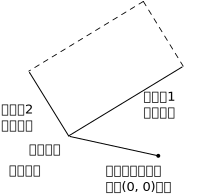
\includegraphics[width=51mm]{fig/chap2/Fig2.15a.pdf}
\begin{quote}
\heading{Figure 2.15:} A frame is described by three vectors --- an origin and two edges.
\end{quote}
\end{figure}

\noindent
We will use coordinates in the unit square \( (0 \le x, y \le 1) \) to specify
images.  With each frame, we associate a \newterm{frame coordinate map}, which
will be used to shift and scale images to fit the frame.  The map transforms
the unit square into the frame by mapping the vector \( {\bf v} = (x, y) \) to
the vector sum

私達は単位正方形\( (0 \le x, y \le 1) \)内の座標をイメージを指定するのに用いることにします。
各フレームは、フレームに適合するようにイメージの移動と拡大縮小をするのに使われる
\newterm{frame coordinate map}(フレーム座標マップ)に関連付けられます。
マップは単位正方形をベクトル\( {\bf v} = (x, y) \)を次のベクトルの和にマッピングすることで
変換します。
\begin{comment}

\begin{example}
Origin(Frame) + x * Edge_1(Frame) + y * Edge_2(Frame)
\end{example}

\end{comment}
\begin{displaymath}
 {\rm Origin(Frame)} + x \cdot {\rm Edge_1(Frame)} + y \cdot {\rm Edge_2(Frame)}. 
\end{displaymath}
\noindent
For example, (0, 0) is mapped to the origin of the frame, (1, 1) to the vertex
diagonally opposite the origin, and (0.5, 0.5) to the center of the frame.  We
can create a frame's coordinate map with the following
procedure:\footnote{\code{Frame\-/coord\-/map} uses the vector operations described
in \link{Exercise 2.46} below, which we assume have been implemented using some
representation for vectors.  Because of data abstraction, it doesn't matter
what this vector representation is, so long as the vector operations behave
correctly.}

例えば、(0, 0)はフレームの始点に、(1, 1)は対角線上に始点の反対の頂点へ、そして
(0.5, 0.5)はフレームの中心点にマッピングされます。フレーム座標マップは以下の手続により
作成できます。\footnote{\code{frame\-/coord\-/map}はこの先の\link{Exercise 2.46}にて説明される
ベクトル操作を用います。ここでは何らかのベクトルの表現を用いて実装済みと仮定します。
データ抽象化のおかげでこのベクトルの表現がどんなものかは、ベクトル操作が正しく振る舞われる
限りにおいて問題にはなりません。}

\begin{scheme}
(define (frame-coord-map frame)
  (lambda (v)
    (add-vect
     (origin-frame frame)
     (add-vect (scale-vect (xcor-vect v)
                           (edge1-frame frame))
               (scale-vect (ycor-vect v)
                           (edge2-frame frame))))))
\end{scheme}

\noindent
Observe that applying \code{frame\-/coord\-/map} to a frame returns a procedure
that, given a vector, returns a vector.  If the argument vector is in the unit
square, the result vector will be in the frame.  For example,

\code{frame\-/coord\-/map}をフレームに適用すると、ベクトルを取りベクトルを返す手続を返すことに
注意して下さい。もし引数ベクトルが単位正方形の中なら、結果のベクトルはフレームの範囲内に
なります。例として、

\begin{scheme}
((frame-coord-map a-frame) (make-vect 0 0))
\end{scheme}

\noindent
returns the same vector as

は以下のベクトルと同じものを返します。

\begin{scheme}
(origin-frame a-frame)
\end{scheme}

\begin{quote}
\heading{\phantomsection\label{Exercise 2.46}Exercise 2.46:} A two-dimensional vector \( \bf v \)
running from the origin to a point can be represented as a pair consisting of
an \( x \)-coordinate and a \( y \)-coordinate.  Implement a data abstraction for
vectors by giving a constructor \code{make\-/vect} and corresponding selectors
\code{xcor\-/vect} and \code{ycor\-/vect}.  In terms of your selectors and
constructor, implement procedures \code{add\-/vect}, \code{sub\-/vect}, and
\code{scale\-/vect} that perform the operations vector addition, vector
subtraction, and multiplying a vector by a scalar:

始点からある点へと走る2次元ベクトル\( \bf v \)は\( x \)-座標と\( y \)-座標から成る
ペアにより表現できる。ベクトルに対するデータ抽象をコンストラクタ\code{make\-/vect}と関連する
セレクタ\code{xcor\-/vect}と\code{ycor\-/vect}を与えることにより実装せよ。
セレクタとコンストラクタを用いてベクトルの足し算、引き算、スカラによる乗算を求める操作を実行する
手続 \code{add\-/vect}, \code{sub\-/vect}, \code{scale\-/vect}を実装せよ。
\begin{comment}

\begin{example}
(x_1, y_1) + (x_2, y_2) = (x_1 + x_2, y_1 + y_2)
(x_1, y_1) - (x_2, y_2) = (x_1 - x_2, y_1 - y_2)
             s * (x, y) = (sx, sy)
\end{example}

\end{comment}
\begin{displaymath}
%  
% \eqalign{
% 	(x_1, y_1) + (x_2, y_2) 	&= (x_1 + x_2, y_1 + y_2), \cr
% 	(x_1, y_1) - (x_2, y_2) 	&= (x_1 - x_2, y_1 - y_2), \cr
% 	s \cdot (x, y) 			&= (sx, sy). \cr }
% 
\begin{array}{r@{{}={}}l}
	(x_1, y_1) + (x_2, y_2) 	& (x_1 + x_2, y_1 + y_2), \\
	(x_1, y_1) - (x_2, y_2) 	& (x_1 - x_2, y_1 - y_2), \\
	s \cdot (x, y) 			& (sx, sy). 
\end{array}
\end{displaymath}
\end{quote}

\begin{quote}
\heading{\phantomsection\label{Exercise 2.47}Exercise 2.47:} Here are two possible
constructors for frames:

ここに2つの有り得そうなフレームのコンストラクタがある

\begin{scheme}
(define (make-frame origin edge1 edge2)
  (list origin edge1 edge2))
(define (make-frame origin edge1 edge2)
  (cons origin (cons edge1 edge2)))
\end{scheme}

For each constructor supply the appropriate selectors to produce an
implementation for frames.
\end{quote}

各コンストラクタに適切な、フレームに対応する実装を生成するセレクタを提供せよ。

\subsubsection*{Painters}

A painter is represented as a procedure that, given a frame as argument, draws
a particular image shifted and scaled to fit the frame.  That is to say, if
\code{p} is a painter and \code{f} is a frame, then we produce \code{p}'s image
in \code{f} by calling \code{p} with \code{f} as argument.

ペインタはフレームを引数として与えられ特定のイメージをフレームにはまるように移動、拡大縮小
して描く手続として表現される。すなわちもし\code{p}がペインタで\code{f}がフレームである場合、
\code{f}を引数として\code{p}を呼び出すことで\code{f}の中に\code{p}のイメージを生成する。

The details of how primitive painters are implemented depend on the particular
characteristics of the graphics system and the type of image to be drawn.  For
instance, suppose we have a procedure \code{draw\-/line} that draws a line on the
screen between two specified points.  Then we can create painters for line
drawings, such as the \code{wave} painter in \link{Figure 2.10}, from lists of
line segments as follows:\footnote{\code{Segments\-/>painter} uses the
representation for line segments described in \link{Exercise 2.48} below.  It
also uses the \code{for\-/each} procedure described in \link{Exercise 2.23}.}

プリミティブなペインタがどのように実装されているかの詳細は特定のグラフィックシステムの
特質と描画されるイメージのタイプに依存します。例えばスクリーン上の2つの指定された点の間に
線を引く手続\code{draw\-/line}があると想定します。すると線分のリストから線を引くためのペインタ、
例えば\link{Figure 2.10}の\code{wave}ペインタのようなものを以下のように作ることができます。\footnote{
\code{Segments\-/>painter}は線分の表現に下記の\link{Exercise 2.48}で説明されたものを使っています。
また\link{Exercise 2.23}で説明された\code{for\-/each}を使っています。}

\begin{scheme}
(define (segments->painter segment-list)
  (lambda (frame)
    (for-each
     (lambda (segment)
       (draw-line
        ((frame-coord-map frame) 
         (start-segment segment))
        ((frame-coord-map frame)
         (end-segment segment))))
     segment-list)))
\end{scheme}

\noindent
The segments are given using coordinates with respect to the unit square.  For
each segment in the list, the painter transforms the segment endpoints with the
frame coordinate map and draws a line between the transformed points.

線分は単位正方形に対しての座標を用いて与えられます。リスト中の各線分に対して
ペインタは線分の終端をフレーム座標マップを用いて変換し、変換後の点の間に線を引きます。

Representing painters as procedures erects a powerful abstraction barrier in
the picture language.  We can create and intermix all sorts of primitive
painters, based on a variety of graphics capabilities. The details of their
implementation do not matter.  Any procedure can serve as a painter, provided
that it takes a frame as argument and draws something scaled to fit the
frame.\footnote{For example, the \code{rogers} painter of \link{Figure 2.11} was
constructed from a gray-level image.  For each point in a given frame, the
\code{rogers} painter determines the point in the image that is mapped to it
under the frame coordinate map, and shades it accordingly.  By allowing
different types of painters, we are capitalizing on the abstract data idea
discussed in \link{Section 2.1.3}, where we argued that a rational-number
representation could be anything at all that satisfies an appropriate
condition.  Here we're using the fact that a painter can be implemented in any
way at all, so long as it draws something in the designated frame.  
\link{Section 2.1.3} also showed how pairs could be implemented as procedures.  Painters
are our second example of a procedural representation for data.}

手続としてペインタを表現することは強力な抽象化バリアをピクチャーランゲージの中に
確立します。私達は全ての種類のプリミティブなペインタを種々のグラフィック機能の基盤の
上に作り、混ぜることができます。それらの実装の詳細は問題ではありません。
フレームを引数として取りフレームに適切なサイズにスケールして何かを描く
任意の手続がペインタの役を演じることができます。\footnote{
例えば\link{Figure 2.11}の\code{rogers}ペインタはグレーレベルのイメージから構築されています。
与えられたフレームの中の各点に対し\code{rogers}ペインタはイメージ中のマッピングされる位置を
フレーム座標マップの下に決定し、適切に影を付けます。異なるタイプのペインタを許可することで、
\link{Section 2.1.3}で議論された分数表現は適切な条件を満たせば全く任意でかまわないという抽象データの
考えからより大きな利点を得ています。ここではペインタは指定されたフレーム内に何かを描くので
あれば全くどのように実装されても構わないという事実を用いています。\link{Section 2.1.3}はまた
ペアがどのように手続として実装され得るかということも示しました。
ペインタはデータに対する手続表現の二つ目の例です。}

\begin{quote}
\heading{\phantomsection\label{Exercise 2.48}Exercise 2.48:} A directed line segment in the
plane can be represented as a pair of vectors---the vector running from the
origin to the start-point of the segment, and the vector running from the
origin to the end-point of the segment.  Use your vector representation from
\link{Exercise 2.46} to define a representation for segments with a constructor
\code{make\-/segment} and selectors \code{start\-/segment} and \code{end\-/segment}.

平面上で方向を持つ線分はベクトルのペア---原点から
線分の始点へと向かうベクトルと原点から線分の終点へと向かうベクトルとして
表現可能だ。\link{Exercise 2.46}のベクトル表現を用いて、コンストラクタ\code{make\-/segment}と
セレクタ\code{start\-/segment}と\code{end\-/segment}を持つ線分表現を定義せよ。
\end{quote}

\begin{quote}
\heading{\phantomsection\label{Exercise 2.49}Exercise 2.49:} Use \code{segments\-/>painter}
to define the following primitive painters:

\code{segments\-/>painter}を用いて以下のプリミティブなペインタを定義せよ。

\begin{enumerate}[a]

\item
The painter that draws the outline of the designated frame.

指定したフレームの外枠を描くペインタ

\item
The painter that draws an ``X'' by connecting opposite corners of the frame.

フレームの反対の角を繋いで``X''を描くペインタ

\item
The painter that draws a diamond shape by connecting the midpoints of the sides
of the frame.

フレームの辺の中点を結んでダイヤモンドの形を描くペインタ

\item
The \code{wave} painter.

\code{wave}ペインタ

\end{enumerate}
\end{quote}

\subsubsection*{Transforming and combining painters}

An operation on painters (such as \code{flip\-/vert} or \code{beside}) works by
creating a painter that invokes the original painters with respect to frames
derived from the argument frame.  Thus, for example, \code{flip\-/vert} doesn't
have to know how a painter works in order to flip it---it just has to know how
to turn a frame upside down: The flipped painter just uses the original
painter, but in the inverted frame.

ペインタに対する操作(例えば\code{flip\-/vert}や\code{beside})はフレーム引数に由来する
フレームに対して元のペインタを実行するペインタを作成することで働いています。
従って例えば\code{flip\-/vert}は引っくり返す場合にもそれがどのように描かれるのかは
知る必要がありません---ただフレームをどのように引っくり返すのか知る必要がある
のみです。逆転したペインタはただ元のペインタを用いますが、フレームは逆転されて
いるのです。


Painter operations are based on the procedure \code{transform\-/painter}, which
takes as arguments a painter and information on how to transform a frame and
produces a new painter.  The transformed painter, when called on a frame,
transforms the frame and calls the original painter on the transformed frame.
The arguments to \code{transform\-/painter} are points (represented as vectors)
that specify the corners of the new frame: When mapped into the frame, the
first point specifies the new frame's origin and the other two specify the ends
of its edge vectors.  Thus, arguments within the unit square specify a frame
contained within the original frame.

ペインタ操作は\code{transform\-/painter}手続を基にしており、それはペインタとどのように
フレームを変換するかの情報を引数に取り、新しいペインタを生成します。変換されたペインタは
フレーム上にて呼ばれた時に、フレームを変換して基のペインタを変換済みのフレーム上で
呼び出します。\code{transform\-/painter}に対する引数は新しいフレームの角を指定する
(ベクトルとして表現される)複数の点です。フレームにマッピングされる時、最初の点は
新しいフレームの始点を指定し、他の2つのは辺ベクトルの終点を指定します。従って、
単位正方形内の引数は元のフレームの中に含まれるフレームを指定します。

\begin{scheme}
(define (transform-painter painter origin corner1 corner2)
  (lambda (frame)
    (let ((m (frame-coord-map frame)))
      (let ((new-origin (m origin)))
        (painter (make-frame 
                  new-origin
                  (sub-vect (m corner1) new-origin)
                  (sub-vect (m corner2) new-origin)))))))
\end{scheme}

\noindent
Here's how to flip painter images vertically:

次はどのようにペインタのイメージを縦方向に逆向きにするかです。

\begin{scheme}
(define (flip-vert painter)
  (transform-painter painter
                     (make-vect 0.0 1.0)   ~\textrm{; new \code{origin}}~
                     (make-vect 1.0 1.0)   ~\textrm{; new end of \code{edge1}}~
                     (make-vect 0.0 0.0))) ~\textrm{; new end of \code{edge2}}~
\end{scheme}

\noindent
Using \code{transform\-/painter}, we can easily define new transformations.
For example, we can define a painter that shrinks its image to the
upper-right quarter of the frame it is given:

\code{transform\-/painter}を用いることで簡単に新しい変換を定義することができます。
右上4分の1のフレームは次のようにして与えられます。

\begin{scheme}
(define (shrink-to-upper-right painter)
  (transform-painter
   painter (make-vect 0.5 0.5)
   (make-vect 1.0 0.5) (make-vect 0.5 1.0)))
\end{scheme}

\noindent
Other transformations rotate images counterclockwise by 90
degrees\footnote{\code{Rotate90} is a pure rotation only for square frames,
because it also stretches and shrinks the image to fit into the rotated frame.}

他の変換はイメージを時計回りの逆に90度回転したり、\footnote{\code{rotate90}は
四角形のフレームに対してのみの純粋な回転です。イメージもまた拡大縮小して
回転したフレームに合わせられるためです。}

\begin{scheme}
(define (rotate90 painter)
  (transform-painter painter 
                     (make-vect 1.0 0.0)
                     (make-vect 1.0 1.0)
                     (make-vect 0.0 0.0)))
\end{scheme}

\noindent
or squash images towards the center of the frame:\footnote{The diamond-shaped
images in \link{Figure 2.10} and \link{Figure 2.11} were created with
\code{squash\-/inwards} applied to \code{wave} and \code{rogers}.}

イメージをフレームの中心に向けて潰したりします。\footnote{\link{Figure 2.10}と
\link{Figure 2.11}内のひし形のイメージは\code{squash\-/inwards}を
\code{wave}と\code{rogers}に適用することで作成されました。}

\begin{scheme}
(define (squash-inwards painter)
  (transform-painter painter
                     (make-vect 0.0 0.0)
                     (make-vect 0.65 0.35)
                     (make-vect 0.35 0.65)))
\end{scheme}

\noindent
Frame transformation is also the key to defining means of combining two or more
painters.  The \code{beside} procedure, for example, takes two painters,
transforms them to paint in the left and right halves of an argument frame
respectively, and produces a new, compound painter.  When the compound painter
is given a frame, it calls the first transformed painter to paint in the left
half of the frame and calls the second transformed painter to paint in the
right half of the frame:

フレーム変換は2つ以上のペインタを接続する手段を定義するための鍵でもあります。
例えば\code{beside}手続は2つのペインタを取りそれらを引数のフレームの左半分と右半分に
それぞれ描画するように変換する新しい複合ペインタを生成します。複合ペインタがフレームを
与えられ時、1つ目の変換済みペインタを呼びフレームの左半分に描き、次に二つ目の変換済み
ペインタを呼びフレームの右半分を描きます。

\begin{scheme}
(define (beside painter1 painter2)
  (let ((split-point (make-vect 0.5 0.0)))
    (let ((paint-left
           (transform-painter 
            painter1
            (make-vect 0.0 0.0)
            split-point
            (make-vect 0.0 1.0)))
          (paint-right
           (transform-painter
            painter2
            split-point
            (make-vect 1.0 0.0)
            (make-vect 0.5 1.0))))
      (lambda (frame)
        (paint-left frame)
        (paint-right frame)))))
\end{scheme}

\noindent
Observe how the painter data abstraction, and in particular the representation
of painters as procedures, makes \code{beside} easy to implement.  The
\code{beside} procedure need not know anything about the details of the
component painters other than that each painter will draw something in its
designated frame.

ペインタのデータ抽象化と、特にペインタの手続としての表現がどのように\code{beside}の
実装を簡単にしているのか注目して下さい。\code{beside}手続はコンポーネントのペイントの
詳細について各ペインタが指定されたフレームに何かを描くこと以外は一切知る必要がありません。

\begin{quote}
\heading{\phantomsection\label{Exercise 2.50}Exercise 2.50:} Define the transformation
\code{flip\-/horiz}, which flips painters horizontally, and transformations that
rotate painters counterclockwise by 180 degrees and 270 degrees.

ペインタを水平方向に引っくり返す変換\code{flip\-/horiz}を定義せよ。
またペインタを時計と逆回りに180度と270度回す変換を定義せよ。
\end{quote}

\begin{quote}
\heading{\phantomsection\label{Exercise 2.51}Exercise 2.51:} Define the \code{below} operation
for painters.  \code{Below} takes two painters as arguments.  The resulting
painter, given a frame, draws with the first painter in the bottom of the frame
and with the second painter in the top.  Define \code{below} in two different
ways---first by writing a procedure that is analogous to the \code{beside}
procedure given above, and again in terms of \code{beside} and suitable
rotation operations (from \link{Exercise 2.50}).

ペインタに対する\code{below}命令を定義せよ。\code{below}は2つのペインタを引数に取る。
結果のペインタはフレームを与えられ、1つ目のペインタにてフレームの底部を描き、
2つ目のペインタにて上部を描く。\code{below}を2つの異なる方法で定義せよ。
1つは上で与えた\code{beside}と同様な方法で、2つ目は\code{beside}と適切な(\link{Exercise 2.50}の)
回転命令を利用せよ。
\end{quote}

\subsubsection*{Levels of language for robust design}

The picture language exercises some of the critical ideas we've introduced
about abstraction with procedures and data.  The fundamental data abstractions,
painters, are implemented using procedural representations, which enables the
language to handle different basic drawing capabilities in a uniform way.  The
means of combination satisfy the closure property, which permits us to easily
build up complex designs.  Finally, all the tools for abstracting procedures
are available to us for abstracting means of combination for painters.

ピクチャー言語は私達が紹介した手続とデータにようる抽象化についての重要なアイデアの
いくつかを訓練しました。基本的なデータ抽象化であるペインタは手続表現を用いて実装され
言語に異なる基礎的な描画能力を統一した方法で扱うことを可能にしました。
接続手段は閉包の性質を満たし簡単に複雑な設計を組み上げることを可能にしました。
最後に、抽象化手続に対する全てのツールはペインタに対する接続手段の抽象化にとって
有効でした。

We have also obtained a glimpse of another crucial idea about languages and
program design.  This is the approach of \newterm{stratified design}, the
notion that a complex system should be structured as a sequence of levels that
are described using a sequence of languages.  Each level is constructed by
combining parts that are regarded as primitive at that level, and the parts
constructed at each level are used as primitives at the next level.  The
language used at each level of a stratified design has primitives, means of
combination, and means of abstraction appropriate to that level of detail.

私達はまた言語とプログラム設計に関する素晴しい考えを垣間見ることができました。
これは\newterm{stratified design}(階層化設計)の方法で、複雑なシステムは一連の
言語を用いて記述される一連のレベルとして構造化されるべきであるという概念です。
各レベルはパーツをパーツを接続して構築され、それらは次のレベルではプリミティブとして
参照されます。そして各レベルで構築されたパーツは次のレベルにてプリミティブとして
使用されます。階層化された設計の各レベルで使用される言語はプリミティブ、
接続手段、そしてそのレベルの詳細さに適切な抽象化手段を持っています。

Stratified design pervades the engineering of complex systems.  For example, in
computer engineering, resistors and transistors are combined (and described
using a language of analog circuits) to produce parts such as and-gates and
or-gates, which form the primitives of a language for digital-circuit
design.\footnote{\link{Section 3.3.4} describes one such language.} These parts
are combined to build processors, bus structures, and memory systems, which are
in turn combined to form computers, using languages appropriate to computer
architecture.  Computers are combined to form distributed systems, using
languages appropriate for describing network interconnections, and so on.

階層化された設計は複雑なシステムの設計において普及しています。例えば
計算機設計では抵抗とトランジスタは接続され(そしてアナログ回路
言語を用いて記述され)ANDゲートやORゲートのようなパーツを生じ、それらがデジタル回路
の言語のプリミティブを形成します。\footnote{\link{Section 3.3.4}がそのような言語について
記述します。} このようなパーツはプロセッサ、バス構造、メモリシステムを構築するために
接続され、それらはコンピュータを形成するために接続され、コンピュータアーキテクチャに
相応しい言語を用います。コンピュータは分散システムを形成するために接続され、
ネットワーク相互接続その他を記述するに適切な言語を用います。

As a tiny example of stratification, our picture language uses primitive
elements (primitive painters) that are created using a language that specifies
points and lines to provide the lists of line segments for
\code{segments\-/>painter}, or the shading details for a painter like
\code{rogers}.  The bulk of our description of the picture language focused on
combining these primitives, using geometric combiners such as \code{beside} and
\code{below}.  We also worked at a higher level, regarding \code{beside} and
\code{below} as primitives to be manipulated in a language whose operations,
such as \code{square\-/of\-/four}, capture common patterns of combining geometric
combiners.

階層化の簡単な例として、ピクチャー言語はプリミティブな要素(プリミティブペインタ)を
用い、それらは点と線を指定し\code{segments\-/>painter}のための線分のリストを提供したり、
\code{rogers}のようなペインタに対するシェーディングの詳細を提供したりする言語を
用いて作成されました。私達のピクチャー言語の説明の大部分がこれらのプリミティブを接続し
\code{beside}や\code{below}のような幾何学的なコンバイナ(結合器)に充てられました。
私達はまたより高階なレベルにおいて\code{beside}と\code{below}をプリミティブとして見做し
\code{square\-/of\-/four}のような命令を持つ言語において幾何学的結合器を接続する共通の
パターンを獲得することに努めました。

Stratified design helps make programs \newterm{robust}, that is, it makes it
likely that small changes in a specification will require correspondingly small
changes in the program.  For instance, suppose we wanted to change the image
based on \code{wave} shown in \link{Figure 2.9}.  We could work at the lowest
level to change the detailed appearance of the \code{wave} element; we could
work at the middle level to change the way \code{corner\-/split} replicates the
\code{wave}; we could work at the highest level to change how
\code{square\-/limit} arranges the four copies of the corner.  In general, each
level of a stratified design provides a different vocabulary for expressing the
characteristics of the system, and a different kind of ability to change it.

階層化設計はプログラムを\newterm{robust}(堅牢)にすることを手助けします。
それはつまりプログラムにおける仕様上の小さな変更が相応した小さな変更を
要求することを意味します。例えば\link{Figure 2.9}で示された\code{wave}のイメージ
を変更したいとします。\code{wave}要素の詳細な表現を変更する最も低レベルで行うことも
可能ですが、中間のレベルにおいて\code{corner\-/split}が\code{wave}をどのように複製するか
について行うことも可能ですし、最高レベルにおいて\code{square\-/limit}がどのように角の
4つのコピーを配置するかについて変更することも可能です。一般的に階層設計の各レベル
は異なる語彙をシステムの特徴を表すのに提供します。そして異なる種類の変更方法をも
提供します。

\begin{quote}
\heading{\phantomsection\label{Exercise 2.52}Exercise 2.52:} Make changes to the square limit
of \code{wave} shown in \link{Figure 2.9} by working at each of the levels
described above.  In particular:

\link{Figure 2.9}の\code{wave}のsquare-limitに、上で説明された各レベルで働くことで
変更を加えよ。より詳細には、

\begin{enumerate}[a]

\item
Add some segments to the primitive \code{wave} painter of \link{Exercise 2.49}
(to add a smile, for example).

\link{Exercise 2.49}のプリミティブな\code{wave}ペインタにいくつか線分を加えよ。
(例えば笑顔を追加せよ)

\item
Change the pattern constructed by \code{corner\-/split} (for example, by using
only one copy of the \code{up\-/split} and \code{right\-/split} images instead of
two).

\code{corner\-/split}により構築されるパターンを変更せよ
(例えば\code{up\-/split}や\code{right\-/split}のイメージを2つでなく1つにせよ)

\item
Modify the version of \code{square\-/limit} that uses \code{square\-/of\-/four} so as
to assemble the corners in a different pattern.  (For example, you might make
the big Mr. Rogers look outward from each corner of the square.)

\code{square\-/of\-/four}を用いる\code{square\-/limit}のバージョンを変更し角を異なるパターンで
組み立てるようにせよ。
(例えば正方形の各角にてMr. Rogersをそれぞれ外に向けよ)

\end{enumerate}
\end{quote}

\label{Section 2.3}
\section{Symbolic Data}

All the compound data objects we have used so far were constructed ultimately
from numbers.  In this section we extend the representational capability of our
language by introducing the ability to work with arbitrary symbols as data.

私達がここまで使用した全ての複合データオブジェクトは最終的には数値から構築されていました。
この節では任意のシンボル(記号)をデータとして用いる能力を紹介することで、言語の表現力を拡張します。



\label{Section 2.3.1}
\subsection{Quotation}

If we can form compound data using symbols, we can have lists such as

もし記号を用いて複合データを形成できれば以下のようなリストを持つことができます。

\begin{scheme}
(a b c d)
(23 45 17)
((Norah 12) (Molly 9) (Anna 7) (Lauren 6) (Charlotte 4))
\end{scheme}

\noindent
Lists containing symbols can look just like the expressions of our
language:

記号を含むリストは言語の式と全く同じように見えます。

\begin{scheme}
(* (+ 23 45) 
   (+ x 9))
(define (fact n) 
  (if (= n 1) 1 (* n (fact (- n 1)))))
\end{scheme}

\noindent
In order to manipulate symbols we need a new element in our language: the
ability to \newterm{quote} a data object.  Suppose we want to construct the
list \code{(a b)}.  We can't accomplish this with \code{(list a b)}, because
this expression constructs a list of the \newterm{values} of \code{a} and
\code{b} rather than the symbols themselves.  This issue is well known in the
context of natural languages, where words and sentences may be regarded either
as semantic entities or as character strings (syntactic entities).  The common
practice in natural languages is to use quotation marks to indicate that a word
or a sentence is to be treated literally as a string of characters.  For
instance, the first letter of ``John'' is clearly ``J.''  If we tell somebody
``say your name aloud,'' we expect to hear that person's name.  However, if we
tell somebody ``say `your name' aloud,'' we expect to hear the words ``your
name.''  Note that we are forced to nest quotation marks to describe what
somebody else might say.\footnote{Allowing quotation in a language wreaks havoc
with the ability to reason about the language in simple terms, because it
destroys the notion that equals can be substituted for equals.  For example,
three is one plus two, but the word ``three'' is not the phrase ``one plus
two.''  Quotation is powerful because it gives us a way to build expressions
that manipulate other expressions (as we will see when we write an interpreter
in \link{Chapter 4}). But allowing statements in a language that talk about
other statements in that language makes it very difficult to maintain any
coherent principle of what ``equals can be substituted for equals'' should
mean.  For example, if we know that the evening star is the morning star, then
from the statement ``the evening star is Venus'' we can deduce ``the morning
star is Venus.''  However, given that ``John knows that the evening star is
Venus'' we cannot infer that ``John knows that the morning star is Venus.''}

記号を扱う目的のためには言語に新しい要素を必要とします。データオブジェクトを
\newterm{quote}(引用)する能力です。例えばリスト\code{(a b)}を構築したいとします。
私達はこれを\code{(list a b)}を用いては達成できません。なぜならこの式は\code{a}と
\code{b}の値からリストを構築する式であり、記号それ自体ではないからです。
この問題は自然言語の文脈では良く知られていて、単語と文が意味上の要素として見做さ
れているか、または文字列(文法上の要素)として見做されているかの場合が有り得ます。
自然言語での共通な慣例は単語や文が文字通りに扱われることを示すためにクォーテーション
マークを用いることです。例えば``John''の最初の文字は明らかに``J''です。
もし私達が誰かに``貴方の名前を大きな声で言って''と伝えれば、その人の名前を
聞くことを期待します。しかしもし誰かに`` `貴方の名前'と大きな声で言って''と伝えれば
``貴方の名前''という語を聞くことを期待するでしょう。私達がクォーテーションマークを
入れ子にすることを第三者が何を言うだろうかを説明するために強制されていることに
注意して下さい。\footnote{言語の中でクォーテーションを許可することが簡単な語で
言語について推論する能力を与えると共に大きな破壊をもたらしています。それが
等値な物は等値な物と置換できるという概念を破壊するためです。例えば1足す2は3ですが
``3''という語は``1足す2''という語句ではありません。クォーテーションは他の表現を
操作する表現を構築する手段を提供するため強力です。(\link{Chapter 4}でインタプリタを
書く時に学びます)。しかし言語の中で、同じ言語の他の文について話す文を許すことは
``等値な物は等値な物と交換できる''が何を意味すべきかという任意の一貫性を保守すること
をとても難しくします。例えばもし私達が宵の明星が明けの明星と同じであることを知っている
場合、``宵の明星は金星''という文から``明けの明星は金星''であることを推論できます。
しかし``Johnは宵の明星が金星であることを知っている''を与えられても``Johnは明けの明星
が金星であることを知っている''とは推論することはできません。}

We can follow this same practice to identify lists and symbols that are to be
treated as data objects rather than as expressions to be evaluated.  However,
our format for quoting differs from that of natural languages in that we place
a quotation mark (traditionally, the single quote symbol \code{'}) only at the
beginning of the object to be quoted.  We can get away with this in Scheme
syntax because we rely on blanks and parentheses to delimit objects.  Thus, the
meaning of the single quote character is to quote the next object.\footnote{The
single quote is different from the double quote we have been using to enclose
character strings to be printed.  Whereas the single quote can be used to
denote lists or symbols, the double quote is used only with character strings.
In this book, the only use for character strings is as items to be printed.}

データオブジェクトとして扱われるべきであり、式として評価
されるべきではないリストとシンボルを区別するために、これと同じ習慣に従うことができます。
しかしクォートする形式は自然言語のそれとは異なり、クォーテーションマーク(伝統的に
シングルクォートの記号 \code{'})はクォートされるべきオブジェクトの先頭にのみ置かれます。
Schemeの文法でこの様に逃れられるのはオブジェクトを区切るのに空白と括弧を信頼することが
できるためです。従ってシングルクォート文字の意味は次のオブジェクトをクォートすることに
なります。\footnote{シングルクォートは表示される文字列を囲むのに使用してきたダブルクォート
とは異なります。シングルクォートがリストやシンボルを示すのに対し、ダブルクォートは
文字列と共にのみ利用されます。この本では文字列の使用方法は表示されるための項目としてのみ
です。}

Now we can distinguish between symbols and their values:

これでシンボルとその値を区別することが可能です。

\begin{scheme}
(define a 1)
(define b 2)
(list a b)
~\textit{(1 2)}~
(list 'a 'b)
~\textit{(a b)}~
(list 'a b)
~\textit{(a 2)}~
\end{scheme}

\noindent
Quotation also allows us to type in compound objects, using the conventional
printed representation for lists:\footnote{Strictly, our use of the quotation
mark violates the general rule that all compound expressions in our language
should be delimited by parentheses and look like lists.  We can recover this
consistency by introducing a special form \code{quote}, which serves the same
purpose as the quotation mark.  Thus, we would type \code{(quote a)} instead of
\code{'a}, and we would type \code{(quote (a b c))} instead of \code{'(a b c)}.
This is precisely how the interpreter works.  The quotation mark is just a
single-character abbreviation for wrapping the next complete expression with
\code{quote} to form \( \hbox{\ttfamily(quote}\;\langle\kern0.06em\hbox{\ttfamily\slshape expression}\kern0.08em\rangle\hbox{\ttfamily)} \).  This is
important because it maintains the principle that any expression seen by the
interpreter can be manipulated as a data object.  For instance, we could
construct the expression \code{(car '(a b c))}, which is the same as \code{(car
(quote (a b c)))}, by evaluating \code{(list 'car (list 'quote '(a b c)))}.}

クォーテーションはまた慣習的なリストに対する印字された表現を用いて
複合オブジェクトの入力も可能にします。\footnote{厳密には私達のクォーテーションマークの
使用方法は言語における全ての複合式は括弧で区切られリストのように見えるという
全体のルールを破ります。この整合性に対しては特殊形式\code{quote}を紹介することで
回復することが可能です。これはクォーテーションマークと同じ目的を演じます。
従って\code{'a}の代わりに\code{(quote a)}と入力できますし、\code{'(a b c)}の代わりに
\code{(quote (a b c))}と入力できます。これはインタプリタは正確にはどのように働くか
ということです。クォーテーションマークは単一文字による省略形に過ぎず次の完全な
式を\code{quote}でラッピングすることで
\( \hbox{\ttfamily(quote}\;\langle\kern0.06em\hbox{\ttfamily\slshape expression}\kern0.08em\rangle\hbox{\ttfamily)} \)
を形成します。これは重要なことです。なぜならインタプリタに読まれる任意の式がデータオブジェクト
として扱うことができるという原則を保持するからです。例えば\code{(car '(a b c))}という式は
\code{(car (quote (a b c)))}と同じで、\code{(list 'car (list 'quote '(a b c)))}
を評価することで構築できます。}

\begin{scheme}
(car '(a b c))
~\textit{a}~
(cdr '(a b c))
~\textit{(b c)}~
\end{scheme}

\noindent
In keeping with this, we can obtain the empty list by evaluating \code{'()},
and thus dispense with the variable \code{nil}.

これを守ることで、空リストを\code{'()}を評価して得ることができます。
従って、変数\code{nil}の使用を止められます。

One additional primitive used in manipulating symbols is \code{eq?}, which
takes two symbols as arguments and tests whether they are the same.\footnote{We
can consider two symbols to be ``the same'' if they consist of the same
characters in the same order.  Such a definition skirts a deep issue that we
are not yet ready to address: the meaning of ``sameness'' in a programming
language.  We will return to this in \link{Chapter 3} (\link{Section 3.1.3}).}
Using \code{eq?}, we can implement a useful procedure called \code{memq}.  This
takes two arguments, a symbol and a list.  If the symbol is not contained in
the list (i.e., is not \code{eq?} to any item in the list), then \code{memq}
returns false.  Otherwise, it returns the sublist of the list beginning with
the first occurrence of the symbol:

記号を操作するのに使われるもう1つ追加のプリミティブとして\code{eq?}があります。
これは2つのシンボルを引数として取りそれらが同じであるかテストします。\footnote{
2つのシンボルが同じ文字で同じ順に構成されている場合にそれらが``同じ''であると
考えることができます。そのような定義はまだ私達が解決するには準備の足りない深い
問題を回避しています。プログラミング言語における``同一性''の意味です。
私達はこの問題に\link{Chapter 3} (\link{Section 3.1.3})にて戻ります。}
\code{eq?}を用いることで\code{memq}と呼ばれる便利な手続を実装できます。これは2つの引数、
シンボルとリストを取ります。もしシンボルがリストに含まれていない場合(つまり
リスト中のどの項目にも\code{eq?}でない場合)\code{memq}はfalseを返します。そうでなければ
リスト中のそのシンボルが最初に出現する場所からのサブリストを返します。

\begin{scheme}
(define (memq item x)
  (cond ((null? x) false)
        ((eq? item (car x)) x)
        (else (memq item (cdr x)))))
\end{scheme}

\noindent
For example, the value of
例えば、次の式の値は

\begin{scheme}
(memq 'apple '(pear banana prune))
\end{scheme}

\noindent
is false, whereas the value of

falseになります。そして次の式の値は

\begin{scheme}
(memq 'apple '(x (apple sauce) y apple pear))
\end{scheme}

\noindent
is \code{(apple pear)}.

\code{(apple pear)}です。

\begin{quote}
\heading{\phantomsection\label{Exercise 2.53}Exercise 2.53:} What would the interpreter print
in response to evaluating each of the following expressions?

以下の式のそれぞれを評価した応答としてインタプリタは何を表示するか?

\begin{scheme}
(list 'a 'b 'c)
(list (list 'george))
(cdr '((x1 x2) (y1 y2)))
(cadr '((x1 x2) (y1 y2)))
(pair? (car '(a short list)))
(memq 'red '((red shoes) (blue socks)))
(memq 'red '(red shoes blue socks))
\end{scheme}
\end{quote}

\begin{quote}
\heading{\phantomsection\label{Exercise 2.54}Exercise 2.54:} Two lists are said to be
\code{equal?} if they contain equal elements arranged in the same order.  For
example,

2つのリストはそれぞれが同じ要素を同じ順で持っている場合に\code{equal?}と言える。
例えば

\begin{scheme}
(equal? '(this is a list) '(this is a list))
\end{scheme}

\noindent
is true, but

は真であるが

\begin{scheme}
(equal? '(this is a list) '(this (is a) list))
\end{scheme}

\noindent
is false.  To be more precise, we can define \code{equal?}  recursively in
terms of the basic \code{eq?} equality of symbols by saying that \code{a} and
\code{b} are \code{equal?} if they are both symbols and the symbols are
\code{eq?}, or if they are both lists such that \code{(car a)} is \code{equal?}
to \code{(car b)} and \code{(cdr a)} is \code{equal?} to \code{(cdr b)}.  Using
this idea, implement \code{equal?} as a procedure.\footnote{In practice,
programmers use \code{equal?} to compare lists that contain numbers as well as
symbols.  Numbers are not considered to be symbols.  The question of whether
two numerically equal numbers (as tested by \code{=}) are also \code{eq?} is
highly implementation-dependent.  A better definition of \code{equal?} (such as
the one that comes as a primitive in Scheme) would also stipulate that if
\code{a} and \code{b} are both numbers, then \code{a} and \code{b} are
\code{equal?} if they are numerically equal.}

は偽である。具体的には基本となる\code{eq?}の記号の等価性を再帰的に用いて\code{equal?}
を定義できる。\code{a}と\code{b}が\code{equal?}であるとはそれらが両方とも記号である場合、かつ
記号が\code{eq?}である場合、または両方ともリストであり\code{(car a)}が\code{(car b)}に
\code{equal?}であり、かつ\code{(cdr a)}が\code{(cdr b)}に\code{equal?}であるような場合である。
この考えを用いて\code{equal?}を手続として実装せよ。\footnote{
実際には、プログラマは\code{equal?}を数値と同じくシンボルを含むリストの比較に用いる。
数値は記号とは認識されない。数の上で等しい二つの数値(\code{=}でテストした場合の様に)が
\code{eq?}でもそうであるかという問題は高度に実装依存である。\code{equal?}の
(Schemeにプリミティブとして提供されているような)より良い定義でも、もし\code{a}と\code{b}が
数値であるなら、それらが数値として等しい場合に\code{equal?}であると明記するだろう。}
 
\end{quote}

\begin{quote}
\heading{\phantomsection\label{Exercise 2.55}Exercise 2.55:} Eva Lu Ator types to the
interpreter the expression

Eva Lu Atorはインタプリタに次の式を入力した。

\begin{scheme}
(car ''abracadabra)
\end{scheme}

To her surprise, the interpreter prints back \code{quote}.  Explain.

驚いたことにインタプリタは\code{quote}を応答として表示した。説明せよ。
\end{quote}

\label{Section 2.3.2}
\subsection{Example: Symbolic Differentiation}

As an illustration of symbol manipulation and a further illustration of data
abstraction, consider the design of a procedure that performs symbolic
differentiation of algebraic expressions.  We would like the procedure to take
as arguments an algebraic expression and a variable and to return the
derivative of the expression with respect to the variable.  For example, if the
arguments to the procedure are \( ax^2 + bx + c \) and \( x \), the
procedure should return \( 2ax + b \).  Symbolic differentiation is of
special historical significance in Lisp.  It was one of the motivating examples
behind the development of a computer language for symbol manipulation.
Furthermore, it marked the beginning of the line of research that led to the
development of powerful systems for symbolic mathematical work, which are
currently being used by a growing number of applied mathematicians and
physicists.

記号操作の説明として、及びより一層のデータ抽象の説明として、代数式の記号微分を
行う手続の設計について考えてみましょう。手続は引数として代数式と変数を取り
変数に対する式の導関数を返すことにします。例えば手続に対する引数が
\( ax^2 + bx + c \)と\( x \)の時、手続は\( 2ax + b \)を返さなければいけません。
記号微分はLispにとって歴史的に特別な意味があります。記号操作のためのコンピュータ言語
の開発の裏にこれがその動機の一例として存在しました。さらにこれが現在増大する応用数学者
及び科学者に用いられている記号数理の成果の
ための強力なシステムの開発へと導く一連の研究の始まりに跡を残しました。

In developing the symbolic-differentiation program, we will follow the same
strategy of data abstraction that we followed in developing the rational-number
system of \link{Section 2.1.1}.  That is, we will first define a differentiation
algorithm that operates on abstract objects such as ``sums,'' ``products,'' and
``variables'' without worrying about how these are to be represented.  Only
afterward will we address the representation problem.

記号微分プログラムの開発においても\link{Section 2.1.1}の分数システムの開発と
同じデータ抽象化の戦略に従います。最初に``sums,'' ``products,'' ``variables''
のような抽象オブジェクトを操作する微分アルゴリズムを定義します。
これらがどのように表現されているのかについて心配することありません。
後程、表現上の問題については解決しましょう。

\subsubsection*{The differentiation program with abstract data}

In order to keep things simple, we will consider a very simple
symbolic-differentiation program that handles expressions that are built up
using only the operations of addition and multiplication with two arguments.
Differentiation of any such expression can be carried out by applying the
following reduction rules:

問題を簡単にするために、二引数の足し算とかけ算の命令のみから構築される式のみを扱う
とても簡単な記号微分プログラムについて考えましょう。任意のそのような式の微分は以下の
簡約ルールを適用することで実行されます。

\begin{comment}

\begin{example}
dc
-- = 0  for c a constant, or a variable different from x
dx

dx
-- = 1
dx

d(u + v)   du   dv
-------- = -- + --
   dx      dx   dx

d(uv)     / dv \     / du \
----- = u | -- | + v | -- |
 dx       \ dx /     \ dx /
\end{example}

\end{comment}
\label{Section 2.3.2}
\subsection{Example: Symbolic Differentiation}

As an illustration of symbol manipulation and a further illustration of data
abstraction, consider the design of a procedure that performs symbolic
differentiation of algebraic expressions.  We would like the procedure to take
as arguments an algebraic expression and a variable and to return the
derivative of the expression with respect to the variable.  For example, if the
arguments to the procedure are \( ax^2 + bx + c \) and \( x \), the
procedure should return \( 2ax + b \).  Symbolic differentiation is of
special historical significance in Lisp.  It was one of the motivating examples
behind the development of a computer language for symbol manipulation.
Furthermore, it marked the beginning of the line of research that led to the
development of powerful systems for symbolic mathematical work, which are
currently being used by a growing number of applied mathematicians and
physicists.

記号操作の説明として、及びより一層のデータ抽象の説明として、代数式の記号微分を
行う手続の設計について考えてみましょう。手続は引数として代数式と変数を取り
変数に対する式の導関数を返すことにします。例えば手続に対する引数が
\( ax^2 + bx + c \)と\( x \)の時、手続は\( 2ax + b \)を返さなければいけません。
記号微分はLispにとって歴史的に特別な意味があります。記号操作のためのコンピュータ言語
の開発の裏にこれがその動機の一例として存在しました。さらにこれが現在増大する応用数学者
及び科学者に用いられている記号数理の成果の
ための強力なシステムの開発へと導く一連の研究の始まりに跡を残しました。

In developing the symbolic-differentiation program, we will follow the same
strategy of data abstraction that we followed in developing the rational-number
system of \link{Section 2.1.1}.  That is, we will first define a differentiation
algorithm that operates on abstract objects such as ``sums,'' ``products,'' and
``variables'' without worrying about how these are to be represented.  Only
afterward will we address the representation problem.

記号微分プログラムの開発においても\link{Section 2.1.1}の分数システムの開発と
同じデータ抽象化の戦略に従います。最初に``sums,'' ``products,'' ``variables''
のような抽象オブジェクトを操作する微分アルゴリズムを定義します。
これらがどのように表現されているのかについて心配することありません。
後程、表現上の問題については解決しましょう。

\subsubsection*{The differentiation program with abstract data}

In order to keep things simple, we will consider a very simple
symbolic-differentiation program that handles expressions that are built up
using only the operations of addition and multiplication with two arguments.
Differentiation of any such expression can be carried out by applying the
following reduction rules:

問題を簡単にするために、二引数の足し算とかけ算の命令のみから構築される式のみを扱う
とても簡単な記号微分プログラムについて考えましょう。任意のそのような式の微分は以下の
簡約ルールを適用することで実行されます。

\begin{comment}

\begin{example}
dc
-- = 0  for c a constant, or a variable different from x
dx

dx
-- = 1
dx

d(u + v)   du   dv
-------- = -- + --
   dx      dx   dx

d(uv)     / dv \     / du \
----- = u | -- | + v | -- |
 dx       \ dx /     \ dx /
\end{example}

\end{comment}
\begin{displaymath}
{{\it dc} \over {\it dx}} 		= 0, 
	\quad c\ \mbox{は定数か、} x\ \mbox{と異なる変数}, 
\end{displaymath}
\begin{displaymath}
{{\it dx} \over {\it dx}} 		= 1, 
\end{displaymath}
\begin{displaymath}
{{\it d\,(u + v\,)} \over {\it dx}} 	= {{\it du} \over {\it dx}} + {{\it dv} \over {\it dx}}, 
\end{displaymath}
\begin{displaymath}
{{\it d\,(uv\,)} \over {\it dx}} 	= u {{\it dv} \over {\it dx}} + v {{\it du} \over {\it dx}}. 
\end{displaymath}


\noindent
Observe that the latter two rules are recursive in nature.  That is, to obtain
the derivative of a sum we first find the derivatives of the terms and add
them.  Each of the terms may in turn be an expression that needs to be
decomposed.  Decomposing into smaller and smaller pieces will eventually
produce pieces that are either constants or variables, whose derivatives will
be either 0 or 1.

後者の2つのルールは自然に再帰的であることに注意して下さい。つまり和の導関数を得る
ためには最初に項の導関数を求めそれらを足す必要があります。各項は順に分解が必要な
式に成り得ます。順により小さな部分へと分解していくことはやがて定数か、その導関数が
0か1のどちらかになる変数になります。

To embody these rules in a procedure we indulge in a little wishful thinking,
as we did in designing the rational-number implementation.  If we had a means
for representing algebraic expressions, we should be able to tell whether an
expression is a sum, a product, a constant, or a variable.  We should be able
to extract the parts of an expression.  For a sum, for example we want to be
able to extract the addend (first term) and the augend (second term).  We
should also be able to construct expressions from parts.  Let us assume that we
already have procedures to implement the following selectors, constructors, and
predicates:

これらのルールを手続で具体化するために、分数実装の設計で行ったように少し希望的観測
に耽ります。もし代数式を表現するための手段があるのなら式が和か積か定数であるかを
判別することができるはずです。式のパーツを抽出することができるはずです。例えば
足し算に対して加数(第一項)と被加数(第二項)を抽出できるはずです。またパーツから式を
構築することもできるはずです。既に以下のセレクタ、コンストラクタ、述語を実装するための
手続を持っていると仮定しましょう。

\begin{scheme}
(variable? e)            ~\textrm{\code{e}は変数であるか?}~
(same-variable? v1 v2)   ~\textrm{\code{v1}と\code{v2}は同じ変数であるか?}~
(sum? e)                 ~\textrm{\code{e}は和か?}~
(addend e)               ~\textrm{和\code{e}の加数.}~
(augend e)               ~\textrm{和\code{e}の被加数.}~
(make-sum a1 a2)         ~\textrm{\code{a1}と\code{a2}の和を構築する}~
(product? e)             ~\textrm{\code{e}は積か?}~
(multiplier e)           ~\textrm{積\code{e}の乗数}~
(multiplicand e)         ~\textrm{積\code{e}の被乗数}~
(make-product m1 m2)     ~\textrm{\code{m1}と\code{m2}の積を構築する}~
\end{scheme}

\noindent
Using these, and the primitive predicate \code{number?}, which identifies
numbers, we can express the differentiation rules as the following procedure:

これらと数値であるかを判断するプリミティブな述語\code{number?}を用いて、以下の手続の
様に微分のルールを表現できます。

\begin{scheme}
(define (deriv exp var)
  (cond ((number? exp) 0)
        ((variable? exp) (if (same-variable? exp var) 1 0))
        ((sum? exp) (make-sum (deriv (addend exp) var)
                              (deriv (augend exp) var)))
        ((product? exp)
         (make-sum
           (make-product (multiplier exp)
                         (deriv (multiplicand exp) var))
           (make-product (deriv (multiplier exp) var)
                         (multiplicand exp))))
        (else
         (error "unknown expression type: DERIV" exp))))
\end{scheme}

\noindent
This \code{deriv} procedure incorporates the complete differentiation
algorithm.  Since it is expressed in terms of abstract data, it will work no
matter how we choose to represent algebraic expressions, as long as we design a
proper set of selectors and constructors.  This is the issue we must address
next.

この\code{deriv}手続は完全な微分アルゴリズムに立脚しています。代数データの項により
表現されているため、適切なセレクタとコンストラクタを設計する限りにおいて、どのように
代数式を表現しても動きます。この条件の部分が次に解決すべき問題です。

\subsubsection*{Representing algebraic expressions}

We can imagine many ways to use list structure to represent algebraic
expressions.  For example, we could use lists of symbols that mirror the usual
algebraic notation, representing \( ax + b \) as the list \code{(a * x +
b)} .  However, one especially straightforward choice is to use the same
parenthesized prefix notation that Lisp uses for combinations; that is, to
represent \( ax + b \) as \code{(+ (* a x) b)}.  Then our data
representation for the differentiation problem is as follows:

代数式を表現するリスト構造を使用する手法は数多く想像できます。例えば通常の代数
記法を真似する記号のリストを用い、\( ax + b \)をリスト\code{(a * x + b)}の様に
表現することもできるでしょう。しかし特に直接的な1つの選択はLispが複合式に用いる
のと同じく括弧で括った接頭辞記述法です。つまり\( ax + b \)は\code{(+ (* a x) b)}と
表現されます。従って微分問題に対するデータ表現は以下のとおりです。

\begin{itemize}

\item
The variables are symbols.  They are identified by the primitive predicate
\code{symbol?}:

変数はシンボルである。プリミティブな述語\code{symbol?}で判別される。

\begin{scheme}
(define (variable? x) (symbol? x))
\end{scheme}

\item
Two variables are the same if the symbols representing them are \code{eq?}:

2つの変数はそれらを表現するシンボルが\code{eq?}である時同じだ。

\begin{scheme}
(define (same-variable? v1 v2)
  (and (variable? v1) (variable? v2) (eq? v1 v2)))
\end{scheme}

\item
Sums and products are constructed as lists:

和と積はリストとして構築される。

\begin{scheme}
(define (make-sum a1 a2) (list '+ a1 a2))
(define (make-product m1 m2) (list '* m1 m2))
\end{scheme}

\item
A sum is a list whose first element is the symbol \code{+}:

和は最初の要素がシンボル\code{+}のリストだ。

\begin{scheme}
(define (sum? x) (and (pair? x) (eq? (car x) '+)))
\end{scheme}

\item
The addend is the second item of the sum list:

加数は和のリストの二つ目の項だ。

\begin{scheme}
(define (addend s) (cadr s))
\end{scheme}

\item
The augend is the third item of the sum list:

被加数は和のリストの三つめの項だ。

\begin{scheme}
(define (augend s) (caddr s))
\end{scheme}

\item
A product is a list whose first element is the symbol \code{*}:

積は最初の要素がシンボル\code{*}のリストだ。

\begin{scheme}
(define (product? x) (and (pair? x) (eq? (car x) '*)))
\end{scheme}

\item
The multiplier is the second item of the product list:

乗数は積のリストの二つ目の項だ。

\begin{scheme}
(define (multiplier p) (cadr p))
\end{scheme}

\item
The multiplicand is the third item of the product list:

被乗数は積のリストの三つめの項だ。

\begin{scheme}
(define (multiplicand p) (caddr p))
\end{scheme}

\end{itemize}

\noindent
Thus, we need only combine these with the algorithm as embodied by \code{deriv}
in order to have a working symbolic-differentiation program.  Let us look at
some examples of its behavior:

従って記号微分プログラムを得るためには、これらを\code{deriv}により組込まれた
アルゴリズムを用いて組み立てることのみが必要でです。いくつかの例とその振舞を
見てみましょう。

\begin{scheme}
(deriv '(+ x 3) 'x)
~\textit{(+ 1 0)}~
(deriv '(* x y) 'x)
~\textit{(+ (* x 0) (* 1 y))}~
(deriv '(* (* x y) (+ x 3)) 'x)
~\textit{(+ (* (* x y) (+ 1 0))}~
   ~\textit{(* (+ (* x 0) (* 1 y))}~
      ~\textit{(+  x 3)))}~
\end{scheme}

\noindent
The program produces answers that are correct; however, they are unsimplified.
It is true that

プログラムは正しい解答を生成します。しかし、それらは簡略化されていません。
\begin{comment}

\begin{example}
d(xy)
----- = x * 0 + 1 * y
 dx
\end{example}

\end{comment}
\begin{displaymath}
 {{\it d\,(xy)} \over {\it dx}} = x \cdot 0 + 1 \cdot y, 
\end{displaymath}
\noindent
but we would like the program to know that \( x \cdot 0 = 0 \), \( 1 \cdot y = y \),
and \( 0 + y = y \).  The answer for the second example should have been
simply \code{y}.  As the third example shows, this becomes a serious issue when
the expressions are complex.

しかし私達はこのプログラムに\( x \cdot 0 = 0 \), \( 1 \cdot y = y \),
\( 0 + y = y \)を理解して欲しいと望みます。二つ目の例の解答は単純に\code{y}となるべき
です。三つめの例が示すように、これは式が複雑な場合には深刻な問題となります。

Our difficulty is much like the one we encountered with the rational-number
implementation: we haven't reduced answers to simplest form.  To accomplish the
rational-number reduction, we needed to change only the constructors and the
selectors of the implementation.  We can adopt a similar strategy here.  We
won't change \code{deriv} at all.  Instead, we will change \code{make\-/sum} so
that if both summands are numbers, \code{make\-/sum} will add them and return
their sum.  Also, if one of the summands is 0, then \code{make\-/sum} will return
the other summand.

この困難は分数実装において出くわしたものととても似ています。最も単純な形式に解答を
約分していませんでした。分数を約分するためには実装のコンストラクタとセレクタのみを
変更する必要がありました。ここでも同様の戦略を受け入れることができます。\code{deriv}には
全く変更は加えません。その代わりに\code{make\-/sum}を変更し両方の加数が数値である場合、
\code{make\-/sum}はそれらを足してその和を返します。また加数の1つが0ならば\code{make\-/sum}は
もう一方の加数を返します。

\begin{scheme}
(define (make-sum a1 a2)
  (cond ((=number? a1 0) a2)
        ((=number? a2 0) a1)
        ((and (number? a1) (number? a2))
         (+ a1 a2))
        (else (list '+ a1 a2))))
\end{scheme}

\noindent
This uses the procedure \code{=number?}, which checks whether an expression is
equal to a given number:

これには手続\code{=number?}を用いました。式が与えられた数値と等しいかチェックします。

\begin{scheme}
(define (=number? exp num) (and (number? exp) (= exp num)))
\end{scheme}

\noindent
Similarly, we will change \code{make\-/product} to build in the rules that 0
times anything is 0 and 1 times anything is the thing itself:

同様に\code{make\-/product}を変更し任意の項に0を掛ければ0、任意の項に1を掛ければそれ自身に
するルールを構築します。


\begin{scheme}
(define (make-product m1 m2)
  (cond ((or (=number? m1 0) (=number? m2 0)) 0)
        ((=number? m1 1) m2)
        ((=number? m2 1) m1)
        ((and (number? m1) (number? m2)) (* m1 m2))
        (else (list '* m1 m2))))
\end{scheme}

\noindent
Here is how this version works on our three examples:

これがこのバージョンが先程の3つの例でどのように動くかです

\begin{scheme}
(deriv '(+ x 3) 'x)
~\textit{1}~
(deriv '(* x y) 'x)
~\textit{y}~
(deriv '(* (* x y) (+ x 3)) 'x)
~\textit{(+ (* x y) (* y (+ x 3)))}~
\end{scheme}

\noindent
Although this is quite an improvement, the third example shows that there is
still a long way to go before we get a program that puts expressions into a
form that we might agree is ``simplest.''  The problem of algebraic
simplification is complex because, among other reasons, a form that may be
simplest for one purpose may not be for another.

これはとても改善が見られますが、三つめの例は
式を``最も単純''だと同意を得られる形式に変形するプログラムを得るまでには
今だ長い道程があることを示します。代数の簡約の問題は複雑です。他の理由の中でも、
ある目的にとって最も単純な形式が他の目的にとってはそうではないことが有り得る
ためです。

\begin{quote}
\heading{\phantomsection\label{Exercise 2.56}Exercise 2.56:} Show how to extend the basic
differentiator to handle more kinds of expressions.  For instance, implement
the differentiation rule

より多くの種類の式を扱うために基本的な微分をどのように拡張すべきか示せ。
例として、以下の微分ルールを実装せよ。
\begin{comment}

\begin{example}
d(u^n)            du
------ = nu^(n-1) --  
  dx              dx
\end{example}

\end{comment}
\begin{displaymath}
 {{\it d\,(u^n\,)} \over {\it dx}} = nu^{n-1} {{\it du} \over {\it dx}} 
\end{displaymath}
\noindent
by adding a new clause to the \code{deriv} program and defining appropriate
procedures \code{exponentiation?}, \code{base}, \code{exponent}, and
\code{make\-/exponentiation}.  (You may use the symbol \code{**} to denote
exponentiation.)  Build in the rules that anything raised to the power 0 is 1
and anything raised to the power 1 is the thing itself.

\code{deriv}プログラムに新しい節を追加し、適切な手続\code{exponentiation?}, \code{base}, \code{exponent},
\code{make\-/exponentiation}を定義せよ。(シンボル\code{**}を指数演算の表記に用いても良い)。
任意の数の0乗は1であり、任意の数の1乗はそれ自身であるというルールを構築せよ。
\end{quote}

\begin{quote}
\heading{\phantomsection\label{Exercise 2.57}Exercise 2.57:} Extend the differentiation
program to handle sums and products of arbitrary numbers of (two or more)
terms.  Then the last example above could be expressed as

微分プログラムを拡張し、(2以上の)任意の数の項の和と積を扱えるようにせよ。
すると上の最後の例は以下のように表現できる。

\begin{scheme}
(deriv '(* x y (+ x 3)) 'x)
\end{scheme}

Try to do this by changing only the representation for sums and products,
without changing the \code{deriv} procedure at all.  For example, the
\code{addend} of a sum would be the first term, and the \code{augend} would be
the sum of the rest of the terms.

この問題を和と積の表現のみを変更することで行え。\code{deriv}手続には全く変更を加えない。
例えば和の\code{addend}(加数)は最初の項になり、\code{augend}(被加数)は残りの項の和と
なるであろう。
\end{quote}

\begin{quote}
\heading{\phantomsection\label{Exercise 2.58}Exercise 2.58:} Suppose we want to modify the
differentiation program so that it works with ordinary mathematical notation,
in which \code{+} and \code{*} are infix rather than prefix operators.  Since
the differentiation program is defined in terms of abstract data, we can modify
it to work with different representations of expressions solely by changing the
predicates, selectors, and constructors that define the representation of the
algebraic expressions on which the differentiator is to operate.

微分プログラムを変更し通常の数学の記法を扱えるようにしたいとする。\code{+}と\code{*}は
接中辞となり接頭辞演算子ではなくなる。微分プログラムは抽象データを用いて定義されて
いるので、もっぱら微分プログラムが操作する代数式を表現する述語、セレクタ、コンストラクタを
変更することで式の異なる表現を対応するように変更することができる。

\begin{enumerate}[a]

\item
Show how to do this in order to differentiate algebraic expressions presented
in infix form, such as \code{(x + (3 * (x + (y + 2))))}.  To simplify the task,
assume that \code{+} and \code{*} always take two arguments and that
expressions are fully parenthesized.

\code{(x + (3 * (x + (y + 2))))}の様な接中辞で表される代数式を微分することを
どのように行うのか示せ。作業を簡単にするために\code{+}と\code{*}は常に2つの引数を取り
式は完全に括弧で括られていると仮定せよ。

\item
The problem becomes substantially harder if we allow standard algebraic
notation, such as \code{(x + 3 * (x + y + 2))}, which drops unnecessary
parentheses and assumes that multiplication is done before addition.  Can you
design appropriate predicates, selectors, and constructors for this notation
such that our derivative program still works?

\code{(x + 3 * (x + y + 2))}のような標準的な代数記法を認めることで問題は大幅に難しくなる。
これは必要の無い括弧を省略し、乗算は加算の前に行われると仮定している。
私達の微分プログラムがそれでも働くこの記法に対する適切な述語、セレクタ、コンストラクタを設計できるだろうか?

\end{enumerate}
\end{quote}

\label{Section 2.3.3}
\subsection{Example: Representing Sets}

In the previous examples we built representations for two kinds of compound
data objects: rational numbers and algebraic expressions.  In one of these
examples we had the choice of simplifying (reducing) the expressions at either
construction time or selection time, but other than that the choice of a
representation for these structures in terms of lists was straightforward. When
we turn to the representation of sets, the choice of a representation is not so
obvious.  Indeed, there are a number of possible representations, and they
differ significantly from one another in several ways.

以前の例において2つ種類の複合データオブジェクトの表現を構築しました。分数と代数式
です。これらの例の1つでは組立時と選択時のどちらかで式を単純化(簡約化)を行うか選択肢が
ありました。しかしそれ以外では
リストを用いたこれらの構造に対する表現の選択肢は直接的なものでした。
私達が集合の表現に向かう時、表現の選択肢はあまり明白ではありません。
本当に数多くの可能な表現が存在し、それらはお互いからいくつかの点において著しく
異なります。

Informally, a set is simply a collection of distinct objects.  To give a more
precise definition we can employ the method of data abstraction.  That is, we
define ``set'' by specifying the operations that are to be used on sets.  These
are \code{union\-/set}, \code{intersection\-/set}, \code{element\-/of\-/set?}, and
\code{adjoin\-/set}.  \code{Element\-/of\-/set?} is a predicate that determines
whether a given element is a member of a set.  \code{Adjoin\-/set} takes an
object and a set as arguments and returns a set that contains the elements of
the original set and also the adjoined element.  \code{Union\-/set} computes the
union of two sets, which is the set containing each element that appears in
either argument.  \code{Intersection\-/set} computes the intersection of two
sets, which is the set containing only elements that appear in both arguments.
From the viewpoint of data abstraction, we are free to design any
representation that implements these operations in a way consistent with the
interpretations given above.

非公式には集合は異なる要素の単純な集まりです。より正確な定義を与えるために
私達はデータ抽象の手法を用いることができます。それは``集合''を集合上で用いられる
操作を特定することで定義することです。これらは\code{union\-/set}, \code{intersection\-/set}, 
\code{element\-/of\-/set?}, \code{adjoin\-/set}です。\code{element\-/of\-/set?}は与えられた要素が
集合のメンバーであるかを判定する述語です。\code{adjoin\-/set}はオブジェクトと集合を
引数として取り、元の集合の要素と挿入された要素をも含む集合を返します。
\code{union\-/set}はどちらかの引数に現れる全ての
要素含む集合である、2つの集合の和集合を計算します。
\code{intersection\-/set}は両方の引数の中に現れる要素のみを含む、2つの集合の共通集合を計算します。
データ抽象の視点から見れば、私達は上で与えられた解釈と一致する方法であれば、これらの
命令を実装するどんな表現を設計することも自由です。\footnote{If we want to be more formal, we can
specify ``consistent with the interpretations given above'' to mean that the
operations satisfy a collection of rules such as these:

もしより正式でありたければ、``上で与えられた解釈と一致する''の部分を、命令群が
以下のようなルールの集合を満たすと指定することができます。

\noindent
\( \bullet \) For any set \code{S} and any object \code{x},
\code{(element\-/of\-/set? x (adjoin\-/set x S))}
is true (informally: ``Adjoining an object to a
set produces a set that contains the object'').

任意の集合\code{S}と任意のオブジェクト\code{x}に対し、
\code{(element\-/of\-/set? x (adjoin\-/set x S))}は真(非公式には``オブジェクトを集合にadjoin
すればそのオブジェクトを含む集合を生成する'')

\noindent
\( \bullet \) For any sets \code{S} and \code{T} and any object \code{x},
\code{(element\-/of\-/set? x (union\-/set S T))}
is equal to
\code{(or (element\-/of\-/set? x S) (element\-/of\-/set? x T))}
(informally: ``The elements of \code{(union S T)} are the elements that
are in \code{S} or in \code{T}'').

任意の集合\code{S}と\code{T}と任意のオブジェクト\code{x}に対し、
\code{(element\-/of\-/set? x (union\-/set S T))}は
\code{(or (element\-/of\-/set? x S) (element\-/of\-/set? x T))}に等しい
(非公式には``\code{(union S T)}の要素は\code{S}または\code{T}に存在する要素'')

\noindent
\( \bullet \) For any object \code{x},
\code{(element\-/of\-/set? x '())}
is false (informally: ``No object is an element of the empty set'').

任意のオブジェクト\code{x}に対し\code{(element\-/of\-/set? x '())}は偽
(非公式には``どのオブジェクトも空集合の要素ではない'')
}

\subsubsection*{Sets as unordered lists}

One way to represent a set is as a list of its elements in which no element
appears more than once.  The empty set is represented by the empty list.  In
this representation, \code{element\-/of\-/set?} is similar to the procedure
\code{memq} of \link{Section 2.3.1}.  It uses \code{equal?}  instead of
\code{eq?} so that the set elements need not be symbols:

集合を表現するための1つの方法は、どの要素も一度より多くは現れない要素のリストとします。
空集合は空リストとして表現されます。この表現では\code{element\-/of\-/set?}は\link{Section 2.3.1}の
手続\code{memq}と似ています。\code{eq?}の代わりに\code{equal?}を用いているので集合要素は
シンボルである必要はありません。

\begin{scheme}
(define (element-of-set? x set)
  (cond ((null? set) false)
        ((equal? x (car set)) true)
        (else (element-of-set? x (cdr set)))))
\end{scheme}

\noindent
Using this, we can write \code{adjoin\-/set}.  If the object to be adjoined is
already in the set, we just return the set.  Otherwise, we use \code{cons} to
add the object to the list that represents the set:

これを用いて\code{adjoin\-/set}を書けます。adjoinされるオブジェクトが既に集合に
存在する場合、単に元の集合を返します。そうでなければ\code{cons}を用いて
オブジェクトを集合を表すリストに追加します。

\begin{scheme}
(define (adjoin-set x set)
  (if (element-of-set? x set)
      set
      (cons x set)))
\end{scheme}

\noindent
For \code{intersection\-/set} we can use a recursive strategy.  If we know how to
form the intersection of \code{set2} and the \code{cdr} of \code{set1}, we only
need to decide whether to include the \code{car} of \code{set1} in this.  But
this depends on whether \code{(car set1)} is also in \code{set2}.  Here is the
resulting procedure:

\code{intersection\-/set}に対して再帰の戦略を使用できます。もし\code{set2}と
\code{set1}の\code{cdr}の共通集合の求める方がわかれば、これに\code{set1}の\code{car}を
含めるかどうか決定することのみが必要です。しかしこれは\code{(car set1)}が\code{set2}
にも存在するかに依存します。以下に結果の手続を示します。

\begin{scheme}
(define (intersection-set set1 set2)
  (cond ((or (null? set1) (null? set2)) '())
        ((element-of-set? (car set1) set2)
         (cons (car set1)
               (intersection-set (cdr set1) set2)))
        (else (intersection-set (cdr set1) set2))))
\end{scheme}

\noindent
In designing a representation, one of the issues we should be concerned with is
efficiency.  Consider the number of steps required by our set operations.
Since they all use \code{element\-/of\-/set?}, the speed of this operation has a
major impact on the efficiency of the set implementation as a whole.  Now, in
order to check whether an object is a member of a set, \code{element\-/of\-/set?}
may have to scan the entire set. (In the worst case, the object turns out not
to be in the set.)  Hence, if the set has \( n \) elements,
\code{element\-/of\-/set?}  might take up to \( n \) steps.  Thus, the number of
steps required grows as \( \Theta(n) \).  The number of steps required by
\code{adjoin\-/set}, which uses this operation, also grows as \( \Theta(n) \).
For \code{intersection\-/set}, which does an \code{element\-/of\-/set?} check for
each element of \code{set1}, the number of steps required grows as the product
of the sizes of the sets involved, or \( \Theta(n^2) \) for two sets of size
\( n \).  The same will be true of \code{union\-/set}.

表現の設計において、私達が考慮しなければならない問題の1つは効率です。
集合操作により必要とされるステップ数を考えて下さい。
それら全てが\code{element\-/of\-/set?}を使用するので、この命令のスピードは総じて
集合実装の効率上に主要な影響を与えます。ここで、あるオブジェクトが集合の要素であるか
をチェックするために、\code{element\-/of\-/set?}は集合全体をスキャンしなければならない
かもしれません。(最悪の場合、そのオブジェクトがその集合の中に存在しないことが分かる
かもしれません)。それ故にもしその集合が\( n \)要素を持つ場合、\code{element\-/of\-/set?}は
最大\( n \)ステップかかるかもしれません。従って必要とされるステップ数は\( \Theta(n) \)
で増加します。\code{adjoin\-/set}により必要とされるステップ数は、それがこの命令を用いるので、
これもまた\( \Theta(n) \)で増加します。
\code{intersection\-/set}は、\code{set1}の各要素に対し\code{element\-/of\-/set?} のチェックを行うため、
必要とされるステップ数は関係する集合のサイズの積か、またはサイズ\( n \)の2つの集合に対し
\( \Theta(n^2) \)で増加します。\code{union\-/set}に対しても同じことが言えます。

\begin{quote}
\heading{\phantomsection\label{Exercise 2.59}Exercise 2.59:} Implement the \code{union\-/set}
operation for the unordered-list representation of sets.

集合の順序無しリスト表現に対する\code{union\-/set}命令を実装せよ。
\end{quote}

\begin{quote}
\heading{\phantomsection\label{Exercise 2.60}Exercise 2.60:} We specified that a set would be
represented as a list with no duplicates.  Now suppose we allow duplicates.
For instance, the set \( \{1, 2, 3\} \) could be represented as the list \code{(2 3 2 1
3 2 2)}.  Design procedures \code{element\-/of\-/set?}, \code{adjoin\-/set},
\code{union\-/set}, and \code{intersection\-/set} that operate on this
representation.  How does the efficiency of each compare with the corresponding
procedure for the non-duplicate representation?  Are there applications for
which you would use this representation in preference to the non-duplicate one?

集合は重複無しのリストとして表現されると指示した。ここで重複を許可すると
仮定してみる。例として集合\( \{1, 2, 3\} \)はリスト\code{(2 3 2 1
3 2 2)}として表現できるだろう。この表現上で操作を行う手続\code{element\-/of\-/set?}, \code{adjoin\-/set},
\code{union\-/set}, \code{intersection\-/set}を設計せよ。
それぞれの効率は対応する重複無し表現に対する手続に比べてどれ程だろうか?
重複無しの集合に優先してこの表現を用いるだろうアプリケーションはあるだろうか?
\end{quote}

\subsubsection*{Sets as ordered lists}

One way to speed up our set operations is to change the representation so that
the set elements are listed in increasing order.  To do this, we need some way
to compare two objects so that we can say which is bigger.  For example, we
could compare symbols lexicographically, or we could agree on some method for
assigning a unique number to an object and then compare the elements by
comparing the corresponding numbers.  To keep our discussion simple, we will
consider only the case where the set elements are numbers, so that we can
compare elements using \code{>} and \code{<}.  We will represent a set of
numbers by listing its elements in increasing order.  Whereas our first
representation above allowed us to represent the set \( \{1, 3, 6, 10\} \) by listing
the elements in any order, our new representation allows only the list \code{(1
3 6 10)}.

私達の集合操作を高速化するための1つの方法として表現を変更することで集合要素を
昇順に並べる方法があります。これを行うには2つのオブジェクトを比較する何らかの
方法が必要です。それによりどちらが大きいを言うことができます。例えばシンボルを
辞書順で比較したり、オブジェクトに一意の番号を付けその後要素を対応する番号で比較
するための何らかの方法について同意できるでしょう。議論を単純にするため私達は集合
要素が数値である場合のみについて考えます。それにより要素を\code{>}と\code{<}を用いて
比較することができます。数値の集合をその要素を昇順に並べることで表現しましょう。
上の最初の表現は集合\( \{1, 3, 6, 10\} \)を要素を任意の順で並べることで表現でき
る一方で、新しい表現はリスト\code{(1 3 6 10)}のみを許します。

One advantage of ordering shows up in \code{element\-/of\-/set?}: In checking for
the presence of an item, we no longer have to scan the entire set.  If we reach
a set element that is larger than the item we are looking for, then we know
that the item is not in the set:

順序付けの1つの利点は\code{element\-/of\-/set?}にて現れます。項目の存在をチェックする
場合において、集合全体をスキャンする必要がありません。もし探している項目よりも
大きな要素に出会ったならばその集合にこの項目が無いことがわかります。

\begin{scheme}
(define (element-of-set? x set)
  (cond ((null? set) false)
        ((= x (car set)) true)
        ((< x (car set)) false)
        (else (element-of-set? x (cdr set)))))
\end{scheme}

\noindent
How many steps does this save?  In the worst case, the item we are looking for
may be the largest one in the set, so the number of steps is the same as for
the unordered representation.  On the other hand, if we search for items of
many different sizes we can expect that sometimes we will be able to stop
searching at a point near the beginning of the list and that other times we
will still need to examine most of the list.  On the average we should expect
to have to examine about half of the items in the set.  Thus, the average
number of steps required will be about \( n \big/ 2 \).  This is still
\( \Theta(n) \) growth, but it does save us, on the average, a factor of 2
in number of steps over the previous implementation.

これがどれだけのステップを割引くでしょうか? 最悪の場合、探している項目は
集合の中で一番大きい物かもしれません。その場合ステップ数は順序無し表現と
同じです。しかし一方でもし多くの異なるサイズの項目を探している場合、時々は
リストの先頭近くの点で検索を停止することができることを期待できます。そして
他の場合にはやはりリストのほとんどを試験しなければいけません。平均では集合の
項目数の半分近くを試験しなければいけないことが期待できるはずです。
従って必要とされる平均のステップ数は約\( n / 2 \)になります。これはそれでも
\( \Theta(n) \)で増加しますが、以前の実装に対して平均的にはステップ数において
半分に節約します。

We obtain a more impressive speedup with \code{intersection\-/set}.  In the
unordered representation this operation required \( \Theta(n^2) \) steps,
because we performed a complete scan of \code{set2} for each element of
\code{set1}.  But with the ordered representation, we can use a more clever
method.  Begin by comparing the initial elements, \code{x1} and \code{x2}, of
the two sets.  If \code{x1} equals \code{x2}, then that gives an element of the
intersection, and the rest of the intersection is the intersection of the
\code{cdr}-s of the two sets.  Suppose, however, that \code{x1} is less than
\code{x2}.  Since \code{x2} is the smallest element in \code{set2}, we can
immediately conclude that \code{x1} cannot appear anywhere in \code{set2} and
hence is not in the intersection.  Hence, the intersection is equal to the
intersection of \code{set2} with the \code{cdr} of \code{set1}.  Similarly, if
\code{x2} is less than \code{x1}, then the intersection is given by the
intersection of \code{set1} with the \code{cdr} of \code{set2}.  Here is the
procedure:

\code{intersection\-/set}ではより目覚ましい高速化を得ます。順序無し表現ではこの命令
は\( \Theta(n^2) \)ステップを必要としました。\code{set1}の各要素に対して\code{set2}の
完全なスキャンを実行していたためです。しかし順序有り表現ではより賢い方法を用いる
ことができます。二つの集合の最初の要素\code{x1}と\code{x2}を比較することで始め、もし
\code{x1}と\code{x2}が等しい場合にはそれらは共通集合の要素です。そして共通集合の残りは
2つの集合の\code{cdr}の共通集合です。そうでなく\code{x1}が\code{x2}より小さい場合を考えます。
\code{x2}は\code{set2}の最小の要素ですから直ぐに\code{x1}は\code{set2}のどこにも現れず、従って
共通集合には有り得ません。従って共通集合は\code{set2}と\code{set1}の\code{cdr}の共通集合に
等しいとなります。同様にもし\code{x2}が\code{x1}より小さい場合、共通集合は\code{set1}と
\code{set2}の\code{cdr}の共通集合にて与えられます。以下に手続を与えます。

\begin{scheme}
(define (intersection-set set1 set2)
  (if (or (null? set1) (null? set2))
      '()
      (let ((x1 (car set1)) (x2 (car set2)))
        (cond ((= x1 x2)
               (cons x1 (intersection-set (cdr set1)
                                          (cdr set2))))
              ((< x1 x2)
               (intersection-set (cdr set1) set2))
              ((< x2 x1)
               (intersection-set set1 (cdr set2)))))))
\end{scheme}

\noindent
To estimate the number of steps required by this process, observe that at each
step we reduce the intersection problem to computing intersections of smaller
sets---removing the first element from \code{set1} or \code{set2} or both.
Thus, the number of steps required is at most the sum of the sizes of
\code{set1} and \code{set2}, rather than the product of the sizes as with the
unordered representation.  This is \( \Theta(n) \) growth rather than
\( \Theta(n^2) \)---a considerable speedup, even for sets of moderate size.

この処理により必要とされるステップ数を推定するために、各ステップにて共通集合問題は
縮小され、\code{set1}か\code{set2}、又はその両方の最初の要素を削除することで、
より小さな集合の共通部分を求める問題になっていることに注意して下さい。
従って必要とされるステップ数は最大でも\code{set1}と\code{set2}のサイズの合計であり、
順序無し表現におけるサイズの積とはなりません。これは\( \Theta(n^2) \)でなく、
\( \Theta(n) \)で増加するため、例え中程度のサイズの集合に対してでも考慮に値する高速化です。

\begin{quote}
\heading{\phantomsection\label{Exercise 2.61}Exercise 2.61:} Give an implementation of
\code{adjoin\-/set} using the ordered representation.  By analogy with
\code{element\-/of\-/set?} show how to take advantage of the ordering to produce a
procedure that requires on the average about half as many steps as with the
unordered representation.

順序有り表現を用いた\code{adjoin\-/set}の実装を与えよ。\code{element\-/of\-/set?}との類似点にて、
どのように順序の利点を用いて順序無し表現に対し平均で約半分のステップを必要とする手続を
生成するかを示せ。
\end{quote}

\begin{quote}
\heading{\phantomsection\label{Exercise 2.62}Exercise 2.62:} Give a \( \Theta(n) \)
implementation of \code{union\-/set} for sets represented as ordered lists.

順序付きリストとして表現された集合に対する\code{union\-/set}の実装を\( \Theta(n) \)の
範囲で行え。
\end{quote}

\subsubsection*{Sets as binary trees}

We can do better than the ordered-list representation by arranging the set
elements in the form of a tree.  Each node of the tree holds one element of the
set, called the ``entry'' at that node, and a link to each of two other
(possibly empty) nodes.  The ``left'' link points to elements smaller than the
one at the node, and the ``right'' link to elements greater than the one at the
node.  \link{Figure 2.16} shows some trees that represent the set
\( \{1, 3, 5, 7, 9, 11\} \).  The same set may be represented by a tree in a number of
different ways.  The only thing we require for a valid representation is that
all elements in the left subtree be smaller than the node entry and that all
elements in the right subtree be larger.

集合要素を木の形式にて準備することで順序有りリスト表現よりも良く行なうことができます。
木の各ノードはそのノードにおける``エントリ''と呼ばれる集合の1つの要素と他の2つの(空にも有り得る)
ノードへのリンクを持ちます。``左''のリンクはそのノードよりも小さな値を差し、``右''のリンクはその
ノードの値より大きな値のノードを差します。\link{Figure 2.16}は集合\( \{1, 3, 5, 7, 9, 11\} \)
を表現するいくつかの木を示しています。

\begin{figure}[tb]
\phantomsection\label{Figure 2.16}
\centering
\begin{comment}
\heading{Figure 2.16:} Various binary trees that represent the set \( \{1, 3, 5, 7, 9, 11\} \).

\begin{example}
   7          3             5
   /\         /\            /\
  3  9       1  7          3  9
 /\   \         /\        /   /\
1  5  11       5  9      1   7  11
                   \
                   11
\end{example}
\end{comment}
\includegraphics[width=70mm]{fig/chap2/Fig2.16b.pdf}
\begin{quote}
\heading{Figure 2.16:} Various binary trees that represent the set \( \{1, 3, 5, 7, 9, 11\} \).
\end{quote}
\end{figure}

\noindent
The advantage of the tree representation is this: Suppose we want to check
whether a number \( x \) is contained in a set.  We begin by comparing \( x \) with
the entry in the top node.  If \( x \) is less than this, we know that we need
only search the left subtree; if \( x \) is greater, we need only search the
right subtree.  Now, if the tree is ``balanced,'' each of these subtrees will
be about half the size of the original.  Thus, in one step we have reduced the
problem of searching a tree of size \( n \) to searching a tree of size \( n \big/ 2 \).
Since the size of the tree is halved at each step, we should expect that the
number of steps needed to search a tree of size \( n \) grows as
\( \Theta(\log n) \).\footnote{Halving the size of the problem at each
step is the distinguishing characteristic of logarithmic growth, as we saw with
the fast-exponentiation algorithm of \link{Section 1.2.4} and the half-interval
search method of \link{Section 1.3.3}.} For large sets, this will be a
significant speedup over the previous representations.

木表現の優位点は次のとおりです。ある数値\( x \)がある集合に含まれているかどうかをチェック
したいと想定します。\( x \)をトップノードのエントリと比較することから始めます。
もし\( x \)がこれよりも小さければ、左の部分木のみを探索すれば良いことがわかります。
もし\( x \)が大きければ、右の部分木のみを探索する必要があります。ここで、木が
``バランスが取れた''状態であるとは各部分木のサイズが元の約半分であるということです。
従って一度のステップにおいてサイズ\( n \)の木の探索問題を、サイズ\( n / 2 \)の
木の探索問題に縮小したことになります。各ステップにより木の探索に必要なステップは半分に
なるのでサイズ\( n \)の木の探索に必要なステップ数は\( \Theta(\log n) \)で増加することが
期待されます。\footnote{
\link{Section 1.2.4}の高速指数アルゴリズムや\link{Section 1.2.4}の半区間検索手法で学んだように各ステップにて
問題のサイズを半分にすることは対数増加の特徴的な性質です。}
大きな集合に対しては以前の表現に比べこれは著しい高速化になるでしょう。

We can represent trees by using lists.  Each node will be a list of three
items: the entry at the node, the left subtree, and the right subtree.  A left
or a right subtree of the empty list will indicate that there is no subtree
connected there.  We can describe this representation by the following
procedures:\footnote{We are representing sets in terms of trees, and trees in
terms of lists---in effect, a data abstraction built upon a data abstraction.
We can regard the procedures \code{entry}, \code{left\-/branch},
\code{right\-/branch}, and \code{make\-/tree} as a way of isolating the abstraction
of a ``binary tree'' from the particular way we might wish to represent such a
tree in terms of list structure.}

木はリストを用いて表現できます。各ノードは3つの項目のリストになります。ノードのエントリ、
左部分木、右部分木です。左、または右部分木が空リストの場合はそこに接続された部分木が存在
しないことを示します。この表現を以下の手続にて説明できます。\footnote{
私達は集合を木を用いて表現しており、そして木はリストを用いています---事実上、データ抽象化が
データ抽象化の上に構築されています。手続\code{entry}, \code{left\-/branch},\code{right\-/branch},
\code{make\-/tree}を
私達がそのような木をリスト構造を用いて表現することを望んだ特定の方法から``二分木''の抽象化を
分離する方法として見做すことができます。}

\begin{scheme}
(define (entry tree) (car tree))
(define (left-branch tree) (cadr tree))
(define (right-branch tree) (caddr tree))
(define (make-tree entry left right)
  (list entry left right))
\end{scheme}

\noindent
Now we can write the \code{element\-/of\-/set?} procedure using the strategy
described above:

これで\code{element\-/of\-/set?}手続を上で説明された戦略を用いて書くことができます。

\begin{scheme}
(define (element-of-set? x set)
  (cond ((null? set) false)
        ((= x (entry set)) true)
        ((< x (entry set))
         (element-of-set? x (left-branch set)))
        ((> x (entry set))
         (element-of-set? x (right-branch set)))))
\end{scheme}

\noindent
Adjoining an item to a set is implemented similarly and also requires
\( \Theta(\log n) \) steps.  To adjoin an item \code{x}, we compare
\code{x} with the node entry to determine whether \code{x} should be added to
the right or to the left branch, and having adjoined \code{x} to the
appropriate branch we piece this newly constructed branch together with the
original entry and the other branch.  If \code{x} is equal to the entry, we
just return the node.  If we are asked to adjoin \code{x} to an empty tree, we
generate a tree that has \code{x} as the entry and empty right and left
branches.  Here is the procedure:

集合に項目を付加することは同様に実装され、そしてまた\( \Theta(\log n) \)ステップを
必要とします。項目\code{x}を付加するためには、\code{x}をノードのエントリと比較し\code{x}が右か
左のどちらの枝に追加されるべきを判断し、\code{x}を適切な枝に追加し、この新しく構築された枝を元の
エントリともう一方の枝と共に接続します。もし\code{x}を空の木に付加するよう求められたら
エントリに\code{x}を持ち、右と左の枝は空である木を生成します。以下がこの手続です。

\begin{scheme}
(define (adjoin-set x set)
  (cond ((null? set) (make-tree x '() '()))
        ((= x (entry set)) set)
        ((< x (entry set))
         (make-tree (entry set)
                    (adjoin-set x (left-branch set))
                    (right-branch set)))
        ((> x (entry set))
         (make-tree (entry set) (left-branch set)
                    (adjoin-set x (right-branch set))))))
\end{scheme}

\noindent
The above claim that searching the tree can be performed in a logarithmic
number of steps rests on the assumption that the tree is ``balanced,'' i.e.,
that the left and the right subtree of every tree have approximately the same
number of elements, so that each subtree contains about half the elements of
its parent.  But how can we be certain that the trees we construct will be
balanced?  Even if we start with a balanced tree, adding elements with
\code{adjoin\-/set} may produce an unbalanced result.  Since the position of a
newly adjoined element depends on how the element compares with the items
already in the set, we can expect that if we add elements ``randomly'' the tree
will tend to be balanced on the average.  But this is not a guarantee.  For
example, if we start with an empty set and adjoin the numbers 1 through 7 in
sequence we end up with the highly unbalanced tree shown in \link{Figure 2.17}.
In this tree all the left subtrees are empty, so it has no advantage over a
simple ordered list.  One way to solve this problem is to define an operation
that transforms an arbitrary tree into a balanced tree with the same elements.
Then we can perform this transformation after every few \code{adjoin\-/set}
operations to keep our set in balance.  There are also other ways to solve this
problem, most of which involve designing new data structures for which
searching and insertion both can be done in \( \Theta(\log n) \)
steps.\footnote{Examples of such structures include \newterm{B-trees} and
\newterm{red-black trees}.  There is a large literature on data structures
devoted to this problem.  See \link{Cormen et al. 1990}.}

上の木の検索は対数ステップで実行可能であるとの主張は木は``バランスが取れている''
という前提に依存しています。すなわち、全ての木の左と右の部分木は大体同じ要素の
数を持っているため、各部分木はその親の約半分の要素持っていることになります。
しかしどのようにすれば私達が構築した木がバランスが取れていると確信することが
できるのでしょうか。例えもしバランスの取れた木で開始したとしても、\code{adjoin\-/set}
にて要素を足していけばバランスが取れていない結果を生み出します。新しく付加される
要素の位置は集合に既に存在する項目とどのように比較されるかに依存するために、
もし要素を``ランダム''に追加すればその木が平均ではバランスが取れることが予想でき
ます。しかしこれは保証されません。例えばもし空集合から始めて数値を1から7まで順番に
追加していけば\link{Figure 2.17}で示されるとてもアンバランスな木になってしまいます。
この木では全ての左の部分木は空であり、単純な順序有りリストに対する優位点が存在
しません。この問題を解く1つの方法として任意の木をバランスの取れた木に同じ要素を
用いて変換する操作を定義することが上げられます。そうすれば数回毎の\code{adjoin\-/set}
の後にこの変換を実行することで集合のバランスを保つことができます。この問題を解く
他の方法もまた存在しますが、その多くは検索と挿入の両方が\( \Theta(\log n) \)
ステップで行える新しいデータ構造を設計することを含みます。\footnote{そのような
構造の例には\newterm{B-trees}や\newterm{red-black trees}があります。この問題に
ささげられた巨大な文献が存在します。 \link{Cormen et al. 1990}を参照して下さい。}

\begin{figure}[tb]
\phantomsection\label{Figure 2.17}
\centering
\begin{comment}
\heading{Figure 2.17:} Unbalanced tree produced by adjoining 1 through 7 in sequence.

\begin{example}
1
 \
  2
   \
    4
     \
      5
       \
        6
         \
          7
\end{example}
\end{comment}
\includegraphics[width=40mm]{fig/chap2/Fig2.17a.pdf}
\begin{quote}
\heading{Figure 2.17:} Unbalanced tree produced by adjoining 1 through 7 in sequence.
\end{quote}
\end{figure}

\begin{quote}
\heading{\phantomsection\label{Exercise 2.63}Exercise 2.63:} Each of the following two
procedures converts a binary tree to a list.

以下の2つの手続はそれぞれ二分木をリストに変換する。

\begin{scheme}
(define (tree->list-1 tree)
  (if (null? tree)
      '()
      (append (tree->list-1 (left-branch tree))
              (cons (entry tree)
                    (tree->list-1 
                      (right-branch tree))))))
(define (tree->list-2 tree)
  (define (copy-to-list tree result-list)
    (if (null? tree)
        result-list
        (copy-to-list (left-branch tree)
                      (cons (entry tree)
                            (copy-to-list 
                              (right-branch tree)
                              result-list)))))
  (copy-to-list tree '()))
\end{scheme}

\begin{enumerate}[a]

\item
Do the two procedures produce the same result for every tree?  If not, how do
the results differ?  What lists do the two procedures produce for the trees in
\link{Figure 2.16}?

2つの手続は全ての木に対して同じ結果を生成するか? もしそうでなければどのように
結果は異なるか? \link{Figure 2.16}の木に対して2つの手続はどんなリストを生成するか?

\item
Do the two procedures have the same order of growth in the number of steps
required to convert a balanced tree with \( n \) elements to a list?  If not,
which one grows more slowly?

2つの手続は\( n \)要素のバランスの取れた木をリストに変換するのに同じステップ数増加の
オーダであるか? もしそうでなければどちらがより遅く増加するか?

\end{enumerate}
\end{quote}

\begin{quote}
\heading{\phantomsection\label{Exercise 2.64}Exercise 2.64:} The following procedure
\code{list\-/>tree} converts an ordered list to a balanced binary tree.  The
helper procedure \code{partial\-/tree} takes as arguments an integer \( n \) and
list of at least \( n \) elements and constructs a balanced tree containing the
first \( n \) elements of the list.  The result returned by \code{partial\-/tree}
is a pair (formed with \code{cons}) whose \code{car} is the constructed tree
and whose \code{cdr} is the list of elements not included in the tree.

以下の手続\code{list\-/>tree}は順序有りリストをバランスの取れた木に変換する。
ヘルパ手続\code{partial\-/tree}は引数として整数\( n \)と少なくとも\( n \)要素のリスト
を取り、リストの最初の\( n \)要素を含むバランスの取れた木を生成する。
\code{partial\-/tree}の結果として返されるのは(\code{cons}で構築された)ペアであり、
\code{car}が構築された木で\code{cdr}が木に含まれなかった要素のリストである、

\begin{scheme}
(define (list->tree elements)
  (car (partial-tree elements (length elements))))
(define (partial-tree elts n)
  (if (= n 0)
      (cons '() elts)
      (let ((left-size (quotient (- n 1) 2)))
        (let ((left-result 
               (partial-tree elts left-size)))
          (let ((left-tree (car left-result))
                (non-left-elts (cdr left-result))
                (right-size (- n (+ left-size 1))))
            (let ((this-entry (car non-left-elts))
                  (right-result 
                   (partial-tree 
                    (cdr non-left-elts)
                    right-size)))
              (let ((right-tree (car right-result))
                    (remaining-elts 
                     (cdr right-result)))
                (cons (make-tree this-entry
                                 left-tree
                                 right-tree)
                      remaining-elts))))))))
\end{scheme}

\begin{enumerate}[a]

\item
Write a short paragraph explaining as clearly as you can how
\code{partial\-/tree} works.  Draw the tree produced by \code{list\-/>tree} for
the list \code{(1 3 5 7 9 11)}.

できるだけ明確に\code{partial\-/tree}がどのように働くのか文章で答えよ。
リスト\code{(1 3 5 7 9 11)}に対し\code{list\-/>tree}により生成される木を描け。

\item
What is the order of growth in the number of steps required by
\code{list\-/>tree} to convert a list of \( n \) elements?

\code{list\-/>tree}が\( n \)要素のリストを変換するのに必要とされるステップ数の
増加んオーダはいくらか?

\end{enumerate}
\end{quote}

\begin{quote}
\heading{\phantomsection\label{Exercise 2.65}Exercise 2.65:} Use the results of \link{Exercise 2.63} 
and \link{Exercise 2.64} to give \( \Theta(n) \) implementations of
\code{union\-/set} and \code{intersection\-/set} for sets implemented as (balanced)
binary trees.\footnote{\link{Exercise 2.63} through \link{Exercise 2.65} are due
to Paul Hilfinger.}

\link{Exercise 2.63}と\link{Exercise 2.64}の結果を用いて(バランスの取れた)二分木として
実装された集合の\( \Theta(n) \)における実装を与えよ。\footnote{
\link{Exercise 2.63}から\link{Exercise 2.65}はPaul Hilfingerによるものである。}
\end{quote}

\subsubsection*{Sets and information retrieval}

We have examined options for using lists to represent sets and have seen how
the choice of representation for a data object can have a large impact on the
performance of the programs that use the data.  Another reason for
concentrating on sets is that the techniques discussed here appear again and
again in applications involving information retrieval.

リストを集合を表現するのに使用する選択肢について調べ、データオブジェクトに対する
表現の選択がどのようにそのデータを使用するプログラムのパフォーマンスに大きな
影響を与えるかについて学びました。集合に専念するもう1つの理由としてここで議論された
テクニックが情報検索を含むアプリケーションにおいて何度も何度も現われることが
上げられます。

Consider a data base containing a large number of individual records, such as
the personnel files for a company or the transactions in an accounting system.
A typical data-management system spends a large amount of time accessing or
modifying the data in the records and therefore requires an efficient method
for accessing records.  This is done by identifying a part of each record to
serve as an identifying \newterm{key}.  A key can be anything that uniquely
identifies the record.  For a personnel file, it might be an employee's ID
number.  For an accounting system, it might be a transaction number.  Whatever
the key is, when we define the record as a data structure we should include a
\code{key} selector procedure that retrieves the key associated with a given
record.

企業が持つ個人情報や会計システムの取引等、大量の個人レコードを持つデータベースに
ついて考えてみて下さい。典型的なデータ管理システムはレコードの中のデータへの
アクセスや変更に多大な時間を過ごします。従ってレコードにアクセスする効率的な
手法を必要とします。これは各レコードの一部に識別子である\newterm{key}(キー)としての
役割を果たさせることで行われます。キーはレコードを一意に識別する任意の物で
かまいません。個人情報に対しては従業員番号であったりします。会計システムにおいては
取引番号であったりします。キーが何であれレコードをデータ構造として定義する時、
与えられたレコードに関連するキーを取得する\code{key}セレクタ手続を含まなければなりません。

Now we represent the data base as a set of records. To locate the record with a
given key we use a procedure \code{lookup}, which takes as arguments a key and
a data base and which returns the record that has that key, or false if there
is no such record.  \code{Lookup} is implemented in almost the same way as
\code{element\-/of\-/set?}.  For example, if the set of records is implemented as
an unordered list, we could use

さて、データベースをレコードの集合として表現します。与えられたキーでレコードを指し示す
ためには手続\code{lookup}を用い、引数としてキーとデータベースを取り、そのキーを持つレコード
を返すか、そのようなレコードが無ければfalseを返します。例えばもしレコードの集合が
順序無しリストで実装されていれば、以下を用いることができます。

\begin{scheme}
(define (lookup given-key set-of-records)
  (cond ((null? set-of-records) false)
        ((equal? given-key (key (car set-of-records)))
         (car set-of-records))
        (else (lookup given-key (cdr set-of-records)))))
\end{scheme}

\noindent
Of course, there are better ways to represent large sets than as unordered
lists.  Information-retrieval systems in which records have to be ``randomly
accessed'' are typically implemented by a tree-based method, such as the
binary-tree representation discussed previously.  In designing such a system
the methodology of data abstraction can be a great help.  The designer can
create an initial implementation using a simple, straightforward representation
such as unordered lists.  This will be unsuitable for the eventual system, but
it can be useful in providing a ``quick and dirty'' data base with which to
test the rest of the system.  Later on, the data representation can be modified
to be more sophisticated.  If the data base is accessed in terms of abstract
selectors and constructors, this change in representation will not require any
changes to the rest of the system.

もちろん、巨大な集合を表現するのには順序無しリストよりもより良い方法が存在します。
レコードが``ランダムアクセス''される情報検索システムは一般的に木をベースにした手法で
実装されます。以前に議論された二分木のような物です。そのようなシステムを設計する場合、
データ抽象化の方法論はとても大きな手助けになります。設計者は順序無しリストの様な、
簡単で直接的な表現を用いて初期実装を作成することができます。これは最終的なシステムには
相応しくありません。しかし、``quick and dirty''(迅速だが汚い)データベースを残りのシステム
をテストするために提供する目的には便利でしょう。後でデータ表現はより洗練された物に
変更することが可能です。もしデータベースが抽象セレクタとコンストラクタによりアクセス
されるのならば、この表現上の変更は残りのシステムに対し何の変更も要求しません。

\begin{quote}
\heading{\phantomsection\label{Exercise 2.66}Exercise 2.66:} Implement the \code{lookup}
procedure for the case where the set of records is structured as a binary tree,
ordered by the numerical values of the keys.

レコードの集合が二分木として構造化され、キーの数値で順序付けられている場合の
\code{lookup}手続を実装せよ。
\end{quote}

\label{Section 2.3.4}
\subsection{Example: Huffman Encoding Trees}

This section provides practice in the use of list structure and data
abstraction to manipulate sets and trees.  The application is to methods for
representing data as sequences of ones and zeros (bits).  For example, the
ASCII standard code used to represent text in computers encodes each character
as a sequence of seven bits.  Using seven bits allows us to distinguish \( 2^7 \),
or 128, possible different characters.  In general, if we want to distinguish
\( n \) different symbols, we will need to use \( \log_2\!n \) bits per
symbol.  If all our messages are made up of the eight symbols A, B, C, D, E, F,
G, and H, we can choose a code with three bits per character, for example

この節では集合と木を操作するためのリスト構造とデータ抽象化の使用のための練習を提供
します。アプリケーションの狙いは1と0の(ビットの)列としてのデータを表現するための
手法です。例えばASCII標準コードはコンピュータ内にて各文字を7ビットの列に
符号化してテキストを表現するのに利用されます。7ビットを用いることは\( 2^7 \)、
または128の異なる文字を区別することができます。一般的に、もし\( n \)個の異なる
記号を区別したい場合、記号当たりに\( \log_2\!n \)ビットの使用が必要となります。
もし全てのメッセージが8つのシンボル、A, B, C, D, E, F, G, Hで作られている場合、
一文字当たり3ビットのコードを選択することができます。以下に例を上げます。

\begin{example}
A 000    C 010    E 100    G 110
B 001    D 011    F 101    H 111
\end{example}

\noindent
With this code, the message

この符号を用いて、以下のメッセージは

\begin{example}
BACADAEAFABBAAAGAH
\end{example}

\noindent
is encoded as the string of 54 bits

54ビットの列として符号化されます。

\begin{example}
001000010000011000100000101000001001000000000110000111
\end{example}

\noindent
Codes such as ASCII and the A-through-H code above are known as
\newterm{fixed-length} codes, because they represent each symbol in the message
with the same number of bits.  It is sometimes advantageous to use
\newterm{variable-length} codes, in which different symbols may be represented
by different numbers of bits.  For example, Morse code does not use the same
number of dots and dashes for each letter of the alphabet.  In particular, E,
the most frequent letter, is represented by a single dot.  In general, if our
messages are such that some symbols appear very frequently and some very
rarely, we can encode data more efficiently (i.e., using fewer bits per
message) if we assign shorter codes to the frequent symbols.  Consider the
following alternative code for the letters A through H:

ASCIIや上記のAからHの符号は\newterm{fixed-length}(固定長)符号として知られています。
それらがメッセージの各記号を同じ数のビットを用いて表現するためです。
時には\newterm{variable-length}(可変長)符号を使用することが有利な場合もあります。
異なるシンボルが異なる数のビットで表現され得るものです。例えばモールス符号は
アルファベットの各文字に対して同じ数の点と長音を用いはしません。
具体的にはEは最も頻繁に現われる文字ですので単一のドットで表現されます。
一般的にはもしメッセージにおいてある記号がとても良く現れ、ある記号はとても稀に
現れる場合、短い符号を頻出のシンボルに割り振ることでデータをより効率的に(つまり
メッセージ当たりでより少ないビット数で)符号化することができます。

\begin{example}
A 0      C 1010    E 1100    G 1110
B 100    D 1011    F 1101    H 1111
\end{example}

\noindent
With this code, the same message as above is encoded as the string

この符号では上の同じメッセージが以下の列として符号化されます。

\begin{example}
100010100101101100011010100100000111001111
\end{example}

\noindent
This string contains 42 bits, so it saves more than 20\% in space in comparison
with the fixed-length code shown above.

この列は42ビットですから上で示した固定長符号に比べ記憶域において20\%以上節約できています。

One of the difficulties of using a variable-length code is knowing when you
have reached the end of a symbol in reading a sequence of zeros and ones.
Morse code solves this problem by using a special \newterm{separator code} (in
this case, a pause) after the sequence of dots and dashes for each letter.
Another solution is to design the code in such a way that no complete code for
any symbol is the beginning (or \newterm{prefix}) of the code for another
symbol.  Such a code is called a \newterm{prefix code}.  In the example above,
A is encoded by 0 and B is encoded by 100, so no other symbol can have a code
that begins with 0 or with 100.

可変長符号を用いる上での難点の1つとして0と1の列を読んでいる時にいつシンボルの終わりに
辿り着いたか知ることが上げられます。モールス符号はこの問題を各文字に対するトンとツーの
列の後に特別な\newterm{separator code}(分離符号)(この場合には一息置くこと)を用いることで
解決しました。他の解法としてはどの任意のシンボルに対する完全な符号も他のシンボルの符号の
始め(または\newterm{prefix}(接頭辞))ではない様に符号を設計するという物があります。
このような符号は\newterm{prefix code}(接頭符号)と呼ばれます。上の例ではAは0で符号化され
Bは100で符号化されるので、他のどのシンボルも0、または100で始まる符号を持つことができません。

In general, we can attain significant savings if we use variable-length prefix
codes that take advantage of the relative frequencies of the symbols in the
messages to be encoded.  One particular scheme for doing this is called the
Huffman encoding method, after its discoverer, David Huffman.  A Huffman code
can be represented as a binary tree whose leaves are the symbols that are
encoded.  At each non-leaf node of the tree there is a set containing all the
symbols in the leaves that lie below the node.  In addition, each symbol at a
leaf is assigned a weight (which is its relative frequency), and each non-leaf
node contains a weight that is the sum of all the weights of the leaves lying
below it.  The weights are not used in the encoding or the decoding process.
We will see below how they are used to help construct the tree.

一般的に、もし符号化対象のメッセージ中のシンボルの相対頻度の利点を得られる
可変長接頭符号を用いれば著しい倹約を達成することができます。これを行うための
1つの特定な理論体系としてその発見者David Huffmanに因んでハフマン符号と呼ばれる
手法があります。ハフマン符号は葉が符号化された記号である二分木として表現するこ
とができます。木の葉でないノードのそれぞれには
そのノードの下に位置する葉の中のシンボル全てを含む集合があります。
加えて各葉のシンボルには重み(相対的な頻度)が割り振られており、葉でないノードの
それぞれはその下に位置する葉の重み全ての合計である重みを持っています。
重みはエンコード、またはデコード処理では利用されません。以下では重みがどのように
木の構築を手助けするかについて学びます。

\link{Figure 2.18} shows the Huffman tree for the A-through-H code given above.
The weights at the leaves indicate that the tree was designed for messages in
which A appears with relative frequency 8, B with relative frequency 3, and the
other letters each with relative frequency 1.

\link{Figure 2.18}は上で与えられたAからH符号に対するハフマン木を示しています。
葉の重みは
この木がAは相対頻度8、Bは相対頻度3、他の文字は相対頻度1で現われるメッセージに対し
設計されたことを示しています。

\begin{figure}[tb]
\phantomsection\label{Figure 2.18}
\centering
\begin{comment}
\heading{Figure 2.18:} A Huffman encoding tree.

\begin{example}
           {A B C D E F G H} 17
                    *
                   / \
                  /   \
                A 8    * {B C D E F G H} 9
            __________/ \_____________
           /                          \
{B C D} 5 *                            * {E F G H} 4
         / \                       ___/ \___
        /   \                     /         \
      B 3    * {C D} 2   {E F} 2 *           * {G H} 2
            / \                 / \         / \
           /   \               /   \       /   \
         C 1   D 1           E 1   F 1   G 1   H 1
\end{example}
\end{comment}
\includegraphics[width=81mm]{fig/chap2/Fig2.18a.pdf}
\par\bigskip
\noindent
\heading{Figure 2.18:} A Huffman encoding tree.
\end{figure}

\noindent
Given a Huffman tree, we can find the encoding of any symbol by starting at the
root and moving down until we reach the leaf that holds the symbol.  Each time
we move down a left branch we add a 0 to the code, and each time we move down a
right branch we add a 1.  (We decide which branch to follow by testing to see
which branch either is the leaf node for the symbol or contains the symbol in
its set.)  For example, starting from the root of the tree in \link{Figure 2.18}, 
we arrive at the leaf for D by following a right branch, then a left
branch, then a right branch, then a right branch; hence, the code for D is
1011.

ハフマン木を与えられることで、任意のシンボルの符号を木の根から始めてそのシンボル
を持つ葉に辿り着くまで降りていくことで見つけることができます。
左の枝に降りる度に符号に0を追加し、右の枝に降りる度に1を追加します。(どの枝を降り
るかはどの枝がそのシンボルに対する葉を含むか、つまりその集合にシンボルを含むか
をテストして判断することで決定します)。例えば\link{Figure 2.18}の木の根から始めて
Dに対する葉に辿り付くには右の枝を選択し、次に左の枝、次に右の枝、次に右の枝を
辿ります。従ってDに対する符号は1011になります。

To decode a bit sequence using a Huffman tree, we begin at the root and use the
successive zeros and ones of the bit sequence to determine whether to move down
the left or the right branch.  Each time we come to a leaf, we have generated a
new symbol in the message, at which point we start over from the root of the
tree to find the next symbol.  For example, suppose we are given the tree above
and the sequence 10001010.  Starting at the root, we move down the right
branch, (since the first bit of the string is 1), then down the left branch
(since the second bit is 0), then down the left branch (since the third bit is
also 0).  This brings us to the leaf for B, so the first symbol of the decoded
message is B.  Now we start again at the root, and we make a left move because
the next bit in the string is 0.  This brings us to the leaf for A.  Then we
start again at the root with the rest of the string 1010, so we move right,
left, right, left and reach C.  Thus, the entire message is BAC.

ビット列をハフマン木を用いて複合するには、根から始めてビット列の一連の0と1を用いて
左か右の枝を下りるのか決定します。葉に着く度に、メッセージの新しいシンボルを生成し、
その時点で木の根から再開し次のシンボルを見つけます。例えば上記の木と列10001010を
与えられたとします。根から始めて右の枝へと下ります。(列の最初のビットが1だからです)。
次に左の枝を下ります。(2つ目のビットが0だからです)。次に左の枝を下ります。(3つ目の
ビットもまた0だからです)。この様にしてBに対する葉に辿り着くので複合されたメッセージ
の最初のシンボルはBです。ここでまた根から再開し、次のビットが0なので左に移動します。
これによりAの葉に辿り着きます。そしてまた根から残りの列1010と共に再開し、右、左、右
左と動きCに辿り着きます。従ってメッセージ全体はBACです。

\subsubsection*{Generating Huffman trees}

Given an ``alphabet'' of symbols and their relative frequencies, how do we
construct the ``best'' code?  (In other words, which tree will encode messages
with the fewest bits?)  Huffman gave an algorithm for doing this and showed
that the resulting code is indeed the best variable-length code for messages
where the relative frequency of the symbols matches the frequencies with which
the code was constructed.  We will not prove this optimality of Huffman codes
here, but we will show how Huffman trees are constructed.\footnote{See \link{Hamming 1980} 
for a discussion of the mathematical properties of Huffman codes.}

シンボルの``アルファベット''とそれらに対応する頻度を与えられた時、どのように
``最高の''符号を構築できるでしょうか? (言い替えれば、どの木がメッセージを最も少ない
ビット数で符号化するでしょうか?)。ハフマンはこれを行うアルゴリズムを与え、結果の符号が
相対的なシンボルの頻度と符号が構築された時の頻度が合致した場合に、実際にメッセージに
対する最良の可変長符号であることを示しました。
このハフマン符号の最適性についてはここでは証明しません。しかしハフマン木がどのように構築
されるかについては示します。\footnote{ハフマン符号の数学上の特性についての議論に対しては
\link{Hamming 1980}を参照して下さい。}

The algorithm for generating a Huffman tree is very simple. The idea is to
arrange the tree so that the symbols with the lowest frequency appear farthest
away from the root. Begin with the set of leaf nodes, containing symbols and
their frequencies, as determined by the initial data from which the code is to
be constructed. Now find two leaves with the lowest weights and merge them to
produce a node that has these two nodes as its left and right branches. The
weight of the new node is the sum of the two weights. Remove the two leaves
from the original set and replace them by this new node. Now continue this
process. At each step, merge two nodes with the smallest weights, removing them
from the set and replacing them with a node that has these two as its left and
right branches. The process stops when there is only one node left, which is
the root of the entire tree.  Here is how the Huffman tree of \link{Figure 2.18}
was generated:

ハフマン木を生成するためのアルゴリズムはとても簡単です。その考えは木を再配置することで
最も低い頻度のシンボルが根から最も遠く現れるようにします。シンボルと頻度を含む葉のノード
の集合と共に
符号が構築される初期データにより決定されるに従う
まず重みが最低の2つの葉を見つけ、それらをマージしてこの2つのノードを左と右の枝に持つ
ノードを生成します。新しいノードの重みは2つの重みの和です。元の集合から2つの葉を削除し
それらをこの新しいノードで置き換えます。この処理を続けます。各ステップにて最も小さな
重みを持つ2つのノードをマージし、集合から削除し、これらの2つを左と右の枝に持つノードで
置き換えします。処理は1つのノードのみが残った時に停止し、それが木全体の根になります。
以下に\link{Figure 2.18}のハフマン木がどのように生成されるかを示します。

\begin{example}
Initial  
leaves   {(A 8) (B 3) (C 1) (D 1) (E 1) (F 1) (G 1) (H 1)}
Merge    {(A 8) (B 3) ({C D} 2) (E 1) (F 1) (G 1) (H 1)}
Merge    {(A 8) (B 3) ({C D} 2) ({E F} 2) (G 1) (H 1)}
Merge    {(A 8) (B 3) ({C D} 2) ({E F} 2) ({G H} 2)}
Merge    {(A 8) (B 3) ({C D} 2) ({E F G H} 4)}
Merge    {(A 8) ({B C D} 5) ({E F G H} 4)}
Merge    {(A 8) ({B C D E F G H} 9)}
Final    {({A B C D E F G H} 17)}
merge
\end{example}

\noindent
The algorithm does not always specify a unique tree, because there may not be
unique smallest-weight nodes at each step.  Also, the choice of the order in
which the two nodes are merged (i.e., which will be the right branch and which
will be the left branch) is arbitrary.

このアルゴリズムは常に同じ木を特定しません。各ステップにおいて重みが最小の
ノードのペアが一意となるとは限らないためです。またどの2つのノードがマージされるかの順も
決定しません。(つまりどれが右になり、どれが左になるのかはわかりません)。

\subsubsection*{Representing Huffman trees}

In the exercises below we will work with a system that uses Huffman trees to
encode and decode messages and generates Huffman trees according to the
algorithm outlined above.  We will begin by discussing how trees are
represented.

以下ではハフマン木を用いてメッセージの符号化・複合化を行い、かつ上で概説した
アルゴリズムに基づきハフマン木を作成します。木はどのように表現されるかの議論から
始めます。

Leaves of the tree are represented by a list consisting of the symbol
\code{leaf}, the symbol at the leaf, and the weight:

木の葉はシンボル\code{leaf}、葉に対するシンボル、そして重みから構成される
リストにて表現されます。

\begin{scheme}
(define (make-leaf symbol weight)
  (list 'leaf symbol weight))
(define (leaf? object)
  (eq? (car object) 'leaf))
(define (symbol-leaf x) (cadr x))
(define (weight-leaf x) (caddr x))
\end{scheme}

\noindent
A general tree will be a list of a left branch, a right branch, a set of
symbols, and a weight.  The set of symbols will be simply a list of the
symbols, rather than some more sophisticated set representation.  When we make
a tree by merging two nodes, we obtain the weight of the tree as the sum of the
weights of the nodes, and the set of symbols as the union of the sets of
symbols for the nodes.  Since our symbol sets are represented as lists, we can
form the union by using the \code{append} procedure we defined in 
\link{Section 2.2.1}:

一般的な木は左側の枝、右側の枝、シンボルの集合、そして重みのリストになります。
シンボルの集合は単純にシンボルのリストとなり、より洗練された集合の表現を用いは
しません。2つのノードをマージして木を作る時、木の重みを各ノードの重みの和として取得し、
シンボルの集合は各ノードのシンボルの集合の和集合とします。シンボルの集合はリストとして
表現されていますので和集合は\link{Section 2.2.1}で定義した\code{append}手続を用いて形成することが
できます。

\begin{scheme}
(define (make-code-tree left right)
  (list left
        right
        (append (symbols left)
                (symbols right))
        (+ (weight left)
           (weight right))))
\end{scheme}

\noindent
If we make a tree in this way, we have the following selectors:

もしこのように木を作るのなら以下のようなセレクタを持つことになります。

\begin{scheme}
(define (left-branch  tree) (car  tree))
(define (right-branch tree) (cadr tree))

(define (symbols tree)
  (if (leaf? tree)
      (list (symbol-leaf tree))
      (caddr tree)))
(define (weight tree)
  (if (leaf? tree)
      (weight-leaf tree)
      (cadddr tree)))
\end{scheme}

\noindent
The procedures \code{symbols} and \code{weight} must do something slightly
different depending on whether they are called with a leaf or a general tree.
These are simple examples of \newterm{generic procedures} (procedures that can
handle more than one kind of data), which we will have much more to say about
in \link{Section 2.4} and \link{Section 2.5}.

手続\code{symbols}と\code{weight}はそれらが葉と一般的な木のどちらと共に呼ばれたかに
より少々異なったことをしなければなりません。これらは\newterm{generic procedures}
(ジェネリック手続:二種類以上のデータを扱える手続)の簡単なサンプルであり、\link{Section 2.4}と
\link{Section 2.5}にてより多くのことについて述べます。

\subsubsection*{The decoding procedure}

The following procedure implements the decoding algorithm.  It takes as
arguments a list of zeros and ones, together with a Huffman tree.

以下の手続は複合化アルゴリズムを実装します。0と1のリストをハフマン木と共に引数として
取ります。

\begin{scheme}
(define (decode bits tree)
  (define (decode-1 bits current-branch)
    (if (null? bits)
        '()
        (let ((next-branch
               (choose-branch 
                (car bits) current-branch)))
          (if (leaf? next-branch)
              (cons (symbol-leaf next-branch)
                    (decode-1 (cdr bits) tree))
              (decode-1 (cdr bits) next-branch)))))
  (decode-1 bits tree))
(define (choose-branch bit branch)
  (cond ((= bit 0) (left-branch branch))
        ((= bit 1) (right-branch branch))
        (else (error "bad bit: CHOOSE-BRANCH" bit))))
\end{scheme}

\noindent
The procedure \code{decode\-/1} takes two arguments: the list of remaining bits
and the current position in the tree.  It keeps moving ``down'' the tree,
choosing a left or a right branch according to whether the next bit in the list
is a zero or a one.  (This is done with the procedure \code{choose\-/branch}.)
When it reaches a leaf, it returns the symbol at that leaf as the next symbol
in the message by \code{cons}ing it onto the result of decoding the rest of the
message, starting at the root of the tree.  Note the error check in the final
clause of \code{choose\-/branch}, which complains if the procedure finds
something other than a zero or a one in the input data.

手続\code{decode\-/1}は2つの引数を取ります。残りのビット列のリストと木における現在の
位置です。木を``下り''続けるためリストの中の次のビットが0であるか1であるかに
従って左、または右の枝を選択します。(これは手続\code{choose\-/branch}と共に行われます)。
葉に辿りついた時、その葉のシンボルをメッセージの次のシンボルとして、残りのメッセージ
を木の根から再開して複合した結果の頭に\code{cons}することで返します。\code{choose\-/branch}
の最終条項のエラーチェックに注目して下さい。もし手続が0または1以外の物を入力データに
見つけた場合にエラーを発します。

\subsubsection*{Sets of weighted elements}

In our representation of trees, each non-leaf node contains a set of symbols,
which we have represented as a simple list.  However, the tree-generating
algorithm discussed above requires that we also work with sets of leaves and
trees, successively merging the two smallest items.  Since we will be required
to repeatedly find the smallest item in a set, it is convenient to use an
ordered representation for this kind of set.

私達の木の表現において、各葉ではないノードは簡単にリストとして表現したシンボルの
集合を持ちます。しかし上で議論した木の生成アルゴリズムはまた葉と木の集合に対しても
働き、2つの最小の項目のマージを続けなければなりません。集合の中の最も小さな項目を
繰り返し見つけなければなりませんから、このような集合に対しては順序有りの表現を用いる
と便利です。

We will represent a set of leaves and trees as a list of elements, arranged in
increasing order of weight.  The following \code{adjoin\-/set} procedure for
constructing sets is similar to the one described in \link{Exercise 2.61};
however, items are compared by their weights, and the element being added to
the set is never already in it.

葉と木の集合を重みの昇順で配置した要素のリストとして表現することにします。
以下の集合を構築するための\code{adjoin\-/set}手続は\link{Exercise 2.61}にて説明した
ものと似ています。しかし項目はその重みにて比較され、集合に追加される要素はその中に
既に存在はしないとします。

\begin{scheme}
(define (adjoin-set x set)
  (cond ((null? set) (list x))
        ((< (weight x) (weight (car set)))
         (cons x set))
        (else (cons (car set)
                    (adjoin-set x (cdr set))))))
\end{scheme}

\noindent
The following procedure takes a list of symbol-frequency pairs such as
\code{((A 4) (B 2) (C 1) (D 1))} and constructs an initial ordered set of
leaves, ready to be merged according to the Huffman algorithm:

以下の手続は\code{((A 4) (B 2) (C 1) (D 1))}の様なシンボルと頻度のペアのリストを
取り、葉の初期順序有り集合を構築し、ハフマンアルゴリズムに従いマージできるよう
準備します。

\begin{scheme}
(define (make-leaf-set pairs)
  (if (null? pairs)
      '()
      (let ((pair (car pairs)))
        (adjoin-set (make-leaf (car pair)    ~\textrm{; symbol}~
                               (cadr pair))  ~\textrm{; frequency}~
                    (make-leaf-set (cdr pairs))))))
\end{scheme}

\begin{quote}
\heading{\phantomsection\label{Exercise 2.67}Exercise 2.67:} Define an encoding tree and a
sample message:

符号化木とサンプルのメッセージを定義する。

\begin{scheme}
(define sample-tree
  (make-code-tree (make-leaf 'A 4)
                  (make-code-tree
                   (make-leaf 'B 2)
                   (make-code-tree (make-leaf 'D 1)
                                   (make-leaf 'C 1)))))
(define sample-message '(0 1 1 0 0 1 0 1 0 1 1 1 0))
\end{scheme}

Use the \code{decode} procedure to decode the message, and give the \mbox{result}.

\code{decode}手続を用いてメッセージを複合し結果を与えよ。
\end{quote}

\begin{quote}
\heading{\phantomsection\label{Exercise 2.68}Exercise 2.68:} The \code{encode} procedure takes
as arguments a message and a tree and produces the list of bits that gives the
encoded message.

\code{encode}手続は引数としてメッセージと木を取り、符号化されメッセージを与える
ビットのリストを生成する。

\begin{scheme}
(define (encode message tree)
  (if (null? message)
      '()
      (append (encode-symbol (car message) tree)
              (encode (cdr message) tree))))
\end{scheme}

\code{Encode\-/symbol} is a procedure, which you must write, that returns the
list of bits that encodes a given symbol according to a given tree.  You should
design \code{encode\-/symbol} so that it signals an error if the symbol is not in
the tree at all.  Test your procedure by encoding the result you obtained in
\link{Exercise 2.67} with the sample tree and seeing whether it is the same as
the original sample message.

\code{encode\-/symbol}はあなたが書かねばならぬ手続である。与えられた木に従って与えられた
シンボルの符号化を行いビットのリストを返す。\code{encode\-/symbol}をもしシンボルが
その木に存在しない場合にエラーを発するように設計せよ。あなたの手続を\link{Exercise 2.67}
で得られた結果とサンプルの木で符号化することでテストし、元のサンプルメッセージと
同じであるか確認せよ。
\end{quote}

\begin{quote}
\heading{\phantomsection\label{Exercise 2.69}Exercise 2.69:} The following procedure takes as
its argument a list of symbol-frequency pairs (where no symbol appears in more
than one pair) and generates a Huffman encoding tree according to the Huffman
algorithm.

以下の手続はその引数としてシンボルと頻度のペアのリストを取り(どのシンボルも1つ
より多くのペアには存在しない)、ハフマンアルゴリズムに従いハフマン符号化木を生成する。

\begin{scheme}
(define (generate-huffman-tree pairs)
  (successive-merge (make-leaf-set pairs)))
\end{scheme}

\code{Make\-/leaf\-/set} is the procedure given above that transforms the list of
pairs into an ordered set of leaves.  \code{Successive\-/merge} is the procedure
you must write, using \code{make\-/code\-/tree} to successively merge the
smallest-weight elements of the set until there is only one element left, which
is the desired Huffman tree.  (This procedure is slightly tricky, but not
really complicated.  If you find yourself designing a complex procedure, then
you are almost certainly doing something wrong.  You can take significant
advantage of the fact that we are using an ordered set representation.)

\code{make\-/leaf\-/set}は上で与えられた手続でペアのリストを葉の順序有り集合へと変換する。
\code{successive\-/merge}はあなたが書かなければならぬ手続である。\code{make\-/code\-/tree}を
用いて集合の重みが最小の要素を残り要素が1つになるまで繰り返しマージせよ。残った一要素こそ
が望まれたハフマン木である。(この手続は少しトリッキーであるがそんなに複雑ではない。
もしあなたが自分の設計が複雑だと思うなら、ほとんど確実に何かを間違えている。順序有りの
集合表現を用いているという事実から著しい利点を得ることができる。)
\end{quote}

\begin{quote}
\heading{\phantomsection\label{Exercise 2.70}Exercise 2.70:} The following eight-symbol
alphabet with associated relative frequencies was designed to efficiently
encode the lyrics of 1950s rock songs.  (Note that the ``symbols'' of an
``alphabet'' need not be individual letters.)

以下の8つのシンボルによるアルファベット(文字体系)と関連する頻度は効率的に1950年代のロック
の歌を符号化するために設計された。(``アルファベット''の``シンボル''は単体の
文字である必要は無いことに注意せよ。)

\begin{example}
A    2   GET 2   SHA 3   WAH 1
BOOM 1   JOB 2   NA 16   YIP 9
\end{example}

Use \code{generate\-/huffman\-/tree} (\link{Exercise 2.69}) to generate a
corresponding Huffman tree, and use \code{encode} (\link{Exercise 2.68}) to
encode the following message:

\code{generate\-/huffman\-/tree}(\link{Exercise 2.69}参照)を用いて対応するハフマン木を
生成し、\code{encode} (\link{Exercise 2.68}参照)を用いて以下のメッセージを符号化
せよ。

\begin{example}
Get a job
Sha na na na na na na na na
Get a job
Sha na na na na na na na na
Wah yip yip yip yip yip yip yip yip yip
Sha boom
\end{example}

How many bits are required for the encoding?  What is the smallest number of
bits that would be needed to encode this song if we used a fixed-length code
for the eight-symbol alphabet?

符号化には何ビットが必要であるか? この歌をもし固定長符号を8つシンボルによる
アルファベットに用いた時、最小で何ビットが必要であるか?
\end{quote}

\begin{quote}
\heading{\phantomsection\label{Exercise 2.71}Exercise 2.71:} Suppose we have a Huffman tree
for an alphabet of \( n \) symbols, and that the relative frequencies of the
symbols are \( 1, 2, 4, \dots, 2^{n-1} \).  Sketch the tree for \( n=5 \); for
\( n=10 \).  In such a tree (for general \( n \)) how many bits are required to
encode the most frequent symbol?  The least frequent symbol?

\( n \)個のシンボルのアルファベットに対するハフマン木を持っているとする。
各シンボルに関連する頻度は\( 1, 2, 4, \dots, 2^{n-1} \)だとしよう。
\( n=5 \)、\( n=10 \)の場合の木をスケッチせよ。そのような(任意の\( n \)に対する)
木において、最も頻度の高いシンボルを符号化するには何ビットが必要であるか?
最も頻度の低いシンボルに対してはいくらか?
\end{quote}

\begin{quote}
\heading{\phantomsection\label{Exercise 2.72}Exercise 2.72:} Consider the encoding procedure
that you designed in \link{Exercise 2.68}.  What is the order of growth in the
number of steps needed to encode a symbol?  Be sure to include the number of
steps needed to search the symbol list at each node encountered.  To answer
this question in general is difficult.  Consider the special case where the
relative frequencies of the \( n \) symbols are as described in \link{Exercise 2.71}, 
and give the order of growth (as a function of \( n \)) of the number of
steps needed to encode the most frequent and least frequent symbols in the
alphabet.

あなたが\link{Exercise 2.68}にて設計した符号化手続について考える。シンボルを符号化する
のに必要なステップ数の増加のオーダーはいくらか? 各ノードに辿りついた時にシンボルリスト
を検索するのに必要なステップ数を含めることを確認するように。この質問の一般的な解答は
難しい。\( n \)個のシンボルの相対頻度が\link{Exercise 2.71}で説明された特別な場合に
ついて考えよ。そしてアルファベットにおける最大頻度と最小頻度のシンボルを符号化するのに
必要なステップ数の(\( n \)の関数としての)増加のオーダーを与えよ。
\end{quote}

\label{Section 2.4}
\section{Multiple Representations for Abstract Data}

We have introduced data abstraction, a methodology for structuring systems in
such a way that much of a program can be specified independent of the choices
involved in implementing the data objects that the program manipulates.  For
example, we saw in \link{Section 2.1.1} how to separate the task of designing a
program that uses rational numbers from the task of implementing rational
numbers in terms of the computer language's primitive mechanisms for
constructing compound data.  The key idea was to erect an abstraction barrier
-- in this case, the selectors and constructors for rational numbers
(\code{make\-/rat}, \code{numer}, \code{denom})---that isolates the way rational
numbers are used from their underlying representation in terms of list
structure.  A similar abstraction barrier isolates the details of the
procedures that perform rational arithmetic (\code{add\-/rat}, \code{sub\-/rat},
\code{mul\-/rat}, and \code{div\-/rat}) from the ``higher-level'' procedures that
use rational numbers.  The resulting program has the structure shown in
\link{Figure 2.1}.

ここまでデータ抽象化について紹介してきました。これはプログラムが操作するデータ
オブジェクトの実装における選択に独立して多くのプログラムが指定され得る様な方法で
システムを構造化するメソドロジ(方法論)でした。例えば\link{Section 2.1.1}にてどのように
分数を用いるプログラムの設計タスクを、複雑なデータを構築するためのコンピュータ言語の
プリミティブなメカニズムを用いて分数を実装するタスクから分離するのかについて学び
ました。鍵となる考えは抽象化バリアを建てること---分数の使用法をそれらの根底にある
リスト構造を用いた表現から分離することでした。同様の抽象化バリアは分数演算(
\code{add\-/rat}, \code{sub\-/rat}, \code{mul\-/rat}, \code{div\-/rat})を実行する手続の詳細を
分数を用いる``より高いレベル''の手続から分離します。結果のプログラムは\link{Figure 2.1}
で示される構造を持ちます。

These data-abstraction barriers are powerful tools for controlling complexity.
By isolating the underlying representations of data objects, we can divide the
task of designing a large program into smaller tasks that can be performed
separately.  But this kind of data abstraction is not yet powerful enough,
because it may not always make sense to speak of ``the underlying
representation'' for a data object.

これらのデータ抽象化バリアは複雑さをコントロールする強力なツールです。
基礎をなすデータオブジェクトの表現を分離することで、大きなプログラムを設計する
タスクを小さなタスクに分割し別々に実行することを可能にします。しかしこの種の
データ抽象化はまだ十分に強力ではありません。データオブジェクトに対して
``基礎をなす表現''について話すことが常に意味があるとは限らないためです。

For one thing, there might be more than one useful representation for a data
object, and we might like to design systems that can deal with multiple
representations.  To take a simple example, complex numbers may be represented
in two almost equivalent ways: in rectangular form (real and imaginary parts)
and in polar form (magnitude and angle).  Sometimes rectangular form is more
appropriate and sometimes polar form is more appropriate.  Indeed, it is
perfectly plausible to imagine a system in which complex numbers are
represented in both ways, and in which the procedures for manipulating complex
numbers work with either representation.

一例として、あるデータオブジェクトに対しては便利な表現が1つよりも多くあるかも
しれません。そして私達はシステムを複数の表現を扱えるように設計したいと願う
でしょう。簡単な例を得るために、複素数が2つのほとんど同様な方法で表現される
としましょう。(実数と虚数から成る)直行形式と(大きさと角度から成る)極形式です。
ある時は直行形式がより適切で、ある時には極形式がより適切になります。実際に
複素数が両者の方法にて表現され、複素数を操作する手続がどちらの表現でも働くこと
ができるシステムを考えることは完全に適切であろうと思われます。

More importantly, programming systems are often designed by many people working
over extended periods of time, subject to requirements that change over time.
In such an environment, it is simply not possible for everyone to agree in
advance on choices of data representation.  So in addition to the
data-abstraction barriers that isolate representation from use, we need
abstraction barriers that isolate different design choices from each other and
permit different choices to coexist in a single program.  Furthermore, since
large programs are often created by combining pre-existing modules that were
designed in isolation, we need conventions that permit programmers to
incorporate modules into larger systems \newterm{additively}, that is, without
having to redesign or reimplement these modules.

より重要なこととして、プログラミングシステムは時折、長期間に渡り多くの人々が
働くことにより設計されるため、長い間仕様変更にさらされます。
そのような環境では、データ表現の選択を前もって同意することが誰にとっても可能と
いうことは単純に有り得ません。そのため使用から表現を分離するデータ抽象化バリア
に加えて、お互いから異なる設計の選択を分離し、単一のプログラム内にて異なる選択の
共存を許す抽象化バリアを必要とします。さらに、巨大なプログラムは時折、以前から
存在する独立して設計されたモジュールを組み合わせることで作成されるため、
プログラマにモジュールを\newterm{additively}(付加的)に組み合わせて巨大なシステムに
することを許可するための約束事が必要です。それはつまりこれらのモジュールを再設計、
または再実装する必要が無いようにするためです。

In this section, we will learn how to cope with data that may be represented in
different ways by different parts of a program.  This requires constructing
\newterm{generic procedures}---procedures that can operate on data that may be
represented in more than one way.  Our main technique for building generic
procedures will be to work in terms of data objects that have \newterm{type
tags}, that is, data objects that include explicit information about how they
are to be processed.  We will also discuss \newterm{data-directed} programming,
a powerful and convenient implementation strategy for additively assembling
systems with generic operations.

この節ではプログラムの異なるパーツにより異なる方法で表現され得るデータをどのように
処理するかについて学びます。これは\newterm{generic procedures}(ジェネリック手続)---
二種類以上の方法で表現され得るデータを処理可能な手続の構築が必要となります。
ジェネリック手続を構築する主なテクニックは\newterm{type tags}(タイプタグ)を持つ
データオブジェクトを利用して処理することになります。それはつまりデータオブジェクト自身が
どのように処理されるべきであるかについての情報を明示的に含むことです。
また\newterm{data-directed}(データ適従)プログラミングについても議論します。これは強力、かつ便利な
ジェネリック命令を用いて付加的にシステムを組み立てる実装戦略です。

We begin with the simple complex-number example. We will see how type tags and
data-directed style enable us to design separate rectangular and polar
representations for complex numbers while maintaining the notion of an abstract
``complex-number'' data object.  We will accomplish this by defining arithmetic
procedures for complex numbers (\code{add\-/complex}, \code{sub\-/complex},
\code{mul\-/complex}, and \code{div\-/complex}) in terms of generic selectors that
access parts of a complex number independent of how the number is represented.
The resulting complex-number system, as shown in \link{Figure 2.19}, contains
two different kinds of abstraction barriers.  The ``horizontal'' abstraction
barriers play the same role as the ones in  \link{Figure 2.1}.  
They isolate``higher-level'' operations from ``lower-level'' 
representations.  In addition, there is a ``vertical'' barrier that 
gives us the ability to separately design and install alternative 
representations.

簡単な複素数の例から始めます。どのようにタイプタグとデータに従うスタイルが
抽象的な``複素数''データオブジェクトの概念を維持しながら
複素数の直交形式と極形式の表現を分けて設計を行うことを可能にしているかについて学びます。
私達はこれを、複素数に対する数値演算手続(\code{add\-/complex}, \code{sub\-/complex},
\code{mul\-/complex}, \code{div\-/complex})を、複素数がどのように表現されるのかから独立して
複素数の部分にアクセスするジェネリックなセレクタを用いて定義することで達成します。
結果としての複素数システムは\link{Figure 2.19}に示されるとおり、2つの異なる種類の
抽象化バリアを含みます。``水平方向''の抽象化バリアは\link{Figure 2.1}
と同じ役割を演じます。それらは``高レベル''の命令を``低レベル''の表現から分離します。
それに加えて``垂直方向''のバリアが存在し、代替的な表現を分離して設計しインストールする
能力を与えます。

\begin{figure}[tb]
\phantomsection\label{Figure 2.19}
\centering
\begin{comment}
\begin{quote}
\heading{Figure 2.19:} Data-abstraction barriers in the complex-number system.

\begin{example}
           Programs that use complex numbers
  +-------------------------------------------------+
--| add-complex sub-complex mul-complex div-complex |--
  +-------------------------------------------------+
              Complex arithmetic package
---------------------------+---------------------------
          Rectangular      |         Polar
        representation     |     representation
---------------------------+---------------------------
    List structure and primitive machine arithmetic
\end{example}
\end{quote}
\end{comment}
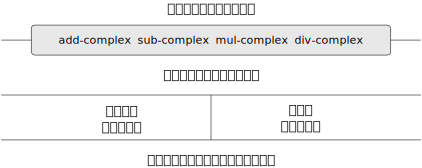
\includegraphics[width=108mm]{fig/chap2/Fig2.19a.pdf}
\begin{quote}
\heading{Figure 2.19:} Data-abstraction barriers in the complex-number system.
\end{quote}
\end{figure}

\noindent
In \link{Section 2.5} we will show how to use type tags and data-directed style
to develop a generic arithmetic package.  This provides procedures (\code{add},
\code{mul}, and so on) that can be used to manipulate all sorts of ``numbers''
and can be easily extended when a new kind of number is needed.  In 
\link{Section 2.5.3}, we'll show how to use generic arithmetic in a system that performs
symbolic algebra.

\link{Section 2.5}にてどのようにタイプタグとデータ適従スタイルを用いてジェネリックな数値演算パッケージを
開発するかについて示します。これは全ての種類の``数値''を操作するのに用いることができる手続(\code{add},
\code{mul}, その他)を提供します。\link{Section 2.5.3}ではどのようにして記号代数を実行するジェネリックな
数値演算をシステム内にて用いるかについて示します。


\label{Sec. 2.4.1}
\label{Section 2.4.1}
\subsection{Representations for Complex Numbers}

We will develop a system that performs arithmetic operations on complex numbers
as a simple but unrealistic example of a program that uses generic operations.
We begin by discussing two plausible representations for complex numbers as
ordered pairs: rectangular form (real part and imaginary part) and polar form
(magnitude and angle).\footnote{In actual computational systems, rectangular
form is preferable to polar form most of the time because of roundoff errors in
conversion between rectangular and polar form.  This is why the complex-number
example is unrealistic.  Nevertheless, it provides a clear illustration of the
design of a system using generic operations and a good introduction to the more
substantial systems to be developed later in this chapter.}  
\link{Section 2.4.2} will show how both representations can be made to coexist in a
single system through the use of type tags and generic operations.

ジェネリックな命令を用いる単純な代わりに非現実的なプログラムの例として複素数上で
数値演算命令を実行するシステムを開発します。順序有りペアとしての複素数に対する
2つのもっともらしい表現について議論することから始めます。直行形式(実数部と虚数部)と
極形式(大きさと角度)です。\footnote{実際の計算システムにおいては直行形式のほうが
極形式よりも多くの場合には好まれます。直行形式と極形式の間の変換における丸め誤差
のためです。これがなぜ複素数システムのサンプルが非現実的であるかの理由です。
それにもかかわらず、この例はジェネリック命令を用いたシステムの設計の明確な説明を
提供し、またこの章の中で後に開発されるより実質的なシステムに対する良い導入部で
あります。}
\link{Section 2.4.2}がどのようにして両方の表現がタイプタグとジェネリック命令の使用を通して
単一のシステム内にて共存できるように作成され得るのかについてを示します。

Like rational numbers, complex numbers are naturally represented as ordered
pairs.  The set of complex numbers can be thought of as a two-dimensional space
with two orthogonal axes, the ``real'' axis and the ``imaginary'' axis. (See
\link{Figure 2.20}.)  From this point of view, the complex number 
\( z = x + iy \) (where \( i^2 = -1 \)) can be thought of as the point in the plane
whose real coordinate is \( x \) and whose imaginary coordinate is \( y \).
Addition of complex numbers reduces in this representation to addition of
coordinates:

分数と同様に、複素数は自然に順序有りペアとして表現されます。複素数の集合は
2つの直行する軸を持つ二次元空間として考えることができます。この視点から複素数
\( z = x + iy \) (ここで \( i^2 = -1 \))はその平面中の実数座標が\( x \)かつ、
虚数座標が\( y \)の点として考えることが可能です。
複素数の和はこの表現において座標の和と還元できます。
\begin{comment}

\begin{example}
Real-part(z_1 + z_2) = Real-part(z_1) + Real-part(z_2)

Imaginary-part(z_1 + z_2) = Imaginary-part(z_1) + Imaginary-part(z_2)
\end{example}

\end{comment}
\begin{displaymath}
%  \eqalign{
% \hbox{Real-part} (z_1 + z_2)\; 		&= 
% 	\hbox{ Real-part} (z_1)\; + \hbox{ Real-part} (z_2), \cr
% \hbox{Imaginary-part} (z_1 + z_2)\; 	&= 
% 	\hbox{ Imaginary-part} (z_1)\; + \hbox{ Imaginary-part} (z_2). \cr 
% } 
\begin{array}{r@{{}={}}l}
  \hbox{Real-part} (z_1 + z_2)\; 	& 
	\hbox{ Real-part} (z_1)\; + \hbox{ Real-part} (z_2), \\
  \hbox{Imaginary-part} (z_1 + z_2)\; 	& 
	\hbox{ Imaginary-part} (z_1)\; + \hbox{ Imaginary-part} (z_2). 
\end{array}
\end{displaymath}

\begin{figure}[tb]
\phantomsection\label{Figure 2.20}
\centering
\begin{comment}
\heading{Figure 2.20:} Complex numbers as points in the plane.

\begin{example}
 Imaginary
    ^
    |
  y |.........................* z = x + ?y = r e^(?A)
    |                    __-- .
    |                __--     .
    |          r __--         .
    |        __--             .
    |    __-- \               .
    |__--    A |              .
----+----------+-------------------> Real
                              x
\end{example}
\end{comment}
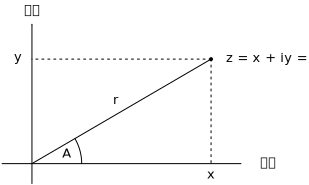
\includegraphics[width=79mm]{fig/chap2/Fig2.20.pdf}
\par\bigskip
\noindent
\heading{Figure 2.20:} Complex numbers as points in the plane.
\end{figure}

\noindent
When multiplying complex numbers, it is more natural to think in terms of
representing a complex number in polar form, as a magnitude and an angle (\( r \)
and \( A \) in \link{Figure 2.20}).  The product of two complex numbers is the
vector obtained by stretching one complex number by the length of the other and
then rotating it through the angle of the other:

複素数をかけ算する場合、複素数を大きさと角度(\link{Figure 2.20}内の\( r \)と\( A \))
としての極形式の表現を用いて考える方がより自然です。2つの複素数の積は一方の複素数を
もう一方の長さで延し次にもう一方の角度の分、回転することで得られるベクトルになります。
\begin{comment}

\begin{example}
Magnitude(z_1 * z_2) = Magnitude(z_1) * Magnitude(z_2)

Angle(z_1 * z_2) = Angle(z_1) + Angle(z_2)
\end{example}

\end{comment}
\begin{displaymath}
%  \eqalign{
% 	\hbox{Magnitude} (z_1 \cdot z_2)\; 	&= 
% 		\hbox{ Magnitude} (z_1)\; \cdot \hbox{ Magnitude} (z_2), \cr
% 	\hbox{Angle} (z_1 \cdot z_2)\; 		&= 
% 		\hbox{ Angle} (z_1)\; + \hbox{ Angle} (z_2). \cr
% } 
\begin{array}{r@{{}={}}l}
	\hbox{Magnitude} (z_1 \cdot z_2)\; 	& 
		\hbox{ Magnitude} (z_1)\; \cdot \hbox{ Magnitude} (z_2), \\
	\hbox{Angle} (z_1 \cdot z_2)\; 		& 
		\hbox{ Angle} (z_1)\; + \hbox{ Angle} (z_2). 
\end{array}
\end{displaymath}
\begin{displaymath}
\begin{array}{r@{{}={}}l}
	\hbox{大きさ} (z_1 \cdot z_2)\; 	&
		\hbox{ 大きさ} (z_1)\; \cdot \hbox{ 大きさ} (z_2), \\
	\hbox{角度} (z_1 \cdot z_2)\; 		&
		\hbox{ 角度} (z_1)\; + \hbox{ 角度} (z_2).
\end{array}
\end{displaymath}

\noindent
Thus, there are two different representations for complex numbers, which are
appropriate for different operations.  Yet, from the viewpoint of someone
writing a program that uses complex numbers, the principle of data abstraction
suggests that all the operations for manipulating complex numbers should be
available regardless of which representation is used by the computer.  For
example, it is often useful to be able to find the magnitude of a complex
number that is specified by rectangular coordinates.  Similarly, it is often
useful to be able to determine the real part of a complex number that is
specified by polar coordinates.

従って複素数には2つの異なる表現が存在し、それぞれは異なる操作に適しています。
けれども、複素数を用いるプログラムを書いている誰かさんの視点からは、データ抽象化の
主義が複素数を操作するための全ての命令はどの表現がコンピュータにより用いられるかに
係らず存在するべきだと提案します。例えば直行形式にて指定される複素数の大きさを
求められることはしばしば便利であります。同様に極形式にて指定される複素数の実数部を
決定できることも時折便利であります。

To design such a system, we can follow the same data-abstraction strategy we
followed in designing the rational-number package in \link{Section 2.1.1}.
Assume that the operations on complex numbers are implemented in terms of four
selectors: \code{real\-/part}, \code{imag\-/part}, \code{magnitude} and
\code{angle}.  Also assume that we have two procedures for constructing complex
numbers: \code{make\-/from\-/real\-/imag} returns a complex number with specified
real and imaginary parts, and \code{make\-/from\-/mag\-/ang} returns a complex number
with specified magnitude and angle.  These procedures have the property that,
for any complex number \code{z}, both

そのようなシステムを設計するために、\link{Section 2.1.1}にて分数パッケージの設計において従った
のと同じデータ抽象化戦略に従えます。複素数上の命令が4つのセレクタを使用して実装される
と想定します。\code{real\-/part}, \code{imag\-/part}, \code{magnitude}, \code{angle}です。
また複素数を構築する2つの手続を持っているとも想定します。\code{make\-/from\-/real\-/imag}は指定
された実数部と虚数部を持つ複素数を返し、\code{make\-/from\-/mag\-/ang}は指定された大きさと角度
を持つ複素数を返します。これらの手続は任意の複素数に対し同じ特性を持ちます。

\begin{scheme}
(make-from-real-imag (real-part z) (imag-part z))
\end{scheme}

\noindent
と

\begin{scheme}
(make-from-mag-ang (magnitude z) (angle z))
\end{scheme}

\noindent
produce complex numbers that are equal to \code{z}.

の両方が\code{z}に等しい複素数を生成します。

Using these constructors and selectors, we can implement arithmetic on complex
numbers using the ``abstract data'' specified by the constructors and
selectors, just as we did for rational numbers in \link{Section 2.1.1}.  As
shown in the formulas above, we can add and subtract complex numbers in terms
of real and imaginary parts while multiplying and dividing complex numbers in
terms of magnitudes and angles:

これらのコンストラクタとセレクタを用いて、\link{Section 2.1.1}で分数に対して行ったのと全く
同様に、コンストラクタとセレクタにて指定された``抽象データ''を用いて複素数上での
数値演算を実装可能です。前述の式にて示されたように、複素数の和と差は実数部と虚数部
を用いることで、また複素数の積と商は大きさと角度を用いることで実装できます。

\begin{scheme}
(define (add-complex z1 z2)
  (make-from-real-imag (+ (real-part z1) (real-part z2))
                       (+ (imag-part z1) (imag-part z2))))
\end{scheme}

\begin{scheme}
(define (sub-complex z1 z2)
  (make-from-real-imag (- (real-part z1) (real-part z2))
                       (- (imag-part z1) (imag-part z2))))
\end{scheme}

\begin{scheme}
(define (mul-complex z1 z2)
  (make-from-mag-ang (* (magnitude z1) (magnitude z2))
                     (+ (angle z1) (angle z2))))
\end{scheme}

\begin{scheme}
(define (div-complex z1 z2)
  (make-from-mag-ang (/ (magnitude z1) (magnitude z2))
                     (- (angle z1) (angle z2))))
\end{scheme}

\noindent
To complete the complex-number package, we must choose a representation and we
must implement the constructors and selectors in terms of primitive numbers and
primitive list structure.  There are two obvious ways to do this: We can
represent a complex number in ``rectangular form'' as a pair (real part,
imaginary part) or in ``polar form'' as a pair (magnitude, angle).  Which shall
we choose?

複素数パッケージを完了させるためには表現を選択し、コンストラクタとセレクタを
プリミティブな数値とリスト構造を用いて実装しなければなりません。これを行うために
2つ明らかな方法があります。``直行形式''の複素数はペア(実数部, 虚数部)として表現し、
また極形式はペア(大きさ, 角度)にて表現します。どちらを選択するべきでしょうか?

In order to make the different choices concrete, imagine that there are two
programmers, Ben Bitdiddle and Alyssa P. Hacker, who are independently
designing representations for the complex-number system.  Ben chooses to
represent complex numbers in rectangular form.  With this choice, selecting the
real and imaginary parts of a complex number is straightforward, as is
constructing a complex number with given real and imaginary parts.  To find the
magnitude and the angle, or to construct a complex number with a given
magnitude and angle, he uses the trigonometric relations

異なる選択を具体的にするために、二人のプログラマ、Ben BitdiddleとAlyssa P. Hacker
がいると想像して下さい。二人は複素数システムのための表現を独立して設計します。
Benは複素数を直行形式にて表現することを選択しました。この選択により現状として
複素数を与えられた実数部と虚数部から構築するため、実数部と虚数部を複素数から選択する
のは直接的です。大きさと角度を求めるためには、または複素数を与えられた大きさと角度から
構築するために彼は三角法の関係を用いました。
\begin{comment}

\begin{example}
                      __________
x = r cos A     r = ./ x^2 + y^2

y = r sin A     A = arctan(y,x)
\end{example}

\end{comment}
\begin{displaymath}
%  \eqalign{
% 	x = r \cos A, \qquad 	& r = \sqrt{x^2 + y^2}, \cr
% 	y = r \sin A, \qquad 	& A = \arctan(y, x), \cr
% } 
\begin{array}{r@{{}={}}lr@{{}={}}l}
	x & r \cos A, \qquad 	& r & \sqrt{x^2 + y^2}, \\
	y & r \sin A, \qquad 	& A & \arctan(y, x), 
\end{array}
\end{displaymath}
\noindent
which relate the real and imaginary parts \( (x, y) \) to the magnitude and
the angle \( (r, A) \).\footnote{The arctangent function referred to here,
computed by Scheme's \code{atan} procedure, is defined so as to take two
arguments \( y \) and \( x \) and to return the angle whose tangent is \( y \big/\! x \).
The signs of the arguments determine the quadrant of the angle.}  Ben's
representation is therefore given by the following selectors and constructors:

これは実数部と虚数部\( (x, y) \)を大きさと角度\( (r, A) \)へと関係づけます。\footnote{
ここで参照されたアークタンジェント関数は、Schemeの\code{atan}手続にて計算されますが、2つの
引数\( y \)と\( x \)を取りタンジェントが\( y / x \)となる角度を返すように定義
されました。引数の符号が角度の象限を決定します。}
Benの表現は従って以下のセレクタとコンストラクタにより与えられます。

\begin{scheme}
(define (real-part z) (car z))
(define (imag-part z) (cdr z))
(define (magnitude z)
  (sqrt (+ (square (real-part z))
           (square (imag-part z)))))
(define (angle z)
  (atan (imag-part z) (real-part z)))
(define (make-from-real-imag x y) (cons x y))
(define (make-from-mag-ang r a)
  (cons (* r (cos a)) (* r (sin a))))
\end{scheme}

\noindent
Alyssa, in contrast, chooses to represent complex numbers in polar form.  For
her, selecting the magnitude and angle is straightforward, but she has to use
the trigonometric relations to obtain the real and imaginary parts.  Alyssa's
representation is:

一方、Alyssaは複素数を極形式にて表現することを選択しました。彼女にとっては大きさと
角度を選択するのは直接的です。しかし実数部と虚数部を得るためには三角法の関係を用い
ねばなりません。Alyssaの表現は次のとおりです。

\begin{scheme}
(define (real-part z) (* (magnitude z) (cos (angle z))))
(define (imag-part z) (* (magnitude z) (sin (angle z))))
(define (magnitude z) (car z))
(define (angle z) (cdr z))
(define (make-from-real-imag x y)
  (cons (sqrt (+ (square x) (square y)))
        (atan y x)))
(define (make-from-mag-ang r a) (cons r a))
\end{scheme}

\noindent
The discipline of data abstraction ensures that the same implementation of
\code{add\-/complex}, \code{sub\-/complex}, \code{mul\-/complex}, and
\code{div\-/complex} will work with either Ben's representation or Alyssa's
representation.

データ抽象化の規律は\code{add\-/complex}, \code{sub\-/complex}, \code{mul\-/complex},
\code{div\-/complex}の同じ実装がBenの表現とAlyssaの表現のどちらに対してもうまく
いくことを保証します。

\label{Section 2.4.2}
\subsection{Tagged data}

One way to view data abstraction is as an application of the ``principle of
least commitment.''  In implementing the complex-number system in 
\link{Section 2.4.1}, we can use either Ben's rectangular representation or Alyssa's
polar representation.  The abstraction barrier formed by the selectors and
constructors permits us to defer to the last possible moment the choice of a
concrete representation for our data objects and thus retain maximum
flexibility in our system design.

データ抽象化を考え方の1つは``最小責務の原則''の適用としてです。\link{Section 2.4.1}の
複素数システムの実装において、私達はBenの直行形式表現とAlyssaの極形式表現の
どちらも使用することができました。セレクタとコンストラクタにより形成された
抽象化バリアが最後の可能な瞬間にデータオブジェクトに対する具体的な表現の
選択に従うことを可能にしています。従ってシステム設計において最高の柔軟性を
維持することができるのです。

The principle of least commitment can be carried to even further extremes.  If
we desire, we can maintain the ambiguity of representation even \emph{after} we
have designed the selectors and constructors, and elect to use both Ben's
representation \emph{and} Alyssa's representation.  If both representations are
included in a single system, however, we will need some way to distinguish data
in polar form from data in rectangular form.  Otherwise, if we were asked, for
instance, to find the \code{magnitude} of the pair (3, 4), we wouldn't know
whether to answer 5 (interpreting the number in rectangular form) or 3
(interpreting the number in polar form).  A straightforward way to accomplish
this distinction is to include a \newterm{type tag}---the symbol
\code{rectangular} or \code{polar}---as part of each complex number.  Then
when we need to manipulate a complex number we can use the tag to decide which
selector to apply.

最小責務の原則はさらにもっと高みへと到達することができます。もし私達が望めば、
セレクタとコンストラクタを設計した``後''にさえ表現の多義性を維持することが
可能です。そしてBenの表現``と''Alyssaの表現の両方の使用を選択できます。
もし両方の表現が単一のシステムに含まれる場合、極形式のデータを直行形式のデータから
識別するための何らかの方法が必要になります。そうでなけば、例えばペア(3, 4)の大きさ
を求めるよう尋ねられた場合に(数値を直行形式だと考えて)5と答えるべきか(数値が極形式
であると考えて)3と答えるべきであるのか分かりません。この識別を直接的な方法で達成する
ために\newterm{type tag}(タイプタグ)---\code{rectangular}または\code{polar}のシンボル---を
各複素数の部分として導入します。すると複素数を操作せねばならない時にタグを用いてどち
らのセレクタを適用するべきか決定することができます。

In order to manipulate tagged data, we will assume that we have procedures
\code{type\-/tag} and \code{contents} that extract from a data object the tag and
the actual contents (the polar or rectangular coordinates, in the case of a
complex number).  We will also postulate a procedure \code{attach\-/tag} that
takes a tag and contents and produces a tagged data object.  A straightforward
way to implement this is to use ordinary list structure:

タグ付きデータを操作するためにデータオブジェクトからタグと(複素数の場合には極形式、
または直行形式の)実際のコンテンツを抽出する手続\code{type\-/tag}と\code{contents}を持つと
想定します。またタグとコンテンツを取りタグ付きデータオブジェクトを生成する
手続\code{attach\-/tag}を仮定します。これを実装する直接的な方法は普通のリスト構造を用いる
ことです。

\begin{scheme}
(define (attach-tag type-tag contents)
  (cons type-tag contents))
(define (type-tag datum)
  (if (pair? datum)
      (car datum)
      (error "Bad tagged datum: TYPE-TAG" datum)))
(define (contents datum)
  (if (pair? datum)
      (cdr datum)
      (error "Bad tagged datum: CONTENTS" datum)))
\end{scheme}

\noindent
Using these procedures, we can define predicates \code{rectangular?}  and
\code{polar?}, which recognize rectangular and polar numbers, respectively:

これら手続を用いて述語\code{rectangular?}と\code{polar?}を定義し、直行形式と
極形式のそれぞれを認識することができます。

\begin{scheme}

(define (rectangular? z) (eq? (type-tag z) 'rectangular))
(define (polar? z) (eq? (type-tag z) 'polar))
\end{scheme}

\noindent
With type tags, Ben and Alyssa can now modify their code so that their two
different representations can coexist in the same system.  Whenever Ben
constructs a complex number, he tags it as rectangular.  Whenever Alyssa
constructs a complex number, she tags it as polar.  In addition, Ben and Alyssa
must make sure that the names of their procedures do not conflict.  One way to
do this is for Ben to append the suffix \code{rectangular} to the name of each
of his representation procedures and for Alyssa to append \code{polar} to the
names of hers.  Here is Ben's revised rectangular representation from 
\link{Section 2.4.1}:

タイプタグを用いてBenとAlyssaはこれで彼等のコードを変更し2つの異なる表現が同じ
システム内にて共存させることができるようになりました。Benが複素数を構築する度に
彼は直行形式であるとタグを付けます。Alyssaが複素数を構築する度に、彼女はそれを
極形式であるとタグを付けます。加えて、BenとAlyssaは手続の名前が衝突しないように
確認しなければなりません。これを行う1つの方法としてBenは彼の各表現手続に接尾辞
\code{rectangular}を追加し、Alyssaは彼女の手続に対し\code{polar}を付け加えます。
以下はBenの\link{Section 2.4.1}から改正した直行形式表現です。

\begin{scheme}
(define (real-part-rectangular z) (car z))
(define (imag-part-rectangular z) (cdr z))
(define (magnitude-rectangular z)
  (sqrt (+ (square (real-part-rectangular z))
           (square (imag-part-rectangular z)))))
(define (angle-rectangular z)
  (atan (imag-part-rectangular z)
        (real-part-rectangular z)))
(define (make-from-real-imag-rectangular x y)
  (attach-tag 'rectangular (cons x y)))
(define (make-from-mag-ang-rectangular r a)
  (attach-tag 'rectangular
              (cons (* r (cos a)) (* r (sin a)))))
\end{scheme}

\noindent
and here is Alyssa's revised polar representation:

そして以下はAlyssaの改訂版極形式表現です。

\begin{scheme}
(define (real-part-polar z)
  (* (magnitude-polar z) (cos (angle-polar z))))
(define (imag-part-polar z)
  (* (magnitude-polar z) (sin (angle-polar z))))
(define (magnitude-polar z) (car z))
(define (angle-polar z) (cdr z))

(define (make-from-real-imag-polar x y)
  (attach-tag 'polar
              (cons (sqrt (+ (square x) (square y)))
                    (atan y x))))
(define (make-from-mag-ang-polar r a)
  (attach-tag 'polar (cons r a)))
\end{scheme}

\noindent
Each generic selector is implemented as a procedure that checks the tag of its
argument and calls the appropriate procedure for handling data of that type.
For example, to obtain the real part of a complex number, \code{real\-/part}
examines the tag to determine whether to use Ben's \code{real\-/part\-/rectangular}
or Alyssa's \code{real\-/part\-/polar}.  In either case, we use \code{contents} to
extract the bare, untagged datum and send this to the rectangular or polar
procedure as required:

各ジェネリックなセレクタは引数のタグをチェックし、そのタイプのデータを扱うのに
適切な手続を呼び出す様に実装されます。例として、複素数の実数部を得る場合、
\code{real\-/part}はタグを確かめBenの\code{real\-/part\-/rectangular}かAlyssaの\code{real\-/part\-/polar}の
どちらを使うのかを決定します。どちらの場合でも\code{contents}を用いて生のタグの無いデータを
抽出し直交形式、または極形式の手続を必要に応じて呼び出します。

\begin{scheme}
(define (real-part z)
  (cond ((rectangular? z)
         (real-part-rectangular (contents z)))
        ((polar? z)
         (real-part-polar (contents z)))
        (else (error "Unknown type: REAL-PART" z))))

(define (imag-part z)
  (cond ((rectangular? z)
         (imag-part-rectangular (contents z)))
        ((polar? z)
         (imag-part-polar (contents z)))
        (else (error "Unknown type: IMAG-PART" z))))

(define (magnitude z)
  (cond ((rectangular? z)
         (magnitude-rectangular (contents z)))
        ((polar? z)
         (magnitude-polar (contents z)))
        (else (error "Unknown type: MAGNITUDE" z))))
(define (angle z)
  (cond ((rectangular? z)
         (angle-rectangular (contents z)))
        ((polar? z)
         (angle-polar (contents z)))
        (else (error "Unknown type: ANGLE" z))))
\end{scheme}

\noindent
To implement the complex-number arithmetic operations, we can use the same
procedures \code{add\-/complex}, \code{sub\-/complex}, \code{mul\-/complex}, and
\code{div\-/complex} from \link{Section 2.4.1}, because the selectors they call
are generic, and so will work with either representation.  For example, the
procedure \code{add\-/complex} is still

複素数演算命令を実装するためには\link{Section 2.4.1}から同じ手続\code{add\-/complex}, 
\code{sub\-/complex}, \code{mul\-/complex}, \code{div\-/complex}を使うことができます。
なぜならそれらが呼び出すセレクタはジェネリックであるためどちらの表現に対して
も働くからです。例として手続\code{add\-/complex}は今でも以下のとおりです。

\begin{scheme}
(define (add-complex z1 z2)
  (make-from-real-imag (+ (real-part z1) (real-part z2))
                       (+ (imag-part z1) (imag-part z2))))
\end{scheme}

\noindent
Finally, we must choose whether to construct complex numbers using Ben's
representation or Alyssa's representation.  One reasonable choice is to
construct rectangular numbers whenever we have real and imaginary parts and to
construct polar numbers whenever we have magnitudes and angles:

最後に、複素数をBenの表現とAlyssaの表現のどちらを利用して構築するのか決定
しなければなりません。妥当な選択として実数部と虚数部がある場合には直行形式を
用い、大きさと角度がある場合には極形式を用いて構築します。

\begin{scheme}
(define (make-from-real-imag x y)
  (make-from-real-imag-rectangular x y))
(define (make-from-mag-ang r a)
  (make-from-mag-ang-polar r a))
\end{scheme}

\noindent
The resulting complex-number system has the structure shown in \link{Figure 2.21}.  
The system has been decomposed into three relatively independent parts:
the complex-number-arithmetic operations, Alyssa's polar implementation, and
Ben's rectangular implementation.  The polar and rectangular implementations
could have been written by Ben and Alyssa working separately, and both of these
can be used as underlying representations by a third programmer implementing
the complex-arithmetic procedures in terms of the abstract constructor/selector
interface.

結果としての複素数システムは\link{Figure 2.21}にて表される構造を持ちます。
システムは3つの関連する独立した部分に分離されます。複素数演算命令、Alyssaの
極形式実装、そしてBenの直行形式実装です。極形式と直行形式の実装はBenとAlyssaが
別々に働きながら書かれることが可能でした。そして両者が
抽象コンストラクタ、セレクタのインターフェイスを用いながら複素数演算手続を実装する
第三者のプログラマにより基礎を成す表現として利用されることが可能です。

\begin{figure}[tb]
\phantomsection\label{Figure 2.21}
\centering
\begin{comment}
\begin{quote}
\heading{Figure 2.21:} Structure of the generic complex-arithmetic system.

\begin{example}
    +-------------------------------------------------+
----| add-complex sub-complex mul-complex div-complex |----
    +-------------------------------------------------+
                Complex arithmetic package
                 +-----------------------+
                 | real-part   imag-part |
-----------------|                       |------------------
                 | magnitude   angle     |
                 +-----------+-----------+
           Rectangular       |          Polar
          representation     |     representation
-----------------------------+------------------------------
       List structure and primitive machine arithmetic
\end{example}
\end{quote}
\end{comment}
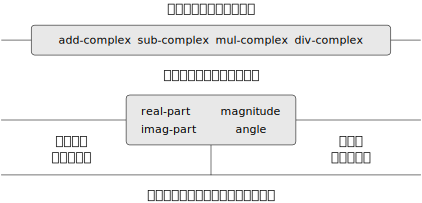
\includegraphics[width=108mm]{fig/chap2/Fig2.21a.pdf}
\begin{quote}
\heading{Figure 2.21:} Structure of the generic complex-arithmetic system.
\end{quote}
\end{figure}

\noindent
Since each data object is tagged with its type, the selectors operate on the
data in a generic manner.  That is, each selector is defined to have a behavior
that depends upon the particular type of data it is applied to.  Notice the
general mechanism for interfacing the separate representations: Within a given
representation implementation (say, Alyssa's polar package) a complex number is
an untyped pair (magnitude, angle).  When a generic selector operates on a
number of \code{polar} type, it strips off the tag and passes the contents on
to Alyssa's code.  Conversely, when Alyssa constructs a number for general use,
she tags it with a type so that it can be appropriately recognized by the
higher-level procedures.  This discipline of stripping off and attaching tags
as data objects are passed from level to level can be an important
organizational strategy, as we shall see in \link{Section 2.5}.

各データオブジェクトはその型にてタグ付けられているので、セレクタはデータに対し
ジェネリックな方法で操作します。これは各セレクタがそれが適用される個々のデータの
型に従う振舞を持つように定義されているということです。分けられた表現を結び付ける
ための一般的なメカニズムについて注意して下さい。与えられた表現実装(例えばAlyssaの
極形式パッケージ)の中では複素数は型の無いペア(大きさ, 角度)です。ジェネリックな
セレクタが極形式の型(タイプ)の複素数を操作する時、タグを取り中身をAlyssaのコードに
渡します。反対にAlyssaが通常の使用のために数値を構築する時、彼女が型でタグを付ける
ことでより高いレベルの手続により適切に認識されることができます。データオブジェクトが
あるレベルから別のレベルへと渡されるに従い、このタグの取り付けと除去の規律が重要な
組織的戦略となります。\link{Section 2.5}にてこれについて学びます。


\label{Section 2.4.3}
\subsection{Data-Directed Programming and Additivity}

The general strategy of checking the type of a datum and calling an appropriate
procedure is called \newterm{dispatching on type}.  This is a powerful strategy
for obtaining modularity in system design.  On the other hand, implementing the
dispatch as in \link{Section 2.4.2} has two significant weaknesses.  One
weakness is that the generic interface procedures (\code{real\-/part},
\code{imag\-/part}, \code{magnitude}, and \code{angle}) must know about all the
different representations.  For instance, suppose we wanted to incorporate a
new representation for complex numbers into our complex-number system.  We
would need to identify this new representation with a type, and then add a
clause to each of the generic interface procedures to check for the new type
and apply the appropriate selector for that representation.

データの型をチェックし適切な手続を呼ぶ一般的な戦略は
\newterm{dispatching on type}(タイプ別処理)と呼ばれる。これはシステム設計において
モジュール方式を得るための強力な戦略です。一方で\link{Section 2.4.2}のような呼出の実装は
2つの明らかな弱点が存在します。1つはジェネリックインターフェイス手続(\code{real\-/part},
\code{imag\-/part}, \code{magnitude}, \code{angle})は全ての異なる表現について知っていなければ
なりません。例えば複素数に対する新しい表現を複素数システムに組み入れたいとしましょう。
この新しい表現を型にて識別し、次に全てのジェネリックインターフェイス手続に新しい型を
チェックする条項を追加し、その表現に対する適切なセレクタを適用する必要が出てくるでしょう。

Another weakness of the technique is that even though the individual
representations can be designed separately, we must guarantee that no two
procedures in the entire system have the same name.  This is why Ben and Alyssa
had to change the names of their original procedures from 
\link{Section 2.4.1}.

もう1つのこのテクニックの弱点は例え個々の表現が別々に設計できたとしても、システム全体の
中でどの2つの手続も同じ名前を持たないことを保証せねばなりません。これがなぜBenとAlyssa
が\link{Section 2.4.1}の彼等の元の手続の名前を変更しなければいけないかの理由でした。

The issue underlying both of these weaknesses is that the technique for
implementing generic interfaces is not \newterm{additive}.  The person
implementing the generic selector procedures must modify those procedures each
time a new representation is installed, and the people interfacing the
individual representations must modify their code to avoid name conflicts.  In
each of these cases, the changes that must be made to the code are
straightforward, but they must be made nonetheless, and this is a source of
inconvenience and error.  This is not much of a problem for the complex-number
system as it stands, but suppose there were not two but hundreds of different
representations for complex numbers.  And suppose that there were many generic
selectors to be maintained in the abstract-data interface.  Suppose, in fact,
that no one programmer knew all the interface procedures or all the
representations.  The problem is real and must be addressed in such programs as
large-scale data-base-management systems.

両者の弱点の根底にある問題はジェネリックインターフェイスを実装するためのテクニック
が\newterm{additive}(付加的)でないことです。ジェネリックセレクタ手続を実装する人は
これらの手続を新しい表現がインストールされる度に変更せねばならず、また個々の表現を
接続する人々は名前衝突が起こらぬ様に彼等のコードを変更せねばなりません。
これらのケースのそれぞれでコードに対して加えられなければならない変更は簡単ですが、
それでも必ず行わねばならず、不自由さと障害の原因となります。これは複素数システムに
対しては現時点ではあまり大きな問題ではありません。しかしただ2つではなく数百もの異なる
表現が複素数に対して存在すると仮定してみて下さい。その上どのプログラマも全ての
インターフェイス手続や全ての表現について知らないと想定してみて下さい。問題は現実的で
あり大規模なデータベース管理システムのようなプログラムでは必ず解決される必要があります。

What we need is a means for modularizing the system design even further.  This
is provided by the programming technique known as \newterm{data-directed
programming}.  To understand how data-directed programming works, begin with
the observation that whenever we deal with a set of generic operations that are
common to a set of different types we are, in effect, dealing with a
two-dimensional table that contains the possible operations on one axis and the
possible types on the other axis.  The entries in the table are the procedures
that implement each operation for each type of argument presented.  In the
complex-number system developed in the previous section, the correspondence
between operation name, data type, and actual procedure was spread out among
the various conditional clauses in the generic interface procedures.  But the
same information could have been organized in a table, as shown in \link{Figure 2.22}.

私達に必要なものはより一層のシステム設計のモジュール化のための手段です。
これは\newterm{data-directed programming}(データ適従プログラミング)として知られる
プログラミングテクニックにより提供されます。データ適従プログラミングがどのように
働くかを理解するためには、
異なる型の集合に対して共通なジェネリックな命令の集合を扱う度に、
実際に予想される命令を1つの軸に、予想される型をもう一方の軸に持つ二次元の表に取り組み、
その観察結果から始めます。
表の項目には与えられた各引数の型に対する各命令を実装する手続です。
前の章にて開発された複素数システムでは命令の名前、データタイプ、実際の手続の間の対応は
ジェネリックなインターフェイス手続の種々の条件節の間に広がっています。
しかし同じ情報が\link{Figure 2.22}の中に示されるように1つのテーブルの中に組込まれることが
できたはずです。

Data-directed programming is the technique of designing programs to work with
such a table directly.  Previously, we implemented the mechanism that
interfaces the complex-arithmetic code with the two representation packages as
a set of procedures that each perform an explicit dispatch on type.  Here we
will implement the interface as a single procedure that looks up the
combination of the operation name and argument type in the table to find the
correct procedure to apply, and then applies it to the contents of the
argument.  If we do this, then to add a new representation package to the
system we need not change any existing procedures; we need only add new entries
to the table.

データ適従プログラミングはそのようなテーブルと直接連携するためのプログラム設計の
テクニックです。以前は私達は複素数演算コードをそれぞれが明示的に型に従う呼び出し
を行う手続の集合としての2つの表現パッケージと接続するメカニズムを実装しました。
ここではインターフェイスを命令の名前と引数タイプの組み合わせをテーブルの中から調べ
適用すべき正しい手続を見つける単一の手続として実装します。そして次にその手続を
引数の中身に対して適用します。これを行なえば、システムに対して新しい
表現パッケージの追加するために既存の手続に何の変更を行う必要もありません。
必要なのは表に新しい項目を追加することです。

\begin{figure}[tb]
\phantomsection\label{Figure 2.22}
\centering
\begin{comment}
\begin{quote}
\heading{Figure 2.22:} Table of operations for the complex-number system.

\begin{example}
           |               Types
Operations | Polar           | Rectangular
===========+=================+======================
real-part  | real-part-polar | real-part-rectangular
imag-part  | imag-part-polar | imag-part-rectangular
magnitude  | magnitude-polar | magnitude-rectangular
angle      | angle-polar     | angle-rectangular
\end{example}
\end{quote}
\end{comment}
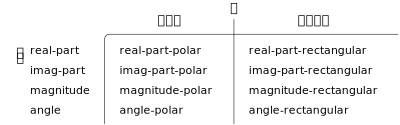
\includegraphics[width=102mm]{fig/chap2/Fig2.22.pdf}
\begin{quote}
\heading{Figure 2.22:} Table of operations for the complex-number system.
\end{quote}
\end{figure}

\noindent
To implement this plan, assume that we have two procedures, \code{put} and
\code{get}, for manipulating the operation-and-type table:

この計画を実装するために、2つの手続\code{put}と\code{get}を命令と型のテーブルを操作するために
持っていると仮定します。

\begin{itemize}

\item
\( \hbox{\tt(put}\;\langle \)\var{op}\( \kern0.1em\rangle\;\langle \)\var{type}\( \kern0.08em\rangle\;\langle \)\var{item}\( \kern0.08em\rangle\hbox{\tt)} \) installs the \( \langle \)\var{item}\( \kern0.08em\rangle \) in the table, indexed by the
\( \langle \)\var{op}\( \kern0.1em\rangle \) and the \( \langle \)\var{type}\( \kern0.08em\rangle \).

\item
\( \hbox{\tt(get}\;\langle \)\var{op}\( \kern0.1em\rangle\;\langle \)\var{type}\( \kern0.08em\rangle\hbox{\tt)} \) looks up the
\( \langle \)\var{op}\( \kern0.08em\rangle \), \( \langle \)\var{type}\( \kern0.08em\rangle \) entry in the table and
returns the item found there.  If no item is found, \code{get} returns false.

\item
\( \hbox{\tt(put}\;\langle \)\var{op}\( \kern0.1em\rangle\;\langle \)\var{type}\( \kern0.08em\rangle\;\langle \)\var{item}\( \kern0.08em\rangle\hbox{\tt)} \)は\( \langle \)\var{item}\( \kern0.08em\rangle \)をテーブルに挿入し、
\( \langle \)\var{op}\( \kern0.1em\rangle \)と\( \langle \)\var{type}\( \kern0.08em\rangle \)で索引付けられる

\item
\( \hbox{\tt(get}\;\langle \)\var{op}\( \kern0.1em\rangle\;\langle \)\var{type}\( \kern0.08em\rangle\hbox{\tt)} \)は
\( \langle \)\var{op}\( \kern0.08em\rangle \), \( \langle \)\var{type}\( \kern0.08em\rangle \)の項目をテーブルから探し
見つかった項目を返す。 もし見つからない場合には\code{get}はfalseを返す

\end{itemize}

\noindent
For now, we can assume that \code{put} and \code{get} are included in our
language.  In \link{Chapter 3} (\link{Section 3.3.3}) we
will see how to implement these and other operations for manipulating tables.

今のところは\code{put}と\code{get}が私達の言語に含まれていると仮定しましょう。
\link{Chapter 3} (\link{Section 3.3.3})においてこれらと他のテーブル操作の命令をどのように実装するか
について学びます。

Here is how data-directed programming can be used in the complex-number system.
Ben, who developed the rectangular representation, implements his code just as
he did originally.  He defines a collection of procedures, or a
\newterm{package}, and interfaces these to the rest of the system by adding
entries to the table that tell the system how to operate on rectangular
numbers.  This is accomplished by calling the following procedure:

ここからはデータ適従プログラミングが複素数システムにおいてどのように使用できるかについて
示します。直行形式表現を開発したBenは彼が元々行ったとおりにコードを実装しました。
彼は手続の集合、つまりは\newterm{package}(パッケージ)を定義し、システムに
どのように直行形式の数値を取り扱うかを教えるテーブルに項目を追加する
ことで、パッケージをシステムの残りに対して接続します。
これは以下の手続を呼び出すことにより達成されます。

\begin{scheme}
(define (install-rectangular-package)
  ~\textrm{;; internal procedures}~
  (define (real-part z) (car z))
  (define (imag-part z) (cdr z))
  (define (make-from-real-imag x y) (cons x y))
  (define (magnitude z)
    (sqrt (+ (square (real-part z))
             (square (imag-part z)))))
  (define (angle z)
    (atan (imag-part z) (real-part z)))
  (define (make-from-mag-ang r a)
    (cons (* r (cos a)) (* r (sin a))))

  ~\textrm{;; interface to the rest of the system}~
  (define (tag x) (attach-tag 'rectangular x))
  (put 'real-part '(rectangular) real-part)
  (put 'imag-part '(rectangular) imag-part)
  (put 'magnitude '(rectangular) magnitude)
  (put 'angle '(rectangular) angle)
  (put 'make-from-real-imag 'rectangular
       (lambda (x y) (tag (make-from-real-imag x y))))
  (put 'make-from-mag-ang 'rectangular
       (lambda (r a) (tag (make-from-mag-ang r a))))
  'done)
\end{scheme}

\noindent
Notice that the internal procedures here are the same procedures from 
\link{Section 2.4.1} that Ben wrote when he was working in isolation.  No changes are
necessary in order to interface them to the rest of the system.  Moreover,
since these procedure definitions are internal to the installation procedure,
Ben needn't worry about name conflicts with other procedures outside the
rectangular package.  To interface these to the rest of the system, Ben
installs his \code{real\-/part} procedure under the operation name
\code{real\-/part} and the type \code{(rectangular)}, and similarly for the other
selectors.\footnote{We use the list \code{(rectangular)} rather than the symbol
\code{rectangular} to allow for the possibility of operations with multiple
arguments, not all of the same type.}  The interface also defines the
constructors to be used by the external system.\footnote{The type the
constructors are installed under needn't be a list because a constructor is
always used to make an object of one particular type.}  These are identical to
Ben's internally defined constructors, except that they attach the tag.

この中の内部手続はBenが\link{Section 2.4.1}にて分離を行った時に彼が書いたものと同じ
手続であることに注意して下さい。これらをシステムの残りに接続するためには
全く変更が必要がありません。さらに、これらの手続の定義はインストールを行う
手続の内部であるため、Benは直行形式パッケージの外部の他の手続に対して
名前の衝突が起こることを全く心配する必要がありません。
これらをシステムの残りに対し接続するために、Benは彼の\code{real\-/part}手続を
命令名\code{real\-/part}と型\code{(rectangular)}の元にインストールしました。
そして他のセレクタに対しても同様に行いました。\footnote{
私達はシンボル\code{rectangular}ではなくリスト\code{(rectangular)}を用いました。
全てが同じ型ではない複数の引数を伴なう命令の可能性を考慮するためです。}
このインターフェイスはまた外部システムにより利用されるコンストラクタも
定義します。\footnote{コンストラクタがその下にインストールされる型は
リストである必要がありません。なぜならコンストラクタは常にある特定の型の
オブジェクトを作成するために使用されるためです。}これらはBenの内部定義
コンストラクタと全く同じです。ただしタグを付加することが異なります。

Alyssa's polar package is analogous:

Alyassaの極形式パッケージも同様です。

\begin{scheme}
(define (install-polar-package)
  ~\textrm{;; internal procedures}~
  (define (magnitude z) (car z))
  (define (angle z) (cdr z))
  (define (make-from-mag-ang r a) (cons r a))
  (define (real-part z)
    (* (magnitude z) (cos (angle z))))
  (define (imag-part z)
    (* (magnitude z) (sin (angle z))))
  (define (make-from-real-imag x y)
    (cons (sqrt (+ (square x) (square y)))
          (atan y x)))
  ~\textrm{;; interface to the rest of the system}~
  (define (tag x) (attach-tag 'polar x))
  (put 'real-part '(polar) real-part)
  (put 'imag-part '(polar) imag-part)
  (put 'magnitude '(polar) magnitude)
  (put 'angle '(polar) angle)
  (put 'make-from-real-imag 'polar
       (lambda (x y) (tag (make-from-real-imag x y))))
  (put 'make-from-mag-ang 'polar
       (lambda (r a) (tag (make-from-mag-ang r a))))
  'done)
\end{scheme}

\noindent
Even though Ben and Alyssa both still use their original procedures defined
with the same names as each other's (e.g., \code{real\-/part}), these definitions
are now internal to different procedures (see \link{Section 1.1.8}), so there is
no name conflict.

BenとAlyssaの両者が今でも御互いに同じ名前(例えば\code{real\-/part})にて定義された
彼等の元々の手続を使用してようとも、これらの定義は今では異なる手続の内部定義(\link{Section 1.1.8}参照)
です。従って名前の衝突は起こりません。

The complex-arithmetic selectors access the table by means of a general
``operation'' procedure called \code{apply\-/generic}, which applies a generic
operation to some arguments.  \code{Apply\-/generic} looks in the table under the
name of the operation and the types of the arguments and applies the resulting
procedure if one is present:

複素数演算のセレクタは\code{apply\-/generic}と呼ばれる普遍的な``operation''手続を
用いてテーブルにアクセスします。これはジェネリックな命令を引数に対して適用します。
\code{apply\-/generic}は命令の名前と引数の型の下に表を調べ結果としての手続が存在すれば
適用します。\footnote{
\code{Apply\-/generic} uses the dotted-tail
notation described in \link{Exercise 2.20}, because different generic operations
may take different numbers of arguments.  In \code{apply\-/generic}, \code{op}
has as its value the first argument to \code{apply\-/generic} and \code{args} has
as its value a list of the remaining arguments.

\code{apply\-/generic}は\link{Exercise 2.20}で説明したドット付き
末尾記法を用います。異なるジェネリック命令は異なる数の引数を取る場合が考えられる
ためです。\code{apply\-/generic}では\code{op}がその値として\code{apply\-/generic}の第一引数を
持ち、\code{args}はその値として残りの引数のリストを持ちます。

\code{Apply\-/generic} also uses the primitive procedure \code{apply}, which
takes two arguments, a procedure and a list.  \code{Apply} applies the
procedure, using the elements in the list as arguments.  For example,

\code{apply\-/generic}はまたプリミティブな手続\code{apply}を用います。これは2つの引数、
手続とリストを取ります。\code{apply}はリストの要素を引数として手続を適用します。
例えば、

\begin{smallscheme}
(apply + (list 1 2 3 4))
\end{smallscheme}

\noindent
returns 10.

は10を返します。}

\begin{scheme}
(define (apply-generic op . args)
  (let ((type-tags (map type-tag args)))
    (let ((proc (get op type-tags)))
      (if proc
          (apply proc (map contents args))
          (error
            "No method for these types: APPLY-GENERIC"
            (list op type-tags))))))
\end{scheme}

\noindent
Using \code{apply\-/generic}, we can define our generic selectors as follows:

\code{apply\-/generic}を用いることで、私達のジェネリックなセレクタを以下のように定義する
ことができます。

\begin{scheme}
(define (real-part z) (apply-generic 'real-part z))
(define (imag-part z) (apply-generic 'imag-part z))
(define (magnitude z) (apply-generic 'magnitude z))
(define (angle z) (apply-generic 'angle z))
\end{scheme}

\noindent
Observe that these do not change at all if a new representation is added to the
system.

もし新しい表現がシステムに追加されたとしてもこれらが全く変更されないことに注意して
下さい。

We can also extract from the table the constructors to be used by the programs
external to the packages in making complex numbers from real and imaginary
parts and from magnitudes and angles.  As in \link{Section 2.4.2}, we construct
rectangular numbers whenever we have real and imaginary parts, and polar
numbers whenever we have magnitudes and angles:

またテーブルからコンストラクタを抽出することもできます。コンストラクタはパッケージの
外部プログラムにより使用でき、実数部と虚数部か大きさと角度から複素数を作ります。
\link{Section 2.4.2}にあるとおり、実数部と虚数部がある場合には直交形式で構築し、大きさと
角度がある場合には極形式にて構築します。

\begin{scheme}
(define (make-from-real-imag x y)
  ((get 'make-from-real-imag 'rectangular) x y))
(define (make-from-mag-ang r a)
  ((get 'make-from-mag-ang 'polar) r a))
\end{scheme}

\begin{quote}
\heading{\phantomsection\label{Exercise 2.73}Exercise 2.73:} \link{Section 2.3.2} described a
program that performs symbolic differentiation:

\link{Section 2.3.2}は記号微分を行うプログラムについて説明した。

\begin{scheme}
(define (deriv exp var)
  (cond ((number? exp) 0)
        ((variable? exp) 
         (if (same-variable? exp var) 1 0))
        ((sum? exp)
         (make-sum (deriv (addend exp) var)
                   (deriv (augend exp) var)))
        ((product? exp)
         (make-sum (make-product
                    (multiplier exp)
                    (deriv (multiplicand exp) var))
                   (make-product 
                    (deriv (multiplier exp) var)
                    (multiplicand exp))))
        ~\( \dark \langle \)~~\var{\dark more rules can be added here}~~\( \dark \rangle \)~
        (else (error "unknown expression type: 
                      DERIV" exp))))
\end{scheme}

We can regard this program as performing a dispatch on the type of the
expression to be differentiated.  In this situation the ``type tag'' of the
datum is the algebraic operator symbol (such as \code{+}) and the operation
being performed is \code{deriv}.  We can transform this program into
data-directed style by rewriting the basic derivative procedure as

このプログラムを微分する式のタイプにより呼出を行っていると解釈することもできる。
このシチュエーションではデータの``タイプタグ''が代数演算子の記号(例えば\code{+})であり
実行される命令は\code{deriv}である。このプログラムを基本の微分手続を書き直すことで
データ適従プログラミングスタイルに変換することができる。

\begin{scheme}
(define (deriv exp var)
  (cond ((number? exp) 0)
        ((variable? exp) 
         (if (same-variable? exp var) 1 0))
        (else ((get 'deriv (operator exp)) 
               (operands exp) var))))
(define (operator exp) (car exp))
(define (operands exp) (cdr exp))
\end{scheme}

\begin{enumerate}[a]

\item
Explain what was done above.  Why can't we assimilate the predicates
\code{number?} and \code{variable?} into the data-directed dispatch?

上で何が行われたのか説明せよ。なぜ手続\code{number?}と\code{variable?}をデータ適従呼出に
吸収することができないのか?

\item
Write the procedures for derivatives of sums and products, and the auxiliary
code required to install them in the table used by the program above.

和と積の微分のための手続とそれらを上記のプログラムで使用されたテーブルにインストールする
補助コードを書け。

\item
Choose any additional differentiation rule that you like, such as the one for
exponents (\link{Exercise 2.56}), and install it in this data-directed
system.

貴方の好きな追加の微分ルール、例えば指数に対する物(\link{Exercise 2.56})を選択し、
このデータ適従システムにインストールせよ。

\item
In this simple algebraic manipulator the type of an expression is the algebraic
operator that binds it together.  Suppose, however, we indexed the procedures
in the opposite way, so that the dispatch line in \code{deriv} looked like

この単純な代数操作において、式の型はそれを一緒に束縛する代数演算子である。
しかし手続を逆の向きに索引付けし\code{deriv}の呼出行を以下のようにした場合、

\begin{scheme}
((get (operator exp) 'deriv) (operands exp) var)
\end{scheme}

\noindent
What corresponding changes to the derivative system are required?

微分システムへの対応する変更は何が必要か?

\end{enumerate}
\end{quote}

\begin{quote}
\heading{\phantomsection\label{Exercise 2.74}Exercise 2.74:} Insatiable Enterprises, Inc., is
a highly decentralized conglomerate company consisting of a large number of
independent divisions located all over the world.  The company's computer
facilities have just been interconnected by means of a clever
network-interfacing scheme that makes the entire network appear to any user to
be a single computer.  Insatiable's president, in her first attempt to exploit
the ability of the network to extract administrative information from division
files, is dismayed to discover that, although all the division files have been
implemented as data structures in Scheme, the particular data structure used
varies from division to division.  A meeting of division managers is hastily
called to search for a strategy to integrate the files that will satisfy
headquarters' needs while preserving the existing autonomy of the divisions.

Insatiable Enterprises, Inc.(強欲エンタープライズ社)は高いレベルで非集中化された
数多くの独立事業所を世界中に抱える複合企業である。社のコンピュータ施設は接続された
ばかりであるが、賢いネットワーク接続計画を用いてネットワーク全体がどのユーザに対し
ても1台のコンピュータとして現れる。強欲社の社長は初めてネットワークの機能を用い
て事業所ファイルから管理者情報を取得しようと試みたが、全ての事業所ファイルは
Schemeのデータ構造として実装されているのにも係らず、使用されている個々のデータ構造は
事業所の間で異なっていることに狼狽した。事業所長の会議が大急ぎで開催され既存の事業所の
自立性を保ちつつ本社の要求を満足できるファイル統合の戦略を探すことになった。

Show how such a strategy can be implemented with data-directed programming.  As
an example, suppose that each division's personnel records consist of a single
file, which contains a set of records keyed on employees' names.  The structure
of the set varies from division to division.  Furthermore, each employee's
record is itself a set (structured differently from division to division) that
contains information keyed under identifiers such as \code{address} and
\code{salary}.  In particular:

そのような戦略がデータ適従戦略を用いてどのように実装できるか示せ。例として各事業所
の職員記録は単一のファイルから成る従業員の名前をキーにしたレコードの集合であると
想定せよ。集合の構造は事業所毎に変わる。さらに各従業員のレコードはそれ自身が集合
(事業所毎で異なる構造)であり\code{address}と\code{salary}のような識別子の下で鍵付けられた
情報を含んでいる。具体的には

\begin{enumerate}[a]

\item
Implement for headquarters a \code{get\-/record} procedure that retrieves a
specified employee's record from a specified personnel file.  The procedure
should be applicable to any division's file.  Explain how the individual
divisions' files should be structured.  In particular, what type information
must be supplied?

本社のために指定された従業員のレコードを指定された職員記録ファイルから取得する
\code{get\-/record}手続を実装せよ。手続は任意の事業所のファイルに適用できなければならない。
個々の事業所のファイルがどのように構造化されねばならないか説明せよ。
具体的にはどんな型の情報が提供されねばならないか

\item
Implement for headquarters a \code{get\-/salary} procedure that returns the
salary information from a given employee's record from any division's personnel
file.  How should the record be structured in order to make this operation
work?

本社のために任意の事業所の職員記録ファイルから与えられた職員記録から給与情報を返す
\code{get\-/salary}手続を実装せよ。
記録はこの操作が動くようどのように構造化されねばならないか?

\item
Implement for headquarters a \code{find\-/employee\-/record} procedure.  This
should search all the divisions' files for the record of a given employee and
return the record.  Assume that this procedure takes as arguments an employee's
name and a list of all the divisions' files.

本社のために\code{find\-/employee\-/record} 手続を実装せよ。これは全ての事業所のファイルに対し
与えられた従業員のレコードを探し、レコードを返さねばならない。この手続が引数として
従業員の名前と全ての事業所のファイルのリストを与えられると仮定せよ。

\item
When Insatiable takes over a new company, what changes must be made in order to
incorporate the new personnel information into the central system?

強欲社が新しい会社を吸収した時、どんな変更が新しい職員情報を中央システムに受け入れるため
に必要であるか?

\end{enumerate}
\end{quote}

\subsubsection*{Message passing}

The key idea of data-directed programming is to handle generic operations in
programs by dealing explicitly with operation-and-type tables, such as the
table in \link{Figure 2.22}.  The style of programming we used in 
\link{Section 2.4.2} organized the required dispatching on type by having each operation
take care of its own dispatching.  In effect, this decomposes the
operation-and-type table into rows, with each generic operation procedure
representing a row of the table.

データ適従プログラミングの鍵となる考えはプログラム中のジェネリックな命令を
\link{Figure 2.22}の様な命令と型のテーブルを明示的に処理することで扱うことです。
\link{Section 2.4.2}で用いたプログラミングスタイル要求された型に基く呼出を各命令がそれ自身の
呼出の世話を行うことで組織化しました。実際にこれは命令と型のテーブルを、
テーブルの行を表す各ジェネリックな操作手続を用いて行に分解します。

An alternative implementation strategy is to decompose the table into columns
and, instead of using ``intelligent operations'' that dispatch on data types,
to work with ``intelligent data objects'' that dispatch on operation names.  We
can do this by arranging things so that a data object, such as a rectangular
number, is represented as a procedure that takes as input the required
operation name and performs the operation indicated.  In such a discipline,
\code{make\-/from\-/real\-/imag} could be written as

代替的な実装戦略はテーブルを列に分解し、データ型に基き呼び出しを行う``知的な命令''を
用いる代わりに、命令名に基づき呼び出しを行う``知的なデータオブジェクト''を用いて動かす
ものです。直行形式の複素数の様なデータオブジェクトが入力として必要な命令名を取り指定され
た命令を実行するように準備を行うことで行うことができます。そのような規律の下では
\code{make\-/from\-/real\-/imag}は以下のように書くことができます。

\begin{scheme}
(define (make-from-real-imag x y)
  (define (dispatch op)
    (cond ((eq? op 'real-part) x)
          ((eq? op 'imag-part) y)
          ((eq? op 'magnitude)
           (sqrt (+ (square x) (square y))))
          ((eq? op 'angle) (atan y x))
          (else (error "Unknown op: 
                        MAKE-FROM-REAL-IMAG" op))))
  dispatch)
\end{scheme}

\noindent
The corresponding \code{apply\-/generic} procedure, which applies a generic
operation to an argument, now simply feeds the operation's name to the data
object and lets the object do the work:\footnote{One limitation of this
organization is it permits only generic procedures of one argument.}

対応する\code{apply\-/generic}手続はジェネリックな命令を引数に適用しますが、ここでは
単純に命令の名前をデータオブジェクトに与えオブジェクトに仕事を行わせます。\footnote{
この構造の1つの制約は一引数のジェネリック手続のみを許容することです。}

\begin{scheme}
(define (apply-generic op arg) (arg op))
\end{scheme}

\noindent
Note that the value returned by \code{make\-/from\-/real\-/imag} is a procedure---the
internal \code{dispatch} procedure.  This is the procedure that is invoked when
\code{apply\-/generic} requests an operation to be performed.

\code{make\-/from\-/real\-/imag}により返される値は手続---内部手続\code{dispatch}のである
ことに注意して下さい。これが\code{apply\-/generic}が命令に実行を要求した時に起動
される手続です。

This style of programming is called \newterm{message passing}.  The name comes
from the image that a data object is an entity that receives the requested
operation name as a ``message.''  We have already seen an example of message
passing in \link{Section 2.1.3}, where we saw how \code{cons}, \code{car}, and
\code{cdr} could be defined with no data objects but only procedures.  Here we
see that message passing is not a mathematical trick but a useful technique for
organizing systems with generic operations.  In the remainder of this chapter
we will continue to use data-directed programming, rather than message passing,
to discuss generic arithmetic operations.  In \link{Chapter 3} we will return to
message passing, and we will see that it can be a powerful tool for structuring
simulation programs.

このプログラミングスタイルは\newterm{message passing}(メッセージパッシング)と
呼ばれます。その名前はデータオブジェクトが要求された命令の名前を``メッセージ''として
受け取った要素であるというイメージから来ています。私達は既にメッセージパッシングの例を
\link{Section 2.1.3}にて見ています。その時は\code{cons}, \code{car}, \code{cdr}がデータオブジェクト無し、
手続のみでどのように定義され得るかを学びました。ここではメッセージパッシングは数学上の
トリックではなくジェネリック命令を用いてシステムを構造化するのに便利なテクニックである
ことを学びます。この章の残りではメッセージパッシングではなくデータ適従プログラミングの
使用を続け、全般的な数値演算操作について議論します。そしてそれがシミュレーションプログラム
の構造化に対して強力なツールに成り得ることを学びます。

\begin{quote}
\heading{\phantomsection\label{Exercise 2.75}Exercise 2.75:} Implement the constructor
\code{make\-/from\-/mag\-/ang} in message-passing style.  This procedure should be
analogous to the \code{make\-/from\-/real\-/imag} procedure given above.

コンストラクタ\code{make\-/from\-/mag\-/ang}をメッセージパッシングスタイルにて実装せよ。
この手続は上で与えられた\code{make\-/from\-/real\-/imag}と同様でなければならない。
\end{quote}

\begin{quote}
\heading{\phantomsection\label{Exercise 2.76}Exercise 2.76:} As a large system with generic
operations evolves, new types of data objects or new operations may be needed.
For each of the three strategies---generic operations with explicit dispatch,
data-directed style, and message-passing-style---describe the changes that
must be made to a system in order to add new types or new operations.  Which
organization would be most appropriate for a system in which new types must
often be added?  Which would be most appropriate for a system in which new
operations must often be added?

ジェネリックな命令を用いた巨大システムが発展するにつれ、新しい型のデータオブジェクトや
命令が必要となるかもしれない。3つの戦略---ジェネリック命令の明示的呼出、データ適従スタイル、
メッセージパッシング---のそれぞれに対して新しい型や命令を追加するために必要な
システムに対する変更について説明せよ。
どの構造化が新しい型が良く追加されるシステムに対して最も適切であるか?
どれが新しい命令が良く追加されねばならぬシステムに対して最も適切であるか?
\end{quote}

\label{Section 2.5}
\section{Systems with Generic Operations}

In the previous section, we saw how to design systems in which data objects can
be represented in more than one way.  The key idea is to link the code that
specifies the data operations to the several representations by means of
generic interface procedures.  Now we will see how to use this same idea not
only to define operations that are generic over different representations but
also to define operations that are generic over different kinds of arguments.
We have already seen several different packages of arithmetic operations: the
primitive arithmetic (\code{+}, \code{-}, \code{*}, \code{/}) built into our
language, the rational-number arithmetic (\code{add\-/rat}, \code{sub\-/rat},
\code{mul\-/rat}, \code{div\-/rat}) of \link{Section 2.1.1}, and the complex-number
arithmetic that we implemented in \link{Section 2.4.3}.  We will now use
data-directed techniques to construct a package of arithmetic operations that
incorporates all the arithmetic packages we have already constructed.

前の節ではデータオブジェクトが2つ以上の方法で表現されるシステムをどのように設計するか
について学んだ。鍵となる考えはデータ操作を指定するコードをいくつかの表現に対し
ジェネリックなインターフェイス手続を用いてリンクすることでした。ここではこれと同じ
考えを異なる表現上のジェネリックな命令の定義のみでなく、異なる種類の引数上の
ジェネリックな命令を定義するためにどのように用いるかについて学びます。私達は既に
いくつかの数値演算命令の異なるパッケージを見てきました。言語内に構築された
プリミティブ数値演算(\code{+}, \code{-}, \code{*}, \code{/})、\link{Section 2.1.1}の分数演算
(\code{add\-/rat}, \code{sub\-/rat}, \code{mul\-/rat}, \code{div\-/rat})、\link{Section 2.4.3}で実装した
複素数演算です。ここではデータ適従のテクニックを用いて私達がこれまでに構築した
全ての数値演算パッケージを内蔵する数値演算のパッケージを構築します。


\begin{figure}[tb]
\phantomsection\label{Figure 2.23}
\centering
\begin{comment}
\label{Figure 2.23}
\heading{Figure 2.23:} Generic arithmetic system.

\begin{example}
                        Programs that use numbers
                           +-----------------+
---------------------------| add sub mul div |-------------------
                           +-----------------+
                        Generic arithmetic package
 +-----------------+   +-------------------------+
 | add-rat sub-rat |   | add-complex sub-complex |   +---------+
-|                 |-+-|                         |-+-| + - * / |-
 | mul-rat div-rat | | | mul-complex div-complex | | +---------+
 +-----------------+ | +-------------------------+ |
      Rational       |     Complex artithmetic     |   Ordinary
     arithmetic      +--------------+--------------+  arithmetic
                     | Rectangular  |     Polar    |
---------------------+--------------+--------------+-------------
             List structure and primitive machine arithmetic
\end{example}
\end{comment}
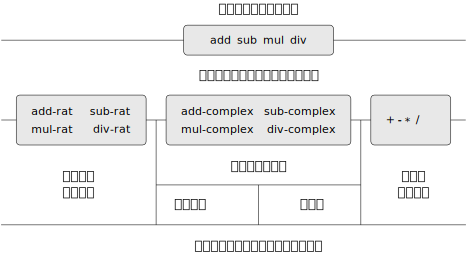
\includegraphics[width=111mm]{fig/chap2/Fig2.23a.pdf}
\par\bigskip
\noindent
\heading{Figure 2.23:} Generic arithmetic system.
\end{figure}

\noindent
\link{Figure 2.23} shows the structure of the system we shall build.  
Notice the
abstraction barriers.  From the perspective of someone using ``numbers,'' there
is a single procedure \code{add} that operates on whatever numbers are
supplied.  \code{Add} is part of a generic interface that allows the separate
ordinary-arithmetic, rational-arithmetic, and complex-arithmetic 
packages to be
accessed uniformly by programs that use numbers.  Any individual arithmetic
package (such as the complex package) may itself be accessed through generic
procedures (such as \code{add\-/complex}) that combine packages designed for
different representations (such as rectangular and polar).  Moreover, the
structure of the system is additive, so that one can design the individual
arithmetic packages separately and combine them to produce a generic arithmetic
system.

\link{Figure 2.23}は私達が構築するシステムの構造を示しています。
抽象化バリアに注目して下さい。``数値''を扱う第三者の視点からはそこにあるのは
どの種類の数値が提供されても単一の手続\code{add}です。\code{add}はジェネリックインターフェイスの
部分で別々の実数演算、分数演算、複素数演算のパッケージに、数値を使用するプログラムから統一的な
アクセスを可能にします。(複素数の様な)任意の個別数値演算パッケージはそれ自身が
(直行形式と極形式の様な)異なる表現のために設計されたパッケージを結合する
(\code{add\-/complex}の様な)ジェネリックな手続を通してアクセスできます。
さらに、システムの構造は付加的なため個々の数値演算パッケージは別々に設計することが可能で、
それらを結合してジェネリックな数値演算システムを生成できます。



\label{Section 2.5.1}
\subsection{Generic Arithmetic Operations}

The task of designing generic arithmetic operations is analogous to that of
designing the generic complex-number operations.  We would like, for instance,
to have a generic addition procedure \code{add} that acts like ordinary
primitive addition \code{+} on ordinary numbers, like \code{add\-/rat} on
rational numbers, and like \code{add\-/complex} on complex numbers.  We can
implement \code{add}, and the other generic arithmetic operations, by following
the same strategy we used in \link{Section 2.4.3} to implement the generic
selectors for complex numbers.  We will attach a type tag to each kind of
number and cause the generic procedure to dispatch to an appropriate package
according to the data type of its arguments.

ジェネリックな数値演算命令の設計タスクはジェネリックな複素数命令を設計するのと同様です。
例えば、実数上での通常の加算のプリミティブ\code{+}、分数上の\code{add\-/rat}や複素数上の
\code{add\-/complex}のように振る舞うジェネリックな加算手続\code{add}を持ちたいとします。
\code{add}と他のジェネリックな数値演算命令を\link{Section 2.4.3}にて複素数に対するジェネリックな
セレクタを実装するのに用いたのと同じ戦略に従うことで実装することが可能です。
全ての種類の数値にタイプタグをアタッチすることでジェネリック手続にその引数のデータタイプ
に従って適切なパッケージを呼び出す理由とします。

The generic arithmetic procedures are defined as follows:

ジェネリックな数値演算は以下のように定義されます。

\begin{scheme}
(define (add x y) (apply-generic 'add x y))
(define (sub x y) (apply-generic 'sub x y))
(define (mul x y) (apply-generic 'mul x y))
(define (div x y) (apply-generic 'div x y))
\end{scheme}

\noindent
We begin by installing a package for handling \newterm{ordinary} numbers, that
is, the primitive numbers of our language.  We will tag these with the symbol
\code{scheme\-/number}.  The arithmetic operations in this package are the
primitive arithmetic procedures (so there is no need to define extra procedures
to handle the untagged numbers).  Since these operations each take two
arguments, they are installed in the table keyed by the list
\code{(scheme\-/number scheme\-/number)}:

\newterm{ordinary}(通常の)数値を扱うためのパッケージをインストールすることで始めます。
これは私達の言語のプリミティブな数値のことです。これらにシンボル\code{scheme\-/number}で
タグを付けます。このパッケージ内の数値演算命令はプリミティブな数値演算手続です。
(そのためタグの無い数値を扱うために拡張手続を定義する必要はありません)。
これらの命令はそれぞれが2つの引数を取るためリスト\code{(scheme\-/number scheme\-/number)}を
鍵にしてテーブルにインストールされます。

\begin{scheme}
(define (install-scheme-number-package)
  (define (tag x) (attach-tag 'scheme-number x))
  (put 'add '(scheme-number scheme-number)
       (lambda (x y) (tag (+ x y))))
  (put 'sub '(scheme-number scheme-number)
       (lambda (x y) (tag (- x y))))
  (put 'mul '(scheme-number scheme-number)
       (lambda (x y) (tag (* x y))))
  (put 'div '(scheme-number scheme-number)
       (lambda (x y) (tag (/ x y))))
  (put 'make 'scheme-number (lambda (x) (tag x)))
  'done)
\end{scheme}

\noindent
Users of the Scheme-number package will create (tagged) ordinary numbers by
means of the procedure:

scheme-numberパッケージのユーザは(タグ付きの)普通の数値を手続を用いて作成します。

\begin{scheme}
(define (make-scheme-number n)
  ((get 'make 'scheme-number) n))
\end{scheme}

\noindent
Now that the framework of the generic arithmetic system is in place, we can
readily include new kinds of numbers.  Here is a package that performs rational
arithmetic.  Notice that, as a benefit of additivity, we can use without
modification the rational-number code from \link{Section 2.1.1} as the internal
procedures in the package:

さてこのジェネリック数値演算システムのフレームワークが準備できたので新しい種類の
数値も容易に含めることができます。ここに分数演算を実行するパッケージがあります。
付加的あることの利点として\link{Section 2.1.1}の分数コードをパッケージ内の内部手続として変更無しに
利用できることに注目して下さい。

\begin{scheme}
(define (install-rational-package)
  ~\textrm{;; internal procedures}~
  (define (numer x) (car x))
  (define (denom x) (cdr x))
  (define (make-rat n d)
    (let ((g (gcd n d)))
      (cons (/ n g) (/ d g))))
  (define (add-rat x y)
    (make-rat (+ (* (numer x) (denom y))
                 (* (numer y) (denom x)))
              (* (denom x) (denom y))))
  (define (sub-rat x y)
    (make-rat (- (* (numer x) (denom y))
                 (* (numer y) (denom x)))
              (* (denom x) (denom y))))
  (define (mul-rat x y)
    (make-rat (* (numer x) (numer y))
              (* (denom x) (denom y))))
  (define (div-rat x y)
    (make-rat (* (numer x) (denom y))
              (* (denom x) (numer y))))
  ~\textrm{;; interface to rest of the system}~
  (define (tag x) (attach-tag 'rational x))
  (put 'add '(rational rational)
       (lambda (x y) (tag (add-rat x y))))
  (put 'sub '(rational rational)
       (lambda (x y) (tag (sub-rat x y))))
  (put 'mul '(rational rational)
       (lambda (x y) (tag (mul-rat x y))))
  (put 'div '(rational rational)
       (lambda (x y) (tag (div-rat x y))))
  (put 'make 'rational
       (lambda (n d) (tag (make-rat n d))))
  'done)
(define (make-rational n d)
  ((get 'make 'rational) n d))
\end{scheme}

\noindent
We can install a similar package to handle complex numbers, using the tag
\code{complex}.  In creating the package, we extract from the table the
operations \code{make\-/from\-/real\-/imag} and \code{make\-/from\-/mag\-/ang} that were
defined by the rectangular and polar packages.  Additivity permits us to use,
as the internal operations, the same \code{add\-/complex}, \code{sub\-/complex},
\code{mul\-/complex}, and \code{div\-/complex} procedures from \link{Section 2.4.1}.

複素数を扱うために同様のパッケージをタグ\code{complex}を用いてインストールできます。
パッケージを作る際に、直行形式と極形式のパッケージにて定義された\code{make\-/from\-/real\-/imag}と
\code{make\-/from\-/mag\-/ang}の命令をテーブルから抽出します。付加性が内部命令として同じ
\link{Section 2.4.1}の手続\code{add\-/complex}, \code{sub\-/complex}, \code{mul\-/complex}, \code{div\-/complex}を
使用することを可能にします。

\begin{scheme}
(define (install-complex-package)
  ~\textrm{;; imported procedures from rectangular and polar packages}~
  (define (make-from-real-imag x y)
    ((get 'make-from-real-imag 'rectangular) x y))
  (define (make-from-mag-ang r a)
    ((get 'make-from-mag-ang 'polar) r a))
  ~\textrm{;; internal procedures}~
  (define (add-complex z1 z2)
    (make-from-real-imag (+ (real-part z1) (real-part z2))
                         (+ (imag-part z1) (imag-part z2))))
  (define (sub-complex z1 z2)
    (make-from-real-imag (- (real-part z1) (real-part z2))
                         (- (imag-part z1) (imag-part z2))))
  (define (mul-complex z1 z2)
    (make-from-mag-ang (* (magnitude z1) (magnitude z2))
                       (+ (angle z1) (angle z2))))
  (define (div-complex z1 z2)
    (make-from-mag-ang (/ (magnitude z1) (magnitude z2))
                       (- (angle z1) (angle z2))))
  ~\textrm{;; interface to rest of the system}~
  (define (tag z) (attach-tag 'complex z))
  (put 'add '(complex complex)
       (lambda (z1 z2) (tag (add-complex z1 z2))))
  (put 'sub '(complex complex)
       (lambda (z1 z2) (tag (sub-complex z1 z2))))
  (put 'mul '(complex complex)
       (lambda (z1 z2) (tag (mul-complex z1 z2))))
  (put 'div '(complex complex)
       (lambda (z1 z2) (tag (div-complex z1 z2))))
  (put 'make-from-real-imag 'complex
       (lambda (x y) (tag (make-from-real-imag x y))))
  (put 'make-from-mag-ang 'complex
       (lambda (r a) (tag (make-from-mag-ang r a))))
  'done)
\end{scheme}

\noindent
Programs outside the complex-number package can construct complex numbers
either from real and imaginary parts or from magnitudes and angles.  Notice how
the underlying procedures, originally defined in the rectangular and polar
packages, are exported to the complex package, and exported from there to the
outside world.

複素数パッケージの外側のプログラムは複素数を実数部と虚数部からでも大きさと角度からでも
構築することができます。元は直行形式と極形式のパッケージ内にて定義された内在する手続が
どのように複素数パッケージにエクスポートされているか、そしてそこからどのようにして
外部の世界へとエクスポートされているかについて注意して下さい。

\begin{scheme}
(define (make-complex-from-real-imag x y)
  ((get 'make-from-real-imag 'complex) x y))
(define (make-complex-from-mag-ang r a)
  ((get 'make-from-mag-ang 'complex) r a))
\end{scheme}

\noindent
What we have here is a two-level tag system.  A typical complex number, such as
\( 3 + 4i \) in rectangular form, would be represented as shown in \link{Figure 2.24}.  
The outer tag (\code{complex}) is used to direct the number to the
complex package.  Once within the complex package, the next tag
(\code{rectangular}) is used to direct the number to the rectangular package.
In a large and complicated system there might be many levels, each interfaced
with the next by means of generic operations.  As a data object is passed
``downward,'' the outer tag that is used to direct it to the appropriate
package is stripped off (by applying \code{contents}) and the next level of tag
(if any) becomes visible to be used for further dispatching.

ここで私達が行ったのは2つのレベルのタグシステムです。典型的な複素数、直交形式で
\( 3 + 4i \)のような物は\link{Figure 2.24}で示されるように表現されます。
外型のタグ(\code{complex})は数値を複素数パッケージへと導きます。複素数パッケージに入れば、
次のタグ(\code{rectangular})が数値を直行形式パッケージへと導きます。
巨大で複雑なシステムでは多くのレベルが存在するかもしれず、それぞれはジェネリックな命令を
用いて次へと接続されます。データオブジェクトが``下方''へ渡されるにつれ、適切なパッケージへ
導く外側のタグは(\code{contents}を適用することで)取り去られ、次のレベルのタグ(もし存在すれば)が
さらなる呼出のために使用されるため見えるようになります。

\begin{figure}[tb]
\phantomsection\label{Figure 2.24}
\centering
\begin{comment}
\heading{Figure 2.24:} Representation of \( 3 + 4i \) in rectangular form.

\begin{example}
     +---+---+     +---+---+     +---+---+
---->| * | *-+---->| * | *-+---->| * | * |
     +-|-+---+     +-|-+---+     +-|-+-|-+
       |             |             |   |
       V             V             V   V
 +---------+   +-------------+  +---+ +---+
 | complex |   | rectangular |  | 3 | | 4 |
 +---------+   +-------------+  +---+ +---+
\end{example}
\end{comment}
\includegraphics[width=64mm]{fig/chap2/Fig2.24c.pdf}
\begin{quote}
\heading{Figure 2.24:} Representation of \( 3 + 4i \) in rectangular form.
\end{quote}
\end{figure}

\noindent
In the above packages, we used \code{add\-/rat}, \code{add\-/complex}, and the
other arithmetic procedures exactly as originally written.  Once these
definitions are internal to different installation procedures, however, they no
longer need names that are distinct from each other: we could simply name them
\code{add}, \code{sub}, \code{mul}, and \code{div} in both packages.

上記のパッケージでは、\code{add\-/rat}, \code{add\-/complex}, それに他の数値演算手続を
全く元々書かれた状態で利用しました。しかし、これらの定義が異なるインストール手続の内部と
なれば直ぐに、お互いから識別可能である名前にする必要は無くなります。単純に両者のパッケージにて
\code{add}, \code{sub}, \code{mul}, \code{div}と名付けることが可能になります。

\begin{quote}
\heading{\phantomsection\label{Exercise 2.77}Exercise 2.77:} Louis Reasoner tries to evaluate
the expression \code{(magnitude z)} where \code{z} is the object shown in
\link{Figure 2.24}.  To his surprise, instead of the answer 5 he gets an error
message from \code{apply\-/generic}, saying there is no method for the operation
\code{magnitude} on the types \code{(complex)}.  He shows this interaction to
Alyssa P. Hacker, who says ``The problem is that the complex-number selectors
were never defined for \code{complex} numbers, just for \code{polar} and
\code{rectangular} numbers.  All you have to do to make this work is add the
following to the \code{complex} package:''

Louis Reasonerは\code{z}が\link{Figure 2.24}で示されるオブジェクトである場合に式
\code{(magnitude z)}を評価しようとした。驚いたことに、答の5の代わりに彼が受け取ったのは
\code{apply\-/generic}からのエラーメッセージで、型\code{(complex)}上に\code{magnitude}命令の
手段が存在しないと言う。彼はこの応答をAlyssa P. Hackerに見せた所、彼女は``問題は複素数セレクタが
\code{complex}の数値に対して定義されていない、\code{polar}と\code{rectangular}の数値に対してのみ
行われている。これを動かすためにしなければならないことは以下を\code{complex}パッケージに追加する
ことだ。''と述べた。

\begin{scheme}
(put 'real-part '(complex) real-part)
(put 'imag-part '(complex) imag-part)
(put 'magnitude '(complex) magnitude)
(put 'angle '(complex) angle)
\end{scheme}

Describe in detail why this works.  As an example, trace through all the
procedures called in evaluating the expression \code{(magnitude z)} where
\code{z} is the object shown in \link{Figure 2.24}.  In particular, how many
times is \code{apply\-/generic} invoked?  What procedure is dispatched to in each
case?

これでなぜ動くのか詳細を説明せよ。例として式\code{(magnitude z)}を\code{z}が\link{Figure 2.24}にて
示されるデータオブジェクトの場合に評価する時、呼び出される全ての手続をトレースせよ
具体的には、\code{apply\-/generic}は何回起動されるか? どの手続が各ケースに対して呼び出されるか?
\end{quote}

\begin{quote}
\heading{\phantomsection\label{Exercise 2.78}Exercise 2.78:} The internal procedures in the
\code{scheme\-/number} package are essentially nothing more than calls to the
primitive procedures \code{+}, \code{-}, etc.  It was not possible to use the
primitives of the language directly because our type-tag system requires that
each data object have a type attached to it.  In fact, however, all Lisp
implementations do have a type system, which they use internally.  Primitive
predicates such as \code{symbol?} and \code{number?}  determine whether data
objects have particular types.  Modify the definitions of \code{type\-/tag},
\code{contents}, and \code{attach\-/tag} from \link{Section 2.4.2} so that our
generic system takes advantage of Scheme's internal type system.  That is to
say, the system should work as before except that ordinary numbers should be
represented simply as Scheme numbers rather than as pairs whose \code{car} is
the symbol \code{scheme\-/number}.

\code{scheme\-/number}パッケージの内部手続は本質的にプリミティブな手続\code{+}, \code{-}, その他の
呼出し以上の物ではない。言語のプリミティブを直接使用することはできない。
私達のタイプタグシステムが各データオブジェクトに対し型付けられていることを要件とするため
である。しかし実際には全てのLisp実装は型システムを持っており、内部にて使用している。
\code{symbol?}や\code{number?}のようなプリミティブな述語はデータオブジェクトが特定の型を持つか
決定する。\link{Section 2.4.2}の\code{type\-/tag}, \code{contents}, and \code{attach\-/tag}の定義を変更し
私達のジェネリックシステムがSchemeの内部型システムの利点を得るようにせよ。
これは言い替えれば、
システムは以前と同じように動作する必要があるが、ただし普通の数値はその\code{car}がシンボル
\code{scheme\-/number}であるペアでなく、単純にSchemeの数値として表現されるようにせよ。
\end{quote}

\begin{quote}
\heading{\phantomsection\label{Exercise 2.79}Exercise 2.79:} Define a generic equality
predicate \code{equ?} that tests the equality of two numbers, and install it in
the generic arithmetic package.  This operation should work for ordinary
numbers, rational numbers, and complex numbers.

2つの数値の等値関係をテストするジェネリックな等値の述語\code{equ?}を定義し、
ジェネリック数値演算パッケージにインストールせよ。この命令は通常の数値、分数、
複素数に対しても働くこと。
\end{quote}

\begin{quote}
\heading{\phantomsection\label{Exercise 2.80}Exercise 2.80:} Define a generic predicate
\code{=zero?} that tests if its argument is zero, and install it in the generic
arithmetic package.  This operation should work for ordinary numbers, rational
numbers, and complex numbers.

引数が0であるかテストするジェネリックな述語\code{=zero?}を定義しジェネリック数値
演算パッケージにインストールせよ。この命令は通常の数値、分数、
複素数に対しても働くこと。
\end{quote}

\label{Section 2.5.2}
\subsection{Combining Data of Different Types}

We have seen how to define a unified arithmetic system that encompasses
ordinary numbers, complex numbers, rational numbers, and any other type of
number we might decide to invent, but we have ignored an important issue.  The
operations we have defined so far treat the different data types as being
completely independent.  Thus, there are separate packages for adding, say, two
ordinary numbers, or two complex numbers.  What we have not yet considered is
the fact that it is meaningful to define operations that cross the type
boundaries, such as the addition of a complex number to an ordinary number.  We
have gone to great pains to introduce barriers between parts of our programs so
that they can be developed and understood separately.  We would like to
introduce the cross-type operations in some carefully controlled way, so that
we can support them without seriously violating our module boundaries.

通常の数値、複素数、分数、そして開発するだろう任意の他の型の数値を包括する
統一数値演算システムをどのように定義するかについて学びました。しかし私達は
重要な問題を無視してきました。今まで私達が定義した命令は異なるデータの型を
完全に独立しているとして扱ってきました。従って追加すべき分かれたパッケージが、
例えば2つの普通の数値や2つの複素数が存在します。私達がまだ考慮していないことは
型の境界を渡る命令を定義することには意義があるという事実です。例えば複素数と実数の
加算です。私達はこれまでプログラムの間にバリアを築くために大きな努力をしてきました。
それが分離して開発、理解されることを可能にするためでした。私達は型を渡る命令を
ある程度注意深くコントロールされた手段にて導入したいと思います。そうすることで
私達のモジュール境界を重大な侵害が起こらないようにそれらをサポートすることがで
きるようにです。

One way to handle cross-type operations is to design a different procedure for
each possible combination of types for which the operation is valid.  For
example, we could extend the complex-number package so that it provides a
procedure for adding complex numbers to ordinary numbers and installs this in
the table using the tag \code{(complex scheme\-/number)}:\footnote{We also have
to supply an almost identical procedure to handle the types
\code{(scheme\-/number complex)}.}

クロスタイプ(型を渡る)命令を扱う1つの方法は命令が有効な型の可能な組み合わせそれぞれに
対して異なる手続を設計することです。例えば複素数パッケージを拡張し、それが複素数と実数
の加算を提供し、タグ\code{(complex scheme\-/number)}を用いてテーブルにインストールするように
します。\footnote{私達はまたほとんど同一の手続を型\code{(scheme\-/number complex)}を扱うために
提供しなければなりません。}

\begin{scheme}
~\textrm{;; to be included in the complex package}~
(define (add-complex-to-schemenum z x)
  (make-from-real-imag (+ (real-part z) x) (imag-part z)))
(put 'add '(complex scheme-number)
     (lambda (z x) (tag (add-complex-to-schemenum z x))))
\end{scheme}

\noindent
This technique works, but it is cumbersome.  With such a system, the cost of
introducing a new type is not just the construction of the package of
procedures for that type but also the construction and installation of the
procedures that implement the cross-type operations.  This can easily be much
more code than is needed to define the operations on the type itself.  The
method also undermines our ability to combine separate packages additively, or
at least to limit the extent to which the implementors of the individual packages
need to take account of other packages.  For instance, in the example above, it
seems reasonable that handling mixed operations on complex numbers and ordinary
numbers should be the responsibility of the complex-number package.  Combining
rational numbers and complex numbers, however, might be done by the complex
package, by the rational package, or by some third package that uses operations
extracted from these two packages.  Formulating coherent policies on the
division of responsibility among packages can be an overwhelming task in
designing systems with many packages and many cross-type operations.

このテクニックはうまく行きますが、面倒です。このようなシステムでは新しい型を導入する
コストはその型のための手続のパッケージを構築するだけでなく、クロスタイプの命令を
実装する手続の構築とインストールに及びます。これは簡単にその型自身の命令を定義するため
に必要なものよりより多くのコードとなるでしょう。この手法はまた分かれたパッケージを付加的に接続する
能力を弱めたり、最低でも個々のパッケージの実装者が他のパッケージの考慮をしなければなら
ない範囲を制約する能力をダメにしてしまいます。
例えば、上の例では複素数と実数上の混合命令の扱いが複素数パッケージの責任となるのは
妥当に見えます。しかし分数と複素数の接続においては複素数パッケージで行われるかもしれないし、
分数パッケージかもしれないし、これらの2つのパッケージから抽出した命令を用いる
何らかの第三者パッケージかもしれません。パッケージ間の区分上における整合性のポリシー
の形式化が、多くのパッケージと多くのクロスタイプ命令を伴なうシステム設計において
計り知れなくなってしまいます。

\subsubsection*{Coercion}

In the general situation of completely unrelated operations acting on
completely unrelated types, implementing explicit cross-type operations,
cumbersome though it may be, is the best that one can hope for.  Fortunately,
we can usually do better by taking advantage of additional structure that may
be latent in our type system.  Often the different data types are not
completely independent, and there may be ways by which objects of one type may
be viewed as being of another type.  This process is called \newterm{coercion}.
For example, if we are asked to arithmetically combine an ordinary number with
a complex number, we can view the ordinary number as a complex number whose
imaginary part is zero.  This transforms the problem to that of combining two
complex numbers, which can be handled in the ordinary way by the
complex-arithmetic package.

完全に依存しない型達上にて振る舞う完全に依存しない命令群が一般的な状況においては
明示的にクロスタイプ命令を実装することは、面倒かもしれませんが、人が望む最高の
物かもしれません。幸運なことに私達は通常、私達の型システム内の潜在的に存在する
だろう付加的な構造の利点を用いることによりより良く行うことが可能です。
時折、異なるデータの型は完全には独立しておらず、ある型のオブジェクトが
他の型であるように見られる場合が複数存在するでしょう。
この過程は\newterm{coercion}(強制)と呼ばれます。例えばもし私達が算術上、
実数と複素数を合成するよう求められた場合に、私達は実数を虚数部が0の複素数だと
見做すことができます。これはこの問題を2つの複素数の合成へと変換し、複素数パッケージ
により通常の方法にて取り扱うことが可能になります。

In general, we can implement this idea by designing coercion procedures that
transform an object of one type into an equivalent object of another type.
Here is a typical coercion procedure, which transforms a given ordinary number
to a complex number with that real part and zero imaginary part:

一般的に、ある型のオブジェクトを等価な他の型のオブジェクトに変換する強制手続を
設計することでこの考えを実装することができます。以下は典型的な強制手続です。
これは与えられた普通の数値(実数)を実数部とゼロである虚数部を持つ複素数に変換します。

\begin{scheme}
(define (scheme-number->complex n)
  (make-complex-from-real-imag (contents n) 0))
\end{scheme}

\noindent
We install these coercion procedures in a special coercion table, indexed under
the names of the two types:

これらの強制手続を2つの型の名前により索引付けした特別な強制テーブルにインストールします。

\begin{scheme}
(put-coercion 'scheme-number
              'complex 
              scheme-number->complex)
\end{scheme}

\noindent
(We assume that there are \code{put\-/coercion} and \code{get\-/coercion}
procedures available for manipulating this table.)  Generally some of the slots
in the table will be empty, because it is not generally possible to coerce an
arbitrary data object of each type into all other types.  For example, there is
no way to coerce an arbitrary complex number to an ordinary number, so there
will be no general \code{complex\-/>scheme\-/number} procedure included in the
table.

(このテーブルを操作するために手続\code{put\-/coercion}と\code{get\-/coercion}が存在すると仮定します)。
一般にこのテーブルの枠のいくつかは空になります。全ての型の任意のデータオブジェクトを全ての
他の型へと強制することは一般には不可能です。例えば任意の複素数を実数に強制することはできません。
そのため普遍的な\code{complex\-/>scheme\-/number}手続はテーブルに含まれることはありません。

Once the coercion table has been set up, we can handle coercion in a uniform
manner by modifying the \code{apply\-/generic} procedure of \link{Section 2.4.3}.
When asked to apply an operation, we first check whether the operation is
defined for the arguments' types, just as before.  If so, we dispatch to the
procedure found in the operation-and-type table.  Otherwise, we try coercion.
For simplicity, we consider only the case where there are two
arguments.\footnote{See \link{Exercise 2.82} for generalizations.}  We check the
coercion table to see if objects of the first type can be coerced to the second
type.  If so, we coerce the first argument and try the operation again.  If
objects of the first type cannot in general be coerced to the second type, we
try the coercion the other way around to see if there is a way to coerce the
second argument to the type of the first argument.  Finally, if there is no
known way to coerce either type to the other type, we give up.  Here is the
procedure:

強制テーブルが準備されれば、\link{Section 2.4.3}の\code{apply\-/generic}手続を変更することで
統一的な作法で強制を取り扱うことができます。命令を適用するよう求められた時、
最初にその命令が引数の型に対して定義されているかどうかを以前と同様にチェックします。
もしそうであれば命令と型のテーブルで見つかった手続を呼び出します。そうでなければ
強制を試みます。単純化のために、2つの引数を伴う場合のみについて考えることにします。\footnote{
一般化については\link{Exercise 2.82}を参照して下さい。}
強制テーブルをチェックし、最初の型のオブジェクトが2つ目の型に強制できるか確認します。
もしそうであれば、最初の引数を強制し、命令の試行を再び行います。もし最初の型のオブジェクトが
一般に2つ目の型に強制できない場合、逆に2つ目の引数を1つ目の引数の型に強制できるか試します。
最後にどちらの型も他方の型に強制できない場合、諦めます。以下がこの手続です。

\begin{smallscheme}
(define (apply-generic op . args)
  (let ((type-tags (map type-tag args)))
    (let ((proc (get op type-tags)))
      (if proc
          (apply proc (map contents args))
          (if (= (length args) 2)
              (let ((type1 (car type-tags))
                    (type2 (cadr type-tags))
                    (a1 (car args))
                    (a2 (cadr args)))
                (let ((t1->t2 (get-coercion type1 type2))
                      (t2->t1 (get-coercion type2 type1)))
                  (cond (t1->t2 
                         (apply-generic op (t1->t2 a1) a2))
                        (t2->t1 
                         (apply-generic op a1 (t2->t1 a2)))
                        (else (error "No method for these types"
                                     (list op type-tags))))))
              (error "No method for these types"
                     (list op type-tags)))))))
\end{smallscheme}

\noindent
This coercion scheme has many advantages over the method of defining explicit
cross-type operations, as outlined above.  Although we still need to write
coercion procedures to relate the types (possibly \( n^2 \) procedures for a
system with \( n \) types), we need to write only one procedure for each pair of
types rather than a different procedure for each collection of types and each
generic operation.\footnote{If we are clever, we can usually get by with fewer
than \( n^2 \) coercion procedures.  For instance, if we know how to convert from
type 1 to type 2 and from type 2 to type 3, then we can use this knowledge to
convert from type 1 to type 3.  This can greatly decrease the number of
coercion procedures we need to supply explicitly when we add a new type to the
system.  If we are willing to build the required amount of sophistication into
our system, we can have it search the ``graph'' of relations among types and
automatically generate those coercion procedures that can be inferred from the
ones that are supplied explicitly.}  What we are counting on here is the fact
that the appropriate transformation between types depends only on the types
themselves, not on the operation to be applied.

この強制スキームは上で概説された様に明示的なクロスタイプ命令の定義手法上に多くの利点を持ちます。
私達は依然、型に関係する強制手続を書かねばなりませんが(\( n \)個の型のシステムに対し
場合により\( n^2 \)の手続)、全ての型の集合と各ジェネリック命令に対し異なる手続を書くのでなく、
型のペア1組につき1つの手続を書くだけで済みます。\footnote{
もし私達が賢いならば普通は\( n^2 \)よりも少ない強制手続で済みます。例えばもし型1から型2
への変換方法と型2から型3への変換方法を知っている場合、この知識を用いて型1から型3へ変換することが
できます。これはシステムに新しい型を追加する時に明示的に提供せねばならない強制手続の数を
劇的に減らします。もしシステムに必要なだけの洗練を組み入れたいのなら、システムにタイプ間の
``グラフ''を検索させて自動的に明示的に提供された物から推論可能な強制手続を生成させることが可能です。}
ここで私達が信頼しているものはタイプ間の適切な変換は型それ自身のみに依存し、適用される命令には
依存しないという事実です。

On the other hand, there may be applications for which our coercion scheme is
not general enough.  Even when neither of the objects to be combined can be
converted to the type of the other it may still be possible to perform the
operation by converting both objects to a third type.  In order to deal with
such complexity and still preserve modularity in our programs, it is usually
necessary to build systems that take advantage of still further structure in
the relations among types, as we discuss next.

一方で、私達の強制スキームが十分に汎用ではないアプリケーションが存在するかもしれません。
たとえ合成されるオブジェクトの両方ともが他方に変換できないとしても両者を第三の型に
変換することで命令を実行することが可能になるかもしれません。そのような複雑さに対処する
ため、そしてそれでもプログラムのモジュール方式を維持するために、通常はより一層タイプ間の
関係の構造の利点を得るシステムを構築することが、次で議論するように必要です。

\subsubsection*{Hierarchies of types}

The coercion scheme presented above relied on the existence of natural
relations between pairs of types.  Often there is more ``global'' structure in
how the different types relate to each other.  For instance, suppose we are
building a generic arithmetic system to handle integers, rational numbers, real
numbers, and complex numbers.  In such a system, it is quite natural to regard
an integer as a special kind of rational number, which is in turn a special
kind of real number, which is in turn a special kind of complex number.  What
we actually have is a so-called \newterm{hierarchy of types}, in which, for
example, integers are a \newterm{subtype} of rational numbers (i.e., any
operation that can be applied to a rational number can automatically be applied
to an integer).  Conversely, we say that rational numbers form a
\newterm{supertype} of integers.  The particular hierarchy we have here is of a
very simple kind, in which each type has at most one supertype and at most one
subtype.  Such a structure, called a \newterm{tower}, is illustrated in
\link{Figure 2.25}.

上で展開された強制スキームは型のペアの間の自然な関係の存在に当てにしていました。
より``一般的な''構造が、異なる型のお互いへの関係の仕方には良く存在します。
例えば、私達が整数、分数、実数、複素数を扱う一般的な数値演算システムを構築していると
仮定します。そのようなシステムにおいては整数を特別な種類の分数として見做すことは
とても自然です。分数は同様に特別な種類の実数であり、実数は同様に特別な種類の
複素数であります。私達が実際に手にしている物は\newterm{hierarchy of types}(型の階層)
呼ばれるもので、その中では例えば整数は分数の\newterm{subtype}(サブタイプ)です(すなわち
分数に適用できる任意の命令は自動的に整数に適用できます)。逆に分数は整数の
\newterm{supertype}(スーパータイプ、親の型)と呼びます。今手にした階層はとても単純な
種類で、各型はたかだか1つのスーパータイプを持ち、たかだか1つのサブタイプを持ちます。
そのような構造は\newterm{tower}(タワー、塔)と呼ばれ\link{Figure 2.25}で示されます。

\begin{figure}[tb]
\phantomsection\label{Figure 2.25}
\centering
\begin{comment}
\heading{Figure 2.25:} A tower of types.

\begin{example}
 complex
   ^
   |
  real
   ^
   |
rational
   ^
   |
integer
\end{example}
\end{comment}
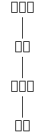
\includegraphics[width=11mm]{fig/chap2/Fig2.25.pdf}
\par\bigskip
\noindent
\heading{Figure 2.25:} A tower of types.
\end{figure}

\noindent
If we have a tower structure, then we can greatly simplify the problem of
adding a new type to the hierarchy, for we need only specify how the new type
is embedded in the next supertype above it and how it is the supertype of the
type below it.  For example, if we want to add an integer to a complex number,
we need not explicitly define a special coercion procedure
\code{integer\-/>complex}.  Instead, we define how an integer can be transformed
into a rational number, how a rational number is transformed into a real
number, and how a real number is transformed into a complex number.  We then
allow the system to transform the integer into a complex number through these
steps and then add the two complex numbers.

もしタワー構造を持つ場合、階層に新しい型を追加する問題を著しく単純化できます。
新しい型がどのようにその上のスーパータイプの隣に組込まれるか、そしてどのように
その型がその下の型に対してスーパータイプであるかを指定するだけです。
例えばもし複素数に対して整数を追加したい場合、明示的に特別な強制手続
\code{integer\-/>complex}を定義する必要はありません。その代わりに整数がどのように分数に
変換できるか、分数がどのように実数に変換できるか、実数がどのように複素数に変換でき
るかを定義します。そうしたらシステムに整数を複素数に変換することをこれらのステップ
を通して変換することを許可し、次に2つの複素数を加算します。

We can redesign our \code{apply\-/generic} procedure in the following way: For
each type, we need to supply a \code{raise} procedure, which ``raises'' objects
of that type one level in the tower.  Then when the system is required to
operate on objects of different types it can successively raise the lower types
until all the objects are at the same level in the tower.  (\link{Exercise 2.83}
and \link{Exercise 2.84} concern the details of implementing such a strategy.)

\code{apply\-/generic}手続を以下のように再設計することもできます。各型に対して
\code{raise}手続を与える必要があります。これはある型のオブジェクトをタワーにおいて
1レベル上げます。そうすればシステムが異なる型のオブジェクト上にて操作する必要がある時、
全てのオブジェクトがタワー内にて同じレベルになるまで連続して上げることができます
(\link{Exercise 2.83}と\link{Exercise 2.84}がそのような戦略の実装の詳細について
考察しています)。

Another advantage of a tower is that we can easily implement the notion that
every type ``inherits'' all operations defined on a supertype.  For instance,
if we do not supply a special procedure for finding the real part of an
integer, we should nevertheless expect that \code{real\-/part} will be defined
for integers by virtue of the fact that integers are a subtype of complex
numbers.  In a tower, we can arrange for this to happen in a uniform way by
modifying \code{apply\-/generic}.  If the required operation is not directly
defined for the type of the object given, we raise the object to its supertype
and try again.  We thus crawl up the tower, transforming our argument as we go,
until we either find a level at which the desired operation can be performed or
hit the top (in which case we give up).

タワーの別の利点には全ての型がスーパータイプ上に定義された全ての命令を``継承''する
概念を簡単に実装できることが上げられます。例えばもし整数の実数部を求めるための
特別な手続を提供しない場合、それにもかかわらず
整数は複素数のサブタイプであるという事実のおかげで、整数のための\code{real\-/part}が
定義されることが期待できます。タワーでは\code{apply\-/generic}を変更するという統一的な
方法でこの様なことが起こるよう準備することが可能です。
もし必要な命令が与えられたオブジェクトの型のために直接定義されていない場合、
オブジェクトをそのスーパータイプに上げることで再試行できます。従ってタワーを
這い上がりながら望まれた命令が実行可能になるまで引数を変換するか、頂上まで辿り
ついてそこで諦めることができます。

Yet another advantage of a tower over a more general hierarchy is that it gives
us a simple way to ``lower'' a data object to the simplest representation.  For
example, if we add \( 2 + 3i \) to \( 4 - 3i \), it would be nice to obtain the
answer as the integer 6 rather than as the complex number \( 6 + 0i \).
\link{Exercise 2.85} discusses a way to implement such a lowering operation.
(The trick is that we need a general way to distinguish those objects that can
be lowered, such as \( 6 + 0i \), from those that cannot, such as \( 6 + 2i \).)

別のより一般的な階層に比べた場合、もう1つタワーの利点はデータオブジェクトをより簡単な
表現へ``下げる''簡単な方法を提供することです。例えば\( 2 + 3i \)を\( 4 - 3i \)に
足した場合、その答は複素数\( 6 + 0i \)よりも整数6で得るほうがより良いと言えるでしょう。
\link{Exercise 2.85}はそのようなレベルを下げる命令の実装について議論します。
(この仕掛けには\( 6 + 0i \)のような階層のレベルを下げられるオブジェクトを
\( 6 + 2i \)のような下げられないオブジェクトから見分ける一般的な方法が必要です)。

\subsubsection*{Inadequacies of hierarchies}

If the data types in our system can be naturally arranged in a tower, this
greatly simplifies the problems of dealing with generic operations on different
types, as we have seen.  Unfortunately, this is usually not the case.
\link{Figure 2.26} illustrates a more complex arrangement of mixed types, this
one showing relations among different types of geometric figures.  We see that,
in general, a type may have more than one subtype.  Triangles and
quadrilaterals, for instance, are both subtypes of polygons.  In addition, a
type may have more than one supertype.  For example, an isosceles right
triangle may be regarded either as an isosceles triangle or as a right
triangle.  This multiple-supertypes issue is particularly thorny, since it
means that there is no unique way to ``raise'' a type in the hierarchy.
Finding the ``correct'' supertype in which to apply an operation to an object
may involve considerable searching through the entire type network on the part
of a procedure such as \code{apply\-/generic}.  Since there generally are
multiple subtypes for a type, there is a similar problem in coercing a value
``down'' the type hierarchy.  Dealing with large numbers of interrelated types
while still preserving modularity in the design of large systems is very
difficult, and is an area of much current research.\footnote{This statement,
which also appears in the first edition of this book, is just as true now as it
was when we wrote it twelve years ago.  Developing a useful, general framework
for expressing the relations among different types of entities (what
philosophers call ``ontology'') seems intractably difficult.  The main
difference between the confusion that existed ten years ago and the confusion
that exists now is that now a variety of inadequate ontological theories have
been embodied in a plethora of correspondingly inadequate programming
languages.  For example, much of the complexity of object-oriented programming
languages---and the subtle and confusing differences among contemporary
object-oriented languages---centers on the treatment of generic operations on
interrelated types.  Our own discussion of computational objects in
\link{Chapter 3} avoids these issues entirely.  Readers familiar with
object-oriented programming will notice that we have much to say in
chapter 3 about local state, but we do not even mention ``classes'' or
``inheritance.''  In fact, we suspect that these problems cannot be adequately
addressed in terms of computer-language design alone, without also drawing on
work in knowledge representation and automated reasoning.}

もしシステムのデータの型が自然にタワーに配置できる場合、ここまで見てきた通りに、
異なる型上のジェネリック命令の取扱の問題を著しく単純化できます。
残念なことに、これは普通の場合ではありません。\link{Figure 2.26} は雑多な型のより複雑な
配置を図示しています。この図は幾何学的図形の異なる型の間の関係を見せています。
一般的に1つの型が複数のサブタイプを持つことがわかります。例えば三角形と四角形は
共に多角形のサブタイプです。加えてある型は複数のスーパータイプを持つことがあり得ます。
例えば二等辺直角三角形は二等辺三角形、または直角三角形と見做すことができます。
この複数スーパータイプ問題は特に困難で、階層内において型を``上げる''単一の方法が
存在しません。オブジェクトに命令を適用するため``正しい''スーパータイプを求めることは
\code{apply\-/generic}の様な手続に不可欠な型ネットワーク全体を通しての多大な検索を巻き起す
可能性があります。一般的にある型に対して複数のサブタイプが存在するので値に対し型階層を
``下げる''強制にも同様の問題が存在します。巨大システムの設計におけるモジュール化方式を
それでも維持しながら多くの数の相互に関係する型の取り扱うことはとても難しく、現在の多くの
研究領域です。\footnote{
第一版でも存在したこの文は12年前と同じく今も変わりません。実用的で汎用的な異なる型の
要素間の関係の表現するフレームワーク(哲学者が``オントロジー''(存在論)と呼ぶもの)を
開発することは不可能に見えるほど難しいことです。10年前に存在した混乱と現在に存在する混乱との間の
違いは、種々の不適切な存在論上の理論が、相応して不適切なプログラミング言語に過剰に組込まれてい
ることです。例えばオブジェクト指向言語の複雑性の多くは---そして現在のオブジェクト指向言語間の
微妙で混乱させる違いは---相互に関係する型上のジェネリック命令の扱いを中心とします。
\link{Chapter 3}での私達自身による計算オブジェクトの議論はこれらの問題を完全に避けます。
オブジェクト指向言語に親しみのある読者は\link{Chapter 3}においてローカルの状態について多くの
触れるべきことが存在すると気付くでしょう。しかし私達は``クラス''や``継承''についてさえ
述べることはしません。実際に私達はこれらの問題が知識表現上の成果の利用と自動的な推論無しに
コンピュータ言語設計のみで適切に解決されることは無いと疑っています。}

\begin{figure}[tb]
\phantomsection\label{Figure 2.26}
\centering
\begin{comment}
\heading{Figure 2.26:} Relations among types of geometric figures.

\begin{example}
                     polygon
                    /       \
                   /         \
            triangle         quadrilateral
            /     \              /     \
           /       \            /       \
     isosceles   right      trapezoid   kite
     triangle    triangle       |         |
      |     \      |            |         |
      |      \     |            |         |
equilateral   isosceles   parallelogram   |
triangle      right          |       \    |
              triangle       |        \   |
                          rectangle  rhombus
                                \    /
                                 \  /
                                square
\end{example}
\end{comment}
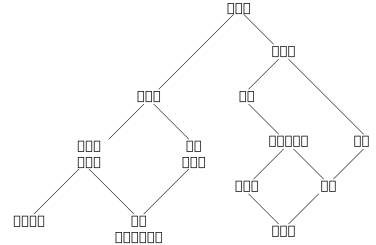
\includegraphics[width=96mm]{fig/chap2/Fig2.26e.pdf}
\par\bigskip
\noindent
\heading{Figure 2.26:} Relations among types of geometric figures.
\end{figure}

\begin{quote}
\heading{\phantomsection\label{Exercise 2.81}Exercise 2.81:} Louis Reasoner has noticed that
\code{apply\-/generic} may try to coerce the arguments to each other's type even
if they already have the same type.  Therefore, he reasons, we need to put
procedures in the coercion table to \newterm{coerce} arguments of each type to
their own type.  For example, in addition to the
\code{scheme\-/number\-/>complex} coercion shown above, he would do:

Louis Reasonerは\code{apply\-/generic}が引数に対しそれらが既に同じ型であってもお互いの
型に強制を試行することに気付いた。そのため彼は強制テーブルに各型の引数をそれら自身の
型に\newterm{coerce}(強制)するための手続を追加する必要があるのではないかと``reason''(推論)
した。

\begin{scheme}
(define (scheme-number->scheme-number n) n)
(define (complex->complex z) z)
(put-coercion 'scheme-number 
              'scheme-number
              scheme-number->scheme-number)
(put-coercion 'complex 'complex complex->complex)
\end{scheme}

\begin{enumerate}[a]

\item
With Louis's coercion procedures installed, what happens if
\code{apply\-/generic} is called with two arguments of type \code{scheme\-/number}
or two arguments of type \code{complex} for an operation that is not found in
the table for those types?  For example, assume that we've defined a generic
exponentiation operation:

Louisの強制手続がインストールされると\code{apply\-/generic}が命令に対する
2つの引数の型が\code{scheme\-/number}、または2つの引数の型が\code{complex}であり
それらの型に対する命令がテーブルに存在しない場合何が起こるだろうか?
例えばジェネリックな指数関数命令を定義したとしよう。

\begin{scheme}
(define (exp x y) (apply-generic 'exp x y))
\end{scheme}

\noindent
and have put a procedure for exponentiation in the Scheme-number
package but not in any other package:

そしてScheme-numberパッケージの指数関数に対する手続を追加したとする。
ただし他の型に関しては全て行わない。

\begin{scheme}
~\textrm{;; following added to Scheme-number package}~
(put 'exp '(scheme-number scheme-number)
     (lambda (x y) (tag (expt x y)))) 
     ~\textrm{; using primitive \code{expt}}~
\end{scheme}

\noindent
What happens if we call \code{exp} with two complex numbers as arguments?

2つの複素数引数により\code{exp}を呼び出した場合、何が起こるだろうか?

\item
Is Louis correct that something had to be done about coercion with arguments of
the same type, or does \code{apply\-/generic} work correctly as is?

同じ型の引数に伴なう強制に関して何かが行われるべきかについてLouisは正しいだろうか?
それとも\code{apply\-/generic}はそのままで正しく動作するだろうか?

\item
Modify \code{apply\-/generic} so that it doesn't try coercion if the two
arguments have the same type.

\code{apply\-/generic}を変更し2つの引数が同じ型である場合に強制を試行しないようにせよ。

\end{enumerate}
\end{quote}

\begin{quote}
\heading{\phantomsection\label{Exercise 2.82}Exercise 2.82:} Show how to generalize
\code{apply\-/generic} to handle coercion in the general case of multiple
arguments.  One strategy is to attempt to coerce all the arguments to the type
of the first argument, then to the type of the second argument, and so on.
Give an example of a situation where this strategy (and likewise the
two-argument version given above) is not sufficiently general.  (Hint: Consider
the case where there are some suitable mixed-type operations present in the
table that will not be tried.)

\code{apply\-/generic}を複数引数の全体的な場合に強制を扱わせるような一般化を行わせるには
どのように行うかを示せ。1つの戦略として全ての引数を最初の引数の型に強制するよう
試行し、次に2つ目、以降繰り返しが上げられる。この戦略(と上で与えられた2引数版が
同様に)全体には不十分である例を示せ。(ヒント:テーブルにいくつか適切な型が混ざった
命令が存在し、それが試行されない場合について考えよ。)
\end{quote}

\begin{quote}
\heading{\phantomsection\label{Exercise 2.83}Exercise 2.83:} Suppose you are designing a
generic arithmetic system for dealing with the tower of types shown in
\link{Figure 2.25}: integer, rational, real, complex.  For each type (except
complex), design a procedure that raises objects of that type one level in the
tower.  Show how to install a generic \code{raise} operation that will work for
each type (except complex).

\link{Figure 2.25}で示される型のタワーを取り扱うジェネリックな数値演算システムの
設計を行っているとする。整数、分数、実数、複素数に対応する。各型(複素数を除く)に
対してその型のオブジェクトをタワー内にて1レベル上げる手続を設計せよ。
(複素数を除く)各型に対し動作するジェネリックな\code{raise}命令をどのようにインストールするか
示せ。
\end{quote}

\begin{quote}
\heading{\phantomsection\label{Exercise 2.84}Exercise 2.84:} Using the \code{raise} operation
of \link{Exercise 2.83}, modify the \code{apply\-/generic} procedure so that it
coerces its arguments to have the same type by the method of successive
raising, as discussed in this section.  You will need to devise a way to test
which of two types is higher in the tower.  Do this in a manner that is
``compatible'' with the rest of the system and will not lead to problems in
adding new levels to the tower.

\link{Exercise 2.83}の\code{raise}命令を用いて\code{apply\-/generic}手続を変更し、
複数の引数が一連の``上げる''動作を行うことによりこの節で語られた様に同じ型を持つようにせよ。
2つの型のどちらがタワー内にてより高いレベルであるかテストする手段を開発する必要がある。
これを残りのシステムと``互換性''を保ち、タワーに新しいレベルを追加する場合にも
問題が無いような手段で行え。
\end{quote}

\begin{quote}
\heading{\phantomsection\label{Exercise 2.85}Exercise 2.85:} This section mentioned a method
for ``simplifying'' a data object by lowering it in the tower of types as far
as possible.  Design a procedure \code{drop} that accomplishes this for the
tower described in \link{Exercise 2.83}.  The key is to decide, in some general
way, whether an object can be lowered.  For example, the complex number 
\( 1.5 + 0i \) can be lowered as far as \code{real}, the complex number \( 1 + 0i \) can
be lowered as far as \code{integer}, and the complex number \( 2 + 3i \) cannot
be lowered at all.  Here is a plan for determining whether an object can be
lowered: Begin by defining a generic operation \code{project} that ``pushes''
an object down in the tower.  For example, projecting a complex number would
involve throwing away the imaginary part.  Then a number can be dropped if,
when we \code{project} it and \code{raise} the result back to the type we
started with, we end up with something equal to what we started with.  Show how
to implement this idea in detail, by writing a \code{drop} procedure that drops
an object as far as possible.  You will need to design the various projection
operations\footnote{A real number can be projected to an integer using the
\code{round} primitive, which returns the closest integer to its argument.} and
install \code{project} as a generic operation in the system.  You will also
need to make use of a generic equality predicate, such as described in
\link{Exercise 2.79}.  Finally, use \code{drop} to rewrite \code{apply\-/generic}
from \link{Exercise 2.84} so that it ``simplifies'' its answers.

この節では可能な限りタワー内の型レベルを下げることによりデータオブジェクトの``単純化''を
行う手段について説明した。\link{Exercise 2.83}に記述されたタワーに対しこれを達成する手続\code{drop}
を設計せよ。いくつかの一般的な方法の中から決定する鍵は、オブジェクトを下げることができるか
どうかである。例えば複素数\( 1.5 + 0i \)は\code{real}(実数)である限り下げられ、複素数\( 1 + 0i \)
は\code{integer}(整数)である限り下げることができ、複素数\( 2 + 3i \)は下げることが絶対にできない。
以下に、あるオブジェクトが下げることができるか決定する計画を示す。
オブジェクトをタワー内にて``押し下げる''ジェネリックな命令\code{project}(射影)を定義することから始める。
例えば複素数の射影は虚数部を捨てることになる。すると数値は\code{project}した結果を
元の型に\code{raise}(上げ)た時に開始した時点と同じ値になれば\code{drop}(落とす)ことができる
ことになる。可能な場合にオブジェクトを落とす手続\code{drop}を書くことで、この考えをどのように実装するか
詳細に示せ。色々な射影命令を設計し、ジェネリックな命令として\code{project}をシステム内にインストール
する必要がある。\footnote{
実数は引数に最も近い整数を返すプリミティブ\code{round}を用いて整数に射影することができる。}
また\link{Exercise 2.79}で説明した等値関係のジェネリックな述語を利用する必要もある。
最後に\code{drop}を用いて\link{Exercise 2.84}の\code{apply\-/generic}を書き直し解答を``単純化''する。
\end{quote}

\begin{quote}
\heading{\phantomsection\label{Exercise 2.86}Exercise 2.86:} Suppose we want to handle complex
numbers whose real parts, imaginary parts, magnitudes, and angles can be either
ordinary numbers, rational numbers, or other numbers we might wish to add to
the system.  Describe and implement the changes to the system needed to
accommodate this.  You will have to define operations such as \code{sine} and
\code{cosine} that are generic over ordinary numbers and rational numbers.

実数部、虚数部、大きさ、角度が通常の数値、分数、またはシステムに追加したくなるかも
しれない数のどれかを用いることができる複素数を扱えるようにしたいとする。
これを達成するために必要なシステムに対する変更を説明し、実装せよ。
普通の数と分数に対してジェネリックな\code{sine}や\code{cosine}のような命令を定義する必要が
出てくるであろう。
\end{quote}

\label{Section 2.5.3}
\subsection{Example: Symbolic Algebra}

The manipulation of symbolic algebraic expressions is a complex process that
illustrates many of the hardest problems that occur in the design of
large-scale systems.  An algebraic expression, in general, can be viewed as a
hierarchical structure, a tree of operators applied to operands.  We can
construct algebraic expressions by starting with a set of primitive objects,
such as constants and variables, and combining these by means of algebraic
operators, such as addition and multiplication.  As in other languages, we form
abstractions that enable us to refer to compound objects in simple terms.
Typical abstractions in symbolic algebra are ideas such as linear combination,
polynomial, rational function, or trigonometric function.  We can regard these
as compound ``types,'' which are often useful for directing the processing of
expressions.  For example, we could describe the expression

記号代数表現の操作は巨大なスケールのシステムの設計において起こり得る最も困難な問題の
多くを説明する複雑な処理です。代数表現は一般的に階層構造であると見ることができ、
演算子の木がオペランドに適用されます。代数表現を定数と変数のようなプリミティブな
オブジェクトの集合から始めて、これらを加算や乗算のような代数演算子を用いて接続する
ことで構築することができます。他の言語と同様に、複合オブジェクトに簡単な用語で参照する
ことを可能にするための抽象化を形式化します。典型的な記号代数における抽象化は線形結合、
多項式、有理関数、三角関数のような考えです。これらを式の処理を方向付けするのによく便利である
複合``型''と見做すことができます。例えば私達は以下の式を
\begin{comment}

\begin{example}
x^2 sin (y^2 + 1) + x cos 2y + cos(y^3 - 2y^2)
\end{example}

\end{comment}
\begin{displaymath}
 x^2 \sin (y^2 + 1) + x \cos 2y + \cos(y^3 - 2y^2) 
\end{displaymath}
\noindent
as a polynomial in \( x \) with coefficients that are trigonometric functions of
polynomials in \( y \) whose coefficients are integers.

係数を伴なう\( x \)の多項式と係数が整数である\( y \)の三角関数として記述することが
できます。

We will not attempt to develop a complete algebraic-manipulation system here.
Such systems are exceedingly complex programs, embodying deep algebraic
knowledge and elegant algorithms.  What we will do is look at a simple but
important part of algebraic manipulation: the arithmetic of polynomials.  We
will illustrate the kinds of decisions the designer of such a system faces, and
how to apply the ideas of abstract data and generic operations to help organize
this effort.

私達は完全な代数操作システムをここで開発しようとはしません。
そのようなシステムは非常に複雑なプログラムであり、深い代数学の知識と洗練されたアルゴリズムを
具体化する必要があります。私達が行うのは代数操作の単純だが重要な部分について考えること、
つまり多項式の演算です。そのようなシステムの設計者が直面する決定すべきことや、
この試みのまとめを手助けするために抽象データやジェネリックな命令をどのようにして適用するか
のような事柄について説明します。

\subsubsection*{Arithmetic on polynomials}

Our first task in designing a system for performing arithmetic on polynomials
is to decide just what a polynomial is.  Polynomials are normally defined
relative to certain variables (the \newterm{indeterminates} of the polynomial).
For simplicity, we will restrict ourselves to polynomials having just one
indeterminate (\newterm{univariate polynomials}).\footnote{On the other hand,
we will allow polynomials whose coefficients are themselves polynomials in
other variables.  This will give us essentially the same representational power
as a full multivariate system, although it does lead to coercion problems, as
discussed below.} We will define a polynomial to be a sum of terms, each of
which is either a coefficient, a power of the indeterminate, or a product of a
coefficient and a power of the indeterminate.  A coefficient is defined as an
algebraic expression that is not dependent upon the indeterminate of the
polynomial.  For example,

多項式上の数値演算を実行するシステムの設計における最初のタスクは多項式とは何かを
決定することです。多項式は通常いくつかの変数(多項式の\newterm{indeterminates}(不定元))
に関連して定義されます。簡単にするために多項式はただ1つの不定元
(\newterm{univariate polynomials}(一変数多項式))に制約します。\footnote{
一方で係数は別の変数にてそれ自身が多項式であることを許可します。これにより本質的に
完全に多変量システムと同じ表現力を得ますが、強制においてこの先で記述される問題が発生します。}
多項式とは項の和であり、各項は係数、不定元の累乗数、または係数と不定元の累乗数の積であると
定義します。係数は多項式の不定元に依存しない代数表現であると定義します。例えば、
\begin{comment}

\begin{example}
5x^2 + 3x + 7
\end{example}

\end{comment}
\begin{displaymath}
 5x^2 + 3x + 7 
\end{displaymath}
\noindent
is a simple polynomial in \( x \), and

は簡単な\( x \)の多項式であり、
\begin{comment}

\begin{example}
(y^2 + 1)x^3 + (2y)x + 1
\end{example}

\end{comment}
\begin{displaymath}
 (y^2 + 1)x^3 + (2y)x + 1 
\end{displaymath}
\noindent
is a polynomial in \( x \) whose coefficients are polynomials in \( y \).

は係数が\( y \)の多項式である\( x \)の多項式です。

Already we are skirting some thorny issues.  Is the first of these polynomials
the same as the polynomial \( 5y^2 + 3y + 7 \), or not?  A reasonable answer
might be ``yes, if we are considering a polynomial purely as a mathematical
function, but no, if we are considering a polynomial to be a syntactic form.''
The second polynomial is algebraically equivalent to a polynomial in \( y \)
whose coefficients are polynomials in \( x \).  Should our system recognize this,
or not?  Furthermore, there are other ways to represent a polynomial---for
example, as a product of factors, or (for a univariate polynomial) as the set
of roots, or as a listing of the values of the polynomial at a specified set of
points.\footnote{For univariate polynomials, giving the value of a polynomial
at a given set of points can be a particularly good representation.  This makes
polynomial arithmetic extremely simple.  To obtain, for example, the sum of two
polynomials represented in this way, we need only add the values of the
polynomials at corresponding points.  To transform back to a more familiar
representation, we can use the Lagrange interpolation formula, which shows how
to recover the coefficients of a polynomial of degree \( n \) given the values of
the polynomial at \( n + 1 \) points.}  We can finesse these questions by
deciding that in our algebraic-manipulation system a ``polynomial'' will be a
particular syntactic form, not its underlying mathematical meaning.

既にいくつかの困難な問題を回避しています。これらの多項式の最初の物は多項式
\( 5y^2 + 3y + 7 \)と同じかそれとも異なるでしょうか? 妥当な答は``多項式を純粋に
数学の関数であると考えれば答はYESです。しかしもし多項式を文法上の形式であると
考えれば答はNOです''となるでしょう。。2つ目の多項式は代数学的に係数が
\( x \)の多項式である\( y \)の多項式に等価です。私達のシステムはこれを認識する
べきでしょうか? さらに他にも多項式を表現する方法は存在します---例えば因数の積として
や(1変数多項式に対しては)累乗根の集合として、また指定した点の集合における多項式の
値の列挙として。\footnote{
1変数多項式に対しては与えられた点の集合における多項式の値を与えることは特に良い表現
に成り得ます。これは多項式数値演算をとても簡単にすることができます。例として
この方法で表現された2つの多項式の和を求めるには相対する点の多項式の当たい を足すだけ
で済みます。より親しみ易い表現に戻すには\( n + 1 \)個の点における多項式の値を与えら
れた場合に\( n \)次の多項式の係数を取り戻すラグランジュ補完公式を用いることができます。}
これらの問題を私達の数値演算操作システムにおいて、根底にある数学上の意味でなく、
``多項式''が特定の文法形式であることを決定することでうまく行うことができます。

Now we must consider how to go about doing arithmetic on polynomials.  In this
simple system, we will consider only addition and multiplication.  Moreover, we
will insist that two polynomials to be combined must have the same
indeterminate.

さて、多項式上で数値演算を行なうことについてどのように進めるか考えねばなりません。
この簡単なシステムでは加算と乗算についてのみしか考えません。さらに接続される2つの多項式は
同じ不定元を持たなければならないとします。

We will approach the design of our system by following the familiar discipline
of data abstraction.  We will represent polynomials using a data structure
called a \newterm{poly}, which consists of a variable and a collection of
terms.  We assume that we have selectors \code{variable} and \code{term\-/list}
that extract those parts from a poly and a constructor \code{make\-/poly} that
assembles a poly from a given variable and a term list.  A variable will be
just a symbol, so we can use the \code{same\-/variable?}  procedure of 
\link{Section 2.3.2} to compare variables.  The following procedures define addition and
multiplication of polys:

私達のシステムの設計はデータ抽象化にて馴染のある規律に従うことで取り組みます。
多項式を\newterm{poly}と呼ぶ新しいデータ構造を用いて表現します。\newterm{poly}は
変数と項の係数により構成されます。polyからそれらの部分を抽出するセレクタ\code{variable}と
\code{term\-/list}と与えられた変数と項のリストからpolyを組み上げるコンストラクタ\code{make\-/poly}
が既にあると仮定します。変数はただのシンボルであり\link{Section 2.3.2}の\code{same\-/variable?}手続を
用いて変数の比較が可能です。以下の手続はpolyの加算と乗算を定義します。

\begin{scheme}
(define (add-poly p1 p2)
  (if (same-variable? (variable p1) (variable p2))
      (make-poly (variable p1)
                 (add-terms (term-list p1)
                            (term-list p2)))
      (error "Polys not in same var: ADD-POLY"
             (list p1 p2))))

(define (mul-poly p1 p2)
  (if (same-variable? (variable p1) (variable p2))
      (make-poly (variable p1)
                 (mul-terms (term-list p1)
                            (term-list p2)))
      (error "Polys not in same var: MUL-POLY"
             (list p1 p2))))
\end{scheme}

\noindent
To incorporate polynomials into our generic arithmetic system, we need to
supply them with type tags.  We'll use the tag \code{polynomial}, and install
appropriate operations on tagged polynomials in the operation table.  We'll
embed all our code in an installation procedure for the polynomial package,
similar to the ones in \link{Section 2.5.1}:

多項式を私達の数値演算システムに組込むためにはそれらをタイプタグと共に提供する
必要があります。タグ\code{polynomial}を用いることにし、タグ付き多項式上の適切な
命令を命令テーブルにインストールします。\link{Section 2.5.1}と同様に、多項式パッケージに
対するインストール手続に私達の全てのコードを組み込んでしまうことにします。

\begin{scheme}
(define (install-polynomial-package)
  ~\textrm{;; 内部手続}~
  ~\textrm{;; polyの表現}~
  (define (make-poly variable term-list)
    (cons variable term-list))
  (define (variable p) (car p))
  (define (term-list p) (cdr p))
  ~\( \dark \langle \)~~\emph{procedures \code{same\-/variable?} and \code{variable?} from section 2.3.2}~~\( \dark \rangle \)~

  ~\textrm{;; 項と項のリストの表現}~
  ~\( \dark \langle \)~~\emph{procedures \code{adjoin\-/term} \( \dots \) \code{coeff} from text below}~~\( \dark \rangle \)~

  (define (add-poly p1 p2) ~\( \dots \)~)
  ~\( \dark \langle \)~~\emph{\code{add\-/poly}で使用される手続}~~\( \dark \rangle \)~
  (define (mul-poly p1 p2) ~\( \dots \)~)
  ~\( \dark \langle \)~~\emph{\code{mul\-/poly}で使用される手続}~~\( \dark \rangle \)~

  ~\textrm{;; システムの残りへのインターフェイス}~
  (define (tag p) (attach-tag 'polynomial p))
  (put 'add '(polynomial polynomial)
       (lambda (p1 p2) (tag (add-poly p1 p2))))
  (put 'mul '(polynomial polynomial)
       (lambda (p1 p2) (tag (mul-poly p1 p2))))
  (put 'make 'polynomial
       (lambda (var terms)
         (tag (make-poly var terms))))
  'done)
\end{scheme}

\noindent
Polynomial addition is performed termwise.  Terms of the same order (i.e., with
the same power of the indeterminate) must be combined.  This is done by forming
a new term of the same order whose coefficient is the sum of the coefficients
of the addends.  Terms in one addend for which there are no terms of the same
order in the other addend are simply accumulated into the sum polynomial being
constructed.

多項式の加算は項別に実行されます。同じ次数の項(つまり同じ指数の不定元)が合成され
ねばなりません。これは係数は加数の係数の合計である同じ次数の新しい項を形成すること
により行われます。ある加数の項の同じ次数の項がもう一方に無い場合には単純に構築される
和の多項式に積み上げられます。

In order to manipulate term lists, we will assume that we have a constructor
\code{the\-/empty\-/termlist} that returns an empty term list and a constructor
\code{adjoin\-/term} that adjoins a new term to a term list.  We will also assume
that we have a predicate \code{empty\-/termlist?} that tells if a given term list
is empty, a selector \code{first\-/term} that extracts the highest-order term
from a term list, and a selector \code{rest\-/terms} that returns all but the
highest-order term.  To manipulate terms, we will suppose that we have a
constructor \code{make\-/term} that constructs a term with given order and
coefficient, and selectors \code{order} and \code{coeff} that return,
respectively, the order and the coefficient of the term.  These operations
allow us to consider both terms and term lists as data abstractions, whose
concrete representations we can worry about separately.

項のリストを操作するために、空の項リストを返すコンストラクタ\code{the\-/empty\-/termlist}と
新しい項を項リストに挿入するコンストラクタ\code{adjoin\-/term}を既に持っていると仮定します。
また与えられた項リストが空であるか判断する述語\code{empty\-/termlist?}と項リストから最大次数の項を
抽出するセレクタ\code{first\-/term}、最大次数の項を除く全てを返すセレクタ\code{rest\-/terms}もまた
持っていると仮定します。項を操作するために、与えられた次数と係数から項を構築する
コンストラクタ\code{make\-/term}と項の次数と係数をそれぞれ返すセレクタ\code{order}と\code{coeff}
を既に持っていると仮定します。これらの命令は項と項のリストの両方を実際の表現については分離して考えられる
データ抽象として捉えることを許します。

Here is the procedure that constructs the term list for the sum of two
polynomials:\footnote{This operation is very much like the ordered
\code{union\-/set} operation we developed in \link{Exercise 2.62}.  In
fact, if we think of the terms of the polynomial as a set ordered according to
the power of the indeterminate, then the program that produces the term list
for a sum is almost identical to \code{union\-/set}.}

以下は2つの多項式の和のために項リストを構築する手続です。\footnote{
この命令は\link{Exercise 2.62}にて開発した\code{union\-/set}命令にとても似ています。
実際にもし多項式の項を不定元の指数に従い並べた集合だと考えるなら、和のために
項リストを生成するプログラムは\code{union\-/set}とほとんど同じです。}

\begin{scheme}
(define (add-terms L1 L2)
  (cond ((empty-termlist? L1) L2)
        ((empty-termlist? L2) L1)
        (else
         (let ((t1 (first-term L1)) 
               (t2 (first-term L2)))
           (cond ((> (order t1) (order t2))
                  (adjoin-term
                   t1 (add-terms (rest-terms L1) L2)))
                 ((< (order t1) (order t2))
                  (adjoin-term
                   t2 (add-terms L1 (rest-terms L2))))
                 (else
                  (adjoin-term
                   (make-term (order t1)
                              (add (coeff t1) (coeff t2)))
                   (add-terms (rest-terms L1)
                              (rest-terms L2)))))))))
\end{scheme}

\noindent
The most important point to note here is that we used the generic addition
procedure \code{add} to add together the coefficients of the terms being
combined.  This has powerful consequences, as we will see below.

ここで注意すべき最も重要な点はジェネリックな加算手続\code{add}を用いて合成される
2つの項の係数を一緒に足したことです。これは以下で見るように強力な帰結です。

In order to multiply two term lists, we multiply each term of the first list by
all the terms of the other list, repeatedly using \code{mul\-/term\-/by\-/all\-/terms},
which multiplies a given term by all terms in a given term list.  The resulting
term lists (one for each term of the first list) are accumulated into a sum.
Multiplying two terms forms a term whose order is the sum of the orders of the
factors and whose coefficient is the product of the coefficients of the
factors:

2つの項リストを乗算するために最初のリストの各項をもう一方のリストの全ての項で乗算するのに
繰り返し\code{mul\-/term\-/by\-/all\-/terms}を使用ます。\code{mul\-/term\-/by\-/all\-/terms}は与えられた項を
全ての与えられた項リストの項で乗算します。結果の項リスト(最初のリストの各項に対して1つ)は
合計に積み上げられます。2つの項の乗算は次数が乗数の次数の和で係数が乗数の係数の積となる項
を形成します。

\begin{scheme}
(define (mul-terms L1 L2)
  (if (empty-termlist? L1)
      (the-empty-termlist)
      (add-terms (mul-term-by-all-terms (first-term L1) L2)
                 (mul-terms (rest-terms L1) L2))))
(define (mul-term-by-all-terms t1 L)
  (if (empty-termlist? L)
      (the-empty-termlist)
      (let ((t2 (first-term L)))
        (adjoin-term
         (make-term (+ (order t1) (order t2))
                    (mul (coeff t1) (coeff t2)))
         (mul-term-by-all-terms t1 (rest-terms L))))))
\end{scheme}

\noindent
This is really all there is to polynomial addition and multiplication.  Notice
that, since we operate on terms using the generic procedures \code{add} and
\code{mul}, our polynomial package is automatically able to handle any type of
coefficient that is known about by the generic arithmetic package.  If we
include a coercion mechanism such as one of those discussed in 
\link{Section 2.5.2}, then we also are automatically able to handle operations on
polynomials of different coefficient types, such as

これが本当に多項式の和と積のためにあるもの全てです。ジェネリック手続\code{add}と\code{mul}を
用いて項を操作するため、多項式パッケージはジェネリック数値演算パッケージにより知られている
任意の型の係数を自動的に取り扱うことが可能であることに注意して下さい。
もし\link{Section 2.5.2}で議論されたような強制メカニズムを含めていた場合、型の異なる係数の多項式上でも
命令を取り扱うことが自動的にできます。
\begin{comment}

\begin{example}
                         /        2                 \
[3x^2 + (2 + 3i)x + 7] * | x^4 + --- x^2 + (5 + 3i) |
                         \        3                 /
\end{example}

\end{comment}
\begin{displaymath}
 [3x^2 + (2 + 3i)x + 7] \cdot \! \left[ x^4 + {2\over3} x^2 + (5 + 3i) \right]\!\!. 
\end{displaymath}
Because we installed the polynomial addition and multiplication procedures
\code{add\-/poly} and \code{mul\-/poly} in the generic arithmetic system as the
\code{add} and \code{mul} operations for type \code{polynomial}, our system is
also automatically able to handle polynomial operations such as

多項式の加算と乗算の手続、\code{add\-/poly}と\code{mul\-/poly} をジェネリックな数値演算システムに
型\code{polynomial}のための命令\code{add}と\code{mul}としてインストールしたため、私達のシステムは
また自動的に以下のような多項式操作を取り扱うことが可能です。
\begin{comment}

\begin{example}
[(y + 1)x^2 + (y^2 + 1)x + (y - 1)] * [(y - 2)x + (y^3 + 7)]
\end{example}

\end{comment}
\begin{displaymath}
 \Big[(y + 1)x^2 + (y^2 + 1)x + (y - 1)\Big] \cdot \Big[(y - 2)x + (y^3 + 7)\Big]. 
\end{displaymath}
The reason is that when the system tries to combine coefficients, it will
dispatch through \code{add} and \code{mul}.  Since the coefficients are
themselves polynomials (in \( y \)), these will be combined using \code{add\-/poly}
and \code{mul\-/poly}.  The result is a kind of ``data-directed recursion'' in
which, for example, a call to \code{mul\-/poly} will result in recursive calls to
\code{mul\-/poly} in order to multiply the coefficients.  If the coefficients of
the coefficients were themselves polynomials (as might be used to represent
polynomials in three variables), the data direction would ensure that the
system would follow through another level of recursive calls, and so on through
as many levels as the structure of the data dictates.

その理由はシステムが係数を合成しようと試す時、\code{add}と\code{mul}を通して呼出を行うためです。
係数はそれ自身(\( y \)の)多項式ですから、これらは\code{add\-/poly}と\code{mul\-/poly}を用いて合成され
ます。結果は``データ適従再帰''のような物で、例えば\code{mul\-/poly}の呼出は係数の乗算のために
\code{mul\-/poly}の再帰呼出に帰着します。もし係数の係数がそれ自身多項式(多項式を3変数で表現した場合)
の場合、データ適従はシステムがまた別のレベルの再帰呼出に従うことを保証します。そして
データの構造が指示するだけのより多くのレベルについてもまた同様です。\footnote{
To make this
work completely smoothly, we should also add to our generic arithmetic system
the ability to coerce a ``number'' to a polynomial by regarding it as a
polynomial of degree zero whose coefficient is the number.  This is necessary
if we are going to perform operations such as

これを完全に順調に行うには私達のジェネリック数値演算システムに``数値''を次数が0で係数がその数である
多項式であると見做すことで多項式に強制する能力も追加する必要があります。これは以下のような
式に対して実行を行いたい場合に必要です。
\begin{comment}

\begin{example}
[x^2 + (y + 1)x + 5] + [x^2 + 2x + 1]
\end{example}

\end{comment}
\begin{displaymath}
 [x^2 + (y + 1)x + 5] + [x^2 + 2x + 1], 
\end{displaymath}
\noindent
which requires adding the coefficient \( y + 1 \) to the coefficient 2.

これは係数\( y + 1 \)を係数2に対し足す必要があります。}

\subsubsection*{Representing term lists}

Finally, we must confront the job of implementing a good representation for
term lists.  A term list is, in effect, a set of coefficients keyed by the
order of the term.  Hence, any of the methods for representing sets, as
discussed in \link{Section 2.3.3}, can be applied to this task.  On the other
hand, our procedures \code{add\-/terms} and \code{mul\-/terms} always access term
lists sequentially from highest to lowest order.  Thus, we will use some kind
of ordered list representation.

ようやく項リストに対する良い表現を実装する仕事に直面せねばなりません。
項リストは実際には項の次数をキーにした係数の集合です。従って\link{Section 2.3.3}にて議論したような
任意の集合表現の手法がこのタスクに適用可能です。一方で手続\code{add\-/terms}と\code{mul\-/terms}は
常に高い次数から低い次数へと連続して項リストを常にアクセスします。従って何らかの
順序付きリスト表現を用いることにしましょう。

How should we structure the list that represents a term list?  One
consideration is the ``density'' of the polynomials we intend to manipulate.  A
polynomial is said to be \newterm{dense} if it has nonzero coefficients in
terms of most orders.  If it has many zero terms it is said to be
\newterm{sparse}.  For example,

項リストを表現するリストをどのように構造化するべきでしょうか。1つの考慮点は
私達が操作しようとする多項式の``濃度''です。多項式は多くの次数に関して0でない
係数を持つ場合\newterm{dense}(密)と呼ばれます。もし多くの0の項を持つ場合には
\newterm{sparse}(疎)と呼ばれます。例えば、
\begin{comment}

\begin{example}
A : x^5 + 2x^4 + 3x^2 - 2x - 5
\end{example}

\end{comment}
\begin{displaymath}
 A: \quad x^5 + 2x^4 + 3x^2 - 2x - 5 
\end{displaymath}
\noindent
is a dense polynomial, whereas

は密多項式です。
\begin{comment}

\begin{example}
B : x^100 + 2x^2 + 1
\end{example}

\end{comment}
\begin{displaymath}
 B: \quad x^{100} + 2x^2 + 1 
\end{displaymath}
\noindent
is sparse.

は疎です。

The term lists of dense polynomials are most efficiently represented as lists
of the coefficients.  For example, \( A \) above would be nicely represented as
\code{(1 2 0 3 -2 -5)}.  The order of a term in this representation is the
length of the sublist beginning with that term's coefficient, decremented by
1.\footnote{In these polynomial examples, we assume that we have implemented
the generic arithmetic system using the type mechanism suggested in
\link{Exercise 2.78}.  Thus, coefficients that are ordinary numbers will be
represented as the numbers themselves rather than as pairs whose \code{car} is
the symbol \code{scheme\-/number}.}  This would be a terrible representation for
a sparse polynomial such as \( B \): There would be a giant list of zeros
punctuated by a few lonely nonzero terms.  A more reasonable representation of
the term list of a sparse polynomial is as a list of the nonzero terms, where
each term is a list containing the order of the term and the coefficient for
that order.  In such a scheme, polynomial \( B \) is efficiently represented as
\code{((100 1) (2 2) (0 1))}.  As most polynomial manipulations are performed
on sparse polynomials, we will use this method.  We will assume that term lists
are represented as lists of terms, arranged from highest-order to lowest-order
term.  Once we have made this decision, implementing the selectors and
constructors for terms and term lists is straightforward:\footnote{Although we
are assuming that term lists are ordered, we have implemented
\code{adjoin\-/term} to simply \code{cons} the new term onto the existing term
list.  We can get away with this so long as we guarantee that the procedures
(such as \code{add\-/terms}) that use \code{adjoin\-/term} always call it with a
higher-order term than appears in the list.  If we did not want to make such a
guarantee, we could have implemented \code{adjoin\-/term} to be similar to the
\code{adjoin\-/set} constructor for the ordered-list representation of sets
(\link{Exercise 2.61}).}

密多項式の項リストは係数のリストとして最も効率良く表現されます。例えば上の\( A \)は
\code{(1 2 0 3 -2 -5)}としてうまく表わされます。この表現の項の次数は
その項の係数で始まるサブリストの長さから1を引いた数です。\footnote{
これらの多項式の例では\link{Exercise 2.78}で提案された型メカニズムを用いてジェネリック
数値演算システムを実装したと前提しています。従って普通の数値の係数は数値それ自身で表現され、
\code{car}がシンボル\code{scheme\-/number}のペアではありません。}
これは\( B \)のような疎多項式には酷い表現に成り得ます。少なく孤立した非ゼロな項により
中断される巨大なゼロのリストになるでしょう。疎多項式のより適切な項リストの表現は各項が
項の次数とその次数に対する係数を含むリストである非ゼロ項のリストです。
そのような仕組みでは多項式\( B \)は効率的に\code{((100 1) (2 2) (0 1))}として表現されます。
多くの多項式操作が疎多項式上にて実行されるため、私達はこちらの手法を用います。
項リストは項のリストとして表現され高次から低次の項へと並べられます。これを決定すれば
項と項リストに対するセレクタとコンストラクタの実装は簡単です。\footnote{
項リストが順序有りだと想定していますが、\code{adjoin\-/term}を単純に新しい項を既存の項リスト上に
\code{cons}するように実装しました。\code{adjoin\-/term}を用いる(\code{add\-/terms}のような)手続が
常にリスト内の物より高次な項と共にそれを呼ぶことを保証するならばこのままにしておくことが
できます。もしそのような保証を行うことが望ましくなかったならば\code{adjoin\-/term}を集合の
順序付きリスト表現のための\code{adjoin\-/set}(\link{Exercise 2.61})と同様に実装しておくべきだったでしょう。}
\begin{scheme}
(define (adjoin-term term term-list)
  (if (=zero? (coeff term))
      term-list
      (cons term term-list)))

(define (the-empty-termlist) '())
(define (first-term term-list) (car term-list))
(define (rest-terms term-list) (cdr term-list))
(define (empty-termlist? term-list) (null? term-list))

(define (make-term order coeff) (list order coeff))
(define (order term) (car term))
(define (coeff term) (cadr term))
\end{scheme}

\noindent
where \code{=zero?} is as defined in \link{Exercise 2.80}.  (See also
\link{Exercise 2.87} below.)

\code{=zero?}は\link{Exercise 2.80}で定義されています。(下の\link{Exercise 2.87}も参照して下さい)。

Users of the polynomial package will create (tagged) polynomials by means of
the procedure:

多項式パッケージのユーザは(タグ付き)多項式を以下の手続で作成します。

\begin{scheme}
(define (make-polynomial var terms)
  ((get 'make 'polynomial) var terms))
\end{scheme}

\begin{quote}
\heading{\phantomsection\label{Exercise 2.87}Exercise 2.87:} Install \code{=zero?} for
polynomials in the generic arithmetic package.  This will allow
\code{adjoin\-/term} to work for polynomials with coefficients that are
themselves polynomials.

対抗式に対する\code{=zero?}をジェネリック数値演算パッケージにインストールせよ。
これは\code{adjoin\-/term}に係数それ自身が多項式である多項式に対して動作を可能にする。
\end{quote}

\begin{quote}
\heading{\phantomsection\label{Exercise 2.88}Exercise 2.88:} Extend the polynomial system to
include subtraction of polynomials.  (Hint: You may find it helpful to define a
generic negation operation.)

多項式システムを拡張し多項式の減算を含めよ。(ヒント:ジェネリックな単項算術否定演算子
を定義することが手助けとなるだろう。)
\end{quote}

\begin{quote}
\heading{\phantomsection\label{Exercise 2.89}Exercise 2.89:} Define procedures that implement
the term-list representation described above as appropriate for dense
polynomials.

密多項式に対して適切だと上で説明された項リスト表現を実装する手続を定義せよ。
\end{quote}

\begin{quote}
\heading{\phantomsection\label{Exercise 2.90}Exercise 2.90:} Suppose we want to have a
polynomial system that is efficient for both sparse and dense polynomials.  One
way to do this is to allow both kinds of term-list representations in our
system.  The situation is analogous to the complex-number example of 
\link{Section 2.4}, where we allowed both rectangular and polar representations.  To do
this we must distinguish different types of term lists and make the operations
on term lists generic.  Redesign the polynomial system to implement this
generalization.  This is a major effort, not a local change.

疎と密、両方の多項式に対して効率の良い多項式システムを得たいとする。
これを行う1つの方法は両方の種類の項リスト表現をシステム内にて許可することである。
状況は\link{Section 2.4}の複素数の例と同様で、そこでは直行形式と極形式の両表現を許可した。
これを行うため、異なる型の項リストを識別し、項リスト上の命令をジェネリックにせね
ばならない。多項式システムをこの汎化を行うために再設計せよ。これは局所的な変更ではなく
大域的な変更になる。

\end{quote}

\begin{quote}
\heading{\phantomsection\label{Exercise 2.91}Exercise 2.91:} A univariate polynomial can be
divided by another one to produce a polynomial quotient and a polynomial
remainder.  For example,

1変数多項式は別の1変数多項式により割ることができ、多項式の商と多項式の剰余を
算出する。例えば、
\begin{comment}

\begin{example}
x^5 - 1
------- = x^3 + x, remainder x - 1
x^2 - 1
\end{example}

\end{comment}
\begin{displaymath}
 {x^5 - 1 \over x^2 - 1} = x^3 + x, \hbox{  remainder  } x - 1. 
\end{displaymath}
Division can be performed via long division.  That is, divide the highest-order
term of the dividend by the highest-order term of the divisor.  The result is
the first term of the quotient.  Next, multiply the result by the divisor,
subtract that from the dividend, and produce the rest of the answer by
recursively dividing the difference by the divisor.  Stop when the order of the
divisor exceeds the order of the dividend and declare the dividend to be the
remainder.  Also, if the dividend ever becomes zero, return zero as both
quotient and remainder.

除算は長除法を通して行うことができる。これは被除数の最高次の項を除数の最高次の項
で割る。結果は商の最初の項である。次に結果に除数を掛け、被除数からその結果を引く。
そして残りの答を再帰的に差を除数で割ることにより求める。除数の次数が被除数の次数を
越えた時に停止し、その時の被除数を剰余であると宣言する。またもし被除数がゼロになった
場合には商と剰余の両者をゼロとして返す。

We can design a \code{div\-/poly} procedure on the model of \code{add\-/poly} and
\code{mul\-/poly}. The procedure checks to see if the two polys have the same
variable.  If so, \code{div\-/poly} strips off the variable and passes the
problem to \code{div\-/terms}, which performs the division operation on term
lists. \code{Div\-/poly} finally reattaches the variable to the result supplied
by \code{div\-/terms}.  It is convenient to design \code{div\-/terms} to compute
both the quotient and the remainder of a division.  \code{Div\-/terms} can take
two term lists as arguments and return a list of the quotient term list and the
remainder term list.

\code{add\-/poly}と\code{mul\-/poly}のモデルの上に\code{div\-/poly}手続を設計することが可能だ。
この手続は2つの多項式が同じ変数を持つかチェックする。そうであれば\code{div\-/poly}は
変数を取り去りその問題を\code{div\-/terms}に渡す。\code{div\-/terms}は除算命令を項リスト上にて
実行する。\code{div\-/poly}は最終的に変数を再度\code{div\-/terms}の結果に取り付ける。
除算の商と剰余の両者を求める\code{div\-/terms}を設計することは便利だ。\code{div\-/terms}は
2つの項リストを引数として取り商の項リストと剰余の項リストのリストを返す。

Complete the following definition of \code{div\-/terms} by filling in the missing
expressions.  Use this to implement \code{div\-/poly}, which takes two polys as
arguments and returns a list of the quotient and remainder polys.

以下の\code{div\-/terms}の定義を欠けた式を埋めることにより完成させよ。これを用いて
\code{div\-/poly}を実装せよ。\code{div\-/poly}は2つの多項式を引数として取り商と剰余の
多項式のリストを返す。

\begin{smallscheme}
(define (div-terms L1 L2)
  (if (empty-termlist? L1)
      (list (the-empty-termlist) (the-empty-termlist))
      (let ((t1 (first-term L1))
            (t2 (first-term L2)))
        (if (> (order t2) (order t1))
            (list (the-empty-termlist) L1)
            (let ((new-c (div (coeff t1) (coeff t2)))
                  (new-o (- (order t1) (order t2))))
              (let ((rest-of-result
                     ~\( \langle \)~~\var{compute rest of result recursively}~~\( \rangle \)~
                     ))
                ~\( \langle \)~~\var{form complete result}~~\( \rangle \)~
                ))))))
\end{smallscheme}
\end{quote}

\subsubsection*{Hierarchies of types in symbolic algebra}

Our polynomial system illustrates how objects of one type (polynomials) may in
fact be complex objects that have objects of many different types as parts.
This poses no real difficulty in defining generic operations.  We need only
install appropriate generic operations for performing the necessary
manipulations of the parts of the compound types.  In fact, we saw that
polynomials form a kind of ``recursive data abstraction,'' in that parts of a
polynomial may themselves be polynomials.  Our generic operations and our
data-directed programming style can handle this complication without much
trouble.

私達の多項式システムはある型(polynomials)のオブジェクトがどのようにして事実上
多くの異なる型のオブジェクトをその部分として持つ複雑なオブジェクトになり得るのか
について説明しました。これはジェネリックな命令を定義する場合の実際の困難さは
何も引き起していません。複合型の部分の必要な操作を実行するために適切なジェネリック命令を
インストールすることのみが必要です。実際に
多項式がある種の``再帰的データ抽象化''を形成し、多項式のその部分においてそれ自身が
多項式である場合があることを学びました。私達のジェネリック命令とデータ適従プログラミング
スタイルはこの複雑さを大した問題無しに扱うことができます。

On the other hand, polynomial algebra is a system for which the data types
cannot be naturally arranged in a tower.  For instance, it is possible to have
polynomials in \( x \) whose coefficients are polynomials in \( y \).  It is also
possible to have polynomials in \( y \) whose coefficients are polynomials in
\( x \).  Neither of these types is ``above'' the other in any natural way, yet
it is often necessary to add together elements from each set.  There are
several ways to do this.  One possibility is to convert one polynomial to the
type of the other by expanding and rearranging terms so that both polynomials
have the same principal variable.  One can impose a towerlike structure on this
by ordering the variables and thus always converting any polynomial to a
``canonical form'' with the highest-priority variable dominant and the
lower-priority variables buried in the coefficients.  This strategy works
fairly well, except that the conversion may expand a polynomial unnecessarily,
making it hard to read and perhaps less efficient to work with.  The tower
strategy is certainly not natural for this domain or for any domain where the
user can invent new types dynamically using old types in various combining
forms, such as trigonometric functions, power series, and integrals.

一方で多項式代数はデータ型が自然にタワーに配置できないシステムです。例えば
係数が\( y \)の多項式である\( x \)の多項式を持つことができます。また
係数が\( x \)の多項式である\( y \)の多項式を持つことも可能です。
これらの型のどちらももう一方の``上''には自然には成り得ません。その上
各集合から両者の要素を足す必要は良くあります。
これを行う方法はいくつか存在します。1つの可能性としてはある多項式をもう一方の多項式の
型に項の展開と再配置を行うことで両者の多項式が同じ主な変数を持つように変換する
方法が考えられます。この上に変数で順序付けるタワーの様な構造を強制することで、常に
任意の多項式を最優先の変数が主で低優先度の変数が係数に埋め込まれた``基底形式''
に変換することができます。この戦略はとても良く行きます。ただし変換が多項式を
不必要に展開するかもしれないため、読み難くそして恐らく非効率にしてしまいます。
タワーの戦略は全くこの領域では全く自然ではありません。またはユーザが新しい型を
古い型を用いて種々の接続形式にて動的に創作する領域、例えば三角関数、羃級数、積分等
の任意の領域には自然ではないでしょう。

It should not be surprising that controlling coercion is a serious problem in
the design of large-scale algebraic-manipulation systems.  Much of the
complexity of such systems is concerned with relationships among diverse types.
Indeed, it is fair to say that we do not yet completely understand coercion.
In fact, we do not yet completely understand the concept of a data type.
Nevertheless, what we know provides us with powerful structuring and modularity
principles to support the design of large systems.

強制をコントロールすることが巨大スケールの代数操作システムの設計において深刻な問題
であることは驚くべきことではありません。そのようなシステムの多くの複雑性は様々な型
の間の関係性に携わっています。私達はまだ完全には強制を理解していないと言うこ
とは本当に公正でしょう。実際に私達はまだデータ型の概念を完全には理解していません。
それでもなお、私達が知っていることは強力な構造化とモジュラー方式の原則を伴ない
巨大システムの設計の支援を与えてくれます。

\begin{quote}
\heading{\phantomsection\label{Exercise 2.92}Exercise 2.92:} By imposing an ordering on
variables, extend the polynomial package so that addition and multiplication of
polynomials works for polynomials in different variables.  (This is not easy!)

変数の順序付けを強要することで多項式パッケージを拡張し多項式の加算と乗算が異なる
変数の多項式に対しても働くようにせよ。(これは簡単ではない!)
\end{quote}

\subsubsection*{Extended exercise: Rational functions}

We can extend our generic arithmetic system to include \newterm{rational
functions}.  These are ``fractions'' whose numerator and denominator are
polynomials, such as

私達のジェネリック数値演算システムを拡張し\newterm{rational functions}(分数関数)を
含むようにすることができます。分子と分母が多項式である以下の様な``分数''が存在します。
\begin{comment}

\begin{example}
 x + 1
-------
x^3 - 1
\end{example}

\end{comment}
\begin{displaymath}
 {x + 1 \over x^3 - 1}\,. 
\end{displaymath}
The system should be able to add, subtract, multiply, and divide rational
functions, and to perform such computations as

システムは分数関数の加算、減算、乗算、除算をできなければなりません。そして以下の様な
計算を行うために、
\begin{comment}

\begin{example}
 x + 1       x      x^3 + 2x^2 + 3x + 1
------- + ------- = -------------------
x^3 - 1   x^2 - 1    x^4 + x^3 - x - 1
\end{example}

\end{comment}
\begin{displaymath}
 {x + 1 \over x^3 - 1} + {x \over x^2 - 1} = 
	{x^3 + 2x^2 + 3x + 1 \over x^4 + x^3 - x - 1}\,. 
\end{displaymath}
\noindent
(Here the sum has been simplified by removing common factors.  Ordinary ``cross
multiplication'' would have produced a fourth-degree polynomial over a
fifth-degree polynomial.)

(ここでは加算は共通因数を取り除くことで簡約されています。通常の``たすき掛け''なら
5次多項式分の4次多項式の分数を生成しているでしょう。)

If we modify our rational-arithmetic package so that it uses generic
operations, then it will do what we want, except for the problem of reducing
fractions to lowest terms.

私達の分数演算パッケージを変更することでジェネリック命令を用いるようにすると
分数を最小の項に簡約する問題を除いて望むことができます。

\begin{quote}
\heading{\phantomsection\label{Exercise 2.93}Exercise 2.93:} Modify the rational-arithmetic
package to use generic operations, but change \code{make\-/rat} so that it does
not attempt to reduce fractions to lowest terms.  Test your system by calling
\code{make\-/rational} on two polynomials to produce a rational function

分数演算パッケージを変更しジェネリック命令を使用するようにせよ。ただし\code{make\-/rat}
を変更し分数を最小の項に簡約することは試行しないようにせよ。あなたのシステムを
\code{make\-/rational}を2つの多項式上にて呼び出し分数関数を生成することでテストせよ。

\begin{scheme}
(define p1 (make-polynomial 'x '((2 1)(0 1))))
(define p2 (make-polynomial 'x '((3 1)(0 1))))
(define rf (make-rational p2 p1))
\end{scheme}

Now add \code{rf} to itself, using \code{add}. You will observe that this
addition procedure does not reduce fractions to lowest terms.
\end{quote}

ここで\code{rf}を自身に\code{add}を用いて足せ。この加算手続が分数を最小項に簡約しない
ことを確認するだろう。

\noindent
We can reduce polynomial fractions to lowest terms using the same idea we used
with integers: modifying \code{make\-/rat} to divide both the numerator and the
denominator by their greatest common divisor.  The notion of ``greatest common
divisor'' makes sense for polynomials.  In fact, we can compute the
\acronym{GCD} of two polynomials using essentially the same Euclid's Algorithm
that works for integers.\footnote{The fact that Euclid's Algorithm works for
polynomials is formalized in algebra by saying that polynomials form a kind of
algebraic domain called a \newterm{Euclidean ring}.  A Euclidean ring is a
domain that admits addition, subtraction, and commutative multiplication,
together with a way of assigning to each element \( x \) of the ring a positive
integer ``measure'' \( m(x) \) with the properties that 
\( m(xy) \ge m(x) \) for any nonzero \( x \) and \( y \) and that, given any \( x \) and
\( y \), there exists a \( q \) such that \( y = qx + r \) and either
\( r = 0 \) or \( m(r) < m(x) \).  From an abstract point of view, this
is what is needed to prove that Euclid's Algorithm works.  For the domain of
integers, the measure \( m \) of an integer is the absolute value of the integer
itself.  For the domain of polynomials, the measure of a polynomial is its
degree.}  The integer version is

多項式の分数を整数で用いたのと同じ考えを用いて最小の項に簡約することができます。
\code{make\-/rat}を変更し分子と分母の両方を最大公約数で割ります。``Greatest Common Denominator''
(GCD:最大公約数)の概念は多項式に対しても意味を成します。実際に2つの多項式の\acronym{GCD}を
整数に対して働く、基本的に同じユークリッドのアルゴリズムを用いて求めることができます。\footnote{
ユークリッドのアルゴリズムが多項式に対して働くという事実は代数学において多項式が
\newterm{Euclidean ring}(ユークリッド環)と呼ばれるある種の代数の定義域を形成すると述べることにより
形式化されます。ユークリッド環とは加算、減算、そして可換な乗算を許す定義域であり、
環の各元\( x \)に対する正の整数の``大きさ''\( m(x) \)の割り当て方法とそれに対する性質として
任意の非ゼロな\( x \)と\( y \)に対し\( m(xy) \ge m(x) \)であると共に、
与えられた任意の\( x \)と\( y \)に対し\( y = qx + r \)となる\( q \)が存在し、
\( r = 0 \)または\( m(r) < m(x) \)であることが言えます。
抽象化の視点からこれがユークリッドのアルゴリズムがうまく行くのに必要な条件です。
整数の定義域に対して、整数の大きさ\( m \)はその整数の絶対値です。多項式の定義域においては
多項式の大きさはその次数です。}整数版は以下のとおりです。


\begin{scheme}
(define (gcd a b)
  (if (= b 0)
      a
      (gcd b (remainder a b))))
\end{scheme}

\noindent
Using this, we could make the obvious modification to define a \acronym{GCD}
operation that works on term lists:

これを用いて、項リスト上で働く\acronym{GCD}命令を定義するための明かな変更を行うことができます。

\begin{scheme}
(define (gcd-terms a b)
  (if (empty-termlist? b)
      a
      (gcd-terms b (remainder-terms a b))))
\end{scheme}

\noindent
where \code{remainder\-/terms} picks out the remainder component of the list
returned by the term-list division operation \code{div\-/terms} that was
implemented in \link{Exercise 2.91}.

ここで\code{remainder\-/terms}は\link{Exercise 2.91}で実装された項リストの除算命令
\code{div\-/terms}により返されるリストの剰余部を取り出します。

\begin{quote}
\heading{\phantomsection\label{Exercise 2.94}Exercise 2.94:} Using \code{div\-/terms}, implement
the procedure \code{remainder\-/terms} and use this to define \code{gcd\-/terms} as
above.  Now write a procedure \code{gcd\-/poly} that computes the polynomial
\acronym{GCD} of two polys.  (The procedure should signal an error if the two
polys are not in the same variable.)  Install in the system a generic operation
\code{greatest\-/common\-/divisor} that reduces to \code{gcd\-/poly} for polynomials
and to ordinary \code{gcd} for ordinary numbers.  As a test, try

\code{div\-/terms}を用いて手続\code{remainder\-/terms}を実装し、それを用いて\code{gcd\-/terms}を
上記のように定義せよ。次に2つの多項式の多項式\acronym{GCD}を求める手続\code{gcd\-/poly}
を書け。(この手続は2つの多項式が同じ変数でなければエラーを発しなければならない)。
多項式に対しては\code{gcd\-/poly}を簡約し、通常の数値に対しては通常の\code{gcd}に簡約する
ジェネリック命令\code{greatest\-/common\-/divisor}をシステムにインストールせよ。テストとして以下を試せ。

\begin{scheme}
(define p1 (make-polynomial 
            'x '((4 1) (3 -1) (2 -2) (1 2))))
(define p2 (make-polynomial 'x '((3 1) (1 -1))))
(greatest-common-divisor p1 p2)
\end{scheme}

\noindent
and check your result by hand.

次にその結果を手でチェックせよ。
\end{quote}

\begin{quote}
\heading{\phantomsection\label{Exercise 2.95}Exercise 2.95:} Define \( P_1 \), \( P_2 \), and
\( P_3 \) to be the polynomials

以下の多項式\( P_1 \), \( P_2 \), \( P_3 \)を定義せよ。
\begin{comment}

\begin{example}
P_1 : x^2 - 2x + 1

P_2 : 11x^2 + 7

P_3 : 13x + 5
\end{example}

\end{comment}
\begin{displaymath}
%  \eqalign{
% 	P_1 	&: \quad x^2 - 2x + 1, \cr
% 	P_2 	&: \quad 11x^2 + 7, \cr
% 	P_3 	&: \quad 13x + 5. \cr
% } 
\begin{array}{l@{{}:}l}
	P_1 	& \quad x^2 - 2x + 1, \\
	P_2 	& \quad 11x^2 + 7, \\
	P_3 	& \quad 13x + 5. 
\end{array}
\end{displaymath}
Now define \( Q_1 \) to be the product of \( P_1 \) and \( P_2 \) and \( Q_2 \) to be
the product of \( P_1 \) and \( P_3 \), and use \code{greatest\-/common\-/divisor}
(\link{Exercise 2.94}) to compute the \acronym{GCD} of \( Q_1 \) 
and \( Q_2 \).
Note that the answer is not the same as \( P_1 \).  This example introduces
noninteger operations into the computation, causing difficulties with the
\acronym{GCD} algorithm.\footnote{In an implementation like \acronym{MIT}
Scheme, this produces a polynomial that is indeed a divisor of \( Q_1 \) and
\( Q_2 \), but with rational coefficients.  In many other Scheme systems, in
which division of integers can produce limited-precision decimal numbers, we
may fail to get a valid divisor.}  To understand what is happening, try tracing
\code{gcd\-/terms} while computing the \acronym{GCD} or try performing the
division by hand.

次に\( P_1 \)と\( P_2 \)の積\( Q_1 \)、\( P_1 \)と\( P_3 \)の積\( Q_2 \)を定義し、
\code{greatest\-/common\-/divisor}(\link{Exercise 2.94})を用いて\( Q_1 \)と\( Q_2 \)
の\acronym{GCD}を求めよ。答が\( P_1 \)と同じにならないことに注意せよ。これが
非整数命令の演算が\acronym{GCD}に伴なう困難さを生じさせることの例を示している。\footnote{
\acronym{MIT} Schemeの様な実装ではこの問題は\( Q_1 \)と\( Q_2 \)の実際の約数を分数係数を
伴なって生成します。多くのSchemeシステムでは整数の除算が精度に限界のある小数を生成するため、
正しい約数を得るのに失敗します。}
何が起こったのか正しく理解するため、\acronym{GCD}を求める間\code{gcd\-/terms}をトレースするか
この除算を手で試行してみよ。
\end{quote}

\noindent
We can solve the problem exhibited in \link{Exercise 2.95} if we use the
following modification of the \acronym{GCD} algorithm (which really works only
in the case of polynomials with integer coefficients).  Before performing any
polynomial division in the \acronym{GCD} computation, we multiply the dividend
by an integer constant factor, chosen to guarantee that no fractions will arise
during the division process.  Our answer will thus differ from the actual
\acronym{GCD} by an integer constant factor, but this does not matter in the
case of reducing rational functions to lowest terms; the \acronym{GCD} will be
used to divide both the numerator and denominator, so the integer constant
factor will cancel out.

\link{Exercise 2.95}で示された問題を以下に示す(整数係数の多項式の場合のみ実際には動作する)
\acronym{GCD}アルゴリズムの変更を用いることで解決することができます。
\acronym{GCD}の演算中の一切の多項式の除算の前に、被除数を一切の分数が除算処理の間に現れない
よう保証するために選ばれた整数定数因数を掛けます。答は従って実際の\acronym{GCD}より整数定数
因数の分異なります。しかしこれは分数関数を最小の項に簡約する場合には問題になりません。
\acronym{GCD}は分子と分母の両方を割るために利用されるため、整数定数因数は相殺されます。

More precisely, if \( P \) and \( Q \) are polynomials, let \( O_1 \) be the order of
\( P \) (i.e., the order of the largest term of \( P \)) and let \( O_2 \) be the
order of \( Q \).  Let \( c \) be the leading coefficient of \( Q \).  Then it can be
shown that, if we multiply \( P \) by the \newterm{integerizing factor}
\( c^{1 + O_1 - O_2} \), the resulting polynomial can be divided by \( Q \) by
using the \code{div\-/terms} algorithm without introducing any fractions.  The
operation of multiplying the dividend by this constant and then dividing is
sometimes called the \newterm{pseudodivision} of \( P \) by \( Q \).  The remainder
of the division is called the \newterm{pseudoremainder}.

より正確に述べれば、もし\( P \)と\( Q \)が多項式である場合、\( O_1 \)を\( P \)の次数とし
(つまり\( P \)の最大項の次数とし)、\( O_2 \)を\( Q \)の次数とします。\( c \)を\( Q \)の
第一の係数とします。すると\( P \)を\newterm{integerizing factor}(整数化因数)\( c^{1 + O_1 - O_2} \)
で掛けると、結果の多項式は\code{div\-/terms}アルゴリズムを用いて一切の分数を生じずに\( Q \)で割る
ことができます。
被除数をこの定数で乗算した後に割る命令は時々\( P \)の\( Q \)による\newterm{pseudodivision}(擬除算)と呼ばれます。
除算の剰余は\newterm{pseudoremainder}(擬剰余)と呼ばれます。

\begin{quote}
\heading{\phantomsection\label{Exercise 2.96}Exercise 2.96:}
\begin{enumerate}[a]

\item
Implement the procedure \code{pseudoremainder\-/terms}, which is just like
\code{remainder\-/terms} except that it multiplies the dividend by the
integerizing factor described above before calling \code{div\-/terms}.  Modify
\code{gcd\-/terms} to use \code{pseudoremainder\-/terms}, and verify that
\code{greatest\-/common\-/divisor} now produces an answer with integer coefficients
on the example in \link{Exercise 2.95}.

手続\code{pseudoremainder\-/terms}を実装せよ。これは\code{remainder\-/terms}と同様であるが
\code{div\-/terms}を呼ぶ前に被除数を上で説明した整数化因数で掛ける。
\code{gcd\-/terms}を変更し\code{pseudoremainder\-/terms}を用いるようにし、\code{greatest\-/common\-/divisor}が
整数係数の答を\link{Exercise 2.95}の例にて生ずることを確認せよ。

\item
The \acronym{GCD} now has integer coefficients, but they are larger than those
of \( P_1 \).  Modify \code{gcd\-/terms} so that it removes common factors from the
coefficients of the answer by dividing all the coefficients by their (integer)
greatest common divisor.

\acronym{GCD}はこれで整数係数を得る。しかしそれらは\( P_1 \)の物よりも大きい。
\code{gcd\-/terms}を変更し解の係数から全ての係数をそれらの(整数)の最大公約数により割ることで共通因数を取り除く
ようにせよ。
\end{enumerate}
\end{quote}

\noindent
Thus, here is how to reduce a rational function to lowest terms:

従って、以下に分数関数をどのようにして規約分数に簡約するかを説明します。

\begin{itemize}

\item
Compute the \acronym{GCD} of the numerator and denominator, using the version
of \code{gcd\-/terms} from \link{Exercise 2.96}.

\link{Exercise 2.96}の\code{gcd\-/terms}の版を用いて、分子と分母の\acronym{GCD}を求める
\item
When you obtain the \acronym{GCD}, multiply both numerator and denominator by
the same integerizing factor before dividing through by the \acronym{GCD}, so
that division by the \acronym{GCD} will not introduce any noninteger
coefficients.  As the factor you can use the leading coefficient of the
\acronym{GCD} raised to the power \( 1 + O_1 - O_2 \), where \( O_2 \) is the
order of the \acronym{GCD} and \( O_1 \) is the maximum of the orders of the
numerator and denominator.  This will ensure that dividing the numerator and
denominator by the \acronym{GCD} will not introduce any fractions.

\acronym{GCD}を得たら分子と分母の両方に同じ整数化因数を\acronym{GCD}で割る前に
掛けることで\acronym{GCD}による除算が非整数な係数を生じないようにする。
因数として\acronym{GCD}の最初の係数を\( 1 + O_1 - O_2 \)乗した物を用いることができ、
この時\( O_2 \)は\acronym{GCD}の次数であり、\( O_1 \)は分子と分母の最大次数である。
こうすることで分子と分母を\acronym{GCD}で割っても分数を生じない。

\item
The result of this operation will be a numerator and denominator with integer
coefficients.  The coefficients will normally be very large because of all of
the integerizing factors, so the last step is to remove the redundant factors
by computing the (integer) greatest common divisor of all the coefficients of
the numerator and the denominator and dividing through by this factor.

この操作の結果は分子と分母が整数係数になる。係数は通常とても巨大になる。理由の
全ては整数化因数のせいだ。そのため最終ステップは分子と分母の全ての係数の
(整数の)最大公約数を求めてこの約数で割ることで冗長な因数を取り除くことである。

\end{itemize}

\begin{quote}
\heading{\phantomsection\label{Exercise 2.97}Exercise 2.97:}
\begin{enumerate}[a]

\item
Implement this algorithm as a procedure \code{reduce\-/terms} that takes two term
lists \code{n} and \code{d} as arguments and returns a list \code{nn},
\code{dd}, which are \code{n} and \code{d} reduced to lowest terms via the
algorithm given above.  Also write a procedure \code{reduce\-/poly}, analogous to
\code{add\-/poly}, that checks to see if the two polys have the same variable.
If so, \code{reduce\-/poly} strips off the variable and passes the problem to
\code{reduce\-/terms}, then reattaches the variable to the two term lists
supplied by \code{reduce\-/terms}.

このアルゴリズムを、2つの項リスト\code{n}と\code{d}を引数として取り上で説明された
アルゴリズムにて\code{n}と\code{d}を最小の項に簡約したリスト\code{nn}と\code{dd}を返す
手続\code{reduce\-/terms}として実装せよ。また\code{add\-/poly}と同様に2つの多項式が同じ変数を持つか
チェックする手続\code{reduce\-/poly}も書け。もしそうである場合\code{reduce\-/poly}は変数を取り去り
問題を\code{reduce\-/terms}に渡す。そして\code{reduce\-/terms}により与えられた2つの項リストに
再び変数を取り付ける。

\item
Define a procedure analogous to \code{reduce\-/terms} that does what the original
\code{make\-/rat} did for integers:

元の\code{make\-/rat}が整数に対して行ったことを行う\code{reduce\-/terms}と同様の手続を定義せよ。

\begin{scheme}
(define (reduce-integers n d)
  (let ((g (gcd n d))) (list (/ n g) (/ d g))))
\end{scheme}

\noindent
and define \code{reduce} as a generic operation that calls \code{apply\-/generic}
to dispatch to either \code{reduce\-/poly} (for \code{polynomial} arguments) or
\code{reduce\-/integers} (for \code{scheme\-/number} arguments).  You can now
easily make the rational-arithmetic package reduce fractions to lowest terms by
having \code{make\-/rat} call \code{reduce} before combining the given numerator
and denominator to form a rational number.  The system now handles rational
expressions in either integers or polynomials.  To test your program, try the
example at the beginning of this extended exercise:

次に\code{reduce}をジェネリック命令として定義する。
これは\code{apply\-/generic}を呼び、(\code{polynomial}型引数に対しては)\code{reduce\-/poly}を呼び出し、
(\code{scheme\-/number}型引数に対しては)\code{reduce\-/integers}を呼び出す。
これで\code{make\-/rat}に与えられた分子と分母を接続して分数を形成する前に\code{reduce}を
呼ばせることで、簡単に分数数値演算パッケージに分数を最小の項に約分させることができる。

\begin{scheme}
(define  p1 (make-polynomial 'x '((1 1) (0  1))))
(define  p2 (make-polynomial 'x '((3 1) (0 -1))))
(define  p3 (make-polynomial 'x '((1 1))))
(define  p4 (make-polynomial 'x '((2 1) (0 -1))))
(define rf1 (make-rational p1 p2))
(define rf2 (make-rational p3 p4))
(add rf1 rf2)
\end{scheme}

See if you get the correct answer, correctly reduced to lowest terms.

正しい答を得るかどうか、正しく最小の項に簡約されるかどうか確認せよ。
\end{enumerate}
\end{quote}

\noindent
The \acronym{GCD} computation is at the heart of any system that does
operations on rational functions.  The algorithm used above, although
mathematically straightforward, is extremely slow.  The slowness is due partly
to the large number of division operations and partly to the enormous size of
the intermediate coefficients generated by the pseudodivisions.  One of the
active areas in the development of algebraic-manipulation systems is the design
of better algorithms for computing polynomial \acronym{GCD}s.\footnote{One
extremely efficient and elegant method for computing polynomial \acronym{GCD}s
was discovered by Richard \link{Zippel (1979)}.  The method is a probabilistic
algorithm, as is the fast test for primality that we discussed in \link{Chapter
1}.  Zippel's book (\link{Zippel 1993}) describes this method, together with 
other ways to compute polynomial \acronym{GCD}s.}

\acronym{GCD}の計算は分数関数の操作を行うどんなシステムにおいても心臓部に存在します。
上で用いられたアルゴリズムは数学的には簡単ですが非常に遅いです。。遅さの原因の一部は
除算命令の大きな値であり、他には擬除算により生じる非常に大きな中間時の係数のため
となります。代数操作システムの活発な開発領域の1つは多項式の\acronym{GCD}を求める
より良いアルゴリズムの設計です。\footnote{多項式の\acronym{GCD}を求めるための
1つの著しく効率が良く洗練された手法はRichard \link{Zippel (1979)}により発見されました。
この手法は\link{Chapter 1}にて議論した素数性の高速なテストと同様の乱選アルゴリズムです。
Zippelの本(\link{Zippel 1993})はこの手法を多項式の\acronym{GCD}を求める他の方法と共に
解説しています。}

%=======================================================================================================
%=======================================================================================================
%=======================================================================================================

\label{Chapter 3}
\chapter{Modularity, Objects, and State}

\begin{quote}
\begin{greek}
Mεταβάλλον ὰναπαύεται
\end{greek}

(Even while it changes, it stands still.)\\
(例え変化している間も、それは静止していた)

---Heraclitus
\end{quote}

\begin{quote}
Plus \c{c}a change, plus c'est la m\^{e}me chose.

(the more things change, the more they stay the same.)\\
(より多くが変化する程、より同じであり続ける)

---Alphonse Karr
\end{quote}

\vspace{1.0em}

\noindent
The preceding chapters introduced the basic elements from which programs are
made.  We saw how primitive procedures and primitive data are combined to
construct compound entities, and we learned that abstraction is vital in
helping us to cope with the complexity of large systems.  But these tools are
not sufficient for designing programs.  Effective program synthesis also
requires organizational principles that can guide us in formulating the overall
design of a program.  In particular, we need strategies to help us structure
large systems so that they will be \newterm{modular}, that is, so that they can
be divided ``naturally'' into coherent parts that can be separately developed
and maintained.

ここまでの章はプログラムが作成される基礎的な要素を紹介しました。どのようにして
プリミティブな手続とプリミティブなデータが接続され複合要素を構築するかについて
学び、また抽象化が巨大システムの複雑さに立ち向かうことを手助けする核心であることを
学習しました。しかしこれらのツールはプログラムを設計するのに十分ではありません。
効果的なプログラム統合はプログラム設計全体の形式化をガイドすることが可能な組織的原則を
必要とします。具体的には巨大システムの構造化を手助けする戦略が必要で、それによりそれらが
\newterm{modular}(モジュラ)化されるよう、つまり``自然に''分離して開発と保守が可能な
論理的部品に分割されるようにします。

One powerful design strategy, which is particularly appropriate to the
construction of programs for modeling physical systems, is to base the
structure of our programs on the structure of the system being modeled.  For
each object in the system, we construct a corresponding computational object.
For each system action, we define a symbolic operation in our computational
model.  Our hope in using this strategy is that extending the model to
accommodate new objects or new actions will require no strategic changes to the
program, only the addition of the new symbolic analogs of those objects or
actions.  If we have been successful in our system organization, then to add a
new feature or debug an old one we will have to work on only a localized part
of the system.

物理システムをモデル化したプログラムの構築に特に適切な1つの強力な設計戦略は
プログラムの構造をモデル化されるシステムの構造を元にすることです。システムの各オブジェクト
に対して対応する演算オブジェクトを構築します。各システムのアクションに対しては演算
モデル内の記号操作を定義します。この戦略を用いる見込は新しいオブジェクトやアクションを
供給するためにモデルを拡張することはプログラムに対する戦略上の変更を必要としないことです。
それらのオブジェクト、またはアクションの新しい記号上の類似物の追加のみ変更が必要です。
システムの組織化にて成功しているのなら、新しい機能の追加や古い物のデバッグにおいては
システムの特定の部分上のみで働く必要があります。

To a large extent, then, the way we organize a large program is dictated by our
perception of the system to be modeled.  In this chapter we will investigate
two prominent organizational strategies arising from two rather different
``world views'' of the structure of systems.  The first organizational strategy
concentrates on \newterm{objects}, viewing a large system as a collection of
distinct objects whose behaviors may change over time.  An alternative
organizational strategy concentrates on the \newterm{streams} of information
that flow in the system, much as an electrical engineer views a
signal-processing system.

すると大体の場合、巨大プログラムを体系化する方法はモデル化されるシステムの私達の
認知により指示されます。この章では2つの大きく異なるシステム構造の``世界観''から
浮かび上がる2つの顕著な体系化戦略について調査します。最初の体系化戦略は
\newterm{objects}(オブジェクト)に集中し、巨大システムをその振舞が時間と共に変化する
区別可能なオブジェクトの集合だと見ます。代替となる体系化戦略はシステム内を流れる
情報の\newterm{streams}(ストリーム)に集中します。これは電子技術者の信号処理システム
の視点と同じです。

Both the object-based approach and the stream-processing approach raise
significant linguistic issues in programming.  With objects, we must be
concerned with how a computational object can change and yet maintain its
identity.  This will force us to abandon our old substitution model of
computation (\link{Section 1.1.5}) in favor of a more mechanistic but less
theoretically tractable \newterm{environment model} of computation.  The
difficulties of dealing with objects, change, and identity are a fundamental
consequence of the need to grapple with time in our computational models.
These difficulties become even greater when we allow the possibility of
concurrent execution of programs.  The stream approach can be most fully
exploited when we decouple simulated time in our model from the order of the
events that take place in the computer during evaluation.  We will accomplish
this using a technique known as \newterm{delayed evaluation}.

オブジェクトベースとストリーム処理の両方のアプローチは共にプログラミングにおける
重大な言語上の問題を浮かび上がらせます。オブジェクトでは演算オブジェクトがどのように
変化可能で、それでもその同一性を維持できるかについて関心を持たなければなりません。
このことがより機械的な、しかし論理的に扱い難い演算の\newterm{environment model}(環境モデル)
のために、私達の古い演算の置換モデル(\link{Section 1.1.5})を諦めさせることになります。
オブジェクト、変化、同一性の取扱の難しさは私達の計算モデル内で時間に取り組むための
必要性の基本的な結論です。これらの問題はプログラムの並行実行を許可する場合にさらに
大きくなります。ストリームの取り組みは
私達のモデル内でシミュレートされた時間を計算機の中で評価の間に発生したイベントの順から
分断した時に最も全体に利用可能です。
\newterm{delayed evaluation}(遅延評価)として知られるテクニックを用いてこれを達成します。



\label{Section 3.1}
\section{Assignment and Local State}

We ordinarily view the world as populated by independent objects, each of which
has a state that changes over time.  An object is said to ``have state'' if its
behavior is influenced by its history.  A bank account, for example, has state
in that the answer to the question ``Can I withdraw \$100?''  depends upon the
history of deposit and withdrawal transactions.  We can characterize an
object's state by one or more \newterm{state variables}, which among them
maintain enough information about history to determine the object's current
behavior.  In a simple banking system, we could characterize the state of an
account by a current balance rather than by remembering the entire history of
account transactions.

私達は通常世界を独立したオブジェクトが占める物として見なします。各オブジェクトは
時間に伴ない変化する状態を持ちます。オブジェクトはその過去にその振舞が影響される時、
``状態を持つ''と呼びます。例えば銀行講座は預金と引き出しの取引の記録に依存する
``私は\$100引き出せるか?''という質問の答に状態を持ちます。オブジェクトの状態を1つ以上の
\newterm{state variables}(状態変数)と見做すことができ、それらの間にオブジェクトの
現在の振舞を決定するための歴史についての十分な情報を保存します。
簡単な銀行システムでは口座の状態を口座の取引履歴全体を記憶するのではなく、現在の差引残高
と見做すことができるでしょう。

In a system composed of many objects, the objects are rarely completely
independent.  Each may influence the states of others through interactions,
which serve to couple the state variables of one object to those of other
objects.  Indeed, the view that a system is composed of separate objects is
most useful when the state variables of the system can be grouped into closely
coupled subsystems that are only loosely coupled to other subsystems.

多くのオブジェクトから成るシステムではオブジェクトが完全に独立していることは稀です。
あるオブジェクトの状態変数を他のオブジェクトのそれに連結する相互作用を通して
各オブジェクトが他の状態に影響を与えることがあるでしょう。実際に、システムが分離した
オブジェクトから成るという見方は、システムの状態変数が密結合されたサブシステムが、
他のサブシステムとは疎結合であるというグループに分けられる時最も便利です。

This view of a system can be a powerful framework for organizing computational
models of the system.  For such a model to be modular, it should be decomposed
into computational objects that model the actual objects in the system.  Each
computational object must have its own \newterm{local state variables}
describing the actual object's state.  Since the states of objects in the
system being modeled change over time, the state variables of the corresponding
computational objects must also change.  If we choose to model the flow of time
in the system by the elapsed time in the computer, then we must have a way to
construct computational objects whose behaviors change as our programs run.  In
particular, if we wish to model state variables by ordinary symbolic names in
the programming language, then the language must provide an \newterm{assignment
operator} to enable us to change the value associated with a name.

このシステムの見方はシステムの演算モデルの体系化に対する強力なフレームワークに成ります。
そのようなモデルをモジュール化するためにはシステム内の実際のオブジェクトをモデル化する
計算オブジェクトに分離せねばなりません。各計算オブジェクトは実際のオブジェクトの状態を
説明するそれ自身の\newterm{local state variables}(ローカル状態変数)を持たねばなりません。
モデル化されるシステム内のオブジェクトの状態は経時変化するため、計算オブジェクトに相対する
状態変数も変化しなければなりません。もし私達がシステム内の時の流れを計算機内で経過する時で
モデル化することを選択するのならば、振舞がプログラムが実行するにつれ変化する計算オブジェクトを
構築する手段を持たねばなりません。具体的には、もし状態変数をプログラミング言語内の通常の
記号名にてモデル化を行いたいのならば、その言語は名前に関連する値を変化することができる
\newterm{assignment operator}(代入演算子)を提供せねばなりません。



\label{Section 3.1.1}
\subsection{Local State Variables}

To illustrate what we mean by having a computational object with time-varying
state, let us model the situation of withdrawing money from a bank account.  We
will do this using a procedure \code{withdraw}, which takes as argument an
\code{amount} to be withdrawn.  If there is enough money in the account to
accommodate the withdrawal, then \code{withdraw} should return the balance
remaining after the withdrawal.  Otherwise, \code{withdraw} should return the
message \emph{Insufficient funds}. For example, if we begin with \$100 in the
account, we should obtain the following sequence of responses using
\code{withdraw}:

時間的に変化する状態を伴なう計算オブジェクトを持つことにより何を意味するのかを説明するため
に、銀行口座からお金を引き出す状況をモデル化してみましょう。これを引数として引き出される
\code{amount}(金額)を取る手続\code{withdraw}を用いて行います。もし口座の中に引き出しを受け入れるのに
十分なお金があるのならば、\code{withdraw}は引き出しの後に残る差引残高を返さねばなりません。
そうでなければ、\code{withdraw}は\emph{Insufficient funds}(資金不足)というメッセージを返します。
例えば口座を\$100で始めた場合、\code{withdraw}を用いて以下の一連の応答を受け取るはずです。

\begin{scheme}
(withdraw 25)
~\textit{75}~
(withdraw 25)
~\textit{50}~
(withdraw 60)
~\textit{"Insufficient funds"}~
(withdraw 15)
~\textit{35}~
\end{scheme}

\noindent
Observe that the expression \code{(withdraw 25)}, evaluated twice, yields
different values.  This is a new kind of behavior for a procedure.  Until now,
all our procedures could be viewed as specifications for computing mathematical
functions.  A call to a procedure computed the value of the function applied to
the given arguments, and two calls to the same procedure with the same
arguments always produced the same result.\footnote{Actually, this is not quite
true.  One exception was the random-number generator in \link{Section 1.2.6}.
Another exception involved the operation/type tables we introduced in 
\link{Section 2.4.3}, where the values of two calls to \code{get} with the same
arguments depended on intervening calls to \code{put}.  On the other hand,
until we introduce assignment, we have no way to create such procedures
ourselves.}

式\code{(withdraw 25)}が2度評価され異なる値を返していることに注目して下さい。
これは手続にとって新しい種類の振舞です。今までは全ての手続は数学上の関数を
計算する仕様だと見做すことができました。手続の呼出は与えられた引数に適用された
関数の値を計算しました。そして同じ手続に同じ引数を与えば場合の2度の呼出は
常に同じ結果を生じました。\footnote{実際にはこれは全く正しい訳ではありません。
例の1つは\link{Section 1.2.6}の乱数生成です。別の例は\link{Section 2.4.3}で紹介した命令-型テーブルに
に従って生じます。同じ引数を伴なう\code{get}の二度の呼出の値は間に入る\code{put}に
依存します。一方で、代入を紹介するまではそのような手続を自分達で作る方法は
無かった訳です。}

To implement \code{withdraw}, we can use a variable \code{balance} to indicate
the balance of money in the account and define \code{withdraw} as a procedure
that accesses \code{balance}.  The \code{withdraw} procedure checks to see if
\code{balance} is at least as large as the requested \code{amount}.  If so,
\code{withdraw} decrements \code{balance} by \code{amount} and returns the new
value of \code{balance}.  Otherwise, \code{withdraw} returns the
\emph{Insufficient funds} message.  Here are the definitions of \code{balance}
and \code{withdraw}:

\code{withdraw}を実装するために、口座の差引残高を示す変数\code{balance}を用い、
\code{balance}にアクセスする手続\code{withdraw}を定義します。
\code{withdraw}手続は\code{balance}が少なくとも要求された\code{amount}と同じ大きさであるかを
チェックします。もしそうであれば\code{withdraw}は\code{balance}を\code{amount}分減らし、新しい
\code{balance}の値を返します。そうでなければ\code{withdraw}は残高不足のメッセージを返します。
以下に\code{balance}と\code{withdraw}の定義を示します。

\begin{scheme}
(define balance 100)
(define (withdraw amount)
  (if (>= balance amount)
      (begin (set! balance (- balance amount))
             balance)
      "Insufficient funds"))
\end{scheme}

\noindent
Decrementing \code{balance} is accomplished by the expression

\code{balance}を減らすのは次の式により行われます。

\begin{scheme}
(set! balance (- balance amount))
\end{scheme}

\noindent
This uses the \code{set!} special form, whose syntax is

これは\code{set!}という特殊形式を用いています。その文法は次のとおりです。

\begin{scheme}
(set! ~\( \dark \langle \)~~\var{\dark name}~~\( \dark \rangle \)~ ~\( \dark \langle \)~~\var{\dark new-value}~~\( \dark \rangle \)~)
\end{scheme}

\noindent
Here \( \langle \)\var{name}\( \kern0.08em\rangle \) is a symbol and \( \langle \)\var{new-value}\( \kern0.08em\rangle \) is any expression.
\code{Set!} changes \( \langle \)\var{name}\( \kern0.08em\rangle \) so that its value is the result obtained by
evaluating \( \langle \)\var{new-value}\( \kern0.08em\rangle \).  In the case at hand, we are changing
\code{balance} so that its new value will be the result of subtracting
\code{amount} from the previous value of \code{balance}.

ここでは\( \langle \)\var{name}\( \kern0.08em\rangle \)はシンボルであり、
\( \langle \)\var{new-value}\( \kern0.08em\rangle \)は任意の式です。
\code{set!}は\( \langle \)\var{name}\( \kern0.08em\rangle \)を変更し、その値が
\( \langle \)\var{new-value}\( \kern0.08em\rangle \)を評価して得られた結果に
します。この場合では\code{balance}を変更することでその新しい値が\code{balance}の以前の
値から\code{amount}を引いた結果になります。\footnote{
The value of
a \code{set!} expression is implementation-dependent.  \code{Set!} should be
used only for its effect, not for its value.

\code{set!}式の値は実装依存です。\code{set!}はその効果のためのみに用いられ、その値のために
用いられてはなりません。

The name \code{set!} reflects a naming convention used in Scheme: Operations
that change the values of variables (or that change data structures, as we will
see in \link{Section 3.3}) are given names that end with an exclamation point.
This is similar to the convention of designating predicates by names that end
with a question mark.

その名前\code{set!}はSchemeで用いられる名前付けの慣習が反映されています。
変数の値を変更する命令(または\link{Section 3.3}で学ぶデータ構造を変える物)は感嘆符(ビックリマーク)で
終わる名前を与えられます。
これは述語をクエスチョンマークで終わる名前で指定するのと同様です。}

\code{Withdraw} also uses the \code{begin} special form to cause two
expressions to be evaluated in the case where the \code{if} test is true: first
decrementing \code{balance} and then returning the value of \code{balance}.  In
general, evaluating the expression

\code{withdraw}はまた\code{begin}という特殊形式も使用しており、これは2つの式を\code{if}のテストが
真の場合に評価されるようにします。最初に\code{balance}を減らし、次に\code{balance}の値を返します。
一般的に以下の式を評価すると

\begin{scheme}
(begin ~\( \dark \langle \)~~\( \dark exp_1 \)~~\( \dark \rangle \)~ ~\( \dark \langle \)~~\( \dark exp_2 \)~~\( \dark \rangle \)~ ~\( \dots \)~ ~\( \dark \langle \)~~\( \dark exp_k \)~~\( \dark \rangle \)~)
\end{scheme}

\noindent
causes the expressions \( \langle \)\( exp_1 \)\( \kern0.08em\rangle \) through \( \langle \)\( exp_k \)\( \kern0.08em\rangle \) to be evaluated
in sequence and the value of the final expression \( \langle \)\( exp_k \)\( \kern0.08em\rangle \) to be
returned as the value of the entire \code{begin} form.\footnote{We have already
used \code{begin} implicitly in our programs, because in Scheme the body of a
procedure can be a sequence of expressions.  Also, the \( \langle \)\var{consequent}\( \kern0.08em\rangle \) part
of each clause in a \code{cond} expression can be a sequence of expressions
rather than a single expression.}

\( \langle \)\( exp_1 \)\( \kern0.08em\rangle \)から
\( \langle \)\( exp_k \)\( \kern0.08em\rangle \)までの式は続けて評価され
最後の式\( \langle \)\( exp_k \)\( \kern0.08em\rangle \)が\code{begin}の形式全体の値として
返ります。\footnote{
私達は既に\code{begin}を暗黙的にプログラムの中で使用しています。Schemeでは手続のボディは連続する式と
なるからです。また\code{cond}式の各節の\( \langle \)\var{consequent}\( \kern0.08em\rangle \)の部分
は単一の式でなく一連の式にすることができます。}

Although \code{withdraw} works as desired, the variable \code{balance} presents
a problem.  As specified above, \code{balance} is a name defined in the global
environment and is freely accessible to be examined or modified by any
procedure.  It would be much better if we could somehow make \code{balance}
internal to \code{withdraw}, so that \code{withdraw} would be the only
procedure that could access \code{balance} directly and any other procedure
could access \code{balance} only indirectly (through calls to \code{withdraw}).
This would more accurately model the notion that \code{balance} is a local
state variable used by \code{withdraw} to keep track of the state of the
account.

\code{withdraw}は望んだ通りに働きますが、変数\code{balance}が問題を表します。
上で指定されたように、\code{balance}はグローバル環境にて定義された名前であり
自由に検査や変更のために任意の手続からアクセスすることができます。
どうにかして\code{balance}を\code{withdraw}の内在にすることで\code{withdraw}のみが
\code{balance}に直接アクセスでき、他の手続のどれもが\code{balance}には間接的に
(\code{withdraw}の呼出を通して)アクセスするようにできればともて良くなるでしょう。
こうすることが口座の状態を追跡するため\code{balance}が\code{withdraw}により利用される
局所状態変数であるという概念をより正確にモデル化します。

We can make \code{balance} internal to \code{withdraw} by rewriting the
definition as follows:

定義を以下のように書き直すことで\code{balance}を\code{withdraw}に内在させることができます。

\begin{scheme}
(define new-withdraw
  (let ((balance 100))
    (lambda (amount)
      (if (>= balance amount)
          (begin (set! balance (- balance amount))
                 balance)
          "Insufficient funds"))))
\end{scheme}

\noindent
What we have done here is use \code{let} to establish an environment with a
local variable \code{balance}, bound to the initial value 100.  Within this
local environment, we use \code{lambda} to create a procedure that takes
\code{amount} as an argument and behaves like our previous \code{withdraw}
procedure.  This procedure---returned as the result of evaluating the
\code{let} expression---is \code{new\-/withdraw}, which behaves in precisely the
same way as \code{withdraw} but whose variable \code{balance} is not accessible
by any other procedure.\footnote{In programming-language jargon, the variable
\code{balance} is said to be \newterm{encapsulated} within the
\code{new\-/withdraw} procedure.  Encapsulation reflects the general
system-design principle known as the \newterm{hiding principle}: One can make a
system more modular and robust by protecting parts of the system from each
other; that is, by providing information access only to those parts of the
system that have a ``need to know.''}

ここで起こなったのは\code{let}を用いて初期値100に束縛されたローカル変数\code{balance}を
持つ環境を設置しました。この局所環境の中では\code{lambda}を用いて\code{amount}を引数に取り
以前の\code{withdraw}手続と同様に振る舞う手続を作成しています。この手続---\code{let}式の
評価の結果として返される物---は\code{new\-/withdraw}であり正確に\code{withdraw}と同じ
振舞をしますが、その変数\code{balance}は他のどの手続からもアクセスできません。\footnote{
プログラミング言語の専門語において変数\code{balance}は手続\code{new\-/withdraw}にカプセル化
されたと言います。カプセル化は\newterm{hiding principle}(隠蔽原則)として知られる
一般的なシステム設計の原則を反映しています。隠蔽原則とはシステムの部分をお互いから守ることで
よりモジュール化の推進と頑強なシステムを作成することができるということです。それはつまり
情報へのアクセスを``知ることを必要とする''システムの部分ににも与えることによります。}

Combining \code{set!} with local variables is the general programming technique
we will use for constructing computational objects with local state.
Unfortunately, using this technique raises a serious problem: When we first
introduced procedures, we also introduced the substitution model of evaluation
(\link{Section 1.1.5}) to provide an interpretation of what procedure
application means.  We said that applying a procedure should be interpreted as
evaluating the body of the procedure with the formal parameters replaced by
their values.  The trouble is that, as soon as we introduce assignment into our
language, substitution is no longer an adequate model of procedure application.
(We will see why this is so in \link{Section 3.1.3}.)  As a consequence, we
technically have at this point no way to understand why the \code{new\-/withdraw}
procedure behaves as claimed above.  In order to really understand a procedure
such as \code{new\-/withdraw}, we will need to develop a new model of procedure
application.  In \link{Section 3.2} we will introduce such a model, together
with an explanation of \code{set!} and local variables.  First, however, we
examine some variations on the theme established by \code{new\-/withdraw}.

\code{set!}をローカル変数と組み合わせることはローカルな状態を持つ計算オブジェクトを
構築するのに用いる一般的なプログラミングテクニックです。残念なことに、このテクニックを
用いることは深刻な問題をもたらします。私達が最初に手続を紹介した時、評価の置換モデル(\link{Section 1.1.5})
も手続の適用が何を意味するのかの解釈を説明するために提供しました。
手続の適用は手続のボディを、形式パラメータをそれらの値で置換して評価することだと解釈
されるべきだと述べました。問題は言語に代入を紹介すると直ぐに置換は最早手続の適用モデル
として適切ではなくなります(なぜそうなのかについては\link{Section 3.1.3}で学びます)。結果として
技術的に今の時点ではなぜ\code{new\-/withdraw}手続が上で主張された通りに振る舞うのか理解する
手立てがありません。本当に\code{new\-/withdraw}の様な手続を理解するためには、手続適用の
新しいモデルの開発を必要とします。\link{Section 3.2}においてそのようなモデルを \code{set!}とローカル変数の
説明と共に紹介します。しかし最初に\code{new\-/withdraw}により設定される主題上のいくつかの変化に
ついて調査することにします。

The following procedure, \code{make\-/withdraw}, creates ``withdrawal
processors.''  The formal parameter \code{balance} in \code{make\-/withdraw}
specifies the initial amount of money in the account.\footnote{In contrast with
\code{new\-/withdraw} above, we do not have to use \code{let} to make
\code{balance} a local variable, since formal parameters are already local.
This will be clearer after the discussion of the environment model of
evaluation in \link{Section 3.2}.  (See also \link{Exercise 3.10}.)}

以下の手続\code{make\-/withdraw}は``引き出し処理''を作成します。\code{make\-/withdraw}の
形式パラメータ\code{balance}は口座の初期残高を指定します。\footnote{
上の\code{new\-/withdraw}とは逆に、\code{balance}をローカル変数にするために\code{let}を使用する
必要がありません。形式パラメータは既にローカル変数であるためです。
\link{Section 3.2}の環境の評価モデルの議論の後にこのことはより明白になります。
(\link{Exercise 3.10}も参照して下さい)}

\begin{scheme}
(define (make-withdraw balance)
  (lambda (amount)
    (if (>= balance amount)
        (begin (set! balance (- balance amount))
               balance)
        "Insufficient funds")))
\end{scheme}

\noindent
\code{Make\-/withdraw} can be used as follows to create two objects \code{W1} and
\code{W2}:

\code{make\-/withdraw}は以下のように2つのオブジェクト\code{W1}と\code{W2}を作るのに使用できます。

\begin{scheme}
(define W1 (make-withdraw 100))
(define W2 (make-withdraw 100))

(W1 50)
~\textit{50}~
(W2 70)
~\textit{30}~
(W2 40)
~\textit{"Insufficient funds"}~
(W1 40)
~\textit{10}~
\end{scheme}

\noindent
Observe that \code{W1} and \code{W2} are completely independent objects, each
with its own local state variable \code{balance}.  Withdrawals from one do not
affect the other.

\code{W1}と\code{W2}が完全独立したオブジェクトであり、各々がそれ自身のローカル状態変数
\code{balance}を持っていることを観察して下さい。ある口座からの引き出しは別の口座には
影響しません。

We can also create objects that handle deposits as well as withdrawals, and
thus we can represent simple bank accounts.  Here is a procedure that returns a
``bank-account object'' with a specified initial balance:

引き出し同様に預け入れを扱うオブジェクトを作ることもできます。従って簡単な銀行口座を
表現可能です。以下が指定した初期残高を持つ``銀行口座オブジェクト''を返す手続です。

\begin{scheme}
(define (make-account balance)
  (define (withdraw amount)
    (if (>= balance amount)
        (begin (set! balance (- balance amount))
               balance)
        "Insufficient funds"))
  (define (deposit amount)
    (set! balance (+ balance amount))
    balance)
  (define (dispatch m)
    (cond ((eq? m 'withdraw) withdraw)
          ((eq? m 'deposit) deposit)
          (else (error "Unknown request: MAKE-ACCOUNT"
                       m))))
  dispatch)
\end{scheme}

\noindent
Each call to \code{make\-/account} sets up an environment with a local state
variable \code{balance}.  Within this environment, \code{make\-/account} defines
procedures \code{deposit} and \code{withdraw} that access \code{balance} and an
additional procedure \code{dispatch} that takes a ``message'' as input and
returns one of the two local procedures.  The \code{dispatch} procedure itself
is returned as the value that represents the bank-account object.  This is
precisely the \newterm{message-passing} style of programming that we saw in
\link{Section 2.4.3}, although here we are using it in conjunction with the
ability to modify local variables.

各\code{make\-/account}の呼出はローカル状態変数\code{balance}を持つ環境を構築します。
この環境の中で\code{make\-/account}は\code{balance}にアクセスする手続\code{deposit}と\code{withdraw}を定義します。
また追加の手続\code{dispatch}は``メッセージ''を入力として取り2つのローカル手続の内1つを返します。
\code{dispatch}手続それ自身が銀行口座オブジェクトを表現する値として返されます。
これはまさに\link{Section 2.4.3}で学んだ\newterm{message-passing}(メッセージパッシング)プログラミングスタイルです。
ただしここではそれをローカル変数を変更する能力と合わせて用いています。

\code{Make\-/account} can be used as follows:

\code{make\-/account}は以下のように使用できます。

\begin{scheme}
(define acc (make-account 100))
((acc 'withdraw) 50)
~\textit{50}~
((acc 'withdraw) 60)
~\textit{"Insufficient funds"}~
((acc 'deposit) 40)
~\textit{90}~
((acc 'withdraw) 60)
~\textit{30}~
\end{scheme}

\noindent
Each call to \code{acc} returns the locally defined \code{deposit} or
\code{withdraw} procedure, which is then applied to the specified
\code{amount}.  As was the case with \code{make\-/withdraw}, another call to
\code{make\-/account}

各\code{acc}の呼出は局所的に定義された\code{deposit}か\code{withdraw}手続を返し、指定された\code{amount}に適用されます。
\code{make\-/withdraw}を用いる場合でしたので、別の呼出し、

\begin{scheme}
(define acc2 (make-account 100))
\end{scheme}

\noindent
will produce a completely separate account object, which maintains its own
local \code{balance}.

は完全に分離された口座オブジェクトを生成し、それ自身のローカルな\code{balance}を持ちます。

\begin{quote}
\heading{\phantomsection\label{Exercise 3.1}Exercise 3.1:} An \newterm{accumulator} is a
procedure that is called repeatedly with a single numeric argument and
accumulates its arguments into a sum.  Each time it is called, it returns the
currently accumulated sum.  Write a procedure \code{make\-/accumulator} that
generates accumulators, each maintaining an independent sum.  The input to
\code{make\-/accumulator} should specify the initial value of the sum; for
example

\newterm{accumulator}は1つの数値引数を持ち繰り返し呼ばれる手続で、引数を合計に
蓄積する。呼び出される度に現在の累積和を返す。アキュムレータ(累算器)を返す手続
\code{make\-/accumulator}を書け。アキュムレータはそれぞれが独立した合計を持つ。
\code{make\-/accumulator}への入力は累計の初期値を指定する。例えば、

\begin{scheme}
(define A (make-accumulator 5))
(A 10)
~\textit{15}~
(A 10)
~\textit{25}~
\end{scheme}
\end{quote}

\begin{quote}
\heading{\phantomsection\label{Exercise 3.2}Exercise 3.2:} In software-testing applications,
it is useful to be able to count the number of times a given procedure is
called during the course of a computation.  Write a procedure
\code{make\-/monitored} that takes as input a procedure, \code{f}, that itself
takes one input.  The result returned by \code{make\-/monitored} is a third
procedure, say \code{mf}, that keeps track of the number of times it has been
called by maintaining an internal counter.  If the input to \code{mf} is the
special symbol \code{how\-/many\-/calls?}, then \code{mf} returns the value of the
counter.  If the input is the special symbol \code{reset\-/count}, then \code{mf}
resets the counter to zero.  For any other input, \code{mf} returns the result
of calling \code{f} on that input and increments the counter.  For instance, we
could make a monitored version of the \code{sqrt} procedure:

ソフトウェアテストアプリケーションでは演算処理の間に与えらえれた手続が何度呼ばれたか
を数えられると便利である。1引数手続\code{f}を入力として取る手続\code{make\-/monitored}を書け。
\code{make\-/monitored}の返す結果は第三の手続(\code{mf}としよう)は内部カウンタを保持することで
何回呼出されたかを追跡する。もし\code{mf}への入力が特別なシンボル\code{how\-/many\-/calls?}で
あるなら、\code{mf}はカウンタの値を返す。入力が特別なシンボル\code{reset\-/count}であるなら
\code{mf}はカウンタをゼロにリセットする。任意の他の入力に対しては\code{mf}はその入力上の
\code{f}呼出の結果を返しカウンタを1増やす。例えば監視版の\code{sqrt}手続を作ることができる
だろう。

\begin{scheme}
(define s (make-monitored sqrt))
(s 100)
~\textit{10}~
(s 'how-many-calls?)
~\textit{1}~
\end{scheme}
\end{quote}

\begin{quote}
\heading{\phantomsection\label{Exercise 3.3}Exercise 3.3:} Modify the \code{make\-/account}
procedure so that it creates password-protected accounts.  That is,
\code{make\-/account} should take a symbol as an additional argument, as in

\code{make\-/account}手続を変更しパスワードで守られた口座を作成するようにせよ。
即ち\code{make\-/account}はシンボルを追加引数として以下のように取得する。

\begin{scheme}
(define acc (make-account 100 'secret-password))
\end{scheme}

The resulting account object should process a request only if it is accompanied
by the password with which the account was created, and should otherwise return
a complaint:

結果の口座オブジェクトはリクエストをアカウント作成時のパスワードが付随する場合のみ
処理を行いその他の場合には間違いだと返す。

\begin{scheme}
((acc 'secret-password 'withdraw) 40)
~\textit{60}~
((acc 'some-other-password 'deposit) 50)
~\textit{"Incorrect password"}~
\end{scheme}
\end{quote}

\begin{quote}
\heading{\phantomsection\label{Exercise 3.4}Exercise 3.4:} Modify the \code{make\-/account}
procedure of \link{Exercise 3.3} by adding another local state variable so that,
if an account is accessed more than seven consecutive times with an incorrect
password, it invokes the procedure \code{call\-/the\-/cops}.

\link{Exercise 3.3}の\code{make\-/account}手続に別のローカル状態変数を追加することで
変更し、口座が7回連続間違ったパスワードでアクセスされた場合に手続\code{call\-/the\-/cops}
(警察を呼ぶ)を実行するようにせよ。
\end{quote}

\label{Section 3.1.2}
\subsection{The Benefits of Introducing Assignment}

As we shall see, introducing assignment into our programming language leads us
into a thicket of difficult conceptual issues.  Nevertheless, viewing systems
as collections of objects with local state is a powerful technique for
maintaining a modular design.  As a simple example, consider the design of a
procedure \code{rand} that, whenever it is called, returns an integer chosen at
random.

私達が学ぶに従い、代入を私達のプログラミング言語に導入したことは難しい概念上の
問題の藪の中へと導きます。それでもなおシステムをローカルな状態を持つオブジェクトの集合
として見ることはモジュラな設計を維持する為の強力なテクニックです。
簡単な例として、呼ばれる度に無作為な(ランダムな)整数を返す手続\code{rand}の設計について
考えてみて下さい。

It is not at all clear what is meant by ``chosen at random.''  What we
presumably want is for successive calls to \code{rand} to produce a sequence of
numbers that has statistical properties of uniform distribution.  We will not
discuss methods for generating suitable sequences here.  Rather, let us assume
that we have a procedure \code{rand\-/update} that has the property that if we
start with a given number \( x_1 \) and form

``ランダムに選択''が何を意味するのかは全くわかりません。恐らく私達が欲しい物は
\code{rand}への連続した呼出が統計上の性質として均一な分散を持つ一連の数値を生じて
欲しいのでしょう。ここでは適切な数列を生成する手法については議論しません。
そうでなく、数値\( x_1 \)を与えて開始した場合に以下の数列を生成する性質を持つ
手続\code{rand\-/update}を既に持っていると想定しましょう。

\begin{scheme}
~\( \dark x_2 \)~ = (rand-update ~\( \dark x_1 \)~)
~\( \dark x_3 \)~ = (rand-update ~\( \dark x_2 \)~)
\end{scheme}

\noindent
then the sequence of values \( x_1 \), \( x_2 \), \( x_3 \), \( \dots \) will have the
desired statistical properties.\footnote{One common way to implement
\code{rand\-/update} is to use the rule that \( x \) is updated to \( ax + b \) 
modulo \( m \), where \( a \), \( b \), and \( m \) are appropriately chosen
integers.  Chapter 3 of \link{Knuth 1981} includes an extensive discussion of
techniques for generating sequences of random numbers and establishing their
statistical properties.  Notice that the \code{rand\-/update} procedure computes
a mathematical function: Given the same input twice, it produces the same
output.  Therefore, the number sequence produced by \code{rand\-/update}
certainly is not ``random,'' if by ``random'' we insist that each number in the
sequence is unrelated to the preceding number.  The relation between ``real
randomness'' and so-called \newterm{pseudo-random} sequences, which are
produced by well-determined computations and yet have suitable statistical
properties, is a complex question involving difficult issues in mathematics and
philosophy.  Kolmogorov, Solomonoff, and Chaitin have made great progress in
clarifying these issues; a discussion can be found in \link{Chaitin 1975}.}

すると数列\( x_1 \), \( x_2 \), \( x_3 \), \( \dots \)は望まれた統計的性質特性を持つでしょう。\footnote{
\code{rand\-/update}を実装する1つの一般的な方法は\( x \)は\( ax + b \) modulo \( m \)に更新されるとする、
この時\( a \), \( b \), \( m \)は適切に選択された整数であるというルールを用いることです。
\link{Knuth 1981}の3章は広範囲に及ぶ乱数列を生成するためのテクニックの議論を含んでおり、また
それらの統計的性質を規定しています。\code{rand\-/update}手続が数学上の関数を計算していることに注意
して下さい。同じ入力を2回与えられれば同じ出力を生成します。従って\code{rand\-/update}により生成
される数列は``ランダム''が数列のどの数値も以前の数値に関係が無いと主張するのであれば、
明らかに``ランダム''ではありません。``真の無作為性(ランダムネス)''と
上手く決定された計算で生成されるがそれでも適切な統計上特性を持つ\newterm{pseudo-random}(擬似乱数)列の
間の関係は数学と哲学の難しい問題を巻き込む複雑な質問です。
Kolmogorov, Solomonoff, それにChaitinはこれらの問題の解明において大きな進展を上げました。
これに関する議論は\link{Chaitin 1975}に見つかります。
}

We can implement \code{rand} as a procedure with a local state variable
\code{x} that is initialized to some fixed value \code{random\-/init}.  Each call
to \code{rand} computes \code{rand\-/update} of the current value of \code{x},
returns this as the random number, and also stores this as the new value of
\code{x}.

\code{rand}をある固定値\code{random\-/init}で初期化されるローカル状態変数\code{x}を持つ手続として
実装できます。\code{rand}への各呼出は現在の\code{x}の値の\code{rand\-/update}を演算し、
これを乱数として返し、また同時にこの値を\code{x}の新しい値として格納します。

\begin{scheme}
(define rand (let ((x random-init))
               (lambda () 
                 (set! x (rand-update x))
                 x)))
\end{scheme}

\noindent
Of course, we could generate the same sequence of random numbers without using
assignment by simply calling \code{rand\-/update} directly.  However, this would
mean that any part of our program that used random numbers would have to
explicitly remember the current value of \code{x} to be passed as an argument
to \code{rand\-/update}.  To realize what an annoyance this would be, consider
using random numbers to implement a technique called \newterm{Monte Carlo
simulation}.

もちろん、代入を用いずに単純に\code{rand\-/update}を直接呼ぶことで同じ乱数列を
生成することも可能でしたでしょう。しかし、これは私達のプログラムの乱数を用いる
任意の部分が明示的に\code{x}の現在の値を\code{rand\-/update}の引数として渡すために
記憶せねばならないことを意味することになります。
これがどれだけ不快であるかを気付くために、乱数を\newterm{Monte Carlo simulation}
(モンテカルロシミュレーション)と呼ばれるテクニックを実装するために乱数を用いる
場合について考えてみましょう。

The Monte Carlo method consists of choosing sample experiments at random from a
large set and then making deductions on the basis of the probabilities
estimated from tabulating the results of those experiments.  For example, we
can approximate \( \pi \) using the fact that \( 6\big/\pi^2 \) is the probability
that two integers chosen at random will have no factors in common; that is,
that their greatest common divisor will be 1.\footnote{This theorem is due to
E. Ces\`aro.  See section 4.5.2 of \link{Knuth 1981} for a discussion and a proof.} To
obtain the approximation to \( \pi \), we perform a large number of experiments.
In each experiment we choose two integers at random and perform a test to see
if their \acronym{GCD} is 1.  The fraction of times that the test is passed
gives us our estimate of \( 6\big/\pi^2 \), and from this we obtain our
approximation to \( \pi \).

モンテカルロ法は巨大集合から無作為にサンプル試行を選択することと、その次に
それらの試行上の結果の集計から推測された確率を基準にして演繹を行うことから成り立ちます。
例えば\( \pi \)を\( 6/\pi^2 \)は2つの無作為に選択された整数に公約数が無い場合の確率
であるという事実を用いて近似値を求められます。言い換えると、2つの整数の最大公約数が1になる
場合ということです。\footnote{この定理はE. Ces\`aroによるものです。その議論と証明については\link{Knuth 1981}の
節4.5.2を参照して下さい。}
\( \pi \)の近似値を求めるためには数多くの試行を行います。各試行において2つの整数を無作為に
選択し、それらの\acronym{GCD}が1であるかをテストします。テストをパスした回数の割合は
\( 6/\pi^2 \)の近似値を与えてくれます。この値から\( \pi \)の近似値を得ます。

The heart of our program is a procedure \code{monte\-/carlo}, which takes as
arguments the number of times to try an experiment, together with the
experiment, represented as a no-argument procedure that will return either true
or false each time it is run.  \code{Monte\-/carlo} runs the experiment for the
designated number of trials and returns a number telling the fraction of the
trials in which the experiment was found to be true.

プログラムの心臓部は手続\code{monte\-/carlo}です。これは試行回数と引数が無く実行される度に
真偽値を返す手続として表される試行を引数として取ります。\code{monte\-/carlo}は試行を指定された
回数実行し、試行が真と判定された割合を表す数値を返します。

\begin{scheme}
(define (estimate-pi trials)
  (sqrt (/ 6 (monte-carlo trials cesaro-test))))
(define (cesaro-test)
   (= (gcd (rand) (rand)) 1))

(define (monte-carlo trials experiment)
  (define (iter trials-remaining trials-passed)
    (cond ((= trials-remaining 0)
           (/ trials-passed trials))
          ((experiment)
           (iter (- trials-remaining 1) 
                 (+ trials-passed 1)))
          (else
           (iter (- trials-remaining 1) 
                 trials-passed))))
  (iter trials 0))
\end{scheme}

\noindent
Now let us try the same computation using \code{rand\-/update} directly rather
than \code{rand}, the way we would be forced to proceed if we did not use
assignment to model local state:

さて同じ計算を\code{rand}の代わりに\code{rand\-/update}を用いてやってみましょう。
局所状態をモデル化するために代入を用いない場合に続行を強制される手法です。

\begin{scheme}
(define (estimate-pi trials)
  (sqrt (/ 6 (random-gcd-test trials random-init))))
(define (random-gcd-test trials initial-x)
  (define (iter trials-remaining trials-passed x)
    (let ((x1 (rand-update x)))
      (let ((x2 (rand-update x1)))
        (cond ((= trials-remaining 0)
               (/ trials-passed trials))
              ((= (gcd x1 x2) 1)
               (iter (- trials-remaining 1)
                     (+ trials-passed 1)
                     x2))
              (else
               (iter (- trials-remaining 1)
                     trials-passed
                     x2))))))
  (iter trials 0 initial-x))
\end{scheme}

\noindent
While the program is still simple, it betrays some painful breaches of
modularity.  In our first version of the program, using \code{rand}, we can
express the Monte Carlo method directly as a general \code{monte\-/carlo}
procedure that takes as an argument an arbitrary \code{experiment} procedure.
In our second version of the program, with no local state for the random-number
generator, \code{random\-/gcd\-/test} must explicitly manipulate the random numbers
\code{x1} and \code{x2} and recycle \code{x2} through the iterative loop as the
new input to \code{rand\-/update}.  This explicit handling of the random numbers
intertwines the structure of accumulating test results with the fact that our
particular experiment uses two random numbers, whereas other Monte Carlo
experiments might use one random number or three.  Even the top-level procedure
\code{estimate\-/pi} has to be concerned with supplying an initial random number.
The fact that the random-number generator's insides are leaking out into other
parts of the program makes it difficult for us to isolate the Monte Carlo idea
so that it can be applied to other tasks.  In the first version of the program,
assignment encapsulates the state of the random-number generator within the
\code{rand} procedure, so that the details of random-number generation remain
independent of the rest of the program.

プログラムは今も単純ではありますが、いくつかモジュール方式に対する苦痛を伴なう
侵害行為があります。\code{rand}を用いる最初の版ではモンテカルロ法を直接、引数として
任意の\code{experiment}手続を取る全体的な\code{monte\-/carlo}手続にて表すことができました。
乱数生成に対する状態変数の無い2つ目の版では\code{random\-/gcd\-/test}が明示的に乱数
\code{x1}と\code{x2}を管理し、\code{x2}を繰り返しのループを通して\code{rand\-/update}に対する
新しい入力としてリサイクルしなければなりません。この明示的な乱数の取扱は
テスト結果の蓄積構造と
私達の試行が2つの乱数を利用するという事実を一緒に密に結合します。例え他のモンテカルロの試行が
1つや3つの乱数を使うにしてもです。トップレベルの手続\code{estimate\-/pi}ですら乱数の初期値を
提供することに関心を持たねばなりません。乱数生成器の内部がプログラムの他の部分に漏れ出す
ことはモンテカルロの考えを分離し他のタスクに適用することを難しくします。
プログラムの最初の版では代入が乱数生成器の状態を\code{rand}手続の中にカプセル化しているため
乱数生成器の詳細はプログラムの他の部分からの独立を維持しています。

The general phenomenon illustrated by the Monte Carlo example is this: From the
point of view of one part of a complex process, the other parts appear to
change with time.  They have hidden time-varying local state.  If we wish to
write computer programs whose structure reflects this decomposition, we make
computational objects (such as bank accounts and random-number generators)
whose behavior changes with time.  We model state with local state variables,
and we model the changes of state with assignments to those variables.

モンテカルロの例にて説明された一般的な事象は以下のとおりです。複雑なプロセスの
一部の視点からは他の部分は時間に従い変化するように見えます。それらは時間と共に
変化するローカルな状態を隠しています。もしこの分解を反映する構造を持つ計算機プログラム
を書きたいのならば、振舞が時間と共に変換する(銀行口座と乱数生成器の様な)計算オブジェクトを作成します。
私達は状態をローカル状態変数を用いてモデル化し、状態の変化をそれらの変数への代入にて
モデル化します。

It is tempting to conclude this discussion by saying that, by introducing
assignment and the technique of hiding state in local variables, we are able to
structure systems in a more modular fashion than if all state had to be
manipulated explicitly, by passing additional parameters.  Unfortunately, as we
shall see, the story is not so simple.

この議論を次のよう述べることで結論付けることは魅力的です。曰く、代入と状態を局所変数に
隠す技術を紹介することで、追加のパラメータを渡すことで全ての状態が明示的に操作されなければ
ならない場合よりも、よりモジュール化を行う方法でシステムの構造化を行えます、と。
残念ながらこれから学ぶように、このお話はそんなに簡単ではありません。

\begin{quote}
\heading{\phantomsection\label{Exercise 3.5}Exercise 3.5:} \newterm{Monte Carlo integration}
is a method of estimating definite integrals by means of Monte Carlo
simulation.  Consider computing the area of a region of space described by a
predicate \( P(x, y) \) that is true for points \( (x, y) \) in the
region and false for points not in the region.  For example, the region
contained within a circle of radius 3 centered at (5, 7) is described by the
predicate that tests whether \( (x - 5)^2 + (y - 7)^2 \le 3^2 \).  To estimate
the area of the region described by such a predicate, begin by choosing a
rectangle that contains the region.  For example, a rectangle with diagonally
opposite corners at (2, 4) and (8, 10) contains the circle above.  The desired
integral is the area of that portion of the rectangle that lies in the region.
We can estimate the integral by picking, at random, points \( (x, y) \) that
lie in the rectangle, and testing \( P(x, y) \) for each point to
determine whether the point lies in the region.  If we try this with many
points, then the fraction of points that fall in the region should give an
estimate of the proportion of the rectangle that lies in the region.  Hence,
multiplying this fraction by the area of the entire rectangle should produce an
estimate of the integral.

\newterm{Monte Carlo integration}モンテカルロ積分はモンテカルロ・シミュレーションを用いて
定積分を推測する手法だ。述語\( P(x, y) \)で記述される空間の領域の面積を計算する場合について
考えてみる。述語\( P(x, y) \)は点\( (x, y) \)が領域の中であれば真であり、そうでなければ偽である。
例えば中心(5, 7)、半径3の円に含まれる領域は\( (x - 5)^2 + (y - 7)^2 \le 3^2 \)であるかテストする
述語にて記述される。そのよう述語で記述された領域の面積を推測するためにその領域を含む長方形を
選択することから始める。例として対角線上の角を(2, 4)と(8, 10)に持つ長方形は先程の円を含む。
期待される積分はその領域が位置する長方形の一部の面積だ。長方形の中の点\( (x, y) \)を
不作為に選択し、各点に対し\( P(x, y) \)をテストしその点が元の領域の中であるかどうかを決定すること
で積分を推定することができる。もしこの試行を数多くの点で行えば領域の中に落ちる点の割合は
長方形の内のその領域の割合の推定値を与えるはずだ。従ってこの割合に長方形全体の面積を掛けること
で積分の推定値を生成可能である。

Implement Monte Carlo integration as a procedure \code{estimate\-/integral} that
takes as arguments a predicate \code{P}, upper and lower bounds \code{x1},
\code{x2}, \code{y1}, and \code{y2} for the rectangle, and the number of trials
to perform in order to produce the estimate.  Your procedure should use the
same \code{monte\-/carlo} procedure that was used above to estimate \( \pi \).
Use your \code{estimate\-/integral} to produce an estimate of \( \pi \) by
measuring the area of a unit circle.

モンテカルロ積分を手続\code{estimate\-/integral}として実装せよ。これは引数として述語\code{P}、
長方形の上下界として\code{x1}, \code{x2}, \code{y1}, \code{y2}、そして推定値を生成するため実行する
試行回数を取る。手続は上で\( \pi \)を推測するために使用した\code{monte\-/carlo}手続を同じく
使用せねばならない。\code{estimate\-/integral}を用いて\( \pi \)の推測値を単位円の面積を
測ることで求めよ。

You will find it useful to have a procedure that returns a number chosen at
random from a given range.  The following \code{random\-/in\-/range} procedure
implements this in terms of the \code{random} procedure used in 
\link{Section 1.2.6}, which returns a nonnegative number less than its
input.\footnote{\acronym{MIT} Scheme provides such a procedure.  If
\code{random} is given an exact integer (as in \link{Section 1.2.6}) it returns
an exact integer, but if it is given a decimal value (as in this exercise) it
returns a decimal value.}

与えられた値域から不作為に選択された数値を返す手続を持つことが便利であると発見するかもしれない。
以下の\code{random\-/in\-/range}手続はこれを\link{Section 1.2.6}で使用した\code{random}手続を用いて実装する。
これは入力より小さな非負数を返す。\footnote{\acronym{MIT} Schemeはそのような手続を提供します。
もし\code{random}が(\link{Section 1.2.6}での様に)整数を渡されれば、整数を返します。しかし(この課題のように)
小数を渡された場合には小数を返します。}

\begin{scheme}
(define (random-in-range low high)
  (let ((range (- high low)))
    (+ low (random range))))
\end{scheme}
\end{quote}

\begin{quote}
\heading{\phantomsection\label{Exercise 3.6}Exercise 3.6:} It is useful to be able to reset a
random-number generator to produce a sequence starting from a given value.
Design a new \code{rand} procedure that is called with an argument that is
either the symbol \code{generate} or the symbol \code{reset} and behaves as
follows: \code{(rand 'generate)} produces a new random number; \code{((rand
'reset)}\( \;\langle \)\var{new-value}\( \kern0.11em\rangle \)\code{)} resets the internal state variable to the
designated \( \langle \)\var{new-value}\( \kern0.08em\rangle \).  Thus, by resetting the state, one can generate
repeatable sequences.  These are very handy to have when testing and debugging
programs that use random numbers.

乱数生成器を与えられた値から始まる列を生成するためリセットすることができれば便利である。
シンボル\code{generate}またはシンボル\code{reset}のどちらかを引数として呼び出す新しい\code{rand}手続を設計せよ。
これは次のように振る舞う。\code{(rand 'generate)}は新しい乱数を生成する。
\code{((rand 'reset)}\( \;\langle \)\var{new-value}\( \kern0.11em\rangle \)\code{)}は内部の状態変数を指定された
\( \langle \)\var{new-value}\( \kern0.08em\rangle \)でリセットする。
従って状態をリセットすることで繰り返し可能な列の生成が行える。これは乱数を用いるプログラムのテストや
デバッグにおいてとても役に立つ。

\end{quote}

\label{Section 3.1.3}
\subsection{The Costs of Introducing Assignment}

As we have seen, the \code{set!} operation enables us to model objects that
have local state.  However, this advantage comes at a price.  Our programming
language can no longer be interpreted in terms of the substitution model of
procedure application that we introduced in \link{Section 1.1.5}.  Moreover, no
simple model with ``nice'' mathematical properties can be an adequate framework
for dealing with objects and assignment in programming languages.

ここまで見てきたとおり、\code{set!}命令はローカルな状態を持つオブジェクトのモデル化を可能にします。
しかしこの利点は犠牲を伴ないます。私達のプログラミング言語は\link{Section 1.1.5}で紹介した手続適用の置換モデルを用いて説明
することができません。加えて、プログラミング言語の間にオブジェクトと代入を取り扱うための適切なフレームワークとなる
``良い''数学上の特性を伴なう簡単なモデルが存在しません。

So long as we do not use assignments, two evaluations of the same procedure
with the same arguments will produce the same result, so that procedures can be
viewed as computing mathematical functions.  Programming without any use of
assignments, as we did throughout the first two chapters of this book, is
accordingly known as \newterm{functional programming}.

代入を使わない限り、同じ引数を伴なう同じ手続の二度の評価は同じ結果を生じ、手続は数学上の関数の計算と
見ることができます。私達がこの本の最初の二章を通じて行ってきたような代入を使用しないプログラミングは、
それ故に\newterm{functional programming}(関数型プログラミング)として知られています。

To understand how assignment complicates matters, consider a simplified version
of the \code{make\-/withdraw} procedure of \link{Section 3.1.1} that does not
bother to check for an insufficient amount:

代入が問題をどのように困難にするかを理解するために、\link{Section 3.1.1}の\code{make\-/withdraw}手続を
残額が十分であるかのチェックを行わない様に単純化した版について考えます。

\begin{scheme}
(define (make-simplified-withdraw balance)
  (lambda (amount)
    (set! balance (- balance amount))
    balance))
(define W (make-simplified-withdraw 25))
(W 20)
~\textit{5}~
(W 10)
~\textit{-5}~
\end{scheme}

\noindent
Compare this procedure with the following \code{make\-/decrementer} procedure,
which does not use \code{set!}:

この手続と以下の\code{set!}を使用しない\code{make\-/decrementer}手続とを比べてみて下さい。

\begin{scheme}
(define (make-decrementer balance)
  (lambda (amount)
    (- balance amount)))
\end{scheme}

\noindent
\code{Make\-/decrementer} returns a procedure that subtracts its input from a
designated amount \code{balance}, but there is no accumulated effect over
successive calls, as with \code{make\-/simplified\-/withdraw}:

\code{make\-/decrementer}は指定された残高\code{balance}からその入力を引きます。
しかし連続した呼び出しにおいて\code{make\-/simplified\-/withdraw}のような累積効果はありません。

\begin{scheme}
(define D (make-decrementer 25))
(D 20)
~\textit{5}~
(D 10)
~\textit{15}~
\end{scheme}

\noindent
We can use the substitution model to explain how \code{make\-/decrementer} works.
For instance, let us analyze the evaluation of the expression

\code{make\-/decrementer}がどのように働くかの説明には置換モデルを使用できます。
例えば以下の式の評価を解析してみましょう。

\begin{scheme}
((make-decrementer 25) 20)
\end{scheme}

\noindent
We first simplify the operator of the combination by substituting 25 for
\code{balance} in the body of \code{make\-/decrementer}.  This reduces the
expression to

最初に結合のオペレータを\code{make\-/decrementer}のボディの\code{balance}を25と置き換えることにより
簡約します。式は以下のようになります。

\begin{scheme}
((lambda (amount) (- 25 amount)) 20)
\end{scheme}

\noindent
Now we apply the operator by substituting 20 for \code{amount} in the body of
the \code{lambda} expression:

\code{lambda}式のボディにある\code{amount}を20と置き換えることでオペレータを適用します。

\begin{scheme}
(- 25 20)
\end{scheme}

\noindent
The final answer is 5.

最終的な答は5です。

Observe, however, what happens if we attempt a similar substitution analysis
with \code{make\-/simplified\-/withdraw}:

しかしもし\code{make\-/simplified\-/withdraw}に対しても同様の置換分析を試みれば何が起こるか観察して
みて下さい。

\begin{scheme}
((make-simplified-withdraw 25) 20)
\end{scheme}

\noindent
We first simplify the operator by substituting 25 for \code{balance} in the
body of \code{make\-/simplified\-/withdraw}.  This reduces the expression
to\footnote{We don't substitute for the occurrence of \code{balance} in the
\code{set!} expression because the \( \langle \)\var{name}\( \kern0.08em\rangle \) in a \code{set!} is not
evaluated.  If we did substitute for it, we would get \code{(set! 25 (- 25
amount))}, which makes no sense.}

最初に\code{make\-/simplified\-/withdraw}のボディにある\code{balance}を25に置き換えることでオペレータを簡約します。
これにより式は以下のようになります。\footnote{
\code{set!}式に存在する\code{balance}は置き換えません。なぜなら\code{set!}内の
\( \langle \)\var{name}\( \kern0.08em\rangle \)は評価されないからです。
もしこれを置き換えれば\code{(set! 25 (- 25 amount))}を得ることになりますが、これは意味がありません。}

\begin{scheme}
((lambda (amount) (set! balance (- 25 amount)) 25) 20)
\end{scheme}

\noindent
Now we apply the operator by substituting 20 for \code{amount} in the body of
the \code{lambda} expression:

ここで\code{lambda}式のボディの中の\code{amount}を20に置き換えてオペレータを適用します。

\begin{scheme}
(set! balance (- 25 20)) 25
\end{scheme}

\noindent
If we adhered to the substitution model, we would have to say that the meaning
of the procedure application is to first set \code{balance} to 5 and then
return 25 as the value of the expression.  This gets the wrong answer.  In
order to get the correct answer, we would have to somehow distinguish the first
occurrence of \code{balance} (before the effect of the \code{set!})  from the
second occurrence of \code{balance} (after the effect of the \code{set!}), and
the substitution model cannot do this.

もし置換モデルに執着するのであれば、手続の適用の意味は最初に\code{balance}を5に設定し、
次に式の値として25を返すと言わざるを得ません。これは間違った答を得ます。
正しい答を得るためには、どうにかして最初の位置の\code{balance}(\code{set!}の効果以前)を
2つ目の\code{balance}(\code{set!}の効果の後)から区別せねばなりません。そして置換モデルはこれを行うことが
できません。

The trouble here is that substitution is based ultimately on the notion that
the symbols in our language are essentially names for values.  But as soon as
we introduce \code{set!} and the idea that the value of a variable can change,
a variable can no longer be simply a name.  Now a variable somehow refers to a
place where a value can be stored, and the value stored at this place can
change.  In \link{Section 3.2} we will see how environments play this role of
``place'' in our computational model.

ここでの問題は置換は詰まるところ、私達の言語のシンボルが本質的に値の名前であるという概念に
基いています。しかし\code{set!}と変数の値が変更できるという考えを紹介してから直ぐに、
変数は最早単純な名前ではあり得ません。今では変数はどうにかして値が格納できる場所を
参照し、その場所に格納された値は変更することが可能です。\link{Section 3.2}にて、環境がどのようにして
この``場所''の役割を演じるのかについて学びます。

\subsubsection*{Sameness and change}

The issue surfacing here is more profound than the mere breakdown of a
particular model of computation.  As soon as we introduce change into our
computational models, many notions that were previously straightforward become
problematical.  Consider the concept of two things being ``the same.''

ここで表出した問題は特定の演算モデルが単に崩壊したよりもずっと深淵です。
私達の計算モデルに変更を紹介して直ぐに、以前は簡単であった多くの概念が
難問と化します。2つの物が``同じ''であるという観念について考えてみましょう。

Suppose we call \code{make\-/decrementer} twice with the same argument to create
two procedures:

\code{make\-/decrementer}を同じ引数を与えて二度呼び二つの手続を作成したとします。

\begin{scheme}
(define D1 (make-decrementer 25))
(define D2 (make-decrementer 25))
\end{scheme}

\noindent
Are \code{D1} and \code{D2} the same?  An acceptable answer is yes, because
\code{D1} and \code{D2} have the same computational behavior---each is a
procedure that subtracts its input from 25.  In fact, \code{D1} could be
substituted for \code{D2} in any computation without changing the result.

\code{D1}と\code{D2}は同じでしょうか? 無難な答はYESです。\code{D1}と\code{D2}は同じ
計算上の振舞を持ち、それぞれが入力から25を引く手続です。
実際に\code{D1}は任意の計算において結果を変えることなく\code{D2}の代替にできます。

Contrast this with making two calls to \code{make\-/simplified\-/withdraw}:

これと\code{make\-/simplified\-/withdraw}の二度の呼出とを対比します。

\begin{scheme}
(define W1 (make-simplified-withdraw 25))
(define W2 (make-simplified-withdraw 25))
\end{scheme}

\noindent
Are \code{W1} and \code{W2} the same?  Surely not, because calls to \code{W1}
and \code{W2} have distinct effects, as shown by the following sequence of
interactions:

\code{W1}と\code{W2}は同じでしょうか? もちろん違います。\code{W1}と\code{W2}の呼出は区別可能な効果を持ちます。
以下の応答列によりそれが示されます。

\begin{scheme}
(W1 20)
~\textit{5}~
(W1 20)
~\textit{-15}~
(W2 20)
~\textit{5}~
\end{scheme}

\noindent
Even though \code{W1} and \code{W2} are ``equal'' in the sense that they are
both created by evaluating the same expression, \code{(make\-/simplified\-/withdraw
25)}, it is not true that \code{W1} could be substituted for \code{W2} in any
expression without changing the result of evaluating the expression.

例え\code{W1}と\code{W2}が同じ式\code{(make\-/simplified\-/withdraw 25)}を評価することで
作成されたという点で``同じ''であっても、\code{W1}が式の評価の結果を変えずに
任意の式で\code{W2}の代替になるかというのは正しくありません。

A language that supports the concept that ``equals can be substituted for
equals'' in an expression without changing the value of the expression is said
to be \newterm{referentially transparent}.  Referential transparency is
violated when we include \code{set!} in our computer language.  This makes it
tricky to determine when we can simplify expressions by substituting equivalent
expressions.  Consequently, reasoning about programs that use assignment
becomes drastically more difficult.

式において式の値を変化せずに``等しい物は等しい物で置き換えられる''という観念を支持する
言語は\newterm{referentially transparent}(参照透明)と呼ばれます。
参照透明は私達の計算機言語に\code{set!}を含めた時侵害されました。これがいつ式を等価な式で
置き換えることで簡約できるかを決定することを扱いにくくします。
結果的に、代入を用いるプログラムについての推測は大幅により難しくなります。

Once we forgo referential transparency, the notion of what it means for
computational objects to be ``the same'' becomes difficult to capture in a
formal way.  Indeed, the meaning of ``same'' in the real world that our
programs model is hardly clear in itself.  In general, we can determine that
two apparently identical objects are indeed ``the same one'' only by modifying
one object and then observing whether the other object has changed in the same
way.  But how can we tell if an object has ``changed'' other than by observing
the ``same'' object twice and seeing whether some property of the object
differs from one observation to the next?  Thus, we cannot determine ``change''
without some \emph{a priori} notion of ``sameness,'' and we cannot determine
sameness without observing the effects of change.

参照透明を無しで済ませば、計算オブジェクトが``同じ''であることを意味する概念が
形式的に捉えることが難しくなります。本当に実際の世界での``等価''の意味は
私達のプログラムモデルはそれ自身において全く明確になりません。一般的に2つの
恐らく同じオブジェクトが本当に``同じ物''であるかは一方のオブジェクトを変更した場合に
もう一方のオブジェクトが同様に変化したかを観察するしか手立てがありません。
しかしオブジェクトが``変更された''ことを``同じ''オブジェクトを2回観察し,オブジェクトのある
属性が1回目の観察から次に対して異なるかどうかを見る以外にどうやって判断できるのでしょうか。
従って``同一性''の何らかの\emph{a priori}(先験的な)概念無しに``変化''を判断することができません。
そして変化の結果を観察せずに同一性を判断することはできないのです。

As an example of how this issue arises in programming, consider the situation
where Peter and Paul have a bank account with \$100 in it.  There is a
substantial difference between modeling this as

この問題がプログラミングにおいてどのように発生するかの例として、PeterとPaulが\$100入っている
口座を持っている状態について考えましょう。これをモデル化するに当たって以下の定義と

\begin{scheme}
(define peter-acc (make-account 100))
(define paul-acc (make-account 100))
\end{scheme}

\noindent
and modeling it as

以下の定義では大きな違いがあります。

\begin{scheme}
(define peter-acc (make-account 100))
(define paul-acc peter-acc)
\end{scheme}

\noindent
In the first situation, the two bank accounts are distinct.  Transactions made
by Peter will not affect Paul's account, and vice versa.  In the second
situation, however, we have defined \code{paul\-/acc} to be \emph{the same thing}
as \code{peter\-/acc}.  In effect, Peter and Paul now have a joint bank account,
and if Peter makes a withdrawal from \code{peter\-/acc} Paul will observe less
money in \code{paul\-/acc}.  These two similar but distinct situations can cause
confusion in building computational models.  With the shared account, in
particular, it can be especially confusing that there is one object (the bank
account) that has two different names (\code{peter\-/acc} and \code{paul\-/acc});
if we are searching for all the places in our program where \code{paul\-/acc} can
be changed, we must remember to look also at things that change
\code{peter\-/acc}.\footnote{The phenomenon of a single computational object
being accessed by more than one name is known as \newterm{aliasing}.  The joint
bank account situation illustrates a very simple example of an alias.  In
\link{Section 3.3} we will see much more complex examples, such as ``distinct''
compound data structures that share parts.  Bugs can occur in our programs if
we forget that a change to an object may also, as a ``side effect,'' change a
``different'' object because the two ``different'' objects are actually a
single object appearing under different aliases.  These so\-/called
\newterm{side\-/effect bugs} are so difficult to locate and to analyze that some
people have proposed that programming languages be designed in such a way as to
not allow side effects or aliasing (\link{Lampson et al. 1981}; 
\link{Morris et al. 1980}).}

最初の状況では、2つの銀行口座は区別できます。Peterにより行われた取引はPaulの口座には
影響を与えません。逆も同じです。2つ目の状況ではしかし、\code{paul\-/acc}が\code{peter\-/acc}と
同じ物になるよう定義しました。実際にPeterとPaulは今では連結銀行口座を持っており
Peterが\code{peter\-/acc}から引き出しを行えばPaulは\code{paul\-/acc}の残額が減ったことを観察
するでしょう。これらの2つの似ているが区別できる状況は計算モデルの構築において混乱の
元となり得ます。具体的には、共有口座のために1つのオブジェクト(銀行口座)が2つの
異なる名前(\code{peter\-/acc}と\code{paul\-/acc})を持つことは特に混乱します。プログラムの中で
\code{paul\-/acc}を変更することができる箇所を全て探す場合、\code{peter\-/acc}を変更する箇所もまた
探さねばならないことを覚えておかなければなりません。\footnote{
単一の計算オブジェクトが複数の名前によりアクセスされる事象は\newterm{aliasing}(エイリアシング)
として知られています。連結銀行口座の状況はエイリアスのとても簡単な例を説明します。
\link{Section 3.3}では``識別可能''な複合データ構造が一部を共有するようなさらに複雑な例について学びます。
バグはプログラムの中でオブジェクトに対する変更が``副作用''として``異なる''オブジェクトに
対しても変更を行い得る場合を忘れている時に発生します。2つの``異なる''オブジェクトが実際には
異なるエイリアスの下に現れる単一のオブジェクトであるためです。これらは
\newterm{side\-/effect bugs}(副作用バグ)と呼ばれる物で位置の特定や分析がとても難しいため
一部の人々はプログラミング言語は副作用やエイリアスを許可しないよう設計されるべきだと
提案しています。(\link{Lampson et al. 1981}; \link{Morris et al. 1980})}

With reference to the above remarks on ``sameness'' and ``change,'' observe
that if Peter and Paul could only examine their bank balances, and could not
perform operations that changed the balance, then the issue of whether the two
accounts are distinct would be moot.  In general, so long as we never modify
data objects, we can regard a compound data object to be precisely the totality
of its pieces.  For example, a rational number is determined by giving its
numerator and its denominator.  But this view is no longer valid in the
presence of change, where a compound data object has an ``identity'' that is
something different from the pieces of which it is composed.  A bank account is
still ``the same'' bank account even if we change the balance by making a
withdrawal; conversely, we could have two different bank accounts with the same
state information.  This complication is a consequence, not of our programming
language, but of our perception of a bank account as an object.  We do not, for
example, ordinarily regard a rational number as a changeable object with
identity, such that we could change the numerator and still have ``the same''
rational number.

上記の``同一性''と``変更''上の見解への参照と共に、もしPeterとPaulは差引残高を調べられるだけで
差引残高を変更する命令を実行することができない場合、2つの口座が区別できるかどうかという
問題が無意味になるのかについて注意して下さい。一般的に、データオブジェクトを変更しない限り、
複合データオブジェクトをまさにそれの部分の全体であると見做すことができます。例えば、
分数はその分子と分母により決定されます。しかしこの見方は変更が存在する時には、
複合データオブジェクトがそれが組み立てられている部品とは異質の``アイデンティティ(自己同一性)''を持つ場合には
有効ではありません。
銀行口座は例え引き出しを行うことで残高を変更しても依然として``同じ''銀行口座です。反対に、
同じ状態情報を持つ2つの異なる銀行口座を持つこともできるでしょう。この複雑さは私達のプログラミング言語に
よる物ではなく、私達のオブジェクトとしての銀行口座の認知によるものです。
例えば私達は通常分数を同一性を保ちながら変更可能なオブジェクトだとは見做しません。分子を変更
したら``同じ''分数をだとは思いません。


\subsubsection*{Pitfalls of imperative programming}

In contrast to functional programming, programming that makes extensive use of
assignment is known as \newterm{imperative programming}.  In addition to
raising complications about computational models, programs written in
imperative style are susceptible to bugs that cannot occur in functional
programs.  For example, recall the iterative factorial program from 
\link{Section 1.2.1}:

関数型プログラミングとは反対に、代入を広範囲に用いるプログラミングは
\newterm{imperative programming}(命令型プログラミング)として知られています。
計算モデルに関する複雑さを上げるのに加えて、命令型スタイルで書かれたプログラムは
関数型プログラムでは起こり得ないバグを起こしやすくなります。
例えば\link{Section 1.2.1}の反復指数プログラムを思い出して下さい。

\begin{scheme}
(define (factorial n)
  (define (iter product counter)
    (if (> counter n)
        product
        (iter (* counter product) (+ counter 1))))
  (iter 1 1))
\end{scheme}

\noindent
Instead of passing arguments in the internal iterative loop, we could adopt a
more imperative style by using explicit assignment to update the values of the
variables \code{product} and \code{counter}:

内部の反復ループ内で引数を渡す代わりに変数\code{product}と\code{counter}の値の明示的な代入を用いることで
より命令型のスタイルを受け入れることができます

\begin{scheme}
(define (factorial n)
  (let ((product 1)
        (counter 1))
    (define (iter)
      (if (> counter n)
          product
          (begin (set! product (* counter product))
                 (set! counter (+ counter 1))
                 (iter))))
    (iter)))
\end{scheme}

\noindent
This does not change the results produced by the program, but it does introduce
a subtle trap.  How do we decide the order of the assignments?  As it happens,
the program is correct as written.  But writing the assignments in the opposite
order

これはプログラムにより生成される結果に違いがありません。しかし微妙な罠を招いています。
私達は代入の順序をどのように決めたのでしょうか。たまたま上のプログラムは正しく書かれています。
しかし代入を逆順に書くことは

\begin{scheme}
(set! counter (+ counter 1))
(set! product (* counter product))
\end{scheme}

\noindent
would have produced a different, incorrect result.  In general, programming
with assignment forces us to carefully consider the relative orders of the
assignments to make sure that each statement is using the correct version of
the variables that have been changed.  This issue simply does not arise in
functional programs.\footnote{In view of this, it is ironic that introductory
programming is most often taught in a highly imperative style.  This may be a
vestige of a belief, common throughout the 1960s and 1970s, that programs that
call procedures must inherently be less efficient than programs that perform
assignments.  (\link{Steele 1977} debunks this argument.)  Alternatively it may
reflect a view that step\-/by\-/step assignment is easier for beginners to
visualize than procedure call.  Whatever the reason, it often saddles beginning
programmers with ``should I set this variable before or after that one''
concerns that can complicate programming and obscure the important ideas.}

異なる間違った結果を生じることでしょう。一般的に代入を伴なうプログラミングは
各命令が変更された変数の正しい版を用いることを確認するために、
私達に注意深く代入の相対順序を考えることを強制します。
この問題は単純に関数型プログラミングでは起こりません。\footnote{
この視点ではプログラミング入門が高度に命令型スタイルを用いながら最も頻繁に教えられている
ことは皮肉な事です。これは1960年代から1970年代までの間中、手続を呼ぶプログラムは本質的に
代入を実行するプログラムよりも非効率であるに違いないという共通の信念の名残でしょう。
(\link{Steele 1977}がこの論争が誤りであることを示しました)。
あるいは行毎の代入を思い浮かべることが初心者にとって手続呼出よりも簡単であるという見方も
あるでしょう。どのような理由しろ、このことは初級プログラマに対し
``私はこの変数をあれより前か後に設定するべきか?''といったプログラミングを複雑にし、重要な
考慮点を不明瞭にする心配事をしばしば負わせることになります。}

The complexity of imperative programs becomes even worse if we consider
applications in which several processes execute concurrently.  We will return
to this in \link{Section 3.4}.  First, however, we will address the issue of
providing a computational model for expressions that involve assignment, and
explore the uses of objects with local state in designing simulations.

命令型プログラムの複雑さは複数のプロセスが並行に実行されるアプリケーションを
考える場合により悪くなります。この点については\link{Section 3.4}にて戻ります。
しかし最初に代入を含む表現のための計算モデルを提供する場合の問題を提示します。
そしてシミュレーションの設計においてローカルな状態を持つオブジェクトの使用を
検討します。

\begin{quote}
\heading{\phantomsection\label{Exercise 3.7}Exercise 3.7:} Consider the bank account objects
created by \code{make\-/account}, with the password modification described in
\link{Exercise 3.3}.  Suppose that our banking system requires the ability to
make joint accounts.  Define a procedure \code{make\-/joint} that accomplishes
this.  \code{Make\-/joint} should take three arguments.  The first is a
password\-/protected account.  The second argument must match the password with
which the account was defined in order for the \code{make\-/joint} operation to
proceed.  The third argument is a new password.  \code{Make\-/joint} is to create
an additional access to the original account using the new password.  For
example, if \code{peter\-/acc} is a bank account with password
\code{open\-/sesame}, then

\link{Exercise 3.3}で記述したパスワード変更を用いる\code{make\-/account}により作成された
銀行口座オブジェクトについて考える。私達の銀行システムが連結口座の開設能力を
必要とすると仮定しよう。これを達成する手続\code{make\-/joint}を定義せよ。
\code{make\-/joint}は3つの引数を取らねばならない。第一はパスワードで守られた口座である。
第二引数はパスワードで\code{make\-/joint}命令が成功するためには口座が開設された時点の
パスワードに合致しなければならない。第三引数は新しいパスワードである。
\code{make\-/joint}は元の口座に対して新しいパスワードを用いる追加のアクセスを作成する。
例えば\code{peter\-/acc}がパスワード\code{open\-/sesame}を用いる銀行口座であれば、

\begin{scheme}
(define paul-acc
  (make-joint peter-acc 'open-sesame 'rosebud))
\end{scheme}

\noindent
will allow one to make transactions on \code{peter\-/acc} using the name
\code{paul\-/acc} and the password \code{rosebud}.  You may wish to modify your
solution to \link{Exercise 3.3} to accommodate this new feature.

上記は\code{peter\-/acc}に対し名前\code{paul\-/acc}とパスワード\code{rosebud}を用いて取引することを
可能にする。この新しい機能に対応するためあなたの\link{Exercise 3.3}への解答を
変更したいと思うだろう。
\end{quote}

\begin{quote}
\heading{\phantomsection\label{Exercise 3.8}Exercise 3.8:} When we defined the evaluation
model in \link{Section 1.1.3}, we said that the first step in evaluating an
expression is to evaluate its subexpressions.  But we never specified the order
in which the subexpressions should be evaluated (e.g., left to right or right
to left).  When we introduce assignment, the order in which the arguments to a
procedure are evaluated can make a difference to the result.  Define a simple
procedure \code{f} such that evaluating 

\link{Section 1.1.3}にて評価モデルを定義した時、式の評価の最初のステップはその部分式を評価することだと
述べました。しかし部分式を評価する順については指定しませんでした。(例えば左から右や右から左です)。
代入を導入する時、手続に対する引数が評価される順は結果に違いを起こせます。以下の式を評価した時に、

\begin{scheme}
(+ (f 0) (f 1))
\end{scheme}

will return 0 if
the arguments to \code{+} are evaluated from left to right but will return 1 if
the arguments are evaluated from right to left.

\code{+}の引数が左から右へ評価された場合に0を返し、右から左へ評価された場合に1を返すようにする
簡単な手続\code{f}を定義せよ。
\end{quote}

\label{Section 3.2}
\section{The Environment Model of Evaluation}

When we introduced compound procedures in \link{Chapter 1}, we used the
substitution model of evaluation (\link{Section 1.1.5}) to define what is meant
by applying a procedure to arguments:

複合手続を\link{Chapter 1}で紹介した時、手続を引数に適用することが何を意味するか
定義するため評価の置換モデルを使用しました(\link{Section 1.1.5})。

\begin{itemize}

\item
To apply a compound procedure to arguments, evaluate the body of the procedure
with each formal parameter replaced by the corresponding argument.

複合手続を引数に適用するため、手続のボディを各形式パラメータを相対する引数で置き換えて評価する。

\end{itemize}

\noindent
Once we admit assignment into our programming language, such a definition is no
longer adequate.  In particular, \link{Section 3.1.3} argued that, in the
presence of assignment, a variable can no longer be considered to be merely a
name for a value.  Rather, a variable must somehow designate a ``place'' in
which values can be stored.  In our new model of evaluation, these places will
be maintained in structures called \newterm{environments}.

一旦代入を私達のプログラミング言語で認めれば、そのような定義は最早適切でありません。
具体的には\link{Section 3.1.3}で議論しましたが、代入の出現により、変数は最早単に値に対する
名前であると考えることができません。そうでなく、変数はどうにかして値が格納できる``場所''を
指定することになります。私達の新しい評価モデルではこれらの場所は\newterm{environments}(環境)と
呼ばれる構造に保存されます。

An environment is a sequence of \newterm{frames}.  Each frame is a table
(possibly empty) of \newterm{bindings}, which associate variable names with
their corresponding values.  (A single frame may contain at most one binding
for any variable.)  Each frame also has a pointer to its \newterm{enclosing
environment}, unless, for the purposes of discussion, the frame is considered
to be \newterm{global}.  The \newterm{value of a variable} with respect to an
environment is the value given by the binding of the variable in the first
frame in the environment that contains a binding for that variable.  If no
frame in the sequence specifies a binding for the variable, then the variable
is said to be \newterm{unbound} in the environment.

環境は\newterm{frames}(フレーム)の列です。各フレームは\newterm{bindings}(束縛)の
(空の可能性のある)テーブルで、変数名とそれらが相対する値とを結び付けます。
(単一のフレームは任意の変数に対してたかだか1つの束縛を保持します)。
各フレームはまた議論の目的のためフレームが\newterm{global}(グローバル、大域的)だと認識されない限り、
\newterm{enclosing environment}(外部環境)へのポインタを持ちます。
環境に対して\newterm{value of a variable}(変数の値)はその変数に対する束縛を持つ
環境内の最初のフレーム内の変数の束縛により与えられる値です。もし列内の全ての
フレームがその変数に対する束縛を指定しない場合、その変数はその環境に\newterm{unbound}(束縛されない)
と呼びます。

\link{Figure 3.1} shows a simple environment structure consisting of three
frames, labeled I, II, and III.  In the diagram, A, B, C, and D are pointers to
environments.  C and D point to the same environment.  The variables \code{z}
and \code{x} are bound in frame II, while \code{y} and \code{x} are bound in
frame I.  The value of \code{x} in environment D is 3.  The value of \code{x}
with respect to environment B is also 3.  This is determined as follows: We
examine the first frame in the sequence (frame III) and do not find a binding
for \code{x}, so we proceed to the enclosing environment D and find the binding
in frame I.  On the other hand, the value of \code{x} in environment A is 7,
because the first frame in the sequence (frame II) contains a binding of
\code{x} to 7.  With respect to environment A, the binding of \code{x} to 7 in
frame II is said to \newterm{shadow} the binding of \code{x} to 3 in frame I.

\link{Figure 3.1}はI, II, IIIとラベリングした3つのフレームから成る簡単な環境構造を示しています。
図の中でA, B, C, Dは環境へのポインタです。CとDは同じ環境を差しています。変数\code{z}と\code{x}は
フレームIIに束縛され、一方\code{y}と\code{x}はフレームIに束縛されます。
環境Dの\code{x}の値は3です。環境Bに対する\code{x}の値もまた3です。これは次のように決定されます。
列の最初のフレーム(フレーム III)を調べますが\code{x}に対する束縛を見つけられません。
そのため外部環境Dで続けてフレーム Iの中に束縛を見つけます。一方で環境Aでの\code{x}の値は7です。
列の最初のフレーム(フレーム II)が\code{x}から7への束縛を含んでいるからです。
環境Aに対して、フレーム II内の\code{x}から7への束縛はフレーム Iの\code{x}から3への束縛を
\newterm{shadow}(隠蔽する)と言われます。

\begin{figure}[tb]
\phantomsection\label{Figure 3.1}
\centering
\begin{comment}
\heading{Figure 3.1:} A simple environment structure.

\begin{example}
           +--------+
           |      I |
           | x: 3   |
           | y: 5   |
           +--------+
              ^  ^
              |  |
            C |  | D
+---------+   |  |   +----------+
|      II |   |  |   |      III |
| z: 6    +---+  +---+ m: 1     |
| x: 7    |          | y: 2     |
+---------+          +----------+
\end{example}
\end{comment}
\includegraphics[width=48mm]{fig/chap3/Fig3.1.pdf}
\par\bigskip
\noindent
\heading{Figure 3.1:} A simple environment structure.
\end{figure}

\noindent
The environment is crucial to the evaluation process, because it determines the
context in which an expression should be evaluated.  Indeed, one could say that
expressions in a programming language do not, in themselves, have any meaning.
Rather, an expression acquires a meaning only with respect to some environment
in which it is evaluated.  Even the interpretation of an expression as
straightforward as \code{(+ 1 1)} depends on an understanding that one is
operating in a context in which \code{+} is the symbol for addition.  Thus, in
our model of evaluation we will always speak of evaluating an expression with
respect to some environment.  To describe interactions with the interpreter, we
will suppose that there is a global environment, consisting of a single frame
(with no enclosing environment) that includes values for the symbols associated
with the primitive procedures.  For example, the idea that \code{+} is the
symbol for addition is captured by saying that the symbol \code{+} is bound in
the global environment to the primitive addition procedure.

環境は評価プロセスに対し不可欠な存在です。式が評価されるべきコンテキスト(文脈)を決定するためです。
実際にプログラミング言語の式、それ自身は意味を持たないと言えるでしょう。
そうでなく、式はそれが評価されるある環境に対してのみ意味を獲得します。
\code{(+ 1 1)}のような簡単な式の逐次実行でさえ、\code{+}が加算のためのシンボルであるというコンテキスト
のなかで操作しているという合意に依存しています。従って私達の評価モデルにおいて私達は常に
ある環境に対して式を評価すると述べます。インタプリタとの相互作用を説明するために、単一のフレームから
成り立ち(外部環境を持たず)、プリミティブな手続に関連するシステムの値を持つグローバル環境が
存在すると仮定します。例えば\code{+}が加算に対するシンボルであるという考えは、シンボル\code{+}が
グローバル環境においてプリミティブな加算手続に対し束縛されていると言うことで捉えられます。



\label{Section 3.2.1}
\subsection{The Rules for Evaluation}

The overall specification of how the interpreter evaluates a combination
remains the same as when we first introduced it in \link{Section 1.1.3}:

インタプリタが組み合わせをどのように評価するかの全体的な仕様は最初に\link{Section 1.1.3}にて紹介した時と
同じに残っています。

\begin{itemize}

\item
To evaluate a combination:
組み合わせを評価するために

\end{itemize}

\begin{enumerate}

\item
Evaluate the subexpressions of the combination.\footnote{Assignment introduces a
subtlety into step 1 of the evaluation rule.  As shown in \link{Exercise 3.8},
the presence of assignment allows us to write expressions that will produce
different values depending on the order in which the subexpressions in a
combination are evaluated.  Thus, to be precise, we should specify an
evaluation order in step 1 (e.g., left to right or right to left).  However,
this order should always be considered to be an implementation detail, and one
should never write programs that depend on some particular order.  For
instance, a sophisticated compiler might optimize a program by varying the
order in which subexpressions are evaluated.}

組み合わせの部分式を評価する。\footnote{
代入は評価ルールのステップ1に微妙さを取り込みます。\link{Exercise 3.8}に示されるように
代入の存在は組み合わせの部分式がどの順で評価されるかに依存して異なる値を生じます。
従って正確に述べればステップ1における評価順を指定せねばなりません。(例えば左から右や
右から左等)。しかしこの順は常に実装上の詳細と考えられねばなりません。
例えば洗練されたコンパイラはどの部分式が評価されるかの順を最適化のために変えるかもしれません。}

\item
Apply the value of the operator subexpression to the values of the operand
subexpressions.

オペレータ部分式の値をオペランド部分式の値に適用する。

\end{enumerate}

\noindent
The environment model of evaluation replaces the substitution model in
specifying what it means to apply a compound procedure to arguments.

評価の環境モデルは置換モデルを複合手続を引数に適用することの意味を指定することで
置き換えます。

In the environment model of evaluation, a procedure is always a pair consisting
of some code and a pointer to an environment.  Procedures are created in one
way only: by evaluating a \( \lambda \)\-/expression.  This produces a procedure
whose code is obtained from the text of the \( \lambda \)\-/expression and whose
environment is the environment in which the \( \lambda \)\-/expression was
evaluated to produce the procedure.  For example, consider the procedure
definition

評価の環境モデルでは手続は常にあるコードと環境へのポインタのペアから成り立ちます。
手続はただ1つの方法で作成されます。それは\( \lambda \)式を評価することです。
これによりコードが\( \lambda \)式のテキストから得られる手続が生成され、その環境は
\( \lambda \)式が手続を生成するために評価された環境になります。例えば以下の手続
定義について考えてみましょう。

\begin{scheme}
(define (square x)
  (* x x))
\end{scheme}

\noindent
evaluated in the global environment.  The procedure definition syntax is just
syntactic sugar for an underlying implicit \( \lambda \)\-/expression.  It would
have been equivalent to have used

この式はグローバル環境で評価されました。この手続定義の文法は根底にある暗黙的な
\( \lambda \)式のための構文糖です。これは次を行った場合と等価です。

\begin{scheme}
(define square
  (lambda (x) (* x x)))
\end{scheme}

\noindent
which evaluates \code{(lambda (x) (* x x))} and binds \code{square} to the
resulting value, all in the global environment.

これは\code{(lambda (x) (* x x))}を評価し、全てグローバル環境において\code{square}をその結果に束縛します。

\link{Figure 3.2} shows the result of evaluating this \code{define} expression.
The procedure object is a pair whose code specifies that the procedure has one
formal parameter, namely \code{x}, and a procedure body \code{(* x x)}.  The
environment part of the procedure is a pointer to the global environment, since
that is the environment in which the \( \lambda \)\-/expression was evaluated to
produce the procedure. A new binding, which associates the procedure object
with the symbol \code{square}, has been added to the global frame.  In general,
\code{define} creates definitions by adding bindings to frames.

\link{Figure 3.2}はこの\code{define}式の評価結果を示します。手続オブジェクトは手続が1つの
形式パラメータ\code{x}を持ち手続のボディが\code{(* x x)}ことをコードが指定するペアです。
手続の環境部分はグローバル環境へのポインタです。それが\( \lambda \)式が手続を生じるため
評価される環境なためです。シンボル\code{square}と手続オブジェクトを関連付ける新しい束縛は
グローバルなフレームに追加されます。一般的に\code{define}はフレームに束縛を追加することで
定義を作成します。

\begin{figure}[tb]
\phantomsection\label{Figure 3.2}
\centering
\begin{comment}
\heading{Figure 3.2:} Environment structure produced by
evaluating \code{(define (square x) (* x x))} in the global environment.

\begin{example}
           +----------------------+
           | other variables      |
global --->|                      |
env        | square: --+          |
           +-----------|----------+
                       |       ^
(define (square x)     |       |
  (* x x))             V       |
                   .---.---.   |
                   | O | O-+---+
                   `-|-^---'
                     |
                     V
                   parameters: x
                   body: (* x x)
\end{example}
\end{comment}
\includegraphics[width=49mm]{fig/chap3/Fig3.2b.pdf}
\begin{quote}
\heading{Figure 3.2:} Environment structure produced by evaluating \\ \code{(define (square x) (* x x))} in the global environment.
\end{quote}
\end{figure}

\noindent
Now that we have seen how procedures are created, we can describe how
procedures are applied.  The environment model specifies: To apply a procedure
to arguments, create a new environment containing a frame that binds the
parameters to the values of the arguments.  The enclosing environment of this
frame is the environment specified by the procedure.  Now, within this new
environment, evaluate the procedure body.

これで手続がどのように作成されるのか学んだので手続がどのように適用されるのかを
説明することができます。環境モデルは以下のことを指定します。手続を引数に適用するために、
パラメタを引数の値に束縛するフレームを含む新しい環境を作成します。このフレームの
外部環境は手続により指定された環境です。さて、この新しい環境で手続のボディを評価します。

To show how this rule is followed, \link{Figure 3.3} illustrates the environment
structure created by evaluating the expression \code{(square 5)} in the global
environment, where \code{square} is the procedure generated in \link{Figure 3.2}.  
Applying the procedure results in the creation of a new environment,
labeled E1 in the figure, that begins with a frame in which \code{x}, the
formal parameter for the procedure, is bound to the argument 5.  The pointer
leading upward from this frame shows that the frame's enclosing environment is
the global environment.  The global environment is chosen here, because this is
the environment that is indicated as part of the \code{square} procedure
object.  Within E1, we evaluate the body of the procedure, \code{(* x x)}.
Since the value of \code{x} in E1 is 5, the result is \code{(* 5 5)}, or 25.

このルールがどのように従われるかについて示すため、\link{Figure 3.3}は式\code{(square 5)}を
グローバル環境にて\code{square}が\link{Figure 3.2}にて生成された手続ある場合に評価することで
作成された環境構造を図示しています。この手続の適用は図でE1と示される新しい環境の作成に帰着し、
手続の形式パラメタ\code{x}が引数5に束縛されているフレームで始まっています。
このフレームから情報へ向かうポインタはフレームの外部環境がグローバル環境であることを示します。
\code{square}手続オブジェクトの一部として示される環境であるためここでグローバル環境が選択されます。
E1の中では手続のボディ\code{(* x x)}を評価します。E1中の\code{x}の値は5であるため結果は\code{(* 5 5)}、
つまり25です。

\begin{figure}[tb]
\phantomsection\label{Figure 3.3}
\centering
\begin{comment}
\heading{Figure 3.3:} Environment created by evaluating
\code{(square 5)} in the global environment.

\begin{example}
          +------------------------------------+
          | other variables                    |
global -->|                                    |
env       | square: --+                        |
          +-----------|---------------------+--+
                      |       ^             ^
(square 5)            |       |             |
                      V       |             |
                  .---.---.   |         +---+--+
                  | O | O-+---+   E1 -->| x: 5 |
                  `-|-^---'             +------+
                    |
                    V
                  parameters: x
                  body: (* x x)
\end{example}
\end{comment}
\includegraphics[width=78mm]{fig/chap3/Fig3.3b.pdf}
\begin{quote}
\heading{Figure 3.3:} Environment created by evaluating \code{(square 5)} in the global environment.
\end{quote}
\end{figure}

\noindent
The environment model of procedure application can be summarized by two rules:

手続適用の環境モデルは2つのルールでまとめられます。

\begin{itemize}

\item
A procedure object is applied to a set of arguments by constructing a frame,
binding the formal parameters of the procedure to the arguments of the call,
and then evaluating the body of the procedure in the context of the new
environment constructed.  The new frame has as its enclosing environment the
environment part of the procedure object being applied.

手続オブジェクトはフレームを構築、手続の形式パラメタを呼出の引数へ束縛し、
新しく構築された環境のコンテキストにて手続のボディを評価することで引数の集合に
手続を適用することができる。

\item
A procedure is created by evaluating a \( \lambda \)\-/expression relative to a
given environment.  The resulting procedure object is a pair consisting of the
text of the \( \lambda \)\-/expression and a pointer to the environment in which
the procedure was created.

手続は与えられた環境に関連する\( \lambda \)式を評価することで作成される。
結果としての手続オブジェクトは\( \lambda \)式のテキストと手続が作成された環境への
ポインタから成るペアである。

\end{itemize}

\noindent
We also specify that defining a symbol using \code{define} creates a binding in
the current environment frame and assigns to the symbol the indicated
value.\footnote{If there is already a binding for the variable in the current
frame, then the binding is changed.  This is convenient because it allows
redefinition of symbols; however, it also means that \code{define} can be used
to change values, and this brings up the issues of assignment without
explicitly using \code{set!}.  Because of this, some people prefer
redefinitions of existing symbols to signal errors or warnings.} Finally, we
specify the behavior of \code{set!}, the operation that forced us to introduce
the environment model in the first place.  Evaluating the expression
\code{(set!}\( \;\langle \)\var{variable}\( \kern0.08em\rangle \)\( \;\langle \)\var{value}\( \kern0.08em\rangle \)\code{)} in some environment locates the
binding of the variable in the environment and changes that binding to indicate
the new value.  That is, one finds the first frame in the environment that
contains a binding for the variable and modifies that frame.  If the variable
is unbound in the environment, then \code{set!} signals an error.

\code{define}を用いてのシンボルの定義は現在の環境フレームに束縛を作成し、そのシンボルに
指示された値を束縛することもまた指摘します。\footnote{
もし既にその変数への束縛が現在のフレームに存在する場合、束縛は変更されます。
これはシンボルの再定義を可能にするため便利です。しかし\code{define}が値の変更に使用できる
こと、そしてこれが明示的に\code{set!}を使用せずとも代入の問題を持ち出すことを意味します。
このため既存のシンボルの再定義に対しエラーや警告を発することを好む人達もいます。}
最後に、\code{set!}の振舞を指定します。私達にそもそも環境モデルの導入を強いた命令です。
ある環境で式
\code{(set!}\( \;\langle \)\var{variable}\( \kern0.08em\rangle \)\( \;\langle \)\var{value}\( \kern0.08em\rangle \)\code{)}
を評価することはその環境に束縛を位置付け、その束縛を新しい値を示すよう変更します。
つまり\code{set!}は環境でその変数の束縛を持つ最初のフレームを探しそのフレームを変更します。
もし変数がその環境では束縛されていないのであれば\code{set!}はエラーを発します。

These evaluation rules, though considerably more complex than the substitution
model, are still reasonably straightforward.  Moreover, the evaluation model,
though abstract, provides a correct description of how the interpreter
evaluates expressions.  In \link{Chapter 4} we shall see how this model can
serve as a blueprint for implementing a working interpreter.  The following
sections elaborate the details of the model by analyzing some illustrative
programs.

これらの評価ルールは置換モデルより大幅により複雑ですが、依然として適度に容易です。
さらに環境モデルは抽象的ですがインタプリタが式をどのように評価するかの正し説明を
与えます。\link{Chapter 4}ではこのモデルがどのようにうまく働くインタプリタの実装のための
設計図としての役を果たすのかについて学ぶことになります。
残りの節ではいくつかの実例となるプログラムを分析することによりこのモデルについての詳細を
述べます。


\label{Section 3.2.2}
\subsection{Applying Simple Procedures}

When we introduced the substitution model in \link{Section 1.1.5} we showed how
the combination \code{(f 5)} evaluates to 136, given the following procedure
definitions:

\link{Section 1.1.5}にて置換モデルを紹介した時、以下の手続定義を与えられた場合に
合成\code{(f 5)}がどのように136として評価されるかについて説明しました。

\begin{scheme}
(define (square x)
  (* x x))
(define (sum-of-squares x y)
  (+ (square x) (square y)))
(define (f a)
  (sum-of-squares (+ a 1) (* a 2)))
\end{scheme}

\noindent
We can analyze the same example using the environment model.  \link{Figure 3.4}
shows the three procedure objects created by evaluating the definitions of
\code{f}, \code{square}, and \code{sum\-/of\-/squares} in the global environment.
Each procedure object consists of some code, together with a pointer to the
global environment.

同じ式を環境モデルを用いて分析できます。\link{Figure 3.4}は3つの手続オブジェクトが
\code{f}, \code{square}, and \code{sum\-/of\-/squares}の定義を評価することでグローバル環境に
作成されたことを示します。各手続オブジェクトはいくつかのコードとグローバル環境への
ポインタから成り立ちます。

\begin{figure}[tb]
\phantomsection\label{Figure 3.4}
\centering
\begin{comment}
\heading{Figure 3.4:} Procedure objects in the global frame.

\begin{example}
          +--------------------------------------------+
          | sum-of-squares:                            |
global -->| square:                                    |
env       | f: --+                                     |
          +------|--------------+--------------+-------+
                 |     ^        |     ^        |     ^
                 |     |        |     |        |     |
                 V     |        V     |        V     |
             .---.---. |    .---.---. |    .---.---. |
             | O | O-+-+    | O | O-+-+    | O | O-+-+
             `-|-^---'      `-|-^---'      `-|-^---'
               |              |              |
               V              V              V
   parameters: a          parameters: x  parameters: x, y
   body: (sum-of-squares  body: (* x x)  body: (+ (square x)
           (+ a 1)                                (square y))
           (* a 2))
\end{example}
\end{comment}
\includegraphics[width=106mm]{fig/chap3/Fig3.4a.pdf}
\par\bigskip
\noindent
\heading{Figure 3.4:} Procedure objects in the global frame.
\end{figure}

\noindent
In \link{Figure 3.5} we see the environment structure created by evaluating the
expression \code{(f 5)}.  The call to \code{f} creates a new environment E1
beginning with a frame in which \code{a}, the formal parameter of \code{f}, is
bound to the argument 5.  In E1, we evaluate the body of \code{f}:

\link{Figure 3.5}は式\code{(f 5)}を評価することで作成された環境構造です。
\code{f}の呼出により\code{f}の形式パラメタ\code{a}が引数5に束縛されるフレームで始まる新しい環境E1が作成されます。
E1の中で\code{f}のボディを評価します。

\begin{scheme}
(sum-of-squares (+ a 1) (* a 2))
\end{scheme}

\noindent
To evaluate this combination, we first evaluate the subexpressions.  The first
subexpression, \code{sum\-/of\-/squares}, has a value that is a procedure object.
(Notice how this value is found: We first look in the first frame of E1, which
contains no binding for \code{sum\-/of\-/squares}.  Then we proceed to the
enclosing environment, i.e. the global environment, and find the binding shown
in \link{Figure 3.4}.)  The other two subexpressions are evaluated by applying
the primitive operations \code{+} and \code{*} to evaluate the two combinations
\code{(+ a 1)} and \code{(* a 2)} to obtain 6 and 10, respectively.

この合成式を評価するために最初に部分式を評価します。最初の部分式\code{sum\-/of\-/squares}は
手続オブジェクトである値を持っています。(この値がどのように見つけられるかに注意して下さい。
最初にE1の第一フレームを調べますが\code{sum\-/of\-/squares}の束縛はありません。次に外部環境に
進みます。つまりグローバル環境です。そこで\link{Figure 3.4}に示すように束縛を見つけます)。
他の2つの部分式はプリミティブな命令\code{+}と\code{*}を、2つの合成式\code{(+ a 1)}と\code{(* a 2)}を
評価しそれぞれ6と10を得るために適用することで評価されます。

Now we apply the procedure object \code{sum\-/of\-/squares} to the arguments 6 and
10.  This results in a new environment E2 in which the formal parameters
\code{x} and \code{y} are bound to the arguments.  Within E2 we evaluate the
combination \code{(+ (square x) (square y))}.  This leads us to evaluate
\code{(square x)}, where \code{square} is found in the global frame and
\code{x} is 6.  Once again, we set up a new environment, E3, in which \code{x}
is bound to 6, and within this we evaluate the body of \code{square}, which is
\code{(* x x)}.  Also as part of applying \code{sum\-/of\-/squares}, we must
evaluate the subexpression \code{(square y)}, where \code{y} is 10.  This
second call to \code{square} creates another environment, E4, in which
\code{x}, the formal parameter of \code{square}, is bound to 10.  And within E4
we must evaluate \code{(* x x)}.

これで手続オブジェクト\code{sum\-/of\-/squares}を引数6と10に適用します。結果は形式パラメタ
\code{x}と\code{y}が引数に束縛される新しい環境E2へ帰着します。E2内では合成\code{(+ (square x) (square y))}
を評価します。これが\code{(square x)}の評価へと移り、\code{square}はグローバルフレームで見つかり、\code{x}は6です。
もう一度、新しい環境E3を立ち上げ、\code{x}は6に束縛されE3の中で\code{square}のボディ\code{(* x x)}が評価されます。
また\code{sum\-/of\-/squares}の適用の一部として部分式\code{(square y)}も評価さねばならずそこでは\code{y}は10です。
この2つ目の\code{square}の呼出がまた別の環境E4を作成し、そこでは\code{square}の形式パラメタ\code{x}は10に束縛されます。
そしてE4の中では\code{(* x x)}を評価せねばなりません。

\begin{figure}[tb]
\phantomsection\label{Figure 3.5}
\centering
\begin{comment}
\heading{Figure 3.5:} Environments created by evaluating
\code{(f 5)} using the procedures in \link{Figure 3.4}.

\begin{example}
          +-----------------------------------------------------+
global -->|                                                     |
env       +-----------------------------------------------------+
            ^              ^                ^               ^
(f 5)       |              |                |               |
        +------+       +-------+        +------+        +-------+
  E1 -->| a: 5 |  E2 ->| x: 6  |  E3 -->| x: 6 |  E4 -->| x: 10 |
        |      |       | y: 10 |        |      |        |       |
        +------+       +-------+        +------+        +-------+
   (sum-of-squares   (+ (square x)       (* x x)         (* x x)
     (+ a 1)            (square u))
     (+ a 2))
\end{example}
\end{comment}
\includegraphics[width=100mm]{fig/chap3/Fig3.5a.pdf}
\begin{quote}
\heading{Figure 3.5:} Environments created by evaluating \code{(f 5)} using the procedures in \link{Figure 3.4}.
\end{quote}
\end{figure}

\noindent
The important point to observe is that each call to \code{square} creates a new
environment containing a binding for \code{x}.  We can see here how the
different frames serve to keep separate the different local variables all named
\code{x}.  Notice that each frame created by \code{square} points to the global
environment, since this is the environment indicated by the \code{square}
procedure object.

確認すべき重要な点は\code{square}の各呼出が\code{x}の束縛を持つ新しい環境を構築することです。
ここで私達は異なるフレームがどのようにして全て\code{x}と名付けられた異なるローカル変数の
独立を保つのかについて見ることができるます。\code{square}により作られた各フレームがグローバル
環境を差していることに注意して下さい。これは\code{square}手続オブジェクトが指す環境であるためです。

After the subexpressions are evaluated, the results are returned.  The values
generated by the two calls to \code{square} are added by \code{sum\-/of\-/squares},
and this result is returned by \code{f}.  Since our focus here is on the
environment structures, we will not dwell on how these returned values are
passed from call to call; however, this is also an important aspect of the
evaluation process, and we will return to it in detail in \link{Chapter 5}.

部分式が評価された後に結果が返されます。2つの\code{square}の呼出により作成された値は
\code{sum\-/of\-/squares}により加算され、この結果が\code{f}により返されます。ここでの私達の
焦点は環境構造上にありますのでこれらの返された値が呼出から呼出へどのように渡されるか
については長々と説明は致しません。しかし、これはまた評価処理の重要な側面であり、
\link{Chapter 5}にてこれの詳細に戻ります。

\begin{quote}
\heading{\phantomsection\label{Exercise 3.9}Exercise 3.9:} In \link{Section 1.2.1} we used the
substitution model to analyze two procedures for computing factorials, a
recursive version

\link{Section 1.2.1}にて指数演算のための2つの手続を解析するために置換モデルを使用した。
以下が再帰版であり、

\begin{scheme}
(define (factorial n)
  (if (= n 1) 1 (* n (factorial (- n 1)))))
\end{scheme}

\noindent
and an iterative version
以下は反復版である。

\begin{scheme}
(define (factorial n) (fact-iter 1 1 n))
(define (fact-iter product counter max-count)
  (if (> counter max-count)
      product
      (fact-iter (* counter product)
                 (+ counter 1)
                 max-count)))
\end{scheme}

Show the environment structures created by evaluating \\ \code{(factorial 6)}
using each version of the \code{factorial} procedure.\footnote{The environment
model will not clarify our claim in \link{Section 1.2.1} that the interpreter
can execute a procedure such as \code{fact\-/iter} in a constant amount of space
using tail recursion.  We will discuss tail recursion when we deal with the
control structure of the interpreter in \link{Section 5.4}.}
\end{quote}

各版の\code{factorial}手続を用いて\code{(factorial 6)}を評価した場合に作成される環境構造を示せ。\footnote{
環境モデルはインタプリタは\code{fact\-/iter}のような手続を末尾再帰を用いることで一定量の記憶域にて実行できる
という\link{Section 1.2.1}での私達の主張を明確にはしません。末尾再帰については\link{Section 5.4}にてインタプリタの
コントロール構造を取り扱う時に議論します。}


\label{Section 3.2.3}
\subsection{Frames as the Repository of Local State}

We can turn to the environment model to see how procedures and assignment can
be used to represent objects with local state.  As an example, consider the
``withdrawal processor'' from \link{Section 3.1.1} created by calling the
procedure

手続と代入がどのようにしてローカルな状態を持つオブジェクトを表現するために利用できるかを知るために
環境モデルに助けを求めることができます。

\begin{scheme}
(define (make-withdraw balance)
  (lambda (amount)
    (if (>= balance amount)
        (begin (set! balance (- balance amount))
               balance)
        "Insufficient funds")))
\end{scheme}

\noindent
Let us describe the evaluation of

次の定義の評価について説明してみましょう。

\begin{scheme}
(define W1 (make-withdraw 100))
\end{scheme}

\noindent
followed by

以下のように用いたとします。

\begin{scheme}
(W1 50)
~\textit{50}~
\end{scheme}

\noindent
\link{Figure 3.6} shows the result of defining the \code{make\-/withdraw}
procedure in the global environment.  This produces a procedure object that
contains a pointer to the global environment.  So far, this is no different
from the examples we have already seen, except that the body of the procedure
is itself a \( \lambda \)\-/expression.

\link{Figure 3.6}はグローバル環境における\code{make\-/withdraw}手続の定義の結果を示します。
グローバル環境へのポインタを持つ手続オブジェクトを作成します。今の所、これは今までに
見た例から異なる点はありません。ただし手続のボディそれ自身が\( \lambda \)式であることが
異なります。

\begin{figure}[tb]
\phantomsection\label{Figure 3.6}
\centering
\begin{comment}
\begin{quote}
\heading{Figure 3.6:} Result of defining \code{make\-/withdraw} in the global environment.

\begin{example}
          +---------------------------+
global -->| make-withdraw: --+        |
env       +------------------|--------+
                             |      ^
                             V      |
                         .---.---.  |
                         | O | O-+--+
                         `-|-^---'
                           |
                           V
         parameters: balance
         body: (lambda (amount)
                 (if (>= balance amount)
                     (begin (set! balance
                                  (- balance amount))
                            balance)
                     "Insufficient funds"))
\end{example}
\end{quote}
\end{comment}
\includegraphics[width=91mm]{fig/chap3/Fig3.6b.pdf}
\begin{quote}
\heading{Figure 3.6:} Result of defining \code{make\-/withdraw} in the global environment.
\end{quote}
\end{figure}

\noindent
The interesting part of the computation happens when we apply the procedure
\code{make\-/withdraw} to an argument:

演算の面白い部分は手続\code{make\-/withdraw}を引数に適用した時に起こります。

\begin{scheme}
(define W1 (make-withdraw 100))
\end{scheme}

\noindent
We begin, as usual, by setting up an environment E1 in which the formal
parameter \code{balance} is bound to the argument 100.  Within this
environment, we evaluate the body of \code{make\-/withdraw}, namely the
\( \lambda \)\-/expression.  This constructs a new procedure object, whose code
is as specified by the \code{lambda} and whose environment is E1, the
environment in which the \code{lambda} was evaluated to produce the procedure.
The resulting procedure object is the value returned by the call to
\code{make\-/withdraw}.  This is bound to \code{W1} in the global environment,
since the \code{define} itself is being evaluated in the global environment.
\link{Figure 3.7} shows the resulting environment structure.

通常通りに形式パラメタ\code{balance}が引数100に束縛される環境E1を設定することから始まります。
この環境の中で\code{make\-/withdraw}のボディ、即ち\( \lambda \)式を評価します。
これがコードは\code{lambda}で指定され、環境がE1である新しい手続オブジェクトが構築されます。
そのE1の中で\code{lambda}が手続を生成するため評価されています。
結果の手続オブジェクトは\code{make\-/withdraw}を呼び出して返された値です。
これはグローバル環境にて\code{W1}に束縛されます。\code{define}自身がグローバル環境にて評価されたためです。
\link{Figure 3.7}は結果の環境構造を示します。

Now we can analyze what happens when \code{W1} is applied to an argument:

これで\code{W1}が引数に適用された時に何が起こるかを解析できます。

\begin{scheme}
(W1 50)
~\textit{50}~
\end{scheme}

\begin{figure}[tb]
\phantomsection\label{Figure 3.7}
\centering
\begin{comment}
\heading{Figure 3.7:} Result of evaluating \code{(define W1 (make\-/withdraw 100))}.

\begin{example}
          +-----------------------------------------------+
          | make-withdraw: -----------------------+       |
global -->|                                       |       |
          | W1: --+                               |       |
          +-------|-------------------------------|-------+
                  |                ^              |     ^
                  |                |              V     |
                  |        +-------+------+   .---.---. |
                  |  E1 -->| balance: 100 |   | O | O-+-+
                  |        +--------------+   `-|-^---'
                  V                ^            |
              .---.---.            |            V
            +-+-O | O-+------------+    parameters: balance
            | `---^---'                 body: ...
            V
    parameters: amount
    body: (if (>= balance amount)
              (begin (set! balance (- balance amount))
                     balance)
              "Insufficient funds")
\end{example}
\end{comment}
\includegraphics[width=100mm]{fig/chap3/Fig3.7a.pdf}
\par\bigskip
\noindent
\heading{Figure 3.7:} Result of evaluating \code{(define W1 (make\-/withdraw 100))}. 
\end{figure}

\noindent
We begin by constructing a frame in which \code{amount}, the formal parameter
of \code{W1}, is bound to the argument 50.  The crucial point to observe is
that this frame has as its enclosing environment not the global environment,
but rather the environment E1, because this is the environment that is
specified by the \code{W1} procedure object.  Within this new environment, we
evaluate the body of the procedure:

\code{W1}の形式パラメタ\code{amount}が引数50に束縛されるフレームを構築することから始めます。
観察すべき重大な点はこのフレームがその外部環境としてグローバル環境ではなく環境E1を持って
いる点です。これが\code{W1}手続オブジェクトにより指示される環境だからです。
この新しい環境の中で手続のボディを評価します。

\begin{scheme}
(if (>= balance amount)
    (begin (set! balance (- balance amount))
           balance)
    "Insufficient funds")
\end{scheme}

\noindent
The resulting environment structure is shown in \link{Figure 3.8}.  The
expression being evaluated references both \code{amount} and \code{balance}.
\code{Amount} will be found in the first frame in the environment, while
\code{balance} will be found by following the enclosing\-/environment pointer to
E1.

結果の環境構造は\link{Figure 3.8}に示されます。評価された式は\code{amount}と\code{balance}の両方を
参照します。\code{amount}は環境の最初のフレームに見つかりますが、\code{balance}は外部環境ポインタに
従ってE1にて見つかります。

\begin{figure}[tb]
\phantomsection\label{Figure 3.8}
\centering
\begin{comment}
\heading{Figure 3.8:} Environments created by applying the procedure object \code{W1}.

\begin{example}
          +---------------------------------------------------+
          | make-withdraw: ...                                |
global -->|                                                   |
env       | W1: --+                                           |
          +-------|-------------------------------------------+
                  |               ^
                  |               |
                  |       +-------+------+ Here is the balance
                  | E1 -->| balance: 100 | that will be changed
                  |       +--------------+ by the set!.
                  V               ^   ^
              .---.---.           |   +----+
              | O | O-+-----------+        |
              `-|-^---'             +------+-----+
                |                   | amount: 50 |
                V                   +------------+
      parameters: amount   (if (>= balance amount)
      body: ...                (begin (set! balance
                                            (- balance amount))
                                      balance)
                               "Insufficient funds")
\end{example}
\end{comment}
\includegraphics[width=99mm]{fig/chap3/Fig3.8c.pdf}
\par\bigskip
\noindent
\heading{Figure 3.8:} Environments created by applying the procedure object \code{W1}. 
\end{figure}

\noindent
When the \code{set!} is executed, the binding of \code{balance} in E1 is
changed.  At the completion of the call to \code{W1}, \code{balance} is 50, and
the frame that contains \code{balance} is still pointed to by the procedure
object \code{W1}.  The frame that binds \code{amount} (in which we executed the
code that changed \code{balance}) is no longer relevant, since the procedure
call that constructed it has terminated, and there are no pointers to that
frame from other parts of the environment.  The next time \code{W1} is called,
this will build a new frame that binds \code{amount} and whose enclosing
environment is E1.  We see that E1 serves as the ``place'' that holds the local
state variable for the procedure object \code{W1}.  \link{Figure 3.9} shows the
situation after the call to \code{W1}.

\code{set!}が実行された時、E1中の\code{balance}の束縛は変更されます。\code{W1}の呼出が終了する時
\code{balance}は50で、\code{balance}を含むフレームは依然手続オブジェクト\code{W1}から指されています。
\code{amount}を束縛する(その中で\code{balance}を変更するコードを実行した)フレームは最早関係が存在しません。
それを構築した手続呼出は停止したためです。そしてその環境の他の部分からそのフレームを指す
ポインタは存在しません。次回\code{W1}が呼ばれた時、\code{amount}を束縛する新しいフレームが構築され
その外部環境はE1になります。私達はE1が手続オブジェクト\code{W1}のためのローカル状態を持つ``場所''の
役割を果たすのを見ました。\link{Figure 3.9}は\code{W1}を呼び出した後の状況を示します。

Observe what happens when we create a second ``withdraw'' object by making
another call to \code{make\-/withdraw}:

二つ目の``withdraw''オブジェクトを別の\code{make\-/withdraw}呼出を行うことで作成した時に何が起こるかについて
観察して下さい。

\begin{scheme}
(define W2 (make-withdraw 100))
\end{scheme}

\begin{figure}[tb]
\phantomsection\label{Figure 3.9}
\centering
\begin{comment}
\heading{Figure 3.9:} Environments after the call to \code{W1}.

\begin{example}
           +------------------------------------+
           | make-withdraw: ...                 |
global --->|                                    |
env        | W1: --+                            |
           +-------|----------------------------+
                   |                   ^
                   |                   |
                   |            +------+------+
                   |     E1 --->| balance: 50 |
                   |            +-------------+
                   V                   ^
               .---.---.               |
               | O | O-+---------------+
               `-|-^---'
                 |
                 V
          parameters: amount
          body: ...
\end{example}
\end{comment}
\includegraphics[width=96mm]{fig/chap3/Fig3.9a.pdf}
\par\bigskip
\noindent
\heading{Figure 3.9:} Environments after the call to \code{W1}.
\end{figure}

\begin{figure}[tb]
\phantomsection\label{Figure 3.10}
\centering
\begin{comment}
\heading{Figure 3.10:} Using \code{(define W2 (make\-/withdraw 100))} to create a second object.

\begin{example}
         +-------------------------------------------------+
         | make-withdraw: ...                              |
global ->| W2: ---------------------------+                |
env      | W1: --+                        |                |
         +-------|------------------------|----------------+
                 |              ^         |              ^
                 |              |         |              |
                 |       +------+------+  |       +------+-------+
                 |  E1 ->| balance: 50 |  |  E2 ->| balance: 100 |
                 |       +-------------+  |       +--------------+
                 V              ^         V              ^
             .---.---.          |     .---.---.          |
             | O | O-+----------+     | O | O-+----------+
             `-|-^---'                `-|-^---'
               | +----------------------+
               V V
        parameters: amount
        body: ...
\end{example}
\end{comment}
\includegraphics[width=108mm]{fig/chap3/Fig3.10a.pdf}
\begin{quote}
\heading{Figure 3.10:} Using \code{(define W2 (make\-/withdraw 100))} to create a second object.
\end{quote}
\end{figure}

\noindent
This produces the environment structure of \link{Figure 3.10}, which shows that
\code{W2} is a procedure object, that is, a pair with some code and an
environment.  The environment E2 for \code{W2} was created by the call to
\code{make\-/withdraw}.  It contains a frame with its own local binding for
\code{balance}.  On the other hand, \code{W1} and \code{W2} have the same code:
the code specified by the \( \lambda \)\-/expression in the body of
\code{make\-/withdraw}.\footnote{Whether \code{W1} and \code{W2} share the same
physical code stored in the computer, or whether they each keep a copy of the
code, is a detail of the implementation.  For the interpreter we implement in
\link{Chapter 4}, the code is in fact shared.} We see here why \code{W1} and
\code{W2} behave as independent objects.  Calls to \code{W1} reference the
state variable \code{balance} stored in E1, whereas calls to \code{W2}
reference the \code{balance} stored in E2. Thus, changes to the local state of
one object do not affect the other object.

これにより\link{Figure 3.10}の環境構造が生成され\code{W2}が手続オブジェクトであり、ある程度のコードと
環境によるペアであることを示しています。\code{W2}のための環境E2は\code{make\-/withdraw}の呼出により作成されます。
それ専用の\code{balance}のためのローカルな状態を持つフレームを含みます。一方で\code{W1}と\code{W2}は同じ
コードを持ちます。\code{make\-/withdraw}のボディ内の\( \lambda \)式によりコードは指定されています。\footnote{
\code{W1}と\code{W2}が計算機内の同じ物理コードを共有しているかどうか、またはそれぞれがコードのコピーを持っているのか
は実装上の詳細です。\link{Chapter 4}で実装するインタプリタではコードは実際に共有されます。}
なぜ\code{W1}と\code{W2}が独立したオブジェクトとして振る舞うのかをここで見ました。
\code{W1}の呼出はE1に格納された状態変数\code{balance}を参照し、一方\code{W2}の呼出はE2に格納された\code{balance}を
参照します。従って一方のオブジェクトのローカル状態への変更は他方のオブジェクトに影響を与えません。

\begin{quote}
\heading{\phantomsection\label{Exercise 3.10}Exercise 3.10:} In the \code{make\-/withdraw}
procedure, the local variable \code{balance} is created as a parameter of
\code{make\-/withdraw}.  We could also create the local state variable
explicitly, using \code{let}, as follows:

\code{make\-/withdraw}手続ではローカル変数\code{balance}は\code{make\-/withdraw}のパラメタと
して作成される。ローカル状態変数を明示的に\code{let}を使って以下の様に作成することもできる。

\begin{scheme}
(define (make-withdraw initial-amount)
  (let ((balance initial-amount))
    (lambda (amount)
      (if (>= balance amount)
          (begin (set! balance (- balance amount))
                 balance)
          "Insufficient funds"))))
\end{scheme}

Recall from \link{Section 1.3.2} that \code{let} is simply syntactic sugar for a
procedure call:

\link{Section 1.3.2}で\code{let}は手続呼出のための単純な構文糖であったことを思い出そう。

\begin{scheme}
(let ((~\( \dark \langle \)~~\var{\dark var}~~\( \dark \rangle \)~ ~\( \dark \langle \)~~\var{\dark exp}~~\( \dark \rangle \)~)) ~\( \dark \langle \)~~\var{\dark body}~~\( \dark \rangle \)~)
\end{scheme}

\noindent
is interpreted as an alternate syntax for

上記は代替的な文法として以下に翻訳される。

\begin{scheme}
((lambda (~\( \dark \langle \)~~\var{\dark var}~~\( \dark \rangle \)~) ~\( \dark \langle \)~~\var{\dark body}~~\( \dark \rangle \)~) ~\( \dark \langle \)~~\var{\dark exp}~~\( \dark \rangle \)~)
\end{scheme}

Use the environment model to analyze this alternate version of
\code{make\-/withdraw}, drawing figures like the ones above to illustrate the
interactions

環境モデルを用いてこの\code{make\-/withdraw}の代替版を解析し、先に記述したような図を描き
相互作用を説明せよ。

\begin{scheme}
(define W1 (make-withdraw 100))
(W1 50)
(define W2 (make-withdraw 100))
\end{scheme}

Show that the two versions of \code{make\-/withdraw} create objects with the same
behavior.  How do the environment structures differ for the two versions?
\end{quote}

\code{make\-/withdraw}の2つの版が同じ振舞を持つオブジェクトを作成することを示せ。
環境構造は2つの版でどのように違うか?


\label{Section 3.2.4}
\subsection{Internal Definitions}

\link{Section 1.1.8} introduced the idea that procedures can have internal
definitions, thus leading to a block structure as in the following procedure to
compute square roots:

\link{Section 1.1.8}では手続が内部定義を持つこことができ、結果としてブロック構造へと導くことを
説明しました。以下の平方根を求める手続がその例です。

\begin{scheme}
(define (sqrt x)
  (define (good-enough? guess)
    (< (abs (- (square guess) x)) 0.001))
  (define (improve guess)
    (average guess (/ x guess)))
  (define (sqrt-iter guess)
    (if (good-enough? guess)
        guess
        (sqrt-iter (improve guess))))
  (sqrt-iter 1.0))
\end{scheme}

\noindent
Now we can use the environment model to see why these internal definitions
behave as desired.  \link{Figure 3.11} shows the point in the evaluation of the
expression \code{(sqrt 2)} where the internal procedure \code{good\-/enough?} has
been called for the first time with \code{guess} equal to 1.

さて環境モデルを用いてなぜこれらの内部定義が希望通りに振る舞うのかを調べることができます。
\link{Figure 3.11}は内部手続\code{good\-/enough?}が\code{guess}が1に等しい場合に
最初に呼ばれた状態で式\code{(sqrt 2)}を評価した時点を示しています。

Observe the structure of the environment.  \code{Sqrt} is a symbol in the
global environment that is bound to a procedure object whose associated
environment is the global environment.  When \code{sqrt} was called, a new
environment E1 was formed, subordinate to the global environment, in which the
parameter \code{x} is bound to 2.  The body of \code{sqrt} was then evaluated
in E1.  Since the first expression in the body of \code{sqrt} is

環境構造を観察して下さい。\code{sqrt}はグローバル環境におけるシンボルであり
手続オブジェクトに束縛され、その関連する環境はグローバル環境です。
\code{sqrt}が呼ばれた時、新しい環境E1が形成されグローバル環境の下位に置かれ、
その中ではパラメタ\code{x}が2に束縛されます。\code{sqrt}のボディが次にE1の中で
評価されます。\code{sqrt}のボディの最初の式は以下であり、

\begin{scheme}
(define (good-enough? guess)
  (< (abs (- (square guess) x)) 0.001))
\end{scheme}

\noindent
evaluating this expression defined the procedure \code{good\-/enough?}  in the
environment E1.  To be more precise, the symbol \code{good\-/enough?} was added
to the first frame of E1, bound to a procedure object whose associated
environment is E1.  Similarly, \code{improve} and \code{sqrt\-/iter} were defined
as procedures in E1.  For conciseness, \link{Figure 3.11} shows only the
procedure object for \code{good\-/enough?}.

この式を評価すると手続\code{good\-/enough?}が環境E1の中に定義されます。具体的には、
シンボル\code{good\-/enough?}がE1の最初のフレームに追加され環境E1を指す手続オブジェクトに束縛
されます。同様に\code{improve}と\code{sqrt\-/iter}がE1の中に手続として定義されます。
簡潔さのために、\link{Figure 3.11}は\code{good\-/enough?}に対する手続オブジェクトのみを
示しています。

\begin{figure}[tb]
\phantomsection\label{Figure 3.11}
\centering
\begin{comment}
\heading{Figure 3.11:} \code{Sqrt} procedure with internal definitions.

\begin{example}
          +--------------------------------------------------+
global -->| sqrt: --+                                        |
env       |         |                                        |
          +---------|----------------------------------------+
                    V       ^                   ^
                .---.---.   |                   |
     +----------+-O | O-+---+        +----------+------------+
     |          `---^---'            | x: 2                  |
     V                         E1 -->| good-enough?: -+      |
parameters: x                        | improve: ...   |      |
body: (define good-enough? ...)      | sqrt-iter: ... |      |
      (define improve ...)           +----------------|------+
      (define sqrt-iter ...)          ^  ^            |     ^
      (sqrt-iter 1.0)                 |  |            V     |
                            +---------++ |        .---.---. |
                      E2 -->| guess: 1 | |        | O | O-+-+
                            +----------+ |        `-|-^---'
                      call to sqrt-iter  |          |
                                         |          V
                               +---------++    parameters: guess
                         E3 -->| guess: 1 |    body: (< (abs ...)
                               +----------+             ...)
                         call to good-enough?
\end{example}
\end{comment}
\includegraphics[width=107mm]{fig/chap3/Fig3.11a.pdf}
\begin{quote}
\heading{Figure 3.11:} \code{Sqrt} procedure with internal definitions.
\end{quote}
\end{figure}


\noindent
After the local procedures were defined, the expression \code{(sqrt\-/iter 1.0)}
was evaluated, still in environment E1.  So the procedure object bound to
\code{sqrt\-/iter} in E1 was called with 1 as an argument.  This created an
environment E2 in which \code{guess}, the parameter of \code{sqrt\-/iter}, is
bound to 1.  \code{Sqrt\-/iter} in turn called \code{good\-/enough?} with the value
of \code{guess} (from E2) as the argument for \code{good\-/enough?}.  This set up
another environment, E3, in which \code{guess} (the parameter of
\code{good\-/enough?}) is bound to 1.  Although \code{sqrt\-/iter} and
\code{good\-/enough?} both have a parameter named \code{guess}, these are two
distinct local variables located in different frames.  Also, E2 and E3 both
have E1 as their enclosing environment, because the \code{sqrt\-/iter} and
\code{good\-/enough?} procedures both have E1 as their environment part.  One
consequence of this is that the symbol \code{x} that appears in the body of
\code{good\-/enough?} will reference the binding of \code{x} that appears in E1,
namely the value of \code{x} with which the original \code{sqrt} procedure was
called.

ローカル手続が定義された後に、式\code{(sqrt\-/iter 1.0)}がまた環境E1の中で評価されます。
そのためE1の中で\code{sqrt\-/iter}に束縛された手続オブジェクトが引数1にて呼ばれます。
これが環境E2を作成し\code{sqrt\-/iter}のパラメタである\code{guess}が1に束縛される。
\code{sqrt\-/iter}は次に\code{good\-/enough?}を(E2の)\code{guess}の値を引数として呼びます。
これが別の環境E3を構築し(\code{good\-/enough?}の引数である)\code{guess}が1に束縛されます。
\code{sqrt\-/iter}と\code{good\-/enough?}の両方が\code{guess}という名前のパラメタを持ちますが、
2つの区別可能なローカル変数が異なるフレームの中に存在します。またE2とE3の両方が
E1を外部環境として持ちます。手続\code{sqrt\-/iter}と\code{good\-/enough?}の両方がE1をそれらの
環境部分として持つためです。これの結果の1つとして\code{good\-/enough?}のボディ内のシンボル\code{x}は
E1内に存在する\code{x}の束縛を参照します。即ち元の\code{sqrt}手続が呼ばれた時の\code{x}の値です。

The environment model thus explains the two key properties that make local
procedure definitions a useful technique for modularizing programs:

環境モデルは従ってローカル手続定義をプログラムのモジュール化するための便利なテクニックとする
2つの鍵となる性質を説明します。

\begin{itemize}

\item
The names of the local procedures do not interfere with names external to the
enclosing procedure, because the local procedure names will be bound in the
frame that the procedure creates when it is run, rather than being bound in the
global environment.

ローカル手続の名前は(直の)外部手続の外側の名前と衝突しない。ローカル手続の名前は
手続が実行される時に作成したフレーム内にて束縛されるのであり、グローバル環境内で
束縛される訳でありません。

\item
The local procedures can access the arguments of the enclosing procedure,
simply by using parameter names as free variables.  This is because the body of
the local procedure is evaluated in an environment that is subordinate to the
evaluation environment for the enclosing procedure.

ローカルな手続はそれを内包する外部手続の引数にアクセスすることができます。
単純にパラメタの名前を自由変数として用いるだけです。これはローカル手続のボディは
外部手続のための評価環境の下位に置かれる環境内で評価されるためです。

\end{itemize}

\begin{quote}
\heading{\phantomsection\label{Exercise 3.11}Exercise 3.11:} In \link{Section 3.2.3} we saw how
the environment model described the behavior of procedures with local state.
Now we have seen how internal definitions work.  A typical message\-/passing
procedure contains both of these aspects.  Consider the bank account procedure
of \link{Section 3.1.1}:

\link{Section 3.2.3}では環境モデルがどのようにローカルな状態を持つ手続の振舞を説明するかについて
学んだ。ここまでで内部定義がどのように働くかについて理解した。典型的なメッセージパッシング
手続はこれらの側面の両方を持っている。\link{Section 3.1.1}の銀行口座について考えよう。

\begin{scheme}
(define (make-account balance)
  (define (withdraw amount)
    (if (>= balance amount)
        (begin (set! balance (- balance amount))
               balance)
        "Insufficient funds"))
  (define (deposit amount)
    (set! balance (+ balance amount))
    balance)
  (define (dispatch m)
    (cond ((eq? m 'withdraw) withdraw)
          ((eq? m 'deposit) deposit)
          (else 
           (error "Unknown request: 
                   MAKE-ACCOUNT"
                  m))))
  dispatch)
\end{scheme}

Show the environment structure generated by the sequence of interactions

以下の応答により生成される環境構造を示せ。

\begin{scheme}
(define acc (make-account 50))
((acc 'deposit) 40)
~\textit{90}~
((acc 'withdraw) 60)
~\textit{30}~
\end{scheme}

Where is the local state for \code{acc} kept?  Suppose we define another
account

\code{acc}の局所状態はどこにあるか? 別の口座を定義したとする。

\begin{scheme}
(define acc2 (make-account 100))
\end{scheme}

How are the local states for the two accounts kept distinct?  Which parts of
the environment structure are shared between \code{acc} and \code{acc2}?

2つの口座の局所状態はどのように区別されるか? 環境構造のどの部分が\code{acc}と\code{acc2}にて
共有されるか?
\end{quote}

\label{Section 3.3}
\section{Modeling with Mutable Data}

Chapter 2 dealt with compound data as a means for constructing computational
objects that have several parts, in order to model real\-/world objects that have
several aspects.  In that chapter we introduced the discipline of data
abstraction, according to which data structures are specified in terms of
constructors, which create data objects, and selectors, which access the parts
of compound data objects.  But we now know that there is another aspect of data
that \link{Chapter 2} did not address.  The desire to model systems composed of
objects that have changing state leads us to the need to modify compound data
objects, as well as to construct and select from them.  In order to model
compound objects with changing state, we will design data abstractions to
include, in addition to selectors and constructors, operations called
\newterm{mutators}, which modify data objects.  For instance, modeling a
banking system requires us to change account balances.  Thus, a data structure
for representing bank accounts might admit an operation

\link{Chapter 2}では複合データを計算オブジェクトを構築する手段として扱いました。これは
複数の側面を持つ実際の世界のオブジェクトをモデル化するためにいくつかの
部品を持ちます。また\link{Chapter 2}では
データオブジェクトを作成するコンストラクタと、
複合データオブジェクトの部品にアクセスするセレクタを用いてどのデータ構造が指定されるか
に準ずるデータ抽象化の規律についても紹介しました。
しかし今では\link{Chapter 2}が解決しなかったデータの別の側面があることを私達は知りました。
状態が変化するオブジェクトにより成るシステムをモデル化したいという欲求複合データオブジェクトを
構築することやそれらから選択することと同様に変更することの必要性へと導きます。
変換する状態を持つ複合オブジェクトをモデル化するために、セレクタやコンストラクタ
に追加して、データオブジェクトを変更する\newterm{mutators}(ミューテータ、変化させる物)と呼ばれる
命令を含むようにデータ抽象化を設計することにします。
例えば、銀行システムのモデル化は口座の差引残高を変更する必要があります。従って銀行口座を表現する
データ構造は以下の命令を許可するでしょう。

\begin{scheme}
(setbalance! ~\( \dark \langle \)~~\var{\dark account}~~\( \dark \rangle \)~ ~\( \dark \langle \)~~\var{\dark newvalue}~~\( \dark \rangle \)~)
\end{scheme}

\noindent
that changes the balance of the designated account to the designated new value.
Data objects for which mutators are defined are known as \newterm{mutable data
objects}.

これは指定した口座の差引残高を指定した新しい値に変更します。ミューテータが定義された
データオブジェクトは\newterm{mutable data objects}(ミュータブルデータオブジェクト、
変更可能なオブジェクト)として知られます。

\link{Chapter 2} introduced pairs as a general\-/purpose ``glue'' for synthesizing
compound data.  We begin this section by defining basic mutators for pairs, so
that pairs can serve as building blocks for constructing mutable data objects.
These mutators greatly enhance the representational power of pairs, enabling us
to build data structures other than the sequences and trees that we worked with
in \link{Section 2.2}.  We also present some examples of simulations in which
complex systems are modeled as collections of objects with local state.

\link{Chapter 2}は複合データを合成するため汎用目的の``糊''としてのペアを紹介しました。
この節はペアのための基本的なミューテータを定義することから始め、ペアが変更可能な
データオブジェクトを構築するための架設ブロックとして供給できるようにします。
これらのミューテータはペアの表現力を大きく拡張し、\link{Section 2.2}で用いた列と木以外のデータ構造を
構築することを可能にします。複雑なシステムが局所状態を持つオブジェクトの集合としてモデル化される
シミュレーションのいくつかの例も紹介します。



\label{Section 3.3.1}
\subsection{Mutable List Structure}

The basic operations on pairs---\code{cons}, \code{car}, and \code{cdr}---can
be used to construct list structure and to select parts from list structure,
but they are incapable of modifying list structure.  The same is true of the
list operations we have used so far, such as \code{append} and \code{list},
since these can be defined in terms of \code{cons}, \code{car}, and \code{cdr}.
To modify list structures we need new operations.

ペア上の基本的な命令---\code{cons}, \code{car}, \code{cdr}---はリスト構造の構築と
リスト構造からの部品の選択に用いることができます。しかしそれらはリスト構造を変更する
能力はありませんでした。同じことが今までに使用した\code{append}や\code{list}の様な
リスト命令にも正しいと言えます。これらが\code{cons}, \code{car}, \code{cdr}を用いて定義できる
ためです。リスト構造を変更するため新しい命令が必要です。

The primitive mutators for pairs are \code{set\-/car!} and
\code{set\-/cdr!}. \code{Set\-/car!} takes two arguments, the first of which must
be a pair.  It modifies this pair, replacing the \code{car} pointer by a
pointer to the second argument of \code{set\-/car!}.\footnote{\code{Set\-/car!} and
\code{set\-/cdr!} return implementation\-/dependent values.  Like \code{set!}, they
should be used only for their effect.}

ペアのプリミティブなミューテータは\code{set\-/car!}と\code{set\-/cdr!}です。
\code{set\-/car!}は2つの引数を取り、第一引数はペアでなければなりません。
このペアの\code{car}ポインタを\code{set\-/car!}の第二引数へのポインタで置き換えることでペアを変更します。\footnote{
\code{set\-/car!}と\code{set\-/cdr!}は実装依存な値を返します。\code{set!}と同様にそれらはそれらの効果のためだけに
使用されるべきです。}

As an example, suppose that \code{x} is bound to the list \code{((a b) c d)}
and \code{y} to the list \code{(e f)} as illustrated in \link{Figure 3.12}.
Evaluating the expression \code{ (set\-/car!  x y)} modifies the pair to which
\code{x} is bound, replacing its \code{car} by the value of \code{y}.  The
result of the operation is shown in \link{Figure 3.13}.  The structure \code{x}
has been modified and would now be printed as \code{((e f) c d)}.  The pairs
representing the list \code{(a b)}, identified by the pointer that was
replaced, are now detached from the original structure.\footnote{We see from
this that mutation operations on lists can create ``garbage'' that is not part
of any accessible structure.  We will see in \link{Section 5.3.2} that Lisp
memory\-/management systems include a \newterm{garbage collector}, which
identifies and recycles the memory space used by unneeded pairs.}

例として\link{Figure 3.12}に示すように\code{x}がリスト\code{((a b) c d)}に、\code{y}がリスト\code{(e f)}に
束縛されているとします。式\code{ (set\-/car!  x y)}の評価は\code{x}が束縛されているペアを変更し、
その\code{car}を\code{y}の値で置き換えます。命令の結果は\link{Figure 3.13}に示されています。
構造\code{x}が変更され\code{((e f) c d)}となりました。リスト\code{(a b)}を表すペアは、置き換えられた
ポインタにより特定されていましが、元の構造から取り外されました。\footnote{
この点からリストの変更命令はどのアクセス可能な構造の部分でもない``garbage''(ゴミ)を作り得ることが
わかります。\link{Section 5.3.2}にてLispのメモリ管理システムが\newterm{garbage collector}(ガベージコレクタ、
清掃局員)を持ち、それにより必要の無いペアにより使用されているメモリ空間を判断しリサイクルを行います。}

Compare \link{Figure 3.13} with \link{Figure 3.14}, which illustrates the result
of executing \code{(define z (cons y (cdr x)))} with \code{x} and \code{y}
bound to the original lists of \link{Figure 3.12}.  The variable \code{z} is now
bound to a new pair created by the \code{cons} operation; the list to which
\code{x} is bound is unchanged.

\link{Figure 3.13}と\link{Figure 3.14}を比べてください。これは\code{x}と\code{y}が\link{Figure 3.12}の元のリストに
束縛されている時に\code{(define z (cons y (cdr x)))}を実行した結果を図示しています。
変数\code{z}はこれで\code{cons}命令により作成された新しいペアに束縛されます。\code{x}が束縛される
リストは変更されません。

\begin{figure}[tp]
\phantomsection\label{Figure 3.12}
\centering
\begin{comment}
\heading{Figure 3.12:} Lists \code{x}: \code{((a b) c d)} and \code{y}: \code{(e f)}.

\begin{example}
     +---+---+     +---+---+     +---+---+
x -->| * | *-+---->| * | *-+---->| * | / |
     +-|-+---+     +-|-+---+     +-|-+---+
       |             V             V
       |           +---+         +---+
       |           | c |         | d |
       |           +---+         +---+
       |           +---+---+     +---+---+
       +---------->| * | *-+---->| * | / |
                   +-|-+---+     +-|-+---+
                     V             V
                   +---+         +---+
                   | a |         | b |
                   +---+         +---+
                   +---+---+     +---+---+
              y -->| * | *-+---->| * | / |
                   +-|-+---+     +-|-+---+
                     V             V
                   +---+         +---+
                   | e |         | f |
                   +---+         +---+
\end{example}
\end{comment}
\includegraphics[width=72mm]{fig/chap3/Fig3.12b.pdf}
\begin{quote}
\heading{Figure 3.12:} Lists \code{x}: \code{((a b) c d)} and \code{y}: \code{(e f)}.
\end{quote}
\end{figure}

\begin{figure}[bp]
\phantomsection\label{Figure 3.13}
\centering
\begin{comment}
\heading{Figure 3.13:} Effect of \code{(set\-/car! x y)} on the lists in \link{Figure 3.12}.

\begin{example}
     +---+---+     +---+---+     +---+---+
x -->| * | *-+---->| * | *-+---->| * | / |
     +-|-+---+     +-|-+---+     +-|-+---+
       |             V             V
       |           +---+         +---+
       |           | c |         | d |
       |           +---+         +---+
       |           +---+---+     +---+---+
       |           | * | *-+---->| * | / |
       |           +-|-+---+     +-|-+---+
       |             V             V
       |           +---+         +---+
       |           | a |         | b |
       |           +---+         +---+
       +---------->+---+---+     +---+---+
                   | * | *-+---->| * | / |
              y -->+-|-+---+     +-|-+---+
                     V             V
                   +---+         +---+
                   | e |         | f |
                   +---+         +---+
\end{example}
\end{comment}
\includegraphics[width=72mm]{fig/chap3/Fig3.13b.pdf}
\par\bigskip
\noindent
\heading{Figure 3.13:} Effect of \code{(set\-/car! x y)} on the lists in \link{Figure 3.12}. 
\end{figure}


\begin{figure}[tp]
\phantomsection\label{Figure 3.14}
\centering
\begin{comment}
\heading{Figure 3.14:} Effect of \code{(define z (cons y (cdr x)))} on the lists in \link{Figure 3.12}.

\begin{example}
     +---+---+     +---+---+     +---+---+
x -->| * | *-+---->| * | *-+---->| * | / |
     +-|-+---+ +-->+-|-+---+     +-|-+---+
       |       |     V             V
       |       |   +---+         +---+
       |       |   | c |         | d |
       |       |   +---+         +---+
       |       |   +---+---+     +---+---+
       +-------+-->| * | *-+---->| * | / |
               |   +-|-+---+     +-|-+---+
     +---+---+ |     V             V
z -->| * | *-+-+   +---+         +---+
     +-|-+---+     | a |         | b |
       |           +---+         +---+
       +---------->+---+---+     +---+---+
                   | * | *-+---->| * | / |
              y -->+-|-+---+     +-|-+---+
                     V             V
                   +---+         +---+
                   | e |         | f |
                   +---+         +---+
\end{example}
\end{comment}
\includegraphics[width=72mm]{fig/chap3/Fig3.14b.pdf}
\begin{quote}
\heading{Figure 3.14:} Effect of \code{(define z (cons y (cdr x)))} on the lists in \link{Figure 3.12}.
\end{quote}
\end{figure}

\enlargethispage{\baselineskip}

\begin{figure}[bp]
\phantomsection\label{Figure 3.15}
\centering
\begin{comment}
\heading{Figure 3.15:} Effect of \code{(set\-/cdr! x y)} on the lists in \link{Figure 3.12}.

\begin{example}
     +---+---+     +---+---+     +---+---+
x -->| * | * |     | * | *-+---->| * | / |
     +-|-+-|-+     +-|-+---+     +-|-+---+
       |   |         V             V
       |   |       +---+         +---+
       |   |       | c |         | d |
       |   |       +---+         +---+
       |   |       +---+---+     +---+---+
       +---+------>| * | *-+---->| * | / |
           |       +-|-+---+     +-|-+---+
           |         V             V
           |       +---+         +---+
           |       | a |         | b |
           |       +---+         +---+
           +------>+---+---+     +---+---+
                   | * | *-+---->| * | / |
              y -->+-|-+---+     +-|-+---+
                     V             V
                   +---+         +---+
                   | e |         | f |
                   +---+         +---+
\end{example}
\end{comment}
\includegraphics[width=72mm]{fig/chap3/Fig3.15b.pdf}
\par\bigskip
\noindent
\heading{Figure 3.15:} Effect of \code{(set\-/cdr! x y)} on the lists in \link{Figure 3.12}. 
\end{figure}

\noindent
The \code{set\-/cdr!} operation is similar to \code{set\-/car!}.  The only
difference is that the \code{cdr} pointer of the pair, rather than the
\code{car} pointer, is replaced.  The effect of executing \code{(set\-/cdr! x y)}
on the lists of \link{Figure 3.12} is shown in \link{Figure 3.15}.  Here the
\code{cdr} pointer of \code{x} has been replaced by the pointer to \code{(e
f)}.  Also, the list \code{(c d)}, which used to be the \code{cdr} of \code{x},
is now detached from the structure.

\code{set\-/cdr!}命令は\code{set\-/car!}と同様です。違いは\code{car}ポインタでなく、\code{cdr}ポインタが置き換えられます。
\link{Figure 3.12}のリスト上での\code{(set\-/cdr! x y)}の実行の結果は\link{Figure 3.15}に示されます。
ここでは\code{x}の\code{cdr}ポインタは\code{(e f)}へのポインタにて置き換えられます。また\code{x}の\code{cdr}として用いられる
リスト\\\code{(c d)}はこれで構造から取り外されます。

\code{Cons} builds new list structure by creating new pairs, while
\code{set\-/car!} and \code{set\-/cdr!} modify existing pairs.  Indeed, we could
implement \code{cons} in terms of the two mutators, together with a procedure
\code{get\-/new\-/pair}, which returns a new pair that is not part of any existing
list structure.  We obtain the new pair, set its \code{car} and \code{cdr}
pointers to the designated objects, and return the new pair as the result of
the \code{cons}.\footnote{\code{Get\-/new\-/pair} is one of the operations that
must be implemented as part of the memory management required by a Lisp
implementation.  We will discuss this in \link{Section 5.3.1}.}

\code{cons}は新しいリスト構造を新しいペアを作成することで構築します。一方、\code{set\-/car!}と\code{set\-/cdr!}は
既存のペアを変更します。実際に2つのミューテータと既存のリスト構造の一部ではない新しいペアを返す
\code{get\-/new\-/pair}を一緒に用いて\code{cons}を実装することができます。
新しいペアを得てからその\code{car}と\code{cdr}ポインタに指定されたオブジェクトを設定し、\code{cons}の結果として
返します。\footnote{
\code{get\-/new\-/pair}はLisp実装にて必要とされるメモリ管理の一部として実装されなければならない
命令の1つです。これについては \link{Section 5.3.1}にて議論します。}

\begin{scheme}
(define (cons x y)
  (let ((new (get-new-pair)))
    (set-car! new x)
    (set-cdr! new y)
    new))
\end{scheme}



\begin{quote}
\heading{\phantomsection\label{Exercise 3.12}Exercise 3.12:} The following procedure for
appending lists was introduced in \link{Section 2.2.1}:

リストを接続するための以下の手続は\link{Section 2.2.1}で紹介した。

\begin{scheme}
(define (append x y)
  (if (null? x)
      y
      (cons (car x) (append (cdr x) y))))
\end{scheme}

\code{Append} forms a new list by successively \code{cons}ing the elements of
\code{x} onto \code{y}.  The procedure \code{append!} is similar to
\code{append}, but it is a mutator rather than a constructor.  It appends the
lists by splicing them together, modifying the final pair of \code{x} so that
its \code{cdr} is now \code{y}.  (It is an error to call \code{append!} with an
empty \code{x}.)

\code{append}は\code{y}に連続して\code{x}の要素を\code{cons}することで新しいリストを作る。
手続\code{append!}は\code{append}と同様だが、コンストラクタではなくミューテータである。
これは\code{x}の最後のペアを変更しその\code{cdr}を\code{y}にし両者を繋ぎ合わせることで
append(付け加え)する。
(\code{append!}を空の\code{x}にて呼ぶのはエラーとなる)。

\begin{scheme}
(define (append! x y)
  (set-cdr! (last-pair x) y)
  x)
\end{scheme}

Here \code{last\-/pair} is a procedure that returns the last pair in its
argument:

ここで\code{last\-/pair}はその引数の最後のペアを返す手続である。

\begin{scheme}
(define (last-pair x)
  (if (null? (cdr x)) x (last-pair (cdr x))))
\end{scheme}

Consider the interaction

以下の応答について考えよ。

\begin{scheme}
(define x (list 'a 'b))
(define y (list 'c 'd))
(define z (append x y))
z
~\textit{(a b c d)}~
(cdr x)
~\( \dark \langle \)~~\var{\dark response}~~\( \dark \rangle \)~
(define w (append! x y))
w
~\textit{(a b c d)}~
(cdr x)
~\( \dark \langle \)~~\var{\dark response}~~\( \dark \rangle \)~
\end{scheme}

What are the missing \( \langle \)\var{response}\( \rangle \)s?  
Draw box\-/and\-/pointer \\ diagrams to explain your answer.

欠けている\( \langle \)\var{response}\( \rangle \)は何か?
箱とポインタの図をあなたの答を説明するために描け。
\end{quote}

\begin{quote}
\heading{\phantomsection\label{Exercise 3.13}Exercise 3.13:} Consider the following
\code{make\-/cycle} procedure, which uses the \code{last\-/pair} procedure defined
in \link{Exercise 3.12}:

次の\code{make\-/cycle}手続について考えよ。これは\link{Exercise 3.12}で定義した
\code{last\-/pair}手続を用いる。

\begin{scheme}
(define (make-cycle x)
  (set-cdr! (last-pair x) x)
  x)
\end{scheme}

Draw a box\-/and\-/pointer diagram that shows the structure \code{z} created by

以下の様に作成される\code{z}を表す箱とポインタの図を描け。

\begin{scheme}
(define z (make-cycle (list 'a 'b 'c)))
\end{scheme}

What happens if we try to compute \code{(last\-/pair z)}?

\code{(last\-/pair z)}を演算すると何が置こるか?
\end{quote}

\begin{quote}
\heading{\phantomsection\label{Exercise 3.14}Exercise 3.14:} The following procedure is quite
useful, although obscure:

以下の手続はとても便利であるが不明瞭である。

\begin{scheme}
(define (mystery x)
  (define (loop x y)
    (if (null? x)
        y
        (let ((temp (cdr x)))
          (set-cdr! x y)
          (loop temp x))))
  (loop x '()))
\end{scheme}

\code{Loop} uses the ``temporary'' variable \code{temp} to hold the old value
of the \code{cdr} of \code{x}, since the \code{set\-/cdr!}  on the next line
destroys the \code{cdr}.  Explain what \code{mystery} does in general.  Suppose
\code{v} is defined by \code{(define v (list 'a 'b 'c 'd))}. Draw the
box\-/and\-/pointer diagram that represents the list to which \code{v} is bound.
Suppose that we now evaluate \code{(define w (mystery v))}. Draw
box\-/and\-/pointer diagrams that show the structures \code{v} and \code{w} after
evaluating this expression.  What would be printed as the values of \code{v}
and \code{w}?

\code{loop}は``temporary''(一時的)な変数\code{temp}を用いて\code{x}の\code{cdr}を保存する。
次の行の\code{set\-/cdr!}が\code{cdr}を破壊するためである。\code{mystery}が通常何を行うのか
説明せよ。\code{v}が\code{(define v (list 'a 'b 'c 'd))}で定義されているとする。
\code{v}が束縛されるリストを表す箱とポインタの図を描け。次に\code{(define w (mystery v))}を
評価したとする。この式を評価した後の\code{v}と\code{w}の構造を表す箱とポインタの図を描け。
\code{v}と\code{w}の値として何が表示されるか?
\end{quote}

\subsubsection*{Sharing and identity}

We mentioned in \link{Section 3.1.3} the theoretical issues of ``sameness'' and
``change'' raised by the introduction of assignment.  These issues arise in
practice when individual pairs are \newterm{shared} among different data
objects.  For example, consider the structure formed by

\link{Section 3.1.3}で代入の導入に伴う``同一性''と``変更''という論理的な問題について記述しました。
これらの問題は実際の所個々のペアが異なるデータオブジェクトの間で\newterm{shared}(共有)
されている時に問題となります。例えば、以下の様に形成される構造について考えてみて下さい。

\begin{scheme}
(define x (list 'a 'b))
(define z1 (cons x x))
\end{scheme}

\noindent
As shown in \link{Figure 3.16}, \code{z1} is a pair whose \code{car} and
\code{cdr} both point to the same pair \code{x}.  This sharing of \code{x} by
the \code{car} and \code{cdr} of \code{z1} is a consequence of the
straightforward way in which \code{cons} is implemented.  In general, using
\code{cons} to construct lists will result in an interlinked structure of pairs
in which many individual pairs are shared by many different structures.

\link{Figure 3.16}で示されるように、\code{z1}はその\code{car}と\code{cdr}の両者が同じペア\code{x}を
指している。この\code{z1}の\code{car}と\code{cdr}による\code{x}の共有は\code{cons}が
直接的な方法で実装されていることによる結果です。一般的に\code{cons}を用いてリストを構築する
ことは多くの個別のペアが多くの異なる構造において共有される、ペアの連結構造に帰着します。

In contrast to \link{Figure 3.16}, \link{Figure 3.17} shows the structure created
by

\link{Figure 3.16}とは対照的に、\link{Figure 3.17}は以下の式で作成された構造を示します。

\begin{scheme}
(define z2 (cons (list 'a 'b) (list 'a 'b)))
\end{scheme}

\noindent
In this structure, the pairs in the two \code{(a b)} lists are distinct,
although the actual symbols are shared.\footnote{The two pairs are distinct
because each call to \code{cons} returns a new pair.  The symbols are shared;
in Scheme there is a unique symbol with any given name.  Since Scheme provides
no way to mutate a symbol, this sharing is undetectable.  Note also that the
sharing is what enables us to compare symbols using \code{eq?}, which simply
checks equality of pointers.}

この構造においては、2つの\code{(a b)}リスト内のペアは実際のシンボルが共有されていても区別可能です。\footnote{
2つのペアは各\code{cons}呼出が新しいペアを返すため区別可能です。シンボルは共有されています。
Schemeではどの与えられた名前にも固有のシンボルが存在します。Schemeがシンボルを変更する手段を
全く提供しないため、この共有は判別不可能です。共有が単純にポインタの等価性をチェックする\code{eq?}を用いて
シンボルで比較することを可能にする物であることにも注意して下さい。}

\begin{figure}[tb]
\phantomsection\label{Figure 3.16}
\centering
\begin{comment}
\heading{Figure 3.16:} The list \code{z1} formed by \code{(cons x x)}.

\begin{example}
      +---+---+
z1 -->| * | * |
      +-|-+-|-+
        V   V
      +---+---+     +---+---+
 x -->| * | *-+---->| * | / |
      +-|-+---+     +-|-+---+
        V             V
      +---+         +---+
      | a |         | b |
      +---+         +---+
\end{example}
\end{comment}
\includegraphics[width=46mm]{fig/chap3/Fig3.16b.pdf}
\begin{quote}
\heading{Figure 3.16:} The list \code{z1} formed by \code{(cons x x)}.
\end{quote}
\end{figure}

\begin{figure}[tb]
\phantomsection\label{Figure 3.17}
\centering
\begin{comment}
\begin{quote}
\heading{Figure 3.17:} The list \code{z2} formed by \code{(cons (list 'a 'b) (list 'a 'b))}.

\begin{example}
      +---+---+     +---+---+     +---+---+
z2 -->| * | *-+---->| * | *-+---->| * | / |
      +-|-+---+     +-|-+---+     +-|-+---+
        |             V             V
        |           +---+         +---+
        |           | a |         | b |
        |           +---+         +---+
        |             ^             ^
        |             |             |
        |           +-|-+---+     +-|-+---+
        +---------->| * | *-+---->| * | / |
                    +---+---+     +---+---+
\end{example}
\end{quote}
\end{comment}
\includegraphics[width=71mm]{fig/chap3/Fig3.17b.pdf}
\begin{quote}
\heading{Figure 3.17:} The list \code{z2} formed by \code{(cons (list 'a 'b) (list 'a 'b))}.
\end{quote}
\end{figure}

\noindent
When thought of as a list, \code{z1} and \code{z2} both represent ``the same''
list, \code{((a b) a b)}.  In general, sharing is completely undetectable if we
operate on lists using only \code{cons}, \code{car}, and \code{cdr}.  However,
if we allow mutators on list structure, sharing becomes significant.  As an
example of the difference that sharing can make, consider the following
procedure, which modifies the \code{car} of the structure to which it is
applied:

リストとして考えた時、\code{z1}と\code{z2}の両方が``同じ''リスト\code{((a b) a b)}を表現します。
一般的に共有はリスト上で用いる命令が\code{cons}, \code{car}, \code{cdr}だけならば完全に検出不可能です。
しかしリスト構造上で変更を許可するのであれば、共有に気付くことができます。
共有が作成できる違いの例として、適用された引数の構造の\code{car}を変更する以下の手続について
考えてみましょう。

\begin{scheme}
(define (set-to-wow! x) (set-car! (car x) 'wow) x)
\end{scheme}

\noindent
Even though \code{z1} and \code{z2} are ``the same'' structure, applying
\code{set\-/to\-/wow!} to them yields different results.  With \code{z1}, altering
the \code{car} also changes the \code{cdr}, because in \code{z1} the \code{car}
and the \code{cdr} are the same pair.  With \code{z2}, the \code{car} and
\code{cdr} are distinct, so \code{set\-/to\-/wow!} modifies only the \code{car}:

例え\code{z1}と\code{z2}が``同じ''構造だとしても、\code{set\-/to\-/wow!}をそれらに適用すると異なる結果を返します。
\code{z1}では\code{car}の変更は\code{cdr}も変更します。\code{z1}では\code{car}と\code{cdr}が同じペアであるためです。
\code{z2}では\code{car}と\code{cdr}は区別可能なので\code{set\-/to\-/wow!}は\code{car}のみを変更します。

\begin{scheme}
z1
~\textit{((a b) a b)}~
(set-to-wow! z1)
~\textit{((wow b) wow b)}~
z2
~\textit{((a b) a b)}~
(set-to-wow! z2)
~\textit{((wow b) a b)}~
\end{scheme}

\noindent
One way to detect sharing in list structures is to use the predicate
\code{eq?}, which we introduced in \link{Section 2.3.1} as a way to test whether
two symbols are equal.  More generally, \code{(eq?  x y)} tests whether
\code{x} and \code{y} are the same object (that is, whether \code{x} and
\code{y} are equal as pointers).  Thus, with \code{z1} and \code{z2} as defined
in \link{Figure 3.16} and \link{Figure 3.17}, \code{(eq?  (car z1) (cdr
z1))} is true and \code{(eq? (car z2) (cdr z2))} is false.

リスト構造中の共有を見つける一つの方法は\link{Section 2.3.1}で2つのシンボルが等しいかテストする方法として
紹介した述語\code{eq?}を用います。より一般的には\code{(eq?  x y)}は\code{x}と\code{y}が同じオブジェクトであるか
をテストします(これはつまり\code{x}と\code{y}はポインタとして等しいかです)。従って\link{Figure 3.16}と
\link{Figure 3.17}で示すよう定義された\code{z1}と\code{z2}

As will be seen in the following sections, we can exploit sharing to greatly
extend the repertoire of data structures that can be represented by pairs.  On
the other hand, sharing can also be dangerous, since modifications made to
structures will also affect other structures that happen to share the modified
parts.  The mutation operations \code{set\-/car!} and \code{set\-/cdr!} should be
used with care; unless we have a good understanding of how our data objects are
shared, mutation can have unanticipated results.\footnote{The subtleties of
dealing with sharing of mutable data objects reflect the underlying issues of
``sameness'' and ``change'' that were raised in \link{Section 3.1.3}.  We
mentioned there that admitting change to our language requires that a compound
object must have an ``identity'' that is something different from the pieces
from which it is composed.  In Lisp, we consider this ``identity'' to be the
quality that is tested by \code{eq?}, i.e., by equality of pointers.  Since in
most Lisp implementations a pointer is essentially a memory address, we are
``solving the problem'' of defining the identity of objects by stipulating that
a data object ``itself'' is the information stored in some particular set of
memory locations in the computer.  This suffices for simple Lisp programs, but
is hardly a general way to resolve the issue of ``sameness'' in computational
models.}

以降の節で示されるように、ペアで表現可能なデータ構造のレパートリを大きく拡張することが共有を用いてできます。
一方で、共有はまた危険であり構造に対して行われる変更がたまたま部品を共有する他の構造に対しても影響を与えます。
ミューテータである\code{set\-/car!}と\code{set\-/cdr!}は注意深く利用せねばなりません。
データオブジェクトがどのように共有されているかを良く理解しなければ変更は予期しない結果を引き起します。\footnote{
ミュータブルなデータオブジェクトの共有の取扱の微妙な部分は\link{Section 3.1.3}で取り上げられた``等価性''と``変更''の
根底に横たわる問題を反映しています。そこでは私達の言語に変更を許すことは複合データがそれを構成する部分から何かが
異なるという``自己同一性''を持たねばならないことを述べました。
Lispではこの``自己同一性''を\code{eq?}にてテストされる性質だと考えます。即ち、ポインタの等価性です。
多くのLisp実装ではポインタが本質的にはメモリアドレスですので、オブジェクトの自己同一性を定義することの
``問題の解決''はデータオブジェクト``それ自身''がいくつかの特定の計算機内のメモリ上の場所の集合に格納された
情報であることを要求することにより解決します。これは単純なLispプログラムには十分ですが、
計算モデルの``同一性''の問題を解決する一般的な方法ではありません。}

\begin{quote}
\heading{\phantomsection\label{Exercise 3.15}Exercise 3.15:} Draw box\-/and\-/pointer diagrams to
explain the effect of \code{set\-/to\-/wow!} on the structures \code{z1} and
\code{z2} above.

上記の構造\code{z1}と\code{z2}上での\code{set\-/to\-/wow!}の効果を説明する箱とポインタの図を描け。
\end{quote}

\begin{quote}
\heading{\phantomsection\label{Exercise 3.16}Exercise 3.16:} Ben Bitdiddle decides to write a
procedure to count the number of pairs in any list structure.  ``It's easy,''
he reasons.  ``The number of pairs in any structure is the number in the
\code{car} plus the number in the \code{cdr} plus one more to count the current
pair.''  So Ben writes the following procedure:

Ben Bitdiddleは任意のリスト構造内のペアの数を数える手続を書くことに決めた。``簡単だよね''と彼は思った。
``任意の構造内のペアの数は\code{car}の中の数と\code{cdr}の中の数の和に現在のペアを数えるために1を足した物''。
だからBenは以下の手続を書いた。

\begin{scheme}
(define (count-pairs x)
  (if (not (pair? x))
      0
      (+ (count-pairs (car x))
         (count-pairs (cdr x))
         1)))
\end{scheme}

Show that this procedure is not correct.  In particular, draw box\-/and\-/pointer
diagrams representing list structures made up of exactly three pairs for which
Ben's procedure would return 3; return 4; return 7; never return at all.

この手続が正しくないことを示せ。具体的にはきっちり3つのペアにより作られBenの手続が3, 4, 7を返すだろう、
またBenの手続が絶対に終了しないリスト構造を表現する箱とポインタの図を描け。
\end{quote}

\begin{quote}
\heading{\phantomsection\label{Exercise 3.17}Exercise 3.17:} Devise a correct version of the
\code{count\-/pairs} procedure of \link{Exercise 3.16} that returns the number of
distinct pairs in any structure.  (Hint: Traverse the structure, maintaining an
auxiliary data structure that is used to keep track of which pairs have already
been counted.)

\link{Exercise 3.16}の\code{count\-/pairs}手続の正しい版を考案せよ。これは任意の構造の
中の固有のペアの数を返す。(ヒント:構造を横断しながらどのペアが既に数えられたかを
追跡するために使用する補助的なデータ構造を保存する)。
\end{quote}

\begin{quote}
\heading{\phantomsection\label{Exercise 3.18}Exercise 3.18:} Write a procedure that examines a
list and determines whether it contains a cycle, that is, whether a program
that tried to find the end of the list by taking successive \code{cdr}s would
go into an infinite loop.  \link{Exercise 3.13} constructed such lists.

リストを検査しそれが循環を持つかどうか判断せよ。つまりリストの最後を見つけようとした
プログラムが連続して\code{cdr}を取ることで無限ループに入るかどうかを判定せよ。
\link{Exercise 3.13}にてそのようなリストを構築した。
\end{quote}

\begin{quote}
\heading{\phantomsection\label{Exercise 3.19}Exercise 3.19:} Redo \link{Exercise 3.18} using an
algorithm that takes only a constant amount of space.  (This requires a very
clever idea.)

\link{Exercise 3.18}を一定の容量のメモリのみを用いるアルゴリズムを用いて再度行え。
(これはとても巧妙なアイデアを必要とする)。
\end{quote}

\subsubsection*{Mutation is just assignment}

When we introduced compound data, we observed in \link{Section 2.1.3} that pairs
can be represented purely in terms of procedures:

複合データを紹介した時、\link{Section 2.1.3}にてペアが手続をのみを利用することで表現できることを観察しました。

\begin{scheme}
(define (cons x y)
  (define (dispatch m)
    (cond ((eq? m 'car) x)
          ((eq? m 'cdr) y)
          (else (error "Undefined operation: CONS" m))))
  dispatch)
(define (car z) (z 'car))
(define (cdr z) (z 'cdr))
\end{scheme}

\noindent
The same observation is true for mutable data.  We can implement mutable data
objects as procedures using assignment and local state.  For instance, we can
extend the above pair implementation to handle \code{set\-/car!} and
\code{set\-/cdr!} in a manner analogous to the way we implemented bank accounts
using \code{make\-/account} in \link{Section 3.1.1}:

同じ観察結果がミュータブルなデータに対しても正しいと言えます。ミュータブル(可変)な
データオブジェクトを代入と局所状態を用いることで手続として実装可能です。
例として上のペアの実装を拡張し、\link{Section 3.1.1}で\code{make\-/account}を用いて銀行口座を
実装した方法とある程度類似して、\code{set\-/car!}と\code{set\-/cdr!}を扱うことができます。

\begin{scheme}
(define (cons x y)
  (define (set-x! v) (set! x v))
  (define (set-y! v) (set! y v))
  (define (dispatch m)
    (cond ((eq? m 'car) x)
          ((eq? m 'cdr) y)
          ((eq? m 'set-car!) set-x!)
          ((eq? m 'set-cdr!) set-y!)
          (else 
           (error "Undefined operation: CONS" m))))
  dispatch)
(define (car z) (z 'car))
(define (cdr z) (z 'cdr))
(define (set-car! z new-value) 
  ((z 'set-car!) new-value) z)
(define (set-/cdr! z new-value)
  ((z 'set-cdr!) new-value) z)
\end{scheme}

\noindent
Assignment is all that is needed, theoretically, to account for the behavior of
mutable data.  As soon as we admit \code{set!} to our language, we raise all
the issues, not only of assignment, but of mutable data in general.\footnote{On
the other hand, from the viewpoint of implementation, assignment requires us to
modify the environment, which is itself a mutable data structure.  Thus,
assignment and mutation are equipotent: Each can be implemented in terms of the
other.}

代入が可変データの振舞を説明するために論理上必要な物全てです。
私達の言語に\code{set!}を認めると直ぐに、代入の問題のみでなく、一般的な可変データの全ての問題を
引き起しました。\footnote{
一方で、実装上の視点からは代入は環境を変更することを必要とし、環境はそれ自身が可変な
データ構造です。従って代入と変更は等位です。つまり一方は他方を用いることで実装可能です。}
\begin{quote}
\heading{\phantomsection\label{Exercise 3.20}Exercise 3.20:} Draw environment diagrams to
illustrate the evaluation of the sequence of expressions

以下の連続した式の評価を説明する環境の図を描け。

\begin{scheme}
(define x (cons 1 2))
(define z (cons x x))
(set-car! (cdr z) 17)
(car x)
~\textit{17}~
\end{scheme}

\noindent
using the procedural implementation of pairs given above.  (Compare
\link{Exercise 3.11}.)

上で与えられた手続型の実装を用いよ。(\link{Exercise 3.11}と比較せよ)。
\end{quote}

\label{Section 3.3.2}
\subsection{Representing Queues}

The mutators \code{set\-/car!} and \code{set\-/cdr!} enable us to use pairs to
construct data structures that cannot be built with \code{cons}, \code{car},
and \code{cdr} alone.  This section shows how to use pairs to represent a data
structure called a queue.  \link{Section 3.3.3} will show how to represent data
structures called tables.

ミューテータの\code{set\-/car!}と\code{set\-/cdr!}はペアを用いて\code{cons}, \code{car}, \code{cdr}のみでは
不可能なデータ構造を構築可能です。この節ではキューと呼ばれるデータ構造を表現するために
どのようにペアを用いるかについて示します。\link{Section 3.3.3}ではテーブル(表)と呼ばれるデータ構造
の表現方法について学びます。

A \newterm{queue} is a sequence in which items are inserted at one end (called
the \newterm{rear} of the queue) and deleted from the other end (the
\newterm{front}).  \link{Figure 3.18} shows an initially empty queue in which
the items \code{a} and \code{b} are inserted.  Then \code{a} is removed,
\code{c} and \code{d} are inserted, and \code{b} is removed.  Because items are
always removed in the order in which they are inserted, a queue is sometimes
called a \newterm{FIFO} (first in, first out) buffer.

\newterm{queue}(キュー)はアイテムが一方の端(キューの\newterm{rear}(リア、終端))に挿入され、
他方の端(\newterm{front}(フロント、先端))から削除される列です。
\link{Figure 3.18}は初期化時に空のキューにアイテム\code{a}と\code{b}が挿入された状態を示しています。
次に\code{a}が削除され、\code{c}と\code{d}が挿入され、\code{b}が削除されます。
アイテムは常に挿入順に削除されるためキューは時々\newterm{FIFO}(first in, first out)(先入れ先出し)バッファ
と呼ばれます。

\begin{figure}[tb]
\phantomsection\label{Figure 3.18}
\centering
\begin{comment}
\heading{Figure 3.18:} Queue operations.

\begin{example}
Operation                Resulting Queue
(define q (make-queue))
(insert-queue! q 'a)     a
(insert-queue! q 'b)     a b
(delete-queue! q)        b
(insert-queue! q 'c)     b c
(insert-queue! q 'd)     b c d
(delete-queue! q)        c d
\end{example}
\end{comment}
\includegraphics[width=70mm]{fig/chap3/Fig3.18a.pdf}
\par\bigskip
\noindent
\heading{Figure 3.18:} Queue operations.
\end{figure}

\noindent
In terms of data abstraction, we can regard a queue as defined by the following
set of operations:

データ抽象化の観点ではキューを以下の操作の集合であると見做すことができます。

\begin{itemize}

\item
a constructor: \code{(make\-/queue)} returns an empty queue (a queue containing
no items).

コンストラクタ:\code{(make\-/queue)}は空のキュー(アイテムを全く持たないキュー)を返す

\item
two selectors:

2つのセレクタ:

\begin{scheme}
(empty-queue? ~\( \dark \langle \)~~\var{\dark queue}~~\( \dark \rangle \)~)
\end{scheme}

\noindent
tests if the queue is empty.

キューが空であるかテストする

\begin{scheme}
(front-queue ~\( \dark \langle \)~~\var{\dark queue}~~\( \dark \rangle \)~)
\end{scheme}

\noindent
returns the object at the front of the queue, signaling an error if the queue
is empty; it does not modify the queue.

キューの先頭のオブジェクトを返す。もしキューが空ならエラーを発す。キューを変更しない。

\item
two mutators:

2つのミューテータ:

\begin{scheme}
(insert-queue! ~\( \dark \langle \)~~\var{\dark queue}~~\( \dark \rangle \)~ ~\( \dark \langle \)~~\var{\dark item}~~\( \dark \rangle \)~)
\end{scheme}

\noindent
inserts the item at the rear of the queue and returns the modified queue as its
value.

キューの最後尾にアイテムを挿入し、変更されたキューをその値として返す。

\begin{scheme}
(delete-queue! ~\( \dark \langle \)~~\var{\dark queue}~~\( \dark \rangle \)~)
\end{scheme}

\noindent
removes the item at the front of the queue and returns the modified queue as
its value, signaling an error if the queue is empty before the deletion.

キューの先頭のアイテムを削除し、その値として変更されたキューを返す。もしキューが削除前に空であればエラーを発す。

\end{itemize}

\noindent
Because a queue is a sequence of items, we could certainly represent it as an
ordinary list; the front of the queue would be the \code{car} of the list,
inserting an item in the queue would amount to appending a new element at the
end of the list, and deleting an item from the queue would just be taking the
\code{cdr} of the list.  However, this representation is inefficient, because
in order to insert an item we must scan the list until we reach the end.  Since
the only method we have for scanning a list is by successive \code{cdr}
operations, this scanning requires \( \Theta(n) \) steps for a list of \( n \)
items.  A simple modification to the list representation overcomes this
disadvantage by allowing the queue operations to be implemented so that they
require \( \Theta \)(1) steps; that is, so that the number of steps needed is
independent of the length of the queue.

キューはアイテムの列であるため確かに順序有りリストであると表現できます。キューの先頭はリストの\code{car}であり、
キューにアイテムを挿入するのは新しい要素をリストの最後に追加することで、キューからのアイテムの削除は
ただリストの\code{cdr}を得ることと言えるでしょう。しかしこの表現は非効率です。
なぜならアイテムを挿入するためにはリストを終端まで走査しなければなりません。
リストの走査のための手段は\code{cdr}命令を連続して用いるしかなく、この走査は\( n \)アイテムのリストに対し
\( \Theta(n) \)ステップを必要とします。
リスト表現に対する簡単な変更がこの欠点を克服し\( \Theta \)(1)ステップを必要とするキュー命令の実装を可能にします。
これはつまり必要なステップ数がキューの長さから独立するということです。

The difficulty with the list representation arises from the need to scan to
find the end of the list.  The reason we need to scan is that, although the
standard way of representing a list as a chain of pairs readily provides us
with a pointer to the beginning of the list, it gives us no easily accessible
pointer to the end.  The modification that avoids the drawback is to represent
the queue as a list, together with an additional pointer that indicates the
final pair in the list.  That way, when we go to insert an item, we can consult
the rear pointer and so avoid scanning the list.

リスト表現による困難はリストの終端を見つけるための走査が必要である点から生じています。
走査が必要な理由はリストをペアの鎖として表現する標準的な方法が、事前にリストの先頭への
ポインタを提供するのに対し、終端を指す簡単にアクセス可能なポインタを提供しないためです。
欠点を避けるための変更としてキューをリストとしながらリストの最終ペアを示す追加のポインタ
をも用いて表現します。この方法ではアイテムを挿入する場合に終端ポインタを調べることで
リストの走査を避けることができます。

A queue is represented, then, as a pair of pointers, \code{front\-/ptr} and
\code{rear\-/ptr}, which indicate, respectively, the first and last pairs in an
ordinary list.  Since we would like the queue to be an identifiable object, we
can use \code{cons} to combine the two pointers.  Thus, the queue itself will
be the \code{cons} of the two pointers.  \link{Figure 3.19} illustrates this
representation.

するとキューはポインタのペア、\code{front\-/ptr}と\code{rear\-/ptr}として表現されます。
それぞれが通常のリストの先頭と最後のペアを指します。キューを識別可能なオブジェクトにするために
2つのポインタを接続するのに\code{cons}を用います。従ってキューそれ自身が2つのポインタの\code{cons}に
なります。\link{Figure 3.19}はこの表現を図示します。

\begin{figure}[tb]
\phantomsection\label{Figure 3.19}
\centering
\begin{comment}
\begin{quote}
\heading{Figure 3.19:} Implementation of a queue as a list with front and rear pointers.

\begin{example}
       +---+---+
  q -->| * | *-+-------------------+
       +-|-+---+                   |
         |                         |
         | front-ptr               | rear-ptr
         V                         V
     +---+---+    +---+---+    +---+---+
     | * | *-+--->| * | *-+--->| * | / |
     +-|-+---+    +-|-+---+    +-|-+---+
       V            V            V
     +---+        +---+        +---+
     | a |        | b |        | c |
     +---+        +---+        +---+
\end{example}
\end{quote}
\end{comment}
\includegraphics[width=69mm]{fig/chap3/Fig3.19b.pdf}
\begin{quote}
\heading{Figure 3.19:} Implementation of a queue as a list with front and rear pointers.
\end{quote}
\end{figure}


\noindent
To define the queue operations we use the following procedures, which enable us
to select and to modify the front and rear pointers of a queue:

キューの命令を定義するために以下の手続を用います。これはキューの先端と終端のポインタの選択、変更を
可能にします。

\begin{scheme}
(define (front-ptr queue) (car queue))
(define (rear-ptr queue) (cdr queue))
(define (set-front-ptr! queue item) (set-car! queue item))
(define (set-rear-ptr! queue item) (set-cdr! queue item))
\end{scheme}

\noindent
Now we can implement the actual queue operations.  We will consider a queue to
be empty if its front pointer is the empty list:

これで実際のキューの命令を実装できます。もし先端のポインタが空リストならばキューは空であると
考えることにします。

\begin{scheme}
(define (empty-queue? queue) (null? (front-ptr queue)))
\end{scheme}

\noindent
The \code{make\-/queue} constructor returns, as an initially empty queue, a pair
whose \code{car} and \code{cdr} are both the empty list:

\code{make\-/queue}コンストラクタは初期値として空キューを意味する\code{car}と\code{cdr}の両方が空リストの
ペアを返します。

\begin{scheme}
(define (make-queue) (cons '() '()))
\end{scheme}

\noindent
To select the item at the front of the queue, we return the \code{car} of the
pair indicated by the front pointer:

キューの頭のアイテムを選択するために先端ポインタが指すペアの\code{car}を返します。

\begin{scheme}
(define (front-queue queue)
  (if (empty-queue? queue)
      (error "FRONT called with an empty queue" queue)
      (car (front-ptr queue))))
\end{scheme}

\noindent
To insert an item in a queue, we follow the method whose result is indicated in
\link{Figure 3.20}.  We first create a new pair whose \code{car} is the item to
be inserted and whose \code{cdr} is the empty list.  If the queue was initially
empty, we set the front and rear pointers of the queue to this new pair.
Otherwise, we modify the final pair in the queue to point to the new pair, and
also set the rear pointer to the new pair.

キューにアイテムを挿入するために、\link{Figure 3.20}が示す結果を成す手法に従います。
最初に\code{car}が挿入するアイテムであり\code{cdr}が空リストである新しいペアを作成します。
もしキューが空であるならキューの先端と終端のポインタにこの新しいペアを設定します。
そうでなければキューの最終ペアを新しいペアを指すように変更し、また終端ポインタを新しい
ペアを指すようにします。

\begin{scheme}
(define (insert-queue! queue item)
  (let ((new-pair (cons item '())))
    (cond ((empty-queue? queue)
           (set-front-ptr! queue new-pair)
           (set-rear-ptr! queue new-pair)
           queue)
          (else
           (set-cdr! (rear-ptr queue) new-pair)
           (set-rear-ptr! queue new-pair)
           queue))))
\end{scheme}

\begin{figure}[tb]
\phantomsection\label{Figure 3.20}
\centering
\begin{comment}
\heading{Figure 3.20:} Result of using \code{(insert\-/queue! q 'd)} on the queue of \link{Figure 3.19}.

\begin{example}
       +---+---+
  q -->| * | *-+--------------------------------+
       +-|-+---+                                |
         |                                      |
         | front-ptr                            | rear-ptr
         V                                      V
     +---+---+    +---+---+    +---+---+    +---+---+
     | * | *-+--->| * | *-+--->| * | *-+--->| * | / |
     +-|-+---+    +-|-+---+    +-|-+---+    +-|-+---+
       V            V            V            V
     +---+        +---+        +---+        +---+
     | a |        | b |        | c |        | d |
     +---+        +---+        +---+        +---+
\end{example}
\end{comment}
\includegraphics[width=88mm]{fig/chap3/Fig3.20b.pdf}
\begin{quote}
\heading{Figure 3.20:} Result of using \code{(insert\-/queue! q 'd)} on the queue of \link{Figure 3.19}.
\end{quote}
\end{figure}

\noindent
To delete the item at the front of the queue, we merely modify the front
pointer so that it now points at the second item in the queue, which can be
found by following the \code{cdr} pointer of the first item (see 
\link{Figure 3.21}):\footnote{If the first item is the final item in the queue, the front
pointer will be the empty list after the deletion, which will mark the queue as
empty; we needn't worry about updating the rear pointer, which will still point
to the deleted item, because \code{empty\-/queue?} looks only at the front
pointer.}

キューの頭のアイテムを削除するために、ただ単に先端ポインタを変更しキューの二つ目のアイテムを
指すようにします。これは最初のアイテムの\code{cdr}ポインタに従うだけで見つけられます。(\link{Figure 3.21}参照)\footnote{
もし最初のアイテムがキューの最終アイテムでもある場合、先端ポインタは削除後に空リストになるでしょう。
これはキューを空の状態にします。終端ポインタの更新を心配する必要はありません。これは依然として
削除されたアイテムを指しますが、\code{empty\-/queue?}は先端ポインタしか見ません。}

\begin{scheme}
(define (delete-queue! queue)
  (cond ((empty-queue? queue)
         (error "DELETE! called with an empty queue" queue))
        (else (set-front-ptr! queue (cdr (front-ptr queue)))
              queue)))
\end{scheme}

\begin{figure}[tb]
\phantomsection\label{Figure 3.21}
\centering
\begin{comment}
\heading{Figure 3.21:} Result of using \code{(delete\-/queue!  q)} on the queue of \link{Figure 3.20}.

\begin{example}
       +---+---+
  q -->| * | *-+--------------------------------+
       +-|-+---+                                |
         +------------+                         |
            front-ptr |                         | rear-ptr
                      V                         V
     +---+---+    +---+---+    +---+---+    +---+---+
     | * | *-+--->| * | *-+--->| * | *-+--->| * | / |
     +-|-+---+    +-|-+---+    +-|-+---+    +-|-+---+
       V            V            V            V
     +---+        +---+        +---+        +---+
     | a |        | b |        | c |        | d |
     +---+        +---+        +---+        +---+
\end{example}
\end{comment}
\includegraphics[width=88mm]{fig/chap3/Fig3.21b.pdf}
\begin{quote}
\heading{Figure 3.21:} Result of using \code{(delete\-/queue!  q)} on the queue of \link{Figure 3.20}.
\end{quote}
\end{figure}


\begin{quote}
\heading{\phantomsection\label{Exercise 3.21}Exercise 3.21:} Ben Bitdiddle decides to test the
queue implementation described above.  He types in the procedures to the Lisp
interpreter and proceeds to try them out:

Ben Bitdiddleは上で説明されたキューの実装をテストすることに決めた。
彼はLispインタプリタに対し手続を入力し、続いて以下のように試行を行った。

\begin{scheme}
(define q1 (make-queue))
\end{scheme}

\begin{scheme}
(insert-queue! q1 'a)
~\textit{((a) a)}~
\end{scheme}

\begin{scheme}
(insert-queue! q1 'b)
~\textit{((a b) b)}~
\end{scheme}

\begin{scheme}
(delete-queue! q1)
~\textit{((b) b)}~
\end{scheme}

\begin{scheme}
(delete-queue! q1)
~\textit{(() b)}~
\end{scheme}

``It's all wrong!'' he complains.  ``The interpreter's response shows that the
last item is inserted into the queue twice.  And when I delete both items, the
second \code{b} is still there, so the queue isn't empty, even though it's
supposed to be.''  Eva Lu Ator suggests that Ben has misunderstood what is
happening.  ``It's not that the items are going into the queue twice,'' she
explains.  ``It's just that the standard Lisp printer doesn't know how to make
sense of the queue representation.  If you want to see the queue printed
correctly, you'll have to define your own print procedure for queues.'' Explain
what Eva Lu is talking about.  In particular, show why Ben's examples produce
the printed results that they do.  Define a procedure \code{print\-/queue} that
takes a queue as input and prints the sequence of items in the queue.
\end{quote}

``間違っている!''と彼は文句を言った。``インタプリタの応答は最後のアイテムがキューに二回挿入されている
ことを示している。そして僕が両方のアイテムを消しても二つ目の\code{b}がまだそこにある。だからキューは
空になるべきなのにそうならない''。Eva Lu AtorはBenが何が起こったのか間違って理解していると示唆した。
``アイテムはキューに二回入ってはいないわ''と彼女は説明した。
``Lisp標準の応答がキュー表現の意味をどのように理解するのか知らないだけ。もしあなたがキューが正しく
表示されるのを見たいなら自分でキューを表示する手続を定義する必要があるわ''。
Eva Luが話していることを説明せよ。具体的にはなぜBenの例がそのような表示の結果になるのか示せ。
キューを入力に取りキュー内のアイテムの列を表示する手続\code{print\-/queue}を定義せよ。

\begin{quote}
\heading{\phantomsection\label{Exercise 3.22}Exercise 3.22:} Instead of representing a queue
as a pair of pointers, we can build a queue as a procedure with local state.
The local state will consist of pointers to the beginning and the end of an
ordinary list.  Thus, the \code{make\-/queue} procedure will have the form

キューをポインタのペアとして表現する代わりに、キューを局所状態を持つ手続として構築することができる。
局所状態は通常のリストの先端と終端へのポインタから成る。従って\code{make\-/queue}手続は以下の形式となる。

\begin{scheme}
(define (make-queue)
  (let ((front-ptr ~\( \dots \)~ )
        (rear-ptr ~\( \dots \)~ ))
    ~\( \dark \langle \)~~\var{\dark definitions of internal procedures}~~\( \dark \rangle \)~
    (define (dispatch m) ~\( \dots \)~)
    dispatch))
\end{scheme}

Complete the definition of \code{make\-/queue} and provide implementations of the
queue operations using this representation.
\end{quote}

\code{make\-/queue}の定義を完成させ、この表現を用いたキューの命令を実装せよ。

\begin{quote}
\heading{\phantomsection\label{Exercise 3.23}Exercise 3.23:} A \newterm{deque} (``double\-/ended
queue'') is a sequence in which items can be inserted and deleted at either the
front or the rear.  Operations on deques are the constructor \code{make\-/deque},
the predicate \code{empty\-/deque?}, selectors \code{front\-/deque} and
\code{rear\-/deque}, mutators \code{front\-/insert\-/deque!},
\code{rear\-/insert\-/deque!}, \code{front\-/delete\-/deque!}, and
\code{rear\-/delete\-/deque!}.  Show how to represent deques using pairs, and give
implementations of the operations.\footnote{Be careful not to make the
interpreter try to print a structure that contains cycles.  (See \link{Exercise 3.13}.)}  
All operations should be accomplished in \( \Theta \)(1) steps.

\newterm{deque}(``double\-/ended queue''、両頭キュー)はアイテムの挿入と消去が先端と終端の
両方に対して行える列である。deque上の命令はコンストラクタ\code{make\-/deque}、述語\code{empty\-/deque?}、
セレクタ\code{front\-/deque}と\code{rear\-/deque}、ミューテータ\code{front\-/insert\-/deque!},
\code{rear\-/insert\-/deque!}, \code{front\-/delete\-/deque!}, \code{rear\-/delete\-/deque!}である。
ペアを用いてどのようにdequeを表現するか示せ。また命令の実装を提供せよ。\footnote{
インタプリタに循環を含む構造を表示させないように注意せよ。(\link{Exercise 3.13}参照)。}
全ての命令は\( \Theta \)(1)ステップで達成すること。
\end{quote}

\label{Section 3.3.3}
\subsection{Representing Tables}

When we studied various ways of representing sets in \link{Chapter 2}, we
mentioned in \link{Section 2.3.3} the task of maintaining a table of records
indexed by identifying keys.  In the implementation of data\-/directed
programming in \link{Section 2.4.3}, we made extensive use of two\-/dimensional
tables, in which information is stored and retrieved using two keys.  Here we
see how to build tables as mutable list structures.

\link{Chapter 2}で種々の集合の表現について学んだ時、\link{Section 2.3.3}にてキーで同定する
索引を持つレコードの表を保存する作業について述べました。\link{Section 2.4.3}での
データ適従プログラミングの実装において二次元テーブルの広範な使用を行い、情報は
2つのキーを用いて格納と取り出しされました。ここではどのように表をミュータブルなリスト構造として
構築するかについて学びます。

\begin{figure}[tb]
\phantomsection\label{Figure 3.22}
\centering
\begin{comment}
\heading{Figure 3.22:} A table represented as a headed list.

\begin{example}
 +---+---+    +---+---+    +---+---+    +---+---+
 | * | *-+--->| * | *-+--->| * | *-+--->| * | / |
 +-|-+---+    +-|-+---+    +-|-+---+    +-|-+---+
   |            |            |            |
   V            V            V            V
+---------+   +---+---+   +---+---+   +---+---+
| *table* |   | * | * |   | * | * |   | * | * |
+---------+   +-|-+-|-+   +-|-+-|-+   +-|-+-|-+
                |   |       |   |       |   |
                V   V       V   V       V   V
             +---+ +---+ +---+ +---+ +---+ +---+
             | a | | 1 | | b | | 2 | | c | | 3 |
             +---+ +---+ +---+ +---+ +---+ +---+
\end{example}
\end{comment}
\includegraphics[width=81mm]{fig/chap3/Fig3.22c.pdf}
\par\bigskip
\noindent
\heading{Figure 3.22:} A table represented as a headed list.
\end{figure}

\noindent
We first consider a one\-/dimensional table, in which each value is stored under
a single key.  We implement the table as a list of records, each of which is
implemented as a pair consisting of a key and the associated value. The records
are glued together to form a list by pairs whose \code{car}s point to
successive records.  These gluing pairs are called the \newterm{backbone} of
the table.  In order to have a place that we can change when we add a new
record to the table, we build the table as a \newterm{headed list}.  A headed
list has a special backbone pair at the beginning, which holds a dummy
``record''\-/\-/-in this case the arbitrarily chosen symbol \code{*table*}.
\link{Figure 3.22} shows the box-and-pointer diagram for the table

最初は一次元の表について考えます。各値が単一のキーの下に格納されます。
テーブルをレコードのリストとして実装し、各レコードははキーと関連する値から成るペアとして実装します。
レコードは\code{car}が次のレコードを指すペアによりリストを形成する様に連結されます。
これらの連結されたペアは表の\newterm{backbone}(バックボーン、基幹)と呼ばれます。
テーブルに新しいレコードを追加する時に変更可能な場所を得るために、テーブルを
\newterm{headed list}(頭出しリスト)として構築します。頭出しリストは特別なバックボーンペアを
最初に持ちます。これはダミーの``レコード''---今回の場合、自由裁量で選択したシンボル\code{*table*}---
を持っています。\link{Figure 3.22}は以下のテーブルの箱とポインタの図を示しています。

\begin{scheme}
a:  1
b:  2
c:  3
\end{scheme}

\noindent
To extract information from a table we use the \code{lookup} procedure, which
takes a key as argument and returns the associated value (or false if there is
no value stored under that key).  \code{Lookup} is defined in terms of the
\code{assoc} operation, which expects a key and a list of records as arguments.
Note that \code{assoc} never sees the dummy record.  \code{Assoc} returns the
record that has the given key as its \code{car}.\footnote{Because \code{assoc}
uses \code{equal?}, it can recognize keys that are symbols, numbers, or list
structure.}  \code{Lookup} then checks to see that the resulting record
returned by \code{assoc} is not false, and returns the value (the \code{cdr})
of the record.

テーブルから情報を抽出するには鍵を引数として取り相対する値(またはそのキーの下に
値が格納されていない場合にはfalse)を返す\code{lookup}手続を用います。
\code{lookup}はキーとレコードのリストを引数として期待する\code{assoc}命令を用いて定義します。
\code{assoc}がダミーレコードを絶対に参照しないことに注意して下さい。\code{assoc}は与えられた
キーを\code{car}として持つレコードを返します。\footnote{\code{assoc}が\code{equal?}を用いるため、
シンボル、数値、リスト構造であるキーを認識可能です。}
すると\code{lookup}は\code{assoc}が返した結果のレコードがfalseでないかチェックし、そのレコードの
値(\code{cdr})を返します。

\begin{scheme}
(define (lookup key table)
  (let ((record (assoc key (cdr table))))
    (if record
        (cdr record)
        false)))
(define (assoc key records)
  (cond ((null? records) false)
        ((equal? key (caar records)) (car records))
        (else (assoc key (cdr records)))))
\end{scheme}

\noindent
To insert a value in a table under a specified key, we first use \code{assoc}
to see if there is already a record in the table with this key.  If not, we
form a new record by \code{cons}ing the key with the value, and insert this at
the head of the table's list of records, after the dummy record.  If there
already is a record with this key, we set the \code{cdr} of this record to the
designated new value.  The header of the table provides us with a fixed
location to modify in order to insert the new record.\footnote{Thus, the first
backbone pair is the object that represents the table ``itself''; that is, a
pointer to the table is a pointer to this pair.  This same backbone pair always
starts the table.  If we did not arrange things in this way, \code{insert!}
would have to return a new value for the start of the table when it added a new
record.}

値をテーブルに指定したキーの下に挿入するために、最初に\code{assoc}を用いて既にテーブルの中に
このキーを持つレコードが存在しないか確認します。もし無ければ鍵と値を\code{cons}することで
新しいレコードを作成しこれをテーブルのレコードリストの先頭のダミーレコードの後ろに挿入します。
もし既にこのキーのレコードが存在する場合にはそのレコードの\code{cdr}に新しい値を設定します。
テーブルのヘッダは新しいレコードを挿入するために変更する固定位置を与えます。\footnote{従って
最初のバックボーンペアはテーブル``それ自身''を表現するオブジェクトです。テーブルを指す
ポインタはこのペアを指すポインタです。この同じバックボーンペアが常にテーブルを始めます。
もしこのようにしなければ\code{insert!}は新しいレコードを追加した時にテーブルの新しい開始地点を
返さなければならなくなるでしょう。}

\begin{scheme}
(define (insert! key value table)
  (let ((record (assoc key (cdr table))))
    (if record
        (set-cdr! record value)
        (set-cdr! table
                  (cons (cons key value)
                        (cdr table)))))
  'ok)
\end{scheme}

\noindent
To construct a new table, we simply create a list containing the symbol
\code{*table*}:

新しいテーブルを構築するためには単純にシンボル\code{*table*}を持つリストを作成します。

\begin{scheme}
(define (make-table)
  (list '*table*))
\end{scheme}

\subsubsection*{Two-dimensional tables}

\noindent
In a two-dimensional table, each value is indexed by two keys.  We can
construct such a table as a one-dimensional table in which each key identifies
a subtable.  \link{Figure 3.23} shows the box-and-pointer diagram for the table

二次元テーブルでは各値は2つのキーにより索引付けられます。そのようなテーブルを
各キーが部分テーブルを特定する1次元テーブルとして構築することができます。
\link{Figure 3.23}は以下のテーブルを箱とポインタの図で示しています。

\begin{example}
math:    +:  43        letters:    a:  97
         -:  45                    b:  98
         *:  42
\end{example}

\noindent
which has two subtables.  (The subtables don't need a special header symbol,
since the key that identifies the subtable serves this purpose.)

これは2つ部分テーブルを持ちます。(部分テーブルは特別なヘッダシンボルを必要としません。
部分テーブルを特定するキーがこの目的を果たすためです)。

When we look up an item, we use the first key to identify the correct subtable.
Then we use the second key to identify the record within the subtable.

アイテムを探す時、最初のキーを用いて正しい部分テーブルを特定します。
次に二つ目のキーを用いて部分テーブル中のレコードを特定します。

\begin{scheme}
(define (lookup key-1 key-2 table)
  (let ((subtable 
         (assoc key-1 (cdr table))))
    (if subtable
        (let ((record 
               (assoc key-2 (cdr subtable))))
          (if record
              (cdr record)
              false))
        false)))
\end{scheme}

\begin{figure}[tb]
\phantomsection\label{Figure 3.23}
\centering
\begin{comment}
\heading{Figure 3.23:} A two-dimensional table.

\begin{example}
table
  |
  V
+---+---+   +---+---+   +---+---+
| * | *-+-->| * | *-+-->| * | / |
+-|-+---+   +-|-+---+   +-|-+---+
  V           |           V
+-------+     |         +---+---+   +---+---+   +---+---+
|*table*|     |         | * | *-+-->| * | *-+-->| * | / |
+-------+     |         +-|-+---+   +-|-+---+   +-|-+---+
              |           V           V           V
              |       +-------+     +---+---+   +---+---+
              |       |letters|     | * | * |   | * | * |
              |       +-------+     +-|-+-|-+   +-|-+-|-+
              |                       V   V       V   V
              |                    +---+ +---+ +---+ +---+
              |                    | a | | 97| | b | | 98|
              |                    +---+ +---+ +---+ +---+
              V
            +---+---+   +---+---+   +---+---+   +---+---+
            | * | *-+-->| * | *-+-->| * | *-+-->| * | / |
            +-|-+---+   +-|-+---+   +-|-+---+   +-|-+---+
              V           V           V           V
          +------+      +---+---+   +---+---+   +---+---+
          | math |      | * | * |   | * | * |   | * | * |
          +------+      +-|-+-|-+   +-|-+-|-+   +-|-+-|-+
                          V   V       V   V       V   V
                       +---+ +---+ +---+ +---+ +---+ +---+
                       | + | | 43| | - | | 45| | * | | 42|
                       +---+ +---+ +---+ +---+ +---+ +---+
\end{example}
\end{comment}
\includegraphics[width=103mm]{fig/chap3/Fig3.23a.pdf}
\par\bigskip
\noindent
\heading{Figure 3.23:} A two-dimensional table.
\end{figure}

\noindent
To insert a new item under a pair of keys, we use \code{assoc} to see if there
is a subtable stored under the first key.  If not, we build a new subtable
containing the single record (\code{key\-/2}, \code{value}) and insert it into
the table under the first key.  If a subtable already exists for the first key,
we insert the new record into this subtable, using the insertion method for
one-dimensional tables described above:

キーのペアの下に新しいアイテムを挿入するには\code{assoc}を用いて最初のキーの下に
部分テーブルが存在するかどうかを確認します。もし無ければ単一のレコード(\code{key\-/2}, \code{value})を含む
新しい部分テーブルを構築し、それを最初のキーの下にテーブルに挿入します。
もし最初のキーに対する部分テーブルが既に存在する場合新しいレコードをこの部分テーブルに先に説明した
一次元テーブルに対する挿入方法を用いて挿入します。

\begin{scheme}
(define (insert! key-1 key-2 value table)
  (let ((subtable (assoc key-1 (cdr table))))
    (if subtable
        (let ((record (assoc key-2 (cdr subtable))))
          (if record
              (set-cdr! record value)
              (set-cdr! subtable
                        (cons (cons key-2 value)
                              (cdr subtable)))))
        (set-cdr! table
                  (cons (list key-1
                              (cons key-2 value))
                        (cdr table)))))
  'ok)
\end{scheme}

\subsubsection*{Creating local tables}

The \code{lookup} and \code{insert!} operations defined above take the table as
an argument.  This enables us to use programs that access more than one table.
Another way to deal with multiple tables is to have separate \code{lookup} and
\code{insert!} procedures for each table.  We can do this by representing a
table procedurally, as an object that maintains an internal table as part of
its local state.  When sent an appropriate message, this ``table object''
supplies the procedure with which to operate on the internal table.  Here is a
generator for two-dimensional tables represented in this fashion:

上で定義された\code{lookup}と\code{insert!}命令はテーブルを引数として取ります。
これが複数のテーブルにアクセスするプログラムを許可します。
複数のテーブルを扱う他の方法には各テーブルに対し分離された\code{lookup}と\code{insert!}手続を
持つ方法があります。これはテーブルを手続的に、その局所状態の一部に内部テーブルを持つ
オブジェクトとして表現することにより可能となります。
適切なメッセージを送った時に、この``テーブルオブジェクト''は内部テーブルを操作する手続を
提供します。以下にこの様式で表現された二次元テーブルのためのジェネレータ(生成器)を示します。

\begin{scheme}
(define (make-table)
  (let ((local-table (list '*table*)))
    (define (lookup key-1 key-2)
      (let ((subtable 
             (assoc key-1 (cdr local-table))))
        (if subtable
            (let ((record 
                   (assoc key-2 (cdr subtable))))
              (if record (cdr record) false))
            false)))
    (define (insert! key-1 key-2 value)
      (let ((subtable 
             (assoc key-1 (cdr local-table))))
        (if subtable
            (let ((record 
                   (assoc key-2 (cdr subtable))))
              (if record
                  (set-cdr! record value)
                  (set-cdr! subtable
                            (cons (cons key-2 value)
                                  (cdr subtable)))))
            (set-cdr! local-table
                      (cons (list key-1 (cons key-2 value))
                            (cdr local-table)))))
      'ok)
    (define (dispatch m)
      (cond ((eq? m 'lookup-proc) lookup)
            ((eq? m 'insert-proc!) insert!)
            (else (error "Unknown operation: TABLE" m))))
    dispatch))
\end{scheme}

\noindent
Using \code{make\-/table}, we could implement the \code{get} and \code{put}
operations used in \link{Section 2.4.3} for data-directed programming, as
follows:

\code{make\-/table}を用いることで\link{Section 2.4.3}で用いたデータ適従プログラミングのための
\code{get}と\code{put}を以下のように実装することができます。

\begin{scheme}
(define operation-table (make-table))
(define get (operation-table 'lookup-proc))
(define put (operation-table 'insert-proc!))
\end{scheme}

\noindent
\code{Get} takes as arguments two keys, and \code{put} takes as arguments two
keys and a value.  Both operations access the same local table, which is
encapsulated within the object created by the call to \code{make\-/table}.

\code{get}は引数として2つのキーを取り、\code{put}は引数として2つのキーと値を取ります。
両方の命令共に同じ局所テーブルをアクセスします。局所テーブルは\code{make\-/table}の
呼出により作成されたオブジェクトの中にカブセル化されます。

\begin{quote}
\heading{\phantomsection\label{Exercise 3.24}Exercise 3.24:} In the table implementations
above, the keys are tested for equality using \code{equal?} (called by
\code{assoc}).  This is not always the appropriate test.  For instance, we
might have a table with numeric keys in which we don't need an exact match to
the number we're looking up, but only a number within some tolerance of it.
Design a table constructor \code{make\-/table} that takes as an argument a
\code{same\-/key?} procedure that will be used to test ``equality'' of keys.
\code{Make\-/table} should return a \code{dispatch} procedure that can be used to
access appropriate \code{lookup} and \code{insert!} procedures for a local
table.

上記のテーブル実装において、キーは\code{equal?}を用いて等価試験を行う。
(\code{assoc}により呼び出される)。これは常に適切な試験ではない。
例として数値キーを用いるテーブルを用いる場合に、検索時に
厳密に等しい必要が無く、ある許容範囲で数値を探したいかもしれない。
キーの``等価性''を試験するのに用いられる\code{same\-/key?}手続を引数として取る
テーブルコンストラクタ\code{make\-/table}を定義せよ。
\code{make\-/table}は内部テーブルに対して適切な手続\code{lookup}と\code{insert!}に
アクセスするのに使用可能な\code{dispatch}手続を返さねばならない。
\end{quote}

\begin{quote}
\heading{\phantomsection\label{Exercise 3.25}Exercise 3.25:} Generalizing one- and
two-dimensional tables, show how to implement a table in which values are
stored under an arbitrary number of keys and different values may be stored
under different numbers of keys.  The \code{lookup} and \code{insert!}
procedures should take as input a list of keys used to access the table.

1次元と二次元のテーブルを一般化せよ。任意の数のキーの下で値を格納し、異なる値を
異なる数のキーの下格納できるテーブルをどのように実装するか示せ。
\code{lookup}と\code{insert!}手続は入力としてキーのリストを取りテーブルにアクセスする。
\end{quote}

\begin{quote}
\heading{\phantomsection\label{Exercise 3.26}Exercise 3.26:} To search a table as implemented
above, one needs to scan through the list of records.  This is basically the
unordered list representation of \link{Section 2.3.3}.  For large tables, it may
be more efficient to structure the table in a different manner.  Describe a
table implementation where the (key, value) records are organized using a
binary tree, assuming that keys can be ordered in some way (e.g., numerically
or alphabetically).  (Compare \link{Exercise 2.66} of \link{Chapter 2}.)

上で実装されたテーブルを検索するにはレコードのリストを走査しなければならない。
これは基本的に\link{Section 2.3.3}の順序無しリスト表現である。大きなテーブルに対しては
異なる様式でテーブルを構造化するほうが効率が良い。(キー, 値)のレコードが二分木を用いて
体系化されるテーブルの実装を説明せよ。キーは何らかの方法にて順序付可能であると
想定する。(\link{Chapter 2}の\link{Exercise 2.66}と比較せよ)。
\end{quote}

\begin{quote}
\heading{\phantomsection\label{Exercise 3.27}Exercise 3.27:} \newterm{Memoization} (also
called \newterm{tabulation}) is a technique that enables a procedure to record,
in a local table, values that have previously been computed.  This technique
can make a vast difference in the performance of a program.  A memoized
procedure maintains a table in which values of previous calls are stored using
as keys the arguments that produced the values.  When the memoized procedure is
asked to compute a value, it first checks the table to see if the value is
already there and, if so, just returns that value.  Otherwise, it computes the
new value in the ordinary way and stores this in the table.  As an example of
memoization, recall from \link{Section 1.2.2} the exponential process for
computing Fibonacci numbers:

\newterm{memoization}(メモ化)(\newterm{tabulation}(表形式化)とも呼ばれる)とは
手続の局所テーブルに事前に計算した値を記録することを可能するテクニックである。
このテクニックはプログラムのパフォーマンスに大幅な違いを与えることができる。
メモ化された手続は以前の呼出の値がその値を生成した引数をキーとして格納する
テーブルを持つ。メモ化された手続が値を計算するよう命じられた時、最初に値が既に
テーブルにないかチェックを行い、もし存在すれば単にその値を返す。そうでなければ
新しい値を通常の方法で計算しテーブルに保存する。メモ化の例として\link{Section 1.2.2}から
フィボナッチ数を演算するための指数関数処理を思い出せ。

\begin{scheme}
(define (fib n)
  (cond ((= n 0) 0)
        ((= n 1) 1)
        (else (+ (fib (- n 1)) (fib (- n 2))))))
\end{scheme}

The memoized version of the same procedure is

同じ手続のメモ化版は以下である。

\begin{scheme}
(define memo-fib
  (memoize
   (lambda (n)
     (cond ((= n 0) 0)
           ((= n 1) 1)
           (else (+ (memo-fib (- n 1))
                    (memo-fib (- n 2))))))))
\end{scheme}

\noindent
where the memoizer is defined as

この時、memoizeは以下の様に定義される。

\begin{scheme}
(define (memoize f)
  (let ((table (make-table)))
    (lambda (x)
      (let ((previously-computed-result 
             (lookup x table)))
        (or previously-computed-result
            (let ((result (f x)))
              (insert! x result table)
              result))))))
\end{scheme}

Draw an environment diagram to analyze the computation of \code{(memo\-/fib 3)}.
Explain why \code{memo\-/fib} computes the \( n^{\hbox{th}} \) Fibonacci number in a number
of steps proportional to \( n \).  Would the scheme still work if we had simply
defined \code{memo\-/fib} to be \code{(memoize fib)}?

\code{(memo\-/fib 3)}の演算を分析するための環境図を描け。なぜ\code{memo\-/fib}が\( n \)番目のフィボナッチ数
を\( n \)に比例するステップ数で演算するのか説明せよ。単に\code{memo\-/fib}を\code{(memoize fib)}と定義した
場合にもSchemeは正しく処理できるだろうか?
\end{quote}

\label{Section 3.3.4}
\subsection{A Simulator for Digital Circuits}

Designing complex digital systems, such as computers, is an important
engineering activity.  Digital systems are constructed by interconnecting
simple elements.  Although the behavior of these individual elements is simple,
networks of them can have very complex behavior.  Computer simulation of
proposed circuit designs is an important tool used by digital systems
engineers.  In this section we design a system for performing digital logic
simulations.  This system typifies a kind of program called an
\newterm{event-driven simulation}, in which actions (``events'') trigger
further events that happen at a later time, which in turn trigger more events,
and so on.

コンピュータのような複雑なデジタルシステムの設計は重要な工学の活動領域です。
デジタルシステムは簡単な要素を相互接続することで構築されます。これらの個々の要素の
振舞は単純ですが、それらのネットワークはとても複雑な振舞をします。
提案された回路設計のコンピュータシミュレーションはデジタルシステムエンジニアにより使用される
重要なツールです。この節ではデジタル論理シミュレーションを実行するためのシステムを
設計します。このシステムは\newterm{event-driven simulation}(イベント駆動シミュレーション)
と呼ばれる種類の典型であり、その行動(``イベント'')は後に起こるさらなるイベントを
引き起こし、順により多くのイベントを引き起します。

Our computational model of a circuit will be composed of objects that
correspond to the elementary components from which the circuit is constructed.
There are \newterm{wires}, which carry \newterm{digital signals}.  A digital
signal may at any moment have only one of two possible values, 0 and 1.  There
are also various types of digital \newterm{function boxes}, which connect wires
carrying input signals to other output wires.  Such boxes produce output
signals computed from their input signals.  The output signal is delayed by a
time that depends on the type of the function box.  For example, an
\newterm{inverter} is a primitive function box that inverts its input.  If the
input signal to an inverter changes to 0, then one inverter-delay later the
inverter will change its output signal to 1.  If the input signal to an
inverter changes to 1, then one inverter-delay later the inverter will change
its output signal to 0.  We draw an inverter symbolically as in \link{Figure 3.24}.  
An \newterm{and-gate}, also shown in \link{Figure 3.24}, is a primitive
function box with two inputs and one output.  It drives its output signal to a
value that is the \newterm{logical and} of the inputs.  That is, if both of its
input signals become 1, then one and-gate-delay time later the and-gate will
force its output signal to be 1; otherwise the output will be 0.  An
\newterm{or-gate} is a similar two-input primitive function box that drives its
output signal to a value that is the \newterm{logical or} of the inputs.  That
is, the output will become 1 if at least one of the input signals is 1;
otherwise the output will become 0.

私達の回路の計算モデルは回路を構築する基本となるコンポーネントに対応するオブジェクトに
より成ります。\newterm{digital signals}(デジタル信号)を運ぶ\newterm{wires}(回路)が存在します。
デジタル信号は任意の瞬間に可能な2つの値、0と1の内1つを取ります。また多様なタイプのデジタル
\newterm{function boxes}(関数箱)が存在し、入力信号を運ぶ回路と別の出力回路を接続します。
そのような箱は入力信号から計算された信号を出力します。出力信号は関数箱のタイプにより時間的に
遅れを生じさせます。例えば\newterm{inverter}(逆変換器)は入力を反転するプリミティブな関数箱です。
もし逆変換器への入力信号が0に変化したなら、ある逆変換器による遅延の後、逆変換器はその出力信号を
1に変更します。もし逆変換器への入力信号が1に変化したならば、ある逆変換器による遅延の後、
逆変換器は出力信号を0にします。逆変換器を記号として\link{Figure 3.24}に示すように描きます。
\link{Figure 3.24}に示される\newterm{and\-/gate}(ANDゲート)も2つの入力と1つの出力を持つプリミティブな関数箱です。
入力の\newterm{logical and}(論理積)の値にその出力の値を駆動します。言い替えれば、もし入力信号の
両方が1になればあるANDゲートによる遅延の後にANDゲートはその出力信号を1にします。そうでなければ
出力は0です。\newterm{or\-/gate}(ORゲート)も同様の2つの入力を持つプリミティブな関数箱であり
その出力信号は入力に対する\newterm{logical or}(論理和)の値になります。言い替えれば出力はもし少くとも
1つの入力信号が1であれば1になり、そうでなければ出力は0になります。

\begin{figure}[tb]
\phantomsection\label{Figure 3.24}
\centering
\begin{comment}
\heading{Figure 3.24:} Primitive functions in the digital logic simulator.

\begin{example}
               __          ___
  |\        --|  \       --\  \
--| >o--      |   )--       )  >--
  |/        --|__/       --/__/

Inverter    And-gate     Or-gate
\end{example}
\end{comment}
\includegraphics[width=74mm]{fig/chap3/Fig3.24b.pdf}
\par\bigskip
\noindent
\heading{Figure 3.24:} Primitive functions in the digital logic simulator. 
\end{figure}

\noindent
We can connect primitive functions together to construct more complex
functions.  To accomplish this we wire the outputs of some function boxes to
the inputs of other function boxes.  For example, the \newterm{half\-/adder}
circuit shown in \link{Figure 3.25} consists of an or-gate, two and-gates, and
an inverter.  It takes two input signals, A and B, and has two output signals,
S and C.  S will become 1 whenever precisely one of A and B is 1, and C will
become 1 whenever A and B are both 1.  We can see from the figure that, because
of the delays involved, the outputs may be generated at different times.  Many
of the difficulties in the design of digital circuits arise from this fact.

プリミティブな関数を一緒に接続してより複雑な関数を構築できます。これを達成するために
ある関数箱の出力から他の関数箱の入力へと回路を引きます。例えば\link{Figure 3.25}に示す
\newterm{half\-/adder}(半加算器)はORゲート、2つのANDゲート、逆変換器から成り立ちます。
これは2つの入力信号、AとBを取り2つの出力信号SとCがあります。Sは正確にAとBの内1つが1で
あるならば1になり、CはAとBの両方が1の場合に1になります。遅延が生じるため出力が異なる
時刻に生成されることが図から見てわかります。デジタル回路設計の困難の多くはこの事実から
生じます。

\begin{figure}[tb]
\phantomsection\label{Figure 3.25}
\centering
\begin{comment}
\heading{Figure 3.25:} A half-adder circuit.

\begin{example}
    +--------------------------------------+
    |         ____                         |
A --------*---\   \ D               ___    |
    |     |    >   >---------------|   \   |
    |  +--|---/___/                |    )----- S
    |  |  |              |\  E  +--|___/   |
    |  |  |           +--| >o---+          |
    |  |  |    ___    |  |/                |
    |  |  +---|   \   |                    |
    |  |      |    )--*----------------------- C
B -----*------|___/                        |
    |                                      |
    +--------------------------------------+
\end{example}
\end{comment}
\includegraphics[width=72mm]{fig/chap3/Fig3.25c.pdf}
\par\bigskip
\noindent
\heading{Figure 3.25:} A half-adder circuit.
\end{figure}

\noindent
We will now build a program for modeling the digital logic circuits we wish to
study.  The program will construct computational objects modeling the wires,
which will ``hold'' the signals.  Function boxes will be modeled by procedures
that enforce the correct relationships among the signals.

今から私達が学習を望むデジタル論理回路をモデル化するためのプログラムを構築します。
プログラムは回路をモデル化する計算モデルを構築します。これは信号を``保持''します。
関数箱は信号間の正しい関係を強制する手続によりモデル化されます。

One basic element of our simulation will be a procedure \code{make\-/wire}, which
constructs wires.  For example, we can construct six wires as follows:

私達のシミュレーションの基本的要素の1つは手続\code{make\-/wire}であり回路を構築します。
例として6つの回路を以下のように構築できます。

\begin{scheme}
(define a (make-wire))
(define b (make-wire))
(define c (make-wire))
(define d (make-wire))
(define e (make-wire))
(define s (make-wire))
\end{scheme}

\noindent
We attach a function box to a set of wires by calling a procedure that
constructs that kind of box.  The arguments to the constructor procedure are
the wires to be attached to the box.  For example, given that we can construct
and-gates, or-gates, and inverters, we can wire together the half-adder shown
in \link{Figure 3.25}:

ある関数箱を回路の集合に対してその種類の箱を構築する手続を呼ぶことにより取り付けることができます。
コンストラクタ手続への引数は箱に取り付けられる回路です。例えばANDゲート、ORゲート、逆変換器を構築
できる場合、\link{Figure 3.25}に示す半加算器を配線することができます。

\begin{scheme}
(or-gate a b d)
~\textit{ok}~
(and-gate a b c)
~\textit{ok}~
(inverter c e)
~\textit{ok}~
(and-gate d e s)
~\textit{ok}~
\end{scheme}

\noindent
Better yet, we can explicitly name this operation by defining a procedure
\code{half\-/adder} that constructs this circuit, given the four external wires
to be attached to the half-adder:

もっと良いことには、半加算器に取り付けられる4つの外部回路を与えられた時、
この回路を構築する手続\code{half\-/adder}を定義することでこの操作に明示的に名前を
付けることができます。

\begin{scheme}
(define (half-adder a b s c)
  (let ((d (make-wire)) (e (make-wire)))
    (or-gate a b d)
    (and-gate a b c)
    (inverter c e)
    (and-gate d e s)
    'ok))
\end{scheme}

\noindent
The advantage of making this definition is that we can use \code{half\-/adder}
itself as a building block in creating more complex circuits.  \link{Figure 3.26}, 
for example, shows a \newterm{full\-/adder} composed of two half-adders
and an or-gate.\footnote{A full-adder is a basic circuit element used in adding
two binary numbers.  Here A and B are the bits at corresponding positions in
the two numbers to be added, and \( \rm C_{in} \) is the carry bit from the
addition one place to the right.  The circuit generates SUM, which is the sum
bit in the corresponding position, and \( \rm C_{out} \), which is the carry
bit to be propagated to the left.} We can construct a full-adder as follows:

この定義を作ることの利点は\code{half\-/adder}それ自身をより複雑な回路を作成する時に
建築用ブロックとして使用することができることです。例えば\link{Figure 3.26}は
2つの半加算器と1つのORゲートより組み立てられる\newterm{full\-/adder}(全加算器)を
示しています。\footnote{全加算器は2つの二進数の加算に用いられる基本的な回路要素です。
ここでAとBは加算される2つの数の対応する位置のビットで、\( \rm C_{in} \)は
1つ右の加算からのキャリービット(桁上げビット)です。この回路は対応する位置の合計の
ビットであるSUMと左に伝播されるキャリービットである\( \rm C_{out} \)を算出します。}
全加算器を以下のように構築できます。

\begin{scheme}
(define (full-adder a b c-in sum c-out)
  (let ((s (make-wire)) (c1 (make-wire)) (c2 (make-wire)))
    (half-adder b c-in s c1)
    (half-adder a s sum c2)
    (or-gate c1 c2 c-out)
    'ok))
\end{scheme}

\begin{figure}[tb]
\phantomsection\label{Figure 3.26}
\centering
\begin{comment}
\heading{Figure 3.26:} A full-adder circuit.

\begin{example}
    +----------------------------------+
    |              +-------+           |
A -----------------+ half- +-------------- SUM
    |  +-------+   | adder |   ____    |
B -----+ half- +---+       +---\   \   |
    |  | adder |   +-------+    >or >----- Cout
C -----+       +---------------/___/   |
    |  +-------+                       |
    +----------------------------------+
\end{example}
\end{comment}
\includegraphics[width=74mm]{fig/chap3/Fig3.26a.pdf}
\par\bigskip
\noindent
\heading{Figure 3.26:} A full-adder circuit.
\end{figure}

\noindent
Having defined \code{full\-/adder} as a procedure, we can now use it as a
building block for creating still more complex circuits.  (For example, see
\link{Exercise 3.30}.)

手続として定義された\code{full\-/adder}を持つことでさらにより複雑な回路を作成するための
建築ブロックとして利用することが可能です。(例えば\link{Exercise 3.30}を参照)。

In essence, our simulator provides us with the tools to construct a language of
circuits.  If we adopt the general perspective on languages with which we
approached the study of Lisp in \link{Section 1.1}, we can say that the
primitive function boxes form the primitive elements of the language, that
wiring boxes together provides a means of combination, and that specifying
wiring patterns as procedures serves as a means of abstraction.

実質的に、私達のシミュレーターは回路の言語を構築するツールを提供します。
もし\link{Section 1.1}におけるLispの学習への取り組みに用いた言語上の一般的な観点を受け入れれば、
プリミティブな関数箱はプリミティブな言語の要素を形成し、箱の間に回路を引くことは組み合わせの
手段を提供し、手続として回線を引くパターンを指定することは抽象化の手段としての
役割を果たすということが言えます。

\subsubsection*{Primitive function boxes}

The primitive function boxes implement the ``forces'' by which a change in the
signal on one wire influences the signals on other wires.  To build function
boxes, we use the following operations on wires:

プリミティブな関数箱はある回路上の信号の変化が他の配線上の信号に影響を与える``力''を実装します。
関数箱を構築するため以下の回路上の命令を用います。

\begin{itemize}

\item \code{(get\-/signal}\( \;\;\langle\kern0.06em\hbox{\ttfamily\slshape wire}\kern0.08em\rangle \)\code{)}

\noindent
returns the current value of the signal on the wire.

回線上の信号の現在地を返す

\item \code{(set\-/signal!}\( \;\;\langle\kern0.08em\hbox{\ttfamily\slshape wire}\kern0.08em\rangle\;\;\langle\kern0.08em\hbox{\ttfamily\slshape new value}\kern0.08em\rangle \)\code{)}

\noindent
changes the value of the signal on the wire to the new value.

回路上の信号の値を新しい値に変更する

\item \code{(add\-/action!}\( \;\;\langle\kern0.08em\hbox{\ttfamily\slshape wire}\kern0.08em\rangle\;\;\langle\kern0.08em\hbox{\ttfamily\slshape procedure of no arguments}\kern0.02em\rangle \)\code{)}

\noindent
asserts that the designated procedure should be run whenever the signal on the
wire changes value.  Such procedures are the vehicles by which changes in the
signal value on the wire are communicated to other wires.

指定された手続が回路上の信号が値を変化した場合常に実行される様に宣言する。
そのような手続は、回路上の信号の値の変化が他の回路と通信を行うための伝達手段である。
\end{itemize}

\noindent
In addition, we will make use of a procedure \code{after\-/delay} that takes a
time delay and a procedure to be run and executes the given procedure after the
given delay.

さらに手続\code{after\-/delay}を使用し遅延時間と実行される手続を取得し、与えられた手続を遅延時間後に
実行します。

Using these procedures, we can define the primitive digital logic functions.
To connect an input to an output through an inverter, we use \code{add\-/action!}
to associate with the input wire a procedure that will be run whenever the
signal on the input wire changes value.  The procedure computes the
\code{logical\-/not} of the input signal, and then, after one
\code{inverter\-/delay}, sets the output signal to be this new value:

これらの手続を用いてプリミティブなデジタル論理関数を定義できます。
入力を逆変換器を通して出力に接続するために\code{add\-/action!}を用いて入力回路と入力回路上
の信号が値を変化する度に実行される手続を関連付けます。その手続は入力信号の
\code{logical\-/not}(論理否定)を計算し、そして\code{inverter\-/delay}後に出力信号に
この新しい値を設定します。

\begin{scheme}
(define (inverter input output)
  (define (invert-input)
    (let ((new-value (logical-not (get-signal input))))
      (after-delay inverter-delay
                   (lambda ()
                     (set-signal! output new-value)))))
  (add-action! input invert-input) 'ok)
(define (logical-not s)
  (cond ((= s 0) 1)
        ((= s 1) 0)
        (else (error "Invalid signal" s))))
\end{scheme}

\noindent
An and-gate is a little more complex.  The action procedure must be run if
either of the inputs to the gate changes.  It computes the \code{logical\-/and}
(using a procedure analogous to \code{logical\-/not}) of the values of the
signals on the input wires and sets up a change to the new value to occur on
the output wire after one \code{and\-/gate\-/delay}.

ANDゲートはより少しだけ複雑です。アクション手続はゲートへの入力のどちらかが
変化した場合に実行されねばなりません。それが入力回路上の信号の値の\code{logical\-/and}(論理積)を
(\code{logical\-/not}と類似の手続を用いて)求め、出力回路上に起こる新しい値への変更を
\code{and\-/gate\-/delay}後に設定します。

\begin{scheme}
(define (and-gate a1 a2 output)
  (define (and-action-procedure)
    (let ((new-value
           (logical-and (get-signal a1) (get-signal a2))))
      (after-delay 
       and-gate-delay
       (lambda () (set-signal! output new-value)))))
  (add-action! a1 and-action-procedure)
  (add-action! a2 and-action-procedure)
  'ok)
\end{scheme}

\begin{quote}
\heading{\phantomsection\label{Exercise 3.28}Exercise 3.28:} Define an or-gate as a primitive
function box.  Your \code{or\-/gate} constructor should be similar to
\code{and\-/gate}.

ORゲートをプリミティブな関数箱として定義せよ。あなたの\code{or\-/gate}コンストラクタは
\code{and\-/gate}と同様でなければならない。
\end{quote}

\begin{quote}
\heading{\phantomsection\label{Exercise 3.29}Exercise 3.29:} Another way to construct an
or-gate is as a compound digital logic device, built from and-gates and
inverters.  Define a procedure \code{or\-/gate} that accomplishes this.  What is
the delay time of the or-gate in terms of \code{and\-/gate\-/delay} and
\code{inverter\-/delay}?

ORゲートを構築する別の方法は複合デジタル論理デバイスとしてANDゲートと逆変換器から
構築するものである。これを達成する手続\code{or\-/gate}を定義せよ。\code{and\-/gate\-/delay}と
\code{inverter\-/delay}を用いた遅延時間はどのようになるか?
\end{quote}

\begin{quote}
\heading{\phantomsection\label{Exercise 3.30}Exercise 3.30:} \link{Figure 3.27} shows a
\newterm{ripple\-/carry adder} formed by stringing together \( n \) full\-/adders.
This is the simplest form of parallel adder for adding two \( n \)\-/bit binary
numbers.  The inputs \( A_1 \), \( A_2 \), \( A_3 \), \( \dots \), \( A_n \) and 
\( B_1 \), \( B_2 \), \( B_3 \),
\( \dots \), \( B_n \) are the two binary numbers to be added (each \( A_k \) and
\( B_k \) is a 0 or a 1).  The circuit generates \( S_1 \), \( S_2 \), 
\( S_3 \), \( \dots \), \( S_n \),
the \( n \) bits of the sum, and \( C \), the carry from the addition.  Write a
procedure \code{ripple\-/carry\-/adder} that generates this circuit.  The procedure
should take as arguments three lists of \( n \) wires each\-/\-/\-/the \( A_k \), the
\( B_k \), and the \( S_k \)---and also another wire \( C \).  The major drawback of the
ripple-carry adder is the need to wait for the carry signals to propagate.
What is the delay needed to obtain the complete output from an \( n \)-bit
ripple-carry adder, expressed in terms of the delays for and-gates, or-gates,
and inverters?

\link{Figure 3.27}は\( n \)個の全加算器を繋げた\newterm{ripple-carry adder}(桁上げ伝播加算器)を示している。
これは2つの\( n \)ビット二進数を足すための最も簡単な形式の並列加算器である。
入力\( A_1 \), \( A_2 \), \( A_3 \), \( \dots \), \( A_n \)と\( B_1 \), \( B_2 \), \( B_3 \), \( \dots \), \( B_n \)
は足すべき2つの二進数(各\( A_k \)と\( B_k \)は0か1)である。
回路は\( S_1 \), \( S_2 \), \( S_3 \), \( \dots \), \( S_n \)の\( n \)ビットの和と、
和算の桁上がりである\( C \)を生成する。
この回路を生成する手続\code{ripple\-/carry\-/adder}を書け。この手続は引数としてそれぞれ
\( n \)個の配線を持つ3つのリスト---\( A_k \), \( B_k \), \( S_k \)---と別の配線\( C \)を取る。
桁上げ伝播加算器の主な欠点はキャリー信号の伝播を待つ必要があることである。\( n \)ビットの桁上げ伝播加算器
における完全な出力を得るのに必要な遅延時間はいくらか? ANDゲート、ORゲート、逆変換器の遅延時間から表現せよ。
\end{quote}

\begin{figure}[tb]
\phantomsection\label{Figure 3.27}
\centering
\begin{comment}
\heading{Figure 3.27:} A ripple-carry adder for \( n \)-bit numbers.

\begin{example}
   :                                              :   :
   : A_1 B_1   C_1   A_2 B_2   C_2   A_3 B_3   C_3:   : A_n B_n C_n=0
   :  |   |   +---+   |   |   +---+   |   |   +-----  :  |   |   +-
   |  |   |   |   |   |   |   |   |   |   |   |   :   :  |   |   | 
   : ++---+---++  |  ++---+---++  |  ++---+---++  :   : ++---+---++
   : |   FA    |  |  |   FA    |  |  |   FA    |  :   : |   FA    |
   : +--+---+--+  |  +--+---+--+  |  +--+---+--+  :   : +--+---+--+
   :    |   |     |     |   |     |     |   |     :   :    |   |   
C ------+   |     +-----+   |     +-----+   |     :  ------+   |   
   :        |       C_1     |       C_2     |     :   :C_(n-1) |   
   :        |               |               |     :   :        |   
           S_1             S_2             S_3                S_n
\end{example}
\end{comment}
\includegraphics[width=96mm]{fig/chap3/Fig3.27a.pdf}
\par\bigskip
\noindent
\heading{Figure 3.27:} A ripple-carry adder for \( n \)-bit numbers.
\end{figure}

\subsubsection*{Representing wires}

A wire in our simulation will be a computational object with two local state
variables: a \code{signal\-/value} (initially taken to be 0) and a collection of
\code{action\-/procedures} to be run when the signal changes value.  We implement
the wire, using message\-/passing style, as a collection of local procedures
together with a \code{dispatch} procedure that selects the appropriate local
operation, just as we did with the simple bank\-/account object in 
\link{Section 3.1.1}:

私達のシミュレーションにおけるワイヤ(wire、配線、回路)は2つのローカルな状態変数を持つ
計算オブジェクトになります。その2つは\code{signal\-/value}(信号値)(初期値は0)と信号が値を変えた時に実行される
\code{action\-/procedures}(行動手続)の集合です。
メッセージパッシングスタイルを用いてワイヤを局所手続の集合として適切な局所命令を選択する手続\code{dispatch}と
共に実装します。\link{Section 3.1.1}での簡単な銀行口座オブジェクトと同様に行います。

\begin{scheme}
(define (make-wire)
  (let ((signal-value 0) (action-procedures '()))
    (define (set-my-signal! new-value)
      (if (not (= signal-value new-value))
          (begin (set! signal-value new-value)
                 (call-each action-procedures))
          'done))
    (define (accept-action-procedure! proc)
      (set! action-procedures 
            (cons proc action-procedures))
      (proc))
    (define (dispatch m)
      (cond ((eq? m 'get-signal) signal-value)
            ((eq? m 'set-signal!) set-my-signal!)
            ((eq? m 'add-action!) accept-action-procedure!)
            (else (error "Unknown operation: WIRE" m))))
    dispatch))
\end{scheme}

\noindent
The local procedure \code{set-my\-/signal!} tests whether the new signal value
changes the signal on the wire.  If so, it runs each of the action procedures,
using the following procedure \code{call\-/each}, which calls each of the items
in a list of no-argument procedures:

局所手続\code{set\-/my\-/signal!}は新しい信号値が配線上の信号を変えるかチェックします。
もしそうであれば全ての行動手続を以下の手続\code{call\-/each}を用いて実行します。
\code{call\-/each}は引数無し手続のリスト内の全てのアイテムを呼び出します。

\begin{scheme}
(define (call-each procedures)
  (if (null? procedures)
      'done
      (begin ((car procedures))
             (call-each (cdr procedures)))))
\end{scheme}

\noindent
The local procedure \code{accept\-/action\-/procedure!} adds the given procedure to
the list of procedures to be run, and then runs the new procedure once.  (See
\link{Exercise 3.31}.)

局所手続\code{accept\-/action\-/procedure!}は与えられた手続を実行対象手続リストに追加します。
次に新しい手続を一度実行します。(\link{Exercise 3.31}参照)

With the local \code{dispatch} procedure set up as specified, we can provide
the following procedures to access the local operations on
wires:\footnote{\label{Footnote 27} These procedures are simply
syntactic sugar that allow us to use ordinary procedural syntax to access the
local procedures of objects.  It is striking that we can interchange the role
of ``procedures'' and ``data'' in such a simple way.  For example, if we write
\code{(wire 'get\-/signal)} we think of \code{wire} as a procedure that is called
with the message \code{get\-/signal} as input.  Alternatively, writing
\code{(get\-/signal wire)} encourages us to think of \code{wire} as a data object
that is the input to a procedure \code{get\-/signal}.  The truth of the matter is
that, in a language in which we can deal with procedures as objects, there is
no fundamental difference between ``procedures'' and ``data,'' and we can
choose our syntactic sugar to allow us to program in whatever style we choose.}

ローカルの\code{dispatch}手続が指定通りに設定されていることから、以下の手続を与えて
配線上の局所命令にアクセスすることができます。\footnote{\label{Footnote 27}これらの
手続は単純にオブジェクトの局所手続にアクセスするために通常の手続的な文法を使用する
ことを許可する構文糖に過ぎません。``手続''と``データ''の役割をそのような簡単な方法で
交換できることは印象的です。例えばもし\code{(wire 'get\-/signal)}と書いた場合、私達は
\code{wire}をメッセージ\code{get\-/signal}を入力として呼び出される手続だと考えるでしょう。
その代わりに\code{(get\-/signal wire)}と書くことは私達に\code{wire}を手続\code{get\-/signal}に対する
入力としてのデータオブジェクトだと考えることを促します。この問題の真実は私達が手続を
オブジェクトとして扱う言語には``手続''と``データ''の間に基本的な違いが存在せず、
私達はどんなスタイルを選択してもプログラミングを可能にする構文糖を選択することができる
ということです。}

\begin{scheme}
(define (get-signal wire) (wire 'get-signal))
(define (set-signal! wire new-value)
  ((wire 'set-signal!) new-value))
(define (add-action! wire action-procedure)
  ((wire 'add-action!) action-procedure))
\end{scheme}

\noindent
Wires, which have time-varying signals and may be incrementally attached to
devices, are typical of mutable objects.  We have modeled them as procedures
with local state variables that are modified by assignment.  When a new wire is
created, a new set of state variables is allocated (by the \code{let}
expression in \code{make\-/wire}) and a new \code{dispatch} procedure is
constructed and returned, capturing the environment with the new state
variables.

時間的に変化する信号を持ち付加的に装置に取り付けられる配線はミュータブルなオブジェクトの
特性を良く示しています。私達はそれを代入により変化するローカル状態変数を持つ手続として
モデル化しました。新しい配線が作成された時、新しい状態変数の信号は(\code{make\-/wire}中の\code{let}式により)
確保され、新しい\code{dispatch}手続が構築され返され、新しい状態変数を持つ環境が確保されます。

The wires are shared among the various devices that have been connected to
them.  Thus, a change made by an interaction with one device will affect all
the other devices attached to the wire.  The wire communicates the change to
its neighbors by calling the action procedures provided to it when the
connections were established.

配線は様々なデバイスの間で共有され、それらに対して接続されます。従ってあるデバイスとの応答により
起こった変化はその配線に取り付けられた全ての他のデバイスに影響を与えます。配線は
接続が開設された時に提供された行動手続を呼ぶことによりその近傍に対し変化を通知します。

\subsubsection*{The agenda}

The only thing needed to complete the simulator is \code{after\-/delay}.  The
idea here is that we maintain a data structure, called an \newterm{agenda},
that contains a schedule of things to do.  The following operations are defined
for agendas:

シミュレータを完成させるために必要な物は\code{after\-/delay}のみです。ここでのアイデアは
\newterm{agenda}(予定表)と呼ばれるデータ構造を保持し、それに行うべき予定を保存します。
以下の命令は予定表のために定義されます。

\begin{itemize}

\item
\code{(make\-/agenda)} returns a new empty agenda.

\code{(make\-/agenda)}は新しい空の予定表を返す。

\item
\code{(empty\-/agenda?}\( \;\;\langle\kern0.08em\hbox{\ttfamily\slshape agenda}\kern0.06em\rangle\hbox{\tt)} \) is true if the specified agenda is
empty.

\code{(empty\-/agenda?}\( \;\;\langle\kern0.08em\hbox{\ttfamily\slshape agenda}\kern0.06em\rangle\hbox{\tt)} \)は
指定した予定表が空であるなら真である。

\item
\code{(first\-/agenda\-/item}\( \;\;\langle\kern0.08em\hbox{\ttfamily\slshape agenda}\kern0.06em\rangle\hbox{\tt)} \) returns the first item on the
agenda.

\code{(first\-/agenda\-/item}\( \;\;\langle\kern0.08em\hbox{\ttfamily\slshape agenda}\kern0.06em\rangle\hbox{\tt)} \)は
予定表の最初のアイテムを返す。

\item
\code{(remove\-/first\-/agenda\-/item!}\( \;\langle\kern0.08em\hbox{\ttfamily\slshape agenda}\kern0.06em\rangle\hbox{\tt)} \) modifies the agenda by
removing the first item.


\code{(remove\-/first\-/agenda\-/item!}\( \;\langle\kern0.08em\hbox{\ttfamily\slshape agenda}\kern0.06em\rangle\hbox{\tt)} \) は
予定表から最初のアイテムを削除する。

\item
\code{(add\-/to\-/agenda!}\( \;\;\langle\kern0.03em\hbox{\ttfamily\slshape time}\kern0.06em\rangle\;\;\langle\kern0.08em\hbox{\ttfamily\slshape action}\kern0.06em\rangle\;\;\langle\kern0.08em\hbox{\ttfamily\slshape agenda}\kern0.06em\rangle\hbox{\tt)} \) modifies the agenda by adding the given action procedure to be run at the specified time.

\code{(add\-/to\-/agenda!}\( \;\;\langle\kern0.03em\hbox{\ttfamily\slshape time}\kern0.06em\rangle\;\;\langle\kern0.08em\hbox{\ttfamily\slshape action}\kern0.06em\rangle\;\;\langle\kern0.08em\hbox{\ttfamily\slshape agenda}\kern0.06em\rangle\hbox{\tt)} \)は指定された時間後に実行される行動手続を追加する。

\item
\code{(current\-/time}\( \;\;\langle\kern0.08em\hbox{\ttfamily\slshape agenda}\kern0.04em\rangle\hbox{\tt)} \) returns the current simulation time.

\code{(current\-/time}\( \;\;\langle\kern0.08em\hbox{\ttfamily\slshape agenda}\kern0.04em\rangle\hbox{\tt)} \)は現在のシミュレーション時間を返す。
\end{itemize}

\noindent
The particular agenda that we use is denoted by \code{the\-/agenda}.  The
procedure \code{after\-/delay} adds new elements to \code{the\-/agenda}:

使用する予定表は\code{the\-/agenda}により指定されます。手続\code{after\-/delay}は
新しい要素を\code{the\-/agenda}に追加します。

\begin{scheme}
(define (after-delay delay action)
  (add-to-agenda! (+ delay (current-time the-agenda))
                  action
                  the-agenda))
\end{scheme}

\noindent
The simulation is driven by the procedure \code{propagate}, which operates on
\code{the\-/agenda}, executing each procedure on the agenda in sequence.  In
general, as the simulation runs, new items will be added to the agenda, and
\code{propagate} will continue the simulation as long as there are items on the
agenda:

シミュレーションは手続\code{propagate}(伝播)により駆動され、\code{the\-/agenda}上で操作を行い、
予定表上の各手続を順に実行します。一般的にシミュレータが実行されるにつれ、新しいアイテムが
予定表に追加され、\code{propagate}はシミュレーションを予定表にアイテムが存在する間は続けます。

\begin{scheme}
(define (propagate)
  (if (empty-agenda? the-agenda)
      'done
      (let ((first-item (first-agenda-item the-agenda)))
        (first-item)
        (remove-first-agenda-item! the-agenda)
        (propagate))))
\end{scheme}

\subsubsection*{A sample simulation}

The following procedure, which places a ``probe'' on a wire, shows the
simulator in action.  The probe tells the wire that, whenever its signal
changes value, it should print the new signal value, together with the current
time and a name that identifies the wire:

回路上に``probe''(プローブ、探針)を置く以下の手続は実行中のシミュレータを表示します。
プローブは配線に対し信号値が変わる度に新しい信号値を現在に時刻と配線を識別する名前を一緒に表示せよと命じます。

\begin{scheme}
(define (probe name wire)
  (add-action! wire
               (lambda ()
                 (newline)
                 (display name)
                 (display " ")
                 (display (current-time the-agenda))
                 (display "  New-value = ")
                 (display (get-signal wire)))))
\end{scheme}

\noindent
We begin by initializing the agenda and specifying delays for the primitive
function boxes:

予定表の初期化とプリミティブな関数箱に対し遅延時間を指定することから始めます。

\begin{scheme}
(define the-agenda (make-agenda))
(define inverter-delay 2)
(define and-gate-delay 3)
(define or-gate-delay 5)
\end{scheme}

\noindent
Now we define four wires, placing probes on two of them:

ここで4つの配線を定義し、その内2つにプローブを仕込みます。

\begin{scheme}
(define input-1 (make-wire))
(define input-2 (make-wire))
(define sum (make-wire))
(define carry (make-wire))

(probe 'sum sum)
~\textit{sum 0  New-value = 0}~
(probe 'carry carry)
~\textit{carry 0  New-value = 0}~
\end{scheme}

\noindent
Next we connect the wires in a half-adder circuit (as in \link{Figure 3.25}),
set the signal on \code{input\-/1} to 1, and run the simulation:

次に配線を(\link{Figure 3.25}の様に)半加算器回路に接続し、\code{input\-/1}上の信号を
1に設定し、シミュレーションを実行します。

\begin{scheme}
(half-adder input-1 input-2 sum carry)
~\textit{ok}~
\end{scheme}

\begin{scheme}
(set-signal! input-1 1)
~\textit{done}~
\end{scheme}

\begin{scheme}
(propagate)
~\textit{sum 8  New-value = 1}~
~\textit{done}~
\end{scheme}

\noindent
The \code{sum} signal changes to 1 at time 8.  We are now eight time units from
the beginning of the simulation.  At this point, we can set the signal on
\code{input\-/2} to 1 and allow the values to propagate:

\code{sum}の進行は時刻8において1に変化しました。シミュレーションの開始から8単位時間が経過しました。
この時点で\code{input\-/2}上の信号を1に設定し値の伝播を許可します。

\begin{scheme}
(set-signal! input-2 1)
~\textit{done}~
\end{scheme}

\begin{scheme}
(propagate)
~\textit{carry 11  New-value = 1}~
~\textit{sum 16  New-value = 0}~
~\textit{done}~
\end{scheme}

\noindent
The \code{carry} changes to 1 at time 11 and the \code{sum} changes to 0 at
time 16.

\code{carry}は時刻11にて1に変化し、\code{sum}は時刻16において0に変化しました。

\begin{quote}
\heading{\phantomsection\label{Exercise 3.31}Exercise 3.31:} The internal procedure
\code{accept\-/action\-/procedure!} defined in \code{make\-/wire} specifies that when
a new action procedure is added to a wire, the procedure is immediately run.
Explain why this initialization is necessary.  In particular, trace through the
half-adder example in the paragraphs above and say how the system's response
would differ if we had defined \code{accept\-/action\-/procedure!} as

\code{make\-/wire}内で定義された内部手続\code{accept\-/action\-/procedure!}は新しい行動手続が配線に
追加された時に、その手続が即座に実行された。この初期化がなぜ必要であるのか説明せよ。
具体的には、上の段落の半加算器の例をトレースし、システムの応答が、\code{accept\-/action\-/procedure!}が
以下のように定義されていた場合にどのように異なるかについて述べよ。

\begin{scheme}
(define (accept-action-procedure! proc)
  (set! action-procedures 
        (cons proc action-procedures)))
\end{scheme}
\end{quote}

\subsubsection*{Implementing the agenda}

Finally, we give details of the agenda data structure, which holds the
procedures that are scheduled for future execution.

最後に将来に実行される予定の手続を保存する予定表データ構造の詳細について説明します。

The agenda is made up of \newterm{time segments}.  Each time segment is a pair
consisting of a number (the time) and a queue (see \link{Exercise 3.32}) that
holds the procedures that are scheduled to be run during that time segment.

予定表は\newterm{time segments}(タイムセグメント、時間区分)により構成されています。
各タイムセグメントは数値(時刻)と、
そのタイムセグメントの間に実行されるよう予定された手続を持つキュー (\link{Exercise 3.32}参照)から
成るペアです。

\begin{scheme}
(define (make-time-segment time queue)
  (cons time queue))
(define (segment-time s) (car s))
(define (segment-queue s) (cdr s))
\end{scheme}

\noindent
We will operate on the time-segment queues using the queue operations described
in \link{Section 3.3.2}.

タイムセグメントのキューは\link{Section 3.3.2}.で説明したキューの命令を用いて操作します。

The agenda itself is a one-dimensional table of time segments.  It differs from
the tables described in \link{Section 3.3.3} in that the segments will be sorted
in order of increasing time.  In addition, we store the \newterm{current time}
(i.e., the time of the last action that was processed) at the head of the
agenda.  A newly constructed agenda has no time segments and has a current time
of 0:\footnote{The agenda is a headed list, like the tables in 
\link{Section 3.3.3}, but since the list is headed by the time, we do not need an
additional dummy header (such as the \code{*table*} symbol used with tables).}

予定表自身は1次元のタイムセグメントの表です。\link{Section 3.3.3}で説明された表との違いは
セグメントが時間の増す順にソートされることです。加えて\newterm{current time}(現在時刻)
(言い換えると最後に処理された行動の時刻)を予定表の頭に保存します。新しく構築された予定表は
タイムセグメントを持っておらず現在時刻として0を持ちます。\footnote{予定表は\link{Section 3.3.3}のような
頭出しリストですが、このリストは時刻による頭出しですので追加のダミーヘッダ(テーブルにて
用いられた\code{*table*}シンボルのような物)を必要としません。}

\begin{scheme}
(define (make-agenda) (list 0))
(define (current-time agenda) (car agenda))
(define (set-current-time! agenda time)
  (set-car! agenda time))
(define (segments agenda) (cdr agenda))
(define (set-segments! agenda segments)
  (set-cdr! agenda segments))
(define (first-segment agenda) 
  (car (segments agenda)))
(define (rest-segments agenda) 
  (cdr (segments agenda)))
\end{scheme}

\noindent
An agenda is empty if it has no time segments:

予定表はタイムセグメントを持っていなければ空です。

\begin{scheme}
(define (empty-agenda? agenda)
  (null? (segments agenda)))
\end{scheme}

\noindent
To add an action to an agenda, we first check if the agenda is empty.  If so,
we create a time segment for the action and install this in the agenda.
Otherwise, we scan the agenda, examining the time of each segment.  If we find
a segment for our appointed time, we add the action to the associated queue.
If we reach a time later than the one to which we are appointed, we insert a
new time segment into the agenda just before it.  If we reach the end of the
agenda, we must create a new time segment at the end.

予定表に行動(アクション)を追加するために、最初に予定表が空であるか確認します。
もしそうならばアクションのためのタイムセグメントを作成し、それを予定表にインストールします。
そうでなければ予定表を走査し、各セグメントの時刻を調べます。もし指定時刻が存在するならば
対応するキューにアクションを追加します。もし指定時刻よりも後の時間に辿り着いたならば、
新しいタイムセグメントを予定表のその時間の前に挿入します。もし予定表の最後まで辿り着いたならば
新しいタイムセグメントを最後に作らねばなりません。

\begin{scheme}
(define (add-to-agenda! time action agenda)
  (define (belongs-before? segments)
    (or (null? segments)
        (< time (segment-time (car segments)))))
  (define (make-new-time-segment time action)
    (let ((q (make-queue)))
      (insert-queue! q action)
      (make-time-segment time q)))
  (define (add-to-segments! segments)
    (if (= (segment-time (car segments)) time)
        (insert-queue! (segment-queue (car segments))
                       action)
        (let ((rest (cdr segments)))
          (if (belongs-before? rest)
              (set-cdr!
               segments
               (cons (make-new-time-segment time action)
                     (cdr segments)))
              (add-to-segments! rest)))))
  (let ((segments (segments agenda)))
    (if (belongs-before? segments)
        (set-segments!
         agenda
         (cons (make-new-time-segment time action)
               segments))
        (add-to-segments! segments))))
\end{scheme}

\noindent
The procedure that removes the first item from the agenda deletes the item at
the front of the queue in the first time segment.  If this deletion makes the
time segment empty, we remove it from the list of segments:\footnote{Observe
that the \code{if} expression in this procedure has no \( \langle \)\var{alternative}\( \kern0.08em\rangle \)
expression.  Such a ``one-armed \code{if} statement'' is used to decide whether
to do something, rather than to select between two expressions.  An \code{if}
expression returns an unspecified value if the predicate is false and there is
no \( \langle \)\var{alternative}\( \kern0.08em\rangle \).}

予定表から最初のアイテムを削除する手続は最初のタイムセグメント中のキューの先頭の
アイテムを削除します。もしこの削除がタイムセグメントを空にするのであれば、
セグメントのリストからそれを削除します。\footnote{この手続の中の\code{if}式が
\( \langle \)\var{alternative}\( \kern0.08em\rangle \)式を持っていないことに
注意して下さい。このような``片腕の\code{if}文''は2つの式の間から選択するのではなく
何かをするかどうかを決定するのに使用されます。\code{if}式は述語が偽になった場合に
未定義の値を返し、\( \langle \)\var{alternative}\( \kern0.08em\rangle \)は有りません。}

\begin{scheme}
(define (remove-first-agenda-item! agenda)
  (let ((q (segment-queue (first-segment agenda))))
    (delete-queue! q)
    (if (empty-queue? q)
        (set-segments! agenda (rest-segments agenda)))))
\end{scheme}

\noindent
The first agenda item is found at the head of the queue in the first time
segment.  Whenever we extract an item, we also update the current
time:\footnote{In this way, the current time will always be the time of the
action most recently processed.  Storing this time at the head of the agenda
ensures that it will still be available even if the associated time segment has
been deleted.}

最初の予定表のアイテムは最初のタイムセグメントのキューの頭に見つかります。
アイテムを抽出する度に現在時刻の更新も行います。\footnote{このようにして、
現在時刻は常に最も最近に処理されたアクションの時刻になります。この時刻を
予定表の頭に格納することで例え関連するタイムセグメントが削除されても依然として
有効であることを確約します。}

\begin{scheme}
(define (first-agenda-item agenda)
  (if (empty-agenda? agenda)
      (error "Agenda is empty: FIRST-AGENDA-ITEM")
      (let ((first-seg (first-segment agenda)))
        (set-current-time! agenda 
                           (segment-time first-seg))
        (front-queue (segment-queue first-seg)))))
\end{scheme}

\begin{quote}
\heading{\phantomsection\label{Exercise 3.32}Exercise 3.32:} The procedures to be run during
each time segment of the agenda are kept in a queue.  Thus, the procedures for
each segment are called in the order in which they were added to the agenda
(first in, first out).  Explain why this order must be used.  In particular,
trace the behavior of an and-gate whose inputs change from 0, 1 to 1, 0 in the
same segment and say how the behavior would differ if we stored a segment's
procedures in an ordinary list, adding and removing procedures only at the
front (last in, first out).

予定表の各タイムセグメントの間に実行される手続はキューに保存される。従って各セグメントの
手続は予定表に追加された順に呼び出される(FIFO)。なぜこの順が使用されるべきか説明せよ。
具体的には入力が0,1から1,0に同じセグメントにて変化した時のANDゲートの振舞をトレースし、
もしセグメントの手続を通常の順に格納し、手続の追加と削除を先頭でのみ行った場合(LIFO)に
振舞がどのように異なるかについて述べよ。
\end{quote}


\label{Section 3.3.5}
\subsection{Propagation of Constraints}

Computer programs are traditionally organized as one-directional computations,
which perform operations on prespecified arguments to produce desired outputs.
On the other hand, we often model systems in terms of relations among
quantities.  For example, a mathematical model of a mechanical structure might
include the information that the deflection \( d \) of a metal rod is related to
the force \( F \) on the rod, the length \( L \) of the rod, the cross-sectional
area \( A \), and the elastic modulus \( E \) via the equation

コンピュータプログラムは伝統的に一方向の演算として体系化されます。
これは事前に指定した引数上で命令を実行し、望んだ出力を生成します。
一方で私達は時折、量の間の関係を用いてシステムをモデル化します。
例えば機械構造の数理的モデルは金属棒の偏差\( d \)が棒上の力\( F \)、棒の長さ\( L \)、
断面積\( A \)、弾性率\( E \)に方程式を通して関連するという情報を含むでしょう。

\begin{comment}

\begin{example}
dAE = FL
\end{example}

\end{comment}
\begin{displaymath}
 dAE = FL. 
\end{displaymath}
Such an equation is not one-directional.  Given any four of the quantities, we
can use it to compute the fifth.  Yet translating the equation into a
traditional computer language would force us to choose one of the quantities to
be computed in terms of the other four.  Thus, a procedure for computing the
area \( A \) could not be used to compute the deflection \( d \), even though the
computations of \( A \) and \( d \) arise from the same
equation.\footnote{Constraint propagation first appeared in the incredibly
forward-looking \acronym{SKETCHPAD} system of Ivan \link{Sutherland (1963)}.  A
beautiful constraint-propagation system based on the Smalltalk language was
developed by Alan \link{Borning (1977)} at Xerox Palo Alto Research Center.  Sussman,
Stallman, and Steele applied constraint propagation to electrical circuit
analysis (\link{Sussman and Stallman 1975}; \link{Sussman and Steele 1980}). TK!Solver
(\link{Konopasek and Jayaraman 1984}) is an extensive modeling environment based on
constraints.}

そのような方程式は一方向ではありません。任意の4つの量を与えられることで、5つ目を
計算することができます。けれども方程式を伝統的なコンピュータ言語へと翻訳することは
1つの量を選択し他の4つを用いて求めることを私達は強制されます。従って断面積\( A \)を
求める手続は偏差\( d \)を求めることには、例え\( A \)と\( d \)の演算が同じ方程式から
起こっても使用できません。\footnote{制約伝播は最初に信じられない程先進的であった
Ivan \link{Sutherland (1963)}による\acronym{SKETCHPAD}システムに現れました。
Smalltalkをベースにした美しい制約伝播システムはAlan \link{Borning (1977)}により
Xeroxパロアルト研究センタにて開発されました。Sussman, Stallman, Steeleの3人は
制約伝播を電子回路分析に応用しました(\link{Sussman and Stallman 1975}; \link{Sussman and Steele 1980})。
TK!Solver(\link{Konopasek and Jayaraman 1984})は制約をベースにした大規模モデリング環境です。}

In this section, we sketch the design of a language that enables us to work in
terms of relations themselves.  The primitive elements of the language are
\newterm{primitive constraints}, which state that certain relations hold
between quantities.  For example, \code{(adder a b c)} specifies that the
quantities \( a \), \( b \), and \( c \) must be related by the equation 
\( a + b = c \), \code{(multiplier x y z)} expresses the constraint 
\( xy = z \), and \code{(constant 3.14 x)} says that the value of \( x \) must be 3.14.

この節では関係性自身を用いて働くことが可能な言語の設計を描きます。言語のプリミティブな要素は
\newterm{primitive constraints}(プリミティブ制約)であり、幾らかの関係性が数量の間に保存される
ことを示します。例えば\( c \)は方程式\( a + b = c \)から参照されねばならず、\code{(multiplier x y z)}
は制約\( xy = z \)を表し、\code{(constant 3.14 x)}は\( x \)の値が3.14に違いないと述べています。

Our language provides a means of combining primitive constraints in order to
express more complex relations.  We combine constraints by constructing
\newterm{constraint networks}, in which constraints are joined by
\newterm{connectors}.  A connector is an object that ``holds'' a value that may
participate in one or more constraints.  For example, we know that the
relationship between Fahrenheit and Celsius temperatures is

私達の言語はプリミティブ制約をより複雑な関係を表明するために接続する手段を提供します。
制約を\newterm{constraint networks}(制約ネットワーク)を構築することで接続し、
その中で制約は\newterm{connectors}(コネクタ)を用いて結合されます。コネクタは値を持つ
オブジェクトであり、1つ以上の制約に加わります。例えば華氏と摂氏の気温の間の関係が
以下であることを知っています。
\begin{comment}

\begin{example}
9C = 5(F - 32)
\end{example}

\end{comment}
\begin{displaymath}
 9C = 5(F - 32). 
\end{displaymath}
Such a constraint can be thought of as a network consisting of primitive adder,
multiplier, and constant constraints (\link{Figure 3.28}).  In the figure, we
see on the left a multiplier box with three terminals, labeled \( m \)1, \( m \)2,
and \( p \).  These connect the multiplier to the rest of the network as follows:
The \( m \)1 terminal is linked to a connector \( C \), which will hold the Celsius
temperature.  The \( m \)2 terminal is linked to a connector \( w \), which is also
linked to a constant box that holds 9.  The \( p \) terminal, which the
multiplier box constrains to be the product of \( m \)1 and \( m \)2, is linked to
the \( p \) terminal of another multiplier box, whose \( m \)2 is connected to a
constant 5 and whose \( m \)1 is connected to one of the terms in a sum.

そのような制約はプリミティブな加算器、乗算器、不変制約(\link{Figure 3.28})より成り立つ
ネットワークとして考えることができます。図の中で左手に\( m \)1, \( m \)2, \( p \)の
3つの端子を持つ乗算の箱を見ることができます。これらは乗算器を以下のネットワークの残りに
接続します。\( m \)1端子は摂氏の気温を保持するコネクタ\( C \)にリンクされます。\( m \)2端子も
9を持つ整数箱にリンクされます。乗算器の箱が\( m \)1と\( m \)2の積に制約を行う\( p \)端子は
別の乗算器の箱の\( p \)端子に接続され、その箱の\( m \)2は整数5に、\( m \)1は合計の1つの
端子に接続されます。

\begin{figure}[tb]
\phantomsection\label{Figure 3.28}
\centering
\begin{comment}
\begin{quote}
\heading{Figure 3.28:} The relation \( 9C = 5(F - 32) \) expressed as a constraint network.

\begin{example}
       +---------+     +---------+   v   +---------+
C -----+ m1      |  u  |      m1 +-------+ a1      |
       |    *  p +-----+ p  *    |       |    *  s +---- F
    +--+ m2      |     |      m2 +--+ +--+ a2      |
    |  +---------+     +---------+  | |  +---------+
  w |                              x| |y
    |    +-----+        +-----+     | |     +-----+
    +----+  9  |        |  5  +-----+ +-----+  32 |
         +-----+        +-----+             +-----+
\end{example}
\end{quote}
\end{comment}
\includegraphics[width=87mm]{fig/chap3/Fig3.28.pdf}
\begin{quote}
\heading{Figure 3.28:} The relation \( 9C = 5(F - 32) \) expressed as a constraint network.
\end{quote}
\end{figure}

\noindent
Computation by such a network proceeds as follows: When a connector is given a
value (by the user or by a constraint box to which it is linked), it awakens
all of its associated constraints (except for the constraint that just awakened
it) to inform them that it has a value.  Each awakened constraint box then
polls its connectors to see if there is enough information to determine a value
for a connector.  If so, the box sets that connector, which then awakens all of
its associated constraints, and so on.  For instance, in conversion between
Celsius and Fahrenheit, \( w \), \( x \), and \( y \) are immediately set by the
constant boxes to 9, 5, and 32, respectively.  The connectors awaken the
multipliers and the adder, which determine that there is not enough information
to proceed.  If the user (or some other part of the network) sets \( C \) to a
value (say 25), the leftmost multiplier will be awakened, and it will set \( u \)
to \( 25 \cdot 9 = 225 \).  Then \( u \) awakens the second multiplier, which sets \( v \) to
45, and \( v \) awakens the adder, which sets \( f \) to 77.

このようなネットワークによる計算は以下の様に進行されます。コネクタに値が(ユーザ、またはリンクされた制約箱により)
与えられた時、その関連する制約全てを(それを起こした制約を除いて)起こし、それらに値を得たことを伝えます。
起きた制約箱は全て次にコネクタに対しコネクタの値を決定するのに十分な情報が存在するかを調査(poll)します。
もしそうであれば、制約箱はコネクタに値を設定し、コネクタはすると関係する制約を全て起こします。これが
繰り返されます。例として摂氏と華氏の間の換算では\( w \), \( x \), \( y \)は整数箱9, 5, 32それぞれにより
直ぐに設定されます。コネクタは乗算器と加算器を起動し、それらは続行に必要な情報が十分ではないことを判断します。
もしユーザ(またはネットワークの何らかの他の部分が)\( C \)に値(例えば25)を設定すると最も左の乗算器が起動され、
\( u \)に\( 25 \cdot 9 = 225 \)を設定します。すると\( u \)が2つ目の乗算器を起動し、それが\( v \)に
45を設定します。そして\( v \)が加算器を起動し、加算器は\( f \)を77に設定します。

\subsubsection*{Using the constraint system}

To use the constraint system to carry out the temperature computation outlined
above, we first create two connectors, \code{C} and \code{F}, by calling the
constructor \code{make\-/connector}, and link \code{C} and \code{F} in an
appropriate network:

制約システムを用いて上で説明された気温の計算を実行するには最初に2つのコネクタ、\code{C}と\code{F}を
コンストラクタ\code{make\-/connector}を呼ぶことで作成し、\code{C}と\code{F}をあるべきネットワークにリンクします。

\begin{scheme}
(define C (make-connector))
(define F (make-connector))
(celsius-fahrenheit-converter C F)
~\textit{ok}~
\end{scheme}

\noindent
The procedure that creates the network is defined as follows:

ネットワークを作成する手続は以下のように定義されます。

\begin{scheme}
(define (celsius-fahrenheit-converter c f)
  (let ((u (make-connector))
        (v (make-connector))
        (w (make-connector))
        (x (make-connector))
        (y (make-connector)))
    (multiplier c w u)
    (multiplier v x u)
    (adder v y f)
    (constant 9 w)
    (constant 5 x)
    (constant 32 y)
    'ok))
\end{scheme}

\noindent
This procedure creates the internal connectors \code{u}, \code{v}, \code{w},
\code{x}, and \code{y}, and links them as shown in \link{Figure 3.28} using the
primitive constraint constructors \code{adder}, \code{multiplier}, and
\code{constant}.  Just as with the digital-circuit simulator of 
\link{Section 3.3.4}, expressing these combinations of primitive elements in terms of
procedures automatically provides our language with a means of abstraction for
compound objects.

この手続は内部コネクタ\code{u}, \code{v}, \code{w}, \code{x}, \code{y}を作成し、それらを\link{Figure 3.28}
に示されるようにプリミティブな制約コンストラクタ\code{adder}, \code{multiplier}, \code{constant}を
用いてリンクします。

To watch the network in action, we can place probes on the connectors \code{C}
and \code{F}, using a \code{probe} procedure similar to the one we used to
monitor wires in \link{Section 3.3.4}.  Placing a probe on a connector will
cause a message to be printed whenever the connector is given a value:

実行中のネットワークを見るために、コネクタ\code{C}と\code{F}にプローブ(探針)を\link{Section 3.3.4}で配線の監視に
用いた物と同様な\code{probe}手続を用いて設置します。プローブのコネクタ上への設置はコネクタに値が
与えられる度にメッセージが表示されるようにします。

\begin{scheme}
(probe "Celsius temp" C)
(probe "Fahrenheit temp" F)
\end{scheme}

\noindent
Next we set the value of \code{C} to 25.  (The third argument to
\code{set\-/value!} tells \code{C} that this directive comes from the
\code{user}.)

次に\code{C}の値を25に設定します。(\code{set\-/value!}への3つ目の引数は\code{C}にこの指示が\code{user}による物
であることを伝えています)。

\begin{scheme}
(set-value! C 25 'user)
~\textit{Probe: Celsius temp = 25}~
~\textit{Probe: Fahrenheit temp = 77}~
~\textit{done}~
\end{scheme}

\noindent
The probe on \code{C} awakens and reports the value.  \code{C} also propagates
its value through the network as described above.  This sets \code{F} to 77,
which is reported by the probe on \code{F}.

\code{C}上のプローブが起動され値を報告します。\code{C}はまたその値を上で説明されたネットワークを通して
伝播させます。これが\code{F}に77を設定し、\code{F}上のプローブにより報告されます。

Now we can try to set \code{F} to a new value, say 212:

ここで\code{F}に新しい値、例えば212を設定してみましょう。

\begin{scheme}
(set-value! F 212 'user)
~\textit{Error! Contradiction (77 212)}~
\end{scheme}

\noindent
The connector complains that it has sensed a contradiction: Its value is 77,
and someone is trying to set it to 212.  If we really want to reuse the network
with new values, we can tell \code{C} to forget its old value:

コネクタが矛盾に気付いたと訴えています。その値は77の時、誰かが212を設定しようとしているのです。
もし本当にネットワークを新しい値にて再利用したいのであれば\code{C}に古い値を忘れるように指示できます。

\begin{scheme}
(forget-value! C 'user)
~\textit{Probe: Celsius temp = ?}~
~\textit{Probe: Fahrenheit temp = ?}~
~\textit{done}~
\end{scheme}

\noindent
\code{C} finds that the \code{user}, who set its value originally, is now
retracting that value, so \code{C} agrees to lose its value, as shown by the
probe, and informs the rest of the network of this fact.  This information
eventually propagates to \code{F}, which now finds that it has no reason for
continuing to believe that its own value is 77.  Thus, \code{F} also gives up
its value, as shown by the probe.

\code{C}は元の値を設定した\code{user}が今撤回しているのに気付き、\code{C}はその値をなくすことに
プローブが示すように同意し、ネットワークの残りにこの結果について伝えます。
この情報が結果的に\code{F}に伝播し、\code{F}は今となってはそれ自身の値が77であると信じ続けるための
理由が無いことに気付きます。従って\code{F}もまたその値を諦めプローブにより表示されます。

Now that \code{F} has no value, we are free to set it to 212:

これで\code{F}は値を持たず、私達は\code{F}に212を設定できます。

\begin{scheme}
(set-value! F 212 'user)
~\textit{Probe: Fahrenheit temp = 212}~
~\textit{Probe: Celsius temp = 100}~
~\textit{done}~
\end{scheme}

\noindent
This new value, when propagated through the network, forces \code{C} to have a
value of 100, and this is registered by the probe on \code{C}.  Notice that the
very same network is being used to compute \code{C} given \code{F} and to
compute \code{F} given \code{C}.  This nondirectionality of computation is the
distinguishing feature of constraint-based systems.

この新しい値がネットワーク中に伝播された時、\code{C}に100の値を持つことを強制し、
\code{C}上のプローブによりこのことが表されます。全く同じネットワークが\code{F}を
与えて\code{C}を計算するのと、\code{C}を与えて\code{F}を計算することに用いられている
ことに注意して下さい。この方向性の無い演算が制約ベースシステムの特徴的な
機能です。

\subsubsection*{Implementing the constraint system}

The constraint system is implemented via procedural objects with local state,
in a manner very similar to the digital-circuit simulator of 
\link{Section 3.3.4}.  Although the primitive objects of the constraint system are
somewhat more complex, the overall system is simpler, since there is no concern
about agendas and logic delays.

制約システムは局所状態を持つ手続き型のオブジェクトにより、\link{Section 3.3.4}のデジタル回路シミュレータに
良く似た作法で実装されます。制約システムのプリミティブなオブジェクトはいくらかより複雑ではあるものの、
システム全体は予定表や論理遅延時間についての考慮が不要な分、よりシンプルです。

The basic operations on connectors are the following:

コネクタ上の基本的な命令は次のとおりです。

\begin{itemize}

\item
\code{(has\-/value? <\var{connector}>)} tells whether the connector has a value.

\code{(has\-/value? <\var{connector}>)}はコネクタが値を持つかどうか判断する

\item
\code{(get\-/value <\var{connector}>)} returns the connector's current value.

\code{(get\-/value <\var{connector}>)}はコネクタの現在地を返す

\item
\code{(set\-/value! <\var{connector}> <\var{new\-/value}> <\var{informant}>)}
indicates that the informant is requesting the connector to set its value to
the new value.

\code{(set\-/value! <\var{connector}> <\var{new\-/value}> <\var{informant}>)}は
情報がコネクタに対しその値を新しい値に設定するよう要求することを示す

\item
\code{(forget\-/value! <\var{connector}> <\var{retractor}>)} tells the connector
that the retractor is requesting it to forget its value.

\code{(forget\-/value! <\var{connector}> <\var{retractor}>)}はコネクタに対し撤回を望む者が値を忘れることを
要求していると伝える

\item
\code{(connect <\var{connector}> <\var{new\-/constraint}>)} tells the connector
to participate in the new constraint.

\code{(connect <\var{connector}> <\var{new\-/constraint}>)}はコネクタに対し新しい制約への参加を指示する

\end{itemize}

\noindent
The connectors communicate with the constraints by means of the procedures
\code{inform\-/about\-/value}, which tells the given constraint that the connector
has a value, and \code{inform\-/about\-/no\-/value}, which tells the constraint that
the connector has lost its value.

コネクタは与えられた制約にコネクタが値を持っていると伝える手続\code{inform\-/about\-/value}と
制約にコネクタが値を失ったと伝える手続\code{inform\-/about\-/no\-/value}を用いて制約と通信を行います。

\code{Adder} constructs an adder constraint among summand connectors \code{a1}
and \code{a2} and a \code{sum} connector.  An adder is implemented as a
procedure with local state (the procedure \code{me} below):

\code{adder}は加数コネクタ\code{a1}と\code{a2}と\code{sum}コネクタの間に加算器制約を構築するコンストラクタです。
加算器は局所状態を持つ手続(下記の手続\code{me})として実装されます。

\begin{scheme}
(define (adder a1 a2 sum)
  (define (process-new-value)
    (cond ((and (has-value? a1) (has-value? a2))
           (set-value! sum
                       (+ (get-value a1) (get-value a2))
                       me))
          ((and (has-value? a1) (has-value? sum))
           (set-value! a2
                       (- (get-value sum) (get-value a1))
                       me))
          ((and (has-value? a2) (has-value? sum))
           (set-value! a1
                       (- (get-value sum) (get-value a2))
                       me))))
  (define (process-forget-value)
    (forget-value! sum me)
    (forget-value! a1 me)
    (forget-value! a2 me)
    (process-new-value))
  (define (me request)
    (cond ((eq? request 'I-have-a-value)
           (process-new-value))
          ((eq? request 'I-lost-my-value)
           (process-forget-value))
          (else (error "Unknown request: ADDER" request))))
  (connect a1 me)
  (connect a2 me)
  (connect sum me)
  me)
\end{scheme}

\noindent
\code{Adder} connects the new adder to the designated connectors and returns it
as its value.  The procedure \code{me}, which represents the adder, acts as a
dispatch to the local procedures.  The following ``syntax interfaces'' (see
\link{Footnote 27} in \link{Section 3.3.4}) are used in conjunction with
the dispatch:

\code{adder}は新しい加算器を指定されたコネクタに接続し自身をその値として返します。
手続\code{me}は加算器を表現し、ローカル手続を起動する者の役割を果たします。

\begin{scheme}
(define (inform-about-value constraint)
  (constraint 'I-have-a-value))
(define (inform-about-no-value constraint)
  (constraint 'I-lost-my-value))
\end{scheme}

\noindent
The adder's local procedure \code{process\-/new\-/value} is called when the adder
is informed that one of its connectors has a value. The adder first checks to
see if both \code{a1} and \code{a2} have values. If so, it tells \code{sum} to
set its value to the sum of the two addends.  The \code{informant} argument to
\code{set\-/value!} is \code{me}, which is the adder object itself.  If \code{a1}
and \code{a2} do not both have values, then the adder checks to see if perhaps
\code{a1} and \code{sum} have values.  If so, it sets \code{a2} to the
difference of these two.  Finally, if \code{a2} and \code{sum} have values,
this gives the adder enough information to set \code{a1}.  If the adder is told
that one of its connectors has lost a value, it requests that all of its
connectors now lose their values.  (Only those values that were set by this
adder are actually lost.)  Then it runs \code{process\-/new\-/value}.  The reason
for this last step is that one or more connectors may still have a value (that
is, a connector may have had a value that was not originally set by the adder),
and these values may need to be propagated back through the adder.

加算器のローカル手続\code{process\-/new\-/value}はその加算器が繋るコネクタの内1つが値を得た事を報された時に
呼び出されます。加算器は最初に\code{a1}と\code{a2}の両方が値を持っているか確認します。
もしそうならば\code{sum}に2つの加数の和をその値として設定するように指示します。
\code{set\-/value!}の\code{informant}(情報提供者)引数は加算器オブジェクト自身である\code{me}です。
もし\code{a1}と\code{a2}の両方が値を持っていない場合、加算器はひょっとしたら\code{a1}と\code{sum}が
値を持っていないか確認します。もしそうならば\code{a2}にその2つの差を設定します。最後に
\code{a2}と\code{sum}が値を持っているのならば加算器に\code{a1}を接待させるために十分な情報を
持っていることになります。もし加算器がコネクタの1つが値を失なったと報された場合、全ての
コネクタに対しその値を捨てるよう指示します。(この加算器により設定された値のみが
実際には失なわれます)。次に加算器は\code{process\-/new\-/value}を実行します。この理由は
1つ、またはそれ以上のコネクタが依然として値を持っている可能性があり(つまり、コネクタが
元々その加算器により設定されたのではない値を持っている)、これらの値は加算器を通して
伝播し返す必要があります。

A multiplier is very similar to an adder. It will set its \code{product} to 0
if either of the factors is 0, even if the other factor is not known.

乗算器は加算器にとても良く似ています。因数のどちらかが0なら例え他方の値がわからなくても
\code{product}を0にします。

\begin{scheme}
(define (multiplier m1 m2 product)
  (define (process-new-value)
    (cond ((or (and (has-value? m1) (= (get-value m1) 0))
               (and (has-value? m2) (= (get-value m2) 0)))
           (set-value! product 0 me))
          ((and (has-value? m1) (has-value? m2))
           (set-value! product
                       (* (get-value m1) (get-value m2))
                       me))
          ((and (has-value? product) (has-value? m1))
           (set-value! m2
                       (/ (get-value product) 
                          (get-value m1))
                       me))
          ((and (has-value? product) (has-value? m2))
           (set-value! m1
                       (/ (get-value product) 
                          (get-value m2))
                       me))))
  (define (process-forget-value)
    (forget-value! product me)
    (forget-value! m1 me)
    (forget-value! m2 me)
    (process-new-value))
  (define (me request)
    (cond ((eq? request 'I-have-a-value)
           (process-new-value))
          ((eq? request 'I-lost-my-value)
           (process-forget-value))
          (else (error "Unknown request: 
                        MULTIPLIER" request))))
  (connect m1 me)
  (connect m2 me)
  (connect product me)
  me)
\end{scheme}

\noindent
A \code{constant} constructor simply sets the value of the designated
connector.  Any \code{I\-/have\-/a\-/value} or \code{I\-/lost\-/my\-/value} message sent to
the constant box will produce an error.

\code{constant}コンストラクタは単純に指定されたコネクタの値を設定します。
\code{I\-/have\-/a\-/value}と\code{I\-/lost\-/my\-/value}のどちらのメッセージが定数箱に送られてもエラーを発します。

\begin{scheme}
(define (constant value connector)
  (define (me request)
    (error "Unknown request: CONSTANT" request))
  (connect connector me)
  (set-value! connector value me)
  me)
\end{scheme}

\noindent
Finally, a probe prints a message about the setting or unsetting of
the designated connector:

最後にプローブは指定されたコネクタの設定、設定解除のメッセージを表示します。

\begin{scheme}
(define (probe name connector)
  (define (print-probe value)
    (newline) (display "Probe: ") (display name)
    (display " = ") (display value))
  (define (process-new-value)
    (print-probe (get-value connector)))
  (define (process-forget-value) (print-probe "?"))
  (define (me request)
    (cond ((eq? request 'I-have-a-value)
           (process-new-value))
          ((eq? request 'I-lost-my-value)
           (process-forget-value))
          (else (error "Unknown request: PROBE" request))))
  (connect connector me)
  me)
\end{scheme}

\subsubsection*{Representing connectors}

A connector is represented as a procedural object with local state variables
\code{value}, the current value of the connector; \code{informant}, the object
that set the connector's value; and \code{constraints}, a list of the
constraints in which the connector participates.

コネクタは局所状態変数を持つ手続型のオブジェクトとして表現され、
\code{value}はコネクタの現在地、\code{informant}はコネクタの値を設定したオブジェクト、
そして\code{constraints}はコネクタが参加する制約のリストです。


\begin{scheme}
(define (make-connector)
  (let ((value false) (informant false) (constraints '()))
    (define (set-my-value newval setter)
      (cond ((not (has-value? me))
             (set! value newval)
             (set! informant setter)
             (for-each-except setter
                              inform-about-value
                              constraints))
            ((not (= value newval))
             (error "Contradiction" (list value newval)))
            (else 'ignored)))
    (define (forget-my-value retractor)
      (if (eq? retractor informant)
          (begin (set! informant false)
                 (for-each-except retractor
                                  inform-about-no-value
                                  constraints))
          'ignored))
    (define (connect new-constraint)
      (if (not (memq new-constraint constraints))
          (set! constraints
                (cons new-constraint constraints)))
      (if (has-value? me)
          (inform-about-value new-constraint))
      'done)
    (define (me request)
      (cond ((eq? request 'has-value?)
             (if informant true false))
            ((eq? request 'value) value)
            ((eq? request 'set-value!) set-my-value)
            ((eq? request 'forget) forget-my-value)
            ((eq? request 'connect) connect)
            (else (error "Unknown operation: CONNECTOR"
                         request))))
    me))
\end{scheme}

\noindent
The connector's local procedure \code{set\-/my\-/value} is called when there is a
request to set the connector's value.  If the connector does not currently have
a value, it will set its value and remember as \code{informant} the constraint
that requested the value to be set.\footnote{The \code{setter} might not be a
constraint.  In our temperature example, we used \code{user} as the
\code{setter}.}  Then the connector will notify all of its participating
constraints except the constraint that requested the value to be set.  This is
accomplished using the following iterator, which applies a designated procedure
to all items in a list except a given one:

コネクタの局所手続\code{set\-/my\-/value}はコネクタの値を設定する要求が存在した時に呼ばれます。
もしコネクタが現在値を持っていない場合、その値を設定し、値の設定を要求した制約を\code{informant}として
記憶します。\footnote{\code{setter}は制約ではないかもしれません。気温の例では\code{user}を
\code{setter}として使用しました。}次にコネクタは参加している制約全てに対し値の設定を要求した
制約を除いて通知します。これは以下のiterator(イテレータ、繰り返す者)を用いて達成されます。
イテレータは指定された手続を与えられた1つを除いたリスト中の全てのアイテムに対して適用します。

\begin{scheme}
(define (for-each-except exception procedure list)
  (define (loop items)
    (cond ((null? items) 'done)
          ((eq? (car items) exception) (loop (cdr items)))
          (else (procedure (car items))
                (loop (cdr items)))))
  (loop list))
\end{scheme}

\noindent
If a connector is asked to forget its value, it runs the local procedure
\code{forget\-/my\-/value}, which first checks to make sure that the request is
coming from the same object that set the value originally.  If so, the
connector informs its associated constraints about the loss of the value.

もしコネクタがその値を忘れるよう指示されたなら、局所手続\code{forget\-/my\-/value}を
実行し、最初に要求が元々値を設定した同じオブジェクトからであるかを確認します。
もしそうならばコネクタは関連する制約に値の喪失について伝えます。

The local procedure \code{connect} adds the designated new constraint to the
list of constraints if it is not already in that list.  Then, if the connector
has a value, it informs the new constraint of this fact.

局所手続\code{connect}は指定された新しい制約を制約リストに、既に存在しない場合には追加します。
次にもしコネクタが値を持っているのならば、新しい制約にその事実を伝えます。

The connector's procedure \code{me} serves as a dispatch to the other internal
procedures and also represents the connector as an object.  The following
procedures provide a syntax interface for the dispatch:

コネクタの手続\code{me}は他の内部手続を実行する役割を果たし、またコネクタをオブジェクトとして
表現します。以下の手続は起動のための文法上のインターフェイスを提供します。

\begin{scheme}
(define (has-value? connector) (connector 'has-value?))
(define (get-value connector) (connector 'value))
(define (set-value! connector new-value informant)
  ((connector 'set-value!) new-value informant))
(define (forget-value! connector retractor)
  ((connector 'forget) retractor))
(define (connect connector new-constraint)
  ((connector 'connect) new-constraint))
\end{scheme}

\begin{quote}
\heading{\phantomsection\label{Exercise 3.33}Exercise 3.33:} Using primitive multiplier,
adder, and constant constraints, define a procedure \code{averager} that takes
three connectors \code{a}, \code{b}, and \code{c} as inputs and establishes the
constraint that the value of \code{c} is the average of the values of \code{a}
and \code{b}.

プリミティブな乗算器、加算器、定数の制約を用いて、3つのコネクタ\code{a}, \code{b}, \code{c}を
入力として取り、\code{c}の値が\code{a}と\code{b}の値の平均を見出す手続\code{averager}を定義せよ。
\end{quote}

\begin{quote}
\heading{\phantomsection\label{Exercise 3.34}Exercise 3.34:} Louis Reasoner wants to build a
squarer, a constraint device with two terminals such that the value of
connector \code{b} on the second terminal will always be the square of the
value \code{a} on the first terminal.  He proposes the following simple device
made from a multiplier:

Louis Reasonerは2つの端子を持ち、2つ目の端子上のコネクタ\code{b}が常に1つ目の端子上の値\code{a}
の二乗である制約端末squarerを構築したいと考えた。彼は以下の簡単な乗算から作られた
端末を提案した。

\begin{scheme}
(define (squarer a b) (multiplier a a b))
\end{scheme}

There is a serious flaw in this idea.  Explain.

このアイデアには致命的な問題がある。説明せよ。
\end{quote}

\begin{quote}
\heading{\phantomsection\label{Exercise 3.35}Exercise 3.35:} Ben Bitdiddle tells Louis that
one way to avoid the trouble in \link{Exercise 3.34} is to define a squarer as a
new primitive constraint.  Fill in the missing portions in Ben's outline for a
procedure to implement such a constraint:

Ben BitdiddleはLouisに\link{Exercise 3.34}の問題を避ける1つの方法としてsquarerを
新しいプリミティブな制約として定義することを伝えた。Benの新しい制約の輪郭の欠けて
いる部分を埋めそのような文脈での実装を行え。

\begin{scheme}
(define (squarer a b)
  (define (process-new-value)
    (if (has-value? b)
        (if (< (get-value b) 0)
            (error "square less than 0: SQUARER" 
                   (get-value b))
            ~\( \dark \langle \)~~\var{\dark alternative1}~~\( \dark \rangle \)~)
        ~\( \dark \langle \)~~\var{\dark alternative2}~~\( \dark \rangle \)~))
  (define (process-forget-value) ~\( \dark \langle \)~~\var{\dark body1}~~\( \dark \rangle \)~)
  (define (me request) ~\( \dark \langle \)~~\var{\dark body2}~~\( \dark \rangle \)~)
  ~\( \dark \langle \)~~\var{\dark rest of definition}~~\( \dark \rangle \)~
  me)
\end{scheme}
\end{quote}

\begin{quote}
\heading{\phantomsection\label{Exercise 3.36}Exercise 3.36:} Suppose we evaluate the following
sequence of expressions in the global environment:

以下のグローバル環境内の式の列を評価したとする。

\begin{scheme}
(define a (make-connector))
(define b (make-connector))
(set-value! a 10 'user)
\end{scheme}

At some time during evaluation of the \code{set\-/value!}, the following
expression from the connector's local procedure is evaluated:

\code{set\-/value!}の評価の間のある時点で、コネクタのローカル手続から以下の式が評価される。

\begin{scheme}
(for-each-except 
  setter inform-about-value constraints)
\end{scheme}

Draw an environment diagram showing the environment in which the above
expression is evaluated.

上の式が評価される環境を示す環境の図を描け。
\end{quote}

\begin{quote}
\heading{\phantomsection\label{Exercise 3.37}Exercise 3.37:} The
\code{celsius\-/fahrenheit\-/converter} procedure is cumbersome when compared with
a more expression\-/oriented style of definition, such as

\code{celsius\-/fahrenheit\-/converter}(摂氏華氏変換器)手続は以下のような式指向なスタイルと比べた時に
煩わしい。

\begin{scheme}
(define (celsius-fahrenheit-converter x)
  (c+ (c* (c/ (cv 9) (cv 5))
          x)
      (cv 32)))
(define C (make-connector))
(define F (celsius-fahrenheit-converter C))
\end{scheme}

Here \code{c+}, \code{c*}, etc. are the ``constraint'' versions of the
arithmetic operations.  For example, \code{c+} takes two connectors as
arguments and returns a connector that is related to these by an adder
constraint:

ここで\code{c+}, \code{c*}等は数値演算命令の``制約''版である。例えば\code{c+}は
2つのコネクタを引数として取り、これらに関係するコネクタを加算器制約にて
返す。

\begin{scheme}
(define (c+ x y)
  (let ((z (make-connector)))
    (adder x y z)
    z))
\end{scheme}

Define analogous procedures \code{c\-/}, \code{c*}, \code{c/}, and \code{cv}
(constant value) that enable us to define compound constraints as in the
converter example above.

同様の手続\code{c\-/}, \code{c*}, \code{c/}, \code{cv}(定数)を定義し、複合制約を上記の変換器の
例の様に定義できるようにせよ。
\footnote{The expression\-/oriented format is convenient
because it avoids the need to name the intermediate expressions in a
computation.  Our original formulation of the constraint language is cumbersome
in the same way that many languages are cumbersome when dealing with operations
on compound data.  For example, if we wanted to compute the product 
\( (a + b) \cdot (c + d) \), where the variables represent vectors, we could work
in ``imperative style,'' using procedures that set the values of designated
vector arguments but do not themselves return vectors as values:

式指向形式は便利です。それは演算の中間式に
名前を付ける必要性を回避できるためです。私達の元々の制約言語の形式は多くの言語が複合データを
取り扱う場合と同様に面倒でした。例として、変数がベクトルを表現する場合に
積\( (a + b) \cdot (c + d) \)を求めたい時、``命令型スタイル''で指定されたベクトルの
値を設定するけれどもそれ自身はベクトルを値として返さない手続を用いて行うことは可能です。

\begin{smallscheme}
(v-sum a b temp1)
(v-sum c d temp2)
(v-prod temp1 temp2 answer)
\end{smallscheme}

Alternatively, we could deal with expressions, using procedures that return
vectors as values, and thus avoid explicitly mentioning \code{temp1} and
\code{temp2}:

代替法として、ベクトルを値として返す手続を用いて式を用いて行うことも可能です。
その場合、明示的に\code{temp1}と\code{temp2}を記述する必要を避けることができます。

\begin{smallscheme}
(define answer (v-prod (v-sum a b) (v-sum c d)))
\end{smallscheme}

Since Lisp allows us to return compound objects as values of procedures, we can
transform our imperative-style constraint language into an expression-oriented
style as shown in this exercise.  In languages that are impoverished in
handling compound objects, such as Algol, Basic, and Pascal (unless one
explicitly uses Pascal pointer variables), one is usually stuck with the
imperative style when manipulating compound objects.  Given the advantage of
the expression-oriented format, one might ask if there is any reason to have
implemented the system in imperative style, as we did in this section.  One
reason is that the non-expression-oriented constraint language provides a
handle on constraint objects (e.g., the value of the \code{adder} procedure) as
well as on connector objects.  This is useful if we wish to extend the system
with new operations that communicate with constraints directly rather than only
indirectly via operations on connectors.  Although it is easy to implement the
expression-oriented style in terms of the imperative implementation, it is very
difficult to do the converse.

Lispは手続の値として複合オブジェクトを返すことができるため、命令型スタイル制約言語を
式指向スタイルに課題で示されたように変形することができます。複合データの扱いが乏しい
言語、例えばAlgol、Basic、Pascal(明示的にPascalのポインタ変数を用いる場合は除く)では
通常複合オブジェクトを操作する場合に命令型スタイルに行き詰まります。式指向形式の利点を
与えられるとある人はシステムを私達がこの節で行ったように命令型スタイルで実装することに
何らかの意味があるのかと尋ねるかもしれません。1つの理由は非式指向の制約言語は
制約オブジェクト上に、コネクタオブジェクト上と同様にハンドルを提供します(例えば\code{adder}手続の値)。
これはもし我々がシステムをコネクタ上の命令を通して間接的に通信するだけでなく、
制約と直接通信する新しい命令を用いてシステムを拡張したい場合にはとても便利です。
式指向スタイルを命令型の実装を用いて実装するのは簡単ですが、逆はとても難しいのです。}
\end{quote}

\label{Section 3.4}
\section{Concurrency: Time Is of the Essence}

We've seen the power of computational objects with local state as tools for
modeling.  Yet, as \link{Section 3.1.3} warned, this power extracts a price: the
loss of referential transparency, giving rise to a thicket of questions about
sameness and change, and the need to abandon the substitution model of
evaluation in favor of the more intricate environment model.

私達はここまで局所状態をモデリングのためのツールとして持つ計算オブジェクトの力を学びました。
それにもかかわらず、\link{Section 3.1.3}で警告したように、この力にはコストが伴います。
参照等価性を失なうことは等価性と変更に関する問題のチケットを増加し、評価の置換モデルを
断念し、より何回な環境モデルの支持を必要とします。

The central issue lurking beneath the complexity of state, sameness, and change
is that by introducing assignment we are forced to admit \newterm{time} into
our computational models.  Before we introduced assignment, all our programs
were timeless, in the sense that any expression that has a value always has the
same value.  In contrast, recall the example of modeling withdrawals from a
bank account and returning the resulting balance, introduced at the beginning
of \link{Section 3.1.1}:

状態、等価性、変更の複雑さの下に潜んでいる中心的課題は、代入を導入することにより
私達は計算モデルの中に\newterm{time}(時間)の存在を認めることを強制されることです。
代入の導入前は私達のプログラム全ては値を持つ任意の式が常に同じ値を持つという意味に
おいて恒久的でした。対照的に、\link{Section 3.1.1}で紹介した銀行口座からの引き出しと差引残高の返却
のモデル化の例を思い出して下さい。

\begin{scheme}
(withdraw 25)
~\textit{75}~
(withdraw 25)
~\textit{50}~
\end{scheme}

\noindent
Here successive evaluations of the same expression yield different values.
This behavior arises from the fact that the execution of assignment statements
(in this case, assignments to the variable \code{balance}) delineates
\newterm{moments in time} when values change.  The result of evaluating an
expression depends not only on the expression itself, but also on whether the
evaluation occurs before or after these moments.  Building models in terms of
computational objects with local state forces us to confront time as an
essential concept in programming.

ここでは同じ式の一連の評価が異なる値を生じています。この振舞は代入文の実行
(この場合では変数\code{balance}への代入)が値が変化した\newterm{moments in time}(時間の瞬間)
を描いています。式の評価の結果は式自身だけではなく、これらの瞬間の前か後に評価が
行われたかにも依存します。局所状態を持つ計算モデルを用いたモデルの構築は私達に
プログラミングにおける本質的な概念としての時間に直面することを強います。

We can go further in structuring computational models to match our perception
of the physical world.  Objects in the world do not change one at a time in
sequence.  Rather we perceive them as acting \newterm{concurrently}---all at
once.  So it is often natural to model systems as collections of computational
processes that execute concurrently.  Just as we can make our programs modular
by organizing models in terms of objects with separate local state, it is often
appropriate to divide computational models into parts that evolve separately
and concurrently.  Even if the programs are to be executed on a sequential
computer, the practice of writing programs as if they were to be executed
concurrently forces the programmer to avoid inessential timing constraints and
thus makes programs more modular.

計算モデルの構造化において物理世界の私達の認知を一致させることをより進めることは可能です。
世界の中のオブジェクトは一時に1つが順に変わることはありません。そうではなく、
私達はそれらが\newterm{concurrently}(並行)に---同時に---行動することを知覚します。
そのためシステムを並行に実行する計算処理の集合であるとモデル化することは多くにおいて自然です。
分離された局所状態を持つオブジェクトを用いてモデルを体系化することにより
私達のプログラムをモジュラー化するのと同様に、計算モデルを別々に、並行に発展する部分に
分割することは多くの場合に適切です。例えプログラムが逐次的な計算機により実行される
としてもプログラムを並行に実行される前提で書くことを練習することはプログラマに
不必要な制約を防ぐことを強いるため、プログラムをよりモジュール式にします。

In addition to making programs more modular, concurrent computation can provide
a speed advantage over sequential computation.  Sequential computers execute
only one operation at a time, so the amount of time it takes to perform a task
is proportional to the total number of operations performed.\footnote{Most real
processors actually execute a few operations at a time, following a strategy
called \newterm{pipelining}.  Although this technique greatly improves the
effective utilization of the hardware, it is used only to speed up the
execution of a sequential instruction stream, while retaining the behavior of
the sequential program.}  However, if it is possible to decompose a problem
into pieces that are relatively independent and need to communicate only
rarely, it may be possible to allocate pieces to separate computing processors,
producing a speed advantage proportional to the number of processors available.

プログラムをよりモジュール式にするのに加えて、並行演算は逐次的演算に対し速度上の
利点を与えることが可能です。逐次的演算は一時に1つの命令のみを実行するためタスクの
実行にかかる時間量は実行される命令の総量に比例します。\footnote{本物のCPUの
多くは実際にはいくつかの命令を同時に、\newterm{pipelining}(パイプライン)と
呼ばれる戦略に従い実行します。このテクニックは大きくハードウェアの実行効率を
改善しますが、これは一連の命令ストリームの実行を、逐次的プログラムの振舞を保ち
ながら高速化するためのみに利用されます。}
しかしもし問題を相対的に独立した部分に分割することが可能で、稀にしか通信を行う必要が無ければ、
それらの部分を異なる計算機に配置し、存在する計算機の数に比例した速さの利点を生じることが
可能となるでしょう。

Unfortunately, the complexities introduced by assignment become even more
problematic in the presence of concurrency.  The fact of concurrent execution,
either because the world operates in parallel or because our computers do,
entails additional complexity in our understanding of time.

残念なことに、代入により持ち込まれた複雑性は並行性の出現により、より一層難しくなります。
並行実行の結果は世界が並列に作動するためか計算機がそれを行うためかによらず、
私達の時間の理解にさらなる複雑性をもたらします。



\label{Section 3.4.1}
\subsection{The Nature of Time in Concurrent Systems}

On the surface, time seems straightforward.  It is an ordering imposed on
events.\footnote{To quote some graffiti seen on a Cambridge building wall:
``Time is a device that was invented to keep everything from happening at
once.''}  For any events \( A \) and \( B \), either \( A \) occurs before \( B \),
\( A \) and \( B \) are simultaneous, or \( A \) occurs after \( B \).  For instance,
returning to the bank account example, suppose that Peter withdraws \$10 and
Paul withdraws \$25 from a joint account that initially contains \$100, leaving
\$65 in the account.  Depending on the order of the two withdrawals, the
sequence of balances in the account is either \( \,\$100 \to \$90 \to \$65\, \) or \( \,\$100 \to \$75
\to \$65\, \).  In a computer implementation of the banking system, this changing
sequence of balances could be modeled by successive assignments to a variable
\code{balance}.

表面上は時間は簡単に見えます。時間はイベントに課される順序付けです。\footnote{ケンブリッジの
ビルの壁上のある落書きを引用すれば``時間とは全てが同時に起こることを防ぐために発明された仕掛けだ''}
任意のイベント\( A \)と\( B \)に対し、\( A \)が\( B \)の前に起こるか、\( A \)と\( B \)が同時か、
\( A \)が\( B \)の後に起こるかです。例えば、銀行口座の例に戻れば、最初に\$100を持つ連結口座から
Peterが\$10を引き出し、Paulが\$25を引き出した場合、口座には\$65が残ります。二人の引き出し順により、
口座の残高の列は\( \,\$100 \to \$90 \to \$65\, \)か\( \,\$100 \to \$75 \to \$65\, \)です。
銀行システムの計算機実装においてこの口座の列の変化は連続した変数\code{balance}への代入として
モデル化できます。

In complex situations, however, such a view can be problematic.  Suppose that
Peter and Paul, and other people besides, are accessing the same bank account
through a network of banking machines distributed all over the world.  The
actual sequence of balances in the account will depend critically on the
detailed timing of the accesses and the details of the communication among the
machines.

複雑な状況ではしかし、そのような見方は問題となりえます。PeterとPaulに加えて他の人々が
同じ銀行口座に世界中に分散された現金自動預け払い機のネットワークを通してアクセスすると
します。実際の口座の残高の列は大きく、アクセスタイミングの詳細と機械の間の通信の詳細に
依存します。

This indeterminacy in the order of events can pose serious problems in the
design of concurrent systems.  For instance, suppose that the withdrawals made
by Peter and Paul are implemented as two separate processes sharing a common
variable \code{balance}, each process specified by the procedure given in
\link{Section 3.1.1}:

このイベント順の非決定性は並行システムの設計において深刻な問題を提起します。
例えばPeterとPaulの引き出しが共通の変数\code{balance}を共有する2つの分離した処理
だとします。各処理は\link{Section 3.1.1}にて与えられた手続により指定されます。

\begin{scheme}
(define (withdraw amount)
  (if (>= balance amount)
      (begin
        (set! balance (- balance amount)) balance)
      "Insufficient funds"))
\end{scheme}

\noindent
If the two processes operate independently, then Peter might test the
balance and attempt to withdraw a legitimate amount.  However, Paul
might withdraw some funds in between the time that Peter checks the
balance and the time Peter completes the withdrawal, thus invalidating
Peter's test.

もし2つの処理が独立に動作するなら、Peterは残高を確認し、正当な額面を
引き出そうとします。しかしPaulがPeterが残高を確認した時点とPeterが引き出しを
完了する時点の間にいくらかの資金を引き出すかもしれません。従ってPeterの
確認を無効にするかもしれません。

Things can be worse still.  Consider the expression

さらに悪くなりえます。以下の式について考えてみましょう。

\begin{scheme}
(set! balance (- balance amount))
\end{scheme}

\noindent
executed as part of each withdrawal process.  This consists of three steps: (1)
accessing the value of the \code{balance} variable; (2) computing the new
balance; (3) setting \code{balance} to this new value.  If Peter and Paul's
withdrawals execute this statement concurrently, then the two withdrawals might
interleave the order in which they access \code{balance} and set it to the new
value.

この式は各引き出し処理の部分として実行されます。これは3つのステップから成り立ちます。
(1) 変数\code{balance}の値にアクセスする。(2) 新しい残高を計算する。(3) \code{balance}に
新しい値を設定する。もしPeterとPaulの引き出しがこの命令を並行に実行した場合、
二人の引き出しは\code{balance}にアクセスし、それに新しい値を設定する順を交互に配置
するかもしれません。

The timing diagram in \link{Figure 3.29} depicts an order of events where
\code{balance} starts at 100, Peter withdraws 10, Paul withdraws 25, and yet
the final value of \code{balance} is 75.  As shown in the diagram, the reason
for this anomaly is that Paul's assignment of 75 to \code{balance} is made
under the assumption that the value of \code{balance} to be decremented is 100.
That assumption, however, became invalid when Peter changed \code{balance} to
90.  This is a catastrophic failure for the banking system, because the total
amount of money in the system is not conserved.  Before the transactions, the
total amount of money was \$100.  Afterwards, Peter has \$10, Paul has \$25, and
the bank has \$75.\footnote{An even worse failure for this system could occur if
the two \code{set!} operations attempt to change the balance simultaneously, in
which case the actual data appearing in memory might end up being a random
combination of the information being written by the two processes.  Most
computers have interlocks on the primitive memory-write operations, which
protect against such simultaneous access.  Even this seemingly simple kind of
protection, however, raises implementation challenges in the design of
multiprocessing computers, where elaborate \newterm{cache-coherence} protocols
are required to ensure that the various processors will maintain a consistent
view of memory contents, despite the fact that data may be replicated
(``cached'') among the different processors to increase the speed of memory
access.}

\link{Figure 3.29}のタイミング図は\code{balance}が100で開始し、Peterが10を引き出し、Paulが
25を引き出し、それでも\code{balance}の最終の値が75である場合のイベントの順を描写しています。
図に示されるとおり、この異例の理由はPaulの\code{balance}への75の代入が減算されるべき\code{balance}
の値が100であるという前提の下で行われているためです。しかしこの前提はPeterが\code{balance}を
90に変更した時に無効になります。これは銀行システムにとって最悪な失敗です。なぜなら
システム中のお金の総量が保存されていません。取引前にお金の総額は100でした。その後、Peterは
\$10を持ち、Paulは\$25を持ち、銀行は\$75を持っています。\footnote{このシステムでより悪い失敗が
2つの\code{set!}命令が残高を同時に変更しようとした場合に起こり得ます。このような場合には
メモリ中に現れる実際のデータは2つの処理により書かれる情報の不作為な組み合わせに最後には
なるかもしれません。多くのコンピュータはプリミティブなメモリライト命令上に内部ロックを持つため、
そのような同時アクセスを防ぎます。しかし、この見たところ簡単な種類のプロテクトでさえ
マルチプロセスのコンピュータの設計においては実装上の課題を提起します。
多様なプロセッサが、データが異なるプロセッサの間でメモリアクセスのスピードを向上するために
レプリケート(``キャッシュとして保存'')が行われるかもしれないという事実に係らず、
静的なメモリ内容の見かけを得ることを保証するには、複雑な\newterm{cache\-/coherence}(キャッシュ一貫性)
プロトコルが必要となります。}

\begin{figure}[tp]
\phantomsection\label{Figure 3.29}
\centering
\begin{comment}
\heading{Figure 3.29:} Timing diagram showing how interleaving the order of events 
in two banking withdrawals can lead to an incorrect final balance.

\begin{example}
 |           Peter              Bank              Paul
 |                              ____
 |                             /    \
 |             .--------------| \$100 |-------------.
 |             |               \____/              |
 |             V                                   V
 |  .----------------------.            .----------------------.           
 |  | Access balance: \$100 |            | Access balance: \$100 |
 |  `----------+-----------'            `----------+-----------'
 |             V                                   V
 |  .----------------------.            .----------------------.           
 |  | new value: 100-10=90 |            | new value: 100-25=75 |
 |  `----------+-----------'            `----------+-----------'
 |             V                                   |
 |  .----------------------.                       |
 |  | set! balance to \$90  |                       |
 |  `----------+-----------'    ____               |
 |             |               /    \              |
 |             `------------->| \$ 90 |             V
 |                             \____/   .----------------------.
 |                                      | new value: 100-25=75 |
 |                              ____    `----------+-----------'
 |                             /    \              |
 |                            | \$ 90 |<------------'
 V                             \____/
time
\end{example}
\end{comment}
\includegraphics[width=109mm]{fig/chap3/Fig3.29b.pdf}
\begin{quote}
\heading{Figure 3.29:} Timing diagram showing how interleaving the order of events in two banking withdrawals can lead to an incorrect final balance.
\end{quote}
\end{figure}

\noindent
The general phenomenon illustrated here is that several processes may share a
common state variable.  What makes this complicated is that more than one
process may be trying to manipulate the shared state at the same time.  For the
bank account example, during each transaction, each customer should be able to
act as if the other customers did not exist.  When a customer changes the
balance in a way that depends on the balance, he must be able to assume that,
just before the moment of change, the balance is still what he thought it was.

ここに描かれた一般的な現象は、いくつかのプロセスが共通な状態変数を共有していることです。
このことを複雑にしているのは複数のプロセスが共有された状態を同時に操作しようと
試みていることです。銀行口座の例では、各取引の間に、各顧客は他の顧客が存在しないかのように
行動できなければなりません。顧客が口座を残高に依存した形で更新する時、その顧客は、変更の
瞬間の前に、残高が依然として彼が考えた状態であることを前提とできなければなりません。

\subsubsection*{Correct behavior of concurrent programs}

The above example typifies the subtle bugs that can creep into concurrent
programs.  The root of this complexity lies in the assignments to variables
that are shared among the different processes.  We already know that we must be
careful in writing programs that use \code{set!}, because the results of a
computation depend on the order in which the assignments occur.\footnote{The
factorial program in \link{Section 3.1.3} illustrates this for a single
sequential process.}  With concurrent processes we must be especially careful
about assignments, because we may not be able to control the order of the
assignments made by the different processes.  If several such changes might be
made concurrently (as with two depositors accessing a joint account) we need
some way to ensure that our system behaves correctly.  For example, in the case
of withdrawals from a joint bank account, we must ensure that money is
conserved.  To make concurrent programs behave correctly, we may have to place
some restrictions on concurrent execution.

先の例は並行プログラムに潜みがちな微妙なバグの類型です。この複雑性の根本は
異なるプロセスの間で共有される変数への代入に横たわっています。
私達は既に\code{set!}を用いるプログラムを書く場合には気をつけねばならないことを
知っています。計算の結果が代入の起こる順に依存するためです。\footnote{\link{Section 3.1.3}に
おける指数プログラムはこのことを単一の逐次処理にて説明しました。}並行プロセスでは
特に代入に気をつけねばなりません。異なるプロセスにより作られる代入の順を
コントロールできないかもしれないためです。もしいくつかのそのような変更が
(二人の預金者が連結口座にアクセスするように)並行に行われるのであれば私達のシステムの
振舞が正しいことを確認するための何らかの方法を必要とします。例えば、連結口座からの
引き出しの場合、お金が保管されていることを確認しなければなりません。並行プログラムの
振舞を正しくするために、並行実行に何らかの制限を置かねばなりません。

One possible restriction on concurrency would stipulate that no two operations
that change any shared state variables can occur at the same time.  This is an
extremely stringent requirement.  For distributed banking, it would require the
system designer to ensure that only one transaction could proceed at a time.
This would be both inefficient and overly conservative.  \link{Figure 3.30}
shows Peter and Paul sharing a bank account, where Paul has a private account
as well.  The diagram illustrates two withdrawals from the shared account (one
by Peter and one by Paul) and a deposit to Paul's private account.\footnote{The
columns show the contents of Peter's wallet, the joint account (in Bank1),
Paul's wallet, and Paul's private account (in Bank2), before and after each
withdrawal (W) and deposit (D).  Peter withdraws \$10 from Bank1; Paul deposits
\$5 in Bank2, then withdraws \$25 from Bank1.}  The two withdrawals from the
shared account must not be concurrent (since both access and update the same
account), and Paul's deposit and withdrawal must not be concurrent (since both
access and update the amount in Paul's wallet).  But there should be no problem
permitting Paul's deposit to his private account to proceed concurrently with
Peter's withdrawal from the shared account.

並行性への可能な1つの制限は、任意の共有状態変数を変更するどの2つの命令もどうじ には起こり
得ないことです。これはとても厳しい制限です。分散銀行システムではシステム設計に対し
ただ1つの取引だけが一時に手続できることを保証することを要求します。これは非効率であり、
かつ過度に保守的です。\link{Figure 3.30}はPeterとPaulが銀行口座を共有し、Paulはまたプライベートな
口座を持っていることを示しています。共有口座からの2つの引き出し(1つはPeterによる、もう1つはPaul
によるもの)とPaulのプライベート口座への預金を図示しています。\footnote{列はPeterの財布、
(Bank1内の)共有口座、Paulの財布、(Bank2内の)Paulのプライベート口座の中身を各引き出し(W)と
預金(D)の前後にて示しています。Peterは\$10をBank1から引き出し、Paulは\$5をBank2に預金し、
次にBank1から\$25を引き出しています。}共有口座からの2つの引き出しは並行であってはなりません
(両方が同じ口座にアクセスと更新を行うため)。またPaulの預金と引き出しは並行であってはなりません
(両方がPaulの財布にアクセスと更新を行うため)。しかしPaulによる彼のプライベート口座への預金を
Peterの共有アカウントからの引き出しと並行に進行することを許すことは何の問題も起こさないはずです。


\begin{figure}[tb]
\phantomsection\label{Figure 3.30}
\centering
\begin{comment}
\heading{Figure 3.30:} Concurrent deposits and withdrawals from a joint account 
in Bank1 and a private account in Bank2.

\begin{example}
 |    Peter          Bank1          Paul           Bank2
 |    ____           ____           ____           ____  
 |   /    \         /    \         /    \         /    \ 
 |  |  \$7  |--. .--| \$100 |       |  \$5  |--. .--| \$300 |
 |   \____/   V V   \____/         \____/   V V   \____/ 
 |           +---+                         +---+         
 |           | W |                         | D |         
 |    ____   ++-++   ____           ____   ++-++   ____  
 |   /    \   | |   /    \         /    \   | |   /    \ 
 |  | \$17  |<-' `->| \$90  |--. .--|  \$0  |<-' `->| \$305 |
 |   \____/         \____/   V V   \____/         \____/ 
 |                          +---+
 |                          | W |
 |    ____           ____   ++-++   ____           ____  
 |   /    \         /    \   | |   /    \         /    \ 
 |  | \$17  |       | \$65  |<-' `->| \$25  |       | \$305 |
 |   \____/         \____/         \____/         \____/ 
 V
time
\end{example}
\end{comment}
\includegraphics[width=94mm]{fig/chap3/Fig3.30b.pdf}
\begin{quote}
\heading{Figure 3.30:} Concurrent deposits and withdrawals from a joint \mbox{account} in Bank1 and a private account in Bank2.
\end{quote}
\end{figure}

\noindent
A less stringent restriction on concurrency would ensure that a concurrent
system produces the same result as if the processes had run sequentially in
some order.  There are two important aspects to this requirement.  First, it
does not require the processes to actually run sequentially, but only to
produce results that are the same \emph{as if} they had run sequentially.  For
the example in \link{Figure 3.30}, the designer of the bank account system can
safely allow Paul's deposit and Peter's withdrawal to happen concurrently,
because the net result will be the same as if the two operations had happened
sequentially.  Second, there may be more than one possible ``correct'' result
produced by a concurrent program, because we require only that the result be
the same as for \emph{some} sequential order.  For example, suppose that Peter
and Paul's joint account starts out with \$100, and Peter deposits \$40 while
Paul concurrently withdraws half the money in the account.  Then sequential
execution could result in the account balance being either \$70 or \$90 (see
\link{Exercise 3.38}).\footnote{\label{Footnote 39} A more formal
way to express this idea is to say that concurrent programs are inherently
\newterm{nondeterministic}. That is, they are described not by single-valued
functions, but by functions whose results are sets of possible values.  In
\link{Section 4.3} we will study a language for expressing nondeterministic
computations.}

並行性上の比較的厳しくない制限は並行システムがまるでプロセスが同じ
順に逐次的に実行されたかのように同じ結果を生成することを保証します。
2つの重要な側面がこの制限にはあります。第一にプロセスに対し実際に
逐次的に実行することを要求はしませんが、\emph{あたかも}逐次的に実行された
場合と同じ結果を生成することを要求します。\link{Figure 3.30}の例に対して
銀行口座システムの設計者は安全にPaulの預金とPeterの引き出しを並行に起こす
ことを許可できます。なぜなら2つの命令が逐次的に起こったのと最終結果が同じに
なるためです。第二に、複数の可能な``正しい''結果が並行プログラムにより生成
されるでしょう。なぜなら結果が\emph{ある}逐次的順序と同じ結果であることのみを
要求しているためです。例えばPeterとPaulの連結口座に\$100が初めにあるとし、
Peterが\$40を預金し、Paulが並行に口座の半分のお金を引き出したとします。
すると逐次的実行の口座残高は\$70か\$90のどちらかになります
(\link{Exercise 3.38}参照)。\footnote{\label{Footnote 39}この考えをより形式的に
表す方法は、並行プログラムは本質的に\newterm{nondeterministic}(非決定的)である
と述べることです。つまり、それらは単一の値を持つ関数ではなく、結果が起こり得る値の
集合となる関数により説明されます。\link{Section 4.3}では非決定的演算について学びます。}

There are still weaker requirements for correct execution of concurrent
programs.  A program for simulating diffusion (say, the flow of heat in an
object) might consist of a large number of processes, each one representing a
small volume of space, that update their values concurrently.  Each process
repeatedly changes its value to the average of its own value and its neighbors'
values.  This algorithm converges to the right answer independent of the order
in which the operations are done; there is no need for any restrictions on
concurrent use of the shared values.

並行プログラムの正しい実行のためのより弱い要件はまだ有ります。拡散のシミュレーションの
プログラム(例えば物質内の熱の流れ)は巨大な数のプロセスから成り、各プロセスは
小容量の空間を表し、その値を並行に更新します。各プロセスはその値を、その値と近傍の値
の平均へと繰り返し変更します。このアルゴリズムは命令が行われる順から独立して正しい
答に収束します。共有値の並行な使用上にどんな制限も必要としません。

\begin{quote}
\heading{\phantomsection\label{Exercise 3.38}Exercise 3.38:} Suppose that Peter, Paul, and
Mary share a joint bank account that initially contains \$100.  Concurrently,
Peter deposits \$10, Paul withdraws \$20, and Mary withdraws half the money in
the account, by executing the following commands:

Peter, Paul, Maryが初めに\$100を持つ連結銀行口座を共有すると仮定する。。
並行に、Peterが\$10の預金、Paulが\$20の引き出し、Maryは口座の半分のお金の引き出しを
以下のコマンドにより実行した。

\begin{example}
Peter: (set! balance (+ balance 10))
Paul:  (set! balance (- balance 20))
Mary:  (set! balance (- balance (/ balance 2)))
\end{example}

\begin{enumerate}[a]

\item
List all the different possible values for \code{balance} after these three
transactions have been completed, assuming that the banking system forces the
three processes to run sequentially in some order.

これらの3つの取引が完了した後に、全ての異なる\code{balance}の起こり得る値を並べよ。
ただし銀行システムはこの3つのプロセスが何らかの順にて逐次的に実行する前提とする。

\item
What are some other values that could be produced if the system allows the
processes to be interleaved?  Draw timing diagrams like the one in \link{Figure 3.29} 
to explain how these values can occur.

もしシステムがプロセスにインターリーブ(相互配置)を認めた場合に生成される他の値は何か?
\link{Figure 3.29}の様なタイミング図を描きこれらの値がどのように起こり得るのか説明せよ。
\end{enumerate}
\end{quote}

\label{Section 3.4.2}
\subsection{Mechanisms for Controlling Concurrency}

We've seen that the difficulty in dealing with concurrent processes is rooted
in the need to consider the interleaving of the order of events in the
different processes.  For example, suppose we have two processes, one with
three ordered events \( (a, b, c) \) and one with three ordered events
\( (x, y, z) \).  If the two processes run concurrently, with no
constraints on how their execution is interleaved, then there are 20 different
possible orderings for the events that are consistent with the individual
orderings for the two processes:

並行プロセスの取扱における困難は異なるプロセスのイベント順の交互配置について考える
必要性に原因があることを学びました。例えば2つのプロセスがあり1つは3つの順序付けられた
イベント\( (a, b, c) \)で、もう1つは3つの順序付けられたイベント\( (x, y, z) \)で
あるとします。もし2つのプロセスが、それらの実行がどのように相互配置されるのかについて
制約無しで並行に実行された時、2つのプロセスの個々の順は変わらないとしても、
20の異なる起こり得るイベントの順が存在します。

\begin{example}
(a,b,c,x,y,z)  (a,x,b,y,c,z)  (x,a,b,c,y,z)  (x,a,y,z,b,c)
(a,b,x,c,y,z)  (a,x,b,y,z,c)  (x,a,b,y,c,z)  (x,y,a,b,c,z)
(a,b,x,y,c,z)  (a,x,y,b,c,z)  (x,a,b,y,z,c)  (x,y,a,b,z,c)
(a,b,x,y,z,c)  (a,x,y,b,z,c)  (x,a,y,b,c,z)  (x,y,a,z,b,c)
(a,x,b,c,y,z)  (a,x,y,z,b,c)  (x,a,y,b,z,c)  (x,y,z,a,b,c)
\end{example}

\noindent
As programmers designing this system, we would have to consider the effects of
each of these 20 orderings and check that each behavior is acceptable.  Such an
approach rapidly becomes unwieldy as the numbers of processes and events
increase.

プログラマがこのシステムを設計するにつれ、これらの20種の順序のそれぞれの結果について
考慮して、各振舞が受け入れられるか確認する必要があるでしょう。そのような取り組み方は
プロセスとイベントの数が増加するにつれ、急速に手に負えない物となるでしょう。

A more practical approach to the design of concurrent systems is to devise
general mechanisms that allow us to constrain the interleaving of concurrent
processes so that we can be sure that the program behavior is correct.  Many
mechanisms have been developed for this purpose.  In this section, we describe
one of them, the \newterm{serializer}.

並行システムの設計に対するより現実的なアプローチは
プログラムの振舞が正しいことを確認できるよう並行プロセスのインターリーブを制約できる
一般的な仕組みを工夫することです。
多くの仕組みがこの目的のため開発されてきました。この節ではそれらの1つ、
\newterm{serializer}(シリアライザ、並列直列変換器)について学びます。

\subsubsection*{Serializing access to shared state}

Serialization implements the following idea: Processes will execute
concurrently, but there will be certain collections of procedures that cannot
be executed concurrently.  More precisely, serialization creates distinguished
sets of procedures such that only one execution of a procedure in each
serialized set is permitted to happen at a time.  If some procedure in the set
is being executed, then a process that attempts to execute any procedure in the
set will be forced to wait until the first execution has finished.

直列化(serialization)は次の考えを実装します。プロセスは並行に実行します。しかし幾つかの手続の
集合が存在し、それらは並行には実行できません。もっと正確に言えば直列化は
各直列化された集合内のただ1つの手続の実行が一時に許されるような複数の区別された
手続の集合を作成します。もし1つの集合内のいくつかの手続が実行されるなら、
集合内の任意の手続を実行しようとするプロセスは最初の実行が完了するまで待つことを
強制されます。

We can use serialization to control access to shared variables.  For example,
if we want to update a shared variable based on the previous value of that
variable, we put the access to the previous value of the variable and the
assignment of the new value to the variable in the same procedure.  We then
ensure that no other procedure that assigns to the variable can run
concurrently with this procedure by serializing all of these procedures with
the same serializer.  This guarantees that the value of the variable cannot be
changed between an access and the corresponding assignment.

直列化を用いて共有変数へのアクセスをコントロールできます。例えばもし共有変数を
その変数の前の値に応じて変更したい時、同じ手続内でその変数の以前の値にアクセスし、
その変数に新しい値を代入します。それからその変数に代入するどの他の手続もこの
手続とは並行には実行でなきないことを、同じシリアライザを持つこれらの手続の全てを
直列化することにより確実にします。これはその変数の値がアクセスとそれに対応する代入の
間に変更されることができないことを保証します。

\subsubsection*{Serializers in Scheme}

To make the above mechanism more concrete, suppose that we have extended Scheme
to include a procedure called \code{parallel\-/execute}:

上記の仕組みをより確実に行うために、\code{parallel\-/execute}(並列実行)と呼ばれる手続を含む
拡張Schemeを持っていると仮定しましょう。

\begin{scheme}
(parallel-execute ~\( \dark \langle \)~~\( \dark p_1 \)~~\( \dark \rangle \)~ ~\( \dark \langle \)~~\( \dark p_2 \)~~\( \dark \rangle \)~ ~\( \dots \)~ ~\( \dark \langle \)~~\( \dark p_k \)~~\( \dark \rangle \)~)
\end{scheme}

\noindent
Each \( \langle \)\( p \)\( \kern0.08em\rangle \) must be a procedure of no arguments.  \code{Parallel-execute}
creates a separate process for each \( \langle \)\( p \)\( \kern0.08em\rangle \), which applies \( \langle \)\( p \)\( \kern0.08em\rangle \) (to no
arguments).  These processes all run
concurrently.\footnote{\code{Parallel\-/execute} is not part of standard Scheme,
but it can be implemented in \acronym{MIT} Scheme.  In our implementation, the
new concurrent processes also run concurrently with the original Scheme
process.  Also, in our implementation, the value returned by
\code{parallel\-/execute} is a special control object that can be used to halt
the newly created processes.}

各\( \langle \)\( p \)\( \kern0.08em\rangle \)は引数無しの手続でなければなりません。
\code{parallel\-/execute}は分離されたプロセスを各\( \langle \)\( p \)\( \kern0.08em\rangle \)に対し作り、
それらのプロセスは\( \langle \)\( p \)\( \kern0.08em\rangle \)を(引数無しで)適用します。
これらのプロセスは全て並行に実行されます。\footnote{\code{parallel\-/execute}は標準Schemeの一部ではありません。
しかし\acronym{MIT} Schemeで実装することが可能です。私達の実装においては新しい並行プロセスはまた
オリジナルのSchemeプロセスと共に並行に実行できます。また私達の実装では\code{parallel\-/execute}により
返される値は特別なコントロールオブジェクトであり新しく作成されたプロセスを停止させるために使用できます。}

As an example of how this is used, consider

これがどのように利用されるかの例として、以下について考えてみて下さい。

\begin{scheme}
(define x 10)
(parallel-execute
 (lambda () (set! x (* x x)))
 (lambda () (set! x (+ x 1))))
\end{scheme}

\noindent
This creates two concurrent processes---\( P_1 \), which sets \code{x} to
\code{x} times \code{x}, and \( P_2 \), which increments \code{x}.  After
execution is complete, \code{x} will be left with one of five possible values,
depending on the interleaving of the events of \( P_1 \) and \( P_2 \):

これ2つの並行プロセス---\code{x}に\code{x}かける\code{x}を設定する\( P_1 \)と、\code{x}に1を足す
\( P_2 \)を作成します。実行完了後に、\( P_1 \)と\( P_2 \)の
イベントのインターリーブに依存するため、\code{x}は5つの起こり得る値の内1つに成ります。

\begin{scheme}
101: ~\textrm{\( P_1 \) sets \code{x} to 100 and then \( P_2 \) increments \code{x} to 101.}~
101: ~\textrm{\( P_1 \)が\code{x}に100を設定し、次に\( P_2 \)が\code{x}を101に増やす}~
121: ~\textrm{\( P_2 \) increments \code{x} to 11 and then \( P_1 \) sets \code{x} to \code{x} \code{*} \code{x}.}~
121: ~\textrm{\( P_2 \)が\code{x}を11に増やし、次に\( P_1 \)が\code{x}を\code{x} \code{*} \code{x}に設定}~
110: ~\textrm{\( P_2 \) changes \code{x} from 10 to 11 between the two times that}~ 
110: ~\textrm{\( P_2 \)が\code{x}を10から11に以下の2度のアクセスの間に変化させる} ~
     ~\textrm{\( P_1 \) accesses the value of \code{x} during the evaluation of \code{(* x x)}.}~
     ~\textrm{\( P_1 \)が\code{x}の値に\code{(* x x)}の評価の間にアクセスする}~
 11: ~\textrm{\( P_2 \) accesses \code{x}, then \( P_1 \) sets \code{x} to 100, then \( P_2 \) sets \code{x}.}~
 11: ~\textrm{\( P_2 \)が\code{x}にアクセスし, 次に\( P_1 \)が\code{x}に100を設定し、\( P_2 \)が\code{x}を設定}~
100: ~\textrm{\( P_1 \) accesses \code{x} (twice), then \( P_2 \) sets \code{x} to 11, then \( P_1 \) sets \code{x}.}~
100: ~\textrm{\( P_1 \)が\code{x}に(二度)アクセスし、次に\( P_2 \)が\code{x}を11に設定、次に\( P_1 \)が\code{x}を設定}~
\end{scheme}

\noindent
We can constrain the concurrency by using serialized procedures, which are
created by \newterm{serializers}. Serializers are constructed by
\code{make\-/serializer}, whose implementation is given below.  A serializer
takes a procedure as argument and returns a serialized procedure that behaves
like the original procedure.  All calls to a given serializer return serialized
procedures in the same set.

並行性を\newterm{serializers}(シリアライザ)により作成された直列化された手続を用いることで抑制
することができます。シリアライザは\code{make\-/serializer}により構築され、この実装は後程与えられます。
シリアライザは手続を引数として取り、元の手続の様に振る舞うserialized(被直列化)手続を返します。
与えられたシリアライザへの全ての呼出は同じ集合に属する被直列化手続を返します。

Thus, in contrast to the example above, executing

従って上の例とは異なり、以下の実行は

\begin{scheme}
(define x 10)
(define s (make-serializer))
(parallel-execute
 (s (lambda () (set! x (* x x))))
 (s (lambda () (set! x (+ x 1)))))
\end{scheme}

\noindent
can produce only two possible values for \code{x}, 101 or 121.  The other
possibilities are eliminated, because the execution of \( P_1 \) and \( P_2 \)
cannot be interleaved.

\code{x}に対しただ2つの起こり得る値、101と121を返します。他の可能性は\( P_1 \)と\( P_2 \)の
実行がインターリーブ(相互配置)されないため排除されました。

Here is a version of the \code{make\-/account} procedure from 
\link{Section 3.1.1}, where the deposits and withdrawals have been serialized:

以下に\link{Section 3.1.1}の\code{make\-/account}手続を預け入れと引き出しが直列化された版を示します。

\begin{scheme}
(define (make-account balance)
  (define (withdraw amount)
    (if (>= balance amount)
        (begin (set! balance (- balance amount))
               balance)
        "Insufficient funds"))
  (define (deposit amount)
    (set! balance (+ balance amount))
    balance)
  (let ((protected (make-serializer)))
    (define (dispatch m)
      (cond ((eq? m 'withdraw) (protected withdraw))
            ((eq? m 'deposit) (protected deposit))
            ((eq? m 'balance) balance)
            (else (error "Unknown request: MAKE-ACCOUNT"
                         m))))
    dispatch))
\end{scheme}

\noindent
With this implementation, two processes cannot be withdrawing from or
depositing into a single account concurrently.  This eliminates the source of
the error illustrated in \link{Figure 3.29}, where Peter changes the account
balance between the times when Paul accesses the balance to compute the new
value and when Paul actually performs the assignment.  On the other hand, each
account has its own serializer, so that deposits and withdrawals for different
accounts can proceed concurrently.

この実装により、2つのプロセスは単一の口座に並行に預け入れと引き出しを行うことはできなく
なりました。これにより\link{Figure 3.29}で図示されたエラーの原因、
Paulの新しい値を求めるための残高へのアクセスと、Paulが実際に代入を行う時の間に、
Peterが口座残高を変更する場合は排除されます。
一方で、各口座はそれ自身のシリアライザを持つので、異なる口座への預金と引き出しは並行
に行うことができます。

\begin{quote}
\heading{\phantomsection\label{Exercise 3.39}Exercise 3.39:} Which of the five possibilities
in the parallel execution shown above remain if we instead serialize execution
as follows:

上で示された並行実行における5つの可能性の内、もし変わりに以下のような実行を起こなった
場合にどれが残るか?

\begin{scheme}
(define x 10)
(define s (make-serializer))
(parallel-execute 
 (lambda () (set! x ((s (lambda () (* x x))))))
 (s (lambda () (set! x (+ x 1)))))
\end{scheme}
\end{quote}

\begin{quote}
\heading{\phantomsection\label{Exercise 3.40}Exercise 3.40:} Give all possible values of
\code{x} that can result from executing

以下を実行した場合に\code{x}の起こり得る値の全てを上げよ。

\begin{scheme}
(define x 10)
(parallel-execute (lambda () (set! x (* x x)))
                  (lambda () (set! x (* x x x))))
\end{scheme}

Which of these possibilities remain if we instead use serialized procedures:

これらの内もし代わりに以下の直列化手続を用いた場合どれが残るか?

\begin{scheme}
(define x 10)
(define s (make-serializer))
(parallel-execute (s (lambda () (set! x (* x x))))
                  (s (lambda () (set! x (* x x x)))))
\end{scheme}
\end{quote}

\begin{quote}
\heading{\phantomsection\label{Exercise 3.41}Exercise 3.41:} Ben Bitdiddle worries that it
would be better to implement the bank account as follows (where the commented
line has been changed):

Ben Bitdiddleは以下のように銀行口座を実行すればより良くなるのではないかと心配している。
(コメントの有る行が変更されている)。

\begin{scheme}
(define (make-account balance)
  (define (withdraw amount)
    (if (>= balance amount)
        (begin (set! balance 
                     (- balance amount))
               balance)
        "Insufficient funds"))
  (define (deposit amount)
    (set! balance (+ balance amount))
    balance)
  (let ((protected (make-serializer)))
    (define (dispatch m)
      (cond ((eq? m 'withdraw) (protected withdraw))
            ((eq? m 'deposit) (protected deposit))
            ((eq? m 'balance)
             ((protected 
               (lambda () balance)))) ~\textrm{; serialized}~
            (else
             (error "Unknown request: MAKE-ACCOUNT"
                    m))))
    dispatch))
\end{scheme}

\noindent
because allowing unserialized access to the bank balance can result in
anomalous behavior.  Do you agree?  Is there any scenario that demonstrates
Ben's concern?

心配の理由は非直列化アクセスを銀行口座に許すと得意な振舞が起こり得るためだ。
同意するか? Benの懸念を実演するシナリオは存在するか?
\end{quote}

\begin{quote}
\heading{\phantomsection\label{Exercise 3.42}Exercise 3.42:} Ben Bitdiddle suggests that it's
a waste of time to create a new serialized procedure in response to every
\code{withdraw} and \code{deposit} message.  He says that \code{make\-/account}
could be changed so that the calls to \code{protected} are done outside the
\code{dispatch} procedure.  That is, an account would return the same
serialized procedure (which was created at the same time as the account) each
time it is asked for a withdrawal procedure.

Ben Bitdiddleは全ての\code{withdraw}と\code{deposit}メッセージに対して新しい被直列化手続を
作成することは時間の無駄であると提案した。彼は\code{protected}への呼出が
\code{dispatch}手続の外で行われるよう\code{make\-/account}を変更することができると述べた。
つまりwithdrawal手続が呼ばれる度に、口座が(口座が作成されたと同時に作成された)同じ
被直列化手続を返すことになるだろう。

\begin{scheme}
(define (make-account balance)
  (define (withdraw amount)
    (if (>= balance amount)
        (begin (set! balance (- balance amount))
               balance)
        "Insufficient funds"))
  (define (deposit amount)
    (set! balance (+ balance amount))
    balance)
  (let ((protected (make-serializer)))
    (let ((protected-withdraw (protected withdraw))
          (protected-deposit (protected deposit)))
      (define (dispatch m)
        (cond ((eq? m 'withdraw) protected-withdraw)
              ((eq? m 'deposit) protected-deposit)
              ((eq? m 'balance) balance)
              (else 
               (error "Unknown request: MAKE-ACCOUNT"
                      m))))
      dispatch)))
\end{scheme}

Is this a safe change to make?  In particular, is there any difference in what
concurrency is allowed by these two versions of \code{make\-/account} ?

これは行うことが安全な変更だろうか? 具体的には、これらの2つの版の\code{make\-/account}により
許される並行性に違いは存在するだろうか?
\end{quote}

\subsubsection*{Complexity of using multiple shared resources}

Serializers provide a powerful abstraction that helps isolate the complexities
of concurrent programs so that they can be dealt with carefully and (hopefully)
correctly.  However, while using serializers is relatively straightforward when
there is only a single shared resource (such as a single bank account),
concurrent programming can be treacherously difficult when there are multiple
shared resources.

シリアライザは並行プログラムの複雑性の分離を手助けすることで、注意深く(願わくは)正しく
取り扱えるようにする強力な抽象化を与えます。しかしシリアライザの使用は
(単一の銀行口座のような)ただ単一の共有リソースが存在する場合には相対的に簡単ですが、
並行プログラミングは複数の共有リソースがある場合に、裏切るかのように難しくなります。

To illustrate one of the difficulties that can arise, suppose we wish to swap
the balances in two bank accounts.  We access each account to find the balance,
compute the difference between the balances, withdraw this difference from one
account, and deposit it in the other account.  We could implement this as
follows:\footnote{We have simplified \code{exchange} by exploiting the fact
that our \code{deposit} message accepts negative amounts.  (This is a serious
bug in our banking system!)}

提起できる困難さの内1つを説明するために、2つの銀行口座の残高を交換したいと
考えます。各口座にアクセスし残高を見つけ、残高間の差を計算し、一方の口座から
この差を引き出し、もう一方の口座へ預け入れます。これを以下のように実装することが
できます。\footnote{\code{deposit}メッセージが負の額面を受け入れるという事実を利用する
ことで\code{exchange}を簡略化しました。(これは私達の銀行システムの深刻なバグです!)}

\begin{scheme}
(define (exchange account1 account2)
  (let ((difference (- (account1 'balance)
                       (account2 'balance))))
    ((account1 'withdraw) difference)
    ((account2 'deposit) difference)))
\end{scheme}

\noindent
This procedure works well when only a single process is trying to do the
exchange.  Suppose, however, that Peter and Paul both have access to accounts
\( a \)1, \( a \)2, and \( a \)3, and that Peter exchanges \( a \)1 and \( a \)2 while
Paul concurrently exchanges \( a \)1 and \( a \)3.  Even with account deposits and
withdrawals serialized for individual accounts (as in the \code{make\-/account}
procedure shown above in this section), \code{exchange} can still produce
incorrect results.  For example, Peter might compute the difference in the
balances for \( a \)1 and \( a \)2, but then Paul might change the balance in
\( a \)1 before Peter is able to complete the exchange.\footnote{If the account
balances start out as \$10, \$20, and \$30, then after any number of concurrent
exchanges, the balances should still be \$10, \$20, and \$30 in some order.
Serializing the deposits to individual accounts is not sufficient to guarantee
this.  See \link{Exercise 3.43}.}  For correct behavior, we must arrange for the
\code{exchange} procedure to lock out any other concurrent accesses to the
accounts during the entire time of the exchange.

この手続は単一のプロセスのみが交換を試みる場合にはうまく働きます。しかしPeterとPaulが
二人共口座\( a \)1, \( a \)2, \( a \)3にアクセスし、そしてPeterが\( a \)1と\( a \)2を
交換している間にPaulが並行に\( a \)1と\( a \)3を交換している場合を考えてみて下さい。
例え口座の預け入れと引き出しが個別の口座に対して(この節の上で示された\code{make\-/account}手続の
ように)直列化されたとしても、\code{exchange}は依然として不正確な結果を生じることができます。
例えばPeterが\( a \)1と\( a \)2の残高の差を求める時、PaulがPeterが交換を完了する前に
\( a \)1の残高を変更するかもしれません。\footnote{もし口座残高が\$10, \$20, \$30で始めた
場合、任意の回数の交換の後に、残高は何らかの順にて依然として\$10, \$20, \$30にならねばなりません。
個別の口座への預け入れの直列化はこれを保証するのに十分ではありません。\link{Exercise 3.43}を
参照して下さい。}正しい振舞のためには、\code{exchange}手続を、交換の全体の時間の間、口座への
どの他の並行アクセスもロックアウト(締め出し)するように準備をしなければなりません。

One way we can accomplish this is by using both accounts' serializers to
serialize the entire \code{exchange} procedure.  To do this, we will arrange
for access to an account's serializer.  Note that we are deliberately breaking
the modularity of the bank-account object by exposing the serializer.  The
following version of \code{make\-/account} is identical to the original version
given in \link{Section 3.1.1}, except that a serializer is provided to protect
the balance variable, and the serializer is exported via message passing:

これを達成する1つの方法は両方の口座のシリアライザを用いて\code{exchange}手続全体を
直列化します。これを行うためには、口座のシリアライザへのアクセスに準備を行います。
シリアライザを露出することで、銀行口座オブジェクトのモジュール化を意図的に破っている
ことに注意して下さい。\code{make\-/account}の以下の版は\link{Section 3.1.1}で与えられた元の版と
シリアライザがbalance変数を守るため提供されていることを除けば同じです。そして
シリアライザはメッセージパッシングを通して転送されます。

\begin{scheme}
(define (make-account-and-serializer balance)
  (define (withdraw amount)
    (if (>= balance amount)
        (begin (set! balance (- balance amount))
               balance)
        "Insufficient funds"))
  (define (deposit amount)
    (set! balance (+ balance amount))
    balance)
  (let ((balance-serializer (make-serializer)))
    (define (dispatch m)
      (cond ((eq? m 'withdraw) withdraw)
            ((eq? m 'deposit) deposit)
            ((eq? m 'balance) balance)
            ((eq? m 'serializer) balance-serializer)
            (else 
             (error "Unknown request: MAKE-ACCOUNT"
                    m))))
    dispatch))
\end{scheme}

\noindent
We can use this to do serialized deposits and withdrawals.  However, unlike our
earlier serialized account, it is now the responsibility of each user of
bank-account objects to explicitly manage the serialization, for example as
follows:\footnote{\link{Exercise 3.45} investigates why deposits and withdrawals
are no longer automatically serialized by the account.}

これを用いて直列化された預け入れと引き出しを行うことができます。しかし最初の直列化された
口座とは異なり、直列化を明示的に管理することは銀行口座オブジェクトの各ユーザの責任です。
例えば以下の様にです。\footnote{\link{Exercise 3.45}にてなぜ預け入れと引き出しがもはや
自動的に口座により直列化されないのかについて調査します。}

\begin{scheme}
(define (deposit account amount)
  (let ((s (account 'serializer))
        (d (account 'deposit)))
    ((s d) amount)))
\end{scheme}

\noindent
Exporting the serializer in this way gives us enough flexibility to implement a
serialized exchange program.  We simply serialize the original \code{exchange}
procedure with the serializers for both accounts:

シリアライザをこの方法で外出しすることは私達に直列化された交換プログラムを実装するのに
十分な柔軟性を与えます。単純に元の\code{exchange}手続を両方の口座のシリアライザにて
直列化します。

\begin{scheme}
(define (serialized-exchange account1 account2)
  (let ((serializer1 (account1 'serializer))
        (serializer2 (account2 'serializer)))
    ((serializer1 (serializer2 exchange))
     account1
     account2)))
\end{scheme}

\begin{quote}
\heading{\phantomsection\label{Exercise 3.43}Exercise 3.43:} Suppose that the balances in
three accounts start out as \$10, \$20, and \$30, and that multiple processes run,
exchanging the balances in the accounts.  Argue that if the processes are run
sequentially, after any number of concurrent exchanges, the account balances
should be \$10, \$20, and \$30 in some order.  Draw a timing diagram like the one
in \link{Figure 3.29} to show how this condition can be violated if the
exchanges are implemented using the first version of the account-exchange
program in this section.  On the other hand, argue that even with this
\code{exchange} program, the sum of the balances in the accounts will be
preserved.  Draw a timing diagram to show how even this condition would be
violated if we did not serialize the transactions on individual accounts.

3つの口座の残高が\$10, \$20, \$30で始まり、複数のプロセスが実行され口座の残高を
交換すると考える。プロセスが逐次的に実行されるなら、任意の数の並行な交換の後に、
口座残高がある順序において\$10, \$20, \$30になると主張する。\link{Figure 3.29}の
ようなタイミング図を描き、交換がこの節のaccount-exchangeの最初の版を
用いて実装された場合にこの前提がどのように破られるかについて示せ。一方で、
例えこの\code{exchange}プログラムを用いても口座の残高の合計は保存されると主張する。
タイミング図を描き、個別の口座上の取引を直列化しない場合には
例えこの前提でもどのように破られるかについて示せ。
\end{quote}

\begin{quote}
\heading{\phantomsection\label{Exercise 3.44}Exercise 3.44:} Consider the problem of
transferring an amount from one account to another.  Ben Bitdiddle claims that
this can be accomplished with the following procedure, even if there are
multiple people concurrently transferring money among multiple accounts, using
any account mechanism that serializes deposit and withdrawal transactions, for
example, the version of \code{make\-/account} in the text above.

ある口座から別の口座への振込の問題について考える。Ben Bitdiddleは
例え複数の人々が並行にお金を複数の口座間にて転送をしても、以下の手続を用いることで、
預金と引き出しの取引を直列化する任意の口座の仕組み、例えば上のテキストの\code{make\-/account}の版を
用いながら振込を達成できると主張する。

\begin{scheme}
(define (transfer from-account to-account amount)
  ((from-account 'withdraw) amount)
  ((to-account 'deposit) amount))
\end{scheme}

Louis Reasoner claims that there is a problem here, and that we need to use a
more sophisticated method, such as the one required for dealing with the
exchange problem.  Is Louis right?  If not, what is the essential difference
between the transfer problem and the exchange problem?  (You should assume that
the balance in \code{from\-/account} is at least \code{amount}.)

Louis Reasonerはここにも問題があると主張した。交換問題を取り扱うのに必要とされた様な
より洗練された手法が必要であるとも述べた。Louisは正しいだろうか? もし正しくないのならば
振込問題と交換問題の間の本質的な違いは何か? (\code{from\-/account}の残高は少くとも\code{amount}で
あると考えること)。
\end{quote}

\begin{quote}
\heading{\phantomsection\label{Exercise 3.45}Exercise 3.45:} Louis Reasoner thinks our
bank-account system is unnecessarily complex and error-prone now that deposits
and withdrawals aren't automatically serialized.  He suggests that
\code{make\-/account\-/and\-/serializer} should have exported the serializer (for use
by such procedures as \code{serialized\-/exchange}) in addition to (rather than
instead of) using it to serialize accounts and deposits as \code{make\-/account}
did.  He proposes to redefine accounts as follows:

Louis Reasonerは私達の銀行口座システムは不必要に複雑、かつエラーを起こしやすく、
預け入れと引き出しも自動的に直列化されないと考えた。彼は
\code{make\-/account}が行ったように口座と預け入れを直列化するためにそれを用いることに加えて
(その代わりにではなく)
\code{make\-/account\-/and\-/serializer}はシリアライザを(\code{serialized\-/exchange}のような
手続にて利用するために)露出させるべきだったと主張した。
彼は口座を以下のように再定義することを提案した。

\begin{smallscheme}
(define (make-account-and-serializer balance)
  (define (withdraw amount)
    (if (>= balance amount)
        (begin (set! balance (- balance amount)) balance)
        "Insufficient funds"))
  (define (deposit amount)
    (set! balance (+ balance amount)) balance)
  (let ((balance-serializer (make-serializer)))
    (define (dispatch m)
      (cond ((eq? m 'withdraw) (balance-serializer withdraw))
            ((eq? m 'deposit) (balance-serializer deposit))
            ((eq? m 'balance) balance)
            ((eq? m 'serializer) balance-serializer)
            (else (error "Unknown request: MAKE-ACCOUNT" m))))
    dispatch))
\end{smallscheme}

Then deposits are handled as with the original \code{make\-/account}:

するとdeposit(預け入れ)は元々の\code{make\-/account}で用いたように扱われる。

\begin{scheme}
(define (deposit account amount)
  ((account 'deposit) amount))
\end{scheme}

Explain what is wrong with Louis's reasoning.  In particular, consider what
happens when \code{serialized\-/exchange} is called.

Louisの推論の何が間違っているか説明せよ。具体的には\code{serialized\-/exchange}が
呼ばれた時に何が起こるかについて考えよ。
\end{quote}

\subsubsection*{Implementing serializers}

We implement serializers in terms of a more primitive synchronization mechanism
called a \newterm{mutex}.  A mutex is an object that supports two
operations---the mutex can be \newterm{acquired}, and the mutex can be
\newterm{released}.  Once a mutex has been acquired, no other acquire
operations on that mutex may proceed until the mutex is released.\footnote{The
term ``mutex'' is an abbreviation for \newterm{mutual exclusion}.  The general
problem of arranging a mechanism that permits concurrent processes to safely
share resources is called the mutual exclusion problem.  Our mutex is a simple
variant of the \newterm{semaphore} mechanism (see \link{Exercise 3.47}), which
was introduced in the ``THE'' Multiprogramming System developed at the
Technological University of Eindhoven and named for the university's initials
in Dutch (\link{Dijkstra 1968a}).  The acquire and release operations were originally
called P and V, from the Dutch words \emph{passeren} (to pass) and
\emph{vrijgeven} (to release), in reference to the semaphores used on railroad
systems.  Dijkstra's classic exposition (\link{Section 1968b}) was one of the first to clearly
present the issues of concurrency control, and showed how to use semaphores to
handle a variety of concurrency problems.} In our implementation, each
serializer has an associated mutex.  Given a procedure \code{p}, the serializer
returns a procedure that acquires the mutex, runs \code{p}, and then releases
the mutex.  This ensures that only one of the procedures produced by the
serializer can be running at once, which is precisely the serialization
property that we need to guarantee.

私達はシリアライザを\newterm{mutex}(ミューテックス、相互排除)と呼ばれるよりプリミティブな
同期の仕組みを用いて実装します。mutexは2つの命令をサポートするオブジェクトです。1つはmutex
が\newterm{acquired}(獲得)でき、もう1つはmutexが\newterm{released}(解放)できます。
一度mutexが獲得されれば、他のそのmutexに対する獲得命令はそのmutexが解放されるまで
続行することができません。\footnote{``mutex''という用語は\newterm{mutual exclusion}(相互排除)
の省略形です。並行処理が安全に資源を共有することを可能にする仕組みの準備における一般的な問題は
相互排除問題と呼ばれます。私達のmutexは\newterm{semaphore}(セマフォ)という仕組みの簡単な改良型
です。(\link{Exercise 3.47}参照)。これはアイントホーフェン技術大学にて開発された
``THE'' Multiprogramming system(訳注: THEは究極のとかこれぞとか唯一の等の意味になる)
にて導入され、大学のオランダ語でのイニシャルから名付けられました(\link{Dijkstra 1968a})。
acquireとreleaseの命令は元々はオランダ語の単語\emph{passeren}(渡す)と\emph{vrijgeven}(解放する)から
PとVと呼ばれ、鉄道システムにて用いられたsemaphores(信号装置)を参照しています。
Dijkstra(ダイクストラ)の古典的解説(\link{Dijkstra 1968b})は明確に並行コントロールの問題を表した最も初期の
1つであり、多様な並行問題をどのようにセマフォを用いて扱うかについて示しました。}
私たちの実装では、各シリアライザは関連付けられたmutexを持ちます。手続\code{p}を与えられた場合、
シリアライザはmutexを獲得する手続を返し、\code{p}を実行し、それからmutexを解放します。
これがシリアライザにより生成された手続の1つのみが一度に実行できることを保証します。これが
まさに私たちが保証する必要のある、直列化の特性です。


\begin{scheme}
(define (make-serializer)
  (let ((mutex (make-mutex)))
    (lambda (p)
      (define (serialized-p . args)
        (mutex 'acquire)
        (let ((val (apply p args)))
          (mutex 'release)
          val))
      serialized-p)))
\end{scheme}

\noindent
The mutex is a mutable object (here we'll use a one-element list, which we'll
refer to as a \newterm{cell}) that can hold the value true or false.  When the
value is false, the mutex is available to be acquired.  When the value is true,
the mutex is unavailable, and any process that attempts to acquire the mutex
must wait.

mutexはミュータブルなオブジェクト(ここで私達は1要素のリストを使用し、\newterm{cell}(セル)
と参照します。)であり、trueかfalseの値を保持します。値がfalseの時、mutexは獲得可能です。
値がtrueの時、mutexは使用不可であり、このmutexを獲得しようと試みるプロセスは待たなければ
いけません。

Our mutex constructor \code{make\-/mutex} begins by initializing the cell
contents to false.  To acquire the mutex, we test the cell.  If the mutex is
available, we set the cell contents to true and proceed.  Otherwise, we wait in
a loop, attempting to acquire over and over again, until we find that the mutex
is available.\footnote{In most time-shared operating systems, processes that
are blocked by a mutex do not waste time ``busy-waiting'' as above.  Instead,
the system schedules another process to run while the first is waiting, and the
blocked process is awakened when the mutex becomes available.}  To release the
mutex, we set the cell contents to false.

私達のmutexコンストラクタ\code{make-mutex}はセルの中身をfalseに初期化することから始めます。
mutexを獲得するためにはセルを確認します。もしmutexが使用可能であれば、セルの中身をtrueに
して続行します。そうでなければループの中で待ち、mutexが使用可能になるまで何度も獲得を
試みます。\footnote{多くの時分割OSではmutexでブロックされるプロセスは上記のように
``busy-waiting''(占有待ち)にて時間を無駄にはしません。その代わりにシステムは他のプロセスを
最初のプロセスが待っている間に実行するようにスケジュールし、ブロックされたプロセスはmutexが使用可能に
なると起こされます。}mutexを解放するためにはセルの中身にfalseを設定します。

\begin{scheme}
(define (make-mutex)
  (let ((cell (list false)))
    (define (the-mutex m)
      (cond ((eq? m 'acquire)
             (if (test-and-set! cell)
                 (the-mutex 'acquire))) ~\textrm{; retry}~
            ((eq? m 'release) (clear! cell))))
    the-mutex))
(define (clear! cell) (set-car! cell false))
\end{scheme}

\noindent
\code{Test-and-set!} tests the cell and returns the result of the test.  In
addition, if the test was false, \code{test-and-set!} sets the cell contents to
true before returning false.  We can express this behavior as the following
procedure:

\code{test\-/and\-/set!}はセルをテストし、テストの結果を返します。さらに、もしテストが
falseであれば\code{test\-/and\-/set!}はセルの中身にfalseを返す前にtrueを設定します。
この振舞は以下の手続のように表現できます。

\begin{scheme}
(define (test-and-set! cell)
  (if (car cell) true (begin (set-car! cell true) false)))
\end{scheme}

\noindent
However, this implementation of \code{test\-/and\-/set!} does not suffice as it
stands.  There is a crucial subtlety here, which is the essential place where
concurrency control enters the system: The \code{test\-/and\-/set!} operation must
be performed \newterm{atomically}.  That is, we must guarantee that, once a
process has tested the cell and found it to be false, the cell contents will
actually be set to true before any other process can test the cell.  If we do
not make this guarantee, then the mutex can fail in a way similar to the
bank-account failure in \link{Figure 3.29}.  (See \link{Exercise 3.46}.)

しかし、この\code{test\-/and\-/set!}の実装は現状では十分ではありません。
致命的な機微がここに存在し、ここが並行性コントロールがシステムに入る
本質的な場所です。\code{test\-/and\-/set!}命令は\newterm{atomically}(不可分に、アトミックに)
実行されなければなりません。つまり、一度プロセスがセルをテストしfalseであると
知ったならば、セルの中身が実際にセルをテストできるどの他のプロセスよりも先に
trueと設定されることを保証せねばなりません。もしこの保証をしなければmutexは
\link{Figure 3.29}における銀行口座の失敗と似た失敗をします。(\link{Exercise 3.46}参照)。

The actual implementation of \code{test\-/and\-/set!} depends on the details of how
our system runs concurrent processes.  For example, we might be executing
concurrent processes on a sequential processor using a time-slicing mechanism
that cycles through the processes, permitting each process to run for a short
time before interrupting it and moving on to the next process.  In that case,
\code{test\-/and\-/set!}  can work by disabling time slicing during the testing and
setting.

\code{test\-/and\-/set!}の実際の実装は私達のシステムが並行プロセスをどのように実行するかの
詳細に依存します。例えば私達は並行プロセスを逐次的なプロセッサ上に時分割のメカニズムを
用いて複数のプロセスを循環させることで実行するかもしれません。各プロセスに少ない時間の
間割り込みが発生するまで実行することを許し次のプロセスを開始します。このような場合には
\code{test\-/and\-/set!}はテストと設定の間は時分割を停止することでうまく行きます。\footnote{In
\acronym{MIT} Scheme for a single processor, which uses a
time-slicing model, \code{test\-/and\-/set!} can be implemented as follows:

シングルプロセッサ向けの\acronym{MIT} Schemeは時分割モデルを使うので\code{test\-/and\-/set!}は以下の様に
実装できます。

\begin{smallscheme}
(define (test-and-set! cell)
  (without-interrupts
   (lambda ()
     (if (car cell)
         true
         (begin (set-car! cell true)
                false)))))
\end{smallscheme}

\noindent
\code{Without\-/interrupts} disables time-slicing interrupts while its procedure
argument is being executed.

\code{without\-/interrupts}は時分割割り込みをその引数である手続が実行されている間、無効にします。
}Alternatively, multiprocessing computers provide
instructions that support atomic operations directly in
hardware.\footnote{There are many variants of such instructions---including
test-and-set, test-and-clear, swap, compare-and-exchange, load-reserve, and
store-conditional---whose design must be carefully matched to the machine's
processor-memory interface.  One issue that arises here is to determine what
happens if two processes attempt to acquire the same resource at exactly the
same time by using such an instruction.  This requires some mechanism for
making a decision about which process gets control.  Such a mechanism is called
an \newterm{arbiter}.  Arbiters usually boil down to some sort of hardware
device.  Unfortunately, it is possible to prove that one cannot physically
construct a fair arbiter that works 100\% of the time unless one allows the
arbiter an arbitrarily long time to make its decision.  The fundamental
phenomenon here was originally observed by the fourteenth-century French
philosopher Jean Buridan in his commentary on Aristotle's \textit{De caelo}.
Buridan argued that a perfectly rational dog placed between two equally
attractive sources of food will starve to death, because it is incapable of
deciding which to go to first.}

代替法として、マルチプロセスのコンピュータはアトミックな命令を直接ハードウェアにて
サポートします。\footnote{そのような命令にはtest\-/and-set,
test-and-clear, swap, compare-and-exchange, load-reserve, store-conditional等
様々なものが存在し、その設計は注意深くマシンのプロセッサ-メモリ間インターフェイスに
合わせなければいけません。ここで起こる1つの問題にはそのような命令を用いて
完全に同時に同じリソースを2つのプロセスが獲得しようと試みた場合に何が起こるかを
決定することです。これはどのプロセスがコントロールを握るのかについて決定する
ための何らかの仕組みを要求します。そのような仕組みは\newterm{arbiter}(アービタ、調停者)
と呼ばれます。アービタは通常ある種のハードウェアデバイスにまとめられます。
残念なことに、アービタに対し自由裁量の長さの時間を決定を行うのに許さない限り
100\%の時間を働く公平なアービタを構築することは物理的に不可能であることが証明できます。
ここでの根本的な現象は元々14世紀のフランス人哲学者Jean Buridan(ジャン ビュリダン)により
Aristotle(アリストテレス)の\textit{De caelo}(天体論)への注釈において観察されています。
ビュリダンは2つの等しく魅力的な食事の情報源の間に置かれた完全に理性的な犬は
飢えて死ぬと主張しました。最初にどちらに行くのか決めることが不可能なためです。
}

\begin{quote}
\heading{\phantomsection\label{Exercise 3.46}Exercise 3.46:} Suppose that we implement
\code{test\-/and\-/set!}  using an ordinary procedure as shown in the text, without
attempting to make the operation atomic.  Draw a timing diagram like the one in
\link{Figure 3.29} to demonstrate how the mutex implementation can fail by
allowing two processes to acquire the mutex at the same time.

\code{test\-/and\-/set!}をテキストに示される通常の手続を用い、命令をアトミックにする試み無しで
実装すると仮定する。\link{Figure 3.29}の様なタイミング図を描き、2つのプロセスが同時に
mutexを獲得するのを許可した場合にmutexの実装がどのように失敗するのか説明せよ。
\end{quote}

\begin{quote}
\heading{\phantomsection\label{Exercise 3.47}Exercise 3.47:} A semaphore (of size \( n \)) is a
generalization of a mutex.  Like a mutex, a semaphore supports acquire and
release operations, but it is more general in that up to \( n \) processes can
acquire it concurrently.  Additional processes that attempt to acquire the
semaphore must wait for release operations.  Give implementations of semaphores

(サイズ\( n \)の)セマフォはmutexの一般化である。mutexのように、セマフォはacquireと
release命令をサポートするが、最大\( n \)プロセスまでが並行に獲得できることでは
より一般的である。セマフォを獲得しようとする追加のプロセスは解放命令を待たなければ
ならない。セマフォの実装を以下の条件で行え。

\begin{enumerate}[a]

\item
in terms of mutexes

mutexを用いる

\item
in terms of atomic \code{test\-/and\-/set!} operations.

アトミックな\code{test\-/and\-/set!}命令を用いる

\end{enumerate}
\end{quote}

\subsubsection*{Deadlock}

Now that we have seen how to implement serializers, we can see that account
exchanging still has a problem, even with the \code{serialized\-/exchange}
procedure above.  Imagine that Peter attempts to exchange \( a \)1 with \( a \)2
while Paul concurrently attempts to exchange \( a \)2 with \( a \)1.  Suppose that
Peter's process reaches the point where it has entered a serialized procedure
protecting \( a \)1 and, just after that, Paul's process enters a serialized
procedure protecting \( a \)2.  Now Peter cannot proceed (to enter a serialized
procedure protecting \( a \)2) until Paul exits the serialized procedure
protecting \( a \)2.  Similarly, Paul cannot proceed until Peter exits the
serialized procedure protecting \( a \)1.  Each process is stalled forever,
waiting for the other.  This situation is called a \newterm{deadlock}.
Deadlock is always a danger in systems that provide concurrent access to
multiple shared resources.

シリアライザをどのように実装するべきかについて学習したため、
例え上記の\code{serialized\-/exchange}を用いても口座の交換が依然として
問題を持つことを理解することができます。Peterが\( a \)1と\( a \)2を交換しようとした時、
Paulが並行に\( a \)2を\( a \)1と交換しようと試みていると想像してみて下さい。
Peterのプロセスが\( a \)1を守る直列化された手続に入った時点に届いたとします。
その直後に、Paulのプロセスが\( a \)2を守る直列化された手続に入りました。
さてPeterは(\( a \)2を守っている直列化された手続に入ること)を進めることはPaulが
\( a \)2を守る直列化された手続から抜けるまでできません。同様に、Paulもまた
Peterが\( a \)1を守る直列化された手続を抜けるまで進めることができません。
この状況は\newterm{deadlock}(デッドロック)と呼ばれます。デッドロックは並行なアクセスを
複数の共有リソースに対し提供するシステムでは常に存在する危険性です。

One way to avoid the deadlock in this situation is to give each account a
unique identification number and rewrite \code{serialized\-/exchange} so that a
process will always attempt to enter a procedure protecting the lowest\-/numbered
account first.  Although this method works well for the exchange problem, there
are other situations that require more sophisticated deadlock-avoidance
techniques, or where deadlock cannot be avoided at all.  (See \link{Exercise 3.48} 
and \link{Exercise 3.49}.)\footnote{The general technique for avoiding
deadlock by numbering the shared resources and acquiring them in order is due
to \link{Havender (1968)}.  Situations where deadlock cannot be avoided require
\newterm{deadlock\-/recovery} methods, which entail having processes ``back out''
of the deadlocked state and try again.  Deadlock-recovery mechanisms are widely
used in database management systems, a topic that is treated in detail in 
\link{Gray and Reuter 1993}.}

この状況におけるデッドロックを防ぐ1つの方法は各口座に固有の識別番号を与え、
\code{serialized\-/exchange}を書き換えることでプロセスが常に最も小さな番号の
口座を守る手続を最初に入るよう試みるようにします。この方法は交換問題に対して
うまく行きますが、より洗練されたデッドロック防止技術を必要とする他の状況が
存在します。またはデッドロックが全く防げない状況も存在します。(\link{Exercise 3.48} 
と\link{Exercise 3.49}を参照)\footnote{デッドロックを共有リソースに番号を付け、順に
獲得する一般的なテクニックは\link{Havender (1968)}によります。デッドロックが防げない
状況では\newterm{deadlock\-/recovery}(デッドロックリカバリ(復帰))手法を必要とし、それはプロセスに
デッドロック状態の``back out''(取消)と再試行を引き起します。デッドロックリカバリの
仕組みは広くデータベース管理システムにて使用され、\link{Gray and Reuter 1993}に
詳細が取り上げられています。}

\begin{quote}
\heading{\phantomsection\label{Exercise 3.48}Exercise 3.48:} Explain in detail why the
deadlock\-/avoidance method described above, (i.e., the accounts are numbered,
and each process attempts to acquire the smaller\-/numbered account first) avoids
deadlock in the exchange problem.  Rewrite \code{serialized\-/exchange} to
incorporate this idea.  (You will also need to modify \code{make\-/account} so
that each account is created with a number, which can be accessed by sending an
appropriate message.)

なぜ上で説明されたデッドロック防止手法(即ち口座に番号を付け各プロセスが最も小さな
番号の口座を最初に獲得する)が交換問題のデッドロックを防ぐのか詳細に説明せよ。
\code{serialized\-/exchange}をこの考えを組込むように書き直せ。(\code{make\-/account}も
変更する必要があり、そうすることで各口座が番号と共に作られ、その番号が適切な
メッセージを送ることによりアクセスできるようにしなければならない。)
\end{quote}

\begin{quote}
\heading{\phantomsection\label{Exercise 3.49}Exercise 3.49:} Give a scenario where the
deadlock\-/avoidance mechanism described above does not work.  (Hint: In the
exchange problem, each process knows in advance which accounts it will need to
get access to.  Consider a situation where a process must get access to some
shared resources before it can know which additional shared resources it will
require.)

上で説明されたデッドロック防止の仕組みがうまく行かない場合のシナリオを示せ。

\end{quote}

\subsubsection*{Concurrency, time, and communication}

We've seen how programming concurrent systems requires controlling the ordering
of events when different processes access shared state, and we've seen how to
achieve this control through judicious use of serializers.  But the problems of
concurrency lie deeper than this, because, from a fundamental point of view,
it's not always clear what is meant by ``shared state.''

並行システムのプログラミングが異なるプロセスが共有状態にアクセスする時に
イベントの順序をコントロールすることをどうして必要とするかについて学びました。
そして賢明なシリアライザの使用を通してこのコントロールをどのように達成する
かについても学びました。しかし根本的な視点から、常に``共有状態''が
何を意味するのかが明らかでないために、並行性の問題はそれよりも深く位置します。

Mechanisms such as \code{test\-/and\-/set!} require processes to examine a global
shared flag at arbitrary times.  This is problematic and inefficient to
implement in modern high\-/speed processors, where due to optimization techniques
such as pipelining and cached memory, the contents of memory may not be in a
consistent state at every instant.  In contemporary multiprocessing systems,
therefore, the serializer paradigm is being supplanted by new approaches to
concurrency control.\footnote{One such alternative to serialization is called
\newterm{barrier synchronization}.  The programmer permits concurrent processes
to execute as they please, but establishes certain synchronization points
(``barriers'') through which no process can proceed until all the processes
have reached the barrier.  Modern processors provide machine instructions that
permit programmers to establish synchronization points at places where
consistency is required.  The \acronym{PowerPC}, for example, includes for
this purpose two instructions called \acronym{SYNC} and \acronym{EIEIO} 
(Enforced In\-/order Execution of Input/Output).}

\code{test\-/and\-/set!}のような仕組みはプロセスに対し任意の時間にグローバルな共有フラグ
の試験を要求します。これは解決が難しく、現在の高速なCPUにおいて実装するのに非効率的です。
パイプラインやキャッシュメモリの様な最適化の仕組みのためメモリの中身は各瞬間において
静的な状態にはありません。現代のマルチプロセスシステムにおいては、従ってシリアライザの
パラダイムは並行性コントロールの新しい取り組みにより取って代わられてきています。\footnote{そのような
直列化の代替法の1つは\newterm{barrier synchronization}(バリア同期)と呼ばれます。
プログラマは並行プロセスにそれらが気に入るように実行することを許可します。しかし
どのプロセスも全てのプロセスがバリアに着くまでは先に進むことができないいくつかの
同期点(``バリア'')を設置します。現代のプロセッサはプログラマに一貫性が要求される場所に
同期点を設置することを可能にする機械語命令を提供します。例えば\acronym{PowerPC}は
この目的のため\acronym{SYNC}(同期)と
\acronym{EIEIO}(Enforced In\-/order Execution of Input/Output, I/Oの強制順序実行)と
呼ばれる2つの命令を含んでいます。}

The problematic aspects of shared state also arise in large, distributed
systems.  For instance, imagine a distributed banking system where individual
branch banks maintain local values for bank balances and periodically compare
these with values maintained by other branches.  In such a system the value of
``the account balance'' would be undetermined, except right after
synchronization.  If Peter deposits money in an account he holds jointly with
Paul, when should we say that the account balance has changed\-/\-/\-/when the
balance in the local branch changes, or not until after the synchronization?
And if Paul accesses the account from a different branch, what are the
reasonable constraints to place on the banking system such that the behavior is
``correct''?  The only thing that might matter for correctness is the behavior
observed by Peter and Paul individually and the ``state'' of the account
immediately after synchronization.  Questions about the ``real'' account
balance or the order of events between synchronizations may be irrelevant or
meaningless.\footnote{This may seem like a strange point of view, but there are
systems that work this way.  International charges to credit\-/card accounts, for
example, are normally cleared on a per\-/country basis, and the charges made in
different countries are periodically reconciled.  Thus the account balance may
be different in different countries.}

共有状態の問題となる側面は巨大な分散システムにおいても生じます。例として、
分散銀行システムを想像して下さい。個別の銀行支店は銀行残高のローカル値を保持し
繰り返しそれらを他の支店により保存されている値と比較します。そのようなシステムにおいては
``口座残高''は同期直後を除いて不確定になるでしょう。もしPeterがお金をPaulと連結する
口座に預け入れした時に、いつ口座残高が変更されたと言うべきか\-/\-/\-/地元の支店が残高を変更した
時か、または同期の後までは言えないのか? そしてもしPaulが異なる支店から口座にアクセスした場合、
振舞が``正しい''銀行システム上に設置する妥当な制約とは何か? 正確性に対し問題となるものは
PeterとPaulが独立して観察する振舞と同期直後の口座の``状態''のみでしょう。``本当の''口座残高に
関わる質問や同期の間のイベントの順は準用ではないか、意味がないでしょう。\footnote{これは
おかしな見方のように見えるかもしれません。しかしこのように動くシステムは存在します。
例えばクレジットカードの口座への国際課金は通常国毎の拠点上で精算され異なる国での
課金は繰り返し消し込みされます。従って口座残高は異なる国では異なります。}

The basic phenomenon here is that synchronizing different processes,
establishing shared state, or imposing an order on events requires
communication among the processes.  In essence, any notion of time in
concurrency control must be intimately tied to communication.\footnote{For
distributed systems, this perspective was pursued by \link{Lamport (1978)}, who showed
how to use communication to establish ``global clocks'' that can be used to
establish orderings on events in distributed systems.}  It is intriguing that a
similar connection between time and communication also arises in the Theory of
Relativity, where the speed of light (the fastest signal that can be used to
synchronize events) is a fundamental constant relating time and space.  The
complexities we encounter in dealing with time and state in our computational
models may in fact mirror a fundamental complexity of the physical universe.

ここでの基本的な現象は異なるプロセスの同期、共有状態の設置、またはイベントの順を
強いることはプロセス間通信を必要とします。本質的に、並行性コントロールにおける
任意の時間の概念は緊密に通信に結びつけられねばなりません。\footnote{分散システムに
対するこの視点は\link{Lamport (1978)}により追求されました。彼は
分散システムにおいてイベントの順序付けを成立させるのに使用できる``グローバルな時計''
を設立するためにどのように通信を用いるかについて示しました。}
面白いことに似たような時間と通信の間の繋がりが相対論にも生じています。光速(イベントの
同期に使用可能な最も高速な信号)は基本的に時間と空間に関連して一定です。
私達の計算モデルの時間と状態を取り扱うために遭遇した複雑性は実際に物理的宇宙の
根本的な複雑性を映しているのかもしれません。

\label{Section 3.5}
\section{Streams}

We've gained a good understanding of assignment as a tool in modeling, as well
as an appreciation of the complex problems that assignment raises. It is time
to ask whether we could have gone about things in a different way, so as to
avoid some of these problems.  In this section, we explore an alternative
approach to modeling state, based on data structures called \newterm{streams}.
As we shall see, streams can mitigate some of the complexity of modeling state.

モデリングにおけるツールとしての代入について、また代入が生じる複雑な問題の認識に
ついても良い理解を得ることができました。次は我々が行ってきたことを異なる方法で
行えたのか、そうすることでこれらの問題を回避できたのかについて尋ねる番です。
この節では状態をモデル化する代替となる取り組み方について、\newterm{streams}(ストリーム)
と呼ばれるデータ構造を基にして探求します。私達が学ぶにつれて、ストリームは状態の
モデル化の複雑性のいくらかを和らげることができます。

Let's step back and review where this complexity comes from.  In an attempt to
model real\-/world phenomena, we made some apparently reasonable decisions: We
modeled real\-/world objects with local state by computational objects with local
variables.  We identified time variation in the real world with time variation
in the computer.  We implemented the time variation of the states of the model
objects in the computer with assignments to the local variables of the model
objects.

一旦戻って、この複雑性がどこから来たのか再検討してみましょう。実際の世界の現象を
モデル化する試みにおいて、私達は幾らかの恐らく適切な決定をしました。私達は
実際の世界のオブジェクトを局所状態を用いて、ローカル変数を持つ計算オブジェクトによって
モデル化しました。私達はコンピュータ内の時間変化により実際の世界の時間変化を
判断しました。私達はコンピュータ内のモデルオブジェクトの状態の時系列変化をモデル
オブジェクトのローカル変数への代入を用いて実装しました。

Is there another approach?  Can we avoid identifying time in the computer with
time in the modeled world?  Must we make the model change with time in order to
model phenomena in a changing world?  Think about the issue in terms of
mathematical functions.  We can describe the time\-/varying behavior of a
quantity \( x \) as a function of time \( x(t) \).  If we concentrate on \( x \)
instant by instant, we think of it as a changing quantity.  Yet if we
concentrate on the entire time history of values, we do not emphasize
change\-/\-/\-/the function itself does not change.\footnote{Physicists sometimes
adopt this view by introducing the ``world lines'' of particles as a device for
reasoning about motion.  We've also already mentioned (\link{Section 2.2.3})
that this is the natural way to think about signal\-/processing systems.  We will
explore applications of streams to signal processing in \link{Section 3.5.3}.}

他に取り組み方があるでしょうか? コンピュータ内の時間をモデル化された世界の時間を用いて
判断することを避けられるでしょうか? 変わり行く世界の事象をモデル化するために
モデルを時間と共に変化させなければならないのでしょうか?
問題を数学の関数を用いて考えましょう。数量\( x \)の時間的に変化する振舞を時間の関数
\( x(t) \)として説明できます。もし瞬間毎に\( x \)に集中すれば変化する数量だと考え
ることができます。けれどももし値の歴史全体の時間集中すれば私達は変化を重要視しません。
関数それ自体は変化しません。\footnote{物理学者は時折粒子の``world lines''(世界線)を
運動に関する推測のための手段として導入することでこの見方を受け入れます。私達もまた既に
(\link{Section 2.2.3})においてこれが信号処理システムについて考える自然な方法であると説明しました。
\link{Section 3.5.3}にて信号処理に対するストリームの適用について探求します。}

If time is measured in discrete steps, then we can model a time function as a
(possibly infinite) sequence.  In this section, we will see how to model change
in terms of sequences that represent the time histories of the systems being
modeled.  To accomplish this, we introduce new data structures called
\newterm{streams}.  From an abstract point of view, a stream is simply a
sequence.  However, we will find that the straightforward implementation of
streams as lists (as in \link{Section 2.2.1}) doesn't fully reveal the power of
stream processing.  As an alternative, we introduce the technique of
\newterm{delayed evaluation}, which enables us to represent very large (even
infinite) sequences as streams.

もし時間が不連続なステップにより測られるのであれば、(無限に成りうる)列として時間関数を
モデル化できます。この節では変化をモデル化されたシステムの時刻歴(time history)を表す
列を用いてどのように変化をモデル化するかについて学びます。
これを達成するために、\newterm{streams}(ストリーム)と呼ばれる新しいデータ構造を導入します。
抽象的な視点からはストリームは単に列です。しかし私達はストリームの(\link{Section 2.2.1}にあるような)
リストによる簡単な実装はストリーム処理の力を完全に明かすことができないことを知るでしょう。
代替法として、\newterm{delayed evaluation}(遅延評価)のテクニックを導入します。
遅延評価は巨大な(例え無限でも)列をストリームして表現することを可能にします。

Stream processing lets us model systems that have state without ever using
assignment or mutable data.  This has important implications, both theoretical
and practical, because we can build models that avoid the drawbacks inherent in
introducing assignment.  On the other hand, the stream framework raises
difficulties of its own, and the question of which modeling technique leads to
more modular and more easily maintained systems remains open.

ストリーム処理は状態を持つシステムを代入やミュータブルなデータを用いずにモデル化することを
可能にします。これは重要な意味合いを倫理的、物理的両方で持ちます。なぜなら代入の導入による
固有の欠陥を防ぐモデルを構築できるためです。一方で、ストリームフレームワークはそれ自身の
困難を持ちます。そしてどのモデリングテクニックがよりモジュラでより簡単にシステムを保守できるか
の疑問が残ります。



\label{Section 3.5.1}
\subsection{Streams Are Delayed Lists}

As we saw in \link{Section 2.2.3}, sequences can serve as standard interfaces
for combining program modules.  We formulated powerful abstractions for
manipulating sequences, such as \code{map}, \code{filter}, and
\code{accumulate}, that capture a wide variety of operations in a manner that
is both succinct and elegant.

\link{Section 2.2.3}で学んだように、列はプログラムモジュールを組み合わせるための標準的な
インターフェイスの役割を果たすことができます。列を操作するための強力な抽象化を
形式化しました。例えば\code{map}, \code{filter}, \code{accumulate}であり、簡潔であり、かつ
洗練された作法にて広範囲の操作を獲得します。

Unfortunately, if we represent sequences as lists, this elegance is bought at
the price of severe inefficiency with respect to both the time and space
required by our computations.  When we represent manipulations on sequences as
transformations of lists, our programs must construct and copy data structures
(which may be huge) at every step of a process.

残念なことに、列をリストとして表現するとこの洗練さは演算により必要とされる時間と記憶域に関する
深刻な非効率性を犠牲にして得ることになります。列上の操作をリストの変形として表現した時、
私達のプログラムは(大きくなりえる)データ構造を処理の各ステップにおいて構築とコピーをせねば
なりません。

To see why this is true, let us compare two programs for computing the sum of
all the prime numbers in an interval.  The first program is written in standard
iterative style:\footnote{Assume that we have a predicate \code{prime?} (e.g.,
as in \link{Section 1.2.6}) that tests for primality.}

なぜこれが正しいのか知るために、ある区間の全ての素数の和を求めるための2つのプログラムを
比較してみましょう。最初のプログラムは標準的な繰り返しのスタイルを用います。\footnote{素数性を
テストする(\link{Section 1.2.6}のような)述語\code{prime?}を持っていると仮定します。}

\begin{scheme}
(define (sum-primes a b)
  (define (iter count accum)
    (cond ((> count b) accum)
          ((prime? count) 
             (iter (+ count 1) (+ count accum)))
          (else (iter (+ count 1) accum))))
  (iter a 0))
\end{scheme}

\noindent
The second program performs the same computation using the sequence operations
of \link{Section 2.2.3}:

2つ目のプログラムは同じ演算を\link{Section 2.2.3}の列命令を用いて実行します。

\begin{scheme}
(define (sum-primes a b)
  (accumulate +
              0
              (filter prime? 
                      (enumerate-interval a b))))
\end{scheme}

\noindent
In carrying out the computation, the first program needs to store only the sum
being accumulated.  In contrast, the filter in the second program cannot do any
testing until \code{enumerate\-/interval} has constructed a complete list of the
numbers in the interval.  The filter generates another list, which in turn is
passed to \code{accumulate} before being collapsed to form a sum.  Such large
intermediate storage is not needed by the first program, which we can think of
as enumerating the interval incrementally, adding each prime to the sum as it
is generated.

演算の実行において、最初のプログラムは蓄積される合計のみを格納する必要があります。
逆に、2つ目のプログラムのフィルタは\code{enumerate\-/interval}が区間の数の完全なリスト
を構築するまで一度もテストを行うことができません。フィルタは別のリストを生成し、
合計を形成するため畳み込まれる前に順に\code{accumulate}に渡されます。そのような大きな
中間ストレージは最初のプログラムでは必要ありません。最初のプログラムは区間を昇順に
列挙し、各素数が生成されるにつれ合計に足していくと考えることができます。

The inefficiency in using lists becomes painfully apparent if we use the
sequence paradigm to compute the second prime in the interval from 10,000 to
1,000,000 by evaluating the expression

リスト使用における非効率性は、以下の式を評価して10,000から1,000,000の区間にて
2つ目の素数を求めるのに列パラダイムを用いると、悲痛な程、明らかです。

\begin{scheme}
(car (cdr (filter prime?
                  (enumerate-interval 10000 1000000))))
\end{scheme}

\noindent
This expression does find the second prime, but the computational overhead is
outrageous.  We construct a list of almost a million integers, filter this list
by testing each element for primality, and then ignore almost all of the
result.  In a more traditional programming style, we would interleave the
enumeration and the filtering, and stop when we reached the second prime.

この式は2つ目の素数を確かに見つけました。しかし計算上のコストは酷過ぎます。
ほとんど百万の整数のリストを構築し、このリストを各要素の素数性をテストすることで
選別し、ほとんど全ての結果を無視します。より伝統的なプログラミングスタイルにおいては
列挙とフィルタリングを交互に配置し、2つ目の素数を見つけたら停止します。

Streams are a clever idea that allows one to use sequence manipulations without
incurring the costs of manipulating sequences as lists.  With streams we can
achieve the best of both worlds: We can formulate programs elegantly as
sequence manipulations, while attaining the efficiency of incremental
computation.  The basic idea is to arrange to construct a stream only
partially, and to pass the partial construction to the program that consumes
the stream.  If the consumer attempts to access a part of the stream that has
not yet been constructed, the stream will automatically construct just enough
more of itself to produce the required part, thus preserving the illusion that
the entire stream exists.  In other words, although we will write programs as
if we were processing complete sequences, we design our stream implementation
to automatically and transparently interleave the construction of the stream
with its use.

ストリームは列をリストとして扱うコストを負担することなく列操作を用いることが可能な
賢明な考えです。ストリームを用いると2つの世界の良い所取りができます。プログラムを
列操作のように優雅に定式化できます。繰り返し演算の効率も獲得できます。
基本的なアイデアはストリームを部分的にのみ構築する準備を行い、部分的な構築物を
ストリームを消費するプログラムに渡します。もし消費プログラムがまだ構築されていない
ストリームの部分にアクセスしようと試みた場合、ストリームは要求された部分を生成するために
自動的にそれ自身の十分な追加を構築します。従ってストリーム全体が存在するという
錯覚を維持することができます。言い替えれば、私達は完全な列を処理するようなプログラムを
書きますが、私達のストリーム実装に自動的に、透過的にストリームの構築とその使用を
相互配置するように設計します。

On the surface, streams are just lists with different names for the procedures
that manipulate them.  There is a constructor, \code{cons\-/stream}, and two
selectors, \code{stream\-/car} and \code{stream\-/cdr}, which satisfy the
constraints

表面上では、ストリームはそれを操作するための異なった名前を持つただのリストです。
コンストラクタ\code{cons\-/stream}と以下の制約を満たす2つのセレクタ\code{stream\-/car}と\code{stream\-/cdr}
が存在します。

\begin{example}
(stream-car (cons-stream x y)) = x
(stream-cdr (cons-stream x y)) = y
\end{example}

\noindent
There is a distinguishable object, \code{the\-/empty\-/stream}, which cannot be the
result of any \code{cons\-/stream} operation, and which can be identified with
the predicate \code{stream\-/null?}.\footnote{In the \acronym{MIT}
implementation, \code{the\-/empty\-/stream} is the same as the empty list
\code{'()}, and \code{stream\-/null?} is the same as \code{null?}.}  Thus we can
make and use streams, in just the same way as we can make and use lists, to
represent aggregate data arranged in a sequence.  In particular, we can build
stream analogs of the list operations from \link{Chapter 2}, such as
\code{list\-/ref}, \code{map}, and \code{for\-/each}:\footnote{This should bother
you.  The fact that we are defining such similar procedures for streams and
lists indicates that we are missing some underlying abstraction.
Unfortunately, in order to exploit this abstraction, we will need to exert
finer control over the process of evaluation than we can at present.  We will
discuss this point further at the end of \link{Section 3.5.4}.  In 
\link{Section 4.2}, we'll develop a framework that unifies lists and streams.}

判別可能なオブジェクト\code{the\-/empty\-/stream}が存在し、これはどんな\code{cons\-/stream}命令の
結果にはなりえず、述語\code{stream\-/null?}にて識別できます。\footnote{\acronym{MIT}の実装では
\code{the\-/empty\-/stream}は空のリスト\code{'()}と同じで、\code{stream\-/null?}は\code{null?}と同じです。}
従ってストリームを作成し、使用して、リストの作成と使用と同様に、準備された列のデータの
集約を表現することができます。具体的には、\link{Chapter 2}からストリーム用のリスト命令の類似手続、
例えば\code{list\-/ref}, \code{map}, \code{for\-/each}を構築できます。\footnote{これはあなたを困惑させ
るでしょう。そのような似た手続をストリームとリストに定義するという事実は、私達がその根底にある
抽象を見逃していることを示します。残念なことに、この抽象を利用するためには、現在可能なものより
より細かな評価過程に対するコントロールを行使する必要があります。この点については\link{Section 3.5.4}の
終わりにてより詳細に議論します。\link{Section 4.2}ではリストとストリームを統合するフレームワークを
開発します。}

\begin{scheme}
(define (stream-ref s n)
  (if (= n 0)
      (stream-car s)
      (stream-ref (stream-cdr s) (- n 1))))
(define (stream-map proc s)
  (if (stream-null? s)
      the-empty-stream
      (cons-stream (proc (stream-car s))
                   (stream-map proc (stream-cdr s)))))
(define (stream-for-each proc s)
  (if (stream-null? s)
      'done
      (begin (proc (stream-car s))
             (stream-for-each proc (stream-cdr s)))))
\end{scheme}

\noindent
\code{Stream\-/for\-/each} is useful for viewing streams:

\code{stream\-/for\-/each}はストリームを見るのに便利です。

\begin{scheme}
(define (display-stream s) 
  (stream-for-each display-line s))
(define (display-line x) (newline) (display x))
\end{scheme}

\noindent
To make the stream implementation automatically and transparently interleave
the construction of a stream with its use, we will arrange for the \code{cdr}
of a stream to be evaluated when it is accessed by the \code{stream\-/cdr}
procedure rather than when the stream is constructed by \code{cons\-/stream}.
This implementation choice is reminiscent of our discussion of rational numbers
in \link{Section 2.1.2}, where we saw that we can choose to implement rational
numbers so that the reduction of numerator and denominator to lowest terms is
performed either at construction time or at selection time.  The two
rational\-/number implementations produce the same data abstraction, but the
choice has an effect on efficiency.  There is a similar relationship between
streams and ordinary lists.  As a data abstraction, streams are the same as
lists.  The difference is the time at which the elements are evaluated.  With
ordinary lists, both the \code{car} and the \code{cdr} are evaluated at
construction time.  With streams, the \code{cdr} is evaluated at selection
time.

ストリームの実装に自動的、かつ透過的にストリームの構築とその使用を相互配置させる
ためには、ストリームの\code{cdr}が、ストリームが\code{cons\-/stream}により構築された時でなく、
\code{stream\-/cdr}手続によりアクセスされた時に評価されるように手筈を整えます。
この実装の選択は\link{Section 2.1.2}での分数の議論を思い出させます。その場合は分子と分母の
最小の項への約分を構築時または選択時に実行されるよう実装を選択できることを
学びました。2つの分数実装は同じデータ抽象化を生成しますが、選択が効率に影響を与えました。
似た関係がストリームと通常のリストの間にも存在します。データ抽象化としては、ストリームは
リストと同じです。違いは要素が評価されるタイミングです。通常のリストでは\code{car}と\code{cdr}の両方は
構築時に評価されます。ストリームでは\code{cdr}は選択時に評価されます。

Our implementation of streams will be based on a special form called
\code{delay}.  Evaluating \code{(delay <\var{exp}>)} does not evaluate the
expression \( \langle \)\var{exp}\( \kern0.08em\rangle \), but rather returns a so-called \newterm{delayed
object}, which we can think of as a ``promise'' to evaluate \( \langle \)\var{exp}\( \kern0.08em\rangle \) at some
future time.  As a companion to \code{delay}, there is a procedure called
\code{force} that takes a delayed object as argument and performs the
evaluation---in effect, forcing the \code{delay} to fulfill its promise.  We
will see below how \code{delay} and \code{force} can be implemented, but first
let us use these to construct streams.

私達のストリームの実装は\code{delay}(遅延)と呼ばれる特殊形式を基にします。
\code{(delay <\var{exp}>)}の評価は式\( \langle \)\var{exp}\( \kern0.08em\rangle \)を評価しません。
しかしその代わりに所謂\newterm{delayed object}(遅延オブジェクト)を返します。これは
ある将来の時点で\( \langle \)\var{exp}\( \kern0.08em\rangle \)を評価する``promise''(プロミス、約束)として
考えることができます。\code{delay}の相方として\code{force}(強いる)と呼ばれる手続が存在し、
遅延オブジェクトを引数として取り、評価を実行します。実際に\code{delay}にその約束を果たさせる
ことを強要します。以下で\code{delay}と\code{force}がどのように実装できるかについて学びますが、
最初にこれらを用いてストリームを構築しましょう。

\noindent
\code{Cons\-/stream} is a special form defined so that

\code{cons\-/stream}は特殊形式で、

\begin{scheme}
(cons-stream ~\( \dark \langle \)~~\var{\dark a}~~\( \dark \rangle \)~ ~\( \dark \langle \)~~\var{\dark b}~~\( \dark \rangle \)~)
\end{scheme}

\noindent
is equivalent to

上が以下と同じになるよう設計されています。

\begin{scheme}
(cons ~\( \dark \langle \)~~\var{\dark a}~~\( \dark \rangle \)~ (delay ~\( \dark \langle \)~~\var{\dark b}~~\( \dark \rangle \)~))
\end{scheme}

\noindent
What this means is that we will construct streams using pairs.  However, rather
than placing the value of the rest of the stream into the \code{cdr} of the
pair we will put there a promise to compute the rest if it is ever requested.
\code{Stream\-/car} and \code{stream\-/cdr} can now be defined as procedures:

これの意味する所は、私達はペアを用いてストリームを構築します。しかし、ペアの
\code{cdr}にストリームの残りの値を置くのではなく、そこにプロミスを置き要求された
時点で残りを計算します。これで\code{stream\-/car}と\code{stream\-/cdr}が手続として定義できます。

\begin{scheme}
(define (stream-car stream) (car stream))
(define (stream-cdr stream) (force (cdr stream)))
\end{scheme}

\noindent
\code{Stream\-/car} selects the \code{car} of the pair; \code{stream\-/cdr} selects
the \code{cdr} of the pair and evaluates the delayed expression found there to
obtain the rest of the stream.\footnote{Although \code{stream\-/car} and
\code{stream\-/cdr} can be defined as procedures, \code{cons\-/stream} must be a
special form.  If \code{cons\-/stream} were a procedure, then, according to our
model of evaluation, evaluating \code{(cons\-/stream <\var{a}> <\var{b}>)} would
automatically cause \( \langle \)\var{b}\( \kern0.08em\rangle \) to be evaluated, which is precisely what we do
not want to happen.  For the same reason, \code{delay} must be a special form,
though \code{force} can be an ordinary procedure.}

\code{stream\-/car}はペアの\code{car}を選択します。\code{stream\-/cdr}はペアの\code{cdr}を選択し、
そこに見つかった遅延表現を評価し、ストリームの残りを得ます。\footnote{\code{stream\-/car}と
\code{stream\-/cdr}が手続として定義できるにも係わらず、\code{cons\-/stream}は特殊形式で
なければなりません。もし\code{cons\-/stream}が手続であるのならば、私達の評価モデルに従い、
\code{(cons\-/stream <\var{a}> <\var{b}>)}の評価は自動的に\( \langle \)\var{b}\( \kern0.08em\rangle \)の
評価を起こします。これは明らかに私たちにとって起こって欲しくないことです。
同じ理由から\code{delay}も特殊形式でなければなりません。しかし\code{force}は
通常の手続になります。}

\subsubsection*{The stream implementation in action}

To see how this implementation behaves, let us analyze the ``outrageous'' prime
computation we saw above, reformulated in terms of streams:

この実装がどのように振る舞うのかを見るために、先に見た``法外な''素数演算をストリームを
用いて再定式化したものを分析してみましょう。

\begin{scheme}
(stream-car
 (stream-cdr
  (stream-filter prime? 
                 (stream-enumerate-interval 
                  10000 1000000))))
\end{scheme}

\noindent
We will see that it does indeed work efficiently.

これが本当に効率的に働くことを見るでしょう。

We begin by calling \code{stream\-/enumerate\-/interval} with the arguments 10,000
and 1,000,000.  \code{Stream\-/enumerate\-/interval} is the stream analog of
\code{enumerate\-/interval} (\link{Section 2.2.3}):

\code{stream\-/enumerate\-/interval}を引数10,000と1,000,000と共に呼び出すことから始めます。
\code{Stream\-/enumerate\-/interval}は\code{enumerate\-/interval} (\link{Section 2.2.3})の
ストリーム版同等品です。

\begin{scheme}
(define (stream-enumerate-interval low high)
  (if (> low high)
      the-empty-stream
      (cons-stream
       low
       (stream-enumerate-interval (+ low 1) high))))
\end{scheme}

\noindent
and thus the result returned by \code{stream\-/enumerate\-/interval}, formed by the
\code{cons\-/stream}, is\footnote{The numbers shown here do not really appear in
the delayed expression.  What actually appears is the original expression, in
an environment in which the variables are bound to the appropriate numbers.
For example, \code{(+ low 1)} with \code{low} bound to 10,000 actually appears
where \code{10001} is shown.}

従って\code{stream\-/enumerate\-/interval}で返される結果は、
\code{cons\-/stream}で形成された\footnote{ここで示されている数値は遅延オブジェクトの
中には実際には現れません。実際に現れるのは元の式であり、環境の中で変数は適切な
数値に束縛されています。例えば\code{low}が10,000に束縛されながら\code{(+ low 1)}が
\code{10001}が表示されている場所に現れます。}

\begin{scheme}
(cons 10000
      (delay (stream-enumerate-interval 10001 1000000)))
\end{scheme}

\noindent
That is, \code{stream\-/enumerate\-/interval} returns a stream represented as a
pair whose \code{car} is 10,000 and whose \code{cdr} is a promise to enumerate
more of the interval if so requested.  This stream is now filtered for primes,
using the stream analog of the \code{filter} procedure (\link{Section 2.2.3}):

つまり\code{stream\-/enumerate\-/interval}はペアとして表現されたストリームを返しその\code{car}は
10,000で、その\code{cdr}はプロミスでありもし要求されれば区間のより多くを列挙します。
このストリームはここでフィルタをかけ素数を残します。
\code{filter}手続(\link{Section 2.2.3})のストリーム版同等品を用います。

\begin{scheme}
(define (stream-filter pred stream)
  (cond ((stream-null? stream) the-empty-stream)
        ((pred (stream-car stream))
         (cons-stream (stream-car stream)
                      (stream-filter 
                       pred
                       (stream-cdr stream))))
        (else (stream-filter pred (stream-cdr stream)))))
\end{scheme}

\noindent
\code{Stream\-/filter} tests the \code{stream\-/car} of the stream (the \code{car}
of the pair, which is 10,000).  Since this is not prime, \code{stream\-/filter}
examines the \code{stream\-/cdr} of its input stream.  The call to
\code{stream\-/cdr} forces evaluation of the delayed
\code{stream\-/enumerate\-/interval}, which now returns

\code{stream\-/filter}はストリームの\code{stream\-/car}(ペアの\code{car}であり10,000)を
テストします。これは素数ではないので\code{stream\-/filter}は入力ストリームの\code{stream\-/cdr}を
調査します。\code{stream\-/cdr}の呼出は遅延化された\code{stream\-/enumerate\-/interval}の
評価を強制します。これは今、以下を返します。

\begin{scheme}
(cons 10001
      (delay (stream-enumerate-interval 10002 1000000)))
\end{scheme}

\noindent
\code{Stream\-/filter} now looks at the \code{stream\-/car} of this stream, 10,001,
sees that this is not prime either, forces another \code{stream\-/cdr}, and so
on, until \code{stream\-/enumerate\-/interval} yields the prime 10,007, whereupon
\code{stream\-/filter}, according to its definition, returns

\code{stream\-/filter}は今このストリームの\code{stream\-/car}である10,001を見て、
これもまた素数ではないことを確認し、もう一度\code{stream\-/cdr}を強制します。
これを\code{stream\-/enumerate\-/interval}が素数10,007を生じるまで繰り返し、すると
直ぐに\code{stream\-/filter}はその定義に従い以下を返します。

\begin{scheme}
(cons-stream (stream-car stream)
             (stream-filter pred (stream-cdr stream)))
\end{scheme}

\noindent
which in this case is

これはこの場合以下のようになります。

\begin{scheme}
(cons 10007
      (delay (stream-filter
              prime?
              (cons 10008
                    (delay (stream-enumerate-interval
                            10009
                            1000000))))))
\end{scheme}

\noindent
This result is now passed to \code{stream\-/cdr} in our original expression.
This forces the delayed \code{stream\-/filter}, which in turn keeps forcing the
delayed \code{stream\-/enumerate\-/interval} until it finds the next prime, which
is 10,009.  Finally, the result passed to \code{stream\-/car} in our original
expression is

これでこの結果は元の式の\code{stream\-/cdr}に渡されます。これにより遅延された
\code{stream\-/filter}が強制され、それが順に遅延された\code{stream\-/enumerate\-/interval}を
次の素数、10,009を見つけるまで強制します。最終的に、結果が私達の元の式の
\code{stream\-/car}に渡された物が以下です。

\begin{scheme}
(cons 10009
      (delay (stream-filter
              prime?
              (cons 10010
                    (delay (stream-enumerate-interval
                            10011
                            1000000))))))
\end{scheme}

\noindent
\code{Stream\-/car} returns 10,009, and the computation is complete.  Only as
many integers were tested for primality as were necessary to find the second
prime, and the interval was enumerated only as far as was necessary to feed the
prime filter.

\code{stream\-/car}が10,009を返し計算が完了します。2つ目の素数を見つけるのに必要なだけの
整数が素数性のテストを受け、区間は素数フィルタに入力するのに必要なだけ列挙されました。

In general, we can think of delayed evaluation as ``demand-driven''
programming, whereby each stage in the stream process is activated only enough
to satisfy the next stage.  What we have done is to decouple the actual order
of events in the computation from the apparent structure of our procedures.  We
write procedures as if the streams existed ``all at once'' when, in reality,
the computation is performed incrementally, as in traditional programming
styles.

一般的に、遅延評価は``demand-driven''(要求駆動)プログラミングだと考えることができ、
ストリーム処理の各ステージは次のステージを満たすのに十分な場合にのみ稼動されます。
私達がここで行ったことは手続の見掛け上の構造から実際のイベントの順を分断することです。
手続をストリームが``一度に揃って''存在するかのように書くが、実際には演算は漸増的に
伝統的なプログラミングスタイルのように実行されます。


\subsubsection*{Implementing \code{delay} and \code{force}}

Although \code{delay} and \code{force} may seem like mysterious operations,
their implementation is really quite straightforward.  \code{Delay} must
package an expression so that it can be evaluated later on demand, and we can
accomplish this simply by treating the expression as the body of a procedure.
\code{Delay} can be a special form such that

\code{delay}と\code{force}はミステリアスな命令に見えるかもしれませんが、それらの実装は
本当にとても簡単です。\code{delay}は式を梱包して要求に応じて評価できるようにせねば
なりません。私達はこれを手続のボディのように式を扱うことで簡単に達成できます。
\code{delay}は以下のような特殊形式です。

\begin{scheme}
(delay ~\( \dark \langle \)~~\var{\dark exp}~~\( \dark \rangle \)~)
\end{scheme}

\noindent
is syntactic sugar for

これは以下の構文糖になります。

\begin{scheme}
(lambda () ~\( \dark \langle \)~~\var{\dark exp}~~\( \dark \rangle \)~)
\end{scheme}

\noindent
\code{Force} simply calls the procedure (of no arguments) produced by
\code{delay}, so we can implement \code{force} as a procedure:

\code{force}は単純に\code{delay}により生成された(引数無しの)手続を呼び出します。
従って\code{force}は手続として実装可能です。

\begin{scheme}
(define (force delayed-object) (delayed-object))
\end{scheme}

\noindent
This implementation suffices for \code{delay} and \code{force} to work as
advertised, but there is an important optimization that we can include.  In
many applications, we end up forcing the same delayed object many times.  This
can lead to serious inefficiency in recursive programs involving streams.  (See
\link{Exercise 3.57}.)  The solution is to build delayed objects so that the
first time they are forced, they store the value that is computed.  Subsequent
forcings will simply return the stored value without repeating the computation.
In other words, we implement \code{delay} as a special-purpose memoized
procedure similar to the one described in \link{Exercise 3.27}.  One way to
accomplish this is to use the following procedure, which takes as argument a
procedure (of no arguments) and returns a memoized version of the procedure.
The first time the memoized procedure is run, it saves the computed result.  On
subsequent evaluations, it simply returns the result.

この実装は\code{delay}と\code{force}が広報通りに動く程度には十分です。しかし導入可能な
重要な最適化が存在します。多くのアプリケーションにおいては同じ遅延オブジェクトを
何度も強制することになります。これがストリームを利用する再帰プログラムにおいて深刻な
非効率の原因となります(\link{Exercise 3.57}参照)。解決方法は遅延オブジェクトが初めて
強制された時に計算された値を保存するように遅延オブジェクトを構築します。
続く強制は格納された値の計算を繰り返さずに、単純に格納された値を返します。
言い替えれば、\code{delay}を特別な目的のメモ化手続として\link{Exercise 3.27}にて説明された
物と同様に実装します。これを達成する1つの方法は以下の手続を用います。これは引数として
(引数の無い)手続を取りその手続のメモ化された版を返します。メモ化された手続が最初に
実行される時、計算結果を格納します。以降の評価では単純に結果を返します。

\begin{scheme}
(define (memo-proc proc)
  (let ((already-run? false) (result false))
    (lambda ()
      (if (not already-run?)
          (begin (set! result (proc))
                 (set! already-run? true)
                 result)
          result))))
\end{scheme}

\noindent
\code{Delay} is then defined so that \code{(delay <\var{exp}>)} is equivalent
to

\code{delay}はすると\code{(delay <\var{exp}>)}が以下と等価になるように定義されます。

\begin{scheme}
(memo-proc (lambda () ~\( \dark \langle \)~~\var{\dark exp}~~\( \dark \rangle \)~))
\end{scheme}

\noindent
and \code{force} is as defined previously.\footnote{There are many possible
implementations of streams other than the one described in this section.
Delayed evaluation, which is the key to making streams practical, was inherent
in Algol 60's \newterm{call\-/by\-/name} parameter\-/passing method.  The use of this
mechanism to implement streams was first described by \link{Landin (1965)}.  Delayed
evaluation for streams was introduced into Lisp by \link{Friedman and Wise (1976)}. In
their implementation, \code{cons} always delays evaluating its arguments, so
that lists automatically behave as streams.  The memoizing optimization is also
known as \newterm{call\-/by\-/need}.  The Algol community would refer to our
original delayed objects as \newterm{call\-/by\-/name thunks} and to the optimized
versions as \newterm{call\-/by\-/need thunks}.}

そして\code{force}は以前の定義と同じです。\footnote{この節で説明された物以外にも
多くのストリームの実装が存在します。遅延評価はストリームを現実的にする鍵ですが、
Algol 60の\newterm{call\-/by\-/name}(コールバイネーム、名前による呼出)パラメタパッシング法
固有の物でした。ストリームの実装にこの仕組みを使用することは最初に\link{Landin (1965)}により
説明されました。ストリームに対する遅延評価は\link{Friedman and Wise (1976)}により
Lispに導入されました。彼等の実装では\code{cons}は常にその引数の評価を遅延するので、
リストは自動的にストリームとして振舞いました。メモ化最適化は\newterm{call\-/by\-/need}(必要による呼出)
としても知られています。Alogolコミュニティは私達の元の遅延オブジェクトを
\newterm{call\-/by\-/name thunks}(コールバイネーム サンク)と呼び最適化された版を
\newterm{call\-/by\-/need thunks}(コールバイニード サンク)と呼ぶでしょう。}

\begin{quote}
\heading{\phantomsection\label{Exercise 3.50}Exercise 3.50:} Complete the following
definition, which generalizes \code{stream\-/map} to allow procedures that take
multiple arguments, analogous to \code{map} in \link{Section 2.2.1}, 
\link{Footnote 12}.

以下の定義を完成させよ。これは\code{stream\-/map}を複数の引数を取ることができる
ようにする\link{Section 2.2.1}の\code{map}, \link{Footnote 12}の同等品である

\begin{scheme}
(define (stream-map proc . argstreams)
  (if (~\( \dark \langle \)~~\var{\dark ??}~~\( \dark \rangle \)~ (car argstreams))
      the-empty-stream
      (~\( \dark \langle \)~~\var{\dark ??}~~\( \dark \rangle \)~
       (apply proc (map ~\( \dark \langle \)~~\var{\dark ??}~~\( \dark \rangle \)~ argstreams))
       (apply stream-map
              (cons proc (map ~\( \dark \langle \)~~\var{\dark ??}~~\( \dark \rangle \)~ argstreams))))))
\end{scheme}
\end{quote}

\begin{quote}
\heading{\phantomsection\label{Exercise 3.51}Exercise 3.51:} In order to take a closer look at
delayed evaluation, we will use the following procedure, which simply returns
its argument after printing it:

遅延評価のより詳細を見るために、単純に引数を表示した後に引数を返すだけの以下の手続を使用する。

\begin{scheme}
(define (show x)
  (display-line x)
  x)
\end{scheme}

What does the interpreter print in response to evaluating each expression in
the following sequence?\footnote{Exercises such as \link{Exercise 3.51} and
\link{Exercise 3.52} are valuable for testing our understanding of how
\code{delay} works.  On the other hand, intermixing delayed evaluation with
printing---and, even worse, with assignment---is extremely confusing, and
instructors of courses on computer languages have traditionally tormented their
students with examination questions such as the ones in this section.  Needless
to say, writing programs that depend on such subtleties is odious programming
style.  Part of the power of stream processing is that it lets us ignore the
order in which events actually happen in our programs.  Unfortunately, this is
precisely what we cannot afford to do in the presence of assignment, which
forces us to be concerned with time and change.}

インタプリタが以下の一連の式のそれぞれを評価した時に何を
表示するだろうか?\footnote{\link{Exercise 3.51}や\link{Exercise 3.52}のような課題は
\code{delay}がどのように働くかについての私達の理解を試すために価値有るものです。
一方で、遅延評価を表示---そしてさらに悪いことに代入と---混ぜることは大きな
混乱要因であり、コンピュータ言語の授業のインストラクタ達はこの節にあるような
試験問題で学生達を苦しめてきました。言うまでもありませんが、そのような微妙さ
に依存するプログラムを書くことは醜悪なプログラミングスタイルです。ストリーム処理の
力の一部は私達にイベントが実際にプログラムの中で起こる順について忘れさせてくれる
ことです。残念なことにこれは明らかに代入が存在する場合にはできない事です。
代入は私達に時間と変更に関して心配することを強いるのです。}

\begin{scheme}
(define x 
  (stream-map show 
              (stream-enumerate-interval 0 10)))
(stream-ref x 5)
(stream-ref x 7)
\end{scheme}
\end{quote}

\begin{quote}
\heading{\phantomsection\label{Exercise 3.52}Exercise 3.52:} Consider the sequence of
expressions

以下の一連の式について考える。

\begin{scheme}
(define sum 0)
(define (accum x) (set! sum (+ x sum)) sum)
(define seq 
  (stream-map accum
              (stream-enumerate-interval 1 20)))
(define y (stream-filter even? seq))
(define z 
  (stream-filter (lambda (x) (= (remainder x 5) 0))
                 seq))
(stream-ref y 7)
(display-stream z)
\end{scheme}

What is the value of \code{sum} after each of the above expressions is
evaluated?  What is the printed response to evaluating the \code{stream\-/ref}
and \code{display\-/stream} expressions?  Would these responses differ if we had
implemented \code{(delay <\var{exp}>)} simply as \code{(lambda () <\var{exp}>)}
without using the optimization provided by \code{memo\-/proc}?  Explain

上記の各式が評価された後の\code{sum}の値はいくつか? 式\code{stream\-/ref}と\code{display\-/stream}を
評価した時表示される応答は何か? これらの応答はもし\code{(delay <\var{exp}>)}を単純に
\code{(lambda () <\var{exp}>)}と実装し\code{memo\-/proc}により提供される最適化を使用しな
かった場合に異なるだろうか? 説明せよ。
\end{quote}

\label{Section 3.5.2}
\subsection{Infinite Streams}

We have seen how to support the illusion of manipulating streams as complete
entities even though, in actuality, we compute only as much of the stream as we
need to access.  We can exploit this technique to represent sequences
efficiently as streams, even if the sequences are very long.  What is more
striking, we can use streams to represent sequences that are infinitely long.
For instance, consider the following definition of the stream of positive
integers:

実際にはアクセスに必要な分のストリームしか計算していないのに
ストリームを完全な要素の集合として扱うイリュージョンをどのようにサポートするのかについて
学びました。このテクニックを利用して例え列が実際にはとても長くても列を効率的にストリーム
として表現することができます。より印象的なことに、ストリームを無限に長い列を表現するために
使用することができます。例として以下の正の整数のストリームの定義について考えてみましょう。
\begin{scheme}
(define (integers-starting-from n)
  (cons-stream n (integers-starting-from (+ n 1))))
(define integers (integers-starting-from 1))
\end{scheme}

\noindent
This makes sense because \code{integers} will be a pair whose \code{car} is 1
and whose \code{cdr} is a promise to produce the integers beginning with 2.
This is an infinitely long stream, but in any given time we can examine only a
finite portion of it.  Thus, our programs will never know that the entire
infinite stream is not there.

\code{integers}が\code{car}が1で\code{cdr}が2で始まる整数を生成するプロミスになるため
これは理にかなっています。これは無限に長いストリームです。しかし任意の与えれた
時間にはその有限な一部しか検討することはできません。従って私達のプログラムは
無限のストリーム全体がそこにあることを知ることはできません。

Using \code{integers} we can define other infinite streams, such as the stream
of integers that are not divisible by 7:

\code{integers}を用いて他の無限のストリームを定義できます。例えば7で割ることのできない
整数のストリームです。

\begin{scheme}
(define (divisible? x y) (= (remainder x y) 0))
(define no-sevens
  (stream-filter (lambda (x) (not (divisible? x 7)))
                 integers))
\end{scheme}

\noindent
Then we can find integers not divisible by 7 simply by accessing elements of
this stream:

すると7で割り切れない整数をこのストリームの要素にアクセスするだけで見つけることができます。

\begin{scheme}
(stream-ref no-sevens 100)
~\textit{117}~
\end{scheme}

\noindent
In analogy with \code{integers}, we can define the infinite stream of Fibonacci
numbers:

\code{integers}と同様に、フィボナッチ数の無限ストリームも定義できます。

\begin{scheme}
(define (fibgen a b) (cons-stream a (fibgen b (+ a b))))
(define fibs (fibgen 0 1))
\end{scheme}

\noindent
\code{Fibs} is a pair whose \code{car} is 0 and whose \code{cdr} is a promise
to evaluate \code{(fibgen 1 1)}.  When we evaluate this delayed \code{(fibgen 1
1)}, it will produce a pair whose \code{car} is 1 and whose \code{cdr} is a
promise to evaluate \code{(fibgen 1 2)}, and so on.

\code{fibs}はその\code{car}が0で、その\code{cdr}は\code{(fibgen 1 1)}を評価するプロミスであるペアです。
この遅延化した\code{(fibgen 1 1)}を評価すると、\code{car}が1で\code{cdr}が
\code{(fibgen 1 2)}を評価するプロミスであるペアを生成します。以下、その繰り返しです。

For a look at a more exciting infinite stream, we can generalize the
\code{no\-/sevens} example to construct the infinite stream of prime numbers,
using a method known as the \newterm{sieve of
Eratosthenes}.\footnote{Eratosthenes, a third\-/century \acronym{B.C.}
Alexandrian Greek philosopher, is famous for giving the first accurate estimate
of the circumference of the Earth, which he computed by observing shadows cast
at noon on the day of the summer solstice.  Eratosthenes's sieve method,
although ancient, has formed the basis for special\-/purpose hardware ``sieves''
that, until recently, were the most powerful tools in existence for locating
large primes.  Since the 70s, however, these methods have been superseded by
outgrowths of the probabilistic techniques discussed in \link{Section 1.2.6}.}
We start with the integers beginning with 2, which is the first prime.  To get
the rest of the primes, we start by filtering the multiples of 2 from the rest
of the integers.  This leaves a stream beginning with 3, which is the next
prime.  Now we filter the multiples of 3 from the rest of this stream.  This
leaves a stream beginning with 5, which is the next prime, and so on.  In other
words, we construct the primes by a sieving process, described as follows: To
sieve a stream \code{S}, form a stream whose first element is the first element
of \code{S} and the rest of which is obtained by filtering all multiples of the
first element of \code{S} out of the rest of \code{S} and sieving the
result. This process is readily described in terms of stream operations:

より刺激的な無限ストリームの調査のために、\code{no\-/sevens}の例を一般化し、素数の
無限ストリームを\newterm{sieve of Eratosthenes}(エラトステネスの篩)として
知られる手法を用いて構築します。\footnote{エラトステネスは紀元前3世紀の
アレキサンドリア学派のギリシャ人哲学者で、地球の外周を最初に正しく推測した
として有名です。彼は夏至の日の正午の影を観察することでこれを求めました。
エラトステネスの篩は古典ですが、特殊用途のハードウェア``篩''の基礎をなしており、
最近まで巨大な素数を突き止める最も強力なツールでした。しかし70年代からこれらの
手法は\link{Section 1.2.6}で議論された確率的な技術の成長により取って代わられました。}
私達は整数を最初の素数である2で始めます。残りの素数を得るために、整数の残りから
2の倍数をフィルタリングすることから始めます。これは3で始まるストリームを残し、
3は次の素数です。ここで3の倍数をこのストリームの残りからフィルタリングします。
これは5で始まるストリームを残し、5は次の素数です。以下これを繰り返します。
言い換えれば、素数を次の様に説明する篩にかける処理により構築します。まずストリーム\code{S}に
篩をかけるために、最初の要素が\code{S}の最初の要素であり、残りは\code{S}の残りから\code{S}の
最初の要素の倍数をフィルタリングすることで得られるストリームを形成します。
そして結果をさらに篩にかけます。この処理は容易にストリーム命令を用いて記述できます。

\begin{scheme}
(define (sieve stream)
  (cons-stream
   (stream-car stream)
   (sieve (stream-filter
           (lambda (x)
             (not (divisible? x (stream-car stream))))
           (stream-cdr stream)))))
(define primes (sieve (integers-starting-from 2)))
\end{scheme}

\noindent
Now to find a particular prime we need only ask for it:

これで特定の素数を見つけるのには以下のように尋ねるだけです。

\begin{scheme}
(stream-ref primes 50)
~\textit{233}~
\end{scheme}

\noindent
It is interesting to contemplate the signal\-/processing system set up by
\code{sieve}, shown in the ``Henderson diagram'' in 
\link{Figure 3.31}.\footnote{We have named these figures after Peter Henderson, who was the
first person to show us diagrams of this sort as a way of thinking about stream
processing.  Each solid line represents a stream of values being transmitted.
The dashed line from the \code{car} to the \code{cons} and the \code{filter}
indicates that this is a single value rather than a stream.}  The input stream
feeds into an ``un\code{cons}er'' that separates the first element of the
stream from the rest of the stream.  The first element is used to construct a
divisibility filter, through which the rest is passed, and the output of the
filter is fed to another sieve box.  Then the original first element is
\code{cons}ed onto the output of the internal sieve to form the output stream.
Thus, not only is the stream infinite, but the signal processor is also
infinite, because the sieve contains a sieve within it.

\link{Figure 3.31}の``ヘンダーソン図''に示されるように\code{sieve}により設定
された信号処理システムを熟考することは面白いです。\footnote{私達はこれらの図をPeter Henderson
にちなんで名付けました。彼はこの種の図をストリーム処理について考える方法として示した最初の
人物です。各実線は送信される値のストリームを表しています。\code{car}から\code{cons}と\code{filter}への点線は
これがストリームではなく単一の値であることを示します。}
入力ストリームは``un\code{cons}er''に流し込まれ、ストリームの最初の要素をストリームの残りから分離します。
最初の要素は可分性フィルタを構築するのに用いられ、残りはそれに渡され通ります。フィルタの出力は
もう1つの篩の箱に流し込まれます。次に元の最初の用途は内側の篩の出力上に\code{cons}され出力ストリーム
を形成します。従ってストリームのみが無限ではなく、信号処理器もまた無限です。
なぜなら篩がその中に篩を持っているからです。

\begin{figure}[tb]
\phantomsection\label{Figure 3.31}
\centering
\begin{comment}
\heading{Figure 3.31:} The prime sieve viewed as a signal-processing system.

\begin{example}
  +---------------------------------------------------------------+
  | sieve                                                         |
  |                                                               |
  |        __/|                                        |\__       |
  |     __/car|........................................|   \__    |
  |   _/      |           :                            |      \_  |
----><_       |           V                            |  cons _>---->
  |    \__    |    +------------+    +------------+    |    __/   |
  |       \cdr|--->| filter:    |    | sieve      |--->| __/      |
  |          \|    |            |--->|            |    |/         |
  |                | not        |    |            |               |
  |                | divisible? |    |            |               |
  |                +------------+    +------------+               |
  +---------------------------------------------------------------+
\end{example}
\end{comment}
\includegraphics[width=111mm]{fig/chap3/Fig3.31.pdf}
\begin{quote}
\heading{Figure 3.31:} The prime sieve viewed as a signal-processing system.
\end{quote}
\end{figure}

\subsubsection*{Defining streams implicitly}

The \code{integers} and \code{fibs} streams above were defined by specifying
``generating'' procedures that explicitly compute the stream elements one by
one. An alternative way to specify streams is to take advantage of delayed
evaluation to define streams implicitly.  For example, the following expression
defines the stream \code{ones} to be an infinite stream of ones:

上記の\code{integers}と\code{fibs}のストリームは明示的にストリーム要素を1つづつ計算する
``生成''手続を指定することにより定義されました。ストリームを指定する代替法として
遅延評価の利点を用いて暗黙的にストリームを定義することが上げられます。
例えば以下の式はストリーム\code{ones}を1の無限ストリームとして定義します。

\begin{scheme}
(define ones (cons-stream 1 ones))
\end{scheme}

\noindent
This works much like the definition of a recursive procedure: \code{ones} is a
pair whose \code{car} is 1 and whose \code{cdr} is a promise to evaluate
\code{ones}.  Evaluating the \code{cdr} gives us again a 1 and a promise to
evaluate \code{ones}, and so on.

これは再帰手続の定義そっくりに動きます。\code{ones}はペアでその\code{car}は1でその\code{cdr}は
\code{ones}を評価するプロミスです。\code{cdr}の評価は再び1と\code{ones}を評価するプロミスを
与えます。以下、繰り返しです。

We can do more interesting things by manipulating streams with operations such
as \code{add\-/streams}, which produces the elementwise sum of two given
streams:\footnote{This uses the generalized version of \code{stream\-/map} from
\link{Exercise 3.50}.}

より面白いこととしてストリームを\code{add\-/streams}のような命令で操作することができます。
\code{add\-/streams}は2つの与えらえたストリームのエレメント同士の和を生成します。

\begin{scheme}
(define (add-streams s1 s2) (stream-map + s1 s2))
\end{scheme}

\noindent
Now we can define the integers as follows:

これで整数を以下のように定義できます。

\begin{scheme}
(define integers 
  (cons-stream 1 (add-streams ones integers)))
\end{scheme}

\noindent
This defines \code{integers} to be a stream whose first element is 1 and the
rest of which is the sum of \code{ones} and \code{integers}.  Thus, the second
element of \code{integers} is 1 plus the first element of \code{integers}, or
2; the third element of \code{integers} is 1 plus the second element of
\code{integers}, or 3; and so on.  This definition works because, at any point,
enough of the \code{integers} stream has been generated so that we can feed it
back into the definition to produce the next integer.

これは\code{integers}が最初の要素は1で残りは\code{ones}と\code{integers}の和になります。
従って\code{integers}の2つ目の要素は1 足す \code{integers}の最初の要素、つまり2になります。
\code{integers}の3つ目の要素は1 足す \code{integers}の2つ目の要素、つまり3です。以下繰り返しです。
この定義は任意の時点で十分な\code{integers}ストリームが生成されているので次の整数を生成する
ために定義にフィードバックすることができるためうまく行くのです。

We can define the Fibonacci numbers in the same style:

フィボナッチ数も同じスタイルで定義できます。

\begin{scheme}
(define fibs 
  (cons-stream
   0
   (cons-stream 1 (add-streams (stream-cdr fibs) fibs))))
\end{scheme}

\noindent
This definition says that \code{fibs} is a stream beginning with 0 and 1, such
that the rest of the stream can be generated by adding \code{fibs} to itself
shifted by one place:

この定義は\code{fibs}は0と1で始まるストリームであり残りのストリームは\code{fibs}を
自身に1つずらして足すことで生成することができると述べています。

\begin{scheme}
      1  1  2  3  5  8   13  21  ~\( \dots \)~  =  ~\code{(stream\-/cdr fibs)}~
      0  1  1  2  3  5   8   13  ~\( \dots \)~  =  ~\code{fibs}~
0  1  1  2  3  5  8  13  21  34  ~\( \dots \)~  =  ~\code{fibs}~
\end{scheme}

\noindent
\code{Scale\-/stream} is another useful procedure in formulating such stream
definitions.  This multiplies each item in a stream by a given constant:

\code{scale\-/stream}はまた別の、そのようなストリーム定義を形成するのに便利な手続です。
これはストリームの各要素に与えられた定数を掛けます。

\begin{scheme}
(define (scale-stream stream factor)
  (stream-map (lambda (x) (* x factor))
              stream))
\end{scheme}

\noindent
For example,

例として

\begin{scheme}
(define double (cons-stream 1 (scale-stream double 2)))
\end{scheme}

\noindent
produces the stream of powers of 2: 1, 2, 4, 8, 16, 32, \( \dots \).

は2の冪乗のストリームを生成します:1, 2, 4, 8, 16, 32, \( \dots \)

An alternate definition of the stream of primes can be given by starting with
the integers and filtering them by testing for primality.  We will need the
first prime, 2, to get started:

素数ストリームの代替定義は整数で始まり、それらの素数性をテストすることでフィルタリング
することでも与えられます。最初の素数、2を開始に必要とします。

\begin{scheme}
(define primes
  (cons-stream
   2
   (stream-filter prime? (integers-starting-from 3))))
\end{scheme}

\noindent
This definition is not so straightforward as it appears, because we will test
whether a number \( n \) is prime by checking whether \( n \) is divisible by a
prime (not by just any integer) less than or equal to \( \sqrt{n} \):

この定義はあまり見かけほど簡単ではありません。\( n \)が(任意の整数でなく)\( \sqrt{n} \)以下の
素数で割り切れるかどうかをチェックすることにより数\( n \)が素数であるかを決めるためです。

\begin{scheme}
(define (prime? n)
  (define (iter ps)
    (cond ((> (square (stream-car ps)) n) true)
          ((divisible? n (stream-car ps)) false)
          (else (iter (stream-cdr ps)))))
  (iter primes))
\end{scheme}

\noindent
This is a recursive definition, since \code{primes} is defined in terms of the
\code{prime?} predicate, which itself uses the \code{primes} stream.  The
reason this procedure works is that, at any point, enough of the \code{primes}
stream has been generated to test the primality of the numbers we need to check
next.  That is, for every \( n \) we test for primality, either \( n \) is not
prime (in which case there is a prime already generated that divides it) or
\( n \) is prime (in which case there is a prime already generated---i.e., a
prime less than \( n \)---that is greater than
\( \sqrt{n} \)).\footnote{This last point is very subtle and relies on
the fact that \( p_{n+1} \le p_n^2 \).  (Here, \( p_k \) denotes the
\( k^{\hbox{th}} \) prime.)  Estimates such as these are very difficult to establish.  The
ancient proof by Euclid that there are an infinite number of primes shows that
\( p_{n+1} \le p_1 p_2 \ldots p_n + 1 \), and no substantially
better result was proved until 1851, when the Russian mathematician
P. L. Chebyshev established that \( p_{n+1} \le 2p_n \) for all \( n \).
This result, originally conjectured in 1845, is known as \newterm{Bertrand's
hypothesis}.  A proof can be found in section 22.3 of \link{Hardy and Wright 1960}.}

これは再帰定義であり、\code{primes}が\code{primes}を用いる\code{prime?}述語を用いて定義されています。
この手続がうまく行く訳は、任意の時点で、十分な\code{primes}ストリームが生成されており、
次にチェックするのに必要な数の素数性をテストできるからです。全ての\( n \)に対して素数性を
テストします。例え\( n \)が素数でなくても(この場合、それを割り切れる素数が既に生成されています。),
例え\( n \)が素数(この場合、素数が既に生成されています---言い換えれば、\( \sqrt{n} \)より大きく\( n \)未満の
素数)であってもです。\footnote{この最後の点はとても微妙で\( p_{n+1} \le p_n^2 \)という事実に依存して
います。(ここで\( p_k \)は\( k \)番目の素数を示します)。このような予測を立証するのはとても難しいです。
ユークリッドによる太古の証明による、ある素数が無限に存在することが\( p_{n+1} \le p_1 p_2 \ldots p_n + 1 \)を
示しています。そして実質的にはより良い結果が証明されることは1851年までありませんでした。
この年、ロシア人の数学者P. L. Chebyshev(パフヌティ・チェビシェフ)は全ての\( n \)に対し\( p_{n+1} \le 2p_n \)で
あることを証明しました。最初に1845年に予想されたこの結果は\newterm{Bertrand's hypothesis}(ベルトランの
仮説)として知られています。証明は\link{Hardy and Wright 1960}の節22.3に見つかります。}

\begin{quote}
\heading{\phantomsection\label{Exercise 3.53}Exercise 3.53:} Without running the program,
describe the elements of the stream defined by

プログラムを実行すること無しに以下により定義されたストリームの要素について
説明せよ。

\begin{scheme}
(define s (cons-stream 1 (add-streams s s)))
\end{scheme}
\end{quote}

\begin{quote}
\heading{\phantomsection\label{Exercise 3.54}Exercise 3.54:} Define a procedure
\code{mul\-/streams}, analogous to \code{add\-/streams}, that produces the
elementwise product of its two input streams.  Use this together with the
stream of \code{integers} to complete the following definition of the stream
whose \( n^{\hbox{th}} \) element (counting from 0) is \( n + 1 \) factorial:

\code{add\-/streams}と類似の手続\code{mul\-/streams}を定義せよ。これは2つの入力ストリームの
要素同士の積を生成する。これを\code{integers}ストリームと共に用いて以下のストリームの
定義を完成させよ。これの\( n \)番目の要素(0で開始)は\( n + 1 \)の階乗である。

% \begin{scheme}
~%~ (define factorials (cons\-/stream 1 (mul\-/streams ~\( \dark \langle \)~~\var{\dark ??}~~\( \dark \rangle \)~ ~\( \dark \langle \)~~\var{\dark ??}~~\( \dark \rangle \)~)))
~%~ \end{scheme}
\noindent
\code{(define factorials (cons\-/stream 1 (mul\-/streams}\( \kern0.7ex\langle \)\code{?}\( \rangle \)\( \kern0.7ex\langle \)\code{?}\( \rangle \)\code{)))}
\end{quote}

\begin{quote}
\heading{\phantomsection\label{Exercise 3.55}Exercise 3.55:} Define a procedure
\code{partial\-/sums} that takes as argument a stream \( S \) and returns the
stream whose elements are \( S_0 \), \( S_0 + S_1 \), \( S_0 + S_1 + S_2, \dots \).  
For example, \code{(partial\-/sums integers)} should be the
stream 1, 3, 6, 10, 15, \( \dots \).

手続\code{partial\-/sums}を定義せよ。これはストリーム\( S \)を引数として取り、要素が
\( S_0 \), \( S_0 + S_1 \), \( S_0 + S_1 + S_2, \dots \)であるストリームを返す。
例えば\code{(partial\-/sums integers)}は1, 3, 6, 10, 15, \( \dots \)のストリームにならねば
ならない。
\end{quote}

\begin{quote}
\heading{\phantomsection\label{Exercise 3.56}Exercise 3.56:} A famous problem, first raised by
R. Hamming, is to enumerate, in ascending order with no repetitions, all
positive integers with no prime factors other than 2, 3, or 5.  One obvious way
to do this is to simply test each integer in turn to see whether it has any
factors other than 2, 3, and 5.  But this is very inefficient, since, as the
integers get larger, fewer and fewer of them fit the requirement.  As an
alternative, let us call the required stream of numbers \code{S} and notice the
following facts about it.

R. Hamming(リチャード ハミング)により取り上げられた有名な問題に、昇順に、重複無く、
2, 3, 5以外の素因数を持たない正の整数を列挙せよというものがある。これを行う
1つの明らかな方法は単純に各整数を順に2, 3, 5以外の素因数を持つかどうかテストする
方法です。しかしこれはとても非効率です。整数が大きくなる程に要求に合う数はより
少なくなるためです。代替法として、要求された数のストリームを\code{S}と呼び、以下の
事実について注目してみましょう。

\begin{itemize}

\item
\code{S} begins with 1.

\code{S}は1で始まる。

\item
The elements of \code{(scale\-/stream S 2)} are also
elements of \code{S}.

\code{(scale\-/stream S 2)}の要素もまた\code{S}の要素である。

\item
The same is true for \code{(scale\-/stream S 3)}
and \code{(scale\-/stream 5 S)}.

同じことが\code{(scale\-/stream S 3)}と\code{(scale\-/stream 5 S)}に対しても真である。

\item
These are all the elements of \code{S}.

これらは全て\code{S}の要素である。

\end{itemize}

Now all we have to do is combine elements from these sources.  For this we
define a procedure \code{merge} that combines two ordered streams into one
ordered result stream, eliminating repetitions:

さて私達が行わなければならないこと全てはこれらの情報から要素を結合することである。
このために2つの順序有りストリームを重複を省き1つの順序付けられた結果のストリームに結合する
手続\code{merge}を定義する。

\begin{scheme}
(define (merge s1 s2)
  (cond ((stream-null? s1) s2)
        ((stream-null? s2) s1)
        (else
         (let ((s1car (stream-car s1))
               (s2car (stream-car s2)))
           (cond ((< s1car s2car)
                  (cons-stream 
                   s1car 
                   (merge (stream-cdr s1) s2)))
                 ((> s1car s2car)
                  (cons-stream 
                   s2car 
                   (merge s1 (stream-cdr s2))))
                 (else
                  (cons-stream 
                   s1car
                   (merge (stream-cdr s1)
                          (stream-cdr s2)))))))))
\end{scheme}

Then the required stream may be constructed with \code{merge}, as follows:

次に要求されたストリームが\code{merge}を用いて以下のよう構築されるだろう。

\begin{scheme}
(define S (cons-stream 1 (merge ~\( \dark \langle \)~~\var{\dark ??}~~\( \dark \rangle \)~ ~\( \dark \langle \)~~\var{\dark ??}~~\( \dark \rangle \)~)))
\end{scheme}

Fill in the missing expressions in the places marked \( \langle \)\var{??}\( \kern0.08em\rangle \) above.

上で\( \langle \)\var{??}\( \kern0.08em\rangle \)とマークされた箇所の欠けた式を埋めよ。
\end{quote}

\begin{quote}
\heading{\phantomsection\label{Exercise 3.57}Exercise 3.57:} How many additions are performed
when we compute the \( n^{\hbox{th}} \) Fibonacci number using the definition of
\code{fibs} based on the \code{add\-/streams} procedure?  Show that the number of
additions would be exponentially greater if we had implemented \code{(delay
<\var{exp}>)} simply as \code{(lambda () <\var{exp}>)}, without using the
optimization provided by the \code{memo\-/proc} procedure described in 
\link{Section 3.5.1}.\footnote{This exercise shows how call\-/by\-/need is closely related
to ordinary memoization as described in \link{Exercise 3.27}.  In that exercise,
we used assignment to explicitly construct a local table.  Our call-by-need
stream optimization effectively constructs such a table automatically, storing
values in the previously forced parts of the stream.}

\( n \)番目のフィボナッチ数を\code{add\-/streams}手続を基にした\code{fibs}の定義を用いて
計算した場合に加算は何回実行されるか? 加算回数が\code{(delay <\var{exp}>)}を単純に
\link{Section 3.5.1}で説明した\code{memo\-/proc}手続により提供される最適化を用いずに、
\code{(lambda () <\var{exp}>)}として実装した場合に指数関数的に増加することを示せ。\footnote{この課題は
call\-/by\-/needが\link{Exercise 3.27}で説明された通常のメモ化に密接に関係していることを示します。
その課題では代入を明示的にローカルの表の構築に用いました。私達のcall-by-needストリームの
最適化は効果的にそのようなテーブルを自動的に構築し、ストリームの以前に強制された部分の値を
格納します。}
\end{quote}

\begin{quote}
\heading{\phantomsection\label{Exercise 3.58}Exercise 3.58:} Give an interpretation of the
stream computed by the following procedure:

以下の手続により計算されるストリームの解説を与えよ。

\begin{scheme}
(define (expand num den radix)
  (cons-stream
   (quotient (* num radix) den)
   (expand (remainder (* num radix) den) den radix)))
\end{scheme}

(\code{Quotient} is a primitive that returns the integer quotient of two
integers.)  What are the successive elements produced by \code{(expand 1 7
10)}?  What is produced by \code{(expand 3 8 10)}?

(\code{quotient}はプリミティブであり、2つの整数の、整数の商を返す)。
\code{(expand 1 7 10)}により生成される一連の要素は何か?
\code{(expand 3 8 10)}では何が生成されるか?
\end{quote}

\begin{quote}
\heading{\phantomsection\label{Exercise 3.59}Exercise 3.59:} In \link{Section 2.5.3} we saw how
to implement a polynomial arithmetic system representing polynomials as lists
of terms.  In a similar way, we can work with \newterm{power series}, such as

\link{Section 2.5.3}にて多項式を項のリストとして表現する多項式数値演算システムをどのように
実装するかについて学んだ。同様な方法で以下のような\newterm{power series}(べき級数)に
ついても扱うことができる。
\begin{comment}

\begin{example}
               x^2     x^3       x^4
e^x = 1 + x + ----- + ----- + --------- + ...
                2     3 * 2   4 * 3 * 2

             x^2       x^4
cos x = 1 - ----- + --------- - ...
              2     4 * 3 * 2

             x^3         x^5
sin x = x - ----- + ------------- - ...
            3 * 2   5 * 4 * 3 * 2
\end{example}

\end{comment}
\begin{displaymath}
e^x = 1 + x + \displaystyle\frac{x^2}{2} + \displaystyle\frac{x^3}{3 \cdot 2} + \displaystyle\frac{x^4}{4 \cdot 3 \cdot 2} + \dots, 
\end{displaymath}
\begin{displaymath}
\cos x = 1 - \displaystyle\frac{x^2}{2} + \displaystyle\frac{x^4}{4 \cdot 3 \cdot 2} - \dots, 
\end{displaymath}
\begin{displaymath}
\sin x = x - \displaystyle\frac{x^3}{3 \cdot 2} + \displaystyle\frac{x^5}{5 \cdot 4 \cdot 3 \cdot 2} - \dots 
\end{displaymath}
\noindent
represented as infinite streams.  We will represent the series \( a_0 +
a_1 x + a_2 x^2 + a_3 x^3 + \dots \) as the stream whose
elements are the coefficients \( a_0 \), \( a_1 \), \( a_2 \), \( a_3 \), \( \dots \).

これらは無限ストリームとして表現されている。数列\( a_0 +
a_1 x + a_2 x^2 + a_3 x^3 + \dots \)を要素が係数\( a_0 \), \( a_1 \), \( a_2 \), \( a_3 \), \( \dots \)
のストリームとして表すことにする。

\begin{enumerate}[a]

\item
The integral of the series \( a_0 + a_1 x + a_2 x^2 + a_3 x^3 + \dots \) is the series

級数\( a_0 + a_1 x + a_2 x^2 + a_3 x^3 + \dots \)の積分は次の級数になる。
\begin{comment}

\begin{example}
             1             1             1
c + a_0 x + --- a_1 x^2 + --- a_2 x^3 + --- a_3 x^4 + ...
             2             3             4
\end{example}

\end{comment}
\begin{displaymath}
 c + a_0 x + {1\over2} a_1 x^2 + {1\over3} a_2 x^3 + {1\over4} a_3 x^4 + \dots, 
\end{displaymath}
\noindent
where \( c \) is any constant.  Define a procedure \code{integrate\-/series} that
takes as input a stream \( a_0 \), \( a_1 \), \( a_2 \), \( \dots \) representing a power
series and returns the stream \( a_0 \), \( {1\over2}a_1 \), \( {1\over3}a_2 \), \( \dots \) of
coefficients of the non-constant terms of the integral of the series.  (Since
the result has no constant term, it doesn't represent a power series; when we
use \code{integrate\-/series}, we will \code{cons} on the appropriate constant.)

ここで\( c \)は任意の定数である。羃級数を表すストリーム\( a_0 \), \( a_1 \), \( a_2 \), \( \dots \)を
入力として取り、その級数の積分の非定数項の係数のストリーム\( a_0 \), \( {1\over2}a_1 \), \( {1\over3}a_2 \), \( \dots \)を
返す手続\code{integrate\-/series}を定義せよ。(結果が定数項を持たないため、それは羃級数では無い。
\code{integrate\-/series}を使う時、後で適切な定数を\code{cons}する。)

\item
The function \( x \mapsto e^x \) is its own derivative.  This implies that
\( e^x \) and the integral of \( e^x \) are the same series, except for the
constant term, which is \( e^0 = 1 \).  Accordingly, we can generate the series
for \( e^x \) as

関数\( x \mapsto e^x \)はそれ自身導関数である。これは\( e^x \)と\( e^x \)の不定積分が
定数項を除いて同じ級数になることを暗示する。定数項は\( e^0 = 1 \)である。結果的に、
\( e^x \)の級数を次のように生成できる。

\begin{scheme}
(define exp-series
  (cons-stream 1 (integrate-series exp-series)))
\end{scheme}

Show how to generate the series for sine and cosine, starting from the facts
that the derivative of sine is cosine and the derivative of cosine is the
negative of sine:

sinとcosの級数をどのように生成するか示せ。sinの導関数がcosであり、cosの導関数が
負のsinであることから始めよ。

\begin{scheme}
(define cosine-series (cons-stream 1 ~\( \dark \langle \)~~\var{\dark ??}~~\( \dark \rangle \)~))
(define sine-series (cons-stream 0 ~\( \dark \langle \)~~\var{\dark ??}~~\( \dark \rangle \)~))
\end{scheme}
\end{enumerate}
\end{quote}

\begin{quote}
\heading{\phantomsection\label{Exercise 3.60}Exercise 3.60:} With power series represented as
streams of coefficients as in \link{Exercise 3.59}, adding series is implemented
by \code{add\-/streams}.  Complete the definition of the following procedure for
multiplying series:

\link{Exercise 3.59}における係数ストリームとして表現された羃級数を用いて、級数の加算
は\code{add\-/streams}により実装される。級数を乗算するための以下の手続の定義を完成させよ。

\begin{scheme}
(define (mul-series s1 s2)
  (cons-stream ~\( \dark \langle \)~~\var{\dark ??}~~\( \dark \rangle \)~ (add-streams ~\( \dark \langle \)~~\var{\dark ??}~~\( \dark \rangle \)~ ~\( \dark \langle \)~~\var{\dark ??}~~\( \dark \rangle \)~)))
\end{scheme}

You can test your procedure by verifying that \( \sin^2 x +
\cos^2 x = 1 \), using the series from \link{Exercise 3.59}.

手続ができたら\link{Exercise 3.59}の級数を用いて\( \sin^2 x +
\cos^2 x = 1 \)を確認せよ。
\end{quote}

\begin{quote}
\heading{\phantomsection\label{Exercise 3.61}Exercise 3.61:} Let \( S \) be a power series
(\link{Exercise 3.59}) whose constant term is 1.  Suppose we want to find the
power series \( 1 \big/ S \), that is, the series \( X \) such that \( SX = 1 \).
Write \( S = 1 + S_R \) where \( S_R \) is the part of \( S \) after the
constant term.  Then we can solve for \( X \) as follows:

\( S \)が定数項が1の羃級数(\link{Exercise 3.59})であるとする。
羃級数\( 1 / S \)を見つけたいとする。つまり\( SX = 1 \)となるような級数\( X \)である。
\( S_R \)が\( S \)の定数項の後の部分である場合に\( S = 1 + S_R \)を書け。
そうすれば\( X \)を以下のようにして求めることができる。
\begin{comment}

\begin{example}
        S * X = 1
(1 + S_R) * X = 1
  X + S_R * X = 1
            X = 1 - S_R * X
\end{example}

\end{comment}
\begin{displaymath}
%  \eqalign{
% 	        S \cdot X 	&= 1, \cr
% 	(1 + S_R) \cdot X 	&= 1, \cr
% 	  X + S_R \cdot X 	&= 1, \cr
% 	            	X 	&= 1 - S_R \cdot X. \cr
% } 
\begin{array}{r@{{}={}}l}
	        S \cdot X 	& 1, \\
	(1 + S_R) \cdot X 	& 1, \\
	  X + S_R \cdot X 	& 1, \\
	            	X 	& 1 - S_R \cdot X. 
\end{array}
\end{displaymath}
In other words, \( X \) is the power series whose constant term is 1 and whose
higher-order terms are given by the negative of \( S_R \) times \( X \).  Use
this idea to write a procedure \code{invert\-/unit\-/series} that computes \( 1 \big/ S \)
for a power series \( S \) with constant term 1.  You will need to use
\code{mul\-/series} from \link{Exercise 3.60}.

言い換えれば、\( X \)は定数項が1であり高次項が負の\( S_R \)と\( X \)の積により与え
られる羃級数である。この考えを用いて定数項1を持つ羃級数\( S \)に対する
\( 1 / S \)を求める手続\code{invert\-/unit\-/series}を書け。\link{Exercise 3.60}の
\code{mul\-/series}を用いる必要がある。
\end{quote}

\begin{quote}
\heading{\phantomsection\label{Exercise 3.62}Exercise 3.62:} Use the results of \link{Exercise 3.60} 
and \link{Exercise 3.61} to define a procedure \code{div\-/series} that
divides two power series.  \code{Div\-/series} should work for any two series,
provided that the denominator series begins with a nonzero constant term.  (If
the denominator has a zero constant term, then \code{div\-/series} should signal
an error.)  Show how to use \code{div\-/series} together with the result of
\link{Exercise 3.59} to generate the power series for tangent.

\link{Exercise 3.60}と\link{Exercise 3.61}の結果を用いて2つの羃級数を割る
手続\code{div\-/series}を定義せよ。\code{div\-/series}は任意の2つの級数に対して利用できねば
ならず分母の級数は非ゼロな定数項で始まらねばならない。(もし分母がゼロの定数項を
持つならば\code{div\-/series}はエラーを発すこと)。\code{div\-/series}を\link{Exercise 3.59}の
結果と一緒にどのように用いてtanの羃級数を生成するか示せ。
\end{quote}

\label{Section 3.5.3}
\subsection{Exploiting the Stream Paradigm}

Streams with delayed evaluation can be a powerful modeling tool, providing many
of the benefits of local state and assignment.  Moreover, they avoid some of
the theoretical tangles that accompany the introduction of assignment into a
programming language.

遅延評価を伴なうストリームは強力なモデリングツールにすることができ、局所状態と
代入の利点の多くを提供する。さらにプログラミング言語への代入の導入に伴う、
いくつかの理論的な混乱を防ぎます。

The stream approach can be illuminating because it allows us to build systems
with different module boundaries than systems organized around assignment to
state variables.  For example, we can think of an entire time series (or
signal) as a focus of interest, rather than the values of the state variables
at individual moments.  This makes it convenient to combine and compare
components of state from different moments.

ストリームのアプローチは私達に、状態変数への代入の周りに体系化されたシステムよりも、
異なるモジュール境界を伴なうシステムを構築することを可能にするため、啓発的です。
例えば私達は個別の瞬間における状態変数の値としてではなく、
時系列(または信号)全体を興味の中心として考えることができます。
このことが異なる瞬間の状態のコンポーネントの比較と接続を行うのにより便利にします。

\subsubsection*{Formulating iterations as stream processes}

In \link{Section 1.2.1}, we introduced iterative processes, which proceed by
updating state variables.  We know now that we can represent state as a
``timeless'' stream of values rather than as a set of variables to be updated.
Let's adopt this perspective in revisiting the square-root procedure from
\link{Section 1.1.7}.  Recall that the idea is to generate a sequence of better
and better guesses for the square root of \( x \) by applying over and over again
the procedure that improves guesses:

\link{Section 1.2.1}において、反復プロセスを紹介しました。これは状態変数を更新することで
進行されます。私達は今、状態を更新される変数の集合としてではなく、
``永遠''の値のストリームとして表すことができます。\link{Section 1.1.7}の平方根手続への
再訪問にこの視点を導入しましょう。考え方は推測値を改善する手続を何度も適用することで
\( x \)の平方根の推測値をより良い値の列を生成するということを思い出して下さい。

\begin{scheme}
(define (sqrt-improve guess x)
  (average guess (/ x guess)))
\end{scheme}

\noindent
In our original \code{sqrt} procedure, we made these guesses be the successive
values of a state variable. Instead we can generate the infinite stream of
guesses, starting with an initial guess of 1:\footnote{We can't use \code{let}
to bind the local variable \code{guesses}, because the value of \code{guesses}
depends on \code{guesses} itself.  \link{Exercise 3.63} addresses why we want a
local variable here.}

私達の元の\code{sqrt}手続では、これらの推測値を状態変数の一連の値にしました。
代わりに推測値の無限ストリームを作ることができます。推測値の初期値は1で
始めます。\footnote{\code{let}をローカル変数\code{guesses}を束縛するのに使うことは
できません。\code{guesses}の値は\code{guesses}自身に依存するためです。
\link{Exercise 3.63}はなぜここで局所変数を欲しがるのかを扱います。}

\begin{scheme}
(define (sqrt-stream x)
  (define guesses
    (cons-stream
     1.0
     (stream-map (lambda (guess) (sqrt-improve guess x))
                 guesses)))
  guesses)

(display-stream (sqrt-stream 2))
~\textit{1.}~
~\textit{1.5}~
~\textit{1.4166666666666665}~
~\textit{1.4142156862745097}~
~\textit{1.4142135623746899}~
~\( \dots \)~
\end{scheme}

\noindent
We can generate more and more terms of the stream to get better and better
guesses.  If we like, we can write a procedure that keeps generating terms
until the answer is good enough.  (See \link{Exercise 3.64}.)

より多くのストリームの項を生成することでより良い推測値を得ることができます。
もし望むなら、解答が十分に良くなるまで項の生成を続ける手続を書くことも可能です。
(\link{Exercise 3.64}参照)。

Another iteration that we can treat in the same way is to generate an
approximation to \( \pi \), based upon the alternating series that we saw in
\link{Section 1.3.1}:

同じ方法で扱えるもう1つの反復は\( \pi \)の近似値を\link{Section 1.3.1}で見た
交項級数(交代級数)を基にして生成することが可能です。
\begin{comment}

\begin{example}
[pi]        1     1     1
-\-/\-/- = 1 - -\-/- + -\-/- - -\-/- + ...
  4         3     5     7
\end{example}

\end{comment}
\begin{displaymath}
 {\pi\over4} = 1 - {1\over3} + {1\over5} - {1\over7} + \dots. 
\end{displaymath}
We first generate the stream of summands of the series (the reciprocals of the
odd integers, with alternating signs).  Then we take the stream of sums of more
and more terms (using the \code{partial\-/sums} procedure of 
\link{Exercise 3.55}) and scale the result by 4:

最初に級数の加数(符号が交互に代わる奇数の逆数)のストリームを生成します。次に
(\link{Exercise 3.55}の\code{partial\-/sums}手続を用いてより多くの項の
和のストリームを取り、結果を4倍します。

\begin{scheme}
(define (pi-summands n)
  (cons-stream (/ 1.0 n)
               (stream-map - (pi-summands (+ n 2)))))
(define pi-stream
  (scale-stream (partial-sums (pi-summands 1)) 4))

(display-stream pi-stream)
~\textit{4.}~
~\textit{2.666666666666667}~
~\textit{3.466666666666667}~
~\textit{2.8952380952380956}~
~\textit{3.3396825396825403}~
~\textit{2.9760461760461765}~
~\textit{3.2837384837384844}~
~\textit{3.017071817071818}~
~\( \dots \)~
\end{scheme}

\noindent
This gives us a stream of better and better approximations to \( \pi \),
although the approximations converge rather slowly.  Eight terms of the
sequence bound the value of \( \pi \) between 3.284 and 3.017.

これはより良い\( \pi \)の近似値のストリームを提供します。しかし、近似値の
収束はとても遅いです。列の8個の項は\( \pi \)の値を3.284から3.017の間に
束縛されます。

So far, our use of the stream of states approach is not much different from
updating state variables.  But streams give us an opportunity to do some
interesting tricks.  For example, we can transform a stream with a
\newterm{sequence accelerator} that converts a sequence of approximations to a
new sequence that converges to the same value as the original, only faster.

今の所、状態のストリームを使用する取り組みは状態変数を更新する物から大きくは
異なりません。しかしストリームはある面白いトリックを行う機会を提供します。
例えば、近似値の列を、同じ値に、ただしより速く収束する列に変換する
\newterm{sequence accelerator}(列アクセラレータ)を用いてストリームを
変換することができます。

One such accelerator, due to the eighteenth-century Swiss mathematician
Leonhard Euler, works well with sequences that are partial sums of alternating
series (series of terms with alternating signs).  In Euler's technique, if
\( S_n \) is the \( n^{\hbox{th}} \) term of the original sum sequence, then the
accelerated sequence has terms

18世紀のスイスの数学者Leonhard Euler(レオンハルト オイラー)によるそのようなアクセラレータの1つは
交項級数(符号を互い違いにする項の列)の部分和である列とうまく働きます。
オイラーの手法においては、もし\( S_n \)が元の和の列の\( n \)番目の項であるなら、
加速された列は以下の項を持ちます。
\begin{comment}

\begin{example}
             (S_(n+1) - S_n)^2
S_(n+1) - ------------------------
          S_(n-1) - 2S_n + S_(n+1)
\end{example}

\end{comment}
\begin{displaymath}
 S_{n+1} - {(S_{n+1} - S_n)^2 \over S_{n-1} - 2S_n + S_{n+1}}\,. 
\end{displaymath}
Thus, if the original sequence is represented as a stream of values, the
transformed sequence is given by

従って元の列が値のストリームとして表現されるならば、変換された列は以下により与えられる。

\begin{scheme}
(define (euler-transform s)
  (let ((s0 (stream-ref s 0))     ~\textrm{; \( S_{n-1} \)}~
        (s1 (stream-ref s 1))     ~\textrm{; \( S_n \)}~
        (s2 (stream-ref s 2)))    ~\textrm{; \( S_{n+1} \)}~
    (cons-stream (- s2 (/ (square (- s2 s1))
                          (+ s0 (* -2 s1) s2)))
                 (euler-transform (stream-cdr s)))))
\end{scheme}

\noindent
We can demonstrate Euler acceleration with our sequence of approximations to
\( \pi \):

オイラーによる加速を私達の\( \pi \)の近似値の列を用いて実演できます。

\begin{scheme}
(display-stream (euler-transform pi-stream))
~\textit{3.166666666666667}~
~\textit{3.1333333333333337}~
~\textit{3.1452380952380956}~
~\textit{3.13968253968254}~
~\textit{3.1427128427128435}~
~\textit{3.1408813408813416}~
~\textit{3.142071817071818}~
~\textit{3.1412548236077655}~
~\( \dots \)~
\end{scheme}

\noindent
Even better, we can accelerate the accelerated sequence, and recursively
accelerate that, and so on.  Namely, we create a stream of streams (a structure
we'll call a \newterm{tableau}) in which each stream is the transform of the
preceding one:

さらに良くなるよう、加速された列を加速でき、そして再帰的にそれの加速を繰り返すことが可能です。
すなわち、ストリームのストリーム(\newterm{tableau}(タブロー)と呼ぶ構造)を作り、
その中では各ストリームは1つ前の変換です。

\begin{scheme}
(define (make-tableau transform s)
  (cons-stream s (make-tableau transform (transform s))))
\end{scheme}

\noindent
The tableau has the form

タブローは以下の形を取ります。
\begin{comment}

\begin{example}
s_00   s_01   s_02   s_03   s_04   ...
       s_10   s_11   s_12   s_13   ...
              s_20   s_21   s_22   ...
                            ...
\end{example}

\end{comment}
\begin{displaymath}
 \vbox{
\offinterlineskip
\halign{
\strut 	\hfil \  #\  \hfil & 
	\hfil \  #\  \hfil &
	\hfil \  #\  \hfil &
	\hfil \  #\  \hfil &
	\hfil \  #\  \hfil &
	\hfil \  #\  \hfil \cr

$ s_{00} $ 	&  $ s_{01} $ 	&  $ s_{02} $ 	&  $ s_{03} $ 	&  $ s_{04} $ 	&  $ \dots $ \cr
		&  $ s_{10} $ 	&  $ s_{11} $ 	&  $ s_{12} $ 	&  $ s_{13} $ 	&  $ \dots $ \cr
		& 		&  $ s_{20} $ 	&  $ s_{21} $ 	&  $ s_{22} $ 	&  $ \dots $ \cr
		& 		& 		&  $ \dots $ 	& 		&  \cr }
} 
\end{displaymath}
Finally, we form a sequence by taking the first term in each row of the
tableau:

最後にタブローの各行の最初の項を取ることで列を形成します。

\begin{scheme}
(define (accelerated-sequence transform s)
  (stream-map stream-car (make-tableau transform s)))
\end{scheme}

\noindent
We can demonstrate this kind of ``super-acceleration'' of the \( \pi \)
sequence:

\( \pi \)の列のこの種の``超加速''を実演することができます。

\begin{scheme}
(display-stream
 (accelerated-sequence euler-transform pi-stream))
~\textit{4.}~
~\textit{3.166666666666667}~
~\textit{3.142105263157895}~
~\textit{3.141599357319005}~
~\textit{3.1415927140337785}~
~\textit{3.1415926539752927}~
~\textit{3.1415926535911765}~
~\textit{3.141592653589778}~
~\( \dots \)~
\end{scheme}

\noindent
The result is impressive.  Taking eight terms of the sequence yields the
correct value of \( \pi \) to 14 decimal places.  If we had used only the
original \( \pi \) sequence, we would need to compute on the order of \( 10^{13} \)
terms (i.e., expanding the series far enough so that the individual terms are
less than \( 10^{-13} \)) to get that much accuracy!

結果は感動的です。列の8つの項を得ることで\( \pi \)の小数点以下14桁の正しい値が
もたらせられます。もし元の\( \pi \)の列のみを使用したなら、\( 10^{13} \)のオーダーの
演算をする必要が(すなわち列の個々の項が\( 10^{-13} \)よりも小さくなるまで十分に長く
展開する必要が)同じ程度の正確さを得るためには必要です!

We could have implemented these acceleration techniques without using streams.
But the stream formulation is particularly elegant and convenient because the
entire sequence of states is available to us as a data structure that can be
manipulated with a uniform set of operations.

これらの加速テクニックをストリームを用いずに実装することもできました。
しかしストリームによる定式化はとりわけエレガントで便利です。状態の列全体が
統一された命令の集合により操作可能なデータ構造として使用できるからです。

\begin{quote}
\heading{\phantomsection\label{Exercise 3.63}Exercise 3.63:} Louis Reasoner asks why the
\code{sqrt\-/stream} procedure was not written in the following more
straightforward way, without the local variable \code{guesses}:

Louis Reasonerはなぜ\code{sqrt\-/stream}手続が以下のより簡単な方法で、局所変数
\code{guesses}無しで実装されていないのか尋ねた。

\begin{scheme}
(define (sqrt-stream x)
  (cons-stream 1.0 (stream-map
                    (lambda (guess)
                      (sqrt-improve guess x))
                    (sqrt-stream x))))
\end{scheme}

Alyssa P. Hacker replies that this version of the procedure is considerably
less efficient because it performs redundant computation.  Explain Alyssa's
answer.  Would the two versions still differ in efficiency if our
implementation of \code{delay} used only \code{(lambda () <\var{exp}>)} without
using the optimization provided by \code{memo\-/proc} (\link{Section 3.5.1})?

Alyssa P. Hackerが問題の手続のこの版は冗長な演算を行うため、かなり非効率であるからと答えた。
Alyssaの答を説明せよ。もし\code{delay}の実装が\code{memo\-/proc} (\link{Section 3.5.1})で提供された最適化を
用いずに\code{(lambda () <\var{exp}>)}のみを使用したならば2つの版の間に依然として効率上の
違いは存在するだろうか?
\end{quote}

\begin{quote}
\heading{\phantomsection\label{Exercise 3.64}Exercise 3.64:} Write a procedure
\code{stream\-/limit} that takes as arguments a stream and a number (the
tolerance).  It should examine the stream until it finds two successive
elements that differ in absolute value by less than the tolerance, and return
the second of the two elements.  Using this, we could compute square roots up
to a given tolerance by

引数としてストリームと許容値の数値を取る手続\code{stream\-/limit}を書け。
差の絶対値が許容値未満である2つの連続する要素を見つけるまでストリームを検査し、
その2つの要素の2番目を返す。これを用いて与えられた許容誤差以内の平方根を求める
ことができるだろう。

\begin{scheme}
(define (sqrt x tolerance)
  (stream-limit (sqrt-stream x) tolerance))
\end{scheme}
\end{quote}

\begin{quote}
\heading{\phantomsection\label{Exercise 3.65}Exercise 3.65:} Use the series

以下の級数を用いて、
\begin{comment}

\begin{example}
            1     1     1
ln 2 = 1 - --- + --- - --- + ...
            2     3     4
\end{example}

\end{comment}
\begin{displaymath}
 \ln 2 = 1 - {1\over2} + {1\over3} - {1\over4} + \dots 
\end{displaymath}
\noindent
to compute three sequences of approximations to the natural logarithm of 2, in
the same way we did above for \( \pi \).  How rapidly do these sequences
converge?

\( \pi \)に対して上で行ったのと同様に、2の自然対数の近似値を3種の近似値の列を
求めよ。これらの列はどれだけ早く収束するか?

\end{quote}

\subsubsection*{Infinite streams of pairs}

In \link{Section 2.2.3}, we saw how the sequence paradigm handles traditional
nested loops as processes defined on sequences of pairs.  If we generalize this
technique to infinite streams, then we can write programs that are not easily
represented as loops, because the ``looping'' must range over an infinite set.

\link{Section 2.2.3}において列パラダイムがどのように伝統的な入れ子ループをペアの列上に
定義された手続として扱うかについて学びました。もしこのテクニックを無限ストリームに
対しても一般化すれば簡単には繰り返しとしては表現されないプログラムを書くことが
できます。なぜなら``ループ''を無限集合の範囲にも渡らせなければなりません。

For example, suppose we want to generalize the \code{prime\-/sum\-/pairs} procedure
of \link{Section 2.2.3} to produce the stream of pairs of \emph{all} integers
\( (i, j) \) with \( i \le j \) such that \( i + j \) is prime.  If
\code{int\-/pairs} is the sequence of all pairs of integers \( (i, j) \) with
\( i \le j \), then our required stream is simply\footnote{As in 
\link{Section 2.2.3}, we represent a pair of integers as a list rather than a Lisp
pair.}

例えば\link{Section 2.2.3}の\code{prime\-/sum\-/pairs}手続を一般化して、整数\emph{全て}の
ペア\( (i, j) \)、但し\( i \le j \)で\( i + j \)が素数である場合の
ストリームを生成します。もし\code{int\-/pairs}が\( i \le j \)における全ての整数のペア
\( (i, j) \)の列であるのならば、私達が必要とするストリームは単純に以下のように
定義されます。\footnote{\link{Section 2.2.3}にもある通り、私達は整数のペアをLispのペアでは
なく、リストにて表現します。}

\begin{scheme}
(stream-filter
 (lambda (pair) (prime? (+ (car pair) (cadr pair))))
 int-pairs)
\end{scheme}

\noindent
Our problem, then, is to produce the stream \code{int\-/pairs}.  More generally,
suppose we have two streams \( S = (S_i) \) and \( T = (T_j) \),
and imagine the infinite rectangular array
すると問題は\code{int\-/pairs}ストリームを生成することになります。より一般的には、
2つのストリーム、\( S = (S_i) \)と\( T = (T_j) \)を持っているとした場合に、
無限の長方形の配列を想像してみて下さい。
\begin{comment}

\begin{example}
(S_0, T_0)  (S_0, T_1)  (S_0, T_2)  ...
(S_1, T_0)  (S_1, T_1)  (S_1, T_2)  ...
(S_2, T_0)  (S_2, T_1)  (S_2, T_2)  ...
   ...
\end{example}

\end{comment}
\begin{displaymath}
 \vbox{
\offinterlineskip
\halign{
\strut 	\hfil \  #\  \hfil & 
	\hfil \  #\  \hfil &
	\hfil \  #\  \hfil &
	\hfil \  #\  \hfil \cr

	$ (S_0, T_0) $ & $ (S_0, T_1) $ & $ (S_0, T_2) $ & $ \dots $ \cr
	$ (S_1, T_0) $ & $ (S_1, T_1) $ & $ (S_1, T_2) $ & $ \dots $ \cr
	$ (S_2, T_0) $ & $ (S_2, T_1) $ & $ (S_2, T_2) $ & $ \dots $ \cr
	$ \dots $ & & & \cr }
} 
\end{displaymath}
We wish to generate a stream that contains all the pairs in the array that lie
on or above the diagonal, i.e., the pairs

配列内の、対角線上かその上部の全てのペアを含むストリームを生成したいと考えます。
つまり、以下のペアです。
\begin{comment}

\begin{example}
(S_0, T_0)  (S_0, T_1)  (S_0, T_2)  ...
            (S_1, T_1)  (S_1, T_2)  ...
                        (S_2, T_2)  ...
                                    ...
\end{example}

\end{comment}
\begin{displaymath}
 \vbox{
\offinterlineskip
\halign{
\strut 	\hfil \  #\  \hfil & 
	\hfil \  #\  \hfil &
	\hfil \  #\  \hfil &
	\hfil \  #\  \hfil \cr

$ (S_0, T_0) $ 	& $ (S_0, T_1) $ 	& $ (S_0, T_2) $ 	& $ \dots $ \cr
		& $ (S_1, T_1) $ 	& $ (S_1, T_2) $ 	& $ \dots $ \cr
		& 			& $ (S_2, T_2) $ 	& $ \dots $ \cr
		& 			& 			& $ \dots $ \cr }
} 
\end{displaymath}
\noindent
(If we take both \( S \) and \( T \) to be the stream of integers, then this will
be our desired stream \code{int\-/pairs}.)

(もし\( S \)と\( T \)の両方を整数のストリームとして取るなら、これが望んだストリーム\code{int\-/pairs}です。)

Call the general stream of pairs \code{(pairs S T)}, and consider it to be
composed of three parts: the pair \( (S_0, T_0) \), the rest of the pairs in
the first row, and the remaining pairs:\footnote{See \link{Exercise 3.68} for
some insight into why we chose this decomposition.}

一般的なペアのストリームを\code{(pairs S T)}と呼び、それが3つの部分から組み立てられていると考えます。
ペア\( (S_0, T_0) \)、最初の行の残りのペア、残りのペアです。\footnote{なぜ私達が分解を選ぶのかについての
見識については\link{Exercise 3.68}を参照して下さい。}
\begin{comment}

\begin{example}
(S_0, T_0) | (S_0, T_1)  (S_0, T_2)  ...
-----------+-----------------------------
           | (S_1, T_1)  (S_1, T_2)  ...
           |             (S_2, T_2)  ...
           |                         ...
\end{example}

\end{comment}
\begin{displaymath}
 \vbox{
\offinterlineskip
\halign{
\strut 	\hfil \  #\  \hfil & \vrule
	\hfil \  #\  \hfil &
	\hfil \  #\  \hfil &
	\hfil \  #\  \hfil \cr

$ (S_0, T_0) $ 	& $ (S_0, T_1) $ 	& $ (S_0, T_2) $ 	& $ \dots $ \cr
\noalign{\hrule}
		& $ (S_1, T_1) $ 	& $ (S_1, T_2) $ 	& $ \dots $ \cr
		& 			& $ (S_2, T_2) $ 	& $ \dots $ \cr
		& 			& 			& $ \dots $ \cr }
} 
\end{displaymath}
Observe that the third piece in this decomposition (pairs that are not in the
first row) is (recursively) the pairs formed from \code{(stream\-/cdr S)} and
\code{(stream\-/cdr T)}.  Also note that the second piece (the rest of the first
row) is

この分解の3つ目の断片(最初の行にないペア)は(再帰的に)\code{(stream\-/cdr S)}と\code{(stream\-/cdr T)}から
形成されることに注意して下さい。また2番目の断片(最初の行の残り)は以下により求められます。

\begin{scheme}
(stream-map (lambda (x) (list (stream-car s) x))
            (stream-cdr t))
\end{scheme}

\noindent
Thus we can form our stream of pairs as follows:

従って私達のペアのストリームは以下により形成できます。

\begin{scheme}
(define (pairs s t)
  (cons-stream
   (list (stream-car s) (stream-car t))
   (~\( \dark \langle \)~~\var{\dark combine-in-some-way}~~\( \dark \rangle \)~
     (stream-map (lambda (x) (list (stream-car s) x))
                 (stream-cdr t))
     (pairs (stream-cdr s) (stream-cdr t)))))
\end{scheme}

\noindent
In order to complete the procedure, we must choose some way to combine the two
inner streams.  One idea is to use the stream analog of the \code{append}
procedure from \link{Section 2.2.1}:

手続を完成させるためには、2つの内部ストリームを接続する何らかの方法を選択せねばなりません。
アイデアの1つは\link{Section 2.2.1}の\code{append}手続の類似ストリームを用いる方法です。

\begin{scheme}
(define (stream-append s1 s2)
  (if (stream-null? s1)
      s2
      (cons-stream (stream-car s1)
                   (stream-append (stream-cdr s1) s2))))
\end{scheme}

\noindent
This is unsuitable for infinite streams, however, because it takes all the
elements from the first stream before incorporating the second stream.  In
particular, if we try to generate all pairs of positive integers using

しかし、これは無限ストリームには不適切です。なぜならばこれは最初のストリームからの
要素を全て、2つ目のストリームとの合併前に取ります。具体的には、もし全ての正の整数
のペアを以下のようにして生成しようとすると、

\begin{scheme}
(pairs integers integers)
\end{scheme}

\noindent
our stream of results will first try to run through all pairs with the first
integer equal to 1, and hence will never produce pairs with any other value of
the first integer.

結果のストリームは最初に1番目の整数が1の場合の全てのペアを通して実行しようとします。
そしてそれ故に1番目の整数が他の値のペアを全く生成することができません。

To handle infinite streams, we need to devise an order of combination that
ensures that every element will eventually be reached if we let our program run
long enough.  An elegant way to accomplish this is with the following
\code{interleave} procedure:\footnote{The precise statement of the required
property on the order of combination is as follows: There should be a function
\( f \) of two arguments such that the pair corresponding to element \( i \) of the
first stream and element \( j \) of the second stream will appear as element
number \( f(i, j) \) of the output stream.  The trick of using
\code{interleave} to accomplish this was shown to us by David Turner, who
employed it in the language KRC (\link{Turner 1981}).}

無限ストリームを扱うためには、プログラムを十分に長く実行したならば全ての要素がいつかは
得られることを保証する組み合わせの順を工夫する必要があります。これを達成する洗練された
方法は以下の\code{interleave}(相互配置)手続を用います。\footnote{組み合わせの順に要求された属性
を正しく上げると次にようになります。2つの引数を取る関数が必須であり、最初のストリームの要素
\( i \)と2つ目のストリームの要素\( j \)に対応するペアは出力ストリームの\( f(i, j) \)番目として
現れます。\code{interleave}を用いてこれを達成するトリックは、KRC言語にこれを採用したDavid Turnerにより
示されました。(\link{Turner 1981})}

\begin{scheme}
(define (interleave s1 s2)
  (if (stream-null? s1)
      s2
      (cons-stream (stream-car s1)
                   (interleave s2 (stream-cdr s1)))))
\end{scheme}

\noindent
Since \code{interleave} takes elements alternately from the two streams, every
element of the second stream will eventually find its way into the interleaved
stream, even if the first stream is infinite.

\code{interleave}は2つのストリームから交代に要素を得るため、2つ目のストリームの各要素が
いつかは相互配置ストリームへ入ることが、例え最初のストリームが無限でもわかります。

We can thus generate the required stream of pairs as

従って要求されたペアのストリームを以下のように生成できます。

\begin{scheme}
(define (pairs s t)
  (cons-stream
   (list (stream-car s) (stream-car t))
   (interleave
    (stream-map (lambda (x) (list (stream-car s) x))
                (stream-cdr t))
    (pairs (stream-cdr s) (stream-cdr t)))))
\end{scheme}

\begin{quote}
\heading{\phantomsection\label{Exercise 3.66}Exercise 3.66:} Examine the stream \code{(pairs
integers integers)}. Can you make any general comments about the order in which
the pairs are placed into the stream? For example, approximately how many pairs precede
the pair (1, 100)?  the pair (99, 100)? the pair (100, 100)? (If you can make
precise mathematical statements here, all the better. But feel free to give
more qualitative answers if you find yourself getting bogged down.)

ストリーム\code{(pairs integers integers)}を試験せよ。pairsがストリーム内に配置する順に
ついて全体的なコメントを行え。例えばペア(1, 100)の前にはおよそどれだけの数のペアが
先行するか? (99, 100)と(100, 100)の場合についても答えよ。(もし正確な数学上の説明が
できるなら、なおさら良い。しかし行き詰まったと感じるのならばより程度的な回答を
気楽に上げて欲しい。)
\end{quote}

\begin{quote}
\heading{\phantomsection\label{Exercise 3.67}Exercise 3.67:} Modify the \code{pairs} procedure
so that \code{(pairs integers integers)} will produce the stream of \emph{all}
pairs of integers \( (i, j) \) (without the condition \( i \le j \)).  Hint:
You will need to mix in an additional stream.

\code{pairs}手続を変更し、\code{(pairs integers integers)}が\emph{全て}の整数のペア\( (i, j) \)を
(\( i \le j \)という条件無しで)生成するようにせよ。ヒント:追加のストリームを混ぜ合わせる
必要がある。
\end{quote}

\begin{quote}
\heading{\phantomsection\label{Exercise 3.68}Exercise 3.68:} Louis Reasoner thinks that
building a stream of pairs from three parts is unnecessarily complicated.
Instead of separating the pair \( (S_0, T_0) \) from the rest of the pairs in
the first row, he proposes to work with the whole first row, as follows:

Louis Reasonerは3つの部分からペアストリームを構築することは不必要に複雑なのではないかと
考えた。最初の行のペア\( (S_0, T_0) \)を残りのペアから分離する代わりに、以下のように
最初の行全体を用いて行うことを提案した。

\begin{scheme}
(define (pairs s t)
  (interleave
   (stream-map (lambda (x) (list (stream-car s) x))
               t)
   (pairs (stream-cdr s) (stream-cdr t))))
\end{scheme}

Does this work?  Consider what happens if we evaluate \code{(pairs integers
integers)} using Louis's definition of \code{pairs}.

これはうまく行くだろうか?  \code{(pairs integers integers)}をLouisの\code{pairs}の
定義を用いて評価した場合に何が起こるか考えよ。
\end{quote}

\begin{quote}
\heading{\phantomsection\label{Exercise 3.69}Exercise 3.69:} Write a procedure \code{triples}
that takes three infinite streams, \( S \), \( T \), and \( U \), and produces the
stream of triples \( (S_i, T_j, U_k) \) such that \( i \le j \le k \).  
Use \code{triples} to generate the stream of all Pythagorean
triples of positive integers, i.e., the triples \( (i, j, k) \) such that
\( i \le j \) and \( i^2 + j^2 = k^2 \).

3つの無限ストリーム、\( S \), \( T \), \( U \)を取り、三つ組\( (S_i, T_j, U_k) \)の
ストリームを生成する手続\code{triples}を書け。但し\( i \le j \le k \)とする。
\code{triples}を用いて全ての正の整数のピタゴラス数の3つ組のストリームを生成せよ。
すなわち三つ組\( (i, j, k) \)は\( i \le j \)、かつ\( i^2 + j^2 = k^2 \)である。
\end{quote}

\begin{quote}
\heading{\phantomsection\label{Exercise 3.70}Exercise 3.70:} It would be nice to be able to
generate streams in which the pairs appear in some useful order, rather than in
the order that results from an \emph{ad hoc} interleaving process.  We can use
a technique similar to the \code{merge} procedure of \link{Exercise 3.56}, if we
define a way to say that one pair of integers is ``less than'' another.  One
way to do this is to define a ``weighting function'' \( W(i, j) \) and
stipulate that \( (i_1, j_1) \) is less than \( (i_2, j_2) \) if
\( W(i_1, j_1) < W(i_2, j_2) \).  Write a procedure
\code{merge\-/weighted} that is like \code{merge}, except that
\code{merge\-/weighted} takes an additional argument \code{weight}, which is a
procedure that computes the weight of a pair, and is used to determine the
order in which elements should appear in the resulting merged
stream.\footnote{We will require that the weighting function be such that the
weight of a pair increases as we move out along a row or down along a column of
the array of pairs.}  Using this, generalize \code{pairs} to a procedure
\code{weighted\-/pairs} that takes two streams, together with a procedure that
computes a weighting function, and generates the stream of pairs, ordered
according to weight.  Use your procedure to generate


\emph{アドホック}(その場その場)な相互配置処理の結果の順ではなく、
ペアが何らかの便利な順で現れるストリームを生成できれば便利だろう。
もし整数の1つのペアが別のペアよりも``小さい''と言える方法を定義できるならば
\link{Exercise 3.56}の\code{merge}手続に似たテクニックを用いることができる。
これを行う1つの方法は``重み関数''\( W(i, j) \)を定義し
\( W(i_1, j_1) < W(i_2, j_2) \)であるなら
\( (i_1, j_1) \)は\( (i_2, j_2) \)未満であると取り決める。
\code{merge}に似た手続\code{merge\-/weighted}を書け。ただし\code{merge\-/weighted}は追加の引数
\code{weight}を取り、\code{weight}はペアの重みを計る手続でありマージされた結果のストリームの中で
どの要素が現れるべきかの順を決定するのに利用される。\footnote{ペアの重みがペアの配列の中で
行に沿って外へ動くか、列に沿って下った場合に増えるように重み関数に対して要求するだろう。}
重み関数を計算する手続と一緒にこれを用いて、
\code{pairs}を2つのストリームを取る手続\code{weighted\-/pairs}に一般化し、
重みに従った順のペアのストリームを生成する。
作成した手続を用いて以下を生成せよ。

\begin{enumerate}[a]

\item
the stream of all pairs of positive integers \( (i, j) \) with \( i \le j \)
ordered according to the sum \( i + j \),

全ての正の整数のペア\( (i, j) \)のストリームを\( i \le j \)の条件で、和\( i + j \)に
従った順で生成する

\item
the stream of all pairs of positive integers \( (i, j) \) with \( i \le j \),
where neither \( i \) nor \( j \) is divisible by 2, 3, or 5, and the pairs are
ordered according to the sum \( 2i + 3j + 5i\!j \).

全ての正の整数のペア\( (i, j) \)のストリームを\( i \le j \)かつ\( i \)とmath{j}が
どちらも2, 3, 5で割り切れない条件で、和\( 2i + 3j + 5i\!j \)に従う順序で生成する

\end{enumerate}
\end{quote}

\begin{quote}
\heading{\phantomsection\label{Exercise 3.71}Exercise 3.71:} Numbers that can be expressed as
the sum of two cubes in more than one way are sometimes called
\newterm{Ramanujan numbers}, in honor of the mathematician Srinivasa
Ramanujan.\footnote{To quote from G. H. Hardy's obituary of Ramanujan (\link{Hardy 1921}): 
``It was Mr. Littlewood (I believe) who remarked that `every positive
integer was one of his friends.'  I remember once going to see him when he was
lying ill at Putney.  I had ridden in taxi-cab No. 1729, and remarked that the
number seemed to me a rather dull one, and that I hoped it was not an
unfavorable omen.  `No,' he replied, `it is a very interesting number; it is
the smallest number expressible as the sum of two cubes in two different ways.'
'' The trick of using weighted pairs to generate the Ramanujan numbers was
shown to us by Charles Leiserson.} Ordered streams of pairs provide an elegant
solution to the problem of computing these numbers.  To find a number that can
be written as the sum of two cubes in two different ways, we need only generate
the stream of pairs of integers \( (i, j) \) weighted according to the sum
\( i^3 + j^3 \) (see \link{Exercise 3.70}), then search the stream for two
consecutive pairs with the same weight.  Write a procedure to generate the
Ramanujan numbers.  The first such number is 1,729.  What are the next five?

2つの立方数の和で表す方法が複数ある数は時折\newterm{Ramanujan numbers}(ラマヌジャン数)と
呼ばれる。これは数学者Srinivasa Ramanujan(シュリニヴァーサ・ラマヌジャン)に敬意を表して
いる。\footnote{G. H. Hardy(ゴッドフレイ・ハロルド・ハーディ)によるラマヌジャンの
死亡告知(\link{Hardy 1921})から引用すれば、``Mr. Littlewoodこそが`全ての自然数が彼の友達であった'と
述べられた(私が信じる)人だ。私は彼がPutneyで病気で倒れた
時に1度会いに行った。その時私は車番1729のタクシーに乗ったのでとてもつまらない数に見えたと
告げ、それが良くない前触れでないことを祈ると伝えた。`いいえ'と彼が答えた。`それはとても
面白い数です。それは2つの立方数の和により表現する方法が2つ有る最小の数です'''
ラマヌジャン数を生成する重み付けられたペアのトリックはCharles Leisersonにより私達に
示されました。}
ペアの順序有りストリームはこれらの数を計算する問題に対し洗練された解法を提供する。
2つの立方数の和として表現する方法が2つある数を見付けるためには、\( i^3 + j^3 \)の和に従い
重み付けられた整数のペア\( (i, j) \)のストリームを生成し(\link{Exercise 3.70}参照)、次に
ストリームから同じ重みを持つ連続したペアを探すだけで良い。ラマヌジャン数を生成する
手続を書け。そのような最初の数は1,729である。次の5つは何か?
\end{quote}

\begin{quote}
\heading{\phantomsection\label{Exercise 3.72}Exercise 3.72:} In a similar way to \link{Exercise 3.71} 
generate a stream of all numbers that can be written as the sum of two
squares in three different ways (showing how they can be so written).

\link{Exercise 3.71}と同様な方法で2つの平方数の和として3つの異なる方法で書ける全ての数の
ストリームを生成せよ。(それらがどのようにして、そう書けるのか示せ)。
\end{quote}

\subsubsection*{Streams as signals}

We began our discussion of streams by describing them as computational analogs
of the ``signals'' in signal-processing systems.  In fact, we can use streams
to model signal-processing systems in a very direct way, representing the
values of a signal at successive time intervals as consecutive elements of a
stream.  For instance, we can implement an \newterm{integrator} or
\newterm{summer} that, for an input stream \( x = (x_i) \), an initial
value \( C \), and a small increment \( d\!t \), accumulates the sum

ストリームの議論を信号処理システムにおける``信号''の計算可能な同類であると説明する
ことから始めました。実際に、ストリームを用いて信号処理システムをとても直接的な方法で
モデル化することができ、連続する時間区間の信号の値をストリームの連続する要素として
表現します。例えば\newterm{integrator}(積分器)、つまり\newterm{summer}(アナログ加算器)を実装し、
入力ストリーム\( x = (x_i) \)と初期値\( C \)、小さな増分\( dt \)に対し、以下の
合計を累算し、
\begin{comment}

\begin{example}
           i
          ---
S_i = C + >   x_j dt
          ---
          j=1
\end{example}

\end{comment}
\begin{displaymath}
 S_i = C + \sum_{j=1}^i x_j dt 
\end{displaymath}
\noindent
and returns the stream of values \( S = (S_i) \).  The following
\code{integral} procedure is reminiscent of the ``implicit style'' definition
of the stream of integers (\link{Section 3.5.2}):

値\( S = (S_i) \)のストリームを返します。以下の\code{integral}手続は(\link{Section 3.5.2})の
整数ストリームの``暗黙的なスタイル''の定義を思い出させます。

\begin{scheme}
(define (integral integrand initial-value dt)
  (define int
    (cons-stream initial-value
                 (add-streams (scale-stream integrand dt)
                              int)))
  int)
\end{scheme}

\noindent
\link{Figure 3.32} is a picture of a signal-processing system that corresponds
to the \code{integral} procedure.  The input stream is scaled by \( d\!t \) and
passed through an adder, whose output is passed back through the same adder.
The self-reference in the definition of \code{int} is reflected in the figure
by the feedback loop that connects the output of the adder to one of the
inputs.

\link{Figure 3.32}は\code{integral}手続に相当する信号処理システムの絵です。入力ストリームは
\( dt \)によりスケール(拡大)され加算器を通して渡され、その出力は同じ加算器に
戻されます。\code{int}の定義内の自己参照が図では加算器の出力が入力の1つに接続される
フィードバックループにより反映されています。

\begin{figure}[tb]
\phantomsection\label{Figure 3.32}
\centering
\begin{comment}
\heading{Figure 3.32:} The \code{integral} procedure viewed as a signal-processing system.

\begin{example}
                             initial-value
                                  |
       +-----------+              |   |\__
input  |           |      |\__    +-->|   \_  integral
------>| scale: dt +----->|   \_      |cons_>--*------->
       |           |      | add_>---->| __/    |
       +-----------+  +-->| __/       |/       |
                      |   |/                   |
                      |                        |
                      +------------------------+
\end{example}
\end{comment}
\includegraphics[width=102mm]{fig/chap3/Fig3.32.pdf}
\begin{quote}
\heading{Figure 3.32:} The \code{integral} procedure viewed as a signal-processing system.
\end{quote}
\end{figure}

\begin{quote}
\heading{\phantomsection\label{Exercise 3.73}Exercise 3.73:} We can model electrical circuits
using streams to represent the values of currents or voltages at a sequence of
times.  For instance, suppose we have an \newterm{RC circuit} consisting of a
resistor of resistance \( R \) and a capacitor of capacitance \( C \) in series.
The voltage response \( v \) of the circuit to an injected current \( i \) is
determined by the formula in \link{Figure 3.33}, whose structure is shown by the
accompanying signal-flow diagram.

電子回路をストリームを用いて一連の時間の時系列電流や電圧の値を表すことでモデル化できる。
例えば、抵抗値\( R \)の抵抗と静電容量\( C \)のコンデンサから成る\newterm{RC circuit}(RC回路)を
連続して持っているとする。入力された電流\( i \)に対する回路の電圧レスポンス\( v \)は
\link{Figure 3.33}の式により決定し、その構造は添付の信号フロー図により示される。

\begin{figure}[tb]
\phantomsection\label{Figure 3.33}
\centering
\begin{comment}
\heading{Figure 3.33:} An RC circuit and the associated signal-flow diagram.

\begin{example}
  +        v        -

 ->----'\/\/\,---| |---
  i       R         C


                  / t
               1  |
 v  =  v   +  --- |  i dt  +  R i
        0      C  |
                  / 0

         +--------------+
     +-->|   scale: R   |---------------------+   |\_
     |   +--------------+                     |   |  \_
     |                                        +-->|    \   v
  i  |   +--------------+     +------------+      | add >--->
 ----+-->|  scale: 1/C  |---->|  integral  |----->|   _/
         +--------------+     +------------+      | _/
                                    |             |/
				   v
				    0
\end{example}
\end{comment}
\includegraphics[width=94mm]{fig/chap3/Fig3.33.pdf}
\par\bigskip
\noindent
\heading{Figure 3.33:} An RC circuit and the associated signal-flow diagram. 
\end{figure}

Write a procedure \code{RC} that models this circuit.  \code{RC} should take as
inputs the values of \( R \), \( C \), and \( d\!t \) and should return a procedure
that takes as inputs a stream representing the current \( i \) and an initial
value for the capacitor voltage \( v_0 \) and produces as output the stream of
voltages \( v \).  For example, you should be able to use \code{RC} to model an
RC circuit with \( R \) = 5 ohms, \( C \) = 1 farad, and a 0.5-second time step by
evaluating \code{(define RC1 (RC 5 1 0.5))}.  This defines \code{RC1} as a
procedure that takes a stream representing the time sequence of currents and an
initial capacitor voltage and produces the output stream of voltages.

この回路をモデル化する手続\code{RC}を書け。\code{RC}は入力として\( R \), \( C \), \( dt \)を
取り、手続を返さねばならない。返り値の手続は入力として電流\( i \)を表すストリームと
コンデンサの初期電圧\( v_0 \)を取り、出力として電圧\( v \)のストリームを生成する。
例えば\code{RC}を用いて\( R \)が5[Ω]、\( C \)が1[F]、タイムステップが0.5秒のRC回路を
\code{(define RC1 (RC 5 1 0.5))}を評価することでモデル化できなければならない。
これは\code{RC1}を電流の時系列を表すストリームとコンデンサの初期電圧を取り電圧の出力ストリーム
を生成する。
\end{quote}

\begin{quote}
\heading{\phantomsection\label{Exercise 3.74}Exercise 3.74:} Alyssa P. Hacker is designing a
system to process signals coming from physical sensors.  One important feature
she wishes to produce is a signal that describes the \newterm{zero crossings}
of the input signal.  That is, the resulting signal should be \( +1 \) whenever the
input signal changes from negative to positive, \( -1 \) whenever the input signal
changes from positive to negative, and 0 otherwise.  (Assume that the sign of a
0 input is positive.)  For example, a typical input signal with its associated
zero-crossing signal would be

Alyssa P. Hackerは物理センサから来る信号を処理するシステムを設計している。
彼女が作りたい重要な機能は入力信号の\newterm{zero crossings}(ゼロ交差)を記録する信号である。
結果の信号は入力信号が負から正に変わった時に\( +1 \)、正から負に変わった時に\( -1 \)、
その他の場合は0である。(入力が0の場合の符号は正とする)。例えば典型的な入力信号とその関連する
ゼロ交差信号は以下のようになる。

\begin{scheme}
~\( \dots \)~ 1 2 1.5 1 0.5 -0.1 -2 -3 -2 -0.5 0.2 3 4 ~\( \dots \)~
~\( \dots \)~ 0 0  0  0  0   -1   0  0  0   0   1  0 0 ~\( \dots \)~
\end{scheme}

% \begin{smallscheme}
~%~ ~\( \dots \)~1  2  1.5  1  0.5  -0.1  -2  -3  -2  -0.5  0.2  3  4~\( \dots \)~
~%~ ~\( \dots \)~0  0   0   0   0    -1    0   0   0    0    1   0  0~\( \dots \)~
~%~ \end{smallscheme}

In Alyssa's system, the signal from the sensor is represented as a stream
\code{sense\-/data} and the stream \code{zero\-/crossings} is the corresponding
stream of zero crossings.  Alyssa first writes a procedure
\code{sign\-/change\-/detector} that takes two values as arguments and compares the
signs of the values to produce an appropriate 0, 1, or - 1.  She then
constructs her zero\-/crossing stream as follows:

Alyssaのシステムではセンサからの信号はストリーム\code{sense\-/data}で表され、
ストリーム\code{zero\-/crossings}が関連するゼロ交差のストリームである。
Alyssaは最初に手続\code{sign\-/change\-/detector}を書いた。これは2つの値を引数として
取り値の符号を比べ値に対応した0, 1, -1を生成する。次にゼロ交差ストリームを以下の
ように構築した。

\begin{scheme}
(define (make-zero-crossings 
         input-stream last-value)
  (cons-stream
   (sign-change-detector
    (stream-car input-stream) 
    last-value)
   (make-zero-crossings
    (stream-cdr input-stream)
    (stream-car input-stream))))
(define zero-crossings
  (make-zero-crossings sense-data 0))
\end{scheme}

Alyssa's boss, Eva Lu Ator, walks by and suggests that this program is
approximately equivalent to the following one, which uses the generalized
version of \code{stream-map} from \link{Exercise 3.50}:

Alyssaの上司、Eva Lu Atorが歩み寄り、このプログラムは以下の、\link{Exercise 3.50}の
\code{stream-map}を一般化した版を使用した物とほぼ同じであると提案した。

\begin{scheme}
(define zero-crossings
  (stream-map sign-change-detector
              sense-data
              ~\( \dark \langle \)~~\var{\dark expression}~~\( \dark \rangle \)~))
\end{scheme}

Complete the program by supplying the indicated \( \langle \)\var{expression}\( \rangle \).

\( \langle \)\var{expression}\( \rangle \)で示された部分を与えてプログラムを完成させよ。
\end{quote}

\begin{quote}
\heading{\phantomsection\label{Exercise 3.75}Exercise 3.75:} Unfortunately, Alyssa's
zero-crossing detector in \link{Exercise 3.74} proves to be insufficient,
because the noisy signal from the sensor leads to spurious zero crossings.  Lem
E.  Tweakit, a hardware specialist, suggests that Alyssa smooth the signal to
filter out the noise before extracting the zero crossings.  Alyssa takes his
advice and decides to extract the zero crossings from the signal constructed by
averaging each value of the sense data with the previous value.  She explains
the problem to her assistant, Louis Reasoner, who attempts to implement the
idea, altering Alyssa's program as follows:

残念なことに、\link{Exercise 3.74}のAlyssaのゼロ交差判別器は十分でないことが証明された。
センサからのノイズの多い信号が誤ったゼロ交差へと導くためである。ハードウェアのスペシャリスト、
Lem E. TweakitはAlyssaにゼロ交差を試験する前にノイズを排除するために信号を滑らかに
することを提案した。Alyssaは彼のアドバイスを受け入れ、センサのデータの各値を前の値との
平均を取ることで構築された信号からゼロ交差を抽出することを決めた。彼女は問題を彼女の
アシスタント、Louis Reasonerに伝えた。彼はその考えを実装しようと試み、Alyssaのプログラムを
以下のように変更した。

\begin{scheme}
(define (make-zero-crossings
         input-stream last-value)
  (let ((avpt (/ (+ (stream-car input-stream) 
                    last-value) 
                 2)))
    (cons-stream
     (sign-change-detector avpt last-value)
     (make-zero-crossings 
      (stream-cdr input-stream) avpt))))
\end{scheme}

This does not correctly implement Alyssa's plan.  Find the bug that Louis has
installed and fix it without changing the structure of the program.  (Hint: You
will need to increase the number of arguments to \code{make\-/zero\-/crossings}.)

これはAlyssaの計画を正しく実装していない。Louisが入れてしまったバグを見つけ
プログラムの構造を変更せずに直せ。(ヒント:\code{make\-/zero\-/crossings}の引数の数を
増やす必要がある。)
\end{quote}

\begin{quote}
\heading{\phantomsection\label{Exercise 3.76}Exercise 3.76:} Eva Lu Ator has a criticism of
Louis's approach in \link{Exercise 3.75}.  The program he wrote is not modular,
because it intermixes the operation of smoothing with the zero-crossing
extraction.  For example, the extractor should not have to be changed if Alyssa
finds a better way to condition her input signal.  Help Louis by writing a
procedure \code{smooth} that takes a stream as input and produces a stream in
which each element is the average of two successive input stream elements.
Then use \code{smooth} as a component to implement the zero-crossing detector
in a more modular style.

Eva Lu Atorは\link{Exercise 3.75}におけるLouisの取り組み方を批判した。彼が書いた
プログラムはモジュラ化されていない。滑らかにする操作とゼロ交差抽出が混ざってしまって
いるためである。例えば抽出器はAlyssaが入力信号を調整するより良い手段を見つければ
変更する必要が無かった。Louisを手助けし、入力としてストリームを取り、2つの連続する
入力ストリームの要素の平均を要素とするストリームを生成する手続\code{smooth}を書け。
次に\code{smooth}をゼロ交差判定機を実装するためのコンポーネントとしてよりモジュラー化
スタイルにて用いよ。
\end{quote}

\label{Section 3.5.4}
\subsection{Streams and Delayed Evaluation}

The \code{integral} procedure at the end of the preceding section shows how we
can use streams to model signal-processing systems that contain feedback loops.
The feedback loop for the adder shown in \link{Figure 3.32} is modeled by the
fact that \code{integral}'s internal stream \code{int} is defined in terms of
itself:

先の節の終わりの\code{integral}手続はどのようにストリームを用いてフィードバックループを
持つ信号処理システムをモデル化できるかを示しています。\link{Figure 3.32}に示される加算器の
フィードバックループは\code{integral}の内部ストリーム\code{int}がそれ自身を用いて定義されている
事実によりモデル化されています。

\begin{scheme}
(define int
  (cons-stream
   initial-value
   (add-streams (scale-stream integrand dt)
                int)))
\end{scheme}

\noindent
The interpreter's ability to deal with such an implicit definition depends on
the \code{delay} that is incorporated into \code{cons\-/stream}.  Without this
\code{delay}, the interpreter could not construct \code{int} before evaluating
both arguments to \code{cons\-/stream}, which would require that \code{int}
already be defined.  In general, \code{delay} is crucial for using streams to
model signal\-/processing systems that contain loops.  Without \code{delay}, our
models would have to be formulated so that the inputs to any signal-processing
component would be fully evaluated before the output could be produced.  This
would outlaw loops.

暗黙的定義のような物を扱うインタプリタの能力は\code{cons\-/stream}に組込まれている
\code{delay}に依存している。この\code{delay}無しではインタプリタは、\code{int}が既に定義されている
ことを要件とする\code{cons\-/stream}への引数両方を評価する前には\code{int}を構築することができませんでした。
一般的に、\code{delay}はストリームを用いてループを含む信号処理システムをモデル化するのに不可欠です。
\code{delay}無しでは任意の信号処理コンポーネントへの入力が、出力を生成する前に
完全に評価されるように、私達のモデルが定式化されなければなりません。

\begin{figure}[tb]
\phantomsection\label{Figure 3.34}
\centering
\begin{comment}
\heading{Figure 3.34:} An ``analog computer circuit'' that solves the equation \( dy / dt = f(y) \).

\begin{example}
                            y_0
                             |
                             V
    +----------+  dy   +----------+     y
+-->|  map: f  +------>| integral +--*----->
|   +----------+       +----------+  |
|                                    |
+------------------------------------+
\end{example}
\end{comment}
\includegraphics[width=67mm]{fig/chap3/Fig3.34.pdf}
\begin{quote}
\heading{Figure 3.34:} An ``analog computer circuit'' that solves the equation \( dy / dt = f(y) \).
\end{quote}
\end{figure}

\noindent
Unfortunately, stream models of systems with loops may require uses of
\code{delay} beyond the ``hidden'' \code{delay} supplied by \code{cons\-/stream}.
For instance, \link{Figure 3.34} shows a signal-processing system for solving
the differential equation \( d\!y\! \big/\! d\!t = f(y) \) where \( f \) is a given
function.  The figure shows a mapping component, which applies \( f \) to its
input signal, linked in a feedback loop to an integrator in a manner very
similar to that of the analog computer circuits that are actually used to solve
such equations.

残念なことに、ループを伴うシステムのストリームモデルは\code{cons\-/stream}により提供される
``隠れた''\code{delay}を越えて、\code{delay}の使用を要求します。例えば\link{Figure 3.34}は
\( f \)が与えられた関数である場合に微分方程式信号\( dy / dt = f(y) \)を
解く処理システムを示しています。図は\( f \)をその入力信号に適用するマッピング
コンポーネント(map)を示しています。mapはフィードバックループの中に積分器へ向けて
実際にそのような方程式を解くために利用されているアナログ計算機回路にとても似た作法で
接続されています。

Assuming we are given an initial value \( y_0 \) for \( y \), we could try to model
this system using the procedure

\( y \)に対し初期値\( y_0 \)を与えられたとした時、このシステムを以下の手続を用いて
モデル化を試みることができるでしょう。

\begin{scheme}
(define (solve f y0 dt)
  (define y (integral dy y0 dt))
  (define dy (stream-map f y))
  y)
\end{scheme}

\noindent
This procedure does not work, because in the first line of \code{solve} the
call to \code{integral} requires that the input \code{dy} be defined, which
does not happen until the second line of \code{solve}.

この手続はうまく行きません。\code{solve}の最初の行にて\code{integral}の呼出は
入力\code{dy}が定義されてることを要求します。これは\code{solve}の二行目までは
起こり得ません。

On the other hand, the intent of our definition does make sense, because we
can, in principle, begin to generate the \code{y} stream without knowing
\code{dy}.  Indeed, \code{integral} and many other stream operations have
properties similar to those of \code{cons\-/stream}, in that we can generate part
of the answer given only partial information about the arguments.  For
\code{integral}, the first element of the output stream is the specified
\code{initial\-/value}.  Thus, we can generate the first element of the output
stream without evaluating the integrand \code{dy}.  Once we know the first
element of \code{y}, the \code{stream\-/map} in the second line of \code{solve}
can begin working to generate the first element of \code{dy}, which will
produce the next element of \code{y}, and so on.

一方で、私達の定義の意図もつじつまが合いません。原理上は、\code{y}ストリームを
\code{dy}を知らずに生成し始めることができます。再に\code{integral}や他の多くのストリーム
命令は\code{cons\-/stream}に、引数に関する部分的な情報を与えられただけで応答の部分を
生成できるという点で似た性質を持っています。\code{integral}では出力ストリームの
最初の要素は\code{initial\-/value}で与えられます。従って出力ストリームの最初の要素を
被積分関数\code{dy}を評価せずに生成することができます。一度\code{y}の最初の要素を知る
ことができれば、\code{solve}の2行目の\code{stream\-/map}は\code{dy}の最初の要素を生成する
仕事を開始できます。これにより\code{y}の次の要素を生成することもでき、以下繰り返し
となります。

To take advantage of this idea, we will redefine \code{integral} to expect the
integrand stream to be a \newterm{delayed argument}.  \code{Integral} will
\code{force} the integrand to be evaluated only when it is required to generate
more than the first element of the output stream:

この考えの利点を得るために、\code{integral}を再定義し、被積分関数ストリームが
\newterm{delayed argument}(遅延引数)を要求するようにします。\code{Integral}は
出力ストリームの最初の要素より多くを生成することを要求された時のみ、被積分関数を
\code{force}し評価させます。

\begin{scheme}
(define (integral delayed-integrand initial-value dt)
  (define int
    (cons-stream
     initial-value
     (let ((integrand (force delayed-integrand)))
       (add-streams (scale-stream integrand dt)
                    int))))
  int)
\end{scheme}

\noindent
Now we can implement our \code{solve} procedure by delaying the evaluation of
\code{dy} in the definition of \code{y}:\footnote{This procedure is not
guaranteed to work in all Scheme implementations, although for any
implementation there is a simple variation that will work.  The problem has to
do with subtle differences in the ways that Scheme implementations handle
internal definitions.  (See \link{Section 4.1.6}.)}

これで\code{solve}手続の実装が、\code{y}の定義内で\code{dy}を遅延させればできます。\footnote{この
手続は全てのScheme実装で動くことが保証されていません。とはいえ、任意の実装に対して簡単な
変更で動作します。問題はScheme実装の内部定義の扱い方に関係があります。(\link{Section 4.1.6}参照)}

\begin{scheme}
(define (solve f y0 dt)
  (define y (integral (delay dy) y0 dt))
  (define dy (stream-map f y))
  y)
\end{scheme}

\noindent
In general, every caller of \code{integral} must now \code{delay} the integrand
argument.  We can demonstrate that the \code{solve} procedure works by
approximating \( e \approx 2.718 \) by computing the value at \( y = 1 \) of the
solution to the differential equation \( d\!y\! \big/\! d\!t = y \) with initial
condition \( y(0) = 1 \):

全体的に、\code{integral}を呼び出す者は今では被積分関数を\code{delay}しなければなりません。
\( e \approx 2.718 \)の近似値を微分方程式\( dy / dt = y \)に対する
解が\( y = 1 \)の場合の値を初期条件\( y(0) = 1 \)で求めることで\code{solve}手続が
うまく働くことを実演できます。

\begin{scheme}
(stream-ref (solve (lambda (y) y) 1 0.001) 1000)
~\textit{2.716924}~
\end{scheme}

\begin{quote}
\heading{\phantomsection\label{Exercise 3.77}Exercise 3.77:} The \code{integral} procedure
used above was analogous to the ``implicit'' definition of the infinite stream
of integers in \link{Section 3.5.2}.  Alternatively, we can give a definition of
\code{integral} that is more like \code{integers\-/starting\-/from} (also in
\link{Section 3.5.2}):

上で使用された\code{integral}手続は\link{Section 3.5.2}の整数無限ストリームの``暗示的''定義に
似ている。代替的に、より\code{integers\-/starting\-/from}に似た\code{integral}の定義を
与えることができない。(これも\link{Section 3.5.2}参照)

\begin{smallscheme}
(define (integral integrand initial-value dt)
  (cons-stream
   initial-value
   (if (stream-null? integrand)
       the-empty-stream
       (integral (stream-cdr integrand)
                 (+ (* dt (stream-car integrand))
                    initial-value)
                 dt))))
\end{smallscheme}

When used in systems with loops, this procedure has the same problem as does
our original version of \code{integral}.  Modify the procedure so that it
expects the \code{integrand} as a delayed argument and hence can be used in the
\code{solve} procedure shown above.

ループを持つシステム内で利用された場合、この手続は\code{integral}の元の版が抱えた
問題と同じ問題を持つ。手続を変更して\code{integrand}に対し遅延された引数を要求する
ようにし、それ故に上で示されたように\code{solve}手続で利用できるようにせよ。
\end{quote}

\begin{quote}
\heading{\phantomsection\label{Exercise 3.78}Exercise 3.78:} Consider the problem of designing
a signal-processing system to study the homogeneous second-order linear
differential equation

単項二次線形微分方程式を学ぶための信号処理システムの設計問題について考えよ。
\begin{comment}

\begin{example}
d^2 y        d y
-----  -  a -----  -  by  =  0
d t^2        d t
\end{example}

\end{comment}
\begin{displaymath}
 {d^2y \over dt^2} - a {dy \over dt} - by = 0
\end{displaymath}
The output stream, modeling \( y \), is generated by a network that contains a
loop. This is because the value of \( d^2\!y\! \big/\! d\!t^2 \) depends upon the
values of \( y \) and \( d\!y\! \big/\! d\!t \) and both of these are determined by
integrating \( d^2\!y\! \big/\! d\!t^2 \).  The diagram we would like to encode is
shown in \link{Figure 3.35}.  Write a procedure \code{solve-2nd} that takes as
arguments the constants \( a \), \( b \), and \( d\!t \) and the initial values
\( y_0 \) and \( d\!y_0 \) for \( y \) and \( d\!y\! \big/\! d\!t \) and generates the
stream of successive values of \( y \).

\( y \)をモデル化する出力ストリームはループを含むネットワークにより生成される。
これは\( d^2y / dt^2 \)の値が\( y \)と\( dy / dt \)の値に依存し、
これらの両方が\( d^2y / dt^2 \)を積分することにより決定されるからである。
\link{Figure 3.35}に示される図の符号化を行いたい。定数\( a \), \( b \), \( dt \)と
初期値、\( y \)に対する\( y_0 \)と\( dy_0 \)を引数として取り、\( y \)の一連の値の
ストリームを生成する手続\code{solve-2nd}を書け。
\end{quote}

\begin{figure}[tb]
\phantomsection\label{Figure 3.35}
\centering
\begin{comment}
\heading{Figure 3.35:} Signal-flow diagram for the solution to a second-order linear differential equation.

\begin{example}
               dy_0                y_0
                |                   |
                V                   V
   ddy     +----------+    dy  +----------+    y
+--------->| integral +-----*--+ integral +--*--->
|          +----------+     |  +----------+  |
|                           |                |
|            +----------+   |                |
|     __/|<--+ scale: a |<--+                |
|   _/   |   +----------+                    |
+--<_add |                                   |
     \__ |   +----------+                    |
        \|<--+ scale: b |<-------------------+
             +----------+
\end{example}
\end{comment}
\includegraphics[width=91mm]{fig/chap3/Fig3.35a.pdf}
\begin{quote}
\heading{Figure 3.35:} Signal-flow diagram for the solution to a second-order linear differential equation.
\end{quote}
\end{figure}


\begin{quote}
\heading{\phantomsection\label{Exercise 3.79}Exercise 3.79:} Generalize the \code{solve\-/2nd}
procedure of \link{Exercise 3.78} so that it can be used to solve general
second\-/order differential equations \( d^2\!y\! \big/\! d\!t^2 =
f(d\!y\! \big/\! d\!t, y) \).

\link{Exercise 3.78}の\code{solve\-/2nd}手続を一般化し、一般的な二次微分方程式\( d^2y / dt^2 =
f(dy / dt, y) \)を解くのに使用できるようにせよ。
\end{quote}

\begin{quote}
\heading{\phantomsection\label{Exercise 3.80}Exercise 3.80:} A \newterm{series RLC circuit}
consists of a resistor, a capacitor, and an inductor connected in series, as
shown in \link{Figure 3.36}.  If \( R \), \( L \), and \( C \) are the resistance,
inductance, and capacitance, then the relations between voltage (\( v \)) and
current (\( i \)) for the three components are described by the equations

\newterm{series RLC circuit}(連続RLC回路)は抵抗、コンデンサ、インダクタンスが\link{Figure 3.36}に
示されるように連結されている。\( R \), \( L \), \( C \)が抵抗、インダクタンス、コンデンサである
場合、3つのコンポーネントに対する電圧(\( v \))と電流(\( i \))の間の関係は以下の方程式により
説明される。
\begin{comment}

\begin{example}
v_R = i_R R

         d i_L
v_L = L -------
          d t

         d v_C
i_C = C -------
          d t
\end{example}

\end{comment}
\begin{displaymath}
 	v_R 	= 	i_R R, \qquad\quad
	v_L 	= 	L {di_L \over dt}\,, \qquad\quad
	i_C 	= 	C {dv_C \over dt}\,, 
\end{displaymath}
and the circuit connections dictate the relations

そして回路の接続が以下の関係を決定する。
\begin{comment}

\begin{example}
i_R = i_L = -i_C

v_C = v_L + v_R
\end{example}

\end{comment}
\begin{displaymath}
 	i_R 	= 	i_L = -i_C\,, \qquad\quad
	v_C 	= 	v_L +  v_R\,.  
\end{displaymath}
Combining these equations shows that the state of the circuit (summarized by
\( v_C \), the voltage across the capacitor, and \( i_L \), the current in
the inductor) is described by the pair of differential equations

これらの方程式の組み合わせは(コンデンサに渡る電圧\( v_C \)とインダクタンスの
電流\( i_L \)にてまとめれば)回路の状態が以下の微分方程式のペアで説明されることを
示している。
\begin{comment}

\begin{example}
d v_C        i_L
-----  =  -  ---
 d t          C

d i_L      1           R
-----  =  --- v_C  -  --- i_L
 d t       L           L
\end{example}

\end{comment}
\begin{displaymath}
  {dv_C \over dt}  =  -{i_L \over C}\,, \qquad\quad
    {di_L \over dt}  =   {1   \over L} v_C - {R \over L} i_L\,. 
\end{displaymath}
The signal-flow diagram representing this system of differential equations is
shown in \link{Figure 3.37}.

この微分方程式のシステムを表す信号フロー図は\link{Figure 3.37}に示される。
\end{quote}

\begin{figure}[tb]
\phantomsection\label{Figure 3.36}
\centering
\begin{comment}
\heading{Figure 3.36:} A series RLC circuit.

\begin{example}
              + v_R -
        i_R
     +--->----'\/\/\,--------+
     |                       |  i_L
    \|/          R          \|/
  +  |  i_C                  |_   +
    -+-                       _)
v_C -+- C                     _)  v_L
     |                        _)
  -  |                       |    -
     +-----------------------+
\end{example}
\end{comment}
\includegraphics[width=60mm]{fig/chap3/Fig3.36.pdf}
\par\bigskip
\noindent
\heading{Figure 3.36:} A series RLC circuit.
\end{figure}


\begin{quote}
Write a procedure \code{RLC} that takes as arguments the parameters \( R \),
\( L \), and \( C \) of the circuit and the time increment \( d\!t \).  In a manner
similar to that of the \code{RC} procedure of \link{Exercise 3.73}, \code{RLC}
should produce a procedure that takes the initial values of the state
variables, \( v_{C_0} \) and \( i_{L_0} \), and produces a pair (using
\code{cons}) of the streams of states \( v_C \) and \( i_L \).  Using
\code{RLC}, generate the pair of streams that models the behavior of a series
RLC circuit with \( R \) = 1 ohm, \( C \) = 0.2 farad, \( L \) = 1 henry, \( d\!t \)
= 0.1 second, and initial values \( i_{L_0} \) = 0 amps and \( v_{C_0} \) =
10 volts.

引数として回路のパラメタ\( R \), \( L \), \( C \)と時間の増分\( dt \)を取る
手続\code{RLC}を書け。ある意味では\link{Exercise 3.73}の\code{RC}手続のそれに似ているが、
\code{RLC}は状態変数の初期値\( v_{C_0} \)と\( i_{L_0} \)を取り、(\code{cons}を用いて)
\( v_C \)と\( i_L \)の状態のストリームのペアを生成する手続を生成せねばならない。
\code{RLC}を用いて、連結RLC回路の振舞をモデル化するストリームのペアを生成せよ。
ただし\( R \) = 1[Ω], \( C \) = 0.2[F], \( L \) = 1 henry, \( dt \)
= 0.1[s], soreni初期値 \( i_{L_0} \) = 0[A], \( v_{C_0} \) = 10[V]とする。
\end{quote}

\begin{figure}[tb]
\phantomsection\label{Figure 3.37}
\centering
\begin{comment}
\heading{Figure 3.37:} A signal-flow diagram for the solution to a series RLC circuit.

\begin{example}
                 +-------------+
+----------------+  scale: l/L |<--+
|                +-------------+   |
|                                  |
|                +-------------+   |  v_C
|       dv_C +-->|   integral  +---*------>
|            |   +-------------+
|            |        ^
|            |        | v_(C_0)
|            |
|            |   +-------------+
|            +---+ scale: -l/C |<--+
|                +-------------+   |
|  |\__                            |
+->|   \_  di_L  +-------------+   |  i_L
   | add_>------>|   integral  +---*------>
+->| __/         +-------------+   |
|  |/                 ^            |
|                     | i_(L_0)    |
|                                  |
|                +-------------+   |
+----------------+ scale: -R/L |<--+
                 +-------------+
\end{example}
\end{comment}
\includegraphics[width=68mm]{fig/chap3/Fig3.37a.pdf}
\begin{quote}
\heading{Figure 3.37:} A signal-flow diagram for the solution to a series RLC circuit.
\end{quote}
\end{figure}

\subsubsection*{Normal-order evaluation}

The examples in this section illustrate how the explicit use of \code{delay}
and \code{force} provides great programming flexibility, but the same examples
also show how this can make our programs more complex.  Our new \code{integral}
procedure, for instance, gives us the power to model systems with loops, but we
must now remember that \code{integral} should be called with a delayed
integrand, and every procedure that uses \code{integral} must be aware of this.
In effect, we have created two classes of procedures: ordinary procedures and
procedures that take delayed arguments.  In general, creating separate classes
of procedures forces us to create separate classes of higher-order procedures
as well.\footnote{This is a small reflection, in Lisp, of the difficulties that
conventional strongly typed languages such as Pascal have in coping with
higher-order procedures.  In such languages, the programmer must specify the
data types of the arguments and the result of each procedure: number, logical
value, sequence, and so on.  Consequently, we could not express an abstraction
such as ``map a given procedure \code{proc} over all the elements in a
sequence'' by a single higher-order procedure such as \code{stream\-/map}.
Rather, we would need a different mapping procedure for each different
combination of argument and result data types that might be specified for a
\code{proc}.  Maintaining a practical notion of ``data type'' in the presence
of higher-order procedures raises many difficult issues.  One way of dealing
with this problem is illustrated by the language ML (\link{Gordon et al. 1979}), 
whose ``polymorphic data types'' include templates for
higher-order transformations between data types.  Moreover, data types for most
procedures in ML are never explicitly declared by the programmer.  Instead, ML
includes a \newterm{type-inferencing} mechanism that uses information in the
environment to deduce the data types for newly defined procedures.}

この節の例は明示的な\code{delay}と\code{force}の使用がどのようにして大きなプログラミングの
柔軟性を与えるかについて説明します。しかし同じ例がまたこのことがどのようにして私達の
プログラムをより複雑にするかについても示します。例として私達の新しい\code{integral}手続は
ループを伴うシステムをモデル化するための力を与えます。しかし今では\code{integral}が
遅延化された被積分関数と共に呼び出されなければならないことを忘れてはならなくなりました。
そして\code{integral}を使用する全ての手続はこのことについて注意しなければなりません。
実際には、手続の2つの組を作りました。通常の手続と遅延化された引数を取る手続です。
一般的に、分離された手続の組を作ることは私達に分離された高階手続の組もまた作ることを
強います。\footnote{これはPascalの様な旧来の強い方の言語が高階手続をこなす場合に持つ
困難さの(Lispにとっては)小さな反射です。そのような言語ではプログラマは必ず各手続の引数と
結果のデータ型を指定せねばなりません。数値、論理値、配列、等です。その結果として
``与えられた手続\code{proc}を列の全ての要素にmapする''ような抽象化を\code{stream\-/map}のような
単一の高階手続にて表すことができませんでした。それどころか\code{proc}に
対して指定されるかもしれない異なる引数と結果のデータ型の組み合わせ全てに対して
異なるマッピング手続を必要としました。高階手続の存在における``データ型''の実用的な
概念を維持することは多くの困難な問題を提起しました。この問題を処理する1つの方法は
言語ML(\link{Gordon et al. 1979})により説明され、その``多層データ型''はデータ型間の
高階変換のためのテンプレートを含んでいます。さらにMLのほとんどの手続データ型は
明示的にプログラマにより宣言されることはありません。その代わりにMLは
\newterm{type\-/inferencing}(型推論)メカニズムを含み、環境の情報を用いて新しく定義された
手続のデータ型を推論します。}

One way to avoid the need for two different classes of procedures is to make
all procedures take delayed arguments.  We could adopt a model of evaluation in
which all arguments to procedures are automatically delayed and arguments are
forced only when they are actually needed (for example, when they are required
by a primitive operation).  This would transform our language to use
normal\-/order evaluation, which we first described when we introduced the
substitution model for evaluation in \link{Section 1.1.5}.  Converting to
normal-order evaluation provides a uniform and elegant way to simplify the use
of delayed evaluation, and this would be a natural strategy to adopt if we were
concerned only with stream processing.  In \link{Section 4.2}, after we have
studied the evaluator, we will see how to transform our language in just this
way.  Unfortunately, including delays in procedure calls wreaks havoc with our
ability to design programs that depend on the order of events, such as programs
that use assignment, mutate data, or perform input or output.  Even the single
\code{delay} in \code{cons\-/stream} can cause great confusion, as illustrated by
\link{Exercise 3.51} and \link{Exercise 3.52}.  As far as anyone knows,
mutability and delayed evaluation do not mix well in programming languages, and
devising ways to deal with both of these at once is an active area of research.

2つの異なる手続の組の必要性を防ぐ1つの方法は全ての手続に対し遅延引数を取らせることです。
手続に対する全ての引数が自動的に遅延化され、引数が実際に必要とされる時(例えばプリミティブ
命令に要求された時)強制される評価のモデルを受け入れることができるでしょう。これは
私達の言語を正規順評価を用いるように変形します。これは私達が\link{Section 1.1.5}の評価の置換
モデルを紹介した時、最初に説明しました。正規順評価への変換は統一、洗練された方法で
遅延評価の利用を簡易化します。そしてこれはストリーム処理のみについて考慮するのならば
受け入れるべき自然な戦略です。\link{Section 4.2}では評価機を学んだ後に、私達の言語をどのように
してこのように変形するのかについて学びます。残念なことに手続呼出に遅延を導入することは
イベント順に依存するプログラムを設計する能力に混乱をもたらします。例えば代入を利用する、
データを変更する、入出力を実行するプログラムです。例え1つの\code{cons\-/stream}内の\code{delay}でも
\link{Exercise 3.51}や\link{Exercise 3.52}で説明された大きな混乱を招きます。誰もが知っている
ように、変更可能性と遅延評価はプログラミング言語の中でうまく混ざりません。
そしてこれらの両方を一度に取り扱う方法の発明は活発な研究領域です。

\label{Section 3.5.5}
\subsection{Modularity of Functional Programs and Modularity of Objects}

As we saw in \link{Section 3.1.2}, one of the major benefits of introducing
assignment is that we can increase the modularity of our systems by
encapsulating, or ``hiding,'' parts of the state of a large system within local
variables.  Stream models can provide an equivalent modularity without the use
of assignment.  As an illustration, we can reimplement the Monte Carlo
estimation of \( \pi \), which we examined in \link{Section 3.1.2}, from a
stream-processing point of view.

\link{Section 3.1.2}で学んだように、代入の導入の主な利点の1つは巨大システムの状態の一部を
ローカル変数の中にカプセル化、または``隠す''ことによりシステムのモジュール化の
容易性を増すことができます。ストリームモジュールは同等なモジュールの容易性を
代入の使用成しに提供可能です。例として\( \pi \)のモンテカルロ推定を再実装して
みましょう。\link{Section 3.1.2}にてこれをストリーム処理の視点から試しました。

The key modularity issue was that we wished to hide the internal state of a
random-number generator from programs that used random numbers.  We began with
a procedure \code{rand\-/update}, whose successive values furnished our supply of
random numbers, and used this to produce a random-number generator:

モジュール化容易性の鍵となる問題は、乱数生成器の内部状態を乱数を使用するプログラムから
隠したいと願ったことです。手続\code{rand\-/update}から始めました。これの連続する値が
私達の乱数を供給し、そしてこれを乱数生成器を作り出すのに使用しました。

\begin{scheme}
(define rand
  (let ((x random-init))
    (lambda ()
      (set! x (rand-update x))
      x)))
\end{scheme}

\noindent
In the stream formulation there is no random-number generator \emph{per se},
just a stream of random numbers produced by successive calls to
\code{rand\-/update}:

ストリームの定式化においては乱数生成器が単体では存在しません。乱数のストリームがただ
\code{rand\-/update}を連続して呼ぶことで生成されます。

\begin{scheme}
(define random-numbers
  (cons-stream random-init
               (stream-map rand-update random-numbers)))
\end{scheme}

\noindent
We use this to construct the stream of outcomes of the Ces\`aro experiment
performed on consecutive pairs in the \code{random\-/numbers} stream:

これを用いて乱数ストリームにおける連続したペア上で行われたCes\`aro(チェザロ)の実験
の結果のストリームを構築します。

\begin{scheme}
(define cesaro-stream
  (map-successive-pairs
   (lambda (r1 r2) (= (gcd r1 r2) 1))
   random-numbers))
(define (map-successive-pairs f s)
  (cons-stream
   (f (stream-car s) (stream-car (stream-cdr s)))
   (map-successive-pairs f (stream-cdr (stream-cdr s)))))
\end{scheme}

\noindent
The \code{cesaro\-/stream} is now fed to a \code{monte\-/carlo} procedure, which
produces a stream of estimates of probabilities.  The results are then
converted into a stream of estimates of \( \pi \).  This version of the program
doesn't need a parameter telling how many trials to perform.  Better estimates
of \( \pi \) (from performing more experiments) are obtained by looking farther
into the \code{pi} stream:

\code{cesaro\-/stream}が次に\code{monte\-/carlo}手続に与えられます。これは確率の推測のストリームを
生成します。するとその結果は\( \pi \)の推測値のストリームへと変換されます。
このプログラムのこの版は何回試行を行うかのパラメタが必要ありません。より良い\( \pi \)の
推測値(より多くの試行からの)はより多くの\code{pi}ストリームを見ることで得られます。

\begin{scheme}
(define (monte-carlo experiment-stream passed failed)
  (define (next passed failed)
    (cons-stream
     (/ passed (+ passed failed))
     (monte-carlo
      (stream-cdr experiment-stream) passed failed)))
  (if (stream-car experiment-stream)
      (next (+ passed 1) failed)
      (next passed (+ failed 1))))
(define pi
  (stream-map
   (lambda (p) (sqrt (/ 6 p)))
   (monte-carlo cesaro-stream 0 0)))
\end{scheme}

\noindent
There is considerable modularity in this approach, because we still can
formulate a general \code{monte\-/carlo} procedure that can deal with arbitrary
experiments.  Yet there is no assignment or local state.

考慮すべきモジュール化容易性がこの取り組み方には存在します。なぜなら依然として
任意の実験を取り扱うことが可能な一般的な\code{monte\-/carlo}手続を定式化できるためです。
その上、代入やローカル変数が存在しません。

\begin{quote}
\heading{\phantomsection\label{Exercise 3.81}Exercise 3.81:} \link{Exercise 3.6} discussed
generalizing the random-number generator to allow one to reset the
random-number sequence so as to produce repeatable sequences of ``random''
numbers.  Produce a stream formulation of this same generator that operates on
an input stream of requests to \code{generate} a new random number or to
\code{reset} the sequence to a specified value and that produces the desired
stream of random numbers.  Don't use assignment in your solution.

\link{Exercise 3.6}は乱数生成器に乱数列のリセットを許可することで``ランダム''な
数の列を繰り返し生成させる一般化について議論した。
入力ストリームの要求に従い操作する これと同じ生成器のストリーム定式化を実現せよ
ストリームの要素が\code{generate}なら新しい乱数を生成し、また\code{reset}なら指定された値に列をリセットすることで
希望の乱数列を生成する。
代入は使用しないこと。
\end{quote}

\begin{quote}
\heading{\phantomsection\label{Exercise 3.82}Exercise 3.82:} Redo \link{Exercise 3.5} on Monte
Carlo integration in terms of streams.  The stream version of
\code{estimate\-/integral} will not have an argument telling how many trials to
perform.  Instead, it will produce a stream of estimates based on successively
more trials.

\link{Exercise 3.5}のモンテカルロ積分をストリームを用いて再度行え。
ストリーム版の\code{estimate\-/integral}は何度試行を行うのか伝える引数は持たない。
その代わり連続するより多くの試行を基に推測値のストリームを生成する。
\end{quote}

\subsubsection*{A functional-programming view of time}

Let us now return to the issues of objects and state that were raised at the
beginning of this chapter and examine them in a new light.  We introduced
assignment and mutable objects to provide a mechanism for modular construction
of programs that model systems with state.  We constructed computational
objects with local state variables and used assignment to modify these
variables.  We modeled the temporal behavior of the objects in the world by the
temporal behavior of the corresponding computational objects.

さて、この章の始めに提起されたオブジェクトと状態の問題に戻り新しい光の下で調査
しましょう。私達は代入とミュータブルオブジェクトを導入し状態を持つシステムのモデル化
を行うプログラムのモジュラー方式の構築のための仕組みを提供しました。ローカル状態変数
を持つ計算オブジェクトを構築し、代入を用いてこれらの変数を変更しました。
世界のオブジェクトの一時的な振舞を相当する計算オブジェクトの一時的な振舞により
モデル化しました。

Now we have seen that streams provide an alternative way to model objects with
local state.  We can model a changing quantity, such as the local state of some
object, using a stream that represents the time history of successive states.
In essence, we represent time explicitly, using streams, so that we decouple
time in our simulated world from the sequence of events that take place during
evaluation.  Indeed, because of the presence of \code{delay} there may be
little relation between simulated time in the model and the order of events
during the evaluation.

今までストリームが局所状態を持つオブジェクトのモデル化する代替法を提供することを学んで
きました。何らかのオブジェクトの局所状態のような変化する数量を、連続する状態の時刻歴を
表現するストリームを用いてモデル化できます。
本質的に、私達はストリームを用いることで時間を明示的に表現しています。そうすることで
私達のシミュレートされた世界の時間を評価の間に現れる一連のイベントから分断しています。
実際に、\code{delay}の存在のため、モデルのシミュレートされた時間と評価中のイベントの順の
間には何の関係も無いでしょう。

In order to contrast these two approaches to modeling, let us reconsider the
implementation of a ``withdrawal processor'' that monitors the balance in a
bank account.  In \link{Section 3.1.3} we implemented a simplified version of
such a processor:

これらの2つのモデル化の取り組み方を対比するために、``銀行の引き出し機''の実装について
再考してみましょう。これは銀行口座の残高を監視します。\link{Section 3.1.3}ではそのような処理機
の単純化された版を実装しました。

\begin{scheme}
(define (make-simplified-withdraw balance)
  (lambda (amount)
    (set! balance (- balance amount))
    balance))
\end{scheme}

\noindent
Calls to \code{make\-/simplified\-/withdraw} produce computational objects, each
with a local state variable \code{balance} that is decremented by successive
calls to the object.  The object takes an \code{amount} as an argument and
returns the new balance.  We can imagine the user of a bank account typing a
sequence of inputs to such an object and observing the sequence of returned
values shown on a display screen.

\code{make\-/simplified\-/withdraw}への呼出は計算オブジェクトを生成します。各計算
オブジェクトは局所状態変数\code{balance}を個別に持ち、そのオブジェクトを続けて呼ぶと
\code{balance}は減少します。銀行口座のユーザが連続したそのようなオブジェクトに対する
入力を打ち、ディスプレイの画面に表われる一連の返り値を観察するのを想像できます。

Alternatively, we can model a withdrawal processor as a procedure that takes as
input a balance and a stream of amounts to withdraw and produces the stream of
successive balances in the account:

代替的に、引き出し処理機を入力として残高と引き出す金額のストリームを取り口座の一連の
残高のストリームを生成する手続としてモデル化することが可能です。

\begin{scheme}
(define (stream-withdraw balance amount-stream)
  (cons-stream
   balance
   (stream-withdraw (- balance (stream-car amount-stream))
                    (stream-cdr amount-stream))))
\end{scheme}

\noindent
\code{Stream\-/withdraw} implements a well-defined mathematical function whose
output is fully determined by its input.  Suppose, however, that the input
\code{amount\-/stream} is the stream of successive values typed by the user and
that the resulting stream of balances is displayed.  Then, from the perspective
of the user who is typing values and watching results, the stream process has
the same behavior as the object created by \code{make\-/simplified\-/withdraw}.
However, with the stream version, there is no assignment, no local state
variable, and consequently none of the theoretical difficulties that we
encountered in \link{Section 3.1.3}.  Yet the system has state!

\code{stream\-/withdraw}は明確な数学上の関数を実装し、関数の出力はその入力のみにより
完全に決定します。しかし入力\code{amount\-/stream}がユーザにより打鍵された一連の値の
ストリームであり結果の残高ストリームが表示されたと考えてみて下さい。すると、
値を入力し結果を見ているユーザの視点からはストリーム処理が\code{make\-/simplified\-/withdraw}に
より作成されたかのように、同じ振舞をしています。
しかしストリーム版では代入が無く、局所状態変数が無く、それ故に\link{Section 3.1.3}で遭遇した
論理的な困難に存在しません。それにもかかわらずシステムは状態を持っています!

This is really remarkable.  Even though \code{stream-withdraw} implements a
well-defined mathematical function whose behavior does not change, the user's
perception here is one of interacting with a system that has a changing state.
One way to resolve this paradox is to realize that it is the user's temporal
existence that imposes state on the system.  If the user could step back from
the interaction and think in terms of streams of balances rather than
individual transactions, the system would appear stateless.\footnote{Similarly
in physics, when we observe a moving particle, we say that the position (state)
of the particle is changing.  However, from the perspective of the particle's
world line in space-time there is no change involved.}

これは本当に驚くべきことです。\code{stream\-/withdraw}は明確な数学上の関数を実装し
その振舞は代わらないのに、ここでのユーザの知覚はシステムとの相互作用の1つであり変化
する状態を持ちます。このパラドックスを解決する1つの方法はユーザの一時的な存在が
システムに状態を与えていると認識することです。もしユーザが相互作用から一歩離れて
個々の取引でなく、残高のストリームに関して考えれば、システムはステートレス(状態が
無く)として現われるでしょう。\footnote{物理でも同様に、私達が移動点を観察する時、
点の位置(状態)は変化していると言えます。しかし、移動点の時空の世界線の視点からは
何の変化も起こってはいません。}

From the point of view of one part of a complex process, the other parts appear
to change with time.  They have hidden time-varying local state.  If we wish to
write programs that model this kind of natural decomposition in our world (as
we see it from our viewpoint as a part of that world) with structures in our
computer, we make computational objects that are not functional---they must
change with time.  We model state with local state variables, and we model the
changes of state with assignments to those variables.  By doing this we make
the time of execution of a computation model time in the world that we are part
of, and thus we get ``objects'' in our computer.

複雑な処理のある部分の視点からは、他の部分は時間と共に変化するように見えます。
それらは隠された時間と伴に変化する局所状態を持ちます。もし私達がこの種の自然な
分解を私達の世界において(世界の一部である私達の視点から見たままに)計算機内の
モデル化したプログラムを計算機内の構造を用いて書きたいのならば、関数型でない
計算オブジェクトを作成します。それらは時間と共に変化します。状態を局所状態変数で
モデル化し、そして状態の変化をそれらの変数への代入を用いてモデル化します。
これを行うことにより計算の実行時間を、私達がその一部である世界の時間のモデルと
し、従って私達は``オブジェクト''を計算機の中に得ることになります。

Modeling with objects is powerful and intuitive, largely because this matches
the perception of interacting with a world of which we are part.  However, as
we've seen repeatedly throughout this chapter, these models raise thorny
problems of constraining the order of events and of synchronizing multiple
processes.  The possibility of avoiding these problems has stimulated the
development of \newterm{functional programming languages}, which do not include
any provision for assignment or mutable data.  In such a language, all
procedures implement well-defined mathematical functions of their arguments,
whose behavior does not change.  The functional approach is extremely
attractive for dealing with concurrent systems.\footnote{John Backus, the
inventor of Fortran, gave high visibility to functional programming when he was
awarded the \acronym{ACM} Turing award in 1978.  His acceptance speech 
(\link{Backus 1978}) strongly advocated the functional approach.  A good overview of
functional programming is given in \link{Henderson 1980} and in 
\link{Darlington et al. 1982}.}

オブジェクトを用いるモデリングは強力、かつ直感的です。その理由の多くはこれが
私達がその一部である世界との相互作用の視点に合うためです。
しかしこの章を通して繰り返し学んできた様に、これらのモデルは悩ましい
イベント順の制約とと複数の処理間の同期の問題を提起します。
これらの問題を防ぐ可能性から\newterm{functional programming languages}(関数型プログラミング言語)の
開発が促進されてきました。これは代入や変更可能なデータを提供しません。そのような言語では
全ての手続は引数の明確な数学の関数を実装し、その振舞は変化しません。関数型の取り組み方は
並行システムを扱うのにとても魅力的です。\footnote{Fortranの開発者であるJohn Backusは
1978年に\acronym{ACM}のチューリング賞を授与された時に関数型プログラミングに高い知名度を
与えました。彼の受賞スピーチ(\link{Backus 1978})は関数型のアプローチを強く支持しました。
関数型プログラミングの良い概観は\link{Henderson 1980}と\link{Darlington et al. 1982}で
与えられます。}

On the other hand, if we look closely, we can see time-related problems
creeping into functional models as well.  One particularly troublesome area
arises when we wish to design interactive systems, especially ones that model
interactions between independent entities.  For instance, consider once more
the implementation a banking system that permits joint bank accounts.  In a
conventional system using assignment and objects, we would model the fact that
Peter and Paul share an account by having both Peter and Paul send their
transaction requests to the same bank-account object, as we saw in 
\link{Section 3.1.3}.  From the stream point of view, where there are no ``objects''
\emph{per se}, we have already indicated that a bank account can be modeled as
a process that operates on a stream of transaction requests to produce a stream
of responses.  Accordingly, we could model the fact that Peter and Paul have a
joint bank account by merging Peter's stream of transaction requests with
Paul's stream of requests and feeding the result to the bank-account stream
process, as shown in \link{Figure 3.38}.

一方で、もしきっちりと見てみれば時間に関係する問題が関数型のモデルにも潜んでいることが見えます。
ある特に厄介な領域がインタラクティブシステム(応答システム)を設計したい時に、特に独立した要素の間で相互作用を
行うシステムにおいて提起されます。例として、もう1度連結銀行口座を許可する銀行システムについて
考えてみましょう。代入とオブジェクトを用いる保守的なシステムでは、PeterとPaulが口座を共有している
という事実をモデル化します。共有は\link{Section 3.1.3}で見たように、PeterとPaulの両者が彼等の取引要求を
同じ銀行口座オブジェクトに送ることにより行われます。ストリームの視点からは、``オブジェクト''それ自身は
無いため、銀行口座を取引要求の操作を行う処理としてモデル化し、応答のストリームを生成できる
ことが既に示されています。従って、PeterとPaulが連結銀行口座を持つことが、\link{Figure 3.38}で示すように
Peterの取引要求ストリームとPaulの取引要求リクエストをマージし、その結果を銀行口座ストリーム処理へ渡すと
いう事実をモデル化することができるでしょう。

\begin{figure}[tb]
\phantomsection\label{Figure 3.38}
\centering
\begin{comment}
\heading{Figure 3.38:} A joint bank account, modeled by merging two streams of transaction requests.

\begin{example}
Peter's requests   +---------+     +---------+
------------------>|         |     |         |
Paul's requests    |  merge  |---->| bank    |---->
------------------>|         |     | account |
                   +---------+     +---------+
\end{example}
\end{comment}
\includegraphics[width=88mm]{fig/chap3/Fig3.38.pdf}
\begin{quote}
\heading{Figure 3.38:} A joint bank account, modeled by merging two streams of transaction requests.
\end{quote}
\end{figure}

\noindent
The trouble with this formulation is in the notion of \newterm{merge}.  It will
not do to merge the two streams by simply taking alternately one request from
Peter and one request from Paul. Suppose Paul accesses the account only very
rarely.  We could hardly force Peter to wait for Paul to access the account
before he could issue a second transaction.  However such a merge is
implemented, it must interleave the two transaction streams in some way that is
constrained by ``real time'' as perceived by Peter and Paul, in the sense that,
if Peter and Paul meet, they can agree that certain transactions were processed
before the meeting, and other transactions were processed after the
meeting.\footnote{Observe that, for any two streams, there is in general more
than one acceptable order of interleaving.  Thus, technically, ``merge'' is a
relation rather than a function---the answer is not a deterministic function of
the inputs.  We already mentioned (\link{Footnote 39}) that nondeterminism is
essential when dealing with concurrency.  The merge relation illustrates the
same essential nondeterminism, from the functional perspective.  In 
\link{Section 4.3}, we will look at nondeterminism from yet another point of view.} This
is precisely the same constraint that we had to deal with in 
\link{Section 3.4.1}, where we found the need to introduce explicit synchronization to
ensure a ``correct'' order of events in concurrent processing of objects with
state.  Thus, in an attempt to support the functional style, the need to merge
inputs from different agents reintroduces the same problems that the functional
style was meant to eliminate.

この定式化に伴う問題は\newterm{merge}(マージ)という概念にあります。これは2つの
ストリームを単純に交互にPeterの要求を1つ、Paulの要求を1つと取りマージすることは
しません。Paulが口座にとても稀にしかアクセスしないと考えてみましょう。
Peterに対し、彼が2つ目の取引を発行できる前にPaulが口座にアクセスするのを待つよう
強いることはできません。しかしそのようなマージが実装された場合、
PeterとPaulにより知覚される``実時間''に制約された何らかの方法で2つの取引ストリームを
相互配置しなければなりません。何らかの方法とはもしPeterとPaulが会えば、いくつかの取引が会う
前に処理され、他の取引が会った後に処理されることに合意できるという意味でです。\footnote{任意の
2つのストリームに対し一般的に複数の受け入れ可能な相互配置の順が存在することに
注意して下さい。従って技術的には``マージ''は関数ではなく関係です。その答は
入力の決定的な関数ではありません。私達は既に(\link{Footnote 39})で非決定論が
並行の扱いの本質であると述べました。マージの関係は同じ本質的な非決定論を関数型の
視点から説明します。\link{Section 4.3}では非決定論をまた別の視点から見ることになります。}
これは正確に、\link{Section 3.4.1}で扱わねばならなかったのと同じ制約です。そこでは状態を
持つオブジェクトの並行処理におけるイベントの``正しい''順を保証する明示的な同期の
導入の必要性が見つかりました。従って、関数型のスタイルをサポートする取り組みにおいて、
異なる要因からの入力のマージの必要性は関数型のスタイルが排除するはずだった同じ問題
を再び導入します。

We began this chapter with the goal of building computational models whose
structure matches our perception of the real world we are trying to model.  We
can model the world as a collection of separate, time-bound, interacting
objects with state, or we can model the world as a single, timeless, stateless
unity.  Each view has powerful advantages, but neither view alone is completely
satisfactory.  A grand unification has yet to emerge.\footnote{The object model
approximates the world by dividing it into separate pieces.  The functional
model does not modularize along object boundaries.  The object model is useful
when the unshared state of the ``objects'' is much larger than the state that
they share.  An example of a place where the object viewpoint fails is quantum
mechanics, where thinking of things as individual particles leads to paradoxes
and confusions.  Unifying the object view with the functional view may have
little to do with programming, but rather with fundamental epistemological
issues.}

私達はこの章を、私達がモデル化しようとする実際の世界の私達の視点に合う構造を持つ
計算モデルの構築をゴールとして始めました。
世界を分離した、時間制約のある、相互応答する、状態を持つオブジェクトでモデル化できます。
または世界を単一の、時間制約のない、状態の無い、個体によりモデル化できます。
それぞれの視点が強力な利点を持ちますが、どちらの視点も単独では十分ではありません。
大統一は未だ現われてはいません。\footnote{オブジェクトモデルは世界を分割し分離した
部分にすることで近似します。関数型モデルはオブジェクト境界に従ってモジュラ化はしません。
オブジェクトモデルは``オブジェクト''の非共有下の状態が共有されている状態よりも
とても大きい場合に便利です。オブジェクトの視点が失敗する場合の例は量子力学です。
そこでは物を個別の点として考えることは逆説と混乱を招きます。オブジェクトの視点を
関数型の視点と統一することはプログラミングとはあまり関係が無いかもしれません。
しかしより根本的な認識論の問題と関係するのです。}

\label{Chapter 4}
\chapter{Metalinguistic Abstraction}

\begin{quote}
\( \dots \) It's in words that the magic is---Abracadabra, Open Sesame, and the
rest---but the magic words in one story aren't magical in the next.  The real
magic is to understand which words work, and when, and for what; the trick is
to learn the trick.

\( \dots \) 魔法とは言葉の中にある---アブラカダブラ、開けゴマ、その他もろもろ---しかしあるお話の
魔法の言葉は次のお話では魔法ではない。真の魔法とはどの言葉が、いつ、何に対して働くか
を知ることだ。トリックを学ぶことがトリックなんだ。

\( \dots \) And those words are made from the letters of our alphabet: a
couple-dozen squiggles we can draw with the pen.  This is the key!  And the
treasure, too, if we can only get our hands on it!  It's as if---as if the key
to the treasure \emph{is} the treasure!

\( \dots \) そしてそれらの言葉は私達のアルファベットの文字から出来ている。
ペンで書ける2、3ダースの走り書きだ。これが鍵なんだ!
そして宝でもある、もしそれに手をつけることさえできれば!
それはまるで---まるで宝の鍵こそが宝のようだ!

---John Barth, \textit{Chimera}
\end{quote}

\vspace{0.8em}

\noindent
In our study of program design, we have seen that expert programmers control
the complexity of their designs with the same general techniques used by
designers of all complex systems.  They combine primitive elements to form
compound objects, they abstract compound objects to form higher-level building
blocks, and they preserve modularity by adopting appropriate large-scale views
of system structure.  In illustrating these techniques, we have used Lisp as a
language for describing processes and for constructing computational data
objects and processes to model complex phenomena in the real world.  However,
as we confront increasingly complex problems, we will find that Lisp, or indeed
any fixed programming language, is not sufficient for our needs.  We must
constantly turn to new languages in order to express our ideas more
effectively.  Establishing new languages is a powerful strategy for controlling
complexity in engineering design; we can often enhance our ability to deal with
a complex problem by adopting a new language that enables us to describe (and
hence to think about) the problem in a different way, using primitives, means
of combination, and means of abstraction that are particularly well suited to
the problem at hand.\footnote{The same idea is pervasive throughout all of
engineering.  For example, electrical engineers use many different languages
for describing circuits.  Two of these are the language of electrical
\newterm{networks} and the language of electrical \newterm{systems}.  The
network language emphasizes the physical modeling of devices in terms of
discrete electrical elements.  The primitive objects of the network language
are primitive electrical components such as resistors, capacitors, inductors,
and transistors, which are characterized in terms of physical variables called
voltage and current.  When describing circuits in the network language, the
engineer is concerned with the physical characteristics of a design.  In
contrast, the primitive objects of the system language are signal-processing
modules such as filters and amplifiers.  Only the functional behavior of the
modules is relevant, and signals are manipulated without concern for their
physical realization as voltages and currents.  The system language is erected
on the network language, in the sense that the elements of signal-processing
systems are constructed from electrical networks.  Here, however, the concerns
are with the large-scale organization of electrical devices to solve a given
application problem; the physical feasibility of the parts is assumed.  This
layered collection of languages is another example of the stratified design
technique illustrated by the picture language of \link{Section 2.2.4}.}

プログラム設計の学習において、エキスパートなプログラマが設計の複雑さを
全ての複雑なシステムの設計者が用いるのと同じ一般的な技術を用いてコントロール
することを学んできました。彼等はプリミティブな要素を接続して複合オブジェクトを
形成し、複合オブジェクトを抽象化することでより高いレベルの建築ブロックを形成し
そして適切な大規模のシステム構造の見方を受け入れることでモジュール化方式は維持しました。
これらのテクニックの説明において、私達はLispをプロセスを記述するための言語として
用い、また計算データオブジェクトと実世界の複雑な現象をモデル化する処理を構築する
ためにも用いてきました。しかし、複雑さを増す問題に取り組むにつれ、Lisp、または
どのような固定されたプログラミング言語も、我々の必要には十分でないことを知る
ことでしょう。私達は、私達の考えをより効果的に表現するために、耐えず新しい言語に
向かわねばなりません。新しい言語を定めることは工学上の設計の複雑さをコントロール
するための強力な戦略です。私達は良く、問題を異なった方法
で記述できる(そしてそれ故に考えることができる)新しい言語を受け入れることで、
複雑な問題への対処能力を拡張することができます。プリミティブな、組み合わせの
手段や抽象化の手段を、目前の問題に特によく合ったものを用います。\footnote{同じ考えが
工学全てに渡り普及しています。例えば電子工学は多くの異なる言語を回路の記述に
用います。これらの内2つは電子ネットワークの言語と電子システムの言語です。
ネットワーク言語は別個の電子素子に関する装置の物理モデリングを重視します。
ネットワーク言語のプリミティブなオブジェクトはプリミティブな抵抗や、キャパシタ(コンデンサ)、
コイルやトランジスタ等の電子コンポーネントであり電圧と電流と呼ばれる物理的変数を
用いて特徴付けられます。回路をネットワーク言語で記述する時、技術者は設計の物理
特性に関心を持ちます。逆に、システム言語のプリミティブなオブジェクトはフィルタや
アンプのような信号処理モジュールです。モジュールの機能上の振舞のみが関係し、信号は
それらの電圧や電流のような物理的な認識に関心を持ちません。
信号処理システムの要素が電子ネットワークから構築
される意味の上ではシステム言語はネットワーク言語の上に組み立てられます。
しかしここでは関心事は与えられた応用問題を解くための大規模な電子装置の編成にあります。
パーツの物理的実現可能性は当然と考えられています。この階層化された言語の集合は
\link{Section 2.2.4}のピクチャー言語にて説明された階層化された設計テクニックのまた別の
例になります。}

Programming is endowed with a multitude of languages.  There are physical
languages, such as the machine languages for particular computers.  These
languages are concerned with the representation of data and control in terms of
individual bits of storage and primitive machine instructions.  The
machine-language programmer is concerned with using the given hardware to erect
systems and utilities for the efficient implementation of resource-limited
computations.  High-level languages, erected on a machine-language substrate,
hide concerns about the representation of data as collections of bits and the
representation of programs as sequences of primitive instructions.  These
languages have means of combination and abstraction, such as procedure
definition, that are appropriate to the larger-scale organization of systems.

プログラミングは数多くの言語により生じます。特定のコンピュータのための
機械語のような物理言語も存在します。これらの言語は個別のストレージの断片と
プリミティブな機械命令を用いてデータとコントロールの表現に関係します。
機械語プログラマは与えられたハードウェアの使用に関心を持つことでリソースに
限りある演算の効率的な実装のためのシステムとユーティリティを組み立てます。
高級言語は機械語の素地の上にありますが、データをビットの集合として表したり、
プログラムをプリミティブな命令の列で表すという懸念を隠します。これらの言語は
手続定義のような組み合わせと抽象化の手段を持ち大規模なシステム構成に適しています。

\newterm{Metalinguistic abstraction}---establishing new languages---plays an
important role in all branches of engineering design.  It is particularly
important to computer programming, because in programming not only can we
formulate new languages but we can also implement these languages by
constructing evaluators.  An \newterm{evaluator} (or \newterm{interpreter}) for
a programming language is a procedure that, when applied to an expression of
the language, performs the actions required to evaluate that expression.

\newterm{Metalinguistic abstraction}(メタ言語抽象化)---新しい言語を構築すること---が
工学設計の全ての部門にて重要な役割を果たします。これは計算機プログラミングでとても
重要です。プログラミングでは新しい言語を形成するだけでなく、これらの言語を評価機を
構築することで実装することもできるからです。プログラミング言語の\newterm{evaluator}(評価機)(または
\newterm{interpreter}(インタプリタ))は手続であり、言語の式に対して適用された時、
その式を評価するために要求される行動を実行します。

It is no exaggeration to regard this as the most fundamental idea in
programming:

プログラミングにおける考えで最も根本的な物と見做すことに何の誇張もありません。

\begin{quote}
The evaluator, which determines the meaning of expressions in a programming
language, is just another program.
\end{quote}

評価機はプログラミング言語の評価手段を決定するが、それ自体は別のプログラムである。

\noindent
To appreciate this point is to change our images of ourselves as programmers.
We come to see ourselves as designers of languages, rather than only users of
languages designed by others.

この点を理解することはプログラマとしての私達自身のイメージを変更することです。
私達は私達自身を、他人が設計した言語のユーザとしてのみではなく、
言語の設計者として見る時点に辿りつきました。

In fact, we can regard almost any program as the evaluator for some language.
For instance, the polynomial manipulation system of \link{Section 2.5.3}
embodies the rules of polynomial arithmetic and implements them in terms of
operations on list-structured data.  If we augment this system with procedures
to read and print polynomial expressions, we have the core of a special-purpose
language for dealing with problems in symbolic mathematics.  The digital-logic
simulator of \link{Section 3.3.4} and the constraint propagator of 
\link{Section 3.3.5} are legitimate languages in their own right, each with its own
primitives, means of combination, and means of abstraction.  Seen from this
perspective, the technology for coping with large-scale computer systems merges
with the technology for building new computer languages, and computer science
itself becomes no more (and no less) than the discipline of constructing
appropriate descriptive languages.

実際に、私達はほとんど全てのプログラムをある言語の評価機だと見做すことができます。
例えば、\link{Section 2.5.3}の多項式操作システムは多項式の数値演算のルールを具象化し、
リスト構造データ上の命令を用いて実装しました。もし私達がこのシステムを多項式を
読み込み、表示する手続と共に拡張したなら、記号数学の問題を扱う特定目的言語の
コア(核)を持つことになります。\link{Section 3.3.4}のデジタル論理シミュレータと\link{Section 3.3.5}の
制約伝播はそれら自身の正しさにおける論理的言語であり、それぞれがそれ自身の
プリミティブと組み合わせの手段、抽象化の手段を持ちます。この視点から見れば
大規模計算機システムをこなす技術は新しい計算機言語を構築する技術と結合し、
計算機科学それ自身が適切な記述言語を構築する分野それ以上でも以下でもなくなります。

We now embark on a tour of the technology by which languages are established in
terms of other languages.  In this chapter we shall use Lisp as a base,
implementing evaluators as Lisp procedures.  Lisp is particularly well suited
to this task, because of its ability to represent and manipulate symbolic
expressions.  We will take the first step in understanding how languages are
implemented by building an evaluator for Lisp itself.  The language implemented
by our evaluator will be a subset of the Scheme dialect of Lisp that we use in
this book.  Although the evaluator described in this chapter is written for a
particular dialect of Lisp, it contains the essential structure of an evaluator
for any expression-oriented language designed for writing programs for a
sequential machine.  (In fact, most language processors contain, deep within
them, a little ``Lisp'' evaluator.)  The evaluator has been simplified for the
purposes of illustration and discussion, and some features have been left out
that would be important to include in a production-quality Lisp system.
Nevertheless, this simple evaluator is adequate to execute most of the programs
in this book.\footnote{The most important features that our evaluator leaves
out are mechanisms for handling errors and supporting debugging.  For a more
extensive discussion of evaluators, see \link{Friedman et al. 1992}, which
gives an exposition of programming languages that proceeds via a sequence of
evaluators written in Scheme.}

私達は今から他言語を用いて言語が構築される技術を巡り始めます。この章では
Lispを基盤として用い、評価機をLispの手続として実装します。Lispはこの任務に
とても良く合います。記号式を表現し、操作する能力がその理由です。
私達はLisp自身の評価機を構築することで言語がどのように実装されているかを
理解することから最初の一歩を踏み出します。私達の評価機により実装される
言語はこの本で用いるLipsのScheme方言の部分集合となります。この章で説明される
評価機がLispの特定の方言に向けて書かれていても、逐次式計算機のプログラムを
書くために設計された任意の式指向言語のための評価機の本質的な構造を含みます。
(実際に、多くの言語処理機がそれらの奥深くに小さな``Lisp''評価機を含んでいるのです。)
評価機は説明と議論のために簡略化されており、製品品質のLispシステム
に含まれるべき重要な機能が省略されています。
それにもかかわらず、この単純な評価機はこの本に現われる多くのプログラムを実行するのに
適しています。\footnote{私達の評価機が取り除いた最も重要な機能はエラーを扱う仕組みと
デバッグのサポートです。評価機のより広範囲の議論については\link{Friedman et al. 1992}を
参照して下さい。これはSchemeで書かれた一連の評価機を通して進められたプログラミング言語
の解説を与えます。}

An important advantage of making the evaluator accessible as a Lisp program is
that we can implement alternative evaluation rules by describing these as
modifications to the evaluator program.  One place where we can use this power
to good effect is to gain extra control over the ways in which computational
models embody the notion of time, which was so central to the discussion in
\link{Chapter 3}.  There, we mitigated some of the complexities of state and
assignment by using streams to decouple the representation of time in the world
from time in the computer.  Our stream programs, however, were sometimes
cumbersome, because they were constrained by the applicative-order evaluation
of Scheme.  In \link{Section 4.2}, we'll change the underlying language to
provide for a more elegant approach, by modifying the evaluator to provide for
\newterm{normal-order evaluation}.

評価機をLispプログラムとして利用可能にする重要な利点は代替となる評価ルールを
評価機プログラムへの変更として記述することで実装できることです。
この力を良い効果として用いることが可能な箇所として、\link{Chapter 3}の議論の
まさに中心であった、計算モデルが時間の概念を統合する方法に対し特別な
コントロールを得ることです。そこではストリームを用いて世界の時間表現を計算機の
時間から分離することで、状態と代入の複雑さのいくらかを緩和しました。
しかし、私達のストリームプログラムは時々扱いにくい物でした。Schemeの評価の
適用順により制約されていたためです。
\link{Section 4.2}ではより洗練された取り組み方を準備するために、
\newterm{normal-order evaluation}(正規順評価)に対応する様に評価機を変更することで
基盤となる言語を変更します。

\link{Section 4.3} implements a more ambitious linguistic change, whereby
expressions have many values, rather than just a single value.  In this
language of \newterm{nondeterministic computing}, it is natural to express
processes that generate all possible values for expressions and then search for
those values that satisfy certain constraints.  In terms of models of
computation and time, this is like having time branch into a set of ``possible
futures'' and then searching for appropriate time lines.  With our
nondeterministic evaluator, keeping track of multiple values and performing
searches are handled automatically by the underlying mechanism of the language.

\link{Section 4.3}では式が単一の値のみでなく多くの値を持つ場合において、より野心的な言語の変更を実装します。
この\newterm{nondeterministic computing}(非決定的演算)の言語においては、式の
全ての可能な値を生成する過程を生成し、次にそれらの値からいくつかの
制約を充足する値を探索することが自然に表現できます。。計算と時間のモデルにを用いれば、これは``可能な未来''の集合
を成す時間の分岐を持ち、次に適切な時系列を探すような物です。私達の
非決定的評価機を用いる複数の値の追跡と探索の実行は、根底に存在する言語の
仕組みにより自動的に取り扱われます。

In \link{Section 4.4} we implement a \newterm{logic-programming} language in
which knowledge is expressed in terms of relations, rather than in terms of
computations with inputs and outputs.  Even though this makes the language
drastically different from Lisp, or indeed from any conventional language, we
will see that the logic-programming evaluator shares the essential structure of
the Lisp evaluator.

\link{Section 4.4}では\newterm{logic\-/programming}(論理プログラミング)言語を実装します。
それにより知識が入出力を伴なう計算を用いてではなく、関係性を用いて表現されます。
これは言語をLispから、または本当に全ての従来の言語から大幅に異なる物にしますが、
論理プログラミング評価機がLisp評価機の本質的な構造を共有することを学びます。



\label{Section 4.1}
\section{The Metacircular Evaluator}

Our evaluator for Lisp will be implemented as a Lisp program.  It may seem
circular to think about evaluating Lisp programs using an evaluator that is
itself implemented in Lisp.  However, evaluation is a process, so it is
appropriate to describe the evaluation process using Lisp, which, after all, is
our tool for describing processes.\footnote{Even so, there will remain
important aspects of the evaluation process that are not elucidated by our
evaluator.  The most important of these are the detailed mechanisms by which
procedures call other procedures and return values to their callers.  We will
address these issues in \link{Chapter 5}, where we take a closer look at the
evaluation process by implementing the evaluator as a simple register machine.}
An evaluator that is written in the same language that it evaluates is said to
be \newterm{metacircular}.

私達のLisp評価機はLispプログラムとして実装されます。LispプログラムをLispで実装
された評価機を用いて評価することについて考えることは循環論に見えるかもしれません。
しかし評価はプロセス(処理、過程)であり、従って評価過程をLispを用いて説明することは適切
です。Lispは結局の所、プロセスを記述するためのツールなのです。\footnote{例え
そうだとしても、私達の評価機により説明されない評価プロセスの重要な側面が残り
ます。これらの最も重要なことは手続が他の手続を呼び出し、そしてそれらを呼び出した
物に値を返す原因となる詳細な仕組みです。これらの問題は\link{Chapter 5}で解明
します。そこで私達は評価機を簡単なレジスタマシンとして実装することで評価プロセスに
より詳細に調べます。}評価する対象と同じ言語で書かれた評価機は
\newterm{metacircular}(メタ循環)と呼ばれます。

The metacircular evaluator is essentially a Scheme formulation of the
environment model of evaluation described in \link{Section 3.2}.  Recall that
the model has two basic parts:

メタ循環評価機は本質的には\link{Section 3.2}で説明された評価の環境モデルのScheme形式化です。
モデルには以下の2つの基本的パーツがあることを思い出して下さい

\begin{enumerate}

\item
To evaluate a combination (a compound expression other than a special form),
evaluate the subexpressions and then apply the value of the operator
subexpression to the values of the operand subexpressions.

組み合わせ(特殊な形式を除く複合式)を評価するためには、部分式を評価し、次に
オペレータ部分式をオペランド部分式の値に適用する。

\item
To apply a compound procedure to a set of arguments, evaluate the body of the
procedure in a new environment.  To construct this environment, extend the
environment part of the procedure object by a frame in which the formal
parameters of the procedure are bound to the arguments to which the procedure
is applied.

複合手続を引数の集合に適用するためには、手続のボディを新しい環境で評価する。
この環境を構築するためには、手続オブジェクトの環境部分をフレームにより拡張する。
フレームの中ではその手続の形式パラメタが、その手続が適用される引数に対して
束縛される
\end{enumerate}

\noindent
These two rules describe the essence of the evaluation process, a basic cycle
in which expressions to be evaluated in environments are reduced to procedures
to be applied to arguments, which in turn are reduced to new expressions to be
evaluated in new environments, and so on, until we get down to symbols, whose
values are looked up in the environment, and to primitive procedures, which are
applied directly (see \link{Figure 4.1}).

これら2つのルールが評価プロセスの本質を説明します。環境の中で式が評価される
基本的なサイクルは引数に適用される手続に簡約され、引数は順に新しい環境で評価される
新しい式へと簡約され、以下、値がその環境の中で見つかるシンボルか直接適用される
プリミティブな手続(\link{Figure 4.1}参照)に辿り着くまで繰り返されます。\footnote{If we grant ourselves the
ability to apply primitives, then what remains for us to implement in the
evaluator?  The job of the evaluator is not to specify the primitives of the
language, but rather to provide the connective tissue---the means of
combination and the means of abstraction---that binds a collection of
primitives to form a language. Specifically:

もし私達自身にプリミティブを適用する能力を与えるのであれば、評価機の実装には何が残って
いるのでしょうか? 評価機の仕事は言語のプリミティブを指定することではなく、
結合組織---組み合わせと抽象化の手段---を提供することであり、それがプリミティブの
集合を言語を形成するために束縛します。具体的には、

\( \bullet \) The evaluator enables us to deal with nested expressions.  For example,
although simply applying primitives would suffice for evaluating the expression
\code{(+ 1 6)}, it is not adequate for handling \code{(+ 1 (* 2 3))}.  As far
as the primitive procedure \code{+} is concerned, its arguments must be
numbers, and it would choke if we passed it the expression \code{(* 2 3)} as an
argument.  One important role of the evaluator is to choreograph procedure
composition so that \code{(* 2 3)} is reduced to 6 before being passed as an
argument to \code{+}.

\( \bullet \) 評価機は入れ子の式の取扱を許可します。例えば単純にプリミティブを適用することは
式\code{(+ 1 6)}を評価するのには十分ですが、\code{(+ 1 (* 2 3))}を取り扱うには十分ではありません。
プリミティブな手続\code{+}が対象である限り、その引数は数値でなければならなず、もし
式\code{(* 2 3)}を引数として渡せば失敗します。評価機の重要な役割の1つは手続合成を演出することで、
\code{(* 2 3)}を\code{+}に引数として渡す前に6に簡約します。

\( \bullet \) The evaluator allows us to use variables.  For example, the primitive procedure
for addition has no way to deal with expressions such as \code{(+ x 1)}.  We
need an evaluator to keep track of variables and obtain their values before
invoking the primitive procedures.

\( \bullet \) 評価機は変数の使用を許可します。例えば加算のためのプリミティブな手続は
\code{(+ x 1)}のような式に対応する手段を持ちません。私達は評価機に変数を追跡しその値を
プリミティブな手続を実行する前に得るようにする必要があります。

\( \bullet \) The evaluator allows us to define compound procedures.  This involves keeping
track of procedure definitions, knowing how to use these definitions in
evaluating expressions, and providing a mechanism that enables procedures to
accept arguments.

\( \bullet \) 評価機は複合手続の定義を許可します。これは手続定義の追跡を含み、
これらの手続を式評価においてどのように使用するかを知っています。そして手続に
引数を受け入れることを許可する仕組みを提供します。

\( \bullet \) The evaluator provides the special forms, which must be evaluated differently
from procedure calls.

\( \bullet \) 評価機は特殊形式を提供します。これは手続呼出と異なった形で評価されねば
なりません。} 

This evaluation cycle will be embodied by the interplay between the two
critical procedures in the evaluator, \code{eval} and \code{apply}, which are
described in \link{Section 4.1.1} (see \link{Figure 4.1}).

この評価サイクルは評価機内の2つの重大な手続、\code{eval}と\code{apply}の間の相互作用により
具体化されます。これらの手続は\link{Section 4.1.1}にて説明されます。(\link{Figure 4.1}参照)

The implementation of the evaluator will depend upon procedures that define the
\newterm{syntax} of the expressions to be evaluated.  We will use data
abstraction to make the evaluator independent of the representation of the
language.  For example, rather than committing to a choice that an assignment
is to be represented by a list beginning with the symbol \code{set!} we use an
abstract predicate \code{assignment?} to test for an assignment, and we use
abstract selectors \code{assignment-variable} and \code{assignment\-/value} to
access the parts of an assignment.  Implementation of expressions will be
described in detail in \link{Section 4.1.2}.  There are also operations,
described in \link{Section 4.1.3}, that specify the representation of procedures
and environments.  For example, \code{make\-/procedure} constructs compound
procedures, \code{lookup\-/variable\-/value} accesses the values of variables, and
\code{apply\-/primitive\-/procedure} applies a primitive procedure to a given list
of arguments.

評価機の実装は評価される式の\newterm{syntax}(構文)を定義する手続に依存します。
私達はデータ抽象化を用いて評価機を言語の表現に非依存にします。
例えば代入はシンボル\code{set!}で始まるリストにより表現されるべきという選択に
委ねるのではなく、代入のためのテストに抽象述語\code{assignment?}を用い、そして
代入の部品にアクセスするために抽象セレクタ\code{assignment\-/variable}と\code{assignment\-/value}を
用います。式の実装については\link{Section 4.1.2}で詳細に説明されます。また\link{Section 4.1.3}で
説明される``命令''もあり、これは手続と環境の表現を指定します。例えば\code{make\-/procedure}は
複合手続を構築し、\code{lookup\-/variable\-/value}は変数の値にアクセスし、
\code{apply\-/primitive\-/procedure}はプリミティブな手続を与えられた引数のリストに対し
適用します。

\begin{figure}[tb]
\phantomsection\label{Figure 4.1}
\centering
\begin{comment}
\heading{Figure 4.1:} The \code{eval}-\code{apply} cycle exposes the essence of a computer language.

\begin{example}
                           .,ad88888888baa,
                  _    ,d8P"""        ""9888ba.      _
                 /  .a8"          ,ad88888888888a   |\
               /   aP'          ,88888888888888888a   \
              /  ,8"           ,88888888888888888888,  \
             |  ,8'            (888888888888888888888, |
            /  ,8'             `8888888888888888888888  \
            |  8)               `888888888888888888888, |
Procedure,  |  8                  "88888 Apply 8888888) | Expression
Arguments   |  8     Eval          `888888888888888888) | Environment
            |  8)                    "8888888888888888  |
            \  (b                     "88888888888888'  /
             | `8,                     8888888888888)  |
             \  "8a                   ,888888888888)  /
              \   V8,                 d88888888888"  /
              _\| `8b,             ,d8888888888P' _/
                     `V8a,       ,ad8888888888P'
                        ""88888888888888888P"
                             """"""""""""

                               [graphic by Normand Veillux, modified]
\end{example}
\end{comment}
\includegraphics[width=100mm]{fig/chap4/Fig4.1.pdf}
\begin{quote}
\heading{Figure 4.1:} The \code{eval}-\code{apply} cycle exposes the essence of a computer language.
\end{quote}
\end{figure}



\label{Sec. 4.1.1}
\label{Section 4.1.1}
\subsection{The Core of the Evaluator}

The evaluation process can be described as the interplay between two
procedures: \code{eval} and \code{apply}.

評価プロセスは2つの手続\code{eval}と\code{apply}の相互作用であると説明可能です。

\subsubsection*{Eval}

\code{Eval} takes as arguments an expression and an environment.  It classifies
the expression and directs its evaluation.  \code{Eval} is structured as a case
analysis of the syntactic type of the expression to be evaluated.  In order to
keep the procedure general, we express the determination of the type of an
expression abstractly, making no commitment to any particular representation
for the various types of expressions.  Each type of expression has a predicate
that tests for it and an abstract means for selecting its parts.  This
\newterm{abstract syntax} makes it easy to see how we can change the syntax of
the language by using the same evaluator, but with a different collection of
syntax procedures.

\code{eval}は引数として式と環境を取ります。これは式と分類しその評価を監督します。
\code{eval}は評価される式の構文上の方の事例分析として構造化されます。
手続の一般性を保つため、式の型の決定を抽象的に表現し、多種の式に対するどんな
特定の表現にも委託しません。式の各型はそれをテストする述語と、その部分を選択する
抽象手段を持ちます。この\newterm{abstract syntax}(抽象構文)は同じ評価機を用いつつ、
異なる構文手続の集合と合わせることで、言語の文法をどのようにして変更できるかについて
知ることを簡単にします。

\noindent
\textbf{Primitive expressions}(プリミティブな式)

\begin{itemize}

\item
For self-evaluating expressions, such as numbers, \code{eval} returns the
expression itself.

数値のような自己評価式に対しては\code{eval}は式それ自身を返す。

\item
\code{Eval} must look up variables in the environment to find their values.

\code{eval}は環境の中で変数をその値を見つけるために探さなければならない。

\end{itemize}

\noindent
\textbf{Special forms}(特殊形式)

\begin{itemize}

\item
For quoted expressions, \code{eval} returns the expression that was quoted.

クォートされた式に対しては\code{eval}はクォートされた式を返す。

\item
An assignment to (or a definition of) a variable must recursively call
\code{eval} to compute the new value to be associated with the variable.  The
environment must be modified to change (or create) the binding of the variable.

変数への代入(または定義)は再帰的に\code{eval}を呼び出し変数に関連付けられる新しい値を
計算しなければならない。環境は変数の束縛を変更(または作成)しなければならない。

\item
An \code{if} expression requires special processing of its parts, so as to
evaluate the consequent if the predicate is true, and otherwise to evaluate the
alternative.

\code{if}式はその部品に対し特別な処理を要求する。もし述語が真であれば
consequent(結果)を評価し、そうでなければalternative(代替)を評価するためである。

\item
A \code{lambda} expression must be transformed into an applicable procedure by
packaging together the parameters and body specified by the \code{lambda}
expression with the environment of the evaluation.

\code{lambda}(ラムダ)式は適用可能な手続に変形しなければならない。変形はラムダ式により
指定されたパラメタとボディを評価の環境と共にパッケージ化することにより行う。

\item
A \code{begin} expression requires evaluating its sequence of expressions in
the order in which they appear.

\code{begin}式はその一連の式をそれらが現れる順で評価する必要がある。

\item
A case analysis (\code{cond}) is transformed into a nest of \code{if}
expressions and then evaluated.

事例分析(\code{cond})は入れ子の\code{if}式に変形し、それから評価する。

\end{itemize}

\noindent
\textbf{Combinations}(組み合わせ)

\begin{itemize}

\item
For a procedure application, \code{eval} must recursively evaluate the operator
part and the operands of the combination.  The resulting procedure and
arguments are passed to \code{apply}, which handles the actual procedure
application.

手続の適用に対して、\code{eval}は再帰的に組み合わせの演算子とオペランドの部分を評価
しなければならない。結果となる手続と引数は\code{apply}に渡す。これは実際の
手続適用を取り扱う。

\end{itemize}

\noindent
Here is the definition of \code{eval}:

以下に\code{eval}の定義を示します。

\begin{scheme}
(define (eval exp env)
  (cond ((self-evaluating? exp) exp)
        ((variable? exp) (lookup-variable-value exp env))
        ((quoted? exp) (text-of-quotation exp))
        ((assignment? exp) (eval-assignment exp env))
        ((definition? exp) (eval-definition exp env))
        ((if? exp) (eval-if exp env))
        ((lambda? exp)
         (make-procedure (lambda-parameters exp)
                         (lambda-body exp)
                         env))
        ((begin? exp)
         (eval-sequence (begin-actions exp) env))
        ((cond? exp) (eval (cond->if exp) env))
        ((application? exp)
         (apply (eval (operator exp) env)
                (list-of-values (operands exp) env)))
        (else
         (error "Unknown expression type: EVAL" exp))))
\end{scheme}

\noindent
For clarity, \code{eval} has been implemented as a case analysis using
\code{cond}.  The disadvantage of this is that our procedure handles only a few
distinguishable types of expressions, and no new ones can be defined without
editing the definition of \code{eval}.  In most Lisp implementations,
dispatching on the type of an expression is done in a data-directed style.
This allows a user to add new types of expressions that \code{eval} can
distinguish, without modifying the definition of \code{eval} itself.  (See
\link{Exercise 4.3}.)

明快さのために、\code{eval}は\code{cond}を用いた条件分岐として実装されています。
これの欠点は手続がいくつかの判別可能な式の型のみを取り扱い、\code{eval}の
定義を編集すること無しに新しい式が定義できないことです。多くのLisp実装では
式の型に従う呼出はデータ適従スタイルにより行われています。これはユーザに
\code{eval}が判別可能な新しい式の型の追加を許可します。\code{eval}自身の定義の
変更は必要有りません。(\link{Exercise 4.3}参照)

\subsubsection*{Apply}

\code{Apply} takes two arguments, a procedure and a list of arguments to which
the procedure should be applied.  \code{Apply} classifies procedures into two
kinds: It calls \code{apply\-/primitive\-/procedure} to apply primitives; it
applies compound procedures by sequentially evaluating the expressions that
make up the body of the procedure.  The environment for the evaluation of the
body of a compound procedure is constructed by extending the base environment
carried by the procedure to include a frame that binds the parameters of the
procedure to the arguments to which the procedure is to be applied.  Here is
the definition of \code{apply}:

\code{apply}は2つの引数、手続と手続が適用されるべき引数のリストを取ります。
\code{apply}は手続を2つ種類に分類します。プリミティブの適用には
\code{apply\-/primitive\-/procedure}を呼びます。複合手続の適用には手続のボディを
作る式を連続して評価することにより行います。複合手続のボディの評価のための
環境は手続により運ばれた基礎環境を拡張することで構築し、手続のパラメタを手続が
適用される引数に束縛するフレームを含めます。以下が\code{apply}の定義です。

\begin{scheme}
(define (apply procedure arguments)
  (cond ((primitive-procedure? procedure)
         (apply-primitive-procedure procedure arguments))
        ((compound-procedure? procedure)
         (eval-sequence
           (procedure-body procedure)
           (extend-environment
             (procedure-parameters procedure)
             arguments
             (procedure-environment procedure))))
        (else
         (error
          "Unknown procedure type: APPLY" procedure))))
\end{scheme}

\subsubsection*{Procedure arguments}

When \code{eval} processes a procedure application, it uses
\code{list\-/of\-/values} to produce the list of arguments to which the procedure
is to be applied. \code{List\-/of\-/values} takes as an argument the operands of
the combination.  It evaluates each operand and returns a list of the
corresponding values:\footnote{We could have simplified the \code{application?}
clause in \code{eval} by using \code{map} (and stipulating that \code{operands}
returns a list) rather than writing an explicit \code{list\-/of\-/values}
procedure.  We chose not to use \code{map} here to emphasize the fact that the
evaluator can be implemented without any use of higher-order procedures (and
thus could be written in a language that doesn't have higher-order procedures),
even though the language that it supports will include higher-order
procedures.}

\code{eval}が手続適用を処理する時、\code{list\-/of\-/values}を用いて手続が適用される引数の
リストを生成します。\code{list\-/of\-/values}は引数として組み合わせのオペランドを取ります。
各オペランドを評価し対応する値のリストを返します。\footnote{\code{eval}の
\code{application?}節は明示的に\code{list\-/of\-/values}手続を書くのではなく、\code{map}を
用いることで(そして\code{operands}がリストを返すよう規定することで)より単純にすることが
できました。ここでは\code{map}を用いないことを選択することで高階手続を用いなくとも、
例え評価機がサポートする言語が高階手続をサポートすることになっても、評価機が
実装できることを強調しました。(従って高階手続を持たない言語で評価機を書くことも可能です)。}

\begin{scheme}
(define (list-of-values exps env)
  (if (no-operands? exps)
      '()
      (cons (eval (first-operand exps) env)
            (list-of-values (rest-operands exps) env))))
\end{scheme}

\subsubsection*{Conditionals}

\code{Eval\-/if} evaluates the predicate part of an \code{if} expression in the
given environment.  If the result is true, \code{eval\-/if} evaluates the
consequent, otherwise it evaluates the alternative:

\code{eval\-/if}は与えられた環境において\code{if}式の述語部分を評価します。
もし結果が真なら\code{eval\-/if}はconsequent(結果)を評価し、そうでなければ
alternative(代替)を評価します。

\begin{scheme}
(define (eval-if exp env)
  (if (true? (eval (if-predicate exp) env))
      (eval (if-consequent exp) env)
      (eval (if-alternative exp) env)))
\end{scheme}

\noindent
The use of \code{true?} in \code{eval\-/if} highlights the issue of the
connection between an implemented language and an implementation language.  The
\code{if\-/predicate} is evaluated in the language being implemented and thus
yields a value in that language.  The interpreter predicate \code{true?}
translates that value into a value that can be tested by the \code{if} in the
implementation language: The metacircular representation of truth might not be
the same as that of the underlying Scheme.\footnote{In this case, the language
being implemented and the implementation language are the same.  Contemplation
of the meaning of \code{true?} here yields expansion of consciousness without
the abuse of substance.}

\code{eval\-/if}内での\code{true?}の使用は実装言語と被実装言語の間の接続の問題を強調します。
\code{if\-/predicate}は被実装言語にて評価されるのでその言語の値を生じます。
インタプリタの述語\code{true?}はその値を実装言語の\code{if}でテストできる値に翻訳します。
真実性のメタ循環表現は根底をなすSchemeのそれとは同じではないかもしれません。\footnote{今回は
実装言語と被実装言語は同じです。ここでの\code{true?}の意味に対する熟考は本質を誤解
することなく理解の発展を促します。}

\subsubsection*{Sequences}

\code{Eval\-/sequence} is used by \code{apply} to evaluate the sequence of
expressions in a procedure body and by \code{eval} to evaluate the sequence of
expressions in a \code{begin} expression.  It takes as arguments a sequence of
expressions and an environment, and evaluates the expressions in the order in
which they occur.  The value returned is the value of the final expression.

\code{eval\-/sequence}は\code{apply}により用いられ手続のボディの中にある連続した式を
評価します。また\code{eval}でも使用され\code{begin}式の中の一連の式を評価します。
引数として一連の式と環境を取り、式が現われる順で評価します。返り値は最後の
式の値です。

\begin{scheme}
(define (eval-sequence exps env)
  (cond ((last-exp? exps)
         (eval (first-exp exps) env))
        (else
         (eval (first-exp exps) env)
         (eval-sequence (rest-exps exps) env))))
\end{scheme}

\subsubsection*{Assignments and definitions}

The following procedure handles assignments to variables.  It calls \code{eval}
to find the value to be assigned and transmits the variable and the resulting
value to \code{set\-/variable\-/value!} to be installed in the designated
environment.

以下の手続は変数への代入を扱います。\code{eval}を呼び代入される値を見つけ
値と結果となる変数を\code{set\-/variable\-/value!}へ転送することで指定された
環境へ設定されるようにします。

\begin{scheme}
(define (eval-assignment exp env)
  (set-variable-value! (assignment-variable exp)
                       (eval (assignment-value exp) env)
                       env)
  'ok)
\end{scheme}

\noindent
Definitions of variables are handled in a similar manner.\footnote{This
implementation of \code{define} ignores a subtle issue in the handling of
internal definitions, although it works correctly in most cases.  We will see
what the problem is and how to solve it in \link{Section 4.1.6}.}

変数の定義は同様の方法で扱われます。\footnote{この\code{define}の実装は内部定義の
扱いの微妙な問題を無視します。しかし多くの場合では正しく動きます。問題が何か、
どのようにして解決するかについては\link{Section 4.1.6}で学びます。}

\begin{scheme}
(define (eval-definition exp env)
  (define-variable! (definition-variable exp)
                    (eval (definition-value exp) env)
                    env)
  'ok)
\end{scheme}

\noindent
We have chosen here to return the symbol \code{ok} as the value of an
assignment or a definition.\footnote{As we said when we introduced
\code{define} and \code{set!}, these values are implementation-dependent in
Scheme---that is, the implementor can choose what value to return.}

ここで代入、または定義の値としてシンボル\code{ok}を返すことを選択しました。\footnote{\code{define}と
\code{set!}を導入した時に述べたように、これらの値はSchemeの実装依存です---つまり、
実装者がどんな値を返すのか選択できます。}

\begin{quote}
\heading{\phantomsection\label{Exercise 4.1}Exercise 4.1:} Notice that we cannot tell whether
the metacircular evaluator evaluates operands from left to right or from right
to left.  Its evaluation order is inherited from the underlying Lisp: If the
arguments to \code{cons} in \code{list\-/of\-/values} are evaluated from left to
right, then \code{list\-/of\-/values} will evaluate operands from left to right;
and if the arguments to \code{cons} are evaluated from right to left, then
\code{list\-/of\-/values} will evaluate operands from right to left.

メタ循環評価機がオペランドを左から右へ評価するのか、右から左へなのか
判断が付かないことに注意せよ。評価順は下位に横たわるLispから継承する。もし
\code{list\-/of\-/values}内の\code{cons}の引数が左から右へ評価されるのなら、
\code{list\-/of\-/values}はオペランドを左から右へと評価する。もし\code{cons}の引数が
右から左へ評価されるなら、\code{list\-/of\-/values}は右から左へ評価する。

Write a version of \code{list\-/of\-/values} that evaluates operands from left to
right regardless of the order of evaluation in the underlying Lisp.  Also write
a version of \code{list\-/of\-/values} that evaluates operands from right to left.
\end{quote}

オペランドを左から右へと下位に横たわるLispの評価順に係らず評価する\code{list\-/of\-/values}の
版を書け。またオペランドを右から左へ評価する\code{list\-/of\-/values}の版も書け。

\label{Sec. 4.1.2}
\label{Section 4.1.2}
\subsection{Representing Expressions}

The evaluator is reminiscent of the symbolic differentiation program discussed
in \link{Section 2.3.2}.  Both programs operate on symbolic expressions.  In
both programs, the result of operating on a compound expression is determined
by operating recursively on the pieces of the expression and combining the
results in a way that depends on the type of the expression.  In both programs
we used data abstraction to decouple the general rules of operation from the
details of how expressions are represented.  In the differentiation program
this meant that the same differentiation procedure could deal with algebraic
expressions in prefix form, in infix form, or in some other form.  For the
evaluator, this means that the syntax of the language being evaluated is
determined solely by the procedures that classify and extract pieces of
expressions.

評価機は\link{Section 2.3.2}で議論された記号微分プログラムを思い出させます。
双方のプログラムが記号式を操作します。両方のプログラムにおいて、複合式上の操作の
結果は式の断片を再帰的に操作し、式の型に依存した方法で結合することにより決定します。
両方のプログラムにおいて、私達はデータ抽象化を用いて式がどのように表現されるかの
詳細から命令の一般的なルールを分離します。微分プログラムではこのことが、同じ微分手続が
接頭辞形式、接中辞形式、またはいくつかの他の形式の代数式を扱えることを意味しました。
評価機にとっては、これは評価される言語の構文がもっぱら式を分類し、断片を抽出する
手続により決定されることを意味します。

Here is the specification of the syntax of our language:

以下に私達の言語の構文の仕様を示します。

\begin{itemize}

\item
The only self-evaluating items are numbers and strings:

自己評価アイテムは数値と文字列のみです。

\begin{scheme}
(define (self-evaluating? exp)
  (cond ((number? exp) true)
        ((string? exp) true)
        (else false)))
\end{scheme}

\item
Variables are represented by symbols:

変数はシンボルにより表現されます。

\begin{scheme}
(define (variable? exp) (symbol? exp))
\end{scheme}

\item
Quotations have the form \code{(quote <\var{text\-/of\-/quotation}>)}:\footnote{As
mentioned in \link{Section 2.3.1}, the evaluator sees a quoted expression as a
list beginning with \code{quote}, even if the expression is typed with the
quotation mark.  For example, the expression \code{'a} would be seen by the
evaluator as \code{(quote a)}.  See \link{Exercise 2.55}.}

引用は\code{(quote <\var{text\-/of\-/quotation}>)}の形式を持ちます。\footnote{\link{Section 2.3.1}で
述べたとおり、評価機は引用(quote)された式を\code{quote}で始まるリストだと見ます。
例え式がクォーテーションマークで入力されていてもです。例えば式\code{'a}は
この評価機では\code{(quote a)}と見られます。\link{Exercise 2.55}を参照して下さい。}

\begin{scheme}
(define (quoted? exp) (tagged-list? exp 'quote))
(define (text-of-quotation exp) (cadr exp))
\end{scheme}

\code{Quoted?} is defined in terms of the procedure \code{tagged\-/list?}, which
identifies lists beginning with a designated symbol:

\code{quoted?}は手続\code{tagged\-/list?}を用いて定義されます。これはリストが指定された
シンボルで開始するかを判断します。

\begin{scheme}
(define (tagged-list? exp tag)
  (if (pair? exp)
      (eq? (car exp) tag)
      false))
\end{scheme}

\item
Assignments have the form \code{(set! <\var{var}>
<\var{value}>)}:

代入は\code{(set! <\var{var}> <\var{value}>)}の形式を取ります。

\begin{scheme}
(define (assignment? exp) (tagged-list? exp 'set!))
(define (assignment-variable exp) (cadr exp))
(define (assignment-value exp) (caddr exp))
\end{scheme}

\item
Definitions have the form

定義は以下の形式を取ります。

\begin{scheme}
(define ~\( \dark \langle \)~~\var{\dark var}~~\( \dark \rangle \)~ ~\( \dark \langle \)~~\var{\dark value}~~\( \dark \rangle \)~)
\end{scheme}

\noindent
or the form

または以下の形式になります。

\begin{scheme}
(define (~\( \dark \langle \)~~\var{\dark var}~~\( \dark \rangle \)~ ~\( \dark \langle \)~~\( \dark parameter_1 \)~~\( \dark \rangle \)~ ~\( \dots \)~ ~\( \dark \langle \)~~\( \dark parameter_n \)~~\( \dark \rangle \)~)
  ~\( \dark \langle \)~~\var{\dark body}~~\( \dark \rangle \)~)
\end{scheme}

The latter form (standard procedure definition) is syntactic sugar for

後者の形式(標準手続定義)は以下に対する構文糖です。

\begin{scheme}
(define ~\( \dark \langle \)~~\var{\dark var}~~\( \dark \rangle \)~
  (lambda (~\( \dark \langle \)~~\( \dark parameter_1 \)~~\( \dark \rangle \)~ ~\( \dots \)~ ~\( \dark \langle \)~~\( \dark parameter_n \)~~\( \dark \rangle \)~)
    ~\( \dark \langle \)~~\var{\dark body}~~\( \dark \rangle \)~))
\end{scheme}

The corresponding syntax procedures are the following:

対応する構文手続は以下となります。

\begin{scheme}
(define (definition? exp) (tagged-list? exp 'define))
(define (definition-variable exp)
  (if (symbol? (cadr exp))
      (cadr exp)
      (caadr exp)))
(define (definition-value exp)
  (if (symbol? (cadr exp))
      (caddr exp)
      (make-lambda (cdadr exp)     ~\textrm{; formal parameters}~
                   (cddr exp))))   ~\textrm{; body}~
\end{scheme}

\item
\code{Lambda} expressions are lists that begin with the symbol \code{lambda}:

\code{lambda}式はシンボル\code{lambda}で始まるリストです。

\begin{scheme}
(define (lambda? exp) (tagged-list? exp 'lambda))
(define (lambda-parameters exp) (cadr exp))
(define (lambda-body exp) (cddr exp))
\end{scheme}

We also provide a constructor for \code{lambda} expressions, which is used by
\code{definition\-/value}, above:

また\code{lambda}式に対するコンストラクタも提供します。これは
上記の\code{definition\-/value}で使用されます。

\begin{scheme}
(define (make-lambda parameters body)
  (cons 'lambda (cons parameters body)))
\end{scheme}

\item
Conditionals begin with \code{if} and have a predicate, a consequent, and an
(optional) alternative.  If the expression has no alternative part, we provide
\code{false} as the alternative.\footnote{The value of an \code{if} expression
when the predicate is false and there is no alternative is unspecified in
Scheme; we have chosen here to make it false.  We will support the use of the
variables \code{true} and \code{false} in expressions to be evaluated by
binding them in the global environment.  See \link{Section 4.1.4}.}

条件式は\code{if}で始まり述語、結果式を持ち、(任意で)代替式を持ちます。もし式が代替式
の部分を持たないのであれば代替式として\code{false}を与えます。\footnote{述語がfalseになり
代替式が存在しない場合の\code{if}式の値はSchemeでは未定義です。ここでは私達はfalseにする
ことを選択しました。私達は変数\code{true}と\code{false}の式内での利用をサポートし、グローバル
環境でのそれらの束縛により評価されるようにします。\link{Section 4.1.4}参照。}

\begin{scheme}
(define (if? exp) (tagged-list? exp 'if))
(define (if-predicate exp) (cadr exp))
(define (if-consequent exp) (caddr exp))
(define (if-alternative exp)
  (if (not (null? (cdddr exp)))
      (cadddr exp)
      'false))
\end{scheme}

We also provide a constructor for \code{if} expressions, to be used by
\code{cond\-/>if} to transform \code{cond} expressions into \code{if}
expressions:

また\code{if}式に対するコンストラクタも提供します。これは\code{cond\-/>if}により
\code{cond}式を\code{if}式に変換するのに用いられます。

\begin{scheme}
(define (make-if predicate consequent alternative)
  (list 'if predicate consequent alternative))
\end{scheme}

\item
\code{Begin} packages a sequence of expressions into a single expression.  We
include syntax operations on \code{begin} expressions to extract the actual
sequence from the \code{begin} expression, as well as selectors that return the
first expression and the rest of the expressions in the
sequence.\footnote{These selectors for a list of expressions---and the
corresponding ones for a list of operands---are not intended as a data
abstraction.  They are introduced as mnemonic names for the basic list
operations in order to make it easier to understand the explicit-control
evaluator in \link{Section 5.4}.}

\code{begin}は一連の式を1つの式へとまとめます。\code{begin}式から実際の列を取り出す命令と同時に、
列の最初の式とその残りの式を返すセレクタも含まれます。\footnote{式のリストに対する
これらのセレクタ---それに対応するオペランドのリスト向けのものも含めて---はデータ抽象化を
意図するものではありません。それらは基本的なリスト命令のためのmnemonic(ニーモニック)名として
\link{Section 5.4}にて明示的コントロール評価機を理解することを易しくするために導入されます。}

\begin{scheme}
(define (begin? exp) (tagged-list? exp 'begin))
(define (begin-actions exp) (cdr exp))
(define (last-exp? seq) (null? (cdr seq)))
(define (first-exp seq) (car seq))
(define (rest-exps seq) (cdr seq))
\end{scheme}

We also include a constructor \code{sequence\-/>exp} (for use by \code{cond\-/>if})
that transforms a sequence into a single expression, using \code{begin} if
necessary:

また\code{cond\-/>if}で用いるコンストラクタ\code{sequence\-/>exp}も含めます。これは
列を単一の式に、必要ならば\code{begin}を用いて、変換します。

\begin{scheme}
(define (sequence->exp seq)
  (cond ((null? seq) seq)
        ((last-exp? seq) (first-exp seq))
        (else (make-begin seq))))
(define (make-begin seq) (cons 'begin seq))
\end{scheme}

\item
A procedure application is any compound expression that is not one of the above
expression types.  The \code{car} of the expression is the operator, and the
\code{cdr} is the list of operands:

手続の適用は上記の式の型ではない任意の複合式です。その式の\code{car}はオペレータであり、
\code{cdr}はオペランドのリストです。

\begin{scheme}
(define (application? exp) (pair? exp))
(define (operator exp) (car exp))
(define (operands exp) (cdr exp))
(define (no-operands? ops) (null? ops))
(define (first-operand ops) (car ops))
(define (rest-operands ops) (cdr ops))
\end{scheme}

\end{itemize}

\subsubsection*{Derived expressions}

Some special forms in our language can be defined in terms of expressions
involving other special forms, rather than being implemented directly.  One
example is \code{cond}, which can be implemented as a nest of \code{if}
expressions.  For example, we can reduce the problem of evaluating the
expression

いくつかの私達の言語内での特殊形式は直接実装されるのでなく、他の特殊形式を含む式を用いて定義できます。
例の1つは\code{cond}です。これは入れ子の\code{if}式として実装できます。例えば以下の式の評価上の
問題を、

\begin{scheme}
(cond ((> x 0) x)
      ((= x 0) (display 'zero) 0)
      (else (- x)))
\end{scheme}

\noindent
to the problem of evaluating the following expression involving \code{if} and
\code{begin} expressions:

次の\code{if}と\code{begin}の式を含む式の評価問題へと簡約することができます。

\begin{scheme}
(if (> x 0)
    x
    (if (= x 0)
        (begin (display 'zero) 0)
        (- x)))
\end{scheme}

\noindent
Implementing the evaluation of \code{cond} in this way simplifies the evaluator
because it reduces the number of special forms for which the evaluation process
must be explicitly specified.

\code{cond}の評価をこのように実装することは評価機を簡略化します。評価過程が明示的に
指定されねばならない特殊形式の数を減らすことができるからです。

We include syntax procedures that extract the parts of a \code{cond}
expression, and a procedure \code{cond\-/>if} that transforms \code{cond}
expressions into \code{if} expressions.  A case analysis begins with
\code{cond} and has a list of predicate\-/action clauses.  A clause is an
\code{else} clause if its predicate is the symbol \code{else}.\footnote{The
value of a \code{cond} expression when all the predicates are false and there
is no \code{else} clause is unspecified in Scheme; we have chosen here to make
it false.}

\code{cond}式の部分を抽出する構文手続と\code{cond}式を\code{if}式に変形する式\code{cond->if}を
含めます。事例分析は\code{cond}で始まり述語-行動節のリストを持ちます。節はもし
その述語がシンボル\code{else}ならば\code{else}節です。\footnote{全ての述語がfalseで
\code{else}節が存在しない場合の\code{cond}式の値はSchemeでは未定義です。ここでは
それをfalseにしました。}


\begin{scheme}
(define (cond? exp) (tagged-list? exp 'cond))
(define (cond-clauses exp) (cdr exp))
(define (cond-else-clause? clause)
  (eq? (cond-predicate clause) 'else))
(define (cond-predicate clause) (car clause))
(define (cond-actions clause) (cdr clause))
(define (cond->if exp) (expand-clauses (cond-clauses exp)))
(define (expand-clauses clauses)
  (if (null? clauses)
      'false                        ~\textrm{; no \code{else} clause}~
      (let ((first (car clauses))
            (rest (cdr clauses)))
        (if (cond-else-clause? first)
            (if (null? rest)
                (sequence->exp (cond-actions first))
                (error "ELSE clause isn't last: COND->IF"
                       clauses))
            (make-if (cond-predicate first)
                     (sequence->exp (cond-actions first))
                     (expand-clauses rest))))))
\end{scheme}

\noindent
Expressions (such as \code{cond}) that we choose to implement as syntactic
transformations are called \newterm{derived expressions}.  \code{Let}
expressions are also derived expressions (see 
\link{Exercise 4.6}).\footnote{Practical Lisp systems provide a mechanism that allows a user
to add new derived expressions and specify their implementation as syntactic
transformations without modifying the evaluator.  Such a user-defined
transformation is called a \newterm{macro}.  Although it is easy to add an
elementary mechanism for defining macros, the resulting language has subtle
name-conflict problems.  There has been much research on mechanisms for macro
definition that do not cause these difficulties.  See, for example, \link{Kohlbecker 1986}, 
\link{Clinger and Rees 1991}, and \link{Hanson 1991}.}

文法上の変形を実装することを選択した\code{cond}のような式は
\newterm{derived expressions}(派生式)と呼ばれます。\code{let}式もまた派生式です。
(\link{Exercise 4.6}参照)\footnote{実用的なLispシステムはユーザに対し新しい派生式を
追加し、評価機の変更無しに文法上の変形としての実装を指定できる仕組みを提供します。
そのようなユーザ定義変形は\newterm{macro}と呼ばれます。マクロ定義の初歩的な仕組みを
追加することは簡単なのですが、結果的にその言語は微妙な名前衝突の問題を持ちます。
これらの困難をもたらさないマクロ定義の仕組みに関する多くの研究が存在します。
例えば\link{Kohlbecker 1986}, \link{Clinger and Rees 1991}, \link{Hanson 1991}を
参照して下さい。}

\begin{quote}
\heading{\phantomsection\label{Exercise 4.2}Exercise 4.2:} Louis Reasoner plans to reorder the
\code{cond} clauses in \code{eval} so that the clause for procedure
applications appears before the clause for assignments.  He argues that this
will make the interpreter more efficient: Since programs usually contain more
applications than assignments, definitions, and so on, his modified \code{eval}
will usually check fewer clauses than the original \code{eval} before
identifying the type of an expression.

Louis Reasonerは\code{eval}の\code{cond}の順を変えて手続適用の節が代入のための節の前に
なるようにする計画を立てた。彼はこうすることでインタプリタをより効率良くできると
主張した。プログラムは通常代入、定義等より適用を含んでいるためだ、と。
彼の変更した\code{eval}は元の\code{eval}よりも通常より少ない節を式の型が判明する前に
チェックするだろうという主張だ

\begin{enumerate}[a]

\item
What is wrong with Louis's plan?  (Hint: What will Louis's evaluator do with
the expression \code{(define x 3)}?)

Louisの計画の何が間違っているか? (ヒント:Louisの評価機は式\code{(define x 3)}に
対し何を行うか?)

\item
Louis is upset that his plan didn't work.  He is willing to go to any lengths
to make his evaluator recognize procedure applications before it checks for
most other kinds of expressions.  Help him by changing the syntax of the
evaluated language so that procedure applications start with \code{call}.  For
example, instead of \code{(factorial 3)} we will now have to write \code{(call
factorial 3)} and instead of \code{(+ 1 2)} we will have to write \code{(call +
1 2)}.

Louisは彼の計画がうまく行かないことに激昂した。彼は他の多くの型の式をチェックする
前に彼の評価機をいくらでも長くして手続適用を認識させようとしている。評価される
言語を変更し手続適用が\code{call}で始まるようにすることで彼の手助けをせよ。
例えば\code{(factorial 3)}の代わりに変更後は\code{(call factorial 3)}と書かねばならず、
\code{(+ 1 2)}は\code{(call + 1 2)}と書かねばならない。

\end{enumerate}
\end{quote}

\begin{quote}
\heading{\phantomsection\label{Exercise 4.3}Exercise 4.3:} Rewrite \code{eval} so that the
dispatch is done in data-directed style.  Compare this with the data-directed
differentiation procedure of \link{Exercise 2.73}.  (You may use the \code{car}
of a compound expression as the type of the expression, as is appropriate for
the syntax implemented in this section.)

\code{eval}を書き直し呼出がデータ適従スタイルにて行われるようにせよ。これを
\link{Exercise 2.73}のデータ適従型微分手続と比較せよ。この節で実装された文法
に適切であるとおり、(複合式の\code{car}を式の型として用いてよい。
\end{quote}

\begin{quote}
\heading{\phantomsection\label{Exercise 4.4}Exercise 4.4:} Recall the definitions of the
special forms \code{and} and \code{or} from \link{Chapter 1}:

\link{Chapter 1}の特殊形式\code{and}と\code{or}の定義を思い出せ。

\begin{itemize}

\item
\code{and}: The expressions are evaluated from left to right.  If any
expression evaluates to false, false is returned; any remaining expressions are
not evaluated.  If all the expressions evaluate to true values, the value of
the last expression is returned.  If there are no expressions then true is
returned.

\code{and}: 式は左から右へと評価される。もし任意の式がfalseと評価されるならfalseが返される。
残りの式全ては評価されない。もし全ての式がtrueの値に評価されるなら最後の式の評価値が
返される。もし式が全く存在しないならtrueが返される。

\item
\code{or}: The expressions are evaluated from left to right.  If any expression
evaluates to a true value, that value is returned; any remaining expressions
are not evaluated.  If all expressions evaluate to false, or if there are no
expressions, then false is returned.

\code{or}: 式は左から右へと評価される。もし任意の式がtrueと評価されるのならその値が
返される。残りの式全ては評価されない。もし全ての式がfalseと評価されるのなら、または
もし式が全く存在しないなら、falseが返される。

\end{itemize}

Install \code{and} and \code{or} as new special forms for the evaluator by
defining appropriate syntax procedures and evaluation procedures
\code{eval\-/and} and \code{eval\-/or}.  Alternatively, show how to implement
\code{and} and \code{or} as derived expressions.

\code{and}と\code{or}を評価機に対する新しい特殊形式として適切な構文手続と
評価手続\code{eval\-/and}と\code{eval\-/or}を定義することで導入せよ。
代替法として、\code{and}と\code{or}を派生式として実装する方法を示せ。
\end{quote}

\begin{quote}
\heading{\phantomsection\label{Exercise 4.5}Exercise 4.5:} Scheme allows an additional syntax
for \code{cond} clauses, \code{(<\var{test}> => <\var{recipient}>)}.  If
\( \langle \)\var{test}\( \kern0.08em\rangle \) evaluates to a true value, then \( \langle \)\var{recipient}\( \kern0.08em\rangle \) is evaluated.
Its value must be a procedure of one argument; this procedure is then invoked
on the value of the \( \langle \)\var{test}\( \kern0.08em\rangle \), and the result is returned as the value of
the \code{cond} expression.  For example

Schemeは\code{cond}の節に追加の文法、\code{(<\var{test}> => <\var{recipient}>)}を認めている。
もし\( \langle \)\var{test}\( \kern0.08em\rangle \)がtrueとして評価されるなら、
\( \langle \)\var{recipient}\( \kern0.08em\rangle \)が評価される。その値は1引数の手続でなければならない。
そしてこの手続が\( \langle \)\var{test}\( \kern0.08em\rangle \)の値で起動され、その結果が\code{cond}式の値と
して返される。例えば、

\begin{scheme}
(cond ((assoc 'b '((a 1) (b 2))) => cadr)
      (else false))
\end{scheme}

\noindent
returns 2.  Modify the handling of \code{cond} so that it supports this
extended syntax.

は2を返す。\code{cond}を変更してこの拡張文法をサポートするようにせよ。
\end{quote}

\begin{quote}
\heading{\phantomsection\label{Exercise 4.6}Exercise 4.6:} \code{Let} expressions are derived
expressions, because

\code{let}式は派生式である。なぜなら、

\begin{scheme}
(let ((~\( \dark \langle \)~~\( \dark var_1 \)~~\( \dark \rangle \)~ ~\( \dark \langle \)~~\( \dark exp_1 \)~~\( \dark \rangle \)~) ~\( \dots \)~ (~\( \dark \langle \)~~\( \dark var_n \)~~\( \dark \rangle \)~ ~\( \dark \langle \)~~\( \dark exp_n \)~~\( \dark \rangle \)~))
  ~\( \dark \langle \)~~\var{\dark body}~~\( \dark \rangle \)~)
\end{scheme}

\noindent
is equivalent to

は以下と等価である。

\begin{scheme}
((lambda (~\( \dark \langle \)~~\( \dark var_1 \)~~\( \dark \rangle \)~ ~\( \dots \)~ ~\( \dark \langle \)~~\( \dark var_n \)~~\( \dark \rangle \)~)
   ~\( \dark \langle \)~~\var{\dark body}~~\( \dark \rangle \)~)
 ~\( \dark \langle \)~~\( \dark exp_1 \)~~\( \dark \rangle \)~
 ~\( \dots \)~
 ~\( \dark \langle \)~~\( \dark exp_n \)~~\( \dark \rangle \)~)
\end{scheme}

Implement a syntactic transformation \code{let\-/>combination} that reduces
evaluating \code{let} expressions to evaluating combinations of the type shown
above, and add the appropriate clause to \code{eval} to handle \code{let}
expressions.

文法上の変形\code{let\-/>combination}を実装せよ。これは\code{let}式の評価を上記で示された
型の組み合わせの評価へと簡約する。そして\code{let}式を扱うために\code{eval}に適切な節を
追加する。
\end{quote}

\begin{quote}
\heading{\phantomsection\label{Exercise 4.7}Exercise 4.7:} \code{Let*} is similar to
\code{let}, except that the bindings of the \code{let*} variables are performed
sequentially from left to right, and each binding is made in an environment in
which all of the preceding bindings are visible.  For example

\code{let*}は\code{let}に似ているが、\code{let*}の変数の束縛が左から右へと続けて実行され、
全ての先行する束縛が可視となるよう各束縛が環境へ追加されていく。例えば、

\begin{scheme}
(let* ((x 3)  (y (+ x 2))  (z (+ x y 5)))
  (* x z))
\end{scheme}

\noindent
returns 39.  Explain how a \code{let*} expression can be rewritten as a set of
nested \code{let} expressions, and write a procedure \code{let*\-/>nested\-/lets}
that performs this transformation.  If we have already implemented \code{let}
(\link{Exercise 4.6}) and we want to extend the evaluator to handle \code{let*},
is it sufficient to add a clause to \code{eval} whose action is

は39を返す。\code{let*}式が入れ子の\code{let}式の集合としてどのように書き直すことができるか
説明せよ。そしてこの変形を実行する手続\code{let*\-/>nested\-/lets}を書け。
もし私達が既に\code{let}を実装していて(\link{Exercise 4.6})、評価機を拡張し\code{let*}を
扱いたいとしたら、以下の処理を行う節を\code{eval}に追加することは十分であろうか?

\begin{scheme}
(eval (let*->nested-lets exp) env)
\end{scheme}

\noindent
or must we explicitly expand \code{let*} in terms of non\-/derived expressions?

または私達は明示的に\code{let*}を非派生式を用いて拡張するべきであろうか?
\end{quote}

\begin{quote}
\heading{\phantomsection\label{Exercise 4.8}Exercise 4.8:} ``Named \code{let}'' is a variant
of \code{let} that has the form

``名前付き\code{let}''は\code{let}の変種であり以下の形式を持つ。

\begin{scheme}
(let ~\( \dark \langle \)~~\var{\dark var}~~\( \dark \rangle \)~ ~\( \dark \langle \)~~\var{\dark bindings}~~\( \dark \rangle \)~ ~\( \dark \langle \)~~\var{\dark body}~~\( \dark \rangle \)~)
\end{scheme}

The \( \langle \)\var{bindings}\( \kern0.08em\rangle \) and \( \langle \)\var{body}\( \kern0.08em\rangle \) are just as in ordinary \code{let},
except that \( \langle \)\var{var}\( \kern0.08em\rangle \) is bound within \( \langle \)\var{body}\( \kern0.08em\rangle \) to a procedure whose body
is \( \langle \)\var{body}\( \kern0.08em\rangle \) and whose parameters are the variables in the \( \langle \)\var{bindings}\( \kern0.08em\rangle \).
Thus, one can repeatedly execute the \( \langle \)\var{body}\( \kern0.08em\rangle \) by invoking the procedure
named \( \langle \)\var{var}\( \kern0.08em\rangle \).  For example, the iterative Fibonacci procedure 
(\link{Section 1.2.2}) can be rewritten using named \code{let} as follows:

\( \langle \)\var{bindings}\( \kern0.08em\rangle \)と\( \langle \)\var{body}\( \kern0.08em\rangle \)は
通常の\code{let}と同様である。しかし\( \langle \)\var{var}\( \kern0.08em\rangle \)が
\( \langle \)\var{body}\( \kern0.08em\rangle \)内部で束縛される手続であり、
ボディが\( \langle \)\var{body}\( \kern0.08em\rangle \)であり、
かつパラメタが\( \langle \)\var{bindings}\( \kern0.08em\rangle \)の変数である点が異なる。
従って\( \langle \)\var{var}\( \kern0.08em\rangle \)で名付けられた手続を呼び出すことで
繰り返し\( \langle \)\var{body}\( \kern0.08em\rangle \)を実行することができる。例えば、
反復フィボナッチ手続(\link{Section 1.2.2})は名前付き\code{let}を用いて以下のように書き直すことができる。
\begin{scheme}

(define (fib n)
  (let fib-iter ((a 1)
                 (b 0)
                 (count n))
    (if (= count 0)
        b
        (fib-iter (+ a b) a (- count 1)))))
\end{scheme}

Modify \code{let->combination} of \link{Exercise 4.6} to also support named
\code{let}.

\link{Exercise 4.6}の\code{let\-/>combination}を変更して名前付き\code{let}もサポートするようにせよ。
\end{quote}

\begin{quote}
\heading{\phantomsection\label{Exercise 4.9}Exercise 4.9:} Many languages support a variety of
iteration constructs, such as \code{do}, \code{for}, \code{while}, and
\code{until}.  In Scheme, iterative processes can be expressed in terms of
ordinary procedure calls, so special iteration constructs provide no essential
gain in computational power.  On the other hand, such constructs are often
convenient.  Design some iteration constructs, give examples of their use, and
show how to implement them as derived expressions.

多くの言語が\code{do}, \code{for}, \code{while}, \code{until}のような多様な反復構造をサポートする。
Schemeでは反復処理が通常の手続呼出を用いて表現できるため特別な反復構造が演算能力に対し
本質的な利益を与えることはない。一方でそのような構造は時折便利でもある。いくつかの
反復構造を設計せよ。それらの使用の例を与えどのように派生式として実装するかについて示せ。
\end{quote}

\begin{quote}
\heading{\phantomsection\label{Exercise 4.10}Exercise 4.10:} By using data abstraction, we
were able to write an \code{eval} procedure that is independent of the
particular syntax of the language to be evaluated.  To illustrate this, design
and implement a new syntax for Scheme by modifying the procedures in this
section, without changing \code{eval} or \code{apply}.

データ抽象化を用いることで、評価されるべき言語の特定の文法から独立した\code{eval}手続を
書くことができる。これを説明するために\code{eval}と\code{apply}を変更すること
なくこの節の手続を変更することでSchemeの新しい文法を設計し、実装せよ。
\end{quote}

\label{Sec. 4.1.3}
\label{Section 4.1.3}
\subsection{Evaluator Data Structures}

In addition to defining the external syntax of expressions, the evaluator
implementation must also define the data structures that the evaluator
manipulates internally, as part of the execution of a program, such as the
representation of procedures and environments and the representation of true
and false.

式の外側の文法を定義するのに加えて、評価機の実装は評価機が内部的に操作するデータ構造も
プログラムの実行の一部として、手続と環境の表現やtrueとfalseの表現を定義しなければなりません。

\subsubsection*{Testing of predicates}

For conditionals, we accept anything to be true that is not the explicit
\code{false} object.

条件節に対しては真になるものは全て受け入れます。真とは明示的な\code{false}オブジェクトでは無いものです。

\begin{scheme}
(define (true? x)  (not (eq? x false)))
(define (false? x) (eq? x false))
\end{scheme}

\subsubsection*{Representing procedures}

To handle primitives, we assume that we have available the following
procedures:

プリミティブを扱うために、以下の手続が利用可能であると仮定します。

\begin{itemize}

\item
\code{(apply\-/primitive\-/procedure <\var{proc}> <\var{args}>)}

\noindent
applies the given primitive procedure to the argument values in the list
\( \langle \)\var{args}\( \kern0.08em\rangle \) and returns the result of the application.

与えられたプリミティブな手続をリスト\( \langle \)\var{args}\( \kern0.08em\rangle \)中の
引数の値に適用し、適用の結果を返します。

\item
\code{(primitive\-/procedure? <\var{proc}>)}

\noindent
tests whether \( \langle \)\var{proc}\( \kern0.08em\rangle \) is a primitive procedure.

\( \langle \)\var{proc}\( \kern0.08em\rangle \)がプリミティブな手続であるか確認します。

\end{itemize}

\noindent
These mechanisms for handling primitives are further described in 
\link{Section 4.1.4}.

プリミティブを扱うこれらの仕組みは\link{Section 4.1.4}でさらに説明されます。

Compound procedures are constructed from parameters, procedure bodies, and
environments using the constructor \code{make\-/procedure}:

複合手続はパラメタ、手続のボディ、環境からコンストラクタ\code{make\-/procedure}を用いて
構築されます。

\begin{scheme}
(define (make-procedure parameters body env)
  (list 'procedure parameters body env))
(define (compound-procedure? p)
  (tagged-list? p 'procedure))
(define (procedure-parameters p) (cadr p))
(define (procedure-body p) (caddr p))
(define (procedure-environment p) (cadddr p))
\end{scheme}

\subsubsection*{Operations on Environments}

The evaluator needs operations for manipulating environments.  As explained in
\link{Section 3.2}, an environment is a sequence of frames, where each frame is
a table of bindings that associate variables with their corresponding values.
We use the following operations for manipulating environments:

評価機は環境を操作する命令を必要とします。\link{Section 3.2}で説明された通り、環境は
連続するフレームであり、各フレームは変数をその対応する値に関連付ける束縛のテーブルです。
以下の命令を用いて環境を操作します。

\begin{itemize}

\item
\code{(lookup\-/variable\-/value <\var{var}> <\var{env}>)}

returns the value that is bound to the symbol \( \langle \)\var{var}\( \kern0.08em\rangle \) in the environment
\( \langle \)\var{env}\( \kern0.08em\rangle \), or signals an error if the variable is unbound.

環境\( \langle \)\var{env}\( \kern0.08em\rangle \)内でシンボル\( \langle \)\var{var}\( \kern0.08em\rangle \)に
束縛された値を返します。または変数が束縛されていない場合エラーを発します。

\item
\code{(extend\-/environment <\var{variables}> <\var{values}> <\var{base\-/env}>)}

returns a new environment, consisting of a new frame in which the symbols in
the list \( \langle \)\var{variables}\( \kern0.08em\rangle \) are bound to the corresponding elements in the list
\( \langle \)\var{values}\( \kern0.08em\rangle \), where the enclosing environment is the environment
\( \langle \)\var{base\-/env}\( \kern0.08em\rangle \).

新しいフレームから成る環境を返します。フレームの中ではリスト\( \langle \)\var{variables}\( \kern0.08em\rangle \)中の
シンボルがリスト中\( \langle \)\var{values}\( \kern0.08em\rangle \)の対応する要素に束縛されます。
取り囲む環境は環境\( \langle \)\var{base\-/env}\( \kern0.08em\rangle \)です。
\item
\code{(define\-/variable! <\var{var}> <\var{value}> <\var{env}>)}

adds to the first frame in the environment \( \langle \)\var{env}\( \kern0.08em\rangle \) a new binding that
associates the variable \( \langle \)\var{var}\( \kern0.08em\rangle \) with the value \( \langle \)\var{value}\( \kern0.08em\rangle \).

環境\( \langle \)\var{env}\( \kern0.08em\rangle \)の最初のフレームに
変数\( \langle \)\var{var}\( \kern0.08em\rangle \)を
値\( \langle \)\var{value}\( \kern0.08em\rangle \)に関連付ける新しい束縛を追加します。
\item
\code{(set\-/variable\-/value! <\var{var}> <\var{value}> <\var{env}>)}

changes the binding of the variable \( \langle \)\var{var}\( \kern0.08em\rangle \) in the environment \( \langle \)\var{env}\( \kern0.08em\rangle \)
so that the variable is now bound to the value \( \langle \)\var{value}\( \kern0.08em\rangle \), or signals an
error if the variable is unbound.

環境\( \langle \)\var{env}\( \kern0.08em\rangle \)中の変数\( \langle \)\var{var}\( \kern0.08em\rangle \)の束縛を変更し、
その変数が新しく値\( \langle \)\var{value}\( \kern0.08em\rangle \)に束縛されるようにします。
またはもし変数が束縛されていない場合にはエラーを発します。
\end{itemize}

\noindent
To implement these operations we represent an environment as a list of frames.
The enclosing environment of an environment is the \code{cdr} of the list.  The
empty environment is simply the empty list.

これらの命令を実装するためには環境をフレームのリストとして表現します。
環境を内包する環境はリストの\code{cdr}です。空の環境は単純に空リストです。

\begin{scheme}
(define (enclosing-environment env) (cdr env))
(define (first-frame env) (car env))
(define the-empty-environment '())
\end{scheme}

\noindent
Each frame of an environment is represented as a pair of lists: a list of the
variables bound in that frame and a list of the associated
values.\footnote{Frames are not really a data abstraction in the following
code: \code{Set\-/variable\-/value!} and \code{define\-/variable!} use
\code{set\-/car!}  to directly modify the values in a frame.  The purpose of the
frame procedures is to make the environment\-/manipulation procedures easy to
read.}

環境の各フレームはリストのペアとして表現されます。フレームに束縛される変数のリストと
対応する値のリストです。\footnote{フレームは実際には以下のコードにおいてデータ抽象化されていません。
\code{Set\-/variable\-/value!}と\code{define\-/variable!}は\code{set\-/car!}を用いて直接フレームの値を変更しています。
フレーム手続の目的は環境操作手続を読み易くすることです。}

\begin{scheme}
(define (make-frame variables values)
  (cons variables values))
(define (frame-variables frame) (car frame))
(define (frame-values frame) (cdr frame))
(define (add-binding-to-frame! var val frame)
  (set-car! frame (cons var (car frame)))
  (set-cdr! frame (cons val (cdr frame))))
\end{scheme}

\noindent
To extend an environment by a new frame that associates variables with values,
we make a frame consisting of the list of variables and the list of values, and
we adjoin this to the environment.  We signal an error if the number of
variables does not match the number of values.

環境を変数を値に関連付ける新しいフレームにより拡張するために、変数のリストと値のリストから
成るフレームを作成します。そしてその環境に隣接させます。もし変数の数が値の数に合わない場合には
エラーを発します。

\begin{scheme}
(define (extend-environment vars vals base-env)
  (if (= (length vars) (length vals))
      (cons (make-frame vars vals) base-env)
      (if (< (length vars) (length vals))
          (error "Too many arguments supplied" vars vals)
          (error "Too few arguments supplied" vars vals))))
\end{scheme}

\noindent
To look up a variable in an environment, we scan the list of variables in the
first frame.  If we find the desired variable, we return the corresponding
element in the list of values.  If we do not find the variable in the current
frame, we search the enclosing environment, and so on.  If we reach the empty
environment, we signal an ``unbound variable'' error.

環境内の変数を探すためには、最初のフレームの変数のリストを走査します。
希望の変数を見つければ対応する値リスト内の要素を返します。
もし現在のフレーム内にその変数が見つからなければ内包する環境を探します。以下、繰り返しです。
もし空環境まで辿り着いたならば``束縛されていない変数''のエラーを発します。

\begin{scheme}
(define (lookup-variable-value var env)
  (define (env-loop env)
    (define (scan vars vals)
      (cond ((null? vars)
             (env-loop (enclosing-environment env)))
            ((eq? var (car vars)) (car vals))
            (else (scan (cdr vars) (cdr vals)))))
    (if (eq? env the-empty-environment)
        (error "Unbound variable" var)
        (let ((frame (first-frame env)))
          (scan (frame-variables frame)
                (frame-values frame)))))
  (env-loop env))
\end{scheme}

\noindent
To set a variable to a new value in a specified environment, we scan for the
variable, just as in \code{lookup\-/variable\-/value}, and change the corresponding
value when we find it.

変数に新しい値を指定された環境にて設定するには、\code{lookup\-/variable\-/value}と同様に変数を走査し、
対応する見つかった場合には対応する値を変更します。

\begin{scheme}
(define (set-variable-value! var val env)
  (define (env-loop env)
    (define (scan vars vals)
      (cond ((null? vars)
             (env-loop (enclosing-environment env)))
            ((eq? var (car vars)) (set-car! vals val))
            (else (scan (cdr vars) (cdr vals)))))
    (if (eq? env the-empty-environment)
        (error "Unbound variable: SET!" var)
        (let ((frame (first-frame env)))
          (scan (frame-variables frame)
                (frame-values frame)))))
  (env-loop env))
\end{scheme}

\noindent
To define a variable, we search the first frame for a binding for the variable,
and change the binding if it exists (just as in \code{set\-/variable\-/value!}).
If no such binding exists, we adjoin one to the first frame.

変数を定義するには、最初にその変数の束縛を最初のフレームにて探します。
束縛が存在すれば変更を行います。(\code{set\-/variable\-/value!}と同様です)。
そのような束縛がなければ最初のフレームに追加します。

\begin{scheme}
(define (define-variable! var val env)
  (let ((frame (first-frame env)))
    (define (scan vars vals)
      (cond ((null? vars)
             (add-binding-to-frame! var val frame))
            ((eq? var (car vars)) (set-car! vals val))
            (else (scan (cdr vars) (cdr vals)))))
    (scan (frame-variables frame) (frame-values frame))))
\end{scheme}

\noindent
The method described here is only one of many plausible ways to represent
environments.  Since we used data abstraction to isolate the rest of the
evaluator from the detailed choice of representation, we could change the
environment representation if we wanted to.  (See \link{Exercise 4.11}.)  In a
production-quality Lisp system, the speed of the evaluator's environment
operations---especially that of variable lookup---has a major impact on the
performance of the system.  The representation described here, although
conceptually simple, is not efficient and would not ordinarily be used in a
production system.\footnote{The drawback of this representation (as well as the
variant in \link{Exercise 4.11}) is that the evaluator may have to search
through many frames in order to find the binding for a given variable.  (Such
an approach is referred to as \newterm{deep binding}.)  One way to avoid this
inefficiency is to make use of a strategy called \newterm{lexical addressing},
which will be discussed in \link{Section 5.5.6}.}

ここで記述された手法は環境を表現する多くのもっともな方法の1つでしかありません。
データ抽象化を用いて評価機の他の部分を表現の詳細な選択から分離したので、もし
望めば環境の表現を変更することが可能です。(\link{Exercise 4.11}参照)。
実運用品質のLispシステムでは評価機の環境向け命令のスピードが---特に変数探索の物が---システムの
パフォーマンスに主に影響を与えます。ここで説明された表現は概念上シンプルではありますが、
効率的ではなく通常は実運用システムでは用いられません。\footnote{この
表現の欠点は(\link{Exercise 4.11}の亜種も同様に)評価機が与えられた変数を見つけるために
数多くのフレームを探索しなければならないかもしれない点です。(このような取り組み方は
\newterm{deep binding}(深い束縛)と参照されます)。この非効率性を防ぐ1つの方法は
\newterm{lexical addressing}(レキシカルアドレッシング)と呼ばれ\link{Section 5.5.6}にて
議論されます。}

\begin{quote}
\heading{\phantomsection\label{Exercise 4.11}Exercise 4.11:} Instead of representing a frame
as a pair of lists, we can represent a frame as a list of bindings, where each
binding is a name-value pair.  Rewrite the environment operations to use this
alternative representation.

フレームをリストのペアと表現する代わりに、フレームを束縛のリストとして表現可能である。
この場合、各束縛は名前と値のペアだ。環境の命令を書き換えこの代替表現を用いるようにせよ。
\end{quote}

\begin{quote}
\heading{\phantomsection\label{Exercise 4.12}Exercise 4.12:} The procedures
\code{set-variable\-/value!}, \code{define\-/variable!} and
\code{lookup\-/variable\-/value} can be expressed in terms of more abstract
procedures for traversing the environment structure.  Define abstractions that
capture the common patterns and redefine the three procedures in terms of these
abstractions.

手続\code{set\-/variable\-/value!}, \code{define\-/variable!}, \code{lookup\-/variable\-/value}は
環境の構造を縦断するためのより抽象的な手続を用いて表現することができる。
共通なパターンを捕える抽象化を定義し、3つの手続をこられの抽象化を用いて再定義せよ。
\end{quote}

\begin{quote}
\heading{\phantomsection\label{Exercise 4.13}Exercise 4.13:} Scheme allows us to create new
bindings for variables by means of \code{define}, but provides no way to get
rid of bindings.  Implement for the evaluator a special form
\code{make\-/unbound!} that removes the binding of a given symbol from the
environment in which the \code{make\-/unbound!} expression is evaluated.  This
problem is not completely specified.  For example, should we remove only the
binding in the first frame of the environment?  Complete the specification and
justify any choices you make.

Schemeは\code{define}を用いて新しい束縛を作成することができる。しかし束縛を
取り除く手段は提供しない。評価機に特殊形式\code{make\-/unbound!}を実装せよ。
これは\code{make\-/unbound!}が評価された環境から与えられたシンボルの束縛を
削除する。この問題は完全には指示されていない。例えば環境の最初のフレームの
束縛のみを削除するべきだろうか? 仕様を完成させあなたが行った選択について
理由を述べよ。
\end{quote}

\label{Sec. 4.1.4}
\label{Section 4.1.4}
\subsection{Running the Evaluator as a Program}

Given the evaluator, we have in our hands a description (expressed in Lisp) of
the process by which Lisp expressions are evaluated.  One advantage of
expressing the evaluator as a program is that we can run the program.  This
gives us, running within Lisp, a working model of how Lisp itself evaluates
expressions.  This can serve as a framework for experimenting with evaluation
rules, as we shall do later in this chapter.

評価機を与えられたことで、Lisp式が評価されるプロセスの(Lispで表現された)記述を
手中にしました。評価機をプログラムとして表現することの利点の1つはプログラムを
実行できることです。これによりLispの中で実行することでLisp自身がどのように式を
評価するのかについての実行モデルを得ることができました。これは評価ルールを検証する
フレームワークの役割を果たします。実際にこの章の後の方で行います。

Our evaluator program reduces expressions ultimately to the application of
primitive procedures.  Therefore, all that we need to run the evaluator is to
create a mechanism that calls on the underlying Lisp system to model the
application of primitive procedures.

評価機プログラムは式を究極的にはプリミティブな手続の適用まで簡約します。
従って評価機を実行するのに必要なもの全ては基盤を無すLispシステムを呼び出す
仕組みを作成することでプリミティブ手続の適用をモデル化することです。

There must be a binding for each primitive procedure name, so that when
\code{eval} evaluates the operator of an application of a primitive, it will
find an object to pass to \code{apply}.  We thus set up a global environment
that associates unique objects with the names of the primitive procedures that
can appear in the expressions we will be evaluating.  The global environment
also includes bindings for the symbols \code{true} and \code{false}, so that
they can be used as variables in expressions to be evaluated.

各プリミティブな手続の名前の束縛が存在しなければなりません。そのため\code{eval}が
プリミティブの適用の命令を評価する時、\code{apply}に渡すオブジェクトを見つけます。
従って私達は評価しようとする式の中に現れることが可能なプリミティブな手続の名前と
独自のオブジェクトを関連付けするグローバル環境を設定します。グローバル環境は
またシンボル\code{true}と\code{false}のための束縛も含めます。そうすることで
それらが評価される式の中で変数として利用することができます。

\begin{scheme}
(define (setup-environment)
  (let ((initial-env
         (extend-environment (primitive-procedure-names)
                             (primitive-procedure-objects)
                             the-empty-environment)))
    (define-variable! 'true true initial-env)
    (define-variable! 'false false initial-env)
    initial-env))
(define the-global-environment (setup-environment))
\end{scheme}

\noindent
It does not matter how we represent the primitive procedure objects, so long as
\code{apply} can identify and apply them by using the procedures
\code{primitive\-/procedure?} and \code{apply\-/primitive\-/procedure}.  We have
chosen to represent a primitive procedure as a list beginning with the symbol
\code{primitive} and containing a procedure in the underlying Lisp that
implements that primitive.

どのようにプリミティブ手続オブジェクトを評価するかは、\code{apply}がそれらを手続
\code{primitive\-/procedure?}と\code{apply\-/primitive\-/procedure}を用いて判別できる限り問題ではありません。
私達はプリミティブな手続をシンボル\code{primitive}で始まり、そのプリミティブを実装する低層のLispの手続を
含むリストとして表現することを選択しました。

\begin{scheme}
(define (primitive-procedure? proc)
  (tagged-list? proc 'primitive))
(define (primitive-implementation proc) (cadr proc))
\end{scheme}

\noindent
\code{Setup\-/environment} will get the primitive names and implementation
procedures from a list:\footnote{Any procedure defined in the underlying Lisp
can be used as a primitive for the metacircular evaluator.  The name of a
primitive installed in the evaluator need not be the same as the name of its
implementation in the underlying Lisp; the names are the same here because the
metacircular evaluator implements Scheme itself.  Thus, for example, we could
put \code{(list 'first car)} or \code{(list 'square (lambda (x) (* x x)))} in
the list of \code{primitive\-/procedures}.}

\code{setup\-/environment}はプリミティブの名前と実装手続をリストから得ます。\footnote{低層のLispで
定義される任意の手続はメタ循環評価機のプリミティブとして使用できます。評価機にインストールされる
プリミティブの名前は低層のLispにおける実装の名前と同じである必要はありません。
ここで名前が同じなのはメタ循環評価機がSchemeそれ自身を実装するためです。従って例えば
\code{(list 'first car)}や\code{(list 'square (lambda (x) (* x x)))}を
\code{primitive\-/procedures}に入れることもできたでしょう。}

\begin{scheme}
(define primitive-procedures
  (list (list 'car car)
        (list 'cdr cdr)
        (list 'cons cons)
        (list 'null? null?)
        ~\( \dark \langle \)~~\var{\dark more primitives}~~\( \dark \rangle \)~ ))
(define (primitive-procedure-names)
  (map car primitive-procedures))
(define (primitive-procedure-objects)
  (map (lambda (proc) (list 'primitive (cadr proc)))
       primitive-procedures))
\end{scheme}

\noindent
To apply a primitive procedure, we simply apply the implementation procedure to
the arguments, using the underlying Lisp
system:

プリミティブ手続を適用するためには単純に実装手続を引数に対して低層のLispシステムを
用いて適用します。\footnote{\code{Apply\-/in\-/underlying\-/scheme} is the \code{apply}
procedure we have used in earlier chapters.  The metacircular evaluator's
\code{apply} procedure (\link{Section 4.1.1}) models the working of this
primitive.  Having two different things called \code{apply} leads to a
technical problem in running the metacircular evaluator, because defining the
metacircular evaluator's \code{apply} will mask the definition of the
primitive.  One way around this is to rename the metacircular \code{apply} to
avoid conflict with the name of the primitive procedure.  We have assumed
instead that we have saved a reference to the underlying \code{apply} by doing

\code{apply\-/in\-/underlying\-/scheme}は前の章で使用した
\code{apply}手続です。メタ循環評価機の\code{apply}手続(\link{Section 4.1.1})はこのプリミティブの
動き方をモデルにしています。2つの異なる\code{apply}と呼ばれる物を持つことはメタ循環
評価機を実行するにおいて問題へと導きます。メタ循環評価機の\code{apply}を定義することが
プリミティブの定義を隠してしまうためです。これを回避する1つの方法はメタ循環の
\code{apply}をリネームすることでプリミティブ手続の名前との衝突を避けることです。
私達はその代わりに下層の\code{apply}への参照をメタ循環の\code{apply}を定義する前に
以下のようにすることで保存しました。

\begin{smallscheme}
(define apply-in-underlying-scheme apply)
\end{smallscheme}

\noindent
before defining the metacircular \code{apply}.  This allows us to access the
original version of \code{apply} under a different name.

これで元の版の\code{apply}に異なる名前でアクセスできるようになりました。}

\begin{scheme}
(define (apply-primitive-procedure proc args)
  (apply-in-underlying-scheme
   (primitive-implementation proc) args))
\end{scheme}

\noindent
For convenience in running the metacircular evaluator, we provide a
\newterm{driver loop} that models the read\-/eval-print loop of the underlying
Lisp system.  It prints a \newterm{prompt}, reads an input expression,
evaluates this expression in the global environment, and prints the result.  We
precede each printed result by an \newterm{output prompt} so as to distinguish
the value of the expression from other output that may be printed.\footnote{The
primitive procedure \code{read} waits for input from the user, and returns the
next complete expression that is typed.  For example, if the user types
\code{(+ 23 x)}, \code{read} returns a three-element list containing the symbol
\code{+}, the number 23, and the symbol \code{x}.  If the user types \code{'x},
\code{read} returns a two-element list containing the symbol \code{quote} and
the symbol \code{x}.}

メタ循環評価機実行時の利便性のために、低層のLispシステムのread-eval-print loop (REPL:レプル)を
モデルにした\newterm{driver loop}を提供します。これは\newterm{prompt}(プロンプト)を表示し、
入力式を読み込み、この式をグローバル環境の中で評価し、結果を表示します。
私達は各表示された結果の前に\newterm{output prompt}(出力プロンプト)を置きます。そうすることで
式の値を他の表示されるかもしれない出力から判別するためです。\footnote{プリミティブな手続
\code{read}はユーザからの入力を待ち、次の入力された完全な式を返します。例えばもしユーザが
\code{(+ 23 x)}と入力した場合、\code{read}は3つの要素、シンボル\code{+}、数値23、シンボル\code{x}を
含むリストを返します。もしユーザが\code{'x}と入力したなら\code{read}は2つの要素、
シンボル\code{quote}とシンボル\code{x}を含むリストを返します。}

\begin{scheme}
(define input-prompt  ";;; M-Eval input:")
(define output-prompt ";;; M-Eval value:")
(define (driver-loop)
  (prompt-for-input input-prompt)
  (let ((input (read)))
    (let ((output (eval input the-global-environment)))
      (announce-output output-prompt)
      (user-print output)))
  (driver-loop))
(define (prompt-for-input string)
  (newline) (newline) (display string) (newline))
(define (announce-output string)
  (newline) (display string) (newline))
\end{scheme}

\noindent
We use a special printing procedure, \code{user\-/print}, to avoid printing the
environment part of a compound procedure, which may be a very long list (or may
even contain cycles).

私達は特別なプリント手続、\code{user\-/print}を使用します。これは複合手続の環境部分を
表示するのを防ぐためです。これはとても長いリストに成り得ます。(またはさらにループを
含んでいるかもしれません。)

\begin{scheme}
(define (user-print object)
  (if (compound-procedure? object)
      (display (list 'compound-procedure
                     (procedure-parameters object)
                     (procedure-body object)
                     '<procedure-env>))
      (display object)))
\end{scheme}

\noindent
Now all we need to do to run the evaluator is to initialize the global
environment and start the driver loop.  Here is a sample interaction:

これで評価機を実行するのに必要なことはグローバル環境の初期化と
ドライバーループの開始のみです。以下がサンプルの応答です。

\begin{scheme}
(define the-global-environment (setup-environment))
(driver-loop)
~\textit{;;; M-Eval input:}~
(define (append x y)
  (if (null? x)
      y
      (cons (car x) (append (cdr x) y))))
~\textit{;;; M-Eval value:}~
~\textit{ok}~
~\textit{;;; M-Eval input:}~
(append '(a b c) '(d e f))
~\textit{;;; M-Eval value:}~
~\textit{(a b c d e f)}~
\end{scheme}

% \vspace{1em}
\begin{quote}
\heading{\phantomsection\label{Exercise 4.14}Exercise 4.14:} Eva Lu Ator and Louis Reasoner
are each experimenting with the metacircular evaluator.  Eva types in the
definition of \code{map}, and runs some test programs that use it.  They work
fine.  Louis, in contrast, has installed the system version of \code{map} as a
primitive for the metacircular evaluator.  When he tries it, things go terribly
wrong.  Explain why Louis's \code{map} fails even though Eva's works.

Eva Lu AtorとLouis Reasonerはそれぞれ評価機を検証している。Evaは\code{map}の定義を
入力しいくつかそれを用いるテストプログラム実行している。それらはうまく動いた。
Louisは逆に\code{map}のシステム版をメタ循環評価機のプリミティブとして導入した。
彼がそれを確かめた時、全くうまく動かなかった。なぜEvaはうまく行ったのに
Louisの\code{map}は失敗するのか。説明せよ。
\end{quote}

\label{Section 4.1.5}
\subsection{Data as Programs}

In thinking about a Lisp program that evaluates Lisp expressions, an analogy
might be helpful.  One operational view of the meaning of a program is that a
program is a description of an abstract (perhaps infinitely large) machine.
For example, consider the familiar program to compute factorials:

Lisp式を評価するLispプログラムについて考えることにおいて、例えはとても良い
手助けになるでしょう。プログラムの意味についての命令上の視点の1つに、プログラムは
(恐らく無限に大きな)抽象機械の記述であるという物があります。
例えば階乗を計算する親しみのあるプログラムについて考えてみましょう。

\begin{scheme}
(define (factorial n)
  (if (= n 1) 1 (* (factorial (- n 1)) n)))
\end{scheme}

\noindent
We may regard this program as the description of a machine containing parts
that decrement, multiply, and test for equality, together with a two-position
switch and another factorial machine. (The factorial machine is infinite
because it contains another factorial machine within it.)  \link{Figure 4.2} is
a flow diagram for the factorial machine, showing how the parts are wired
together.

私達はこのプログラムを減算、乗算、等価試験の部品と一緒に2つの位置を持つスイッチと
他の階乗機械を含める機械の説明であると見做すことができるでしょう。(階乗機械は
無限です。他の階乗機械をその中に含んでいるためです)。\link{Figure 4.2}は
階乗機械の流れ図でありその部品がどのようにお互いに接続されているかを示しています。

In a similar way, we can regard the evaluator as a very special machine that
takes as input a description of a machine.  Given this input, the evaluator
configures itself to emulate the machine described.  For example, if we feed
our evaluator the definition of \code{factorial}, as shown in \link{Figure 4.3},
the evaluator will be able to compute factorials.

同様な方法で、評価機を入力として機械の説明書を取るとても特殊な機械だと見做すことができます。
この入力を与えられると、評価機はそれ自身を記述された機械を真似するように設定します。
例えばもし評価機に\link{Figure 4.3}で示される\code{factorial}の記述を与えれば、
評価機は階乗の計算ができるようになります。

\begin{figure}[tb]
\phantomsection\label{Figure 4.2}
\centering
\begin{comment}
\heading{Figure 4.2:} The factorial program, viewed as an abstract machine.

\begin{example}
    +-----------------------------------+
    | factorial                   |1    |
    |              |1             V     |
    |              |           +-----+  |
    |              V           | #   |  |
    |           +-----+        |     |  |
6 --------*-----|  =  |------->|   #-+-----> 720
    |     |     +-----+        |  /  |  |
    |     |                    | #   |  |
    |     |                    +-----+  |
    |     |                       ^     |
    |     |                       |     |
    |     |                    +--+--+  |
    |     *------------------->|  *  |  |
    |     |                    +-----+  |
    |     V                       ^     |
    |  +-----+    +-----------+   |     |
    |  |  -  +--->| factorial +---+     |
    |  +-----+    +-----------+         |
    |     ^                             |
    |     |1                            |
    +-----------------------------------+
\end{example}
\end{comment}
\includegraphics[width=84mm]{fig/chap4/Fig4.2.pdf}
\begin{quote}
\heading{Figure 4.2:} The factorial program, viewed as an abstract machine.
\end{quote}
\end{figure}

\noindent
From this perspective, our evaluator is seen to be a \newterm{universal
machine}.  It mimics other machines when these are described as Lisp
programs.\footnote{The fact that the machines are described in Lisp is
inessential.  If we give our evaluator a Lisp program that behaves as an
evaluator for some other language, say C, the Lisp evaluator will emulate the C
evaluator, which in turn can emulate any machine described as a C program.
Similarly, writing a Lisp evaluator in C produces a C program that can execute
any Lisp program.  The deep idea here is that any evaluator can emulate any
other.  Thus, the notion of ``what can in principle be computed'' (ignoring
practicalities of time and memory required) is independent of the language or
the computer, and instead reflects an underlying notion of
\newterm{computability}.  This was first demonstrated in a clear way by Alan
M. Turing (1912-1954), whose 1936 paper laid the foundations for theoretical
computer science.  In the paper, Turing presented a simple computational
model---now known as a \newterm{Turing machine}---and argued that any
``effective process'' can be formulated as a program for such a machine.  (This
argument is known as the \newterm{Church\-/Turing thesis}.)  Turing then
implemented a universal machine, i.e., a Turing machine that behaves as an
evaluator for Turing-machine programs.  He used this framework to demonstrate
that there are well-posed problems that cannot be computed by Turing machines
(see \link{Exercise 4.15}), and so by implication cannot be formulated as
``effective processes.''  Turing went on to make fundamental contributions to
practical computer science as well.  For example, he invented the idea of
structuring programs using general-purpose subroutines.  See \link{Hodges 1983} for a
biography of Turing.} This is striking. Try to imagine an analogous evaluator
for electrical circuits.  This would be a circuit that takes as input a signal
encoding the plans for some other circuit, such as a filter.  Given this input,
the circuit evaluator would then behave like a filter with the same
description.  Such a universal electrical circuit is almost unimaginably
complex.  It is remarkable that the program evaluator is a rather simple
program.\footnote{Some people find it counterintuitive that an evaluator, which
is implemented by a relatively simple procedure, can emulate programs that are
more complex than the evaluator itself.  The existence of a universal evaluator
machine is a deep and wonderful property of computation.  \newterm{Recursion
theory}, a branch of mathematical logic, is concerned with logical limits of
computation.  Douglas Hofstadter's beautiful book \textit{G\"odel, Escher, Bach}
explores some of these ideas (\link{Hofstadter 1979}).}

この視点からは、私達の評価機は\newterm{universal machine}(万能機械)であると見えます。
他の機械がLispにて説明される時、それを真似します。\footnote{機械がLispで記述されるという
ことは本質ではありません。もし私達の評価機にC言語の様な他の言語のための評価機として
振る舞うLispプログラムを与えた場合、Lisp評価機はC評価機の真似をします。
それは順に、C言語で記述された任意の機械の真似が可能です。同様にCで書かれたLisp評価機は
任意のLispプログラムを実行できるCのプログラムを生成します。ここでの深い意図は評価機は
任意の他の物を真似できることです。従って``原理上、何が計算できるのか''という概念(必要な
時間とメモリの実現性は無視)は言語や計算機に非依存です。その代わりに根底を成す概念である
\newterm{computability}(計算可能性)を反映します。これは最初にAlan M. Turing (1912-1954)に
より明確に証明されました。彼の1936年の論文は計算機科学理論の基礎を導きました。この論文で
チューリングは簡素な計算モデル---今日、\newterm{Turing machine}(チューリングマシン)として
知られる---を公開し、任意の``実効的な処理''はそのような機械のプログラムとして定式化できると
主張しました。(この論拠は\newterm{Church-Turing thesis}(チャーチ・チューリングのテーゼ、
または提唱)として知られます)。チューリングは次に万能機械、即ちチューリングマシン向けプログラムの
評価機として振る舞うチューリングマシンを実装しました。彼はこのフレームワークを用いて
チューリングマシンでは計算できない上手く設定された問題が存在することを証明しました。
(\link{Exercise 4.15}参照)。そのため暗に``実効的な処理''として定式化
できない問題の存在も示したのです。チューリングは実用的な計算機科学への基礎的な貢献の
行いも続けました。例えば彼は汎用目的サブルーチンを用いて構造化プログラミングの考えを
発明しました。チューリングの経歴については\link{Hodges 1983}を参照して下さい。}これは
特筆すべきことです。電子回路向けの同等な評価機について想像することを試してみて下さい。
入力としてフィルタのようなある他の回路の計画を符号化した信号を取る回路になるでしょう。
この入力を与えられて、回路評価機はそこで記述と同じフィルタのように振る舞うでしょう。
そのような万能電子回路はほとんど想像不可能なほど複雑です。プログラム評価機がとても
簡単なプログラムであることは特筆に値します。\footnote{ある人々は比較的単純な手続により
実装された評価機が評価機それ自身より複雑なプログラムの真似ができることが直感的でないと
感じました。万能評価機械の存在は深く、そして素晴しい演算処理の特性です。\newterm{Recursion
theory}(再帰理論)は数理論理学の1部門であり、演算処理の論理上の制約に関係します。
Douglas Hofstadter(ダグラス ホフスタッター)の美しい本
\textit{G\"odel, Escher, Bach}(邦題:ゲーデル エッシャー バッハ)は
これらの考えのいくつかについて探求します。(\link{Hofstadter 1979})}

\begin{figure}[tb]
\phantomsection\label{Figure 4.3}
\centering
\begin{comment}
\heading{Figure 4.3:} The evaluator emulating a factorial machine.

\begin{example}
                   +--------+
            6 ---->|  eval  |----> 720
                   +--------+
                       /
             . . .    /  . . .
       . . .       ../. .      .
     .                           ..
    .   (define (factorial n)      . . .
   .      (if (= n 1)                   . .
    .         1                            .
    .         (* (factorial (- n 1)) n)))   .
      . .                       . .        .
          . .  . .      . . . .     . . . .
                   . ..
\end{example}
\end{comment}
\includegraphics[width=69mm]{fig/chap4/Fig4.3.pdf}
\par\bigskip
\noindent
\heading{Figure 4.3:} The evaluator emulating a factorial machine.
\end{figure}

\noindent
Another striking aspect of the evaluator is that it acts as a bridge between
the data objects that are manipulated by our programming language and the
programming language itself.  Imagine that the evaluator program (implemented
in Lisp) is running, and that a user is typing expressions to the evaluator and
observing the results.  From the perspective of the user, an input expression
such as \code{(* x x)} is an expression in the programming language, which the
evaluator should execute.  From the perspective of the evaluator, however, the
expression is simply a list (in this case, a list of three symbols: \code{*},
\code{x}, and \code{x}) that is to be manipulated according to a well-defined
set of rules.

もう1つの特筆すべき評価機の側面はそれがプログラミング言語により操作されるデータオブジェクトと
プログラミング言語それ自身との間のブリッジ(橋)として働くことです。(Lispで実装された)
評価機プログラムが実行中であり、ユーザが式をその評価機に入力し結果を観察していると
想像してみて下さい。ユーザの視点からは\code{(* x x)}の様な入力式はプログラミング言語に
よる式であり、評価機が実行すべき物です。しかし、評価機の視点からは式は単純なリスト
(この場合ではシンボル\code{*}, \code{x}, \code{x}のリスト)であり、これは明確なルール集合に
従って操作されねばならぬ物です。

That the user's programs are the evaluator's data need not be a source of
confusion.  In fact, it is sometimes convenient to ignore this distinction, and
to give the user the ability to explicitly evaluate a data object as a Lisp
expression, by making \code{eval} available for use in programs.  Many Lisp
dialects provide a primitive \code{eval} procedure that takes as arguments an
expression and an environment and evaluates the expression relative to the
environment.\footnote{Warning: This \code{eval} primitive is not identical to
the \code{eval} procedure we imple- mented in \link{Section 4.1.1}, because it
uses \emph{actual} Scheme environments rather than the sample environment
structures we built in \link{Section 4.1.3}.  These actual environments cannot
be manipulated by the user as ordinary lists; they must be accessed via
\code{eval} or other special operations.  Similarly, the \code{apply} primitive
we saw earlier is not identical to the metacircular \code{apply}, because it
uses actual Scheme procedures rather than the procedure objects we constructed
in \link{Section 4.1.3} and \link{Section 4.1.4}.} Thus,

ユーザのプログラムが評価機のデータだということは混乱の元となる必要はありません。
実際に、時々はこの区別は無視したほうが便利です。そしてユーザに対し明示的にデータ
オブジェクトをLispの式として評価する能力を\code{eval}手続をプログラム中で使用できる
ようにすることで与えることもまた便利なことです。多くのLisp方言は引数として
式と環境を取り、その環境に関連してその式を評価するプリミティブな\code{eval}手続を
与えます。\footnote{警告:この\code{eval}プリミティブは私達が\link{Section 4.1.1}で
実装した\code{eval}手続とは異なります。それは私達が\link{Section 4.1.3}で構築した
サンプルの環境構造ではなく、実際のScheme環境を用いるためです。これらの実際の環境は
ユーザにより通常のリストとして操作することはできません。それらは\code{eval}により
アクセスされるか、他の特別な命令を用います。同様に以前に見た\code{apply}プリミティブ
もメタ循環\code{apply}とは異なります。それが私達が\link{Section 4.1.3}と\link{Section 4.1.4}で
構築した手続オブジェクトではなく、実際のScheme手続を用いるからです。}従って、

\begin{scheme}
(eval '(* 5 5) user-initial-environment)
\end{scheme}

\noindent
と

\begin{scheme}
(eval (cons '* (list 5 5)) user-initial-environment)
\end{scheme}

\noindent
will both return 25.\footnote{The \acronym{MIT} implementation of Scheme
includes \code{eval}, as well as a symbol \code{user\-/initial\-/environment} that
is bound to the initial environment in which the user's input expressions are
evaluated.}

の両方は25を返します。\footnote{Schemeの\acronym{MIT}実装は\code{eval}と同様に
ユーザの入力式が評価される初期環境に束縛されるシンボル\code{user\-/initial\-/environment}も
含みます。}

\begin{quote}
\heading{\phantomsection\label{Exercise 4.15}Exercise 4.15:} Given a one-argument procedure
\code{p} and an object \code{a}, \code{p} is said to ``halt'' on \code{a} if
evaluating the expression \code{(p a)} returns a value (as opposed to
terminating with an error message or running forever).  Show that it is
impossible to write a procedure \code{halts?} that correctly determines whether
\code{p} halts on \code{a} for any procedure \code{p} and object \code{a}.  Use
the following reasoning: If you had such a procedure \code{halts?}, you could
implement the following program:

1引数手続\code{p}とオブジェクト\code{a}を与えられた時、式\code{(p a)}が(エラーメッセージや
無限に停止しない場合とは対照的に)値を返す場合に、\code{p}は\code{a}に対して``halt''(停止)
すると呼ばれる。\code{p}が\code{a}に対し停止するかどうかを任意の手続\code{p}と任意のオブジェクト\code{a}に
対して正確に決定する手続\code{halts?}を書くことは不可能であることを示せ。以下の推測を
用いろ:もしそのような手続\code{halts?}が存在するなら以下のプログラムを実装できるだろう。

\begin{scheme}
(define (run-forever) (run-forever))
(define (try p)
  (if (halts? p p) (run-forever) 'halted))
\end{scheme}

Now consider evaluating the expression \code{(try try)} and show that any
possible outcome (either halting or running forever) violates the intended
behavior of \code{halts?}.\footnote{Although we stipulated that \code{halts?}
is given a procedure object, notice that this reasoning still applies even if
\code{halts?} can gain access to the procedure's text and its environment.
This is Turing's celebrated \newterm{Halting Theorem}, which gave the first
clear example of a \newterm{non\-/computable} problem, i.e., a well-posed task
that cannot be carried out as a computational procedure.}

ここで式\code{(try try)}の評価について考え、どんな可能な結末(停止するか、無限に実行するか)も
\code{halts?}の意図した振舞に違反することを示せ。\footnote{\code{halts?}が手続オブジェクトを
与えらえたと規定したが、この推測が例え\code{halts?}が手続のテキストとその環境への
アクセスを得ることが出来るとしても依然として適用できることに注意せよ。
これはチューリングの著名な\newterm{Halting Theorem}(停止性問題)であり、
\newterm{non\-/computable}(計算不可能)な問題の最初の明確な例を与える。
言い換えれば、計算手続として実行不可能なうまく設定された課題である。}
\end{quote}

\label{Section 4.1.6}
\subsection{Internal Definitions}

Our environment model of evaluation and our metacircular evaluator execute
definitions in sequence, extending the environment frame one definition at a
time.  This is particularly convenient for interactive program development, in
which the programmer needs to freely mix the application of procedures with the
definition of new procedures.  However, if we think carefully about the
internal definitions used to implement block structure (introduced in 
\link{Section 1.1.8}), we will find that name-by-name extension of the environment may
not be the best way to define local variables.

私達の評価の環境モデルとメタ循環評価機は定義を順に実行し、環境のフレームを1度に
1定義づつ拡張します。これはインタラクティブなプログラム開発に対しては特に便利です。
その場合にはプログラマは自由に手続の適用を新しい手続の定義に混ぜる必要があります。
しかし、(\link{Section 1.1.8}で紹介された)ブロック構造を実装するために用いられた内部定義に
ついて注意深く考えてみれば、環境の名前毎の拡張はローカル変数の定義に最良の方法
ではないのではと気付くのではないでしょうか。

Consider a procedure with internal definitions, such as

内部定義を伴なう以下のような手続について考えてみます。

\begin{scheme}
(define (f x)
  (define (even? n) (if (= n 0) true  (odd?  (- n 1))))
  (define (odd? n)  (if (= n 0) false (even? (- n 1))))
  ~\( \dark \langle \)~~\var{\dark rest of body of \code{f}}~~\( \dark \rangle \)~)
\end{scheme}

\noindent
Our intention here is that the name \code{odd?} in the body of the procedure
\code{even?} should refer to the procedure \code{odd?} that is defined after
\code{even?}.  The scope of the name \code{odd?} is the entire body of
\code{f}, not just the portion of the body of \code{f} starting at the point
where the \code{define} for \code{odd?} occurs.  Indeed, when we consider that
\code{odd?} is itself defined in terms of \code{even?}---so that \code{even?}
and \code{odd?} are mutually recursive procedures---we see that the only
satisfactory interpretation of the two \code{define}s is to regard them as if
the names \code{even?} and \code{odd?} were being added to the environment
simultaneously.  More generally, in block structure, the scope of a local name
is the entire procedure body in which the \code{define} is evaluated.

ここでの意図は手続\code{even?}のボディ内の名前\code{odd?}は\code{even?}の後に定義された
手続\code{odd?}を参照しなければなりません。名前\code{odd?}のスコープは\code{f}の
ボディ全体であり、\code{odd?}の定義が起こった箇所から始まる\code{f}のボディの
一部分ではありません。実際に\code{odd?}がそれ自身\code{even?}を用いて定義されて
いることについて考えると---\code{even?}と\code{odd?}は相互再帰手続であり---2つの
\code{define}を満足させる解釈はそれらを名前\code{even?}と\code{odd?}が環境に同時に
追加されたと見做すことのみだとわかります。より一般的には、ブロック構造において、
ローカルな名前のスコープは\code{define}が評価された手続のボディ全体だという
ことです。

As it happens, our interpreter will evaluate calls to \code{f} correctly, but
for an ``accidental'' reason: Since the definitions of the internal procedures
come first, no calls to these procedures will be evaluated until all of them
have been defined.  Hence, \code{odd?}  will have been defined by the time
\code{even?} is executed.  In fact, our sequential evaluation mechanism will
give the same result as a mechanism that directly implements simultaneous
definition for any procedure in which the internal definitions come first in a
body and evaluation of the value expressions for the defined variables doesn't
actually use any of the defined variables.  (For an example of a procedure that
doesn't obey these restrictions, so that sequential definition isn't equivalent
to simultaneous definition, see \link{Exercise 4.19}.)\footnote{Wanting programs
to not depend on this evaluation mechanism is the reason for the ``management
is not responsible'' remark in \link{Footnote 28} of \link{Chapter 1}.  By
insisting that internal definitions come first and do not use each other while
the definitions are being evaluated, the \acronym{IEEE} standard for Scheme
leaves implementors some choice in the mechanism used to evaluate these
definitions.  The choice of one evaluation rule rather than another here may
seem like a small issue, affecting only the interpretation of ``badly formed''
programs.  However, we will see in \link{Section 5.5.6} that moving to a model
of simultaneous scoping for internal definitions avoids some nasty difficulties
that would otherwise arise in implementing a compiler.}

偶然にも私達のインタプリタは\code{f}の呼出を正確に評価します。しかし``予想外''の
理由のためです。内部手続の定義が最初に来るため、これらの手続への呼出はそれらの
全てが定義されるまで起こりません。従って\code{odd?}は\code{even?}が実行された時に
定義されるのです。
内部定義がボディの最初に来て定義された変数の値の式の評価が実際にはどの定義された
変数も用いない任意の手続に対し直接、同時定義を実装する仕組みと、私達の逐次的な
評価システムの仕組みは実際に同じ結果を与えます。
(これらの制限に従わず、その結果逐次定義が同時定義と等価でない手続の例に対しては
\link{Exercise 4.19}を参照して下さい)。\footnote{プログラムにこの評価の仕組みに依存
して欲しくないというのが\link{Chapter 1}の\link{Footnote 28}での見解、``管理は責任を
取れない''に対する理由です。これを主張することで内部定義は最初に来て、定義中で
お互いを定義が評価されている間に使用はしません。Schemeの\acronym{IEEE}標準は
実装者にこれらの定義の評価に用いられる仕組みについて幾つかの選択を残します。
別のルールではなくある評価ルールを選択することはここでは``悪い形式''のプログラムの
解釈のみに影響する小さな問題に見えるかもしれません。しかし\link{Section 5.5.6}では同時に
内部定義を行うモデルへの移行が、そうしなければコンパイラの実装にて起こり得る意地の悪い
問題を防ぐことを学びます。}

There is, however, a simple way to treat definitions so that internally defined
names have truly simultaneous scope---just create all local variables that will
be in the current environment before evaluating any of the value expressions.
One way to do this is by a syntax transformation on \code{lambda} expressions.
Before evaluating the body of a \code{lambda} expression, we ``scan out'' and
eliminate all the internal definitions in the body.  The internally defined
variables will be created with a \code{let} and then set to their values by
assignment.  For example, the procedure

しかし内部定義の名前が真に同時にスコープを持つようになる簡単な定義の扱い方が存在します。
単に現在の環境に入ることになる全てのローカル変数をどの値の式が評価されるよりも早く
作成することです。これを行う1つの方法は\code{lambda}式上の構文変形によります。
\code{lambda}式のボディを評価する前に、ボディの中の全ての内部定義を走査し、削除します。
内部で定義された変数は\code{let}を用いて作成され、次に代入を用いてそれらの値に設定されます。
例えば、以下の手続は、

\begin{scheme}
(lambda ~\( \dark \langle \)~~\var{\dark vars}~~\( \dark \rangle \)~
  (define u ~\( \dark \langle \)~~\var{\dark e1}~~\( \dark \rangle \)~)
  (define v ~\( \dark \langle \)~~\var{\dark e2}~~\( \dark \rangle \)~)
  ~\( \dark \langle \)~~\var{\dark e3}~~\( \dark \rangle \)~)
\end{scheme}

\noindent
would be transformed into

以下の形式に変形されます。

\begin{scheme}
(lambda ~\( \dark \langle \)~~\var{\dark vars}~~\( \dark \rangle \)~
  (let ((u '*unassigned*)
        (v '*unassigned*))
    (set! u ~\( \dark \langle \)~~\var{\dark e1}~~\( \dark \rangle \)~)
    (set! v ~\( \dark \langle \)~~\var{\dark e2}~~\( \dark \rangle \)~)
    ~\( \dark \langle \)~~\var{\dark e3}~~\( \dark \rangle \)~))
\end{scheme}

\noindent
where \code{*unassigned*} is a special symbol that causes looking up a variable
to signal an error if an attempt is made to use the value of the
not-yet-assigned variable.

ここで\code{*unassigned*}は特別なシンボルであり、変数が調べられた時にもしまだ値が
割り当てられていない変数を使用しようとしたならばエラーを発せさせます。

An alternative strategy for scanning out internal definitions is shown in
\link{Exercise 4.18}.  Unlike the transformation shown above, this enforces the
restriction that the defined variables' values can be evaluated without using
any of the variables' values.\footnote{The \acronym{IEEE} standard for Scheme
allows for different implementation strategies by specifying that it is up to
the programmer to obey this restriction, not up to the implementation to
enforce it.  Some Scheme implementations, including \acronym{MIT} Scheme, use
the transformation shown above.  Thus, some programs that don't obey this
restriction will in fact run in such implementations.}

内部定義を全て走査する方法の代替となる戦略は\link{Exercise 4.18}にて示されます。
上で示された変形とは異なり、これは定義された変数の値がその変数のどんな値も
用いずに評価できるという制約を強制します。\footnote{Schemeの\acronym{IEEE}標準は
この制約を強制する実装にまかせるのではなく、プログラマに対してこの制約に従うかを
まかせると指定することで、異なる実装戦略を許しています。\acronym{MIT} Schemeを含む
いくつかのScheme実装は上で示された変形を用いています。従ってこの制約に従わない
プログラムは実際にはそのような実装の下では動作します。}

\begin{quote}
\heading{\phantomsection\label{Exercise 4.16}Exercise 4.16:} In this exercise we implement the
method just described for interpreting internal definitions.  We assume that
the evaluator supports \code{let} (see \link{Exercise 4.6}).

この課題では内部定義を逐次実行するためについ先程説明された手法を実装する。
評価機は\code{let}をサポートすると仮定する。(\link{Exercise 4.6}参照)

\begin{enumerate}[a]

\item
Change \code{lookup\-/variable\-/value} (\link{Section 4.1.3}) to signal an error if
the value it finds is the symbol \code{*unassigned*}.

\code{lookup\-/variable\-/value} (\link{Section 4.1.3})を変更してもし見つけた値が
シンボル\code{*unassigned*}ならエラーを発するようにする。

\item
Write a procedure \code{scan\-/out\-/defines} that takes a procedure body and
returns an equivalent one that has no internal definitions, by making the
transformation described above.

手続のボディを取り内部手続を持たない同等な手続を返す手続\code{scan\-/out\-/defines}を
上で説明された変形を作成することにより、書け。

\item
Install \code{scan\-/out\-/defines} in the interpreter, either in
\code{make\-/procedure} or in \code{procedure\-/body} (see \link{Section 4.1.3}).
Which place is better?  Why?

\code{scan\-/out\-/defines}をインタプリタの\code{make\-/procedure}または
\code{procedure\-/body} (see \link{Section 4.1.3})の中に導入せよ。
どちらの場所が良いか? それは何故か?

\end{enumerate}
\end{quote}

\begin{quote}
\heading{\phantomsection\label{Exercise 4.17}Exercise 4.17:} Draw diagrams of the environment
in effect when evaluating the expression \( \langle \)\var{e3}\( \kern0.1em\rangle \) in the procedure in the
text, comparing how this will be structured when definitions are interpreted
sequentially with how it will be structured if definitions are scanned out as
described.  Why is there an extra frame in the transformed program?  Explain
why this difference in environment structure can never make a difference in the
behavior of a correct program.  Design a way to make the interpreter implement
the ``simultaneous'' scope rule for internal definitions without constructing
the extra frame.

この本の手続の式\( \langle \)\var{e3}\( \kern0.1em\rangle \)の評価を実施している時の
環境図を書くことで、定義が逐次的に翻訳された時にどのように構築されるかと、定義が
説明されたように走査された場合にどのように構築されるかとの違いを比較せよ。
変形されたプログラムにはなぜ余分なフレームが存在するのか? 環境構造内のこの違いが
正しいプログラムの振舞に違いを起こさないのか説明せよ。インタプリタに内部定義の
``同時''スコープのルールを余分なフレームの構築成しに実装させる方法を設計せよ。
\end{quote}

\begin{quote}
\heading{\phantomsection\label{Exercise 4.18}Exercise 4.18:} Consider an alternative strategy
for scanning out definitions that translates the example in the text to

テキストの例を以下の様に変形する定義の走査に対する代替となる戦略を考えよ。

\begin{scheme}
(lambda ~\( \dark \langle \)~~\var{\dark vars}~~\( \dark \rangle \)~
  (let ((u '*unassigned*)
        (v '*unassigned*))
    (let ((a ~\( \dark \langle \)~~\var{\dark e1}~~\( \dark \rangle \)~) (b ~\( \dark \langle \)~~\var{\dark e2}~~\( \dark \rangle \)~))
      (set! u a)
      (set! v b))
    ~\( \dark \langle \)~~\var{\dark e3}~~\( \dark \rangle \)~))
\end{scheme}

Here \code{a} and \code{b} are meant to represent new variable names, created
by the interpreter, that do not appear in the user's program.  Consider the
\code{solve} procedure from \link{Section 3.5.4}:

ここで\code{a}と\code{b}は新しい変数の名前を表現することを意味し、インタプリタにより作成され、ユーザの
プログラムには現れない。\link{Section 3.5.4}の\code{solve}手続について考える。

\begin{scheme}
(define (solve f y0 dt)
  (define  y (integral (delay dy) y0 dt))
  (define dy (stream-map f y))
  y)
\end{scheme}

Will this procedure work if internal definitions are scanned out as shown in
this exercise?  What if they are scanned out as shown in the text?  Explain.

この手続はこの課題に示されたように内部定義が走査された場合にうまく動くだろうか?
テキストに示されたように走査された場合には動くだろうか? 説明せよ。
\end{quote}

\begin{quote}
\heading{\phantomsection\label{Exercise 4.19}Exercise 4.19:} Ben Bitdiddle, Alyssa P. Hacker,
and Eva Lu Ator are arguing about the desired result of evaluating the
expression

Ben Bitdiddle, Alyssa P. Hacker, Eva Lu Atorの3人は以下の式を評価した場合の
望まれた結果について議論している。

\begin{scheme}
(let ((a 1))
  (define (f x)
    (define b (+ a x))
    (define a 5)
    (+ a b))
  (f 10))
\end{scheme}

Ben asserts that the result should be obtained using the sequential rule for
\code{define}: \code{b} is defined to be 11, then \code{a} is defined to be 5,
so the result is 16.  Alyssa objects that mutual recursion requires the
simultaneous scope rule for internal procedure definitions, and that it is
unreasonable to treat procedure names differently from other names.  Thus, she
argues for the mechanism implemented in \link{Exercise 4.16}.  This would lead
to \code{a} being unassigned at the time that the value for \code{b} is to be
computed.  Hence, in Alyssa's view the procedure should produce an error.  Eva
has a third opinion.  She says that if the definitions of \code{a} and \code{b}
are truly meant to be simultaneous, then the value 5 for \code{a} should be
used in evaluating \code{b}.  Hence, in Eva's view \code{a} should be 5,
\code{b} should be 15, and the result should be 20.  Which (if any) of these
viewpoints do you support?  Can you devise a way to implement internal
definitions so that they behave as Eva prefers?\footnote{The \acronym{MIT}
implementors of Scheme support Alyssa on the following grounds: Eva is in
principle correct\-/\-/\-/the definitions should be regarded as simultaneous.  But
it seems difficult to implement a general, efficient mechanism that does what
Eva requires.  In the absence of such a mechanism, it is better to generate an
error in the difficult cases of simultaneous definitions (Alyssa's notion) than
to produce an incorrect answer (as Ben would have it).}

Benは結果は\code{define}に対する逐次的実行のルールを用いて得られるべきだと主張した。
\code{b}は11に定義され、\code{a}は5に定義される。従って結果は16である。Alyssaは相互再帰は
同時スコープのルールが内部手続定義に要求されるとして異議を唱えた。手続の名前を
他の名前から異なって扱うのは不合理だ。従って彼女は\link{Exercise 4.16}で実装された
仕組みに賛成した。これは\code{a}が\code{b}の値が計算される時点では割り当てられていない
という結論に導くだろう。従ってAlyssaの視点では手続はエラーを生じなければならない。
Evaは3つ目の立ち位置を取る。彼女はもし\code{a}と\code{b}の定義が真に同時であることを意味
するのであれば、\code{a}に対する値5は\code{b}の評価にて用いられるべきであると述べた。
従ってEvaの視点では\code{a}は5でなければならず、\code{b}は15でなければならない。そして
結果は20にならなければならない。(もし同意するなら)3人の視点であなたはどれを支持するのか?
あなたはEvaが好んだように振る舞う内部定義を実装する方法を考案できるか?\footnote{\acronym{MIT} Schemeの
実装者達は次の根拠に従ってAlyssaを支持する。Evaは原理上は正しい。定義は同時だと見做される
べきだ。しかしEvaが要求することを行う一般的でかつ効率的な仕組みを実装することは難しく
見える。そのような仕組みが不足している状況では、同時定義の難しい場合についてはエラーを
生成するほうが(Alyssaの意見)、正しくない答を生成するよりも(Benの様に)、より良いだろう。}
\end{quote}

\begin{quote}
\heading{\phantomsection\label{Exercise 4.20}Exercise 4.20:} Because internal definitions look
sequential but are actually simultaneous, some people prefer to avoid them
entirely, and use the special form \code{letrec} instead.  \code{Letrec} looks
like \code{let}, so it is not surprising that the variables it binds are bound
simultaneously and have the same scope as each other.  The sample procedure
\code{f} above can be written without internal definitions, but with exactly
the same meaning, as

内部定義は逐次的に見えるが実際には同時であるため、いくらかの人々はこれを完全に
回避するほうを好むだろう。そして特殊形式\code{letrec}を代わりに用いる。
\code{letrec}は\code{let}に似ているため、それが束縛する変数が同時に束縛されお互いに
同じスコープを持つことは不思議ではないだろう。上記のサンプル手続\code{f}は内部手続を
用いずに、しかし全く同じ意味を持つように書くことができる。

\begin{scheme}
(define (f x)
  (letrec
    ((even? (lambda (n)
              (if (= n 0) true  (odd?  (- n 1)))))
     (odd?  (lambda (n)
              (if (= n 0) false (even? (- n 1))))))
    ~\( \dark \langle \)~~\var{\dark rest of body of \code{f}}~~\( \dark \rangle \)~))
\end{scheme}

\code{Letrec} expressions, which have the form

\code{letrec}式は以下の形式を持つ。

\begin{scheme}
(letrec ((~\( \dark \langle \)~~\( \dark var_1 \)~~\( \dark \rangle \)~ ~\( \dark \langle \)~~\( \dark exp_1 \)~~\( \dark \rangle \)~) ~\( \dots \)~ (~\( \dark \langle \)~~\( \dark var_n \)~~\( \dark \rangle \)~ ~\( \dark \langle \)~~\( \dark exp_n \)~~\( \dark \rangle \)~))
  ~\( \dark \langle \)~~\var{\dark body}~~\( \dark \rangle \)~)
\end{scheme}

\noindent
are a variation on \code{let} in which the expressions
\( \langle \)\( exp_k \)\( \kern0.08em\rangle \) that provide the initial values for the
variables \( \langle \)\( var_k \)\( \kern0.08em\rangle \) are evaluated in an environment
that includes all the \code{letrec} bindings.  This permits recursion in the
bindings, such as the mutual recursion of \code{even?} and \code{odd?} in the
example above, or the evaluation of 10 factorial with

\code{letrec}式は\code{let}の亜種であり、変数\( \langle \)\( var_k \)\( \kern0.08em\rangle \)に
初期値を与える式\( \langle \)\( exp_k \)\( \kern0.08em\rangle \)は、全ての\code{letrec}の束縛を
含む環境にて評価される。これは上の例においての\code{even?}と\code{odd?}の相互再帰のような束縛の中での再帰を許す。
または以下の様な10の階乗の評価も可能である。

\begin{scheme}
(letrec
  ((fact (lambda (n)
           (if (= n 1) 1 (* n (fact (- n 1)))))))
  (fact 10))
\end{scheme}

\begin{enumerate}[a]

\item
Implement \code{letrec} as a derived expression, by transforming a
\code{letrec} expression into a \code{let} expression as shown in the text
above or in \link{Exercise 4.18}.  That is, the \code{letrec} variables should
be created with a \code{let} and then be assigned their values with
\code{set!}.

\code{letrec}を派生式として実装せよ。\code{letrec}式を\code{let}を上で示したように、
または\link{Exercise 4.18}の様に変形することで行え。
即ち、\code{letrec}の変数は\code{let}を用いて作成しなければならず、そして次に
それらの値を\code{set!}で代入すること。

\item
Louis Reasoner is confused by all this fuss about internal definitions.  The
way he sees it, if you don't like to use \code{define} inside a procedure, you
can just use \code{let}.  Illustrate what is loose about his reasoning by
drawing an environment diagram that shows the environment in which the
\( \langle \)\var{rest of body of \code{f}}\( \kern0.08em\rangle \) is evaluated during evaluation of the
expression \code{(f 5)}, with \code{f} defined as in this exercise.  Draw an
environment diagram for the same evaluation, but with \code{let} in place of
\code{letrec} in the definition of \code{f}.

Louis Reasonerは内部定義に関するこの全ての空騒ぎにより混乱してしまった。
彼の見解は、もし手続の中での\code{define}の使用を好まないのであれば、単に
\code{let}を使えるのではないかである。彼のreasoning(推測)の何が緩いのかを、この課題と同様に
定義された\code{f}を用いて、式\code{(f 5)}の評価の間に
\( \langle \)\var{rest of body of \code{f}}\( \kern0.08em\rangle \)が評価された
環境を示す環境図を書くことによって説明せよ。
同じ環境の、ただし\code{f}の定義中の\code{letrec}の場所に\code{let}を用いた場合の環境図を書け。

\end{enumerate}
\end{quote}

\begin{quote}
\heading{\phantomsection\label{Exercise 4.21}Exercise 4.21:} Amazingly, Louis's intuition in
\link{Exercise 4.20} is correct.  It is indeed possible to specify recursive
procedures without using \code{letrec} (or even \code{define}), although the
method for accomplishing this is much more subtle than Louis imagined.  The
following expression computes 10 factorial by applying a recursive factorial
procedure:\footnote{This example illustrates a programming trick for
formulating recursive procedures without using \code{define}.  The most general
trick of this sort is the \( Y \) \newterm{operator}, which can be used to give a
``pure \( \lambda \)-calculus'' implementation of recursion.  (See \link{Stoy 1977} for
details on the \( \lambda \)-calculus, and \link{Gabriel 1988} for an exposition of the
\( Y \) operator in Scheme.)}

驚くべきことに、\link{Exercise 4.20}におけるLouisの直感は正しい。\code{letrec}を(または
\code{define}すらも)用いずに再帰手続を指定することは本当に可能である。しかしこれを
達成する手法はLouisが存在したよりもずっと繊細である。以下の式は10の階乗を再帰
階乗手続を適用することで求めている。\footnote{この例は再帰手続を\code{define}を用いずに
定式化するためのプログラミング上の技を説明しています。最も一般的なこの種の技は
\( Y \) \newterm{operator}(Yコンビネータ、不動点演算子)です。これは
``pure \( \lambda \)-calculus''(純粋ラムダ計算)による再帰の実装を与えます。(\( \lambda \)計算の
詳細については\link{Stoy 1977}を参照して下さい。またSchemeによる\( Y \)コンビネータの
解説については\link{Gabriel 1988}を参照して下さい。}

\begin{scheme}
((lambda (n)
   ((lambda (fact) (fact fact n))
    (lambda (ft k)
      (if (= k 1) 1 (* k (ft ft (- k 1)))))))
 10)
\end{scheme}

\begin{enumerate}[a]

\item
Check (by evaluating the expression) that this really does compute factorials.
Devise an analogous expression for computing Fibonacci numbers.

(式を評価することで)これが実際に階乗を計算することを確認せよ。
フィボナッチ数を計算する同様な式を工夫せよ。

\item
Consider the following procedure, which includes mutually recursive internal
definitions:

以下の手続について考える。これは相互再帰内部定義を含む。

\begin{scheme}
(define (f x)
  (define (even? n)
    (if (= n 0) true  (odd?  (- n 1))))
  (define (odd? n)
    (if (= n 0) false (even? (- n 1))))
  (even? x))
\end{scheme}

Fill in the missing expressions to complete an alternative definition of
\code{f}, which uses neither internal definitions nor \code{letrec}:

\code{f}の代替的な定義を完成するために欠けている式を埋めよ。これは内部定義も
\code{letrec}も使用してはいない。

\begin{scheme}
(define (f x)
  ((lambda (even? odd?) (even? even? odd? x))
   (lambda (ev? od? n)
     (if (= n 0) true (od? ~\( \dark \langle \)~??~\( \dark \rangle \)~ ~\( \dark \langle \)~??~\( \dark \rangle \)~ ~\( \dark \langle \)~??~\( \dark \rangle \)~)))
   (lambda (ev? od? n)
     (if (= n 0) false (ev? ~\( \dark \langle \)~??~\( \dark \rangle \)~ ~\( \dark \langle \)~??~\( \dark \rangle \)~ ~\( \dark \langle \)~??~\( \dark \rangle \)~)))))
\end{scheme}
\end{enumerate}
\end{quote}

\label{Section 4.1.7}
\subsection{Separating Syntactic Analysis from Execution}

The evaluator implemented above is simple, but it is very inefficient, because
the syntactic analysis of expressions is interleaved with their execution.
Thus if a program is executed many times, its syntax is analyzed many times.
Consider, for example, evaluating \code{(factorial 4)} using the following
definition of \code{factorial}:

上で実装された評価機は簡単ですが、非効率です。式の構文上の分析がその実行と相互
配置されているためです。従ってもしプログラムが何度も実行された場合、その構文は
何度も分析されます。例えば次の\code{factorial}を用いて\code{(factorial 4)}を評価する
ことを考えてみて下さい。

\begin{scheme}
(define (factorial n)
  (if (= n 1) 1 (* (factorial (- n 1)) n)))
\end{scheme}

\noindent
Each time \code{factorial} is called, the evaluator must determine that the
body is an \code{if} expression and extract the predicate.  Only then can it
evaluate the predicate and dispatch on its value.  Each time it evaluates the
expression \code{(* (factorial (- n 1)) n)}, or the subexpressions
\code{(factorial (- n 1))} and \code{(- n 1)}, the evaluator must perform the
case analysis in \code{eval} to determine that the expression is an
application, and must extract its operator and operands.  This analysis is
expensive.  Performing it repeatedly is wasteful.

\code{factorial}が呼ばれる度に、評価機はボディが\code{if}式であることを判断せねばならず、
それから述語を取り出します。その後にのみ述語を評価しその値により振り分けが行えます。
式\code{(* (factorial (- n 1)) n)}、または部分式
\code{(factorial (- n 1))}と\code{(- n 1)}を評価する度に、評価機は\code{eval}にて状況分析を
行い式が適用であるかを判断せねばならず、また演算子とオペランドの抽出をせねばなりません。
この分析はコストが高いのです。これを繰り返し実行することは無駄が多いでしょう。

We can transform the evaluator to be significantly more efficient by arranging
things so that syntactic analysis is performed only once.\footnote{This
technique is an integral part of the compilation process, which we shall
discuss in \link{Chapter 5}.  Jonathan Rees wrote a Scheme interpreter like this
in about 1982 for the T project (\link{Rees and Adams 1982}).  Marc \link{Feeley (1986)} (see
also \link{Feeley and Lapalme 1987}) independently invented this technique in his
master's thesis.} We split \code{eval}, which takes an expression and an
environment, into two parts.  The procedure \code{analyze} takes only the
expression.  It performs the syntactic analysis and returns a new procedure,
the \newterm{execution procedure}, that encapsulates the work to be done in
executing the analyzed expression.  The execution procedure takes an
environment as its argument and completes the evaluation.  This saves work
because \code{analyze} will be called only once on an expression, while the
execution procedure may be called many times.

評価機を変形し文法上の分析をたった1度のみ実行されるように準備することで
著しく効率良くすることができます。\footnote{この技はコンパイル過程に
不可欠な要素であり、\link{Chapter 5}で議論します。Jonathan Reesは1982年頃に
このようなSchemeインタプリタをTプロジェクトのために書きました(\link{Rees and Adams 1982})。
Marc \link{Feeley (1986)} (\link{Feeley and Lapalme 1987}も参照)は彼の修士論文にて
独力でこの技を発明しました。}私達は式と環境を取る\code{eval}を2つに分けます。
手続\code{analyze}は式のみを取ります。構文上の分析を行い新しい手続
\newterm{execution procedure}(実行手続)を返します。この手続は分析された式を
実行するにおいて行われた結果をカプセル化します。実行手続は環境を引数として
取り評価を完了します。これは実行手続が何度も呼ばれるのに対し、\code{analyze}が式に
対して1度しか呼ばれないため作業量を減らせます。

With the separation into analysis and execution, \code{eval} now becomes

分析と実行への分離に伴ない、\code{eval}は以下の様になります。

\begin{scheme}
(define (eval exp env) ((analyze exp) env))
\end{scheme}

\noindent
The result of calling \code{analyze} is the execution procedure to be applied
to the environment.  The \code{analyze} procedure is the same case analysis as
performed by the original \code{eval} of \link{Section 4.1.1}, except that the
procedures to which we dispatch perform only analysis, not full evaluation:

\code{analyze}の呼出の結果は環境に適用される実行手続です。\code{analyze}手続は\link{Section 4.1.1}の
元の\code{eval}により実行されたのと同じ状況分析です。ただし私達が呼び出す手続は完全な
評価ではなく分析のみを実行します。

\begin{scheme}
(define (analyze exp)
  (cond ((self-evaluating? exp)
         (analyze-self-evaluating exp))
        ((quoted? exp) (analyze-quoted exp))
        ((variable? exp) (analyze-variable exp))
        ((assignment? exp) (analyze-assignment exp))
        ((definition? exp) (analyze-definition exp))
        ((if? exp) (analyze-if exp))
        ((lambda? exp) (analyze-lambda exp))
        ((begin? exp)
         (analyze-sequence (begin-actions exp)))
        ((cond? exp) (analyze (cond->if exp)))
        ((application? exp) (analyze-application exp))
        (else
         (error "Unknown expression type: ANALYZE" exp))))
\end{scheme}

\noindent
Here is the simplest syntactic analysis procedure, which handles
self-evaluating expressions.  It returns an execution procedure that ignores
its environment argument and just returns the expression:

以下に最も簡単な構文分析手続があります。これは自己評価式です。環境引数を無視し、
ただ式を返す実行手続を返します。

\begin{scheme}
(define (analyze-self-evaluating exp)
  (lambda (env) exp))
\end{scheme}

\noindent
For a quoted expression, we can gain a little efficiency by extracting the text
of the quotation only once, in the analysis phase, rather than in the execution
phase.

クォートされた式に対してはそのテキストの取り出しを実行フェーズでなく、分析フェーズで
1度だけ行うことでほんの少し効率良くすることができます。

\begin{scheme}
(define (analyze-quoted exp)
  (let ((qval (text-of-quotation exp)))
    (lambda (env) qval)))
\end{scheme}

\noindent
Looking up a variable value must still be done in the execution phase, since
this depends upon knowing the environment.\footnote{There is, however, an
important part of the variable search that \emph{can} be done as part of the
syntactic analysis.  As we will show in \link{Section 5.5.6}, one can determine
the position in the environment structure where the value of the variable will
be found, thus obviating the need to scan the environment for the entry that
matches the variable.}

変数の値の探索は依然として実行フェーズで行わねばなりません。これは環境を知ることに
依存するためです。\footnote{しかし、構文上の分析の部分にて終わらせられる変数探索の
重要な部分があります。\link{Section 5.5.6}にて示されるように、環境構造の中でどこで変数の値が
見つかるか、その位置を決定することが可能です。従って変数にマッチするエントリのために
環境を走査する必要を防ぐことができます。}

\begin{scheme}
(define (analyze-variable exp)
  (lambda (env) (lookup-variable-value exp env)))
\end{scheme}

\noindent
\code{Analyze-assignment} also must defer actually setting the variable until
the execution, when the environment has been supplied.  However, the fact that
the \code{assignment\-/value} expression can be analyzed (recursively) during
analysis is a major gain in efficiency, because the \code{assignment\-/value}
expression will now be analyzed only once.  The same holds true for
definitions.

\code{analyze\-/assignment}もまた実際の変数の設定を環境の供給が完了する実行時まで
遅らせなければなりません。しかし\code{assignment\-/value}式が分析の間に
(再帰的に)分析されることができることは効率を大きく向上します。\code{assignment\-/value}式は
今はただ1度しか分析されないためです。同じことが定義に対しても言えます。

\begin{scheme}
(define (analyze-assignment exp)
  (let ((var (assignment-variable exp))
        (vproc (analyze (assignment-value exp))))
    (lambda (env)
      (set-variable-value! var (vproc env) env)
      'ok)))
(define (analyze-definition exp)
  (let ((var (definition-variable exp))
        (vproc (analyze (definition-value exp))))
    (lambda (env)
      (define-variable! var (vproc env) env)
      'ok)))
\end{scheme}

\noindent
For \code{if} expressions, we extract and analyze the predicate, consequent,
and alternative at analysis time.

\code{if}式に対しては分析時に述語、結果、代替を取り出し分析します。

\begin{scheme}
(define (analyze-if exp)
  (let ((pproc (analyze (if-predicate exp)))
        (cproc (analyze (if-consequent exp)))
        (aproc (analyze (if-alternative exp))))
    (lambda (env) (if (true? (pproc env))
                      (cproc env)
                      (aproc env)))))
\end{scheme}

\noindent
Analyzing a \code{lambda} expression also achieves a major gain in efficiency:
We analyze the \code{lambda} body only once, even though procedures resulting
from evaluation of the \code{lambda} may be applied many times.

\code{lambda}式の分析もまた効率が大きく向上します。\code{lambda}のボディは1度しか
分析しません。例え\code{lambda}の評価の結果としての手続が何度適用されてもです。

\begin{scheme}
(define (analyze-lambda exp)
  (let ((vars (lambda-parameters exp))
        (bproc (analyze-sequence (lambda-body exp))))
    (lambda (env) (make-procedure vars bproc env))))
\end{scheme}

\noindent
Analysis of a sequence of expressions (as in a \code{begin} or the body of a
\code{lambda} expression) is more involved.\footnote{See \link{Exercise 4.23}
for some insight into the processing of sequences.} Each expression in the
sequence is analyzed, yielding an execution procedure.  These execution
procedures are combined to produce an execution procedure that takes an
environment as argument and sequentially calls each individual execution
procedure with the environment as argument.

(\code{begin}や\code{lambda}式のボディの中としての)式の列の評価の分析は
より必要とされます。\footnote{列の処理に関する実態については\link{Exercise 4.23}を
参照して下さい。}列の各式は分析され実行手続を生じます。これらの実行手続は
環境を引数として取り順番に各個別の実行手続を引数としての環境と共に呼び出す
実行手続を生成するために組み合わせれます。

\begin{scheme}
(define (analyze-sequence exps)
  (define (sequentially proc1 proc2)
    (lambda (env) (proc1 env) (proc2 env)))
  (define (loop first-proc rest-procs)
    (if (null? rest-procs)
        first-proc
        (loop (sequentially first-proc (car rest-procs))
              (cdr rest-procs))))
  (let ((procs (map analyze exps)))
    (if (null? procs) (error "Empty sequence: ANALYZE"))
    (loop (car procs) (cdr procs))))
\end{scheme}

\noindent
To analyze an application, we analyze the operator and operands and construct
an execution procedure that calls the operator execution procedure (to obtain
the actual procedure to be applied) and the operand execution procedures (to
obtain the actual arguments).  We then pass these to
\code{execute\-/application}, which is the analog of \code{apply} in 
\link{Section 4.1.1}.  \code{Execute\-/application} differs from \code{apply} in that the
procedure body for a compound procedure has already been analyzed, so there is
no need to do further analysis.  Instead, we just call the execution procedure
for the body on the extended environment.

適用を分析するためには、演算子とオペランドを分析し、演算子の実行手続を(実際に適用される
手続を得るために)呼び出し、オペランドの実行手続を(実際の引数を得るために)呼び出す
実行手続を構築します。次にこれらを\code{execute\-/application}に渡します。これは
\link{Section 4.1.1}の\code{apply}の類似品です。\code{execute\-/application}は\code{apply}とは
複合手続のための手続のボディが既に分析されている点が異なります。そのためさらなる
分析の必要性がありません。その代わりに、ただ拡張された環境上のボディに対して
手続実行を呼び出します。

\begin{scheme}
(define (analyze-application exp)
  (let ((fproc (analyze (operator exp)))
        (aprocs (map analyze (operands exp))))
    (lambda (env)
      (execute-application
       (fproc env) 
       (map (lambda (aproc) (aproc env))
            aprocs)))))
(define (execute-application proc args)
  (cond ((primitive-procedure? proc)
         (apply-primitive-procedure proc args))
        ((compound-procedure? proc)
         ((procedure-body proc)
          (extend-environment
           (procedure-parameters proc)
           args
           (procedure-environment proc))))
        (else
         (error "Unknown procedure type:
                 EXECUTE-APPLICATION"
                proc))))
\end{scheme}

\noindent
Our new evaluator uses the same data structures, syntax procedures, and
run-time support procedures as in sections \link{Section 4.1.2}, \link{Section 4.1.3}, and
\link{Section 4.1.4}.

私達の新しい評価機は節\link{Section 4.1.2}, \link{Section 4.1.3}, \link{Section 4.1.4}に
あるように、同じデータ構造、構文手続、実行時サポート手続を用います。

\begin{quote}
\heading{\phantomsection\label{Exercise 4.22}Exercise 4.22:} Extend the evaluator in this
section to support the special form \code{let}.  (See \link{Exercise 4.6}.)

この節の評価機を特殊形式\code{let}をサポートするように拡張せよ。(\link{Exercise 4.6}参照)
\end{quote}

\begin{quote}
\heading{\phantomsection\label{Exercise 4.23}Exercise 4.23:} Alyssa P. Hacker doesn't
understand why \code{analyze\-/sequence} needs to be so complicated.  All the
other analysis procedures are straightforward transformations of the
corresponding evaluation procedures (or \code{eval} clauses) in 
\link{Section 4.1.1}.  She expected \code{analyze\-/sequence} to look like this:

Alyssa P. Hackerはなぜ\code{analyze\-/sequence}がそんなに複雑になるのか理解できなかった。
他の分析手続全ては\link{Section 4.1.1}の対応する評価手続(または\code{eval}節)の簡単な変形である。
彼女は\code{analyze\-/sequence}は以下のようになるのではと予想した。

\begin{scheme}
(define (analyze-sequence exps)
  (define (execute-sequence procs env)
    (cond ((null? (cdr procs))
           ((car procs) env))
          (else
           ((car procs) env)
           (execute-sequence (cdr procs) env))))
  (let ((procs (map analyze exps)))
    (if (null? procs)
        (error "Empty sequence: ANALYZE"))
    (lambda (env) (execute-sequence procs env))))
\end{scheme}

Eva Lu Ator explains to Alyssa that the version in the text does more of the
work of evaluating a sequence at analysis time.  Alyssa's sequence-execution
procedure, rather than having the calls to the individual execution procedures
built in, loops through the procedures in order to call them: In effect,
although the individual expressions in the sequence have been analyzed, the
sequence itself has not been.

Eva Lu AtorはAlyssaに対し、テキストの版は分析時に列を評価する仕事よりもより多くの
ことを行っていると説明した。Alyssaの逐次実行手続は個別の組み込みの実行手続に
対する呼出を行うのではなく、複数の手続を通してそれらを呼び出すためにループする。
実際に列内の個別の式は分析されるが、列それ自身は分析されない。

Compare the two versions of \code{analyze\-/sequence}.  For example, consider the
common case (typical of procedure bodies) where the sequence has just one
expression.  What work will the execution procedure produced by Alyssa's
program do?  What about the execution procedure produced by the program in the
text above?  How do the two versions compare for a sequence with two
expressions?

2つの版の\code{analyze\-/sequence}を比較せよ。例として、列がただ1つの式を持つ場合に
おいて(手続のボディ特有の)共通な場合について考えよ。Alyssaのプログラムにより生成された
実行手続はどのような行いをするか? 上のテキスト内のプログラムで生成された実行手続に
ついてはどうか? 2つの版は2つの式を持つ列に対してはどのように比較されるか?
\end{quote}

\begin{quote}
\heading{\phantomsection\label{Exercise 4.24}Exercise 4.24:} Design and carry out some
experiments to compare the speed of the original metacircular evaluator with
the version in this section.  Use your results to estimate the fraction of time
that is spent in analysis versus execution for various procedures.

元のメタ循環評価機とこの節の版のスピードを比較するためのいくつかの実験を設計し
実行せよ。あなたの結果を用いて種々の手続に対して分析と実行で消費された時間を
概算せよ。
\end{quote}

\label{Sec. 4.2}
\label{Section 4.2}
\section{Variations on a Scheme --- Lazy Evaluation}

Now that we have an evaluator expressed as a Lisp program, we can experiment
with alternative choices in language design simply by modifying the evaluator.
Indeed, new languages are often invented by first writing an evaluator that
embeds the new language within an existing high-level language.  For example,
if we wish to discuss some aspect of a proposed modification to Lisp with
another member of the Lisp community, we can supply an evaluator that embodies
the change.  The recipient can then experiment with the new evaluator and send
back comments as further modifications.  Not only does the high-level
implementation base make it easier to test and debug the evaluator; in
addition, the embedding enables the designer to snarf\footnote{Snarf: ``To
grab, especially a large document or file for the purpose of using it either
with or without the owner's permission.''  Snarf down: ``To snarf, sometimes
with the connotation of absorbing, processing, or understanding.''  (These
definitions were snarfed from \link{Steele et al. 1983}.  See also \link{Raymond 1993}.)}
features from the underlying language, just as our embedded Lisp evaluator uses
primitives and control structure from the underlying Lisp.  Only later (if
ever) need the designer go to the trouble of building a complete implementation
in a low-level language or in hardware.  In this section and the next we
explore some variations on Scheme that provide significant additional
expressive power.

今や私達はLispプログラムとして表現された評価機を得ました。これで言語設計上の代替となる
選択を単純に評価機を変更することで試験することができます。実際に新しい言語は良く、
最初に既存の高級言語の中に新しい言語を埋め込む評価機を書くことで開発されます。
例えばもしわたしたちがLispに対する変更の提案のある側面についてLispコミュニティの他の
メンバと議論したい時に、変更を組み込んだ評価機を与えることができます。受け手はすると
新しい評価機を持ちいて実験を行いさらなる変更としてのコメントを返すことができます。
高レベルな実装ベースが評価機のテストとデバッグをより簡単にするだけではありません。
加えて組込むことは設計者に対し下層の言語から機能をsnarfする\footnote{Snarf: ``つかみ
取ること、特に巨大な文書やファイルを持ち主の許可を得ても得なくても使う目的のため''
Snarf Down: ``snarfすること、稀に吸収する、処理する、または理解するの含意を持つ''
(これらの定義は\link{Steele et al. 1983}からsnarfした。\link{Raymond 1993}も参照すること)}
ことを可能にします。これは
私達の組込Lisp評価機が下層のLispからプリミティブやコントロール構造を使用するのと同じです。
設計者は(もし必要があれば)後で低レベル言語やハードウェアにて完全な実装を構築するだけです。
この節と次ではSchemeの、優位な追加の表現力を提供するいくつかのバリエーションについて探求します。



\label{Section 4.2.1}
\subsection{Normal Order and Applicative Order}

In \link{Section 1.1}, where we began our discussion of models of evaluation, we
noted that Scheme is an \newterm{applicative\-/order} language, namely, that all
the arguments to Scheme procedures are evaluated when the procedure is applied.
In contrast, \newterm{normal\-/order} languages delay evaluation of procedure
arguments until the actual argument values are needed.  Delaying evaluation of
procedure arguments until the last possible moment (e.g., until they are
required by a primitive operation) is called \newterm{lazy
evaluation}.\footnote{The difference between the ``lazy'' terminology and the
``normal\-/order'' terminology is somewhat fuzzy.  Generally, ``lazy'' refers to
the mechanisms of particular evaluators, while ``normal-order'' refers to the
semantics of languages, independent of any particular evaluation strategy.  But
this is not a hard-and-fast distinction, and the two terminologies are often
used interchangeably.}  Consider the procedure

\link{Section 1.1}では評価のモデルについての議論を始めましたが、Schemeは\newterm{applicative-order}(適用順序)
言語であると記しました。即ち、Schemeの手続への全ての引数は手続が適用される時に評価される、と。
逆に、\newterm{normal-order}(正規順序)言語は手続引数の評価を実際に引数の値が必要とされるまで
遅らせます。手続引数の評価を可能な限り最後の瞬間まで(例えばプリミティブ命令により必要とされるまで)
遅らせることは\newterm{lazy evaluation}(遅延評価)と呼ばれます。\footnote{専門用語
``lazy''と``normal-order''の間の違いはいささか曖昧(fuzzy)です。一般的に``lazy''は特定の
評価機の仕組みを参照しますが、一方で``normal-order''は言語の意味を参照し、どんな特定の評価戦術からも
独立しています。しかしこれは確かな区別ではありません。そして2つの専門用語は良く同義的に
用いられています。} 以下の手続について考えてみましょう。

\begin{scheme}
(define (try a b) (if (= a 0) 1 b))
\end{scheme}

\noindent
Evaluating \code{(try 0 (/ 1 0))} generates an error in Scheme.  With lazy
evaluation, there would be no error.  Evaluating the expression would return 1,
because the argument \code{(/ 1 0)} would never be evaluated.

\code{(try 0 (/ 1 0))}の評価はSchemeではエラーを生成します。遅延評価ではエラーは現れません。
その式の評価は1になります。なぜなら絶対に引数は評価されないためです。

An example that exploits lazy evaluation is the definition of a procedure
\code{unless}

遅延評価を利用した例で、手続\code{unless}の定義です。

\begin{scheme}
(define (unless condition usual-value exceptional-value)
  (if condition exceptional-value usual-value))
\end{scheme}

\noindent
that can be used in expressions such as

これは以下のような式で使用できます。

\begin{scheme}
(unless (= b 0)
        (/ a b)
        (begin (display "exception: returning 0") 0))
\end{scheme}

\noindent
This won't work in an applicative-order language because both the usual value
and the exceptional value will be evaluated before \code{unless} is called
(compare \link{Exercise 1.6}).  An advantage of lazy evaluation is that some
procedures, such as \code{unless}, can do useful computation even if evaluation
of some of their arguments would produce errors or would not terminate.

これは適用順序の言語では動きません。通常値と例外値の両方が\code{unless}が呼ばれる前に
評価されるためです。(\link{Exercise 1.6}と比較してみて下さい)。遅延評価の利点は
\code{unless}のような手続は例えそれらの引数の幾つかの評価がエラーを発したり、
停止しなかったとしても役立つ計算ができます。

If the body of a procedure is entered before an argument has been evaluated we
say that the procedure is \newterm{non\-/strict} in that argument.  If the
argument is evaluated before the body of the procedure is entered we say that
the procedure is \newterm{strict} in that argument.\footnote{The ``strict''
versus ``non\-/strict'' terminology means essentially the same thing as
``applicative\-/order'' versus ``normal\-/order,'' except that it refers to
individual procedures and arguments rather than to the language as a whole.  At
a conference on programming languages you might hear someone say, ``The
normal\-/order language Hassle has certain strict primitives.  Other procedures
take their arguments by lazy evaluation.''}  In a purely applicative\-/order
language, all procedures are strict in each argument.  In a purely normal\-/order
language, all compound procedures are non\-/strict in each argument, and
primitive procedures may be either strict or non\-/strict.  There are also
languages (see \link{Exercise 4.31}) that give programmers detailed control over
the strictness of the procedures they define.

引数の評価が完了する前に手続のボディに入ることを、手続がその引数において
\newterm{non\-/strict}(非厳密)であると呼びます。もし引数が手続のボディに入る前に
評価されたなら手続はその引数に対し\newterm{strict}(厳密)であると言います。\footnote{``厳密''対
``非厳密''の技術用語は本質的には``適用順序''対``正規順序''と同じことを言っています。
しかし個別の手続と引数を言及しており、言語全体を言及してはいません。
プログラミング言語のカンファレンスでは誰かがこのようなことを言うのを聞くかもしれません。
``正規順序言語のHassleはいくつか厳密なプリミティブを持っている。他の手続はそれらの引数を
遅延評価で取る。''}純粋適用順序言語では全ての手続が全ての引数に対し厳密です。そして
プリミティブな手続は厳密にも非厳密にも成り得ます。またプログラマに彼等が定義する手続の
厳密さに細かなコントロールを提供する言語もあります。(\link{Exercise 4.31}参照)

A striking example of a procedure that can usefully be made non\-/strict is
\code{cons} (or, in general, almost any constructor for data structures).  One
can do useful computation, combining elements to form data structures and
operating on the resulting data structures, even if the values of the elements
are not known.  It makes perfect sense, for instance, to compute the length of
a list without knowing the values of the individual elements in the list.  We
will exploit this idea in \link{Section 4.2.3} to implement the streams of
\link{Chapter 3} as lists formed of non\-/strict \code{cons} pairs.

実用性のため非厳密にすることができる手続の印象的な例には\code{cons}(または一般的に、
ほとんど全てのデータ構造のコンストラクタが)あります。
例えもし要素の値がわからなくても、データ構造を形成するよう要素を組み立て、
結果のデータ構造上で操作する実用的な計算を行えます。例えばリストの長さを
リスト内の個々の要素の値を知ること無しに計算することは完璧に意味があります。
私達はこの考えを\link{Section 4.2.3}で非厳密な\code{cons}ペアにより形成されたリストとして
\link{Chapter 3}のストリームを実装するために利用します。

\begin{quote}
\heading{\phantomsection\label{Exercise 4.25}Exercise 4.25:} Suppose that (in ordinary
applicative\-/order Scheme) we define \code{unless} as shown above and then
define \code{factorial} in terms of \code{unless} as

(通常の適用順Schemeにおいて)\code{unless}を上で示されたように定義し、
次に\code{unless}を用いて以下のように\code{factorial}を定義する。

\begin{scheme}
(define (factorial n)
  (unless (= n 1)
          (* n (factorial (- n 1)))
          1))
\end{scheme}

What happens if we attempt to evaluate \code{(factorial 5)}?  Will our
definitions work in a normal\-/order language?

もし\code{(factorial 5)}を評価したら何が起こるか? この定義は正規順序言語では
動くか?
\end{quote}

\begin{quote}
\heading{\phantomsection\label{Exercise 4.26}Exercise 4.26:} Ben Bitdiddle and Alyssa
P. Hacker disagree over the importance of lazy evaluation for implementing
things such as \code{unless}.  Ben points out that it's possible to implement
\code{unless} in applicative order as a special form.  Alyssa counters that, if
one did that, \code{unless} would be merely syntax, not a procedure that could
be used in conjunction with higher\-/order procedures.  Fill in the details on
both sides of the argument.  Show how to implement \code{unless} as a derived
expression (like \code{cond} or \code{let}), and give an example of a situation
where it might be useful to have \code{unless} available as a procedure, rather
than as a special form.

Ben BitdiddleとAlyssa P. Hackerは\code{unless}のような物を実装するための
遅延評価の重要性について意見が分かれた。Benは\code{unless}を適用順序でも特殊形式として
実装可能である点を指摘した。Alyssaはもしそれを行えば\code{unless}はただ単に構文であり
高階手続と連動して使用できる手続ではないと反論した。議論の両サイド上の詳細を埋めよ。
\code{unless}をどのようにして派生手続として(\code{cond}や\code{let}のように)実装するかを示せ。
そして特殊形式ではなく手続として存在する\code{unless}を持つことが有効である状況の
例を与えよ。
\end{quote}

\label{Section 4.2.2}
\subsection{An Interpreter with Lazy Evaluation}

In this section we will implement a normal\-/order language that is the same as
Scheme except that compound procedures are non\-/strict in each argument.
Primitive procedures will still be strict.  It is not difficult to modify the
evaluator of \link{Section 4.1.1} so that the language it interprets behaves
this way.  Almost all the required changes center around procedure application.

この節ではSchemeと同じですが、複合手続が全ての引数に対して非厳密であることが異なる
正規順言語を実装します。プリミティブな手続は依然として厳密です。\link{Section 4.1.1}の
評価機を、それが解釈する言語がこのように振る舞うように変更するのは難しくありません。
ほとんど全ての必要な変更は手続適用が中心となります。

The basic idea is that, when applying a procedure, the interpreter must
determine which arguments are to be evaluated and which are to be delayed.  The
delayed arguments are not evaluated; instead, they are transformed into objects
called \newterm{thunks}.\footnote{The word \newterm{thunk} was invented by an
informal working group that was discussing the implementation of call\-/by\-/name
in Algol 60.  They observed that most of the analysis of (``thinking about'')
the expression could be done at compile time; thus, at run time, the expression
would already have been ``thunk'' about (\link{Ingerman et al. 1960}).} The thunk must
contain the information required to produce the value of the argument when it
is needed, as if it had been evaluated at the time of the application.  Thus,
the thunk must contain the argument expression and the environment in which the
procedure application is being evaluated.

基本的な考えは、手続を適用する時、インタプリタはどの引数が評価されるべきかと、
どの引数が遅延されるべきかを決定しなければなりません。遅延化された引数は評価されません。
その代わりにそれらは\newterm{thunks}(サンク)と呼ばれるオブジェクトに変形されます。\footnote{\newterm{thunk}という
単語は非公式な作業部会により考案されました。彼等はAlgol 60にてcall\-/by\-/nameの
実装について議論していたのです。彼等は式のほとんどの分析は(``式についての考えは'')
コンパイル時に行えることに気付きました。従って実行時には式は既に(\link{Ingerman et al. 1960})に
係わる``サンク''を持っていました。}サンクは引数の値を生成するために必要な情報を必要な時に
含んでなければなりません。それはまるで適用時に評価されたかのようにです。従って、
サンクは引数の式と手続適用がその中で評価される環境を持たなければなりません。

The process of evaluating the expression in a thunk is called
\newterm{forcing}.\footnote{This is analogous to the use of \code{force} on the
delayed objects that were introduced in \link{Chapter 3} to represent streams.
The critical difference between what we are doing here and what we did in
\link{Chapter 3} is that we are building delaying and forcing into the
evaluator, and thus making this uniform and automatic throughout the language.}
In general, a thunk will be forced only when its value is needed: when it is
passed to a primitive procedure that will use the value of the thunk; when it
is the value of a predicate of a conditional; and when it is the value of an
operator that is about to be applied as a procedure.  One design choice we have
available is whether or not to \newterm{memoize} thunks, as we did with delayed
objects in \link{Section 3.5.1}.  With memoization, the first time a thunk is
forced, it stores the value that is computed.  Subsequent forcings simply
return the stored value without repeating the computation.  We'll make our
interpreter memoize, because this is more efficient for many applications.
There are tricky considerations here, however.\footnote{Lazy evaluation
combined with memoization is sometimes referred to as \newterm{call-by-need}
argument passing, in contrast to \newterm{call-by-name} argument passing.
(Call-by-name, introduced in Algol 60, is similar to non-memoized lazy
evaluation.)  As language designers, we can build our evaluator to memoize, not
to memoize, or leave this an option for programmers (\link{Exercise 4.31}).  As
you might expect from \link{Chapter 3}, these choices raise issues that become
both subtle and confusing in the presence of assignments.  (See \link{Exercise 4.27} 
and \link{Exercise 4.29}.)  An excellent article by \link{Clinger (1982)}
attempts to clarify the multiple dimensions of confusion that arise here.}

サンク中の式の評価プロセスは\newterm{forcing}(強制)と呼ばれます。\footnote{これは
\link{Chapter 3}でストリームを表現するのに導入された遅延化オブジェクト上で\code{force}を
用いることに類似しています。ここで行っていることと、\link{Chapter 3}で行ったことの
重大な違いは、ここでは遅延化と強制を評価機の中に構築していることです。従って
これを言語を通して同一化し、自動化しています。}
一般的にはサンクはその値が必要になった時のみ強制されます。サンクの値を使用する
プリミティブな手続に渡された時です。またオペレータの値であり手続として適用される時です。
設計上の1つの選択として可能なこととして、\link{Section 3.5.1}にて遅延化オブジェクトに我々がしたように、
サンクを\newterm{memoize}(メモ化)するか否かがあります。メモ化を用いれば、サンクが初めて
強制された時、計算された値が格納されます。続く強制は単純に演算を繰り返すことなく単純に
格納された値を返します。私達はインタプリタをメモ化します。これはとても多くのアプリケーションに
対して効率的だからです。しかし、これには用心しなければならない考慮点が存在します。\footnote{メモ化と
組み合わされた遅延評価は時々、\newterm{call-by-need}(必要時呼出)引数渡しと呼ばれます。
\newterm{call-by-name}(名前呼出)引数渡しと対照的です。(call-by-nameはAlgol 60で導入されましたが、
メモ化を行わない遅延評価と同類です)。言語設計者として、私達は評価機をメモ化することも、しないことも、
プログラマに任せることも可能です(\link{Exercise 4.31})。\link{Chapter 3}からおわかりかと思いますが、
これらの選択は微妙で、かつ混乱を招く問題を代入の存在において提起します。(\link{Exercise 4.27}と
\link{Exercise 4.29}を参照)。\link{Clinger (1982)}による素晴しい論文がここで提起される混乱の
複数の特徴を明らかにしようと試みています。}

\subsubsection*{Modifying the evaluator}

The main difference between the lazy evaluator and the one in \link{Section 4.1}
is in the handling of procedure applications in \code{eval} and \code{apply}.

遅延評価と\link{Section 4.1}の評価との主な違いは\code{eval}と\code{apply}における手続適用の取扱に存在します。

The \code{application?} clause of \code{eval} becomes

\code{eval}の\code{application?}節は以下になります。

\begin{scheme}
((application? exp)
 (apply (actual-value (operator exp) env)
        (operands exp)
        env))
\end{scheme}

\noindent
This is almost the same as the \code{application?} clause of \code{eval} in
\link{Section 4.1.1}.  For lazy evaluation, however, we call \code{apply} with
the operand expressions, rather than the arguments produced by evaluating them.
Since we will need the environment to construct thunks if the arguments are to
be delayed, we must pass this as well.  We still evaluate the operator, because
\code{apply} needs the actual procedure to be applied in order to dispatch on
its type (primitive versus compound) and apply it.

これは\link{Section 4.1.1}の\code{eval}の\code{application?}節とほとんど同じです。
遅延評価のためにはしかし、\code{apply}をオペランド式と共に呼びます。それらを評価することで
生成された引数と共にではありません。もし引数が遅延化されるのであれば環境にサンクを
構築させる必要が出るので、これも渡さなければいけません。依然として演算子は評価します。
\code{apply}は実際の手続が必要です。その型(プリミティブであるか複合であるか)に従って
呼出と適用を行うためです。

Whenever we need the actual value of an expression, we use

式の実際の値が必要になる度に、\code{eval}するだけの代わりに以下を用います。

\begin{scheme}
(define (actual-value exp env)
  (force-it (eval exp env)))
\end{scheme}

\noindent
instead of just \code{eval}, so that if the expression's value is a thunk, it
will be forced.

これでもし式の値がサンクであれば強制されます。

Our new version of \code{apply} is also almost the same as the version in
\link{Section 4.1.1}.  The difference is that \code{eval} has passed in
unevaluated operand expressions: For primitive procedures (which are strict),
we evaluate all the arguments before applying the primitive; for compound
procedures (which are non-strict) we delay all the arguments before applying
the procedure.

また新しい版の\code{apply}もほとんど\link{Section 4.1.1}の版と同じです。
違いは\code{eval}が未評価のオペランド式を通り直ぎたことです。(厳密である)プリミティブな手続に対しては
プリミティブを適用する前に全ての引数を評価します。(非厳密である)複合手続に対しては
全ての引数を手続に適用する前に遅延化します。

\begin{scheme}
(define (apply procedure arguments env)
  (cond ((primitive-procedure? procedure)
         (apply-primitive-procedure
          procedure
          (list-of-arg-values arguments env)))   ;~\textrm{changed}~
        ((compound-procedure? procedure)
         (eval-sequence
          (procedure-body procedure)
          (extend-environment
           (procedure-parameters procedure)
           (list-of-delayed-args arguments env)  ;~\textrm{changed}~
           (procedure-environment procedure))))
        (else (error "Unknown procedure type: APPLY"
                     procedure))))
\end{scheme}

\noindent
The procedures that process the arguments are just like \code{list\-/of\-/values}
from \link{Section 4.1.1}, except that \code{list\-/of\-/delayed\-/args} delays the
arguments instead of evaluating them, and \code{list\-/of\-/arg\-/values} uses
\code{actual\-/value} instead of \code{eval}:

引数を処理する手続は\link{Section 4.1.1}の\code{list\-/of\-/values}そっくりです。しかし
\code{list\-/of\-/delayed\-/args}が引数を評価するのではなく遅延化することと、
\code{list\-/of\-/arg\-/values}が\code{eval}の代わりに\code{actual\-/value}を用いることが違います。

\begin{scheme}
(define (list-of-arg-values exps env)
  (if (no-operands? exps)
      '()
      (cons (actual-value (first-operand exps)
                          env)
            (list-of-arg-values (rest-operands exps)
                                env))))
(define (list-of-delayed-args exps env)
  (if (no-operands? exps)
      '()
      (cons (delay-it (first-operand exps)
                      env)
            (list-of-delayed-args (rest-operands exps)
                                  env))))
\end{scheme}

\noindent
The other place we must change the evaluator is in the handling of \code{if},
where we must use \code{actual\-/value} instead of \code{eval} to get the value
of the predicate expression before testing whether it is true or false:

評価機で変更しなければいけない他の場所は\code{if}の取扱の中にあります。
そこでは\code{eval}の代わりに\code{actual\-/value}を使用して述語が真であるか偽で
あるかテストする前に、述語式の値を取らねばなりません。

\begin{scheme}
(define (eval-if exp env)
  (if (true? (actual-value (if-predicate exp) env))
      (eval (if-consequent exp) env)
      (eval (if-alternative exp) env)))
\end{scheme}

\noindent
Finally, we must change the \code{driver\-/loop} procedure (\link{Section 4.1.4})
to use \code{actual\-/value} instead of \code{eval}, so that if a delayed value
is propagated back to the read-eval-print loop, it will be forced before being
printed.  We also change the prompts to indicate that this is the lazy
evaluator:

最後に、\link{Section 4.1.4}の\code{driver\-/loop}手続を変更して、\code{eval}の代わりに
\code{actual\-/value}を使用せねばなりあせん。そうすることでもし遅延化された値が
REPLに伝播して返った場合に、表示される前に強制されます。またプロンプトも
変更してこれが遅延評価であることを示します。

\begin{scheme}
(define input-prompt  ";;; L-Eval input:")
(define output-prompt ";;; L-Eval value:")
(define (driver-loop)
  (prompt-for-input input-prompt)
  (let ((input (read)))
    (let ((output
           (actual-value
            input the-global-environment)))
      (announce-output output-prompt)
      (user-print output)))
  (driver-loop))
\end{scheme}

\noindent
With these changes made, we can start the evaluator and test it.  The
successful evaluation of the \code{try} expression discussed in 
\link{Section 4.2.1} indicates that the interpreter is performing lazy evaluation:

これらの変更を行うことで、評価機を開始しテストすることができます。
\link{Section 4.2.1}で議論された\code{try}式の評価の成功はインタプリタが遅延評価を
実行していることを示しています。

\begin{scheme}
(define the-global-environment (setup-environment))
(driver-loop)
~\textit{;;; L-Eval input:}~
(define (try a b) (if (= a 0) 1 b))
~\textit{;;; L-Eval value:}~
~\textit{ok}~
~\textit{;;; L-Eval input:}~
(try 0 (/ 1 0))
~\textit{;;; L-Eval value:}~
~\textit{1}~
\end{scheme}

\subsubsection*{Representing thunks}

Our evaluator must arrange to create thunks when procedures are applied to
arguments and to force these thunks later.  A thunk must package an expression
together with the environment, so that the argument can be produced later.  To
force the thunk, we simply extract the expression and environment from the
thunk and evaluate the expression in the environment.  We use
\code{actual\-/value} rather than \code{eval} so that in case the value of the
expression is itself a thunk, we will force that, and so on, until we reach
something that is not a thunk:

私達の評価機は手続が引数に適用される時にサンクを作成することと、これらのサンクを
後で強制することの準備をせねばなりません。サンクは式を環境と一緒にまとめなければ
なりません。そうすることで引数が後から生成されることができます。
サンクを強制するためには単純に式と環境をサンクから取り出しその環境の中で式を評価します。
\code{eval}ではなく\code{actual\-/value}を用いることで式の値それ自身がサンクである場合にその
強制をサンクでない物に辿り着くまで繰り返します。

\begin{scheme}
(define (force-it obj)
  (if (thunk? obj)
      (actual-value (thunk-exp obj) (thunk-env obj))
      obj))
\end{scheme}

\noindent
One easy way to package an expression with an environment is to make a list
containing the expression and the environment.  Thus, we create a thunk as
follows:

式と環境をまとめる1つの簡単な方法はその式と環境を含むリストを作成することです。
従ってサンクを以下のように作成します。

\begin{scheme}
(define (delay-it exp env)
  (list 'thunk exp env))
(define (thunk? obj)
  (tagged-list? obj 'thunk))
(define (thunk-exp thunk) (cadr  thunk))
(define (thunk-env thunk) (caddr thunk))
\end{scheme}

\noindent
Actually, what we want for our interpreter is not quite this, but rather thunks
that have been memoized.  When a thunk is forced, we will turn it into an
evaluated thunk by replacing the stored expression with its value and changing
the \code{thunk} tag so that it can be recognized as already
evaluated.

実際に私達のインタプリタに欲っしたものはこれではなく、メモ化されたサンクです。
サンクが強制された時に格納された式とその値に置き換え、
\code{thunk}タグを変更することでサンクをサンクが評価された物に変更することで、
既に評価されたと認識させることができます。\footnote{Notice that we also erase the \code{env} from the thunk
once the expression's value has been computed.  This makes no difference in the
values returned by the interpreter.  It does help save space, however, because
removing the reference from the thunk to the \code{env} once it is no longer
needed allows this structure to be \newterm{garbage-collected} and its space
recycled, as we will discuss in \link{Section 5.3}.

一度式の値が計算されれば
サンクから\code{env}もまた消去します。これによりインタプリタにより返される値に違いは
生じません。しかしこれはスペースを本当に節約します。サンクから\code{env}への参照を
必要が無くなったら直ぐに削除することで、この構造が
\newterm{garbage-collected}(ガベージコレクション、GC、ゴミ集め)され、そのスペースは
\link{Section 5.3}で議論されるようにリサイクルされます。

Similarly, we could have allowed unneeded environments in the memoized delayed
objects of \link{Section 3.5.1} to be garbage-collected, by having
\code{memo\-/proc} do something like \code{(set! proc '())} to discard the
procedure \code{proc} (which includes the environment in which the \code{delay}
was evaluated) after storing its value.

同様に、\link{Section 3.5.1}のメモ化、遅延化されたオブジェクトの中の不必要な環境をGCされるように
許可することも、\code{memo\-/proc}に\code{(set! proc '())}の様な何かを行わせて
(\code{delay}が中で評価される環境を含む)手続\code{proc}をその値を格納した後に捨てることでできました。}

\begin{scheme}
(define (evaluated-thunk? obj)
  (tagged-list? obj 'evaluated-thunk))
(define (thunk-value evaluated-thunk) 
  (cadr evaluated-thunk))
(define (force-it obj)
  (cond ((thunk? obj)
         (let ((result (actual-value (thunk-exp obj)
                                     (thunk-env obj))))
           (set-car! obj 'evaluated-thunk)
           (set-car! (cdr obj) 
                     result)     ;~\textrm{\code{exp}をその値で置き換える}~
           (set-cdr! (cdr obj) 
                     '())        ;~\textrm{不必要な\code{env}を忘れる}~
           result))
        ((evaluated-thunk? obj) (thunk-value obj))
        (else obj)))
\end{scheme}

\noindent
Notice that the same \code{delay\-/it} procedure works both with and without
memoization.

同じ\code{delay\-/it}手続がメモ化有りでも無しでも動作することに注意して下さい。

\begin{quote}
\heading{\phantomsection\label{Exercise 4.27}Exercise 4.27:} Suppose we type in the following
definitions to the lazy evaluator:

以下の定義を遅延評価機に入力したとする。

\begin{scheme}
(define count 0)
(define (id x) (set! count (+ count 1)) x)
\end{scheme}

Give the missing values in the following sequence of interactions, and explain
your answers.\footnote{This exercise demonstrates that the interaction between
lazy evaluation and side effects can be very confusing.  This is just what you
might expect from the discussion in \link{Chapter 3}.}

以下の一連の応答の欠けた値を与えよ。そして貴方の回答について説明せよ。\footnote{この
課題は遅延評価と副作用の間の応答が大きな混乱の原因となりえることを実演している。
これこそが\link{Chapter 3}の議論からあなたが予期するかもしれないことである。}

\begin{scheme}
(define w (id (id 10)))
~\textit{;;; L-Eval input:}~
count
~\textit{;;; L-Eval value:}~
~\( \dark \langle \)~~\var{\dark response}~~\( \dark \rangle \)~
~\textit{;;; L-Eval input:}~
w
~\textit{;;; L-Eval value:}~
~\( \dark \langle \)~~\var{\dark response}~~\( \dark \rangle \)~
~\textit{;;; L-Eval input:}~
count
~\textit{;;; L-Eval value:}~
~\( \dark \langle \)~~\var{\dark response}~~\( \dark \rangle \)~
\end{scheme}
\end{quote}

\begin{quote}
\heading{\phantomsection\label{Exercise 4.28}Exercise 4.28:} \code{Eval} uses
\code{actual\-/value} rather than \code{eval} to evaluate the operator before
passing it to \code{apply}, in order to force the value of the operator.  Give
an example that demonstrates the need for this forcing.

\code{eval}は\code{eval}でなく\code{actual\-/value}を用いて\code{apply}に渡す前に
演算子を評価する。演算子の値を強制するためである。この強制の必要性を実演する
例を与えよ。
\end{quote}

\begin{quote}
\heading{\phantomsection\label{Exercise 4.29}Exercise 4.29:} Exhibit a program that you would
expect to run much more slowly without memoization than with memoization.
Also, consider the following interaction, where the \code{id} procedure is
defined as in \link{Exercise 4.27} and \code{count} starts at 0:

メモ化しない場合に、メモ化した場合よりも非常に遅く実行されると予測するプログラムを
示せ。また以下の応答について考えよ。\code{id}手続は\link{Exercise 4.27}と同じに定義され
\code{count}は0から始める。

\begin{scheme}
(define (square x) (* x x))
~\textit{;;; L-Eval input:}~
(square (id 10))
~\textit{;;; L-Eval value:}~
~\( \dark \langle \)~~\var{\dark response}~~\( \dark \rangle \)~
~\textit{;;; L-Eval input:}~
count
~\textit{;;; L-Eval value:}~
~\( \dark \langle \)~~\var{\dark response}~~\( \dark \rangle \)~
\end{scheme}

Give the responses both when the evaluator memoizes and when it does not.

評価機がメモ化された場合とメモ化されない場合の両方について応答を与えよ。
\end{quote}

\begin{quote}
\heading{\phantomsection\label{Exercise 4.30}Exercise 4.30:} Cy D. Fect, a reformed C
programmer, is worried that some side effects may never take place, because the
lazy evaluator doesn't force the expressions in a sequence.  Since the value of
an expression in a sequence other than the last one is not used (the expression
is there only for its effect, such as assigning to a variable or printing),
there can be no subsequent use of this value (e.g., as an argument to a
primitive procedure) that will cause it to be forced.  Cy thus thinks that when
evaluating sequences, we must force all expressions in the sequence except the
final one.  He proposes to modify \code{eval\-/sequence} from \link{Section 4.1.1}
to use \code{actual\-/value} rather than \code{eval}:

Cy D. Fectは元C言語プログラマである。彼はいくつかのside effects(副作用)が起こらない
のではないかと心配している。遅延評価が列内の式に強制を行わないためである。
最後の1つ以外の列内の式の値は使用されないため(式は変数への代入や表示等の作用のため
だけに存在している)、この値の強制を引き起こす後の使用は存在しない(例えばプリミティブな手続の
引数として)。Cyは従って列を評価する時には列内の最後の1つを除いた全ての式を評価せねば
ならないと考えた。彼は\link{Section 4.1.1}の\code{eval\-/sequence}を変更し\code{eval}でなく
\code{actual\-/value}を使用することを提案した。

\begin{scheme}
(define (eval-sequence exps env)
  (cond ((last-exp? exps) (eval (first-exp exps) env))
        (else (actual-value (first-exp exps) env)
              (eval-sequence (rest-exps exps) env))))
\end{scheme}

\begin{enumerate}[a]

\item
Ben Bitdiddle thinks Cy is wrong.  He shows Cy the \code{for\-/each} procedure
described in \link{Exercise 2.23}, which gives an important example of a
sequence with side effects:

Ben BitdiddleはCyが間違っていると考えた。彼はCyに\link{Exercise 2.23}で説明された
\code{for\-/each}手続を見せた。これは副作用を伴う列の重要な例を与える。 

\begin{scheme}
(define (for-each proc items)
  (if (null? items)
      'done
      (begin (proc (car items))
             (for-each proc (cdr items)))))
\end{scheme}

He claims that the evaluator in the text (with the original
\code{eval\-/sequence}) handles this correctly:

彼はテキストの評価機(オリジナルの\code{eval\-/sequence}を持つ物)は
これを正しく取り扱うと主張した。

\begin{scheme}
~\textit{;;; L-Eval input:}~
(for-each (lambda (x) (newline) (display x))
          (list 57 321 88))
~\textit{57}~
~\textit{321}~
~\textit{88}~
~\textit{;;; L-Eval value:}~
~\textit{done}~
\end{scheme}

Explain why Ben is right about the behavior of \code{for\-/each}.

なぜBenが\code{for\-/each}の振舞について正しいのか説明せよ。

\item
Cy agrees that Ben is right about the \code{for\-/each} example, but says that
that's not the kind of program he was thinking about when he proposed his
change to \code{eval\-/sequence}.  He defines the following two procedures in the
lazy evaluator:

CyはBenが\code{for\-/each}について正しいのは同意した。しかし彼が\code{eval\-/sequence}に対する
変更を提案した時、彼が考えていたのはこの種のプログラムではないと言った。
彼は以下の2つの遅延評価の手続を定義した。

\begin{scheme}
(define (p1 x)
  (set! x (cons x '(2)))
  x)
(define (p2 x)
  (define (p e)
    e
    x)
  (p (set! x (cons x '(2)))))
\end{scheme}

What are the values of \code{(p1 1)} and \code{(p2 1)} with the original
\code{eval\-/sequence}?  What would the values be with Cy's proposed change to
\code{eval\-/sequence}?

オリジナルの\code{eval\-/sequence}を用いた時、\code{(p1 1)}と\code{(p2 1)}の値はいくらか?
Cyが提案した\code{eval\-/sequence}への変更を用いた時には値はどうなるか?

\item
Cy also points out that changing \code{eval\-/sequence} as he proposes does not
affect the behavior of the example in part a.  Explain why this is true.

Cyは彼が提案した通りの\code{eval\-/sequence}への変更はaの例の振舞に影響を与えないと
指摘した。なぜこれが正しいのか説明せよ。

\item
How do you think sequences ought to be treated in the lazy evaluator?  Do you
like Cy's approach, the approach in the text, or some other approach?

遅延評価では列はどのように扱われるべきと考えるか? あなたはCyのアプローチ、テキストの
アプローチ、または他のアプローチのどれを好むか?

\end{enumerate}
\end{quote}

\begin{quote}
\heading{\phantomsection\label{Exercise 4.31}Exercise 4.31:} The approach taken in this
section is somewhat unpleasant, because it makes an incompatible change to
Scheme.  It might be nicer to implement lazy evaluation as an
\newterm{upward-compatible extension}, that is, so that ordinary Scheme
programs will work as before.  We can do this by extending the syntax of
procedure declarations to let the user control whether or not arguments are to
be delayed.  While we're at it, we may as well also give the user the choice
between delaying with and without memoization.  For example, the definition

この節で取り上げられた取り組み方は少々、不愉快である。Schemeに対して互換性のない
変更を行うためだ。遅延評価を\newterm{upward-compatible extension}(上位互換性のある拡張)として
実装するほうがより良いだろう。それは通常のSchemeプログラムが依然と同じように
働くということである。これをユーザに引数が遅延されるか、されないかを
コントロールさせるように手続定義の構文を拡張することで可能である。それを行う間、
ユーザに遅延をメモ化させるか、させないかの選択も同様に与えることができるだろう。
例えば、以下の定義は

\begin{scheme}
(define (f a (b lazy) c (d lazy-memo))
  ~\( \dots \)~)
\end{scheme}

\noindent
would define \code{f} to be a procedure of four arguments, where the first and
third arguments are evaluated when the procedure is called, the second argument
is delayed, and the fourth argument is both delayed and memoized.  Thus,
ordinary procedure definitions will produce the same behavior as ordinary
Scheme, while adding the \code{lazy\-/memo} declaration to each parameter of
every compound procedure will produce the behavior of the lazy evaluator
defined in this section. Design and implement the changes required to produce
such an extension to Scheme.  You will have to implement new syntax procedures
to handle the new syntax for \code{define}.  You must also arrange for
\code{eval} or \code{apply} to determine when arguments are to be delayed, and
to force or delay arguments accordingly, and you must arrange for forcing to
memoize or not, as appropriate.

\code{f}は4つの引数の手続であり、最初と3番目の引数は手続が呼ばれた時に評価され、
2番目は遅延化され、4番目は遅延化とメモ化が行われる。従って通常の手続定義は
通常のSchemeと同じ振舞を行うが、\code{lazy\-/memo}宣言を各複合手続の各パラメタに
追加することでこの節で定義された遅延評価の振舞を行う。この変更の設計と実装は
Schemeに対しそのような拡張の生成を必要とする。あなたは\code{define}に対する新しい構文を
取り扱う新しい構文手続を実装しなければならない。また引数がいつ遅延化されるか、そして
いつ強制するか、またはそれに応じて引数を遅延化するか決定するために\code{eval}や
\code{apply}に対して準備もしなければならない。同時に強制に対してメモ化するか、しないかも
適切に準備すること。
\end{quote}

\label{Section 4.2.3}
\subsection{Streams as Lazy Lists}

In \link{Section 3.5.1}, we showed how to implement streams as delayed lists.
We introduced special forms \code{delay} and \code{cons\-/stream}, which allowed
us to construct a ``promise'' to compute the \code{cdr} of a stream, without
actually fulfilling that promise until later.  We could use this general
technique of introducing special forms whenever we need more control over the
evaluation process, but this is awkward.  For one thing, a special form is not
a first-class object like a procedure, so we cannot use it together with
higher-order procedures.\footnote{This is precisely the issue with the
\code{unless} procedure, as in \link{Exercise 4.26}.}  Additionally, we were
forced to create streams as a new kind of data object similar but not identical
to lists, and this required us to reimplement many ordinary list operations
(\code{map}, \code{append}, and so on) for use with streams.

\link{Section 3.5.1}ではどのようにストリームを遅延化されたリストとして実装するかについて示しました。
特殊形式\code{delay}と\code{cons\-/stream}導入しました。このことは私達にストリームの\code{cdr}を
求める``promise''(プロミス、約束)を、実際には後になるまではプロミスを実行すること
無しに構築することを可能にしました。

With lazy evaluation, streams and lists can be identical, so there is no need
for special forms or for separate list and stream operations.  All we need to
do is to arrange matters so that \code{cons} is non-strict.  One way to
accomplish this is to extend the lazy evaluator to allow for non-strict
primitives, and to implement \code{cons} as one of these.  An easier way is to
recall (\link{Section 2.1.3}) that there is no fundamental need to implement
\code{cons} as a primitive at all.  Instead, we can represent pairs as
procedures:\footnote{This is the procedural representation described in
\link{Exercise 2.4}.  Essentially any procedural representation (e.g., a
message-passing implementation) would do as well.  Notice that we can install
these definitions in the lazy evaluator simply by typing them at the driver
loop.  If we had originally included \code{cons}, \code{car}, and \code{cdr} as
primitives in the global environment, they will be redefined.  (Also see
\link{Exercise 4.33} and \link{Exercise 4.34}.)}

遅延評価ではストリームとリストは同一にできます。そのため特殊形式やリストとストリームの
命令を分ける必要はありません。私達が行わなければならないこと全ては\code{cons}が非厳密になる
よう問題を準備することです。これを達成する1つの方法は遅延評価を拡張しプリミティブにも
非厳密を許し\code{cons}をこれらの内の1つとすることです。より簡単な方法は(\link{Section 2.1.3})の
\code{cons}をプリミティブとして実装する必要性は本質的には全く無いということを思い出すことです。
その代わりに、ペアは手続として表現可能です。\footnote{これが\link{Exercise 2.4}で説明された
手続表現です。本質的にはどんな手続表現(例えばメッセージパッシングによる実装)も同じことが行え
るでしょう。これらの定義を遅延評価に単純にドライバーループにて型を付けることのみでインストール
できることに注意して下さい。もし私達が元々\code{cons}, \code{car}, \code{cdr}をグローバル環境の
プリミティブとして含めていたのならば、それらは再定義されるでしょう。(\link{Exercise 4.33}と
\link{Exercise 4.34}も参照して下さい。}

\begin{scheme}
(define (cons x y) (lambda (m) (m x y)))
(define (car z) (z (lambda (p q) p)))
(define (cdr z) (z (lambda (p q) q)))
\end{scheme}

\noindent
In terms of these basic operations, the standard definitions of the list
operations will work with infinite lists (streams) as well as finite ones, and
the stream operations can be implemented as list operations.  Here are some
examples:

これらの基本的な命令において、リスト命令の標準定義は無限リスト(ストリーム)と同様に
有限な物としても働きます。そしてストリーム命令はリスト命令として実装可能です。
以下にいくつかの例を示します。

\begin{scheme}
(define (list-ref items n)
  (if (= n 0)
      (car items)
      (list-ref (cdr items) (- n 1))))
(define (map proc items)
  (if (null? items)
      '()
      (cons (proc (car items)) (map proc (cdr items)))))
(define (scale-list items factor)
  (map (lambda (x) (* x factor)) items))
(define (add-lists list1 list2)
  (cond ((null? list1) list2)
        ((null? list2) list1)
        (else (cons (+ (car list1) (car list2))
                    (add-lists (cdr list1) (cdr list2))))))
(define ones (cons 1 ones))
(define integers (cons 1 (add-lists ones integers)))
~\textit{;;; L-Eval input:}~
(list-ref integers 17)
~\textit{;;; L-Eval value:}~
~\textit{18}~
\end{scheme}

\noindent
Note that these lazy lists are even lazier than the streams of \link{Chapter 3}:
The \code{car} of the list, as well as the \code{cdr}, is
delayed.\footnote{This permits us to create delayed versions of more general
kinds of list structures, not just sequences.  \link{Hughes 1990} discusses some
applications of ``lazy trees.''}  In fact, even accessing the \code{car} or
\code{cdr} of a lazy pair need not force the value of a list element.  The
value will be forced only when it is really needed---e.g., for use as the
argument of a primitive, or to be printed as an answer.

これらの遅延リストは\link{Chapter 3}のストリームよりもさらに遅延化されています。
リストの\code{car}も\code{cdr}と同様に遅延化されます。\footnote{このことはより一般的な
種類の、ただの列ではない、リスト構造の遅延化版を作ることを可能にします。
\link{Hughes 1990}は``遅延化木''のいくつかのアプリケーションについて議論しています。}実際に、
遅延化ペアの\code{car}や\code{cdr}に対するアクセスさえもリスト要素の値を強制する必要がありません。
その値はそれが本当に必要になった場合---例えばプリミティブの引数としてや回答として
表示される場合に---強制されることになります。

Lazy pairs also help with the problem that arose with streams in 
\link{Section 3.5.4}, where we found that formulating stream models of systems with
loops may require us to sprinkle our programs with explicit \code{delay}
operations, beyond the ones supplied by \code{cons\-/stream}.  With lazy
evaluation, all arguments to procedures are delayed uniformly.  For instance,
we can implement procedures to integrate lists and solve differential equations
as we originally intended in \link{Section 3.5.4}:

遅延化ペアはまた\link{Section 3.5.4}でストリームに対して提起された問題に対する手助けにも
なります。その時はループを伴なうシステムのストリームモデルを定式化することは
明示的な\code{delay}命令を\code{cons\-/stream}で提供されるものを越えてプログラムの中に
撒き散らすことを必要としました。遅延評価では全ての手続の引数は遅延化に統一されています。
例えばリストと統合する手続を実装し微分方程式を\link{Section 3.5.4}で元々意図したように実装する
ことが可能です。

\begin{scheme}
(define (integral integrand initial-value dt)
  (define int
    (cons initial-value
          (add-lists (scale-list integrand dt) int)))
  int)
(define (solve f y0 dt)
  (define  y (integral dy y0 dt))
  (define dy (map f y))
  y)
~\textit{;;; L-Eval input:}~
(list-ref (solve (lambda (x) x) 1 0.001) 1000)
~\textit{;;; L-Eval value:}~
~\textit{2.716924}~
\end{scheme}

\begin{quote}
\heading{\phantomsection\label{Exercise 4.32}Exercise 4.32:} Give some examples that
illustrate the difference between the streams of \link{Chapter 3} and the
``lazier'' lazy lists described in this section.  How can you take advantage of
this extra laziness?

\link{Chapter 3}のストリームとこの節で説明された``より遅延化された''遅延化リストの間
の違いを説明する例をいくつか上げよ。この拡張された遅延性の利点をどのように活用するか?
\end{quote}

\begin{quote}
\heading{\phantomsection\label{Exercise 4.33}Exercise 4.33:} Ben Bitdiddle tests the lazy list
implementation given above by evaluating the expression: \code{(car '(a b c))}.

Ben Bitdiddleは上で与えられた遅延リスト実装を式\code{(car '(a b c))}を評価することで
テストした。

% \begin{scheme}
~%~ (car '(a b c))
~%~ \end{scheme}

To his surprise, this produces an error.  After some thought, he realizes that
the ``lists'' obtained by reading in quoted expressions are different from the
lists manipulated by the new definitions of \code{cons}, \code{car}, and
\code{cdr}.  Modify the evaluator's treatment of quoted expressions so that
quoted lists typed at the driver loop will produce true lazy lists.

驚いたことにこれはエラーを生じる。幾らか考えた後に、彼はクォートされた
式を読み込むことで得られた``リスト''が\code{cons}, \code{car}, \code{cdr}の新しい定義で
操作されたリストから異なることに気が付いた。評価機のクォートされた式の扱いを
修正しドライバループで型付けされたクォートされたリストが正しい遅延リストを
生成するようにせよ。
\end{quote}

\begin{quote}
\heading{\phantomsection\label{Exercise 4.34}Exercise 4.34:} Modify the driver loop for the
evaluator so that lazy pairs and lists will print in some reasonable way.
(What are you going to do about infinite lists?)  You may also need to modify
the representation of lazy pairs so that the evaluator can identify them in
order to print them.

評価機のドライバループを変更し遅延化したペアとリストが何らかの妥当な方法で
表示を行うようにせよ。(無限リストに対しては何を行うか?)。遅延化ペアの表現も
変更が必要になるだろう。評価機がそれらを表示するためにそれらを判別することが
できるようにするためである。
\end{quote}

\label{Section 4.3}
\section{Variations on a Scheme --- Nondeterministic Computing}

In this section, we extend the Scheme evaluator to support a programming
paradigm called \newterm{nondeterministic computing} by building into the
evaluator a facility to support automatic search.  This is a much more profound
change to the language than the introduction of lazy evaluation in 
\link{Section 4.2}.

この節では\newterm{nondeterministic computing}(非決定性演算)と呼ばれる
プログラミングパラダイムをサポートするよう、評価機の中に自動的な探索をサポートするための
機能を構築することで、Scheme評価機を拡張します。これは\link{Section 4.2}での
遅延評価の導入に比べ、とても深い言語への変更です。

Nondeterministic computing, like stream processing, is useful for ``generate
and test'' applications.  Consider the task of starting with two lists of
positive integers and finding a pair of integers---one from the first list and
one from the second list---whose sum is prime.  We saw how to handle this with
finite sequence operations in \link{Section 2.2.3} and with infinite streams in
\link{Section 3.5.3}.  Our approach was to generate the sequence of all possible
pairs and filter these to select the pairs whose sum is prime.  Whether we
actually generate the entire sequence of pairs first as in \link{Chapter 2}, or
interleave the generating and filtering as in \link{Chapter 3}, is immaterial to
the essential image of how the computation is organized.

非決定性演算はストリーム処理のように、``生成してテストする''アプリケーションに対して
便利です。正の整数の2つのリストを用いて開始する、整数のペアを見つけるタスクについて考えます
1つは最初のリストから、もう1つは別のリストから取得し、その和は素数となります。
私達はこの問題をどのように扱うかについて、\link{Section 2.2.3}では有限列の命令を用いて、
\link{Section 3.5.3}では無限ストリームを用いる方法について学びました。私達の取り組み方は
全ての可能なペアを生成し、これらから和が素数になるペアを選択するという方法でした。
実際にペアの列全体を最初に生成する\link{Chapter 2}や、生成とフィルタリングを相互配置する
\link{Chapter 3}に係わらず演算がどのように体系化されるかの本質的なイメージに対しては
重要ではありませんでした。

The nondeterministic approach evokes a different image.  Imagine simply that we
choose (in some way) a number from the first list and a number from the second
list and require (using some mechanism) that their sum be prime.  This is
expressed by following procedure:

非決定性の取り組み方は異なるイメージを喚起します。単純に(何らかの方法で)最初のリストから
数値を選択し、別の数値を2つ目のリストから選択し、(何らかの仕組みで)それらの和が素数である
ことを要求とすると想像してみてください。これは以下の手続により表現されます。

\begin{scheme}
(define (prime-sum-pair list1 list2)
  (let ((a (an-element-of list1))
        (b (an-element-of list2)))
    (require (prime? (+ a b)))
    (list a b)))
\end{scheme}

\noindent
It might seem as if this procedure merely restates the problem, rather than
specifying a way to solve it.  Nevertheless, this is a legitimate
nondeterministic program.\footnote{We assume that we have previously defined a
procedure \code{prime?} that tests whether numbers are prime.  Even with
\code{prime?} defined, the \code{prime\-/sum\-/pair} procedure may look
suspiciously like the unhelpful ``pseudo-Lisp'' attempt to define the
square-root function, which we described at the beginning of 
\link{Section 1.1.7}.  In fact, a square-root procedure along those lines can actually
be formulated as a nondeterministic program.  By incorporating a search
mechanism into the evaluator, we are eroding the distinction between purely
declarative descriptions and imperative specifications of how to compute
answers.  We'll go even farther in this direction in }

この手続はただ単に問題を言い直したに過ぎなく、解法を指定したようには見えないかも
しれません。それにもかかわらず、これは正規の非決定性プログラムです。\footnote{以前に
数値が素数であるかをテストする手続\code{prime?}を定義しました。例え\code{prime?}が
定義されていたとしても、\code{prime\-/sum\-/pair}手続は、\link{Section 1.1.7}の最初で説明した
助けにならない``擬似Lisp''による平方根関数の定義の試みのように疑わしく見えるかも
しれません。現実に、あれらの行に沿った平方根手続が実際に非決定性プログラムとして
定式化することができます。評価機に探索の仕組みを合併することで、どのようにして回答を
計算するかについての純粋な宣言型の記述と命令型の仕様の間の区別を侵食していきます。
私達は\link{Section 4.4}にてこの方向へとさらに進みます。}

The key idea here is that expressions in a nondeterministic language can have
more than one possible value.  For instance, \code{an\-/element\-/of} might return
any element of the given list.  Our nondeterministic program evaluator will
work by automatically choosing a possible value and keeping track of the
choice.  If a subsequent requirement is not met, the evaluator will try a
different choice, and it will keep trying new choices until the evaluation
succeeds, or until we run out of choices.  Just as the lazy evaluator freed the
programmer from the details of how values are delayed and forced, the
nondeterministic program evaluator will free the programmer from the details of
how choices are made.

ここでの鍵となる考えは、非決定性言語における式は1つ以上の可能な値を持つことが
できるということです。例えば\code{an\-/element\-/of}は与えられたリストのどの要素でも
返すことが有り得ます。私達の非決定性プログラム評価機は自動的に可能な値を選択し
その選択を追跡することで働きます。もし続く要件に合わなければ、評価機は異なる
選択を試します。そして評価が成功するまで、または選択肢が無くなるまで、新しい選択を試し続けます。
遅延評価がプログラマを値がどのように遅延化され強制されるかの詳細から解放されたのと
同様に、非決定性プログラムの評価機はプログラマを選択がどのように行われるかの詳細から
解放します。

It is instructive to contrast the different images of time evoked by
nondeterministic evaluation and stream processing.  Stream processing uses lazy
evaluation to decouple the time when the stream of possible answers is
assembled from the time when the actual stream elements are produced.  The
evaluator supports the illusion that all the possible answers are laid out
before us in a timeless sequence.  With nondeterministic evaluation, an
expression represents the exploration of a set of possible worlds, each
determined by a set of choices.  Some of the possible worlds lead to dead ends,
while others have useful values.  The nondeterministic program evaluator
supports the illusion that time branches, and that our programs have different
possible execution histories.  When we reach a dead end, we can revisit a
previous choice point and proceed along a different branch.

非決定性評価とストリーム処理により起こった時間の異なるイメージの対比は
示唆的です。ストリーム処理は遅延評価を可能な答のストリームが組まれた時間を
実際のストリーム要素が生成された時間から分離します。評価機は全ての可能な
回答が私達の前に永遠の列の中に横たわっているというイリュージョンを支えます。
非決定性評価機では式は可能な世界の集合の調査を表現します。それぞれは選択の
集合により判断されます。可能なせかい のいくつかは行き止まりへと導き、一方、
他は役立つ値へと導きます。非決定性プログラム評価機は時間の分岐と私達のプログラムが
異なる可能な実行履歴を持つというイリュージョンを支えます。行き止まりに辿り着いた
時には直前の選択地点に戻り、異なる分岐に従って進むことが可能です。

The nondeterministic program evaluator implemented below is called the
\code{amb} evaluator because it is based on a new special form called
\code{amb}.  We can type the above definition of \code{prime\-/sum\-/pair} at the
\code{amb} evaluator driver loop (along with definitions of \code{prime?},
\code{an\-/element\-/of}, and \code{require}) and run the procedure as follows:

以下で実装される非決定性プログラム評価機は\code{amb}評価機と呼ばれます。
それが\code{amb}と呼ばれる新しい特殊形式に基づくためです。上記の\code{prime\-/sum\-/pair}の
定義を\code{amb}評価機ドライバループにて(\code{prime?}, \code{an\-/element\-/of}, \code{require}と
一緒に)型を付け、以下のように手続を実行することができます。

\begin{scheme}
~\textit{;;; Amb-Eval input:}~
(prime-sum-pair '(1 3 5 8) '(20 35 110))
~\textit{;;; Starting a new problem}~
~\textit{;;; Amb-Eval value:}~
~\textit{(3 20)}~
\end{scheme}

\noindent
The value returned was obtained after the evaluator repeatedly chose elements
from each of the lists, until a successful choice was made.

返り値は評価機が条件に合う選択が行われるまで繰り返し各リストから要素を選択した
後に取得されました。

\link{Section 4.3.1} introduces \code{amb} and explains how it supports
nondeterminism through the evaluator's automatic search mechanism.  
\link{Section 4.3.2} presents examples of nondeterministic programs, and 
\link{Section 4.3.3} gives the details of how to implement the \code{amb} evaluator by
modifying the ordinary Scheme evaluator.

\link{Section 4.3.1}は\code{amb}を紹介しそれがどのように非決定性を評価機の自動探索の仕組みを
通してサポートするかについて説明します。\link{Section 4.3.2}は非決定性プログラムの例を与え、
\link{Section 4.3.3}は\code{amb}の実装方法の詳細を通常のScheme評価機を変更することで与えます。



\label{Section 4.3.1}
\subsection{Amb and Search}

To extend Scheme to support nondeterminism, we introduce a new special form
called \code{amb}.\footnote{The idea of \code{amb} for nondeterministic
programming was first described in 1961 by John McCarthy (see \link{McCarthy 1963}).}
The expression

Schemeに非決定性を対応するよう拡張するために、\code{amb}と呼ばれる新しい特殊形式を
導入します。\footnote{非決定性プログラミングのための\code{amb}の考えは1961年に
最初にJohn McCarthyにより説明されました。(\link{McCarthy 1963}参照)。}

\begin{scheme}
(amb ~\( \dark \langle \)~~\( \dark e_1 \)~~\( \dark \rangle \)~ ~\( \dark \langle \)~~\( \dark e_2 \)~~\( \dark \rangle \)~ ~\( \dots \)~ ~\( \dark \langle \)~~\( \dark e_n \)~~\( \dark \rangle \)~)
\end{scheme}

\noindent
returns the value of one of the \( n \) expressions \( \langle \)\( e_i \)\( \kern0.08em\rangle \)
``ambiguously.''  For example, the expression

上の式は\( n \)個の式\( \langle \)\( e_i \)\( \kern0.08em\rangle \)の内1つの値を``ambiguously''(曖昧に)
返します。例えば以下の式は

\begin{scheme}
(list (amb 1 2 3) (amb 'a 'b))
\end{scheme}

\noindent
can have six possible values:

以下の6つの値の可能性があります。

\begin{scheme}
~\code{(1 a)}~ ~\code{(1 b)}~ ~\code{(2 a)}~ ~\code{(2 b)}~ ~\code{(3 a)}~ ~\code{(3 b)}~
\end{scheme}

\noindent
\code{Amb} with a single choice produces an ordinary (single) value.

単一の選択を行う\code{amb}は通常の(単一の)値を生成します。

\noindent
\code{Amb} with no choices---the expression \code{(amb)}---is an expression
with no acceptable values.  Operationally, we can think of \code{(amb)} as an
expression that when evaluated causes the computation to ``fail'': The
computation aborts and no value is produced.  Using this idea, we can express
the requirement that a particular predicate expression \code{p} must be true as
follows:

選択を行わない\code{amb}---式\code{(amb)}---は受け入れられる値の無い式です。操作上、
\code{(amb)}を評価された時に演算に対し``fail''(失敗)を起こさせると考えることができます。
演算は異常終了し、何の値も生成されません。この考えを用いて、ある特定の述語式\code{p}が
真でなければならないことを以下のように表現可能です。

\begin{scheme}
(define (require p) (if (not p) (amb)))
\end{scheme}

\noindent
With \code{amb} and \code{require}, we can implement the \code{an\-/element\-/of}
procedure used above:

\code{amb}と\code{require}を用いて上で使用された\code{an\-/element\-/of}を実装可能です。

\begin{scheme}
(define (an-element-of items)
  (require (not (null? items)))
  (amb (car items) (an-element-of (cdr items))))
\end{scheme}

\noindent
\code{An\-/element\-/of} fails if the list is empty.  Otherwise it ambiguously
returns either the first element of the list or an element chosen from the rest
of the list.

\code{an\-/element\-/of}はリストが空である場合には失敗します。そうでなければリストの
最初の要素か、リストの残りの要素から選択された要素を曖昧に返します。

We can also express infinite ranges of choices.  The following procedure
potentially returns any integer greater than or equal to some given \( n \):

無限の範囲の選択も表現可能です。以下の手続は可能性としてある与えられた\( n \)に
等しいか大きな任意の整数を返します。

\begin{scheme}
(define (an-integer-starting-from n)
  (amb n (an-integer-starting-from (+ n 1))))
\end{scheme}

\noindent
This is like the stream procedure \code{integers\-/starting\-/from} described in
\link{Section 3.5.2}, but with an important difference: The stream procedure
returns an object that represents the sequence of all integers beginning with
\( n \), whereas the \code{amb} procedure returns a single integer.\footnote{In
actuality, the distinction between nondeterministically returning a single
choice and returning all choices depends somewhat on our point of view.  From
the perspective of the code that uses the value, the nondeterministic choice
returns a single value.  From the perspective of the programmer designing the
code, the nondeterministic choice potentially returns all possible values, and
the computation branches so that each value is investigated separately.}

これはまるで\link{Section 3.5.2}で説明されたストリーム手続\code{integers\-/starting\-/from}の様です。
しかし重要な違いがあります。ストリーム処理は\( n \)で始まる全ての整数の列を表す
オブジェクトを返します。一方、\code{amb}手続は単一の整数を返します。\footnote{本当は
非決定的に単一の選択を返すことと全ての選択を返すことの違いは私達の視点に
幾分、依存します。値を使用するコードの視点からは非決定性による選択は単一の値を返します。
コードを設計するプログラマの視点からは非決定性による選択は潜在的に全ての可能な値を
返します。そして各値が個別に調査されるように演算は分岐するのです。}

Abstractly, we can imagine that evaluating an \code{amb} expression causes time
to split into branches, where the computation continues on each branch with one
of the possible values of the expression.  We say that \code{amb} represents a
\newterm{nondeterministic choice point}.  If we had a machine with a sufficient
number of processors that could be dynamically allocated, we could implement
the search in a straightforward way.  Execution would proceed as in a
sequential machine, until an \code{amb} expression is encountered.  At this
point, more processors would be allocated and initialized to continue all of
the parallel executions implied by the choice.  Each processor would proceed
sequentially as if it were the only choice, until it either terminates by
encountering a failure, or it further subdivides, or it finishes.\footnote{One
might object that this is a hopelessly inefficient mechanism.  It might require
millions of processors to solve some easily stated problem this way, and most
of the time most of those processors would be idle.  This objection should be
taken in the context of history.  Memory used to be considered just such an
expensive commodity.  In 1964 a megabyte of RAM cost about \$400,000.  Now every
personal computer has many megabytes of RAM, and most of the time most of that
RAM is unused.  It is hard to underestimate the cost of mass-produced
electronics.}

抽象的に、\code{amb}式を評価することが時間に対して分岐を起こさせ、演算は各分岐上にて
式の可能な値の1つに上で続行するのだと想像することができます。\code{amb}が
\newterm{nondeterministic choice point}(非決定性選択点)を表現すると言えます。
もし私達が動的に獲得できる十分な数のプロセッサを持つ計算機を持っているならば、
探索を簡単な方法で実装できるでしょう。実行は\code{amb}式に遭遇するまでは逐次的に
行われます。遭遇した時点では多くのプロセッサが獲得され選択により暗示された
全ての並列実行を続けるために初期化されます。各プロセッサは選択がそれしか無かった
かのように逐次的に続行します。その処理は失敗に遭遇して停止するか、さらなる分岐が
起こるか、完了するまで続けられます。\footnote{これは絶望的に非効率だと異議を唱える
人がいるかもしれません。この方法では簡単に規定された問題を解くのに数百万の
プロセッサを必要とするかもしれません。そしてそれらの多くのプロセッサはほとんどの
時間をアイドル状態(遊休状態)になるでしょう。この異議は歴史の文脈で捕えられるべきです。
メモリはとても高価な消費財だと考えられてきました。1964年にはメガバイトのRAMは\$400,000
の費用が掛かりました。現在では全てのPCが多数のメガバイトのRAMを積んでいます。そして
ほとんどの時間でほとんどのメモリは利用されていません。大量生産された電子製品の
コストを過小評価することは難しいことです。}

On the other hand, if we have a machine that can execute only one process (or a
few concurrent processes), we must consider the alternatives sequentially.  One
could imagine modifying an evaluator to pick at random a branch to follow
whenever it encounters a choice point.  Random choice, however, can easily lead
to failing values.  We might try running the evaluator over and over, making
random choices and hoping to find a non-failing value, but it is better to
\newterm{systematically search} all possible execution paths.  The \code{amb}
evaluator that we will develop and work with in this section implements a
systematic search as follows: When the evaluator encounters an application of
\code{amb}, it initially selects the first alternative.  This selection may
itself lead to a further choice.  The evaluator will always initially choose
the first alternative at each choice point.  If a choice results in a failure,
then the evaluator automagically\footnote{Automagically: ``Automatically, but
in a way which, for some reason (typically because it is too complicated, or
too ugly, or perhaps even too trivial), the speaker doesn't feel like
explaining.''  (\link{Steele et al. 1983}, \link{Raymond 1993})\label{Footnote 4.47}} 
\newterm{backtracks} to the most
recent choice point and tries the next alternative.  If it runs out of
alternatives at any choice point, the evaluator will back up to the previous
choice point and resume from there.  This process leads to a search strategy
known as \newterm{depth-first search} or \newterm{chronological
backtracking}.\footnote{The integration of 
automatic search strategies into programming languages has had a long and
checkered history.  The first suggestions that nondeterministic algorithms
might be elegantly encoded in a programming language with search and automatic
backtracking came from Robert \link{Floyd (1967)}.  Carl \link{Hewitt (1969)} invented a
programming language called Planner that explicitly supported automatic
chronological backtracking, providing for a built-in depth-first search
strategy.  \link{Sussman et al. (1971)} implemented a subset of this
language, called MicroPlanner, which was used to support work in problem
solving and robot planning.  Similar ideas, arising from logic and theorem
proving, led to the genesis in Edinburgh and Marseille of the elegant language
Prolog (which we will discuss in \link{Section 4.4}).  After sufficient
frustration with automatic search, \link{McDermott and Sussman (1972)} developed a
language called Conniver, which included mechanisms for placing the search
strategy under programmer control.  This proved unwieldy, however, and \link{Sussman and Stallman 1975} 
found a more tractable approach while investigating methods
of symbolic analysis for electrical circuits.  They developed a
non-chronological backtracking scheme that was based on tracing out the logical
dependencies connecting facts, a technique that has come to be known as
\newterm{dependency-directed backtracking}.  Although their method was complex,
it produced reasonably efficient programs because it did little redundant
search.  \link{Doyle (1979)} and \link{McAllester (1978; 1980)} generalized and clarified the
methods of Stallman and Sussman, developing a new paradigm for formulating
search that is now called \newterm{truth maintenance}.  Modern problem-solving
systems all use some form of truth-maintenance system as a substrate.  See
\link{Forbus and deKleer 1993} for a discussion of elegant ways to build
truth-maintenance systems and applications using truth maintenance.  
\link{Zabih et al. 1987} describes a nondeterministic extension to Scheme
that is based on \code{amb}; it is similar to the interpreter described in this
section, but more sophisticated, because it uses dependency-directed
backtracking rather than chronological backtracking.  \link{Winston 1992} gives an
introduction to both kinds of backtracking.}

一方で、もし私達が1つのプロセス(またはいくつかの並行プロセス)しか実行できない計算機を持っている場合には
逐次的に動作する代替法を考えねばなりません。1つの方法としては評価機を選択点に辿り着いた時に
無作為に分岐を選択するよう変更することが考えられるでしょう。しかし無作為な選択は簡単に
失敗する値へと導きます。評価機を何度も何度も実行し無作為な選択を行い失敗しない値を見つけることを
期待するかもしれません。しかし全ての可能な実行パス(実行経路)を
\newterm{systematically search}(体系的探索)をしたほうがより良いです。私達がこの節で開発し
働きかける\code{amb}評価機は体系的探索を次のように実装します。評価機が\code{amb}の適用に遭遇した
場合に初期値として最初の選択肢を選択します。この選択それ自身がさらなる選択へと導きます。
評価機は常に初期値として最初の選択肢を各選択点にて選択します。もし選択の結果が失敗となれば
評価機はautomagically\footnote{automagically: ``自動的に、しかし幾つかの理由で(典型的には
複雑過ぎて、または酷すぎて、または恐らくさらにどうでも良すぎて)話者が説明する気にならない''
(\link{Steele et al. 1983}, \link{Raymond 1993})\label{Footnote 4.47}}に最も最近の選択に
\newterm{backtracks}(バックトラック、引き返す)し、次の選択肢を試行します。もしどこかの
選択点において、全ての選択肢を使用してしまえば、評価機は以前の選択点へと戻りそこから
再開します。この処理は\newterm{depth-first search}(深さ優先探索)または\newterm{chronological
backtracking}(クロノロジカルバックトラック、年代順バックトラック)として知られる
探索戦略へと導きます。\footnote{自動的な探索戦略の
プログラミング言語への統合は長く功罪相半ばする歴史があります。非決定性アルゴリズムが美しく
プログラミング言語へと探索と自動的バックトラックと共に組込まれただろう最初の提案は
Robert \link{Floyd (1967)}により行われました。Carl \link{Hewitt (1969)}はPlannerと呼ばれる
プログラミング言語を発明しましたが、これは明示的に自動的なクロノロジカルバックトラックを
サポートし、組込の深さ優先探索戦略を提供していました。\link{Sussman et al. (1971)}はこの言語の
部分集合であるMicroPlannerを実装しました。これは問題解決とロボット計画の仕事の支持に使用され
ました。同様なアイデアが論理と定理証明から提起され、エディンバラとマルセイユにて洗練された
言語Prologの起源へと導きました。(\link{Section 4.4}にて議論します)。自動探索に対する多くの不満の後に
\link{McDermott and Sussman (1972)}はConniverと呼ばれる言語を開発しました。これはプログラマの
コントロール下に探索戦略を置くための仕組みを含みました。しかしこれは扱い難く、
\link{Sussman and Stallman 1975}はもっと御しやすい取り組み方を電子回路向け記号分析の手法の
研究の間に発見しました。彼等は事実を繋げる論理的依存性の追跡を基にした非クロノロジカルな
バックトラック計画を開発しました。これは
\newterm{dependency-directed backtracking}(依存型バックトラック)として知られるようになった
技術です。彼等の手法は複雑でしたが、合理的な効率の良いプログラムを生成しました。冗長な
探索をほとんどしなかったためです。\link{Doyle (1979)}と\link{McAllester (1978; 1980)}は
StallmanとSussmanの手法を一般化し、明確にしました。そして探索を定式化するための
新しいパラダイムを開発しました。これは今では\newterm{truth maintenance}(真理維持)と呼ばれています。
現代の問題解決システムは全て真理維持システムの何らかの形式を素地として使用しています。
真理維持システムと真理維持を用いたアプリケーションを構築するための洗練された方法の
議論については\link{Forbus and deKleer 1993}を参照して下さい。
\link{Zabih et al. 1987}はSchemeに対する\code{amb}を基にした非決定性拡張を説明しています。
これはこの節で説明されるインタプリタと同様です。しかしより高度な物です。それが
クロノロジカルバックトラックではなく依存型バックトラックを使用しているためです。
\link{Winston 1992}は両方の種類のバックトラックに対する入門を提供しています。}

\subsubsection*{Driver loop}

The driver loop for the \code{amb} evaluator has some unusual properties.  It
reads an expression and prints the value of the first non-failing execution, as
in the \code{prime\-/sum\-/pair} example shown above.  If we want to see the value
of the next successful execution, we can ask the interpreter to backtrack and
attempt to generate a second non-failing execution.  This is signaled by typing
the symbol \code{try\-/again}.  If any expression except \code{try\-/again} is
given, the interpreter will start a new problem, discarding the unexplored
alternatives in the previous problem.  Here is a sample interaction:

\code{amb}評価機のドライバループはいくつかの普通ではない性質を持っています。
これは式を読み最初の失敗ではない実行の値を上で示された\code{prime\-/sum\-/pair}の例のように
表示します。もし次の成功する実行の値を見たいのであれば、インタプリタにバックトラックして
二番目の失敗ではない実行を生成する試行を命令します。これはシンボル\code{try\-/again}を入力
することで伝えられます。もし\code{try\-/again}ではない任意の式が与えられたなら、
インタプリタは新しい問題を開始し、直前の問題の調査されていない選択肢を捨てます。
以下にサンプルの応答を示します。

\begin{scheme}
~\textit{;;; Amb-Eval input:}~
(prime-sum-pair '(1 3 5 8) '(20 35 110))
~\textit{;;; Starting a new problem}~
~\textit{;;; Amb-Eval value:}~
~\textit{(3 20)}~

~\textit{;;; Amb-Eval input:}~
try-again
~\textit{;;; Amb-Eval value:}~
~\textit{(3 110)}~

~\textit{;;; Amb-Eval input:}~
try-again
~\textit{;;; Amb-Eval value:}~
~\textit{(8 35)}~

~\textit{;;; Amb-Eval input:}~
try-again
~\textit{;;; There are no more values of}~
~\textit{(prime-sum-pair (quote (1 3 5 8)) (quote (20 35 110)))}~

~\textit{;;; Amb-Eval input:}~
(prime-sum-pair '(19 27 30) '(11 36 58))
~\textit{;;; Starting a new problem}~
~\textit{;;; Amb-Eval value:}~
~\textit{(30 11)}~
\end{scheme}

\begin{quote}
\heading{\phantomsection\label{Exercise 4.35}Exercise 4.35:} Write a procedure
\code{an\-/integer\-/between} that returns an integer between two given bounds.
This can be used to implement a procedure that finds Pythagorean triples, i.e.,
triples of integers \( (i, j, k) \) between the given bounds such that
\( i \le j \) and \( i^2 + j^2 = k^2 \), as follows:

2つの与えられた境界値の間の整数を返す手続\code{an\-/integer\-/between}を書け。
これはピタゴラスの3つ組を求める手続を実装するのに使用できる。例えば与えられた範囲の間の
整数の三つ組\( (i, j, k) \)で\( i \le j \) and \( i^2 + j^2 = k^2 \)の場合は以下の様になる。

\begin{scheme}
(define (a-pythagorean-triple-between low high)
  (let ((i (an-integer-between low high)))
    (let ((j (an-integer-between i high)))
      (let ((k (an-integer-between j high)))
        (require (= (+ (* i i) (* j j)) (* k k)))
        (list i j k)))))
\end{scheme}
\end{quote}

\begin{quote}
\heading{\phantomsection\label{Exercise 4.36}Exercise 4.36:} \link{Exercise 3.69} discussed how
to generate the stream of \emph{all} Pythagorean triples, with no upper bound
on the size of the integers to be searched.  Explain why simply replacing
\code{an\-/inte\-/ger\-/between} by \code{an\-/integer\-/starting\-/from} in the procedure
in \link{Exercise 4.35} is not an adequate way to generate arbitrary Pythagorean
triples.  Write a procedure that actually will accomplish this.  (That is,
write a procedure for which repeatedly typing \code{try\-/again} would in
principle eventually generate all Pythagorean triples.)

\link{Exercise 3.69}ではどのように``全ての''ピタゴラスの三つ組のストリームを探索対象の整数の
サイズに上限無しで生成するかについて議論した。なぜ単純に\code{an\-/inte\-/ger\-/between}を
\link{Exercise 4.35}の手続内の\code{an\-/integer\-/starting\-/from}で置き換えることは、
自由裁量なピタゴラスの三つ組を生成するのに適切でないのか、説明せよ。
これを実際に達成する手続を書け。
(すなわち、原理上は\code{try\-/again}を繰り返し入力することで全てピタゴラスの三つ組を生成する手続を書け)。
\end{quote}

\begin{quote}
\heading{\phantomsection\label{Exercise 4.37}Exercise 4.37:} Ben Bitdiddle claims that the
following method for generating Pythagorean triples is more efficient than the
one in \link{Exercise 4.35}.  Is he correct?  (Hint: Consider the number of
possibilities that must be explored.)

Ben Bitdiddleは以下のピタゴラスの3つ組を生成する手法は\link{Exercise 4.35}の手法に比べ
より効率的であると主張した。彼は正しいだろうか? (ヒント:探索しなければならない可能性の
数を考えよ)

\begin{scheme}
(define (a-pythagorean-triple-between low high)
  (let ((i (an-integer-between low high))
        (hsq (* high high)))
    (let ((j (an-integer-between i high)))
      (let ((ksq (+ (* i i) (* j j))))
        (require (>= hsq ksq))
        (let ((k (sqrt ksq)))
          (require (integer? k))
          (list i j k))))))
\end{scheme}
\end{quote}

\label{Section 4.3.2}
\subsection{Examples of Nondeterministic Programs}

\link{Section 4.3.3} describes the implementation of the \code{amb} evaluator.
First, however, we give some examples of how it can be used.  The advantage of
nondeterministic programming is that we can suppress the details of how search
is carried out, thereby expressing our programs at a higher level of
abstraction.

\link{Section 4.3.3}は\code{amb}評価機の実装を説明します。しかし最初にそれがどのように使用できるかに
ついて、いくつかの例を与えます。非決定性プログラミングの利点は探索がどのように実行されるのか
についての詳細を隠すことができることです。従って抽象の高いレベルにてプログラムを表現できます。

\subsubsection*{Logic Puzzles}

The following puzzle (taken from \link{Dinesman 1968}) is typical of a large class of
simple logic puzzles:

以下のパズル(\link{Dinesman 1968}から拝借しました)は典型的な大きなクラスの簡単な
論理パズルです。

\begin{quote}
Baker, Cooper, Fletcher, Miller, and Smith live on different floors of an
apartment house that contains only five floors.  Baker does not live on the top
floor.  Cooper does not live on the bottom floor.  Fletcher does not live on
either the top or the bottom floor.  Miller lives on a higher floor than does
Cooper.  Smith does not live on a floor adjacent to Fletcher's.  Fletcher does
not live on a floor adjacent to Cooper's.  Where does everyone live?

Baker, Cooper, Fletcher, Miller, それにSmithは同じ5階しかないアパートの異なる階に
住んでいます。Bakerは最上階には住んでいません。Cooperは最下階には住んでいません。
Fletcherは最上階にも最下階にも住んでいません。MillerはCooperよりも高い階に住んでいます。
SmithはFletcherのすぐ隣の階には住んでいません。FletcherはCooperのすぐ隣の階には住んでいません。
皆はどの階に住んでいるでしょうか?
\end{quote}

\noindent
We can determine who lives on each floor in a straightforward way by
enumerating all the possibilities and imposing the given
restrictions:

誰がどの階に住んでいるかを、全ての可能性を列挙し与えられた制約を与える簡単な方法で
決定することができます。\footnote{Our program uses the following procedure to determine if
the elements of a list are distinct:

私達のプログラムは以下の手続をリストの要素が識別可能
であるか判断するために使用しています。

\begin{smallscheme}
(define (distinct? items)
  (cond ((null? items) true)
        ((null? (cdr items)) true)
        ((member (car items) (cdr items)) false)
        (else (distinct? (cdr items)))))
\end{smallscheme}

\noindent
\code{Member} is like \code{memq} except that it uses \code{equal?} instead
of \code{eq?} to test for equality.

\code{member}は\code{memq}と同様ですがこれは\code{eq?}の代わりに\code{equal?}を
等価性のテストに用いています。}

\begin{scheme}
(define (multiple-dwelling)
  (let ((baker    (amb 1 2 3 4 5)) (cooper (amb 1 2 3 4 5))
        (fletcher (amb 1 2 3 4 5)) (miller (amb 1 2 3 4 5))
        (smith    (amb 1 2 3 4 5)))
    (require
     (distinct? (list baker cooper fletcher miller smith)))
    (require (not (= baker 5)))
    (require (not (= cooper 1)))
    (require (not (= fletcher 5)))
    (require (not (= fletcher 1)))
    (require (> miller cooper))
    (require (not (= (abs (- smith fletcher)) 1)))
    (require (not (= (abs (- fletcher cooper)) 1)))
    (list (list 'baker baker)       (list 'cooper cooper)
          (list 'fletcher fletcher) (list 'miller miller)
          (list 'smith smith))))
\end{scheme}

\noindent
Evaluating the expression \code{(multiple\-/dwelling)} produces the result

式\code{(multiple\-/dwelling)}を評価すると結果を生成します。

\begin{scheme}
((baker 3) (cooper 2) (fletcher 4) (miller 5) (smith 1))
\end{scheme}

\noindent
Although this simple procedure works, it is very slow.  \link{Exercise 4.39} and
\link{Exercise 4.40} discuss some possible improvements.

この簡単な手続はうまく行きますが、とても遅いです。\link{Exercise 4.39}と
\link{Exercise 4.40}はいくらかの可能な改善法について議論します。

\begin{quote}
\heading{\phantomsection\label{Exercise 4.38}Exercise 4.38:} Modify the multiple-dwelling
procedure to omit the requirement that Smith and Fletcher do not live on
adjacent floors.  How many solutions are there to this modified puzzle?

multiple-dwelling手続を変更し、SmithとFletcherが隣接する階に住んでいないという
要件を取り除く。この変更したパズルにはいくつの解が存在するか?
\end{quote}

\begin{quote}
\heading{\phantomsection\label{Exercise 4.39}Exercise 4.39:} Does the order of the
restrictions in the multiple-dwelling procedure affect the answer? Does it
affect the time to find an answer?  If you think it matters, demonstrate a
faster program obtained from the given one by reordering the restrictions.  If
you think it does not matter, argue your case.

multiple-dwelling手続内の制約の順は解に影響するだろうか? 回答を見つけるのにかかる
時間には影響を与えるだろうか? もしそれが重要であると考えるのなら、制約の順を変える
ことで与えられる物から得られるより速いプログラムを実演せよ。
もしそれが問題ではないと考えるのなら、あなたの考えを論ぜよ。
\end{quote}

\begin{quote}
\heading{\phantomsection\label{Exercise 4.40}Exercise 4.40:} In the multiple dwelling problem,
how many sets of assignments are there of people to floors, both before and
after the requirement that floor assignments be distinct?  It is very
inefficient to generate all possible assignments of people to floors and then
leave it to backtracking to eliminate them.  For example, most of the
restrictions depend on only one or two of the person-floor variables, and can
thus be imposed before floors have been selected for all the people.  Write and
demonstrate a much more efficient nondeterministic procedure that solves this
problem based upon generating only those possibilities that are not already
ruled out by previous restrictions.  (Hint: This will require a nest of
\code{let} expressions.)

複数の住居の問題において、人を階へと割り当てる方法は、requirementの前と後で階の割り当てが
区別可能な方法でいくつあるか? 全ての人から階への可能な割り当てを生成してからその次に
それらを排除するためにbacktrackにまかせることは非常に非効率である。
例えば制約のほとんどは一つか二つの人と階の変数を持ち、従って全ての人に対して階が
選択される前に制約を与えることができる。この問題を先の制約により既に排除されたもの
以外の可能性のみを生成することに基づいて解くずっと効率の良い非決定性手続を書き、実演せよ。
\end{quote}

\begin{quote}
\heading{\phantomsection\label{Exercise 4.41}Exercise 4.41:} Write an ordinary Scheme program
to solve the multiple dwelling puzzle.

複数住居パズルを解く通常のSchemeプログラムを書け。
\end{quote}

\begin{quote}
\heading{\phantomsection\label{Exercise 4.42}Exercise 4.42:} Solve the following ``Liars''
puzzle (from \link{Phillips 1934}):

次の``嘘つき''パズル(\link{Phillips 1934}から)を解け

Five schoolgirls sat for an examination.  Their parents---so they
thought---showed an undue degree of interest in the result.  They therefore
agreed that, in writing home about the examination, each girl should make one
true statement and one untrue one.  The following are the relevant passages
from their letters:

5人の女生徒が試験のために座っている。彼女達は、彼女等の両親が
結果に過大な興味を見せていると考えている。従って彼女達は次のことを合意した。
それぞれの少女が1つの正しい文と嘘の文を作り、各家庭に試験についての手紙を書く。
以下は彼女らの手紙の該当する一節である。

\begin{itemize}

\item
Betty: ``Kitty was second in the examination.  I was only third.''

Betty: ``Kittyが試験では二位だった。私だけが3位だった。''

\item
Ethel: ``You'll be glad to hear that I was on top.  Joan was 2nd.''

Ethel: ``喜んで、私がトップ。Joanが2位だった。''

\item
Joan: ``I was third, and poor old Ethel was bottom.''

Joan: ``私が3番。可哀想なEthelは最下位だった。''

\item
Kitty: ``I came out second.  Mary was only fourth.''

Kitty: ``私が2番。Maryが単独で4位。''

\item
Mary: ``I was fourth.  Top place was taken by Betty.''

Mary: ``私が4位。トップはBettyが取ったわ。''

\end{itemize}

What in fact was the order in which the five girls were placed?

実際にはどの順に5人の女の子は並べられるか?
\end{quote}

\begin{quote}
\heading{\phantomsection\label{Exercise 4.43}\mbox{Ex. 4.43}:} Use the \code{amb} evaluator to
solve the following puzzle:\footnote{This is taken from a booklet called
``Problematical Recreations,'' published in the 1960s by Litton Industries,
where it is attributed to the \textit{Kansas State Engineer}.}

\code{amb}評価機を用いて以下のパズルを解け\footnote{これは1960年代にLitton Industriesにより出版された
``問題の多いレクリエーション''と呼ばれる小冊子から引用しました。
\textit{Kansas State Engineer}著。}

@quotation
Mary Ann Moore's father has a yacht and so has each of his four friends:
Colonel Downing, Mr. Hall, Sir Barnacle Hood, and Dr.  Parker.  Each of the
five also has one daughter and each has named his yacht after a daughter of one
of the others.  Sir Barnacle's yacht is the Gabrielle, Mr. Moore owns the
Lorna; Mr. Hall the Rosalind.  The Melissa, owned by Colonel Downing, is named
after Sir Barnacle's daughter.  Gabrielle's father owns the yacht that is named
after Dr.  Parker's daughter.  Who is Lorna's father?

Mary Ann Mooreの父はヨットを持っており、彼の4人の友達、
Downing大佐, Hallさん, Barnacle Hood卿, Dr. Parkerもそれぞれが持っていました。
5人のそれぞれに一人の娘がおり、それぞれが各自のヨットに他人の娘の名を取って付けていました。
Barnacle卿のヨットはGabrielleで、MooreさんのはLornaです。HallさんのはRosalindです。
Downing大佐のMelissaはBarnacle卿の娘の名を取って付けました。
Gabrielleの父のヨットはDr. Parkerの娘からです。Lornaの父は誰でしょう?
\end{quote}

Try to write the program so that it runs efficiently (see \link{Exercise 4.40}).
Also determine how many solutions there are if we are not told that Mary Ann's
last name is Moore.

効率良く実行されるプログラムを書くように努めること(\link{Exercise 4.40}参照)。
また、もしMary Annの家族名がMooreであることを伝えなければ、いくつの解が存在するだろうか?
@end quotation

\begin{quote}
\heading{\phantomsection\label{Exercise 4.44}Exercise 4.44:} \link{Exercise 2.42} described the
``eight-queens puzzle'' of placing queens on a chessboard so that no two attack
each other.  Write a nondeterministic program to solve this puzzle.

\link{Exercise 2.42}はチェス盤に8つのクイーンをどの2つもお互いに攻撃することが無いように
置く``8クイーンパズル''について説明した。このパズルを解く非決定性プログラムを書け。
\end{quote}

\subsubsection*{Parsing natural language}

Programs designed to accept natural language as input usually start by
attempting to \newterm{parse} the input, that is, to match the input against
some grammatical structure.  For example, we might try to recognize simple
sentences consisting of an article followed by a noun followed by a verb, such
as ``The cat eats.''  To accomplish such an analysis, we must be able to
identify the parts of speech of individual words.  We could start with some
lists that classify various words:\footnote{Here we use the convention that the
first element of each list designates the part of speech for the rest of the
words in the list.}

自然言語を入力として受け入れるよう設計されたプログラムは通常、その入力を
\newterm{parse}(パース、構文解析)することから始めます。つまり入力を
ある文法構造に対して合わせることです。例えば冠詞と続く名詞、続く動詞から成る
簡単な文、''The cat eats.``(猫は食べる)のような物を認識しようとしていると
します。そのような分析を達成するためには個別の単語の品詞を判別できなければ
なりません。多種の単語を判別できるいくつかのリストから始めることが
できるでしょう。\footnote{ここでは各リストの最初の要素はリストの残りの単語の
品詞を示すという仕様を用いています。}

\begin{scheme}
(define nouns '(noun student professor cat class))
(define verbs '(verb studies lectures eats sleeps))
(define articles '(article the a))
\end{scheme}

\noindent
We also need a \newterm{grammar}, that is, a set of rules describing how
grammatical elements are composed from simpler elements.  A very simple grammar
might stipulate that a sentence always consists of two pieces---a noun phrase
followed by a verb---and that a noun phrase consists of an article followed by
a noun.  With this grammar, the sentence ``The cat eats'' is parsed as follows:

また\newterm{grammar}(文法)も必要です。つまり、文法上の要素がどのようにより簡単な要素から
組み立てられるのかを説明するルールの集合です。とても簡単な文法は文は常に2つの要素---名詞句と
それに続く動詞---により成ると規定することができるかもしれません。そして名詞句は定冠詞と
それに続く名詞から成り立ちます。この文法を用いて、文``The cat eats.''は以下のように
パースされます。

\begin{scheme}
(sentence (noun-phrase (article the) (noun cat))
          (verb eats))
\end{scheme}

\noindent
We can generate such a parse with a simple program that has separate procedures
for each of the grammatical rules.  To parse a sentence, we identify its two
constituent pieces and return a list of these two elements, tagged with the
symbol \code{sentence}:

そのようなパースを、手続を各文法上のルールに分割する簡単なプログラムを用いて生成することができます。
文をパースするためには、それを構成する2つの要素を判別し、これらの2つの要素のリストを
シンボル\code{sentence}のタグを付けて返します。


\begin{scheme}
(define (parse-sentence)
  (list 'sentence
         (parse-noun-phrase)
         (parse-word verbs)))
\end{scheme}

\noindent
A noun phrase, similarly, is parsed by finding an article followed by a
noun:

名詞句も同様に定冠詞とそれに続く名詞を見つけることでパースされます。

\begin{scheme}
(define (parse-noun-phrase)
  (list 'noun-phrase
        (parse-word articles)
        (parse-word nouns)))
\end{scheme}

\noindent
At the lowest level, parsing boils down to repeatedly checking that the next
unparsed word is a member of the list of words for the required part of speech.
To implement this, we maintain a global variable \code{*unparsed*}, which is
the input that has not yet been parsed.  Each time we check a word, we require
that \code{*unparsed*} must be non-empty and that it should begin with a word
from the designated list.  If so, we remove that word from \code{*unparsed*}
and return the word together with its part of speech (which is found at the
head of the list):\footnote{Notice that \code{parse\-/word} uses \code{set!} to
modify the unparsed input list.  For this to work, our \code{amb} evaluator
must undo the effects of \code{set!} operations when it backtracks.}

最も低いレベルでは、パースとは繰り返し次のパースされていない単語が必要とされる品詞の
ための単語のリストのメンバであるかをチェックすることだとまとめられます。
これを実装するために、私達はグローバル変数\code{*unparsed*}を持ちます。これは
まだパースされていない入力です。単語をチェックする各時点で\code{*unparsed*}が空では
ないことを要求し、また指定されたリストの単語で始まることを要求します。もしそうで
あるならその単語を\code{*unparsed*}から削除し、その単語をその品詞(これはリストの先頭に
見つかります)と共に返します。\footnote{\code{parse\-/word}がparseされていない入力リストの
変更するのに\code{set!}を用いているおおに注意して下さい。これをうまく行うためには、
\code{amb}評価機は\code{set!}命令の効果をバックトラックする時に取り消しできなければいけません。}

\begin{scheme}
(define (parse-word word-list)
  (require (not (null? *unparsed*)))
  (require (memq (car *unparsed*) (cdr word-list)))
  (let ((found-word (car *unparsed*)))
    (set! *unparsed* (cdr *unparsed*))
    (list (car word-list) found-word)))
\end{scheme}

\noindent
To start the parsing, all we need to do is set \code{*unparsed*} to be the
entire input, try to parse a sentence, and check that nothing is left over:

パースを始めるために行わなければいけないこと全ては\code{*unparsed*}に入力全体を設定し、
文のパースを試み、何も残っていないことをチェックすることです。

\begin{scheme}
(define *unparsed* '())
(define (parse input)
  (set! *unparsed* input)
  (let ((sent (parse-sentence)))
    (require (null? *unparsed*)) sent))
\end{scheme}

\noindent
We can now try the parser and verify that it works for our simple test
sentence:

これでパーザ(parser、パースを行うプログラム)を試し、簡単なテスト文に対してうまく働くこと
を確認することができます。

\begin{scheme}
~\textit{;;; Amb-Eval input:}~
(parse '(the cat eats))
~\textit{;;; Starting a new problem}~
~\textit{;;; Amb-Eval value:}~
\end{scheme}
\begin{smallscheme}
~\textit{(sentence (noun-phrase (article the) (noun cat)) (verb eats))}~
\end{smallscheme}

\noindent
The \code{amb} evaluator is useful here because it is convenient to express the
parsing constraints with the aid of \code{require}.  Automatic search and
backtracking really pay off, however, when we consider more complex grammars
where there are choices for how the units can be decomposed.

\code{amb}評価機はここでとても役立ちます。\code{require}の助けを用いてパースする上での
制約を表現するのにとても便利なためです。しかし、自動的な探索とバックトラックが
本当に効果を生むのはより複雑な文法について考えた時に、1つの単位の分解方法に
多数の選択肢が存在する場合です。

Let's add to our grammar a list of prepositions:

私達の文法に前置詞を追加してみましょう。

\begin{scheme}
(define prepositions '(prep for to in by with))
\end{scheme}

\noindent
and define a prepositional phrase (e.g., ``for the cat'') to be a preposition
followed by a noun phrase:

そして前置詞句(例えば``for the cat''(猫のために))を名詞句の前の前置詞として定義します。

\begin{scheme}
(define (parse-prepositional-phrase)
  (list 'prep-phrase
        (parse-word prepositions)
        (parse-noun-phrase)))
\end{scheme}

\noindent
Now we can define a sentence to be a noun phrase followed by a verb phrase,
where a verb phrase can be either a verb or a verb phrase extended by a
prepositional phrase:\footnote{Observe that this definition is recursive---a
verb may be followed by any number of prepositional phrases.}

これで文は名詞句に動詞句が続くと定義でき、動詞句は動詞か、または前置詞句で拡張された動詞句
となります。\footnote{この定義が再帰的であることに注意して下さい。動詞には任意の数の
前置詞句が続けられます。}

\begin{scheme}
(define (parse-sentence)
  (list 'sentence (parse-noun-phrase) (parse-verb-phrase)))
(define (parse-verb-phrase)
  (define (maybe-extend verb-phrase)
    (amb verb-phrase
         (maybe-extend
          (list 'verb-phrase
                verb-phrase
                (parse-prepositional-phrase)))))
  (maybe-extend (parse-word verbs)))
\end{scheme}

\noindent
While we're at it, we can also elaborate the definition of noun phrases to
permit such things as ``a cat in the class.''  What we used to call a noun
phrase, we'll now call a simple noun phrase, and a noun phrase will now be
either a simple noun phrase or a noun phrase extended by a prepositional
phrase:

ここまでを行っている間に、名詞句の定義に``a cat in the class''(クラスの猫)のような
物を認めるよう詳細を詰めることができます。今まで名詞句と呼んできた物はこれからは
シンプルな名詞句と呼びます。そして名詞句はこれからシンプルな名詞句か前置詞句で
拡張した名詞句となります。

\begin{scheme}
(define (parse-simple-noun-phrase)
  (list 'simple-noun-phrase
        (parse-word articles)
        (parse-word nouns)))
(define (parse-noun-phrase)
  (define (maybe-extend noun-phrase)
    (amb noun-phrase
         (maybe-extend
          (list 'noun-phrase
                noun-phrase
                (parse-prepositional-phrase)))))
  (maybe-extend (parse-simple-noun-phrase)))
\end{scheme}

\noindent
Our new grammar lets us parse more complex sentences.  For example

私達の新しい文法はより複雑な文をパースできます。例えば、

\begin{scheme}
(parse '(the student with the cat sleeps in the class))
\end{scheme}

\noindent
produces

(猫と一緒にその生徒はクラスで寝ている)は以下を生成します。

\begin{scheme}
(sentence
 (noun-phrase
  (simple-noun-phrase (article the) (noun student))
  (prep-phrase
   (prep with)
   (simple-noun-phrase (article the) (noun cat))))
 (verb-phrase
  (verb sleeps)
  (prep-phrase
   (prep in)
   (simple-noun-phrase (article the) (noun class)))))
\end{scheme}

\noindent
Observe that a given input may have more than one legal parse.  In the sentence
``The professor lectures to the student with the cat,'' it may be that the
professor is lecturing with the cat, or that the student has the cat.  Our
nondeterministic program finds both possibilities:

与えられた入力が二つ以上の有効な分析結果を持つかもしれないことを確認して下さい。
文``The professor lectures to the student with the cat''はprofessor(教授)が猫と一緒に
講義をしている場合と、学生が猫を持っている場合が有り得ます。
私達の非決定性プログラムは両方の可能性を見つけます。

\begin{scheme}
(parse '(the professor lectures to the student with the cat))
\end{scheme}

\noindent
produces

は以下を生成します。

\begin{scheme}
(sentence
 (simple-noun-phrase (article the) (noun professor))
 (verb-phrase
  (verb-phrase
   (verb lectures)
   (prep-phrase
    (prep to)
    (simple-noun-phrase (article the) (noun student))))
  (prep-phrase
   (prep with)
   (simple-noun-phrase (article the) (noun cat)))))
\end{scheme}

\noindent
Asking the evaluator to try again yields

評価機にもう一度試行を命ずると以下を生じます。

\begin{scheme}
(sentence
 (simple-noun-phrase (article the) (noun professor))
 (verb-phrase
  (verb lectures)
  (prep-phrase
   (prep to)
   (noun-phrase
    (simple-noun-phrase (article the) (noun student))
    (prep-phrase
     (prep with)
     (simple-noun-phrase (article the) (noun cat)))))))
\end{scheme}

\begin{quote}
\heading{\phantomsection\label{Exercise 4.45}Exercise 4.45:} With the grammar given above, the
following sentence can be parsed in five different ways: ``The professor
lectures to the student in the class with the cat.''  Give the five parses and
explain the differences in shades of meaning among them.

上で与えられた文法を用いて次の文は5通りにパースできる。 ``The professor
lectures to the student in the class with the cat''。5通りの結果を与えて
それらの間の様々な意味の違いを説明せよ。

\end{quote}

\begin{quote}
\heading{\phantomsection\label{Exercise 4.46}Exercise 4.46:} The evaluators in 
\link{Section 4.1} and \link{Section 4.2} do not determine what order operands are evaluated in.
We will see that the \code{amb} evaluator evaluates them from left to right.
Explain why our parsing program wouldn't work if the operands were evaluated in
some other order.

\link{Section 4.1}と\link{Section 4.2}は評価機はどの順でオペランドが評価されるかを決定しない。
我々は\code{amb}評価機がそれらを左から右へと評価するのを見るだろう。
なぜ我々のパーザはオペランドが何らかの他の順で評価されたならうまく働かないのか
説明せよ。
\end{quote}

\begin{quote}
\heading{\phantomsection\label{Exercise 4.47}Exercise 4.47:} Louis Reasoner suggests that,
since a verb phrase is either a verb or a verb phrase followed by a
prepositional phrase, it would be much more straightforward to define the
procedure \code{parse\-/verb\-/phrase} as follows (and similarly for noun phrases):

Louis Reasonerは動詞句は動詞か前置詞句が続く動詞句であるのだから、
手続\code{parse\-/verb\-/phrase}を以下のように(そして同様に名詞句に対しても)
定義すればずっと簡単になるのではないかと提案した。

\begin{scheme}
(define (parse-verb-phrase)
  (amb (parse-word verbs)
       (list 'verb-phrase
             (parse-verb-phrase)
             (parse-prepositional-phrase))))
\end{scheme}

Does this work?  Does the program's behavior change if we interchange the order
of expressions in the \code{amb}?

これはうまく行くだろうか? このプログラムの振舞はもし\code{amb}内の式の順を置き換えたら
変わるだろうか?
\end{quote}

\begin{quote}
\heading{\phantomsection\label{Exercise 4.48}Exercise 4.48:} Extend the grammar given above to
handle more complex sentences.  For example, you could extend noun phrases and
verb phrases to include adjectives and adverbs, or you could handle compound
sentences.\footnote{This kind of grammar can become arbitrarily complex, but it
is only a toy as far as real language understanding is concerned.  Real
natural-language understanding by computer requires an elaborate mixture of
syntactic analysis and interpretation of meaning.  On the other hand, even toy
parsers can be useful in supporting flexible command languages for programs
such as information-retrieval systems.  \link{Winston 1992} discusses computational
approaches to real language understanding and also the applications of simple
grammars to command languages.}

上で与えられた文法をより複雑な文を取り扱うように拡張せよ。例えば、名詞句と動詞句を
拡張し形容詞と福祉を含める、または複合文を取り扱えるようできるだろう。\footnote{この種の
文法は任意の複雑さに成り得ます。しかし現実の言語の理解を考える限りはただの玩具に
過ぎません。現実の自然言語のコンピュータによる理解は構文解析と意味解釈の念入りな
混合が要求されます。一方で、例えおもちゃのパーザでもプログラムのための柔軟な命令言語、
例えば情報取得システム等をサポートするには実用的です。\link{Winston 1992}は
計算機による自然言語理解への取り組みと共に簡単な文法の命令言語のアプリケーションについても
議論しています。}
\end{quote}

\begin{quote}
\heading{\phantomsection\label{Exercise 4.49}Exercise 4.49:} Alyssa P. Hacker is more
interested in generating interesting sentences than in parsing them.  She
reasons that by simply changing the procedure \code{parse\-/word} so that it
ignores the ``input sentence'' and instead always succeeds and generates an
appropriate word, we can use the programs we had built for parsing to do
generation instead.  Implement Alyssa's idea, and show the first half-dozen or
so sentences generated.\footnote{Although Alyssa's idea works just fine (and is
surprisingly simple), the sentences that it generates are a bit boring---they
don't sample the possible sentences of this language in a very interesting way.
In fact, the grammar is highly recursive in many places, and Alyssa's technique
``falls into'' one of these recursions and gets stuck.  See \link{Exercise 4.50}
for a way to deal with this.}

Alyssa P. Hackerはパースするよりも面白い文を生成することにより興味を持っている。
彼女は手続\code{parse\-/word}を簡単に変更してそれが``入力文''を無視し、その代わりに
常に成功して適切な単語を生成するようにすれば、このパースのために構築したプログラムを
用いて代わりに生成を行えるのではないかと推測した。Alyssaの考えを実装せよ。そして
生成された文の最初の半ダースかそこらを示せ。\footnote{Alyssaのアイデアはちゃんと
うまく働きますが(そして驚くほど簡単ですが)、それが生成する文は少しつまらないです。
それらはこの言語の可能な文からとても面白い様には抽出はしません。実際に文法は
多くの場所で高度に再帰し、Alyssaの技術はこれらの再帰の1つに``falls into''(陥り)、
抜け出せなくなります。これに対処する方法は\link{Exercise 4.50}を参照して下さい。}
\end{quote}

\label{Section 4.3.3}
\subsection{Implementing the \code{Amb} Evaluator}

The evaluation of an ordinary Scheme expression may return a value, may never
terminate, or may signal an error.  In nondeterministic Scheme the evaluation
of an expression may in addition result in the discovery of a dead end, in
which case evaluation must backtrack to a previous choice point.  The
interpretation of nondeterministic Scheme is complicated by this extra case.

通常のScheme式の評価機は値を返すか、永遠に停止しないか、またはエラーを発します。
非決定性Schemeでは式の評価はそれに加えて探索が行き止まりに帰結します。
その場合には評価機は依然の選択点へバックトラックしなければなりません。
非決定性Schemeの解釈はこの特別な場合により複雑になります。

We will construct the \code{amb} evaluator for nondeterministic Scheme by
modifying the analyzing evaluator of \link{Section 4.1.7}.\footnote{We chose to
implement the lazy evaluator in \link{Section 4.2} as a modification of the
ordinary metacircular evaluator of \link{Section 4.1.1}.  In contrast, we will
base the \code{amb} evaluator on the analyzing evaluator of 
\link{Section 4.1.7}, because the execution procedures in that evaluator provide a
convenient framework for implementing backtracking.}  As in the analyzing
evaluator, evaluation of an expression is accomplished by calling an execution
procedure produced by analysis of that expression.  The difference between the
interpretation of ordinary Scheme and the interpretation of nondeterministic
Scheme will be entirely in the execution procedures.

私達は非決定性Schemeのための\code{amb}評価機を、\link{Section 4.1.7}の分析評価機を変更することで
構築します。\footnote{私達は\link{Section 4.2}の遅延評価機を\link{Section 4.1.1}の通常のメタ循環評価機に
対する変更として実装することを選択しました。対照的に、\link{Section 4.1.7}の分析評価機を
\code{amb}評価機の基にします。その評価機内の実行手続がバックトラックを実装するのに
便利なフレームワークを提供するためです。}分析評価機のように、式の評価は式の分析により
生成される実行手続を呼ぶことにより達成されます。通常のSchemeの解釈と非決定性Schemeの
解釈との違いは完全に実行手続の中に存在します。

\subsubsection*{Execution procedures and continuations}

Recall that the execution procedures for the ordinary evaluator take one
argument: the environment of execution.  In contrast, the execution procedures
in the \code{amb} evaluator take three arguments: the environment, and two
procedures called \newterm{continuation procedures}.  The evaluation of an
expression will finish by calling one of these two continuations: If the
evaluation results in a value, the \newterm{success continuation} is called
with that value; if the evaluation results in the discovery of a dead end, the
\newterm{failure continuation} is called.  Constructing and calling appropriate
continuations is the mechanism by which the nondeterministic evaluator
implements backtracking.

通常の評価機の実行手続が1つの引数、実行の環境を取ることを思い出して下さい。
対照的に、\code{amb}評価機の実行手続は3つの引数を取ります。環境と
\newterm{continuation procedures}(継続手続)と呼ばれる2つの手続です。
式の評価はこれらの2つの継続の1つを呼ぶことで完了します。もし評価の結果が
値に帰結するならば、\newterm{success continuation}(成功継続)がその値と共に
呼ばれます。もし評価が行き止まりの発見に帰結したのであれば、
\newterm{failure continuation}(失敗継続)が呼ばれます。適切な継続の構築と呼出が
非決定性評価機のバックトラックが実装される仕組みです。

It is the job of the success continuation to receive a value and proceed with
the computation.  Along with that value, the success continuation is passed
another failure continuation, which is to be called subsequently if the use of
that value leads to a dead end.

値を受け取り計算を続行することが成功継続の仕事です。その値と共に、成功継続は別の
失敗継続も渡されます。これはその後にもしその値の使用が行き止まりに導いたなら
呼び出されます。

It is the job of the failure continuation to try another branch of the
nondeterministic process.  The essence of the nondeterministic language is in
the fact that expressions may represent choices among alternatives.  The
evaluation of such an expression must proceed with one of the indicated
alternative choices, even though it is not known in advance which choices will
lead to acceptable results.  To deal with this, the evaluator picks one of the
alternatives and passes this value to the success continuation.  Together with
this value, the evaluator constructs and passes along a failure continuation
that can be called later to choose a different alternative.

非決定性処理の他の分岐を試すのは失敗継続の仕事です。非決定性言語の本質は
式が選択肢の間の選択を表現するだろうという事実の中に存在します。
そのような式の評価は例え前もってどの選択肢受け入れ可能な結果に導くか知らなくても
指示された代替となる選択の一つを用いて続行しなければなりません。これを処理するため
には、評価機は選択肢から1つを取り出しこの値を成功継続に渡します。この値と共に、
評価機は後で異なる選択肢を選択するために呼び出し可能な失敗継続を構築し、一緒に渡します。

A failure is triggered during evaluation (that is, a failure continuation is
called) when a user program explicitly rejects the current line of attack (for
example, a call to \code{require} may result in execution of \code{(amb)}, an
expression that always fails---see \link{Section 4.3.1}).  The failure
continuation in hand at that point will cause the most recent choice point to
choose another alternative.  If there are no more alternatives to be considered
at that choice point, a failure at an earlier choice point is triggered, and so
on.  Failure continuations are also invoked by the driver loop in response to a
\code{try\-/again} request, to find another value of the expression.

失敗は評価の間に引き起こされます。(言い換えれば失敗継続が呼ばれます)。それはユーザプログラムが
明示的に現在の一連の取り組みを拒絶した場合に起こります。(例えば、\code{require}の呼出は結果として
\code{(amb)}が実行される場合があります。これは常に失敗する式です。---\link{Section 4.3.1}参照)。
その時点で手中にある失敗継続が最も最近の選択点に他の選択肢を選択させます。
もしもうその選択点にて考えられる他の選択肢が無い場合には、直前の選択点の失敗が引き起こされます。
以下その繰り返しです。失敗継続はまた式の別の値を見つけるためのドライバループによる\code{try\-/again}要求への
応答としても起動されます。

In addition, if a side-effect operation (such as assignment to a variable)
occurs on a branch of the process resulting from a choice, it may be necessary,
when the process finds a dead end, to undo the side effect before making a new
choice.  This is accomplished by having the side-effect operation produce a
failure continuation that undoes the side effect and propagates the failure.

加えて、もし副作用命令(変数への代入等)がある選択の結果としての分岐処理上で起こったならば、
処理が行き止まりを見つけた時に、新しい選択を行う前にその副作用を取り消しする必要が
あるかもしれません。これは副作用命令に副作用を取り消し失敗を伝播させる失敗継続を
生成させることで達成されます。

In summary, failure continuations are constructed by

まとめとして、失敗継続は以下により構築されます。

\begin{itemize}

\item
\code{amb} expressions---to provide a mechanism to make alternative choices if
the current choice made by the \code{amb} expression leads to a dead end;

\code{amb}式---\code{amb}式により行われた現在の選択が行き止まりに導いた場合に別の選択を行う
仕組みを提供します

\item
the top-level driver---to provide a mechanism to report failure when the
choices are exhausted;

トップレベルドライバ---選択肢が枯渇した時に失敗を報告する仕組みを提供します

\item
assignments---to intercept failures and undo assignments during backtracking.

代入---失敗に割り込み、バックトラックの間に代入を取り消します

\end{itemize}

\noindent
Failures are initiated only when a dead end is encountered.  This occurs

失敗は行き止まりに遭遇したその時のみ起動されます。これは以下の場合に起こります。

\begin{itemize}

\item
if the user program executes \code{(amb)};

ユーザプログラムが\code{(amb)}を実行した

\item
if the user types \code{try\-/again} at the top-level driver.

ユーザがトップレベルドライバにて\code{try\-/again}を入力した

\end{itemize}

\noindent
Failure continuations are also called during processing of a failure:

失敗継続はまた失敗処理の間にも呼ばれます。

\begin{itemize}

\item
When the failure continuation created by an assignment finishes undoing a side
effect, it calls the failure continuation it intercepted, in order to propagate
the failure back to the choice point that led to this assignment or to the top
level.

代入が副作用の取消を完了させることで失敗継続が作成された時に、それは割り込んだ
失敗継続を、失敗を伝播させこの代入に導いた選択点に戻すために、またはトップレベルに戻すために
呼びます。

\item
When the failure continuation for an \code{amb} runs out of choices, it calls
the failure continuation that was originally given to the \code{amb}, in order
to propagate the failure back to the previous choice point or to the top level.

\code{amb}に対する失敗継続が選択肢を使い切った時、、
失敗を直前の選択点かトップレベルに伝播させるために、\code{amb}に対して元々与えられた失敗継続を呼び出します。

\end{itemize}

\subsubsection*{Structure of the evaluator}

The syntax- and data-representation procedures for the \code{amb} evaluator,
and also the basic \code{analyze} procedure, are identical to those in the
evaluator of \link{Section 4.1.7}, except for the fact that we need additional
syntax procedures to recognize the \code{amb} special form:\footnote{We assume
that the evaluator supports \code{let} (see \link{Exercise 4.22}), which we have
used in our nondeterministic programs.}

\code{amb}評価機に対する文法とデータの表現手続、また基本的な\code{analyze}手続は、
\link{Section 4.1.7}の評価機のそれらに等しい物です。しかし私達が追加の構文手続を\code{amb}の
特殊形式を認識するために必要とすることが異なります。\footnote{評価機は\code{let}を
サポートすると想定しています。(\link{Exercise 4.22}参照)。私達はこれを非決定性
プログラム内にて利用してきました。}

\begin{scheme}
(define (amb? exp)
  (tagged-list? exp 'amb))
(define (amb-choices exp) (cdr exp))
\end{scheme}

\noindent
We must also add to the dispatch in \code{analyze} a clause that will recognize
this special form and generate an appropriate execution procedure:

\code{analyze}内にこの特殊形式を認識し、適切な実行手続を生成する呼出を追加しなければなりません。

\begin{scheme}
((amb? exp) (analyze-amb exp))
\end{scheme}

\noindent
The top-level procedure \code{ambeval} (similar to the version of \code{eval}
given in \link{Section 4.1.7}) analyzes the given expression and applies the
resulting execution procedure to the given environment, together with two given
continuations:

トップレベル手続\code{ambeval}(\link{Section 4.1.7}で与えられた\code{eval}の版に似た物)は
与えられた式を分析し、実行手続を与えられた環境に対し、2つの与えられた継続と一緒に
適用しなければなりません。

\begin{scheme}
(define (ambeval exp env succeed fail)
  ((analyze exp) env succeed fail))
\end{scheme}

\noindent
A success continuation is a procedure of two arguments: the value just obtained
and another failure continuation to be used if that value leads to a subsequent
failure. A failure continuation is a procedure of no arguments.  So the general
form of an execution procedure is

成功継続は2引数の手続です。2引数は得られたばかりの値とその値がその後に失敗へと導いたなら
使用される別の失敗継続です。失敗継続は引数無しの手続です。そのため実行手続の
一般的な形は以下のようになります。

\begin{scheme}
(lambda (env succeed fail)
  ~\textrm{;; \code{succeed} is \code{(lambda (value fail) \( \dots \))}}~
  ~\textrm{;; \code{fail} is \code{(lambda () \( \dots \))}}~
  ~\( \dots \)~)
\end{scheme}

\noindent
For example, executing

例えば、以下を実行すると、

\begin{scheme}
(ambeval ~\( \dark \langle \)~~\var{\dark exp}~~\( \dark \rangle \)~
         the-global-environment
         (lambda (value fail) value)
         (lambda () 'failed))
\end{scheme}

\noindent
will attempt to evaluate the given expression and will return either the
expression's value (if the evaluation succeeds) or the symbol \code{failed} (if
the evaluation fails).  The call to \code{ambeval} in the driver loop shown
below uses much more complicated continuation procedures, which continue the
loop and support the \code{try\-/again} request.

与えられた式を評価し、式の値(評価が成功した場合)かシンボル\code{failed}(評価が失敗
した場合)を返します。以下で示されるドライバループ内での\code{ambeval}の呼出はより
多くの複雑な継続手続を使用します。これらはループを継続し\code{try\-/again}要求を
サポートします。

Most of the complexity of the \code{amb} evaluator results from the mechanics
of passing the continuations around as the execution procedures call each
other.  In going through the following code, you should compare each of the
execution procedures with the corresponding procedure for the ordinary
evaluator given in \link{Section 4.1.7}.

\code{amb}の複雑さの多くは実行手続がお互いを呼ぶに従い、継続をたらい回しにすることから来ています。
以下のコードを通して読むに当って、それぞれの実行手続を\link{Section 4.1.7}で与えられた通常の評価機のための
対応する手続と比べて下さい。

\subsubsection*{Simple expressions}

The execution procedures for the simplest kinds of expressions are essentially
the same as those for the ordinary evaluator, except for the need to manage the
continuations.  The execution procedures simply succeed with the value of the
expression, passing along the failure continuation that was passed to them.

最も単純な種類の式に対する実行手続は本質的に通常の評価機に対するものと同じです。
ただし、継続を管理する必要があることが異なります。これらの実行手続は式の値と共に単純に
成功し、渡された失敗継続をそのまま手渡します。

\begin{scheme}
(define (analyze-self-evaluating exp)
  (lambda (env succeed fail)
    (succeed exp fail)))
(define (analyze-quoted exp)
  (let ((qval (text-of-quotation exp)))
    (lambda (env succeed fail)
      (succeed qval fail))))
(define (analyze-variable exp)
  (lambda (env succeed fail)
    (succeed (lookup-variable-value exp env)
             fail)))
(define (analyze-lambda exp)
  (let ((vars (lambda-parameters exp))
        (bproc (analyze-sequence (lambda-body exp))))
    (lambda (env succeed fail)
      (succeed (make-procedure vars bproc env)
               fail))))
\end{scheme}

\noindent
Notice that looking up a variable always `succeeds.'  If
\code{lookup\-/variable\-/value} fails to find the variable, it signals an error,
as usual.  Such a ``failure'' indicates a program bug---a reference to an
unbound variable; it is not an indication that we should try another
nondeterministic choice instead of the one that is currently being tried.

変数の検索が常に`成功'することに注意して下さい。もし\code{lookup\-/variable\-/value}が
変数を見つけるのに失敗した場合、それはいつも通りにエラーを発します。
そのような``失敗''はプログラムのバグ---未束縛な変数への参照---を示します。
これは現在試行中の物の代わりに別の非決定性選択を試すことを示してはいません。

\subsubsection*{Conditionals and sequences}

Conditionals are also handled in a similar way as in the ordinary evaluator.
The execution procedure generated by \code{analyze\-/if} invokes the predicate
execution procedure \code{pproc} with a success continuation that checks
whether the predicate value is true and goes on to execute either the
consequent or the alternative.  If the execution of \code{pproc} fails, the
original failure continuation for the \code{if} expression is called.

条件文もまた通常の評価機と同様に取り扱われます。\code{analyze\-/if}により生成される
実行手続は述語実行手続\code{pproc}を成功継続と共に起動します。成功継続は
述語の値が真であるかチェックし、結果部(consequent)か代替部(alternative)を実行します。
もし\code{pproc}の実行が失敗したなら\code{if}式に対する元の失敗継続が呼ばれます。

\begin{scheme}
(define (analyze-if exp)
  (let ((pproc (analyze (if-predicate exp)))
        (cproc (analyze (if-consequent exp)))
        (aproc (analyze (if-alternative exp))))
    (lambda (env succeed fail)
      (pproc env
             ~\textrm{;; success continuation for evaluating the predicate}~
             ~\textrm{;; to obtain \code{pred\-/value}}~
             ~\textrm{;; 述語を評価するための成功継続を置く}~
             ~\textrm{;; \code{pred\-/value}を得るため}~
             (lambda (pred-value fail2)
               (if (true? pred-value)
                   (cproc env succeed fail2)
                   (aproc env succeed fail2)))
             ~\textrm{;; failure continuation for evaluating the predicate}~
             ~\textrm{;; 述語を評価するための失敗継続}~
             fail))))
\end{scheme}

\noindent
Sequences are also handled in the same way as in the previous evaluator, except
for the machinations in the subprocedure \code{sequentially} that are required
for passing the continuations.  Namely, to sequentially execute \code{a} and
then \code{b}, we call \code{a} with a success continuation that calls
\code{b}.

列もまた以前の評価機と同様に取り扱われます。ただし継続を渡すために必要とされる
内部手続\code{sequentially}内の企みが異なります。具体的には\code{a}を実行し、次に\code{b}と順に
行うために、\code{a}を成功継続と共に呼び、成功継続が\code{b}を呼びます。

\begin{scheme}
(define (analyze-sequence exps)
  (define (sequentially a b)
    (lambda (env succeed fail)
      (a env
         ~\textrm{;; success continuation for calling \code{a}}~
         ~\textrm{;; \code{a}を呼ぶための成功継続}~
         (lambda (a-value fail2)
           (b env succeed fail2))
         ~\textrm{;; failure continuation for calling \code{a}}~
         ~\textrm{;; \code{a}を呼ぶための失敗継続}~
         fail)))
  (define (loop first-proc rest-procs)
    (if (null? rest-procs)
        first-proc
        (loop (sequentially first-proc
                            (car rest-procs))
              (cdr rest-procs))))
  (let ((procs (map analyze exps)))
    (if (null? procs)
        (error "Empty sequence: ANALYZE"))
    (loop (car procs) (cdr procs))))
\end{scheme}

\subsubsection*{Definitions and assignments}

Definitions are another case where we must go to some trouble to manage the
continuations, because it is necessary to evaluate the definition-value
expression before actually defining the new variable.  To accomplish this, the
definition-value execution procedure \code{vproc} is called with the
environment, a success continuation, and the failure continuation.  If the
execution of \code{vproc} succeeds, obtaining a value \code{val} for the
defined variable, the variable is defined and the success is propagated:

定義は継続を管理するために手間をかけなければいけない一例です。定義の値(definition-value)の式を
実際に新しい値を定義する前に評価する必要があるためです。これを達成するためには
定義値実行手続\code{vproc}が環境、成功継続、失敗継続と共に呼ばれます。
もし\code{vproc}の実行が成功したなら定義値のための値\code{val}を取得し、変数が定義され
成功が伝播されます。

\begin{scheme}
(define (analyze-definition exp)
  (let ((var (definition-variable exp))
        (vproc (analyze (definition-value exp))))
    (lambda (env succeed fail)
      (vproc env
             (lambda (val fail2)
               (define-variable! var val env)
               (succeed 'ok fail2))
             fail))))
\end{scheme}

\noindent
Assignments are more interesting.  This is the first place where we really use
the continuations, rather than just passing them around.  The execution
procedure for assignments starts out like the one for definitions.  It first
attempts to obtain the new value to be assigned to the variable. If this
evaluation of \code{vproc} fails, the assignment fails.

代入はもっと面白いです。これは継続をたらい回しにするのではなく、本当に継続を使用する最初の場所です。
代入のための実行手続は定義のためのものと同様に開始します。最初に変数に代入される新しい値を取得しようと
試みます。もしこの\code{vproc}の評価が失敗したら代入は失敗します。

If \code{vproc} succeeds, however, and we go on to make the assignment, we must
consider the possibility that this branch of the computation might later fail,
which will require us to backtrack out of the assignment.  Thus, we must
arrange to undo the assignment as part of the backtracking process.\footnote{We
didn't worry about undoing definitions, since we can assume that internal
definitions are scanned out (\link{Section 4.1.6}).}

しかし\code{vproc}が成功し代入を行なおうとした場合には、この計算の分岐が後に失敗する
可能性について考えねばなりません。この場合には代入から外れてバックトラックする必要があります。
従ってこの代入をバックトラック処理の一部分として取消する準備をしなければなりません。\footnote{定義の
取消については心配しません。内部定義は走査されたことが想定可能なためです。(\link{Section 4.1.6})}

This is accomplished by giving \code{vproc} a success continuation (marked with
the comment ``*1*'' below) that saves the old value of the variable before
assigning the new value to the variable and proceeding from the assignment.
The failure continuation that is passed along with the value of the assignment
(marked with the comment ``*2*'' below) restores the old value of the variable
before continuing the failure.  That is, a successful assignment provides a
failure continuation that will intercept a subsequent failure; whatever failure
would otherwise have called \code{fail2} calls this procedure instead, to undo
the assignment before actually calling \code{fail2}.

これは\code{vproc}に(下でコメント``*1*''が記された)成功継続を与えることで達成されます。
この成功継続は新しい値を代入し、結果として存在する前に、変数の古い値を保存します。
代入値と共に渡された(下でコメント``*2*''が記された)失敗継続は失敗を続ける前に変数の古い値を再格納します。
つまり、代入の成功は後の失敗に割り込む失敗継続を提供します。そうでなければ\code{fail2}を呼んでいたはずのどんな失敗も
この手続を代わりに呼ぶことで、実際に\code{fail2}を呼ぶ前に代入を取り消します。

\begin{scheme}
(define (analyze-assignment exp)
  (let ((var (assignment-variable exp))
        (vproc (analyze (assignment-value exp))))

    (lambda (env succeed fail)
      (vproc env
             (lambda (val fail2)        ~\textrm{; *1*}~
               (let ((old-value
                      (lookup-variable-value var env)))
                 (set-variable-value! var val env)
                 (succeed 'ok
                          (lambda ()    ~\textrm{; *2*}~
                            (set-variable-value!
                             var old-value env)
                            (fail2)))))
             fail))))
\end{scheme}

\subsubsection*{Procedure applications}

The execution procedure for applications contains no new ideas except for the
technical complexity of managing the continuations.  This complexity arises in
\code{analyze\-/application}, due to the need to keep track of the success and
failure continuations as we evaluate the operands.  We use a procedure
\code{get\-/args} to evaluate the list of operands, rather than a simple
\code{map} as in the ordinary evaluator.

適用のための実行手続は新しいアイデアを含んではいません。ただし継続を管理する
技術的な複雑さが異なります。この複雑さは\code{analyze\-/application}の中で
オペランドを評価するに従い成功と失敗の継続を追跡する必要があるために、浮上します。
私達は通常の評価機の中の様に単純に\code{map}を使うのでなく、手続\code{get\-/args}を用いてオペランドの
リストを評価しています。

\begin{scheme}
(define (analyze-application exp)
  (let ((fproc (analyze (operator exp)))
        (aprocs (map analyze (operands exp))))
    (lambda (env succeed fail)
      (fproc env
             (lambda (proc fail2)
               (get-args aprocs
                         env
                         (lambda (args fail3)
                           (execute-application
                            proc args succeed fail3))
                         fail2))
             fail))))
\end{scheme}

\noindent
In \code{get\-/args}, notice how \code{cdr}-ing down the list of \code{aproc}
execution procedures and \code{cons}ing up the resulting list of \code{args} is
accomplished by calling each \code{aproc} in the list with a success
continuation that recursively calls \code{get\-/args}.  Each of these recursive
calls to \code{get\-/args} has a success continuation whose value is the
\code{cons} of the newly obtained argument onto the list of accumulated
arguments:

\code{get\-/args}の中では、どのようにして\code{aproc}実行手続のリストを\code{cdr}で下り、そして
結果の\code{args}のリストを全て\code{cons}するかについて注意して下さい。
これはリスト中の全ての\code{aproc}を、
再帰的に\code{get\-/args}を呼ぶ成功継続と共に呼ぶことにより達成されます。
これらの\code{get\-/args}に対する全ての再帰的呼出は、蓄積された引数のリストの上に
新しく取得された引数を\code{cons}した値を返す成功継続を持っています。

\begin{scheme}
(define (get-args aprocs env succeed fail)
  (if (null? aprocs)
      (succeed '() fail)
      ((car aprocs)
       env
       ;;~\textrm{success continuation for this \code{aproc}}~
       ;;~\textrm{この\code{aproc}のための成功継続}~
       (lambda (arg fail2)
         (get-args
          (cdr aprocs)
          env
          ;;~\textrm{success continuation for}~
          ;;~\textrm{recursive call to \code{get\-/args}}~
          ;;~\textrm{\code{get\-/args}の再帰呼出のための}~
          ;;~\textrm{成功継続}~
          (lambda (args fail3)
            (succeed (cons arg args) fail3))
          fail2))
       fail)))
\end{scheme}

\noindent
The actual procedure application, which is performed by
\code{exe@\-/cute\-/application}, is accomplished in the same way as for the ordinary
evaluator, except for the need to manage the continuations.

\code{exe@\-/cute\-/application}により実行される実際の手続適用は通常の評価機に対する物と
同じ方法にて達成されます。ただし継続の管理の必要が異なります。

\begin{scheme}
(define (execute-application proc args succeed fail)
  (cond ((primitive-procedure? proc)
         (succeed (apply-primitive-procedure proc args)
                  fail))
        ((compound-procedure? proc)
         ((procedure-body proc)
          (extend-environment
           (procedure-parameters proc)
           args
           (procedure-environment proc))
          succeed
          fail))
        (else (error "Unknown procedure type:
                      EXECUTE-APPLICATION"
                     proc))))
\end{scheme}

\subsubsection*{Evaluating \code{amb} expressions}

The \code{amb} special form is the key element in the nondeterministic
language.  Here we see the essence of the interpretation process and the reason
for keeping track of the continuations.  The execution procedure for \code{amb}
defines a loop \code{try\-/next} that cycles through the execution procedures for
all the possible values of the \code{amb} expression.  Each execution procedure
is called with a failure continuation that will try the next one.  When there
are no more alternatives to try, the entire \code{amb} expression fails.

\code{amb}の特殊形式は非決定性言語の鍵となる要素です。ここでは逐次翻訳処理の本質と
継続を追跡する理由について学びます。\code{amb}に対する実行手続はループ\code{try\-/next}を
定義します。これは全ての\code{amb}式の可能な値のために、全実行手続を通して実行します。
各実行手続は次の実行手続を試す失敗継続と共に呼ばれます。試行する選択肢が無くなった
時には、\code{amb}式全体が失敗します。

\begin{scheme}
(define (analyze-amb exp)
  (let ((cprocs (map analyze (amb-choices exp))))
    (lambda (env succeed fail)
      (define (try-next choices)
        (if (null? choices)
            (fail)
            ((car choices)
             env
             succeed
             (lambda () (try-next (cdr choices))))))
      (try-next cprocs))))
\end{scheme}

\subsubsection*{Driver loop}

The driver loop for the \code{amb} evaluator is complex, due to the mechanism
that permits the user to try again in evaluating an expression.  The driver
uses a procedure called \code{internal\-/loop}, which takes as argument a
procedure \code{try\-/again}.  The intent is that calling \code{try\-/again} should
go on to the next untried alternative in the nondeterministic evaluation.
\code{Internal\-/loop} either calls \code{try\-/again} in response to the user
typing \code{try\-/again} at the driver loop, or else starts a new evaluation by
calling \code{ambeval}.

\code{amb}評価機のドライバループは複雑です。ユーザに式の評価を再試行(try-again)
することを可能にする仕組みのためです。ドライバは\code{internal\-/loop}と呼ばれる
手続を使用します。これは引数として手続\code{try\-/again}を取ります。これの意図は
\code{try\-/again}の呼出は次のまだ試行されていない非決定性評価における選択肢へ
続けなければならないことです。\code{internal\-/loop}はユーザのドライバループでの
\code{try\-/again}の入力への応答として\code{try\-/again}を呼ぶか、またはそうでなければ
\code{ambeval}を呼ぶことにより新しい評価を開始します。

The failure continuation for this call to \code{ambeval} informs the user that
there are no more values and re-invokes the driver loop.

\code{ambeval}へのこの呼出のための失敗継続はユーザにもう値は残っていないと伝え、
ドライバループを再起動する。

The success continuation for the call to \code{ambeval} is more subtle.  We
print the obtained value and then invoke the internal loop again with a
\code{try\-/again} procedure that will be able to try the next alternative.  This
\code{next\-/alternative} procedure is the second argument that was passed to the
success continuation.  Ordinarily, we think of this second argument as a
failure continuation to be used if the current evaluation branch later fails.
In this case, however, we have completed a successful evaluation, so we can
invoke the ``failure'' alternative branch in order to search for additional
successful evaluations.

\code{ambeval}への呼出のための成功継続はより微妙です。獲得した値を表示し、次に内部ループを
再び起動します。起動には次の選択肢を試行可能な\code{try\-/again}手続を伴ないます。
この\code{next\-/alternative}手続は成功継続に二番目の引数として渡されます。通常はこの二番目の
引数はもし現在の評価分岐が後に失敗場合に利用される失敗継続として考えます。
今回の場合はしかし、評価を成功裏に完了しました。そのため``失敗''の代替分岐を追加の成功する
評価を探すために起動することができます。

\begin{scheme}
(define input-prompt  ";;; Amb-Eval input:")
(define output-prompt ";;; Amb-Eval value:")
(define (driver-loop)
  (define (internal-loop try-again)
    (prompt-for-input input-prompt)
    (let ((input (read)))
      (if (eq? input 'try-again)
          (try-again)
          (begin
            (newline)
            (display ";;; Starting a new problem ")
            (ambeval
             input
             the-global-environment
             ;; ~\textrm{\code{ambeval} success}~
             (lambda (val next-alternative)
               (announce-output output-prompt)
               (user-print val)
               (internal-loop next-alternative))
             ;; ~\textrm{\code{ambeval} failure}~
             (lambda ()
               (announce-output
                ";;; There are no more values of")
               (user-print input)
               (driver-loop)))))))
  (internal-loop
   (lambda ()
     (newline)
     (display ";;; There is no current problem")
     (driver-loop))))
\end{scheme}

\noindent
The initial call to \code{internal\-/loop} uses a \code{try\-/again} procedure that
complains that there is no current problem and restarts the driver loop.  This
is the behavior that will happen if the user types \code{try\-/again} when there
is no evaluation in progress.

\code{internal\-/loop}の最初の呼出では現在、問題が無いと不服を述べ、ドライバループを再開します。
これはユーザが\code{try\-/again}を入力し評価に進展が無い場合に起こる振舞です。

\begin{quote}
\heading{\phantomsection\label{Exercise 4.50}Exercise 4.50:} Implement a new special form
\code{ramb} that is like \code{amb} except that it searches alternatives in a
random order, rather than from left to right.  Show how this can help with
Alyssa's problem in \link{Exercise 4.49}.

\code{amb}と似ているが、次の選択肢を左から右へでなくランダムな順で探索する新しい特殊形式\code{ramb}を実装せよ。
\link{Exercise 4.49}におけるAlyssaの問題をどのように助けるか示せ。
\end{quote}

\begin{quote}
\heading{\phantomsection\label{Exercise 4.51}Exercise 4.51:} Implement a new kind of
assignment called \code{permanent\-/set!} that is not undone upon failure.  For
example, we can choose two distinct elements from a list and count the number
of trials required to make a successful choice as follows:

失敗時に取り消されない\code{permanent\-/set!}と呼ばれる新しい種類の代入を実装せよ。
例えば、以下の様に2つの区別可能な要素をリストから選択し、成功した選択に必要とした試行の数を
カウントする。

\begin{scheme}
(define count 0)
(let ((x (an-element-of '(a b c)))
      (y (an-element-of '(a b c))))
  (permanent-set! count (+ count 1))
  (require (not (eq? x y)))
  (list x y count))
~\textit{;;; Starting a new problem}~
~\textit{;;; Amb-Eval value:}~
~\textit{(a b 2)}~
~\textit{;;; Amb-Eval input:}~
try-again
~\textit{;;; Amb-Eval value:}~
~\textit{(a c 3)}~
\end{scheme}

What values would have been displayed if we had used \code{set!} here
rather than \code{permanent\-/set!} ?

ここで\code{permanent\-/set!}の代わりに\code{set!}を使ったらどんな値が表示されるだろうか?
\end{quote}

\begin{quote}
\heading{\phantomsection\label{Exercise 4.52}Exercise 4.52:} Implement a new construct called
\code{if\-/fail} that permits the user to catch the failure of an expression.
\code{If\-/fail} takes two expressions.  It evaluates the first expression as
usual and returns as usual if the evaluation succeeds.  If the evaluation
fails, however, the value of the second expression is returned, as in the
following example:

ユーザに式の失敗を捕獲させることを可能にする新しいコンストラクタ\code{if\-/fail}を実装せよ。
\code{if\-/fail}は2つの式を取る。最初の式を通常通りに評価し評価が成功したら普通に戻る。
しかし、もし評価が失敗したら2つ目の式の値が以下の例の様に返される。

\begin{scheme}
~\textit{;;; Amb-Eval input:}~
(if-fail (let ((x (an-element-of '(1 3 5))))
           (require (even? x))
           x)
         'all-odd)
~\textit{;;; Starting a new problem}~
~\textit{;;; Amb-Eval value:}~
~\textit{all-odd}~

~\textit{;;; Amb-Eval input:}~
(if-fail (let ((x (an-element-of '(1 3 5 8))))
           (require (even? x))
           x)
         'all-odd)
~\textit{;;; Starting a new problem}~
~\textit{;;; Amb-Eval value:}~
~\textit{8}~
\end{scheme}
\end{quote}

\begin{quote}
\heading{\phantomsection\label{Exercise 4.53}Exercise 4.53:} With \code{permanent\-/set!} as
described in \link{Exercise 4.51} and \code{if\-/fail} as in 
\link{Exercise 4.52}, what will be the result of evaluating

\link{Exercise 4.51}で説明した\code{permanent\-/set!}と\link{Exercise 4.52}の
\code{if\-/fail}を用いて以下を評価した時どのような結果になるか。

\begin{scheme}
(let ((pairs '()))
  (if-fail 
   (let ((p (prime-sum-pair '(1 3 5 8)
                            '(20 35 110))))
     (permanent-set! pairs (cons p pairs))
     (amb))
   pairs))
\end{scheme}
\end{quote}

\begin{quote}
\heading{\phantomsection\label{Exercise 4.54}Exercise 4.54:} If we had not realized that
\code{require} could be implemented as an ordinary procedure that uses
\code{amb}, to be defined by the user as part of a nondeterministic program, we
would have had to implement it as a special form.  This would require syntax
procedures

もし\code{require}が\code{amb}を用いた通常の手続として実装できることに気付かなかった場合、
ユーザにより非決定性プログラムの一部として定義されるために、それを特殊形式として
実装する必要があったはずである。これは以下の構文手続を必要としたであろう。

\begin{scheme}
(define (require? exp)
  (tagged-list? exp 'require))
(define (require-predicate exp) 
  (cadr exp))
\end{scheme}

\noindent
and a new clause in the dispatch in \code{analyze}

そして\code{analyze}内の呼出に新しい節が必要となった。

\begin{scheme}
((require? exp) (analyze-require exp))
\end{scheme}

\noindent
as well the procedure \code{analyze\-/require} that handles \code{require}
expressions.  Complete the following definition of \code{analyze\-/require}.

また\code{require}式を取り扱う手続\code{analyze\-/require}も必要となった。
以下の\code{analyze\-/require}の定義を完成させよ。

\begin{scheme}
(define (analyze-require exp)
  (let ((pproc (analyze (require-predicate exp))))
    (lambda (env succeed fail)
      (pproc env
             (lambda (pred-value fail2)
               (if ~\( \dark \langle \)~~\var{\dark ??}~~\( \dark \rangle \)~
                   ~\( \dark \langle \)~~\var{\dark ??}~~\( \dark \rangle \)~
                   (succeed 'ok fail2)))
             fail))))

\end{scheme}
\end{quote}


\label{Section 4.4}
\section{Logic Programming}

In \link{Chapter 1} we stressed that computer science deals with imperative (how
to) knowledge, whereas mathematics deals with declarative (what is) knowledge.
Indeed, programming languages require that the programmer express knowledge in
a form that indicates the step-by-step methods for solving particular problems.
On the other hand, high-level languages provide, as part of the language
implementation, a substantial amount of methodological knowledge that frees the
user from concern with numerous details of how a specified computation will
progress.

\link{Chapter 1}では計算機科学は命令型(どうするか)の知識を扱い、一方、数学は宣言型(何であるか)の
知識を扱うと強調しました。実際に、プログラミング言語はプログラマが特定の問題を解くために、
段階的な手法を示す形式により、知識を表現することを要求します。
一方、高級言語は言語の実装の一部としてユーザを、指定された演算がどのように進められるかについての詳細から
解放する、十分な量の方法論的知識を提供します。

Most programming languages, including Lisp, are organized around computing the
values of mathematical functions.  Expression-oriented languages (such as Lisp,
Fortran, and Algol) capitalize on the ``pun'' that an expression that describes
the value of a function may also be interpreted as a means of computing that
value.  Because of this, most programming languages are strongly biased toward
unidirectional computations (computations with well-defined inputs and
outputs).  There are, however, radically different programming languages that
relax this bias.  We saw one such example in \link{Section 3.3.5}, where the
objects of computation were arithmetic constraints.  In a constraint system the
direction and the order of computation are not so well specified; in carrying
out a computation the system must therefore provide more detailed ``how to''
knowledge than would be the case with an ordinary arithmetic computation.  This
does not mean, however, that the user is released altogether from the
responsibility of providing imperative knowledge.  There are many constraint
networks that implement the same set of constraints, and the user must choose
from the set of mathematically equivalent networks a suitable network to
specify a particular computation.

Lispを含む多くのプログラミング言語は数学上の関数の値の演算の周りに体系化されています。
式指向の言語(例えばLisp、Fortran、Algol)は関数の値を記述する式がその値を求める
手段としても解釈されるという``多義性''を十分に活用しています。このため、多くの
プログラミング言語は単向性演算(明確な入力と出力を持つ演算)に向けて強く偏っています。
しかし、この偏りを緩和する完全に異なるプログラミング言語も存在します。そのような言語の
例を\link{Section 3.3.5}で見ました。そこでは計算オブジェクトは数値的な制約でした。制約システムでは
演算の向きと順はあまり明らかには指定されません。従って、演算の実行においてシステムはより
詳細な``行い方''の知識を、通常の数値演算による場合よりも多く提供しなければなりません。
しかし、これはユーザが命令型の知識を提供する責任から完全に解放されることは意味しません。
同じ制約の集合を実装する制約ネットワークは数多く存在し、ユーザは数学的に等価なネットワークの中から
特定の演算を指定するのに適切なネットワークを選択せねばなりません。

The nondeterministic program evaluator of \link{Section 4.3} also moves away
from the view that programming is about constructing algorithms for computing
unidirectional functions.  In a nondeterministic language, expressions can have
more than one value, and, as a result, the computation is dealing with
relations rather than with single-valued functions.  Logic programming extends
this idea by combining a relational vision of programming with a powerful kind
of symbolic pattern matching called \newterm{unification}.\footnote{Logic
programming has grown out of a long history of research in automatic theorem
proving.  Early theorem-proving programs could accomplish very little, because
they exhaustively searched the space of possible proofs.  The major
breakthrough that made such a search plausible was the discovery in the early
1960s of the \newterm{unification algorithm} and the \newterm{resolution
principle} (\link{Robinson 1965}).  Resolution was used, for example, by 
\link{Green and Raphael (1968)} (see also \link{Green 1969}) as the basis for a deductive
question-answering system.  During most of this period, researchers
concentrated on algorithms that are guaranteed to find a proof if one exists.
Such algorithms were difficult to control and to direct toward a proof.  
\link{Hewitt (1969)} recognized the possibility of merging the control structure of a
programming language with the operations of a logic-manipulation system,
leading to the work in automatic search mentioned in \link{Section 4.3.1}
(\link{Footnote 4.47}).  At the same time that this was being done,
Colmerauer, in Marseille, was developing rule-based systems for manipulating
natural language (see \link{Colmerauer et al. 1973}).  He invented a programming
language called Prolog for representing those rules.  \link{Kowalski (1973; 1979)}, in
Edinburgh, recognized that execution of a Prolog program could be interpreted
as proving theorems (using a proof technique called linear Horn-clause
resolution).  The merging of the last two strands led to the logic-programming
movement.  Thus, in assigning credit for the development of logic programming,
the French can point to Prolog's genesis at the University of Marseille, while
the British can highlight the work at the University of Edinburgh.  According
to people at \acronym{MIT}, logic programming was developed by these groups in
an attempt to figure out what Hewitt was talking about in his brilliant but
impenetrable Ph.D. thesis.  For a history of logic programming, see 
\link{Robinson 1983}.}

\link{Section 4.3}の非決定性プログラム評価機もまたプログラミングとは一方向性関数のための
アルゴリズムを構築することであるという視点から離れています。非決定性言語においては、
式は2つ以上の値を持つことができ、結果として演算とは単一の値の関数ではなく関係性を
取り扱う物になります。論理プログラミングはプログラミングの関係性の視点と
\newterm{unification}(ユニフィケーション、単一化)と呼ばれる強力な種類の記号パターン
マッチングとを組み合わせることでこの考えを拡張します。\footnote{論理プログラミングは
自動定理証明の研究の長い歴史から成長しました。早期の定理証明プログラムはあまり目的を
達成することができませんでした。可能な証明空間を網羅的に探索するためです。受け入れ可能な
探索を行える打開策の主な物は1960年代早期の\newterm{unification algorithm}(ユニフィケーションアルゴリズム)と
\newterm{resolution principle}(導出原理)(\link{Robinson 1965})の発見でした。
例えば導出は\link{Green and Raphael (1968)}により(\link{Green 1969}も参照)
演繹的質問応答システムの基盤として使用されました。この時期の多くの間、研究者達は
証明が存在するのであれば見つけられることが保証されたアルゴリズムについて集中していました。
そのようなアルゴリズムはコントロールして証明に向かわせることが難しいものでした。
\link{Hewitt (1969)}はプログラミング言語のコントロール構造と論理操作システムとの
結合の可能性を認識し、\link{Section 4.3.1}(\link{Footnote 4.47})で述べられた自動探索の成果へと
導きました。同時期に、マルセイユのColmerauerは自然言語を扱うルールベースシステム
(\link{Colmerauer et al. 1973})により同じ事を達成しました。彼はPrologと呼ばれる
プログラミング言語を開発しそれらのルールを表現しました。\link{Kowalski (1973; 1979)}は
エディンバラにて、Prologプログラムの実行は(線形ホーン節導出と呼ばれる
証明のテクニックを用いて)定理証明として解釈できることを認めました。
最後の2つの糸を縒り合わせることが論理プログラミング運動へと導きました。従って
論理プログラミングの開発に対して功績を与えることにおいて、フランス人はマルセイユ大学
でのPrologの起源を指摘することができ、一方、イギリス人はエディンバラ大学の成果を
強調することができます。\acronym{MIT}の人々に言わせれば、論理プログラミングはこれらの
グループにより、Hewittがその才能ある、しかし頑迷な博士論文にて何を伝えていたかを
解き明かす試みにより開発されました。論理プログラミングの歴史については
\link{Robinson 1983}を参照して下さい。}

This approach, when it works, can be a very powerful way to write programs.
Part of the power comes from the fact that a single ``what is'' fact can be
used to solve a number of different problems that would have different ``how
to'' components.  As an example, consider the \code{append} operation, which
takes two lists as arguments and combines their elements to form a single list.
In a procedural language such as Lisp, we could define \code{append} in terms
of the basic list constructor \code{cons}, as we did in \link{Section 2.2.1}:

この取り組み方は、うまく行く場合には、プログラムを書くのにとても強力な方法となります。
その力の一部は単一の``何であるか''という事実が、異なる``行い方''の要素を持つかもしれない
いくつかの異なる問題を解決するのに使用できるという事実から来ています。
例として、\code{append}命令について考えましょう。これは2つのリストを引数として取り、それらの
要素を結合して単一のリストを形成します。Lispのような手続型言語では\code{append}を
基本的なリストコンストラクタ\code{cons}を用いて、\link{Section 2.2.1}で行ったように定義することができました。

\begin{scheme}

(define (append x y)
  (if (null? x) y (cons (car x) (append (cdr x) y))))
\end{scheme}

\noindent
This procedure can be regarded as a translation into Lisp of the following two
rules, the first of which covers the case where the first list is empty and the
second of which handles the case of a nonempty list, which is a \code{cons} of
two parts:

この手続は以下の2つのルールによりLispへと翻訳したと捕えることができます。
最初のルールは1つ目のリストが空である場合を扱い、2つ目のルールは空でないリスト、
つまり2つの部分による\code{cons}の場合を扱います。

\begin{itemize}

\item
For any list \code{y}, the empty list and \code{y} \code{append} to form
\code{y}.

任意のリスト\code{y}に対し、空リストと\code{y}の\code{append}は\code{y}を形成する。

\item
For any \code{u}, \code{v}, \code{y}, and \code{z}, \code{(cons u v)} and
\code{y} \code{append} to form \code{(cons u z)} if \code{v} and \code{y}
\code{append} to form \code{z}.\footnote{To see the correspondence between the
rules and the procedure, let \code{x} in the procedure (where \code{x} is
nonempty) correspond to \code{(cons u v)} in the rule.  Then \code{z} in the
rule corresponds to the \code{append} of \code{(cdr x)} and \code{y}.}

任意の\code{u}, \code{v}, \code{y}, \code{z}に対し、\code{(cons u v)}と\code{y}の\code{append}は
もし\code{v}と\code{y}の\code{append}が\code{z}を形成するならば\code{(cons u z)}を形成する。\footnote{ルールと
手続の間の対応を見るためには、手続における\code{x}(\code{x}が空でない場合)を
ルールの\code{(cons u v)}に対応させます。次にルールの\code{z}は\code{(cdr x)}と\code{y}の
\code{append}に対応します。}

\end{itemize}

\noindent
Using the \code{append} procedure, we can answer questions such as

\code{append}手続を用いることで、私達は次のような質問に答えることができます。

\begin{quote}
Find the \code{append} of \code{(a b)} and \code{(c d)}.

\code{(a b)}と\code{(c d)}の\code{append}を求めよ。
\end{quote}

\noindent
But the same two rules are also sufficient for answering the following sorts of
questions, which the procedure can't answer:

しかし同じ2つのルールがまた以下のような種類の質問に答えるためにも十分です。
これらは手続では答えられません。

\begin{quote}
Find a list \code{y} that \code{append}s with \code{(a b)} to produce \code{(a
b c d)}.

\code{(a b)}と\code{append}すると\code{(a b c d)}を生成するリスト\code{y}を求めよ。

Find all \code{x} and \code{y} that \code{append} to form \code{(a b c d)}.

\code{append}すると\code{(a b c d)}を生成する全ての\code{x}と\code{y}を求めよ。
\end{quote}

\noindent
In a logic programming language, the programmer writes an \code{append}
``procedure'' by stating the two rules about \code{append} given above.  ``How
to'' knowledge is provided automatically by the interpreter to allow this
single pair of rules to be used to answer all three types of questions about
\code{append}.\footnote{This certainly does not relieve the user of the entire
problem of how to compute the answer.  There are many different mathematically
equivalent sets of rules for formulating the \code{append} relation, only some
of which can be turned into effective devices for computing in any direction.
In addition, sometimes ``what is'' information gives no clue ``how to'' compute
an answer.  For example, consider the problem of computing the \( y \) such that
\( y^2 = x \).}

論理プログラミング言語ではプログラマは\code{append}``手続''を上で与えられた\code{append}に関する
2つのルールを提示することにより記述します。``行い方''の知識は自動的にインタプリタにより
提供されこの単一ペアのルールが3つ全てのタイプの\code{append}に関する質問に対して答えることを
可能にします。\footnote{これは確かにユーザをどのように回答を求めるかという問題全体からは
解放しません。\code{append}の関係を形式化するための数学的に等価なルールは数多く存在します。
それらのいくつかのみが任意の方向の演算に対する効果的な手段と成り得ます。
付け加えて、時々、``何であるか''という情報は``どのように''回答を求めるかについて
何の手掛かりも与えない場合があります。例えば\( y^2 = x \)となる\( y \)を求める
問題について考えてみて下さい。}

Contemporary logic programming languages (including the one we implement here)
have substantial deficiencies, in that their general ``how to'' methods can
lead them into spurious infinite loops or other undesirable behavior.  Logic
programming is an active field of research in computer
science.\footnote{Interest in logic programming peaked during the early 80s
when the Japanese government began an ambitious project aimed at building
superfast computers optimized to run logic programming languages.  The speed of
such computers was to be measured in LIPS (Logical Inferences Per Second)
rather than the usual FLOPS (FLoating-point Operations Per Second).  Although
the project succeeded in developing hardware and software as originally
planned, the international computer industry moved in a different direction.
See \link{Feigenbaum and Shrobe 1993} for an overview evaluation of the Japanese
project.  The logic programming community has also moved on to consider
relational programming based on techniques other than simple pattern matching,
such as the ability to deal with numerical constraints such as the ones
illustrated in the constraint-propagation system of \link{Section 3.3.5}.}

現代の論理プログラミング言語(ここで私達が実装しているものを含めて)にはかなりの量の
不足がそれらの一般的な``行い方''の手法について存在します。このことが偽の無限ループを
引き起したり、他の望ましくない振舞へと導いてしまします。論理プログラミングは計算機
科学において活発な研究領域です。\footnote{論理プログラミングへの興味は80年代早期に
日本政府が論理プログラミング言語を実行するのに最適化されたとても速い計算機を構築する
ことを狙った大望あるプロジェクトを開始した時にピークを迎えました。そのような計算機の
スピードは通常のFLOPS(FLoating-point Operations Per Second)でなく
LIPS(Logical Inferences Per Second)で計られます。プロジェクトはハードウェアとソフトウェアの
開発において元々の計画通りに成功しましたが、国際的なコンピュータ業界は異なる方向へと
向かいました。日本のプロジェクトの評価の概観については\link{Feigenbaum and Shrobe 1993}を
参照して下さい。論理プログラミングコミュニティもまた、\link{Section 3.3.5}の制約伝播システムで
説明されたような数値値上の制約を取り扱う能力の様な単純なパターンマッチングではない
技術を基盤にしたリレーショナルプログラミングへと移行しました。}

Earlier in this chapter we explored the technology of implementing interpreters
and described the elements that are essential to an interpreter for a Lisp-like
language (indeed, to an interpreter for any conventional language).  Now we
will apply these ideas to discuss an interpreter for a logic programming
language.  We call this language the \newterm{query language}, because it is
very useful for retrieving information from data bases by formulating
\newterm{queries}, or questions, expressed in the language.  Even though the
query language is very different from Lisp, we will find it convenient to
describe the language in terms of the same general framework we have been using
all along: as a collection of primitive elements, together with means of
combination that enable us to combine simple elements to create more complex
elements and means of abstraction that enable us to regard complex elements as
single conceptual units.  An interpreter for a logic programming language is
considerably more complex than an interpreter for a language like Lisp.
Nevertheless, we will see that our query-language interpreter contains many of
the same elements found in the interpreter of \link{Section 4.1}.  In
particular, there will be an ``eval'' part that classifies expressions
according to type and an ``apply'' part that implements the language's
abstraction mechanism (procedures in the case of Lisp, and \newterm{rules} in
the case of logic programming).  Also, a central role is played in the
implementation by a frame data structure, which determines the correspondence
between symbols and their associated values.  One additional interesting aspect
of our query-language implementation is that we make substantial use of
streams, which were introduced in \link{Chapter 3}.

この章の最初では私達はインタプリタの実装技術を探求しLispの様な言語のための
インタプリタに対して(実際に、任意の従来の言語に対して)本質である要素を説明しました。
今から私達はこれらの考えを応用し論理プログラミング言語のためのインタプリタについて議論します。
この言語を\newterm{query language}(クエリ言語)と呼ぶことにします。言語で内で表現される、
\newterm{queries}(クエリ)、つまり質問を定式化することによりデータベースから情報を
取得することに対してとても便利なためです。
クエリ言語はLispと全く違うであるにも係らず、私達がここまで利用してきた同じ一般的なフレームワークを
用いてこの言語を説明することがとても都合が良いことを理解するでしょう。
このフレームワークはプリミティブな要素の集合として、簡単な要素を組み合わせることでより複雑な要素を作ることを
可能にする組み合わせの手段と、複雑な要素を単純な概念の単位として見做すことを可能にする
抽象化の手段とを一緒に用いました。
論理プログラミング言語向けインタプリタはLispのような言語のインタプリタよりも大幅に複雑です。
それでも、私達のクエリ言語インタプリタが\link{Section 4.1}のインタプリタ内にて見つけた多くの同じ
要素を含むことを学ぶでしょう。
具体的には式を方に従って分類する``eval''のパートが存在し、そして言語の抽象化の仕組み(Lispの
場合では手続であり、論理プログラミングの場合ではルール)を実装する``apply''のパートが存在します。
また、中心的な役割はフレームデータ構造により実装の中で演じられます。このフレームデータ構造は
シンボルとそれらに関連する値の間の対応を決定します。クエリ言語の実装の追加の面白い側面の1つは、
\link{Chapter 3}で紹介したストリームを大量に使用することです。



\label{Section 4.4.1}
\subsection{Deductive Information Retrieval}

Logic programming excels in providing interfaces to data bases for information
retrieval.  The query language we shall implement in this chapter is designed
to be used in this way.

論理プログラミングは情報取得のためのデータベースに対するインターフェイスの提供に
おいて秀でています。私達がこの章で実装するクエリ言語はこのように使用されるよう
設計されています。

In order to illustrate what the query system does, we will show how it can be
used to manage the data base of personnel records for Microshaft, a thriving
high-technology company in the Boston area.  The language provides
pattern-directed access to personnel information and can also take advantage of
general rules in order to make logical deductions.

クエリシステムが何を行うかを説明するために、ボストン区域に存在する成長中の
ハイテク企業、Microshaftの社員情報のデータベースを管理するために、クエリシステムが
どのように利用できるかについて示します。この言語はパターンにより示される社員情報への
アクセスを提供し、また論理的演繹法を行うための一般的なルールの利点をも得ることができます。

\subsubsection*{A sample data base}

The personnel data base for Microshaft contains \newterm{assertions} about
company personnel.  Here is the information about Ben Bitdiddle, the resident
computer wizard:

Microshaftの社員情報データベースは会社の全社員に関する\newterm{assertions}(アサーション、表明)を
保持します。以下に常駐のコンピュータウィザード、Ben Bitdiddleに関する情報を挙げます。

\begin{scheme}
(address (Bitdiddle Ben) (Slumerville (Ridge Road) 10))
(job (Bitdiddle Ben) (computer wizard))
(salary (Bitdiddle Ben) 60000)
\end{scheme}

\noindent
Each assertion is a list (in this case a triple) whose elements can themselves
be lists.

各アサーションはリスト(この場合3つ組)で、その要素はそれ自体がリストに成り得ます。

As resident wizard, Ben is in charge of the company's computer division, and he
supervises two programmers and one technician.  Here is the information about
them:

常駐のウィザードとして、Benは会社のコンピュータ部門を管理し、二人のプログラマと一人の
技術者を監督します。以下に部下に関する情報を挙げます。

\begin{scheme}
(address (Hacker Alyssa P) (Cambridge (Mass Ave) 78))
(job (Hacker Alyssa P) (computer programmer))
(salary (Hacker Alyssa P) 40000)
(supervisor (Hacker Alyssa P) (Bitdiddle Ben))

(address (Fect Cy D) (Cambridge (Ames Street) 3))
(job (Fect Cy D) (computer programmer))
(salary (Fect Cy D) 35000)
(supervisor (Fect Cy D) (Bitdiddle Ben))

(address (Tweakit Lem E) (Boston (Bay State Road) 22))
(job (Tweakit Lem E) (computer technician))
(salary (Tweakit Lem E) 25000)
(supervisor (Tweakit Lem E) (Bitdiddle Ben))
\end{scheme}

\noindent
There is also a programmer trainee, who is supervised by Alyssa:

Alyssaに監督されているプログラマ見習いもいます。

\begin{scheme}
(address (Reasoner Louis) (Slumerville (Pine Tree Road) 80))
(job (Reasoner Louis) (computer programmer trainee))
(salary (Reasoner Louis) 30000)
(supervisor (Reasoner Louis) (Hacker Alyssa P))
\end{scheme}

\noindent
All of these people are in the computer division, as indicated by the word
\code{computer} as the first item in their job descriptions.

これらの人々全てはコンピュータ部門に属し、彼等の職位(job)記述の最初の項目である
単語\code{computer}により示されています。

Ben is a high-level employee.  His supervisor is the company's big wheel
himself:

Benは高位の従業員です。彼の監督者は会社の有力者である彼自身です。

\begin{scheme}
(supervisor (Bitdiddle Ben) (Warbucks Oliver))
(address (Warbucks Oliver) (Swellesley (Top Heap Road)))
(job (Warbucks Oliver) (administration big wheel))
(salary (Warbucks Oliver) 150000)
\end{scheme}

\noindent
Besides the computer division supervised by Ben, the company has an accounting
division, consisting of a chief accountant and his assistant:

コンピュータ部門がBenに監督されているのに加えて、会社には会計士長とそのアシスタントから
成る経理部門があります。

\begin{scheme}
(address (Scrooge Eben) (Weston (Shady Lane) 10))
(job (Scrooge Eben) (accounting chief accountant))
(salary (Scrooge Eben) 75000)
(supervisor (Scrooge Eben) (Warbucks Oliver))

(address (Cratchet Robert) (Allston (N Harvard Street) 16))
(job (Cratchet Robert) (accounting scrivener))
(salary (Cratchet Robert) 18000)
(supervisor (Cratchet Robert) (Scrooge Eben))
\end{scheme}

\noindent
There is also a secretary for the big wheel:

また重役のための秘書もいます。

\begin{scheme}
(address (Aull DeWitt) (Slumerville (Onion Square) 5))
(job (Aull DeWitt) (administration secretary))
(salary (Aull DeWitt) 25000)
(supervisor (Aull DeWitt) (Warbucks Oliver))
\end{scheme}

\noindent
The data base also contains assertions about which kinds of jobs can be done by
people holding other kinds of jobs.  For instance, a computer wizard can do the
jobs of both a computer programmer and a computer technician:

データベースはまたどの職種が他の職種を持つ人々により行われることができるかに関する
アサーションも含みます。例えばコンピュータウィザードはコンピュータプログラマと
コンピュータ技術者の両方の職を行うことができます。

\begin{scheme}
(can-do-job (computer wizard) (computer programmer))
(can-do-job (computer wizard) (computer technician))
\end{scheme}

\noindent
A computer programmer could fill in for a trainee:

コンピュータプログラマは見習いを埋めることができるでしょう。

\begin{scheme}
(can-do-job (computer programmer)
            (computer programmer trainee))
\end{scheme}

\noindent
Also, as is well known,

また良く知られているように以下も言えます。

\begin{scheme}
(can-do-job (administration secretary)
            (administration big wheel))
\end{scheme}

\subsubsection*{Simple queries}

The query language allows users to retrieve information from the data base by
posing queries in response to the system's prompt.  For example, to find all
computer programmers one can say

クエリ言語はユーザにシステムプロンプトに対する応答として
クエリを提示させることで、データベースから情報を取得することを許します。

\begin{scheme}
~\textit{;;; Query input:}~
(job ?x (computer programmer))
\end{scheme}

\noindent
The system will respond with the following items:

システムは以下の項目を返します。

\begin{scheme}
~\textit{;;; Query results:}~
(job (Hacker Alyssa P) (computer programmer))
(job (Fect Cy D) (computer programmer))
\end{scheme}

\noindent
The input query specifies that we are looking for entries in the data base that
match a certain \newterm{pattern}.  In this example, the pattern specifies
entries consisting of three items, of which the first is the literal symbol
\code{job}, the second can be anything, and the third is the literal list
\code{(computer programmer)}.  The ``anything'' that can be the second item in
the matching list is specified by a \newterm{pattern variable}, \code{?x}.  The
general form of a pattern variable is a symbol, taken to be the name of the
variable, preceded by a question mark.  We will see below why it is useful to
specify names for pattern variables rather than just putting \code{?} into
patterns to represent ``anything.''  The system responds to a simple query by
showing all entries in the data base that match the specified pattern.

入力クエリはある種のパターンにマッチするデータベース内のエントリを探すことを指示します。
この例では、パターンは3つの項目から成るエントリを指定しています。最初が文字シンボルの
\code{job}、2つ目は任意の値に成り得て、3番目は文字のリスト\code{(computer programmer)}です。
マッチングリスト内の2つ目の項目に成り得る``任意項''は\newterm{pattern variable}(パターン変数)\code{?x}で
指定されます。パターン変数の一般的な形式はクエスチョンマークを前に置いた、変数の名前と
して取られるシンボルです。以下では、なぜこのことが単に\code{?}を``任意''を表すパターンに
置くのではなく、パターン変数のために名前を指定することが便利であるかを学びます。
システムは簡単なクエリに指定されたパターンにマッチするデータベース内の全てのエントリを
表示することで応答します。

A pattern can have more than one variable.  For example, the query

パターンは複数の変数を持つことができます。例えば、以下のクエリ

\begin{scheme}
(address ?x ?y)
\end{scheme}

\noindent
will list all the employees' addresses.

は全ての従業員の住所を並べます。

A pattern can have no variables, in which case the query simply determines
whether that pattern is an entry in the data base.  If so, there will be one
match; if not, there will be no matches.

パターンはクエリが単純にパターンがデータベース内のエントリであるかどうかを決定する
場合には変数を持つことができません。もしそうであれば1つの一致が存在します。
そうでなければ1つも一致は存在しません。

The same pattern variable can appear more than once in a query, specifying that
the same ``anything'' must appear in each position.  This is why variables have
names.  For example,

同じパターン変数が1つのクエリ内に複数存在することができ、同じ``任意項''が各位置に
現われなければいけないこと指定します。これがなぜ変数が名前を持つのかの理由です。
例えば、

\begin{scheme}
(supervisor ?x ?x)
\end{scheme}

\noindent
finds all people who supervise themselves (though there are no such assertions
in our sample data base).

上のクエリは自分自身を監督する全ての人々を見つけます。(しかし私達のサンプル
データベース内のアサーションにはそのようなエントリがありません。)

The query

以下のクエリは、

\begin{scheme}
(job ?x (computer ?type))
\end{scheme}

\noindent
matches all job entries whose third item is a two-element list whose first item
is \code{computer}:

3つ目の項目が二要素リストでありその1つ目の要素が\code{computer}である全ての職種エントリに
適合します。

\begin{scheme}
(job (Bitdiddle Ben) (computer wizard))
(job (Hacker Alyssa P) (computer programmer))
(job (Fect Cy D) (computer programmer))
(job (Tweakit Lem E) (computer technician))
\end{scheme}

\noindent
This same pattern does \emph{not} match

この同じパターンが以下にはマッチ``しません''。

\begin{scheme}
(job (Reasoner Louis) (computer programmer trainee))
\end{scheme}

\noindent
because the third item in the entry is a list of three elements, and the
pattern's third item specifies that there should be two elements.  If we wanted
to change the pattern so that the third item could be any list beginning with
\code{computer}, we could specify\footnote{This uses the dotted-tail notation
introduced in \link{Exercise 2.20}.}

なぜならエントリの3つ目の項目が3要素のリストであり、パターンの3つ目の項目がそこは
2要素でなければならないと指定しているためです。もし私達がパターンを変更し3つ目の
項目が\code{computer}で始まる任意のリストでも良いようにしたければ、以下のように
指定可能です。\footnote{これは\link{Exercise 2.20}で紹介されたドット付き末尾記述を
用いています。}

\begin{scheme}
(job ?x (computer . ?type))
\end{scheme}

\noindent
For example,

例えば、以下のクエリは、

\begin{scheme}
(computer . ?type)
\end{scheme}

\noindent
matches the data

次のデータに適合します。

\begin{scheme}
(computer programmer trainee)
\end{scheme}

\noindent
with \code{?type} as the list \code{(programmer trainee)}.  It also
matches the data

この時\code{?type}はリスト\code{(programmer trainee)}になります。これはまた
次のデータにも適合します。

\begin{scheme}
(computer programmer)
\end{scheme}

\noindent
with \code{?type} as the list \code{(programmer)}, and matches the data

この時\code{?type}はリスト\code{(programmer)}になります。さらに以下のデータにも
適合します。

\begin{scheme}
(computer)
\end{scheme}

\noindent
with \code{?type} as the empty list \code{()}.

この時\code{?type}は空リスト\code{()}です。

We can describe the query language's processing of simple queries as follows:

クエリ言語の簡単なクエリの処理は以下のように説明できます。

\begin{itemize}

\item
The system finds all assignments to variables in the query pattern that
\newterm{satisfy} the pattern---that is, all sets of values for the variables
such that if the pattern variables are \newterm{instantiated with} (replaced
by) the values, the result is in the data base.

システムはクエリパターン内の変数に対する、パターンを満たす全ての割り当てを見つけます---つまり、
パターン変数が値によりインスタンス化されるような(例示されるような)、つまり値により置き換えられるような
変数に対する値の全ての集合です。結果はデータベース内に存在します。

\item
The system responds to the query by listing all instantiations of the query
pattern with the variable assignments that satisfy it.

システムはクエリに対し、パターンを満たす変数割り当てと共に、クエリパターンの
全てのインスタンス(事例)を列挙することで応答します。

\end{itemize}

\noindent
Note that if the pattern has no variables, the query reduces to a determination
of whether that pattern is in the data base.  If so, the empty assignment,
which assigns no values to variables, satisfies that pattern for that data
base.

もしパターンに変数が無い場合、クエリはそのパターンがデータベース内に存在するかどうか
の決定に簡約されることに注意して下さい。もしそうならば、変数に何の値も割り当てない
空割り当てがデータベースに対するそのパターンを満たします。

\begin{quote}
\heading{\phantomsection\label{Exercise 4.55}Exercise 4.55:} Give simple queries that retrieve
the following information from the data base:

以下の情報をデータベースから取り出す簡単なクエリを与えよ。

\begin{enumerate}

\item
all people supervised by Ben Bitdiddle;

Ben Bitdiddleにより監督される(supervisor)全ての人

\item
the names and jobs of all people in the accounting division;

経理部門に属す全ての人の名前(name)と職種(job)

\item
the names and addresses of all people who live in Slumerville.

Slumervilleに済む全ての人の名前と住所(address)

\end{enumerate}
\end{quote}

\subsubsection*{Compound queries}

Simple queries form the primitive operations of the query language.  In order
to form compound operations, the query language provides means of combination.
One thing that makes the query language a logic programming language is that
the means of combination mirror the means of combination used in forming
logical expressions: \code{and}, \code{or}, and \code{not}.  (Here \code{and},
\code{or}, and \code{not} are not the Lisp primitives, but rather operations
built into the query language.)

単純なクエリはクエリ言語のプリミティブな命令を形成します。複雑な命令を形成する
ためには、クエリ言語は組み合わせの手段を提供します。クエリ言語を論理プログラミング言語と
成す物の1つに組み合わせの手段が論理式を形成するのに用いられる組み合わせの手段に酷似することが
あげられます。\code{and}, \code{or}, \code{not}です。(ここでは\code{and}, \code{or}, \code{not}は
Lispのプリミティブではありません。クエリ言語の組込命令です。)

\noindent
We can use \code{and} as follows to find the addresses of all the computer
programmers:

\code{and}を以下の様に用いて全てのコンピュータプログラマの住所を見つけることができます。

\begin{scheme}
(and (job ?person (computer programmer))
     (address ?person ?where))
\end{scheme}

\noindent
The resulting output is

結果の出力は以下の通りです。

\begin{scheme}
(and (job (Hacker Alyssa P) (computer programmer))
     (address (Hacker Alyssa P) (Cambridge (Mass Ave) 78)))
(and (job (Fect Cy D) (computer programmer))
     (address (Fect Cy D) (Cambridge (Ames Street) 3)))
\end{scheme}

\noindent
In general,

一般的に、

\begin{scheme}
(and ~\( \dark \langle \)~~\( \dark query_1 \)~~\( \dark \rangle \)~ ~\( \dark \langle \)~~\( \dark query_2 \)~~\( \dark \rangle \)~ ~\( \dots \)~ ~\( \dark \langle \)~~\( \dark query_n \)~~\( \dark \rangle \)~)
\end{scheme}

\noindent
is satisfied by all sets of values for the pattern variables that
simultaneously satisfy \( \langle \)\( query_1 \)\( \rangle \) \( \dots \) \( \langle \)\( query_n \)\( \rangle \).

上の式はパターン変数に対する全ての値の集合が同時に
\( \langle \)\( query_1 \)\( \rangle \) \( \dots \) \( \langle \)\( query_n \)\( \rangle \)を満す時に
満たされます。

\noindent
As for simple queries, the system processes a compound query by finding all
assignments to the pattern variables that satisfy the query, then displaying
instantiations of the query with those values.

簡単にクエリに関しては、システムはクエリを満たすパターン変数への全ての割り当てを見つける
ことにより複合クエリを処理します。そしてそれらの値によるクエリのインスタンスを
表示します。

\noindent
Another means of constructing compound queries is through \code{or}.  For
example,

複合クエリを構築する別の手段として\code{or}を通す方法があります。例えば、

\begin{scheme}
(or (supervisor ?x (Bitdiddle Ben))
    (supervisor ?x (Hacker Alyssa P)))
\end{scheme}

\noindent
will find all employees supervised by Ben Bitdiddle or Alyssa P.  Hacker:

上の式はBen Bitdiddle、またはAlyssa P.  Hackerに監督される従業員全てを見つけます。

\begin{scheme}
(or (supervisor (Hacker Alyssa P) (Bitdiddle Ben))
    (supervisor (Hacker Alyssa P) (Hacker Alyssa P)))
(or (supervisor (Fect Cy D) (Bitdiddle Ben))
    (supervisor (Fect Cy D) (Hacker Alyssa P)))
(or (supervisor (Tweakit Lem E) (Bitdiddle Ben))
    (supervisor (Tweakit Lem E) (Hacker Alyssa P)))
(or (supervisor (Reasoner Louis) (Bitdiddle Ben))
    (supervisor (Reasoner Louis) (Hacker Alyssa P)))
\end{scheme}

\noindent
In general,

一般的に、

\begin{scheme}
(or ~\( \dark \langle \)~~\( \dark query_1 \)~~\( \dark \rangle \)~ ~\( \dark \langle \)~~\( \dark query_2 \)~~\( \dark \rangle \)~ ~\( \dots \)~ ~\( \dark \langle \)~~\( \dark query_n \)~~\( \dark \rangle \)~)
\end{scheme}

\noindent
is satisfied by all sets of values for the pattern variables that satisfy at
least one of \( \langle \)\( query_1 \)\( \rangle \) \( \dots \) \( \langle \)\( query_n \)\( \rangle \).

上の式はパターン変数に対する全ての値の集合が、
\( \langle \)\( query_1 \)\( \rangle \) \( \dots \) \( \langle \)\( query_n \)\( \rangle \)の内、少くとも1つを
満たす場合に満たされます。

\noindent
Compound queries can also be formed with \code{not}. For example,

複合クエリはまた\code{not}を用いても形成できます。例えば、

\begin{scheme}
(and (supervisor ?x (Bitdiddle Ben))
     (not (job ?x (computer programmer))))
\end{scheme}

\noindent
finds all people supervised by Ben Bitdiddle who are not computer programmers.
In general,

上の式はBen Bitdiddleに監督されるが、コンピュータプログラマではない全ての人を見つけます。
一般的に、

\begin{scheme}
(not ~\( \dark \langle \)~~\( \dark query_1 \)~~\( \dark \rangle \)~)
\end{scheme}

\noindent
is satisfied by all assignments to the pattern variables that do not satisfy
\( \langle \)\( query_1 \)\( \rangle \).\footnote{Actually, this description of \code{not} is valid
only for simple cases.  The real behavior of \code{not} is more complex.  We
will examine \code{not}'s peculiarities in sections \link{Section 4.4.2} and
\link{Section 4.4.3}.}

上の式はパターン変数に対する全ての割り当てが\( \langle \)\( query_1 \)\( \rangle \)を
満たさない場合に満たされます。\footnote{実際にはこの\code{not}の説明は簡単な場合に対してのみ有効です。
本当の\code{not}の振舞はより複雑です。\code{not}の奇妙な点については節\link{Section 4.4.2}と
\link{Section 4.4.3}にて調査します。}

The final combining form is called \code{lisp\-/value}.  When \code{lisp\-/value}
is the first element of a pattern, it specifies that the next element is a Lisp
predicate to be applied to the rest of the (instantiated) elements as
arguments.  In general,

最後の組み合わせ形式は\code{lisp\-/value}と呼ばれます。lisp-value
がパターンの最初の要素の時、
次の要素は(インスタンス化された)残りの要素を引数として適用されるLispの述語であることを意味します。
一般的に、

\begin{scheme}
(lisp-value ~\( \dark \langle \)~~\var{\dark predicate}~~\( \dark \rangle \)~ ~\( \dark \langle \)~~\( \dark arg_1 \)~~\( \dark \rangle \)~ ~\( \dots \)~ ~\( \dark \langle \)~~\( \dark arg_n \)~~\( \dark \rangle \)~)
\end{scheme}

\noindent
will be satisfied by assignments to the pattern variables for which the
\( \langle \)\var{predicate}\( \rangle \) applied to the instantiated \( \langle \)\( arg_1 \)\( \rangle \) \( \dots \)
\( \langle \)\( arg_n \)\( \rangle \) is true.  For example, to find all people whose salary is
greater than \$30,000 we could write\footnote{\code{Lisp\-/value} should be used
only to perform an operation not provided in the query language.  In
particular, it should not be used to test equality (since that is what the
matching in the query language is designed to do) or inequality (since that can
be done with the \code{same} rule shown below).}

上の式は\( \langle \)\var{predicate}\( \rangle \)がパターン変数に対してインスタンス化された
\( \langle \)\( arg_1 \)\( \rangle \) \( \dots \) \( \langle \)\( arg_n \)\( \rangle \)に適用された
時の値がtrueになる場合の割り当てにより満たされます。

\begin{scheme}
(and (salary ?person ?amount) (lisp-value > ?amount 30000))
\end{scheme}


\begin{quote}
\heading{\phantomsection\label{Exercise 4.56}Exercise 4.56:} Formulate compound queries that
retrieve the following information:

以下の情報を取得する複合クエリを定式化せよ。

\begin{enumerate}[a]

\item
the names of all people who are supervised by Ben Bitdiddle, together with
their addresses;

Ben Bitdiddleに監督される全ての人の名前と住所を共に

\item
all people whose salary is less than Ben Bitdiddle's, together with their
salary and Ben Bitdiddle's salary;

Ben Bitdiddleよりも給料(salary)が安い全ての人をその給料とBen Bitdiddleの給料と共に

\item
all people who are supervised by someone who is not in the computer division,
together with the supervisor's name and job.

コンピュータ部門ではない人に監督されている全ての人をその上司の名前と職種と共に

\end{enumerate}
\end{quote}

\subsubsection*{Rules}

In addition to primitive queries and compound queries, the query language
provides means for abstracting queries.  These are given by \newterm{rules}.
The rule

プリミティブなクエリと複合クエリに加えて、クエリ言語はクエリを抽象化する手段を
提供します。これらは\newterm{rules}(ルール)により提供されます。
以下のルールは、

\begin{scheme}
(rule (lives-near ?person-1 ?person-2)
      (and (address ?person-1 (?town . ?rest-1))
           (address ?person-2 (?town . ?rest-2))
           (not (same ?person-1 ?person-2))))
\end{scheme}

\noindent
specifies that two people live near each other if they live in the same town.
The final \code{not} clause prevents the rule from saying that all people live
near themselves.  The \code{same} relation is defined by a very simple
rule:\footnote{Notice that we do not need \code{same} in order to make two
things be the same: We just use the same pattern variable for each---in effect,
we have one thing instead of two things in the first place.  For example, see
\code{?town} in the \code{lives\-/near} rule and \code{?middle\-/manager} in the
\code{wheel} rule below.  \code{Same} is useful when we want to force two
things to be different, such as \code{?person\-/1} and \code{?person\-/2} in the
\code{lives\-/near} rule.  Although using the same pattern variable in two parts
of a query forces the same value to appear in both places, using different
pattern variables does not force different values to appear.  (The values
assigned to different pattern variables may be the same or different.)}

二人の人が同じ街に住んでいるのなら、お互いに近くに住んでいると指定しています。
最後の\code{not}節はこのルールが全ての人がその人自身の近くに住んでいると言うことを
防ぎます。\code{same}リレーションはとても簡単なルールにより定義されます。\footnote{2つの
物が同じであるようにするためには\code{same}は必要ではないことに注意して下さい。
単に同じパターン変数をそれぞれに使用するだけです。実際に、最初から2つの物でなく
1つの物しか持ちません。例として\code{lives\-/near}ルールの\code{?town}や下記の\code{wheel}ルールの
\code{?middle\-/manager}を参照して下さい。\code{same}は2つの物が異なることを強制する場合に
便利です。例えば\code{lives\-/near}ルールの\code{?person\-/1}と\code{?person\-/2}です。
同じパターン変数をクエリの2つの部分に使うことは両方の場所に同じ値が現れることを
強制しますが、異なるパターン変数を用いることは異なる値が現れることを強制しません。
(異なるパターン変数に割り当てられた値は同じにも違う値にも成り得ます。)}

\begin{scheme}
(rule (same ?x ?x))
\end{scheme}

\noindent
The following rule declares that a person is a ``wheel'' in an organization if
he supervises someone who is in turn a supervisor:

以下のルールはある人が監督する人が同様に監督者である場合に組織内での``wheel''(重要人物)であると
宣言します。

\begin{scheme}
(rule (wheel ?person)
      (and (supervisor ?middle-manager ?person)
           (supervisor ?x ?middle-manager)))
\end{scheme}

\noindent
The general form of a rule is

ルールの一般的な形式は以下となります。

\begin{scheme}
(rule ~\( \dark \langle \)~~\var{\dark conclusion}~~\( \dark \rangle \)~ ~\( \dark \langle \)~~\var{\dark body}~~\( \dark \rangle \)~)
\end{scheme}

\noindent
where \( \langle \)\var{conclusion}\( \rangle \) is a pattern and \( \langle \)\var{body}\( \rangle \) is any
query.\footnote{We will also allow rules without bodies, as in \code{same}, and
we will interpret such a rule to mean that the rule conclusion is satisfied by
any values of the variables.} We can think of a rule as representing a large
(even infinite) set of assertions, namely all instantiations of the rule
conclusion with variable assignments that satisfy the rule body.  When we
described simple queries (patterns), we said that an assignment to variables
satisfies a pattern if the instantiated pattern is in the data base.  But the
pattern needn't be explicitly in the data base as an assertion.  It can be an
implicit assertion implied by a rule.  For example, the query

\( \langle \)\var{conclusion}\( \rangle \)がパターンであり\( \langle \)\var{body}\( \rangle \)が
任意のクエリです。\footnote{私達はsameの様にボディの無いルールも認めます。また
そのようなルールは、ルールの結論(conclusion)が任意の変数の値により満たされたことを意味する
と解釈します。}ルールは大きな(例え無限でも)アサーションの集合を表現するものとして考えることができます。
即ち、ルールのボディを満たす変数の割り当てを用いたルールの結果の全てのインスタンスです。
簡単なクエリ(パターン)を説明した時、変数への割り当ては、インスタンス化されたパターンがデータベース内に
存在する場合にパターンが満たされると説明しました。しかし、パターンは明示的にアサーションとして
データベース内に存在する必要はありません。ルールにより暗示される暗黙的なアサーションに成り得ます。
例えば、以下のクエリは、

\begin{scheme}
(lives-near ?x (Bitdiddle Ben))
\end{scheme}

\noindent
results in

次の結果を生みます。

\begin{scheme}
(lives-near (Reasoner Louis) (Bitdiddle Ben))
(lives-near (Aull DeWitt) (Bitdiddle Ben))
\end{scheme}

\noindent
To find all computer programmers who live near Ben Bitdiddle, we can ask

Ben Bitdiddleの近くに住む全てのコンピュータプログラマを見つけるためには、
以下のように質問することができます。

\begin{scheme}
(and (job ?x (computer programmer))
     (lives-near ?x (Bitdiddle Ben)))
\end{scheme}

\noindent
As in the case of compound procedures, rules can be used as parts of other
rules (as we saw with the \code{lives\-/near} rule above) or even be defined
recursively.  For instance, the rule

複合手続の場合と同様に、ルールは他のルールの一部分として(上記の\code{lives\-/near}ルールで
見たように)使用可能です。または再帰的に定義することさえもできます。例として、
以下のルールは、

\begin{scheme}
(rule (outranked-by ?staff-person ?boss)
      (or (supervisor ?staff-person ?boss)
          (and (supervisor ?staff-person ?middle-manager)
               (outranked-by ?middle-manager ?boss))))
\end{scheme}

\noindent
says that a staff person is outranked by a boss in the organization if the boss
is the person's supervisor or (recursively) if the person's supervisor is
outranked by the boss.

もしボスがスタッフの上司であるか、(再帰的に)スタッフの上司よりボスが上役(outranked)であるならば
ボスはスタッフより地位が上であると言えます。

\begin{quote}
\heading{\phantomsection\label{Exercise 4.57}Exercise 4.57:} Define a rule that says that
person 1 can replace person 2 if either person 1 does the same job as person 2
or someone who does person 1's job can also do person 2's job, and if person 1
and person 2 are not the same person. Using your rule, give queries that find
the following:

人(person)その1が人その2を置き換えられるとは人その1が人その2と同じ仕事をしているか、
または第三者(someone)が人その1と同じ仕事をしつつ、かつ人その2の仕事も行え、そして
人その1と人その2が異なる人である場合であると述べるルールを定義せよ。
そのルールを用いて以下の条件を見つけるクエリを与えよ。

\begin{enumerate}[a]

\item
all people who can replace Cy D. Fect;

Cy D. Fectを置き換えられる全ての人

\item
all people who can replace someone who is being paid more than they are,
together with the two salaries.

自分より給料の高い誰かを置き換えられる全ての人を二人の給料と一緒に。

\end{enumerate}
\end{quote}

\begin{quote}
\heading{\phantomsection\label{Exercise 4.58}Exercise 4.58:} Define a rule that says that a
person is a ``big shot'' in a division if the person works in the division but
does not have a supervisor who works in the division.

ある人が自分が働いている同じ部署に上司(監督者)がいない場合にその人を``big shot''(有力者)である
と述べるルールを定義せよ。
\end{quote}

\begin{quote}
\heading{\phantomsection\label{Exercise 4.59}Exercise 4.59:} Ben Bitdiddle has missed one
meeting too many.  Fearing that his habit of forgetting meetings could cost him
his job, Ben decides to do something about it.  He adds all the weekly meetings
of the firm to the Microshaft data base by asserting the following:

Ben Bitdiddleはある会議を何度も欠席してしまった。彼の会議を忘れる癖は仕事を失う
恐れがある。Benは何かしなければならないと決心した。彼は会社の週次ミーティング全てを
Microshaftデータベースに以下のアサーションとして加えた。

\begin{scheme}
(meeting accounting (Monday 9am))
(meeting administration (Monday 10am))
(meeting computer (Wednesday 3pm))
(meeting administration (Friday 1pm))
\end{scheme}

Each of the above assertions is for a meeting of an entire division.  Ben also
adds an entry for the company-wide meeting that spans all the divisions.  All
of the company's employees attend this meeting.

各アサーションは部門の全体ミーティングのためのものだ。Benはまた全ての部門に渡る
全社会議のエントリを追加した。会社の全従業員がこの会議に参加する。

\begin{scheme}
(meeting whole-company (Wednesday 4pm))
\end{scheme}

\begin{enumerate}[a]

\item
On Friday morning, Ben wants to query the data base for all the meetings that
occur that day.  What query should he use?

金曜の朝に、Benはその日の全ての会議をデータベースからクエリしたいと思った。
彼のクエリはどのような物になるか?

\item
Alyssa P. Hacker is unimpressed.  She thinks it would be much more useful to be
able to ask for her meetings by specifying her name.  So she designs a rule
that says that a person's meetings include all \code{whole\-/company} meetings
plus all meetings of that person's division.  Fill in the body of Alyssa's
rule.

Alyssa P. Hackerは感心しなかった。彼女は自分の名前を指定することで彼女の会議を
尋ねることができればより便利になるだろうと考えた。そのため彼女はある人の会議は
全ての\code{whole\-/company}(全社)会議に加えてその人の部門会議を全て含むと言うルールを
設計した。Alyssaのルールのボディを埋めよ。

\begin{scheme}
(rule (meeting-time ?person ?day-and-time)
      ~\( \dark \langle \)~~\var{\dark rule-body}~~\( \dark \rangle \)~)
\end{scheme}

\item
Alyssa arrives at work on Wednesday morning and wonders what meetings she has
to attend that day.  Having defined the above rule, what query should she make
to find this out?

Alyssaは水曜の朝に仕事場に到着し、その日に何の会議があるかについて考えた。
上記のルールを定義した上で、彼女のがこのことを見つけるためにはどのようなクエリを
行うべきか?

\end{enumerate}
\end{quote}

\begin{quote}
\heading{\phantomsection\label{Exercise 4.60}Exercise 4.60:} By giving the query

以下のクエリを与えることにより、

\begin{scheme}
(lives-near ?person (Hacker Alyssa P))
\end{scheme}

Alyssa P. Hacker is able to find people who live near her, with whom she can
ride to work.  On the other hand, when she tries to find all pairs of people
who live near each other by querying

Alyssa P. Hackerは仕事場に相乗りできる、彼女の近所に住む人を見つけることができる。
一方で、お互いが近所に住んでいる全ての人々のペアを見つけたい場合には以下のクエリを
用いる。

\begin{scheme}
(lives-near ?person-1 ?person-2)
\end{scheme}

\noindent
she notices that each pair of people who live near each other is listed twice;
for example,

彼女はお互いに近所に住んでいる人々の各ペアが二度づつ挙げられていることに気付いた。
例えば、

\begin{scheme}
(lives-near (Hacker Alyssa P) (Fect Cy D))
(lives-near (Fect Cy D) (Hacker Alyssa P))
\end{scheme}

Why does this happen?  Is there a way to find a list of people who live near
each other, in which each pair appears only once?  Explain.

なぜこれが起こるのか?  お互いに近くに住んでいる人々のリストを各ペアが一度しか現れないように
見つける方法は存在するか? 説明せよ。
\end{quote}

\subsubsection*{Logic as programs}

We can regard a rule as a kind of logical implication: \emph{If} an assignment
of values to pattern variables satisfies the body, \emph{then} it satisfies the
conclusion.  Consequently, we can regard the query language as having the
ability to perform \newterm{logical deductions} based upon the rules.  As an
example, consider the \code{append} operation described at the beginning of
\link{Section 4.4}.  As we said, \code{append} can be characterized by the
following two rules:

ルールを論理的意味合いの一種であると見做すことができます。\emph{もし}パターン変数に
対する値の割り当てがボディを満たす場合、\emph{それならば}結論を満たします。必然的に、
クエリ言語はルールを基にした\newterm{logical deductions}(論理的推理)を実行する能力を
有すると見做すことができます。例として、\link{Section 4.4}の始めに説明した\code{append}命令について
考えてみましょう。既に述べたように、\code{append}は以下の2つのルールにて特徴づけられます。

\begin{itemize}

\item
For any list \code{y}, the empty list and \code{y} \code{append} to form
\code{y}.

任意のリスト\code{y}に対し、空リストと\code{y}の\code{append}は\code{y}を形成する。

\item
For any \code{u}, \code{v}, \code{y}, and \code{z}, \code{(cons u v)} and
\code{y} \code{append} to form \code{(cons u z)} if \code{v} and \code{y}
\code{append} to form \code{z}.

任意の\code{u}, \code{v}, \code{y}, \code{z}に対し、\code{(cons u v)}と\code{y}の\code{append}は
もし\code{v}と\code{y}\code{append}が\code{z}を形成する場合、\code{(cons u z)}を形成する。

\end{itemize}

\noindent
To express this in our query language, we define two rules for a relation

これを私達のクエリ言語で表現するために、以下の関係に対する2つのルールを定義します。

\begin{scheme}
(append-to-form x y z)
\end{scheme}

\noindent
which we can interpret to mean ``\code{x} and \code{y} \code{append} to form
\code{z}'':

上の関係は``\code{x}と\code{y}の\code{append}は\code{z}を形成する''ことを意味すると解釈できます。

\begin{scheme}
(rule (append-to-form () ?y ?y))
(rule (append-to-form (?u . ?v) ?y (?u . ?z))
      (append-to-form ?v ?y ?z))
\end{scheme}

\noindent
The first rule has no body, which means that the conclusion holds for any value
of \code{?y}.  Note how the second rule makes use of dotted-tail notation to
name the \code{car} and \code{cdr} of a list.

最初のルールにはボディがありません。これは結果部分が\code{?y}の任意の値を保持することを
意味します。2つ目のルールがどのようにドット付き末尾記述をリストの\code{car}と\code{cdr}に
名前を付けるために使用しているかについて注意して下さい。

Given these two rules, we can formulate queries that compute the \code{append}
of two lists:

これら2つのルールを与えられることで、2つのリストに対する\code{append}を求めるクエリを
定式化することができます。

\begin{scheme}
~\textit{;;; Query input:}~
(append-to-form (a b) (c d) ?z)
~\textit{;;; Query results:}~
(append-to-form (a b) (c d) (a b c d))
\end{scheme}

\noindent
What is more striking, we can use the same rules to ask the question ``Which
list, when \code{append}ed to \code{(a b)}, yields \code{(a b c d)}?''  This is
done as follows:

より印象的なのは、同じルールを``\code{(a b)}に対し\code{append}したら\code{(a b c d)}になるリストは何''
という質問に使用できることです。これは以下のように行われます。

\begin{scheme}
~\textit{;;; Query input:}~
(append-to-form (a b) ?y (a b c d))
~\textit{;;; Query results:}~
(append-to-form (a b) (c d) (a b c d))
\end{scheme}

\noindent
We can also ask for all pairs of lists that \code{append} to form \code{(a b c
d)}:

\code{append}すると\code{(a b c d)}を形成する全てのリストのペアを尋ねることも可能です。

\begin{scheme}
~\textit{;;; Query input:}~
(append-to-form ?x ?y (a b c d))
~\textit{;;; Query results:}~
(append-to-form () (a b c d) (a b c d))
(append-to-form (a) (b c d) (a b c d))
(append-to-form (a b) (c d) (a b c d))
(append-to-form (a b c) (d) (a b c d))
(append-to-form (a b c d) () (a b c d))
\end{scheme}

\noindent
The query system may seem to exhibit quite a bit of intelligence in using the
rules to deduce the answers to the queries above.  Actually, as we will see in
the next section, the system is following a well-determined algorithm in
unraveling the rules.  Unfortunately, although the system works impressively in
the \code{append} case, the general methods may break down in more complex
cases, as we will see in \link{Section 4.4.3}.

上記のクエリに対する答を推論するルールを用いることにておいて、クエリシステムは
かなりの知性を示すように見えるかもしれません。実際には次の節で学ぶように、
システムはルールをときほぐす明確なアルゴリズムに従っているに過ぎません。
残念ながら、システムが\code{append}の場合では見事な程うまく行きますが、
一般的な手法はより複雑な場合に分解されるかもしれません。このことは\link{Section 4.4.3}で学びます。

\begin{quote}
\heading{\phantomsection\label{Exercise 4.61}Exercise 4.61:} The following rules implement a
\code{next\-/to} relation that finds adjacent elements of a list:

以下のルールはリストの直前の要素を見つける関係\code{next\-/to}を実装する。

\begin{scheme}
(rule (?x next-to ?y in (?x ?y . ?u)))
(rule (?x next-to ?y in (?v . ?z))
      (?x next-to ?y in ?z))
\end{scheme}

What will the response be to the following queries?

以下のクエリの結果を答えよ。

\begin{scheme}
(?x next-to ?y in (1 (2 3) 4))
(?x next-to  1 in (2 1 3 1))
\end{scheme}
\end{quote}

\begin{quote}
\heading{\phantomsection\label{Exercise 4.62}Exercise 4.62:} Define rules to implement the
\code{last\-/pair} operation of \link{Exercise 2.17}, which returns a list
containing the last element of a nonempty list.  Check your rules on queries
such as \code{(last\-/pair (3) ?x)}, \code{(last\-/pair (1 2 3) ?x)} and
\code{(last\-/pair (2 ?x) (3))}.  Do your rules work correctly on queries such as
\code{(last\-/pair ?x (3))} ?

\link{Exercise 2.17}の\code{last\-/pair}命令を実装するルールを定義せよ。
これは空ではないリストの最後の要素を含むリストを返す。あなたのルールを
\code{(last\-/pair (3) ?x)}, \code{(last\-/pair (1 2 3) ?x)}, \code{(last\-/pair (2 ?x) (3))}のような
クエリにて確認せよ。あなたのルールは\code{(last\-/pair ?x (3))}の様なクエリに対し
正しく動作するだろうか?
\end{quote}

\begin{quote}
\heading{\phantomsection\label{Exercise 4.63}Exercise 4.63:} The following data base (see
Genesis 4) traces the genealogy of the descendants of Ada back to Adam, by way
of Cain:

以下のデータベース(創世記第4章を参照せよ)はAdaの子孫の家系をCainを経由してAdamまで
戻りながら辿っている。

\begin{scheme}
(son Adam Cain)
(son Cain Enoch)
(son Enoch Irad)
(son Irad Mehujael)
(son Mehujael Methushael)
(son Methushael Lamech)
(wife Lamech Ada)
(son Ada Jabal)
(son Ada Jubal)
\end{scheme}

Formulate rules such as ``If \( S \) is the son of \( f \), and \( f \) is the son of
\( G \), then \( S \) is the grandson of \( G \)'' and ``If \( W \) is the wife of
\( M \), and \( S \) is the son of \( W \), then \( S \) is the son of \( M \)'' (which
was supposedly more true in biblical times than today) that will enable the
query system to find the grandson of Cain; the sons of Lamech; the grandsons of
Methushael.  (See \link{Exercise 4.69} for some rules to deduce more complicated
relationships.)

``もし\( S \)が\( f \)の息子であり、かつ、\( f \)が\( G \)の息子ならば、\( S \)は\( G \)
の孫である''と``もし\( W \)が\( M \)の妻であり、かつ、\( S \)が\( W \)の息子ならば、\( S \)は
\( M \)の息子である''(これは恐らく今日より聖書の時代にはより正確であっただろう)のルールを
定式化せよ。これらはクエリシステムに対しCainの孫、Lamechの息子、Methushaelの孫を見つけることを可能にする。
(より複雑な関係を推論するいくつかのルールについては\link{Exercise 4.69}を参照せよ。)

\end{quote}

\label{Sec. 4.4.2}
\label{Section 4.4.2}
\subsection{How the Query System Works}

In \link{Section 4.4.4} we will present an implementation of the query
interpreter as a collection of procedures.  In this section we give an overview
that explains the general structure of the system independent of low-level
implementation details.  After describing the implementation of the
interpreter, we will be in a position to understand some of its limitations and
some of the subtle ways in which the query language's logical operations differ
from the operations of mathematical logic.

\link{Section 4.4.4}ではクエリインタプリタを手続の集合として紹介します。この節では低レベルの
実装上の詳細からは独立したシステムの一般的な構造について説明する概観を与えます。
インタプリタの実装を説明した後に、私達はインタプリタのいくつかの限界と記号論理学の演算とは異なる
クエリ言語の論理演算のいくつかの微妙な行い方を理解できる位置に辿り着きます。

It should be apparent that the query evaluator must perform some kind of search
in order to match queries against facts and rules in the data base.  One way to
do this would be to implement the query system as a nondeterministic program,
using the \code{amb} evaluator of \link{Section 4.3} (see \link{Exercise 4.78}).
Another possibility is to manage the search with the aid of streams.  Our
implementation follows this second approach.

クエリ評価機がクエリをデータベース内の事実とルールに対してマッチさせるために
ある種の探索を実行せねばならないことは明らかでしょう。これを行う1つの方法はクエリシステムを
\link{Section 4.3}の\code{amb}評価機を用いて非決定性プログラムとして実装することになります(\link{Exercise 4.78}参照)。
別の可能性にはストリームの助けを用いて探索を管理する方法があります。私達の実装は
この2つ目のアプローチに従います。

The query system is organized around two central operations called
\newterm{pattern matching} and \newterm{unification}.  We first describe
pattern matching and explain how this operation, together with the organization
of information in terms of streams of frames, enables us to implement both
simple and compound queries.  We next discuss unification, a generalization of
pattern matching needed to implement rules.  Finally, we show how the entire
query interpreter fits together through a procedure that classifies expressions
in a manner analogous to the way \code{eval} classifies expressions for the
interpreter described in \link{Section 4.1}.

クエリシステムは2つの中心となる演算、\newterm{pattern matching}(パターンマッチング)と
\newterm{unification}(ユニフィケーション、単一化)の周りに体系化されます。
最初にパターンマッチングについて記述し、この演算がフレームのストリームを用いた情報体系と
共にどのように単純クエリと複合クエリの両方を実装可能にするのか説明します。
次に私達はユニフィケーション、つまりルールを実装ために必要なパターンマッチングの
一般化について議論します。最後に、
\link{Section 4.1}で説明されたインタプリタのために\code{eval}が式を分類する方法と同様の方法で、
式を分類する手続を通してクエリインタプリタ全体がどのように組み合わされるかについて示します。

\subsubsection*{Pattern matching}

A \newterm{pattern matcher} is a program that tests whether some datum fits a
specified pattern.  For example, the data list \code{((a b) c (a b))} matches
the pattern \code{(?x c ?x)} with the pattern variable \code{?x} bound to
\code{(a b)}.  The same data list matches the pattern \code{(?x ?y ?z)} with
\code{?x} and \code{?z} both bound to \code{(a b)} and \code{?y} bound to
\code{c}.  It also matches the pattern \code{((?x ?y) c (?x ?y))} with
\code{?x} bound to \code{a} and \code{?y} bound to \code{b}.  However, it does
not match the pattern \code{(?x a ?y)}, since that pattern specifies a list
whose second element is the symbol \code{a}.

\newterm{pattern matcher}(パターンマッチャ)はあるデータが指定されたパターンに適合するかどうかを
試すプログラムです。例えばデータリスト\code{((a b) c (a b))}はパターン\code{(?x c ?x)}に対し
パターン変数\code{?x}が\code{(a b)}に束縛されることで適合します。
同じデータリストがパターン\code{(?x ?y ?z)}に対し\code{?x}と\code{?z}の両者が\code{(a b)}に束縛され、
\code{?y}が\code{c}に束縛されることで適合します。これはまたパターン\code{((?x ?y) c (?x ?y))}に
対しても\code{?x}が\code{a}に、\code{?y}が\code{b}に束縛されることで適合します。
しかし、これはパターン\code{(?x a ?y)}には適合しません。このパターンが2つ目の要素がシンボル\code{a}で
あるリストを指定しているためです。

The pattern matcher used by the query system takes as inputs a pattern, a
datum, and a \newterm{frame} that specifies bindings for various pattern
variables.  It checks whether the datum matches the pattern in a way that is
consistent with the bindings already in the frame.  If so, it returns the given
frame augmented by any bindings that may have been determined by the match.
Otherwise, it indicates that the match has failed.

パターンマッチャはクエリシステムにより使用されます。クエリシステムは入力として
パターン、データ、\newterm{frame}(フレーム)を取ります。フレームはさまざまな
パターン変数に対する束縛を指定します。パターンマッチャはデータがフレームに既に
存在する束縛と一致する状態でパターンに適合するかどうかをチェックします。
もしそうであれば、その適合により決定された任意の束縛を増やしたフレームを返します。
そうでなければ、適合が失敗したことを示します。

For example, using the pattern \code{(?x ?y ?x)} to match \code{(a b a)} given
an empty frame will return a frame specifying that \code{?x} is bound to
\code{a} and \code{?y} is bound to \code{b}.  Trying the match with the same
pattern, the same datum, and a frame specifying that \code{?y} is bound to
\code{a} will fail.  Trying the match with the same pattern, the same datum,
and a frame in which \code{?y} is bound to \code{b} and \code{?x} is unbound
will return the given frame augmented by a binding of \code{?x} to \code{a}.

例えば、パターン\code{(?x ?y ?x)}を用いて\code{(a b a)}に空のフレームを与えられた
場合に適合を行うと\code{?x}が\code{a}に、\code{?y}が\code{b}に束縛されることを指定する
フレームを返します。同じパターン、同じデータで\code{?y}が\code{a}に束縛されている
と指定するフレームを用いて適合を行うと失敗します。同じパターン、同じデータで
\code{?y}が\code{b}に束縛され\code{?x}が未束縛であるフレームを用いて適合を行えば
与えられたフレームに\code{?x}の\code{a}への束縛を増やした物が返されます。

The pattern matcher is all the mechanism that is needed to process simple
queries that don't involve rules.  For instance, to process the query

パターンマッチャはルールを含まない単純なクエリを処理するのに必要な仕組みの全てです。
例えば、以下のクエリを処理する場合、

\begin{scheme}
(job ?x (computer programmer))
\end{scheme}

\noindent
we scan through all assertions in the data base and select those that match the
pattern with respect to an initially empty frame.  For each match we find, we
use the frame returned by the match to instantiate the pattern with a value for
\code{?x}.

データベース内の全てのアサーションを探索し、最初は空のフレームを考慮してパターンに
適合する物を選択します。探索を行った各適合に対して、適合により返されたフレームを
用いてパターンを\code{?x}の値と共にインスタンス化します。

\subsubsection*{Streams of frames}

The testing of patterns against frames is organized through the use of streams.
Given a single frame, the matching process runs through the data-base entries
one by one.  For each data-base entry, the matcher generates either a special
symbol indicating that the match has failed or an extension to the frame.  The
results for all the data-base entries are collected into a stream, which is
passed through a filter to weed out the failures.  The result is a stream of
all the frames that extend the given frame via a match to some assertion in the
data base.\footnote{Because matching is generally very expensive, we would like
to avoid applying the full matcher to every element of the data base.  This is
usually arranged by breaking up the process into a fast, coarse match and the
final match.  The coarse match filters the data base to produce a small set of
candidates for the final match.  With care, we can arrange our data base so
that some of the work of coarse matching can be done when the data base is
constructed rather then when we want to select the candidates.  This is called
\newterm{indexing} the data base.  There is a vast technology built around
data-base-indexing schemes.  Our implementation, described in 
\link{Section 4.4.4}, contains a simple-minded form of such an optimization.}

フレームに対してパターンのテストを行うことはストリームの使用を通して体系化されています。
単一のフレームを与えられて、マッチング処理はデータベースのエントリを1つづつ通して実行します。
各データベースエントリに対して、マッチャは適合が失敗したことを示す特別なシンボルか、
フレームに対する拡張を生成します。全てのデータベースエントリに対する結果はストリーム内に
集められ、フィルタを通すことで失敗が取り除かれます。結果は与えられた
フレームを適合を通すことでデータベース内のあるアサーションに拡張した全てのフレームの
ストリームです。\footnote{マッチングは一般的にとても重いので、完全なマッチャをデータベース
の全ての要素に対して適用することは防ぎたいと考えます。これは通常は高速で粗い適合と
最終適合の部品に分解することで準備します。粗い適合はデータベースをフィルタし、最終適合の
ための候補の小さな集合を生成します。手間をかけて、粗い適合のいくつかの成果がデータベースが
候補を選択したい時ではなく、構築された時に行えるようにデータベースを事前に
準備することができます。データベースの索引の仕組みの周りには莫大な技術が構築されています。
私達の実装は\link{Section 4.4.4}で説明されているように、そのような最適化のあまり賢くはない形態を
含んでいます。}

In our system, a query takes an input stream of frames and performs the above
matching operation for every frame in the stream, as indicated in \link{Figure 4.4}.  
That is, for each frame in the input stream, the query generates a new
stream consisting of all extensions to that frame by matches to assertions in
the data base.  All these streams are then combined to form one huge stream,
which contains all possible extensions of every frame in the input stream.
This stream is the output of the query.

私達のシステムでは\link{Figure 4.4}で示されるように、クエリはフレームの入力ストリームを取り、
ストリーム内の各フレームに対して上記のマッチング処理を実行します。
言い替えれば、入力ストリーム内の各フレームに対して、クエリはデータベース内のアサーションに対する
適合による、全てのフレームの拡張から成る新しいストリームを生成します。
これらのストリームの全ては次に組み合わされて1つの大きなストリームを形成します。
これは入力ストリーム内の各フレームの全ての可能な拡張を含んでいます。
このストリームがクエリの出力です。

To answer a simple query, we use the query with an input stream consisting of a
single empty frame.  The resulting output stream contains all extensions to the
empty frame (that is, all answers to our query).  This stream of frames is then
used to generate a stream of copies of the original query pattern with the
variables instantiated by the values in each frame, and this is the stream that
is finally printed.

単純なクエリに答えるためにはクエリを単一の空フレームから成る入力ストリームと共に
用います。結果としての出力ストリームは空にフレームに対する全ての拡張を含んでいます(言い換えれば、
クエリに対する全ての答を含みます)。このフレームのストリームは次に、元々のクエリのパターンと
各フレーム内の値でインスタンス化された変数のコピーのストリームを生成するのに利用されます。
そしてこれが最終的に表示されるストリームです。

\begin{figure}[tb]
\phantomsection\label{Figure 4.4}
\centering
\begin{comment}
\heading{Figure 4.4:} A query processes a stream of frames.

\begin{example}
                                  output stream
  input stream   +-------------+  of frames,
  of frames      |    query    |  filtered and extended
---------------->|             +------------------------->
                 | (job ?x ?y) |
                 +-------------+
                        ^
                        |
               stream of assertions
                  from data base
\end{example}
\end{comment}
\includegraphics[width=102mm]{fig/chap4/Fig4.4.pdf}
\par\bigskip
\noindent
\heading{Figure 4.4:} A query processes a stream of frames.
\end{figure}

\subsubsection*{Compound queries}

The real elegance of the stream-of-frames implementation is evident when we
deal with compound queries.  The processing of compound queries makes use of
the ability of our matcher to demand that a match be consistent with a
specified frame.  For example, to handle the \code{and} of two queries, such as

フレームのストリーム実装の真に優雅な点は複合クエリを扱う時に明白になります。
複合クエリの処理は適合の結果が指定されたフレームに一致するという私達の
マッチャが要求する能力を利用します。例えば、2つのクエリの\code{and}を取り扱う
以下のようなクエリでは

\begin{scheme}
(and (can-do-job ?x (computer programmer trainee))
     (job ?person ?x))
\end{scheme}

\noindent
(informally, ``Find all people who can do the job of a computer programmer
trainee''), we first find all entries that match the pattern

(簡単に言えば、``コンピュータプログラマ見習いの職を行える全ての人を見つけろ'')
まず以下のパターンに適合する全てのエントリを見つけます。

\begin{scheme}
(can-do-job ?x (computer programmer trainee))
\end{scheme}

\noindent
This produces a stream of frames, each of which contains a binding for
\code{?x}.  Then for each frame in the stream we find all entries that match

これはフレームのストリームを生成します。各フレームは\code{?x}に対する束縛を含んでいます。
次にストリーム内の各フレームに対し、与えられた\code{?x}に対する束縛に一致する様に、
以下のパターンに適合する全てのエントリを探します。

\begin{scheme}
(job ?person ?x)
\end{scheme}

\noindent
in a way that is consistent with the given binding for \code{?x}.  Each such
match will produce a frame containing bindings for \code{?x} and
\code{?person}.  The \code{and} of two queries can be viewed as a series
combination of the two component queries, as shown in \link{Figure 4.5}.  The
frames that pass through the first query filter are filtered and further
extended by the second query.

そのような適合のそれぞれは\code{?x}と\code{?person}に対する束縛を含むフレームを生成します。
2つのクエリの\code{and}は\link{Figure 4.5}に示されるように、一連の2つのクエリのコンポーネントの
組み合わせであると見做すことができます。最初のクエリフィルタを通過するフレームは
フィルタをかけられ、2つ目のクエリにてさらに拡張されます。

\begin{figure}[tb]
\phantomsection\label{Figure 4.5}
\centering
\begin{comment}
\heading{Figure 4.5:} The \code{and} combination of two queries is produced 
by operating on the stream of frames in series.

\begin{example}
                +----------------------+
                |       (and A B)      |
  input stream  |                      |  output stream
  of frames     |   +---+       +---+  |  of frames
------------------->| A +------>| B +-------------------->
                |   +---+       +---+  |
                |     ^           ^    |
                |     |           |    |
                |     +-----*-----+    |
                +-----------|----------+
                            |
                        data base
\end{example}
\end{comment}
\includegraphics[width=93mm]{fig/chap4/Fig4.5.pdf}
\begin{quote}
\heading{Figure 4.5:} The \code{and} combination of two queries is produced by operating on the stream of frames in series.
\end{quote}
\end{figure}

\begin{figure}[tb]
\phantomsection\label{Figure 4.6}
\centering
\begin{comment}
\heading{Figure 4.6:} The \code{or} combination of two queries is produced 
by operating on the stream of frames in parallel and merging the results.

\begin{example}
           +---------------------------+
           |          (or A B)         |
           |    +---+                  |
input      | +->| A |------------+     |  output
stream of  | |  +---+            V     |  stream of
frames     | |    ^          +-------+ |  frames
-------------*    |          | merge +--------------->
           | |    |          +-------+ |
           | |    |              ^     |
           | |    |   +---+      |     |
           | +------->| B +------+     |
           |      |   +---+            |
           |      |     ^              |
           |      |     |              |
           |      +--*--+              |
           +---------|-----------------+
                     |
                 data base
\end{example}
\end{comment}
\includegraphics[width=107mm]{fig/chap4/Fig4.6.pdf}
\begin{quote}
\heading{Figure 4.6:} The \code{or} combination of two queries is produced by operating on the stream of frames in parallel and merging the results.
\end{quote}
\end{figure}

\noindent
\noindent
\link{Figure 4.6} shows the analogous method for computing the 
\code{or} of two
queries as a parallel combination of the two component queries.  The input
stream of frames is extended separately by each query.  The two resulting
streams are then merged to produce the final output stream.

\link{Figure 4.6}は2つのクエリの\code{or}を2つのクエリコンポーネント
の並列な組み合わせとして求めるための類似の手法を示しています。
フレームの入力ストリームは各クエリにより別々に拡張されます。2つの結果ストリームは
次にマージされ最終の出力ストリームを生成します。

Even from this high-level description, it is apparent that the processing of
compound queries can be slow.  For example, since a query may produce more than
one output frame for each input frame, and each query in an \code{and} gets its
input frames from the previous query, an \code{and} query could, in the worst
case, have to perform a number of matches that is exponential in the number of
queries (see \link{Exercise 4.76}).\footnote{But this kind of exponential
explosion is not common in \code{and} queries because the added conditions tend
to reduce rather than expand the number of frames produced.} Though systems for
handling only simple queries are quite practical, dealing with complex queries
is extremely difficult.\footnote{There is a large literature on
data-base-management systems that is concerned with how to handle complex
queries efficiently.}

この高いレベルの記述からでも複合クエリの処理が遅くなることがはっきりとわかります。
例えば、クエリは各入力フレームに対して複数の出力ストリームを生成するかもしれません。
そして各クエリも同様です。最悪の場合にはクエリ数の指数関数となる多数のマッチングを
実行しなければなりません(\link{Exercise 4.76}参照)。\footnote{しかし、この種の
指数関数爆発は\code{and}クエリでは一般的ではありません。追加された条件が生成されるフレームの
数を増やすのでなく、減らす傾向があるためです。}単純なクエリのみを扱うシステムのほうが
とても実用的ではありますが、複合クエリを扱うことは極めて難しいのです。\footnote{複合
クエリをどのように効果的に扱うかに関連するデータベース管理システムの多数の文献が
存在します。}

From the stream-of-frames viewpoint, the \code{not} of some query acts as a
filter that removes all frames for which the query can be satisfied.  For
instance, given the pattern

フレームのストリームの視点から、あるクエリの\code{not}はクエリが満たされる
全てのフレームを取り除くフィルタとして働きます。例えば、以下のパターンを与えらえると、

\begin{scheme}
(not (job ?x (computer programmer)))
\end{scheme}

\noindent
we attempt, for each frame in the input stream, to produce extension frames
that satisfy \code{(job ?x (computer programmer))}.  We remove from the input
stream all frames for which such extensions exist.  The result is a stream
consisting of only those frames in which the binding for \code{?x} does not
satisfy \code{(job ?x (computer programmer))}.  For example, in processing the
query

入力ストリームの各フレームに対して\code{(job ?x (computer programmer))}を満たす
拡張フレームの生成を試みます。入力ストリームからそのような拡張が存在する
全てのフレームを削除します。結果はフレーム中の\code{?x}の束縛が
\code{(job ?x (computer programmer))}を満たさないフレームのみから成るストリームと
なります。例えば以下のクエリの処理においては、

\begin{scheme}
(and (supervisor ?x ?y)
     (not (job ?x (computer programmer))))
\end{scheme}

\noindent
the first clause will generate frames with bindings for \code{?x} and
\code{?y}.  The \code{not} clause will then filter these by removing all frames
in which the binding for \code{?x} satisfies the restriction that \code{?x} is
a computer programmer.\footnote{There is a subtle difference between this
filter implementation of \code{not} and the usual meaning of \code{not} in
mathematical logic.  See \link{Section 4.4.3}.}

最初の節は\code{?x}と\code{?y}に対する束縛を持つフレームを生成します。次に
\code{not}節はこれらから\code{?x}に対する束縛が\code{?x}がコンピュータプログラマである
という制約を満たす全てのフレームを削除することでフィルタリングします。\footnote{この
\code{not}のフィルタ実装と、記号論理学における通常の意味での\code{not}の間には
微妙な違いが存在します。\link{Section 4.4.3}を参照して下さい。}

The \code{lisp\-/value} special form is implemented as a similar filter on frame
streams.  We use each frame in the stream to instantiate any variables in the
pattern, then apply the Lisp predicate.  We remove from the input stream all
frames for which the predicate fails.

\code{lisp\-/value}特殊形式はフレームのストリーム上の同様なフィルタとして実装されます。
ストリーム内の各フレームをパターン内の任意の変数をインスタンス化するために用い、
そしてLisp手続を適用します。入力ストリームから述語が失敗する全てのフレームを削除します。

\subsubsection*{Unification}

In order to handle rules in the query language, we must be able to find the
rules whose conclusions match a given query pattern.  Rule conclusions are like
assertions except that they can contain variables, so we will need a
generalization of pattern matching---called \newterm{unification}---in which
both the ``pattern'' and the ``datum'' may contain variables.

クエリ言語内のルールを扱うために、ルールの結果が与えられたクエリパターンに適合する
ルールを見付けられねばなりません。ルールの結果はアサーションに似ていますが、変数を
含められる所が異なります。そのためパターンマッチングの
一般化---\newterm{unification}(ユニフィケーション)と呼ばれます---を必要とし、
その中で``パターン''と``データ''の両方が変数を持ち得ます。

A unifier takes two patterns, each containing constants and variables, and
determines whether it is possible to assign values to the variables that will
make the two patterns equal.  If so, it returns a frame containing these
bindings.  For example, unifying \code{(?x a ?y)} and \code{(?y ?z a)} will
specify a frame in which \code{?x}, \code{?y}, and \code{?z} must all be bound
to \code{a}.  On the other hand, unifying \code{(?x ?y a)} and \code{(?x b ?y)}
will fail, because there is no value for \code{?y} that can make the two
patterns equal.  (For the second elements of the patterns to be equal,
\code{?y} would have to be \code{b}; however, for the third elements to be
equal, \code{?y} would have to be \code{a}.)  The unifier used in the query
system, like the pattern matcher, takes a frame as input and performs
unifications that are consistent with this frame.

ユニファイアは2つの定数と変数を含むパターンを取り、2つのパターンを等しくする
変数への値の割り当てが可能であるかどうかを決定します。もしそうであれば、
これらの束縛を含むフレームを返します。例えば\code{(?x a ?y)}と\code{(?y ?z a)}の
ユニフィケーションは\code{?x}, \code{?y}, \code{?z}が全て\code{a}に束縛されなければならない
フレームを指示します。一方で、\code{(?x ?y a)}と\code{(?x b ?y)}のユニフィケーションは
失敗します。2つのパターンを等しくできる\code{?y}の値が存在しないためです。(両方のパターンの
2つ目の要素が等しくなるためには\code{?y}は\code{b}にならなければなりません。
しかし、3番目の要素が等しくなるためには\code{?y}が\code{a}になるしかありません)。
クエリシステムで用いられるユニファイアはパターンマッチャの様に、フレームを入力として取り
このフレームと一致するユニフィケーションを実行します。

The unification algorithm is the most technically difficult part of the query
system.  With complex patterns, performing unification may seem to require
deduction.  To unify \code{(?x ?x)} and \code{((a ?y c) (a b ?z))}, for
example, the algorithm must infer that \code{?x} should be \code{(a b c)},
\code{?y} should be \code{b}, and \code{?z} should be \code{c}.  We may think
of this process as solving a set of equations among the pattern components.  In
general, these are simultaneous equations, which may require substantial
manipulation to solve.\footnote{In one-sided pattern matching, all the
equations that contain pattern variables are explicit and already solved for
the unknown (the pattern variable).} For example, unifying \code{(?x ?x)} and
\code{((a ?y c) (a b ?z))} may be thought of as specifying the simultaneous
equations

ユニフィケーションアルゴリズムはクエリシステムで最も技術的に難しい部分です。
複雑なパターンを共なうため、ユニフィケーションの実行は演繹を必要とするように見えるかもしれません。
例えば、\code{(?x ?x)}と\code{((a ?y c) (a b ?z))}をユニフィケーションするためには
アルゴリズムは\code{?x}は\code{(a b c)}に、\code{?y}は\code{b}に、\code{?z}は\code{c}にならなければ
いけないことを推論しなければなりません。この処理はパターンコンポーネント間の
等式の集合を解くこととして考えることができます。一般的には、これらは連立方程式であり、
これを解くためには大量の操作が必要となるでしょう。\footnote{一方向のパターンマッチングでは、
全てのパターン変数を含む等式は明白で未知数(パターン変数)について既に解かれています。}
例えば、\code{(?x ?x)}と\code{((a ?y c) (a b ?z))}のユニフィケーションは以下の連立方程式を
指定することだと考えられるでしょう。

\begin{scheme}
?x  =  (a ?y c)
?x  =  (a b ?z)
\end{scheme}

\noindent
These equations imply that

これらの方程式は以下を暗示します。

\begin{scheme}
(a ?y c)  =  (a b ?z)
\end{scheme}

\noindent
which in turn implies that

これは順に次を暗示します。

\begin{scheme}
 a  =  a, 
?y  =  b, 
 c  =  ?z,
\end{scheme}

\noindent
and hence that

従って以下の通りです。

\begin{scheme}
?x  =  (a b c)
\end{scheme}

\noindent
In a successful pattern match, all pattern variables become bound, and the
values to which they are bound contain only constants.  This is also true of
all the examples of unification we have seen so far.  In general, however, a
successful unification may not completely determine the variable values; some
variables may remain unbound and others may be bound to values that contain
variables.

パターンマッチが成功する場合、全てのパターン変数は束縛され、それらに束縛される
値は定数のみを持ちます。これはまたここまで見てきた全てのユニフィケーションの例に
対しても真です。しかし一般的に、ユニフィケーションが成功する場合には変数の値が
完全には決定されるとは限りません。いくつかの変数は未束縛のままで、他は変数を
含む値に束縛されます。

Consider the unification of \code{(?x a)} and \code{((b ?y) ?z)}.  We can
deduce that \code{?x = (b ?y)} and \code{a = ?z}, but we cannot further solve
for \code{?x} or \code{?y}.  The unification doesn't fail, since it is
certainly possible to make the two patterns equal by assigning values to
\code{?x} and \code{?y}.  Since this match in no way restricts the values
\code{?y} can take on, no binding for \code{?y} is put into the result frame.
The match does, however, restrict the value of \code{?x}.  Whatever value
\code{?y} has, \code{?x} must be \code{(b ?y)}.  A binding of \code{?x} to the
pattern \code{(b ?y)} is thus put into the frame.  If a value for \code{?y} is
later determined and added to the frame (by a pattern match or unification that
is required to be consistent with this frame), the previously bound \code{?x}
will refer to this value.\footnote{Another way to think of unification is that
it generates the most general pattern that is a specialization of the two input
patterns.  That is, the unification of \code{(?x a)} and \code{((b ?y) ?z)} is
\code{((b ?y) a)}, and the unification of \code{(?x a ?y)} and \code{(?y ?z
a)}, discussed above, is \code{(a a a)}.  For our implementation, it is more
convenient to think of the result of unification as a frame rather than a
pattern.}

\code{(?x a)}と\code{((b ?y) ?z)}のユニフィケーションについて考えます。
\code{?x = (b ?y)}であり\code{a = ?z}であると推論できます。しかしそれ以上\code{?x}と\code{?y}に
ついて解くことはできません。このユニフィケーションは失敗はしません。確かに
2つのパターンを\code{?x}と\code{?y}に値を割り当てることで等しくすることは可能なためです。
この適合が\code{?y}の取り得る値を全く限定しないため、結果フレームに\code{?y}の束縛は
全く入りません。しかしこの適合は\code{?x}の値は限定します。\code{?y}がどのような値を
取っても、\code{?x}は必ず\code{(b ?y)}になります。従って\code{?x}の\code{(b ?y)}への束縛は
フレームへ入れられます。もし\code{?y}の値が(パターンマッチ、またはこのフレームに
一致する必要のあるユニフィケーションにより)後に決定されフレームに追加されたなら、
その前に束縛された\code{?x}はこの値を参照することになります。\footnote{ユニフィケーションについて
考えるもう1つの方法は、二つの入力パターンの特殊化である最も一般的なパターンを生成するということです。
言い換えれば、\code{(?x a)}と\code{((b ?y) ?z)}のユニフィケーションは\code{((b ?y) a)}であり、
上で議論した \code{(?x a ?y)}と\code{(?y ?z a)}のユニフィケーションは\code{(a a a)}です。
私達の実装に対しては、ユニフィケーションの結果をパターンではなく、フレームとして
考えたほうがより便利です。}

\subsubsection*{Applying rules}

Unification is the key to the component of the query system that makes
inferences from rules. To see how this is accomplished, consider processing a
query that involves applying a rule, such as

ユニフィケーションはルールから推論を行わせるクエリシステムのコンポーネントに対する
鍵です。これがどのように達成されるかについて学ぶためには、ルールの適用を含むクエリの
処理について考えてみましょう。例えば、以下について考えます。

\begin{scheme}
(lives-near ?x (Hacker Alyssa P))
\end{scheme}

\noindent
To process this query, we first use the ordinary pattern-match procedure
described above to see if there are any assertions in the data base that match
this pattern.  (There will not be any in this case, since our data base
includes no direct assertions about who lives near whom.)  The next step is to
attempt to unify the query pattern with the conclusion of each rule.  We find
that the pattern unifies with the conclusion of the rule

このクエリを処理するためには、最初に通常の上で説明されたパターンマッチ手続を用いて
このパターンに適合するアサーションがデータベース内に存在するかどうかを見ます。(この場合には
存在しません。私達のデータベースには誰が誰の近くに住んでいるかについての直接の
アサーションが全く含まれていないためです)。次のステップはクエリパターンと各ルールの結果との
ユニフィケーションを試みることです。このパターンは以下のルールの結果とユニフィケーションする
と、

\begin{scheme}
(rule (lives-near ?person-1 ?person-2)
      (and (address ?person-1 (?town . ?rest-1))
           (address ?person-2 (?town . ?rest-2))
           (not (same ?person-1 ?person-2))))
\end{scheme}

\noindent
resulting in a frame specifying that \code{?person\-/2} is bound to \code{(Hacker
Alyssa P)} and that \code{?x} should be bound to (have the same value as)
\code{?person\-/1}.  Now, relative to this frame, we evaluate the compound query
given by the body of the rule.  Successful matches will extend this frame by
providing a binding for \code{?person\-/1}, and consequently a value for
\code{?x}, which we can use to instantiate the original query pattern.

結果としてフレームに\code{?person\-/2}が\code{(Hacker Alyssa P)}に束縛され、
\code{?x}が(同じ値として)\code{?person\-/1}に束縛されなければならないことの指定が
入ることを発見します。これで、このフレームに関連して、このルールのボディにより
与えられた複合クエリを評価します。適合が成功すればこのフレームは\code{?person\-/1}に
対する束縛を与えることで拡張され、その結果として\code{?x}の値も決定し、元々のクエリ
パターンをインスタンス化するのに利用することができます。

In general, the query evaluator uses the following method to apply a rule when
trying to establish a query pattern in a frame that specifies bindings for some
of the pattern variables:

一般的に、クエリ評価機は以下の手法を用いて、パターン変数に対する束縛を指定する
フレーム内のクエリパターンを定めようとする時に、ルールを適用します。

\begin{itemize}

\item
Unify the query with the conclusion of the rule to form, if successful, an
extension of the original frame.

クエリをルールの結論とユニフィケーションすることで(成功すれば)元のフレームの
拡張を形成する

\item
Relative to the extended frame, evaluate the query formed by the body of the
rule.

拡張されたフレームを参照しながら、ルールのボディにより形成されたクエリを評価する

\end{itemize}

\noindent
Notice how similar this is to the method for applying a procedure in the
\code{eval}/\code{apply} evaluator for Lisp:

これがどれほどLispの\code{eval}/\code{apply}評価機内での手続適用のための手法に似ているか
について注意して下さい。

\begin{itemize}

\item
Bind the procedure's parameters to its arguments to form a frame that extends
the original procedure environment.

手続のパラメタをその引数に束縛することで元々の手続環境を拡張するフレームを形成する

\item
Relative to the extended environment, evaluate the expression formed by the
body of the procedure.

拡張された環境を参照しながら、手続のボディにより形成された式を評価する

\end{itemize}

\noindent
The similarity between the two evaluators should come as no surprise.  Just as
procedure definitions are the means of abstraction in Lisp, rule definitions
are the means of abstraction in the query language.  In each case, we unwind
the abstraction by creating appropriate bindings and evaluating the rule or
procedure body relative to these.

2つの評価機の間の類似度は驚くべきことではありません手続定義がLispにおける抽象化の
手段であるように、ルール定義はクエリ言語の抽象化の手段です。それぞれの場合において、
適切な束縛を作成し、ルール、または手続のボディをこれらの束縛を参照することで
抽象化を巻き戻します。

\subsubsection*{Simple queries}

We saw earlier in this section how to evaluate simple queries in the absence of
rules.  Now that we have seen how to apply rules, we can describe how to
evaluate simple queries by using both rules and assertions.

私達はこの節の始めにルールを欠いた単純なクエリをどのように評価するかについて学びました。
今ではルールの適用の仕方も学んだため、単純なクエリをルールとアサーションの両方を用いて
どのように評価するかについても説明することができます。

Given the query pattern and a stream of frames, we produce, for each frame in
the input stream, two streams:

クエリパターンとフレームのストリームを与えられた時、入力ストリーム内の各フレームに対して
2つのストリームを生成します。

\begin{itemize}

\item
a stream of extended frames obtained by matching the pattern against all
assertions in the data base (using the pattern matcher), and

(パターンマッチャを用いて)データベース内の全てのアサーションに対してパターンの適合を行うことにより
得られた拡張フレームのストリーム

\item
a stream of extended frames obtained by applying all possible rules (using the
unifier).\footnote{Since unification is a generalization of matching, we could
simplify the system by using the unifier to produce both streams.  Treating the
easy case with the simple matcher, however, illustrates how matching (as
opposed to full-blown unification) can be useful in its own right.}

(ユニファイアを用いて)全ての可能なルールを適用することにより得られた
拡張フレームのストリーム\footnote{ユニフィケーションはマッチングの一般化であるため、
ユニファイアを用いて両方のストリームを生成することによりシステムを簡略化することが
できました。しかし、簡単な場合を単純なマッチャで取り扱うことはマッチング(適合)が
どのように(本格的なユニフィケーションとは逆に)それ自身の正しさにおいて便利であることを
説明します。}

\end{itemize}

\noindent
Appending these two streams produces a stream that consists of all the ways
that the given pattern can be satisfied consistent with the original frame.
These streams (one for each frame in the input stream) are now all combined to
form one large stream, which therefore consists of all the ways that any of the
frames in the original input stream can be extended to produce a match with the
given pattern.

これらの2つのストリームをアペンドすることにより、与えられたパターンを元のフレームに
一致して満たすことができる全ての方法により成り立つストリームを生成します。
これらのストリーム(入力ストリームの各フレームに対して1つ)はこれで全てが1つの
巨大なストリームに接続されます。従ってこの巨大ストリームは元の入力ストリーム内の
任意のフレームを与えられたパターンへの適合を生成するために拡張した全ての方法から
成り立っています。

\subsubsection*{The query evaluator and the driver loop}

Despite the complexity of the underlying matching operations, the system is
organized much like an evaluator for any language.  The procedure that
coordinates the matching operations is called \code{qeval}, and it plays a role
analogous to that of the \code{eval} procedure for Lisp.  \code{Qeval} takes as
inputs a query and a stream of frames.  Its output is a stream of frames,
corresponding to successful matches to the query pattern, that extend some
frame in the input stream, as indicated in \link{Figure 4.4}.  Like \code{eval},
\code{qeval} classifies the different types of expressions (queries) and
dispatches to an appropriate procedure for each.  There is a procedure for each
special form (\code{and}, \code{or}, \code{not}, and \code{lisp\-/value}) and one
for simple queries.

潜在的なマッチング操作の複雑さに係らず、システムは任意の言語のための評価機と
そっくりに体系化されます。マッチング操作を統合する手続は\code{qeval}と呼ばれ、
Lispの\code{eval}手続の役割と同様な役割を演じます。\code{qeval}は入力としてクエリと
フレームのストリームを取ります。その出力はフレームのストリームであり、クエリパターンへの
成功したマッチングに相応します。これは\link{Figure 4.4}で示されるよう入力ストリームの
いくつかを拡張しています。\code{eval}と同様に、\code{qeval}は異なる型の式(クエリ)を分類し、
それぞれに対する適切な手続を呼び出します。各特殊形式(\code{and}, \code{or}, \code{not}, \code{lisp\-/value})に
手続が存在し、また単純なクエリにも手続が存在します。

The driver loop, which is analogous to the \code{driver\-/loop} procedure for the
other evaluators in this chapter, reads queries from the terminal.  For each
query, it calls \code{qeval} with the query and a stream that consists of a
single empty frame.  This will produce the stream of all possible matches (all
possible extensions to the empty frame).  For each frame in the resulting
stream, it instantiates the original query using the values of the variables
found in the frame.  This stream of instantiated queries is then
printed.\footnote{The reason we use streams (rather than lists) of frames is
that the recursive application of rules can generate infinite numbers of values
that satisfy a query.  The delayed evaluation embodied in streams is crucial
here: The system will print responses one by one as they are generated,
regardless of whether there are a finite or infinite number of responses.}

この章の他の評価機のための\code{driver\-/loop}手続と同様のドライバループが端末から
クエリを読み出します。各クエリに対して、ドライバループは\code{qeval}をそのクエリと
1つの空フレームと共に呼び出します。これにより全ての可能な適合(全ての可能な空フレームに
対する拡張)のストリームが生成されます。結果としてのストリームの各フレームに対して、
ドライバループは元のクエリをフレーム内で見つかった変数の値を用いてインスタンス化します。
次にこのインスタンス化されたクエリのストリームは表示されます。\footnote{私達が
フレームの(リストではなく)ストリームを使う理由は、ルールの再帰的適用は
クエリを満たす無限の数の値を生成することができるからです。ストリームに組込まれた
遅延化された評価がここでは重要です。システムは応答を1つづつそれらが生成された順に、
有限か無限の数の応答があるかに係らずに表示します。}

The driver also checks for the special command \code{assert!}, which signals
that the input is not a query but rather an assertion or rule to be added to
the data base.  For instance,

ドライバはまた特別なコマンド\code{assert!}をチェックします。これは入力がクエリではなく
データベースに追加するアサーション、またはルールでることを示します。例えば、

\begin{scheme}
(assert! (job (Bitdiddle Ben)
              (computer wizard)))
(assert! (rule (wheel ?person)
               (and (supervisor ?middle-manager ?person)
                    (supervisor ?x ?middle-manager))))
\end{scheme}


\label{Sec. 4.4.3}
\label{Section 4.4.3}
\subsection{Is Logic Programming Mathematical Logic?}

The means of combination used in the query language may at first seem identical
to the operations \code{and}, \code{or}, and \code{not} of mathematical logic,
and the application of query-language rules is in fact accomplished through a
legitimate method of inference.\footnote{That a particular method of inference
is legitimate is not a trivial assertion.  One must prove that if one starts
with true premises, only true conclusions can be derived.  The method of
inference represented by rule applications is \newterm{modus ponens}, the
familiar method of inference that says that if \( A \) is true and \emph{A
implies B} is true, then we may conclude that \( B \) is true.} This
identification of the query language with mathematical logic is not really
valid, though, because the query language provides a \newterm{control
structure} that interprets the logical statements procedurally.  We can often
take advantage of this control structure.  For example, to find all of the
supervisors of programmers we could formulate a query in either of two
logically equivalent forms:

クエリ言語内で使用される組み合わせの手段は最初は記号論理学の\code{and}, \code{or}, \code{not}命令と
同じに見えるかもしれません。実際にクエリ言語のルールの適用は、推論という、まともな手段を通して
達成されます。\footnote{推論の特定の手段がまともであるということは自明な主張ではありません。
もし真となる前提で開始したのであれば、真となる結論のみが導き出されることを証明しな
ければなりません。ルール適用で表現された推論の手法は\newterm{modus ponens}(肯定式)という
親しみある推論の手法であり、もし\( A \)が真でありかつ\emph{A implies B}(AならばB)が真である
ならば、\( B \)は真であると結論づけることができます。}
しかし、このクエリ言語の記号論理学を用いた同定は実際には有効ではありません。クエリ言語が
論理的な命題を手続的に解釈する\newterm{control structure}(制御構造)を提供するためです。
私達は頻繁にこの制御構造を活用することができます。例えばプログラマの監督者全てを見るけるためには
以下の2つの論理的に等価な形式のどちらかをクエリとして策定することができます。

\begin{scheme}
(and (job ?x (computer programmer)) (supervisor ?x ?y))
\end{scheme}

\noindent
or

または

\begin{scheme}
(and (supervisor ?x ?y) (job ?x (computer programmer)))
\end{scheme}

\noindent
If a company has many more supervisors than programmers (the usual case), it is
better to use the first form rather than the second because the data base must
be scanned for each intermediate result (frame) produced by the first clause of
the \code{and}.

もし会社に(通常の場合として)プログラマより多くの監督者が存在するのであれば、
2つ目よりも最初の形式を用いたほうが良いです。なぜならデータベースは\code{and}の
最初の節により生成された中間結果(フレーム)全てに対して探索されねばならないためです。

The aim of logic programming is to provide the programmer with techniques for
decomposing a computational problem into two separate problems: ``what'' is to
be computed, and ``how'' this should be computed.  This is accomplished by
selecting a subset of the statements of mathematical logic that is powerful
enough to be able to describe anything one might want to compute, yet weak
enough to have a controllable procedural interpretation.  The intention here is
that, on the one hand, a program specified in a logic programming language
should be an effective program that can be carried out by a computer.  Control
(``how'' to compute) is effected by using the order of evaluation of the
language.  We should be able to arrange the order of clauses and the order of
subgoals within each clause so that the computation is done in an order deemed
to be effective and efficient.  At the same time, we should be able to view the
result of the computation (``what'' to compute) as a simple consequence of the
laws of logic.

論理プログラミングの目的はプログラマに演算問題を2つの分離された問題、``何''が求めらるべきかと
``どのように''これが求められるべきかに分解する技術を与えることです。
これは記号論理学の命題の部分集合を選択することで達成されます。これは人が演算したい
対象全てを記述するのに十分に強く、けれども制御可能な手続的解釈を行うに十分に弱い
物です。一方で、ここでの意図は論理プログラミング言語で指示されたプログラムは
計算機により実行され得る実効的なプログラムでなければなりません。
制御(``どのように''演算するか)は言語の評価順の使用に影響を受けます。
私達は節の順と各節の中の下位目標の順とを操作し、演算が実効的、かつ効率的であると
考えれられる順で行われるようにせねばなりません。

Our query language can be regarded as just such a procedurally interpretable
subset of mathematical logic.  An assertion represents a simple fact (an atomic
proposition).  A rule represents the implication that the rule conclusion holds
for those cases where the rule body holds.  A rule has a natural procedural
interpretation: To establish the conclusion of the rule, establish the body of
the rule.  Rules, therefore, specify computations.  However, because rules can
also be regarded as statements of mathematical logic, we can justify any
``inference'' accomplished by a logic program by asserting that the same result
could be obtained by working entirely within mathematical logic.\footnote{We
must qualify this statement by agreeing that, in speaking of the ``inference''
accomplished by a logic program, we assume that the computation terminates.
Unfortunately, even this qualified statement is false for our implementation of
the query language (and also false for programs in Prolog and most other
current logic programming languages) because of our use of \code{not} and
\code{lisp\-/value}.  As we will describe below, the \code{not} implemented in
the query language is not always consistent with the \code{not} of mathematical
logic, and \code{lisp\-/value} introduces additional complications.  We could
implement a language consistent with mathematical logic by simply removing
\code{not} and \code{lisp\-/value} from the language and agreeing to write
programs using only simple queries, \code{and}, and \code{or}.  However, this
would greatly restrict the expressive power of the language.  One of the major
concerns of research in logic programming is to find ways to achieve more
consistency with mathematical logic without unduly sacrificing expressive
power.}

私達のクエリ言語は単なるそのような手続的に解釈可能な記号論理学の部分集合であると
見做すことができます。アサーションは単純な事実(アトミックな命題)を表現します。
ルールはルールのボディが持つ複数の場合に対する、ルールの結論が持つ推測の結果を表現します。
ルールは自然な手続的解釈を持ちます。ルールの結論を成立させるためには、ルールのボディを
定めます。従って、ルールは演算を提示しています。しかし、ルールはまた記号論理学の命題であるとも
見做すことができるため、同じ結果が全体的に記号論理学の中で働くことにより得られることを
主張することで、論理プログラムにより遂行された任意の``推論''を正当化することができます。\footnote{私達は
この命題を以下に同意することで制限しなければなりません。``推論''が論理プログラムにより
正当化されるに言及するにおいて、私達は演算が停止することを前提としています。
残念なことに、例えこの制限された命題もクエリ言語の私達の実装においては正しくありません。
(そして同時にPrologのプログラムにとっても、そして他のほとんどの現在の論理プログラミング
言語においてもこれは正しくありません)。原因は私達の\code{not}と\code{lisp\-/value}の使用のためです。
この先で議論するように、クエリ言語で実装された\code{not}は常に記号論理学の\code{not}と一致
しません。そして\code{lisp\-/value}は複雑さを増します。私達は
単純に\code{not}と\code{lisp\-/value}を言語から削除し、プログラムを単純なクエリ, \code{and}, \code{or}のみを用いて
書くことに同意することで、記号論理学と一致する言語を実装することができます。
しかし、これは言語の表現力を大きく制限してしまいます。論理プログラミングにおける主要な
研究課題の1つは過度に表現力を犠牲にすることなく、記号論理学とより一致する方法を
見つけることです。}

\subsubsection*{Infinite loops}

A consequence of the procedural interpretation of logic programs is that it is
possible to construct hopelessly inefficient programs for solving certain
problems.  An extreme case of inefficiency occurs when the system falls into
infinite loops in making deductions.  As a simple example, suppose we are
setting up a data base of famous marriages, including

論理プログラムの手続的な解釈の結果は絶望的に非効率なプログラムを一部の問題に
対して構築することが有り得ることです。極端に非効率な場合にはシステムは演繹を
行う無限ループに落ち込んでしまいます。簡単な例として、縁組のデータベースを
構築したと考えてみましょう。以下を含みます。

\begin{scheme}
(assert! (married Minnie Mickey))
\end{scheme}

\noindent
If we now ask

ここで以下を尋ねた場合、

\begin{scheme}
(married Mickey ?who)
\end{scheme}

\noindent
we will get no response, because the system doesn't know that if \( A \) is
married to \( B \), then \( B \) is married to \( A \).  So we assert the rule

応答は有りません。なぜならシステムはもし\( A \)が\( B \)に結婚した場合、\( B \)が
\( A \)に結婚することになることを知らないためです。そのため以下のルールを
宣言します。

\begin{scheme}
(assert! (rule (married ?x ?y) (married ?y ?x)))
\end{scheme}

\noindent
and again query

そして再び質問します。

\begin{scheme}
(married Mickey ?who)
\end{scheme}

\noindent
Unfortunately, this will drive the system into an infinite loop, as follows:

残念ながら、これはシステムを無限ループに追いやります。以下のとおりです。

\begin{itemize}

\item
The system finds that the \code{married} rule is applicable; that is, the rule
conclusion \code{(married ?x ?y)} successfully unifies with the query pattern
\code{(married Mickey ?who)} to produce a frame in which \code{?x} is bound to
\code{Mickey} and \code{?y} is bound to \code{?who}.  So the interpreter
proceeds to evaluate the rule body \code{(married ?y ?x)} in this frame---in
effect, to process the query \code{(married ?who Mickey)}.

システムは\code{married}ルールが適用可能であることを見つけます。言い換えれば、
ルールの結論\code{(married ?x ?y)}は成功裏にクエリパターン\code{(married Mickey ?who)}と
単一化し、\code{?x}が\code{Mickey}に、\code{?y}が\code{?who}に束縛されるフレームを生成します。

\item
One answer appears directly as an assertion in the data base: \code{(married
Minnie Mickey)}.

1つの答は直接データベース内のアサーションとして現れます: \code{(married
Minnie Mickey)}

\item
The \code{married} rule is also applicable, so the interpreter again evaluates
the rule body, which this time is equivalent to \code{(married Mickey ?who)}.

\code{married}ルールもまた適用可能です。そのためインタプリタは再度ルールのボディを
評価し、今回は\code{(married Mickey ?who)}に等しくなります。

\end{itemize}

\noindent
The system is now in an infinite loop.  Indeed, whether the system will find
the simple answer \code{(married Minnie Mickey)} before it goes into the loop
depends on implementation details concerning the order in which the system
checks the items in the data base.  This is a very simple example of the kinds
of loops that can occur.  Collections of interrelated rules can lead to loops
that are much harder to anticipate, and the appearance of a loop can depend on
the order of clauses in an \code{and} (see \link{Exercise 4.64}) or on low-level
details concerning the order in which the system processes
queries.\footnote{This is not a problem of the logic but one of the procedural
interpretation of the logic provided by our interpreter.  We could write an
interpreter that would not fall into a loop here.  For example, we could
enumerate all the proofs derivable from our assertions and our rules in a
breadth-first rather than a depth-first order.  However, such a system makes it
more difficult to take advantage of the order of deductions in our programs.
One attempt to build sophisticated control into such a program is described in
\link{deKleer et al. 1977}.  Another technique, which does not lead to such serious
control problems, is to put in special knowledge, such as detectors for
particular kinds of loops (\link{Exercise 4.67}).  However, there can be no
general scheme for reliably preventing a system from going down infinite paths
in performing deductions.  Imagine a diabolical rule of the form ``To show
\( P(x) \) is true, show that \( P(f(x)) \) is true,'' for some
suitably chosen function \( f \).}

これでシステムは無限ループの中です。実際に、システムが簡単な答、\code{(married Minnie Mickey)}を
ループに入る前に見つけるかどうかは、システムがデータベース内のアイテムをチェックする順に
関連する実装上の詳細に依存します。これは起こり得るループのとても単純な種類の例です。
相互に関連するルールの蓄積は予想することがより難しいループへと導きます。そしてループの
出現は\code{and}内の節の順(\link{Exercise 4.64}参照)か、またはシステムがクエリを処理する順に
関連する低レベルの詳細に依存します。\footnote{これは論理の問題ではなく、私達のインタプリタにより
提供される手続的な解釈の問題です。ここでループに陥らないインタプリタを書くこともできました。
例えばアサーションとルールから導きだせる全ての証明を深さ優先探索でなく、幅優先探索で
列挙することもできました。しかし、そのようなシステムは私達のプログラムの中における推論の
順序を活用することがより難しくなります。そのようなプログラムの中に洗練された制御を構築する
試みが\link{deKleer et al. 1977}に説明されています。そのような
深刻な制御上の問題に導かない別のテクニックとして、特定の種類のループの検知器のような
特別な知識を組込むことがあります(\link{Exercise 4.67})。しかし、推論の実行において
無限の小道を下ることから確実にシステムを防ぐ一般的な理論体系は有りません。
``\( P(x) \)が真であることを示すためには、\( P(f(x)) \)が真であることを示せ''という様式の
悪魔のルールをいくつかの適切に選択された関数\( f \)に対して想像してみて下さい。}

\subsubsection*{Problems with \code{not}}

Another quirk in the query system concerns \code{not}.  Given the data base of
\link{Section 4.4.1}, consider the following two queries:

もう1つのクエリシステムの予測できない出来事は\code{not}に関連します。\link{Section 4.4.1}の
データベースを受け取った時、以下の2つのクエリについて考えてみます。

\begin{scheme}
(and (supervisor ?x ?y)
     (not (job ?x (computer programmer))))
(and (not (job ?x (computer programmer)))
     (supervisor ?x ?y))
\end{scheme}

\noindent
These two queries do not produce the same result.  The first query begins by
finding all entries in the data base that match \code{(supervisor ?x ?y)}, and
then filters the resulting frames by removing the ones in which the value of
\code{?x} satisfies \code{(job ?x (computer programmer))}.  The second query
begins by filtering the incoming frames to remove those that can satisfy
\code{(job ?x (computer programmer))}.  Since the only incoming frame is empty,
it checks the data base to see if there are any patterns that satisfy
\code{(job ?x (computer programmer))}.  Since there generally are entries of
this form, the \code{not} clause filters out the empty frame and returns an
empty stream of frames.  Consequently, the entire compound query returns an
empty stream.

これらの2つのクエリは同じ結果を生成しません。最初のクエリはデータベース中の
\code{(supervisor ?x ?y)}に適合する全てのエントリを見つけ、次に結果のフレームから
\code{?x}の値が\code{(job ?x (computer programmer))}を満たす物を削除します。
2つ目のクエリは入力フレームから\code{(job ?x (computer programmer))}を満たす物を
消すフィルタから開始します。入力フレームだけでは空であるため、データベースから
\code{(job ?x (computer programmer))}を満たするパターンが存在するか確認します。
通常はこの形式のエントリが存在するので、\code{not}節は空のフレームを取り除き、
空のフレームのストリームを返します。結果として、複合クエリ全体が空ストリームを
返します。

The trouble is that our implementation of \code{not} really is meant to serve
as a filter on values for the variables.  If a \code{not} clause is processed
with a frame in which some of the variables remain unbound (as does \code{?x}
in the example above), the system will produce unexpected results. Similar
problems occur with the use of \code{lisp\-/value}---the Lisp predicate can't
work if some of its arguments are unbound.  See \link{Exercise 4.77}.

問題は\code{not}の私達の実装は本当に変数の値上のフィルタとしての役目を果たす
ことを意図しています。もし\code{not}節がいくつかの束縛されていない変数を持つ
フレームと処理された場合(上記の例における\code{?x}が行うように)、システムは
予想外の結果を生成します。同様の問題が\code{lisp\-/value}の使用でも起こります。
Lispの述語はその引数のいくつかが未束縛な場合働くことができません。
\link{Exercise 4.77}を参照して下さい。

There is also a much more serious way in which the \code{not} of the query
language differs from the \code{not} of mathematical logic.  In logic, we
interpret the statement ``not \( P \)'' to mean that \( P \) is not true.  In the
query system, however, ``not \( P \)'' means that \( P \) is not deducible from the
knowledge in the data base.  For example, given the personnel data base of
\link{Section 4.4.1}, the system would happily deduce all sorts of \code{not}
statements, such as that Ben Bitdiddle is not a baseball fan, that it is not
raining outside, and that 2 + 2 is not 4.\footnote{Consider the query
\code{(not (baseball\-/fan (Bitdiddle Ben)))}.  The system finds that
\code{(baseball\-/fan (Bitdiddle Ben))} is not in the data base, so the empty
frame does not satisfy the pattern and is not filtered out of the initial
stream of frames.  The result of the query is thus the empty frame, which is
used to instantiate the input query to produce \code{(not (baseball\-/fan
(Bitdiddle Ben)))}.} In other words, the \code{not} of logic programming
languages reflects the so-called \newterm{closed world assumption} that all
relevant information has been included in the data base.\footnote{A discussion
and justification of this treatment of \code{not} can be found in the article
by \link{Clark (1978)}.}

クエリ言語の\code{not}が記号論理学の\code{not}と異なるずっと深刻な部分があります。
論理学では命題``not \( P \)''を\( P \)は真ではないことを意味すると解釈します。
しかし、クエリシステムでは``not \( P \)''は\( P \)がデータベース内の知識から
推論不可能であることを意味しています。例えば、\link{Section 4.4.1}の社員情報データベース
を与えられた場合、システムは幸いにも全ての種類の\code{not}命令を推論することができるでしょう。
例えばBen Bitdiddleは野球のファンではない、外で雨は振っていない、2 + 2 は4ではないなどです。\footnote{クエリ
\code{(not (baseball\-/fan (Bitdiddle Ben)))}について考えてみましょう。システムは
データベースに\code{(baseball\-/fan (Bitdiddle Ben))}が無いことを知り、そのため空フレームは
パターンを満たさず初期値のフレームのストリームから取り除かれません。クエリの結果は
従って空フレームであり、これが入力クエリのインスタンス化に用いられ、
\code{(not (baseball\-/fan (Bitdiddle Ben)))}が生成されます。}

\begin{quote}
\heading{\phantomsection\label{Exercise 4.64}Exercise 4.64:} Louis Reasoner mistakenly deletes
the \code{outranked\-/by} rule (\link{Section 4.4.1}) from the data base.  When he
realizes this, he quickly reinstalls it.  Unfortunately, he makes a slight
change in the rule, and types it in as

Louis Reasonerは誤って\code{outranked\-/by}ルール(\link{Section 4.4.1})をデータベースから削除して
しまった。彼はこのことに気付いた時、直ぐに再インストールした。残念なことに、
彼はルールにわずかな変更を行い、以下のように入力した。

\begin{scheme}
(rule (outranked-by ?staff-person ?boss)
      (or (supervisor ?staff-person ?boss)
          (and (outranked-by ?middle-manager ?boss)
               (supervisor ?staff-person 
                           ?middle-manager))))
\end{scheme}

Just after Louis types this information into the system, DeWitt Aull comes by
to find out who outranks Ben Bitdiddle. He issues the query

Louisがこの情報をシステムに入力して直ぐに、DeWitt AullがやってきてBen Bitdiddleの
上司は誰かを調べようとした。彼は以下のクエリを入力した。

\begin{scheme}
(outranked-by (Bitdiddle Ben) ?who)
\end{scheme}

After answering, the system goes into an infinite loop.  Explain why.

回答を行った後、システムは無限ループへと陥った。何故であるか、説明せよ。
\end{quote}

\begin{quote}
\heading{\phantomsection\label{Exercise 4.65}Exercise 4.65:} Cy D. Fect, looking forward to
the day when he will rise in the organization, gives a query to find all the
wheels (using the \code{wheel} rule of \link{Section 4.4.1}):

組織内での昇進の日を待ち望んでいるCy D. Fectは全ての重役を探すクエリを入力
してみた(\link{Section 4.4.1}のルール\code{wheel}を用いた)。

\begin{scheme}
(wheel ?who)
\end{scheme}

To his surprise, the system responds

驚いたことにシステムは以下の内容を応答した。

\begin{scheme}
~\textit{;;; Query results:}~
(wheel (Warbucks Oliver))
(wheel (Bitdiddle Ben))
(wheel (Warbucks Oliver))
(wheel (Warbucks Oliver))
(wheel (Warbucks Oliver))
\end{scheme}

Why is Oliver Warbucks listed four times?

何故、Oliver Warbucksは4度表示されたのか?
\end{quote}

\begin{quote}
\heading{\phantomsection\label{Exercise 4.66}Exercise 4.66:} Ben has been generalizing the
query system to provide statistics about the company.  For example, to find the
total salaries of all the computer programmers one will be able to say

Benはクエリシステムを一般化し会社に関する統計を提供する。例えば、全ての
コンピュータプログラマの給料の合計を求めるためには、以下のように入力することが
できるだろう。

\begin{scheme}
(sum ?amount (and (job ?x (computer programmer))
                  (salary ?x ?amount)))
\end{scheme}

In general, Ben's new system allows expressions of the form

全般に、Benの新しいシステムは以下の形式の式を可能にする。

\begin{scheme}
(accumulation-function ~\( \dark \langle \)~~\var{\dark variable}~~\( \dark \rangle \)~ ~\( \dark \langle \)~~\var{\dark query pattern}~~\( \dark \rangle \)~)
\end{scheme}

\noindent
where \code{accumulation\-/function} can be things like \code{sum},
\code{average}, or \code{maximum}.  Ben reasons that it should be a cinch to
implement this.  He will simply feed the query pattern to \code{qeval}.  This
will produce a stream of frames.  He will then pass this stream through a
mapping function that extracts the value of the designated variable from each
frame in the stream and feed the resulting stream of values to the accumulation
function.  Just as Ben completes the implementation and is about to try it out,
Cy walks by, still puzzling over the \code{wheel} query result in 
\link{Exercise 4.65}.  When Cy shows Ben the system's response, Ben groans,
``Oh, no, my simple accumulation scheme won't work!''

ここで\code{accumulation\-/function}は\code{sum}, \code{average}, または\code{maximum}のような物である。
Benはこれを実装するのは簡単なはずだと考えた。単純にクエリパターンを\code{qeval}に追加するだろう。
これはフレームのストリームを生成するだろう。すると彼はこのストリームをmap関数を通すことで
ストリーム内の各フレームから指定した変数の値を抽出し、結果の値のストリームをaccumulation(集積)
関数へと与えるだろう。Benが実装を完成し、丁度試験を行おうとした時にCyが依然として\link{Exercise 4.65}の
\code{wheel}クエリの結果に悩みながら歩いてきた。CyがBenにシステムの応答を見せた時、Benはうなってから
``なんてこった。私の簡単な集積の仕組みは動かない!''と述べた。

What has Ben just realized?  Outline a method he can use to salvage the
situation.

Benは何に気付いたのか? この状況を救い出すため用いられる手段の要点を述べよ。
\end{quote}

\begin{quote}
\heading{\phantomsection\label{Exercise 4.67}Exercise 4.67:} Devise a way to install a loop
detector in the query system so as to avoid the kinds of simple loops
illustrated in the text and in \link{Exercise 4.64}.  
The general idea is that
the system should maintain some sort of history of its current chain of
deductions and should not begin processing a query that it is already working
on.  Describe what kind of information (patterns and frames) is included in
this history, and how the check should be made.  (After you study the details
of the query-system implementation in \link{Section 4.4.4}, you may want to
modify the system to include your loop detector.)

クエリシステムにループ検知器をインストールし、テキストと\link{Exercise 4.64}で
説明されたような単純なループを防ぐための手段を工夫せよ。
一般的なアイデアは、システムに現在の推論の連鎖のある種の履歴を管理させ、既に取り組んでいる
クエリの処理を始めないようにすることである。どのような種類の情報(パターンとフレーム)が
この履歴に含まれるか、そしてどのように検査が行われるべきかについて説明せよ。(\link{Section 4.4.4}に
おけるクエリシステムの実装の詳細を学んだ後に、あなたはシステムを変更してループ検知器を
入れたいと思うだろう)。
\end{quote}

\begin{quote}
\heading{\phantomsection\label{Exercise 4.68}Exercise 4.68:} Define rules to implement the
\code{reverse} operation of \link{Exercise 2.18}, which returns a list
containing the same elements as a given list in reverse order.  (Hint: Use
\code{append\-/to\-/form}.)  Can your rules answer both \code{(reverse (1 2 3) ?x)}
and \code{(reverse ?x (1 2 3))} ?

\link{Exercise 2.18}の\code{reverse}命令を実装するルールを定義せよ。これは与えられたリストの
逆順で同じ要素を含むリストを返す。(ヒント:\code{append\-/to\-/form}を使用せよ)。あなたの
ルールは\code{(reverse (1 2 3) ?x)}と\code{(reverse ?x (1 2 3))}の両方に回答することができるだろうか?
\end{quote}

\begin{quote}
\heading{\phantomsection\label{Exercise 4.69}Exercise 4.69:} Beginning with the data base and
the rules you formulated in \link{Exercise 4.63}, devise a rule for adding
``greats'' to a grandson relationship. This should enable the system to deduce
that Irad is the great-grandson of Adam, or that Jabal and Jubal are the
great-great-great-great-great-grandsons of Adam.  (Hint: Represent the fact
about Irad, for example, as \code{((great grandson) Adam Irad)}.  Write rules
that determine if a list ends in the word \code{grandson}.  Use this to express
a rule that allows one to derive the relationship \code{((great .  ?rel) ?x
?y)}, where \code{?rel} is a list ending in \code{grandson}.)  Check your rules
on queries such as \code{((great grandson) ?g ?ggs)} and \code{(?relationship
Adam Irad)}.

\link{Exercise 4.63}で策定したデータベースとルールから始めて、孫の関係に``great''を
追加するためのルールを工夫せよ。これはシステムに対しIradがAdamのgreat-grandson(ひ孫)である
こと、またJabalとJubalがgreat-great-great-great-great-grandsons(ひひひひひ孫)であることを
推論することを可能にしなければならない。(ヒント:例えばIradに関する事実を
\code{((great grandson) Adam Irad)}として表現する。リストの終端が単語\code{grandson}であるかを
決定するルールを書け。これを用いて\code{?rel}が\code{grandson}で終わるリストである場合に、
関係\code{((great .  ?rel) ?x ?y)}を導き出すことが可能なルールを表現せよ)。
あなたのルールを\code{((great grandson) ?g ?ggs)}と\code{(?relationship Adam Irad)}のような
クエリを用いて確認せよ。
\end{quote}

\label{Sec. 4.4.4}
\label{Section 4.4.4}
\subsection{Implementing the Query System}

\link{Section 4.4.2} described how the query system works. Now we fill in the
details by presenting a complete implementation of the system.

\link{Section 4.4.2}はどのようにクエリシステムが働くかについて説明した。ここでは完全なシステムの実装
を公開することにより詳細を知らせる。



\label{Section 4.4.4.1}
\subsubsection{The Driver Loop and Instantiation}

The driver loop for the query system repeatedly reads input expressions.  If
the expression is a rule or assertion to be added to the data base, then the
information is added.  Otherwise the expression is assumed to be a query.  The
driver passes this query to the evaluator \code{qeval} together with an initial
frame stream consisting of a single empty frame.  The result of the evaluation
is a stream of frames generated by satisfying the query with variable values
found in the data base.  These frames are used to form a new stream consisting
of copies of the original query in which the variables are instantiated with
values supplied by the stream of frames, and this final stream is printed at
the terminal:

クエリシステムのためのドライバループは繰り返し入力式を読み込みます。もし式が追加されるべき
ルールかアサーションであるのならばその情報が追加されます。そうでなければ式はクエリであると
見做されます。ドライバはこのクエリを評価機\code{qeval}に単一の空のフレームから成る初期フレーム
ストリームと共に渡されます。評価の結果はクエリをデータベース内で見つかった変数の値で
満たすことにより生成されたフレームのストリームです。これらのフレームは、フレームのストリームに
より提供された値を用いて変数がインスタンス化された元のクエリのコピーから
成る新しいストリームを形成するのに用いられます。そしてこの最終的なストリームが
端末に表示されます。

\begin{scheme}
(define input-prompt  ";;; Query input:")
(define output-prompt ";;; Query results:")

(define (query-driver-loop)
  (prompt-for-input input-prompt)
  (let ((q (query-syntax-process (read))))
    (cond ((assertion-to-be-added? q)
           (add-rule-or-assertion! (add-assertion-body q))
           (newline)
           (display "Assertion added to data base.")
           (query-driver-loop))
          (else
           (newline)
           (display output-prompt)
           (display-stream
            (stream-map
             (lambda (frame)
               (instantiate
                q
                frame
                (lambda (v f)
                  (contract-question-mark v))))
             (qeval q (singleton-stream '()))))
           (query-driver-loop)))))
\end{scheme}

\noindent
Here, as in the other evaluators in this chapter, we use an abstract syntax for
the expressions of the query language.  The implementation of the expression
syntax, including the predicate \code{assertion\-/to\-/be\-/added?} and the selector
\code{add\-/assertion\-/body}, is given in \link{Section 4.4.4.7}.
\code{Add\-/rule\-/or\-/assertion!} is defined in \link{Section 4.4.4.5}.

ここで、この章の他の評価機と同様に、クエリ言語の式に対して抽象構文を用います。
式の構文の実装は述語\code{assertion\-/to\-/be\-/added?}とセレクタ\code{add\-/assertion\-/body}を
含めて、\link{Section 4.4.4.7}にて与えられます。\code{add\-/rule\-/or\-/assertion!}は\link{Section 4.4.4.5}で
定義されます。

Before doing any processing on an input expression, the driver loop transforms
it syntactically into a form that makes the processing more efficient.  This
involves changing the representation of pattern variables.  When the query is
instantiated, any variables that remain unbound are transformed back to the
input representation before being printed.  These transformations are performed
by the two procedures \code{query\-/syntax\-/process} and
\code{contract\-/question\-/mark} (\link{Section 4.4.4.7}).

入力式のどんな処理を行う前にも、ドライバループは処理をより効率的にする形式へと
構文的に変換します。これはパターン変数の表現の変更を含みます。クエリが初期化される
時、未束縛である任意の変数は表示される前に入力時の表現に戻されます。これらの
変換は2つの手続、\code{query\-/syntax\-/process}と\code{contract\-/question\-/mark}により実行されます(\link{Section 4.4.4.7})。

To instantiate an expression, we copy it, replacing any variables in the
expression by their values in a given frame.  The values are themselves
instantiated, since they could contain variables (for example, if \code{?x} in
\code{exp} is bound to \code{?y} as the result of unification and \code{?y} is
in turn bound to 5).  The action to take if a variable cannot be instantiated
is given by a procedural argument to \code{instantiate}.

式をインスタンス化するためにはまずコピーを行い、式中の全ての変数を与えられたフレーム内の
それらの値にて置き換えます。値はそれら自身がインスタンス化されます。それらが変数を含む
可能性があるためです(例えば、式の中の\code{?x}がユニフィケーションの結果として\code{?y}に
束縛され、\code{?y}が同様に5に束縛されている場合)。変数がインスタンス化できない場合に取るべき
行動は手続\code{instantiate}の引数に渡されます。

\begin{scheme}
(define (instantiate exp frame unbound-var-handler)
  (define (copy exp)
    (cond ((var? exp)
           (let ((binding (binding-in-frame exp frame)))
             (if binding
                 (copy (binding-value binding))
                 (unbound-var-handler exp frame))))
          ((pair? exp)
           (cons (copy (car exp)) (copy (cdr exp))))
          (else exp)))
  (copy exp))
\end{scheme}

\noindent
The procedures that manipulate bindings are defined in \link{Section 4.4.4.8}.

束縛を操作する手続は\link{Section 4.4.4.8}で定義されます。

\label{Section 4.4.4.2}
\subsubsection{The Evaluator}

The \code{qeval} procedure, called by the \code{query\-/driver\-/loop}, is the
basic evaluator of the query system.  It takes as inputs a query and a stream
of frames, and it returns a stream of extended frames.  It identifies special
forms by a data-directed dispatch using \code{get} and \code{put}, just as we
did in implementing generic operations in \link{Chapter 2}.  Any query that is
not identified as a special form is assumed to be a simple query, to be
processed by \code{simple\-/query}.

\code{query\-/driver\-/loop}により呼ばれる\code{qeval}手続はクエリシステムの基本的な評価機です。
入力としてクエリとフレームのストリームを取り、拡張されたフレームのストリームを返します。
\link{Chapter 2}で総称的な命令を実装したのと同様に、
\code{get}と\code{put}を用いたデータ適従による呼出により特殊形式を判別します。
特殊形式とは判別されない任意のクエリは単純なクエリと見做され\code{simple\-/query}により処理されます。

\begin{scheme}
(define (qeval query frame-stream)
  (let ((qproc (get (type query) 'qeval)))
    (if qproc
        (qproc (contents query) frame-stream)
        (simple-query query frame-stream))))
\end{scheme}

\noindent
\code{Type} and \code{contents}, defined in \link{Section 4.4.4.7}, implement
the abstract syntax of the special forms.

\code{type}と\code{contents}は\link{Section 4.4.4.7}で定義され、特殊形式の抽象構文を実装します。

\subsubsection*{Simple queries}

The \code{simple\-/query} procedure handles simple queries.  It takes as
arguments a simple query (a pattern) together with a stream of frames, and it
returns the stream formed by extending each frame by all data-base matches of
the query.

\code{simple\-/query}手続は単純なクエリを扱います。引数として単純なクエリ(パターン)をフレームの
ストリームと共に取り、クエリのデータベースへの適合全てにより各フレームを拡張することにより
形成されたストリームを返します。

\begin{scheme}
(define (simple-query query-pattern frame-stream)
  (stream-flatmap
   (lambda (frame)
     (stream-append-delayed
      (find-assertions query-pattern frame)
      (delay (apply-rules query-pattern frame))))
   frame-stream))
\end{scheme}

\noindent
For each frame in the input stream, we use \code{find\-/assertions} 
(\link{Section 4.4.4.3}) to match the pattern against all assertions in the data base,
producing a stream of extended frames, and we use \code{apply\-/rules} 
(\link{Section 4.4.4.4}) to apply all possible rules, producing another stream of
extended frames.  These two streams are combined (using
\code{stream\-/append\-/delayed}, \link{Section 4.4.4.6}) to make a stream of all
the ways that the given pattern can be satisfied consistent with the original
frame (see \link{Exercise 4.71}).  The streams for the individual input frames
are combined using \code{stream\-/flatmap} (\link{Section 4.4.4.6}) to form one
large stream of all the ways that any of the frames in the original input
stream can be extended to produce a match with the given pattern.

入力ストリーム中の各フレームに対し、\code{find\-/assertions}(\link{Section 4.4.4.3})を用いて
データベース内の全てのアサーションに対してパターンを適合し、拡張フレームの
ストリームを生成します。そして\code{apply\-/rules}(\link{Section 4.4.4.4})を用いて全ての
可能なルールを適用し、拡張フレームのもう1つのストリームを生成します。
これらの2つのストリームは(\code{stream\-/append\-/delayed}(\link{Section 4.4.4.6})を用いて)
接続され、与えられたパターンが元のフレームに一致して満たされることが可能な
全ての手段でストリームを作ります(\link{Exercise 4.71}参照)。個別の入力フレームに
対するストリームは\code{stream\-/flatmap} (\link{Section 4.4.4.6})を用いて接続され、
元の入力ストリーム内の任意のフレームが与えられたパターンを用いて
適合を生成するために拡張されることができる全ての手段により、1つの
巨大なストリームが形成されます。

\subsubsection*{Compound queries}

\code{And} queries are handled as illustrated in \link{Figure 4.5} by the
\code{conjoin} procedure.  \code{Conjoin} takes as inputs the conjuncts and the
frame stream and returns the stream of extended frames.  First, \code{conjoin}
processes the stream of frames to find the stream of all possible frame
extensions that satisfy the first query in the conjunction.  Then, using this
as the new frame stream, it recursively applies \code{conjoin} to the rest of
the queries.

\code{and}クエリは\link{Figure 4.5}にて説明されているように\code{conjoin}手続により
扱われます。\code{conjoin}は入力として結合(conjuncts)とフレームのストリームを
取り、拡張されたフレームのストリームを返します。最初に\code{conjoin}はフレームの
ストリームを処理し、結合内の最初のクエリを満たす全ての可能なフレームの拡張の
ストリームを探します。次に、これを新しいフレームのストリームとして用いて、
再帰的にクエリの残りに対して\code{conjoin}を適用します。

\begin{scheme}
(define (conjoin conjuncts frame-stream)
  (if (empty-conjunction? conjuncts)
      frame-stream
      (conjoin (rest-conjuncts conjuncts)
               (qeval (first-conjunct conjuncts)
                      frame-stream))))
\end{scheme}

\noindent
The expression

以下の式は

\begin{scheme}
(put 'and 'qeval conjoin)
\end{scheme}

\noindent
sets up \code{qeval} to dispatch to \code{conjoin} when an \code{and} form is
encountered.

\code{qeval}に対し、\code{and}の型に遭遇した場合に\code{conjoin}を呼び出すように設定します。

\code{Or} queries are handled similarly, as shown in \link{Figure 4.6}.  The
output streams for the various disjuncts of the \code{or} are computed
separately and merged using the \code{interleave\-/delayed} procedure from
\link{Section 4.4.4.6}.  (See \link{Exercise 4.71} and \link{Exercise 4.72}.)

\code{or}クエリも同様に、\link{Figure 4.6}に示されるように扱われます。
\code{or}の多様な選言肢に対する出力ストリームは別々に求められ、\link{Section 4.4.4.6}の
\code{interleave\-/delayed}手続を用いて結合されます。(\link{Exercise 4.71}と\link{Exercise 4.72}を参照)

\begin{scheme}
(define (disjoin disjuncts frame-stream)
  (if (empty-disjunction? disjuncts)
      the-empty-stream
      (interleave-delayed
       (qeval (first-disjunct disjuncts)
              frame-stream)
       (delay (disjoin (rest-disjuncts disjuncts)
                       frame-stream)))))
(put 'or 'qeval disjoin)
\end{scheme}

\noindent
The predicates and selectors for the syntax of conjuncts and disjuncts are
given in \link{Section 4.4.4.7}.

論理積(conjuncts)と論理和(disjuncts)の構文のための述語とセレクタは\link{Section 4.4.4.7}で
提供されます。

\subsubsection*{Filters}

\code{Not} is handled by the method outlined in \link{Section 4.4.2}.  We
attempt to extend each frame in the input stream to satisfy the query being
negated, and we include a given frame in the output stream only if it cannot be
extended.

\code{not}は\link{Section 4.4.2}にて概説された手法により扱われます。入力ストリーム内の各フレームを
否定されたクエリを満たすように拡張することを試みます。そして拡張できない場合にのみ
出力ストリームに与えられたフレームを含めます。

\begin{scheme}
(define (negate operands frame-stream)
  (stream-flatmap
   (lambda (frame)
     (if (stream-null?
          (qeval (negated-query operands)
                 (singleton-stream frame)))
         (singleton-stream frame)
         the-empty-stream))
   frame-stream))
(put 'not 'qeval negate)
\end{scheme}

\noindent
\code{Lisp\-/value} is a filter similar to \code{not}.  Each frame in the stream
is used to instantiate the variables in the pattern, the indicated predicate is
applied, and the frames for which the predicate returns false are filtered out
of the input stream.  An error results if there are unbound pattern variables.

\code{lisp\-/value}は\code{not}に似たフィルタです。ストリーム内の各フレームはパターン内の
変数をインスタンス化するために用いられ、指定された述語が適用され、述語が偽を返した
フレームは入力ストリームから取り除かれます。未束縛なパターン変数が存在する場合には
結果はエラーとなります。

\begin{scheme}
(define (lisp-value call frame-stream)
  (stream-flatmap
   (lambda (frame)
     (if (execute
          (instantiate
           call
           frame
           (lambda (v f)
             (error "Unknown pat var: LISP-VALUE"
                    v))))
         (singleton-stream frame)
         the-empty-stream))
   frame-stream))
(put 'lisp-value 'qeval lisp-value)
\end{scheme}

\noindent
\code{Execute}, which applies the predicate to the arguments, must \code{eval}
the predicate expression to get the procedure to apply.  However, it must not
evaluate the arguments, since they are already the actual arguments, not
expressions whose evaluation (in Lisp) will produce the arguments.  Note that
\code{execute} is implemented using \code{eval} and \code{apply} from the
underlying Lisp system.

\code{execute}は述語を引数に適用しますが、述語式を評価し適用する手続を得なければなりません。
しかし引数は評価してはいけません。なぜならそれらは既に実際の引数であり、その(Lispにおける)
評価が引数を生成する式ではないためです。\code{execute}が基礎を成すLispシステムの
\code{eval}と\code{apply}を使用して実装されていることに注意して下さい。

\begin{scheme}
(define (execute exp)
  (apply (eval (predicate exp)
               user-initial-environment)
         (args exp)))
\end{scheme}

\noindent
The \code{always\-/true} special form provides for a query that is always
satisfied.  It ignores its contents (normally empty) and simply passes through
all the frames in the input stream.  \code{Always\-/true} is used by the
\code{rule\-/body} selector (\link{Section 4.4.4.7}) to provide bodies for rules
that were defined without bodies (that is, rules whose conclusions are always
satisfied).

特殊形式\code{always\-/true}はクエリに対し常に満たされた状態を与えます。これはその
中身(通常は空)を無視し、単純に入力ストリームの全てのフレームを通します。
\code{always\-/true}は\code{rule\-/body}セレクタ(\link{Section 4.4.4.7})により利用され、ボディ成しで
定義されたルールに対しボディを提供します。(言い換えれば、その結果部分が常に
満たされます。)

\begin{scheme}
(define (always-true ignore frame-stream) frame-stream)
(put 'always-true 'qeval always-true)
\end{scheme}

\noindent
The selectors that define the syntax of \code{not} and \code{lisp\-/value} are
given in \link{Section 4.4.4.7}.

\code{not}と\code{lisp\-/value}の構文を定義するセレクタは\link{Section 4.4.4.7}で提供されます。

\label{Sec. 4.4.4.3}
\label{Section 4.4.4.3}
\subsubsection{Finding Assertions by Pattern Matching}

\code{Find\-/assertions}, called by \code{simple\-/query} (\link{Section 4.4.4.2}),
takes as input a pattern and a frame.  It returns a stream of frames, each
extending the given one by a data-base match of the given pattern.  It uses
\code{fetch\-/assertions} (\link{Section 4.4.4.5}) to get a stream of all the
assertions in the data base that should be checked for a match against the
pattern and the frame.  The reason for \code{fetch\-/assertions} here is that we
can often apply simple tests that will eliminate many of the entries in the
data base from the pool of candidates for a successful match.  The system would
still work if we eliminated \code{fetch\-/assertions} and simply checked a stream
of all assertions in the data base, but the computation would be less efficient
because we would need to make many more calls to the matcher.

\code{find\-/assertions}は\code{simple\-/query} (\link{Section 4.4.4.2})により呼ばれ、
入力としてパターンとフレームを取ります。フレームのストリームを返し、各フレームは
与えられた物を与えらえたパターンへのデータベースの適合により拡張されています。
\code{fetch\-/assertions} (\link{Section 4.4.4.5})を用いてデータベース内の全てのアサーションの
ストリームを得ます。これはパターンとフレームに対して適合するか確認されなければなりません。
ここで\code{fetch\-/assertions}する理由は、私達は良く簡単なテストをここで適用するためです。
このテストは適合を成功する候補のプールからデータベース内のエントリを数多く削減することが
できます。システムは例え\code{fetch\-/assertions}を削除して単純にデータベース内の全ての
アサーションのストリームを確認するだけでも動くでしょう。しかし演算は効率的ではなくなります。
より多くのマッチャに対する呼出を行わねばならなくなるためです。

\begin{scheme}
(define (find-assertions pattern frame)
  (stream-flatmap 
    (lambda (datum) 
      (check-an-assertion datum pattern frame))
    (fetch-assertions pattern frame)))
\end{scheme}

\noindent
\code{Check\-/an\-/assertion} takes as arguments a pattern, a data object
(assertion), and a frame and returns either a one-element stream containing the
extended frame or \code{the\-/empty\-/stream} if the match fails.

\code{check\-/an\-/assertion}は引数としてパターン、データオブジェクト(アサーション)、フレームを取り、
拡張されたフレームを含む1要素のストリームか、適合を失敗した場合に\code{the\-/empty\-/stream}を返します。

\begin{scheme}
(define (check-an-assertion
         assertion query-pat query-frame)
  (let ((match-result
         (pattern-match query-pat assertion query-frame)))
    (if (eq? match-result 'failed)
        the-empty-stream
        (singleton-stream match-result))))
\end{scheme}

\noindent
The basic pattern matcher returns either the symbol \code{failed} or an
extension of the given frame.  The basic idea of the matcher is to check the
pattern against the data, element by element, accumulating bindings for the
pattern variables.  If the pattern and the data object are the same, the match
succeeds and we return the frame of bindings accumulated so far.  Otherwise, if
the pattern is a variable we extend the current frame by binding the variable
to the data, so long as this is consistent with the bindings already in the
frame.  If the pattern and the data are both pairs, we (recursively) match the
\code{car} of the pattern against the \code{car} of the data to produce a
frame; in this frame we then match the \code{cdr} of the pattern against the
\code{cdr} of the data.  If none of these cases are applicable, the match fails
and we return the symbol \code{failed}.

基本的なパターンマッチャはシンボル\code{failed}か、与えられたフレームの拡張を返します。
マッチャの基本的な考えはパターンをデータに対して要素毎に確認し、パターン変数に対する
束縛を集積します。もしパターンとデータオブジェクトが同じであるなら、適合は成功しそこまで
集積された束縛のフレームを返します。そうでなければ、もしパターンが変数ならば、変数を
データに対して束縛することで現在のフレームを拡張することをフレーム内に既に存在する
束縛に一致するまで行います。もしパターンとデータの両方がペアであるなら、(再帰的に)パターンの
\code{car}をデータの\code{car}に対して適合を行いフレームを生成します。次にこのフレームの中で
パターンの\code{cdr}をデータのに対して適合を行います。もしこれらの場合全てが当て嵌らない
場合、適合は失敗し、シンボル\code{failed}を返します。

\begin{scheme}
(define (pattern-match pat dat frame)
  (cond ((eq? frame 'failed) 'failed)
        ((equal? pat dat) frame)
        ((var? pat) (extend-if-consistent pat dat frame))
        ((and (pair? pat) (pair? dat))
         (pattern-match 
          (cdr pat)
          (cdr dat)
          (pattern-match (car pat) (car dat) frame)))
        (else 'failed)))
\end{scheme}

\noindent
Here is the procedure that extends a frame by adding a new binding, if this is
consistent with the bindings already in the frame:

次が、フレーム内に既に存在している束縛に一致するなら、新しい束縛を追加することによりフレームを拡張する手続です。

\begin{scheme}
(define (extend-if-consistent var dat frame)
  (let ((binding (binding-in-frame var frame)))
    (if binding
        (pattern-match
         (binding-value binding) dat frame)
        (extend var dat frame))))
\end{scheme}

\noindent
If there is no binding for the variable in the frame, we simply add the binding
of the variable to the data.  Otherwise we match, in the frame, the data
against the value of the variable in the frame.  If the stored value contains
only constants, as it must if it was stored during pattern matching by
\code{extend\-/if\-/consistent}, then the match simply tests whether the stored and
new values are the same.  If so, it returns the unmodified frame; if not, it
returns a failure indication.  The stored value may, however, contain pattern
variables if it was stored during unification (see \link{Section 4.4.4.4}).  The
recursive match of the stored pattern against the new data will add or check
bindings for the variables in this pattern.  For example, suppose we have a
frame in which \code{?x} is bound to \code{(f ?y)} and \code{?y} is unbound,
and we wish to augment this frame by a binding of \code{?x} to \code{(f b)}.
We look up \code{?x} and find that it is bound to \code{(f ?y)}.  This leads us
to match \code{(f ?y)} against the proposed new value \code{(f b)} in the same
frame.  Eventually this match extends the frame by adding a binding of
\code{?y} to \code{b}.  \code{?X} remains bound to \code{(f ?y)}.  We never
modify a stored binding and we never store more than one binding for a given
variable.

もしフレーム内の変数に対する束縛が無い場合、単純に変数のデータに対する束縛を追加します。
そうでなければこのフレーム内で、データをフレーム内の変数の値に対して適合を行います。
もし格納されていた値が定数のみを持つならば、つまり\code{extend\-/if\-/consistent}により
パターンマッチングの間に格納されたのであれば、適合は単純に格納されていた値と新しい
値が同じであるかどうかを確認します。もしそうならば、フレームを変更せずに返します。
そうでないならば、失敗を示す印を返します。しかし格納されたいた値は、それがユニフィケーションの
間に格納されたのであればパターン変数を含む場合があります(\link{Section 4.4.4.4}参照)。
格納されたパターンの新しいデータに対する再帰的な適合はこのパターン内の変数に対する
束縛の追加、または確認を行います。例えば、\code{?x}が\code{(f ?y)}に束縛され\code{?y}が未束縛である
フレームを持っているとしましょう。そしてこのフレームを\code{?x}の\code{(f b)}への束縛で
拡大させたいとします。私達は\code{?x}を探し、それが\code{(f ?y)}に束縛されているのを見つけます。
このことがこの同じフレームの中で提案された新しい値\code{(f b)}に対して\code{(f ?y)}を適合させる
ことへと導きます。最終的に、この適合は\code{?y}から\code{b}への束縛を追加する
ことによりこのフレームを拡張します。\code{?x}は\code{(f ?y)}への束縛を維持します。
格納されていた束縛を変更することはありません。また与えられた変数に対して複数の
束縛を格納することもありません。

The procedures used by \code{extend\-/if\-/consistent} to manipulate bindings are
defined in \link{Section 4.4.4.8}.

\code{extend\-/if\-/consistent}により使用される束縛を操作するための複数の手続は\link{Section 4.4.4.8}で
定義されます。

\subsubsection*{Patterns with dotted tails}

If a pattern contains a dot followed by a pattern variable, the pattern
variable matches the rest of the data list (rather than the next element of the
data list), just as one would expect with the dotted-tail notation described in
\link{Exercise 2.20}.  Although the pattern matcher we have just implemented
doesn't look for dots, it does behave as we want.  This is because the Lisp
\code{read} primitive, which is used by \code{query\-/driver\-/loop} to read the
query and represent it as a list structure, treats dots in a special way.

パターンがドットとそれに続くパターン変数を含む場合、そのパターン変数はデータリストの
(次の要素ではなく)残りに適合します。誰かが予想するように\link{Exercise 2.20}にて
説明されたドット付き末尾記述と同様です。私達が実装したばかりのパターンマッチャは
ドットを探しませんが、私達が望むとおりに振舞います。これは\code{query\-/driver\-/loop}で
用いられるLispの\code{read}プリミティブがクエリを読み込みリスト構造として表現する時に
ドットを特別な方法で扱うためです。

When \code{read} sees a dot, instead of making the next item be the next
element of a list (the \code{car} of a \code{cons} whose \code{cdr} will be the
rest of the list) it makes the next item be the \code{cdr} of the list
structure.  For example, the list structure produced by \code{read} for the
pattern \code{(computer ?type)} could be constructed by evaluating the
expression \code{(cons 'computer (cons '?type '()))}, and that for
\code{(computer . ?type)} could be constructed by evaluating the expression
\code{(cons 'computer '?type)}.

\code{read}がドットを見た時、次の項目をリストの次の要素にするのではなく
(\code{cons}の\code{car}のこと、\code{cdr}はリストの残り)、リスト構造の\code{cdr}を
次の項目にします。例えば、パターン\code{(computer ?type)}に対する\code{read}により
生成されるリスト構造は式\code{(cons 'computer (cons '?type '()))}を評価することにより
構築されます。またパターン\code{(computer . ?type)}に対する場合は式
\code{(cons 'computer '?type)}を評価することにより構築されます。

Thus, as \code{pattern\-/match} recursively compares \code{car}s and \code{cdr}s
of a data list and a pattern that had a dot, it eventually matches the variable
after the dot (which is a \code{cdr} of the pattern) against a sublist of the
data list, binding the variable to that list.  For example, matching the
pattern \code{(computer . ?type)} against \code{(computer programmer trainee)}
will match \code{?type} against the list \code{(programmer trainee)}.

従って\code{pattern\-/match}が再帰的にデータリストとドットを持つパターンの\code{car}と\code{cdr}を
比較するにつれ、最終的にはドットの後ろの変数(パターンの\code{cdr})がデータリストの
部分リストに対して適合され、そのリストに対してその変数が束縛されます。例えば、
パターン\code{(computer . ?type)}を\code{(programmer trainee)}に適合することは
\code{?type}をリスト\code{(programmer trainee)}に適合させます。

\label{Sec. 4.4.4.4}
\label{Section 4.4.4.4}
\subsubsection{Rules and Unification}

\code{Apply\-/rules} is the rule analog of \code{find\-/assertions} 
(\link{Section 4.4.4.3}).  It takes as input a pattern and a frame, and it forms a stream
of extension frames by applying rules from the data base.
\code{Stream\-/flatmap} maps \code{apply\-/a\-/rule} down the stream of possibly
applicable rules (selected by \code{fetch\-/rules}, \link{Section 4.4.4.5}) and
combines the resulting streams of frames.

\code{apply\-/rules}は\code{find\-/assertions}の類似のルールです(\link{Section 4.4.4.3})。
入力としてパターンとフレームを取り、データベースからルールを適用することにより
拡張フレームのストリームを形成します。\code{stream\-/flatmap}は\code{apply\-/a\-/rule}を
(\code{fetch\-/rules}により選択された(\link{Section 4.4.4.5}))恐らく適用可能な
ルールのストリームに対しmapし、結果のフレームのストリーム群を結合します。

\begin{scheme}
(define (apply-rules pattern frame)
  (stream-flatmap (lambda (rule)
                    (apply-a-rule rule pattern frame))
                  (fetch-rules pattern frame)))
\end{scheme}

\noindent
\code{Apply\-/a\-/rule} applies rules using the method outlined in 
\link{Section 4.4.2}.  It first augments its argument frame by unifying the rule
conclusion with the pattern in the given frame.  If this succeeds, it evaluates
the rule body in this new frame.

\code{apply\-/a\-/rule}は\link{Section 4.4.2}で概説された手法を用いてルールを適用します。
最初にルールの結論を与えられたフレーム内のパターンとユニフィケーションを行うことで
引数フレームを増大させます。これが成功したならこの新しいフレーム内でルールのボディを
評価します。

Before any of this happens, however, the program renames all the variables in
the rule with unique new names.  The reason for this is to prevent the
variables for different rule applications from becoming confused with each
other.  For instance, if two rules both use a variable named \code{?x}, then
each one may add a binding for \code{?x} to the frame when it is applied.
These two \code{?x}'s have nothing to do with each other, and we should not be
fooled into thinking that the two bindings must be consistent.  Rather than
rename variables, we could devise a more clever environment structure; however,
the renaming approach we have chosen here is the most straightforward, even if
not the most efficient.  (See \link{Exercise 4.79}.)  Here is the
\code{apply\-/a\-/rule} procedure:

しかしこの全てが起こる前に、プログラムはルール内の全ての変数を個別の新しい名前に
変更します。この理由は異なるルールの適用に対する変数が御互いに混同されることを
防ぐためです。例えば、もし2つのルールの両方が\code{?x}と名付けられた変数を用いる場合、
それぞれが適用された時に\code{?x}に対する束縛をフレームに追加するかもしれません。
これら2つの\code{?x}は御互いに関係がありません。そして私達は2つの束縛が一致するはずだと
考えるように惑わされてはいけません。変数名を変えるのでなく、より賢い環境構造を
工夫することもできるでしょう。しかし、私達がここで選択した改名による取り組み方は
最も効率的ではないとしても、最も簡単です(\link{Exercise 4.79}参照)。
以下が\code{apply\-/a\-/rule}手続です。

\begin{scheme}
(define (apply-a-rule rule query-pattern query-frame)
  (let ((clean-rule (rename-variables-in rule)))
    (let ((unify-result
           (unify-match query-pattern
                        (conclusion clean-rule)
                        query-frame)))
      (if (eq? unify-result 'failed)
          the-empty-stream
          (qeval (rule-body clean-rule)
                 (singleton-stream unify-result))))))
\end{scheme}

\noindent
The selectors \code{rule\-/body} and \code{conclusion} that extract parts of a
rule are defined in \link{Section 4.4.4.7}.

セレクタ\code{rule\-/body}と\code{conclusion}はルールの部分を抜き出します。
これは\link{Section 4.4.4.7}で定義されます。

We generate unique variable names by associating a unique identifier (such as a
number) with each rule application and combining this identifier with the
original variable names.  For example, if the rule-application identifier is 7,
we might change each \code{?x} in the rule to \code{?x\-/7} and each \code{?y} in
the rule to \code{?y\-/7}.  (\code{Make\-/new\-/variable} and
\code{new\-/rule\-/application\-/id} are included with the syntax procedures in
\link{Section 4.4.4.7}.)

私達はユニークな(unique、独自の)識別子(例えば番号)を各ルールの適用に関連付けし、この識別子を元の
変数名に接続することで、ユニークな変数名を生成します。例えば、もしルール適用識別子が7なら、
ルール内の各\code{?x}を\code{?x\-/7}に、各\code{?y}を\code{?y\-/7}に変更するでしょう。
(\code{make\-/new\-/variable}と\code{new\-/rule\-/application\-/id}は\link{Section 4.4.4.7}の構文手続に含まれます。)

\begin{scheme}
(define (rename-variables-in rule)
  (let ((rule-application-id (new-rule-application-id)))
    (define (tree-walk exp)
      (cond ((var? exp)
             (make-new-variable
              exp rule-application-id))
            ((pair? exp)
             (cons (tree-walk (car exp))
                   (tree-walk (cdr exp))))
            (else exp)))
    (tree-walk rule)))
\end{scheme}

\noindent
The unification algorithm is implemented as a procedure that takes as inputs
two patterns and a frame and returns either the extended frame or the symbol
\code{failed}.  The unifier is like the pattern matcher except that it is
symmetrical---variables are allowed on both sides of the match.
\code{Unify\-/match} is basically the same as \code{pattern\-/match}, except that
there is extra code (marked ``\code{***}'' below) to handle the case where the
object on the right side of the match is a variable.

ユニフィケーションアルゴリズムは手続として実装され、入力として2つのパターンとフレームを取り、
拡張されたフレームかシンボル\code{failed}を返します。ユニファイアはパターンマッチャに似ていますが、
対照的であることが異なります---つまり、変数が適合の両サイドに存在することが許されます。
\code{unify\-/match}は基本的には\code{pattern\-/match}と同じですが、(以下で``\code{***}''のマークを付けた)
拡張コードの存在が異なります。これは適合の右側のオブジェクトが変数である場合を扱います。

\begin{scheme}
(define (unify-match p1 p2 frame)
  (cond ((eq? frame 'failed) 'failed)
        ((equal? p1 p2) frame)
        ((var? p1) (extend-if-possible p1 p2 frame))
        ((var? p2) (extend-if-possible p2 p1 frame))  ~\textrm{; ***}~
        ((and (pair? p1) (pair? p2))
         (unify-match (cdr p1)
                      (cdr p2)
                      (unify-match (car p1)
                                   (car p2)
                                   frame)))
        (else 'failed)))
\end{scheme}

\noindent
In unification, as in one-sided pattern matching, we want to accept a proposed
extension of the frame only if it is consistent with existing bindings.  The
procedure \code{extend\-/if\-/possible} used in unification is the same as the
\code{extend\-/if\-/consistent} used in pattern matching except for two special
checks, marked ``\code{***}'' in the program below.  In the first case, if the
variable we are trying to match is not bound, but the value we are trying to
match it with is itself a (different) variable, it is necessary to check to see
if the value is bound, and if so, to match its value.  If both parties to the
match are unbound, we may bind either to the other.

ユニフィケーションにおいては一方向マッチングのように、既存の束縛に一致する場合のみ
提案されたフレームの拡張を受け入れたいです。手続\code{extend\-/if\-/possible}はユニフィケーションに
おいて使用され、パターンマッチにて利用される\code{extend\-/if\-/consistent}と同じですが、
下記のプログラムで``\code{***}''がマークされている、2つの特別なチェックが異なります。
最初のケースでは、もし適合を試す変数が未束縛であり、かつそれに対して適合させようと
している値それ自体が(異なる)変数である場合に、その値が束縛されているかを確認する
必要があります。そしてもしそうであれば、その値を適合する必要があります。
もし適合の両側が共に未束縛である場合、それぞれを御互いに束縛します。

The second check deals with attempts to bind a variable to a pattern that
includes that variable.  Such a situation can occur whenever a variable is
repeated in both patterns.  Consider, for example, unifying the two patterns
\code{(?x ?x)} and \code{(?y <\var{expression involving \code{?y}}>)} in a
frame where both \code{?x} and \code{?y} are unbound.  First \code{?x} is
matched against \code{?y}, making a binding of \code{?x} to \code{?y}.  Next,
the same \code{?x} is matched against the given expression involving \code{?y}.
Since \code{?x} is already bound to \code{?y}, this results in matching
\code{?y} against the expression.  If we think of the unifier as finding a set
of values for the pattern variables that make the patterns the same, then these
patterns imply instructions to find a \code{?y} such that \code{?y} is equal to
the expression involving \code{?y}.  There is no general method for solving
such equations, so we reject such bindings; these cases are recognized by the
predicate \code{depends\-/on?}.

2つ目のチェックは変数を、変数を含むパターンに対して束縛する試みを取り扱います。
そのような状況は変数が両方のパターン内で繰り返される場合に常に起こり得ます。
例えば2つのパターン、\code{(?x ?x)}と\code{(?y <\var{\code{?y}を含む式}>)}を、
\code{?x}と\code{?y}の両方が未束縛である場合のフレーム内にてユニフィケーションを
行う場合について考えてみて下さい。最初の\code{?x}は\code{?y}に対して適合し、\code{?x}から\code{?y}への
束縛を作成します。次に同じ\code{?x}が与えられた\code{?y}を含む式に対して適合されます。
\code{?x}は既に\code{?y}に対して束縛されているため、これは結果として\code{?y}をその式に対して
適合することになります。もし私達がユニファイアを2つのパターンを同じにするパターン変数に
対する値の集合を見つけるものとして考えているなら、これらのパターンは\code{?y}が\code{?y}を
含む式に等しいような\code{?y}を見付ける命令を暗示します。そのような方程式を解く一般的な
手法は存在しませんので、私達はそのような束縛を却下します。このような場合が述語\code{depends\-/on?}に
より認識されます。\footnote{In general, unifying \code{?y} with an
expression involving \code{?y} would require our being able to find a fixed
point of the equation \code{?y} = <\var{expression involving \code{?y}}>.  It
is sometimes possible to syntactically form an expression that appears to be
the solution.  For example, \code{?y} = \code{(f ?y)} seems to have the fixed
point \code{(f (f (f \( \dots \) )))}, which we can produce by beginning with the
expression \code{(f ?y)} and repeatedly substituting \code{(f ?y)} for
\code{?y}.  Unfortunately, not every such equation has a meaningful fixed
point.  The issues that arise here are similar to the issues of manipulating
infinite series in mathematics.  For example, we know that 2 is the solution to
the equation \( y = 1 + y \big/ 2 \).  Beginning with the expression \( 1 + y \big/ 2 \)
and repeatedly substituting \( 1 + y \big/ 2 \) for \( y \) gives

一般的に、\code{?y}を\code{?y}を含む式にユニフィケーションを行う場合には、
方程式\code{?y} = <\var{expression involving \code{?y}}>の不動点を見つけられなければなりません。
偶に解が存在する式を構文的に形成することが可能です。例えば、\code{?y} = \code{(f ?y)}は不動点
\code{(f (f (f \( \dots \) )))}を持つように見えます。これは式\code{(f ?y)}で始め、繰り返し\code{?y}を
\code{(f ?y)}で置き換えることで生成できます。残念ながら全てのそのような方程式が意味のある
不動点を持つわけではありません。ここで浮かび上がる問題は数学で無限級数を扱う場合の
問題と似ています。例えば、私達は2が方程式\( y = 1 + y / 2 \)の解であることを知っています。
式\( 1 + y / 2 \)で始めて、繰り返し\( y \)を\( 1 + y / 2 \)で置き換えていくと
以下の様になります。
\begin{comment}
\begin{example}
2 = y = 1 + y/2 = 1 + (1 + y/2)/2 = 1 + 1/2 + y/4 = ...
\end{example}
\end{comment}
\begin{displaymath}
 2 = y = 1 + {y \over 2} = 1 + {1\over2}\left(1 + {y \over 2}\right) = 
	1 + {1\over2} + {y \over 4} = \dots , 
\end{displaymath}
\noindent
which leads to

これは以下の式へと導きます。
\begin{comment}

\begin{example}
2 = 1 + 1/2 + 1/4 + 1/8 + ...
\end{example}

\end{comment}
\begin{displaymath}
 2 = 1 + {1\over2} + {1\over4} + {1\over8} + \dots. 
\end{displaymath}
\noindent
However, if we try the same manipulation beginning with the observation that -1 
is the solution to the equation \( y = 1 + 2y \), we obtain

しかし、もし同じ操作を式\( y = 1 + 2y \)の解が-1であるという結果から始めると、
\begin{comment}

\begin{example}
-1 = y = 1 + 2y = 1 + 2(1 + 2y) = 1 + 2 + 4y = ...
\end{example}

\end{comment}
\begin{displaymath}
 -1 = y = 1 + 2y = 1 + 2(1 + 2y) = 1 + 2 + 4y = \dots, 
\end{displaymath}
\noindent
which leads to

これは以下の式へと導きます。
\begin{comment}

\begin{example}
-1 = 1 + 2 + 4 + 8 + ...
\end{example}

\end{comment}
\begin{displaymath}
 -1 = 1 + 2 + 4 + 8 + \dots. 
\end{displaymath}
\noindent
Although the formal manipulations used in deriving these two equations are
identical, the first result is a valid assertion about infinite series but the
second is not.  Similarly, for our unification results, reasoning with an
arbitrary syntactically constructed expression may lead to errors.

これらの2つの等式を導き出した形式的な操作は同一であるにも係らず、最初の結果は
無限級数に関して有効な正しい主張となりますが、2つ目はそうではありません。
同様に、私達のユニフィケーションの結果に対して無計画に構文に従い構築された
式はエラーへと繋るでしょう。
}

On the
other hand, we do not want to reject attempts to bind a variable to itself.
For example, consider unifying \code{(?x ?x)} and \code{(?y ?y)}.  The second
attempt to bind \code{?x} to \code{?y} matches \code{?y} (the stored value of
\code{?x}) against \code{?y} (the new value of \code{?x}).  This is taken care
of by the \code{equal?}  clause of \code{unify\-/match}.

一方で、変数をそれ自体へ束縛する試みを拒否したくはありません。例として、
\code{(?x ?x)}と\code{(?y ?y)}のユニフィケーションについて考えてみましょう。
二度目の\code{?x}を\code{?y}へ束縛する試行は\code{?y}(\code{?x}の新しい値)に対する
\code{?y}(\code{?x}に格納された値)に適合します。これは\code{unify\-/match}の
\code{equal?}節により担当されます。

\begin{scheme}
(define (extend-if-possible var val frame)
  (let ((binding (binding-in-frame var frame)))
    (cond (binding
           (unify-match
            (binding-value binding) val frame))
          ((var? val)                      ~\textrm{; ***}~
           (let ((binding (binding-in-frame val frame)))
             (if binding
                 (unify-match
                  var (binding-value binding) frame)
                 (extend var val frame))))
          ((depends-on? val var frame)     ~\textrm{; ***}~
           'failed)
          (else (extend var val frame)))))
\end{scheme}

\noindent
\code{Depends\-/on?} is a predicate that tests whether an expression proposed to
be the value of a pattern variable depends on the variable.  This must be done
relative to the current frame because the expression may contain occurrences of
a variable that already has a value that depends on our test variable.  The
structure of \code{depends\-/on?} is a simple recursive tree walk in which we
substitute for the values of variables whenever necessary.

\code{depends\-/on?}はパターン変数の値であると提案された式がその変数に依存するかを確認します。
これは現在のフレームと比較して行われなければなりません。式がテスト変数に依存する値を
既に持つ変数の存在を含むかもしれないためです。\code{depends\-/on?}の構造は簡単な再帰木の
探索であり、この中で必要な場合いつでも変数の値を置き換えます。

\begin{scheme}
(define (depends-on? exp var frame)
  (define (tree-walk e)
    (cond ((var? e)
           (if (equal? var e)
               true
               (let ((b (binding-in-frame e frame)))
                 (if b
                     (tree-walk (binding-value b))
                     false))))
          ((pair? e)
           (or (tree-walk (car e))
               (tree-walk (cdr e))))
          (else false)))
  (tree-walk exp))
\end{scheme}

\label{Sec. 4.4.4.5}
\label{Section 4.4.4.5}
\subsubsection{Maintaining the Data Base}

One important problem in designing logic programming languages is that of
arranging things so that as few irrelevant data-base entries as possible will
be examined in checking a given pattern.  In our system, in addition to storing
all assertions in one big stream, we store all assertions whose \code{car}s are
constant symbols in separate streams, in a table indexed by the symbol.  To
fetch an assertion that may match a pattern, we first check to see if the
\code{car} of the pattern is a constant symbol.  If so, we return (to be tested
using the matcher) all the stored assertions that have the same \code{car}.  If
the pattern's \code{car} is not a constant symbol, we return all the stored
assertions.  Cleverer methods could also take advantage of information in the
frame, or try also to optimize the case where the \code{car} of the pattern is
not a constant symbol.  We avoid building our criteria for indexing (using the
\code{car}, handling only the case of constant symbols) into the program;
instead we call on predicates and selectors that embody our criteria.

論理プログラミング言語の設計における重要な問題の1つは、与えられたパターンの確認に
おいてできる限り少ないデータベースのエントリが検査されるように物事を準備することです。
私達のシステムでは、全てのアサーションを1つの大きなストリームに格納することに加えて、
\code{car}が静的なシンボルである全てのアサーションをそのシンボルで索引付けられたテーブル内の
分離されたストリームに格納します。パターンに適合するかもしれないアサーションを取り出すためには、
最初にパターンの\code{car}が静的なシンボルであるかを確認します。
もしそうならば、(マッチャを用いて確認するため)同じ\code{car}を持つ全ての格納された
アサーションを返します。もしパターンの\code{car}が静的なシンボルでない場合には、格納された
アサーションを全て返します。より賢い方法ではフレーム内の情報も活用するか、パターンの
\code{car}が静的なシンボルでない場合にも最適化を行うことに挑むことができるでしょう。
私達は検索作成の基準(\code{car}を用いる、静的シンボルの場合のみを扱う)をこのプログラムの中に
構築することを避けました。その代わりに私達の基準を具現する述語とセレクタを呼び出します。

\begin{scheme}
(define THE-ASSERTIONS the-empty-stream)
(define (fetch-assertions pattern frame)
  (if (use-index? pattern)
      (get-indexed-assertions pattern)
      (get-all-assertions)))
(define (get-all-assertions) THE-ASSERTIONS)
(define (get-indexed-assertions pattern)
  (get-stream (index-key-of pattern) 'assertion-stream))
\end{scheme}

\noindent
\code{Get\-/stream} looks up a stream in the table and returns an empty stream if
nothing is stored there.

\code{get\-/stream}はテーブル内のストリームを探し、そこに何にも格納されていない場合には
空ストリームを返します。

\begin{scheme}
(define (get-stream key1 key2)
  (let ((s (get key1 key2)))
    (if s s the-empty-stream)))
\end{scheme}

\noindent
Rules are stored similarly, using the \code{car} of the rule conclusion.  Rule
conclusions are arbitrary patterns, however, so they differ from assertions in
that they can contain variables.  A pattern whose \code{car} is a constant
symbol can match rules whose conclusions start with a variable as well as rules
whose conclusions have the same \code{car}.  Thus, when fetching rules that
might match a pattern whose \code{car} is a constant symbol we fetch all rules
whose conclusions start with a variable as well as those whose conclusions have
the same \code{car} as the pattern.  For this purpose we store all rules whose
conclusions start with a variable in a separate stream in our table, indexed by
the symbol \code{?}.

ルールも同様にルールの結論の\code{car}を用いて格納されます。しかしルールの結論は任意の
パターンであるため、変数を含められることがアサーションとは異なります。\code{car}が静的なシンボルである
パターンは結論が変数で始まるルールと、結論が同じ\code{car}を持つルールにも適合できます。
従って、\code{car}が静的なシンボルであるパターンに適合するかもしれないルールを取り出す場合、
結論が変数で始まる全てのルールと、結論がそのパターンと同じ\code{car}を持つルールを取り出します。
この目的のために、結論が変数で始まる全てのルールをテーブル内の分離されたストリームに、
シンボル\code{?}で索引付けして格納します。

\begin{scheme}
(define THE-RULES the-empty-stream)
(define (fetch-rules pattern frame)
  (if (use-index? pattern)
      (get-indexed-rules pattern)
      (get-all-rules)))
(define (get-all-rules) THE-RULES)
(define (get-indexed-rules pattern)
  (stream-append
   (get-stream (index-key-of pattern) 'rule-stream)
   (get-stream '? 'rule-stream)))
\end{scheme}

\noindent
\code{Add\-/rule\-/or\-/assertion!} is used by \code{query\-/driver\-/loop} to add
assertions and rules to the data base.  Each item is stored in the index, if
appropriate, and in a stream of all assertions or rules in the data base.

\code{add\-/rule\-/or\-/assertion!}は\code{query\-/driver\-/loop}により使用されアサーションと
ルールとデータベースに追加します。各アイテムは適切であればインデックスに格納され、
データベース内の全てのアサーション、またはルールのストリームに格納されます。

\begin{scheme}
(define (add-rule-or-assertion! assertion)
  (if (rule? assertion)
      (add-rule! assertion)
      (add-assertion! assertion)))
(define (add-assertion! assertion)
  (store-assertion-in-index assertion)
  (let ((old-assertions THE-ASSERTIONS))
    (set! THE-ASSERTIONS
          (cons-stream assertion old-assertions))
    'ok))
(define (add-rule! rule)
  (store-rule-in-index rule)
  (let ((old-rules THE-RULES))
    (set! THE-RULES (cons-stream rule old-rules))
    'ok))
\end{scheme}

\noindent
To actually store an assertion or a rule, we check to see if it can be indexed.
If so, we store it in the appropriate stream.

実際にアサーション、またはルールを格納するためには、索引を付けられるかを確認します。
もしそうであれば、適切なストリームに格納します。

\begin{scheme}
(define (store-assertion-in-index assertion)
  (if (indexable? assertion)
      (let ((key (index-key-of assertion)))
        (let ((current-assertion-stream
               (get-stream key 'assertion-stream)))
          (put key
               'assertion-stream
               (cons-stream
                assertion
                current-assertion-stream))))))
(define (store-rule-in-index rule)
  (let ((pattern (conclusion rule)))
    (if (indexable? pattern)
        (let ((key (index-key-of pattern)))
          (let ((current-rule-stream
                 (get-stream key 'rule-stream)))
            (put key
                 'rule-stream
                 (cons-stream rule
                              current-rule-stream)))))))
\end{scheme}

\noindent
The following procedures define how the data-base index is used.  A pattern (an
assertion or a rule conclusion) will be stored in the table if it starts with a
variable or a constant symbol.

以下の手続はデータベースのインデックス(索引)がどのように使用されかについて定義します。
パターン(アサーション、またはルールの結論)が変数、または静的なシンボルで始まる場合に
テーブルに格納されます。

\begin{scheme}
(define (indexable? pat)
  (or (constant-symbol? (car pat))
      (var? (car pat))))
\end{scheme}

\noindent
The key under which a pattern is stored in the table is either \code{?} (if it
starts with a variable) or the constant symbol with which it starts.

パターンがその下に格納されるテーブル内のキーは(変数で始まる場合には)\code{?}、または
パターンの始めの静的なシンボルです。

\begin{scheme}
(define (index-key-of pat)
  (let ((key (car pat)))
    (if (var? key) '? key)))
\end{scheme}

\noindent
The index will be used to retrieve items that might match a pattern if the
pattern starts with a constant symbol.

インデックスはパターンが静的なシンボルで始まる場合、パターンにマッチするかもしれない
アイテムを取得するために利用されます。

\begin{scheme}
(define (use-index? pat) (constant-symbol? (car pat)))
\end{scheme}

\begin{quote}
\heading{\phantomsection\label{Exercise 4.70}Exercise 4.70:} What is the purpose of the
\code{let} bindings in the procedures \code{add\-/assertion!} and
\code{add\-/rule!} ?  What would be wrong with the following implementation of
\code{add\-/assertion!} ?  Hint: Recall the definition of the infinite stream of
ones in \link{Section 3.5.2}: \code{(define ones (cons\-/stream 1 ones))}.

手続\code{add\-/assertion!}と\code{add\-/rule!}内の\code{let}の束縛の目的は何か?
以下の\code{add\-/assertion!}の実装の誤りは何か? ヒント:\link{Section 3.5.2}における1の
無限ストリームの定義を思い出せ:\code{(define ones (cons\-/stream 1 ones))}

\begin{scheme}
(define (add-assertion! assertion)
  (store-assertion-in-index assertion)
  (set! THE-ASSERTIONS
        (cons-stream assertion THE-ASSERTIONS))
  'ok)
\end{scheme}
\end{quote}

\label{Section 4.4.4.6}
\subsubsection{Stream Operations}

The query system uses a few stream operations that were not presented in
\link{Chapter 3}.

クエリシステムは\link{Chapter 3}には存在しなかったいくつかのストリーム命令を用います。

\code{Stream\-/append\-/delayed} and \code{interleave\-/delayed} are just like
\code{stream\-/append} and \code{interleave} (\link{Section 3.5.3}), except that
they take a delayed argument (like the \code{integral} procedure in 
\link{Section 3.5.4}).  This postpones looping in some cases (see \link{Exercise 4.71}).

\code{stream\-/append\-/delayed}と\code{interleave\-/delayed}は\code{stream\-/append}と\\
\code{interleave}(\link{Section 3.5.3})と
同じですが、それらが(\link{Section 3.5.4}の\code{integral}の様に)遅延化された引数を取ることが異なります。
これはいくつかの場合においてループを先送りします。(\link{Exercise 4.71}参照)

\begin{scheme}
(define (stream-append-delayed s1 delayed-s2)
  (if (stream-null? s1)
      (force delayed-s2)
      (cons-stream
       (stream-car s1)
       (stream-append-delayed
        (stream-cdr s1)
        delayed-s2))))
(define (interleave-delayed s1 delayed-s2)
  (if (stream-null? s1)
      (force delayed-s2)
      (cons-stream
       (stream-car s1)
       (interleave-delayed
        (force delayed-s2)
        (delay (stream-cdr s1))))))
\end{scheme}

\noindent
\code{Stream\-/flatmap}, which is used throughout the query evaluator to map a
procedure over a stream of frames and combine the resulting streams of frames,
is the stream analog of the \code{flatmap} procedure introduced for ordinary
lists in \link{Section 2.2.3}.  Unlike ordinary \code{flatmap}, however, we
accumulate the streams with an interleaving process, rather than simply
appending them (see \link{Exercise 4.72} and \link{Exercise 4.73}).

\code{stream\-/flatmap}はクエリ評価機を通して使用され手続をフレームのストリーム上に対してmapし、
結果としての複数のフレームのストリームを接続します。
\code{stream\-/flatmap}は\link{Section 2.2.3}にて通常のリストのために導入された\code{flatmap}手続の
ストリーム向け類似品です。しかし通常の\code{flatmap}と異なり、単純にストリームをappendしていく
のではなく、相互配置処理により蓄積します。(\link{Exercise 4.72}と\link{Exercise 4.73}参照)
\begin{scheme}
(define (stream-flatmap proc s)
  (flatten-stream (stream-map proc s)))

(define (flatten-stream stream)
  (if (stream-null? stream)
      the-empty-stream
      (interleave-delayed
       (stream-car stream)
       (delay (flatten-stream (stream-cdr stream))))))
\end{scheme}

\noindent
The evaluator also uses the following simple procedure to generate a stream
consisting of a single element:

評価機はまた以下の単純な手続を用いて単一要素から成るストリームを生成します。

\begin{scheme}
(define (singleton-stream x)
  (cons-stream x the-empty-stream))
\end{scheme}

\label{Section 4.4.4.7}
\subsubsection{Query Syntax Procedures}

\code{Type} and \code{contents}, used by \code{qeval} (\link{Section 4.4.4.2}),
specify that a special form is identified by the symbol in its \code{car}.
They are the same as the \code{type\-/tag} and \code{contents} procedures in
\link{Section 2.4.2}, except for the error message.

\code{qeval}(\link{Section 4.4.4.2})により用いられる\code{type}と\code{contents}は、
特殊形式がその\code{car}に存在するシンボルにより判別されることを指示します。
これらは\link{Section 2.4.2}の\code{type\-/tag}と\code{contents}手続と同じですが、エラーメッセージが
異なります。

\begin{scheme}
(define (type exp)
  (if (pair? exp)
      (car exp)
      (error "Unknown expression TYPE" exp)))
(define (contents exp)
  (if (pair? exp)
      (cdr exp)
      (error "Unknown expression CONTENTS" exp)))
\end{scheme}

\noindent
The following procedures, used by \code{query\-/driver\-/loop} (in 
\link{Section 4.4.4.1}), specify that rules and assertions are added to the data base by
expressions of the form \code{(assert! <\var{rule\-/or\-/assertion}>)}:

以下の手続は\link{Section 4.4.4.1}の\code{query\-/driver\-/loop}にて使用されます。これはルールと
アサーションがデータベースに\code{(assert! <\var{rule\-/or\-/assertion}>)}の形式の式により
追加されることを指示します。

\begin{scheme}
(define (assertion-to-be-added? exp)
  (eq? (type exp) 'assert!))
(define (add-assertion-body exp) (car (contents exp)))
\end{scheme}

\noindent
Here are the syntax definitions for the \code{and}, \code{or}, \code{not}, and
\code{lisp\-/value} special forms (\link{Section 4.4.4.2}):

以下は特殊形式\code{and}, \code{or}, \code{not}, \code{lisp\-/value}のための構文定義です。(\link{Section 4.4.4.2})

\begin{scheme}
(define (empty-conjunction? exps) (null? exps))
(define (first-conjunct exps) (car exps))
(define (rest-conjuncts exps) (cdr exps))
(define (empty-disjunction? exps) (null? exps))
(define (first-disjunct exps) (car exps))
(define (rest-disjuncts exps) (cdr exps))
(define (negated-query exps) (car exps))
(define (predicate exps) (car exps))
(define (args exps) (cdr exps))
\end{scheme}

\noindent
The following three procedures define the syntax of rules:

以下の3つの手続はルールの構文を定義します。

\begin{scheme}
(define (rule? statement)
  (tagged-list? statement 'rule))
(define (conclusion rule) (cadr rule))
(define (rule-body rule)
  (if (null? (cddr rule)) '(always-true) (caddr rule)))
\end{scheme}

\noindent
\code{Query\-/driver\-/loop} (\link{Section 4.4.4.1}) calls
\code{query\-/syntax\-/process} to transform pattern variables in the expression,
which have the form \code{?symbol}, into the internal format \code{(? symbol)}.
That is to say, a pattern such as \code{(job ?x ?y)} is actually represented
internally by the system as \code{(job (? x) (? y))}.  This increases the
efficiency of query processing, since it means that the system can check to see
if an expression is a pattern variable by checking whether the \code{car} of
the expression is the symbol \code{?}, rather than having to extract characters
from the symbol.  The syntax transformation is accomplished by the following
procedure:

\code{query\-/driver\-/loop}(\link{Section 4.4.4.1})は\code{query\-/syntax\-/process}を呼び、
\code{?symbol}の形態を持つ式のパターン変数を内部形式\code{(? symbol)}に変形します。
これは言ってみれば、\code{(job ?x ?y)}のようなパターンが実際には内部的にシステムにより
\code{(job (? x) (? y))}と表現されているということです。これによりクエリ処理の効率が
良くなります。システムが式がパターン変数であるかを確認するのにシンボルから文字を
抽出する必要が無しに、式の\code{car}がシンボル\code{?}であるかどうかを確認することにより
確認できることを意味するためです。構文変形は以下の手続により達成されます。\footnote{Most
Lisp systems give the user the ability to modify the
ordinary \code{read} procedure to perform such transformations by defining
\newterm{reader macro characters}.  Quoted expressions are already handled in
this way: The reader automatically translates \code{'expression} into
\code{(quote expression)} before the evaluator sees it.  We could arrange for
\code{?expression} to be transformed into \code{(? expression)} in the same
way; however, for the sake of clarity we have included the transformation
procedure here explicitly.

多くの
Lispシステムは通常の\code{read}手続を\newterm{reader macro characters}(リーダ
マクロキャラクタ)を定義することにより変更し、そのような変形を実行させる能力を
ユーザにに与えています。クォートされた式は既にこのような取り扱われています。
リーダーは評価機が式を見る前に自動的に\code{'expression}を\code{(quote expression)}に
変形します。私達は同様に\code{?expression}が\code{(? expression)}に変形されるように
準備することも可能でした。しかし、明快さのために、私達はここに明示的に変形手続を
含めました。

\code{Expand\-/question\-/mark} and \code{contract\-/question\-/mark} use several
procedures with \code{string} in their names. These are Scheme primitives.

\code{expand\-/question\-/mark}と\code{contract\-/question\-/mark}は名前に\code{string}を持つ
いくつかの手続を使用します。これらはSchemeのプリミティブです。}

\begin{scheme}
(define (query-syntax-process exp)
  (map-over-symbols expand-question-mark exp))
(define (map-over-symbols proc exp)
  (cond ((pair? exp)
         (cons (map-over-symbols proc (car exp))
               (map-over-symbols proc (cdr exp))))
        ((symbol? exp) (proc exp))
        (else exp)))
(define (expand-question-mark symbol)
  (let ((chars (symbol->string symbol)))
    (if (string=? (substring chars 0 1) "?")
        (list '?
              (string->symbol
               (substring chars 1 (string-length chars))))
        symbol)))
\end{scheme}

\noindent
Once the variables are transformed in this way, the variables in a pattern are
lists starting with \code{?}, and the constant symbols (which need to be
recognized for data-base indexing, \link{Section 4.4.4.5}) are just the symbols.

一旦、変数がこのように変形されれば、パターン内の変数は\code{?}で始まるリストであり、
静的なシンボル(データベースの索引付けのために必要、\link{Section 4.4.4.5})はただのシンボルです。

\begin{scheme}
(define (var? exp) (tagged-list? exp '?))
(define (constant-symbol? exp) (symbol? exp))
\end{scheme}

\noindent
Unique variables are constructed during rule application (in 
\link{Section 4.4.4.4}) by means of the following procedures.  
The unique identifier for
a rule application is a number, which is incremented each time a rule is
applied.

他とは異なる変数がルールの適用の間に以下の手続を用いて構築されます(\link{Section 4.4.4.4})。
ルール適用のための独自識別子は数値であり、ルールが適用される度にインクリメントされます。

\begin{scheme}
(define rule-counter 0)
(define (new-rule-application-id)
  (set! rule-counter (+ 1 rule-counter))
  rule-counter)
(define (make-new-variable var rule-application-id)
  (cons '? (cons rule-application-id (cdr var))))
\end{scheme}

\noindent
When \code{query\-/driver\-/loop} instantiates the query to print the answer, it
converts any unbound pattern variables back to the right form for printing,
using

\code{query\-/driver\-/loop}が回答を表示するためにクエリをインスタンス化する時、
全ての未束縛のパターン変数を表示に適した形式に以下を用いて戻します。

\begin{scheme}
(define (contract-question-mark variable)
  (string->symbol
   (string-append "?"
     (if (number? (cadr variable))
         (string-append (symbol->string (caddr variable))
                        "-"
                        (number->string (cadr variable)))
         (symbol->string (cadr variable))))))
\end{scheme}

\label{Section 4.4.4.8}
\subsubsection{Frames and Bindings}

Frames are represented as lists of bindings, which are variable-value pairs:

フレームは変数と値のペアである束縛のリストとして表現されます。

\begin{scheme}
(define (make-binding variable value)
  (cons variable value))
(define (binding-variable binding) (car binding))
(define (binding-value binding) (cdr binding))
(define (binding-in-frame variable frame)
  (assoc variable frame))
(define (extend variable value frame)
  (cons (make-binding variable value) frame))
\end{scheme}

\begin{quote}
\heading{\phantomsection\label{Exercise 4.71}Exercise 4.71:} Louis Reasoner wonders why the
\code{simple\-/query} and \code{disjoin} procedures (\link{Section 4.4.4.2}) are
implemented using explicit \code{delay} operations, rather than being defined
as follows:

Louis Reasonerはなぜ\code{simple\-/query}と\code{disjoin}の手続(\link{Section 4.4.4.2})は
以下のような定義ではなく、明示的な\code{delay}命令を用いて実装されたのか不思議だった。

\begin{scheme}
(define (simple-query query-pattern frame-stream)
  (stream-flatmap
   (lambda (frame)
     (stream-append
      (find-assertions query-pattern frame)
      (apply-rules query-pattern frame)))
   frame-stream))
(define (disjoin disjuncts frame-stream)
  (if (empty-disjunction? disjuncts)
      the-empty-stream
      (interleave
       (qeval (first-disjunct disjuncts)
              frame-stream)
       (disjoin (rest-disjuncts disjuncts)
                frame-stream))))
\end{scheme}

Can you give examples of queries where these simpler definitions would lead to
undesirable behavior?

あなたはこれらのより簡単な定義を望まない振舞いへと導くクエリの例を与えることができるか?
\end{quote}

\begin{quote}
\heading{\phantomsection\label{Exercise 4.72}Exercise 4.72:} Why do \code{disjoin} and
\code{stream\-/flatmap} interleave the streams rather than simply append them?
Give examples that illustrate why interleaving works better.  (Hint: Why did we
use \code{interleave} in \link{Section 3.5.3}?)

なぜ\code{disjoin}と\code{stream\-/flatmap}は単純にそれらをappendせずに相互配置するのか?
なぜ相互配置のほうがより良く働くのかを説明する例を与えよ。(ヒント:なぜ私達は
\link{Section 3.5.3}において\code{interleave}を使用したのか?)
\end{quote}

\begin{quote}
\heading{\phantomsection\label{Exercise 4.73}Exercise 4.73:} Why does \code{flatten\-/stream}
use \code{delay} explicitly?  What would be wrong with defining it as follows:

なぜ\code{flatten\-/stream}は明示的に\code{delay}を用いるのか?
以下のように定義した場合に何が間違っているのか?

\begin{scheme}
(define (flatten-stream stream)
  (if (stream-null? stream)
      the-empty-stream
      (interleave
       (stream-car stream)
       (flatten-stream (stream-cdr stream)))))
\end{scheme}
\end{quote}

\begin{quote}
\heading{\phantomsection\label{Exercise 4.74}Exercise 4.74:} Alyssa P. Hacker proposes to use
a simpler version of \code{stream\-/flatmap} in \code{negate}, \code{lisp\-/value},
and \code{find\-/assertions}.  She observes that the procedure that is mapped
over the frame stream in these cases always produces either the empty stream or
a singleton stream, so no interleaving is needed when combining these streams.

Alyssa P. Hackerはより簡単な版の\code{stream\-/flatmap}を\code{negate}, \code{lisp\-/value},
\code{find\-/assertions}の中で使用することを提案した。彼女はフレームのストリーム上に
mapされる手続はこれらの場合において常に空ストリームか、単一要素のストリームを
生成する。そのためこれらのストリームを接続する場合、相互配置する必要が無いと
気付いた。

\begin{enumerate}[a]

\item
Fill in the missing expressions in Alyssa's program.

Alyssaのプログラムに欠けている式を埋めよ。

\begin{scheme}
(define (simple-stream-flatmap proc s)
  (simple-flatten (stream-map proc s)))
(define (simple-flatten stream)
  (stream-map ~\( \dark \langle \)~~\var{\dark ??}~~\( \dark \rangle \)~
              (stream-filter ~\( \dark \langle \)~~\var{\dark ??}~~\( \dark \rangle \)~ stream)))
\end{scheme}

\item
Does the query system's behavior change if we change it in this way?

クエリシステムの振舞はこのように変更した場合に変化するだろうか?

\end{enumerate}
\end{quote}

\begin{quote}
\heading{\phantomsection\label{Exercise 4.75}Exercise 4.75:} Implement for the query language
a new special form called \code{unique}.  \code{Unique} should succeed if there
is precisely one item in the data base satisfying a specified query.  For
example,

クエリ言語に対して新しい特殊形式\code{unique}を実装せよ。\code{unique}は正確に
データベース内の1つの項目が指定されたクエリを満たす場合に成功しなければならない。
例えば、

\begin{scheme}
(unique (job ?x (computer wizard)))
\end{scheme}

\noindent
should print the one-item stream

上の式は1つの項目のストリームを表示しなければならない。

\begin{scheme}
(unique (job (Bitdiddle Ben) (computer wizard)))
\end{scheme}

\noindent
since Ben is the only computer wizard, and

Benはただ1人のコンピュータウィザードであるためである。
次に、

\begin{scheme}
(unique (job ?x (computer programmer)))
\end{scheme}

\noindent
should print the empty stream, since there is more than one computer
programmer.  Moreover,

上は空ストリームを表示しなければならない。複数のコンピュータプログラマが存在するためである。
さらに、

\begin{scheme}
(and (job ?x ?j) (unique (job ?anyone ?j)))
\end{scheme}

\noindent
should list all the jobs that are filled by only one person, and the people who
fill them.

上はただ1人により埋められた役職とその人達を全て表示しなければならない。

There are two parts to implementing \code{unique}.  The first is to write a
procedure that handles this special form, and the second is to make
\code{qeval} dispatch to that procedure.  The second part is trivial, since
\code{qeval} does its dispatching in a data-directed way.  If your procedure is
called \code{uniquely\-/asserted}, all you need to do is

\code{unique}を実装するには2つの部分が存在する。1つ目はこの特殊形式を扱う手続を
書くことであり、2つ目は\code{qeval}にその手続を呼出させることである。2つ目の部分は
自明だ。\code{qeval}はその呼出をデータ適従の方法に従うためである。もしあなたの
手続が\code{uniquely\-/asserted}という名前であるなら、やらなければいけないことは以下である。

\begin{scheme}
(put 'unique 'qeval uniquely-asserted)
\end{scheme}

\noindent
and \code{qeval} will dispatch to this procedure for every query whose
\code{type} (\code{car}) is the symbol \code{unique}.

これで\code{qeval}は型(\code{car})がシンボル\code{unique}である全てのクエリに対して
この手続を呼び出す。

The real problem is to write the procedure \code{uniquely\-/asserted}.  This
should take as input the \code{contents} (\code{cdr}) of the \code{unique}
query, together with a stream of frames.  For each frame in the stream, it
should use \code{qeval} to find the stream of all extensions to the frame that
satisfy the given query.  Any stream that does not have exactly one item in it
should be eliminated.  The remaining streams should be passed back to be
accumulated into one big stream that is the result of the \code{unique} query.
This is similar to the implementation of the \code{not} special form.

真の問題は手続\code{uniquely\-/asserted}を書くことである。これは入力として\code{unique}クエリの
\code{contents}(\code{cdr})をフレームのストリームと共に受け取る。ストリームの各フレームに対し、
\code{qeval}を用いて与えられたクエリを満たすフレームの全ての拡張のストリームを見つけなければ
ならない。正確に1つのアイテムのみを持たないストリームは全て取り除かれなければならない。
残ったストリームは\code{unique}クエリの結果である1つの巨大なストリームに蓄積するために
戻されなければならない。これは特殊形式\code{not}の実装に似ている。

Test your implementation by forming a query that lists all people who supervise
precisely one person.

あなたの実装を正確に1人だけを監督する全ての人々を並べるクエリを形成することによりテストせよ。
\end{quote}

\begin{quote}
\heading{\phantomsection\label{Exercise 4.76}Exercise 4.76:} Our implementation of \code{and}
as a series combination of queries (\link{Figure 4.5}) is elegant, but it is
inefficient because in processing the second query of the \code{and} we must
scan the data base for each frame produced by the first query.  If the data
base has \( n \) elements, and a typical query produces a number of output frames
proportional to \( n \) (say \( n \big/ k \)), then scanning the data base for each
frame produced by the first query will require \( n^2\! \big/ k \) calls to the
pattern matcher.  Another approach would be to process the two clauses of the
\code{and} separately, then look for all pairs of output frames that are
compatible.  If each query produces \( n \big/ k \) output frames, then this means
that we must perform \( n^2\! \big/ k^2 \) compatibility checks---a factor of \( k \)
fewer than the number of matches required in our current method.

一連のクエリの結合としての\code{and}の実装(\link{Figure 4.5})は洗練されているが非効率だ。
\code{and}の2つ目のクエリの処理において最初のクエリにより生成された各フレームに対して
データベースを走査しなければならないためである。もしデータベースが\( n \)個の要素を持ち、
典型的なクエリが\( n \)に比例した数(仮に\( n / k \)個)の出力フレームを生成する場合、
最初のクエリにより生成された各フレームに対するデータベースの走査は\( n^2\! / k \)の
パターンマッチャの呼出を必要とする。別の取り組み方としては\code{and}の2つの節を分離して処理し、
矛盾のない出力フレームの全てのペアを探すことになるだろう。もし各クエリが\( n / k \)個の
出力フレームを生成するなら、これは\( n^2\! / k^2 \)回の無矛盾テストを実行しなければ
ならないことを意味する。\( k \)の係数が現在の手法で必要な適合数よりもより少ない。

Devise an implementation of \code{and} that uses this strategy.  You must
implement a procedure that takes two frames as inputs, checks whether the
bindings in the frames are compatible, and, if so, produces a frame that merges
the two sets of bindings.  This operation is similar to unification.

この戦略を用いる\code{and}の実装を工夫せよ。入力として2つのフレームを取り、
両フレームの中の束縛が無矛盾であることを確認しなければならない。もしそうであるなら
束縛の2つの集合をマージするフレームを生成する。この操作はユニフィケーションに似ている。
\end{quote}

\begin{quote}
\heading{\phantomsection\label{Exercise 4.77}Exercise 4.77:} In \link{Section 4.4.3} we saw
that \code{not} and \code{lisp\-/value} can cause the query language to give
``wrong'' answers if these filtering operations are applied to frames in which
variables are unbound.  Devise a way to fix this shortcoming.  One idea is to
perform the filtering in a ``delayed'' manner by appending to the frame a
``promise'' to filter that is fulfilled only when enough variables have been
bound to make the operation possible.  We could wait to perform filtering until
all other operations have been performed.  However, for efficiency's sake, we
would like to perform filtering as soon as possible so as to cut down on the
number of intermediate frames generated.

\link{Section 4.4.3}において\code{not}と\code{lisp\-/value}がクエリ言語に対し
もしこれらのフィルタリング命令が変数が束縛されていないフレームに適用された場合に
``間違った''回答を与えることがあることを学んだ。この欠陥を直す方法を工夫せよ。
1つの考えはフィルタリングを``遅延''の様式で実行することだ。フレームに``プロミス''を
追加することで十分な変数がその操作を可能にする場合にのみそれを果たすようにする。
フィルタリングの実行は全ての他の命令が実行を終えるまで待つことができる。しかし、
効率のために生成される中間フレームの数を削減できるようフィルタリングをできるだけ早く実行したい。
\end{quote}

\begin{quote}
\heading{\phantomsection\label{Exercise 4.78}Exercise 4.78:} Redesign the query language as a
nondeterministic program to be implemented using the evaluator of 
\link{Section 4.3}, rather than as a stream process.  In this approach, each query will
produce a single answer (rather than the stream of all answers) and the user
can type \code{try\-/again} to see more answers.  You should find that much of
the mechanism we built in this section is subsumed by nondeterministic search
and backtracking.  You will probably also find, however, that your new query
language has subtle differences in behavior from the one implemented here.  Can
you find examples that illustrate this difference?

クエリ言語をストリーム処理ではなく非決定性プログラムとして、\link{Section 4.3}の評価機を用いて実装されるように
再設計せよ。この取り組み方においては、各クエリは(全ての回答のストリームではなく)単一の回答を生成し、
ユーザは\code{try\-/again}を入力することでより多くの回答を見ることができる。
この節で構築した仕組みの多くは非決定性探索とバックトラックにより組込まれていることに気付かなければ
ならない。しかし、新しいクエリ言語の振舞にここで実装されたものからわずかな違うことにも気付くだろう。
この違いを説明する例を見つけることができるだろうか?
\end{quote}

\begin{quote}
\heading{\phantomsection\label{Exercise 4.79}Exercise 4.79:} When we implemented the Lisp
evaluator in \link{Section 4.1}, we saw how to use local environments to avoid
name conflicts between the parameters of procedures.  For example, in
evaluating

\link{Section 4.1}でLisp評価機を実装した時に、どのようにローカル環境を使用して
手続のパラメタ間の名前衝突を防ぐかについて学んだ。例えば以下を評価する場合に
おいて、

\begin{scheme}
(define (square x) (* x x))
(define (sum-of-squares x y)
  (+ (square x) (square y)))
(sum-of-squares 3 4)
\end{scheme}

\noindent
there is no confusion between the \code{x} in \code{square} and the \code{x} in
\code{sum\-/of\-/squares}, because we evaluate the body of each procedure in an
environment that is specially constructed to contain bindings for the local
variables.  In the query system, we used a different strategy to avoid name
conflicts in applying rules.  Each time we apply a rule we rename the variables
with new names that are guaranteed to be unique.  The analogous strategy for
the Lisp evaluator would be to do away with local environments and simply
rename the variables in the body of a procedure each time we apply the
procedure.

\code{square}の\code{x}と\code{sum\-/of\-/squares}の\code{x}の間に混乱は無い。なぜなら
各手続のボディをローカル変数のための束縛を含めるために特別に構築した環境の
中で評価するからである。クエリシステムではルール適用における名前衝突を
避けるために異なる戦略を用いた。ルールを適用する度に変数名を唯一であることを
保証された新しい名前に変えている。Lisp評価機に対する同様の戦略はローカルな
環境を排除し、手続を適用する度に手続のボディの中の変数を改名することになるだろう。

Implement for the query language a rule-application method that uses
environments rather than renaming.  See if you can build on your environment
structure to create constructs in the query language for dealing with large
systems, such as the rule analog of block-structured procedures.  Can you
relate any of this to the problem of making deductions in a context (e.g., ``If
I supposed that \( P \) were true, then I would be able to deduce \( A \) and
\( B \).'') as a method of problem solving?  (This problem is open-ended.  A good
answer is probably worth a Ph.D.)

クエリ言語に対して改名でなく、環境を用いるルール適用手法を実装せよ。
あなたの環境構造上に巨大システムを取り扱うために、クエリ言語内にブロック構造化された
手続に同等なルールのような構成概念を作るために構築できるか確かめよ。
これの何かを文脈中での推論を行う問題に、問題解決の手段として関連付けることはできるだろうか?
(例えば``もし\( P \)が真であるとするならば、\( A \)と\( B \)を推論することができる'')。

(この問題には明確な回答やルールは存在しない。良い回答は恐らく博士号の価値があるだろう。)
\end{quote}

\label{Chapter 5}
\chapter{Computing with Register Machines}

\vspace{0.2em}

\begin{quote}
My aim is to show that the heavenly machine is not a kind of divine, live
being, but a kind of clockwork (and he who believes that a clock has soul
attributes the maker's glory to the work), insofar as nearly all the manifold
motions are caused by a most simple and material force, just as all motions of
the clock are caused by a single weight.

私の目的は天の機械は神からの授かり物や生き物ではなく、時計仕掛のような物であることを
示すことです。
(そして時計が魂を持つと信ずる人はその理由をその仕事に対するメーカーの栄光に帰するでしょう。)
それはほとんど全ての多様な運動が最も単純な物質の力により引き起こされるとする限りにおいて、
時計の全ての動作が1つの錘により引き起こされるのと全く同じように。

---Johannes Kepler (Herwart von Hohenburgへの手紙, 1605)
\end{quote}

\vspace{1.0em}

\noindent
We began this book by studying processes and by describing processes in terms
of procedures written in Lisp.  To explain the meanings of these procedures, we
used a succession of models of evaluation: the substitution model of
\link{Chapter 1}, the environment model of \link{Chapter 3}, and the metacircular
evaluator of \link{Chapter 4}.  Our examination of the metacircular evaluator,
in particular, dispelled much of the mystery of how Lisp-like languages are
interpreted.  But even the metacircular evaluator leaves important questions
unanswered, because it fails to elucidate the mechanisms of control in a Lisp
system.  For instance, the evaluator does not explain how the evaluation of a
subexpression manages to return a value to the expression that uses this value,
nor does the evaluator explain how some recursive procedures generate iterative
processes (that is, are evaluated using constant space) whereas other recursive
procedures generate recursive processes.  These questions remain unanswered
because the metacircular evaluator is itself a Lisp program and hence inherits
the control structure of the underlying Lisp system.  In order to provide a
more complete description of the control structure of the Lisp evaluator, we
must work at a more primitive level than Lisp itself.

私達はこの本をプロセスを学ぶことと、プロセスをLispで書かれた手続を用いて説明することにより
始めました。これらの手続の意味を説明するために、いくつかの評価モデルを用いました。
\link{Chapter 1}の置換モデル、\link{Chapter 3}の環境モデル、\link{Chapter 4}のメタ循環評価機です。
私達のメタ循環評価機の調査は特にLispのような言語がどのように解釈されるのかについての
謎の大部分を氷解させました。しかしメタ循環評価機ですらも重要な疑問を未知の状態に残します。
Lispシステム中の制御の仕組みは明らかにしないためです。例えば、この評価機は
部分式の評価がこの式の値を用いる式にどのようにその値を返すのかについて説明しません。
またこの評価機は、ある再帰関数が反復プロセス(つまり、定量的な記憶域で評価されるもの)を生成するのに
対し、一方で他の再帰関数が再帰プロセスを生成することもまた説明しません。
これらの疑問は未解決のままです。なぜならメタ循環評価機はそれ自身がLispプログラムであり、
それ故に根底に存在するLispシステムの制御構造を引き継ぐためです。より完全なLisp評価機の
制御構造の説明を与えるためには、Lispそれ自身よりもよりプリミティブなレベルについて
取り組まねばなりません。

In this chapter we will describe processes in terms of the step-by-step
operation of a traditional computer.  Such a computer, or \newterm{register
machine}, sequentially executes \newterm{instructions} that manipulate the
contents of a fixed set of storage elements called \newterm{registers}.  A
typical register-machine instruction applies a primitive operation to the
contents of some registers and assigns the result to another register.  Our
descriptions of processes executed by register machines will look very much
like ``machine-language'' programs for traditional computers.  However, instead
of focusing on the machine language of any particular computer, we will examine
several Lisp procedures and design a specific register machine to execute each
procedure.  Thus, we will approach our task from the perspective of a hardware
architect rather than that of a machine-language computer programmer.  In
designing register machines, we will develop mechanisms for implementing
important programming constructs such as recursion.  We will also present a
language for describing designs for register machines.  In \link{Section 5.2} we
will implement a Lisp program that uses these descriptions to simulate the
machines we design.

この章ではプロセスを旧来の計算機の個々の操作を用いて説明します。そのような計算機、つまり
\newterm{register machine}(レジスタマシン)は\newterm{registers}(レジスタ)と呼ばれる
固定長の記憶要素の集合の中身を操作する\newterm{instructions}(命令)を順に実行します。
典型的なレジスタマシンの命令はプリミティブな操作をいくつかのレジスタの中身に対して
適用し、その結果を他のレジスタに割り当てます。レジスタマシンにより実行される
プロセスの私達の説明は伝統的な計算機向けの``機械語''にとても良く似ているでしょう。
しかし、何らかの特定の計算機の機械語に注力する代わりに、私達はいくつかのLisp手続を
調査し、各手続を実行するための特定のレジスタマシンを設計します。従って私達はこの目的に
機械語のコンピュータプログラマではなく、ハードウェアアーキテクトの視点から取り組みます。
レジスタマシンの設計において、私達は再帰のような重要なプログラミング構造を実装するための
仕組みを開発します。またレジスタマシンの設計を記述するための言語も与えます。
\link{Section 5.2}ではこれらの記述を用いて設計したマシンをシミュレートするLispプログラムを
実装します。

Most of the primitive operations of our register machines are very simple.  For
example, an operation might add the numbers fetched from two registers,
producing a result to be stored into a third register.  Such an operation can
be performed by easily described hardware.  In order to deal with list
structure, however, we will also use the memory operations \code{car},
\code{cdr}, and \code{cons}, which require an elaborate storage-allocation
mechanism.  In \link{Section 5.3} we study their implementation in terms of more
elementary operations.

私達のレジスタマシンのプリミティブな命令の多くはとても簡単です。例えばある命令は2つの
レジスタから取得した数値を足し、結果を生成して3つ目のレジスタに格納します。
そのような命令は簡単に記述されたハードウェアにより実行されることができます。
しかし、リスト構造を取り扱うためにはメモリ操作命令\code{car}, \code{cdr}, \code{cons}もまた
使用します。これは複雑なストレージ(記憶領域)獲得の仕組みを必要とします。
\link{Section 5.3}でより初歩的な命令を用いてのそれらの実装について学びます。

In \link{Section 5.4}, after we have accumulated experience formulating simple
procedures as register machines, we will design a machine that carries out the
algorithm described by the metacircular evaluator of \link{Section 4.1}.  This
will fill in the gap in our understanding of how Scheme expressions are
interpreted, by providing an explicit model for the mechanisms of control in
the evaluator.  In \link{Section 5.5} we will study a simple compiler that
translates Scheme programs into sequences of instructions that can be executed
directly with the registers and operations of the evaluator register machine.

\link{Section 5.4}ではレジスタマシンによる簡単な手続の形式化についての経験を貯めた後に、
\link{Section 4.1}のメタ循環評価機により説明されたアルゴリズムを実行するマシンを設計します。
これがSchemeがどのように解釈されるのかについての私達の理解のギャップを、評価機の
制御の仕組みに対する明確なモデルを与えることにより、埋めることでしょう。
\link{Section 5.5}ではSchemeプログラムを評価機のレジスタマシンのレジスタと命令を用いて直接実行可能な
一連の命令に変換する簡単なコンパイラについて学びます。



\label{Section 5.1}
\section{Designing Register Machines}

To design a register machine, we must design its \newterm{data paths}
(registers and operations) and the \newterm{controller} that sequences these
operations.  To illustrate the design of a simple register machine, let us
examine Euclid's Algorithm, which is used to compute the greatest common
divisor (\acronym{GCD}) of two integers.  As we saw in \link{Section 1.2.5},
Euclid's Algorithm can be carried out by an iterative process, as specified by
the following procedure:

レジスタマシンを設計するためには、その\newterm{data paths}(データパス)(レジスタと命令)と
これらの命令を順序付ける\newterm{controller}(コントローラ)を設計する必要があります。
簡単なレジスタマシンの設計を説明するために、2つの整数の最大公約数(\acronym{GCD})を求めるために使用した
ユークリッドのアルゴリズムを検討しましょう。\link{Section 1.2.5}で学んだように、ユークリッドの
アルゴリズムは反復プロセスにて以下の手続にて指定されるように実行されることができます。

\begin{scheme}
(define (gcd a b)
  (if (= b 0)
      a
      (gcd b (remainder a b))))
\end{scheme}

\noindent
A machine to carry out this algorithm must keep track of two numbers, \( a \) and
\( b \), so let us assume that these numbers are stored in two registers with
those names.  The basic operations required are testing whether the contents of
register \code{b} is zero and computing the remainder of the contents of
register \code{a} divided by the contents of register \code{b}.  The remainder
operation is a complex process, but assume for the moment that we have a
primitive device that computes remainders.  On each cycle of the \acronym{GCD}
algorithm, the contents of register \code{a} must be replaced by the contents
of register \code{b}, and the contents of \code{b} must be replaced by the
remainder of the old contents of \code{a} divided by the old contents of
\code{b}.  It would be convenient if these replacements could be done
simultaneously, but in our model of register machines we will assume that only
one register can be assigned a new value at each step.  To accomplish the
replacements, our machine will use a third ``temporary'' register, which we
call \code{t}.  (First the remainder will be placed in \code{t}, then the
contents of \code{b} will be placed in \code{a}, and finally the remainder
stored in \code{t} will be placed in \code{b}.)

このアルゴリズムを実行する機械は2つの数値、\( a \)と\( b \)を追跡しなければいけません。
そうすることでこれらの数値がそれらの名前と共に2つのレジスタに格納されることが推測できます。
必要とされる基本的な命令はレジスタ\code{b}の値が0であるかどうかを確認し、レジスタ\code{a}の中身を
レジスタ\code{b}の中身で割った余りを求めます。剰余の命令は複雑な処理ですが、当座は剰余を求める
プリミティブな手法が存在すると仮定します。\acronym{GCD}アルゴリズムの各サイクルにおいて、
レジスタ\code{a}の中身はレジスタ\code{b}の中身で置き換えられ、レジスタ\code{b}の中身は\code{a}の古い中身を
\code{b}の古い中身で割った場合の余りで置き換えられなければなりません。
もしこれらの置換が同時に行われれば便利でしょう。しかし私達のレジスタマシンのモデルでは
ただ1つのレジスタのみが各ステップで新しい値を割り当てられることができます。
置換を達成するためには、私達の機械は3つ目の``temporary''(一時的な)レジスタを使用します。
これを\code{t}と呼びます。(最初に剰余は\code{t}に置かれます。次に\code{b}の中身が\code{a}に置かれます。
最後に\code{t}に格納されている剰余が\code{b}に置かれます。)

We can illustrate the registers and operations required for this machine by
using the data-path diagram shown in \link{Figure 5.1}.  In this diagram, the
registers (\code{a}, \code{b}, and \code{t}) are represented by rectangles.
Each way to assign a value to a register is indicated by an arrow with an
\code{X} behind the head, pointing from the source of data to the register.  We
can think of the \code{X} as a button that, when pushed, allows the value at
the source to ``flow'' into the designated register.  The label next to each
button is the name we will use to refer to the button.  The names are
arbitrary, and can be chosen to have mnemonic value (for example, \code{a<\-/b}
denotes pushing the button that assigns the contents of register \code{b} to
register \code{a}).  The source of data for a register can be another register
(as in the \code{a<\-/b} assignment), an operation result (as in the \code{t<\-/r}
assignment), or a constant (a built-in value that cannot be changed,
represented in a data-path diagram by a triangle containing the constant).

この機械のレジスタと命令を\link{Figure 5.1}に示されるデータパス図を用いて説明することができます。
この図では、レジスタ(\code{a}, \code{b}, \code{t})は長方形で表現されます。値をレジスタに割り当てる方向は
\code{X}が頭の後ろにあり、データの元からレジスタを指す矢印により示されます。\code{X}は押された時に
元の値が指定されたレジスタに``flow''する(流れる)ボタンだと考えることができます。
各ボタンの横にあるラベルはそのボタンを参照するのに使われる名前です。この名前は
自由で、かつ記憶を助ける値を持つことを選択することができます。(例えば、\code{a<\-/b}は
ボタンを押すとレジスタ\code{b}の中身を\code{a}に割り当てることを意味します)。
レジスタに対するデータ元は別のレジスタであることも可能で(\code{a<\-/b}の代入のように)、また
(\code{t<\-/r}の代入のように)命令の結果や、定数(変更できない組込の値、データパス図では
定数を持つ三角形で表現される)にもなり得ます。

\begin{figure}[tb]
\phantomsection\label{Figure 5.1}
\centering
\begin{comment}
\heading{Figure 5.1:} Data paths for a \acronym{GCD} machine.

\begin{example}
                              ___
+-----+          +-----+     /   \
|  a  |<--(X)----|  b  +--->|  =  |
+--+--+   a<-b   +-+---+     \___/
   |               |  ^        ^
   +------+   +----+  |        |
          |   |      (X) b<-t  |
       .--+---+--.    |       / \
        \  rem  /     |      / O \
         \_____/      |     +-----+
            |         |
           (X) t<-r   |
            |         |
            V         |
         +-----+      |
         |  t  +------+
         +-----+
\end{example}
\end{comment}
\includegraphics[width=58mm]{fig/chap5/Fig5.1a.pdf}
\par\bigskip
\noindent
\heading{Figure 5.1:} Data paths for a \acronym{GCD} machine.
\end{figure}

\noindent
An operation that computes a value from constants and the contents of registers
is represented in a data-path diagram by a trapezoid containing a name for the
operation.  For example, the box marked \code{rem} in \link{Figure 5.1}
represents an operation that computes the remainder of the contents of the
registers \code{a} and \code{b} to which it is attached.  Arrows (without
buttons) point from the input registers and constants to the box, and arrows
connect the operation's output value to registers.  A test is represented by a
circle containing a name for the test.  For example, our \acronym{GCD} machine
has an operation that tests whether the contents of register \code{b} is zero.
A test also has arrows from its input registers and constants, but it has no
output arrows; its value is used by the controller rather than by the data
paths.  Overall, the data-path diagram shows the registers and operations that
are required for the machine and how they must be connected.  If we view the
arrows as wires and the \code{X} buttons as switches, the data-path diagram is
very like the wiring diagram for a machine that could be constructed from
electrical components.

定数とレジスタの中身から値を求める命令はデータパス図では命令に対する名前を持つ
台形により表現されます。例えば\link{Figure 5.1}で\code{rem}と印された箱はそれに
取り付けられたレジスタ\code{a}と\code{b}の中身の剰余を求める命令を表します。
ボタンの無い矢印は入力レジスタと定数から箱へと指し、別の矢印は命令の出力値からレジスタへと
接続しています。テストはそのテストを表す名前を持つ円で表現されます。例えば、
私達の\acronym{GCD}マシンはレジスタ\code{b}の中身がゼロであるかをテストする命令を持ちます。
テストはまたその入力レジスタと定数からの矢印を持ちます。しかし出力の矢印を持ちません。
その値はデータパスでなくコントローラにより使用されます。全体としては、データパス図は
機械にとって必要とされるレジスタと命令と、それらがどのように接続されるべきかを示しています。
もし私達が矢印を配線に、\code{X}ボタンをスイッチだと見れば、データパス図は電子部品から
構築することができる機械の配線図にとても似ています。

In order for the data paths to actually compute \acronym{GCD}s, the buttons
must be pushed in the correct sequence.  We will describe this sequence in
terms of a controller diagram, as illustrated in \link{Figure 5.2}.  The
elements of the controller diagram indicate how the data-path components should
be operated.  The rectangular boxes in the controller diagram identify
data-path buttons to be pushed, and the arrows describe the sequencing from one
step to the next.  The diamond in the diagram represents a decision.  One of
the two sequencing arrows will be followed, depending on the value of the
data-path test identified in the diamond.  We can interpret the controller in
terms of a physical analogy: Think of the diagram as a maze in which a marble
is rolling.  When the marble rolls into a box, it pushes the data-path button
that is named by the box.  When the marble rolls into a decision node (such as
the test for \code{b} = 0), it leaves the node on the path determined by the
result of the indicated test.  Taken together, the data paths and the
controller completely describe a machine for computing \acronym{GCD}s.  We
start the controller (the rolling marble) at the place marked \code{start},
after placing numbers in registers \code{a} and \code{b}.  When the controller
reaches \code{done}, we will find the value of the \acronym{GCD} in register
\code{a}.

データパスに対し実際に\acronym{GCD}を求めるためには、複数のボタンが正しい順序で
押される必要があります。私達はこの順序を\link{Figure 5.2}で図示されるコントローラ図を
用いて説明します。コントローラ図の要素はデータパスのコンポーネントがどのように
操作されるべきかであるかを示します。コントローラ図の長方形の箱は押されるべきデータパスの
ボタンを判別します。そして矢印はあるステップから次への順を示します。図の中のひし形は
選択を表現します。ひし形内で確認されたデータパスのテストの値に依存し、2つの順路矢印の1つに
従います。私達はコントローラを物質的なアナロジーを用いて解釈することができます。この図を
ビー玉が転がっている迷路だと考えるのです。ビー玉が箱に転がり込んだ時に、箱により名付けら
れたデータパスボタンを押します。ビー玉が(\code{b} = 0のテストのような)決断点に転がり込んだ
時には、示されたテストの結果により決定された道に乗りその点を去ります。
これらをもとに、データパスとコントローラは完全に\acronym{GCD}を求めるための機械を説明します。
私達はコントローラ(転がるビー玉)を\code{start}と印された地点から、レジスタ\code{a}と\code{b}に
数値を置いてから開始します。コントローラが\code{done}に辿り着いた時、\acronym{GCD}の値は
レジスタ\code{a}の中に見つかります。

\begin{figure}[tb]
\phantomsection\label{Figure 5.2}
\centering
\begin{comment}
\heading{Figure 5.2:} Controller for a \acronym{GCD} machine.

\begin{example}
     start
       |
       V
      / \ yes
+--->< = >-----> done
|     \ /
|      | no
|      V
|  +------+
|  | t<-r |
|  +---+--+
|      |
|      V
|  +------+
|  | a<-b |
|  +---+--+
|      |
|      V
|  +------+
+--+ b<-t |
   +------+
\end{example}
\end{comment}
\includegraphics[width=41mm]{fig/chap5/Fig5.2.pdf}
\par\bigskip
\noindent
\heading{Figure 5.2:} Controller for a \acronym{GCD} machine.
\end{figure}


\begin{quote}
\heading{\phantomsection\label{Exercise 5.1}Exercise 5.1:} Design a register machine to
compute factorials using the iterative algorithm specified by the following
procedure.  Draw data-path and controller diagrams for this machine.

以下の手続で指定される反復アルゴリズムを用いて階乗を求めるレジスタマシンを設計せよ。
このマシンに対するデータパスとコントローラの図を描け。

\begin{scheme}
(define (factorial n)
  (define (iter product counter)
    (if (> counter n)
        product
        (iter (* counter product)
              (+ counter 1))))
  (iter 1 1))
\end{scheme}
\end{quote}



\label{Section 5.1.1}
\subsection{A Language for Describing Register Machines}

Data-path and controller diagrams are adequate for representing simple machines
such as \acronym{GCD}, but they are unwieldy for describing large machines such
as a Lisp interpreter.  To make it possible to deal with complex machines, we
will create a language that presents, in textual form, all the information
given by the data-path and controller diagrams.  We will start with a notation
that directly mirrors the diagrams.

データパスとコントローラの図は\acronym{GCD}の様な簡単な機械を表現するには適切です。
しかしそれらはLispインタプリタのような大きな機械を記述するには扱いにくい物です。
複雑な機械を扱うことを可能にするために、私達はテキスト形式でデータパスとコントローラの図
により与えられる全ての情報を表現する言語を作成することにします。まずは直接図を写し取る
表記法から始めます。

We define the data paths of a machine by describing the registers and the
operations.  To describe a register, we give it a name and specify the buttons
that control assignment to it.  We give each of these buttons a name and
specify the source of the data that enters the register under the button's
control.  (The source is a register, a constant, or an operation.)  To describe
an operation, we give it a name and specify its inputs (registers or
constants).

機械のデータパスをレジスタと命令を記述することにより定義します。レジスタを記述するために、
それに名前を与え、それに対する代入をコントロールするボタンを指定します。
これらのボタン全てに名前を与え、ボタンのコントロールの下にレジスタに入れられる
データの代入元を指定します。(代入元はレジスタ、定数、または命令です)。命令を
記述するために、それに名前を与え、その入力(レジスタ、または定数)を指定します。

We define the controller of a machine as a sequence of \newterm{instructions}
together with \newterm{labels} that identify \newterm{entry points} in the
sequence. An instruction is one of the following:

機械のコントローラを\newterm{instructions}(命令)の列として、その列の
\newterm{entry points}(エントリポイント、入口)を特定する\newterm{labels}(ラベル)と共に
定義します。

\begin{itemize}

\item
The name of a data-path button to push to assign a value to a register.  (This
corresponds to a box in the controller diagram.)

レジスタに値を割り当てるために押すデータパスボタンの名前。(これはコントローラ図の
箱に対応する)

\item
A \code{test} instruction, that performs a specified test.

\code{test}(テスト)命令、特定のテストを実行する。

\item
A conditional branch (\code{branch} instruction) to a location indicated by a
controller label, based on the result of the previous test.  (The test and
branch together correspond to a diamond in the controller diagram.)  If the
test is false, the controller should continue with the next instruction in the
sequence.  Otherwise, the controller should continue with the instruction after
the label.

直前のテストの結果に基づくコントローララベルにより示された地点への条件分岐(\code{branch}命令)。
(テストと分岐は共にコントローラ図のひし形に対応する)。もしテストが偽であれば、
コントローラは命令列の次の命令へと続ける。そうでなければ、コントローラはラベルの
次の命令から続ける。

\item
An unconditional branch (\code{goto} instruction) naming a controller label at
which to continue execution.

無条件分岐(\code{goto}命令)は実行を続ける地点にコントローララベルを名付ける

\end{itemize}

\noindent
The machine starts at the beginning of the controller instruction sequence and
stops when execution reaches the end of the sequence.  Except when a branch
changes the flow of control, instructions are executed in the order in which
they are listed.

機械はコントローラの命令列の初めから開始し、列の終わりに辿り付いた時に実行を停止する。
ただし分岐が制御の流れを変更した場合、命令はそれが並べられた順に向かい実行される。

\begin{quote}
\heading{\phantomsection\label{Figure 5.3}Figure 5.3:} \( \downarrow \) A specification of the \acronym{GCD}
machine.

\begin{scheme}
(data-paths
 (registers
  ((name a)
   (buttons ((name a<-b) (source (register b)))))
  ((name b)
   (buttons ((name b<-t) (source (register t)))))
  ((name t)
   (buttons ((name t<-r) (source (operation rem))))))
 (operations
  ((name rem) (inputs (register a) (register b)))
  ((name =) (inputs (register b) (constant 0)))))
(controller
 test-b                           ~\textrm{; label}~
   (test =)                       ~\textrm{; test}~
   (branch (label gcd-done))      ~\textrm{; conditional branch}~
   (t<-r)                         ~\textrm{; button push}~
   (a<-b)                         ~\textrm{; button push}~
   (b<-t)                         ~\textrm{; button push}~
   (goto (label test-b))          ~\textrm{; unconditional branch}~
 gcd-done)                        ~\textrm{; label}~
\end{scheme}

\end{quote}

\noindent
\link{Figure 5.3} shows the \acronym{GCD} machine described in this way.  This
example only hints at the generality of these descriptions, since the
\acronym{GCD} machine is a very simple case: Each register has only one button,
and each button and test is used only once in the controller.

\link{Figure 5.3}はこの方法で記述された\acronym{GCD}マシンを示します。この例はこれらの
記述の一般性を暗示しているに過ぎません。\acronym{GCD}マシンはとても単純な場合であるからです。
各レジスタはたった1つのボタンしか持たず、各ボタンとテストはコントローラにより
ただ1度しか利用されていません。

Unfortunately, it is difficult to read such a description.  In order to
understand the controller instructions we must constantly refer back to the
definitions of the button names and the operation names, and to understand what
the buttons do we may have to refer to the definitions of the operation names.
We will thus transform our notation to combine the information from the
data-path and controller descriptions so that we see it all together.

残念なことに、このような記述を読むことは難しいことです。コントローラの命令を理解する
ためには、常にボタンの名前と命令の名前の定義に戻らねばならず、またボタンが何をするのか
理解するためには命令の名前の定義を参照する必要があるでしょう。従って私達はこの表記法を
変形し、データパスとコントローラの記述からの情報を組み合わせることで全てを一緒に
見られるようにします。

To obtain this form of description, we will replace the arbitrary button and
operation names by the definitions of their behavior.  That is, instead of
saying (in the controller) ``Push button \code{t<\-/r}'' and separately saying
(in the data paths) ``Button \code{t<\-/r} assigns the value of the \code{rem}
operation to register \code{t}'' and ``The \code{rem} operation's inputs are
the contents of registers \code{a} and \code{b},'' we will say (in the
controller) ``Push the button that assigns to register \code{t} the value of
the \code{rem} operation on the contents of registers \code{a} and \code{b}.''
Similarly, instead of saying (in the controller) ``Perform the \code{=} test''
and separately saying (in the data paths) ``The \code{=} test operates on the
contents of register \code{b} and the constant 0,'' we will say ``Perform the
\code{=} test on the contents of register \code{b} and the constant 0.''  We
will omit the data-path description, leaving only the controller sequence.
Thus, the \acronym{GCD} machine is described as follows:

記述のこの形式を得るために、自由裁量なボタンと命令の名前をそれらの振舞の定義により
置き換えます。つまり、(コントローラの中で)``ボタン\code{t<\-/r}を押せ''と言い、別に
(データパスの中で)``ボタン\code{t<\-/r}は\code{rem}命令の値をレジスタ\code{t}に代入''と
``\code{rem}命令の入力はレジスタ\code{a}と\code{b}の中身''と言う代わりに、これからは
(コントローラの中で)``レジスタ\code{a}と\code{b}の中身上での\code{rem}命令の値をレジスタ\code{t}に
代入するボタンを押せ''と言うことにします。同様に、(コントローラの中で)``\code{=}テストを
実行せよ''と言い、別に(データパスの中で)``\code{=}テストはレジスタ\code{b}の中身と定数0の上で
動作する''と言う代わりに、これからは``\code{=}テストをレジスタ\code{b}の中と定数0の上で実行せよ''と
言います。データパスの記述は省略し、コントローラの命令列のみを残します。従って、
\acronym{GCD}マシンは以下のように記述されます。

\begin{scheme}
(controller
 test-b
   (test (op =) (reg b) (const 0))
   (branch (label gcd-done))
   (assign t (op rem) (reg a) (reg b))
   (assign a (reg b))
   (assign b (reg t))
   (goto (label test-b))
 gcd-done)
\end{scheme}

\noindent
This form of description is easier to read than the kind illustrated in
\link{Figure 5.3}, but it also has disadvantages:

この記述の形式は\link{Figure 5.3}で説明されたものよりも読み易いでしょう。
しかし同時に欠点も持ちます。

\begin{itemize}

\item
It is more verbose for large machines, because complete descriptions of the
data-path elements are repeated whenever the elements are mentioned in the
controller instruction sequence.  (This is not a problem in the \acronym{GCD}
example, because each operation and button is used only once.)  Moreover,
repeating the data-path descriptions obscures the actual data-path structure of
the machine; it is not obvious for a large machine how many registers,
operations, and buttons there are and how they are interconnected.

大きな機械に対してはより冗長である。データパス要素の複雑な記述がその要素が
コントローラ命令列内で触れられる度に繰り返されるため。(これは\acronym{GCD}の例では
問題にならない。命令とボタンのそれぞれがただ1度しか使用されないため)。さらに、
データパス記述の繰り返しが実際の機械のデータパス構造を分かりにくくする。
大きな機械にとっていくつのレジスタ、命令、ボタンが存在し、それらがどのように相互接続されて
いるのかは自明では無い。

\item
Because the controller instructions in a machine definition look like Lisp
expressions, it is easy to forget that they are not arbitrary Lisp expressions.
They can notate only legal machine operations.  For example, operations can
operate directly only on constants and the contents of registers, not on the
results of other operations.

機械の定義内のコントローラの命令はLisp式の様に見えるため、それらが自由裁量なLisp式
ではないことを簡単に忘れてしまう。それらは正式な機械の命令のみを記述できる。
例えば、命令は直接には定数とレジスタの中身のみに対して操作ができる。他の命令の
結果に対してはできない。

\end{itemize}

\noindent
In spite of these disadvantages, we will use this register-machine language
throughout this chapter, because we will be more concerned with understanding
controllers than with understanding the elements and connections in data paths.
We should keep in mind, however, that data-path design is crucial in designing
real machines.

これらの欠点にも係らず、私達はこのレジスタマシンの言語をこの章を通して使用します。
データパスの要素と接続を理解することよりもコントローラを理解することにより関係
していくためです。しかし、私達はデータパスの設計は実際の機械の設計において、とても
重要であることを肝に命じておかねばなりません。

\begin{quote}
\heading{\phantomsection\label{Exercise 5.2}Exercise 5.2:} Use the register-machine language
to describe the iterative factorial machine of \link{Exercise 5.1}.

レジスタマシン言語を用いて\link{Exercise 5.1}の反復階乗機械を記述せよ。

\end{quote}

\subsubsection*{Actions}

Let us modify the \acronym{GCD} machine so that we can type in the numbers
whose \acronym{GCD} we want and get the answer printed at our terminal.  We
will not discuss how to make a machine that can read and print, but will assume
(as we do when we use \code{read} and \code{display} in Scheme) that they are
available as primitive operations.\footnote{This assumption glosses over a
great deal of complexity.  Usually a large portion of the implementation of a
Lisp system is dedicated to making reading and printing work.}

\acronym{GCD}マシンを変更して、\acronym{GCD}が欲しい数値を入力し、端末に答が表示される
ようにしてみましょう。私達は読み込みや表示ができる機械をどのように作るかについては
議論しません。しかし(私達がSchemeにて\code{read}と\code{display}を使う時に行うように)
それらがプリミティブな命令として既に存在すると仮定します。\footnote{この仮定は
多量の複雑さを言い繕っています。通常、Lispシステムの実装の大きな部分が読み込みと
表示を可能にすることに関してささげられています。}

\begin{figure}[tb]
\phantomsection\label{Figure 5.4}
\centering
\begin{comment}
\heading{Figure 5.4:} A \acronym{GCD} machine that reads inputs and prints results.

\begin{example}
                   .--------.
                    \ read /
                     \____/
                       |
               +-------*------+
               |              |
        a<-rd (X)            (X) b<-rd
               |              |
               V              V           ___
            +-----+        +-----+       /   \
            |  a  |<--(X)--+  b  +----->|  =  |
            +-+-+-+  a<-b  +-+---+       \___/
              | |            |  ^          ^
           +--+ +----+    +--+  |          |
           |         |    |    (X) b<-t   / \
           V         V    V     |        / O \
      .---------.  .---------.  |       /_____\
--(X)->\ print /    \  rem  /   |
   P    \_____/      \_____/    |
                        |       |
                       (X) t<-r |
                        |       |
                        V       |
                     +-----+    |
                     |  t  +----+
                     +-----+
\end{example}

\begin{scheme}
 (controller
  gcd-loop
    (assign a (op read))
    (assign b (op read))
  test-b
    (test (op =) (reg b) (const 0))
    (branch (label gcd-done))
    (assign t (op rem) (reg a) (reg b))
    (assign a (reg b))
    (assign b (reg t))
    (goto (label test-b))
  gcd-done
    (perform (op print) (reg a))
    (goto (label gcd-loop)))
\end{scheme}

\end{comment}
\includegraphics[width=107mm]{fig/chap5/Fig5.4b.pdf}
\par\bigskip
\noindent
\heading{Figure 5.4:} A \acronym{GCD} machine that reads inputs and prints results. 
\end{figure}

\noindent
\code{Read} is like the operations we have been using in that it produces a
value that can be stored in a register.  But \code{read} does not take inputs
from any registers; its value depends on something that happens outside the
parts of the machine we are designing.  We will allow our machine's operations
to have such behavior, and thus will draw and notate the use of \code{read}
just as we do any other operation that computes a value.

\code{read}は私達が使用してきた、その中でレジスタに格納することができる値を生成する
命令のような物です。しかし\code{read}は入力をどのレジスタからも取得しません。その値は
私達が設計している機械の外側の部品で起こる何かに依存しています。私達は私達の機械の
命令にそのようは振舞を持つことを許します。従って\code{read}の使用を描き、記述することを
他の任意の値を求める命令と全く同様に行います。

\code{Print}, on the other hand, differs from the operations we have been using
in a fundamental way: It does not produce an output value to be stored in a
register.  Though it has an effect, this effect is not on a part of the machine
we are designing.  We will refer to this kind of operation as an
\newterm{action}.  We will represent an action in a data-path diagram just as
we represent an operation that computes a value---as a trapezoid that contains
the name of the action.  Arrows point to the action box from any inputs
(registers or constants).  We also associate a button with the action.  Pushing
the button makes the action happen.  To make a controller push an action button
we use a new kind of instruction called \code{perform}.  Thus, the action of
printing the contents of register \code{a} is represented in a controller
sequence by the instruction

一方で、\code{print}は私達が使用してきた命令とは基本的な意味において異なります。これは
レジスタに格納できる出力の値を生成しません。この種の命令は\newterm{action}(アクション)として
参照することにします。データパス図ではアクションは値を求める命令と同じように、アクションの
名前を含む台形として表現します。矢印は任意の入力(レジスタ、または定数)からアクションの箱へと
指します。またボタンをアクションと関連付けることもします。ボタンを押すとアクションが起こります。
コントローラにアクションボタンを押させるために、\code{perform}(パフォーム、実行)と呼ばれる
新しい種類の命令を用います。従ってレジスタ\code{a}の中身を表示するアクションはコントローラの
命令列の中でその命令により表現されます。

\begin{scheme}
(perform (op print) (reg a))
\end{scheme}

\noindent
\link{Figure 5.4} shows the data paths and controller for the new \acronym{GCD}
machine.  Instead of having the machine stop after printing the answer, we have
made it start over, so that it repeatedly reads a pair of numbers, computes
their \acronym{GCD}, and prints the result.  This structure is like the driver
loops we used in the interpreters of \link{Chapter 4}.

\link{Figure 5.4}は新しい\acronym{GCD}マシンのデータパスとコントローラを示しています。
回答を表示した後にマシンをストップさせる代わりに、再開させています。そのため数値の
ペアを読み込み、それらの\acronym{GCD}を計算し、結果を表示することを繰り返します。
この構造は\link{Chapter 4}のインタプリタにて使用したドライバループに似ています。

\label{Section 5.1.2}
\subsection{Abstraction in Machine Design}

We will often define a machine to include ``primitive'' operations that are
actually very complex.  For example, in \link{Section 5.4} and \link{Section 5.5} we
will treat Scheme's environment manipulations as primitive.  Such abstraction
is valuable because it allows us to ignore the details of parts of a machine so
that we can concentrate on other aspects of the design.  The fact that we have
swept a lot of complexity under the rug, however, does not mean that a machine
design is unrealistic.  We can always replace the complex ``primitives'' by
simpler primitive operations.

私達はこれから頻繁に、実際には複雑な``プリミティブな''命令を含む機械を定義します。例えば
\link{Section 5.4}と\link{Section 5.5}ではSchemeの環境の操作をプリミティブとして扱います。
そのような抽象化はそれにより機械の部品の詳細を無視することを可能にし、設計の他の
側面に集中することを可能にするため有益です。しかし、私達が数多くの複雑さを敷物の下に
隠してしまった事実は機械設計が非現実的であることを意味しません。
私達は常に複雑な``プリミティブ''をより簡単なプリミティブな命令で置き換えることができます。

Consider the \acronym{GCD} machine. The machine has an instruction that
computes the remainder of the contents of registers \code{a} and \code{b} and
assigns the result to register \code{t}.  If we want to construct the
\acronym{GCD} machine without using a primitive remainder operation, we must
specify how to compute remainders in terms of simpler operations, such as
subtraction.  Indeed, we can write a Scheme procedure that finds remainders in
this way:

\acronym{GCD}マシンについて考えます。マシンはレジスタ\code{a}と\code{b}の中身の剰余を
求める、結果をレジスタ\code{t}に割り当てる命令を持ちます。もし\acronym{GCD}マシンを
プリミティブな剰余命令を使用すること無しに構築したい場合、より単純な命令、例えば
引き算を用いてどのように剰余を求めるのかを指定しなければなりません。実際に、この
方法で剰余を見つけるSchemeの手続を描くことができます。

\begin{scheme}
(define (remainder n d)
  (if (< n d) n (remainder (- n d) d)))
\end{scheme}

We can thus replace the remainder operation in the \acronym{GCD} machine's data
paths with a subtraction operation and a comparison test.  \link{Figure 5.5}
shows the data paths and controller for the elaborated machine.  The
instruction

従って\acronym{GCD}マシンのデータパス内の剰余命令を引き算命令と比較テストで置き換える
ことができます。\link{Figure 5.5}は緻密化されたマシンのデータパスとコントローラを
示します。\acronym{GCD}コントローラ定義内の以下の命令は、

\begin{scheme}
(assign t (op rem) (reg a) (reg b))
\end{scheme}

\noindent
in the \acronym{GCD} controller definition is replaced by a sequence of
instructions that contains a loop, as shown in \link{Figure 5.6}.

\link{Figure 5.6}に示されるように、ループを含む一連の命令により置き換えることができます。

\begin{figure}[tp]
\phantomsection\label{Figure 5.5}
\centering
\begin{comment}
\heading{Figure 5.5:} Data paths and controller for the elaborated \acronym{GCD} machine.

\begin{example}
                                    ___
+-----+         +-----+            /   \
|  a  |<--(X)---+  b  +-------*-->|  =  |
+--+--+   a<-b  +-+---+       |    \___/
   |              |  ^        |
  (X) t<-a        |  |        |
   |              | (X) b<-t  |
   V              |  |       _V_
+-----+           |  |      /   \
|  t  +-------*---|--*-----|  <  |
+-----+       |   |         \___/
   ^          V   V
   |        ---------
  (X) t<-d   \  -  /
   |          --+--
   |            |
   +------------+


   start
     |
     V
    / \ yes            +-------+
+->< = >----> done     | t<-d  |<--+
|   \ /                +---+---+   |
|    | no                  |       |
|    |                     V       |
|    |   +------+         / \ no   |
|    +-->| t<-a +------->< < >-----+
|        +------+         \ /
|                          | yes
|      +-------------------+
|      V
|  +-------+
|  | a<-b  |
|  +---+---+
|      |
|      V
|  +-------+
+--+ b<-t  |
   +-------+
\end{example}
\end{comment}
\includegraphics[width=67mm]{fig/chap5/Fig5.5a.pdf}
\begin{quote}
\heading{Figure 5.5:} Data paths and controller for the elaborated \acronym{GCD} machine.
\end{quote}
\end{figure}


\noindent
\heading{\phantomsection\label{Figure 5.6}\mbox{Figure 5.6:}} \( \downarrow \) Controller instruction sequence for the \acronym{GCD} machine in \link{Figure 5.5}.

\begin{quote}
\begin{scheme}
(controller test-b
              (test (op =) (reg b) (const 0))
              (branch (label gcd-done))
              (assign t (reg a))
            rem-loop
              (test (op <) (reg t) (reg b))
              (branch (label rem-done))
              (assign t (op -) (reg t) (reg b))
              (goto (label rem-loop))
            rem-done
              (assign a (reg b))
              (assign b (reg t))
              (goto (label test-b))
            gcd-done)
\end{scheme}
\end{quote}

\begin{quote}
\heading{\phantomsection\label{Exercise 5.3}Exercise 5.3:} Design a machine to compute square
roots using Newton's method, as described in \link{Section 1.1.7}:

平方根を求める機械を\link{Section 1.1.7}で説明されたようにニュートン法を用いて設計せよ。

\begin{scheme}
(define (sqrt x)
  (define (good-enough? guess)
    (< (abs (- (square guess) x)) 0.001))
  (define (improve guess)
    (average guess (/ x guess)))
  (define (sqrt-iter guess)
    (if (good-enough? guess)
        guess
        (sqrt-iter (improve guess))))
  (sqrt-iter 1.0))
\end{scheme}

Begin by assuming that \code{good\-/enough?} and \code{improve} operations are
available as primitives.  Then show how to expand these in terms of arithmetic
operations.  Describe each version of the \code{sqrt} machine design by drawing
a data-path diagram and writing a controller definition in the register-machine
language.

\code{good\-/enough?}と\code{improve}命令はプリミティブとして存在するとして始めよ。
次にこれらを算術演算子を用いてどのように展開するか示せ。\code{sqrt}マシン設計の各版を
データパス図を描き、レジスタマシンのコントローラ定義を記述することで説明せよ。
\end{quote}

\label{Section 5.1.3}
\subsection{Subroutines}

When designing a machine to perform a computation, we would often prefer to
arrange for components to be shared by different parts of the computation
rather than duplicate the components.  Consider a machine that includes two
\acronym{GCD} computations---one that finds the \acronym{GCD} of the contents
of registers \code{a} and \code{b} and one that finds the \acronym{GCD} of the
contents of registers \code{c} and \code{d}.  We might start by assuming we
have a primitive \code{gcd} operation, then expand the two instances of
\code{gcd} in terms of more primitive operations.  \link{Figure 5.7} shows just
the \acronym{GCD} portions of the resulting machine's data paths, without
showing how they connect to the rest of the machine.  The figure also shows the
corresponding portions of the machine's controller sequence.

演算を実行する機械を設計する時、私達は良くコンポーネントを複製するのではなく、
演算の異なる部品により共有されるコンポーネントを準備することを好みます。
2つの\acronym{GCD}演算を含む機械についえ考えてみましょう。1つはレジスタ\code{a}と\code{b}の
中身の\acronym{GCD}を求め、もう1つはレジスタ\code{c}と\code{d}の\acronym{GCD}を求めます。
私達はまずプリミティブな\code{gcd}命令を持つと仮定することから始め、次に2つの\code{gcd}の
インスタンスをよりプリミティブな命令を用いて展開するでしょう。\link{Figure 5.7}は
結果としての機械のデータパスの\acronym{GCD}の部分を、それらが機械の残りの部分にどのように
接続されていかを除いて示しています。この図はまた機械のコントローラシーケンス(命令列)の
対応する部分も示しています。

\begin{figure}[tb]
\phantomsection\label{Figure 5.7}
\centering
\begin{comment}
\heading{Figure 5.7:} Portions of the data paths and controller sequence for a machine with two \acronym{GCD} computations.

\begin{example}
                            ___                                 ___  
+-----+        +-----+     /   \    +-----+        +-----+     /   \ 
|  a  |<-(X)---+  b  |--->|  =  |   |  c  |<-(X)---+  d  |--->|  =  |
+--+--+  a<-b  ++----+     \___/    +--+--+  c<-d  ++----+     \___/ 
   |            |  ^         ^         |            |  ^         ^   
   `----.   .---'  |         |         `----.   .---'  |         |   
        V   V     (X) b<-t   |              V   V     (X) d<-t   |   
       -------     |        / \            -------     |        / \  
       \ rem /     |       /_0_\           \ rem /     |       /_0_\ 
        --+--      |                        --+--      |             
          |        |                          |        |             
         (X) t<-r  |                         (X) s<-r  |             
          |        |                          |        |             
          V        |                          V        |             
       +-----+     |                       +-----+     |             
       |  t  +-----'                       |  s  +-----'             
       +-----+                             +-----+                   
\end{example}

\begin{scheme}
gcd-1
 (test (op =) (reg b) (const 0))
 (branch (label after-gcd-1))
 (assign t (op rem) (reg a) (reg b))
 (assign a (reg b))
 (assign b (reg t))
 (goto (label gcd-1))
after-gcd-1
   ~\( \dots \)~
gcd-2
 (test (op =) (reg d) (const 0))
 (branch (label after-gcd-2))
 (assign s (op rem) (reg c) (reg d))
 (assign c (reg d))
 (assign d (reg s))
 (goto (label gcd-2))
after-gcd-2
\end{scheme}

\end{comment}
\includegraphics[width=105mm]{fig/chap5/Fig5.7b.pdf}
\begin{quote}
\heading{Figure 5.7:} Portions of the data paths and controller sequence for a \mbox{machine} with two \acronym{GCD} computations.
\end{quote}
\end{figure}

\noindent
This machine has two remainder operation boxes and two boxes for testing
equality.  If the duplicated components are complicated, as is the remainder
box, this will not be an economical way to build the machine.  We can avoid
duplicating the data-path components by using the same components for both
\acronym{GCD} computations, provided that doing so will not affect the rest of
the larger machine's computation.  If the values in registers \code{a} and
\code{b} are not needed by the time the controller gets to \code{gcd\-/2} (or if
these values can be moved to other registers for safekeeping), we can change
the machine so that it uses registers \code{a} and \code{b}, rather than
registers \code{c} and \code{d}, in computing the second \acronym{GCD} as well
as the first.  If we do this, we obtain the controller sequence shown in
\link{Figure 5.8}.

この機械は2つの剰余命令の箱と2つの等値テストの箱を持っています。もし複製された
コンポーネントが剰余の箱のように複雑なら、これは機械を構築するのに経済的な方法では
ありません。私達はより大きな機械の演算に影響を与えないように与えられた場合に、
同じコンポーネントを両方の\acronym{GCD}演算に用いることでデータパスコンポーネントの
複製を防ぎます。もしレジスタ\code{a}と\code{b}の値がコントローラが\code{gcd\-/2}に取り掛かって
いる時に必要無いのであれば(またはもしこれらの値が安全のために他のレジスタに移動して
おくことができるのならば)、機械を変更し、レジスタ\code{c}と\code{d}でなく、レジスタ\code{a}と
\code{b}を2つ目の\acronym{GCD}を1つ目と同じに求めるおおができます。もしこれを行うなら、
\link{Figure 5.8}に示されるコントローラシーケンスを得ます。

\begin{quote}
\heading{\phantomsection\label{Figure 5.8}Figure 5.8:} \( \downarrow \) Portions of the 
controller sequence for a machine that uses the same data-path components 
for two different \acronym{GCD} computations.
\begin{scheme}
gcd-1
 (test (op =) (reg b) (const 0))
 (branch (label after-gcd-1))
 (assign t (op rem) (reg a) (reg b))
 (assign a (reg b))
 (assign b (reg t))
 (goto (label gcd-1))
after-gcd-1
  ~\( \dots \)~
gcd-2
 (test (op =) (reg b) (const 0))
 (branch (label after-gcd-2))
 (assign t (op rem) (reg a) (reg b))
 (assign a (reg b))
 (assign b (reg t))
 (goto (label gcd-2))
after-gcd-2
\end{scheme}
\end{quote}

\noindent
We have removed the duplicate data-path components (so that the data paths are
again as in \link{Figure 5.1}), but the controller now has two \acronym{GCD}
sequences that differ only in their entry-point labels.  It would be better to
replace these two sequences by branches to a single sequence---a \code{gcd}
\newterm{subroutine}---at the end of which we branch back to the correct place
in the main instruction sequence.  We can accomplish this as follows: Before
branching to \code{gcd}, we place a distinguishing value (such as 0 or 1) into
a special register, \code{continue}.  At the end of the \code{gcd} subroutine
we return either to \code{after\-/gcd\-/1} or to \code{after\-/gcd\-/2}, depending on
the value of the \code{continue} register. \link{Figure 5.9} shows the relevant
portion of the resulting controller sequence, which includes only a single copy
of the \code{gcd} instructions.

私達はデータパスコンポーネントの複製を削除しました。(そうすることでデータパスは
\link{Figure 5.1}の状態に戻りました)。しかしコントローラは今ではそれらのエントリポイントの
ラベルのみが異なる2つの\acronym{GCD}シーケンスを持ちます。これら2つのシーケンスを
1つのシーケンス---\code{gcd} \newterm{subroutine}(サブルーチン)---への分岐により置き換えた
ほうが良くなるでしょう。サブルーチンの終わりにメインの命令列の正しい場所へと戻ります。
これを次のように達成することができます。\code{gcd}に分岐する前に、(0か1のような)識別するための値を
特別なレジスタ、\code{continue}に置きます。\link{Figure 5.9}は結果としてのコントローラシーケンスの
関連する部分を示しています。これはただ1つの\code{gcd}命令列のコピーを含みます。

\begin{quote}
\heading{\phantomsection\label{Figure 5.9}Figure 5.9:} \( \downarrow \) Using a \code{continue} 
register to avoid the duplicate controller sequence in \link{Figure 5.8}.
\begin{scheme}
gcd
 (test (op =) (reg b) (const 0))
 (branch (label gcd-done))
 (assign t (op rem) (reg a) (reg b))
 (assign a (reg b))
 (assign b (reg t))
 (goto (label gcd))
gcd-done
 (test (op =) (reg continue) (const 0))
 (branch (label after-gcd-1))
 (goto (label after-gcd-2))
  ~\( \dots \)~
 ~\textrm{;; Before branching to \code{gcd} from the first place where}~
 ~\textrm{;; it is needed, we place 0 in the \code{continue} register}~
 ~\textrm{;; \code{gcd}を必要とする場所からその場所へと分岐する前に}~
 ~\textrm{;; レジスタ\code{continue}に0を置く}~
 (assign continue (const 0))
 (goto (label gcd))
after-gcd-1
  ~\( \dots \)~

 ~\textrm{;; Before the second use of \code{gcd}, we place 1}~
 ~\textrm{;; in the \code{continue} register}~
 ~\textrm{;; \code{gcd}の二度目の使用の前にはレジスタ\code{continue}に1を置く}~
 (assign continue (const 1))
 (goto (label gcd))
after-gcd-2
\end{scheme}
\end{quote}

\noindent
This is a reasonable approach for handling small problems, but it would be
awkward if there were many instances of \acronym{GCD} computations in the
controller sequence.  To decide where to continue executing after the
\code{gcd} subroutine, we would need tests in the data paths and branch
instructions in the controller for all the places that use \code{gcd}.  A more
powerful method for implementing subroutines is to have the \code{continue}
register hold the label of the entry point in the controller sequence at which
execution should continue when the subroutine is finished.  Implementing this
strategy requires a new kind of connection between the data paths and the
controller of a register machine: There must be a way to assign to a register a
label in the controller sequence in such a way that this value can be fetched
from the register and used to continue execution at the designated entry point.

これは小さな問題に対応するのに妥当な取り組み方です。しかしもし数多くの\acronym{GCD}演算が
コントローラシーケンスの中にある場合には困ったことになりそうです。
\acronym{gcd}サブルーチンの後に実行をどこで続けるかを決定するために、データパス内のテストと
コントローラ内に分岐命令が\acronym{gcd}を置く全ての場所に対して必要となるでしょう。
サブルーチンを実装するためのより強力な手法は、\code{continue}レジスタにサブルーチンが終了した時に
実行が続行しなければならない場所のコントローラシーケンス内のエントリポイントのラベルを持たせることです。
この戦略の実装にはレジスタマシンのデータパスとコントローラの間に新しい種類のコネクションが必要です。
ラベルの値をレジスタから取得し指定されたエントリポイントから実行を再開するのに使用できるような方法のため、
レジスタにコントローラシーケンス内のラベルを代入するための方法が必要です。

To reflect this ability, we will extend the \code{assign} instruction of the
register-machine language to allow a register to be assigned as value a label
from the controller sequence (as a special kind of constant).  We will also
extend the \code{goto} instruction to allow execution to continue at the entry
point described by the contents of a register rather than only at an entry
point described by a constant label.  Using these new constructs we can
terminate the \code{gcd} subroutine with a branch to the location stored in the
\code{continue} register.  This leads to the controller sequence shown in
\link{Figure 5.10}.

この能力を反映するために、レジスタマシン言語の\code{assign}命令を拡張し、レジスタに値として
ラベルをコントローラシーケンスから(特別な種類の中身として)代入することを許可する拡張を行います。
また\code{goto}命令にも静的ラベルにより記述されたエントリポイントのみでなく、レジスタの中により
表されたエントリポイントから実行を続行することを許可する拡張を行います。
これらの新しい構造物を用いることで、\code{continue}レジスタ内に格納された
場所に分岐することにより、\code{gcd}サブルーチンを停止することができます。
これは\link{Figure 5.10}に示されたコントローラシーケンスへと導きます。

\begin{quote}
\heading{\phantomsection\label{Figure 5.10}Figure 5.10:} \( \downarrow \) Assigning labels to the
\code{continue} register simplifies and generalizes the strategy shown in
\link{Figure 5.9}.
\begin{scheme}
gcd
 (test (op =) (reg b) (const 0))
 (branch (label gcd-done))
 (assign t (op rem) (reg a) (reg b))
 (assign a (reg b))
 (assign b (reg t))
 (goto (label gcd))
gcd-done
 (goto (reg continue))
   ~\( \dots \)~
 ~\textrm{;; Before calling \code{gcd}, we assign to \code{continue}}~
 ~\textrm{;; the label to which \code{gcd} should return.}~
 ~\textrm{;; \code{gcd}を呼ぶ前に、\code{continue}に\code{gcd}が戻るべきラベルを代入します}~
 (assign continue (label after-gcd-1))
 (goto (label gcd))
after-gcd-1
   ~\( \dots \)~
 ~\textrm{;; Here is the second call to \code{gcd},}~
 ~\textrm{;; with a different continuation.}~
 ~\textrm{;; 異なる継続を持つ2つ目の\code{gcd}呼出}~
 (assign continue (label after-gcd-2))
 (goto (label gcd))
after-gcd-2
\end{scheme}
\end{quote}

\noindent
A machine with more than one subroutine could use multiple continuation
registers (e.g., \code{gcd\-/continue}, \code{factorial\-/continue}) or we could
have all subroutines share a single \code{continue} register.  Sharing is more
economical, but we must be careful if we have a subroutine (\code{sub1}) that
calls another subroutine (\code{sub2}).  Unless \code{sub1} saves the contents
of \code{continue} in some other register before setting up \code{continue} for
the call to \code{sub2}, \code{sub1} will not know where to go when it is
finished.  The mechanism developed in the next section to handle recursion also
provides a better solution to this problem of nested subroutine calls.

複数のサブルーチンを持つマシンは複数の継続レジスタ(例えば\code{gcd\-/continue}, \code{factorial\-/continue})を
用いるか、または全てのサブルーチンが単一の\code{continue}レジスタを共有することができるでしょう。
共有はより経済的ですが、別のサブルーチン(\code{sub2})を呼び出すサブルーチン(\code{sub1})を持っていないか
注意しなければなりません。\code{sub1}が\code{continue}の中身を何か他のレジスタに、\code{continue}を
\code{sub2}の呼出のために設定する前に保存しなければ、 \code{sub1}は完了した時点で
どこに行けば良いのか知ることができません。次の節で開発される再帰を扱う仕組みは
この入れ子のサブルーチン呼出の問題にもより良い解法を提供します。

\label{Section 5.1.4}
\subsection{Using a Stack to Implement Recursion}

With the ideas illustrated so far, we can implement any iterative process by
specifying a register machine that has a register corresponding to each state
variable of the process.  The machine repeatedly executes a controller loop,
changing the contents of the registers, until some termination condition is
satisfied.  At each point in the controller sequence, the state of the machine
(representing the state of the iterative process) is completely determined by
the contents of the registers (the values of the state variables).

ここまでに説明されたアイデアを用いて、そのプロセスの各状態変数に
対応するレジスタを持つレジスタマシンを指定することにより、任意の反復プロセスを
実装することができます。この機械はレジスタの中身を変更しながら、繰り返しコントローラの
ループを、ある停止条件が満たされるまで実行します。コントローラシーケンスの各地点に
おいて、(反復プロセスの状態を表現する)機械の状態はレジスタの状態(状態変数の値)により
完全に決定されます。

Implementing recursive processes, however, requires an additional mechanism.
Consider the following recursive method for computing factorials, which we
first examined in \link{Section 1.2.1}:

しかし、再帰プロセスを実装する場合には追加の仕組みを必要とします。
以下の階乗を求めるための再帰手法について考えましょう。これは\link{Section 1.2.1}で
最初に調査しました。

\begin{scheme}
(define (factorial n)
  (if (= n 1) 1 (* (factorial (- n 1)) n)))
\end{scheme}

\noindent
As we see from the procedure, computing \( n! \) requires computing \( (n - 1)! \).
Our \acronym{GCD} machine, modeled on the procedure

この手続から見てとれるように、\( n! \)の演算は\( (n - 1)! \)の演算を必要とします。
私達の\acronym{GCD}は以下の手続からモデル化されていますが、

\begin{scheme}
(define (gcd a b)
  (if (= b 0) a (gcd b (remainder a b))))
\end{scheme}

\noindent
similarly had to compute another \acronym{GCD}.  But there is an important
difference between the \code{gcd} procedure, which reduces the original
computation to a new \acronym{GCD} computation, and \code{factorial}, which
requires computing another factorial as a subproblem.  In \acronym{GCD}, the
answer to the new \acronym{GCD} computation is the answer to the original
problem.  To compute the next \acronym{GCD}, we simply place the new arguments
in the input registers of the \acronym{GCD} machine and reuse the machine's
data paths by executing the same controller sequence.  When the machine is
finished solving the final \acronym{GCD} problem, it has completed the entire
computation.

同様に別の\acronym{GCD}を求める必要があります。しかし、元の演算から新しい{GCD}演算へと
簡約する{GCD}手続と、部分問題として別の階乗を求める必要がある\code{factorial}の間には
重要な違いがあります。\acronym{GCD}においては新しい\acronym{GCD}演算に対する答は
元の問題の答です。次の\acronym{GCD}を求めるためには、単純に新しい引数を\acronym{GCD}マシンの
入力レジスタに置き、機械のデータパスを同じコントローラシーケンスを実行することにより
再利用します。機械が最後の\acronym{GCD}問題を解くことを完了した時には、演算全体を
完了したことになります。

In the case of factorial (or any recursive process) the answer to the new
factorial subproblem is not the answer to the original problem.  The value
obtained for \( (n - 1)! \) must be multiplied by \( n \) to get the final answer.
If we try to imitate the \acronym{GCD} design, and solve the factorial
subproblem by decrementing the \code{n} register and rerunning the factorial
machine, we will no longer have available the old value of \code{n} by which to
multiply the result.  We thus need a second factorial machine to work on the
subproblem.  This second factorial computation itself has a factorial
subproblem, which requires a third factorial machine, and so on.  Since each
factorial machine contains another factorial machine within it, the total
machine contains an infinite nest of similar machines and hence cannot be
constructed from a fixed, finite number of parts.

階乗の場合(または任意の再帰プロセス)においては新しい階乗の部分問題の回答は元の問題の
回答ではありません。\( (n - 1)! \)に対して得られた値は最終回答を得るために\( n \)で
乗算しなければなりません。もし\acronym{GCD}の設計を真似し、階乗の部分問題をレジスタ\code{n}を
デクリメント(1引く)し、階乗マシンに戻るこのより解決したいとしても、その結果に乗算を
行う有効な古い\code{n}の値は既に存在しません。従って部分問題上で働くための2つ目の
階乗マシンが必要です。この2つ目の階乗の演算はそれ自身が階乗の部分問題を持ち、それは
3つ目の階乗マシンを必要とし、以下繰り返されます。各階乗マシンがその中に別の階乗マシンを
持つため、総計の機械は同様な機械の無限の入れ子を含み、従って固定長の有限数な部品から
構築することはできません。

\begin{figure}[tp]
\phantomsection\label{Figure 5.11}
\centering
\begin{comment}
\heading{Figure 5.11:} A recursive factorial machine.

\begin{example}
                             ___
                            /   \
    +----------*-----------|  =  |
    |          |            \___/
   (X)         |              ^
    |          |              |
    V          |          +---+---+   sn    +-------+
+-------+      |          |       +---(X)-->|       |
|  val  |<-(X)-|----------+   n   |         | stack |
+-----+-+      |          |       |<--(X)---+       |
  ^   |        |          +-------+   rn    +-+-----+
  |   |        |            ^                 |   ^
 (X)  |        |            |                 |   |
  |   |   +----|--------*  (X)                |  (X) sc
  |   |   |    |        |   |             rc (X)  |
  |   |   |    *----.   |   |                 |   |
  |   V   V    |    V   V   |                 V   |
  |  -------   |   -------  |              +------+-+
  |  \  *  /   |   \  -  /  |              |continue+--> controller
  |   --+--    |    --+--   |              +--------+
  |     |      |      |     |               ^      ^
  +-----+      |      +-----+               |      |
               |                           (X)    (X)
               |                            |      |
              / \                   after- / \    / \  fact-
             /_1_\                  fact  /___\  /___\ done
\end{example}

\begin{smallscheme}
(controller
   (assign continue (label fact-done))     ~\textrm{; set up final return address}~
 fact-loop
   (test (op =) (reg n) (const 1))
   (branch (label base-case))
   ~\textrm{;; Set up for the recursive call by saving \code{n} and \code{continue}.}~
   ~\textrm{;; Set up \code{continue} so that the computation will continue}~
   ~\textrm{;; at \code{after\-/fact} when the subroutine returns.}~
   (save continue)
   (save n)
   (assign n (op -) (reg n) (const 1))
   (assign continue (label after-fact))
   (goto (label fact-loop))
 after-fact
   (restore n)
   (restore continue)
   (assign val (op *) (reg n) (reg val))   ~\textrm{; \code{val} now contains}~ ~\( n(n-1)! \)~
   (goto (reg continue))                   ~\textrm{; return to caller}~
 base-case
   (assign val (const 1))                  ~\textrm{; base case: }~1! = 1
   (goto (reg continue))                   ~\textrm{; return to caller}~
 fact-done)
\end{smallscheme}

\end{comment}
\includegraphics[width=106mm]{fig/chap5/Fig5.11a.pdf}
\par\bigskip
\noindent
\heading{Figure 5.11:} A recursive factorial machine.
\end{figure}

\noindent
Nevertheless, we can implement the factorial process as a register machine if
we can arrange to use the same components for each nested instance of the
machine.  Specifically, the machine that computes \( n! \)  should use the same
components to work on the subproblem of computing \( (n - 1)! \), on the
subproblem for \( (n - 2)! \), and so on.  This is plausible because, although
the factorial process dictates that an unbounded number of copies of the same
machine are needed to perform a computation, only one of these copies needs to
be active at any given time.  When the machine encounters a recursive
subproblem, it can suspend work on the main problem, reuse the same physical
parts to work on the subproblem, then continue the suspended computation.

それにもかかわらず、もし機械の各入れ子のインスタンスが同じコンポーネントを使用するように
準備ができれば階乗プロセスをレジスタマシンとして実装できます。具体的に言えば、
\( n! \)を求める機械は\( (n - 1)! \)を求める部分問題、\( (n - 2)! \)の部分問題、以下
繰り返しの仕事に同じコンポーネントを使用せねばなりません。これはもっともらしく見えます。
例え階乗プロセスが同じ機械のコピーの未束縛の数値が演算を実行するのに必要だと指図したとしても、
これらのコピーのただ1つが一度に有効になる必要があるためです。この機械が再帰の部分問題に
遭遇した時に、メインの問題上の仕事を中断し、同じ物理部品を部分問題上の仕事に再利用し、
そして中断した演算を続けることが可能です。

In the subproblem, the contents of the registers will be different than they
were in the main problem. (In this case the \code{n} register is decremented.)
In order to be able to continue the suspended computation, the machine must
save the contents of any registers that will be needed after the subproblem is
solved so that these can be restored to continue the suspended computation.  In
the case of factorial, we will save the old value of \code{n}, to be restored
when we are finished computing the factorial of the decremented \code{n}
register.\footnote{One might argue that we don't need to save the old \code{n};
after we decrement it and solve the subproblem, we could simply increment it to
recover the old value.  Although this strategy works for factorial, it cannot
work in general, since the old value of a register cannot always be computed
from the new one.}

部分問題の中では、レジスタの中身はメインの問題の中の物と異なります。(この場合には
レジスタ\code{n}はデクリメントされます)。中断された演算を続けることを可能にするために、
機械は部分問題が解決した後に必要となる全てのレジスタの中身を保存しなければなりません。
そうすることで、中断した演算を続ける時にこれらの値が再格納されることができます。
階乗の場合には、デクリメントされたレジスタ\code{n}の階乗の演算が完了した時に再格納されるように
\code{n}の古い値を保存します。\footnote{古い\code{n}を保存する必要は無いと主張する人が
いるかもしれません。デクリメントし、部分問題を解決した後に、単純に古い値を回復するために
インクリメントすることができると思われるでしょう。例えこの戦略が階乗に対しては
働いたとしても、それは一般的にはうまく行きません。レジスタの古い値が常に
新しい値から求められるとは限らないためです。}

Since there is no \emph{a priori} limit on the depth of nested recursive calls,
we may need to save an arbitrary number of register values.  These values must
be restored in the reverse of the order in which they were saved, since in a
nest of recursions the last subproblem to be entered is the first to be
finished.  This dictates the use of a \newterm{stack}, or ``last in, first
out'' data structure, to save register values.  We can extend the
register-machine language to include a stack by adding two kinds of
instructions: Values are placed on the stack using a \code{save} instruction
and restored from the stack using a \code{restore} instruction.  After a
sequence of values has been \code{save}d on the stack, a sequence of
\code{restore}s will retrieve these values in reverse order.\footnote{In
\link{Section 5.3} we will see how to implement a stack in terms of more
primitive operations.}

予測可能な限界が入れ子の再帰呼出の深さには存在しないため、任意の数のレジスタ値を
保存する必要があるでしょう。これらの値は保存された順の逆順に再格納されねばなりません。
入れ子の再帰では突入する最後の部分問題が最初に完了するためです。このことが
\newterm{stack}(スタック)、つまり``last in, first out''(LIFO, 後入れ先出し)データ構造を
レジスタ値の保存への使用することを指示しています。レジスタマシン言語を拡張し、
2つの種類の命令を追加することでスタックを含めることができます。値はスタックに
\code{save}命令を用いて置かれて、\code{restore}命令を用いてスタックから再格納されます。
スタック上に一連の値が\code{save}された後に、連続した\code{restore}がこれらの値を逆順に
取り出します。\footnote{\link{Section 5.3}において,よりプリミティブな命令を用いてどのように
スタックを実装するかについて学びます。}

With the aid of the stack, we can reuse a single copy of the factorial
machine's data paths for each factorial subproblem.  There is a similar design
issue in reusing the controller sequence that operates the data paths.  To
reexecute the factorial computation, the controller cannot simply loop back to
the beginning, as with an iterative process, because after solving the 
\( (n - 1)! \) subproblem the machine must still multiply the result by \( n \).  The
controller must suspend its computation of \( n! \), solve the \( (n - 1)! \)
subproblem, then continue its computation of \( n! \).  This view of the
factorial computation suggests the use of the subroutine mechanism described in
\link{Section 5.1.3}, which has the controller use a \code{continue} register to
transfer to the part of the sequence that solves a subproblem and then continue
where it left off on the main problem.  We can thus make a factorial subroutine
that returns to the entry point stored in the \code{continue} register.  Around
each subroutine call, we save and restore \code{continue} just as we do the
\code{n} register, since each ``level'' of the factorial computation will use
the same \code{continue} register.  That is, the factorial subroutine must put
a new value in \code{continue} when it calls itself for a subproblem, but it
will need the old value in order to return to the place that called it to solve
a subproblem.

スタックの助けを借りることで階乗マシンの各階乗部分問題のために、データパスの
単一のコピーを再利用することができます。同様なデータパスを操作するコントローラシーケンスの
再利用についても同様の設計上の問題が存在します。階乗演算を再実行するためには,
コントローラは単純には最初に反復プロセスのようにループバックすることはできません。
\( (n - 1)! \)を解いた後には機械は依然としてその結果と\( n \)を掛ける必要があるためです。
コントローラは\( n! \)の演算を中断し、部分問題\( (n - 1)! \)を解き、そして\( n! \)の演算を
続けなければなりません。階乗演算のこの見方は\link{Section 5.1.3}で説明されたサブルーチンの仕組みの
使用を推奨しており、これはコントローラにレジスタ\code{continue}を使用させて部分問題を解く
列の一部へと移動し、そしてメイン問題を中止した場所から続行します。このようにして
\code{continue}レジスタに格納されたエントリポイントに帰る階乗のサブルーチンを作ることができます。
各サブルーチン呼出の周りでは、\code{continue}を\code{n}レジスタに行うのと同じように保存し
再格納します。階乗演算の各``レベル''が同じ\code{continue}レジスタを利用するためです。
つまり、階乗サブルーチンはそれが自分自身を部分問題として呼び出す時に、新しい値を\code{continue}に
設定しなければいけません。しかし部分問題を解くために呼び出した場所に戻るために
古い値が必要となるのです。

\link{Figure 5.11} shows the data paths and controller for a machine that
implements the recursive \code{factorial} procedure.  The machine has a stack
and three registers, called \code{n}, \code{val}, and \code{continue}.  To
simplify the data-path diagram, we have not named the register-assignment
buttons, only the stack-operation buttons (\code{sc} and \code{sn} to save
registers, \code{rc} and \code{rn} to restore registers).  To operate the
machine, we put in register \code{n} the number whose factorial we wish to
compute and start the machine.  When the machine reaches \code{fact\-/done}, the
computation is finished and the answer will be found in the \code{val}
register.  In the controller sequence, \code{n} and \code{continue} are saved
before each recursive call and restored upon return from the call.  Returning
from a call is accomplished by branching to the location stored in
\code{continue}.  \code{Continue} is initialized when the machine starts so
that the last return will go to \code{fact\-/done}.  The \code{val} register,
which holds the result of the factorial computation, is not saved before the
recursive call, because the old contents of \code{val} is not useful after the
subroutine returns.  Only the new value, which is the value produced by the
subcomputation, is needed.

\link{Figure 5.11}は再帰\code{factorial}手続を実装する機械のためのデータパスとコントローラを
示しています。この機械はスタックと3つのレジスタ、\code{n}, \code{val}, \code{continue}を持ちます。
データパス図を単純化するために、レジスタ代入ボタンには名前を付けず、スタック命令ボタン
(レジスタを保存する\code{sc}と\code{sn}、レジスタに戻す\code{rc}と\code{rn})のみに付けています。
機械を運用するには、レジスタ\code{n}に階乗を求めたい数を入れ、それから機械を開始します。
機械が\code{fact\-/done}に辿り着いた時に演算は完了し、答はレジスタ\code{val}に見つかります。
コントローラシーケンスでは\code{n}と\code{continue}が各再帰呼出の前に保存され、その呼出から
戻る時に再格納されます。呼出からの復帰は\code{continue}に格納された場所に分岐することにより
達成されます。\code{continue}は機械が開始した時に最後の復帰が\code{fact\-/done}に向かうように
初期化されます。階乗演算の結果を持つ\code{val}レジスタは再帰呼出の前に保存されません。
\code{val}の古い中身はサブルーチンから復帰後には役に立たないためです。部分問題により
生成された新しい値のみが必要とされます。

Although in principle the factorial computation requires an infinite machine,
the machine in \link{Figure 5.11} is actually finite except for the stack, which
is potentially unbounded.  Any particular physical implementation of a stack,
however, will be of finite size, and this will limit the depth of recursive
calls that can be handled by the machine.  This implementation of factorial
illustrates the general strategy for realizing recursive algorithms as ordinary
register machines augmented by stacks.  When a recursive subproblem is
encountered, we save on the stack the registers whose current values will be
required after the subproblem is solved, solve the recursive subproblem, then
restore the saved registers and continue execution on the main problem.  The
\code{continue} register must always be saved.  Whether there are other
registers that need to be saved depends on the particular machine, since not
all recursive computations need the original values of registers that are
modified during solution of the subproblem (see \link{Exercise 5.4}).

例え原理上は階乗演算が無限の機械を必要とするとしても、\link{Figure 5.11}の機械は
実際には限りが無いかもしれないスタックを除けば有限です。しかし、スタックのどんな特定の
物理実装も有限のサイズを持ち、このことが機械により扱うことが可能な再帰呼出の深さを
制限します。この階乗の実装は再帰アルゴリズムをスタックで容量が増加された通常のレジスタマシン
として実現するための一般的な戦略を説明します。再帰部分問題に遭遇した時には
その現在の値が部分問題が解決された後に必要とされるレジスタをスタック上に保存します。
次に再帰部分問題を解決し、保存されたレジスタを戻してメイン問題の実行を続行します。
\code{continue}レジスタは常に保存されなければなりません。保存する必要の有るレジスタが
他に存在するかどうかは機械に依存します。全ての再帰演算が部分問題の解決の間に変更される
レジスタの元の値を必要とはしないためです。(\link{Exercise 5.4}参照)。

\subsubsection*{A double recursion}

Let us examine a more complex recursive process, the tree-recursive computation
of the Fibonacci numbers, which we introduced in \link{Section 1.2.2}:

より複雑な再帰プロセス、\link{Section 1.2.2}で紹介したフィボナッチ数の木再帰演算について調査してみましょう。

\begin{scheme}
(define (fib n)
  (if (< n 2)
      n
      (+ (fib (- n 1)) (fib (- n 2)))))
\end{scheme}

\noindent
Just as with factorial, we can implement the recursive Fibonacci computation as
a register machine with registers \code{n}, \code{val}, and \code{continue}.
The machine is more complex than the one for factorial, because there are two
places in the controller sequence where we need to perform recursive
calls---once to compute \( {\rm Fib}(n - 1) \) and once to compute \( {\rm Fib}(n - 2) \).  To
set up for each of these calls, we save the registers whose values will be
needed later, set the \code{n} register to the number whose Fib we need to
compute recursively (\( n - 1 \) or \( n - 2 \)), and assign to \code{continue} the
entry point in the main sequence to which to return (\code{afterfib\-/n\-/1} or
\code{afterfib\-/n\-/2}, respectively).  We then go to \code{fib\-/loop}.  When we
return from the recursive call, the answer is in \code{val}.  \link{Figure 5.12}
shows the controller sequence for this machine.

階乗と同じ様に、再帰フィボナッチ演算をレジスタマシンとしてレジスタ\code{n}, \code{val}, \code{continue}と用いて
実装することができます。この機械は階乗のものよりも、より複雑です。コントローラシーケンスの中に
二箇所の再帰呼出の実行が必要な箇所が存在するためです。一度目は\( {\rm Fib}(n - 1) \)を求めるために、
二度目は\( {\rm Fib}(n - 2) \)を求めるためです。
これらの各呼出に準備するために、後にその値が必要となるレジスタを保存し、レジスタ\code{n}に
再帰的に求める(\( n - 1 \)または\( n - 2 \))必要のあるフィボナッチ数を設定します。
そして\code{continue}に戻り先のメインシーケンスのエントリポイント(それぞれ\code{afterfib\-/n\-/1}または\code{afterfib\-/n\-/2})を
割り当てます。そうしたら\code{fib\-/loop}へと飛びます。再帰呼出から帰る時には、回答は\code{val}の
中にあります。\link{Figure 5.12}はこの機械のためのコントローラシーケンスを示しています。

\begin{quote}
\heading{\phantomsection\label{Figure 5.12}Figure 5.12:} \( \downarrow \) Controller for a machine to compute
Fibonacci numbers.

\begin{scheme}
(controller
   (assign continue (label fib-done))
 fib-loop
   (test (op <) (reg n) (const 2))
   (branch (label immediate-answer))
   ~\textrm{;; Fib\( (n-1) \)を求める準備}~
   (save continue)
   (assign continue (label afterfib-n-1))
   (save n)                 ~\textrm{; \code{n}の古い値を保存}~
   (assign n (op -) (reg n) (const 1)) ~\textrm{; \code{n}を\code{n\-/1}で上書き}~
   (goto (label fib-loop))  ~\textrm{; 再帰呼出の実行}~
 afterfib-n-1     ~\textrm{; リターン時に, \code{val}がFib\( (n-1) \)を持つ}~
   (restore n)
   (restore continue)
   ~\textrm{;; Fib\( (n - 2) \)を求める準備}~
   (assign n (op -) (reg n) (const 2))
   (save continue)
   (assign continue (label afterfib-n-2))
   (save val)               ~\textrm{; Fib\( (n-1) \)を保存}~
   (goto (label fib-loop))
 afterfib-n-2     ~\textrm{; リターン時に, \code{val}がFib\( (n-2) \)を持つ}~
   (assign n (reg val))     ~\textrm{; \code{n}がここでFib\( (n-2) \)を持つ}~
   (restore val)            ~\textrm{; \code{val}がここでFib\( (n-1) \)を持つ}~
   (restore continue)

   (assign val              ~\textrm{; Fib\( (n-1) \) + Fib\( (n-2) \)}~
           (op +) (reg val) (reg n))
   (goto (reg continue))    ~\textrm{; 呼び出しから戻る, 答は\code{val}の中にある}~
 immediate-answer
   (assign val (reg n))     ~\textrm{; 基底の場合: Fib\( (n) = n \)}~
   (goto (reg continue))
 fib-done)
\end{scheme}

\end{quote}

\begin{quote}
\heading{\phantomsection\label{Exercise 5.4}Exercise 5.4:} Specify register machines that
implement each of the following procedures.  For each machine, write a
controller instruction sequence and draw a diagram showing the data paths.

次の手続のそれぞれを実装するレジスタマシンを指定せよ。各マシンに対して、
コントローラ命令列を書き、データパスを示す図を描け。

\begin{enumerate}[a]

\item
Recursive exponentiation:

再帰指数計算

\begin{scheme}
(define (expt b n)
  (if (= n 0)
      1
      (* b (expt b (- n 1)))))
\end{scheme}

\item
Iterative exponentiation:

反復指数計算

\begin{scheme}
(define (expt b n)
  (define (expt-iter counter product)
    (if (= counter 0)
        product
        (expt-iter (- counter 1)
                   (* b product))))
  (expt-iter n 1))
\end{scheme}

\end{enumerate}
\end{quote}

\begin{quote}
\heading{\phantomsection\label{Exercise 5.5}Exercise 5.5:} Hand-simulate the factorial and
Fibonacci machines, using some nontrivial input (requiring execution of at
least one recursive call).  Show the contents of the stack at each significant
point in the execution.

階乗とフィボナッチの機械をいくつかの非自明な入力を用いて手動でシミュレートせよ。
(少なくとも1回の再帰呼出を必要とする)。実行中の各重要な地点におけるスタックの中身を示せ。
\end{quote}

\begin{quote}
\heading{\phantomsection\label{Exercise 5.6}Exercise 5.6:} Ben Bitdiddle observes that the
Fibonacci machine's controller sequence has an extra \code{save} and an extra
\code{restore}, which can be removed to make a faster machine.  Where are these
instructions?

Ben Bitdiddleはフィボナッチマシンのコントローラシーケンスが余分な\code{save}と\code{restore}を持ち、
より速いマシンを作るために取り除くことができることに気付いた。これらの命令はどこにあるか?
\end{quote}

\label{Section 5.1.5}
\subsection{Instruction Summary}

A controller instruction in our register-machine language has one of the
following forms, where each \( \langle \)\( input_i \)\( \rangle \) is either \code{(reg
<\var{register\-/name}>)} or \code{(const <\var{constant\-/value}>)}.  These
instructions were introduced in \link{Section 5.1.1}:

私達のレジスタマシン言語のコントローラ命令は以下の形式の内1つを持ち、各\( \langle \)\( input_i \)\( \rangle \)は
\code{(reg<\var{register\-/name}>)}か\code{(const <\var{constant\-/value}>)}の何れかです。
これらの命令は\link{Section 5.1.1}で導入されました。

\begin{scheme}
(assign ~\( \dark \langle \)~~\var{\dark register-name}~~\( \dark \rangle \)~ (reg ~\( \dark \langle \)~~\var{\dark register-name}~~\( \dark \rangle \)~))
(assign ~\( \dark \langle \)~~\var{\dark register-name}~~\( \dark \rangle \)~ (const ~\( \dark \langle \)~~\var{\dark constant-value}~~\( \dark \rangle \)~))
(assign ~\( \dark \langle \)~~\var{\dark register-name}~~\( \dark \rangle \)~ 
        (op ~\( \dark \langle \)~~\var{\dark operation-name}~~\( \dark \rangle \)~) 
        ~\( \dark \langle \)~~\( \dark input_1 \)~~\( \dark \rangle \)~ ~\( \dots \)~ ~\( \dark \langle \)~~\( \dark input_n \)~~\( \dark \rangle \)~)
(perform (op ~\( \dark \langle \)~~\var{\dark operation-name}~~\( \dark \rangle \)~) ~\( \dark \langle \)~~\( \dark input_1 \)~~\( \dark \rangle \)~ ~\( \dots \)~ ~\( \dark \langle \)~~\( \dark input_n \)~~\( \dark \rangle \)~)
(test (op ~\( \dark \langle \)~~\var{\dark operation-name}~~\( \dark \rangle \)~) ~\( \dark \langle \)~~\( \dark input_1 \)~~\( \dark \rangle \)~ ~\( \dots \)~ ~\( \dark \langle \)~~\( \dark input_n \)~~\( \dark \rangle \)~)
(branch (label ~\( \dark \langle \)~~\var{\dark label-name}~~\( \dark \rangle \)~))
(goto (label ~\( \dark \langle \)~~\var{\dark label-name}~~\( \dark \rangle \)~))
\end{scheme}

\noindent
The use of registers to hold labels was introduced in \link{Section 5.1.3}:

レジスタを用いてラベルを保存することは\link{Section 5.1.3}で導入されました。

\begin{scheme}
(assign ~\( \dark \langle \)~~\var{\dark register-name}~~\( \dark \rangle \)~ (label ~\( \dark \langle \)~~\var{\dark label-name}~~\( \dark \rangle \)~))
(goto (reg ~\( \dark \langle \)~~\var{\dark register-name}~~\( \dark \rangle \)~))
\end{scheme}

\noindent
Instructions to use the stack were introduced in \link{Section 5.1.4}:

スタックを使用する命令は\link{Section 5.1.4}で導入されました。

\begin{scheme}
(save ~\( \dark \langle \)~~\var{\dark register-name}~~\( \dark \rangle \)~)
(restore ~\( \dark \langle \)~~\var{\dark register-name}~~\( \dark \rangle \)~)
\end{scheme}

\noindent
The only kind of \( \langle \)\var{constant-value}\( \rangle \) we have seen 
so far is a number, but later we will use strings, symbols, and lists.
For example,

ここまでで見た\( \langle \)\var{constant-value}\( \rangle \)の種類は数値のみです。しかし
後程、文字列、シンボル、それにリストを使用します。
\begin{scheme}
(const "abc") ~\textrm{は文字列}~ "abc",
(const abc) ~\textrm{はシンボル}~ abc,
(const (a b c)) ~\textrm{はリスト}~ (a b c),
~\textrm{and}~ (const ()) ~\textrm{は空リスト}~
\end{scheme}

\label{Section 5.2}
\section{A Register-Machine Simulator}

In order to gain a good understanding of the design of register machines, we
must test the machines we design to see if they perform as expected.  One way
to test a design is to hand-simulate the operation of the controller, as in
\link{Exercise 5.5}.  But this is extremely tedious for all but the simplest
machines.  In this section we construct a simulator for machines described in
the register-machine language.  The simulator is a Scheme program with four
interface procedures.  The first uses a description of a register machine to
construct a model of the machine (a data structure whose parts correspond to
the parts of the machine to be simulated), and the other three allow us to
simulate the machine by manipulating the model:

レジスタマシンの設計を良く理解するために、私達は設計した機械を期待通りに実行されるか
確認するためにテストをする必要があります。設計のテストを行う1つの方法として
\link{Exercise 5.5}と同様にコントローラの命令を手動でシミュレートする方法があります。
しかしこれは簡単な機械を除いてとんでもなく退屈な方法です。この節ではレジスタマシン言語で
記述された機械のためのシミュレータを構築します。このシミュレータは4つのインターフェイス
手続を持つSchemeのプログラムです。1つ目はレジスタマシンの記述をマシンのモデルを構築する
ために利用します(データ構造の部品がシミュレートされるマシンの部品に対応します)。
残りの3つがモデルを操作することにより機械のシミュレーションを可能にします。

\begin{quote}

\begin{scheme}
(make-machine ~\( \dark \langle \)~~\var{\dark register-names}~~\( \dark \rangle \)~ ~\( \dark \langle \)~~\var{\dark operations}~~\( \dark \rangle \)~ ~\( \dark \langle \)~~\var{\dark controller}~~\( \dark \rangle \)~)
\end{scheme}

\noindent
constructs and returns a model of the machine with the given registers,
operations, and controller.

与えられたレジスタ、命令、コントローラを持つ機械のモデルを構築し、返します。

\begin{scheme}
(set-register-contents! ~\( \dark \langle\kern0.08em \)~~\var{\dark machine-model}~~\( \dark \rangle \)~ 
                        ~\( \dark \langle \)~~\var{\dark register-name}~~\( \dark \rangle \)~ 
                        ~\( \dark \langle \)~~\var{\dark value}~~\( \dark \rangle \)~)
\end{scheme}

\noindent
stores a value in a simulated register in the given machine.

与えられた機械でシミュレートされるレジスタに値を格納します。

\begin{scheme}
(get-register-contents ~\( \dark \langle\kern0.08em \)~~\var{\dark machine-model}~~\( \dark \rangle \)~ ~\( \dark \langle \)~~\var{\dark register-name}~~\( \dark \rangle \)~)
\end{scheme}

\noindent
returns the contents of a simulated register in the given machine.

与えられた機械のシミュレートされるレジスタの中身を返す。

\begin{scheme}
(start ~\( \dark \langle\kern0.08em \)~~\var{\dark machine-model}~~\( \dark \rangle \)~)
\end{scheme}

\noindent
simulates the execution of the given machine, starting from the beginning of
the controller sequence and stopping when it reaches the end of the sequence.
\end{quote}

与えられた機械の実行をシミュレートする。コントローラシーケンスの最初から開始し、
シーケンスの最後に辿り着いた時に停止する。

\noindent
As an example of how these procedures are used, we can define
\code{gcd\-/machine} to be a model of the \acronym{GCD} machine of 
\link{Section 5.1.1} as follows:

これらの手続がどのように利用されるかの例として、\link{Section 5.1.1}の\acronym{GCD}マシンの
モデルとなる\code{gcd\-/machine}を以下のように定義します。

\begin{scheme}
(define gcd-machine
  (make-machine
   '(a b t)
   (list (list 'rem remainder) (list '= =))
   '(test-b (test (op =) (reg b) (const 0))
            (branch (label gcd-done))
            (assign t (op rem) (reg a) (reg b))
            (assign a (reg b))
            (assign b (reg t))
            (goto (label test-b))
            gcd-done)))
\end{scheme}

\noindent
The first argument to \code{make\-/machine} is a list of register names.  The
next argument is a table (a list of two-element lists) that pairs each
operation name with a Scheme procedure that implements the operation (that is,
produces the same output value given the same input values).  The last argument
specifies the controller as a list of labels and machine instructions, as in
\link{Section 5.1}.

\code{make\-/machine}に対する最初の引数はレジスタ名のリストです。次の引数は各命令名と
その命令を実装するScheme手続(つまり、同じ入力値を与えられて同じ出力値を生成します)を
ペアにするテーブル(2要素リストのリスト)です。最後の引数は\link{Section 5.1}にあるように
ラベルと機械の命令(機械語)のリストとしてのコントローラを指定します。

To compute \acronym{GCD}s with this machine, we set the input registers, start
the machine, and examine the result when the simulation terminates:

この機械を用いて\acronym{GCD}を求めるために、入力レジスタを設定し、機械を開始し、
シミュレーションが停止した時に結果を検査します。

\begin{scheme}
(set-register-contents! gcd-machine 'a 206)
~\textit{done}~
(set-register-contents! gcd-machine 'b 40)
~\textit{done}~
(start gcd-machine)
~\textit{done}~
(get-register-contents gcd-machine 'a)
~\textit{2}~
\end{scheme}

\noindent
This computation will run much more slowly than a \code{gcd} procedure written
in Scheme, because we will simulate low-level machine instructions, such as
\code{assign}, by much more complex operations.

この演算はSchemeで書かれた\code{gcd}手続よりもとても遅く実行します。なぜなら
\code{assign}のような低レベルの機械語をより複雑な命令によりシミュレートするためです。

\begin{quote}
\heading{\phantomsection\label{Exercise 5.7}Exercise 5.7:} Use the simulator to test the
machines you designed in \link{Exercise 5.4}.

シミュレータを用いて\link{Exercise 5.4}で自分で設計した機械をテストせよ。
\end{quote}



\label{Section 5.2.1}
\subsection{The Machine Model}

The machine model generated by \code{make\-/machine} is represented as a
procedure with local state using the message-passing techniques developed in
\link{Chapter 3}.  To build this model, \code{make\-/machine} begins by calling
the procedure \code{make\-/new\-/machine} to construct the parts of the machine
model that are common to all register machines.  This basic machine model
constructed by \code{make\-/new\-/machine} is essentially a container for some
registers and a stack, together with an execution mechanism that processes the
controller instructions one by one.

\code{make\-/machine}にて生成された機械のモデルは\link{Chapter 3}で開発された
メッセージパッシングの技術を用いた局所状態を持つ手続として表現されています。
このモデルを構築するために、\code{make\-/machine}は手続\code{make\-/new\-/machine}を呼び
全てのレジスタマシンに対して共通なマシンモデルの部品を構築することから始めます。
\code{make\-/new\-/machine}により構築されるこの基本的な機械のモデルは本質的には
いくつかのレジスタとスタックと、コントローラ命令を1つずつ処理する実行の
仕組みを一緒にしたコンテナです。

\code{Make\-/machine} then extends this basic model (by sending it messages) to
include the registers, operations, and controller of the particular machine
being defined.  First it allocates a register in the new machine for each of
the supplied register names and installs the designated operations in the
machine.  Then it uses an \newterm{assembler} (described below in 
\link{Section 5.2.2}) to transform the controller list into instructions for the new
machine and installs these as the machine's instruction sequence.
\code{Make\-/machine} returns as its value the modified machine model.

\code{make\-/machine}は次にこの基本的なモデルを(それに対してメッセージを送ることで)
拡張し、レジスタ、命令、定義される特定の機械のコントローラを含めます。
最初に新しい機械の中に与えられた各レジスタ名に対するレジスタを獲得し、指定された
命令をその機械にインストール(導入)します。次に\newterm{assembler}(アセンブラ)(下記の
\link{Section 5.2.2}で説明されます)を用いてコントローラリストを新しい機械に対する命令に変換し、
これらを機械の命令列としてインストールします。\code{make\-/machine}はその値として変更された
機械のモデルを返します。

\begin{scheme}
(define (make-machine register-names ops controller-text)
  (let ((machine (make-new-machine)))
    (for-each
     (lambda (register-name)
       ((machine 'allocate-register) register-name))
     register-names)
    ((machine 'install-operations) ops)
    ((machine 'install-instruction-sequence)
     (assemble controller-text machine))
    machine))
\end{scheme}

\subsubsection*{Registers}

We will represent a register as a procedure with local state, as in
\link{Chapter 3}.  The procedure \code{make\-/register} creates a register that
holds a value that can be accessed or changed:

レジスタは\link{Chapter 3}の様に局所状態を持つ手続として表現されます。手続\code{make\-/register}は
アクセスと変更が可能な値を持つレジスタを作成します。

\begin{scheme}
(define (make-register name)
  (let ((contents '*unassigned*))
    (define (dispatch message)
      (cond ((eq? message 'get) contents)
            ((eq? message 'set)
             (lambda (value) (set! contents value)))
            (else
             (error "Unknown request: REGISTER" message))))
    dispatch))
\end{scheme}

\noindent
The following procedures are used to access registers:

以下の手続はレジスタにアクセスするために使用されます。

\begin{scheme}
(define (get-contents register) (register 'get))
(define (set-contents! register value)
  ((register 'set) value))
\end{scheme}

\subsubsection*{The stack}

We can also represent a stack as a procedure with local state.  The procedure
\code{make\-/stack} creates a stack whose local state consists of a list of the
items on the stack.  A stack accepts requests to \code{push} an item onto the
stack, to \code{pop} the top item off the stack and return it, and to
\code{initialize} the stack to empty.

スタックもまた局所状態を持つ手続として表現されます。手続\code{make\-/stack}は
局所状態がスタック上のアイテム(項目)のリストから成るスタックを作成します。
スタックはスタック上にアイテムを\code{push}とスタックから最上位の
アイテムを取り去りそれを返す\code{pop}、スタックを空に初期化する\code{initialize}の
リクエストを受け付けます。

\begin{scheme}
(define (make-stack)
  (let ((s '()))
    (define (push x) (set! s (cons x s)))
    (define (pop)
      (if (null? s)
          (error "Empty stack: POP")
          (let ((top (car s)))
            (set! s (cdr s))
            top)))
    (define (initialize)
      (set! s '())
      'done)
    (define (dispatch message)
      (cond ((eq? message 'push) push)
            ((eq? message 'pop) (pop))
            ((eq? message 'initialize) (initialize))
            (else (error "Unknown request: STACK"
                         message))))
    dispatch))
\end{scheme}

\noindent
The following procedures are used to access stacks:

以下の手続はスタックへのアクセスに使用されます。

\begin{scheme}
(define (pop stack) (stack 'pop))
(define (push stack value) ((stack 'push) value))
\end{scheme}

\subsubsection*{The basic machine}

The \code{make\-/new\-/machine} procedure, shown in \link{Figure 5.13}, constructs
an object whose local state consists of a stack, an initially empty instruction
sequence, a list of operations that initially contains an operation to
initialize the stack, and a \newterm{register table} that initially contains
two registers, named \code{flag} and \code{pc} (for ``program counter'').  The
internal procedure \code{allocate\-/register} adds new entries to the register
table, and the internal procedure \code{lookup\-/register} looks up registers in
the table.

\link{Figure 5.13}に示す\code{make\-/new\-/machine}手続は局所状態がスタック、初期値が空の
命令列、初期値がスタックを初期化する命令を持つ命令のリスト、初期値として2つのレジスタ
\code{flag}(フラグ)と\code{pc}(``program counter''、プログラムカウンタ)を持つ
\newterm{register table}(レジスタテーブル)から成り立ちます。内部手続\code{lookup\-/register}は
テーブル内のレジスタを探します。

The \code{flag} register is used to control branching in the simulated machine.
\code{Test} instructions set the contents of \code{flag} to the result of the
test (true or false).  \code{Branch} instructions decide whether or not to
branch by examining the contents of \code{flag}.

\code{flag}レジスタはシミュレートされる機械にて分岐をコントロールするために使用されます。
\code{test}命令は\code{flag}の中身にテストの結果(真、または、偽)を設定します。\code{branch}命令は
分岐するかしないかを\code{flag}の中身を調査して決定します。

The \code{pc} register determines the sequencing of instructions as the machine
runs.  This sequencing is implemented by the internal procedure \code{execute}.
In the simulation model, each machine instruction is a data structure that
includes a procedure of no arguments, called the \newterm{instruction execution
procedure}, such that calling this procedure simulates executing the
instruction.  As the simulation runs, \code{pc} points to the place in the
instruction sequence beginning with the next instruction to be executed.
\code{Execute} gets that instruction, executes it by calling the instruction
execution procedure, and repeats this cycle until there are no more
instructions to execute (i.e., until \code{pc} points to the end of the
instruction sequence).

\code{pc}レジスタは機械が実行する命令の順序付けを決定します。この順序付けは内部手続\code{execute}により
実装されています。シミュレーションモデルでは各機械命令は
\newterm{instruction execution procedure}(命令実行手続)と呼ばれる引数無しの
手続を含むデータ構造であり、この手続を呼ぶことにより命令の実行をシミュレートします。
シミュレーションが実行されるにつれ、\code{pc}は次に実行される命令から始まる命令列の地点を
指します。\code{execute}はその命令を得て、それを命令実行手続を呼ぶことにより実行し、
このサイクルを実行する命令が無くなるまで(すなわち、\code{pc}が命令列の最後を
指すまで)繰り返します。

\noindent
\heading{\phantomsection\label{Figure 5.13}Figure 5.13:} \( \downarrow \) The \code{make\-/new\-/machine}
procedure, which implements the basic machine model.

\( \downarrow \) 基本の機械モデルを実装する\code{make\-/new\-/machine}手続

\begin{scheme}
(define (make-new-machine)
  (let ((pc (make-register 'pc))
        (flag (make-register 'flag))
        (stack (make-stack))
        (the-instruction-sequence '()))
    (let ((the-ops
           (list (list 'initialize-stack
                       (lambda () (stack 'initialize)))))
          (register-table
           (list (list 'pc pc) (list 'flag flag))))
      (define (allocate-register name)
        (if (assoc name register-table)
            (error "Multiply defined register: " name)
            (set! register-table
                  (cons (list name (make-register name))
                        register-table)))
        'register-allocated)
      (define (lookup-register name)
        (let ((val (assoc name register-table)))
          (if val
              (cadr val)
              (error "Unknown register:" name))))
      (define (execute)
        (let ((insts (get-contents pc)))
          (if (null? insts)
              'done
              (begin
                ((instruction-execution-proc (car insts)))
                (execute)))))
      (define (dispatch message)
        (cond ((eq? message 'start)
               (set-contents! pc the-instruction-sequence)
               (execute))
              ((eq? message 'install-instruction-sequence)
               (lambda (seq)
                 (set! the-instruction-sequence seq)))
              ((eq? message 'allocate-register) 
               allocate-register)
              ((eq? message 'get-register)
               lookup-register)
              ((eq? message 'install-operations)
               (lambda (ops)
                 (set! the-ops (append the-ops ops))))
              ((eq? message 'stack) stack)
              ((eq? message 'operations) the-ops)
              (else (error "Unknown request: MACHINE"
                           message))))
      dispatch)))
\end{scheme}

\noindent
As part of its operation, each instruction execution procedure modifies
\code{pc} to indicate the next instruction to be executed.  \code{Branch} and
\code{goto} instructions change \code{pc} to point to the new destination.  All
other instructions simply advance \code{pc}, making it point to the next
instruction in the sequence.  Observe that each call to \code{execute} calls
\code{execute} again, but this does not produce an infinite loop because
running the instruction execution procedure changes the contents of \code{pc}.

工程の一部として、各命令の実行手続は\code{pc}を変更し次に実行される命令を指すようにします。
\code{branch}と\code{goto}命令は\code{pc}を変更し新しい行き先を指すようにします。
全ての他の命令は単純に\code{pc}を進めて列の次の命令を指すようにします。
各\code{execute}の呼出が\code{execute}を再び呼び出すことに中止して下さい。
これはしかし無限ループにはなりません。命令実行手続の実行は\code{pc}の中身を
変更するためです。

\code{Make\-/new\-/machine} returns a \code{dispatch} procedure that implements
message-passing access to the internal state.  Notice that starting the machine
is accomplished by setting \code{pc} to the beginning of the instruction
sequence and calling \code{execute}.

\code{make\-/new\-/machine}は\code{dispatch}手続を返します。これは内部の状態にアクセスする
メッセージパッシングを実装します。機械の開始は\code{pc}に命令列の最初を設定し、
\code{execute}を呼ぶことにより達成されることに注意して下さい。

For convenience, we provide an alternate procedural interface to a machine's
\code{start} operation, as well as procedures to set and examine register
contents, as specified at the beginning of \link{Section 5.2}:

利便性のために、機械の\code{start}命令の代替となる手続のインターフェイスを提供します。
同様に、レジスタの中身の設定、試験の手続も\link{Section 5.2}の最初にて指示されたように
提供します。

\begin{scheme}
(define (start machine) (machine 'start))
(define (get-register-contents machine register-name)
  (get-contents (get-register machine register-name)))
(define (set-register-contents! machine register-name value)
  (set-contents! (get-register machine register-name)
                 value)
  'done)
\end{scheme}

\noindent
These procedures (and many procedures in \link{Section 5.2.2} and \link{Section 5.2.3})
use the following to look up the register with a given name in a given machine:

これらの手続(と\link{Section 5.2.2}と\link{Section 5.2.3}の多くの手続)は以下を用いて与えられた機械と
レジスタ名のレジスタを探します。

\begin{scheme}
(define (get-register machine reg-name)
  ((machine 'get-register) reg-name))
\end{scheme}

\label{Section 5.2.2}
\subsection{The Assembler}

The assembler transforms the sequence of controller expressions for a machine
into a corresponding list of machine instructions, each with its execution
procedure.  Overall, the assembler is much like the evaluators we studied in
\link{Chapter 4}---there is an input language (in this case, the
register-machine language) and we must perform an appropriate action for each
type of expression in the language.

アセンブラはコントローラの機械のための式の列を対応する機械の命令のリストへと変形します。
各命令はその実行手続を持ちます。概して、アセンブラは\link{Chapter 4}で学習した評価機に
とても似ています。入力言語が存在し(この場合にはレジスタマシン言語)、言語の式の各型に
対して適切なアクションを実行しなければなりません。

The technique of producing an execution procedure for each instruction is just
what we used in \link{Section 4.1.7} to speed up the evaluator by separating
analysis from runtime execution.  As we saw in \link{Chapter 4}, much useful
analysis of Scheme expressions could be performed without knowing the actual
values of variables.  Here, analogously, much useful analysis of
register-machine-language expressions can be performed without knowing the
actual contents of machine registers.  For example, we can replace references
to registers by pointers to the register objects, and we can replace references
to labels by pointers to the place in the instruction sequence that the label
designates.

各命令のための実行手続を生成する技術は\link{Section 4.1.7}で実行時に実行から分析を分離する
ことで高速化するために用いたのものと同じです。\link{Chapter 4}で学んだように、
Schemeの式の多くの実用的な分析は変数の実際の値を知らなくとも実行することができました。
ここでも同様に、レジスタマシン言語の式の多くの実用的な分析が実際の機械のレジスタの
値を知ることなしに実行することができます。例えばレジスタへの参照をレジスタオブジェクトへの
ポインタにより置き換えたり、ラベルをラベルが指定する命令列内の地点へのポインタで
置き換えることができます。

Before it can generate the instruction execution procedures, the assembler must
know what all the labels refer to, so it begins by scanning the controller text
to separate the labels from the instructions.  As it scans the text, it
constructs both a list of instructions and a table that associates each label
with a pointer into that list.  Then the assembler augments the instruction
list by inserting the execution procedure for each instruction.

アセンブラが命令実行手続を生成する前に、全てのテーブルが何を参照するのか知っておく
必要がります。そのためコントローラテキストを走査し命令からラベルを分離することから
始めます。アセンブラがテキストを走査するにつれ、命令のリストと各ラベルをそのリスト内部を指すポインタと
関連付けるテーブルの両方を構築します。そうしたらアセンブラは命令リストを各命令に
対する実行手続を挿入することで増補します。

The \code{assemble} procedure is the main entry to the assembler.  It takes the
controller text and the machine model as arguments and returns the instruction
sequence to be stored in the model.  \code{Assemble} calls
\code{extract\-/labels} to build the initial instruction list and label table
from the supplied controller text.  The second argument to
\code{extract\-/labels} is a procedure to be called to process these results:
This procedure uses \code{update\-/insts!} to generate the instruction execution
procedures and insert them into the instruction list, and returns the modified
list.

\code{assemble}手続はアセンブラに対する主な入口です。コントローラテキストとマシンモデルを引数として
取り、モデルに格納するべき命令列を返します。\code{assemble}は\code{extract\-/labels}を呼び初期命令リストと
与えられたコントローラテキストからラベルテーブルを構築します。\code{extract\-/labels}の2つ目の引数は
これらの結果を処理するために呼ばれるべきものです。この手続は\code{update\-/insts!}を用いて命令実行
手続を再生し、それらを命令リストの中に挿入し、変更されたリストを返します。

\begin{scheme}
(define (assemble controller-text machine)
  (extract-labels
   controller-text
   (lambda (insts labels)
     (update-insts! insts labels machine)
     insts)))
\end{scheme}

\noindent
\code{Extract\-/labels} takes as arguments a list \code{text} (the sequence of
controller instruction expressions) and a \code{receive} procedure.
\code{Receive} will be called with two values: (1) a list \code{insts} of
instruction data structures, each containing an instruction from \code{text};
and (2) a table called \code{labels}, which associates each label from
\code{text} with the position in the list \code{insts} that the label
designates.

\code{extract\-/labels}は引数としてリスト\code{text}(コントローラ命令式の列)と
\code{receive}手続を取ります。\code{receive}は2つの値と共に呼び出されます。
(1) 命令データ構造のリスト\code{insts}はそれぞれが\code{text}からの命令を含みます。
(2) テーブル\code{labels}は\code{text}からの各ラベルとそのラベルが指定するリスト\code{insts}内の
位置とを関連付けします。

\begin{scheme}
(define (extract-labels text receive)
  (if (null? text)
      (receive '() '())
      (extract-labels
       (cdr text)
       (lambda (insts labels)
         (let ((next-inst (car text)))
           (if (symbol? next-inst)
               (receive insts
                        (cons (make-label-entry next-inst
                                                insts)
                              labels))
               (receive (cons (make-instruction next-inst)
                              insts)
                        labels)))))))
\end{scheme}

\noindent
\code{Extract\-/labels} works by sequentially scanning the elements of the
\code{text} and accumulating the \code{insts} and the \code{labels}.  If an
element is a symbol (and thus a label) an appropriate entry is added to the
\code{labels} table.  Otherwise the element is accumulated onto the
\code{insts} list.

\code{extract\-/labels}は連続して\code{text}の要素を走査し、\code{insts}と\code{labels}を集積する
ことで働きます。もし要素がシンボル(従ってラベル)なら適切なエントリが\code{labels}テーブルに
追加されます。そうでなければその要素は\code{insts}リスト上に集積されます。\footnote{Using the \code{receive} procedure here is a way to
get \code{extract\-/labels} to effectively return two values---\code{labels} and
\code{insts}---without explicitly making a compound data structure to hold
them.  An alternative implementation, which returns an explicit pair of values,
is

\code{receive}手続をここで使用するのは\code{extract\-/labels}を得て、効率的に2つの値、\code{labels}と
\code{insts}をそれを保持する複合データ構造を明示的に作ること無しに返すための方法です。
代替となる、明示的に値のペアを返す実装は以下の通りです。

\begin{smallscheme}
(define (extract-labels text)
  (if (null? text)
      (cons '() '())
      (let ((result (extract-labels (cdr text))))
        (let ((insts (car result)) (labels (cdr result)))
          (let ((next-inst (car text)))
            (if (symbol? next-inst)
                (cons insts
                      (cons (make-label-entry next-inst insts) 
                            labels))
                (cons (cons (make-instruction next-inst) insts)
                      labels)))))))
\end{smallscheme}

\noindent
which would be called by \code{assemble} as follows:

これは\code{assemble}により以下のように呼び出されます。

\begin{smallscheme}
(define (assemble controller-text machine)
  (let ((result (extract-labels controller-text)))
    (let ((insts (car result)) (labels (cdr result)))
      (update-insts! insts labels machine)
      insts)))
\end{smallscheme}

\noindent
You can consider our use of \code{receive} as demonstrating an elegant way to
return multiple values, or simply an excuse to show off a programming trick.
An argument like \code{receive} that is the next procedure to be invoked is
called a ``continuation.''  Recall that we also used continuations to implement
the backtracking control structure in the \code{amb} evaluator in 
\link{Section 4.3.3}.

\code{receive}の使用は複数の値を返す洗練された手法の実演、または単純にプログラミング上のトリックを
見せ付けるための言い訳として考えることができます。\code{receive}のような次に実行されるべき手続引数は
``継続''と呼ばれます。\link{Section 4.3.3}で私達が継続を\code{amb}評価機のバックトラック制御構造の実装に
用いたのを思い出して下さい。
}

\code{Update\-/insts!} modifies the instruction list, which initially contains
only the text of the instructions, to include the corresponding execution
procedures:

\code{update\-/insts!}は命令リストを変更します。これは初期値としては命令のテキストのみを
含みますが、対応する実行手続を含むようになります。

\begin{scheme}
(define (update-insts! insts labels machine)
  (let ((pc (get-register machine 'pc))
        (flag (get-register machine 'flag))
        (stack (machine 'stack))
        (ops (machine 'operations)))
    (for-each
     (lambda (inst)
       (set-instruction-execution-proc!
        inst
        (make-execution-procedure
         (instruction-text inst)
         labels machine pc flag stack ops)))
     insts)))
\end{scheme}

\noindent
The machine instruction data structure simply pairs the instruction text with
the corresponding execution procedure.  The execution procedure is not yet
available when \code{extract\-/labels} constructs the instruction, and is
inserted later by \code{update\-/insts!}.

マシン語データ構造は単純に命令テキストと対応する実行手続のペアを作ります。
実行手続は\code{extract\-/labels}が命令を構築した時にはまだ存在せず、
後に\code{update\-/insts!}により挿入されます。

\begin{scheme}
(define (make-instruction text) (cons text '()))
(define (instruction-text inst) (car inst))
(define (instruction-execution-proc inst) (cdr inst))
(define (set-instruction-execution-proc! inst proc)
  (set-cdr! inst proc))
\end{scheme}

\noindent
The instruction text is not used by our simulator, but it is handy to keep
around for debugging (see \link{Exercise 5.16}).

命令テキストはシミュレータでは使用されません。しかし、デバッグのために
手元に置いておくと便利です。(\link{Exercise 5.16}参照)

Elements of the label table are pairs:

ラベルテーブルの要素はペアです。

\begin{scheme}
(define (make-label-entry label-name insts)
  (cons label-name insts))
\end{scheme}

\noindent
Entries will be looked up in the table with

テーブル内の要素は以下により検索されます。

\begin{scheme}
(define (lookup-label labels label-name)
  (let ((val (assoc label-name labels)))
    (if val
        (cdr val)
        (error "Undefined label: ASSEMBLE"
               label-name))))
\end{scheme}

\begin{quote}
\heading{\phantomsection\label{Exercise 5.8}Exercise 5.8:} The following register-machine code
is ambiguous, because the label \code{here} is defined more than once:

以下のレジスタマシンのコードは曖昧である。ラベル\code{here}が複数回、定義されているためである。

\begin{scheme}
start
  (goto (label here))
here
  (assign a (const 3))
  (goto (label there))
here
  (assign a (const 4))
  (goto (label there))
there
\end{scheme}

With the simulator as written, what will the contents of register \code{a} be
when control reaches \code{there}?  Modify the \code{extract\-/labels} procedure
so that the assembler will signal an error if the same label name is used to
indicate two different locations.

シミュレータが書かれているままの状態で、レジスタ\code{a}の中身はコントローラが
\code{there}に辿り着いた時に何になるか? 手続\code{extract\-/labels}を変更し、同じラベル名が
2つの異なる地点を指し示すのに使用された場合にエラーを発するようにせよ。
\end{quote}

\label{Section 5.2.3}
\subsection{Generating Execution Procedures for Instructions}

The assembler calls \code{make\-/execution\-/procedure} to generate the execution
procedure for an instruction.  Like the \code{analyze} procedure in the
evaluator of \link{Section 4.1.7}, this dispatches on the type of instruction to
generate the appropriate execution procedure.

アセンブラは命令の実行手続を生成するために\code{make\-/execution\-/procedure}を呼びます。
\link{Section 4.1.7}の評価機の\code{analyze}手続と同様に、これは適切な実行手続を生成するために
命令の型に従い呼出を行います。

\begin{scheme}
(define (make-execution-procedure 
         inst labels machine pc flag stack ops)
  (cond ((eq? (car inst) 'assign)
         (make-assign inst machine labels ops pc))
        ((eq? (car inst) 'test)
         (make-test inst machine labels ops flag pc))
        ((eq? (car inst) 'branch)
         (make-branch inst machine labels flag pc))
        ((eq? (car inst) 'goto)
         (make-goto inst machine labels pc))
        ((eq? (car inst) 'save)
         (make-save inst machine stack pc))
        ((eq? (car inst) 'restore)
         (make-restore inst machine stack pc))
        ((eq? (car inst) 'perform)
         (make-perform inst machine labels ops pc))
        (else
         (error "Unknown instruction type: ASSEMBLE"
                inst))))
\end{scheme}

\noindent
For each type of instruction in the register-machine language, there is a
generator that builds an appropriate execution procedure.  The details of these
procedures determine both the syntax and meaning of the individual instructions
in the register-machine language.  We use data abstraction to isolate the
detailed syntax of register-machine expressions from the general execution
mechanism, as we did for evaluators in \link{Section 4.1.2}, by using syntax
procedures to extract and classify the parts of an instruction.

レジスタマシンの言語の命令の各型に対し、適切な実行手続を構築する生成器が存在します。
これらの手続の詳細がレジスタマシン言語の構文と個別の命令の意味の両方を決定します。
データ抽象化を用いることで全体的な実行の仕組みからレジスタマシンの式の詳細な構文を
分離しています。これは\link{Section 4.1.2}で評価機に対して行ったのと同様で、構文手続を用いて
命令の部分を抽出し、分類することによります。

\subsubsection*{\code{Assign} instructions}

The \code{make\-/assign} procedure handles \code{assign} instructions:

\code{make\-/assign}手続は\code{assign}命令を扱います。

\begin{scheme}
(define (make-assign inst machine labels operations pc)
  (let ((target
         (get-register machine (assign-reg-name inst)))
        (value-exp (assign-value-exp inst)))
    (let ((value-proc
           (if (operation-exp? value-exp)
               (make-operation-exp
                value-exp machine labels operations)
               (make-primitive-exp
                (car value-exp) machine labels))))
      (lambda ()   ~\textrm{; \code{assign}に対する実行手続}~
        (set-contents! target (value-proc))
        (advance-pc pc)))))
\end{scheme}

\noindent
\code{Make\-/assign} extracts the target register name (the second element of the
instruction) and the value expression (the rest of the list that forms the
instruction) from the \code{assign} instruction using the selectors

\code{make\-/assign}はターゲットとなるレジスタ名(命令の2つ目の要素)と値の式(命令を
構成するリストの残りの部分)を\code{assign}命令からセレクタを用いて抽出します。

\begin{scheme}
(define (assign-reg-name assign-instruction)
  (cadr assign-instruction))
(define (assign-value-exp assign-instruction)
  (cddr assign-instruction))
\end{scheme}

\noindent
The register name is looked up with \code{get\-/register} to produce the target
register object.  The value expression is passed to \code{make\-/operation\-/exp}
if the value is the result of an operation, and to \code{make\-/primitive\-/exp}
otherwise.  These procedures (shown below) parse the value expression and
produce an execution procedure for the value.  This is a procedure of no
arguments, called \code{value\-/proc}, which will be evaluated during the
simulation to produce the actual value to be assigned to the register.  Notice
that the work of looking up the register name and parsing the value expression
is performed just once, at assembly time, not every time the instruction is
simulated.  This saving of work is the reason we use execution procedures, and
corresponds directly to the saving in work we obtained by separating program
analysis from execution in the evaluator of \link{Section 4.1.7}.

レジスタ名が\code{get\-/register}を用いて検索され目的のレジスタオブジェクトを生成します。
値の式はもし値が命令の結果であるのなら\code{make\-/operation\-/exp}に渡され、そうでなければ
\code{make\-/primitive\-/exp}に渡されます。これらの手続(以下に示されます)は値の式を構文解析し
その値に対する実行手続を生成します。これは引数無しの手続で\code{value\-/proc}と呼ばれ、
シミュレーションの間にレジスタに代入される実際の値を生成するために評価されます。
レジスタ名の検索と値の式の構文解析の仕事はただ一度、アセンブリ時(アセンブラ実行時)に実行されることに注意して下さい。
その命令がシミュレートされる度に毎回ではありません。この仕事量の削減こそが私達が
実行手続を使用する理由です。そしてこれが直接\link{Section 4.1.7}の評価機において、実行から
プログラム分析を分離することにより仕事量の削減を得たことに対応します。

The result returned by \code{make\-/assign} is the execution procedure for the
\code{assign} instruction.  When this procedure is called (by the machine
model's \code{execute} procedure), it sets the contents of the target register
to the result obtained by executing \code{value\-/proc}.  Then it advances the
\code{pc} to the next instruction by running the procedure

\code{make\-/assign}により返される結果は\code{assign}命令のための実行手続です。
この手続が(マシンモデルの\code{execute}手続により)呼ばれた時に、\code{value\-/proc}手続を
実行することにより得られた結果を目的のレジスタの中身に設定します。その次に\code{pc}を
以下の手続を実行することにより次の命令へと進めます。

\begin{scheme}
(define (advance-pc pc)
  (set-contents! pc (cdr (get-contents pc))))
\end{scheme}

\noindent
\code{Advance\-/pc} is the normal termination for all instructions except
\code{branch} and \code{goto}.

\code{advance\-/pc}は\code{branch}と\code{goto}を除く全ての命令に対する通常の終わりです。

\subsubsection*{\code{Test}, \code{branch}, and \code{goto} instructions}

\code{Make\-/test} handles \code{test} instructions in a similar way.  It
extracts the expression that specifies the condition to be tested and generates
an execution procedure for it.  At simulation time, the procedure for the
condition is called, the result is assigned to the \code{flag} register, and
the \code{pc} is advanced:

\code{make\-/test}は\code{test}命令を同様な方法で扱います。これはテストされる条件を指定する
式を抽出し、それに対する実行手続を生成します。シミュレーション時に、条件のための
手続が呼ばれ、その結果が\code{flag}レジスタに割り当てられ、\code{pc}が進められます。

\begin{scheme}

(define (make-test inst machine labels operations flag pc)
  (let ((condition (test-condition inst)))
    (if (operation-exp? condition)
        (let ((condition-proc
               (make-operation-exp
                condition machine labels operations)))
          (lambda ()
            (set-contents! flag (condition-proc))
            (advance-pc pc)))
        (error "Bad TEST instruction: ASSEMBLE" inst))))
(define (test-condition test-instruction)
  (cdr test-instruction))
\end{scheme}

\noindent
The execution procedure for a \code{branch} instruction checks the contents of
the \code{flag} register and either sets the contents of the \code{pc} to the
branch destination (if the branch is taken) or else just advances the \code{pc}
(if the branch is not taken).  Notice that the indicated destination in a
\code{branch} instruction must be a label, and the \code{make\-/branch} procedure
enforces this.  Notice also that the label is looked up at assembly time, not
each time the \code{branch} instruction is simulated.

\code{branch}命令のための実行手続は\code{flag}レジスタの中身をチェックし、\code{pc}の中身に
分岐の目的地を設定するか(分岐が選択された場合)、または単に\code{pc}を進めます
(分岐が選択されなかった場合)。\code{branch}命令内で指定された目的値はラベルでなければ
ならず、\code{make\-/branch}手続がこのことを強制することに注意して下さい。またラベルは
アセンブリ時に検索され、\code{branch}命令がシミュレートされる時に毎回検索される
訳ではないことにも注意して下さい。

\begin{scheme}
(define (make-branch inst machine labels flag pc)
  (let ((dest (branch-dest inst)))
    (if (label-exp? dest)
        (let ((insts
               (lookup-label
                labels 
                (label-exp-label dest))))
          (lambda ()
            (if (get-contents flag)
                (set-contents! pc insts)
                (advance-pc pc))))
        (error "Bad BRANCH instruction: ASSEMBLE" inst))))
(define (branch-dest branch-instruction)
  (cadr branch-instruction))
\end{scheme}

\noindent
A \code{goto} instruction is similar to a branch, except that the destination
may be specified either as a label or as a register, and there is no condition
to check---the \code{pc} is always set to the new destination.

\code{goto}命令は\code{branch}に似ていますが、目的地がラベルか、またはレジスタにより指定される
ことが異なります。また条件分岐ではありません。\code{pc}は常に新しい目的地に設定されます。

\begin{scheme}
(define (make-goto inst machine labels pc)
  (let ((dest (goto-dest inst)))
    (cond ((label-exp? dest)
           (let ((insts (lookup-label
                         labels
                         (label-exp-label dest))))
             (lambda () (set-contents! pc insts))))
          ((register-exp? dest)
           (let ((reg (get-register
                       machine
                       (register-exp-reg dest))))
             (lambda ()
               (set-contents! pc (get-contents reg)))))
          (else (error "Bad GOTO instruction: ASSEMBLE"
                       inst)))))
(define (goto-dest goto-instruction)
  (cadr goto-instruction))
\end{scheme}

\subsubsection*{Other instructions}

The stack instructions \code{save} and \code{restore} simply use the stack with
the designated register and advance the \code{pc}:

スタック命令の\code{save}と\code{restore}は単純にスタックを指定したレジスタと共に
用いて、\code{pc}を進めます。

\begin{scheme}
(define (make-save inst machine stack pc)
  (let ((reg (get-register machine
                           (stack-inst-reg-name inst))))
    (lambda ()
      (push stack (get-contents reg))
      (advance-pc pc))))
(define (make-restore inst machine stack pc)
  (let ((reg (get-register machine
                           (stack-inst-reg-name inst))))
    (lambda ()
      (set-contents! reg (pop stack))
      (advance-pc pc))))
(define (stack-inst-reg-name stack-instruction)
  (cadr stack-instruction))
\end{scheme}

\noindent
The final instruction type, handled by \code{make\-/perform}, generates an
execution procedure for the action to be performed.  At simulation time, the
action procedure is executed and the \code{pc} advanced.

\code{make\-/perform}で扱われる最後の命令型は実行されるべきアクションのための実行手続を
生成します。シミュレーション時にこのアクション手続が実行され\code{pc}は進められます。

\begin{scheme}
(define (make-perform inst machine labels operations pc)
  (let ((action (perform-action inst)))
    (if (operation-exp? action)
        (let ((action-proc
               (make-operation-exp
                action machine labels operations)))
          (lambda () (action-proc) (advance-pc pc)))
        (error "Bad PERFORM instruction: ASSEMBLE" inst))))
(define (perform-action inst) (cdr inst))
\end{scheme}

\subsubsection*{Execution procedures for subexpressions}

The value of a \code{reg}, \code{label}, or \code{const} expression may be
needed for assignment to a register (\code{make\-/assign}) or for input to an
operation (\code{make\-/operation\-/exp}, below).  The following procedure
generates execution procedures to produce values for these expressions during
the simulation:

\code{reg}, \code{label}, または\code{const}式の値はレジスタへの代入(\code{make\-/assign})のため、
または演算命令の入力(下記の\code{make\-/operation\-/exp})のために必要になるかもしれません。
以下の手続はこれらの式のための値をシミュレーションの間に生成するための実行手続を
生成します。

\begin{scheme}
(define (make-primitive-exp exp machine labels)
  (cond ((constant-exp? exp)
         (let ((c (constant-exp-value exp)))
           (lambda () c)))
        ((label-exp? exp)
         (let ((insts (lookup-label
                       labels
                       (label-exp-label exp))))
           (lambda () insts)))
        ((register-exp? exp)
         (let ((r (get-register machine
                                (register-exp-reg exp))))
           (lambda () (get-contents r))))
        (else
         (error "Unknown expression type: ASSEMBLE" exp))))
\end{scheme}

\noindent
The syntax of \code{reg}, \code{label}, and \code{const} expressions is
determined by

\code{reg}, \code{label}, \code{const}式の構文は以下により決定されます。

\begin{scheme}
(define (register-exp? exp) (tagged-list? exp 'reg))
(define (register-exp-reg exp) (cadr exp))
(define (constant-exp? exp) (tagged-list? exp 'const))
(define (constant-exp-value exp) (cadr exp))
(define (label-exp? exp) (tagged-list? exp 'label))
(define (label-exp-label exp) (cadr exp))
\end{scheme}

\noindent
\code{Assign}, \code{perform}, and \code{test} instructions may include the
application of a machine operation (specified by an \code{op} expression) to
some operands (specified by \code{reg} and \code{const} expressions).  The
following procedure produces an execution procedure for an ``operation
expression''---a list containing the operation and operand expressions from the
instruction:

\code{assign}, \code{perform}, \code{test}命令は(\code{op}式により指定される)機械の演算命令の
(\code{reg}と\code{const}式により指定される)いくつかのオペランドへの適用を含むかも
しれません。以下の手続は``演算命令式''---命令からの演算命令とオペランドの式を
含むリスト---に対する実行手続を生成します。

\begin{scheme}
(define (make-operation-exp exp machine labels operations)
  (let ((op (lookup-prim (operation-exp-op exp)
                         operations))
        (aprocs
         (map (lambda (e)
                (make-primitive-exp e machine labels))
              (operation-exp-operands exp))))
    (lambda ()
      (apply op (map (lambda (p) (p)) aprocs)))))
\end{scheme}

\noindent
The syntax of operation expressions is determined by

演算命令式の構文は以下により決定されます。

\begin{scheme}
(define (operation-exp? exp)
  (and (pair? exp) (tagged-list? (car exp) 'op)))
(define (operation-exp-op operation-exp)
  (cadr (car operation-exp)))
(define (operation-exp-operands operation-exp)
  (cdr operation-exp))
\end{scheme}

\noindent
Observe that the treatment of operation expressions is very much like the
treatment of procedure applications by the \code{analyze\-/application} procedure
in the evaluator of \link{Section 4.1.7} in that we generate an execution
procedure for each operand.  At simulation time, we call the operand procedures
and apply the Scheme procedure that simulates the operation to the resulting
values.  The simulation procedure is found by looking up the operation name in
the operation table for the machine:

演算命令式の処理が\link{Section 4.1.7}の評価機において各オペランドに対して実行手続を生成したことにおいて
\code{analyze\-/application}手続による手続の適用の処理にとても似ていることに注意して下さい。
シミュレーション時に、オペランド手続を呼び、結果となる値に対して演算をシミュレートする
Scheme手続を適用します。シミュレーション手続は演算命令の名前を機械の演算命令テーブルから
検索することで見つかります。

\begin{scheme}
(define (lookup-prim symbol operations)
  (let ((val (assoc symbol operations)))
    (if val
        (cadr val)
        (error "Unknown operation: ASSEMBLE"
               symbol))))
\end{scheme}

\begin{quote}
\heading{\phantomsection\label{Exercise 5.9}Exercise 5.9:} The treatment of machine operations
above permits them to operate on labels as well as on constants and the
contents of registers.  Modify the expression-processing procedures to enforce
the condition that operations can be used only with registers and constants.

上記の機械の演算命令の取扱はそれらにラベル、定数、レジスタの中身上での演算を可能にする。
式を処理する手続を変更し、演算命令がレジスタと定数のみに対して使用できるような条件を
強制するようにせよ。
\end{quote}

\begin{quote}
\heading{\phantomsection\label{Exercise 5.10}Exercise 5.10:} Design a new syntax for
register-machine instructions and modify the simulator to use your new syntax.
Can you implement your new syntax without changing any part of the simulator
except the syntax procedures in this section?

レジスタマシンの命令に新しい構文を設計し、シミュレータを変更してその新しい構文を使用せよ。
シミュレータの内、この節の構文手続以外を変更せずにあなたの新しい構文を実装することができるだろうか?
\end{quote}

\begin{quote}
\heading{\phantomsection\label{Exercise 5.11}Exercise 5.11:} When we introduced \code{save}
and \code{restore} in \link{Section 5.1.4}, we didn't specify what would happen
if you tried to restore a register that was not the last one saved, as in the
sequence

\link{Section 5.1.4}で\code{save}と\code{restore}を導入した時、以下の順の様に最後に保存した物ではない
レジスタに戻した場合に何が起こるのかは指定しなかった。

\begin{scheme}
(save y)  (save x)  (restore y)
\end{scheme}

There are several reasonable possibilities for the meaning of \code{restore}:

\code{restore}の意味に対してはいくつかの妥当な可能性が存在する。

\begin{enumerate}[a]

\item
\code{(restore y)} puts into \code{y} the last value saved on the stack,
regardless of what register that value came from.  This is the way our
simulator behaves.  Show how to take advantage of this behavior to eliminate
one instruction from the Fibonacci machine of \link{Section 5.1.4} (\link{Figure 5.12}).

\code{(restore y)}はスタック上に最後に保存された値を、どのレジスタからその値が来たのか
関係無しに\code{y}に入れる。これが私達のシミュレータの振舞である。この振舞の利点の
活用法を示すため、\link{Section 5.1.4}のフィボナッチマシンから1つ命令を削減して見せよ。(\link{Figure 5.12})

\item
\code{(restore y)} puts into \code{y} the last value saved on the stack, but
only if that value was saved from \code{y}; otherwise, it signals an error.
Modify the simulator to behave this way.  You will have to change \code{save}
to put the register name on the stack along with the value.

\code{(restore y)}はスタック上に最後に保存された値を\code{y}に入れる。しかしその
値が\code{y}から保存された場合のみである。そうでなければエラーを発する。
シミュレータを変更してこのように振る舞うようにせよ。\code{save}を変更して
スタック上に値と共にレジスタ名を保存しなければならない。

\item
\code{(restore y)} puts into \code{y} the last value saved from \code{y}
regardless of what other registers were saved after \code{y} and not restored.
Modify the simulator to behave this way.  You will have to associate a separate
stack with each register.  You should make the \code{initialize\-/stack}
operation initialize all the register stacks.

\code{(restore y)}は\code{y}の後に他のどのレジスタが保存され、取り出されていなくても
最後に\code{y}から保存した値を\code{y}に入れる。シミュレータをこのように振る舞うように変更せよ。
分離されたスタックを各レジスタに関連付けする必要がある。また\code{initialize\-/stack}命令に
全てのレジスタのスタックを初期化させなければならない。

\end{enumerate}
\end{quote}

\begin{quote}
\heading{\phantomsection\label{Exercise 5.12}Exercise 5.12:} The simulator can be used to help
determine the data paths required for implementing a machine with a given
controller.  Extend the assembler to store the following information in the
machine model:

シミュレータは与えられたコントローラと共に機械を実装するために必要とされるデータパスを
決定することを手助けするために利用することが可能である。アセンブラを拡張し以下の情報を
マシンモデルに格納せよ。

\begin{itemize}

\item
a list of all instructions, with duplicates removed, sorted by instruction type
(\code{assign}, \code{goto}, and so on);

全ての命令のリストを重複を削除し、命令の型でソートする(\code{assign}, \code{goto}等)

\item
a list (without duplicates) of the registers used to hold entry points (these
are the registers referenced by \code{goto} instructions);

エントリポイントを持つのに使用されたレジスタの(重複の無い)リスト。(これらは
\code{goto}命令で参照されたレジスタである)

\item
a list (without duplicates) of the registers that are \code{save}d
or \code{restore}d;

\code{save}または\code{restore}されたレジスタの(重複の無い)リスト

\item
for each register, a list (without duplicates) of the sources from which it is
assigned (for example, the sources for register \code{val} in the factorial
machine of \link{Figure 5.11} are \code{(const 1)} and \code{((op *) (reg n)
(reg val))}).

各レジスタに対し、代入元の(重複の無い)リスト。(例えば\link{Figure 5.11}の階乗マシンの
レジスタ\code{val}の入力元は\code{(const 1)}と\code{((op *) (reg n) (reg val))}).

\end{itemize}

Extend the message-passing interface to the machine to provide access to this
new information.  To test your analyzer, define the Fibonacci machine from
\link{Figure 5.12} and examine the lists you constructed.

メッセージパッシングの機械へのインターフェイスを拡張し、この新しい情報へのアクセスを提供せよ。
あなたの分析器をテストするために\link{Figure 5.12}のフィボナッチマシンを定義し、
構築されたリストを試験せよ。
\end{quote}

\begin{quote}
\heading{\phantomsection\label{Exercise 5.13}Exercise 5.13:} Modify the simulator so that it
uses the controller sequence to determine what registers the machine has rather
than requiring a list of registers as an argument to \code{make\-/machine}.
Instead of pre-allocating the registers in \code{make\-/machine}, you can
allocate them one at a time when they are first seen during assembly of the
instructions.

シミュレータを変更することで、\code{make\-/machine}に対する引数としてレジスタのリストを
要求するのではなく、コントローラシーケンスを使用して機械がどんなレジスタを持つのか
決定するようにせよ。\code{make\-/machine}の中でレジスタを事前に獲得しておく代わりに、
命令のアセンブリ時の間に初めて現れた時に1つづつレジスタを獲得するようにせよ。
\end{quote}

\label{Section 5.2.4}
\subsection{Monitoring Machine Performance}

Simulation is useful not only for verifying the correctness of a proposed
machine design but also for measuring the machine's performance.  For example,
we can install in our simulation program a ``meter'' that measures the number
of stack operations used in a computation.  To do this, we modify our simulated
stack to keep track of the number of times registers are saved on the stack and
the maximum depth reached by the stack, and add a message to the stack's
interface that prints the statistics, as shown below.  We also add an operation
to the basic machine model to print the stack statistics, by initializing
\code{the\-/ops} in \code{make\-/new\-/machine} to

シミュレーションは提案された機械設計の正しさを確認するためだけではなく、
機械のパフォーマンスを計るためにも便利です。例えば、私達のシミュレータに演算中に
使用されるスタック命令の数を計る``メーター''を導入することができます。これを行うためには、
シミュレーションを行うスタックを変更しスタック上にレジスタが保存された回数とスタックが
到達した最大の深さを追跡するにし、スタックのインターフェイスにメッセージを追加し
以下のように統計を表示するようにします。また\code{make\-/new\-/machine}内の\code{the\-/ops}を以下の様に
初期化することで、基本的なマシンモデルにスタックの統計を表示する命令を追加します。

\begin{scheme}
(list (list 'initialize-stack
            (lambda () (stack 'initialize)))
      (list 'print-stack-statistics
            (lambda () (stack 'print-statistics))))
\end{scheme}

\noindent
Here is the new version of \code{make\-/stack}:

以下が新しい版の\code{make\-/stack}です。

\begin{scheme}
(define (make-stack)
  (let ((s '())
        (number-pushes 0)
        (max-depth 0)
        (current-depth 0))
    (define (push x)
      (set! s (cons x s))
      (set! number-pushes (+ 1 number-pushes))
      (set! current-depth (+ 1 current-depth))
      (set! max-depth (max current-depth max-depth)))
    (define (pop)
      (if (null? s)
          (error "Empty stack: POP")
          (let ((top (car s)))
            (set! s (cdr s))
            (set! current-depth (- current-depth 1))
            top)))
    (define (initialize)
      (set! s '())
      (set! number-pushes 0)
      (set! max-depth 0)
      (set! current-depth 0)
      'done)
    (define (print-statistics)
      (newline)
      (display (list 'total-pushes  '= number-pushes
                     'maximum-depth '= max-depth)))
    (define (dispatch message)
      (cond ((eq? message 'push) push)
            ((eq? message 'pop) (pop))
            ((eq? message 'initialize) (initialize))
            ((eq? message 'print-statistics)
             (print-statistics))
            (else
             (error "Unknown request: STACK" message))))
    dispatch))
\end{scheme}

\noindent
\link{Exercise 5.15} through \link{Exercise 5.19} describe other useful
monitoring and debugging features that can be added to the register-machine
simulator.

\link{Exercise 5.15}から\link{Exercise 5.19}はレジスタマシンシミュレータに追加できる
他の便利な監視とデバッグの機能を説明します。

\begin{quote}
\heading{\phantomsection\label{Exercise 5.14}Exercise 5.14:} Measure the number of pushes and
the maximum stack depth required to compute \( n! \) for various small values of
\( n \) using the factorial machine shown in \link{Figure 5.11}.  From your data
determine formulas in terms of \( n \) for the total number of push operations
and the maximum stack depth used in computing \( n! \) for any \( n > 1 \). Note
that each of these is a linear function of \( n \) and is thus determined by two
constants.  In order to get the statistics printed, you will have to augment
the factorial machine with instructions to initialize the stack and print the
statistics.  You may want to also modify the machine so that it repeatedly
reads a value for \( n \), computes the factorial, and prints the result (as we
did for the \acronym{GCD} machine in \link{Figure 5.4}), so that you will not
have to repeatedly invoke \code{get\-/register\-/contents},
\code{set\-/register\-/contents!}, and \code{start}.

\link{Figure 5.11}で示された階乗マシンを用いて様々な小さな値\( n \)に対する\( n! \)の
演算に必要とされるpushの数とスタックの最大深さを計れ。データから任意\( n > 1 \)に
対する\( n! \)を求めるのに使用されたpush命令の総数とスタックの最大深度に対する
\( n \)を用いた方程式を決定せよ。それぞれが\( n \)の線形関数であり、従って2つの
定数により決定されることに注意せよ。統計が表示されるために、階乗マシンをスタックを初期化する
命令と統計を表示する命令を拡張しなければならない。また機械を変更することで\( n \)に対する
値を繰り返し読み込み、階乗を求め、結果を表示できるようにしたいと思うかもしれないだろう(我々が
\link{Figure 5.4})で丁度\acronym{GCD}マシンに対して行ったように)。そうすることで繰り返し
\code{get\-/register\-/contents},\code{set\-/register\-/contents!}, \code{start}を起動する必要が無くなる。

\end{quote}

\begin{quote}
\heading{\phantomsection\label{Exercise 5.15}Exercise 5.15:} Add \newterm{instruction
counting} to the register machine simulation.  That is, have the machine model
keep track of the number of instructions executed.  Extend the machine model's
interface to accept a new message that prints the value of the instruction
count and resets the count to zero.

レジスタマシンのシミュレータに\newterm{instruction counting}(命令数カウンタ)を
追加せよ。これはマシンモデルに対して実行された命令数を追跡させる。マシンモデルの
インターフェイスを拡張し、命令カウンタの値を表示する物とカウンタをゼロにリセットする
新しいメッセージを受け入れるようにせよ。
\end{quote}

\begin{quote}
\heading{\phantomsection\label{Exercise 5.16}Exercise 5.16:} Augment the simulator to provide
for \newterm{instruction tracing}.  That is, before each instruction is
executed, the simulator should print the text of the instruction.  Make the
machine model accept \code{trace\-/on} and \code{trace\-/off} messages to turn
tracing on and off.

シミュレータを拡張し\newterm{instruction tracing}(命令トレーサ)を追加せよ。
これは各命令が実行される前に、シミュレータが命令のテキストを表示する。
マシンモデルに対しトレーサをon/offする\code{trace\-/on}と\code{trace\-/off}メッセージを受け入れるようにせよ。
\end{quote}

\begin{quote}
\heading{\phantomsection\label{Exercise 5.17}Exercise 5.17:} Extend the instruction tracing of
\link{Exercise 5.16} so that before printing an instruction, the simulator
prints any labels that immediately precede that instruction in the controller
sequence.  Be careful to do this in a way that does not interfere with
instruction counting (\link{Exercise 5.15}).  You will have to make the
simulator retain the necessary label information.

\link{Exercise 5.16}の命令トレーサを拡張し命令を表示する前にシミュレータが
コントローラシーケンス内でその命令の直前のラベル表示するにせよ。
命令数カウンタ(\link{Exercise 5.15})に干渉しない方法で行うように注意すること。
シミュレータに必要なラベル情報を維持するようにすることが必要だろう。
\end{quote}

\begin{quote}
\heading{\phantomsection\label{Exercise 5.18}Exercise 5.18:} Modify the \code{make\-/register}
procedure of \link{Section 5.2.1} so that registers can be traced.  Registers
should accept messages that turn tracing on and off.  When a register is
traced, assigning a value to the register should print the name of the
register, the old contents of the register, and the new contents being
assigned.  Extend the interface to the machine model to permit you to turn
tracing on and off for designated machine registers.

\link{Section 5.2.1}の\code{make\-/register}手続を変更し、レジスタをトレース可能にせよ。
レジスタがトレースのon、offを行うメッセージを受け入れなければならない。
レジスタがトレースされている時、そのレジスタに対する代入はレジスタの名前、
レジスタの古い値、代入される新しい値が表示されること。マシンモデルへの
インターフェイスを拡張し指定された機械のレジスタに対するトレーサのon、offを
可能にせよ。
\end{quote}

\begin{quote}
\heading{\phantomsection\label{Exercise 5.19}Exercise 5.19:} Alyssa P. Hacker wants a
\newterm{breakpoint} feature in the simulator to help her debug her machine
designs.  You have been hired to install this feature for her.  She wants to be
able to specify a place in the controller sequence where the simulator will
stop and allow her to examine the state of the machine.  You are to implement a
procedure

Alyssa P. Hackerはシミュレータ内に\newterm{breakpoint}(ブレイクポイント)の機能を
欲しいと思った。それにより彼女の機械設計を手助けするためである。あなたが彼女のために
この機能を導入するために雇用された。彼女はコントローラシーケンス内でシミュレータが
停止する場所を指定し、機械の状態を調査することができるようにして欲しかった。
あなたは以下の手続を実装しようとしている。

\begin{scheme}
(set-breakpoint ~\( \dark \langle\kern0.08em \)~~\var{\dark machine}~~\( \dark \rangle \)~ ~\( \dark \langle \)~~\var{\dark label}~~\( \dark \rangle \)~ ~\( \dark \langle \)~~\var{\dark n}~~\( \dark \rangle \)~)
\end{scheme}

\noindent
that sets a breakpoint just before the \( n^{\hbox{th}} \) instruction after the given
label.  For example,

これは与えられたラベルの後ろの\( n \)番目の命令の直前にブレイクポイントを設定する。
例えば、

\begin{scheme}
(set-breakpoint gcd-machine 'test-b 4)
\end{scheme}

\noindent
installs a breakpoint in \code{gcd\-/machine} just before the assignment to
register \code{a}.  When the simulator reaches the breakpoint it should print
the label and the offset of the breakpoint and stop executing instructions.
Alyssa can then use \code{get\-/register\-/contents} and
\code{set\-/register\-/contents!} to manipulate the state of the simulated machine.
She should then be able to continue execution by saying

上の式はブレイクポイントを\code{gcd\-/machine}のレジスタ\code{a}への代入の直前にブレイクポイントを
導入する。シミュレータがブレイクポイントに到達する時、ラベルとブレークポイントのオフセットを
表示し、命令の実行を停止しなければなりません。するとAlyssaは\code{get\-/register\-/contents}と
\code{set\-/register\-/contents!}を用いてシミュレートされている機械の状態を操作することが可能になる。
次に彼女は以下を入力することで実行を続行できなければならない。

\begin{scheme}
(proceed-machine ~\( \dark \langle\kern0.08em \)~~\var{\dark machine}~~\( \dark \rangle \)~)
\end{scheme}

She should also be able to remove a specific breakpoint by means of

また特定のブレイクポイントを以下を用いて削除できなければならない。

\begin{scheme}
(cancel-breakpoint ~\( \dark \langle\kern0.08em \)~~\var{\dark machine}~~\( \dark \rangle \)~ ~\( \dark \langle \)~~\var{\dark label}~~\( \dark \rangle \)~ ~\( \dark \langle \)~~\var{\dark n}~~\( \dark \rangle \)~)
\end{scheme}

\noindent
or to remove all breakpoints by means of

または全てのブレイクポイントを削除するためには以下を用いる。

\begin{scheme}
(cancel-all-breakpoints ~\( \dark \langle\kern0.08em \)~~\var{\dark machine}~~\( \dark \rangle \)~)
\end{scheme}
\end{quote}

\label{Section 5.3}
\section{Storage Allocation and Garbage Collection}

In \link{Section 5.4}, we will show how to implement a Scheme evaluator as a
register machine.  In order to simplify the discussion, we will assume that our
register machines can be equipped with a \newterm{list-structured memory}, in
which the basic operations for manipulating list-structured data are primitive.
Postulating the existence of such a memory is a useful abstraction when one is
focusing on the mechanisms of control in a Scheme interpreter, but this does
not reflect a realistic view of the actual primitive data operations of
contemporary computers.  To obtain a more complete picture of how a Lisp system
operates, we must investigate how list structure can be represented in a way
that is compatible with conventional computer memories.

\link{Section 5.4}ではレジスタマシンとしてのScheme評価機をどのように実装するかを示します。
議論を簡易化するために、私達のレジスタマシンは\newterm{list-structured memory}(リスト構造メモリ)を
供えていると仮定します。この機械ではリスト構造のデータを操作する命令はプリミティブです。
そのようなメモリが存在するという仮定はSchemeインタプリタの制御の仕組みに集中する場合には
有用な抽象化です。しかしこれは現在のコンピュータの実際のプリミティブなデータ操作の
現実の光景を反映してはいません。Lispシステムがどのように動作するかのより完全な理解を得るためには、
リスト構造がどのように旧来のコンピュータのメモリに互換性のある方法で表現されるかについて
調査しなければなりません。

There are two considerations in implementing list structure.  The first is
purely an issue of representation: how to represent the ``box-and-pointer''
structure of Lisp pairs, using only the storage and addressing capabilities of
typical computer memories.  The second issue concerns the management of memory
as a computation proceeds.  The operation of a Lisp system depends crucially on
the ability to continually create new data objects.  These include objects that
are explicitly created by the Lisp procedures being interpreted as well as
structures created by the interpreter itself, such as environments and argument
lists.  Although the constant creation of new data objects would pose no
problem on a computer with an infinite amount of rapidly addressable memory,
computer memories are available only in finite sizes (more's the pity).  Lisp
systems thus provide an \newterm{automatic storage allocation} facility to
support the illusion of an infinite memory.  When a data object is no longer
needed, the memory allocated to it is automatically recycled and used to
construct new data objects.  There are various techniques for providing such
automatic storage allocation.  The method we shall discuss in this section is
called \newterm{garbage collection}.

リスト構造の実装には2つの考慮点が存在します。1つは純粋に表現上の問題です。
Lispのペアによる``箱とポインタ''構造をストレージと典型的なコンピュータのメモリの
アドレス指定能力を用いてどのように表現するか。2つ目の問題は演算が進行するにつれての
メモリ管理に関係します。Lispシステムの動作は決定的に、継続して新しいデータオブジェクトを
作る能力に依存しています。これらは逐次実行されるLisp手続により明示的に作成されるオブジェクトと
同様に、インタプリタ自身により作成される環境や引数リストのような構造も含みます。
持続的な新しいデータオブジェクトの作成は無限の容量でかつ、高速にアドレス指定できるメモリを
持つコンピュータ上では問題を起こさないでしょうが、コンピュータのメモリは有限な量しか
ありません(残念なことに)。Lispシステムは従って無限のメモリという空想をサポートする
\newterm{automatic storage allocation}(自動記憶域割当)の設備を提供します。
データオブジェクトが既に必要でなくなった時に、それに割り当てられたメモリは自動的に
リサイクルされ新しく構築されるデータオブジェクトに利用されます。そのような自動的な
記憶域割当を提供する多様な技術が存在します。この節で私達が議論する手法は
\newterm{garbage collection}(ガベージコレクション、ゴミ拾い)と呼ばれます。



\label{Section 5.3.1}
\subsection{Memory as Vectors}

A conventional computer memory can be thought of as an array of cubbyholes,
each of which can contain a piece of information.  Each cubbyhole has a unique
name, called its \newterm{address} or \newterm{location}.  Typical memory
systems provide two primitive operations: one that fetches the data stored in a
specified location and one that assigns new data to a specified location.
Memory addresses can be incremented to support sequential access to some set of
the cubbyholes.  More generally, many important data operations require that
memory addresses be treated as data, which can be stored in memory locations
and manipulated in machine registers.  The representation of list structure is
one application of such \newterm{address arithmetic}.

伝統的なコンピュータのメモリは小さな部屋の配列だと考えることができます。
各部屋は情報の一片を入れることができます。各部屋は\newterm{address}(アドレス(住所))または
\newterm{location}(位置)と呼ばれる個有の名前を持ちます。典型的なメモリシステムは
2つのプリミティブな命令を提供します。1つは指定された位置に格納されたデータを取り出し、
もう1つは指定された位置に新しいデータを割り当てます。メモリアドレスはある部屋の集合に
シーケンシャル(順)なアクセスをサポートするためにインクリメントすることができます。
より一般的には、多くの重要なデータの操作はメモリアドレスをデータして扱うことを要求します。
このデータはメモリ上の位置に格納でき、機械のレジスタ上で操作できなければいけません。
リスト構造の表現はそのような\newterm{address arithmetic}(アドレス演算)の一つの応用です。

To model computer memory, we use a new kind of data structure called a
\newterm{vector}.  Abstractly, a vector is a compound data object whose
individual elements can be accessed by means of an integer index in an amount
of time that is independent of the index.\footnote{We could represent memory as
lists of items.  However, the access time would then not be independent of the
index, since accessing the \( n^{\hbox{th}} \) element of a list requires \( n - 1 \)
\code{cdr} operations.} In order to describe memory operations, we use two
primitive Scheme procedures for manipulating vectors:

コンピュータメモリをモデル化するためには、\newterm{vector}(ベクタ)と呼ばれる新しい
種類のデータ構造を用います。抽象的には、ベクタは複合データオブジェクトであり、その
個別の要素が整数の索引を用いて、索引から独立した時間量でアクセスすることができます。\footnote{メモリを
項目のリストとして表現することはできます。しかし、アクセス時間はその場合、索引から独立しません。
リストの\( n \)番目の要素へのアクセスが\( n - 1 \)回の\code{cdr}命令を必要とするためです。}
メモリ操作を説明するために、ベクタを扱うための2つのプリミティブなScheme手続を使用します。

\begin{itemize}

\item
\code{(vector\-/ref <\var{vector}> <\var{n}>)} returns the \( n^{\hbox{th}} \)
element of the vector.

\code{(vector\-/ref <\var{vector}> <\var{n}>)}はベクタの\( n \)番目の要素を返す。

\item
\code{(vector\-/set! <\var{vector}> <\var{n}> <\var{value}>)}
sets the \( n^{\hbox{th}} \) element of the vector to the designated value.

\code{(vector\-/set! <\var{vector}> <\var{n}> <\var{value}>)}はベクタの\( n \)番目の要素に
指定された値を設定する。

\end{itemize}

\noindent
For example, if \code{v} is a vector, then \code{(vector\-/ref v 5)} gets the
fifth entry in the vector \code{v} and \code{(vector\-/set! v 5 7)} changes the
value of the fifth entry of the vector \code{v} to 7.\footnote{For
completeness, we should specify a \code{make\-/vector} operation that constructs
vectors.  However, in the present application we will use vectors only to model
fixed divisions of the computer memory.}  For computer memory, this access can
be implemented through the use of address arithmetic to combine a \newterm{base
address} that specifies the beginning location of a vector in memory with an
\newterm{index} that specifies the offset of a particular element of the
vector.

例えば、\code{v}がベクタであるならば、\code{(vector\-/ref v 5)}はベクタ\code{v}の5番目の項目を
取得し、\code{(vector\-/set! v 5 7)}はベクタ\code{v}の5番目の項目の値を7に変更します。\footnote{完全にするには、
ベクタを構築する\code{make\-/vector}命令を指定するべきです。しかし、現在のアプリケーションではベクタを
コンピュータメモリの固定区域をモデル化するためにのみ使用します。}コンピュータメモリに対して、
このアクセスはアドレス演算を用いて、メモリ内のベクタの開始位置を指定する
\newterm{base address}(ベース(基底)アドレス)とベクタの特定の項目のオフセットを指定する
\newterm{index}(インデックス、索引)を組み合わせることで実装することができます。

\subsubsection*{Representing Lisp data}

We can use vectors to implement the basic pair structures required for a
list-structured memory.  Let us imagine that computer memory is divided into
two vectors: \code{the\-/cars} and \code{the\-/cdrs}.  We will represent list
structure as follows: A pointer to a pair is an index into the two vectors.
The \code{car} of the pair is the entry in \code{the\-/cars} with the designated
index, and the \code{cdr} of the pair is the entry in \code{the\-/cdrs} with the
designated index.  We also need a representation for objects other than pairs
(such as numbers and symbols) and a way to distinguish one kind of data from
another.  There are many methods of accomplishing this, but they all reduce to
using \newterm{typed pointers}, that is, to extending the notion of ``pointer''
to include information on data type.\footnote{This is precisely the same
``tagged data'' idea we introduced in \link{Chapter 2} for dealing with generic
operations.  Here, however, the data types are included at the primitive
machine level rather than constructed through the use of lists.} The data type
enables the system to distinguish a pointer to a pair (which consists of the
``pair'' data type and an index into the memory vectors) from pointers to other
kinds of data (which consist of some other data type and whatever is being used
to represent data of that type).  Two data objects are considered to be the
same (\code{eq?}) if their pointers are identical.\footnote{Type information
may be encoded in a variety of ways, depending on the details of the machine on
which the Lisp system is to be implemented.  The execution efficiency of Lisp
programs will be strongly dependent on how cleverly this choice is made, but it
is difficult to formulate general design rules for good choices.  The most
straightforward way to implement typed pointers is to allocate a fixed set of
bits in each pointer to be a \newterm{type field} that encodes the data type.
Important questions to be addressed in designing such a representation include
the following: How many type bits are required?  How large must the vector
indices be?  How efficiently can the primitive machine instructions be used to
manipulate the type fields of pointers?  Machines that include special hardware
for the efficient handling of type fields are said to have \newterm{tagged
architectures}.} \link{Figure 5.14} illustrates the use of this method to
represent the list \code{((1 2) 3 4)}, whose box-and-pointer diagram is also
shown.  We use letter prefixes to denote the data-type information.  Thus, a
pointer to the pair with index 5 is denoted \code{p5}, the empty list is
denoted by the pointer \code{e0}, and a pointer to the number 4 is denoted
\code{n4}.  In the box-and-pointer diagram, we have indicated at the lower left
of each pair the vector index that specifies where the \code{car} and
\code{cdr} of the pair are stored.  The blank locations in \code{the\-/cars} and
\code{the\-/cdrs} may contain parts of other list structures (not of interest
here).

ベクタを用いてリスト構造メモリに対する基本的なペア構造を実装することができます。
コンピュータメモリが2つのベクタに分割されている所を想像してみましょう。
\code{the\-/cars}と\code{the\-/cdrs}です。私達は次のようにリスト構造を表現します。
ペアに対するポイントは2つのベクタへの索引です。ペアの\code{car}は\code{the\-/cars}に
指定した索引を用いた項目です。そしてペアの\code{cdr}は指定された索引を用いた\code{the\-/cdrs}の
項目です。またペア以外のオブジェクト(例えば数値やシンボル)に対する表現とデータの種類をお互いに見分ける
ための手法も必要になります。これを達成する方法は多数存在しますが、しかしそれらは
全て\newterm{typed pointers}(型付きポインタ)の使用へと帰します。これはつまり、
``ポインタ''の概念を拡張しデータの型の情報を含めることです。\footnote{これは正確に
\link{Chapter 2}で紹介したジェネリック(総称)な命令を扱うための``タグ付きデータ''と同じ考えです。
ここではしかし、データの型はリストの使用を通して構築されるのでなく、プリミティブな機械レベルにて
含まれます。}データの型はシステムにペアのポインタ(``ペア''データ型とメモリベクタを
指す索引から成り立つ)を他の種類のデータへのポインタ(何らかの他のデータ型とその型を
表現するために利用された何かにより成り立つ)を見分けることを可能にします。
2つのデータオブジェクトはそれらのポインタが全く同じである場合に同じ(\code{eq?})だと
判断されます。\footnote{型情報はLispシステムが実装される機械の詳細に依存して多様な
方法でエンコード(encode、符号化)されるでしょう。Lispプログラムの実行効率はこの選択
がどれだけ明確に行われたかに強く依存します。しかし良い選択のための一般的な設計ルールを
形式化することは難しいことです。型付きポインタを実装する最も簡単な方法は固定長の
ビット集合を各ポインタの中でデータ型をエンコードする\newterm{type field}(型フィールド)とする様に
割り当てしておくことです。そのような表現を設計するにおいて解決すべき重要な問題は
次を含みます。いくつの型ビットが必要とされるか? ベクタの索引の長さはどれだけ必要か?
どれだけ効率良くプリミティブな機械語命令がポインタの型フィールドの操作に使用できるか?
型フィールドを効率良く扱うための特別なハードウェアを含む機械は\newterm{tagged
architectures}(タグアーキテクチャ)を持つと言われます。}\link{Figure 5.14}はこの手法を
用いてリスト\code{((1 2) 3 4)}を表現する場合を図示しています。その箱とポインタ図もまた
示されています。私達は文字接頭辞をデータ型情報を示すために使用しています。従って、
ペアに対する索引5を伴なうポインタは\code{p5}と示されます。空リストはポインタ\code{e0}で示されます。
そして数値4へのポインタは\code{n4}として示されます。箱とポインタ図において各ペアの左隅に
ペアの\code{car}と\code{cdr}がどこに格納されるかを指定するベクタの索引を表示しました。

A pointer to a number, such as \code{n4}, might consist of a type indicating
numeric data together with the actual representation of the number
4.\footnote{This decision on the representation of numbers determines whether
\code{eq?}, which tests equality of pointers, can be used to test for equality
of numbers.  If the pointer contains the number itself, then equal numbers will
have the same pointer.  But if the pointer contains the index of a location
where the number is stored, equal numbers will be guaranteed to have equal
pointers only if we are careful never to store the same number in more than one
location.}  To deal with numbers that are too large to be represented in the
fixed amount of space allocated for a single pointer, we could use a distinct
\newterm{bignum} data type, for which the pointer designates a list in which
the parts of the number are stored.\footnote{This is just like writing a number
as a sequence of digits, except that each ``digit'' is a number between 0 and
the largest number that can be stored in a single pointer.}

数値へのポインタ、例えば\code{n4}は数値データを示す型と実際の数値4の表現から成り立つでしょう。\footnote{この
数値の表現上の決断はポインタの等価性をテストする\code{eq?}が数値の等値性の試験に使用できるか
どうかを決定します。もしポインタが数値それ自身を含む場合、等しい数値は同じポインタを持ちます。
しかしもしポインタが数値が格納される位置の索引を持つ場合、私達が同じ数を複数の位置に
格納しないことに注意しない場合に限り等しい数値が同じポインタになることが保証されます。}
単一のポインタのために獲得された固定長のメモリの中で表現されるには大き過ぎる数値を扱うためには、
独特な\newterm{bignum}(ビッグナンバー)データ型を使うことができるでしょう。このためのポインタは
格納される数値の部分が格納されるリストを指定します。\footnote{これは丁度数値を数字の列として
書くのに似ています。ただし各``桁''が0から単一のポインタに格納できる最大の数の間になることが
異なります。}

\begin{figure}[tb]
\phantomsection\label{Figure 5.14}
\centering
\begin{comment}
\heading{Figure 5.14:} Box-and-pointer and memory-vector representations of the list \code{((1 2) 3 4)}.

\begin{example}
               +---+---+               +---+---+    +---+---+
((1 2) 3 4) -->| * | *-+-------------->| * | *-+--->| * | / |
               +-|-+---+               +-|-+---+    +-|-+---+
              1  |                    2  |         4  |
                 V                       V            V
               +---+---+    +---+---+  +---+        +---+
               | * | *-+--->| * | / |  | 3 |        | 4 |
               +-|-+---+    +-|-+---+  +---+        +---+
              5  |         7  |
                 V            V
               +---+        +---+
               | 1 |        | 2 |
               +---+        +---+

   Index   0    1    2    3    4    5    6    7    8    ...
         +----+----+----+----+----+----+----+----+----+----
the-cars |    | p5 | n3 |    | n4 | n1 |    | n2 |    | ...
         +----+----+----+----+----+----+----+----+----+----
the-cdrs |    | p2 | p4 |    | e0 | p7 |    | e0 |    | ...
         +----+----+----+----+----+----+----+----+----+----
\end{example}
\end{comment}
\includegraphics[width=91mm]{fig/chap5/Fig5.14a.pdf}
\begin{quote}
\heading{Figure 5.14:} Box-and-pointer and memory-vector representations of the list \code{((1 2) 3 4)}.
\end{quote}
\end{figure}

\noindent
A symbol might be represented as a typed pointer that designates a sequence of
the characters that form the symbol's printed representation.  This sequence is
constructed by the Lisp reader when the character string is initially
encountered in input.  Since we want two instances of a symbol to be recognized
as the ``same'' symbol by \code{eq?} and we want \code{eq?} to be a simple test
for equality of pointers, we must ensure that if the reader sees the same
character string twice, it will use the same pointer (to the same sequence of
characters) to represent both occurrences.  To accomplish this, the reader
maintains a table, traditionally called the \newterm{obarray}, of all the
symbols it has ever encountered.  When the reader encounters a character string
and is about to construct a symbol, it checks the obarray to see if it has ever
before seen the same character string.  If it has not, it uses the characters
to construct a new symbol (a typed pointer to a new character sequence) and
enters this pointer in the obarray.  If the reader has seen the string before,
it returns the symbol pointer stored in the obarray.  This process of replacing
character strings by unique pointers is called \newterm{interning} symbols.

シンボルはその表示内容を形成する文字の列を指定する型付きポインタとして表現されることが
できるでしょう。この列はLispのreaderにより、最初に入力の中の文字列に出くわした時に
構築されます。2つのシンボルのインスタンスが\code{eq?}により``同じ''シンボルであると
認識されて欲しいことと、\code{eq?}にポインタの等価性のための簡単なテストになって欲しいこと
から、もしreaderが同じ文字列を2回見た場合、(同じ文字列に対する)同じポインタを両方の
出現に対して表現するために利用することを保証しなければなりません。これを達成するためには、
readerは伝統的に\newterm{obarray}(オブジェクト配列)と呼ばれる出会った全てのシンボルの
表を管理します。readerが文字列に遭遇しシンボルを構築しようとする時、obarrayをチェックし
同じ文字列を以前に見ていないか確認します。もし初見であれば、文字列を用いて新しいシンボル
(新しい文字列に対する型付きポインタ)を構築し、このポインタをobarrayに挿入します。
もしreaderが既にその文字列を見ていれば、obarrayに格納されているシンボルのポインタを返します。
この文字列を一意なポインタで置き換える処理はシンボルの\newterm{interning}(抑留)と呼ばれます。

\subsubsection*{Implementing the primitive list operations}

Given the above representation scheme, we can replace each ``primitive'' list
operation of a register machine with one or more primitive vector operations.
We will use two registers, \code{the\-/cars} and \code{the\-/cdrs}, to identify the
memory vectors, and will assume that \code{vector\-/ref} and \code{vector\-/set!}
are available as primitive operations.  We also assume that numeric operations
on pointers (such as incrementing a pointer, using a pair pointer to index a
vector, or adding two numbers) use only the index portion of the typed pointer.

上記の表現の構想を与えられた時に、レジスタマシンの各``プリミティブ''なリスト命令を
複数のプリミティブなベクタ命令で置き換えることができます。2つのレジスタ\code{the\-/cars}と
\code{the\-/cdrs}を用いてメモリベクタを特定し、\code{vector\-/ref}と\code{vector\-/set!}がプリミティブな
命令として有効であると仮定します。またポインタ上の演算命令(例えばポインタをインクリメントする、
ペアのポインタを用いてベクタを索引付けする、または2つの数値を足す)は型付きポインタの
索引部分しか利用しません。

\noindent
For example, we can make a register machine support the instructions

例えば、次の命令をサポートするレジスタマシンをその下の条件の下で作成することができます。

\begin{scheme}
(assign ~\( \dark \langle \)~~\( \dark reg_1 \)~~\( \dark \rangle \)~ (op car) (reg ~\( \dark \langle \)~~\( \dark reg_2 \)~~\( \dark \rangle \)~))
(assign ~\( \dark \langle \)~~\( \dark reg_1 \)~~\( \dark \rangle \)~ (op cdr) (reg ~\( \dark \langle \)~~\( \dark reg_2 \)~~\( \dark \rangle \)~))
\end{scheme}

\noindent
if we implement these, respectively, as

上の命令のそれぞれに対しこれらが実装されているとします。

\begin{scheme}
(assign ~\( \dark \langle \)~~\( \dark reg_1 \)~~\( \dark \rangle \)~ (op vector-ref) (reg the-cars) (reg ~\( \dark \langle \)~~\( \dark reg_2 \)~~\( \dark \rangle \)~))
(assign ~\( \dark \langle \)~~\( \dark reg_1 \)~~\( \dark \rangle \)~ (op vector-ref) (reg the-cdrs) (reg ~\( \dark \langle \)~~\( \dark reg_2 \)~~\( \dark \rangle \)~))
\end{scheme}

\noindent
The instructions

以下の命令は、

\begin{scheme}
(perform (op set-car!) (reg ~\( \dark \langle \)~~\( \dark reg_1 \)~~\( \dark \rangle \)~) (reg ~\( \dark \langle \)~~\( \dark reg_2 \)~~\( \dark \rangle \)~))
(perform (op set-cdr!) (reg ~\( \dark \langle \)~~\( \dark reg_1 \)~~\( \dark \rangle \)~) (reg ~\( \dark \langle \)~~\( \dark reg_2 \)~~\( \dark \rangle \)~))
\end{scheme}

\noindent
are implemented as

次のように実装されます。

\begin{scheme}
(perform
 (op vector-set!) (reg the-cars) (reg ~\( \dark \langle \)~~\( \dark reg_1 \)~~\( \dark \rangle \)~) (reg ~\( \dark \langle \)~~\( \dark reg_2 \)~~\( \dark \rangle \)~))
(perform
 (op vector-set!) (reg the-cdrs) (reg ~\( \dark \langle \)~~\( \dark reg_1 \)~~\( \dark \rangle \)~) (reg ~\( \dark \langle \)~~\( \dark reg_2 \)~~\( \dark \rangle \)~))
\end{scheme}

\noindent
\code{Cons} is performed by allocating an unused index and storing the
arguments to \code{cons} in \code{the\-/cars} and \code{the\-/cdrs} at that indexed
vector position.  We presume that there is a special register, \code{free},
that always holds a pair pointer containing the next available index, and that
we can increment the index part of that pointer to find the next free
location.\footnote{There are other ways of finding free storage.  For example,
we could link together all the unused pairs into a \newterm{free list}.  Our
free locations are consecutive (and hence can be accessed by incrementing a
pointer) because we are using a compacting garbage collector, as we will see in
\link{Section 5.3.2}.}  For example, the instruction

\code{cons}は未使用の索引を割り当て、\code{cons}の引数を\code{the\-/cars}と\code{the\-/cdrs}の中で
索引付けられたベクタの位置に格納します。私達は特別なレジスタ、\code{free}が存在し、
常に次に使用可能な索引を持つペアポインタを保つと仮定します。そしてそのポインタの
索引部分をインクリメントすることで次の空き位置を探すことができます。\footnote{空きの
記憶域を探す他の方法も存在します。例えば、全ての未使用のペアをリンクして
\newterm{free list}(空きリスト)にすることもできたでしょう。私達の空き位置は連続的
(従ってポインタをインクリメントすることでアクセス可能であるため)です。なぜなら
私達が圧縮GCを用いているためです。また\link{Section 5.3.2}も参照して下さい。}例えば、以下の命令は

\begin{scheme}
(assign ~\( \dark \langle \)~~\( \dark reg_1 \)~~\( \dark \rangle \)~ (op cons) (reg ~\( \dark \langle \)~~\( \dark reg_2 \)~~\( \dark \rangle \)~) (reg ~\( \dark \langle \)~~\( \dark reg_3 \)~~\( \dark \rangle \)~))
\end{scheme}

\noindent
is implemented as the following sequence of vector operations:\footnote{This is
essentially the implementation of \code{cons} in terms of \code{set\-/car!} and
\code{set\-/cdr!}, as described in \link{Section 3.3.1}.  The operation
\code{get\-/new\-/pair} used in that implementation is realized here by the
\code{free} pointer.}

次の一連のベクタ命令として実装されます。\footnote{これは本質的に\link{Section 3.3.1}で説明した\code{set\-/car!}と
\code{set\-/cdr!}を用いた\code{cons}の実装です。その実装内で使用された命令\code{get\-/new\-/pair}は
ここでは\code{free}ポインタにより実現されています。}

\begin{scheme}
(perform
 (op vector-set!) (reg the-cars) (reg free) (reg ~\( \dark \langle \)~~\( \dark reg_2 \)~~\( \dark \rangle \)~))
(perform
 (op vector-set!) (reg the-cdrs) (reg free) (reg ~\( \dark \langle \)~~\( \dark reg_3 \)~~\( \dark \rangle \)~))
(assign ~\( \dark \langle \)~~\( \dark reg_1 \)~~\( \dark \rangle \)~ (reg free))
(assign free (op +) (reg free) (const 1))
\end{scheme}

\noindent
The \code{eq?} operation

以下の\code{eq?}命令は

\begin{scheme}
(op eq?) (reg ~\( \dark \langle \)~~\( \dark reg_1 \)~~\( \dark \rangle \)~) (reg ~\( \dark \langle \)~~\( \dark reg_2 \)~~\( \dark \rangle \)~)
\end{scheme}

\noindent
simply tests the equality of all fields in the registers, and predicates such
as \code{pair?}, \code{null?}, \code{symbol?}, and \code{number?} need only
check the type field.

単純にレジスタ内の全ての項目の等価性をテストします。そして
\code{pair?}, \code{null?}, \code{symbol?}, \code{number?}等のような述語は型フィールドのみを
確認する必要があります。

\subsubsection*{Implementing stacks}

Although our register machines use stacks, we need do nothing special here,
since stacks can be modeled in terms of lists.  The stack can be a list of the
saved values, pointed to by a special register \code{the\-/stack}.  Thus, \code{
(save <\var{reg}>)} can be implemented as

私達のレジスタマシンはスタックを用いますが、ここでは特に特別なことを行う必要がありません。
スタックはリストを用いてモデル化することができるためです。スタックは保存した値のリストと
することができ、特別なレジスタ\code{the\-/stack}により指し示されます。従って\code{
(save <\var{reg}>)}は以下のように実装することができます。

\begin{scheme}
(assign the-stack (op cons) (reg ~\( \dark \langle \)~~\var{\dark reg}~~\( \dark \rangle \)~) (reg the-stack))
\end{scheme}

\noindent
Similarly, \code{(restore <\var{reg}>)} can be implemented as

同様に、\code{(restore <\var{reg}>)}は次のように実装することができます。

\begin{scheme}
(assign ~\( \dark \langle \)~~\var{\dark reg}~~\( \dark \rangle \)~ (op car) (reg the-stack))
(assign the-stack (op cdr) (reg the-stack))
\end{scheme}

\noindent
and \code{(perform (op initialize\-/stack))} can be implemented as

そして\code{(perform (op initialize\-/stack))}は以下のように実装することができます。

\begin{scheme}
(assign the-stack (const ()))
\end{scheme}

\noindent
These operations can be further expanded in terms of the vector operations
given above.  In conventional computer architectures, however, it is usually
advantageous to allocate the stack as a separate vector.  Then pushing and
popping the stack can be accomplished by incrementing or decrementing an index
into that vector.

これらの命令は上で与えられたベクタ命令を用いてさらに伸展されます。しかし、伝統的な計算機
アーキテクチャにおいてはスタックを別のベクタとして割り当てることは通常は好都合です。
そうすれば、スタックにpushやpopを行うことはベクタに対する索引をインクリメント、
デクリメントすることにより達成することができます。

\begin{quote}
\heading{\phantomsection\label{Exercise 5.20}Exercise 5.20:} Draw the box-and-pointer
representation and the memory-vector representation (as in \link{Figure 5.14})
of the list structure produced by

以下の式から生成されるリスト構造の表現と(\link{Figure 5.14}にあるような)メモリ-ベクタ表現の
箱とポインタ図を描け。

\begin{scheme}
(define x (cons 1 2))
(define y (list x x))
\end{scheme}

\noindent
with the \code{free} pointer initially \code{p1}.  What is the final value of
\code{free} ?  What pointers represent the values of \code{x} and \code{y} ?

ただし、\code{free}ポインタの初期値は\code{p1}とする。\code{free}の最終的な値は何か?
どんなポインタが\code{x}と\code{y}の値を表現するか?
\end{quote}

\begin{quote}
\heading{\phantomsection\label{Exercise 5.21}Exercise 5.21:} Implement register machines for
the following procedures.  Assume that the list-structure memory operations are
available as machine primitives.

以下の手続のためのレジスタマシンを実装せよ。リスト構造のメモリ命令は機械のプリミティブと
して使用可能だと仮定せよ。

\begin{enumerate}[a]

\item
Recursive \code{count\-/leaves}:

再帰\code{count\-/leaves}:

\begin{scheme}
(define (count-leaves tree)
  (cond ((null? tree) 0)
        ((not (pair? tree)) 1)
        (else (+ (count-leaves (car tree))
                 (count-leaves (cdr tree))))))
\end{scheme}

\item
Recursive \code{count\-/leaves} with explicit counter:

明示的なカウンタを用いた再帰\code{count\-/leaves}

\begin{scheme}
(define (count-leaves tree)
  (define (count-iter tree n)
    (cond ((null? tree) n)
          ((not (pair? tree)) (+ n 1))
          (else
           (count-iter (cdr tree)
                       (count-iter (car tree) 
                                   n)))))
  (count-iter tree 0))
\end{scheme}
\end{enumerate}
\end{quote}

\begin{quote}
\heading{\phantomsection\label{Exercise 5.22}Exercise 5.22:} \link{Exercise 3.12} of 
\link{Section 3.3.1} presented an \code{append} procedure that appends two lists to form
a new list and an \code{append!} procedure that splices two lists together.
Design a register machine to implement each of these procedures.  Assume that
the list-structure memory operations are available as primitive operations.

\link{Section 3.3.1}の\link{Exercise 3.12}は2つのリストを接続し1つの新しいリストを形成する\code{append}手続と、
2つのリストを一緒に繋ぎ合わせる\code{append!}手続を紹介した。これらの手続それぞれを実装するレジスタ
マシンを設計せよ。リスト構造のメモリ命令はプリミティブな命令として使用可能と前提せよ。
\end{quote}

\label{Section 5.3.2}
\subsection{Maintaining the Illusion of Infinite Memory}

The representation method outlined in \link{Section 5.3.1} solves the problem of
implementing list structure, provided that we have an infinite amount of
memory.  With a real computer we will eventually run out of free space in which
to construct new pairs.\footnote{This may not be true eventually, because
memories may get large enough so that it would be impossible to run out of free
memory in the lifetime of the computer.  For example, there are about
\( 3\cdot10^{\hbox{13}} \) microseconds in a year, so if we were to \code{cons} once per
microsecond we would need about \( 10^{\hbox{15}} \) cells of memory to build a machine that
could operate for 30 years without running out of memory.  That much memory
seems absurdly large by today's standards, but it is not physically impossible.
On the other hand, processors are getting faster and a future computer may have
large numbers of processors operating in parallel on a single memory, so it may
be possible to use up memory much faster than we have postulated.}  However,
most of the pairs generated in a typical computation are used only to hold
intermediate results.  After these results are accessed, the pairs are no
longer needed---they are \newterm{garbage}.  For instance, the computation

\link{Section 5.3.1}で概観した表現手法はリスト構造の実装上の問題を解決しましたが、無限の容量の
メモリを持っている場合という条件付きでした。実際のコンピュータではいつかは新しいペア
を構築するための空き容量を使い切ってしまいます。\footnote{これはいつかは正しくはなく
なるかもしれません。なぜならメモリが十分に大きくなればコンピュータの生存時間の間には
空きメモリを使い切ることは不可能になるかもしれないからです。例えば一年は
\( 3\cdot10^{\hbox{13}} \)マイクロ秒ですから、もし1マイクロ秒に1回\code{cons}を行うので
あれば、30年間はメモリを使い切ることのないコンピュータを構築するのには
約\( 10^{\hbox{15}} \)セルのメモリを必要とします。それだけのメモリは今日の標準では話にならない程大きく
見えますが、しかし物理的に不可能ではありません。一方で、プロセッサはより速くなりつつあり
未来のコンピュータは数多くのプロセッサを並列に単一のメモリ上で作動するかもしれません。
従って私達の前提よりもよい早くメモリを使い切ることが可能かもしれません。}しかし、
典型的な演算により生成されるペアの多くは中間結果を保つためだけに使用されます。これらの
結果がアクセスされた後には、それらのペアはもう必要ありません。それらは\newterm{garbage}(ゴミ)です。
例えば、以下の演算は

\begin{scheme}
(accumulate + 0 (filter odd? (enumerate-interval 0 n)))
\end{scheme}

\noindent
constructs two lists: the enumeration and the result of filtering the
enumeration.  When the accumulation is complete, these lists are no longer
needed, and the allocated memory can be reclaimed.  If we can arrange to
collect all the garbage periodically, and if this turns out to recycle memory
at about the same rate at which we construct new pairs, we will have preserved
the illusion that there is an infinite amount of memory.

2つのリストを構築します。enumaration(列挙)と列挙をフィルタリングした結果です。
accumulation(集積)が完了した時に、これらのリストはもう必要ありません。そして
割り当てられたメモリは返還要求できます。もし全てのゴミを定期的に回収する準備を
行えるのであれば、そしてもしこれが新しいペアを構築するのと大体同じ比率でメモリを
リサイクルすることになれば、無限の容量のメモリが存在するという錯覚を維持することが
できます。

In order to recycle pairs, we must have a way to determine which allocated
pairs are not needed (in the sense that their contents can no longer influence
the future of the computation).  The method we shall examine for accomplishing
this is known as \newterm{garbage collection}.  Garbage collection is based on
the observation that, at any moment in a Lisp interpretation, the only objects
that can affect the future of the computation are those that can be reached by
some succession of \code{car} and \code{cdr} operations starting from the
pointers that are currently in the machine registers.\footnote{We assume here
that the stack is represented as a list as described in \link{Section 5.3.1}, so
that items on the stack are accessible via the pointer in the stack register.}
Any memory cell that is not so accessible may be recycled.

ペアをリサイクルするためには、どの割り当てられたペアが必要でないか(それらの中身が
その後将来の演算に影響しないという意味で)決定する方法を持たねばなりません。
これを達成するために調査する手法は\newterm{garbage collection}(ガベージコレクション、GC)として
知られています。ガベージコレクションはLispの逐次実行における任意の時点で、将来の
演算に影響を与えることができるオブジェクトは現状で機械のレジスタ内に存在する
ポインタにより辿り着くことができるオブジェクトのみであるという観察結果に基いています。\footnote{ここでは
スタックは\link{Section 5.3.1}で説明されたリストとして表現されていると仮定しています。そのため
スタック上の項目はスタックレジスタ内のポインタを通してアクセスすることができます。}
そのようにアクセスできないどのメモリセルもリサイクルして良いでしょう。

There are many ways to perform garbage collection.  The method we shall examine
here is called \newterm{stop-and-copy}.  The basic idea is to divide memory
into two halves: ``working memory'' and ``free memory.''  When \code{cons}
constructs pairs, it allocates these in working memory.  When work- ing memory is
full, we perform garbage collection by locating all the useful pairs in working
memory and copying these into consecutive locations in free memory.  (The
useful pairs are located by tracing all the \code{car} and \code{cdr} pointers,
starting with the machine registers.)  Since we do not copy the garbage, there
will presumably be additional free memory that we can use to allocate new
pairs.  In addition, nothing in the working memory is needed, since all the
useful pairs in it have been copied.  Thus, if we interchange the roles of
working memory and free memory, we can continue processing; new pairs will be
allocated in the new working memory (which was the old free memory).  When this
is full, we can copy the useful pairs into the new free memory (which was the
old working memory).

ガベージコレクションを実行する方法は数多く存在します。ここで調査する手法は
\newterm{stop-and-copy}と呼ばれます。基本的な考えはメモリを2つに割ります。
``ワーキングメモリ''と``空きメモリ''です。\code{cons}がペアを構築する時、ワーキングメモリに
割り当てます。ワーキングメモリに空きが無い時、ワーキングメモリ内の使い道のある全てのペアを探し出し、
これらをフリーメモリ内の連続した位置にコピーすることでガベージコレクションを実行します。
(使い道のあるペアは機械のレジスタから始めて、全ての\code{car}と\code{cdr}のポインタを
追跡することにより探し出します)。ゴミはコピーしないため、推定上、新しいペアを
割り当てるための利用できる追加の空きメモリが存在するはずです。加えて、ワーキング
メモリ内の全てが必要ありません。その中の使い道のあるペアはコピーされています。
従ってワーキングメモリと空きメモリの役割を交換すれば、処理を続けることができます。
新しいペアは新しいワーキングメモリ(空きメモリだった物)の中に割り当てられます。
これがいっぱいになったなら、使い道のあるペアを新しい空きメモリ(ワーキングメモリだったもの)の
中にコピーできます。\footnote{This idea was invented and first implemented by
Minsky, as part of the implementation of Lisp for the PDP-1 at the
\acronym{MIT} Research Laboratory of Electronics.  It was further developed by
\link{Fenichel and Yochelson (1969)} for use in the Lisp implementation for the
Multics time-sharing system.  Later, \link{Baker (1978)} developed a ``real-time''
version of the method, which does not require the computation to stop during
garbage collection.  Baker's idea was extended by Hewitt, Lieberman, and Moon
(see \link{Lieberman and Hewitt 1983}) to take advantage of the fact that some
structure is more volatile and other structure is more permanent.

この考えはMinsky(ミンスキー)により発明され、\acronym{MIT}研究所の
電子工学ラボのPDP-1に対するLispの実装の一部として実装されました。
\link{Fenichel and Yochelson (1969)}によりMultics時分割システムのLisp実装で使用するために、
さらに開発が進められました。後に、\link{Baker (1978)}はこの手法の``リアルタイム''版を開発しました。
これはガベージコレクションの間に演算を停止する必要がありません。Bakerの考えは
Hewitt, Lieberman, Moonにより拡張され(\link{Lieberman and Hewitt 1983}参照)、
ある構造はvolatile(揮発性)であり、別の構造はより永続的であるといった事実を
活用する様になりました。

An alternative commonly used garbage-collection technique is the
\newterm{mark-sweep} method.  This consists of tracing all the structure
accessible from the machine registers and marking each pair we reach.  We then
scan all of memory, and any location that is unmarked is ``swept up'' as
garbage and made available for reuse.  A full discussion of the mark-sweep
method can be found in \link{Allen 1978}.

一般に利用される代替的なガベージコレクションの技術は\newterm{mark-sweep}(マーク アンド スイープ)の
手法です。これは回帰のレジスタからアクセス可能な全ての構造の追跡と辿り着く各ペアへのマーキングから
成り立ちます。次に全てのメモリを走査し、マークの無い全てのメモリはゴミとして``掃き出し''、
再使用可能とされます。マーク アンド スイープの十分な議論は\link{Allen 1978}の中に見つけられます。

The Minsky-Fenichel-Yochelson algorithm is the dominant algorithm in use for
large-memory systems because it examines only the useful part of memory.  This
is in contrast to mark-sweep, in which the sweep phase must check all of
memory.  A second advantage of stop-and-copy is that it is a
\newterm{compacting} garbage collector.  That is, at the end of the
garbage-collection phase the useful data will have been moved to consecutive
memory locations, with all garbage pairs compressed out.  This can be an
extremely important performance consideration in machines with virtual memory,
in which accesses to widely separated memory addresses may require extra paging
operations.

Minsky-Fenichel-Yochelsonアルゴリズムは巨大なメモリシステムに対する使用における
支配的なアルゴリズムです。メモリの使い道のある部分のみを調査するためです。
これはスイープの段階で全てのメモリを確認しなければならないmark-and-sweepとは対照的です。
stop-and-copyの2つ目の強みは\newterm{compacting}(圧縮)ガベージコレクタであることです。
つまり、ガベージコレクションの段階の終わりには使い道のあるデータは連続したメモリ位置に
移動され、全てのゴミペアは圧縮の仮定で外に出されます。このことが仮想メモリを使用する
機械におけるパフォーマンス上の考慮において非常に重要と成り得ます。仮想メモリを使用する
機械は広範囲に分離されたメモリアドレスへのアクセスに余計なページング処理が必要となるかも
しれません。
}

\subsubsection*{Implementation of a stop-and-copy garbage collector}

We now use our register-machine language to describe the stop-and-copy
algorithm in more detail.  We will assume that there is a register called
\code{root} that contains a pointer to a structure that eventually points at
all accessible data.  This can be arranged by storing the contents of all the
machine registers in a pre-allocated list pointed at by \code{root} just before
starting garbage collection.\footnote{This list of registers does not include
the registers used by the storage-allocation system---\code{root},
\code{the\-/cars}, \code{the\-/cdrs}, and the other registers that will be
introduced in this section.} We also assume that, in addition to the current
working memory, there is free memory available into which we can copy the
useful data.  The current working memory consists of vectors whose base
addresses are in registers called \code{the\-/cars} and \code{the\-/cdrs}, and the
free memory is in registers called \code{new\-/cars} and \code{new\-/cdrs}.

今から私達はレジスタマシン言語を用いてstop-and-copyアルゴリズムをより詳細に
記述します。私達は\code{root}と呼ばれるレジスタが存在し、ある構造体へのポインタを
保持し、そのポインタから最終的には全てのアクセス可能なデータを指し示すことが
できるという前提を行います。これはガベージコレクションを行う直前に全てのレジスタの
中身を事前に割り当てられたリストに格納し、\code{root}により指し示させることで
準備が行えます。\footnote{このレジスタのリストは記憶域割当システムのレジスタ---\code{root},
\code{the\-/cars}, \code{the\-/cdrs}, それにこの節で紹介される他のレジスタは含みません。}
私達はまた現在のワーキングメモリに加えて、使い道のあるデータをコピーできる空きメモリが
存在すると前提します。現在のワーキングメモリはベースアドレスが\code{the\-/cars}と\code{the\-/cdrs}と
呼ばれるレジスタに格納されるベクタから成り立ち、そして空きメモリは同様に
\code{new\-/cars}と\code{new\-/cdrs}と呼ばれるレジスタに格納されます。

Garbage collection is triggered when we exhaust the free cells in the current
working memory, that is, when a \code{cons} operation attempts to increment the
\code{free} pointer beyond the end of the memory vector.  When the
garbage-collection process is complete, the \code{root} pointer will point into
the new memory, all objects accessible from the \code{root} will have been
moved to the new memory, and the \code{free} pointer will indicate the next
place in the new memory where a new pair can be allocated.  In addition, the
roles of working memory and new memory will have been interchanged---new pairs
will be constructed in the new memory, beginning at the place indicated by
\code{free}, and the (previous) working memory will be available as the new
memory for the next garbage collection.  \link{Figure 5.15} shows the
arrangement of memory just before and just after garbage collection.

ガベージコレクションは現在のワーキングメモリ内の空きセルが枯渇した時に引き起こされます。
それはつまり、\code{cons}命令が\code{free}ポインタをメモリベクタの終端を越えてインクリメント
しようとした時です。ガベージコレクションの処理が完了した時、\code{root}ポインタは
新しいメモリの中を指し示し、\code{root}からアクセス可能な全てのオブジェクトは新しいメモリに
移動されています。そして\code{free}ポインタは新しいメモリ内の新しいペアを割り当てられる
次の位置を示します。加えて、ワーキングメモリと新しいメモリの役割が交換されます。
新しいペアは\code{free}により指し示される位置から始まる新しいメモリ内に構築され、
(以前の)ワーキングメモリは次のガベージコレクションに対する新しいメモリとして
使用可能となります。\link{Figure 5.15}はガベージコレクション直前、直後のメモリの
割り振りを示します。

\begin{figure}[tp]
\phantomsection\label{Figure 5.15}
\centering
\begin{comment}
\begin{quote}
\heading{Figure 5.15:} Reconfiguration of memory by the garbage-collection process.

\begin{example}
             Just before garbage collection

         +------------------------------------+
the-cars |                                    | working
         | mixture of useful data and garbage | memory
the-cdrs |                                    |
         +------------------------------------+
                                            ^
                                            | free

         +------------------------------------+
new-cars |                                    | free   
         |            free memory             | memory
new-cdrs |                                    |
         +------------------------------------+

             Just after garbage collection

         +------------------------------------+
new-cars |                                    | new  
         |          discarded memory          | free  
new-cdrs |                                    | memory
         +------------------------------------+

         +------------------+-----------------+
the-cars |                  |                 | new
         |   useful data    |    free area    | working
the-cdrs |                  |                 | memory
         +------------------+-----------------+
                              ^
                              | free
\end{example}
\end{quote}
\end{comment}
\includegraphics[width=91mm]{fig/chap5/Fig5.15a.pdf}
\begin{quote}
\heading{Figure 5.15:} Reconfiguration of memory by the garbage-collection process.
\end{quote}
\end{figure}

\noindent
The state of the garbage-collection process is controlled by maintaining two
pointers: \code{free} and \code{scan}.  These are initialized to point to the
beginning of the new memory.  The algorithm begins by relocating the pair
pointed at by \code{root} to the beginning of the new memory.  The pair is
copied, the \code{root} pointer is adjusted to point to the new location, and
the \code{free} pointer is incremented.  In addition, the old location of the
pair is marked to show that its contents have been moved.  This marking is done
as follows: In the \code{car} position, we place a special tag that signals
that this is an already-moved object.  (Such an object is traditionally called
a \newterm{broken heart}.)\footnote{The term \emph{broken heart} was coined by
David Cressey, who wrote a garbage collector for MDL, a dialect of Lisp
developed at \acronym{MIT} during the early 1970s.}  In the \code{cdr} position
we place a \newterm{forwarding address} that points at the location to which
the object has been moved.

ガベージコレクション処理の状態は2つのポインタを管理することによりコントロールされています。
\code{free}と\code{scan}です。これらは新しいメモリの開始位置を指し示すように初期化されます。
アルゴリズムは\code{root}により指し示されるペアの新しいメモリの開始位置への再配置から開始されます。
ペアはコピーされ、\code{root}ポインタは新しい位置を指すように調整されます。そして
\code{free}ポインタがインクリメントされます。併せて、ペアの古い位置はその中身が移動された
ことを示すマークが付けられます。このマーキングは次のように行われます。\code{car}の位置には
これが既に移動されたオブジェクトであることを示す特別なタグを置きます。(そのような
オブジェクトは伝統的に\newterm{broken heart}(失恋)と呼ばれます。)\footnote{\emph{broken heart}と
いう用語はDavid Cresseyにより作られました。彼は1970年代初期の間に\acronym{MIT}で開発された
Lispの方言、MDLのためにガベージコレクタを書きました。}\code{cdr}の位置には
\newterm{forwarding address}(転送先)を置きます。これはオブジェクトの移動先の位置を指し示します。

After relocating the root, the garbage collector enters its basic cycle.  At
each step in the algorithm, the \code{scan} pointer (initially pointing at the
relocated root) points at a pair that has been moved to the new memory but
whose \code{car} and \code{cdr} pointers still refer to objects in the old
memory.  These objects are each relocated, and the \code{scan} pointer is
incremented.  To relocate an object (for example, the object indicated by the
\code{car} pointer of the pair we are scanning) we check to see if the object
has already been moved (as indicated by the presence of a broken-heart tag in
the \code{car} position of the object).  If the object has not already been
moved, we copy it to the place indicated by \code{free}, update \code{free},
set up a broken heart at the object's old location, and update the pointer to
the object (in this example, the \code{car} pointer of the pair we are
scanning) to point to the new location.  If the object has already been moved,
its forwarding address (found in the \code{cdr} position of the broken heart)
is substituted for the pointer in the pair being scanned.  Eventually, all
accessible objects will have been moved and scanned, at which point the
\code{scan} pointer will overtake the \code{free} pointer and the process will
terminate.

\code{root}の再配置の後に、ガベージコレクタは基本となるサイクルに入ります。
アルゴリズムの各ステップにおいて、\code{scan}ポインタ(初期値として再配置後の\code{root}を指す)は、
新しいメモリに移動されたがその\code{car}と\code{cdr}のポインタが依然として古いメモリ内の
オブジェクトを参照しているペアを指します。これらのオブジェクトはそれぞれが再配置され、
\code{scan}ポインタはインクリメントされます。オブジェクト(例えば走査しているペアの\code{car}ポインタにより
指されたオブジェクト)を再配置するためにはそのオブジェクトが既に移動されていないかを
(そのオブジェクトの\code{car}の位置内にbroken-heartタグが存在するこにより示されていないか)確認します。
もしオブジェクトがまだ移動されていなければ、それを\code{free}により示される位置にコピーし、
\code{free}を更新し、オブジェクトの古い位置にbroken-heartを設定し、そのオブジェクトへの
ポインタを(この礼では、走査しているペアの\code{car}ポインタを)更新し、新しい位置を指すようにします。
もしオブジェクトが既に移動されている場合には、(broken heartの\code{cdr}の位置に見つかる)その移動先は
走査中のペアのポインタに置き換えられます。最終的には、\code{scan}
ポインタが\code{free}ポインタを追い越す時点まで、全てのアクセス可能なオブジェクトは移動され、
精査されます。そして処理は停止します。

We can specify the stop-and-copy algorithm as a sequence of instructions for a
register machine.  The basic step of relocating an object is accomplished by a
subroutine called \code{relocate\-/old\-/result\-/in\-/new}.  This subroutine gets its
argument, a pointer to the object to be relocated, from a register named
\code{old}.  It relocates the designated object (incrementing \code{free} in
the process), puts a pointer to the relocated object into a register called
\code{new}, and returns by branching to the entry point stored in the register
\code{relocate\-/continue}.  To begin garbage collection, we invoke this
subroutine to relocate the \code{root} pointer, after initializing \code{free}
and \code{scan}.  When the relocation of \code{root} has been accomplished, we
install the new pointer as the new \code{root} and enter the main loop of the
garbage collector.

stop-and-copyアルゴリズムをレジスタマシンの命令列として記述することができます。
オブジェクトの再配置の基本的なステップは\code{relocate\-/old\-/result\-/in\-/new}と呼ばれるサブルーチンにて
達成されます。このサブルーチンはその引数として再配置するオブジェクトのポインタを\code{old}という名の
レジスタから取得します。これは指定されたオブジェクトを再配置し、(処理の間に\code{free}をインクリメントし)、
再配置されたオブジェクトを指すポインタを\code{new}と呼ばれるレジスタに入れます。
そして\code{relocate\-/continue}レジスタに格納されたエントリポイントへ分岐することで帰ります。
ガベージコレクションを始めるために、このサブルーチンを起動して、\code{free}と\code{scan}を初期化した後に
\code{root}ポインタを再配置します。\code{root}の再配置が完了した時に、\code{new}ポインタを新しい\code{root}と
して導入し、ガベージコレクタのメインループに入ります。

\begin{scheme}
begin-garbage-collection
  (assign free (const 0))
  (assign scan (const 0))
  (assign old (reg root))
  (assign relocate-continue (label reassign-root))
  (goto (label relocate-old-result-in-new))
reassign-root
  (assign root (reg new))
  (goto (label gc-loop))
\end{scheme}

\noindent
In the main loop of the garbage collector we must determine whether there are
any more objects to be scanned.  We do this by testing whether the \code{scan}
pointer is coincident with the \code{free} pointer.  If the pointers are equal,
then all accessible objects have been relocated, and we branch to
\code{gc\-/flip}, which cleans things up so that we can continue the interrupted
computation.  If there are still pairs to be scanned, we call the relocate
subroutine to relocate the \code{car} of the next pair (by placing the
\code{car} pointer in \code{old}).  The \code{relocate\-/continue} register is
set up so that the subroutine will return to update the \code{car} pointer.

ガベージコレクタのメインループでは走査すべきオブジェクトが残っているのか決定しなければ
なりません。これを\code{scan}ポインタが\code{free}ポインタと一致するかどうかを試験することで
行います。もしポインタが等しければ、全てのアクセス可能なオブジェクトの再配置は完了し、
\code{gc\-/flip}へと分岐します。ここは後片付けを行い、割り込みが行われた演算を継続します。
もしまだ走査すべきペアが残っているのであれば、再配置(relocate)のサブルーチンを呼び出し
次のペアの\code{car}を(\code{old}内の\code{car}ポインタを配置することで)再配置します。
\code{relocate\-/continue}レジスタの設定によりサブルーチンは\code{car}ポインタを更新するために
帰ります。

\begin{scheme}
gc-loop
  (test (op =) (reg scan) (reg free))
  (branch (label gc-flip))
  (assign old (op vector-ref) (reg new-cars) (reg scan))
  (assign relocate-continue (label update-car))
  (goto (label relocate-old-result-in-new))
\end{scheme}

\noindent
At \code{update\-/car}, we modify the \code{car} pointer of the pair being
scanned, then proceed to relocate the \code{cdr} of the pair.  We return to
\code{update\-/cdr} when that relocation has been accomplished.  After relocating
and updating the \code{cdr}, we are finished scanning that pair, so we continue
with the main loop.

\code{update\-/car}にて、精査しているペアの\code{car}ポインタを変更します。次にペアの
\code{cdr}を再配置するために向かいます。再配置が完了すると\code{update\-/cdr}に帰ってきます。
再配置と\code{cdr}の更新の後に、そのペアの精査を完了しメインループを継続します。

\begin{scheme}
update-car
  (perform (op vector-set!)
           (reg new-cars)
           (reg scan)
           (reg new))
  (assign old (op vector-ref) (reg new-cdrs) (reg scan))
  (assign relocate-continue (label update-cdr))
  (goto (label relocate-old-result-in-new))

update-cdr
  (perform (op vector-set!)
           (reg new-cdrs)
           (reg scan)
           (reg new))
  (assign scan (op +) (reg scan) (const 1))
  (goto (label gc-loop))
\end{scheme}

\noindent
The subroutine \code{relocate\-/old\-/result\-/in\-/new} relocates objects as follows:
If the object to be relocated (pointed at by \code{old}) is not a pair, then we
return the same pointer to the object unchanged (in \code{new}).  (For example,
we may be scanning a pair whose \code{car} is the number 4.  If we represent
the \code{car} by \code{n4}, as described in \link{Section 5.3.1}, then we want
the ``relocated'' \code{car} pointer to still be \code{n4}.)  Otherwise, we
must perform the relocation.  If the \code{car} position of the pair to be
relocated contains a broken-heart tag, then the pair has in fact already been
moved, so we retrieve the forwarding address (from the \code{cdr} position of
the broken heart) and return this in \code{new}.  If the pointer in \code{old}
points at a yet-unmoved pair, then we move the pair to the first free cell in
new memory (pointed at by \code{free}) and set up the broken heart by storing a
broken-heart tag and forwarding address at the old location.
\code{Relocate\-/old\-/result\-/in\-/new} uses a register \code{oldcr} to hold the
\code{car} or the \code{cdr} of the object pointed at by
\code{old}.\footnote{The garbage collector uses the low-level predicate
\code{pointer\-/to\-/pair?} instead of the list-structure \code{pair?}  operation
because in a real system there might be various things that are treated as
pairs for garbage-collection purposes.  For example, in a Scheme system that
conforms to the \acronym{IEEE} standard a procedure object may be implemented
as a special kind of ``pair'' that doesn't satisfy the \code{pair?} predicate.
For simulation purposes, \code{pointer\-/to\-/pair?} can be implemented as
\code{pair?}.}

サブルーチン\code{relocate\-/old\-/result\-/in\-/new}はオブジェクトを次のように再配置します。
もし(\code{old}により指し示される)再配置すべきオブジェクトがペアでないなら、そのオブジェクトへの
同じポインタを変更無しで(\code{new}の中で)返します。(例えば、\code{car}が数値の4であるペアを精査して
いるとします。もし\link{Section 5.3.1}にて説明されているように\code{n4}で\code{car}を表現するのなら、
``再配置された''\code{car}のポインタも依然として\code{n4}であって欲しいと願うはずです)。
そうでなければ、再配置を実行しなければなりません。もしペアの再配置すべき\code{car}の位置に
broken-heartタグを持つのならば、そのペアは実際には既に移動されています。従って
(broken-heartの\code{cdr}の位置から)移動先を取得し、これを\code{new}に入れて返します。
もし\code{old}内のポインタがまだ移動されていないペアを指す場合、そのペアを(\code{free}が指し示す)
新しいメモリの最初の空きセルに移動させ、broken-heartタグと移動先を元の位置に格納することで
broken-heartを設定します。\code{relocate\-/old\-/result\-/in\-/new}はレジスタ\code{oldcr}を用いて
\code{old}により指し示されるオブジェクトの\code{car}または\code{cdr}を保持します。\footnote{ガベージ
コレクタは低レベルの述語\code{pointer\-/to\-/pair?}をリスト構造\code{pair?}命令の代わりに使用します。
実際のシステムでは様々な物がガベージコレクションの目的のためにペアとして扱われるためです。
例えば、\acronym{IEEE}標準に準拠するSchemeシステムでは手続オブジェクトは特別な種類の``ペア''
として実装されても良くこれは述語\code{pair?}は満たしません。シミュレーションの目的には、
\code{pointer\-/to\-/pair?}は\code{pair?}として実装できます。}

\begin{scheme}
relocate-old-result-in-new
  (test (op pointer-to-pair?) (reg old))
  (branch (label pair))
  (assign new (reg old))
  (goto (reg relocate-continue))
pair
  (assign oldcr (op vector-ref) (reg the-cars) (reg old))
  (test (op broken-heart?) (reg oldcr))
  (branch (label already-moved))
  (assign new (reg free)) ~\textrm{; ペアの新しい位置}~
  ~\textrm{;; \code{free}ポインタを更新する}~
  (assign free (op +) (reg free) (const 1))
  ~\textrm{;; \code{car}と\code{cdr}を新しいメモリにコピーする.}~
  (perform (op vector-set!)
           (reg new-cars) (reg new) (reg oldcr))
  (assign oldcr (op vector-ref) (reg the-cdrs) (reg old))
  (perform (op vector-set!)
           (reg new-cdrs) (reg new) (reg oldcr))
  ~\textrm{;; ブロークンハートの構築}~
  (perform (op vector-set!)
           (reg the-cars) (reg old) (const broken-heart))
  (perform
   (op vector-set!) (reg the-cdrs) (reg old) (reg new))
  (goto (reg relocate-continue))
already-moved
  (assign new (op vector-ref) (reg the-cdrs) (reg old))
  (goto (reg relocate-continue))
\end{scheme}

\noindent
At the very end of the garbage-collection process, we interchange the role of
old and new memories by interchanging pointers: interchanging \code{the\-/cars}
with \code{new\-/cars}, and \code{the\-/cdrs} with \code{new\-/cdrs}.  We will then
be ready to perform another garbage collection the next time memory runs out.

ガベージコレクション処理の最後に、メモリの新旧の役割をポインタを交換することにより
交代します。\code{the\-/cars}と\code{new\-/cars}、そして\code{the\-/cdrs}を\code{new\-/cdrs}を交換します。
これで次回メモリが枯渇した時にもう一度ガベージコレクションを行う準備ができます。

\begin{scheme}
gc-flip
  (assign temp (reg the-cdrs))
  (assign the-cdrs (reg new-cdrs))
  (assign new-cdrs (reg temp))
  (assign temp (reg the-cars))
  (assign the-cars (reg new-cars))
  (assign new-cars (reg temp))
\end{scheme}

\label{Section 5.4}
\section{The Explicit-Control Evaluator}

In \link{Section 5.1} we saw how to transform simple Scheme programs into
descriptions of register machines.  We will now perform this transformation on
a more complex program, the metacircular evaluator of 
\link{Section 4.1.1}--\link{Section 4.1.4}, which shows how the behavior of a Scheme interpreter
can be described in terms of the procedures \code{eval} and \code{apply}.  The
\newterm{explicit-control evaluator} that we develop in this section shows how
the underlying procedure-calling and argument-passing mechanisms used in the
evaluation process can be described in terms of operations on registers and
stacks.  In addition, the explicit-control evaluator can serve as an
implementation of a Scheme interpreter, written in a language that is very
similar to the native machine language of conventional computers.  The
evaluator can be executed by the register-machine simulator of 
\link{Section 5.2}.  Alternatively, it can be used as a starting point for building a
machine-language implementation of a Scheme evaluator, or even a
special-purpose machine for evaluating Scheme expressions.  \link{Figure 5.16}
shows such a hardware implementation: a silicon chip that acts as an evaluator
for Scheme.  The chip designers started with the data-path and controller
specifications for a register machine similar to the evaluator described in
this section and used design automation programs to construct the
integrated-circuit layout.\footnote{See \link{Batali et al. 1982} for more information
on the chip and the method by which it was designed.}

\link{Section 5.1}では簡単なSchemeプログラムをどのようにレジスタマシンの記述に変形するかについて学びました。
ここではこの変形をより複雑なプログラム上で実行します。\link{Section 4.1.1}--\link{Section 4.1.4}のメタ循環評価機です。
メタ循環評価機はSchemeインタプリタの振舞が手続\code{eval}と\code{apply}と用いてどのように説明できるかを示しました。
この節で開発する\newterm{explicit-control evaluator}(明示的制御評価機)は評価過程にて使用される
潜在的な手続呼出と引数受け渡しの仕組みがレジスタとスタックの命令を用いてどのように説明できるかを
示します。付け加えて、明示的制御評価機はSchemeインタプリタの実装としての役割を果たすことができ、
従来の計算機の生来の機械語ととてもそっくりな言語で書かれています。この評価機は\link{Section 5.2}のレジスタ
マシンシミュレータにより実行することができます。あるいは、Scheme評価機の機械語実装を構築するための
開始点として使用することができます。またはSchemeの式を評価するための特殊用途の機械にすら使用できるでしょう。
\link{Figure 5.16}はそのようなハードウェア実装を示しています。Schemeの評価機として働くシリコンチップです。
このチップの設計者はこの節の中で説明される評価機に似たレジスタマシンに対するデータパスとコントローラの
仕様から開始しました。そしてIC(integrated-circuit、統合回路)を構築するための設計自動化プログラムを
使用しました。\footnote{このチップとその設計手法についてのより多くの情報については\link{Batali et al. 1982}を
参照して下さい。}

\begin{figure}[tb]
\phantomsection\label{Figure 5.16}
\centering
\begin{comment}
\heading{Figure 5.16:} A silicon-chip implementation of an evaluator for Scheme.

[A photograph of chip layout]

\end{comment}
\includegraphics[width=91mm]{fig/chap5/chip.jpg}
\begin{quote}
\heading{Figure 5.16:} A silicon-chip implementation of an evaluator for Scheme.
\end{quote}
\end{figure}

\subsubsection*{Registers and operations}

In designing the explicit-control evaluator, we must specify the operations to
be used in our register machine.  We described the metacircular evaluator in
terms of abstract syntax, using procedures such as \code{quoted?} and
\code{make\-/procedure}.  In implementing the register machine, we could expand
these procedures into sequences of elementary list-structure memory operations,
and implement these operations on our register machine.  However, this would
make our evaluator very long, obscuring the basic structure with details.  To
clarify the presentation, we will include as primitive operations of the
register machine the syntax procedures given in \link{Section 4.1.2} and the
procedures for representing environments and other run-time data given in
sections \link{Section 4.1.3} and \link{Section 4.1.4}.  In order to completely specify an
evaluator that could be programmed in a low-level machine language or
implemented in hardware, we would replace these operations by more elementary
operations, using the list-structure implementation we described in 
\link{Section 5.3}.

明示的制御評価機の設計では、私達のレジスタマシンで使用される命令を指定しなければなりません。
私達は\code{quoted?}や\code{make\-/procedure}のような手続を用いることで抽象構文を用いたメタ循環評価機を
説明しました。レジスタマシンの実装においてはこれらの手続を初歩的なリスト構造メモリの命令列に
展開することができました。そしてこれらの命令を私達のレジスタマシン上に実装しました。
しかし、これは私達の評価機の基本的な構造をその詳細によりわかりにくくしながら、とても長くして
しまいます。その表現を明快にするために、レジスタマシンのプリミティブな命令として
\link{Section 4.1.2}で与えられた構文手続と環境を表現するための手続、それに\link{Section 4.1.3}と\link{Section 4.1.4}で与えられた
実行時データを含めることにします。低レベルのマシン語でプログラミングできる、またはハードウェア
にて実装できる評価機の完全な仕様化を行うために、\link{Section 5.3}で説明したリスト構造の実装を用いて
これらの命令をより基本的な命令により置き換えることができるでしょう。

Our Scheme evaluator register machine includes a stack and seven registers:
\code{exp}, \code{env}, \code{val}, \code{continue}, \code{proc}, \code{argl},
and \code{unev}.  \code{Exp} is used to hold the expression to be evaluated,
and \code{env} contains the environment in which the evaluation is to be
performed.  At the end of an evaluation, \code{val} contains the value obtained
by evaluating the expression in the designated environment.  The
\code{continue} register is used to implement recursion, as explained in
\link{Section 5.1.4}.  (The evaluator needs to call itself recursively, since
evaluating an expression requires evaluating its subexpressions.)  The
registers \code{proc}, \code{argl}, and \code{unev} are used in evaluating
combinations.

私達のScheme評価機レジスタマシンはスタックと7つのレジスタを含みます。
\code{exp}, \code{env}, \code{val}, \code{continue}, \code{proc}, \code{argl}, \code{unev}です。
\code{exp}は評価される式の保持に仕様され、\code{env}は評価がその中で実行される環境を
持ちます。評価の終わりには、\code{val}が指定された環境における式の評価により
得られた値を保持します。\code{continue}レジスタは\link{Section 5.1.4}で説明されたように
再帰の実装に用いられます。(評価機はそれ自身を再帰的に呼び出す必要があります。
式の評価はその部分式の評価を必要とするためです)。レジスタ\code{proc}, \code{argl}, \code{unev}は
組み合わせの評価に用いられます。

We will not provide a data-path diagram to show how the registers and
operations of the evaluator are connected, nor will we give the complete list
of machine operations.  These are implicit in the evaluator's controller, which
will be presented in detail.

私達はデータパス図を評価機のレジスタと命令がどのように接続されているかを示すために
提供はしません。また機械の命令の完全なリストの提供も行ないません。これらは評価機の
コントローラに暗黙的に存在し、コントローラの詳細が与えられます。



\label{Section 5.4.1}
\subsection{The Core of the Explicit-Control Evaluator}

The central element in the evaluator is the sequence of instructions beginning
at \code{eval\-/dispatch}.  This corresponds to the \code{eval} procedure of the
metacircular evaluator described in \link{Section 4.1.1}.  When the controller
starts at \code{eval\-/dispatch}, it evaluates the expression specified by
\code{exp} in the environment specified by \code{env}.  When evaluation is
complete, the controller will go to the entry point stored in \code{continue},
and the \code{val} register will hold the value of the expression.  As with the
metacircular \code{eval}, the structure of \code{eval\-/dispatch} is a case
analysis on the syntactic type of the expression to be evaluated.\footnote{In
our controller, the dispatch is written as a sequence of \code{test} and
\code{branch} instructions.  Alternatively, it could have been written in a
data-directed style (and in a real system it probably would have been) to avoid
the need to perform sequential tests and to facilitate the definition of new
expression types.  A machine designed to run Lisp would probably include a
\code{dispatch\-/on\-/type} instruction that would efficiently execute such
data-directed dispatches.}

評価機の中心的な要素は\code{eval\-/dispatch}で始まる命令列です。これは\link{Section 4.1.1}で説明された
メタ循環評価機の\code{eval}手続に対応します。コントローラが\code{eval\-/dispatch}から開始する時、
\code{exp}により指定された式を、\code{env}により指定された環境にて評価します。
評価が完了した時には、コントローラは\code{continue}に格納されたエントリポイントに飛びます。
その時、\code{val}レジスタが式の値を保持しています。メタ循環の\code{eval}と同様に、
\code{eval\-/dispatch}の構造は評価される式の構文型上の事例分析です。\footnote{私達のコントローラに
おいては、ディスパッチ(dispatch、割り振り)は\code{test}と\code{branch}の命令列として書かれています。
代替法として、データ適従スタイルで書くこともできるでしょう(そして実際のシステムは恐らくそうされて
いるでしょう)。連続したテストの実行の必要を防ぎ、新しい式の型の定義を用意にするためです。
Lispを実行するように設計された機械は恐らく\code{dispatch\-/on\-/type}命令を含むことでしょう。
これはそのようなデータに従った割り振りを効率的に実行します。}

\begin{scheme}
eval-dispatch
  (test (op self-evaluating?) (reg exp))
  (branch (label ev-self-eval))
  (test (op variable?) (reg exp))
  (branch (label ev-variable))
  (test (op quoted?) (reg exp))
  (branch (label ev-quoted))
  (test (op assignment?) (reg exp))
  (branch (label ev-assignment))
  (test (op definition?) (reg exp))
  (branch (label ev-definition))
  (test (op if?) (reg exp))
  (branch (label ev-if))
  (test (op lambda?) (reg exp))
  (branch (label ev-lambda))
  (test (op begin?) (reg exp))
  (branch (label ev-begin))
  (test (op application?) (reg exp))
  (branch (label ev-application))
  (goto (label unknown-expression-type))
\end{scheme}

\subsubsection*{Evaluating simple expressions}

Numbers and strings (which are self-evaluating), variables, quotations, and
\code{lambda} expressions have no subexpressions to be evaluated.  For these,
the evaluator simply places the correct value in the \code{val} register and
continues execution at the entry point specified by \code{continue}.
Evaluation of simple expressions is performed by the following controller code:

数値と文字列(これらは自己評価です)、変数、クォーテーション、そして\code{lambda}式は
評価するべき部分式がありません。これらのために、評価機は単純に正しい値を\code{val}レジスタに
配置し、\code{continue}により指定されたエントリポイントから実行を継続します。
単純な式の評価は以下のコントローラのコードにより実行されます。

\begin{scheme}
ev-self-eval
  (assign val (reg exp))
  (goto (reg continue))
ev-variable
  (assign 
    val (op lookup-variable-value) (reg exp) (reg env))
  (goto (reg continue))
ev-quoted
  (assign val (op text-of-quotation) (reg exp))
  (goto (reg continue))
ev-lambda
  (assign unev (op lambda-parameters) (reg exp))
  (assign exp (op lambda-body) (reg exp))
  (assign val (op make-procedure)
              (reg unev) (reg exp) (reg env))
  (goto (reg continue))
\end{scheme}

\noindent
Observe how \code{ev\-/lambda} uses the \code{unev} and \code{exp} registers to
hold the parameters and body of the lambda expression so that they can be
passed to the \code{make\-/procedure} operation, along with the environment in
\code{env}.

\code{ev\-/lambda}がどのように\code{unev}と\code{exp}レジスタを用いてラムダ式のパラメタと
ボディを保持し、\code{env}の中の環境と共に\code{make\-/procedure}命令に引き渡されるのか観察して下さい。

\subsubsection*{Evaluating procedure applications}

A procedure application is specified by a combination containing an operator
and operands.  The operator is a subexpression whose value is a procedure, and
the operands are subexpressions whose values are the arguments to which the
procedure should be applied.  The metacircular \code{eval} handles applications
by calling itself recursively to evaluate each element of the combination, and
then passing the results to \code{apply}, which performs the actual procedure
application.  The explicit-control evaluator does the same thing; these
recursive calls are implemented by \code{goto} instructions, together with use
of the stack to save registers that will be restored after the recursive call
returns.  Before each call we will be careful to identify which registers must
be saved (because their values will be needed later).\footnote{This is an
important but subtle point in translating algorithms from a procedural
language, such as Lisp, to a register-machine language.  As an alternative to
saving only what is needed, we could save all the registers (except \code{val})
before each recursive call. This is called a \newterm{framed-stack} discipline.
This would work but might save more registers than necessary; this could be an
important consideration in a system where stack operations are expensive.
Saving registers whose contents will not be needed later may also hold onto
useless data that could otherwise be garbage-collected, freeing space to be
reused.}

手続の適用はオペレータとオペランドを含む組み合わせにより指定します。
オペレータはその値が手続となる部分式であり、オペランドはその値が引数となる部分式で、
その引数に対して手続が適用されねばなりません。メタ循環の\code{eval}は適用をそれ自身を
再帰的に呼び出すことで扱い、組み合わせの各要素を評価し、そして結果を\code{apply}に渡します。
これが実際の手続適用を実行します。明示的制御評価機も同じことを行います。
これらの再帰呼出は\code{goto}命令と共に、スタックを使用して再帰呼出から戻った時に
再格納されるようにレジスタを保存することで実装されます。各呼出の前にどのレジスタが
保存されなければならないのかの確認に注意をしなければなりません。(なぜならこれらの値が
後で必要になるからです)。\footnote{これは重要ですが、アルゴリズムをLispの様な手続型の言語から
レジスタマシンの言語へ翻訳する場合において微妙な点です。必要な物だけを保存することの
代替法として、各再帰呼出の前に全てのレジスタ(\code{val}を除く)を保存することもできます。
これは\newterm{framed-stack}(スタックフレーム)の統制と呼ばれます。これはうまく行きますが
しかし必要以上のレジスタを保存します。このことはスタック命令が高価であるというシステム内の
懸念点に成り得ます。後に使用される必要のないレジスタの保存はまた使用価値の無いデータを
手放さないことにも成り得ます。これはそうでなければガベージコレクションされ、再使用される
ために領域が解法されたはずです。}

We begin the evaluation of an application by evaluating the operator to produce
a procedure, which will later be applied to the evaluated operands.  To
evaluate the operator, we move it to the \code{exp} register and go to
\code{eval\-/dispatch}.  The environment in the \code{env} register is already
the correct one in which to evaluate the operator.  However, we save \code{env}
because we will need it later to evaluate the operands.  We also extract the
operands into \code{unev} and save this on the stack.  We set up
\code{continue} so that \code{eval\-/dispatch} will resume at
\code{ev\-/appl\-/did\-/operator} after the operator has been evaluated.  First,
however, we save the old value of \code{continue}, which tells the controller
where to continue after the application.

適用の評価はオペレータを評価し手続を生成することから開始します。手続は後に評価された
オペランドに適用されます。オペレータを評価するためには、それを\code{exp}レジスタに
移動させ、\code{eval\-/dispatch}へ飛びます。\code{env}レジスタ内の環境は既にその中でオペレータを
評価するために適切な物になっていますが、それでも\code{env}を保存します。オペランドの評価にも
必要なためです。またオペランドを\code{unev}の中に展開し、スタック上にこれを保存します。
\code{continue}に対し\code{eval\-/dispatch}がオペレータの評価が完了した後に\code{ev\-/appl\-/did\-/operator}にて
resume(再開)できるように設定します。しかし、最初に\code{continue}の古い値は保存します。
これがコントローラに対し適用後にどこから続行するのかを告げるためです。

\begin{scheme}
ev-application
  (save continue)
  (save env)
  (assign unev (op operands) (reg exp))
  (save unev)
  (assign exp (op operator) (reg exp))
  (assign continue (label ev-appl-did-operator))
  (goto (label eval-dispatch))
\end{scheme}

\noindent
Upon returning from evaluating the operator subexpression, we proceed to
evaluate the operands of the combination and to accumulate the resulting
arguments in a list, held in \code{argl}.  First we restore the unevaluated
operands and the environment.  We initialize \code{argl} to an empty list.
Then we assign to the \code{proc} register the procedure that was produced by
evaluating the operator.  If there are no operands, we go directly to
\code{apply\-/dispatch}.  Otherwise we save \code{proc} on the stack and start
the argument-evaluation loop:

オペレータ部分式の評価からの帰還すると、組み合わせのオペランドの評価と、
結果としての引数を\code{argl}に保持されるリストの中への蓄積へと進みます。
最初に未評価のオペランドと環境を戻します。\code{argl}を空リストに初期化します。
そして\code{proc}レジスタにオペレータの評価により生成された手続を割り当てます。
もしオペランドが無ければ、直接\code{apply\-/dispatch}へと進みます。そうでなければ、
\code{proc}をスタックに保存し引数評価ループを開始します。\footnote{We add to the evaluator data-structure
procedures in \link{Section 4.1.3} the following two procedures for manipulating
argument lists:

\link{Section 4.1.3}の評価機データ構造の手続に以下の2つの手続を引数リストの操作のために追加します。

\begin{smallscheme}
(define (empty-arglist) '())
(define (adjoin-arg arg arglist) (append arglist (list arg)))
\end{smallscheme}

We also use an additional syntax procedure to test for the last operand in a
combination:

また追加の構文手続を使用して組み合わせの最後のオペランドであるかのテストを行います。

\begin{smallscheme}
(define (last-operand? ops) (null? (cdr ops)))
\end{smallscheme}
}

\begin{scheme}
ev-appl-did-operator
  (restore unev)                       ~\textrm{; the operands}~
  (restore env)
  (assign argl (op empty-arglist))
  (assign proc (reg val))              ~\textrm{; the operator}~
  (test (op no-operands?) (reg unev))
  (branch (label apply-dispatch))
  (save proc)
\end{scheme}

\noindent
Each cycle of the argument-evaluation loop evaluates an operand from the list
in \code{unev} and accumulates the result into \code{argl}.  To evaluate an
operand, we place it in the \code{exp} register and go to \code{eval\-/dispatch},
after setting \code{continue} so that execution will resume with the
argument-accumulation phase.  But first we save the arguments accumulated so
far (held in \code{argl}), the environment (held in \code{env}), and the
remaining operands to be evaluated (held in \code{unev}).  A special case is
made for the evaluation of the last operand, which is handled at
\code{ev\-/appl\-/last\-/arg}.

引数評価ループの各サイクルは\code{unev}の中のリストからオペランドを評価し、その結果を\code{argl}の
中に蓄積します。オペランドを評価するために、それを\code{exp}レジスタの中に入れ、
実行が引数蓄積段階から再開できるよう\code{continueを}設定した後に\code{eval\-/dispatch}に飛びます。
しかし、最初に私達はそれまでに(\code{argl}に保持されている)蓄積された引数、環境(\code{env}に維持)、
評価されていない残りのオペランド(\code{unev}が保持)を保存します。最後のオペランドの評価は
特別な場合として扱われ\code{ev\-/appl\-/last\-/arg}により取り扱われます。

\begin{scheme}
ev-appl-operand-loop
  (save argl)
  (assign exp (op first-operand) (reg unev))
  (test (op last-operand?) (reg unev))
  (branch (label ev-appl-last-arg))
  (save env)
  (save unev)
  (assign continue (label ev-appl-accumulate-arg))
  (goto (label eval-dispatch))
\end{scheme}

\noindent
When an operand has been evaluated, the value is accumulated into the list held
in \code{argl}.  The operand is then removed from the list of unevaluated
operands in \code{unev}, and the argument-evaluation continues.

オペランドが評価された時に、その値は\code{argl}にて保持されるリストの中に蓄積されます。
そのオペランドはその後\code{unev}中の未評価オペランドのリストから消され、引数評価が
続行されます。

\begin{scheme}
ev-appl-accumulate-arg
  (restore unev)
  (restore env)
  (restore argl)
  (assign argl (op adjoin-arg) (reg val) (reg argl))
  (assign unev (op rest-operands) (reg unev))
  (goto (label ev-appl-operand-loop))
\end{scheme}

\noindent
Evaluation of the last argument is handled differently.  There is no need to
save the environment or the list of unevaluated operands before going to
\code{eval\-/dispatch}, since they will not be required after the last operand is
evaluated.  Thus, we return from the evaluation to a special entry point
\code{ev\-/appl\-/accum\-/last\-/arg}, which restores the argument list, accumulates
the new argument, restores the saved procedure, and goes off to perform the
application.\footnote{The optimization of treating the last operand specially
is known as \newterm{evlis tail recursion} (see \link{Wand 1980}).  We could be
somewhat more efficient in the argument evaluation loop if we made evaluation
of the first operand a special case too.  This would permit us to postpone
initializing \code{argl} until after evaluating the first operand, so as to
avoid saving \code{argl} in this case.  The compiler in \link{Section 5.5}
performs this optimization.  (Compare the \code{construct\-/arglist} procedure of
\link{Section 5.5.3}.)}

最後の引数の評価は異なる扱いを受けます。環境や未評価のオペランドのリストを
\code{eval\-/dispatch}に飛ぶ前に保存する必要がありません。最後のオペランドが評価された後に
それらは必要が無いためです。従って評価から特別なエントリポイント\code{ev\-/appl\-/accum\-/last\-/arg}に
帰ります。これは引数リストを戻し、新しい引数を蓄積し、保存された手続を戻し、適用
を実行するために飛びます。\footnote{最後のオペランドの処理の特別な最適化は
\newterm{evlis tail recursion}(エブリス末尾再帰)として知られています(\link{Wand 1980}参照)。
最初のオペランドも特別な場合とすれば、私達は引数評価ループをいくらかより効率的良くできたでしょう。
これは\code{argl}の初期化を最初のオペランドの評価の後まで延期することができ、この場合に\code{argl}を
保存することを防げたでしょう。\link{Section 5.5}のコンパイラはこの最適化を実行します。
(\link{Section 5.5.3}の\code{construct\-/arglist}手続と比較して下さい。)}

\begin{scheme}
ev-appl-last-arg
  (assign continue (label ev-appl-accum-last-arg))
  (goto (label eval-dispatch))
ev-appl-accum-last-arg
  (restore argl)
  (assign argl (op adjoin-arg) (reg val) (reg argl))
  (restore proc)
  (goto (label apply-dispatch))
\end{scheme}

\noindent
The details of the argument-evaluation loop determine the order in which the
interpreter evaluates the operands of a combination (e.g., left to right or
right to left---see \link{Exercise 3.8}).  This order is not determined by the
metacircular evaluator, which inherits its control structure from the
underlying Scheme in which it is implemented.\footnote{The order of operand
evaluation in the metacircular evaluator is determined by the order of
evaluation of the arguments to \code{cons} in the procedure
\code{list\-/of\-/values} of \link{Section 4.1.1} (see \link{Exercise 4.1}).} Because
the \code{first\-/operand} selector (used in \code{ev\-/appl\-/operand\-/loop} to
extract successive operands from \code{unev}) is implemented as \code{car} and
the \code{rest\-/operands} selector is implemented as \code{cdr}, the
explicit-control evaluator will evaluate the operands of a combination in
left-to-right order.

引数評価ループの詳細はインタプリタが組み合わせのオペランドを評価する順を決定します。(例えば、
左から右や右から左---\link{Exercise 3.8}参照)。この順はメタ循環評価機では決定されません。
メタ循環評価機はその制御構造をその基礎を成し実装を行うSchemeから継承します。\footnote{メタ循環評価機の
オペランドの評価順は\link{Section 4.1.1}の手続\code{list\-/of\-/values}内の\code{cons}への引数の評価順により決定されます
(\link{Exercise 4.1}参照)。}(\code{ev\-/appl\-/operand\-/loop}内で一連のオペランドを\code{unev}から抽出するために使用された)
\code{first\-/operand}セレクタは\code{car}として実装され、\code{rest\-/operands}は\code{cdr}として実装され、
明示的制御評価機は組み合わせのオペランドを左から右への順で評価します。

\subsubsection*{Procedure application}

The entry point \code{apply\-/dispatch} corresponds to the \code{apply} procedure
of the metacircular evaluator.  By the time we get to \code{apply\-/dispatch},
the \code{proc} register contains the procedure to apply and \code{argl}
contains the list of evaluated arguments to which it must be applied.  The
saved value of \code{continue} (originally passed to \code{eval\-/dispatch} and
saved at \code{ev\-/application}), which tells where to return with the result of
the procedure application, is on the stack.  When the application is complete,
the controller transfers to the entry point specified by the saved
\code{continue}, with the result of the application in \code{val}.  As with the
metacircular \code{apply}, there are two cases to consider.  Either the
procedure to be applied is a primitive or it is a compound procedure.

エントリポイント\code{apply\-/dispatch}はメタ循環評価機の\code{apply}手続に対応します。
\code{apply\-/dispatch}に到達する時に、\code{proc}レジスタは適用するための手続を持ち、
\code{argl}は適用するべき評価された引数のリストを持ちます。
(元々は\code{eval\-/dispatch}に渡され、\code{ev\-/application}で保存された)\code{continue}の保存された値は
手続適用の結果と共に帰る場所を伝えますが、スタック上に存在します。適用が完了した時に、
コントローラは保存された\code{continue}により指示されたエントリポイントへ、\code{val}内の
適用の結果と共に移動します。メタ循環の\code{apply}と同様に、考慮すべき2つの場合が存在します。
適用すべき手続はプリミティブであるか、または複合手続であるかです。

\begin{scheme}
apply-dispatch
  (test (op primitive-procedure?) (reg proc))
  (branch (label primitive-apply))
  (test (op compound-procedure?) (reg proc))
  (branch (label compound-apply))
  (goto (label unknown-procedure-type))
\end{scheme}

\noindent
We assume that each primitive is implemented so as to obtain its arguments from
\code{argl} and place its result in \code{val}.  To specify how the machine
handles primitives, we would have to provide a sequence of controller
instructions to implement each primitive and arrange for \code{primitive\-/apply}
to dispatch to the instructions for the primitive identified by the contents of
\code{proc}.  Since we are interested in the structure of the evaluation
process rather than the details of the primitives, we will instead just use an
\code{apply\-/primitive\-/procedure} operation that applies the procedure in
\code{proc} to the arguments in \code{argl}.  For the purpose of simulating the
evaluator with the simulator of \link{Section 5.2} we use the procedure
\code{apply\-/primitive\-/procedure}, which calls on the underlying Scheme system
to perform the application, just as we did for the metacircular evaluator in
\link{Section 4.1.4}.  After computing the value of the primitive application,
we restore \code{continue} and go to the designated entry point.

各プリミティブは引数を\code{argl}から取得し、その結果を\code{val}内に置くように実装されていると
想定されます。機械がどのようにプリミティブを扱うかを指定するためには、それぞれのプリミティブを
実装するための一連のコントローラ命令を提供しなければならず、\code{proc}の中身により判別された
プリミティブのための命令への割り振りを行うように\code{primitive\-/apply}を準備しなければなりません。
私達はプリミティブの詳細ではなく、評価処理の構造に興味があるため、それらの代わりに
単に\code{apply\-/primitive\-/procedure}を使用します。これは\code{proc}内の手続を\code{argl}内の引数に対して
適用します。\link{Section 5.2}のシミュレータを用いて評価機のシミュレーションを行う目的のために、
私達は手続\code{apply\-/primitive\-/procedure}を使用します。これは根底にあるSchemeシステムを
適用を実行するために呼び出します。私達が\link{Section 4.1.4}のメタ循環評価機で行ったのと全く同じです。
プリミティブの適用の値を計算した後に、\code{continue}を戻して指定されたエントリポイントに飛びます。

\begin{scheme}
primitive-apply
  (assign val (op apply-primitive-procedure)
              (reg proc)
              (reg argl))
  (restore continue)
  (goto (reg continue))
\end{scheme}

\noindent
To apply a compound procedure, we proceed just as with the metacircular
evaluator.  We construct a frame that binds the procedure's parameters to the
arguments, use this frame to extend the environment carried by the procedure,
and evaluate in this extended environment the sequence of expressions that
forms the body of the procedure.  \code{Ev\-/sequence}, described below in
\link{Section 5.4.2}, handles the evaluation of the sequence.

複合手続を適用するためには、メタ循環評価機と全く同様に進行します。
手続のパラメタを引数に束縛するフレームを構築し、このフレームを用いて手続により
運ばれた環境を拡張し、この拡張環境の中で手続のボディを形成する式の列を評価します。
\link{Section 5.4.2}で説明される\code{ev\-/sequence}は列の評価を取り扱います。

\begin{scheme}
compound-apply
  (assign unev (op procedure-parameters) (reg proc))
  (assign env (op procedure-environment) (reg proc))
  (assign env (op extend-environment)
              (reg unev) (reg argl) (reg env))
  (assign unev (op procedure-body) (reg proc))
  (goto (label ev-sequence))
\end{scheme}

\noindent
\code{Compound\-/apply} is the only place in the interpreter where the \code{env}
register is ever assigned a new value.  Just as in the metacircular evaluator,
the new environment is constructed from the environment carried by the
procedure, together with the argument list and the corresponding list of
variables to be bound.

\code{compound\-/apply}は\code{env}レジスタが新しい値を割り当てられるインタプリタ内で唯一の場所です。
メタ循環評価機と同様に、新しい環境は手続により運ばれた環境から引数リストと対応する束縛される
変数のリストと共に構築されます。

\label{Section 5.4.2}
\subsection{Sequence Evaluation and Tail Recursion}

The portion of the explicit-control evaluator at \code{ev\-/sequence} is
analogous to the metacircular evaluator's \code{eval\-/sequence} procedure.  It
handles sequences of expressions in procedure bodies or in explicit
\code{begin} expressions.

明示的制御評価機の\code{ev\-/sequence}の部分はメタ循環評価機の\code{eval\-/sequence}手続と同等です。
手続のボディ内の式、または明示的な\code{begin}式内の列を取り扱います。

Explicit \code{begin} expressions are evaluated by placing the sequence of
expressions to be evaluated in \code{unev}, saving \code{continue} on the
stack, and jumping to \code{ev\-/sequence}.

明示的な\code{begin}式は\code{unev}内に評価されるべき式の列を配置し、\code{continue}をスタック上に保存し、
\code{ev\-/sequence}に飛ぶことで評価されます。

\begin{scheme}
ev-begin
  (assign unev (op begin-actions) (reg exp))
  (save continue)
  (goto (label ev-sequence))
\end{scheme}

\noindent
The implicit sequences in procedure bodies are handled by jumping to
\code{ev\-/sequence} from \code{compound\-/apply}, at which point \code{continue}
is already on the stack, having been saved at \code{ev\-/application}.

手続のボディ内の暗黙的な列は\code{compound\-/apply}から\code{ev\-/sequence}へと飛ぶことで
扱われます。この時点で\code{continue}は既に\code{ev\-/application}で保存され、スタック上に存在します。

The entries at \code{ev\-/sequence} and \code{ev\-/sequence\-/continue} form a loop
that successively evaluates each expression in a sequence.  The list of
unevaluated expressions is kept in \code{unev}.  Before evaluating each
expression, we check to see if there are additional expressions to be evaluated
in the sequence.  If so, we save the rest of the unevaluated expressions (held
in \code{unev}) and the environment in which these must be evaluated (held in
\code{env}) and call \code{eval\-/dispatch} to evaluate the expression.  The two
saved registers are restored upon the return from this evaluation, at
\code{ev\-/sequence\-/continue}.

\code{ev\-/sequence}と\code{ev\-/sequence\-/continue}のエントリポイントはループを形成し、
連続して列内の各式を評価します。未評価の式のリストは\code{unev}に保持されています。
各式の評価の前に、列内にさらなる評価すべき式が存在しないかどうか確認します。
もしそうであれば、(\code{unev}に保持された)未評価の式の残りと、(\code{env}に保持された)
式の残りが評価される環境を保存し、その式を評価するために\code{eval\-/dispatch}を呼びます。
2つの保存されたレジスタはこの評価からの帰還時に\code{ev\-/sequence\-/continue}にて戻されます。

The final expression in the sequence is handled differently, at the entry point
\code{ev\-/sequence\-/last\-/exp}.  Since there are no more expressions to be
evaluated after this one, we need not save \code{unev} or \code{env} before
going to \code{eval\-/dispatch}.  The value of the whole sequence is the value of
the last expression, so after the evaluation of the last expression there is
nothing left to do except continue at the entry point currently held on the
stack (which was saved by \code{ev\-/application} or \code{ev\-/begin}.)  Rather
than setting up \code{continue} to arrange for \code{eval\-/dispatch} to return
here and then restoring \code{continue} from the stack and continuing at that
entry point, we restore \code{continue} from the stack before going to
\code{eval\-/dispatch}, so that \code{eval\-/dispatch} will continue at that entry
point after evaluating the expression.

列内の最後の式は\code{ev\-/sequence\-/last\-/exp}にて異なる取扱を行います。
この後には評価すべき式は無いため、\code{unev}と\code{env}を\code{eval\-/dispatch}に行く前に
保存する必要はありません。列全体の値は最後の式の値であるため、最後の式の評価の後に
スタック上に現時点で保存されている(\code{ev\-/application}または\code{ev\-/begin}にて保存された)
エントリポイントから続行すること以外に必要なことはありません。
\code{continue}を設定して\code{eval\-/dispatch}からここに帰るように準備し、次にスタックから
\code{continue}の値を戻してそのエントリポイントから続行するのではなく、\code{eval\-/dispatch}へ
行く前にスタックから\code{continue}を戻します。そうすることで\code{eval\-/dispatch}は
式を評価した後にそのエントリポイントから続行します。

\begin{scheme}
ev-sequence
  (assign exp (op first-exp) (reg unev))
  (test (op last-exp?) (reg unev))
  (branch (label ev-sequence-last-exp))
  (save unev)
  (save env)
  (assign continue (label ev-sequence-continue))
  (goto (label eval-dispatch))
ev-sequence-continue
  (restore env)
  (restore unev)
  (assign unev (op rest-exps) (reg unev))
  (goto (label ev-sequence))
ev-sequence-last-exp
  (restore continue)
  (goto (label eval-dispatch))
\end{scheme}

\subsubsection*{Tail recursion}

In \link{Chapter 1} we said that the process described by a procedure such as

\link{Chapter 1}にて以下のような手続により記述されるプロセスは、

\begin{scheme}
(define (sqrt-iter guess x)
  (if (good-enough? guess x)
      guess
      (sqrt-iter (improve guess x)
                 x)))
\end{scheme}

\noindent
is an iterative process.  Even though the procedure is syntactically recursive
(defined in terms of itself), it is not logically necessary for an evaluator to
save information in passing from one call to \code{sqrt\-/iter} to the
next.\footnote{We saw in \link{Section 5.1} how to implement such a process with
a register machine that had no stack; the state of the process was stored in a
fixed set of registers.} An evaluator that can execute a procedure such as
\code{sqrt\-/iter} without requiring increasing storage as the procedure
continues to call itself is called a \newterm{tail-recursive} evaluator.  The
metacircular implementation of the evaluator in \link{Chapter 4} does not
specify whether the evaluator is tail-recursive, because that evaluator
inherits its mechanism for saving state from the underlying Scheme.  With the
explicit-control evaluator, however, we can trace through the evaluation
process to see when procedure calls cause a net accumulation of information on
the stack.

反復プロセスだと述べました。例えこの手続が構文的に(それ自身の単語の定義において)再帰であっても、
論理的には評価機にとって、1つの\code{sqrt\-/iter}の呼出から次の呼出への横断において情報を保存する
必要がありません。\footnote{\link{Section 5.1}にてそのようなプロセスをどのようにスタックを持たない
レジスタマシンにて実装するのかを学びました。プロセスの状態は固定長のレジスタ集合に格納されます。}
\code{sqrt\-/iter}のような手続を、手続がそれ自身を呼び出すことを続けるに従い記憶域を増加させる
必要無しに実行することが可能な評価機は、\newterm{tail-recursive}(末尾再帰)評価機と呼ばれます。
\link{Chapter 4}のメタ循環評価機の実装は評価機が末尾再帰であるかどうかを指定しませんでした。
その評価機が状態を保存するための仕組みをその基礎に横たわるSchemeから継承していたためです。
しかし明示的制御評価機と用いる場合、私達は評価の過程を追跡し、いつ手続呼出が正味の情報集積を
スタック上に引き起すのかを確認することができます。

Our evaluator is tail-recursive, because in order to evaluate the final
expression of a sequence we transfer directly to \code{eval\-/dispatch} without
saving any information on the stack.  Hence, evaluating the final expression in
a sequence---even if it is a procedure call (as in \code{sqrt\-/iter}, where the
\code{if} expression, which is the last expression in the procedure body,
reduces to a call to \code{sqrt\-/iter})---will not cause any information to be
accumulated on the stack.\footnote{This implementation of tail recursion in
\code{ev\-/sequence} is one variety of a well-known optimization technique used
by many compilers.  In compiling a procedure that ends with a procedure call,
one can replace the call by a jump to the called procedure's entry point.
Building this strategy into the interpreter, as we have done in this section,
provides the optimization uniformly throughout the language.}

私達の評価機は末尾再帰です。なぜなら列の最後の式を評価するために、スタック上に
何の情報も保存すること無く\code{eval\-/dispatch}へと直接飛びます。従って、
列の最後の式---例えもしそれが手続呼出であっても(\code{sqrt\-/iter}のように、手続のボディの最後の
式が\code{if}式であっても、\code{sqrt\-/iter}への呼出へと簡約されます)---の評価がスタック上に
何の情報の蓄積も起こしません。\footnote{この\code{ev\-/sequence}における末尾再帰の実装は
多くのコンパイラで使用されている良く知られた最適化の技術の一種です。手続呼出で
終了する手続のコンパイルでは、呼出を呼び出された手続のエントリポイントへのジャンプで
置き換えることができます。この節で行ったように、この戦略をインタプリタの中に構築することは
言語の至る所に均一に最適化を提供します。}

If we did not think to take advantage of the fact that it was unnecessary to
save information in this case, we might have implemented \code{eval\-/sequence}
by treating all the expressions in a sequence in the same way---saving the
registers, evaluating the expression, returning to restore the registers, and
repeating this until all the expressions have been evaluated:

もしこの場合に情報を保存する必要が無いという事実を活用することを考えなかった場合、
列内の全ての式を同じように取り扱うように\code{eval\-/sequence}を実装していたことでしょう。
レジスタの保存、式の評価、レジスタを戻すために帰る、これらを全ての式が評価されるまで
繰り返したことでしょう。\footnote{We can
define \code{no\-/more\-/exps?} as follows:

\code{no\-/more\-/exps?}を以下のように定義することができます。

\begin{smallscheme}
(define (no-more-exps? seq) (null? seq))
\end{smallscheme}
}

\begin{scheme}
ev-sequence
  (test (op no-more-exps?) (reg unev))
  (branch (label ev-sequence-end))
  (assign exp (op first-exp) (reg unev))
  (save unev)
  (save env)
  (assign continue (label ev-sequence-continue))
  (goto (label eval-dispatch))
ev-sequence-continue
  (restore env)
  (restore unev)
  (assign unev (op rest-exps) (reg unev))
  (goto (label ev-sequence))
ev-sequence-end
  (restore continue)
  (goto (reg continue))
\end{scheme}

\noindent
This may seem like a minor change to our previous code for evaluation of a
sequence: The only difference is that we go through the save-restore cycle for
the last expression in a sequence as well as for the others.  The interpreter
will still give the same value for any expression.  But this change is fatal to
the tail-recursive implementation, because we must now return after evaluating
the final expression in a sequence in order to undo the (useless) register
saves.  These extra saves will accumulate during a nest of procedure calls.
Consequently, processes such as \code{sqrt\-/iter} will require space
proportional to the number of iterations rather than requiring constant space.
This difference can be significant.  For example, with tail recursion, an
infinite loop can be expressed using only the procedure-call mechanism:

恐らくこれは列の評価のための以前のコードに対する軽微な変更のように見えるでしょう。
唯一の違いは保存と再格納のサイクルを他と同様に列の最後の式でも通すことです。
インタプリタは依然としてどの式に対しても同じ値を与えます。しかし、この変更は
末尾再帰の実装に対しては致命的です。なぜなら、これで私達は列の最後の式の評価の後にも
(使用価値の無い)レジスタの保存を戻すために帰らねばなりません。
これらの余分な保存は入れ子の手続の呼出の間で蓄積されます。その結果として、\code{sqrt\-/iter}の
ようなプロセスは一定容量を必要とするのでなく、繰り返しの回数に比例する記憶域を必要と
します。この違いは重大事に成り得ます。例えば、末尾再帰を用いれば、無限ループは
手続呼出の仕組みだけを用いて表現できます。

\begin{scheme}
(define (count n)
  (newline) (display n) (count (+ n 1)))
\end{scheme}

\noindent
Without tail recursion, such a procedure would eventually run out of stack
space, and expressing a true iteration would require some control mechanism
other than procedure call.

末尾再帰が無ければ、そのような手続はいつかはスタック領域を使いつくします。
そして真に反復を表現することは手続呼出以外の何らかの制御の仕組みを必要とします。

\label{Section 5.4.3}
\subsection{Conditionals, Assignments, and Definitions}

As with the metacircular evaluator, special forms are handled by selectively
evaluating fragments of the expression.  For an \code{if} expression, we must
evaluate the predicate and decide, based on the value of predicate, whether to
evaluate the consequent or the alternative.

メタ循環評価機と同様に、特殊形式は選択的に式の部分部分を評価することで取り扱われます。
\code{if}式に対しては、述語を評価して、その値を元に、結果部(consequent)と代替部(alternative)の
どちらを評価するか決定します。

Before evaluating the predicate, we save the \code{if} expression itself so
that we can later extract the consequent or alternative.  We also save the
environment, which we will need later in order to evaluate the consequent or
the alternative, and we save \code{continue}, which we will need later in order
to return to the evaluation of the expression that is waiting for the value of
the \code{if}.

述語を評価する前に、\code{if}式自身を保存します。そうすることで後に結果部か代替部を抽出することが
できます。また後に結果部か代替部を評価するため必要となるので環境を保存します。
そして後に\code{if}の値を待っている式の評価に戻るために必要なため\code{continue}も保存します。

\begin{scheme}
ev-if
  (save exp)                    ~\textrm{; 後のため式を保存する}~
  (save env)
  (save continue)
  (assign continue (label ev-if-decide))
  (assign exp (op if-predicate) (reg exp))
  (goto (label eval-dispatch))  ~\textrm{; 述語を評価する}~
\end{scheme}

\noindent
When we return from evaluating the predicate, we test whether it was true or
false and, depending on the result, place either the consequent or the
alternative in \code{exp} before going to \code{eval\-/dispatch}.  Notice that
restoring \code{env} and \code{continue} here sets up \code{eval\-/dispatch} to
have the correct environment and to continue at the right place to receive the
value of the \code{if} expression.

述語の評価から戻る時、真か偽であるかをテストし、結果に依り\code{eval\-/dispatch}に飛ぶ前に
\code{exp}に結果部か代替部を配置します。\code{env}と\code{continue}をここで戻すことが
\code{eval\-/dispatch}に正しい環境を持たせ、正しい場所から継続し\code{if}式の値を受けとるように
設定していることに注意して下さい。

\begin{scheme}
ev-if-decide
  (restore continue)
  (restore env)
  (restore exp)
  (test (op true?) (reg val))
  (branch (label ev-if-consequent))
ev-if-alternative
  (assign exp (op if-alternative) (reg exp))
  (goto (label eval-dispatch))
ev-if-consequent
  (assign exp (op if-consequent) (reg exp))
  (goto (label eval-dispatch))
\end{scheme}

\subsubsection*{Assignments and definitions}

Assignments are handled by \code{ev\-/assignment}, which is reached from
\code{eval\-/dispatch} with the assignment expression in \code{exp}.  The code at
\code{ev\-/assignment} first evaluates the value part of the expression and then
installs the new value in the environment.  \code{Set\-/variable\-/value!} is
assumed to be available as a machine operation.

代入と定義は\code{ev\-/assignment}により扱われます。ここには\code{eval\-/dispatch}から代入式が\code{exp}の
中にある状態で到達します。\code{ev\-/assignment}の最初のコードは式の部分の値を評価し、次に
新しい値を環境に導入します。\code{Set\-/variable\-/value!}が機械語命令として必要可能であると
前提します。

\begin{scheme}
ev-assignment
  (assign unev (op assignment-variable) (reg exp))
  (save unev)                   ~\textrm{; 後のため変数を保存}~
  (assign exp (op assignment-value) (reg exp))
  (save env)
  (save continue)
  (assign continue (label ev-assignment-1))
  (goto (label eval-dispatch))  ~\textrm{; 代入値を評価する}~
ev-assignment-1
  (restore continue)
  (restore env)
  (restore unev)
  (perform
   (op set-variable-value!) (reg unev) (reg val) (reg env))
  (assign val (const ok))
  (goto (reg continue))
\end{scheme}

\noindent
Definitions are handled in a similar way:

定義も同様に扱われます。

\begin{scheme}
ev-definition
  (assign unev (op definition-variable) (reg exp))
  (save unev)                   ~\textrm{; 変数を後のため保存}~
  (assign exp (op definition-value) (reg exp))
  (save env)
  (save continue)
  (assign continue (label ev-definition-1))
  (goto (label eval-dispatch))  ~\textrm{; 定義値を評価する}~
ev-definition-1
  (restore continue)
  (restore env)
  (restore unev)
  (perform
   (op define-variable!) (reg unev) (reg val) (reg env))
  (assign val (const ok))
  (goto (reg continue))
\end{scheme}

\begin{quote}
\heading{\phantomsection\label{Exercise 5.23}Exercise 5.23:} Extend the evaluator to handle
derived expressions such as \code{cond}, \code{let}, and so on 
(\link{Section 4.1.2}).  You may ``cheat'' and assume that the syntax transformers such
as \code{cond\-/>if} are available as machine operations.\footnote{This isn't
really cheating.  In an actual implementation built from scratch, we would use
our explicit-control evaluator to interpret a Scheme program that performs
source-level transformations like \code{cond\-/>if} in a syntax phase that runs
before execution.}

評価機を拡張し、\code{cond}, \code{let}, 等の派生式を取り扱うようにせよ(\link{Section 4.1.2})。
\code{cond\-/>if}の様な構文変換器が機械語命令として使用可能と前提して``インチキ''しても良い。\footnote{これは
本当はインチキではありません。実際のゼロからの実装においても、Schemeを解釈する明示的制御評価機を用いて
\code{cond\-/>if}のようなソースレベル変換を実行前の構文フェーズにて実行するでしょう。}
\end{quote}

\begin{quote}
\heading{\phantomsection\label{Exercise 5.24}Exercise 5.24:} Implement \code{cond} as a new
basic special form without reducing it to \code{if}.  You will have to
construct a loop that tests the predicates of successive \code{cond} clauses
until you find one that is true, and then use \code{ev\-/sequence} to evaluate
the actions of the clause.

\code{cond}を新しい基本的な特殊形式として\code{if}に簡約すること無しに実装せよ。
連続する\code{cond}節の述語を真になるものを見つけるまでテストするループを構築する必要がある。
次に\code{ev\-/sequence}を使用してその節のアクションを評価する。
\end{quote}

\begin{quote}
\heading{\phantomsection\label{Exercise 5.25}Exercise 5.25:} Modify the evaluator so that it
uses normal-order evaluation, based on the lazy evaluator of \link{Section 4.2}.

評価機を変更し、\link{Section 4.2}の遅延評価機を基にした正規順評価を使用するようにせよ。
\end{quote}

\label{Section 5.4.4}
\subsection{Running the Evaluator}

With the implementation of the explicit-control evaluator we come to the end of
a development, begun in \link{Chapter 1}, in which we have explored successively
more precise models of the evaluation process.  We started with the relatively
informal substitution model, then extended this in \link{Chapter 3} to the
environment model, which enabled us to deal with state and change.  In the
metacircular evaluator of \link{Chapter 4}, we used Scheme itself as a language
for making more explicit the environment structure constructed during
evaluation of an expression.  Now, with register machines, we have taken a
close look at the evaluator's mechanisms for storage management, argument
passing, and control.  At each new level of description, we have had to raise
issues and resolve ambiguities that were not apparent at the previous, less
precise treatment of evaluation.  To understand the behavior of the
explicit-control evaluator, we can simulate it and monitor its performance.

明示的制御評価機の実装と共に、私達は\link{Chapter 1}から始まった開発の終わりにやってきました。
ここまで私達は引き続きより的確な評価過程のモデルを探求してきました。比較的、略式な
置換モデルから開始し、次にこれを\link{Chapter 3}で環境モデルに拡張しました。これは
状態と変更を扱うことを可能にしました。\link{Chapter 4}のメタ循環評価機ではScheme自身を
式の評価の間に構築される、より明確な環境構造のための言語として使用しました。
ここでは、レジスタマシンを用いてメモリ管理、引数渡し、制御のための評価機の仕組みについて
つぶさに見てきました。それぞれの新しいレベルの説明にて、直前の、明確さで劣る評価処理の
見ることはできない曖昧さに関して問題を提起し、解決する必要がありました。
明示的制御評価機の振舞を理解するために、そのシミュレーションを行い、パフォーマンスを
監視することができます。

We will install a driver loop in our evaluator machine.  This plays the role of
the \code{driver\-/loop} procedure of \link{Section 4.1.4}.  The evaluator will
repeatedly print a prompt, read an expression, evaluate the expression by going
to \code{eval\-/dispatch}, and print the result.  The following instructions form
the beginning of the explicit-control evaluator's controller
sequence:

私達の評価機にドライバループを導入します。これは\link{Section 4.1.4}の\code{driver\-/loop}手続の
役割を果たします。この評価機は繰り返しプロンプトを表示し、式を読み込み、\code{eval\-/dispatch}へ
飛ぶことで式を評価し、結果を表示します。以下の命令は明示的制御評価機のコントローラシーケンスの
開始を形づくります。\footnote{We assume here that \code{read} and the various printing
operations are available as primitive machine operations, which is useful for
our simulation, but completely unrealistic in practice.  These are actually
extremely complex operations.  In practice, they would be implemented using
low-level input-output operations such as transferring single characters to and
from a device.

ここでは\code{read}と多様な表示命令がプリミティブな機械語命令として
使用可能であると前提します。このことは私達のシミュレーションには便利ですが、実際には完全に
非現実的です。これらは本当はかなり複雑な命令です。実際には、それらは単一の文字を端末との間で
双方向に転送するような低レベルの入出力命令を用いて実装されるでしょう。

To support the \code{get\-/global\-/environment} operation we define

\code{get\-/global\-/environment}命令をサポートするためには以下を定義します。

\begin{smallscheme}
(define the-global-environment (setup-environment))
(define (get-global-environment) the-global-environment)
\end{smallscheme}
}

\begin{scheme}
read-eval-print-loop
  (perform (op initialize-stack))
  (perform
   (op prompt-for-input) (const ";;EC-Eval input:"))
  (assign exp (op read))
  (assign env (op get-global-environment))
  (assign continue (label print-result))
  (goto (label eval-dispatch))
print-result
  (perform (op announce-output) (const ";;EC-Eval value:"))
  (perform (op user-print) (reg val))
  (goto (label read-eval-print-loop))
\end{scheme}

\noindent
When we encounter an error in a procedure (such as the ``unknown procedure type
error'' indicated at \code{apply\-/dispatch}), we print an error message and
return to the driver loop.\footnote{There are other errors that we would like
the interpreter to handle, but these are not so simple.  See \link{Exercise 5.30}.}

手続の中で(\code{apply\-/dispatch}で指摘される``未知の手続型エラー''の様な)エラーに遭遇した時、
エラーメッセージを表示し、ドライバループへと戻ります。\footnote{インタプリタに取り扱って
欲しいと願うかもしれない他のエラーも存在します。しかしこれらはあまり単純ではありません。
\link{Exercise 5.30}を参照して下さい。}

\begin{scheme}
unknown-expression-type
  (assign val (const unknown-expression-type-error))
  (goto (label signal-error))
unknown-procedure-type
  (restore continue)    ~\textrm{; clean up stack (from \code{apply\-/dispatch})}~
  (assign val (const unknown-procedure-type-error))
  (goto (label signal-error))
signal-error
  (perform (op user-print) (reg val))
  (goto (label read-eval-print-loop))
\end{scheme}

\noindent
For the purposes of the simulation, we initialize the stack each time through
the driver loop, since it might not be empty after an error (such as an
undefined variable) interrupts an evaluation.\footnote{We could perform the
stack initialization only after errors, but doing it in the driver loop will be
convenient for monitoring the evaluator's performance, as described below.}

シミュレーションの目的のために、ドライバループを通る度にスタックを初期化します。
(未定義変数の様な)エラーが評価を割り込みした後には空でない可能性があるためです。\footnote{スタックの
初期化をエラーの後にのみ行うことも可能でしょう。しかしドライバループの中で行うことは
評価機のパフォーマンスを監視するために便利です。この先で説明されます。}

If we combine all the code fragments presented in 
\link{Section 5.4.1}--\link{Section 5.4.4}, we can create an evaluator machine model that we can
run using the register-machine simulator of \link{Section 5.2}.

\link{Section 5.4.1}から\link{Section 5.4.4}の間のコードの断片を組合せれば、\link{Section 5.2}のレジスタマシン
シミュレータを用いて実行することができる評価機の機械モデルを作ることができます。

\begin{scheme}
(define eceval
  (make-machine
   '(exp env val proc argl continue unev)
   eceval-operations
   '(read-eval-print-loop
     ~\( \dark \langle \)~~\emph{entire machine controller as given above}~~\( \dark \rangle \)~ )))
\end{scheme}

\noindent
We must define Scheme procedures to simulate the operations used as primitives
by the evaluator.  These are the same procedures we used for the metacircular
evaluator in \link{Section 4.1}, together with the few additional ones defined
in footnotes throughout \link{Section 5.4}.

評価機によりプリミティブとして使用される命令をシミュレートするためのScheme手続を定義しなければなりません。
これらは\link{Section 4.1}でメタ循環評価機のために使用したものと同じ手続と、\link{Section 5.4}の至る所の脚注にて
定義されたいくつかの追加の物があります。

\begin{scheme}
(define eceval-operations
  (list (list 'self-evaluating? self-evaluating)
        ~\( \dark \langle \)~~\emph{complete list of operations for eceval machine}~~\( \dark \rangle \)~))
\end{scheme}

\noindent
Finally, we can initialize the global environment and run the evaluator:

最後に、グローバル環境を初期化し、評価機を実行します。

\begin{scheme}
(define the-global-environment (setup-environment))
(start eceval)
~\textit{;;; EC-Eval input:}~
(define (append x y)
  (if (null? x) y (cons (car x) (append (cdr x) y))))
~\textit{;;; EC-Eval value:}~
~\textit{ok}~
~\textit{;;; EC-Eval input:}~
(append '(a b c) '(d e f))
~\textit{;;; EC-Eval value:}~
~\textit{(a b c d e f)}~
\end{scheme}

\noindent
Of course, evaluating expressions in this way will take much longer than if we
had directly typed them into Scheme, because of the multiple levels of
simulation involved.  Our expressions are evaluated by the
explicit-control-evaluator machine, which is being simulated by a Scheme
program, which is itself being evaluated by the Scheme interpreter.

もちろん、この方法の式の評価はSchemeに直接入力した場合よりもずっと長くかかります。
複数レベルのシミュレーションが関与するためです。式は明示的制御評価器の機械により評価されます。
これはSchemeプログラムによりシミュレートされ、Schemeプログラム自身はSchemeインタプリタにより
評価されています。

\subsubsection*{Monitoring the performance of the evaluator}

Simulation can be a powerful tool to guide the implementation of evaluators.
Simulations make it easy not only to explore variations of the register-machine
design but also to monitor the performance of the simulated evaluator.  For
example, one important factor in performance is how efficiently the evaluator
uses the stack.  We can observe the number of stack operations required to
evaluate various expressions by defining the evaluator register machine with
the version of the simulator that collects statistics on stack use 
(\link{Section 5.2.4}), and adding an instruction at the evaluator's \code{print\-/result}
entry point to print the statistics:

シミュレーションは評価器の実装を案内するのに強力なツールです。
シミュレーションはレジスタマシンの設計の多様性を探求することだけでなく、シミュレートされた
評価器のパフォーマンスを観察することも簡単にします。例えば、パフォーマンスにおける
1つの重要な要因はどれだけ効率良く評価機がスタックを使用するかがあります。
スタック利用上の統計を集めるシミュレータの版を用いて評価機のレジスタマシンを設計することと、
評価機の\code{print\-/result}エントリポイントに統計を表示する命令を追加することでにより、
様々な式を評価するのに必要とされるスタック命令の数を観察することができます(\link{Section 5.2.4})。

\begin{scheme}
print-result
  (perform (op print-stack-statistics))   ~\textrm{; 追加された命令}~
  (perform
   (op announce-output) (const ";;; EC-Eval value:"))
  ~\( \dots \)~ ~\textrm{; 以前と同じ}~
\end{scheme}

\noindent
Interactions with the evaluator now look like this:

評価機との応答はこれで以下のように見えます。

\begin{scheme}
~\textit{;;; EC-Eval input:}~
(define (factorial n)
  (if (= n 1) 1 (* (factorial (- n 1)) n)))
~\textit{(total-pushes = 3 maximum-depth = 3)}~
~\textit{;;; EC-Eval value:}~
~\textit{ok}~
~\textit{;;; EC-Eval input:}~
(factorial 5)
~\textit{(total-pushes = 144 maximum-depth = 28)}~
~\textit{;;; EC-Eval value:}~
~\textit{120}~
\end{scheme}

\noindent
Note that the driver loop of the evaluator reinitializes the stack at the start
of each interaction, so that the statistics printed will refer only to stack
operations used to evaluate the previous expression.

評価機のドライバループが全ての応答の開始にスタックを再度初期化することに注意して下さい。
それにより表示された統計は直前の式の評価のために使用されたスタック命令のみを参照します。

\begin{quote}
\heading{\phantomsection\label{Exercise 5.26}Exercise 5.26:} Use the monitored stack to
explore the tail-recursive property of the evaluator (\link{Section 5.4.2}).
Start the evaluator and define the iterative \code{factorial} procedure from
\link{Section 1.2.1}:

監視付きのスタックを用いて評価機(\link{Section 5.4.2})の末尾再帰の特性を調査せよ。
評価機を開始し、\link{Section 1.2.1}の反復\code{factorial}手続を定義せよ。

\begin{scheme}
(define (factorial n)
  (define (iter product counter)
    (if (> counter n)
        product
        (iter (* counter product) (+ counter 1))))
  (iter 1 1))
\end{scheme}

Run the procedure with some small values of \( n \).  Record the maximum stack
depth and the number of pushes required to compute \( n! \) for each of these
values.

手続をいくつかの\( n \)の小さな値で実行せよ。これらの値に対する\( n! \)を求めるのに必要な
最大スタック深度とpushの数を記録せよ。

\begin{enumerate}[a]

\item
You will find that the maximum depth required to evaluate \( n! \) is independent
of \( n \).  What is that depth?

\( n! \)を評価するために必要な最大深度が\( n \)から独立していることを発見するだろう。
この深さは何か?

\item
Determine from your data a formula in terms of \( n \) for the total number of
push operations used in evaluating \( n! \) for any \( n \ge 1 \).  Note that the
number of operations used is a linear function of \( n \) and is thus determined
by two constants.

あなたのデータから任意の\( n \ge 1 \)に対して\( n! \)を評価するのに使用されるpush命令の
総数を求める\( n \)の方程式を求めよ。使用される命令数は\( n \)の線形関数であり、従って
2つの定数から決定されることに注意せよ。

\end{enumerate}
\end{quote}

\begin{quote}
\heading{\phantomsection\label{Exercise 5.27}Exercise 5.27:} For comparison with \link{Exercise 5.26}, 
explore the behavior of the following procedure for computing factorials
recursively:

\link{Exercise 5.26}との比較として、以下の階乗を再帰的に求める手続の振舞を調査せよ。

\begin{scheme}
(define (factorial n)
  (if (= n 1)
      1
      (* (factorial (- n 1)) n)))
\end{scheme}

By running this procedure with the monitored stack, determine, as a function of
\( n \), the maximum depth of the stack and the total number of pushes used in
evaluating \( n! \) for \( n \ge 1 \).  (Again, these functions will be linear.)
Summarize your experiments by filling in the following table with the
appropriate expressions in terms of \( n \):

この手続を監視付きのスタックを用いて実行し、任意の\( n \ge 1 \)に対して\( n! \)を
評価するために使用される、スタックの最大深度とプッシュの総数を\( n \)の関数として求めよ。
(再び、これらの関数は線形になる)。あなたの経験を以下の表に適切な\( n \)の式を埋めることで
まとめよ。

\begin{comment}

\begin{example}
               Maximum depth       Number of pushes

Recursive
factorial

Iterative
factorial
\end{example}

\end{comment}
\begin{displaymath}
\vbox{
\offinterlineskip
\halign{
\strut 	\hfil \quad #\quad \hfil & \vrule 
	\hfil \quad #\quad \hfil & \vrule
	\hfil \quad #\quad \hfil \cr

				& 最大深度 & pushの総数 \cr
	\noalign{\hrule}
	再帰      		&  		&  \cr
	階乗      		&  		&  \cr
	\noalign{\hrule}
	反復      		&  		&  \cr
	階乗      		&  		&  \cr
}
}
\end{displaymath}
The maximum depth is a measure of the amount of space used by the evaluator in
carrying out the computation, and the number of pushes correlates well with the
time required.

最大深度は演算の実行において評価機により使用された記憶域の量の尺度である。
pushの総数は必要な時間に良く関連している。
\end{quote}

\begin{quote}
\heading{\phantomsection\label{Exercise 5.28}Exercise 5.28:} Modify the definition of the
evaluator by changing \code{eval\-/sequence} as described in \link{Section 5.4.2}
so that the evaluator is no longer tail-recursive.  Rerun your experiments from
\link{Exercise 5.26} and \link{Exercise 5.27} to demonstrate that both versions
of the \code{factorial} procedure now require space that grows linearly with
their input.

\link{Section 5.4.2}にて説明されているように\code{eval\-/sequence}を変えることで評価機の定義を変更し、
評価機がもはや末尾再帰ではないようにせよ。\link{Exercise 5.26}と\link{Exercise 5.27}の
実験を再実行し、\code{factorial}手続の両版が今では必要とされる記憶域がそれらの入力に対し
線形に増加することを実演せよ。
\end{quote}

\begin{quote}
\heading{\phantomsection\label{Exercise 5.29}Exercise 5.29:} Monitor the stack operations in
the tree-recursive Fibonacci computation:

木再帰フィボナッチ数の演算におけるスタック命令を監視せよ。

\begin{scheme}
(define (fib n)
  (if (< n 2)
      n
      (+ (fib (- n 1)) (fib (- n 2)))))
\end{scheme}

\begin{enumerate}[a]

\item
Give a formula in terms of \( n \) for the maximum depth of the stack required to
compute \( {\rm Fib}(n) \) for \( n \ge 2 \).  Hint: In \link{Section 1.2.2} we
argued that the space used by this process grows linearly with \( n \).

\( n \ge 2 \)に対して\( {\rm Fib}(n) \)を求まる場合に必要なスタックの最大深度に
対する\( n \)の方程式を与えよ。ヒント:\link{Section 1.2.2}において私達は
この処理により使用される記憶域は\( n \)に対し線形に増加することを議論した。

\item
Give a formula for the total number of pushes used to compute \( {\rm Fib}(n) \)
for \( n \ge 2 \).  You should find that the number of pushes (which correlates
well with the time used) grows exponentially with \( n \).  Hint: Let
\( S(n) \) be the number of pushes used in computing \( {\rm Fib}(n) \).  You
should be able to argue that there is a formula that expresses \( S(n) \) in
terms of \( S(n - 1) \), \( S(n - 2) \), and some fixed ``overhead''
constant \( k \) that is independent of \( n \).  Give the formula, and say what
\( k \) is.  Then show that \( S(n) \) can be expressed as 
\( a\cdot{\rm Fib}(n + 1) + b \) and give the values of \( a \) and \( b \).

\( n \ge 2 \)に対して\( {\rm Fib}(n) \)を求めるのに使用されたpushの総数に対する
方程式を与えよ。(費やされた時間に良く関連する)pushの総数は\( n \)の指数関数的に
増加することを見付けなければならない。ヒント:\( S(n) \)を\( {\rm Fib}(n) \)を
求めるのに使用されたpushの総数とせよ。\( S(n - 1) \), \( S(n - 2) \), それにある
固定の``オーバヘッド''として\( n \)から独立した定数\( k \)を用いて\( S(n) \)を
表現する方程式が存在することを主張することができるはずだ。方程式を与えて、\( k \)が
何であるかを述べよ。次に\( S(n) \)が\( a\cdot{\rm Fib}(n + 1) + b \)として表現できる
ことを示し、\( a \)と\( b \)の値を与えよ。

\end{enumerate}
\end{quote}

\begin{quote}
\heading{\phantomsection\label{Exercise 5.30}Exercise 5.30:} Our evaluator currently catches
and signals only two kinds of errors---unknown expression types and unknown
procedure types.  Other errors will take us out of the evaluator
read-eval-print loop.  When we run the evaluator using the register-machine
simulator, these errors are caught by the underlying Scheme system.  This is
analogous to the computer crashing when a user program makes an
error.\footnote{Regrettably, this is the normal state of affairs in
conventional compiler-based language systems such as C.  In \acronym{UNIX}(tm)
the system ``dumps core,'' and in \acronym{DOS}/Windows(tm) it becomes
catatonic.  The Macintosh(tm) displays a picture of an exploding bomb and
offers you the opportunity to reboot the computer---if you're lucky.}  It is a
large project to make a real error system work, but it is well worth the effort
to understand what is involved here.

私達の評価機は現在は2つの種類のエラー---未知の型の式と未知の型の手続---のみを発し
キャッチする。他のエラーは評価機のREPLから抜けてしまう。評価機をレジスタマシン
シミュレータを用いて実行した時に、これらのエラーはその下に横たわるSchemeシステムに
よりキャッチされるこれはユーザプログラムがエラーを発生させた時にコンピュータが
強制終了するのと同様である。\footnote{残念ながら、C言語のような従来のコンパイラベース
言語システムにおいてはこれが普通の状況です。\acronym{UNIX}(tm)ではシステムは
``コア(core)をダンプ(dump)''し、\acronym{DOS}/Windows(tm)ではcatatonic(硬まる、フリーズ)します。
Macintosh(tm)は---もしラッキーな場合は---爆発する爆弾の絵を表示しコンピュータをリブートするよう提案します。}
本物のエラーシステムを働かせることは大きなプロジェクトである。しかし、ここで
何が関与しているのかを理解する努力には大きな価値がある。

\begin{enumerate}[a]

\item
Errors that occur in the evaluation process, such as an attempt to access an
unbound variable, could be caught by changing the lookup operation to make it
return a distinguished condition code, which cannot be a possible value of any
user variable.  The evaluator can test for this condition code and then do what
is necessary to go to \code{signal\-/error}.  Find all of the places in the
evaluator where such a change is necessary and fix them.  This is lots of work.

未定義の変数にアクセスを試すような評価プロセスで発生するエラーはlookup命令を
変更し識別可能な状態コードを返すように変更することで捕まえることができるだろう。
状態コードは全てのユーザ変数が取り得ない値でなければならない。評価機はこの状態コードに対し
テストを行い、\code{signal\-/error}に飛ぶために必要なことを行う。評価機の中でそのような
変更が必要な全ての箇所を見つけ修正せよ。これはとても大変な作業だ。

\item
Much worse is the problem of handling errors that are signaled by applying
primitive procedures, such as an attempt to divide by zero or an attempt to
extract the \code{car} of a symbol.  In a professionally written high-quality
system, each primitive application is checked for safety as part of the
primitive.  For example, every call to \code{car} could first check that the
argument is a pair.  If the argument is not a pair, the application would
return a distinguished condition code to the evaluator, which would then report
the failure.  We could arrange for this in our register-machine simulator by
making each primitive procedure check for applicability and returning an
appropriate distinguished condition code on failure. Then the
\code{primitive\-/apply} code in the evaluator can check for the condition code
and go to \code{signal\-/error} if necessary.  Build this structure and make it
work.  This is a major project.

ゼロで割ることやシンボルから\code{car}を抽出するような試行により、プリミティブな
手続の適用上で発せられるエラーの取り扱いの問題はずっと酷い物だ。
専門的に記述された高品質なシステムにおいては、プリミティブの適用全てはプリミティブの
一部として安全性が確認されている。例えば全ての\code{car}の呼出は最初に引数がペアであるかを
確認する。もし引数がペアでなければ、適用は区別可能な状態コードを評価機に返す。すると
評価機は失敗を報告する。私達はこれを私達のレジスタマシンシミュレータに全てのプリミティブ
手続の適用性チェックを行い適切な識別可能な状態コードを失敗時に返すようにすることで
手筈を整えることができるだろう。すると評価機の\code{primitive\-/apply}コードが状態コードを
チェックし必要なら\code{signal\-/error}へ飛ぶことができる。この構造を構築し、働くようにせよ。
これは巨大なプロジェクトである。

\end{enumerate}
\end{quote}

\label{Section 5.5}
\section{Compilation}

The explicit-control evaluator of \link{Section 5.4} is a register machine whose
controller interprets Scheme programs.  In this section we will see how to run
Scheme programs on a register machine whose controller is not a Scheme
interpreter.

\link{Section 5.4}の明示的制御評価機はコントローラがSchemeプログラムを解釈するレジスタマシンです。
この節ではSchemeプログラムをコントローラがSchemeインタプリタではないレジスタマシン上にて
どのように実行するのかについて学びます。

The explicit-control evaluator machine is universal---it can carry out any
computational process that can be described in Scheme.  The evaluator's
controller orchestrates the use of its data paths to perform the desired
computation.  Thus, the evaluator's data paths are universal: They are
sufficient to perform any computation we desire, given an appropriate
controller.\footnote{This is a theoretical statement.  We are not claiming that
the evaluator's data paths are a particularly convenient or efficient set of
data paths for a general-purpose computer.  For example, they are not very good
for implementing high-performance floating-point calculations or calculations
that intensively manipulate bit vectors.}

明示的制御評価機械は普遍的です。Schemeで記述できるどんな演算プロセスも実行できます。
評価機のコントローラは望んだ演算を実行するためのデータパスの使用を調整します。
従って、評価機のデータパスは普遍的です。適切なコントローラを与えられた場合に、
私達が望む任意の演算を実行するのに十分です。\footnote{これは理論的な発言です。
この評価機のデータパスが一般的なコンピュータのために特に便利な、または効率的な
データパスの集合であると主張している訳ではありません。例えば、これらは高いパフォーマンスの
浮動小数点演算や、激しくビットベクタを操作する演算の実装にはあまり向いていません。}

Commercial general-purpose computers are register machines organized around a
collection of registers and operations that constitute an efficient and
convenient universal set of data paths.  The controller for a general-purpose
machine is an interpreter for a register-machine language like the one we have
been using.  This language is called the \newterm{native language} of the
machine, or simply \newterm{machine language}.  Programs written in machine
language are sequences of instructions that use the machine's data paths.  For
example, the explicit-control evaluator's instruction sequence can be thought
of as a machine-language program for a general-purpose computer rather than as
the controller for a specialized interpreter machine.

商業上の汎用なコンピュータはレジスタと効率的で便利なデータパスの普遍的な集合を
構成する命令の周りに構築されるレジスタマシンです。汎用目的の機械は私達がここまで
使用しているようなレジスタマシン言語のためのインタプリタです。この言語は
機械の\newterm{native language}(ネイティブ言語)、または単純に\newterm{machine language}(機械語)と
呼ばれます。機械語で記述されたプログラムはその機械のデータパスを用いた命令列です。
例えば、明示的制御評価機の命令列は専門のインタプリタマシンのためのコントローラではなく、
汎用目的のコンピュータのための機械語プログラムだと考えることができます。

There are two common strategies for bridging the gap between higher-level
languages and register-machine languages.  The explicit-control evaluator
illustrates the strategy of interpretation.  An interpreter written in the
native language of a machine configures the machine to execute programs written
in a language (called the \newterm{source language}) that may differ from the
native language of the machine performing the evaluation.  The primitive
procedures of the source language are implemented as a library of subroutines
written in the native language of the given machine.  A program to be
interpreted (called the \newterm{source program}) is represented as a data
structure.  The interpreter traverses this data structure, analyzing the source
program.  As it does so, it simulates the intended behavior of the source
program by calling appropriate primitive subroutines from the library.

2つの共通な戦略が高水準の言語とレジスタマシンの言語の間のギャップを橋渡しします。
明示的制御評価機は逐次翻訳(interpretation)上の戦略を説明します。機械のネイティブ言語で
書かれたインタプリタは、評価を実行する機械のネイティブ言語とは異なっても良い
ある言語(\newterm{source language}(ソース言語))で書かれたプログラムを実行するように
機械を構成します。ソース言語のプリミティブ手続は与えられた機械のネイティブ言語により
記述されたサブルーチンのライブラリとして実装されます。
(\newterm{source program}(ソースプログラム)と呼ばれる)逐次翻訳するプログラムは
データ構造として表現されます。インタプリタはこのデータ構造を横断し、ソースプログラムを
分析します。それを行うにつれ、ソースプログラムの意図された振舞を適切なプリミティブの
サブルーチンをライブラリから呼ぶことによりシミュレートします。

In this section, we explore the alternative strategy of \newterm{compilation}.
A compiler for a given source language and machine translates a source program
into an equivalent program (called the \newterm{object program}) written in the
machine's native language.  The compiler that we implement in this section
translates programs written in Scheme into sequences of instructions to be
executed using the explicit-control evaluator machine's data
paths.\footnote{Actually, the machine that runs compiled code can be simpler
than the interpreter machine, because we won't use the \code{exp} and
\code{unev} registers.  The interpreter used these to hold pieces of
unevaluated expressions.  With the compiler, however, these expressions get
built into the compiled code that the register machine will run.  For the same
reason, we don't need the machine operations that deal with expression syntax.
But compiled code will use a few additional machine operations (to represent
compiled procedure objects) that didn't appear in the explicit-control
evaluator machine.}

この節では、\newterm{compilation}(コンパイル)という代替的な戦略を探求します。
与えられたソース言語と機械に対するコンパイラはソースプログラムを機械のネイティブ言語で書かれた
(\newterm{object program}(オブジェクトプログラム)と呼ばれる)等価なプログラムに
翻訳します。この節で実装するコンパイラはSchemeで書かれたプログラムを明示的制御評価機の
データパスを用いて実行される命令列へと翻訳します。\footnote{実際には、コンパイルされた
コードを実行する機械はインタプリタマシンよりもより単純に成り得ます。\code{exp}と
\code{unev}のレジスタを使用しないためです。これらを使用するインタプリタは未評価の式の
部分を保持します。しかしコンパイラを用いる場合には、これらの式はレジスタマシンが実行する
コンパイルされたコードの中に組込まれます。同じ理由により、式の構文を扱う機械語命令を
必要としません。しかしコンパイルされたコードは明示的制御評価機械では存在しなかった
いくつかの追加の(コンパイルされた手続オブジェクトを表現するための)機械語命令を使用します。}

Compared with interpretation, compilation can provide a great increase in the
efficiency of program execution, as we will explain below in the overview of
the compiler.  On the other hand, an interpreter provides a more powerful
environment for interactive program development and debugging, because the
source program being executed is available at run time to be examined and
modified.  In addition, because the entire library of primitives is present,
new programs can be constructed and added to the system during debugging.

逐次翻訳と比べた時、コンパイルはプログラム実行の効率性において大きな向上を与えられます。
このことは下記にてコンパイラの概観において説明して行きます。一方で、インタプリタは
より強力な環境を対話式のプログラム開発とデバッグのために提供します。実行する
ソースプログラムが実行時にも試験し、変更するために使用可能なためです。
それに加えて、プリミティブのライブラリ全体が存在し、新しいプログラムがデバッグの間に
構築し、追加することができることも挙げられます。

In view of the complementary advantages of compilation and interpretation,
modern program-development environments pursue a mixed strategy.  Lisp
interpreters are generally organized so that interpreted procedures and
compiled procedures can call each other.  This enables a programmer to compile
those parts of a program that are assumed to be debugged, thus gaining the
efficiency advantage of compilation, while retaining the interpretive mode of
execution for those parts of the program that are in the flux of interactive
development and debugging.  In \link{Section 5.5.7}, after we have implemented
the compiler, we will show how to interface it with our interpreter to produce
an integrated interpreter-compiler development system.

コンパイルと逐次翻訳の相補的な利点の視点において、最新のプログラム開発環境は
入り交じった戦略を追求しています。Lispインタプリタは一般的に逐次翻訳された手続と
コンパイルされた手続がお互いを呼びだせるように構築されています。
これはプログラマがデバッグすることを想定されているこれらのプログラムの部品を
コンパイルすることを可能にします。従ってコンパイルの効率上の利点を得ながら、
プログラムのそれらの部品に対して対話式開発とデバッグの流動的な、実行の解釈的な
モードを維持することもできます。\link{Section 5.5.7}において、コンパイラを実装した後には
インタプリタとどのように接続して統合的なインタプリタ・コンパイラ開発システムを
生成するかを示します。

\subsubsection*{An overview of the compiler}

Our compiler is much like our interpreter, both in its structure and in the
function it performs.  Accordingly, the mechanisms used by the compiler for
analyzing expressions will be similar to those used by the interpreter.
Moreover, to make it easy to interface compiled and interpreted code, we will
design the compiler to generate code that obeys the same conventions of
register usage as the interpreter: The environment will be kept in the
\code{env} register, argument lists will be accumulated in \code{argl}, a
procedure to be applied will be in \code{proc}, procedures will return their
answers in \code{val}, and the location to which a procedure should return will
be kept in \code{continue}.  In general, the compiler translates a source
program into an object program that performs essentially the same register
operations as would the interpreter in evaluating the same source program.

私達のコンパイラは私達のインタプリタに両者のその構造と実行する機能において
とても良く似ています。従って、コンパイラにより式の解析のために使用される仕組みは
インタプリタにて使用されたものと同様になります。さらに、コンパイルされたコードと
逐次翻訳されたコードの接続を簡単にするために、インタプリタと同じ
レジスタ使用法の仕様に従うコードを生成する様にコンパイラを設計します。
環境は\code{env}レジスタに保持され、引数リストは\code{argl}に蓄積され、適用される
手続は\code{proc}に入り、手続はそれらの回答を\code{val}に入れて戻り、手続が戻らなければ
いけない位置は\code{continue}に維持されます。一般的に、コンパイラはソースプログラムを
インタプリタが同じソースプログラムを評価する場合に行うのと本質的に同じレジスタ命令
を実行するオブジェクトプログラムに翻訳します。

This description suggests a strategy for implementing a rudimentary compiler:
We traverse the expression in the same way the interpreter does.  When we
encounter a register instruction that the interpreter would perform in
evaluating the expression, we do not execute the instruction but instead
accumulate it into a sequence.  The resulting sequence of instructions will be
the object code.  Observe the efficiency advantage of compilation over
interpretation.  Each time the interpreter evaluates an expression---for
example, \code{(f 84 96)}---it performs the work of classifying the expression
(discovering that this is a procedure application) and testing for the end of
the operand list (discovering that there are two operands).  With a compiler,
the expression is analyzed only once, when the instruction sequence is
generated at compile time.  The object code produced by the compiler contains
only the instructions that evaluate the operator and the two operands, assemble
the argument list, and apply the procedure (in \code{proc}) to the arguments
(in \code{argl}).

この説明ではとても基本的なコンパイラを実装するための戦略を提案します。式をインタプリタと
同じ方法で横断します。インタプリタが式の評価で実行するだろうレジスタ命令に遭遇したら、
その命令を実行はしませんがその代わりに列に蓄積します。結果としての命令列は
オブジェクトコードになります。逐次翻訳に対するコンパイルの効率上の利点を注意して下さい。
インタプリタが式、例えば\code{(f 84 96)}を評価する度に、式の分類(手続の適用であるかを見出す)と
オペランドリストの終端の検査(2つのオペランドが残っているかを見出す)を行います。
コンパイラを用いる場合、式は命令列がコンパイル時に生成された時に一度しか解析されません。
コンパイラにより生成されたオブジェクトコードはオペレータと2つのオペランドを評価する命令しか
含んでおらず、引数リストを組み立て、(\code{proc}内の)手続を(\code{argl}内の)その引数に適用します。

This is the same kind of optimization we implemented in the analyzing evaluator
of \link{Section 4.1.7}.  But there are further opportunities to gain efficiency
in compiled code.  As the interpreter runs, it follows a process that must be
applicable to any expression in the language.  In contrast, a given segment of
compiled code is meant to execute some particular expression.  This can make a
big difference, for example in the use of the stack to save registers.  When
the interpreter evaluates an expression, it must be prepared for any
contingency.  Before evaluating a subexpression, the interpreter saves all
registers that will be needed later, because the subexpression might require an
arbitrary evaluation.  A compiler, on the other hand, can exploit the structure
of the particular expression it is processing to generate code that avoids
unnecessary stack operations.

これは\link{Section 4.1.7}の解析評価機で実装したものと同じ種類の最適化です。しかし、コンパイルされた
コード中で効率を良くするためのさらなる機会が存在します。インタプリタが実行するにしたがって、
インタプリタは言語の任意の式に必ず当てはまる過程を追います。対照的に、与えられたコンパイル済みコードの断片は
ある特定の式を実行することを意味します。これは例えばスタックを用いてレジスタを保存する場合等に
大きな違いを生みます。インタプリタが式を評価する時には、任意の偶発性に対して準備をしなければ
なりません。部分式を評価する前に、インタプリタは後で必要となる全てのレジスタを保存します。
部分式が無原則な評価を要求するかもしれないためです。一方、コンパイラは処理対象の特定の式の構造を利用して
不必要なスタック命令を回避するコードを生成することができます。

As a case in point, consider the combination \code{(f 84 96)}.  Before the
interpreter evaluates the operator of the combination, it prepares for this
evaluation by saving the registers containing the operands and the environment,
whose values will be needed later.  The interpreter then evaluates the operator
to obtain the result in \code{val}, restores the saved registers, and finally
moves the result from \code{val} to \code{proc}.  However, in the particular
expression we are dealing with, the operator is the symbol \code{f}, whose
evaluation is accomplished by the machine operation
\code{lookup\-/variable\-/value}, which does not alter any registers.  The compiler
that we implement in this section will take advantage of this fact and generate
code that evaluates the operator using the instruction

その一例として、組み合わせ\code{(f 84 96)}について考えてみます。インタプリタが組み合わせの
オペレータを評価する前に、値が後で必要になるオペランドと環境を持つレジスタを保存することで
この評価のための準備を行います。次にインタプリタはオペレータを評価してその結果を\code{val}に
取得し、保存したレジスタを戻し、最後に結果を\code{val}から\code{proc}に移します。しかし、
私達が評価しているこの式では、オペレータがシンボルの\code{f}であり、その評価は機械語の
\code{lookup\-/variable\-/value}にて達成され、これはどのレジスタの値も変化させません。
この節で実装するコンパイラはこの事実を活用し、オペレータをこの命令を使用して評価するコードを
生成します。

\begin{scheme}
(assign proc (op lookup-variable-value)
             (const f)
             (reg env))
\end{scheme}

\noindent
This code not only avoids the unnecessary saves and restores but also assigns
the value of the lookup directly to \code{proc}, whereas the interpreter would
obtain the result in \code{val} and then move this to \code{proc}.

このコードは不必要な保存と復元を回避するだけでなく、lookupの値を直接\code{proc}に割り当てます。
一方でインタプリタは結果を\code{val}の中に取得し、その後に\code{proc}へと移します。

A compiler can also optimize access to the environment.  Having analyzed the
code, the compiler can in many cases know in which frame a particular variable
will be located and access that frame directly, rather than performing the
\code{lookup\-/variable\-/value} search.  We will discuss how to implement such
variable access in \link{Section 5.5.6}.  Until then, however, we will focus on
the kind of register and stack optimizations described above.  There are many
other optimizations that can be performed by a compiler, such as coding
primitive operations ``in line'' instead of using a general \code{apply}
mechanism (see \link{Exercise 5.38}); but we will not emphasize these here.  Our
main goal in this section is to illustrate the compilation process in a
simplified (but still interesting) context.

コンパイラはまた環境へのアクセスを最適化することができます。コードを解析した後に、
コンパイラは多くの場合において、どのフレームの中に特定の変数が位置するかを知り、
\code{lookup\-/variable\-/value}による検索を実行するのではなしに、直接アクセスすることができます。
そのような変数のアクセスをどのように実装するかについての議論は\link{Section 5.5.6}にて行います。



\label{Section 5.5.1}
\subsection{Structure of the Compiler}

In \link{Section 4.1.7} we modified our original metacircular interpreter to
separate analysis from execution.  We analyzed each expression to produce an
execution procedure that took an environment as argument and performed the
required operations.  In our compiler, we will do essentially the same
analysis.  Instead of producing execution procedures, however, we will generate
sequences of instructions to be run by our register machine.

\link{Section 4.1.7}において、私達は元のメタ循環インタプリタを変更して分析を実行から分離しました。
各式を分析して環境を引数として取り必要とされる命令を実行する実行手続を生成しました。
私達のコンパイラでは、本質的には同じ分析を行います。しかし、実行手続を生成する代わりに、
私達のレジスタマシンにより実行される命令列を生成します。

The procedure \code{compile} is the top-level dispatch in the compiler.  It
corresponds to the \code{eval} procedure of \link{Section 4.1.1}, the
\code{analyze} procedure of \link{Section 4.1.7}, and the \code{eval\-/dispatch}
entry point of the explicit-control-evaluator in \link{Section 5.4.1}.  The
compiler, like the interpreters, uses the expression-syntax procedures defined
in \link{Section 4.1.2}.\footnote{Notice, however, that our compiler is a Scheme
program, and the syntax procedures that it uses to manipulate expressions are
the actual Scheme procedures used with the metacircular evaluator.  For the
explicit-control evaluator, in contrast, we assumed that equivalent syntax
operations were available as operations for the register machine.  (Of course,
when we simulated the register machine in Scheme, we used the actual Scheme
procedures in our register machine simulation.)}  \code{Compile} performs a
case analysis on the syntactic type of the expression to be compiled.  For each
type of expression, it dispatches to a specialized \newterm{code generator}:

手続\code{compile}はコンパイラ内でのトップレベルの割り振りです。これは\link{Section 4.1.1}の
\code{eval}手続、\link{Section 4.1.7}の\code{analyze}手続、そして\link{Section 5.4.1}の明示的制御評価機の
エントリポイント\code{eval\-/dispatch}に対応します。コンパイラはインタプリタと同様に、
\link{Section 4.1.2}における式の構文手続を用います。\footnote{しかし、私達のコンパイラが
Schemeプログラムであり、式を操作するためにそれが用いる構文手続がメタ循環評価機により
仕様される実際のScheme手続であることに注意して下さい。一方で、明示的制御評価機では
等価な構文命令がレジスタマシンに対する命令として使用可能であると前提しました。
(もちろん、Schemeでレジスタマシンをシミュレートした時には、実際のSchemeの手続を
使用しました。)}\code{compile}はコンパイルされる式の構文の型の事例分析を実行します。
各式の型に対し、特別な\newterm{code generator}(コード生成器)を割り振ります。

\begin{scheme}
(define (compile exp target linkage)
  (cond ((self-evaluating? exp)
         (compile-self-evaluating exp target linkage))
        ((quoted? exp) (compile-quoted exp target linkage))
        ((variable? exp)
         (compile-variable exp target linkage))
        ((assignment? exp)
         (compile-assignment exp target linkage))
        ((definition? exp)
         (compile-definition exp target linkage))
        ((if? exp) (compile-if exp target linkage))
        ((lambda? exp) (compile-lambda exp target linkage))
        ((begin? exp)
         (compile-sequence
          (begin-actions exp) target linkage))
        ((cond? exp) 
         (compile (cond->if exp) target linkage))
        ((application? exp)
         (compile-application exp target linkage))
        (else
         (error "Unknown expression type: COMPILE" exp))))
\end{scheme}

\subsubsection*{Targets and linkages}

\code{Compile} and the code generators that it calls take two arguments in
addition to the expression to compile.  There is a \newterm{target}, which
specifies the register in which the compiled code is to return the value of the
expression.  There is also a \newterm{linkage descriptor}, which describes how
the code resulting from the compilation of the expression should proceed when
it has finished its execution.  The linkage descriptor can require that the
code do one of the following three things:

\code{compile}とそれが呼ぶコード生成器はコンパイル対象の式に加えて2つの引数を取ります。
コンパイルされたコードがその中で式の値を返すレジスタを指定する\newterm{target}(ターゲット)と
実行が完了した時に、式のコンパイルの結果としてのコードがどのように続けるべきかを
説明する\newterm{linkage descriptor}(リンク記述子)です。リンク記述子はコードが
以下の3つの内1つを行うよう要求することができます。

\begin{itemize}

\item
continue at the next instruction in sequence (this is specified by the linkage
descriptor \code{next}),

列の次の命令を続ける(これはリンク記述子\code{next}により指定されます)

\item
return from the procedure being compiled (this is specified by the linkage
descriptor \code{return}), or

コンパイルしている手続から戻る(これはリンク記述子\code{return}により指定されます)

\item
jump to a named entry point (this is specified by using the designated label as
the linkage descriptor).

名前付きエントリポイントへ飛ぶ(これはリンク記述子として指定したラベルを用いて指定します)

\end{itemize}

\noindent
For example, compiling the expression \code{5} (which is self-evaluating) with
a target of the \code{val} register and a linkage of \code{next} should produce
the instruction

例えば、式\code{5}(これは自己評価型)をターゲットをレジスタ\code{val}、リンク記述子を\code{next}で
コンパイルする時、以下の命令を生成しなければなりません。

\begin{scheme}
(assign val (const 5))
\end{scheme}

\noindent
Compiling the same expression with a linkage of \code{return} should produce
the instructions

同じ式をリンク記述子\code{return}でコンパイルする時には以下の命令を生成しなければなりません。

\begin{scheme}
(assign val (const 5))
(goto (reg continue))
\end{scheme}

\noindent
In the first case, execution will continue with the next instruction in the
sequence. In the second case, we will return from a procedure call.  In both
cases, the value of the expression will be placed into the target \code{val}
register.

最初の場合には、実行は列内の次の命令と共に続行します。2つ目の場合には、手続呼出から
戻ります。両者の場合において、式の値はターゲットレジスタ\code{val}に配置されます。

\subsubsection*{Instruction sequences and stack usage}

Each code generator returns an \newterm{instruction sequence} containing the
object code it has generated for the expression.  Code generation for a
compound expression is accomplished by combining the output from simpler code
generators for component expressions, just as evaluation of a compound
expression is accomplished by evaluating the component expressions.

各コード生成器は式のために生成したオブジェクトコードを含む\newterm{instruction sequence}(命令列)を
返します。複合式に対するコード生成は部分式のためのより単純なコード生成器からの出力を組み合わせる
ことにより達成されます。これは複合式の評価が部分式を評価することにより達成されるのと同じです。

The simplest method for combining instruction sequences is a procedure called
\code{append\-/instruction\-/sequences}.  It takes as arguments any number of
instruction sequences that are to be executed sequentially; it appends them and
returns the combined sequence.  That is, if \( \langle \)\( seq_1 \)\( \rangle \) and \( \langle \)\( seq_2 \)\( \rangle \) are
sequences of instructions, then evaluating

命令列を組み合わせる最も単純な手法は\code{append\-/instruction\-/sequences}という手続です。
これは引数として順に実行されるべき任意の数の命令列を取り、それらを接続し、組み合わされた列を返します。
つまり、もし\( \langle \)\( seq_1 \)\( \rangle \)と\( \langle \)\( seq_2 \)\( \rangle \)が
命令列であるならば、以下の評価は、

\begin{scheme}
(append-instruction-sequences ~\( \dark \langle \)~~\( \dark seq_1 \)~~\( \dark \rangle \)~ ~\( \dark \langle \)~~\( \dark seq_2 \)~~\( \dark \rangle \)~)
\end{scheme}

\noindent
produces the sequence

次の列を生成します。

\begin{scheme}
~\( \dark \langle \)~~\( \dark seq_1 \)~~\( \dark \rangle \)~
~\( \dark \langle \)~~\( \dark seq_2 \)~~\( \dark \rangle \)~
\end{scheme}

\noindent
Whenever registers might need to be saved, the compiler's code generators use
\code{preserving}, which is a more subtle method for combining instruction
sequences.  \code{Preserving} takes three arguments: a set of registers and two
instruction sequences that are to be executed sequentially.  It appends the
sequences in such a way that the contents of each register in the set is
preserved over the execution of the first sequence, if this is needed for the
execution of the second sequence.  That is, if the first sequence modifies the
register and the second sequence actually needs the register's original
contents, then \code{preserving} wraps a \code{save} and a \code{restore} of
the register around the first sequence before appending the sequences.
Otherwise, \code{preserving} simply returns the appended instruction sequences.
Thus, for example,
\code{(preserving (list}\( \;\;\langle{reg_1}\rangle\;\;\langle{reg_2}\rangle \)\code{)}\( \;\;\langle{seg_1}\rangle\;\;\langle{seg_2}\rangle \)\code{)}
produces one of the following four sequences of instructions, depending on how
\( \langle \)\( seq_1 \)\( \rangle \) and \( \langle \)\( seq_2 \)\( \rangle \) use \( \langle \)\( reg_1 \)\( \rangle \) and \( \langle \)\( reg_2 \)\( \rangle \):

レジスタが保存される必要がある度に、コンパイラのコード生成器は\code{preserving}を使用します。
これは命令列を組み立てるための、より芸が細かい手法です。\code{preserving}は3つの引数を
取ります。レジスタの集合と2つの命令列です。これは列をレジスタ集合内の各レジスタの中身が、
2つ目の列の実行に必要ならば、最初の列の実行の間は維持(preserve)されるような方法で接続します。
言い換えれば、もし最初の命令列がレジスタを変更し、2つ目の列が実際にそのレジスタの元の中身を
必要とするならば、\code{preserving}は列を接続する前に最初の列をそのレジスタの\code{save}と\code{restore}で
包みます。そうでなければ、\code{preserving}は単純に接続した命令列を返します。
従って、例えば
\code{(preserving (list}\( \;\;\langle{reg_1}\rangle\;\;\langle{reg_2}\rangle \)\code{)}\( \;\;\langle{seg_1}\rangle\;\;\langle{seg_2}\rangle \)\code{)}
は、
\( \langle \)\( seq_1 \)\( \rangle \)と\( \langle \)\( seq_2 \)\( \rangle \)がどのように
\( \langle \)\( reg_1 \)\( \rangle \)と\( \langle \)\( reg_2 \)\( \rangle \)を使用するかに依存して
以下の4つの命令列の内1つを生成します。

\begin{comment}

\begin{smallexample}
<seq_1> | (save <reg_1>)    | (save <reg_2>)    | (save <reg_2>)
<seq_2> | <seq_1>           | <seq_1>           | (save <reg_1>)
        | (restore <reg_1>) | (restore <reg_2>) | <seq_1>
        | <seq_2>           | <seq_2>           | (restore <reg_1>)
        |                   |                   | (restore <reg_2>)
        |                   |                   | <seq_2>
\end{smallexample}

\end{comment}
\begin{displaymath}
\vbox{
\offinterlineskip
\halign{
\strut 	\kern0.8em # \kern0.4em \hfil & \vrule 
	\kern0.8em # \kern0.4em \hfil & \vrule
	\kern0.8em # \kern0.4em \hfil & \vrule
	\kern0.8em # \kern0.4em \hfil \cr

$\langle{seq_1}\rangle$ 			& \hbox{\tt (save} $\langle{reg_1}\rangle${\tt)} & 
\hbox{\tt (save} $\langle{reg_2}\rangle${\tt)} 	& \hbox{\tt (save} $\langle{reg_2}\rangle${\tt)} \cr

$\langle{seq_2}\rangle$ 			& $\langle{seq_1}\rangle$	& 
$\langle{seq_1}\rangle$ 			& \hbox{\tt (save} $\langle{reg_1}\rangle${\tt)} \cr

						& \hbox{\tt (restore} $\langle{reg_1}\rangle${\tt)} & 
\hbox{\tt (restore} $\langle{reg_2}\rangle${\tt)} 	& $\langle{seq_1}\rangle$ \cr

						& $\langle{seq_2}\rangle$ & 
$\langle{seq_2}\rangle$				& \hbox{\tt (restore} $\langle{reg_1}\rangle${\tt)} \cr

						&  &
			      			& \hbox{\tt (restore} $\langle{reg_2}\rangle${\tt)} \cr

						&  &
			      			& $\langle{seq_2}\rangle$ \cr
}
}
\end{displaymath}

\noindent
By using \code{preserving} to combine instruction sequences the compiler avoids
unnecessary stack operations.  This also isolates the details of whether or not
to generate \code{save} and \code{restore} instructions within the
\code{preserving} procedure, separating them from the concerns that arise in
writing each of the individual code generators.  In fact no \code{save} or
\code{restore} instructions are explicitly produced by the code generators.

\code{preserving}を用いて命令列を組み立てることにより、コンパイラは不必要なスタック命令を
回避することが可能になります。これはまた\code{save}と\code{restore}の命令を\code{preserving}手続の
中で生成するか、しないかの詳細を分離し、個別のコード生成器それぞれを書く場合に
浮かび上がる考慮点から隔離します。実際に\code{save}と\code{restore}の命令は明示的には
コード生成器により生成されることはありません。

In principle, we could represent an instruction sequence simply as a list of
instructions.  \code{Append\-/instruction\-/sequences} could then combine
instruction sequences by performing an ordinary list \code{append}.  However,
\code{preserving} would then be a complex operation, because it would have to
analyze each instruction sequence to determine how the sequence uses its
registers.  \code{Preserving} would be inefficient as well as complex, because
it would have to analyze each of its instruction sequence arguments, even
though these sequences might themselves have been constructed by calls to
\code{preserving}, in which case their parts would have already been analyzed.
To avoid such repetitious analysis we will associate with each instruction
sequence some information about its register use.  When we construct a basic
instruction sequence we will provide this information explicitly, and the
procedures that combine instruction sequences will derive register-use
information for the combined sequence from the information associated with the
component sequences.

原理上は、命令列を単純に命令のリストとして表現できるでしょう。
\code{append\-/instruction\-/sequences}はそうすると命令列の組み立てを通常のリストの
\code{append}にて行うことができます。するとしかし、\code{preserving}は複雑な命令に
なります。それが各命令列に対し、レジスタをどのように使用するかの分析を行わな
ければならないためです。また複雑であると同様に\code{preserving}が非効率にもなります。
各命令列の引数をも分析しなければならなくなるためです。例えこれらの列自身が
\code{preserving}の呼出により構築されていて、それらの部品が既に分析されていてもです。
そのような分析の繰り返しを防ぐために、各命令列とそのレジスタ使用に関する情報とを
結び付けます。基本的な命令列を構築する時に、私達はこの情報を明示的に与えます。
そして命令列を接続する手続は列の組み合わせのために、レジスタ使用の情報を
構成部品である列に結び付けられた情報から引き出します。

An instruction sequence will contain three pieces of information:

命令列は3つの情報を持ちます。

\begin{itemize}

\item
the set of registers that must be initialized before the instructions in the
sequence are executed (these registers are said to be \newterm{needed} by the
sequence),

命令列内の命令が実行される前に初期化しなければならないレジスタ集合(これらのレジスタは
命令列により\newterm{needed}(必要とされる)と述べられる)

\item
the set of registers whose values are modified by the instructions in the
sequence, and

列内の命令によりその値が変更されるレジスタ集合

\item
the actual instructions (also called \newterm{statements}) in the sequence.

列内の実際の命令(命令文(\newterm{statements})とも呼ばれる)

\end{itemize}

\noindent
We will represent an instruction sequence as a list of its three parts.  The
constructor for instruction sequences is thus

命令列をその3つの部品として表現します。命令列のコンストラクタは従って以下のようになります。

\begin{scheme}
(define (make-instruction-sequence
         needs modifies statements)
  (list needs modifies statements))
\end{scheme}

\noindent
For example, the two-instruction sequence that looks up the value of the
variable \code{x} in the current environment, assigns the result to \code{val},
and then returns, requires registers \code{env} and \code{continue} to have
been initialized, and modifies register \code{val}.  This sequence would
therefore be constructed as

喩えば、現在の環境内で変数\code{x}の値を探し、その結果を\code{val}に割り当てて戻る2つの命令の列は
レジスタ\code{env}と\code{continue}が初期化される必要があり、そしてレジスタ\code{val}を変更します。
この列は従って以下のように構築されます。

\begin{scheme}
(make-instruction-sequence 
 '(env continue)
 '(val)
 '((assign val
           (op lookup-variable-value) (const x) (reg env))
   (goto (reg continue))))
\end{scheme}

\noindent
We sometimes need to construct an instruction sequence with no statements:

時々、命令文が無い命令列を構築する必要があります。

\begin{scheme}
(define (empty-instruction-sequence)
  (make-instruction-sequence '() '() '()))
\end{scheme}

\noindent
The procedures for combining instruction sequences are shown in 
\link{Section 5.5.4}.

命令列を組み立てる手続は\link{Section 5.5.4}に示します。

\begin{quote}
\heading{\phantomsection\label{Exercise 5.31}Exercise 5.31:} In evaluating a procedure
application, the explicit-control evaluator always saves and restores the
\code{env} register around the evaluation of the operator, saves and restores
\code{env} around the evaluation of each operand (except the final one), saves
and restores \code{argl} around the evaluation of each operand, and saves and
restores \code{proc} around the evaluation of the operand sequence.  For each
of the following combinations, say which of these \code{save} and
\code{restore} operations are superfluous and thus could be eliminated by the
compiler's \code{preserving} mechanism:

手続適用を評価する場合において、明示的制御評価機は常にオペレータの評価の周りで
\code{env}レジスタの保存と復元を行う。また各オペランドの評価の評価の周りでも(最後の1つを除いて)
\code{env}の保存と復元を行う。そえいオペランド列の評価の周りでは\code{proc}の保存と
復元を行う。以下の各組み合わせに対し、これらの\code{save}と\code{restore}命令のどれが
余分であり、従ってコンパイラの\code{preserving}の仕組みにより削減できるかを述べよ。

\begin{scheme}
(f 'x 'y)
((f) 'x 'y)
(f (g 'x) y)
(f (g 'x) 'y)
\end{scheme}
\end{quote}

\begin{quote}
\heading{\phantomsection\label{Exercise 5.32}Exercise 5.32:} Using the \code{preserving}
mechanism, the compiler will avoid saving and restoring \code{env} around the
evaluation of the operator of a combination in the case where the operator is a
symbol.  We could also build such optimizations into the evaluator.  Indeed,
the explicit-control evaluator of \link{Section 5.4} already performs a similar
optimization, by treating combinations with no operands as a special case.

\code{preserving}の仕組みを用いた場合、コンパイラは組み合わせのオペレータの評価の周りで
オペレータがシンボルの場合に\code{env}の保存と復元を削減することができる。
またそのような最適化を評価機の中に構築することもできるだろう。実際に、\link{Section 5.4}の
明示的制御評価機は既に似たような最適化をオペランドの無い組み合わせを特別な場合として
扱うことで実行している。

\begin{enumerate}[a]

\item
Extend the explicit-control evaluator to recognize as a separate class of
expressions combinations whose operator is a symbol, and to take advantage of
this fact in evaluating such expressions.

明示的制御評価機を拡張しオペレータがシンボルである組み合わせを別のクラスの
式として認識するようにせよ。そしてこの事実をそのような式の評価において活用
するようにせよ。

\item
Alyssa P. Hacker suggests that by extending the evaluator to recognize more and
more special cases we could incorporate all the compiler's optimizations, and
that this would eliminate the advantage of compilation altogether.  What do you
think of this idea?

Alyssa P. Hackerは評価機を拡張し、組込むことができる全てのコンパイラの最適化を
より多くの特別な場合として認識することで、コンパイルの利点全体を
無くすことができると提案した。あなたはこの考えをどう思うか?

\end{enumerate}
\end{quote}

\label{Section 5.5.2}
\subsection{Compiling Expressions}

In this section and the next we implement the code generators to which the
\code{compile} procedure dispatches.

この節と次の節では、\code{compile}手続が割り振るコード生成器を実装します。

\subsubsection*{Compiling linkage code}

In general, the output of each code generator will end with
instructions---generated by the procedure \code{compile\-/linkage}---that
implement the required linkage.  If the linkage is \code{return} then we must
generate the instruction \code{(goto (reg continue))}.  This needs the
\code{continue} register and does not modify any registers.  If the linkage is
\code{next}, then we needn't include any additional instructions.  Otherwise,
the linkage is a label, and we generate a \code{goto} to that label, an
instruction that does not need or modify any registers.

一般的に、各コード生成器の出力は手続\code{compile\-/linkage}により生成された、
要求されたリンク記述子を実装した命令で終わります。もしリンク記述子が\code{return}なら、
命令\code{(goto (reg continue))}を生成せねばなりません。これは\code{continue}レジスタを
必要とし、他のレジスタを変更はしません。もしリンク記述子が\code{next}なら、何の追加の
命令も必要ありません。さもなければ、リンク記述子はラベルであり、そのラベルへの
\code{goto}を生成します。この命令はレジスタを必要とせず、変更もしません。\footnote{This procedure
uses a feature of Lisp called \newterm{backquote} (or \newterm{quasiquote})
that is handy for constructing lists.  Preceding a list with a backquote symbol
is much like quoting it, except that anything in the list that is flagged with
a comma is evaluated.

この手続は
\newterm{backquote}(バッククォート、または\newterm{quasiquote}(擬似クォート))と呼ばれるLispの機能を使用します。
これはリストを構築するのに便利です。リストの前にバッククォート記号を置くことは
クォートすることにとても似ていますが、リスト内のカンマで合図された物全てを評価することが
異なります。

For example, if the value of \code{linkage} is the symbol \code{branch25},
then the expression 

例えば、もし\code{linkage}の値がシンボル\code{branch25}の場合、以下の式は

\begin{smallscheme}
`((goto (label ,linkage)))
\end{smallscheme}

evaluates to the list

次のリストとして評価されます。

\begin{smallscheme}
((goto (label branch25)))
\end{smallscheme}

Similarly, if the value of \code{x} is the list \code{(a b c)}, then

同様に、もし\code{x}の値がリスト\code{(a b c)}ならば、以下の式は

\begin{smallscheme}
`(1 2 ,(car x))
\end{smallscheme}

evaluates to the list

次のリストとして評価されます。

\begin{smallscheme}
(1 2 a)
\end{smallscheme}
}

% For example, if the value of \code{linkage} is the symbol\\ \code{branch25},
% then the expression\\ \code{`((goto (label ,linkage)))}\\ evaluates to the
% list\\ \code{((goto (label branch25)))}.\\ Similarly, if the value of \code{x}
% is the list \code{(a b c)}, then\\ \code{`(1 2 ,(car x))}\\ evaluates to the
% list\\ \code{(1 2 a)}.}

\begin{scheme}
(define (compile-linkage linkage)
  (cond ((eq? linkage 'return)
         (make-instruction-sequence '(continue) '()
          '((goto (reg continue)))))
        ((eq? linkage 'next)
         (empty-instruction-sequence))
        (else
         (make-instruction-sequence '() '()
          `((goto (label ,linkage)))))))
\end{scheme}

\noindent
The linkage code is appended to an instruction sequence by \code{preserving}
the \code{continue} register, since a \code{return} linkage will require the
\code{continue} register: If the given instruction sequence modifies
\code{continue} and the linkage code needs it, \code{continue} will be saved
and restored.

リンクのコードが命令列に対し\code{preserving}により\code{continue}レジスタを維持しながら
追加されます。リンク記述子\code{return}が\code{continue}レジスタを必要とするためです。
もし与えられた命令列が\code{continue}を変更し、リンクのコードがそれを必要とする場合、
\code{continue}は保存と復元が行われます。

\begin{scheme}
(define (end-with-linkage linkage instruction-sequence)
  (preserving '(continue)
   instruction-sequence
   (compile-linkage linkage)))
\end{scheme}

\subsubsection*{Compiling simple expressions}

The code generators for self-evaluating expressions, quotations, and variables
construct instruction sequences that assign the required value to the target
register and then proceed as specified by the linkage descriptor.

自己評価型式、クォート、変数に対するコード生成器は
必要な値をターゲットのレジスタに割り当てリンク記述子により指示されたように進める
命令列を構築します。

\begin{scheme}
(define (compile-self-evaluating exp target linkage)
  (end-with-linkage linkage
   (make-instruction-sequence '() (list target)
    `((assign ,target (const ,exp))))))
(define (compile-quoted exp target linkage)
  (end-with-linkage linkage
   (make-instruction-sequence '() (list target)
    `((assign ,target (const ,(text-of-quotation exp)))))))
(define (compile-variable exp target linkage)
  (end-with-linkage linkage
   (make-instruction-sequence '(env) (list target)
    `((assign ,target
              (op lookup-variable-value)
              (const ,exp)
              (reg env))))))
\end{scheme}

\noindent
All these assignment instructions modify the target register, and the one that
looks up a variable needs the \code{env} register.

これら全ての代入命令はターゲットレジスタを変更します。また変数の検索を行う物は
\code{env}レジスタを必要とします。

Assignments and definitions are handled much as they are in the interpreter.
We recursively generate code that computes the value to be assigned to the
variable, and append to it a two-instruction sequence that actually sets or
defines the variable and assigns the value of the whole expression (the symbol
\code{ok}) to the target register.  The recursive compilation has target
\code{val} and linkage \code{next} so that the code will put its result into
\code{val} and continue with the code that is appended after it.  The appending
is done preserving \code{env}, since the environment is needed for setting or
defining the variable and the code for the variable value could be the
compilation of a complex expression that might modify the registers in
arbitrary ways.

代入と定義はインタプリタの物と同様に扱われます。再帰的に変数に割り当てられる値を求める
コードを生成し、それに対して実際に変数の設定、または定義を行う物と式全体の値(シンボル\code{ok})を割り当てる
物の2つの命令列を接続します。再帰的なコンパイルはターゲット\code{val}とリンク記述子\code{next}を持つので
コードはその結果を\code{val}に入れ、その後に接続されたコードを用いて続けられます。接続は
\code{env}を維持(preserving)している間に行われます。環境が変数の設定、または定義のため
必要なためです。また変数の値のためのコードは複雑な式のコンパイルと成り得るため任意の方法で
レジスタを変更する可能性があります。

\begin{scheme}
(define (compile-assignment exp target linkage)
  (let ((var (assignment-variable exp))
        (get-value-code
         (compile (assignment-value exp) 'val 'next)))
    (end-with-linkage linkage
     (preserving '(env)
      get-value-code
      (make-instruction-sequence '(env val) (list target)
       `((perform (op set-variable-value!)
                  (const ,var)
                  (reg val)
                  (reg env))
         (assign ,target (const ok))))))))

(define (compile-definition exp target linkage)
  (let ((var (definition-variable exp))
        (get-value-code
         (compile (definition-value exp) 'val 'next)))
    (end-with-linkage linkage
     (preserving '(env)
      get-value-code
      (make-instruction-sequence '(env val) (list target)
       `((perform (op define-variable!)
                  (const ,var)
                  (reg val)
                  (reg env))
         (assign ,target (const ok))))))))
\end{scheme}

\noindent
The appended two-instruction sequence requires \code{env} and \code{val} and
modifies the target.  Note that although we preserve \code{env} for this
sequence, we do not preserve \code{val}, because the \code{get\-/value\-/code} is
designed to explicitly place its result in \code{val} for use by this sequence.
(In fact, if we did preserve \code{val}, we would have a bug, because this
would cause the previous contents of \code{val} to be restored right after the
\code{get\-/value\-/code} is run.)

接続された2つの命令列は\code{env}と\code{val}を必要とし、ターゲットを変更します。
例え\code{env}をこの列のために維持したとしても、\code{val}は維持しません。
\code{get\-/value\-/code}が明示的にその結果をこの命令列のために\code{val}に配置するように
設計されているためです。(実際には、もし\code{val}を維持した場合、バグを持つことになります。
これにより直前の\code{val}の中身が\code{get\-/value\-/code}の実行直後に復元されるためです。)

\subsubsection*{Compiling conditional expressions}

The code for an \code{if} expression compiled with a given target and linkage
has the form

与えられたターゲットとリンク記述子と共にコンパイルされる\code{if}式のためのコードは
以下の形式を持ちます。

\begin{scheme}
~\( \dark \langle \)~~\emph{述語のコンパイル, ターゲット \code{val}, リンク記述子 \code{next}}~~\( \dark \rangle \)~
 (test (op false?) (reg val))
 (branch (label false-branch))
true-branch
 ~\( \dark \langle \)~~\emph{結果部 与えられたターゲット
  与えられたリンク記述子 又は \code{after\-/if}}~~\( \dark \rangle \)~
false-branch
 ~\( \dark \langle \)~~\emph{代替部 与えられたターゲット リンク記述子}~~\( \dark \rangle \)~
after-if
\end{scheme}

\noindent
To generate this code, we compile the predicate, consequent, and alternative,
and combine the resulting code with instructions to test the predicate result
and with newly generated labels to mark the true and false branches and the end
of the conditional.

このコードを生成するために、述語、結果部、代替部をコンパイルし、結果のコードを
述語の結果をテストするコードと新しく生成された真と偽の分岐をマークするラベルと
条件文の最後と共に組み立てます。\footnote{We can't just use the labels \code{true\-/branch},
\code{false\-/branch}, and \code{after\-/if} as shown above, because there might be
more than one \code{if} in the program.  The compiler uses the procedure
\code{make\-/label} to generate labels.  \code{Make\-/label} takes a symbol as
argument and returns a new symbol that begins with the given symbol.  For
example, successive calls to \code{(make\-/label 'a)} would return \code{a1},
\code{a2}, and so on.  \code{Make\-/label} can be implemented similarly to the
generation of unique variable names in the query language, as follows:

私達は単にラベル\code{true\-/branch},
\code{false\-/branch}, \code{after\-/if}を上で示されたように使うことはできません。なぜなら
プログラム中に\code{if}文は複数存在する可能性があるためです。\code{make\-/label}は
シンボルを引数として、与えられたシンボルで始まる取り新しいシンボルを返します。
例えば、\code{(make\-/label 'a)}に対する連続した呼出は\code{a1}, \code{a2}, \( \dots \)を返します。
\code{make\-/label}はクエリ言語における一意の変数名の生成と同様に、以下の様に実装する
ことができます。

\begin{smallscheme}
(define label-counter 0)
(define (new-label-number)
  (set! label-counter (+ 1 label-counter))
  label-counter)
(define (make-label name)
  (string->symbol
    (string-append (symbol->string name)
                   (number->string (new-label-number)))))
\end{smallscheme}
} In this arrangement of code, we must branch around the true branch if the
test is false.  The only slight complication is in how the linkage for the true
branch should be handled.  If the linkage for the conditional is \code{return}
or a label, then the true and false branches will both use this same linkage.
If the linkage is \code{next}, the true branch ends with a jump around the code
for the false branch to the label at the end of the conditional.

このコードの準備では、テストが偽である場合、真の分岐へと飛ぶ必要があります。
唯一、微妙に複雑なのは真の分岐がリンク記述子をどのように扱うかについてです。
もし条件文のリンク記述子が\code{return}、またはラベルの場合、真と偽の分岐は両方共
これと同じリンク記述子を用います。もしリンク記述子が\code{next}なら、真の分岐は
偽の分岐を飛び越し条件文の最後へと飛ぶコードで終わります。

\begin{scheme}
(define (compile-if exp target linkage)
  (let ((t-branch (make-label 'true-branch))
        (f-branch (make-label 'false-branch))
        (after-if (make-label 'after-if)))
    (let ((consequent-linkage
           (if (eq? linkage 'next) after-if linkage)))
      (let ((p-code (compile (if-predicate exp) 'val 'next))
            (c-code
             (compile
              (if-consequent exp) target 
                                  consequent-linkage))
            (a-code
             (compile (if-alternative exp) target linkage)))
        (preserving '(env continue)
         p-code
         (append-instruction-sequences
          (make-instruction-sequence '(val) '()
           `((test (op false?) (reg val))
             (branch (label ,f-branch))))
          (parallel-instruction-sequences
           (append-instruction-sequences t-branch c-code)
           (append-instruction-sequences f-branch a-code))
          after-if))))))
\end{scheme}

\noindent
\code{Env} is preserved around the predicate code because it could be needed by
the true and false branches, and \code{continue} is preserved because it could
be needed by the linkage code in those branches.  The code for the true and
false branches (which are not executed sequentially) is appended using a
special combiner \code{parallel\-/instruction\-/sequences} described in 
\link{Section 5.5.4}.

\code{env}は述語コードの間維持されます。真と偽の分岐で必要になるかもしれないためです。
そして\code{continue}もそれら分岐内でリンクのためのコードにて使用されるかもしれないため維持されます。
真と偽の分岐のためのコード(順には実行されません)は\link{Section 5.5.4}で説明される
専用の結合器、\code{parallel\-/instruction\-/sequences}を使用して接続されます。

Note that \code{cond} is a derived expression, so all that the compiler needs
to do handle it is to apply the \code{cond\-/>if} transformer (from 
\link{Section 4.1.2}) and compile the resulting \code{if} expression.

\code{cond}は派生式であることに注意してください。そのためコンパイラが取り扱いのために
必要なこと全ては(\link{Section 4.1.2}の)\code{cond\-/>if}変換器を適用して、結果の\code{if}式を
コンパイルするだけです。

\subsubsection*{Compiling sequences}

The compilation of sequences (from procedure bodies or explicit \code{begin}
expressions) parallels their evaluation.  Each expression of the sequence is
compiled---the last expression with the linkage specified for the sequence, and
the other expressions with linkage \code{next} (to execute the rest of the
sequence).  The instruction sequences for the individual expressions are
appended to form a single instruction sequence, such that \code{env} (needed
for the rest of the sequence) and \code{continue} (possibly needed for the
linkage at the end of the sequence) are preserved.

列のコンパイル(手続のボディ、または明示的な\code{begin}式)はそれらの評価を並列化します。
列の各式は次の条件でコンパイルされます。最後の式は列に対して指示されたリンク記述子を
用いて。他の式はリンク記述子\code{next}を用いて(列の残りを実行するために)。
個別の式の命令列は接続され単一の命令列を形成します。(列の残りのために必要な)\code{env}と
(列の終わりのリンクコードで必要な可能性のある)\code{continue}は維持されます。

\begin{scheme}
(define (compile-sequence seq target linkage)
  (if (last-exp? seq)
      (compile (first-exp seq) target linkage)
      (preserving '(env continue)
       (compile (first-exp seq) target 'next)
       (compile-sequence (rest-exps seq) target linkage))))
\end{scheme}

\subsubsection*{Compiling \code{lambda} expressions}

\code{Lambda} expressions construct procedures.  The object code for a
\code{lambda} expression must have the form

\code{lambda}式は手続を構築します。\code{lambda}式のためのオブジェクトコードは
以下の形式に従わねばなりません。

\begin{scheme}
~\( \dark \langle \)~~\emph{手続オブジェクトの構築}~ 
 ~\emph{ターゲットレジスタにそれを割り当てる}~~\( \dark \rangle \)~
~\( \dark \langle \)~~\var{\dark リンク}~~\( \dark \rangle \)~
\end{scheme}

\noindent
When we compile the \code{lambda} expression, we also generate the code for the
procedure body.  Although the body won't be executed at the time of procedure
construction, it is convenient to insert it into the object code right after
the code for the \code{lambda}.  If the linkage for the \code{lambda}
expression is a label or \code{return}, this is fine.  But if the linkage is
\code{next}, we will need to skip around the code for the procedure body by
using a linkage that jumps to a label that is inserted after the body.  The
object code thus has the form

\code{lambda}式をコンパイルする時、手続のボディのためのコードも生成します。
例えボディが手続構築時に実行されなくても、オブジェクトコードの中の
\code{lambda}式のコードの直後に挿入しておくことは便利です。
もし\code{lambda}式に対するリンク記述子がラベルか\code{return}ならば、このことに問題はありません。
しかし、もしリンク記述子が\code{next}ならば、手続のボディの後ろに挿入されたラベルへ飛ぶリンク記述子を
使用することによりボディに対するコードを回避する必要があります。従ってオブジェクト
コードは以下の形式になります。

\begin{scheme}
~\( \dark \langle \)~~\emph{手続オブジェクトの構築}~ 
 ~\emph{それをターゲットレジスタに割当}~~\( \dark \rangle \)~
 ~\( \dark \langle \)~~\emph{与えられたリンク記述子に対するコード}~~\( \dark \rangle \)~ ~\emph{または}~ ~\code{(goto (label after\-/lambda))}~
 ~\( \dark \langle \)~~\emph{手続ボディのコンパイル後コード}~~\( \dark \rangle \)~
after-lambda
\end{scheme}

\noindent
\code{Compile\-/lambda} generates the code for constructing the procedure object
followed by the code for the procedure body.  The procedure object will be
constructed at run time by combining the current environment (the environment
at the point of definition) with the entry point to the compiled procedure body
(a newly generated label).

\code{compile\-/lambda}は手続のボディのコードが続く手続オブジェクトを構築するためのコードを
生成します。手続オブジェクトは実行時に現在の環境(定義時点での環境)をコンパイルされた
手続ボディのエントリポイント(新しく生成されたラベル)と共に
組み立てることで構築されます。\footnote{\label{Footnote 38} We need
machine operations to implement a data structure for representing compiled
procedures, analogous to the structure for compound procedures described in
\link{Section 4.1.3}:

\link{Section 4.1.3}で説明した
複合手続のための構造と同様に、コンパイル後の手続を表現するためのデータ構造を
実装するための機械語命令を必要とします。

\begin{smallscheme}
(define (make-compiled-procedure entry env)
  (list 'compiled-procedure entry env))
(define (compiled-procedure? proc)
  (tagged-list? proc 'compiled-procedure))
(define (compiled-procedure-entry c-proc) (cadr c-proc))
(define (compiled-procedure-env c-proc) (caddr c-proc))
\end{smallscheme}
}

\begin{scheme}
(define (compile-lambda exp target linkage)
  (let ((proc-entry (make-label 'entry))
        (after-lambda (make-label 'after-lambda)))
    (let ((lambda-linkage
           (if (eq? linkage 'next) after-lambda linkage)))
      (append-instruction-sequences
       (tack-on-instruction-sequence
        (end-with-linkage lambda-linkage
         (make-instruction-sequence '(env) (list target)
          `((assign ,target
                    (op make-compiled-procedure)
                    (label ,proc-entry)
                    (reg env)))))
        (compile-lambda-body exp proc-entry))
       after-lambda))))
\end{scheme}

\noindent
\code{Compile\-/lambda} uses the special combiner
\code{tack\-/on\-/instruction\-/sequence} rather than
\code{append\-/instruction\-/sequences} (\link{Section 5.5.4}) to append the procedure body to the
\code{lambda} expression code, because the body is not part of the sequence of
instructions that will be executed when the combined sequence is entered;
rather, it is in the sequence only because that was a convenient place to put
it.

\code{compile\-/lambda}は\code{append\-/instruction\-/sequences}(\link{Section 5.5.4})ではなく、
特別な結合器\code{tack\-/on\-/instruction\-/sequence}を手続のボディと\code{lambda}式のコードを
接続するのに利用します。ボディは組み立てられた列が入力された時に実行される命令列の一部では
ないためです。そうではなく、それはただ、そこに置くことが便利だから、その列の中にあります。

\code{Compile\-/lambda\-/body} constructs the code for the body of the procedure.
This code begins with a label for the entry point.  Next come instructions that
will cause the run-time evaluation environment to switch to the correct
environment for evaluating the procedure body---namely, the definition
environment of the procedure, extended to include the bindings of the formal
parameters to the arguments with which the procedure is called.  After this
comes the code for the sequence of expressions that makes up the procedure
body.  The sequence is compiled with linkage \code{return} and target
\code{val} so that it will end by returning from the procedure with the
procedure result in \code{val}.

\code{compile\-/lambda\-/body}は手続のボディのためのコードを構築します。
このコードはエントリポイントに対するラベルで開始します。次に来るのは
実行時の環境を手続のボディの評価を評価するために正しい環境へとスイッチする
命令列です。即ち、手続の定義環境であり、これは手続が呼ばれる時に利用される引数に
対する形式パラメタの束縛を含むように拡張されています。
これの後には、式の列のコードが来ます。これが手続のボディを作り上げます。
この列はリンク記述子\code{return}とターゲット\code{val}と共にコンパイルさるため、
手続の結果は\code{val}に入れらた状態で手続から戻ることで終わります。

\begin{scheme}
(define (compile-lambda-body exp proc-entry)
  (let ((formals (lambda-parameters exp)))
    (append-instruction-sequences
     (make-instruction-sequence '(env proc argl) '(env)
      `(,proc-entry
        (assign env
                (op compiled-procedure-env)
                (reg proc))
        (assign env
                (op extend-environment)
                (const ,formals)
                (reg argl)
                (reg env))))
     (compile-sequence (lambda-body exp) 'val 'return))))
\end{scheme}

\label{Section 5.5.3}
\subsection{Compiling Combinations}

The essence of the compilation process is the compilation of procedure
applications.  The code for a combination compiled with a given target and
linkage has the form

コンパイル処理の本質は手続適用のコンパイルです。与えられたターゲットとリンク記述子と
共にコンパイルされた組み合わせのコードは以下の形式を持ちます。

\begin{scheme}
~\( \dark \langle \)~~\emph{演算子のコンパイル, ターゲット \code{proc}, リンク記述子 \code{next}}~~\( \dark \rangle \)~
~\( \dark \langle \)~~\emph{オペランドを評価し、\code{argl}内に引数リストを構築}~~\( \dark \rangle \)~
~\( \dark \langle \)~~\emph{手続呼出のコンパイル}~ 
 ~\emph{与えられたターゲットとリンク記述子と共に}~~\( \dark \rangle \)~
\end{scheme}

\noindent
The registers \code{env}, \code{proc}, and \code{argl} may have to be saved and
restored during evaluation of the operator and operands.  Note that this is the
only place in the compiler where a target other than \code{val} is specified.

レジスタ\code{env}, \code{proc}, \code{argl}はオペレータ(演算子)とオペランドの評価の間に
保存と復元を行う必要があるかもしれません。ここだけがこのコンパイラにおいて
\code{val}以外のターゲットが指定される箇所であることに注意して下さい。

The required code is generated by \code{compile\-/application}.  This recursively
compiles the operator, to produce code that puts the procedure to be applied
into \code{proc}, and compiles the operands, to produce code that evaluates the
individual operands of the application.  The instruction sequences for the
operands are combined (by \code{construct\-/arglist}) with code that constructs
the list of arguments in \code{argl}, and the resulting argument-list code is
combined with the procedure code and the code that performs the procedure call
(produced by \code{compile\-/procedure\-/call}).  In appending the code sequences,
the \code{env} register must be preserved around the evaluation of the operator
(since evaluating the operator might modify \code{env}, which will be needed to
evaluate the operands), and the \code{proc} register must be preserved around
the construction of the argument list (since evaluating the operands might
modify \code{proc}, which will be needed for the actual procedure application).
\code{Continue} must also be preserved throughout, since it is needed for the
linkage in the procedure call.

必要なコードは\code{compile\-/application}により生成されます。これは再帰的にオペレータを
コンパイルして\code{proc}に適用する手続を配置するコードを生成し、オペランドをコンパイルして
個別の適用の個々のオペランドを評価するコードを生成します。オペランドの命令列は
(\code{construct\-/arglist}により)\code{argl}に引数リストを構築するコードと共に組み合わされます。
そして結果となる引数リストのコードは手続のコードと(\code{compile\-/procedure\-/call}により生成された)
手続呼出を実行するコードと共に組み合わされます。コードの列の接続において、
\code{env}レジスタはオペレータの評価の周りにおいて維持(preserving)されなければなりません。
(オペレータの評価がオペランドの評価で必要とな\code{env}を変更する
可能性があるため)。そして\code{proc}レジスタは引数リストの周りで維持されなければなりません。
(オペランドの評価が実際の手続適用に必要な\code{proc}レジスタを変更するかもしれないため)。
\code{Continue}もまたその間中、維持されなければなりません。手続呼出のリンクコードが
必要とするためです。

\begin{scheme}
(define (compile-application exp target linkage)
  (let ((proc-code (compile (operator exp) 'proc 'next))
        (operand-codes
         (map (lambda 
                (operand) (compile operand 'val 'next))
              (operands exp))))
    (preserving '(env continue)
     proc-code
     (preserving '(proc continue)
      (construct-arglist operand-codes)
      (compile-procedure-call target linkage)))))
\end{scheme}

\noindent
The code to construct the argument list will evaluate each operand into
\code{val} and then \code{cons} that value onto the argument list being
accumulated in \code{argl}.  Since we \code{cons} the arguments onto
\code{argl} in sequence, we must start with the last argument and end with the
first, so that the arguments will appear in order from first to last in the
resulting list.  Rather than waste an instruction by initializing \code{argl}
to the empty list to set up for this sequence of evaluations, we make the first
code sequence construct the initial \code{argl}.  The general form of the
argument-list construction is thus as follows:

引数リストを構築するためのコードは\code{val}内に評価して、次にその値を\code{argl}に蓄積される
引数リスト上に\code{cons}します。\code{argl}上に順に引数を\code{cons}するため、最後の引数から
開始し、最初のもので終わらなければなりません。そうすることで引数は結果リストの中に
最初から最後の順で現れることになります。この一連の評価のための設定を行うため、\code{argl}を
空に初期化することで命令を無駄にするのではなく、\code{argl}の初期値を構築する最初の
コード列を作成します。従って、引数リスト構築の一般的な形式は以下になります。

\begin{scheme}
~\( \dark \langle \)~~\emph{最後のオペランドのコンパイル, ターゲットは\code{val}}~~\( \dark \rangle \)~
(assign argl (op list) (reg val))
~\( \dark \langle \)~~\emph{次のオペランドのコンパイル, ターゲットは\code{val}}~~\( \dark \rangle \)~
(assign argl (op cons) (reg val) (reg argl))
~\( \dots \)~
~\( \dark \langle \)~~\emph{最初のオペランドのコンパイル, ターゲットは\code{val}}~~\( \dark \rangle \)~
(assign argl (op cons) (reg val) (reg argl))
\end{scheme}

\noindent
\code{Argl} must be preserved around each operand evaluation except the first
(so that arguments accumulated so far won't be lost), and \code{env} must be
preserved around each operand evaluation except the last (for use by subsequent
operand evaluations).

\code{argl}は各オペランドの評価の間、最初の1つを除いて維持しなければなりません。
(そうすることで、そこまで蓄積した引数を失わないように)。そして\code{env}は
(続きのオペランド評価での使用のため)各オペランドの評価の周りで、
最後の1つを除いて維持されなければなりません。

Compiling this argument code is a bit tricky, because of the special treatment
of the first operand to be evaluated and the need to preserve \code{argl} and
\code{env} in different places.  The \code{construct\-/arglist} procedure takes
as arguments the code that evaluates the individual operands.  If there are no
operands at all, it simply emits the instruction

この引数コードのコンパイルは少しだけ巧妙です。評価する最初のオペランドの特別な
扱いと、\code{argl}と\code{env}を異なる箇所にて維持する必要性のためです。
\code{construct\-/arglist}手続は引数として個々のオペランドを評価するコードを取ります。
もしオペランドが全く無ければ、単純に以下の命令を発行します。

\begin{scheme}
(assign argl (const ()))
\end{scheme}

\noindent
Otherwise, \code{construct\-/arglist} creates code that initializes \code{argl}
with the last argument, and appends code that evaluates the rest of the
arguments and adjoins them to \code{argl} in succession.  In order to process
the arguments from last to first, we must reverse the list of operand code
sequences from the order supplied by \code{compile\-/application}.

そうでなければ、\code{construct\-/arglist}は\code{argl}を最後の引数で初期化するコードを
生成し、引数の残りを評価するコードを接続し、それらを相次いで\code{argl}の中に隣接させていきます。
引数を最後から最初へ処理するために、オペランドのコード列のリストを
\code{compile\-/application}により提供された順から逆順(reverse)にする必要があります。

\begin{scheme}
(define (construct-arglist operand-codes)
  (let ((operand-codes (reverse operand-codes)))
    (if (null? operand-codes)
        (make-instruction-sequence '() '(argl)
         '((assign argl (const ()))))
        (let ((code-to-get-last-arg
               (append-instruction-sequences
                (car operand-codes)
                (make-instruction-sequence '(val) '(argl)
                 '((assign argl (op list) (reg val)))))))
          (if (null? (cdr operand-codes))
              code-to-get-last-arg
              (preserving '(env)
               code-to-get-last-arg
               (code-to-get-rest-args
                (cdr operand-codes))))))))

(define (code-to-get-rest-args operand-codes)
  (let ((code-for-next-arg
         (preserving '(argl)
          (car operand-codes)
          (make-instruction-sequence '(val argl) '(argl)
           '((assign argl
              (op cons) (reg val) (reg argl)))))))
    (if (null? (cdr operand-codes))
        code-for-next-arg
        (preserving '(env)
         code-for-next-arg
         (code-to-get-rest-args (cdr operand-codes))))))
\end{scheme}

\subsubsection*{Applying procedures}

After evaluating the elements of a combination, the compiled code must apply
the procedure in \code{proc} to the arguments in \code{argl}.  The code
performs essentially the same dispatch as the \code{apply} procedure in the
metacircular evaluator of \link{Section 4.1.1} or the \code{apply\-/dispatch}
entry point in the explicit-control evaluator of \link{Section 5.4.1}.  It
checks whether the procedure to be applied is a primitive procedure or a
compiled procedure.  For a primitive procedure, it uses
\code{apply\-/primitive\-/procedure}; we will see shortly how it handles compiled
procedures.  The procedure-application code has the following form:

組み合わせの要素を評価した後に、コンパイルされたコードは\code{proc}内の手続を
\code{argl}内の引数に適用しなければなりません。このコードは本質的に\link{Section 4.1.1}の
メタ循環評価機の\code{apply}手続、または\link{Section 5.4.1}の明示的制御評価機の
\code{apply\-/dispatch}エントリポイントと同じ割り振りを実行します。
適用する手続がプリミティブな手続であるか複合手続であるかを確認します。
プリミティブな手続に対しては、\code{apply\-/primitive\-/procedure}を使用します。
簡潔にこれがどのようにコンパイルされた手続を取り扱うのかについて見ていきます。
手続適用のコードは以下の形式を持ちます。

\begin{scheme}
(test (op primitive-procedure?) (reg proc))
 (branch (label primitive-branch))
compiled-branch
 ~\( \dark \langle \)~~\emph{与えられたターゲットと適切なリンク記述子と共に 
  手続をコンパイルするコード}~~\( \dark \rangle \)~
primitive-branch
 (assign ~\( \dark \langle \)~~\var{\dark target}~~\( \dark \rangle \)~
         (op apply-primitive-procedure)
         (reg proc)
         (reg argl))
 ~\( \dark \langle \)~~\var{\dark リンクコード}~~\( \dark \rangle \)~
after-call
\end{scheme}

\noindent
Observe that the compiled branch must skip around the primitive branch.
Therefore, if the linkage for the original procedure call was \code{next}, the
compound branch must use a linkage that jumps to a label that is inserted after
the primitive branch.  (This is similar to the linkage used for the true branch
in \code{compile\-/if}.)

コンパイルされた分岐はprimitive-branchをスキップしなければならないことに注意して下さい。
従って、もし元の手続呼出のリンク記述子が\code{next}ならば、複合分岐はprimitive-branchの後に
挿入されたラベルへと飛ぶリンクコードを使用しなければなりません。(これは\code{compile\-/if}に
おいて、真の分岐のために使用されたリンクコードと同様です。)

\begin{scheme}
(define (compile-procedure-call target linkage)
  (let ((primitive-branch (make-label 'primitive-branch))
        (compiled-branch (make-label 'compiled-branch))
        (after-call (make-label 'after-call)))

    (let ((compiled-linkage
           (if (eq? linkage 'next) after-call linkage)))
      (append-instruction-sequences
       (make-instruction-sequence '(proc) '()
        `((test (op primitive-procedure?) (reg proc))
          (branch (label ,primitive-branch))))
       (parallel-instruction-sequences
        (append-instruction-sequences
         compiled-branch
         (compile-proc-appl target compiled-linkage))
        (append-instruction-sequences
         primitive-branch
         (end-with-linkage linkage
          (make-instruction-sequence '(proc argl)
                                     (list target)
           `((assign ,target
                     (op apply-primitive-procedure)
                     (reg proc)
                     (reg argl)))))))
       after-call))))
\end{scheme}

\noindent
The primitive and compound branches, like the true and false branches in
\code{compile\-/if}, are appended using \code{parallel\-/instruction\-/sequences}
rather than the ordinary \code{append\-/instruction\-/sequences}, because they will
not be executed sequentially.

\code{compile\-/if}の真と偽の分岐のような、プリミティブかつ、複合な分岐は通常の
\code{append\-/instruction\-/sequences}ではなく\code{parallel\-/instruction\-/sequences}を
用いて接続されます。それらは順には実行されないためです。

\subsubsection*{Applying compiled procedures}

The code that handles procedure application is the most subtle part of the
compiler, even though the instruction sequences it generates are very short.  A
compiled procedure (as constructed by \code{compile\-/lambda}) has an entry
point, which is a label that designates where the code for the procedure
starts.  The code at this entry point computes a result in \code{val} and
returns by executing the instruction \code{(goto (reg continue))}.  Thus, we
might expect the code for a compiled-procedure application (to be generated by
\code{compile\-/proc\-/appl}) with a given target and linkage to look like this if
the linkage is a label

手続の適用を取り扱うコードはコンパイラの最も微妙な部分です。例えそれが生成する命令列が
とても短くても変わりません。(\code{compile\-/lambda}により構築されたような)コンパイルされた手続は
手続が開始する場所を指定するラベルであるエントリポイントを持ちます。
このエントリポイントにてコードは\code{val}に結果を求め、命令\code{(goto (reg continue))}を実行すること
により戻ります。従って与えられたターゲットとリンク記述子を伴なう(\code{compile\-/proc\-/appl}により生成される)
コンパイルされた手続の適用はリンク記述子がラベルであれば以下のようになります。

\begin{scheme}
(assign continue (label proc-return))
 (assign val (op compiled-procedure-entry) (reg proc))
 (goto (reg val))
proc-return
 (assign ~\( \dark \langle \)~~\var{\dark target}~~\( \dark \rangle \)~ (reg val))   ~\textrm{; ターゲットが\code{val}でなければ含まれる}~
 (goto (label ~\( \dark \langle \)~~\var{\dark リンク記述子}~~\( \dark \rangle \)~))   ~\textrm{; リンクコード}~
\end{scheme}

\noindent
or like this if the linkage is \code{return}.

またはリンク記述子が\code{return}の場合は次のとおりです。

\begin{scheme}
(save continue)
 (assign continue (label proc-return))
 (assign val (op compiled-procedure-entry) (reg proc))
 (goto (reg val))
proc-return
 (assign ~\( \dark \langle \)~~\var{\dark target}~~\( \dark \rangle \)~ (reg val))   ~\textrm{; ターゲットが\code{val}でなければ含まれる}~
 (restore continue)
 (goto (reg continue))         ~\textrm{; リンクコード}~
\end{scheme}

\noindent
This code sets up \code{continue} so that the procedure will return to a label
\code{proc\-/return} and jumps to the procedure's entry point.  The code at
\code{proc\-/return} transfers the procedure's result from \code{val} to the
target register (if necessary) and then jumps to the location specified by the
linkage.  (The linkage is always \code{return} or a label, because
\code{compile\-/procedure\-/call} replaces a \code{next} linkage for the
compound-procedure branch by an \code{after\-/call} label.)

このコードは手続が\code{proc\-/return}に戻るように\code{continue}を設定し、手続の
エントリポイントへと飛びます。\code{proc\-/return}のコードは手続の結果を\code{val}から
ターゲットレジスタへと(もし必要なら)転送し、次にリンク記述子により指定された
位置へと飛びます。(リンク記述子は常に\code{return}かラベルです。なぜなら
\code{compile\-/procedure\-/call}が複合手続の分岐のためのリンク記述子\code{next}を
\code{after\-/call}ラベルに置き換えるためです。)

In fact, if the target is not \code{val}, that is exactly the code our compiler
will generate.\footnote{Actually, we signal an error when the target is not
\code{val} and the linkage is \code{return}, since the only place we request
\code{return} linkages is in compiling procedures, and our convention is that
procedures return their values in \code{val}.}  Usually, however, the target is
\code{val} (the only time the compiler specifies a different register is when
targeting the evaluation of an operator to \code{proc}), so the procedure
result is put directly into the target register and there is no need to return
to a special location that copies it.  Instead, we simplify the code by setting
up \code{continue} so that the procedure will ``return'' directly to the place
specified by the caller's linkage:

実際には、もしターゲットが\code{val}でなければ、それはまさに私達のコンパイラが
生成するコードです。\footnote{実際に、ターゲットが\code{val}でなく、リンク記述子が
\code{return}である場合にはエラーを発します。私達がリンク記述子\code{return}を要求する
箇所は手続のコンパイル内のみです。そして私達の仕様は、手続はその値を\code{val}にて返す、です。}
しかし、通常はターゲットは\code{val}であり(コンパイラが異なるレジスタを指定する唯一の場合は
オペレータの評価のターゲットを\code{proc}にする時です)、そのため手続の結果は直接
ターゲットレジスタに入れられ、コピーを行う特別な位置へ戻る必要はありません。その代わりに、
手続が直接呼び出し元のリンク記述子により指定される場所へ直接``戻る''ように\code{continue}を
設定します。

\begin{scheme}
~\( \dark \langle \)~~\emph{\code{continue}にリンク記述子を設定}~~\( \dark \rangle \)~
(assign val (op compiled-procedure-entry) (reg proc))
(goto (reg val))
\end{scheme}

\noindent
If the linkage is a label, we set up \code{continue} so that the procedure will
return to that label.  (That is, the \code{(goto (reg continue))} the procedure
ends with becomes equivalent to the \code{(goto (label <\var{linkage}>))} at
\code{proc\-/return} above.)

もしリンク記述子がラベルならば、手続がそのラベルに戻るように\code{continue}を設定します。
(つまり、上記の\code{proc\-/return}において手続の終端\code{(goto (reg continue))}が
\code{(goto (label <\var{linkage}>))}と等価になります。)

\begin{scheme}
(assign continue (label ~\( \dark \langle \)~~\var{\dark リンク記述子}~~\( \dark \rangle \)~))
(assign val (op compiled-procedure-entry) (reg proc))
(goto (reg val))
\end{scheme}

\noindent
If the linkage is \code{return}, we don't need to set up \code{continue} at
all: It already holds the desired location.  (That is, the \code{(goto (reg
continue))} the procedure ends with goes directly to the place where the
\code{(goto (reg continue))} at \code{proc\-/return} would have gone.)

もしリンク記述子が\code{return}なら、\code{continue}を設定する必要は全くありません。
それは既に望まれた位置を持っています。(言い換えれば、手続の終端\code{(goto (reg
continue))}は\code{proc\-/return}の\code{(goto (reg continue))}が飛ぶはずだった場所へ
直接飛びます。)

\begin{scheme}
(assign val (op compiled-procedure-entry) (reg proc))
(goto (reg val))
\end{scheme}

\noindent
With this implementation of the \code{return} linkage, the compiler generates
tail-recursive code.  Calling a procedure as the final step in a procedure body
does a direct transfer, without saving any information on the stack.

このリンク記述子\code{return}の実装を用いて、コンパイラは末尾再帰のコードを生成します。
手続のボディの最後ステップとしての手続の呼出は直接移動を行いスタック上にどのような
情報も保存しません。

Suppose instead that we had handled the case of a procedure call with a linkage
of \code{return} and a target of \code{val} as shown above for a non-\code{val}
target.  This would destroy tail recursion.  Our system would still give the
same value for any expression.  But each time we called a procedure, we would
save \code{continue} and return after the call to undo the (useless) save.
These extra saves would accumulate during a nest of procedure
calls.\footnote{Making a compiler generate tail-recursive code might seem like
a straightforward idea.  But most compilers for common languages, including C
and Pascal, do not do this, and therefore these languages cannot represent
iterative processes in terms of procedure call alone.  The difficulty with tail
recursion in these languages is that their implementations use the stack to
store procedure arguments and local variables as well as return addresses.  The
Scheme implementations described in this book store arguments and variables in
memory to be garbage-collected.  The reason for using the stack for variables
and arguments is that it avoids the need for garbage collection in languages
that would not otherwise require it, and is generally believed to be more
efficient.  Sophisticated Lisp compilers can, in fact, use the stack for
arguments without destroying tail recursion.  (See \link{Hanson 1990} for a
description.)  There is also some debate about whether stack allocation is
actually more efficient than garbage collection in the first place, but the
details seem to hinge on fine points of computer architecture.  (See \link{Appel 1987}
and \link{Miller and Rozas 1994} for opposing views on this issue.)}

その代わりに手続呼出の場合をリンク記述子\code{return}とターゲット\code{val}を用いて、
上記で示されたように\code{val}以外のターゲットに対しても取り扱ったと仮定します。
これは末尾再帰を損うでしょう。それでも、私達のシステムは任意の式に対して同じ値を
与えます。しかし、私達が手続を呼ぶ度に、\code{continue}を保存し、呼出の後に
(必要の無い)保存の取消を呼び出すことになります。これらの余分な保存が入れ子の手続
呼出の間に蓄積されます。\footnote{コンパイラに末尾再帰のコードを生成させることは
簡単な考えのように見えるかもしれません。しかし一般的な言語のための多くのコンパイラは
C言語とPascalを含めて、これを行いません。従ってこれらの言語は反復プロセスを手続
呼出のみを用いて表現することができません。これらの言語における末尾再帰の困難さは
それらの実装がスタックを用いて手続の引数とローカル変数と同様にリターンアドレスを
も格納しているためです。この本で説明されているSchemeの実装は引数と変数をガベージ
コレクションされるようにメモリに保存します。変数と引数に対してスタックを使用する
理由は他のやり方によりガベージコレクションの必要の無い言語内で、その必要性を回避するからです。
そして一般的にはより効率的になると信じられています。実際には、最新のLispコンパイラは
末尾再帰を無効化せずにスタックを引数のために使用することができます。(このことの説明に
関しては\link{Hanson 1990}を参照して下さい)。またスタックの割当がそもそもガベージ
コレクションより効率的であるかどうかについての討論もいくつか存在します。しかし、
詳細はコンピュータアーキテクチャの委細に依存しているように見えます。(この問題の
反対の立場からの視点については\link{Appel 1987}と\link{Miller and Rozas 1994}を参照して下さい。)}

\code{Compile\-/proc\-/appl} generates the above procedure-application code by
considering four cases, depending on whether the target for the call is
\code{val} and whether the linkage is \code{return}.  Observe that the
instruction sequences are declared to modify all the registers, since executing
the procedure body can change the registers in arbitrary ways.

\code{compile\-/proc\-/appl}は上記の手続適用のコードを生成します。これは呼出のためのターゲットが
\code{val}であるか、そしてリンク記述子が\code{return}であるかについてに依存する4つの場合について
考慮します。命令列が全てのレジスタを変更するために宣言されることについて注意して下さい。
手続のボディの実行が自由な形でレジスタを変更することができるためです。\footnote{The
variable \code{all\-/regs} is bound to the list of names of all the registers:

変数\code{all\-/regs}は全てのレジスタの名前のリストに対して束縛されます。

\begin{smallscheme}
(define all-regs '(env proc val argl continue))
\end{smallscheme}
} Also note that the code sequence for the case with target \code{val} and
linkage \code{return} is declared to need \code{continue}: Even though
\code{continue} is not explicitly used in the two-instruction sequence, we must
be sure that \code{continue} will have the correct value when we enter the
compiled procedure.

またターゲットが\code{val}であり、リンク記述子が\code{return}の場合に対するコードの列は
\code{continue}を必要とすると宣言されていることに注意して下さい。例え\code{continue}が
明示的に2つの命令列の中で使用されていなくとも、私達がコンパイルされた手続を入力した
時に\code{continue}が正しい値を持つことを確実にしなければなりません。

\begin{scheme}
(define (compile-proc-appl target linkage)
  (cond ((and (eq? target 'val) (not (eq? linkage 'return)))
         (make-instruction-sequence '(proc) all-regs
           `((assign continue (label ,linkage))
             (assign val (op compiled-procedure-entry)
                         (reg proc))
             (goto (reg val)))))
        ((and (not (eq? target 'val))
              (not (eq? linkage 'return)))
         (let ((proc-return (make-label 'proc-return)))
           (make-instruction-sequence '(proc) all-regs
            `((assign continue (label ,proc-return))
              (assign val (op compiled-procedure-entry)
                          (reg proc))
              (goto (reg val))
              ,proc-return
              (assign ,target (reg val))
              (goto (label ,linkage))))))
        ((and (eq? target 'val) (eq? linkage 'return))
         (make-instruction-sequence 
          '(proc continue) 
          all-regs
          '((assign val (op compiled-procedure-entry)
                        (reg proc))
            (goto (reg val)))))
        ((and (not (eq? target 'val))
              (eq? linkage 'return))
         (error "return linkage, target not val: COMPILE"
                target))))
\end{scheme}

\label{Sec. 5.5.4}
\label{Section 5.5.4}
\subsection{Combining Instruction Sequences}

This section describes the details on how instruction sequences are represented
and combined.  Recall from \link{Section 5.5.1} that an instruction sequence is
represented as a list of the registers needed, the registers modified, and the
actual instructions.  We will also consider a label (symbol) to be a degenerate
case of an instruction sequence, which doesn't need or modify any registers.
So to determine the registers needed and modified by instruction sequences we
use the selectors

この節では命令列がどのように表現され、組み合わされるのかについての詳細を説明します。
\link{Section 5.5.1}から命令列が必要なレジスタのリスト、変更されるレジスタ、実際の命令のリスト
として表現されたことを思い出して下さい。またラベル(シンボル)を命令列の退化した場合だと
考慮します。これはどのレジスタも必要とせず、また変更しません。故に、命令列により必要とされる、または
変更されるレジスタを決定するために以下のセレクタを用います。

\begin{scheme}
(define (registers-needed s)
  (if (symbol? s) '() (car s)))
(define (registers-modified s)
  (if (symbol? s) '() (cadr s)))
(define (statements s)
  (if (symbol? s) (list s) (caddr s)))
\end{scheme}

\noindent
and to determine whether a given
sequence needs or modifies a given register we use the predicates

また与えられた命令列が与えられたレジスタを必要とするか、変更するかを決定するために
以下の述語を用います。

\begin{scheme}
(define (needs-register? seq reg)
  (memq reg (registers-needed seq)))
(define (modifies-register? seq reg)
  (memq reg (registers-modified seq)))
\end{scheme}

\noindent
In terms of these predicates and selectors, we can implement the various
instruction sequence combiners used throughout the compiler.

これらの述語とセレクタを用いて、コンパイラを通して使用される様々な命令列の
結合器(combiner)を実装することができます。

The basic combiner is \code{append\-/instruction\-/sequences}.  This takes as
arguments an arbitrary number of instruction sequences that are to be executed
sequentially and returns an instruction sequence whose statements are the
statements of all the sequences appended together.  The subtle point is to
determine the registers that are needed and modified by the resulting sequence.
It modifies those registers that are modified by any of the sequences; it needs
those registers that must be initialized before the first sequence can be run
(the registers needed by the first sequence), together with those registers
needed by any of the other sequences that are not initialized (modified) by
sequences preceding it.

基本的な結合器は\code{append\-/instruction\-/sequences}です。これは引数として順に実行される
任意の数の命令列を取り、命令文(statement)が全ての命令列の命令文を一緒に接続した命令文
である命令列を返します。結果の命令列により必要とされる、または変更されるレジスタの
決定が繊細な点になります。これは命令列のどれかにより変更されるレジスタが変更されます。
またこれは最初の命令列が実行する前に初期化されなければならないレジスタ(最初の命令列で
必要とされるレジスタ)に加えて、それに続く命令列により初期化されない(変更されない)
他の命令列により必要とされるレジスタ全てです。

The sequences are appended two at a time by \code{append\-/2\-/sequences}.  This
takes two instruction sequences \code{seq1} and \code{seq2} and returns the
instruction sequence whose statements are the statements of \code{seq1}
followed by the statements of \code{seq2}, whose modified registers are those
registers that are modified by either \code{seq1} or \code{seq2}, and whose
needed registers are the registers needed by \code{seq1} together with those
registers needed by \code{seq2} that are not modified by \code{seq1}.  (In
terms of set operations, the new set of needed registers is the union of the
set of registers needed by \code{seq1} with the set difference of the registers
needed by \code{seq2} and the registers modified by \code{seq1}.)  Thus,
\code{append\-/instruction\-/sequences} is implemented as follows:

命令列は\code{append\-/2\-/sequences}により一度に2つが接続されます。これは2つの命令列
\code{seq1}と\code{seq2}を取り、命令文が\code{seq1}の命令文の後に\code{seq2}の命令文が置かれる命令列を
返します。これの変更されたレジスタは\code{seq1}か\code{seq2}のどちらかにより変更された
レジスタです。そして必要とされるレジスタは\code{seq1}により必要とされるレジスタと
\code{seq2}で必要とされ\code{seq1}で変更されないレジスタを加えたものです。
(集合の命令を用いて、必要なレジスタの新しい集合は\code{seq1}により必要とされるレジスタの
集合と、\code{seq2}により必要とされるレジスタと\code{seq1}により変更されたレジスタの
差集合との、和集合です。)

\begin{scheme}
(define (append-instruction-sequences . seqs)
  (define (append-2-sequences seq1 seq2)
    (make-instruction-sequence
     (list-union
      (registers-needed seq1)
      (list-difference (registers-needed seq2)
                       (registers-modified seq1)))
     (list-union (registers-modified seq1)
                 (registers-modified seq2))
     (append (statements seq1) (statements seq2))))
  (define (append-seq-list seqs)
    (if (null? seqs)
        (empty-instruction-sequence)
        (append-2-sequences
         (car seqs)
         (append-seq-list (cdr seqs)))))
  (append-seq-list seqs))
\end{scheme}

\noindent
This procedure uses some simple operations for manipulating sets represented as
lists, similar to the (unordered) set representation described in 
\link{Section 2.3.3}:

この手続はリストとして表現された集合を操作するためのいくつかの簡単な命令を使います。
\link{Section 2.3.3}で説明された(順序無し)集合表現と同様です。

\begin{scheme}
(define (list-union s1 s2)
  (cond ((null? s1) s2)
        ((memq (car s1) s2) (list-union (cdr s1) s2))
        (else (cons (car s1) (list-union (cdr s1) s2)))))
(define (list-difference s1 s2)
  (cond ((null? s1) '())
        ((memq (car s1) s2) (list-difference (cdr s1) s2))
        (else (cons (car s1)
                    (list-difference (cdr s1) s2)))))
\end{scheme}

\noindent
\code{Preserving}, the second major instruction sequence combiner, takes a list
of registers \code{regs} and two instruction sequences \code{seq1} and
\code{seq2} that are to be executed sequentially.  It returns an instruction
sequence whose statements are the statements of \code{seq1} followed by the
statements of \code{seq2}, with appropriate \code{save} and \code{restore}
instructions around \code{seq1} to protect the registers in \code{regs} that
are modified by \code{seq1} but needed by \code{seq2}.  To accomplish this,
\code{preserving} first creates a sequence that has the required \code{save}s
followed by the statements of \code{seq1} followed by the required
\code{restore}s.  This sequence needs the registers being saved and restored in
addition to the registers needed by \code{seq1}, and modifies the registers
modified by \code{seq1} except for the ones being saved and restored.  This
augmented sequence and \code{seq2} are then appended in the usual way.  The
following procedure implements this strategy recursively, walking down the list
of registers to be preserved:\footnote{Note that \code{preserving} calls
\code{append} with three arguments.  Though the definition of \code{append}
shown in this book accepts only two arguments, Scheme standardly provides an
\code{append} procedure that takes an arbitrary number of arguments.}

\code{preserving}は2つ目の主な命令列結合器ですが、レジスタのリスト\code{regs}と順に実行する2つの命令列
\code{seq1}と\code{seq2}を取ります。これは\code{seq1}の命令文(statements)のその後に
\code{seq2}の命令文が続く命令文を持つ命令列を返します。この命令文には\code{seq1}により
変更されるが\code{seq2}で必要とされる\code{regs}内のレジスタを守るために\code{seq1}の周りに
適切な\code{save}と\code{restore}が追加されます。これを達成するために、\code{preserving}は
最初に必要とされる\code{save}とそれに続く\code{seq1}、それに続く必要とされる\code{restore}を
持つ命令列を作ります。この命令列は\code{seq1}により必要とされるレジスタに加えて
レジスタの保存と復元を必要とします。そして\code{seq1}で変更されたレジスタを保存と
回復が行われるものを除いて変更します。次に、この増補された命令列と\code{seq2}が通常の
方法で接続されます。以下の手続はこの戦略を、維持されるべきレジスタのリストを横断しながら
再帰的に実装します。\footnote{\code{preserving}が\code{append}を3つの引数と共に呼び出すことに
注意して下さい。この本に表われる\code{append}の定義は2つの引数しか受け付けませんが、
Schemeの標準は任意の数の引数を取る\code{append}手続を提供します。}

\begin{scheme}
(define (preserving regs seq1 seq2)
  (if (null? regs)
      (append-instruction-sequences seq1 seq2)
      (let ((first-reg (car regs)))
        (if (and (needs-register? seq2 first-reg)
                 (modifies-register? seq1 first-reg))
            (preserving (cdr regs)
             (make-instruction-sequence
              (list-union (list first-reg)
                          (registers-needed seq1))
              (list-difference (registers-modified seq1)
                               (list first-reg))
              (append `((save ,first-reg))
                      (statements seq1)
                      `((restore ,first-reg))))
             seq2)
            (preserving (cdr regs) seq1 seq2)))))
\end{scheme}

\noindent
Another sequence combiner, \code{tack\-/on\-/instruction\-/sequence}, is used by
\code{compile\-/lambda} to append a procedure body to another sequence.  Because
the procedure body is not ``in line'' to be executed as part of the combined
sequence, its register use has no impact on the register use of the sequence in
which it is embedded.  We thus ignore the procedure body's sets of needed and
modified registers when we tack it onto the other sequence.

別の命令列結合器である\code{tack\-/on\-/instruction\-/sequence}は\code{compile\-/lambda}により
手続のボディを他の命令列に接続するために使用されます。手続のボディは組み合わされた列の
一部として実行されるための``インライン''形式ではないため、それによるレジスタの使用は
それが組込まれる命令列のレジスタ使用に影響を与えません。従って手続ボディの必要な、また
変更されるレジスタの集合は別の命令列に接続する時に無視されます。

\begin{scheme}
(define (tack-on-instruction-sequence seq body-seq)
  (make-instruction-sequence
   (registers-needed seq)
   (registers-modified seq)
   (append (statements seq)
           (statements body-seq))))
\end{scheme}

\noindent
\code{Compile\-/if} and \code{compile\-/procedure\-/call} use a special combiner
called \code{parallel\-/instruction\-/sequences} to append the two alternative
branches that follow a test.  The two branches will never be executed
sequentially; for any particular evaluation of the test, one branch or the
other will be entered.  Because of this, the registers needed by the second
branch are still needed by the combined sequence, even if these are modified by
the first branch.

\code{compile\-/if}と\code{compile\-/procedure\-/call}は\code{parallel\-/instruction\-/sequences}と
呼ばれる特別な結合器を使用してテストに続く二者択一の分岐を接続します。2つの分岐は
絶対に順には実行されません。どんなテストの評価に対しても、一方か、別の一方に入ります。
このため、2つ目の分岐により必要とされるレジスタは
例えもしこれらが1つ目の分岐により変更されようとも依然として結合後の命令列でも必要とします。

\begin{scheme}
(define (parallel-instruction-sequences seq1 seq2)
  (make-instruction-sequence
   (list-union (registers-needed seq1)
               (registers-needed seq2))
   (list-union (registers-modified seq1)
               (registers-modified seq2))
   (append (statements seq1)
           (statements seq2))))
\end{scheme}

\label{Section 5.5.5}
\subsection{An Example of Compiled Code}

Now that we have seen all the elements of the compiler, let us examine an
example of compiled code to see how things fit together.  We will compile the
definition of a recursive \code{factorial} procedure by calling \code{compile}:

これでコンパイラの全ての要素について学び終えました。
ここまでのものがどのように御互いに組合せられるのかを見るためにコンパイル済みのコードの例を
試してみましょう。再帰\code{factorial}手続の定義を\code{compile}を呼ぶことでコンパイルしてみます。

\begin{scheme}
(compile
 '(define (factorial n)
    (if (= n 1)
        1
        (* (factorial (- n 1)) n)))
 'val
 'next)
\end{scheme}

\noindent
We have specified that the value of the \code{define} expression should be
placed in the \code{val} register.  We don't care what the compiled code does
after executing the \code{define}, so our choice of \code{next} as the linkage
descriptor is arbitrary.

\code{define}式の値はレジスタ\code{val}に配置されなければならないと指定しました。
私達は\code{define}を実行した後にコンパイル済みコードが何を行うのか気にしません。
そのためリンク記述子に対する\code{next}の選択は気まぐれです。

\code{Compile} determines that the expression is a definition, so it calls
\code{compile\-/definition} to compile code to compute the value to be assigned
(targeted to \code{val}), followed by code to install the definition, followed
by code to put the value of the \code{define} (which is the symbol \code{ok})
into the target register, followed finally by the linkage code.  \code{Env} is
preserved around the computation of the value, because it is needed in order to
install the definition.  Because the linkage is \code{next}, there is no
linkage code in this case.  The skeleton of the compiled code is thus

\code{compile}は式が定義であるかを判断します。そのため\code{compile\-/definition}を
呼び出し(ターゲット\code{val}に対し)割り当てられるべき値を求めるコードをコンパイルします。
続いて定義を導入するコード、さらに\code{define}の値(シンボル\code{ok})をターゲットレジスタに
入れるコード、最後にリンクコードが続きます。\code{env}は値の演算の周りで維持されます。
定義の導入のために必要とされるためです。今回のリンク記述子は\code{next}ですから、
リンクコードは存在しません。従ってコンパイルされたコードの骨格は以下のようになります。

\begin{scheme}
~\( \dark \langle \)~~\emph{値を求めるコードで変更されるなら\code{env}を保存}~~\( \dark \rangle \)~
  ~\( \dark \langle \)~~\emph{定義値、ターゲット\code{val}、
   リンク記述子\code{next}のコンパイル}~~\( \dark \rangle \)~
  ~\( \dark \langle \)~~\emph{上で保存したなら\code{env}の復元}~~\( \dark \rangle \)~
  (perform (op define-variable!)
           (const factorial)
           (reg val)
           (reg env))
  (assign val (const ok))
\end{scheme}

\noindent
The expression that is to be compiled to produce the value for the variable
\code{factorial} is a \code{lambda} expression whose value is the procedure
that computes factorials.  \code{Compile} handles this by calling
\code{compile\-/lambda}, which compiles the procedure body, labels it as a new
entry point, and generates the instruction that will combine the procedure body
at the new entry point with the run-time environment and assign the result to
\code{val}.  The sequence then skips around the compiled procedure code, which
is inserted at this point.  The procedure code itself begins by extending the
procedure's definition environment by a frame that binds the formal parameter
\code{n} to the procedure argument.  Then comes the actual procedure body.
Since this code for the value of the variable doesn't modify the \code{env}
register, the optional \code{save} and \code{restore} shown above aren't
generated.  (The procedure code at \code{entry2} isn't executed at this point,
so its use of \code{env} is irrelevant.)  Therefore, the skeleton for the
compiled code becomes

変数\code{factorial}に対する値を生成するためにコンパイルされる式は、値が階乗を計算する
手続である\code{lambda}式です。\code{compile}は\code{compile\-/lambda}を呼ぶことによりこれを
扱います。\code{compile\-/lambda}は手続のボディをコンパイルし、それに新しいエントリポイントと
してラベル付けを行い、新しいエントリポイントの手続ボディを実行時環境と組み合わせ、
結果を\code{val}に割り当てるコードを生成します。次に命令列はこの時点で挿入された、
このコンパイルされたコードをスキップします。手続のコードそれ自体は手続定義環境を
形式パラメタ\code{n}を手続の引数に束縛するフレームにより拡張することから始めます。
その次に実際の手続のボディが来ます。変数の値のためのこのコードは\code{env}レジスタを
変更しませんので、上で示された任意の\code{save}と\code{restore}は生成されません。
(\code{entry2}における手続のコードはこの時点では実行されません。そのため、その\code{env}の
使用は無関係です)。従って、コンパイルされたコードの骨組は以下のようになります。

\begin{scheme}
  (assign val
          (op make-compiled-procedure)
          (label entry2)
          (reg env))
  (goto (label after-lambda1))
entry2
  (assign env (op compiled-procedure-env) (reg proc))
  (assign env
          (op extend-environment)
          (const (n))
          (reg argl)
          (reg env))
  ~\( \dark \langle \)~~\emph{手続ボディのコンパイル}~~\( \dark \rangle \)~
after-lambda1
  (perform (op define-variable!)
           (const factorial)
           (reg val)
           (reg env))
  (assign val (const ok))
\end{scheme}

\noindent
A procedure body is always compiled (by \code{compile\-/lambda\-/body}) as a
sequence with target \code{val} and linkage \code{return}.  The sequence in
this case consists of a single \code{if} expression:

手続のボディは常に(\code{compile\-/lambda\-/body}により)、ターゲット\code{val}と
リンク記述子\code{return}を用いる命令列としてコンパイルされます。今回の場合の
命令列は単一の\code{if}式から成り立ちます。

\begin{scheme}
(if (= n 1)
    1
    (* (factorial (- n 1)) n))
\end{scheme}

\noindent
\code{Compile\-/if} generates code that first computes the predicate (targeted to
\code{val}), then checks the result and branches around the true branch if the
predicate is false.  \code{Env} and \code{continue} are preserved around the
predicate code, since they may be needed for the rest of the \code{if}
expression.  Since the \code{if} expression is the final expression (and only
expression) in the sequence making up the procedure body, its target is
\code{val} and its linkage is \code{return}, so the true and false branches are
both compiled with target \code{val} and linkage \code{return}.  (That is, the
value of the conditional, which is the value computed by either of its
branches, is the value of the procedure.)

\code{compile\-/if}は最初に述語を演算し(ターゲットは\code{val})、次にその結果を確認して
述語が偽であれば真の分岐を回避します。\code{env}と\code{continue}が述語のコードの周りで
維持されます。それらが\code{if}式の残りの部分で必要となる可能性があるためです。
\code{if}式が手続のボディを構成する命令列内の最後の式であるため(そしてただ1つの式であるため)、
そのターゲットは\code{val}で、リンク記述子は\code{return}になります。そのため真と偽の両方の
分岐がターゲット\code{val}とリンク記述子\code{return}と共にコンパイルされます。
(言い換えれば、どちらかの分岐により値が演算される条件文の値がその手続の値です。)

\begin{scheme}
~\( \dark \langle \)~~\emph{述語により変更され、分岐により必要とされるなら 
 \code{continue}, \code{env}を保存する}~~\( \dark \rangle \)~
  ~\( \dark \langle \)~~\emph{述語, ターゲット\code{val}, リンク記述子\code{next}のコンパイル}~~\( \dark \rangle \)~
  ~\( \dark \langle \)~~\emph{上で保存したなら\code{continue}, \code{env}を復元する}~~\( \dark \rangle \)~
  (test (op false?) (reg val))
  (branch (label false-branch4))
true-branch5
  ~\( \dark \langle \)~~\emph{真の分岐, ターゲット\code{val}, リンク記述子\code{return}のコンパイル}~~\( \dark \rangle \)~
false-branch4
  ~\( \dark \langle \)~~\emph{偽の分岐, ターゲット\code{val}, リンク記述子\code{return}のコンパイル}~~\( \dark \rangle \)~
after-if3
\end{scheme}

\noindent
The predicate \code{(= n 1)} is a procedure call.  This looks up the operator
(the symbol \code{=}) and places this value in \code{proc}.  It then assembles
the arguments \code{1} and the value of \code{n} into \code{argl}.  Then it
tests whether \code{proc} contains a primitive or a compound procedure, and
dispatches to a primitive branch or a compound branch accordingly.  Both
branches resume at the \code{after\-/call} label.  The requirements to preserve
registers around the evaluation of the operator and operands don't result in
any saving of registers, because in this case those evaluations don't modify
the registers in question.

述語\code{(= n 1)}は手続の呼出です。これはオペレータ(シンボル\code{=})を探し、その値を
\code{proc}内に配置します。次に引数\code{1}と変数\code{n}を\code{argl}に集めます。そして
\code{proc}がプリミティブ、または複合手続を含むかどうかをテストし、それに応じて
プリミティブの分岐か複合の分岐へ飛びます。両方の分岐がラベル\code{after\-/call}にて
再開します。オペレータとオペランドの評価の周りでレジスタを維持する必要性は
どのレジスタも保存することにはなりません。今回の場合はそれらの評価は問題となる
レジスタを変更しないためです。

\begin{scheme}
  (assign proc
          (op lookup-variable-value) (const =) (reg env))
  (assign val (const 1))
  (assign argl (op list) (reg val))
  (assign val
          (op lookup-variable-value) (const n) (reg env))
  (assign argl (op cons) (reg val) (reg argl))
  (test (op primitive-procedure?) (reg proc))
  (branch (label primitive-branch17))
compiled-branch16
  (assign continue (label after-call15))
  (assign val (op compiled-procedure-entry) (reg proc))
  (goto (reg val))
primitive-branch17
  (assign val
          (op apply-primitive-procedure)
          (reg proc)
          (reg argl))
after-call15
\end{scheme}

\noindent
The true branch, which is the constant 1, compiles (with target \code{val} and
linkage \code{return}) to

真の分岐は定数1ですが、(ターゲット\code{val}とリンク記述子\code{return}と共に)以下の
ようにコンパイルされます。

\begin{scheme}
(assign val (const 1))
(goto (reg continue))
\end{scheme}

\noindent
The code for the false branch is another procedure call, where the procedure
is the value of the symbol \code{*}, and the arguments are \code{n} and the
result of another procedure call (a call to \code{factorial}).  Each of these
calls sets up \code{proc} and \code{argl} and its own primitive and compound
branches.  \link{Figure 5.17} shows the complete compilation of the definition
of the \code{factorial} procedure.  Notice that the possible \code{save} and
\code{restore} of \code{continue} and \code{env} around the predicate, shown
above, are in fact generated, because these registers are modified by the
procedure call in the predicate and needed for the procedure call and the
\code{return} linkage in the branches.

偽の分岐のコードは別の手続呼出です。手続はシンボル\code{*}で、その引数は\code{n}と
別の手続呼出の結果(\code{factorial}の呼出)です。これらの呼出の全てが\code{proc}と\code{argl}、
それ自身のプリミティブと複合の分岐の準備を行います。\link{Figure 5.17}は手続
\code{factorial}の定義の完全なコンパイルを示します。述語の周りで可能性のある\code{continue}と\code{env}の
\code{save}と\code{restore}が実際に生成されていることに注意して下さい。これらのレジスタが
述語内の手続呼出にて変更され、また分岐内の手続呼び出しと\code{return}のリンクコードにより
必要とされるためです。

\begin{quote}
\heading{\phantomsection\label{Exercise 5.33}Exercise 5.33:} Consider the following definition
of a factorial procedure, which is slightly different from the one given above:

上で与えられたものとは微妙に異なる以下の階乗手続の定義について考えよ。

\begin{scheme}
(define (factorial-alt n)
  (if (= n 1)
      1
      (* n (factorial-alt (- n 1)))))
\end{scheme}

Compile this procedure and compare the resulting code with that produced for
\code{factorial}.  Explain any differences you find.  Does either program
execute more efficiently than the other?

この手続をコンパイルし結果のコードを\code{factorial}に対して生成されたコードと比べよ。
見つけた全ての違いについて説明せよ。どちらのプログラムが他方よりもより効率的に
実行するだろうか?
\end{quote}

\begin{quote}
\heading{\phantomsection\label{Exercise 5.34}Exercise 5.34:} Compile the iterative factorial
procedure

反復階乗手続をコンパイルせよ

\begin{scheme}
(define (factorial n)
  (define (iter product counter)
    (if (> counter n)
        product
        (iter (* counter product)
              (+ counter 1))))
  (iter 1 1))
\end{scheme}

Annotate the resulting code, showing the essential difference between the code
for iterative and recursive versions of \code{factorial} that makes one process
build up stack space and the other run in constant stack space.

結果のコードに注釈を付け、一方のプロセスがスタック領域を増進させ、他方が一定の
スタック領域で実行される元となる、\code{factorial}の反復版と再帰版のコードの間の
本質的な違いを示せ。
\end{quote}

\begin{quote}
\heading{\phantomsection\label{Figure 5.17}Figure 5.17:} \( \downarrow \) \code{factorial}手続定義のコンパイル結果

\begin{smallscheme}
~\textrm{;; 手続を構築し、手続のボディのコードを飛ばす}~
  (assign val
          (op make-compiled-procedure) 
          (label entry2) 
          (reg env))
  (goto (label after-lambda1))
entry2     ~\textrm{; \code{factorial}の呼出はここから入る}~
  (assign env (op compiled-procedure-env) (reg proc))
  (assign env
          (op extend-environment) 
          (const (n)) 
          (reg argl) 
          (reg env))
~\textrm{;; 実際の手続のボディを開始する}~
  (save continue)
  (save env)
~\textrm{;; \code{(= n 1)}を求める}~
  (assign proc 
          (op lookup-variable-value) 
          (const =) 
          (reg env))
  (assign val (const 1))
  (assign argl (op list) (reg val))
  (assign val 
          (op lookup-variable-value) 
          (const n) 
          (reg env))
  (assign argl (op cons) (reg val) (reg argl))
  (test (op primitive-procedure?) (reg proc))
  (branch (label primitive-branch17))
compiled-branch16
  (assign continue (label after-call15))
  (assign val (op compiled-procedure-entry) (reg proc))
  (goto (reg val))
primitive-branch17
  (assign val 
          (op apply-primitive-procedure) 
          (reg proc) 
          (reg argl))
after-call15   ~\textrm{; ここで\code{val}は\code{(= n 1)}の結果を持つ}~
  (restore env)
  (restore continue)
  (test (op false?) (reg val))
  (branch (label false-branch4))
true-branch5  ~\textrm{; return 1}~
  (assign val (const 1))
  (goto (reg continue))
false-branch4
~\textrm{;; \code{(* (factorial (- n 1)) n)}を求めて返す}~
  (assign proc 
          (op lookup-variable-value) 
          (const *) 
          (reg env))
  (save continue)
  (save proc)   ~\textrm{; \code{*}手続を保存する}~
  (assign val 
          (op lookup-variable-value) 
          (const n) 
          (reg env))
  (assign argl (op list) (reg val))
  (save argl)   ~\textrm{; \code{*}の引数リストの一部を保存}~
~\textrm{;; \code{(factorial (- n 1))}を求める。これは\code{*}のもう一方の引数}~
  (assign proc
          (op lookup-variable-value) 
          (const factorial) 
          (reg env))
  (save proc)  ~\textrm{; \code{factorial}手続を保存}~
~\textrm{;; \code{(- n 1)}を求める。これは\code{factorial}に対する引数}~
  (assign proc 
          (op lookup-variable-value)
          (const -) 
          (reg env))
  (assign val (const 1))
  (assign argl (op list) (reg val))
  (assign val 
          (op lookup-variable-value) 
          (const n) 
          (reg env))
  (assign argl (op cons) (reg val) (reg argl))
  (test (op primitive-procedure?) (reg proc))
  (branch (label primitive-branch8))
compiled-branch7
  (assign continue (label after-call6))
  (assign val (op compiled-procedure-entry) (reg proc))
  (goto (reg val))
primitive-branch8
  (assign val 
          (op apply-primitive-procedure) 
          (reg proc) 
          (reg argl))
after-call6   ~\textrm{; ここで\code{val}は\code{(- n 1)}の結果を持つ}~
  (assign argl (op list) (reg val))
  (restore proc) ~\textrm{; \code{factorial}に戻す}~
~\textrm{;; \code{factorial}の適用}~
  (test (op primitive-procedure?) (reg proc))
  (branch (label primitive-branch11))
compiled-branch10
  (assign continue (label after-call9))
  (assign val (op compiled-procedure-entry) (reg proc))
  (goto (reg val))
primitive-branch11
  (assign val 
          (op apply-primitive-procedure) 
          (reg proc) 
          (reg argl))
after-call9      ~\textrm{; ここで\code{val}は\code{(factorial (- n 1))}の結果を持つ}~
  (restore argl) ~\textrm{; \code{*}の引数リストの一部を復元}~
  (assign argl (op cons) (reg val) (reg argl))
  (restore proc) ~\textrm{; \code{*}に戻す}~
  (restore continue)
~\textrm{;; \code{*}を適用しその値を返す}~
  (test (op primitive-procedure?) (reg proc))
  (branch (label primitive-branch14))
compiled-branch13
~\textrm{;; ここの複合手続は末尾再帰で呼ばれることに注意すること}~
  (assign val (op compiled-procedure-entry) (reg proc))
  (goto (reg val))
primitive-branch14
  (assign val 
          (op apply-primitive-procedure) 
          (reg proc) 
          (reg argl))
  (goto (reg continue))
after-call12
after-if3
after-lambda1
~\textrm{;; 手続を変数\code{factorial}に割り当てる}~
  (perform (op define-variable!) 
           (const factorial) 
           (reg val) 
           (reg env))
  (assign val (const ok))
\end{smallscheme}

\end{quote}

\begin{quote}
\heading{\phantomsection\label{Exercise 5.35}Exercise 5.35:} What expression was compiled to
produce the code shown in \link{Figure 5.18}?

どの式がコンパイルされると\link{Figure 5.18}に示されるコードを生成するか?
\end{quote}

\begin{quote}
\heading{\phantomsection\label{Figure 5.18}Figure 5.18:} \( \downarrow \) コンパイラ出力の例。\link{Exercise 5.35}参照

\begin{smallscheme}
(assign val 
        (op make-compiled-procedure) 
        (label entry16) 
        (reg env))
  (goto (label after-lambda15))
entry16
  (assign env (op compiled-procedure-env) (reg proc))
  (assign env
          (op extend-environment) 
          (const (x)) 
          (reg argl) 
          (reg env))
  (assign proc 
          (op lookup-variable-value) 
          (const +) 
          (reg env))
  (save continue)
  (save proc)
  (save env)
  (assign proc 
          (op lookup-variable-value) 
          (const g) 
          (reg env))
  (save proc)
  (assign proc 
          (op lookup-variable-value) 
          (const +) 
          (reg env))
  (assign val (const 2))
  (assign argl (op list) (reg val))
  (assign val 
          (op lookup-variable-value) 
          (const x) 
          (reg env))
  (assign argl (op cons) (reg val) (reg argl))
  (test (op primitive-procedure?) (reg proc))
  (branch (label primitive-branch19))
compiled-branch18
  (assign continue (label after-call17))
  (assign val (op compiled-procedure-entry) (reg proc))
  (goto (reg val))
primitive-branch19
  (assign val 
          (op apply-primitive-procedure) 
          (reg proc) 
          (reg argl))
after-call17
  (assign argl (op list) (reg val))
  (restore proc)
  (test (op primitive-procedure?) (reg proc))
  (branch (label primitive-branch22))
compiled-branch21
  (assign continue (label after-call20))
  (assign val (op compiled-procedure-entry) (reg proc))
  (goto (reg val))
primitive-branch22
  (assign val 
          (op apply-primitive-procedure) 
          (reg proc) 
          (reg argl))
after-call20
  (assign argl (op list) (reg val))
  (restore env)
  (assign val 
          (op lookup-variable-value) 
          (const x) 
          (reg env))
  (assign argl (op cons) (reg val) (reg argl))
  (restore proc)
  (restore continue)
  (test (op primitive-procedure?) (reg proc))
  (branch (label primitive-branch25))
compiled-branch24
  (assign val 
          (op compiled-procedure-entry) 
          (reg proc))
  (goto (reg val))
primitive-branch25
  (assign val 
          (op apply-primitive-procedure) 
          (reg proc) 
          (reg argl))
  (goto (reg continue))
after-call23
after-lambda15
  (perform (op define-variable!) 
           (const f) 
           (reg val) 
           (reg env))
  (assign val (const ok))
\end{smallscheme}

\end{quote}

\begin{quote}
\heading{\phantomsection\label{Exercise 5.36}Exercise 5.36:} What order of evaluation does our
compiler produce for operands of a combination?  Is it left-to-right,
right-to-left, or some other order?  Where in the compiler is this order
determined?  Modify the compiler so that it produces some other order of
evaluation.  (See the discussion of order of evaluation for the
explicit-control evaluator in \link{Section 5.4.1}.)  How does changing the
order of operand evaluation affect the efficiency of the code that constructs
the argument list?

私達のコンパイラが生成する組み合わせのオペランドに対する評価の順はどれか?
左から右であるか、右から左であるか、または何らかの他の順であるか?
コンパイラの中のどこがこの順を決定するか? コンパイラを変更し、それが何らかの
別の評価順を生成するようにせよ。(\link{Section 5.4.1}における明示的制御評価機の評価順の
議論を参考にせよ)。オペランドの評価順を変更することが引数リストを構築するコードの
効率にどのような影響があるか?
\end{quote}

\begin{quote}
\heading{\phantomsection\label{Exercise 5.37}Exercise 5.37:} One way to understand the
compiler's \code{preserving} mechanism for optimizing stack usage is to see
what extra operations would be generated if we did not use this idea.  Modify
\code{preserving} so that it always generates the \code{save} and
\code{restore} operations.  Compile some simple expressions and identify the
unnecessary stack operations that are generated.  Compare the code to that
generated with the \code{preserving} mechanism intact.

スタック使用の最適化のためのコンパイラの\code{preserving}の仕組みを理解する1つの方法は
この考えを用いなかった場合にどんな余分な命令が生成されるかを見てみることだ。
\code{preserving}を変更し、常に\code{save}と\code{restore}の命令を生成するようにせよ。
いくつかの簡単な式をコンパイルし、生成された不必要なスタック命令を確認せよ。
\code{preserving}の仕組みが失われていないものから生成されたコードと比較せよ。
\end{quote}

\begin{quote}
\heading{\phantomsection\label{Exercise 5.38}Exercise 5.38:} Our compiler is clever about
avoiding unnecessary stack operations, but it is not clever at all when it
comes to compiling calls to the primitive procedures of the language in terms
of the primitive operations supplied by the machine.  For example, consider how
much code is compiled to compute \code{(+ a 1)}: The code sets up an argument
list in \code{argl}, puts the primitive addition procedure (which it finds by
looking up the symbol \code{+} in the environment) into \code{proc}, and tests
whether the procedure is primitive or compound.  The compiler always generates
code to perform the test, as well as code for primitive and compound branches
(only one of which will be executed).  We have not shown the part of the
controller that implements primitives, but we presume that these instructions
make use of primitive arithmetic operations in the machine's data paths.
Consider how much less code would be generated if the compiler could
\newterm{open-code} primitives---that is, if it could generate code to directly
use these primitive machine operations.  The expression \code{(+ a 1)} might be
compiled into something as simple as \footnote{We have used the same symbol
\code{+} here to denote both the source-language procedure and the machine
operation.  In general there will not be a one-to-one correspondence between
primitives of the source language and primitives of the machine.}

私達のコンパイラは不必要なスタック命令を防ぐことに関して賢いものだ。しかし、
機械により提供されるプリミティブな命令を用いて言語のプリミティブな手続の
呼出をコンパイルすることに関しては全く賢くない。例えば、\code{(+ a 1)}を求める
ためにどれだけのコードがコンパイルされるか考えてみる。このコードは引数リストを
\code{argl}に準備し、(環境内でシンボル\code{+}を探すことにより見つけた)プリミティブな加算手続を
\code{proc}に入れる。そしてこの手続がプリミティブであるか複合であるかをテストする。
コンパイラは常にこのテストを実行するコードと、同様にプリミティブと複合の分岐の
ためのコード(内、一方のみが実行される)が生成される。私達はコントローラのプリミティブを
実装する部品を示さなかった。しかし、これらの命令が機械のデータパス内のプリミティブな
数値演算命令を利用することは仮定した。もしコンパイラがプリミティブを\newterm{open-code}
できたらどれだけ少ないコードが生成されたか考えよ。これはつまり、
もしこれらのプリミティブな機械語命令を直接使用するコードを生成することができれば、である。
式\code{(+ a 1)}は以下と同じくらい単純なものにコンパイルされるだろう。\footnote{私達は
同じシンボル\code{+}をソース言語の手続と機械語命令の両方を示すためにここで使用しました。
一般的に、ソース言語のプリミティブと機械のプリミティブの間に1対1の対応はありません。}

\begin{scheme}
(assign
 val (op lookup-variable-value) (const a) (reg env))
(assign val (op +) (reg val) (const 1))
\end{scheme}

In this exercise we will extend our compiler to support open coding of selected
primitives.  Special-purpose code will be generated for calls to these
primitive procedures instead of the general procedure-application code.  In
order to support this, we will augment our machine with special argument
registers \code{arg1} and \code{arg2}.  The primitive arithmetic operations of
the machine will take their inputs from \code{arg1} and \code{arg2}. The
results may be put into \code{val}, \code{arg1}, or \code{arg2}.

この課題では私達のコンパイラを拡張し、選択されたプリミティブのopen-codeをサポートする。
特別な目的のコードがこれらのプリミティブな手続の呼出に対し、一般的な手続適用のコードの
代わりに生成される。これをサポートするためには、私達の機械に特別な引数レジスタ、
\code{arg1}と\code{arg2}を追加する。機械のプリミティブな数値演算子は入力を\code{arg1}と\code{arg2}から
得る。その結果は\code{val}, \code{arg1}, \code{arg2}のどれかに入れて良い。

The compiler must be able to recognize the application of an open-coded
primitive in the source program.  We will augment the dispatch in the
\code{compile} procedure to recognize the names of these primitives in addition
to the reserved words (the special forms) it currently
recognizes.\footnote{Making the primitives into reserved words is in general a
bad idea, since a user cannot then rebind these names to different procedures.
Moreover, if we add reserved words to a compiler that is in use, existing
programs that define procedures with these names will stop working.  See
\link{Exercise 5.44} for ideas on how to avoid this problem.} For each special
form our compiler has a code generator.  In this exercise we will construct a
family of code generators for the open-coded primitives.

コンパイラはソースプログラム内のopen-codeなプリミティブの適用を認識できなければ
ならない。\code{compile}手続に割り振りを追加し、
現在認識可能な予約語(特殊形式)に加えてこれらのプリミティブの名前を認識できるようにする。\footnote{プリミティブを
予約語に入れることは一般的には悪い考えです。そうするとユーザがこれらの名前を異なる
手続に束縛し直すことができなくなるためです。さらに、もし使用中のコンパイラに予約語を
追加すると、これらの名前で手続を定義した既存のプログラムが動作しなくなります。
この問題をどのように回避するかの見解については\link{Exercise 5.44}を参照して下さい。}
特殊形式のそれぞれに対してコンパイラはコード生成器を持つ。この課題ではopen-codeな
プリミティブのためのコード生成器の仲間を構築する。

\begin{enumerate}[a]

\item
The open-coded primitives, unlike the special forms, all need their operands
evaluated.  Write a code generator \code{spread\-/arguments} for use by all the
open-coding code generators.  \code{Spread\-/arguments} should take an operand
list and compile the given operands targeted to successive argument registers.
Note that an operand may contain a call to an open-coded primitive, so argument
registers will have to be preserved during operand evaluation.

open-codeなプリミティブ全ては特殊形式とは異なり、オペランドが評価されることを
必要とする。全てのopen-codeのコード生成器から使用されるコード生成器\code{spread\-/arguments}を書け。
\code{spread\-/arguments}はオペランドのリストを取り、与えられたオペランドを次に続く引数
レジスタをターゲットにコンパイルしなければならない。オペランドがopen-codeなプリミティブへの
呼出を含んでも良いことに注意すること。そのため引数レジスタはオペランド評価の間は
維持されなければならない。

\item
For each of the primitive procedures \code{=}, \code{*}, \code{-}, and
\code{+}, write a code generator that takes a combination with that operator,
together with a target and a linkage descriptor, and produces code to spread
the arguments into the registers and then perform the operation targeted to the
given target with the given linkage.  You need only handle expressions with two
operands.  Make \code{compile} dispatch to these code generators.

プリミティブな手続\code{=}, \code{*}, \code{-}, \code{+}のそれぞれに対してそのオペレータと
ターゲット、リンク記述子の組み合わせを取り引数をレジスタに入れ、与えられた
ターゲットをターゲットに取り、与えられたリンク記述子と共に命令を実行するコードを
生成するコード生成器を書け。2つのオペランドを扱う式を扱うのみで良い。
これらのコード生成器に対する割り振りを作成せよ。

\item
Try your new compiler on the \code{factorial} example.  Compare the resulting
code with the result produced without open coding.

貴方の新しいコンパイラを階乗の例を用いて試してみよ。結果のコードをopen-code無しで
生成した結果と比較せよ。

\item
Extend your code generators for \code{+} and \code{*} so that they can handle
expressions with arbitrary numbers of operands.  An expression with more than
two operands will have to be compiled into a sequence of operations, each with
only two inputs.

\code{+}と\code{*}のコード生成器を拡張し任意の数のオペランドを持つ式を取り扱えるようにせよ。
3つ以上のオペランドを持つ式は、それぞれが2つだけ入力を持つ命令の列にコンパイルしなけれ
ばならない。

\end{enumerate}
\end{quote}

\label{Section 5.5.6}
\subsection{Lexical Addressing}

One of the most common optimizations performed by compilers is the optimization
of variable lookup.  Our compiler, as we have implemented it so far, generates
code that uses the \code{lookup\-/variable\-/value} operation of the evaluator
machine.  This searches for a variable by comparing it with each variable that
is currently bound, working frame by frame outward through the run-time
environment.  This search can be expensive if the frames are deeply nested or
if there are many variables.  For example, consider the problem of looking up
the value of \code{x} while evaluating the expression \code{(* x y z)} in an
application of the procedure that is returned by

コンパイラにより実行される最も一般的な最適化の1つは変数検索の最適化です。
ここまで実装した私達のコンパイラは評価機の\code{lookup\-/variable\-/value}命令を用いる
コードを生成します。これは実行時環境を通してフレーム毎に取り組みながら、
変数を現在束縛されている全ての変数と比較することで変数の検索を行う。
この検索はもしフレームが深く入れ子になったり、変数の数が多い場合には高コストに
成り得ます。例えば以下の式を評価した結果の適用において、式\code{(* x y z)}の評価の
間に\code{x}の値を探す問題について考えみましょう。

\begin{scheme}
(let ((x 3) (y 4))
  (lambda (a b c d e)
    (let ((y (* a b x)) (z (+ c d x)))
      (* x y z))))
\end{scheme}

\noindent
Since a \code{let} expression is just syntactic sugar for a \code{lambda}
combination, this expression is equivalent to

\code{let}式は\code{lambda}の組み合わせのための単なる構文糖ですので、この式は以下と
等価です。

\begin{scheme}
((lambda (x y)
   (lambda (a b c d e)
     ((lambda (y z) (* x y z))
      (* a b x)
      (+ c d x))))
 3
 4)
\end{scheme}

\noindent
Each time \code{lookup\-/variable\-/value} searches for \code{x}, it must determine
that the symbol \code{x} is not \code{eq?} to \code{y} or \code{z} (in the
first frame), nor to \code{a}, \code{b}, \code{c}, \code{d}, or \code{e} (in
the second frame).  We will assume, for the moment, that our programs do not
use \code{define}---that variables are bound only with \code{lambda}.  Because
our language is lexically scoped, the run-time environment for any expression
will have a structure that parallels the lexical structure of the program in
which the expression appears.\footnote{This is not true if we allow internal
definitions, unless we scan them out.  See \link{Exercise 5.43}.  } Thus, the
compiler can know, when it analyzes the above expression, that each time the
procedure is applied the variable \code{x} in \code{(* x y z)} will be found
two frames out from the current frame and will be the first variable in that
frame.

\code{lookup\-/variable\-/value}が\code{x}を検索する度に、シンボル\code{x}は \code{y}、または\code{z}に
\code{eq?}でないことを(最初のフレームで)確認しなければなりません。また
(2つ目のフレームにて)\code{a}, \code{b}, \code{c}, \code{d}, \code{e}についても同様に必要です。
差し当たり、私達のプログラムは\code{define}を使用しないと仮定します。つまり変数は
\code{lambda}の使用にのみ束縛されます。私達の言語はレキシカルスコープであるため、
任意の式のための実行時環境は式が現れるプログラムのレキシカルな(語彙的な)構造を
並列化する構造を持ちます。\footnote{これはもし内部定義を許可するのであれば、
それら全てを走査しない限りは正しくありません。\link{Exercise 5.43}を参照して下さい。}
従って、コンパイラは上の式を分析した時に、手続が適用される度に\code{(* x y z)}内の
変数\code{x}が現在のフレームから2つ外のフレームの最初の変数として見つかることを知ることができます。

We can exploit this fact by inventing a new kind of variable-lookup operation,
\code{lexical\-/address\-/lookup}, that takes as arguments an environment and a
\newterm{lexical address} that consists of two numbers: a \newterm{frame
number}, which specifies how many frames to pass over, and a
\newterm{displacement number}, which specifies how many variables to pass over
in that frame.  \code{Lexical\-/address\-/lookup} will produce the value of the
variable stored at that lexical address relative to the current environment.
If we add the \code{lexical\-/address\-/lookup} operation to our machine, we can
make the compiler generate code that references variables using this operation,
rather than \code{lookup\-/variable\-/value}.  Similarly, our compiled code can use
a new \code{lexical\-/address\-/set!}  operation instead of
\code{set\-/variable\-/value!}.

私達は新しい種類の変数検索命令、\code{lexical\-/address\-/lookup}を発明することにより、この
事実を利用することができます。この命令は引数として環境と2つの数値から成る
\newterm{lexical address}(レキシカルアドレス)を取ります。2つの数値は、いくつのフレームを
見送るかを指定する\newterm{frame number}とそのフレーム内でいくつの変数を見送るかを
指定する\newterm{displacement number}です。\code{lexical\-/address\-/lookup}は現在のフレームに
対して相対的なレキシカルアドレスに格納された変数の値を生成します。
もし私達の機械に\code{lexical\-/address\-/lookup}命令を追加したなら、コンパイラに対して
\code{lookup\-/variable\-/value}ではなく、この命令を使用して変数を参照するコードを生成させる
ことができます。同様に、コンパイルされたコードは\code{set\-/variable\-/value!}の代わりに
新しい\code{lexical\-/address\-/set!}命令を使用することができます。

In order to generate such code, the compiler must be able to determine the
lexical address of a variable it is about to compile a reference to.  The
lexical address of a variable in a program depends on where one is in the code.
For example, in the following program, the address of \code{x} in expression
\( \langle \)\var{e1}\( \kern0.08em\rangle \) is (2, 0)---two frames back and the first variable in the frame.  At
that point \code{y} is at address (0, 0) and \code{c} is at address (1, 2).  In
expression \( \langle \)\var{e2}\( \kern0.09em\rangle \), \code{x} is at (1, 0), \code{y} is at (1, 1), and \code{c}
is at (0, 2).

そのようなコードを生成するためには、コンパイラは参照をコンパイルしようとする変数の
レキシカルアドレスを決定できなければなりません。プログラム中の変数のレキシカルアドレスは
それがコードのどこにあるのかに依存します。例えば、以下のプログラムでは式
\( \langle \)\var{e1}\( \kern0.08em\rangle \)のアドレスは(2, 0)です。
つまり、2フレーム後ろでそのフレームの最初の変数です。同じ地点で\code{y}はアドレス(0, 0)であり、
\code{c}はアドレス(1, 2)に存在します。式\( \langle \)\var{e2}\( \kern0.09em\rangle \)においては、
\code{x}は(1, 0)に、\code{y}は(1, 1)に、\code{c}は(0, 2)に存在します。

\begin{scheme}
((lambda (x y)
   (lambda (a b c d e)
     ((lambda (y z) ~\( \dark \langle \)~~\var{\dark e1}~~\( \dark \rangle \)~)
      ~\( \dark \langle \)~~\var{\dark e2}~~\( \dark \rangle \)~
      (+ c d x))))
 3
 4)
\end{scheme}

\noindent
One way for the compiler to produce code that uses lexical addressing is to
maintain a data structure called a \newterm{compile-time environment}.  This
keeps track of which variables will be at which positions in which frames in
the run-time environment when a particular variable-access operation is
executed.  The compile-time environment is a list of frames, each containing a
list of variables.  (There will of course be no values bound to the variables,
since values are not computed at compile time.)  The compile-time environment
becomes an additional argument to \code{compile} and is passed along to each
code generator.  The top-level call to \code{compile} uses an empty
compile-time environment.  When a \code{lambda} body is compiled,
\code{compile\-/lambda\-/body} extends the compile-time environment by a frame
containing the procedure's parameters, so that the sequence making up the body
is compiled with that extended environment.  At each point in the compilation,
\code{compile\-/variable} and \code{compile\-/assignment} use the compile-time
environment in order to generate the appropriate lexical addresses.

コンパイラにとってレキシカルアドレスを使用する1つの方法は
\newterm{compile-time environment}(コンパイル時環境)と呼ばれるデータ構造を管理することです。
これは実行時環境内にて特定の変数アクセス命令が実行された時に、どの変数がどのフレーム内の
どの位置に存在することになるのかを追跡します。コンパイル時環境はフレームのリストであり、
各フレームが変数の変数のリストを保持します。(もちろん値が束縛されない変数も存在します。
値はコンパイル時には計算されないためです)。コンパイル時環境は\code{compile}の追加の引数に
なり、各コード生成器に渡されます。\code{lambda}のボディがコンパイルされる時、
\code{compile\-/lambda\-/body}がコンパイル時環境を手続のパラメータを持つフレームにより拡張し、
ボディを構成する命令列がその拡張された環境を用いてコンパイルされます。コンパイルの各
時点にて、\code{compile\-/variable}と\code{compile\-/assignment}は適切なレキシカルアドレスを
生成するためにコンパイル時環境を使用します。

\link{Exercise 5.39} through \link{Exercise 5.43} describe how to complete this
sketch of the lexical-addressing strategy in order to incorporate lexical
lookup into the compiler.  \link{Exercise 5.44} describes another use for the
compile-time environment.

\link{Exercise 5.39}から\link{Exercise 5.43}は
コンパイラにレキシカルな検索を組込むためにこのレキシカルアドレス付けの戦略の草案を
どのようにして完了させるかについて説明します。\link{Exercise 5.44}はコンパイル時環境の
別の使用法を説明します。

\begin{quote}
\heading{\phantomsection\label{Exercise 5.39}Exercise 5.39:} Write a procedure
\code{lexical\-/address\-/lookup} that implements the new lookup operation.  It
should take two arguments---a lexical address and a run-time environment---and
return the value of the variable stored at the specified lexical address.
\code{Lexical\-/address\-/lookup} should signal an error if the value of the
variable is the symbol \code{*unassigned*}.\footnote{This is the modification
to variable lookup required if we implement the scanning method to eliminate
internal definitions (\link{Exercise 5.43}).  We will need to eliminate these
definitions in order for lexical addressing to work.} Also write a procedure
\code{lexical\-/address\-/set!} that implements the operation that changes the
value of the variable at a specified lexical address.

新しい検索命令を実装する\code{lexical\-/address\-/lookup}手続を書け。2つの引数、レキシカル
アドレスと実行時環境を取ること。そして指定したレキシカルアドレスに格納された
変数の値を返すこと。\code{lexical\-/address\-/lookup}はもし変数の値がシンボル\code{*unassigned*}ならば
エラーを発する。\footnote{これはもし内部定義を削除するためにこの検索手法を実装するので
あれば必要となる、変数検索に対する変更です(\link{Exercise 5.43})。レキシカルアドレスを
うまく動かすためにはこれらの定義を排除する必要があります。}また指定したレキシカル
アドレスの変数の値を変更する操作を実装する手続\code{lexical\-/address\-/set!}を書け。
\end{quote}

\begin{quote}
\heading{\phantomsection\label{Exercise 5.40}Exercise 5.40:} Modify the compiler to maintain
the compile-time environment as described above.  That is, add a
compile-time-environment argument to \code{compile} and the various code
generators, and extend it in \code{compile\-/lambda\-/body}.

コンパイラを変更し、上で説明されたコンパイル時環境を保存するようにせよ。
つまり、\code{compile}と多様なコード生成器の引数にcompile-time-environmentを
追加し、それを\code{compile\-/lambda\-/body}の中で拡張せよ。
\end{quote}

\begin{quote}
\heading{\phantomsection\label{Exercise 5.41}Exercise 5.41:} Write a procedure
\code{find\-/variable} that takes as arguments a variable and a compile-time
environment and returns the lexical address of the variable with respect to
that environment.  For example, in the program fragment that is shown above,
the compile-time environment during the compilation of expression \( \langle \)\var{e1}\( \kern0.08em\rangle \) is
\code{((y z) (a b c d e) (x y))}.  \code{Find\-/variable} should produce

引数として変数とコンパイル時環境を取り、その環境に関するその変数のレキシカルアドレスを
返す手続\code{find\-/variable}を書け。例えば、上で示されたプログラムの断片において、
式\( \langle \)\var{e1}\( \kern0.08em\rangle \)をコンパイルしている間の
コンパイル時環境は\code{((y z) (a b c d e) (x y))}である。\code{find\-/variable}は以下を
生成しなければならない。

\begin{scheme}
(find-variable 'c '((y z) (a b c d e) (x y)))
~\textit{(1 2)}~
(find-variable 'x '((y z) (a b c d e) (x y)))
~\textit{(2 0)}~
(find-variable 'w '((y z) (a b c d e) (x y)))
~\textit{not-found}~
\end{scheme}
\end{quote}

\begin{quote}
\heading{\phantomsection\label{Exercise 5.42}Exercise 5.42:} Using \code{find\-/variable} from
\link{Exercise 5.41}, rewrite \code{compile\-/variable} and
\code{compile\-/assignment} to output lexical-address instructions.  In cases
where \code{find\-/variable} returns \code{not\-/found} (that is, where the
variable is not in the compile-time environment), you should have the code
generators use the evaluator operations, as before, to search for the binding.
(The only place a variable that is not found at compile time can be is in the
global environment, which is part of the run-time environment but is not part
of the compile-time environment.\footnote{Lexical addresses cannot be used to
access variables in the global environment, because these names can be defined
and redefined interactively at any time.  With internal definitions scanned
out, as in \link{Exercise 5.43}, the only definitions the compiler sees are
those at top level, which act on the global environment.  Compilation of a
definition does not cause the defined name to be entered in the compile-time
environment.}  Thus, if you wish, you may have the evaluator operations look
directly in the global environment, which can be obtained with the operation
\code{(op get\-/global\-/environment)}, instead of having them search the whole
run-time environment found in \code{env}.)  Test the modified compiler on a few
simple cases, such as the nested \code{lambda} combination at the beginning of
this section.

\link{Exercise 5.41}の\code{find\-/variable}を使用して、\code{compile\-/variable}と
\code{compile\-/assignment}を書き直し、レキシカルアドレス命令を出力するようにせよ。
\code{find\-/variable}が\code{not\-/found}を返す場合においては(つまり、変数がコンパイル時
環境内には存在しない場合には)、コード生成器に対して以前と同じ環境命令を使用させ
ることで束縛を検索させなければならない。(コンパイル時に変数が見つからない唯一の
場所はグローバル環境である。これは実行時環境の一部であり、コンパイル時環境の
一部ではない。\footnote{レキシカルアドレスはグローバル環境内の変数をアクセスする
ためには利用できません。なぜなら、これらの名前は対話形式的に任意の時点で定義と
再定義が可能なためです。\link{Exercise 5.43}の内部定義走査を用いてコンパイラが
知ることができる定義は、グローバル環境に従うトップレベルのものだけです。
定義のコンパイルは、定義された名前がコンパイル時環境に入れることにはなりません。}
従って、もしあなたが望むなら、それらに対し\code{env}内の全ての実行時環境を探させる代わりに、
環境の命令に、命令\code{(op get\-/global\-/environment)}により獲得できるグローバル環境を
直接探させてもかまわない)。変更したコンパイラをこの節の最初の入れ子の\code{lambda}の
組み合わせのような、いくつかの簡単な事例を用いてテストせよ。
\end{quote}

\begin{quote}
\heading{\phantomsection\label{Exercise 5.43}Exercise 5.43:} We argued in \link{Section 4.1.6}
that internal definitions for block structure should not be considered ``real''
\code{define}s.  Rather, a procedure body should be interpreted as if the
internal variables being defined were installed as ordinary \code{lambda}
variables initialized to their correct values using \code{set!}.  
\link{Section 4.1.6} and \link{Exercise 4.16} showed how to modify the metacircular
interpreter to accomplish this by scanning out internal definitions.  Modify
the compiler to perform the same transformation before it compiles a procedure
body.

\link{Section 4.1.6}においてブロック構造に対する内部定義は``実際の''\code{define}だと
考慮されるべきでないと主張した。そうではなく、手続のボディは通常の
\code{set!}を用いて正しい値に初期化された\code{lambda}の
変数のように、内部変数定義が導入されたかのように解釈されるべきである。
\link{Section 4.1.6}と\link{Exercise 4.16}はどのようにメタ循環インタプリタを変更して
内部定義を走査することで、これを達成するかを示した。コンパイラを変更し、
手続のボディをコンパイルする前にこれと同じ変形を実行するようにせよ。
\end{quote}

\begin{quote}
\heading{\phantomsection\label{Exercise 5.44}Exercise 5.44:} In this section we have focused
on the use of the compile-time environment to produce lexical addresses.  But
there are other uses for compile-time environments.  For instance, in
\link{Exercise 5.38} we increased the efficiency of compiled code by open-coding
primitive procedures.  Our implementation treated the names of open-coded
procedures as reserved words.  If a program were to rebind such a name, the
mechanism described in \link{Exercise 5.38} would still open-code it as a
primitive, ignoring the new binding.  For example, consider the procedure

この節ではレキシカルアドレスを生成するためのコンパイル時環境の使用に焦点を合わせた。
しかしコンパイル時環境の他の使用法も存在する。例として、\link{Exercise 5.38}では
コンパイルされたコードの効率をopen-codeなプリミティブ手続により向上させた。
私達の実装はopen-codeな手続を予約語として扱った。もしプログラムがそのような名前を
再束縛するなら、\link{Exercise 5.38}にて説明された仕組みは依然としてプリミティブとして
open-codeし、新しい束縛を無視するだろう。例えば、以下の手続について考えてみる。

\begin{scheme}
(lambda (+ * a b x y)
  (+ (* a x) (* b y)))
\end{scheme}

\noindent
which computes a linear combination of \code{x} and \code{y}.  We might call it
with arguments \code{+matrix}, \code{*matrix}, and four matrices, but the
open-coding compiler would still open-code the \code{+} and the \code{*} in
\code{(+ (* a x) (* b y))} as primitive \code{+} and \code{*}.  Modify the
open-coding compiler to consult the compile-time environment in order to
compile the correct code for expressions involving the names of primitive
procedures.  (The code will work correctly as long as the program does not
\code{define} or \code{set!} these names.)

これは\code{x}と\code{y}の一次結合を求める。これを引数\code{+matrix}, \code{*matrix}、それに
4つの行列(matrix)と共に呼ぶこともあるだろう。しかし、open-codeなコンパイラは
依然として\code{(+ (* a x) (* b y))}内の\code{+}と\code{*}をプリミティブな\code{+}と\code{*}として
open-codeしてしまうだろう。open-codeなコンパイラを変更し、プリミティブな手続の
名前を含む式に対して正しいコードをコンパイルするために、コンパイル時環境を参考に
するようにせよ。(このコードはプログラムがこれらの名前に対して\code{define}や\code{set!}を
行わない限り正しく動くようになる。)
\end{quote}

\label{Section 5.5.7}
\subsection{Interfacing Compiled Code to the Evaluator}

We have not yet explained how to load compiled code into the evaluator machine
or how to run it.  We will assume that the explicit-control-evaluator machine
has been defined as in \link{Section 5.4.4}, with the additional operations
specified in \link{Footnote 38}.  We will implement a procedure
\code{compile\-/and\-/go} that compiles a Scheme expression, loads the resulting
object code into the evaluator machine, and causes the machine to run the code
in the evaluator global environment, print the result, and enter the
evaluator's driver loop.  We will also modify the evaluator so that interpreted
expressions can call compiled procedures as well as interpreted ones.  We can
then put a compiled procedure into the machine and use the evaluator to call
it:

私達はまだコンパイルされたコードを評価機にどのようにロードするか、またはどのように
実行するかについて説明していません。ここでは明示的制御評価機が\link{Section 5.4.4}の時点にて定義された
状態であると仮定します。\link{Footnote 38}で指定された追加の命令も含みます。
Scheme式をコンパイルし、結果としてのオブジェクトコードを評価機にロードし、評価機に
グローバル環境の中で実行させ、結果を表示し、評価機のドライバループへと入る手続
\code{compile\-/and\-/go}を実装します。また評価機を変更し、逐次翻訳された式がコンパイルされた
手続を逐次翻訳されたものと同じように呼ぶことができるようにもします。
するとコンパイルされた手続を機械に入れてそれを呼び出すことができます。

\begin{scheme}
(compile-and-go
 '(define (factorial n)
    (if (= n 1)
        1
        (* (factorial (- n 1)) n))))
~\textit{;;; EC-Eval value:}~
~\textit{ok}~
~\textit{;;; EC-Eval input:}~
(factorial 5)
~\textit{;;; EC-Eval value:}~
~\textit{120}~
\end{scheme}

\noindent
To allow the evaluator to handle compiled procedures (for example, to evaluate
the call to \code{factorial} above), we need to change the code at
\code{apply\-/dispatch} (\link{Section 5.4.1}) so that it recognizes compiled
procedures (as distinct from compound or primitive procedures) and transfers
control directly to the entry point of the compiled code:\footnote{Of course,
compiled procedures as well as interpreted procedures are compound
(nonprimitive).  For compatibility with the terminology used in the
explicit-control evaluator, in this section we will use ``compound'' to mean
interpreted (as opposed to compiled).}

評価機にコンパイルされた手続の取り扱いを可能にするには(例えば上記の\code{factorial}の呼出を評価すること)、
\code{apply\-/dispatch}(\link{Section 5.4.1})のコードを変更して、それがコンパイルされた手続を
(複合、またはプリミティブな手続から区別可能なものとして)認識し、制御を直接コンパイルされた
コードのエントリポイントへと移動させる必要があります。\footnote{もちろん、
逐次翻訳された手続と同様にコンパイルされた手続も複合(compound, 非プリミティブ)です。明示的
制御評価機で使用された用語との互換性のために、この節では``複合''を逐次翻訳された
(コンパイルされたの逆を)意味するものとして使用します。}

\begin{scheme}
apply-dispatch
  (test (op primitive-procedure?) (reg proc))
  (branch (label primitive-apply))
  (test (op compound-procedure?) (reg proc))
  (branch (label compound-apply))
  (test (op compiled-procedure?) (reg proc))
  (branch (label compiled-apply))
  (goto (label unknown-procedure-type))
compiled-apply
  (restore continue)
  (assign val (op compiled-procedure-entry) (reg proc))
  (goto (reg val))
\end{scheme}

\noindent
Note the restore of \code{continue} at \code{compiled\-/apply}.  Recall that the
evaluator was arranged so that at \code{apply\-/dispatch}, the continuation would
be at the top of the stack.  The compiled code entry point, on the other hand,
expects the continuation to be in \code{continue}, so \code{continue} must be
restored before the compiled code is executed.

\code{compiled\-/apply}での\code{continue}の復元に注意して下さい。評価機は\code{apply\-/dispatch}にて
継続がスタックの一番上になるように準備されています。一方で、コンパイルされたコードの
エントリポイントは継続が\code{continue}の中にあることを期待しています。そのため、
\code{continue}はコンパイルされたコードが実行される前に復元されなければなりません。

To enable us to run some compiled code when we start the evaluator machine, we
add a \code{branch} instruction at the beginning of the evaluator machine,
which causes the machine to go to a new entry point if the \code{flag} register
is set.

評価機を開始した時にいくつかのコンパイルされたコードを実行することを可能にするために、
\code{branch}命令を評価機の最初に追加します。これはもし\code{flag}レジスタが設定されて
いれば、機械を新しいエントリポイントへと飛ばします。\footnote{Now that the evaluator machine starts with a \code{branch}, we
must always initialize the \code{flag} register before starting the evaluator
machine.  To start the machine at its ordinary read-eval-print loop, we could
use

今や評価機は\code{branch}を
用いて開始するので、私達は常に評価機を開始する前に\code{flag}レジスタを初期化しなければ
なりません。機械を通常のREPLにて開始するためには、以下を用いることができます。

\begin{smallscheme}
(define (start-eceval)
  (set! the-global-environment (setup-environment))
  (set-register-contents! eceval 'flag false)
  (start eceval))
\end{smallscheme}
}

\begin{scheme}
(branch (label external-entry))      ~\textrm{; \code{flag}が立っていれば飛ぶ}~
read-eval-print-loop
  (perform (op initialize-stack))
  ~\( \dots \)~
\end{scheme}

\noindent
\code{External\-/entry} assumes that the machine is started with \code{val}
containing the location of an instruction sequence that puts a result into
\code{val} and ends with \code{(goto (reg continue))}.  Starting at this entry
point jumps to the location designated by \code{val}, but first assigns
\code{continue} so that execution will return to \code{print\-/result}, which
prints the value in \code{val} and then goes to the beginning of the
evaluator's read-eval-print loop.

\code{external\-/entry}は機械が結果を\code{val}に入れ\code{(goto (reg continue))}で
終わる命令列の位置を持つ\code{val}と共に開始すると仮定します。
このエントリポイントで開始する場合、\code{val}で指定された位置へ飛びます。
しかし、最初に\code{continue}に実行が\code{print\-/result}に戻るように設定します。
\code{print\-/result}は\code{val}内の値を表示し、次に評価機のREPLの最初へと
飛びます。\footnote{Since a compiled procedure is an
object that the system may try to print, we also modify the system print
operation \code{user\-/print} (from \link{Section 4.1.4}) so that it will not
attempt to print the components of a compiled procedure:

コンパイルされた手続はシステムが表示しようとするかもしれない
オブジェクトであるため、システムの表示命令(\link{Section 4.1.4}の)\code{user\-/print}も
変更し、コンパイルされた手続の構成部品を表示しようとしないようにします。

\begin{smallscheme}
(define (user-print object)
  (cond ((compound-procedure? object)
         (display (list 'compound-procedure
                        (procedure-parameters object)
                        (procedure-body object)
                        '<procedure-env>)))
        ((compiled-procedure? object)
         (display '<compiled-procedure>))
        (else (display object))))
\end{smallscheme}
}

\begin{scheme}
external-entry
  (perform (op initialize-stack))
  (assign env (op get-global-environment))
  (assign continue (label print-result))
  (goto (reg val))
\end{scheme}

\noindent
Now we can use the following procedure to compile a procedure definition,
execute the compiled code, and run the read-eval-print loop so we can try the
procedure.  Because we want the compiled code to return to the location in
\code{continue} with its result in \code{val}, we compile the expression with a
target of \code{val} and a linkage of \code{return}.  In order to transform the
object code produced by the compiler into executable instructions for the
evaluator register machine, we use the procedure \code{assemble} from the
register-machine simulator (\link{Section 5.2.2}).  We then initialize the
\code{val} register to point to the list of instructions, set the \code{flag}
so that the evaluator will go to \code{external\-/entry}, and start the
evaluator.

これで以下手続を用いて手続定義をコンパイルし、コンパイルされたコードを実行し、
手続を試行することができるようREPLを実行することができます。コンパイルされた
コードに\code{continue}内の位置に、\code{val}内の結果を持って戻って欲しいため、
式をターゲット\code{val}とリンク記述子\code{return}を用いてコンパイルします。
コンパイラにより生成されたオブジェクトコードを評価機で実行可能な命令に変形する
ために、レジスタマシンシミュレータ(\link{Section 5.2.2})の手続\code{assemble}を使用します。
次に\code{val}レジスタを命令のリストを指すように初期化し、\code{flag}を評価機が
\code{external\-/entry}へ飛ぶように設定し、評価機を開始します。

\begin{scheme}
(define (compile-and-go expression)
  (let ((instructions
         (assemble
          (statements
           (compile expression 'val 'return))
          eceval)))
    (set! the-global-environment (setup-environment))
    (set-register-contents! eceval 'val instructions)
    (set-register-contents! eceval 'flag true)
    (start eceval)))
\end{scheme}

\noindent
If we have set up stack monitoring, as at the end of \link{Section 5.4.4}, we
can examine the stack usage of compiled code:

もし\link{Section 5.4.4}の終わりのようにスタック監視を設定したなら、
コンパイルされたコードのスタック使用量を調査できます。

\begin{scheme}
(compile-and-go
 '(define (factorial n)
    (if (= n 1)
        1
        (* (factorial (- n 1)) n))))
~\textit{(total-pushes = 0 maximum-depth = 0)}~
~\textit{;;; EC-Eval value:}~
~\textit{ok}~
~\textit{;;; EC-Eval input:}~
(factorial 5)
~\textit{(total-pushes = 31 maximum-depth = 14)}~
~\textit{;;; EC-Eval value:}~
~\textit{120}~
\end{scheme}

\noindent
Compare this example with the evaluation of \code{(factorial 5)} using the
interpreted version of the same procedure, shown at the end of 
\link{Section 5.4.4}.  The interpreted version required 144 pushes and a maximum stack
depth of 28.  This illustrates the optimization that results from our
compilation strategy.

この例を、\link{Section 5.4.4}の終わりで示された同じ手続の逐次翻訳された版を
用いた\code{(factorial 5)}の評価と比べてみて下さい。
逐次翻訳された版は144回のpushと最大スタック深度28を必要としました。
これは私達のコンパイル戦略に起因する最適化を説明しています。

\subsubsection*{Interpretation and compilation}

With the programs in this section, we can now experiment with the alternative
execution strategies of interpretation and compilation.\footnote{We can do even
better by extending the compiler to allow compiled code to call interpreted
procedures.  See \link{Exercise 5.47}.}  An interpreter raises the machine to
the level of the user program; a compiler lowers the user program to the level
of the machine language.  We can regard the Scheme language (or any programming
language) as a coherent family of abstractions erected on the machine language.
Interpreters are good for interactive program development and debugging because
the steps of program execution are organized in terms of these abstractions,
and are therefore more intelligible to the programmer.  Compiled code can
execute faster, because the steps of program execution are organized in terms
of the machine language, and the compiler is free to make optimizations that
cut across the higher-level abstractions.

この節のプログラムを用いることで、今では逐次翻訳とコンパイルの代替的な実行戦略
を実験することができます。\footnote{コンパイラを拡張してコンパイルされたコードに
逐次翻訳された手続の呼び出しを許可することでさらにうまく行うことができます。
\link{Exercise 5.47}を参照して下さい。}インタプリタは機械をユーザプログラムのレベルへと
上げます。コンパイラはユーザプログラムを機械語のレベルへと下げます。
私達はScheme言語を(またはどんなプログラミング言語も)機械語の上に構築された体系化の
目的を同じとした仲間だと見做すことができます。インタプリタは対話的なプログラム開発と
デバッグに最適です。プログラムのステップの実行がこれらの抽象化を用いて組織化され、
そのため、プログラマにとってより理解しやすくなります。コンパイルされたコードは
より速く実行することができます。プログラムのステップの実行が機械語を利用して体系化され、
コンパイラは自由に高いレベルの抽象化を近道する最適化を作ることができます。\footnote{Independent of the strategy
of execution, we incur significant overhead if we insist that errors
encountered in execution of a user program be detected and signaled, rather
than being allowed to kill the system or produce wrong answers.  For example,
an out-of-bounds array reference can be detected by checking the validity of
the reference before performing it.  The overhead of checking, however, can be
many times the cost of the array reference itself, and a programmer should
weigh speed against safety in determining whether such a check is desirable.  A
good compiler should be able to produce code with such checks, should avoid
redundant checks, and should allow programmers to control the extent and type
of error checking in the compiled code.

実行
戦略とは独立して、もしユーザプログラムを実行した場合にエラーに遭遇した時にシステムを
殺すことや間違った値を生成するおおを許可するのではなく、エラーが発見され、その旨が
伝えられることを望むのならば、明らかなオーバヘッドを経験することになります。
例えば、配列の境界外参照は実行する前に参照の有効性をチェックすることで発見することが
できます。しかし、チェックのオーバヘッドは配列参照自体の何倍ものコストに成り得ます。
そしてプログラマはそのようなチェックが望ましいかの決定において安全性よりもスピードに
重きを置きます。良いコンパイラはそのようなチェックを行うコードを生成することが
可能であるべきです。また冗長なチェックは回避し、プログラマにコンパイルされたコード内での
エラーチェックの範囲と型を制御できるようにするべきです。

Compilers for popular languages, such as C and C++, put hardly any
error-checking operations into running code, so as to make things run as fast
as possible.  As a result, it falls to programmers to explicitly provide error
checking.  Unfortunately, people often neglect to do this, even in critical
applications where speed is not a constraint.  Their programs lead fast and
dangerous lives.  For example, the notorious ``Worm'' that paralyzed the
Internet in 1988 exploited the \acronym{UNIX}(tm) operating system's failure to
check whether the input buffer has overflowed in the finger daemon. (See
\link{Spafford 1989}.)

CやC++のような人気のある言語のコンパイラはほとんど何も実行コードの中にエラーチェックの
命令を挿入しません。可能な限り速く実行するためです。結果として、プログラマに対して
明示的にエラーチェックを提供させることに陥ります。残念なことに、人々は良くこのことを
軽視します。例えスピードが制約ではない重要なアプリケーションにおいてもです。
こうのような人々のプログラムは高速、かつ危険な生活へと導きます。例えば、1988年に
インターネットを麻痺させた悪名高い``Worm''(ワーム)は\acronym{UNIX}(tm) OS
(オペレーティングシステム)のfingerデーモンにおける入力バッファがオーバフローしたか
どうかのチェックミスを利用しました。(\link{Spafford 1989}参照)
}

The alternatives of interpretation and compilation also lead to different
strategies for porting languages to new computers. Suppose that we wish to
implement Lisp for a new machine.  One strategy is to begin with the
explicit-control evaluator of \link{Section 5.4} and translate its instructions
to instructions for the new machine.  A different strategy is to begin with the
compiler and change the code generators so that they generate code for the new
machine.  The second strategy allows us to run any Lisp program on the new
machine by first compiling it with the compiler running on our original Lisp
system, and linking it with a compiled version of the run-time
library.\footnote{Of course, with either the interpretation or the compilation
strategy we must also implement for the new machine storage allocation, input
and output, and all the various operations that we took as ``primitive'' in our
discussion of the evaluator and compiler.  One strategy for minimizing work
here is to write as many of these operations as possible in Lisp and then
compile them for the new machine.  Ultimately, everything reduces to a small
kernel (such as garbage collection and the mechanism for applying actual
machine primitives) that is hand-coded for the new machine.} Better yet, we can
compile the compiler itself, and run this on the new machine to compile other
Lisp programs.\footnote{This strategy leads to amusing tests of correctness of
the compiler, such as checking whether the compilation of a program on the new
machine, using the compiled compiler, is identical with the compilation of the
program on the original Lisp system.  Tracking down the source of differences
is fun but often frustrating, because the results are extremely sensitive to
minuscule details.}  Or we can compile one of the interpreters of 
\link{Section 4.1} to produce an interpreter that runs on the new machine.

逐次翻訳とコンパイルの代替もまた、新しいコンピュータへ言語を移植するための異なる
戦略へと導きます。新しい機械にLispを実装したいと願っていると仮定します。
1つの戦略は\link{Section 5.4}の明示的制御評価機と共に始めて、その命令を新しい機械の命令へと
翻訳することです。異なる戦略はコンパイラと共に始めてコード生成器を変更し、新しい
機械のコードを生成するようにします。2つ目の戦略はどんなLispプログラムも最初に
元のLispシステム上で動くコンパイラを用いてコンパイルし、実行時ライブラリの
コンパイル済みの版とリンクすることにより、新しい機械の上で実行させることが
可能になります。\footnote{もちろん、逐次翻訳とコンパイルの戦略のどちらを用いても、
新しい機械の記憶域割り当て、入出力(I/O)、そして評価機とコンパイラの議論において
``プリミティブ''として扱った全ての多彩な命令もまた新しい機械のために実装しなければ
なりません。ここで仕事量を最小化するための1つの方法としてはこれらの命令を可能な限り
Lispで書き、次に新しい機械のためにコンパイルすることが上げられます。究極的には、
全てが新しい機械のために手で書かれた(ガベージコレクションや実際の機械の
プリミティブを適用する仕組みの様な)小さなカーネルに縮小されます。}
もっと良いことには、コンパイラそれ自身をコンパイルすることができます。そしてこれを
新しい機械の上で他のLispプログラムをコンパイルするために実行するのです。\footnote{この
戦略は、コンパイルされたコンパイラを用いた、新しい機械上でのプログラムのコンパイルが
元のLispシステム上のプログラムのコンパイルと同一であるかどうかという、コンパイラの
正確性の楽しいテストへと至ります。違いの原因の追跡は楽しいのですが、しばしばイライラも
させます。その結果はとても小さな詳細に非常に敏感なためです。}または、\link{Section 4.1}の
インタプリタの内1つをコンパイルして新しい機械上で実行できるインタプリタを
生成することもできます。

\begin{quote}
\heading{\phantomsection\label{Exercise 5.45}Exercise 5.45:} By comparing the stack operations
used by compiled code to the stack operations used by the evaluator for the
same computation, we can determine the extent to which the compiler optimizes
use of the stack, both in speed (reducing the total number of stack operations)
and in space (reducing the maximum stack depth).  Comparing this optimized
stack use to the performance of a special-purpose machine for the same
computation gives some indication of the quality of the compiler.

コンパイルされたコードにより使用されたスタック命令を同じ演算のための評価機により
使用されたスタック命令と比較することで、コンパイラのスタック使用の最適化の範囲を
速さ(スタック命令の総数の削減)と記憶域(最大スタック深度の削減)の両方において
判断することができる。この最適化されたスタックの使用を、同じ演算のための特別な目的の機械
と比較することでコンパイルの品質の何らかの指標を与えることができる。

\begin{enumerate}[a]

\item
\link{Exercise 5.27} asked you to determine, as a function of \( n \), the number
of pushes and the maximum stack depth needed by the evaluator to compute \( n! \)
using the recursive factorial procedure given above.  \link{Exercise 5.14} asked
you to do the same measurements for the special-purpose factorial machine shown
in \link{Figure 5.11}. Now perform the same analysis using the compiled
\code{factorial} procedure.

\link{Exercise 5.27}は、評価機が上で与えられた再帰階乗手続を用いて
\( n! \)を求めるのに必要なプッシュの数と最大スタック深度を\( n \)の関数として決定するよう
求めた。\link{Exercise 5.14}は\link{Figure 5.11}で示された特別な目的の階乗マシンに
対しする同じ測定を求めた。ここでは同じ分析をコンパイルした\code{factorial}手続を用いて
実行する。

Take the ratio of the number of pushes in the compiled version to the number of
pushes in the interpreted version, and do the same for the maximum stack depth.
Since the number of operations and the stack depth used to compute \( n! \)  are
linear in \( n \), these ratios should approach constants as \( n \) becomes large.
What are these constants?  Similarly, find the ratios of the stack usage in the
special-purpose machine to the usage in the interpreted version.

コンパイルされた版のプッシュの数と逐次翻訳された版のプッシュの数との比率を取得せよ
次に同じ事を最大スタック深度に対しても行なえ。\( n! \)を求めるために使用される命令数と
スタック深度は\( n \)の線形であるために、これらの比率は\( n \)が巨大になるにつれ
定数へと収束するはずである。これらの定数は何か? 同様に、特定目的マシンの使用量と
逐次翻訳の版の使用量との比率も求めよ。

Compare the ratios for special-purpose versus interpreted code to the ratios
for compiled versus interpreted code.  You should find that the special-purpose
machine does much better than the compiled code, since the hand-tailored
controller code should be much better than what is produced by our rudimentary
general-purpose compiler.

特定目的と逐次翻訳されたコードとの間の比率と、コンパイルされたコードと逐次翻訳された
コードとの間の比率を比較せよ。特定目的マシンがコンパイルされたコードよりもとても良い
ことに気付くはずだ。手作りのコントローラのコードは基本的な汎用目的のコンパイラにより
生成されたものよりとても優れているはずだからである。

\item
Can you suggest improvements to the compiler that would help it generate code
that would come closer in performance to the hand-tailored version?

パフォーマンスにおいて手作り版により近いコードを生成することを手助けする、
コンパイラに対する改善を提案できるだろうか?

\end{enumerate}
\end{quote}

\begin{quote}
\heading{\phantomsection\label{Exercise 5.46}Exercise 5.46:} Carry out an analysis like the
one in \link{Exercise 5.45} to determine the effectiveness of compiling the
tree-recursive Fibonacci procedure

\link{Exercise 5.45}のような分析を木再帰フィボナッチ手続のコンパイルの効果を
判断するために実行せよ。

\begin{scheme}
(define (fib n)
  (if (< n 2)
      n
      (+ (fib (- n 1))
         (fib (- n 2)))))
\end{scheme}

\noindent
compared to the effectiveness of using the special-purpose Fibonacci machine of
\link{Figure 5.12}.  (For measurement of the inter- preted performance, see
\link{Exercise 5.29}.)  For Fibonacci, the time resource used is not linear in
\( n; \) hence the ratios of stack oper- ations will not approach a limiting value
that is independent of \( n \).

\link{Figure 5.12}の特定目的フィボナッチマシンを用いた場合の効果と
比較せよ。(逐次翻訳のパフォーマンスの測定のために、\link{Exercise 5.29}を参照せよ)。
フィボナッチ数では、使用された時間的リソースは\( n \)の線形にはならない。
\end{quote}

\begin{quote}
\heading{\phantomsection\label{Exercise 5.47}Exercise 5.47:} This section described how to
modify the explicit-control evaluator so that interpreted code can call
compiled procedures.  Show how to modify the compiler so that compiled
procedures can call not only primitive procedures and compiled procedures, but
interpreted procedures as well.  This requires modifying
\code{compile\-/procedure\-/call} to handle the case of compound (interpreted)
procedures.  Be sure to handle all the same \code{target} and \code{linkage}
combinations as in \code{compile\-/proc\-/appl}.  To do the actual procedure
application, the code needs to jump to the evaluator's \code{compound\-/apply}
entry point.  This label cannot be directly referenced in object code (since
the assembler requires that all labels referenced by the code it is assembling
be defined there), so we will add a register called \code{compapp} to the
evaluator machine to hold this entry point, and add an instruction to
initialize it:

この節では逐次翻訳されたコードがコンパイルされたコードを呼び出すことができるように
するために、明示的制御評価機をどのように変更するかを説明した。コンパイルされた手続が
プリミティブとコンパイルされた手続のみでなく、逐次翻訳された手続も同様に呼び出すこと
ができるようにするために、コンパイラをどのように変更するのか示せ。
これは\code{compile\-/procedure\-/call}を複合(逐次翻訳)の場合を取り扱うように変更する必要がある。
全ての同じ\code{target}と\code{linkage}の組み合わせを\code{compile\-/proc\-/appl}が行うように
取り扱うよう気をつけよ。実際に手続適用を行うためには、コードは評価機の\code{compound\-/apply}
エントリポイントへ飛ぶ必要がある。このラベルはオブジェクトコードの中では直接参照することが
できない。(アセンブラが全てのラベルに対し、それがアセンブルしている、そこで定義される
コードにより参照されることを要求するためである)。従って、\code{compapp}と呼ばれるレジスタを
評価機に追加し、このエントリポイントを持たせて、これを初期化する命令を追加する。

\begin{scheme}
 (assign compapp (label compound-apply))
 (branch (label external-entry)) ~\textrm{;\code{flag}が立っていれば飛ぶ}~
read-eval-print-loop ~\( \dots \)~
\end{scheme}

To test your code, start by defining a procedure \code{f} that calls a
procedure \code{g}.  Use \code{compile\-/and\-/go} to compile the definition of
\code{f} and start the evaluator.  Now, typing at the evaluator, define
\code{g} and try to call \code{f}.

あなたのコードをテストするために、手続\code{g}を呼ぶ手続\code{f}を定義することから始めよ。
\code{compile\-/and\-/go}を用いて\code{f}の定義をコンパイルし、評価機を開始せよ。ここから
評価機に対し入力を行い\code{g}を定義し\code{f}の呼出を試せ。
\end{quote}

\begin{quote}
\heading{\phantomsection\label{Exercise 5.48}Exercise 5.48:} The \code{compile\-/and\-/go}
interface implemented in this section is awkward, since the compiler can be
called only once (when the evaluator machine is started).  Augment the
compiler-interpreter interface by providing a \code{compile\-/and\-/run} primitive
that can be called from within the explicit-control evaluator as follows:

この節で実装された\code{compile\-/and\-/go}インターフェイスは扱いにくい。コンパイラを
(評価機が開始された時に)一度しか呼ぶことができないためだ。
以下のように明示的制御評価機の中から呼び出すことができる\code{compile\-/and\-/run}を
追加することでコンパイラ-インタプリタ間のインターフェイスを増補せよ。

\begin{scheme}
~\textit{;;; EC-Eval input:}~
(compile-and-run
 '(define (factorial n)
    (if (= n 1) 1 (* (factorial (- n 1)) n))))
~\textit{;;; EC-Eval value:}~
~\textit{ok}~
~\textit{;;; EC-Eval input:}~
(factorial 5)
~\textit{;;; EC-Eval value:}~
~\textit{120}~
\end{scheme}
\end{quote}

\begin{quote}
\heading{\phantomsection\label{Exercise 5.49}Exercise 5.49:} As an alternative to using the
explicit-control evaluator's read-eval-print loop, design a register machine
that performs a read-compile-execute-print loop.  That is, the machine should
run a loop that reads an expression, compiles it, assembles and executes the
resulting code, and prints the result.  This is easy to run in our simulated
setup, since we can arrange to call the procedures \code{compile} and
\code{assemble} as ``register-machine operations.''

明示的制御評価機のREPLを用いる代わりとして、read-compile-execute-print loopを
実行するレジスタマシンを設計せよ。言い換えれば、このマシンは式を読み込み、それを
コンパイルし、その結果のコードをアセンブルして実行し、その結果を表示するループを
実行する。これは私達のシミュレートされた構成内で簡単に実行できる。なぜなら、
手続\code{compile}と\code{assemble}を``レジスタマシンの命令''として呼ぶことを
手配できるからだ。
\end{quote}

\begin{quote}
\heading{\phantomsection\label{Exercise 5.50}Exercise 5.50:} Use the compiler to compile the
metacircular evaluator of \link{Section 4.1} and run this program using the
register-machine simulator.  (To compile more than one definition at a time,
you can package the definitions in a \code{begin}.)  The resulting interpreter
will run very slowly because of the multiple levels of interpretation, but
getting all the details to work is an instructive exercise.

コンパイラを用いて\link{Section 4.1}のメタ循環評価機をコンパイルし、レジスタマシン
シミュレータと用いてこのプログラムを実行せよ。(一度に複数の定義をコンパイルするために、
\code{begin}の中に定義を詰めることができる)。結果としてのインタプリタの実行は
複数レベルの逐次翻訳のため、とても遅い。しかし、実行の詳細全てを理解することは
教育的な課題である。
\end{quote}

\begin{quote}
\heading{\phantomsection\label{Exercise 5.51}Exercise 5.51:} Develop a rudimentary
implementation of Scheme in C (or some other low-level language of your choice)
by translating the explicit-control evaluator of \link{Section 5.4} into C.  In
order to run this code you will need to also provide appropriate
storage-allocation routines and other run-time support.

C言語(またはあなたが選んだ何らかの他の低レベルな言語)によるSchemeの基本的な実装を、
\link{Section 5.4}の明示的制御評価機をC言語に翻訳することで開発せよ。このコードを実行するためには、
適切なメモリ割当ルーチンと他の実行時サポートも提供する必要がある。
\end{quote}

\begin{quote}
\heading{\phantomsection\label{Exercise 5.52}Exercise 5.52:} As a counterpoint to 
\link{Exercise 5.51}, modify the compiler so that it compiles Scheme procedures
into sequences of C instructions.  Compile the metacircular evaluator of
\link{Section 4.1} to produce a Scheme interpreter written in C.

\link{Exercise 5.51}に対する好対照として、コンパイラを変更してSchemeの手続を
C言語の命令列へとコンパイルするようにせよ。\link{Section 4.1}のメタ循環評価機をコンパイルして
C言語で書かれたSchemeインタプリタを生成せよ。
\end{quote}

%=======================================================================================================

\backmatter

\chapter*{References}
\addcontentsline{toc}{chapter}{References}
\label{References}

\phantomsection \label{Abelson et al. 1992}
Abelson, Harold, Andrew Berlin, Jacob Katzenelson, William McAllister,
Guillermo Rozas, Gerald Jay Sussman, and Jack Wisdom. 1992.  The Supercomputer
Toolkit: A general framework for special-purpose computing.
\textit{International Journal of High-Speed Electronics} 3(3): 337-361.
\href{http://www.hpl.hp.com/techreports/94/HPL-94-30.html}{\code{(Onl)}}

\phantomsection \label{Allen 1978}
Allen, John.  1978.  \textit{Anatomy of Lisp}. New York: McGraw-Hill.

\phantomsection \label{ANSI 1994}
\acronym{ANSI} X3.226-1994. \textit{American National Standard for Information
Sys\-tems---Programming Language---Common Lisp}.

\phantomsection \label{Appel 1987}
Appel, Andrew W.  1987.  Garbage collection can be faster than stack
allocation.  \textit{Information Processing Letters} 25(4): 275-279.
\href{http://citeseer.ist.psu.edu/viewdoc/summary?doi=10.1.1.39.8219}{\code{(Online)}}

\phantomsection \label{Backus 1978}
Backus, John.  1978.  Can programming be liberated from the von Neumann style?
\textit{Communications of the \acronym{ACM}} 21(8): 613-641.
\href{http://www.stanford.edu/class/cs242/readings/backus.pdf}{\code{(Online)}}

\phantomsection \label{Baker (1978)}
Baker, Henry G., Jr.  1978.  List processing in real time on a serial computer.
\textit{Communications of the \acronym{ACM}} 21(4): 280-293.
\href{http://dspace.mit.edu/handle/1721.1/41976}{\code{(Online)}}

\phantomsection \label{Batali et al. 1982}
Batali, John, Neil Mayle, Howard Shrobe, Gerald Jay Sussman, and Daniel Weise.
1982.  The Scheme-81 architecture---System and chip.  In \textit{Proceedings of
the \acronym{MIT} Conference on Advanced Research in \acronym{VLSI}}, edited by
Paul Penfield, Jr. Dedham, MA: Artech House.

\phantomsection \label{Borning (1977)}
Borning, Alan.  1977.  ThingLab---An object-oriented system for building
simulations using constraints. In \textit{Proceedings of the 5th International
Joint Conference on Artificial Intelligence}.
\href{http://ijcai.org/Past\%20Proceedings/IJCAI-77-VOL1/PDF/085.pdf}{\code{(Online)}}

\phantomsection \label{Borodin and Munro (1975)}
Borodin, Alan, and Ian Munro.  1975.  \textit{The Computational Complexity of
Algebraic and Numeric Problems}. New York: American Elsevier.

\phantomsection \label{Chaitin 1975}
Chaitin, Gregory J.  1975.  Randomness and mathematical proof.
\textit{Scientific American} 232(5): 47-52.

\phantomsection \label{Church (1941)}
Church, Alonzo.  1941.  \textit{The Calculi of Lambda-Conversion}.  Princeton,
N.J.: Princeton University Press.

\phantomsection \label{Clark (1978)}
Clark, Keith L.  1978.  Negation as failure.  In \textit{Logic and Data Bases}.
New York: Plenum Press, pp. 293-322.
\href{http://www.doc.ic.ac.uk/~klc/neg.html}{\code{(Online)}}

\phantomsection \label{Clinger (1982)}
Clinger, William.  1982.  Nondeterministic call by need is neither lazy nor by
name. In \textit{Proceedings of the \acronym{ACM} Symposium on Lisp and
Functional Programming}, pp. 226-234.

\phantomsection \label{Clinger and Rees 1991}
Clinger, William, and Jonathan Rees.  1991.  Macros that work.  In
\textit{Proceedings of the 1991 \acronym{ACM} Conference on Principles of
Programming Languages}, pp. 155-162.
\href{http://mumble.net/~jar/pubs/macros_that_work.ps}{\code{(Online)}}

\phantomsection \label{Colmerauer et al. 1973}
Colmerauer A., H. Kanoui, R. Pasero, and P. Roussel.  1973.  Un syst\`eme de
communication homme-machine en fran\c{c}ais.  Technical report, Groupe
Intelligence Artificielle, Universit\'e d'Aix Marseille, Luminy.

\phantomsection \label{Cormen et al. 1990}
Cormen, Thomas, Charles Leiserson, and Ronald Rivest.  1990. \textit{Introduction
to Algorithms}. Cambridge, MA: \acronym{MIT} Press.

\phantomsection \label{Darlington et al. 1982}
Darlington, John, Peter Henderson, and David Turner.  1982.  \textit{Functional
Programming and Its Applications}. New York: Cambridge University Press.

\phantomsection \label{Dijkstra 1968a}
Dijkstra, Edsger W. 1968a.  The structure of the ``\acronym{THE}''
multiprogramming system.  \textit{Communications of the \acronym{ACM}}
11(5): 341-346.
\href{http://www.cs.utexas.edu/users/EWD/ewd01xx/EWD196.PDF}{\code{(Online)}}

\phantomsection \label{Dijkstra 1968b}
Dijkstra, Edsger W. 1968b.  Cooperating sequential processes.  In
\textit{Programming Languages}, edited by F. Genuys. New York: Academic Press,
pp.  43-112.
\href{http://www.cs.utexas.edu/users/EWD/ewd01xx/EWD123.PDF}{\code{(Online)}}

\phantomsection \label{Dinesman 1968}
Dinesman, Howard P.  1968.  \textit{Superior Mathematical Puzzles}.  New York:
Simon and Schuster.

\phantomsection \label{deKleer et al. 1977}
deKleer, Johan, Jon Doyle, Guy Steele, and Gerald J. Sussman.  1977.
\acronym{AMORD}: Explicit control of reasoning.  In \textit{Proceedings of the
\acronym{ACM} Symposium on Artificial Intelligence and Programming Languages},
pp.  116-125.
\href{http://dspace.mit.edu/handle/1721.1/5750}{\code{(Online)}}

\phantomsection \label{Doyle (1979)}
Doyle, Jon. 1979. A truth maintenance system. \textit{Artificial Intelligence}
12: 231-272.
\href{http://dspace.mit.edu/handle/1721.1/5733}{\code{(Online)}}

\phantomsection \label{Feigenbaum and Shrobe 1993}
Feigenbaum, Edward, and Howard Shrobe. 1993. The Japanese National Fifth
Generation Project: Introduction, survey, and evaluation.  In \textit{Future
Generation Computer Systems}, vol. 9, pp. 105-117.

\phantomsection \label{Feeley (1986)}
Feeley, Marc.  1986.  Deux approches \`a l'implantation du language
Scheme.  Masters thesis, Universit\'e de Montr\'eal.

\phantomsection \label{Feeley and Lapalme 1987}
Feeley, Marc and Guy Lapalme.  1987.  Using closures for code generation.
\textit{Journal of Computer Languages} 12(1): 47-66.
\href{http://citeseerx.ist.psu.edu/viewdoc/summary?doi=10.1.1.90.6978}{\code{(Online)}}

Feller, William.  1957.  \textit{An Introduction to Probability Theory and Its
Applications}, volume 1. New York: John Wiley \& Sons.

\phantomsection \label{Fenichel and Yochelson (1969)}
Fenichel, R., and J. Yochelson.  1969.  A Lisp garbage collector for virtual
memory computer systems.  \textit{Communications of the \acronym{ACM}}
12(11): 611-612.

\phantomsection \label{Floyd (1967)}
Floyd, Robert. 1967. Nondeterministic algorithms. \textit{\acronym{JACM}},
14(4): 636-644.

\phantomsection \label{Forbus and deKleer 1993}
Forbus, Kenneth D., and Johan deKleer.  1993. \textit{Building Problem
Solvers}. Cambridge, MA: \acronym{MIT} Press.

\phantomsection \label{Friedman and Wise (1976)}
Friedman, Daniel P., and David S. Wise.  1976.  \acronym{CONS} should not
evaluate its arguments. In \textit{Automata, Languages, and Programming: Third
International Colloquium}, edited by S. Michaelson and R.  Milner, pp. 257-284.
\href{https://www.cs.indiana.edu/cgi-bin/techreports/TRNNN.cgi?trnum=TR44}{\code{(Online)}}

\phantomsection \label{Friedman et al. 1992}
Friedman, Daniel P., Mitchell Wand, and Christopher T. Haynes. 1992.
\textit{Essentials of Programming Languages}.  Cambridge, MA: \acronym{MIT}
Press/ McGraw-Hill.

\phantomsection \label{Gabriel 1988}
Gabriel, Richard P. 1988.  The Why of \emph{Y}.  \textit{Lisp Pointers}
2(2): 15-25.
\href{http://www.dreamsongs.com/Files/WhyOfY.pdf}{\code{(Online)}}

Goldberg, Adele, and David Robson.  1983.  \textit{Smalltalk-80: The Language and
Its Implementation}. Reading, MA: Addison-Wesley.

\phantomsection \label{Gordon et al. 1979}
Gordon, Michael, Robin Milner, and Christopher Wadsworth.  1979.
\textit{Edinburgh LCF}. Lecture Notes in Computer Science, volume 78. New York:
Springer-Verlag.

\phantomsection \label{Gray and Reuter 1993}
Gray, Jim, and Andreas Reuter. 1993. \textit{Transaction Processing: Concepts and
Models}. San Mateo, CA: Morgan-Kaufman.

\phantomsection \label{Green 1969}
Green, Cordell.  1969.  Application of theorem proving to problem solving.  In
\textit{Proceedings of the International Joint Conference on Artificial
Intelligence}, pp. 219-240.
\href{http://citeseer.ist.psu.edu/viewdoc/summary?doi=10.1.1.81.9820}{\code{(Online)}}

\phantomsection \label{Green and Raphael (1968)}
Green, Cordell, and Bertram Raphael.  1968.  The use of theorem-proving
techniques in question-answering systems.  In \textit{Proceedings of the
\acronym{ACM} National Conference}, pp. 169-181.

\phantomsection \label{Griss 1981}
Griss, Martin L.  1981.  Portable Standard Lisp, a brief overview.  Utah
Symbolic Computation Group Operating Note 58, University of Utah.

\phantomsection \label{Guttag 1977}
Guttag, John V.  1977.  Abstract data types and the development of data
structures.  \textit{Communications of the \acronym{ACM}} 20(6): 396-404.
\href{http://www.unc.edu/~stotts/comp723/guttagADT77.pdf}{\code{(Online)}}

\phantomsection \label{Hamming 1980}
Hamming, Richard W.  1980.  \textit{Coding and Information Theory}.  Englewood
Cliffs, N.J.: Prentice-Hall.

\phantomsection \label{Hanson 1990}
Hanson, Christopher P.  1990.  Efficient stack allocation for tail-recur\-sive
languages.  In \textit{Proceedings of \acronym{ACM} Conference on Lisp and
Functional Programming}, pp. 106-118.

\phantomsection \label{Hanson 1991}
Hanson, Christopher P.  1991.  A syntactic closures macro facility.  \textit{Lisp
Pointers}, 4(3).
\href{http://groups.csail.mit.edu/mac/ftpdir/scheme-reports/synclo.ps}{\code{(Online)}}

\phantomsection \label{Hardy 1921}
Hardy, Godfrey H.  1921.  Srinivasa Ramanujan.  \textit{Proceedings of the London
Mathematical Society} XIX(2).

\phantomsection \label{Hardy and Wright 1960}
Hardy, Godfrey H., and E. M. Wright.  1960.  \textit{An Introduction to the
Theory of Numbers}.  4th edition.  New York: Oxford University Press.

\phantomsection \label{Havender (1968)}
Havender, J. 1968. Avoiding deadlocks in multi-tasking systems. \textit{IBM
Systems Journal} 7(2): 74-84.

\phantomsection \label{Hearn 1969}
Hearn, Anthony C.  1969.  Standard Lisp.  Technical report \acronym{AIM}-90,
Artificial Intelligence Project, Stanford University.
\href{http://www.softwarepreservation.org/projects/LISP/stanford/Hearn-StandardLisp-AIM-90.pdf}{\code{(Online)}}

\phantomsection \label{Henderson 1980}
Henderson, Peter. 1980.  \textit{Functional Programming: Application and
Implementation}. Englewood Cliffs, N.J.: Prentice-Hall.

\phantomsection \label{Henderson 1982}
Henderson. Peter. 1982. Functional Geometry. In \textit{Conference Record of the
1982 \acronym{ACM} Symposium on Lisp and Functional Programming}, pp. 179-187.
\href{http://pmh-systems.co.uk/phAcademic/papers/funcgeo.pdf}{\code{(Online)}}
\href{http://eprints.soton.ac.uk/257577/1/funcgeo2.pdf}{\code{(2002 version)}}

\phantomsection \label{Hewitt (1969)}
Hewitt, Carl E.  1969.  \acronym{PLANNER}: A language for proving
theorems in robots.  In \textit{Proceedings of the International Joint
Conference on Artificial Intelligence}, pp. 295-301.
\href{http://dspace.mit.edu/handle/1721.1/6171}{\code{(Online)}}

\phantomsection \label{Hewitt (1977)}
Hewitt, Carl E.  1977.  Viewing control structures as patterns of passing
messages.  \textit{Journal of Artificial Intelligence} 8(3): 323-364.
\href{http://dspace.mit.edu/handle/1721.1/6272}{\code{(Online)}}

\phantomsection \label{Hoare (1972)}
Hoare, C. A. R. 1972.  Proof of correctness of data representations.
\textit{Acta Informatica} 1(1).

\phantomsection \label{Hodges 1983}
Hodges, Andrew. 1983.  \textit{Alan Turing: The Enigma}. New York: Simon and
Schuster.

\phantomsection \label{Hofstadter 1979}
Hofstadter, Douglas R.  1979.  \textit{G\"odel, Escher, Bach: An Eternal Golden
Braid}. New York: Basic Books.

\phantomsection \label{Hughes 1990}
Hughes, R. J. M.  1990.  Why functional programming matters.  In \textit{Research
Topics in Functional Programming}, edited by David Turner.  Reading, MA:
Addison-Wesley, pp. 17-42.
\href{http://www.cs.kent.ac.uk/people/staff/dat/miranda/whyfp90.pdf}{\code{(Online)}}

\phantomsection \label{IEEE 1990}
\acronym{IEEE} Std 1178-1990.  1990.  \textit{\acronym{IEEE} Standard for the
Scheme Programming Language}.

\phantomsection \label{Ingerman et al. 1960}
Ingerman, Peter, Edgar Irons, Kirk Sattley, and Wallace Feurzeig; assisted by
M. Lind, Herbert Kanner, and Robert Floyd.  1960.  \acronym{THUNKS}: A way of
compiling procedure statements, with some comments on procedure declarations.
Unpublished manuscript.  (Also, private communication from Wallace Feurzeig.)

\phantomsection \label{Kaldewaij 1990}
Kaldewaij, Anne. 1990.  \textit{Programming: The Derivation of Algorithms}. New
York: Prentice-Hall.

\phantomsection \label{Knuth (1973)}
Knuth, Donald E.  1973.  \textit{Fundamental Algorithms}. Volume 1 of \textit{The
Art of Computer Programming}.  2nd edition. Reading, MA: Addison-Wesley.

\phantomsection \label{Knuth 1981}
Knuth, Donald E.  1981.  \textit{Seminumerical Algorithms}. Volume 2 of \textit{The
Art of Computer Programming}.  2nd edition. Reading, MA: Addison-Wesley.

\phantomsection \label{Kohlbecker 1986}
Kohlbecker, Eugene Edmund, Jr. 1986.  Syntactic extensions in the programming
language Lisp.  Ph.D. thesis, Indiana University.
\href{http://www.ccs.neu.edu/scheme/pubs/dissertation-kohlbecker.pdf}{\code{(Online)}}

\phantomsection \label{Konopasek and Jayaraman 1984}
Konopasek, Milos, and Sundaresan Jayaraman.  1984.  \textit{The TK!Solver Book: A
Guide to Problem-Solving in Science, Engineering, Business, and
Education}. Berkeley, CA: Osborne/McGraw-Hill.

\phantomsection \label{Kowalski (1973; 1979)}
Kowalski, Robert.  1973.  Predicate logic as a programming language.  Technical
report 70, Department of Computational Logic, School of Artificial
Intelligence, University of Edinburgh.
\href{http://www.doc.ic.ac.uk/~rak/papers/IFIP\%2074.pdf}{\code{(Online)}}

Kowalski, Robert.  1979.  \textit{Logic for Problem Solving}. New York:
North-Holland.

\phantomsection \label{Lamport (1978)}
Lamport, Leslie. 1978.  Time, clocks, and the ordering of events in a
distributed system.  \textit{Communications of the \acronym{ACM}} 21(7): 558-565.
\href{http://www.stanford.edu/class/cs240/readings/lamport.pdf}{\code{(Online)}}

\phantomsection \label{Lampson et al. 1981}
Lampson, Butler, J. J. Horning, R.  London, J. G. Mitchell, and G. K.  Popek.
1981.  Report on the programming language Euclid.  Technical report, Computer
Systems Research Group, University of Toronto.
\href{http://www.bitsavers.org/pdf/xerox/parc/techReports/CSL-81-12_Report_On_The_Programming_Language_Euclid.pdf}{\code{(Online)}}

\phantomsection \label{Landin (1965)}
Landin, Peter.  1965.  A correspondence between Algol 60 and Church's lambda
notation: Part I.  \textit{Communications of the \acronym{ACM}} 8(2): 89-101.

\phantomsection \label{Lieberman and Hewitt 1983}
Lieberman, Henry, and Carl E. Hewitt. 1983. A real-time garbage collector based
on the lifetimes of objects. \textit{Communications of the \acronym{ACM}}
26(6): 419-429.
\href{http://dspace.mit.edu/handle/1721.1/6335}{\code{(Online)}}

\phantomsection \label{Liskov and Zilles (1975)}
Liskov, Barbara H., and Stephen N. Zilles.  1975.  Specification techniques for
data abstractions.  \textit{\acronym{IEEE} Transactions on Software Engineering}
1(1): 7-19.
\href{http://csg.csail.mit.edu/CSGArchives/memos/Memo-117.pdf}{\code{(Online)}}

\phantomsection \label{McAllester (1978; 1980)}
McAllester, David Allen.  1978.  A three-valued truth-maintenance system.  Memo
473, \acronym{MIT} Artificial Intelligence Laboratory.
\href{http://dspace.mit.edu/handle/1721.1/6296}{\code{(Online)}}

McAllester, David Allen.  1980.  An outlook on truth maintenance.  Memo 551,
\acronym{MIT} Artificial Intelligence Laboratory.
\href{http://dspace.mit.edu/handle/1721.1/6327}{\code{(Online)}}

\phantomsection \label{McCarthy 1960}
McCarthy, John.  1960.  Recursive functions of symbolic expressions and their
computation by machine.  \textit{Communications of the \acronym{ACM}}
3(4): 184-195.
\href{http://innovation.it.uts.edu.au/projectjmc/articles/recursive.html}{\code{(Online)}}

\phantomsection \label{McCarthy 1963}
McCarthy, John.  1963.  A basis for a mathematical theory of computation.  In
\textit{Computer Programming and Formal Systems}, edited by P. Braffort and
D. Hirschberg.  North-Holland.
\href{http://innovation.it.uts.edu.au/projectjmc/articles/basis.html}{\code{(Online)}}

\phantomsection \label{McCarthy 1978}
McCarthy, John.  1978.  The history of Lisp.  In \textit{Proceedings of the
\acronym{ACM} \acronym{SIGPLAN} Conference on the History of Programming
Languages}.
\href{http://innovation.it.uts.edu.au/projectjmc/articles/lisp.html}{\code{(Online)}}

\phantomsection \label{McCarthy et al. 1965}
McCarthy, John, P. W. Abrahams, D. J. Edwards, T. P. Hart, and M. I.  Levin.
1965.  \textit{Lisp 1.5 Programmer's Manual}.  2nd edition.  Cambridge, MA:
\acronym{MIT} Press.
\href{http://www.softwarepreservation.org/projects/LISP/book/LISP\%201.5\%20Programmers\%20Manual.pdf/view}{\code{(Online)}}

\phantomsection \label{McDermott and Sussman (1972)}
McDermott, Drew, and Gerald Jay Sussman.  1972. Conniver reference manual.
Memo 259, \acronym{MIT} Artificial Intelligence Laboratory.
\href{http://dspace.mit.edu/handle/1721.1/6203}{\code{(Online)}}

\phantomsection \label{Miller 1976}
Miller, Gary L.  1976.  Riemann's Hypothesis and tests for primality.
\textit{Journal of Computer and System Sciences} 13(3): 300-317.
\href{http://www.cs.cmu.edu/~glmiller/Publications/b2hd-Mi76.html}{\code{(Online)}}

\phantomsection \label{Miller and Rozas 1994}
Miller, James S., and Guillermo J. Rozas. 1994.  Garbage collection is fast,
but a stack is faster.  Memo 1462, \acronym{MIT} Artificial Intelligence
Laboratory.
\href{http://dspace.mit.edu/handle/1721.1/6622}{\code{(Online)}}

\phantomsection \label{Moon 1978}
Moon, David.  1978.  MacLisp reference manual, Version 0.  Technical report,
\acronym{MIT} Laboratory for Computer Science.
\href{http://www.softwarepreservation.org/projects/LISP/MIT/Moon-MACLISP_Reference_Manual-Apr_08_1974.pdf/view}{\code{(Online)}}

\phantomsection \label{Moon and Weinreb 1981}
Moon, David, and Daniel Weinreb.  1981.  Lisp machine manual.  Technical
report, \acronym{MIT} Artificial Intelligence Laboratory.
\href{http://www.unlambda.com/lmman/index.html}{\code{(Online)}}

\phantomsection \label{Morris et al. 1980}
Morris, J. H., Eric Schmidt, and Philip Wadler.  1980.  Experience with an
applicative string processing language.  In \textit{Proceedings of the 7th Annual
\acronym{ACM} \acronym{SIGACT}/\acronym{SIGPLAN} Symposium on the Principles of
Programming Languages}.

\phantomsection \label{Phillips 1934}
Phillips, Hubert.  1934. \textit{The Sphinx Problem Book}.  London: Faber and
Faber.

\phantomsection \label{Pitman 1983}
Pitman, Kent. 1983. The revised MacLisp Manual (Saturday evening edition).
Technical report 295, \acronym{MIT} Laboratory for Computer Science.
\href{http://maclisp.info/pitmanual}{\code{(Online)}}

\phantomsection \label{Rabin 1980}
Rabin, Michael O. 1980. Probabilistic algorithm for testing primality.
\textit{Journal of Number Theory} 12: 128-138.

\phantomsection \label{Raymond 1993}
Raymond, Eric.  1993. \textit{The New Hacker's Dictionary}. 2nd edition.
Cambridge, MA: \acronym{MIT} Press.
\href{http://www.outpost9.com/reference/jargon/jargon_toc.html}{\code{(Online)}}

Raynal, Michel. 1986. \textit{Algorithms for Mutual Exclusion}.  Cambridge, MA:
\acronym{MIT} Press.

\phantomsection \label{Rees and Adams 1982}
Rees, Jonathan A., and Norman I. Adams IV. 1982.  T: A dialect of Lisp or,
lambda: The ultimate software tool.  In \textit{Conference Record of the 1982
\acronym{ACM} Symposium on Lisp and Functional Programming}, pp.  114-122.
\href{http://people.csail.mit.edu/riastradh/t/adams82t.pdf}{\code{(Online)}}

Rees, Jonathan, and William Clinger (eds). 1991.  The \( \rm revised^4 \) report on the
algorithmic language Scheme.  \textit{Lisp Pointers}, 4(3).
\href{http://people.csail.mit.edu/jaffer/r4rs_toc.html}{\code{(Online)}}

\phantomsection \label{Rivest et al. (1977)}
Rivest, Ronald, Adi Shamir, and Leonard Adleman.  1977.  A method for obtaining
digital signatures and public-key cryptosystems. Technical memo LCS/TM82,
\acronym{MIT} Laboratory for Computer Science.
\href{http://people.csail.mit.edu/rivest/Rsapaper.pdf}{\code{(Online)}}

\phantomsection \label{Robinson 1965}
Robinson, J. A. 1965.  A machine-oriented logic based on the resolution
principle.  \textit{Journal of the \acronym{ACM}} 12(1): 23.

\phantomsection \label{Robinson 1983}
Robinson, J. A. 1983.  Logic programming---Past, present, and future.
\textit{New Generation Computing} 1: 107-124.

\phantomsection \label{Spafford 1989}
Spafford, Eugene H.  1989.  The Internet Worm: Crisis and aftermath.
\textit{Communications of the \acronym{ACM}} 32(6): 678-688.
\href{http://citeseerx.ist.psu.edu/viewdoc/download?doi=10.1.1.123.8503&rep=rep1&type=pdf}{\code{(Online)}}

\phantomsection \label{Steele 1977}
Steele, Guy Lewis, Jr.  1977.  Debunking the ``expensive procedure call'' myth.
In \textit{Proceedings of the National Conference of the \acronym{ACM}},
pp. 153-62.
\href{http://dspace.mit.edu/handle/1721.1/5753}{\code{(Online)}}

\phantomsection \label{Steele 1982}
Steele, Guy Lewis, Jr.  1982.  An overview of Common Lisp.  In
\textit{Proceedings of the \acronym{ACM} Symposium on Lisp and Functional
Programming}, pp. 98-107.

\phantomsection \label{Steele 1990}
Steele, Guy Lewis, Jr.  1990.  \textit{Common Lisp: The Language}. 2nd edition.
Digital Press.
\href{http://www.cs.cmu.edu/Groups/AI/html/cltl/cltl2.html}{\code{(Online)}}

\phantomsection \label{Steele and Sussman 1975}
Steele, Guy Lewis, Jr., and Gerald Jay Sussman.  1975.  Scheme: An interpreter
for the extended lambda calculus.  Memo 349, \acronym{MIT} Artificial
Intelligence Laboratory.
\href{http://dspace.mit.edu/handle/1721.1/5794}{\code{(Online)}}

\phantomsection \label{Steele et al. 1983}
Steele, Guy Lewis, Jr., Donald R. Woods, Raphael A. Finkel, Mark R.  Crispin,
Richard M. Stallman, and Geoffrey S. Goodfellow.  1983.  \textit{The Hacker's
Dictionary}. New York: Harper \& Row.
\href{http://www.dourish.com/goodies/jargon.html}{\code{(Online)}}

\phantomsection \label{Stoy 1977}
Stoy, Joseph E.  1977.  \textit{Denotational Semantics}. Cambridge, MA:
\acronym{MIT} Press.

\phantomsection \label{Sussman and Stallman 1975}
Sussman, Gerald Jay, and Richard M. Stallman.  1975.  Heuristic techniques in
computer-aided circuit analysis.  \textit{\acronym{IEEE} Transactions on Circuits
and Systems} CAS-22(11): 857-865.
\href{http://dspace.mit.edu/handle/1721.1/5803}{\code{(Online)}}

\phantomsection \label{Sussman and Steele 1980}
Sussman, Gerald Jay, and Guy Lewis Steele Jr.  1980.  Constraints---A language
for expressing almost-hierachical descriptions.  \textit{AI Journal} 14: 1-39.
\href{http://dspace.mit.edu/handle/1721.1/6312}{\code{(Online)}}

\phantomsection \label{Sussman and Wisdom 1992}
Sussman, Gerald Jay, and Jack Wisdom.  1992. Chaotic evolution of the solar
system.  \textit{Science} 257: 256-262.
\href{http://groups.csail.mit.edu/mac/users/wisdom/ss-chaos.pdf}{\code{(Online)}}

\phantomsection \label{Sussman et al. (1971)}
Sussman, Gerald Jay, Terry Winograd, and Eugene Charniak.  1971.  Microplanner
reference manual.  Memo 203A, \acronym{MIT} Artificial Intelligence Laboratory.
\href{http://dspace.mit.edu/handle/1721.1/6184}{\code{(Online)}}

\phantomsection \label{Sutherland (1963)}
Sutherland, Ivan E.  1963.  \acronym{SKETCHPAD}: A man-machine graphical
communication system.  Technical report 296, \acronym{MIT} Lincoln Laboratory.
\href{http://citeseer.ist.psu.edu/viewdoc/summary?doi=10.1.1.10.4290}{\code{(Onl.)}}

\phantomsection \label{Teitelman 1974}
Teitelman, Warren.  1974.  Interlisp reference manual.  Technical report, Xerox
Palo Alto Research Center.

\phantomsection \label{Thatcher et al. 1978}
Thatcher, James W., Eric G. Wagner, and Jesse B. Wright. 1978.  Data type
specification: Parameterization and the power of specification techniques. In
\textit{Conference Record of the Tenth Annual \acronym{ACM} Symposium on Theory
of Computing}, pp. 119-132.

\phantomsection \label{Turner 1981}
Turner, David.  1981.  The future of applicative languages.  In
\textit{Proceedings of the 3rd European Conference on Informatics}, Lecture Notes
in Computer Science, volume 123. New York: Springer-Verlag, pp.  334-348.

\phantomsection \label{Wand 1980}
Wand, Mitchell.  1980.  Continuation-based program transformation strategies.
\textit{Journal of the \acronym{ACM}} 27(1): 164-180.
\href{http://citeseerx.ist.psu.edu/viewdoc/summary?doi=10.1.1.83.8567}{\code{(Online)}}

\phantomsection \label{Waters (1979)}
Waters, Richard C.  1979.  A method for analyzing loop programs.
\textit{\acronym{IEEE} Transactions on Software Engineering} 5(3): 237-247.

Winograd, Terry.  1971.  Procedures as a representation for data in a computer
program for understanding natural language.  Technical report AI TR-17,
\acronym{MIT} Artificial Intelligence Laboratory.
\href{http://dspace.mit.edu/handle/1721.1/7095}{\code{(Online)}}

\phantomsection \label{Winston 1992}
Winston, Patrick. 1992. \textit{Artificial Intelligence}.  3rd edition.  Reading,
MA: Addison-Wesley.

\phantomsection \label{Zabih et al. 1987}
Zabih, Ramin, David McAllester, and David Chapman.  1987.  Non-deterministic
Lisp with dependency-directed backtracking.  \textit{\acronym{AAAI}-87},
pp. 59-64.
\href{http://www.aaai.org/Papers/AAAI/1987/AAAI87-011.pdf}{\code{(Online)}}

\phantomsection \label{Zippel (1979)}
Zippel, Richard.  1979.  Probabilistic algorithms for sparse polynomials.
Ph.D. dissertation, Department of Electrical Engineering and Computer Science,
\acronym{MIT}.

\phantomsection \label{Zippel 1993}
Zippel, Richard.  1993.  \textit{Effective Polynomial Computation}.  Boston, MA:
Kluwer Academic Publishers.

\chapter*{List of Exercises}
\addcontentsline{toc}{chapter}{List of Exercises}
\label{List of Exercises}

% 
\subsubsection*{第1章} 

\begin{tabular}{llllllllll}
\hyperref[練習問題 1.1]{1.1} &
\hyperref[練習問題 1.2]{1.2} &
\hyperref[練習問題 1.3]{1.3} &
\hyperref[練習問題 1.4]{1.4} &
\hyperref[練習問題 1.5]{1.5} &
\hyperref[練習問題 1.6]{1.6} &
\hyperref[練習問題 1.7]{1.7} &
\hyperref[練習問題 1.8]{1.8} &
\hyperref[練習問題 1.9]{1.9} &
\hyperref[練習問題 1.10]{1.10}
\\ 
\hyperref[練習問題 1.11]{1.11} &
\hyperref[練習問題 1.12]{1.12} &
\hyperref[練習問題 1.13]{1.13} &
\hyperref[練習問題 1.14]{1.14} &
\hyperref[練習問題 1.15]{1.15} &
\hyperref[練習問題 1.16]{1.16} &
\hyperref[練習問題 1.17]{1.17} &
\hyperref[練習問題 1.18]{1.18} &
\hyperref[練習問題 1.19]{1.19} &
\hyperref[練習問題 1.20]{1.20}
\\ 
\hyperref[練習問題 1.21]{1.21} &
\hyperref[練習問題 1.22]{1.22} &
\hyperref[練習問題 1.23]{1.23} &
\hyperref[練習問題 1.24]{1.24} &
\hyperref[練習問題 1.25]{1.25} &
\hyperref[練習問題 1.26]{1.26} &
\hyperref[練習問題 1.27]{1.27} &
\hyperref[練習問題 1.28]{1.28} &
\hyperref[練習問題 1.29]{1.29} &
\hyperref[練習問題 1.30]{1.30}
\\ 
\hyperref[練習問題 1.31]{1.31} &
\hyperref[練習問題 1.32]{1.32} &
\hyperref[練習問題 1.33]{1.33} &
\hyperref[練習問題 1.34]{1.34} &
\hyperref[練習問題 1.35]{1.35} &
\hyperref[練習問題 1.36]{1.36} &
\hyperref[練習問題 1.37]{1.37} &
\hyperref[練習問題 1.38]{1.38} &
\hyperref[練習問題 1.39]{1.39} &
\hyperref[練習問題 1.40]{1.40}
\\ 
\hyperref[練習問題 1.41]{1.41} &
\hyperref[練習問題 1.42]{1.42} &
\hyperref[練習問題 1.43]{1.43} &
\hyperref[練習問題 1.44]{1.44} &
\hyperref[練習問題 1.45]{1.45} &
\hyperref[練習問題 1.46]{1.46} &
\end{tabular} 

\subsubsection*{第2章} 

\begin{tabular}{llllllllll}
\hyperref[練習問題 2.1]{2.1} &
\hyperref[練習問題 2.2]{2.2} &
\hyperref[練習問題 2.3]{2.3} &
\hyperref[練習問題 2.4]{2.4} &
\hyperref[練習問題 2.5]{2.5} &
\hyperref[練習問題 2.6]{2.6} &
\hyperref[練習問題 2.7]{2.7} &
\hyperref[練習問題 2.8]{2.8} &
\hyperref[練習問題 2.9]{2.9} &
\hyperref[練習問題 2.10]{2.10}
\\ 
\hyperref[練習問題 2.11]{2.11} &
\hyperref[練習問題 2.12]{2.12} &
\hyperref[練習問題 2.13]{2.13} &
\hyperref[練習問題 2.14]{2.14} &
\hyperref[練習問題 2.15]{2.15} &
\hyperref[練習問題 2.16]{2.16} &
\hyperref[練習問題 2.17]{2.17} &
\hyperref[練習問題 2.18]{2.18} &
\hyperref[練習問題 2.19]{2.19} &
\hyperref[練習問題 2.20]{2.20}
\\ 
\hyperref[練習問題 2.21]{2.21} &
\hyperref[練習問題 2.22]{2.22} &
\hyperref[練習問題 2.23]{2.23} &
\hyperref[練習問題 2.24]{2.24} &
\hyperref[練習問題 2.25]{2.25} &
\hyperref[練習問題 2.26]{2.26} &
\hyperref[練習問題 2.27]{2.27} &
\hyperref[練習問題 2.28]{2.28} &
\hyperref[練習問題 2.29]{2.29} &
\hyperref[練習問題 2.30]{2.30}
\\ 
\hyperref[練習問題 2.31]{2.31} &
\hyperref[練習問題 2.32]{2.32} &
\hyperref[練習問題 2.33]{2.33} &
\hyperref[練習問題 2.34]{2.34} &
\hyperref[練習問題 2.35]{2.35} &
\hyperref[練習問題 2.36]{2.36} &
\hyperref[練習問題 2.37]{2.37} &
\hyperref[練習問題 2.38]{2.38} &
\hyperref[練習問題 2.39]{2.39} &
\hyperref[練習問題 2.40]{2.40}
\\ 
\hyperref[練習問題 2.41]{2.41} &
\hyperref[練習問題 2.42]{2.42} &
\hyperref[練習問題 2.43]{2.43} &
\hyperref[練習問題 2.44]{2.44} &
\hyperref[練習問題 2.45]{2.45} &
\hyperref[練習問題 2.46]{2.46} &
\hyperref[練習問題 2.47]{2.47} &
\hyperref[練習問題 2.48]{2.48} &
\hyperref[練習問題 2.49]{2.49} &
\hyperref[練習問題 2.50]{2.50}
\\ 
\hyperref[練習問題 2.51]{2.51} &
\hyperref[練習問題 2.52]{2.52} &
\hyperref[練習問題 2.53]{2.53} &
\hyperref[練習問題 2.54]{2.54} &
\hyperref[練習問題 2.55]{2.55} &
\hyperref[練習問題 2.56]{2.56} &
\hyperref[練習問題 2.57]{2.57} &
\hyperref[練習問題 2.58]{2.58} &
\hyperref[練習問題 2.59]{2.59} &
\hyperref[練習問題 2.60]{2.60}
\\ 
\hyperref[練習問題 2.61]{2.61} &
\hyperref[練習問題 2.62]{2.62} &
\hyperref[練習問題 2.63]{2.63} &
\hyperref[練習問題 2.64]{2.64} &
\hyperref[練習問題 2.65]{2.65} &
\hyperref[練習問題 2.66]{2.66} &
\hyperref[練習問題 2.67]{2.67} &
\hyperref[練習問題 2.68]{2.68} &
\hyperref[練習問題 2.69]{2.69} &
\hyperref[練習問題 2.70]{2.70}
\\ 
\hyperref[練習問題 2.71]{2.71} &
\hyperref[練習問題 2.72]{2.72} &
\hyperref[練習問題 2.73]{2.73} &
\hyperref[練習問題 2.74]{2.74} &
\hyperref[練習問題 2.75]{2.75} &
\hyperref[練習問題 2.76]{2.76} &
\hyperref[練習問題 2.77]{2.77} &
\hyperref[練習問題 2.78]{2.78} &
\hyperref[練習問題 2.79]{2.79} &
\hyperref[練習問題 2.80]{2.80}
\\ 
\hyperref[練習問題 2.81]{2.81} &
\hyperref[練習問題 2.82]{2.82} &
\hyperref[練習問題 2.83]{2.83} &
\hyperref[練習問題 2.84]{2.84} &
\hyperref[練習問題 2.85]{2.85} &
\hyperref[練習問題 2.86]{2.86} &
\hyperref[練習問題 2.87]{2.87} &
\hyperref[練習問題 2.88]{2.88} &
\hyperref[練習問題 2.89]{2.89} &
\hyperref[練習問題 2.90]{2.90}
\\ 
\hyperref[練習問題 2.91]{2.91} &
\hyperref[練習問題 2.92]{2.92} &
\hyperref[練習問題 2.93]{2.93} &
\hyperref[練習問題 2.94]{2.94} &
\hyperref[練習問題 2.95]{2.95} &
\hyperref[練習問題 2.96]{2.96} &
\hyperref[練習問題 2.97]{2.97} &
\end{tabular} 

\subsubsection*{第3章} 

\begin{tabular}{llllllllll}
\hyperref[練習問題 3.1]{3.1} &
\hyperref[練習問題 3.2]{3.2} &
\hyperref[練習問題 3.3]{3.3} &
\hyperref[練習問題 3.4]{3.4} &
\hyperref[練習問題 3.5]{3.5} &
\hyperref[練習問題 3.6]{3.6} &
\hyperref[練習問題 3.7]{3.7} &
\hyperref[練習問題 3.8]{3.8} &
\hyperref[練習問題 3.9]{3.9} &
\hyperref[練習問題 3.10]{3.10}
\\ 
\hyperref[練習問題 3.11]{3.11} &
\hyperref[練習問題 3.12]{3.12} &
\hyperref[練習問題 3.13]{3.13} &
\hyperref[練習問題 3.14]{3.14} &
\hyperref[練習問題 3.15]{3.15} &
\hyperref[練習問題 3.16]{3.16} &
\hyperref[練習問題 3.17]{3.17} &
\hyperref[練習問題 3.18]{3.18} &
\hyperref[練習問題 3.19]{3.19} &
\hyperref[練習問題 3.20]{3.20}
\\ 
\hyperref[練習問題 3.21]{3.21} &
\hyperref[練習問題 3.22]{3.22} &
\hyperref[練習問題 3.23]{3.23} &
\hyperref[練習問題 3.24]{3.24} &
\hyperref[練習問題 3.25]{3.25} &
\hyperref[練習問題 3.26]{3.26} &
\hyperref[練習問題 3.27]{3.27} &
\hyperref[練習問題 3.28]{3.28} &
\hyperref[練習問題 3.29]{3.29} &
\hyperref[練習問題 3.30]{3.30}
\\ 
\hyperref[練習問題 3.31]{3.31} &
\hyperref[練習問題 3.32]{3.32} &
\hyperref[練習問題 3.33]{3.33} &
\hyperref[練習問題 3.34]{3.34} &
\hyperref[練習問題 3.35]{3.35} &
\hyperref[練習問題 3.36]{3.36} &
\hyperref[練習問題 3.37]{3.37} &
\hyperref[練習問題 3.38]{3.38} &
\hyperref[練習問題 3.39]{3.39} &
\hyperref[練習問題 3.40]{3.40}
\\ 
\hyperref[練習問題 3.41]{3.41} &
\hyperref[練習問題 3.42]{3.42} &
\hyperref[練習問題 3.43]{3.43} &
\hyperref[練習問題 3.44]{3.44} &
\hyperref[練習問題 3.45]{3.45} &
\hyperref[練習問題 3.46]{3.46} &
\hyperref[練習問題 3.47]{3.47} &
\hyperref[練習問題 3.48]{3.48} &
\hyperref[練習問題 3.49]{3.49} &
\hyperref[練習問題 3.50]{3.50}
\\ 
\hyperref[練習問題 3.51]{3.51} &
\hyperref[練習問題 3.52]{3.52} &
\hyperref[練習問題 3.53]{3.53} &
\hyperref[練習問題 3.54]{3.54} &
\hyperref[練習問題 3.55]{3.55} &
\hyperref[練習問題 3.56]{3.56} &
\hyperref[練習問題 3.57]{3.57} &
\hyperref[練習問題 3.58]{3.58} &
\hyperref[練習問題 3.59]{3.59} &
\hyperref[練習問題 3.60]{3.60}
\\ 
\hyperref[練習問題 3.61]{3.61} &
\hyperref[練習問題 3.62]{3.62} &
\hyperref[練習問題 3.63]{3.63} &
\hyperref[練習問題 3.64]{3.64} &
\hyperref[練習問題 3.65]{3.65} &
\hyperref[練習問題 3.66]{3.66} &
\hyperref[練習問題 3.67]{3.67} &
\hyperref[練習問題 3.68]{3.68} &
\hyperref[練習問題 3.69]{3.69} &
\hyperref[練習問題 3.70]{3.70}
\\ 
\hyperref[練習問題 3.71]{3.71} &
\hyperref[練習問題 3.72]{3.72} &
\hyperref[練習問題 3.73]{3.73} &
\hyperref[練習問題 3.74]{3.74} &
\hyperref[練習問題 3.75]{3.75} &
\hyperref[練習問題 3.76]{3.76} &
\hyperref[練習問題 3.77]{3.77} &
\hyperref[練習問題 3.78]{3.78} &
\hyperref[練習問題 3.79]{3.79} &
\hyperref[練習問題 3.80]{3.80}
\\ 
\hyperref[練習問題 3.81]{3.81} &
\hyperref[練習問題 3.82]{3.82} &
\end{tabular} 

\subsubsection*{第4章} 

\begin{tabular}{llllllllll}
\hyperref[練習問題 4.1]{4.1} &
\hyperref[練習問題 4.2]{4.2} &
\hyperref[練習問題 4.3]{4.3} &
\hyperref[練習問題 4.4]{4.4} &
\hyperref[練習問題 4.5]{4.5} &
\hyperref[練習問題 4.6]{4.6} &
\hyperref[練習問題 4.7]{4.7} &
\hyperref[練習問題 4.8]{4.8} &
\hyperref[練習問題 4.9]{4.9} &
\hyperref[練習問題 4.10]{4.10}
\\ 
\hyperref[練習問題 4.11]{4.11} &
\hyperref[練習問題 4.12]{4.12} &
\hyperref[練習問題 4.13]{4.13} &
\hyperref[練習問題 4.14]{4.14} &
\hyperref[練習問題 4.15]{4.15} &
\hyperref[練習問題 4.16]{4.16} &
\hyperref[練習問題 4.17]{4.17} &
\hyperref[練習問題 4.18]{4.18} &
\hyperref[練習問題 4.19]{4.19} &
\hyperref[練習問題 4.20]{4.20}
\\ 
\hyperref[練習問題 4.21]{4.21} &
\hyperref[練習問題 4.22]{4.22} &
\hyperref[練習問題 4.23]{4.23} &
\hyperref[練習問題 4.24]{4.24} &
\hyperref[練習問題 4.25]{4.25} &
\hyperref[練習問題 4.26]{4.26} &
\hyperref[練習問題 4.27]{4.27} &
\hyperref[練習問題 4.28]{4.28} &
\hyperref[練習問題 4.29]{4.29} &
\hyperref[練習問題 4.30]{4.30}
\\ 
\hyperref[練習問題 4.31]{4.31} &
\hyperref[練習問題 4.32]{4.32} &
\hyperref[練習問題 4.33]{4.33} &
\hyperref[練習問題 4.34]{4.34} &
\hyperref[練習問題 4.35]{4.35} &
\hyperref[練習問題 4.36]{4.36} &
\hyperref[練習問題 4.37]{4.37} &
\hyperref[練習問題 4.38]{4.38} &
\hyperref[練習問題 4.39]{4.39} &
\hyperref[練習問題 4.40]{4.40}
\\ 
\hyperref[練習問題 4.41]{4.41} &
\hyperref[練習問題 4.42]{4.42} &
\hyperref[練習問題 4.43]{4.43} &
\hyperref[練習問題 4.44]{4.44} &
\hyperref[練習問題 4.45]{4.45} &
\hyperref[練習問題 4.46]{4.46} &
\hyperref[練習問題 4.47]{4.47} &
\hyperref[練習問題 4.48]{4.48} &
\hyperref[練習問題 4.49]{4.49} &
\hyperref[練習問題 4.50]{4.50}
\\ 
\hyperref[練習問題 4.51]{4.51} &
\hyperref[練習問題 4.52]{4.52} &
\hyperref[練習問題 4.53]{4.53} &
\hyperref[練習問題 4.54]{4.54} &
\hyperref[練習問題 4.55]{4.55} &
\hyperref[練習問題 4.56]{4.56} &
\hyperref[練習問題 4.57]{4.57} &
\hyperref[練習問題 4.58]{4.58} &
\hyperref[練習問題 4.59]{4.59} &
\hyperref[練習問題 4.60]{4.60}
\\ 
\hyperref[練習問題 4.61]{4.61} &
\hyperref[練習問題 4.62]{4.62} &
\hyperref[練習問題 4.63]{4.63} &
\hyperref[練習問題 4.64]{4.64} &
\hyperref[練習問題 4.65]{4.65} &
\hyperref[練習問題 4.66]{4.66} &
\hyperref[練習問題 4.67]{4.67} &
\hyperref[練習問題 4.68]{4.68} &
\hyperref[練習問題 4.69]{4.69} &
\hyperref[練習問題 4.70]{4.70}
\\ 
\hyperref[練習問題 4.71]{4.71} &
\hyperref[練習問題 4.72]{4.72} &
\hyperref[練習問題 4.73]{4.73} &
\hyperref[練習問題 4.74]{4.74} &
\hyperref[練習問題 4.75]{4.75} &
\hyperref[練習問題 4.76]{4.76} &
\hyperref[練習問題 4.77]{4.77} &
\hyperref[練習問題 4.78]{4.78} &
\hyperref[練習問題 4.79]{4.79} &
\end{tabular} 

\subsubsection*{第5章} 

\begin{tabular}{llllllllll}
\hyperref[練習問題 5.1]{5.1} &
\hyperref[練習問題 5.2]{5.2} &
\hyperref[練習問題 5.3]{5.3} &
\hyperref[練習問題 5.4]{5.4} &
\hyperref[練習問題 5.5]{5.5} &
\hyperref[練習問題 5.6]{5.6} &
\hyperref[練習問題 5.7]{5.7} &
\hyperref[練習問題 5.8]{5.8} &
\hyperref[練習問題 5.9]{5.9} &
\hyperref[練習問題 5.10]{5.10}
\\ 
\hyperref[練習問題 5.11]{5.11} &
\hyperref[練習問題 5.12]{5.12} &
\hyperref[練習問題 5.13]{5.13} &
\hyperref[練習問題 5.14]{5.14} &
\hyperref[練習問題 5.15]{5.15} &
\hyperref[練習問題 5.16]{5.16} &
\hyperref[練習問題 5.17]{5.17} &
\hyperref[練習問題 5.18]{5.18} &
\hyperref[練習問題 5.19]{5.19} &
\hyperref[練習問題 5.20]{5.20}
\\ 
\hyperref[練習問題 5.21]{5.21} &
\hyperref[練習問題 5.22]{5.22} &
\hyperref[練習問題 5.23]{5.23} &
\hyperref[練習問題 5.24]{5.24} &
\hyperref[練習問題 5.25]{5.25} &
\hyperref[練習問題 5.26]{5.26} &
\hyperref[練習問題 5.27]{5.27} &
\hyperref[練習問題 5.28]{5.28} &
\hyperref[練習問題 5.29]{5.29} &
\hyperref[練習問題 5.30]{5.30}
\\ 
\hyperref[練習問題 5.31]{5.31} &
\hyperref[練習問題 5.32]{5.32} &
\hyperref[練習問題 5.33]{5.33} &
\hyperref[練習問題 5.34]{5.34} &
\hyperref[練習問題 5.35]{5.35} &
\hyperref[練習問題 5.36]{5.36} &
\hyperref[練習問題 5.37]{5.37} &
\hyperref[練習問題 5.38]{5.38} &
\hyperref[練習問題 5.39]{5.39} &
\hyperref[練習問題 5.40]{5.40}
\\ 
\hyperref[練習問題 5.41]{5.41} &
\hyperref[練習問題 5.42]{5.42} &
\hyperref[練習問題 5.43]{5.43} &
\hyperref[練習問題 5.44]{5.44} &
\hyperref[練習問題 5.45]{5.45} &
\hyperref[練習問題 5.46]{5.46} &
\hyperref[練習問題 5.47]{5.47} &
\hyperref[練習問題 5.48]{5.48} &
\hyperref[練習問題 5.49]{5.49} &
\hyperref[練習問題 5.50]{5.50}
\\ 
\hyperref[練習問題 5.51]{5.51} &
\hyperref[練習問題 5.52]{5.52} &
\end{tabular} 



\chapter*{List of Figures}
\addcontentsline{toc}{chapter}{List of Figures}
\label{List of Figures}

% 
\subsubsection*{第1章} 

\begin{tabular}{llllllllll}
\hyperref[図1.1]{1.1} &
\hyperref[図1.2]{1.2} &
\hyperref[図1.3]{1.3} &
\hyperref[図1.4]{1.4} &
\hyperref[図1.5]{1.5} &
\end{tabular} 

\subsubsection*{第2章} 

\begin{tabular}{llllllllll}
\hyperref[図2.1]{2.1} &
\hyperref[図2.2]{2.2} &
\hyperref[図2.3]{2.3} &
\hyperref[図2.4]{2.4} &
\hyperref[図2.5]{2.5} &
\hyperref[図2.6]{2.6} &
\hyperref[図2.7]{2.7} &
\hyperref[図2.8]{2.8} &
\hyperref[図2.9]{2.9} &
\hyperref[図2.10]{2.10}
\\ 
\hyperref[図2.11]{2.11} &
\hyperref[図2.12]{2.12} &
\hyperref[図2.13]{2.13} &
\hyperref[図2.14]{2.14} &
\hyperref[図2.15]{2.15} &
\hyperref[図2.16]{2.16} &
\hyperref[図2.17]{2.17} &
\hyperref[図2.18]{2.18} &
\hyperref[図2.19]{2.19} &
\hyperref[図2.20]{2.20}
\\ 
\hyperref[図2.21]{2.21} &
\hyperref[図2.22]{2.22} &
\hyperref[図2.23]{2.23} &
\hyperref[図2.24]{2.24} &
\hyperref[図2.25]{2.25} &
\hyperref[図2.26]{2.26} &
\end{tabular} 

\subsubsection*{第3章} 

\begin{tabular}{llllllllll}
\hyperref[図3.1]{3.1} &
\hyperref[図3.2]{3.2} &
\hyperref[図3.3]{3.3} &
\hyperref[図3.4]{3.4} &
\hyperref[図3.5]{3.5} &
\hyperref[図3.6]{3.6} &
\hyperref[図3.7]{3.7} &
\hyperref[図3.8]{3.8} &
\hyperref[図3.9]{3.9} &
\hyperref[図3.10]{3.10}
\\ 
\hyperref[図3.11]{3.11} &
\hyperref[図3.12]{3.12} &
\hyperref[図3.13]{3.13} &
\hyperref[図3.14]{3.14} &
\hyperref[図3.15]{3.15} &
\hyperref[図3.16]{3.16} &
\hyperref[図3.17]{3.17} &
\hyperref[図3.18]{3.18} &
\hyperref[図3.19]{3.19} &
\hyperref[図3.20]{3.20}
\\ 
\hyperref[図3.21]{3.21} &
\hyperref[図3.22]{3.22} &
\hyperref[図3.23]{3.23} &
\hyperref[図3.24]{3.24} &
\hyperref[図3.25]{3.25} &
\hyperref[図3.26]{3.26} &
\hyperref[図3.27]{3.27} &
\hyperref[図3.28]{3.28} &
\hyperref[図3.29]{3.29} &
\hyperref[図3.30]{3.30}
\\ 
\hyperref[図3.31]{3.31} &
\hyperref[図3.32]{3.32} &
\hyperref[図3.33]{3.33} &
\hyperref[図3.34]{3.34} &
\hyperref[図3.35]{3.35} &
\hyperref[図3.36]{3.36} &
\hyperref[図3.37]{3.37} &
\hyperref[図3.38]{3.38} &
\end{tabular} 

\subsubsection*{第4章} 

\begin{tabular}{llllllllll}
\hyperref[図4.1]{4.1} &
\hyperref[図4.2]{4.2} &
\hyperref[図4.3]{4.3} &
\hyperref[図4.4]{4.4} &
\hyperref[図4.5]{4.5} &
\hyperref[図4.6]{4.6} &
\end{tabular} 

\subsubsection*{第5章} 

\begin{tabular}{llllllllll}
\hyperref[図5.1]{5.1} &
\hyperref[図5.2]{5.2} &
\hyperref[図5.3]{5.3} &
\hyperref[図5.4]{5.4} &
\hyperref[図5.5]{5.5} &
\hyperref[図5.6]{5.6} &
\hyperref[図5.7]{5.7} &
\hyperref[図5.8]{5.8} &
\hyperref[図5.9]{5.9} &
\hyperref[図5.10]{5.10}
\\ 
\hyperref[図5.11]{5.11} &
\hyperref[図5.12]{5.12} &
\hyperref[図5.13]{5.13} &
\hyperref[図5.14]{5.14} &
\hyperref[図5.15]{5.15} &
\hyperref[図5.16]{5.16} &
\hyperref[図5.17]{5.17} &
\hyperref[図5.18]{5.18} &
\end{tabular} 




\setindexprenote{\normalsize \begin{quote} Any inaccuracies in this index may be explained by the fact 
that it has been prepared with the help of a computer. 

この索引内のどんな間違いも、コンピュータの手助けにより準備された
という事実により説明できるだろう。

---Donald E. Knuth, \textit{Fundamental Algorithms}\\ 
(Volume 1 of \textit{The Art of Computer Programming}) \end{quote}}

\printindex

\chapter*{Colophon}
\addcontentsline{toc}{chapter}{Colophon}
\label{Colophon}

\lettrine[lraise=-0.03,loversize=0.08]{O}{n the cover page} is Agostino Ramelli's bookwheel mechanism from 1588. It could be seen as an early hypertext navigation aid. This image of the engraving is hosted by J. E. Johnson of \href{http://newgottland.com/2012/02/09/before-the-ereader-there-was-the-wheelreader/ramelli_bookwheel_1032px/}{New Gottland}. 

The typefaces are Linux Libertine for body text and Linux Biolinum for headings, both by Philipp H. Poll. Typewriter face is Inconsolata created by Raph Levien and supplemented by Dimosthenis Kaponis and Takashi Tanigawa in the form of Inconsolata LGC. 

Graphic design and typography are done by Andres Raba. Texinfo source is converted to LaTeX by a Perl script and compiled to \acronym{PDF} by XeLaTeX. Diagrams are drawn with Inkscape.

\end{document}
